\documentclass{article}%
\usepackage{amsmath}
\usepackage{amssymb}
\usepackage{amsfonts}%
\usepackage{graphicx}
\usepackage[brazilian]{babel}
\usepackage[utf8]{inputenc}
\usepackage[T1]{fontenc}
\setcounter{MaxMatrixCols}{30}
\usepackage{graphicx}
\usepackage{wrapfig}

%TCIDATA{OutputFilter=latex2.dll}
%TCIDATA{Version=5.50.0.2890}
%TCIDATA{CSTFile=40 LaTeX article.cst}
%TCIDATA{Created=Monday, July 27, 2009 15:29:29}
%TCIDATA{LastRevised=Wednesday, March 07, 2012 15:27:58}
%TCIDATA{<META NAME="GraphicsSave" CONTENT="32">}
%TCIDATA{<META NAME="SaveForMode" CONTENT="1">}
%TCIDATA{BibliographyScheme=Manual}
%TCIDATA{<META NAME="DocumentShell" CONTENT="Standard LaTeX\Blank - Standard LaTeX Article">}
%TCIDATA{ComputeDefs=
%1$\gamma_{\varphi}(  r)  =f(  z_{0})  $
%}
%BeginMSIPreambleData
\providecommand{\U}[1]{\protect\rule{.1in}{.1in}}
%EndMSIPreambleData
\newtheorem{theorem}{Theorem}
\newtheorem{acknowledgement}[theorem]{Acknowledgement}
\newtheorem{algorithm}[theorem]{Algorithm}
\newtheorem{axiom}[theorem]{Axiom}
\newtheorem{case}[theorem]{Case}
\newtheorem{claim}[theorem]{Claim}
\newtheorem{conclusion}[theorem]{Conclusion}
\newtheorem{condition}[theorem]{Condition}
\newtheorem{conjecture}[theorem]{Conjecture}
\newtheorem{corollary}[theorem]{Corollary}
\newtheorem{criterion}[theorem]{Criterion}
\newtheorem{definition}[theorem]{Definition}
\newtheorem{example}[theorem]{Example}
\newtheorem{exercise}[theorem]{Exercise}
\newtheorem{lemma}[theorem]{Lemma}
\newtheorem{notation}[theorem]{Notation}
\newtheorem{problem}[theorem]{Problem}
\newtheorem{proposition}[theorem]{Proposition}
\newtheorem{remark}[theorem]{Remark}
\newtheorem{solution}[theorem]{Solution}
\newtheorem{summary}[theorem]{Summary}

\newcommand{\defeq}{\mathrel{\mathop:}=}


\newenvironment{proof}[1][Proof]{\noindent\textbf{#1.} }{\ \rule{0.5em}{0.5em}}
\begin{document}

\textbf{{\fontsize{18}{18}\selectfont Prefácio\\\\}}


Como membro do IME-USP por pouco mais de 40 anos o autor teve a oportunidade de ministrar (pelo menos 9 ou 10 vezes, talvez mais) a disciplina de p\'{o}s-gradua\c{c}\~{a}o
 MAT 5714 (Fun\c{c}\~{o}es Anal\'{\i}ticas). Desta forma, a ideia de escrever um livro sobre este assunto, embora n\~{a}o seja muito original \'{e}, num certo sentido,bastante natural.
Ela surgiu quando comecei a deixar no xerox do Instituto, a pedido dos alunos,as minhas notas manuscritas de aula. Durante muitos anos me recusei a fazer isto tentando evitar que
 os alunos estudassem s\'{o} neste material. A mudan\c{c}a aconteceu num determinado ano devido a uma desorganiza\c{c}\~{a}o nos per\'{\i}odos de exames resultante de uma greve
 prolongada e ent\~{a}o as minhas notas foram parar no xerox para facilitar para os estudantes a prepara\c{c}\~{a}o para as provas. Assim, mesmo sendo bem sabido que existem
 muitos bons livros sobre este bel\'{\i}ssimo t\'{o}pico da Matem\'{a}tica,trata-se de uma teoria t\~{a}o rica de resultados e argumentos que deixa a impress\~{a}o de que sempre
 existe uma apresenta\c{c}\~{a}o da mesma diferente das anteriores e com alguns m\'{e}ritos pr\'{o}prios.

Este \'{e} um livro de car\'{a}ter elementar no qual apenas se pretende
 apresentar alguns dos assuntos centrais de extensa teoria das fun\c{c}\~{o}es holomorfas de uma vari\'{a}vel, visando preparar o leitor do mesmo para a leitura de textos
 mais avan\c{c}ados. Assim, n\~{a}o se encontrar\'{a} neste livro nenhuma refer\^{e}ncia a t\'{o}picos mais sofisticados desta teoria como, por exemplo, fun\c{c}\~{a}o
 P de Weierstrass, fun\c{c}\~{o}es duplamente peri\'{o}dicas (fun\c{c}\~{o}es el\'{\i}ticas), etc.

O prop\'{o}sito do autor foi escrever um texto rigoroso e leg\'{\i}vel, o que significou, em muitos casos, sacrificar a concis\~{a}o em benef\'{\i}cio da clareza. De modo
 mais preciso, entre uma exposi\c{c}\~{a}o breve (\`{a}s custas de omitir muitas passagens) de um determinado assunto e uma exposi\c{c}\~{a}o (do mesmo assunto) que fosse
 clara por ser mais detalhada, a escolha do autor quase sempre recaiu no segundo tipo de exposi\c{c}\~{a}o. Como foi sugerido no in\'{\i}cio deste pref\'{a}cio, este
 livro teve sua origem nas muitas vezes que o autor ministrou esta disciplina para estudantes de mestrado do IME-USP, o que inclui muitas participa\c{c}\~{o}es em
 bancas de e\-xa\-mes de qualifica\c{c}\~{a}o. Acrescente-se que o programa original desta disciplina era constitu\'{\i}do, aproximadamente, dos cap\'{\i}tulos 
 de 1 a 9 deste livro e ent\~{a}o \'{e} claro que n\~{a}o se deve esperar que o mesmo seja autocontido. Antes, pelo cont\'{a}rio, se sup\~{o}e que o estudante
 j\'{a} tenha os conhecimentos b\'{a}sicos de n\'{u}meros complexos e an\'{a}lise real, o que inclui o c\'{a}culo diferencial em v\'{a}rias vari\'{a}veis,
 s\'{e}ries, integral definida, \'{a}lgebra linear e alguns elementos de topologia no plano.

A teoria das funções holomorfas sendo t\~{a}o rica coloca o autor de um
 texto sobre este assunto a quest\~{a}o de decidir o que incluir e o que excluir do conte \'{u}do do livro. Esta escolha, de in\'{\i}cio 
n\~{a}o foi muito dif\'{\i}cil pois seguia o programa de MAT 714 (que foi elaborado com muito bom senso) complementado com material do livro \cite{R2}. Mas, nas vezes subsequentes
 em que o autor ministrou esta disciplina houve um afastamento gradual do conte\'{u}do original devido ao grande n\'{u}mero de acr\'{e}scimos que o autor considerou relevantes 
(exemplo \'{o}bvio: o logaritmo complexo, que em \cite{R2} \'{e} completamente ignorado). A este respeito, \'{e} importante destacar que no Departamento Matem\'{a}tica do IME os
 docentes t\^{e}m a total confian\c{c}a da Institui\c{c}\~{a}o e, em consequ\^{e}ncia, tem um elevado grau de liberdade para organizar uma dada disciplina. Por fim, \'{e} 
quase desnecess\'{a}rio acrescentar que n\~{a}o h\'{a} \ neste texto qualquer pretens\~{a}o de originalidade. De fato, s\~{a}o tantos os livros j\'{a} publicados sobre as
 fun\c{c}\~{o}es holomorfas de uma vari\'{a}vel que deve ser praticamente imposs\'{\i}vel escrever um livro nesta \'{a}rea que seja minimamente original.

Para terminar, umas poucas palavras a respeito dos exerc\'{\i}cios. Estes est\~{a}o agrupados no final de cada cap\'{\i}tulo com n\'{\i}veis de dificuldades bastante variados,
 desde os mais simples aos bastante dif\'{\i}ceis. Os mais simples s\~{a}o bem conhecidos e n\~{a}o nos deteremos neles. Os outros exerc\'{\i}cios, cujo n\'{\i}vel de dificuldade vai
 de m\'{e}dio a dif\'{\i}cil, surgiram como j\'{a} foi assinalado, das listas de exerc\'{\i}\c{c}ios dos cursos regulares de fun\c{c}\~{o}es holomorfas e, muito especialmente, dos
 examens de qualifica\c{c}\~{a}o. Muitos destes exerc\'{\i}cios, que s\~{a}o manifestamente dif\'{\i}ceis, t\^{e}m "sugest\~{o}es" indicando um poss\'{\i}vel caminho para a
 solu\c{c}\~{a}o. Nestes casos, o autor espera que o estudante tente fazer estes exerc\'{\i}cios evitando, na medida do poss\'{\i}vel, olhar a sugest\~{a}o, deixando esta como
 \'{u}ltimo recurso.

 Agradecimentos: este livro n\~{a}o teria sido feito sem a colabora\c{c}\~{a}o de Oneyde, minha esposa, que digitou a quase totalidade do texto original (manuscrito). Tamb\'{e}m foi importante
 no final a colaboração de Amanda Yumi Ambriola Oku, Thaicia Stona e Fábio Hirano, estes dois últimos pelas ilustrações que aparecem
 no texto e por muitos melhoramentos na formatação do mesmo. Por fim, não poderia deixar de agradecer à colega e amiga Prof. Roseli
 Fernandes pela sua importante ajuda nas minhas dificuldades com a Informática. 

\bigskip

\ \ \ \ \ \ \ \ \ \ \ \ \ \ \ \ \ \ \ \ \ \ \ \ \ \ \ \ \ \ \ \ \ \ \ \ \ \
\ \ \ \ \ \ \ \ \ \ \ \ \ \ \ \ \ \ \ Jorge Aragona

\pagebreak

\textbf{{\fontsize{18}{18}\selectfont Sumário\\\\}}

\bigskip

\textbf{Notações, 4}\\

\textbf{Capítulo 1 - Funções holomorfas, 7}\\

\textbf{Capítulo 2 - As equações de Cauchy-Riemann, 16}\\

\textbf{Capítulo 3 - Séries de potências, 31}\\

\textbf{Capítulo 4 - Funções analíticas, 49}\\

\textbf{Capítulo 5 - Integração complexa, 68}\\

\textbf{Capítulo 6 - O teorema da aplicação aberta. Inversão de funções
analíticas: o problema global. A função logaritmo, 103}\\

\textbf{Capítulo 7 - O teorema de Cauchy homológico (global), 135}\\

\textbf{Capítulo 8 - Singularidades isoladas. Funções meromorfas.
 O teorema dos resíduos. Aplicações, 169}\\

\textbf{Capítulo 9 - A esfera de Riemann. Abertos simplesmente conexos,
 208}\\

\textbf{Capítulo 10 - Transformações conformes. O teorema de Montel
 e o teorema da aplicação de Riemann, 228}\\

\textbf{Capítulo 11 - O teorema de aproximação de Runge, 257}\\

\textbf{Capítulo 12 - O teorema de Mittag-Leffler, 280}\\

\textbf{Capítulo 13 - O teorema dos zeros de Weierstrass, 288}\\

\textbf{Bibliografia, 310}\\

\textbf{Índice remissivo, 311}\\

\pagebreak

\textbf{{\fontsize{18}{18}\selectfont Funções Analíticas\\\\}}

\bigskip

\bigskip

\bigskip

\textbf{Notações}

\bigskip

Começamos fixando algumas notações e conceitos que usaremos com

bastante frequência.

$%
%TCIMACRO{\U{2115} }%
%BeginExpansion
\mathbb{N}
%EndExpansion
=$ conjunto dos números naturais $(
%TCIMACRO{\U{2115} }%
%BeginExpansion
\mathbb{N}
%EndExpansion
=\left\{  0,1,2,\text{ }...\right\}  )  .$

$%
%TCIMACRO{\U{2124} }%
%BeginExpansion
\mathbb{Z}
%EndExpansion
=$ anel dos números inteiros $(
%TCIMACRO{\U{2124} }%
%BeginExpansion
\mathbb{Z}
%EndExpansion
=\left\{  0,\pm1,\pm2,\text{ }...\right\}  )  .$

$%
%TCIMACRO{\U{211a} }%
%BeginExpansion
\mathbb{Q}
%EndExpansion
=$ corpo dos números racionais.

$%
%TCIMACRO{\U{211d} }%
%BeginExpansion
\mathbb{R}
%EndExpansion
=$ corpo dos números reais.

$%
%TCIMACRO{\U{2102} }%
%BeginExpansion
\mathbb{C}
%EndExpansion
=$ corpo dos números complexos.

$\mathbb{K}\boldsymbol{=}$ denota indistintamente $%
%TCIMACRO{\U{211d} }%
%BeginExpansion
\mathbb{R}
%EndExpansion
$ ou $%
%TCIMACRO{\U{2102} }%
%BeginExpansion
\mathbb{C}
%EndExpansion
.$

$%
%TCIMACRO{\U{211d} }%
%BeginExpansion
\mathbb{R}
%EndExpansion
_{+}=\left\{  x\in%
%TCIMACRO{\U{211d} }%
%BeginExpansion
\mathbb{R}
%EndExpansion
\text{ }|\text{ }x\geq0\right\}  $ \ \ e \ \ $%
%TCIMACRO{\U{211d} }%
%BeginExpansion
\mathbb{R}
%EndExpansion
_{+}^{\ast}:=\left\{  x\in%
%TCIMACRO{\U{211d} }%
%BeginExpansion
\mathbb{R}
%EndExpansion
\text{ }|\text{ }x>0\right\}  .$

Se $X$ é um conjunto não vazio, \textit{uma sequência de elementos
de }$X$ (ou

simplesmente \textit{uma sequência em }$X$) é uma função
$x:m\in%
%TCIMACRO{\U{2115} }%
%BeginExpansion
\mathbb{N}
%EndExpansion
\longmapsto x_{m}\in X$

que denotamos por

\ \ \ \ \ \ \ \ \ \ \ \ \ \ \ \ \ \ \ \ \ \ \ \ \ \ \ \ $(  x_{m})
_{m\in%
%TCIMACRO{\U{2115} }%
%BeginExpansion
\mathbb{N}
%EndExpansion
}$ (ou brevemente por $(  x_{m})  $).

\bigskip

De modo mais geral, se $\Lambda$ e $X$ são dois conjuntos não vazios,
\textit{uma família de}

\textit{elementos de }$X$ \textit{indexada por }$\Lambda,$ é uma função

\ \ \ \ \ \ \ \ \ \ \ \ \ \ \ \ \ \ \ \ \ \ \ \ \ \ \ \ \ \ \ \ \ \ \ \ \ \ \ \ 

\ \ \ \ \ \ \ \ \ \ \ \ \ \ \ \ \ \ \ \ \ \ \ \ \ \ \ \ \ \ \ \ \ \ \ \ $x:\lambda
\in\Lambda\longmapsto x_{\lambda}\in X$

que denotamos por

\ \ \ \ \ \ \ \ \ \ \ \ \ \ \ \ \ \ \ \ \ \ \ \ \ \ \ \ \ \ \ \ \ \ \ \ \ \ \ \ \ 

$\ \ \ \ \ \ \ \ \ \ \ \ \ \ \ \ \ \ \ \ \ \ \ \ \ \ \ \ \ \ \ \ \ \ \ \ (
x_{\lambda})  _{\lambda\in\Lambda}$ (ou brevemente por $(
x_{\lambda})  $),

\bigskip

onde usamos o símbolo $x_{\lambda}$ para indicar o valor $x(
\lambda)  $ da função $x$ no

elemento $\lambda.$

Um símbolo da forma

\ \ \ \ \ \ \ \ \ \ \ \ \ \ \ \ \ \ \ \ \ \ \ \ \ \ \ \ \ \ \ \ \ \ \ \ \ \ \ \ \ $A:=B$%


\bigskip

significa que $A$ está sendo definido como igual a $B.$

Uma notação muito frequente é o \ "classificador ":

\ \ \ \ \ \ \ \ \ \ \ \ \ \ \ \ \ \ \ \ \ \ \ \ \ \ \ \ \ \ \ \ \ \ \ \ \ \ \ \ \ \ 

\ \ \ \ \ \ \ \ \ \ \ \ \ \ \ \ \ \ \ \ \ \ \ \ \ \ \ \ \ \ \ \ \ \ \ \ \ \ \ \ \ $\left\{
x\text{ }|\text{ }P(  x)  \right\}  $

\bigskip

que significa \ "o conjunto (ou classe) dos $x$ tais que $P(  x)  $ ".

Por exemplo, se $(  A_{\lambda})  _{\lambda\in\Lambda}$ é uma
família de conjuntos, a \textit{reunião da }

\textit{família }$(  A_{\lambda})  _{\lambda\in\Lambda}$
\ é definida por

\ \ \ \ \ \ \ \ \ \ \ \ \ \ \ \ \ \ \ \ \ \ 

\ \ \ \ \ \ \ \ \ \ \ \ \ \ \ \ \ \ \ \ $\bigcup$ $_{\lambda\in\Lambda
}A_{\lambda}:=\{x$ $|$ $x\in A_{\lambda}$ para algum $\lambda\in\Lambda\}$

\bigskip

e a \textit{intersecção da família} $(  A_{\lambda})
_{\lambda\in\Lambda}$ é definida por

\bigskip

\ \ \ \ \ \ \ \ \ \ \ \ \ \ \ \ \ \ \ \ \ \ $\bigcap$ $_{\lambda\in\Lambda
}A_{\lambda}:=\left\{  x\text{ }|\text{ }x\in A_{\lambda}\text{ para cada
}\lambda\in\Lambda\right\}  .$

\bigskip

Quando $\Lambda$ tem dois elementos, por exemplo se $\Lambda=\left\{
1,2\right\}  $, então

\bigskip

\ \ \ \ \ \ \ \ \ \ \ \ \ \ \ \ \ \ \ \ \ \ $\bigcup$ $_{\lambda\in\Lambda
}A_{\lambda}=A_{1}\bigcup$ $A_{2}=\left\{  x\text{ }|\text{ }x\in A_{1}\text{
ou }x\in A_{2}\right\}  $

\bigskip

\ \ \ \ \ \ \ \ \ \ \ \ \ \ \ \ \ \ \ \ \ \ \ $\bigcap$ $_{\lambda\in\Lambda
}A_{\lambda}=A_{1}\bigcap$ $A_{2}=\left\{  x\text{ }|\text{ }x\in A_{1}\text{
e }x\in A_{2}\right\}  ;$

\bigskip

isto é, encontramos as definições habituais de reunião e
intersecção de

dois conjuntos.

Se $A$ é um conjunto, \textit{o complementar de }$A$ é definido por

\bigskip

\ \ \ \ \ \ \ \ \ \ \ \ \ \ \ \ \ \ \ \ \ \ \ \ \ \ \ \ \ \ \ $\complement
A:=\left\{  x\text{ }|\text{ }x\notin A\right\}  $

\bigskip

e é também denotado por $A^{c}.$

Se $A$ e $B$ são dois conjuntos a \textit{diferença }$A$ \textit{menos
}$B$ (\textit{ou complementar de }

$B$ \textit{em} $A$) é

\bigskip\ \ \ \ \ \ \ \ \ \ \ \ \ \ \ \ \ \ \ \ \ \ \ \ \ \ \ \ $A$
$\backslash$ $B:=\left\{  x\text{ }|\text{ }x\in A\text{ e }x\notin B\right\}
,$

e é claro que $A$ $\backslash$ $B=A\cap\complement B.$

Se $\Gamma$ indica um qualquer dos conjuntos $%
%TCIMACRO{\U{2115} }%
%BeginExpansion
\mathbb{N}
%EndExpansion
,%
%TCIMACRO{\U{2124} }%
%BeginExpansion
\mathbb{Z}
%EndExpansion
,%
%TCIMACRO{\U{211a} }%
%BeginExpansion
\mathbb{Q}
%EndExpansion
,%
%TCIMACRO{\U{211d} }%
%BeginExpansion
\mathbb{R}
%EndExpansion
$ ou $%
%TCIMACRO{\U{2102} }%
%BeginExpansion
\mathbb{C}
%EndExpansion
,$ definimos

\bigskip

\ \ \ \ \ \ \ \ \ \ \ \ \ \ \ \ \ \ \ \ \ \ \ \ \ \ \ \ $\Gamma^{\ast
}:=\left\{  x\in\Gamma\text{ }|\text{ }x\neq0\right\}  .$

\bigskip

Se $X$ é um conjunto qualquer, definimos $\wp(  X)  :=\left\{
Y\text{ }|\text{ }Y\subset X\right\}  .$ O conjunto

$\wp(  X)  $ é denotado também por $2^{X}.$

Se $f$ é uma função, a sua imagem é denotada por

\ \ \ \ \ \ \ \ \ \ \ \ \ \ \ \ \ \ \ \ \ \ \ \ \ \ \ \ \ \ \ \ 

\ \ \ \ \ \ \ \ \ \ \ \ \ \ \ \ \ \ \ \ \ \ \ \ \ \ \ \ \ \ \ \ \ \ \ \ \ $\mathcal{I}%
m(  f)  .$

\bigskip

Se $z\in%
%TCIMACRO{\U{2102} }%
%BeginExpansion
\mathbb{C}
%EndExpansion
,$ as partes real e imaginária de $z$ são indicadas por
$\operatorname{Re}(  z)  $ e $\operatorname{Im}(  z)  $

respectivamente.

\bigskip Se $a\in\mathbb{K}$ \ e $r\in%
%TCIMACRO{\U{211d} }%
%BeginExpansion
\mathbb{R}
%EndExpansion
_{+}^{\ast},$ os conjuntos

$D_{r}(a):=\left\{  z\in\mathbb{K}\text{ }|\text{ }\left\vert z-a\right\vert
<r\right\}  $

$\overline{D}_{r}(  a)  :=\left\{  z\in\mathbb{K}\text{ }|\text{
}\left\vert z-a\right\vert \leq r\right\}  $

$D_{r}^{\ast}(  a)  :=\left\{  z\in\mathbb{K}\text{ }|\text{
}0<\left\vert z-a\right\vert <r\right\}  $

são chamados, respectivamente, disco aberto, fechado e reduzido de

centro $a$ e raio $r.$

\bigskip

O conjunto $S^{1}(0)$ é definido como o conjunto $\{ z \in \mathbb{C} \mid |z| = 1\}$.

\bigskip

Se $\Omega$ é um aberto de $%
%TCIMACRO{\U{211d} }%
%BeginExpansion
\mathbb{C}
%EndExpansion
^{2}$ denotamos com $\mathcal{C}(  \Omega;\mathbb{K})  $ a
$\mathbb{K}$-álgebra das funções

contínuas de $\Omega$ em $\mathbb{K}$. No caso $\mathbb{K=%
%TCIMACRO{\U{2102} }%
%BeginExpansion
\mathbb{C}
%EndExpansion
}$ frequentemente escrevemos $\mathcal{C}(  \Omega)  $

em vez de $\mathcal{C}(  \Omega;%
%TCIMACRO{\U{2102} }%
%BeginExpansion
\mathbb{C}
%EndExpansion
)  .$

\bigskip

Se $\Omega$ é um aberto de $\mathbb{R}^{2}$ denotamos $\mathcal{H}(\Omega)$ (resp. $\mathcal{A}(\Omega)$)
a $\mathbb{C}$-álgebra das 

funções holomorfas (resp. analíticas) em $\Omega$.

\bigskip

$Pol(\psi) $ denota o conjunto dos polos de $\psi$.

\bigskip

$Z(  f)$ denota o conjunto de zeros de $f$.

\bigskip

Se $\Omega$ é um aberto de $\mathbb{R}^{2}$ e $k \in \mathbb{N}$ denotamos como $\mathcal{C}^{k}(\Omega;\mathbb{K})$
(respectivamente 

$\mathcal{C}^{k}_{0}(\Omega;\mathbb{K})$ o conjunto de todas as $f:\Omega \longmapsto \mathbb{K}$ que são
de classe $\mathcal{C}^{k}$ (resp.

o conjunto de todas as $f \in \mathcal{C}^{k}(\Omega;\mathbb{K})$ tais que 
$\mathrm{supp}(f) \subset \subset \Omega)$. Também 

introduzimos o conjunto $\mathcal{C}^{\infty}(\Omega; \mathbb{K})
\defeq \underset{k \in \mathbb{N}}\bigcap \mathcal{C}^{k}(\Omega, \mathbb{K})$. No caso $\mathbb{K} = \mathbb{C}$ é


frequente omitir $\mathbb{K}$ das notações. 

\bigskip

Se $f \in \mathcal{H}(\Omega)$ e $z \in \Omega$ denotamos como $w(f, z)$ a multiplicidade que $f$ tem 

em $z$. Se $f(z) \neq 0$
definimos $w(f,z) \defeq 0$.

\bigskip

Se $\Omega$ é um aberto de $\mathbb{C}$, denotamos como $\mathcal{M}(\Omega)$ o corpo de funções

meromorfas em $\Omega$.

\bigskip

Se $X \subset \mathbb{C}$ denotamos como  $\mathring{X{}}$ (ou $X^{\circ}$ ou $int({X})$) o interior de $X$.

\bigskip

Seja $(f_{m})$ uma sequência em $X \subset \mathbb{C}$ e $f : X \to \mathbb{C}$ uma função. Diz-se que 

$f_{m} \overset{X}{\rightrightarrows} f$ (ou $f_{m} \rightrightarrows f$) se $(f_{m})$ converge uniformemente
para $f$ em $X$.

\pagebreak

% Capítulo 1: funções holomorfas

\textbf{{\fontsize{18}{18}\selectfont Capítulo 1\\\\}}

\textbf{{\fontsize{20}{20}\selectfont \ \  FUNÇÕES HOLOMORFAS \\\\\\}}

\bigskip

\textbf{Definição 1.1 \ }Sejam $A$ uma parte de $%
%TCIMACRO{\U{2102} }%
%BeginExpansion
\mathbb{C}
%EndExpansion
,$ $\zeta\in A$ e $f:A\rightarrow%
%TCIMACRO{\U{2102} }%
%BeginExpansion
\mathbb{C}
%EndExpansion
$ uma função.

Diz-se que $f$ \textit{é derivável }(ou diferenciável) \textit{no
ponto} $\zeta$ se existe $r>0$ tal que

$D_{r}(  \zeta)  \subset A$ e existe $\alpha\in%
%TCIMACRO{\U{2102} }%
%BeginExpansion
\mathbb{C}
%EndExpansion
$ tal que a condição seguinte está verificada:

Para cada $\varepsilon>0$ existe $\delta\in\left]  0,r\right[  $ tal que

\ \ \ \ \ \ \ \ \ \ \ \ \ \ \ \ 

\ \ \ \ \ \ \ \ \ \ \ \ \ \ \ \ \ \ \ \ \ \ \ $h\in D_{\delta}^{\ast}(
0)  \implies%
%TCIMACRO{\QDOVERD{\vert}{.}{{}}{{}}}%
%BeginExpansion
\genfrac{\vert}{.}{}{0}{{}}{{}}%
%EndExpansion
\dfrac{f(  \zeta+h)  -f(  \zeta)  }{h}-\alpha%
%TCIMACRO{\QDOVERD{.}{\vert}{{}}{{}}}%
%BeginExpansion
\genfrac{.}{\vert}{}{0}{{}}{{}}%
%EndExpansion
<\varepsilon$ .

\bigskip

O número complexo $\alpha$ (que evidentemente independe de $r$, depende
só de $f$

e de $\zeta$) é chamado \textit{derivada de }$f$ \textit{em }$\zeta$ e
é indicado pela notação $f^{\prime}(  \zeta)  .$

Escrevemos então

\ \ \ \ \ \ \ \ \ \ \ \ \ \ \ \ $f^{\prime}(  \zeta)
=\underset{h\rightarrow0}{\lim}\frac{%
\begin{array}
[c]{c}%
\\
f(  \zeta+h)  -f(  \zeta)
\end{array}
}{%
\begin{array}
[c]{c}%
h\\
\end{array}
}=\underset{z\rightarrow\zeta}{\lim}\frac{%
\begin{array}
[c]{c}%
\\
f(  z)  -f(  \zeta)
\end{array}
}{%
\begin{array}
[c]{c}%
z-\zeta\\
\end{array}
}$ $.$

\bigskip

As funções holomorfas cujo estudo é o objetivo deste livro 

vão ser definidas daqui a pouco como funções

\ \ \ \ \ \ \ \ \ \ \ \ \ \ \ \ \ \ \ \ \ \ \ \ \ \ \ \ \ \ \ \ \ \ \ $f:A\subset%
%TCIMACRO{\U{2102} }%
%BeginExpansion
\mathbb{C}
%EndExpansion
\rightarrow%
%TCIMACRO{\U{2102} }%
%BeginExpansion
\mathbb{C}
%EndExpansion
$

que são diferenciáveis em cada ponto do seu domínio $A$, o que
pela Def.1.1.

exige que para cada $\zeta\in A$ deve existir $r>0$ (que depende de $\zeta) $
tal que

$D_{r}(  \zeta)  \subset A$, em outras palavras, \textit{o
domínio de }$A$ \textit{de }$f$\textit{\ deve ser um conjunto}

\textit{aberto }(não vazio) \textit{de }$%
%TCIMACRO{\U{2102} }%
%BeginExpansion
\mathbb{C}
%EndExpansion
$, por\textbf{\ \ }esta razão,\textbf{\ }\textit{no que segue
trabalharemos com }

\textit{funções definidas em abertos não vazios de }$%
%TCIMACRO{\U{2102} }%
%BeginExpansion
\mathbb{C}
%EndExpansion
.$

\bigskip

\textbf{Notação } \ No que segue, a letra $\Omega$ indicará sempre
um subconjunto aberto

não vazio de $%
%TCIMACRO{\U{2102} }%
%BeginExpansion
\mathbb{C}
%EndExpansion
.$

\bigskip

\textbf{Definição 1.2 \ \ }Uma função $f:\Omega\rightarrow%
%TCIMACRO{\U{2102} }%
%BeginExpansion
\mathbb{C}
%EndExpansion
$ \ é dita \ \textit{holomorfa em \ }$\Omega$ \ se for

derivável em cada ponto de $\Omega.$ O conjunto de todas as
funções holomorfas

em $\Omega$ será indicado pela notação $\mathcal{H}(
\Omega)  $ ou também por $\mathcal{O}(  \Omega)  .$

\bigskip

\textbf{Observações} \ (1) \ No Cap. 4 vamos definir o conceito de
função analítica

\ \ \ \ \ \ \ \ \ \ \ \ \ \ \ \ \ \ \ \ \ \ \ \ \ \ \ \ \ \ \ \ \ \ \ \ \ $f:\Omega
\subset\mathbb{K\rightarrow K}$

onde $\Omega$ é um aberto de $\mathbb{K}$. Mostraremos que:

Se $\mathbb{K=%
%TCIMACRO{\U{2102} }%
%BeginExpansion
\mathbb{C}
%EndExpansion
}:$ $f$ é analítica em $\Omega\overset{%
\begin{array}
[c]{c}%
\\
(\ast)
\end{array}
}{\Longleftrightarrow}f$ é derivável em cada ponto $\Omega$ (i.e.

$f\in\mathcal{H}(  \Omega)  $)

Se $\mathbb{K=%
%TCIMACRO{\U{211d} }%
%BeginExpansion
\mathbb{R}
%EndExpansion
}:f$ é analítica em $\Omega$ $\implies f$ é derivável em cada
ponto de $\Omega,$ mas

a implicação inversa $(  \impliedby)  $ é falsa.

Desta forma, aceitando a equivalência $(  \ast)  $ (que
provaremos no Cap. 5)

resulta que a Def. 1.2. é a nossa primeira definição de
função analítica.

Como a ``analiticidade'' é, como veremos, uma propriedade muito forte,

a equivalência $(  \ast)  $ mostra que em $%
%TCIMACRO{\U{2102} }%
%BeginExpansion
\mathbb{C}
%EndExpansion
$ a diferenciabilidade também é uma

propriedade muito forte, ao passo que em $%
%TCIMACRO{\U{211d} }%
%BeginExpansion
\mathbb{R}
%EndExpansion
$ o fato de uma função ser

derivável num aberto é uma propriedade muito mais fraca que a analitici-

dade. Isto mostra que no estudo da teoria de funções, a primeira diferença

importante entre o caso das funções reais de variável real e as funções

complexas de variável complexa, aparece nas consequências da diferencia-

bilidade.

(2) As vezes a Def. 1.2. se encontra formulada ``pontualmente'' isto é, 

da forma seguinte: "Uma função $f:\Omega\rightarrow%
%TCIMACRO{\U{2102} }%
%BeginExpansion
\mathbb{C}
%EndExpansion
$ é dita \textit{holomorfa em }$\zeta$\ \textit{e }$\Omega$ \ se for 

derivável em $\zeta$ \ e $\ f$ \ \textit{é holomorfa em }$\Omega$ se $f$ é
holomorfa em cada ponto

 de $\Omega$".\bigskip\bigskip

\textbf{Lema 1.3 \ }\textit{Sejam }$A$ \textit{um subconjunto de }$%
%TCIMACRO{\U{2102} }%
%BeginExpansion
\mathbb{C}
%EndExpansion
,$ $\zeta\in A,f:A\rightarrow%
%TCIMACRO{\U{2102} }%
%BeginExpansion
\mathbb{C}
%EndExpansion
$\textit{\ uma função,}

$\alpha\in%
%TCIMACRO{\U{2102} }%
%BeginExpansion
\mathbb{C}
%EndExpansion
$ \ \textit{e suponhamos que existe }$r>0$ \ \textit{tal que }$D_{r}(
\zeta)  \subset A.$ \textit{Então as con-}

\textit{dições seguintes são equivalentes:}

(i) \ $\forall$ \ $\varepsilon>0$ \ $\exists$ \ $\delta\in\left]  0,r\right[
$ \ \textit{tal que}

\ \ \ \ \ \ \ \ \ \ \ \ \ \ \ \ \ \ \ \ \ \ \ \ $h\in D_{\delta}^{\ast}(
0)  \implies%
%TCIMACRO{\QDOVERD{\vert}{.}{{}}{{}}}%
%BeginExpansion
\genfrac{\vert}{.}{}{0}{{}}{{}}%
%EndExpansion
\dfrac{f(  \zeta+h)  -f(  \zeta)  }{h}-\alpha%
%TCIMACRO{\QDOVERD{.}{\vert}{{}}{{}}}%
%BeginExpansion
\genfrac{.}{\vert}{}{0}{{}}{{}}%
%EndExpansion
<\varepsilon$

\bigskip

(ii) \ \textit{Existe uma função }$\varphi:D_{r}(  \zeta)
\rightarrow%
%TCIMACRO{\U{2102} }%
%BeginExpansion
\mathbb{C}
%EndExpansion
$\textit{\ que é contínua em }$\zeta$\textit{\ verificando as }

\textit{duas condições seguintes:}

(a) \ $\varphi(  \zeta)  =0$

\bigskip

(b) \ $f(  \zeta+h)  =f(  \zeta)  +h\left[
\alpha+\varphi(  \zeta+h)  \right]  $ \ \ $\forall$ \ $h\in
D_{r}(  0)  .$

\bigskip

\textbf{Prova \ }(i) $\implies$(ii): \ Definimos $\varphi:D_{r}(
\zeta)  \rightarrow%
%TCIMACRO{\U{2102} }%
%BeginExpansion
\mathbb{C}
%EndExpansion
$ da forma seguinte:

\ \ \ \ \ \ \ \ \ \ \ \ \ \ \ \ \ \ \ \ \ \ \ \ $\varphi$\ $(  z)
=\left\{
\begin{array}
[c]{c}%
0,\text{ \ se\ \ \ }z=\zeta
\text{\ \ \ \ \ \ \ \ \ \ \ \ \ \ \ \ \ \ \ \ \ \ \ \ \ \ \ \ }\\
\frac{%
\begin{array}
[c]{c}%
\\
f(  z)  -f(  \zeta)
\end{array}
}{%
\begin{array}
[c]{c}%
z-\zeta\\
\end{array}
}-\alpha,\text{ \ se \ }z\in D_{r}^{\ast}(  0)
\end{array}
\right.  $

A definição de $\varphi$ implica a condição (a) de (ii) e como
$z=\zeta+h\in D_{r}(  \zeta)  $

equivale a $h\in D_{r}(  0)  ,$ implica também a
condição (b) de (ii). Resta então

verificar que $\varphi$ é contínua em $\zeta,$ para o\ que usamos a
hipótese (i). Dado

$\varepsilon>0,$ por (i) existe $\delta\in\left]  0,r\right[  $ tal que

\bigskip\ $\ \ \ \ \ \ \ \ \ \ \ \ \ \ \ h\in D_{\delta}^{\ast}(
0)  \implies\left\vert \varphi(  \zeta+h)  \right\vert
=\left\vert \varphi(  \zeta+h)  -\varphi(  \zeta)
\right\vert =$

$\ \ \ \ \ \ \ \ \ \ \ \ \ \ \ \ \ \ \ \ \ \ \ \ \ \ \ \ \ \ \ \ \ \ \ \ \
%TCIMACRO{\QDOVERD{\vert}{.}{{}}{{}}}%
%BeginExpansion
\genfrac{\vert}{.}{}{0}{{}}{{}}%
%EndExpansion
\ \dfrac{f(  \zeta+h)  -f(  \zeta)  }{h}-\alpha%
%TCIMACRO{\QDOVERD{.}{\vert}{{}}{{}}}%
%BeginExpansion
\genfrac{.}{\vert}{}{0}{{}}{{}}%
%EndExpansion
<\epsilon$

donde resulta

\ \ \ \ \ \ \ \ \ \ \ \ \ \ \ \ \ \ \ \ \ \ \ \ \ \ \ \ \ \ \ \ \ \ \ $h\in
D_{\delta}(  0)  \implies\left\vert \varphi(  \zeta+h)
-\varphi(  \zeta)  \right\vert <\varepsilon$

o que mostra que $\varphi$ é contínua em $\zeta.$

\bigskip

(ii) $\implies$(i): \ A condição (b) acarreta

$\varphi(  \zeta+h)  =\frac{%
\begin{array}
[c]{c}%
\\
f(  \zeta+h)  -f(  \zeta)
\end{array}
}{%
\begin{array}
[c]{c}%
h\\
\end{array}
}-\alpha$ \ $,$ \ para cada \ $h\in D_{r}^{\ast}(  \zeta)  $ \ o
que por (a)

e pela continuidade de $\varphi$ em $\zeta$ implica a condição (i).
\ $\square$

\bigskip

O resultado seguinte expressa que $\mathcal{H}(  \Omega)  $ é
uma sub-$%
%TCIMACRO{\U{2102} }%
%BeginExpansion
\mathbb{C}
%EndExpansion
$-álgebra de $\mathcal{C}(  \Omega)  .$

\bigskip

\textbf{Proposição 1.4} \ (1$^{\underline{o}}$) \ \textit{Se
}$f:\Omega\rightarrow%
%TCIMACRO{\U{2102} }%
%BeginExpansion
\mathbb{C}
%EndExpansion
$\textit{\ é holomorfa em }$\Omega,$\textit{\ então }$f$%
\textit{\ é contínua}

\textit{em }$\Omega.$

(2$^{\underline{o}}$) \ \textit{Se }$f\in\mathcal{H}(  \Omega)
,$\textit{\ }$g\in\mathcal{H}(  \Omega)  $\textit{\ e }$\lambda\in%
%TCIMACRO{\U{2102} }%
%BeginExpansion
\mathbb{C}
%EndExpansion
,$\textit{\ então }$f+g\in\mathcal{H}(  \Omega)  ,$%
\textit{\ }$fg\in\mathcal{H}(  \Omega)  $\textit{\ \ }

\textit{e }$\lambda f\in\mathcal{H}(  \Omega)  .$

\bigskip

\textbf{Prova \ }(1$^{\underline{o}}$) \ Seja $\zeta\in\Omega$ arbitrário
então pelas Def. 1.1 e 1.2 e pela

condição (ii) do Lema 1.3 podemos escrever

$\left\vert f(  \zeta+h)  -f(  \zeta)  \right\vert
=\left\vert h\right\vert \cdot\left\vert f^{\prime}(  \zeta)
+\varphi(  \zeta+h)  \right\vert ,$ para cada $h\in D_{r}(
0)  $ \ onde

$D_{r}(  \zeta)  \subset\Omega$ e $\varphi:D_{r}(
\zeta)  \rightarrow%
%TCIMACRO{\U{2102} }%
%BeginExpansion
\mathbb{C}
%EndExpansion
$ é uma função contínua em $\zeta$ tal que $\varphi(
\zeta)  =0.$

Tomando limites na identidade acima para $h\rightarrow0,$ vem

\ \ \ \ \ \ \ \ \ \ \ \ \ \ \ \ \ \ \ \ \ \ \ \ \ \ \ \ \ \ \ \ \ $\underset
{h\rightarrow0}{\lim}\left\vert f(  \zeta+h)  -f(
\zeta)  \right\vert =0$

\bigskip

o que mostra que $f$ é contínua em $\zeta.$

(2$^{\underline{o}}$) \ Fixado $\zeta\in\Omega$ arbitrário, pela
definição de $f+g$ resulta:

$\ \ \ \ \ \ \ \ \ \ \ \ \ \ \ \ \ \ \ \ \ \underset{h\rightarrow0}{\lim}%
\frac{%
\begin{array}
[c]{c}%
\\
(  f+g)  (  \zeta+h)  -(  f+g)  (
\zeta)
\end{array}
}{%
\begin{array}
[c]{c}%
h\\
\end{array}
}=$

$\underset{h\rightarrow0}{\lim}\frac{%
\begin{array}
[c]{c}%
\\
f(  \zeta+h)  -f(  \zeta)
\end{array}
}{%
\begin{array}
[c]{c}%
h\\
\end{array}
}$ $\ +$ $\underset{h\rightarrow0}{\lim}\frac{%
\begin{array}
[c]{c}%
\\
g(  \zeta+h)  -(  h)
\end{array}
}{%
\begin{array}
[c]{c}%
h\\
\end{array}
}=f^{\prime}(  \zeta)  +g^{\prime}(  \zeta)  ,$

o que mostra que $f+g$ é derivável em $\zeta$ e que $(
f+g)  ^{\prime}(  \zeta)  =f^{\prime}(  \zeta)
+g^{\prime}(  \zeta)  .$

Por outro lado, pela definição de $fg$ e por (1%
%TCIMACRO{\U{ba}}%
%BeginExpansion
${{}^o}$%
%EndExpansion
) vem:

\bigskip$\underset{h\rightarrow0}{\lim}\frac{%
\begin{array}
[c]{c}%
\\
(  fg)  (  \zeta+h)  -(  fg)  (
\zeta)
\end{array}
}{%
\begin{array}
[c]{c}%
h\\
\end{array}
}=\underset{h\rightarrow0}{\lim}\frac{%
\begin{array}
[c]{c}%
\\
f(  \zeta+h)  g(  \zeta+h)  -f(  \zeta)
g(  \zeta)
\end{array}
}{%
\begin{array}
[c]{c}%
h\\
\end{array}
}=$

$=\underset{h\rightarrow0}{\lim}\frac{%
\begin{array}
[c]{c}%
\\
f(  \zeta+h)  g(  \zeta+h)  -f(  \zeta+h)
g(  \zeta)  +f(  \zeta+h)  g(  \zeta)
-f(  \zeta)  g(  \zeta)
\end{array}
}{%
\begin{array}
[c]{c}%
h\\
\end{array}
}=$

$=\underset{h\rightarrow0}{\lim}\left\{  f(  \zeta+h)
%TCIMACRO{\QDOVERD{.}{.}{g(  \zeta+h)  -g(  \zeta)  }%
%{h}}%
%BeginExpansion
\genfrac{.}{.}{}{0}{g(  \zeta+h)  -g(  \zeta)  }{h}%
%EndExpansion
+g(  \zeta)
%TCIMACRO{\QDOVERD{.}{.}{f(  \zeta+h)  -f\zeta}{h}}%
%BeginExpansion
\genfrac{.}{.}{}{0}{f(  \zeta+h)  -f\zeta}{h}%
%EndExpansion
\right\}  =$

$\bigskip$

$=f(  \zeta)  g^{\prime}(  \zeta)  +g(
\zeta)  f^{\prime}(  \zeta)  ,$ o que mostra que $fg$ é
derivável em $\zeta$ e que

$(  fg)  ^{\prime}(  \zeta)  =f(  \zeta)
g^{\prime}(  \zeta)  +g(  \zeta)  f^{\prime}(
\zeta)  .$ Finalmente, pela definição de $\lambda f$ temos

$\underset{h\rightarrow0}{\lim}\frac{%
\begin{array}
[c]{c}%
\\
(  \lambda f)  (  \zeta+h)  -(  \lambda f)
(  \zeta)
\end{array}
}{%
\begin{array}
[c]{c}%
h\\
\end{array}
}=\lambda\underset{h\rightarrow0}{\lim}\frac{%
\begin{array}
[c]{c}%
\\
f(  \zeta+h)  -f(  \zeta)
\end{array}
}{%
\begin{array}
[c]{c}%
h\\
\end{array}
}=\lambda f^{\prime}(  \zeta)  ,$

\bigskip

portanto $\lambda f$ é derivável em $\zeta$ e $(  \lambda
f)  ^{\prime}(  \zeta)  =\lambda f^{\prime}(
\zeta)  .$ $\square$

\bigskip

Se $f\in\mathcal{H}(  \Omega)  $, então existe $f^{\prime
}(  z)  $ para cada $z\in\Omega$ o que mostra que $f$

define uma nova função:

\ \ \ \ \ \ \ \ \ \ \ \ \ \ \ \ \ \ \ \ \ \ \ \ \ \ $f^{\prime}:z\in
\Omega\longmapsto$\ $f^{\prime}(  z)  \in%
%TCIMACRO{\U{2102} }%
%BeginExpansion
\mathbb{C}
%EndExpansion
$

chamada \textit{função derivada} de $f$. A Prop. 1.4 mostra que se
$f,g\in\mathcal{H}(  \Omega)  $

e $\lambda\in%
%TCIMACRO{\U{2102} }%
%BeginExpansion
\mathbb{C}
%EndExpansion
$, então

\ \ \ \ \ \ \ $(  f+g)  ^{\prime}=f^{\prime}+g^{\prime}$ $,$
\ \ \ \ \ $(  fg)  ^{\prime}=fg^{\prime}+f^{\prime}g$ \ \ \ e
\ \ \ $(  \lambda f)  ^{\prime}=\lambda\cdot f^{\prime}.$

\bigskip

\textbf{Proposição 1.5 } (regra da cadeia\textbf{) \ }\textit{Sejam
}$\Omega$\textit{\ e }$\Omega_{1}$\textit{, dois abertos não }

\textit{vazios de }$%
%TCIMACRO{\U{2102} }%
%BeginExpansion
\mathbb{C}
%EndExpansion
,$\textit{\ \ }$f\in\mathcal{H}(  \Omega)  ,$\textit{\ }%
$g\in\mathcal{H}(  \Omega_{1})  $\textit{\ e suponhamos que
}$f(  \Omega)  \subset\Omega_{1}.$

\textit{Então }$h=g\circ f\in\mathcal{H}(  \Omega)
$\textit{\ \ e \ }$h^{\prime}(  \zeta)  =g^{\prime}\left[  f(
\zeta)  \right]  \cdot f^{\prime}(  \zeta)  $\textit{, para
cada }$\zeta\in\Omega.$

\textit{\bigskip}

% IMAGEM 1

\begin{center}
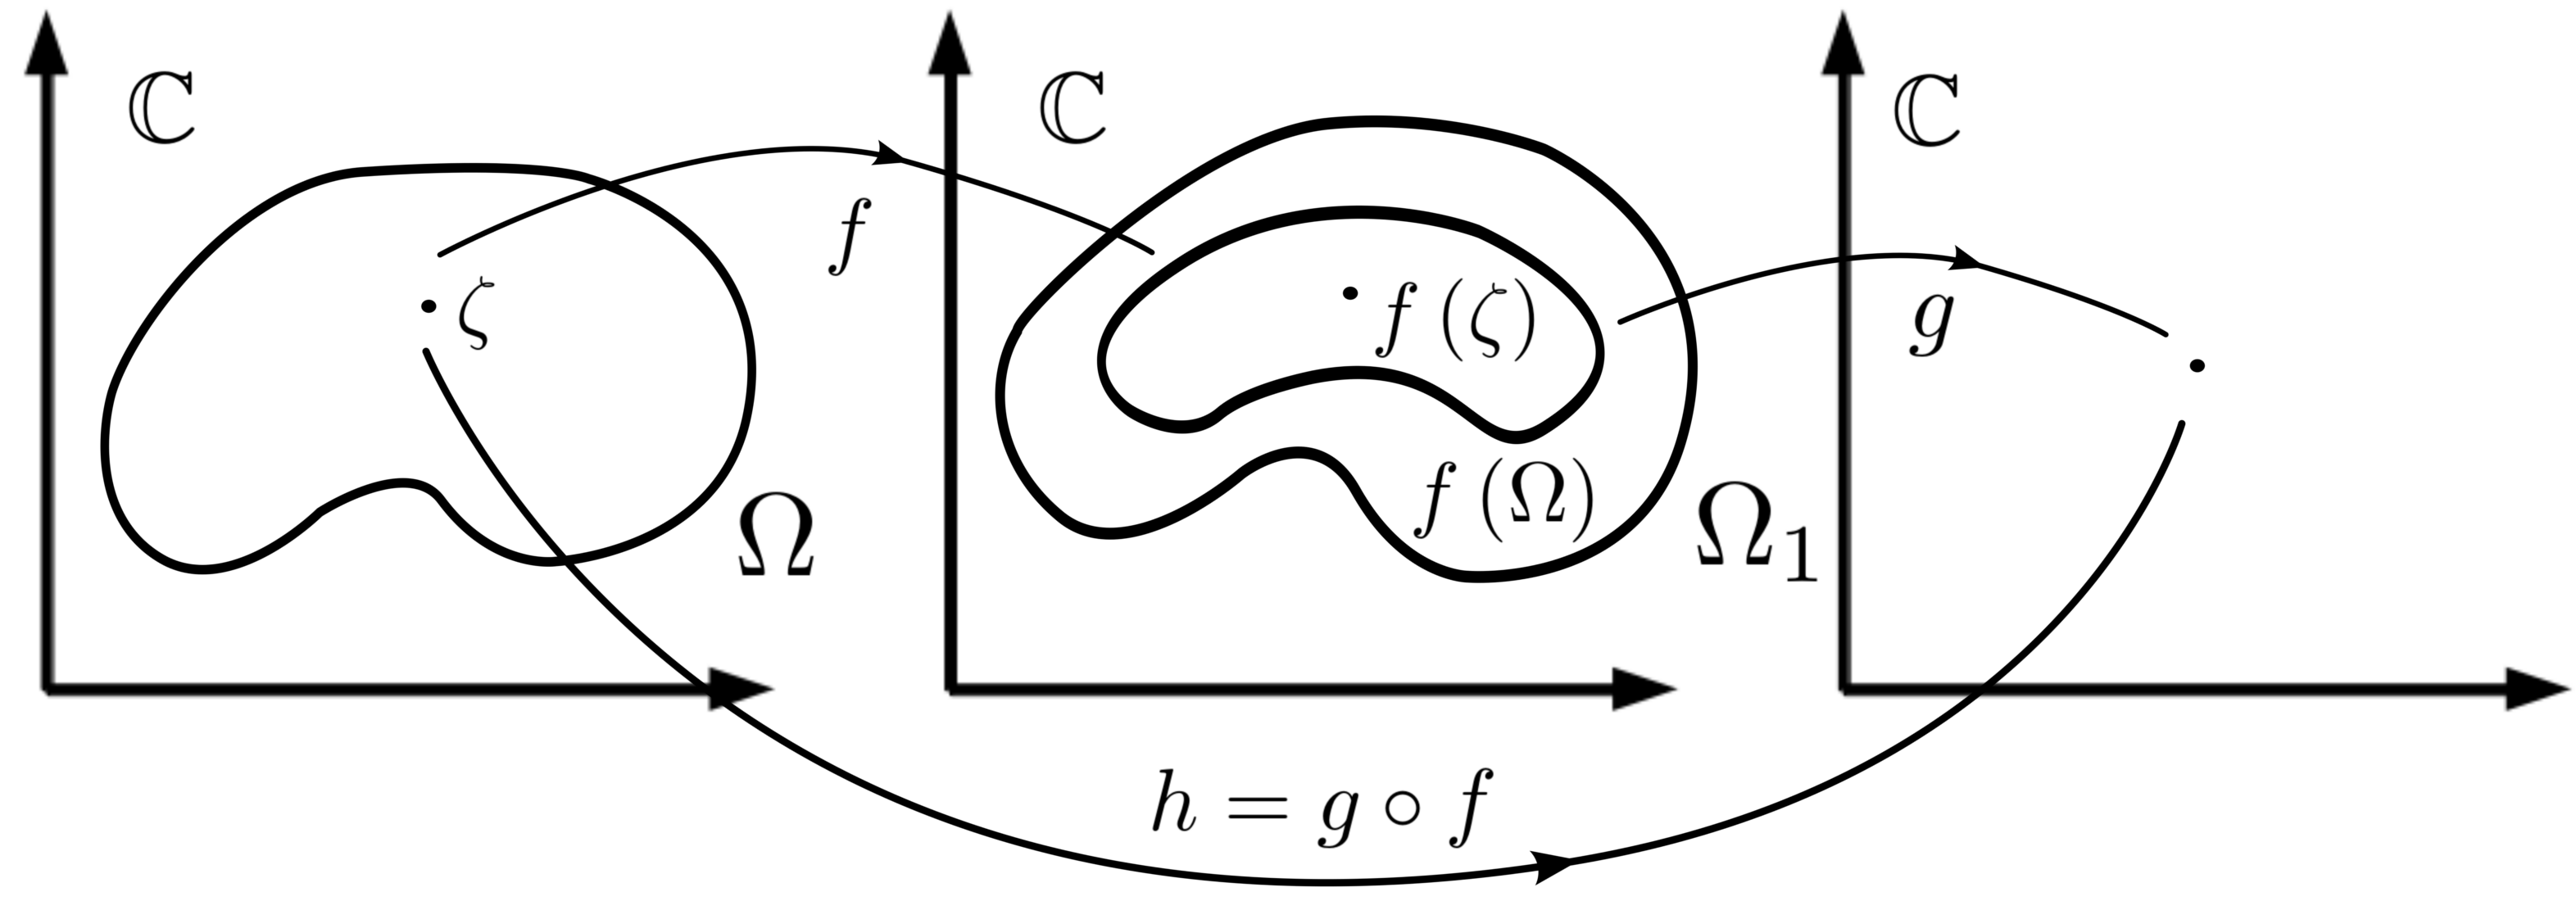
\includegraphics{1.png}
\end{center}

\textit{\bigskip}

\textbf{Prova \ }Dado $\zeta\in\Omega$ temos $\ f(  \zeta)
\in\Omega_{1}$. Como $g$ é diferenciável no ponto

$f(  \zeta)  ,$ existe $r>0$ tal que $D_{r}(  f(
\zeta)  )  \subset\Omega_{1}$ e pelo Lema 1.3, existe

$\psi:D_{r}(  f(  \zeta)  )  \rightarrow%
%TCIMACRO{\U{2102} }%
%BeginExpansion
\mathbb{C}
%EndExpansion
$ tal que

\bigskip

(1.5.1.) \ \ $g\left[  f(  \zeta)  +k\right]  =g\left[  f(
\zeta)  \right]  +k\left\{  g^{\prime}\left[  f(  \zeta)
\right]  +\psi\left[  f(  \zeta)  +k\right]  \right\}  ,$
\ \ $\forall$ \ $k\in D_{r}(  0)  $

\bigskip

onde $\psi$ é contínua em $f(\zeta)$ e $\psi\left[  f(
\zeta)  \right]  =0.$ Pela Prop.1.4 (1%
%TCIMACRO{\U{ba}}%
%BeginExpansion
${{}^o}$%
%EndExpansion
), $f$ é contínua

em $\zeta$ $,$ em consequência existe $\delta>0$ tal que $D_{\delta
}(  \zeta)  \subset\Omega$ e \ $f(  D_{\delta}(
\zeta)  )  \subset$

$D_{r}(  f(  \zeta)  )  ,$ logo dado $h\in D_{\delta
}(  0)  $ arbitrário, temos $\zeta+h\in D_{\delta}(
\zeta)  $ o que

implica $\ f(  \zeta+h)  \in D_{r}(  f(  \zeta)
)  $ e portanto $k:=f(  \zeta+h)  -f(  \zeta)  \in
D_{r}(  0)  ,$ o

que por (1.5.1.) implica (obsevar que $f(  \zeta+h)  =f(
\zeta)  +k$ ) :

\bigskip

(1.5.2.)$\ \ \left\vert
\begin{array}
[c]{c}%
g\left[  f(  \zeta+h)  \right]  =g\left[  f(  \zeta)
\right]  +\left[  f(  \zeta+h)  -f(  \zeta)  \right]
\left\{  g^{\prime}\left[  f(  \zeta)  \right]  +\psi\left[
f(  \zeta)  +k\right]  \right\}  \text{ },\\
\text{para cada\ \ }h\in D_{\delta}(  0)
\text{\ \ \ \ \ \ \ \ \ \ \ \ \ \ \ \ \ \ \ \ \ \ \ \ \ \ \ \ \ \ \ \ \ \ \ \ \ \ \ \ \ \ \ \ \ \ \ \ \ \ \ \ \ \ \ \ \ \ \ \ \ \ }%
\end{array}
\right.  $

\bigskip

Como $\ f$ \ é diferenciável em $\ \zeta,$ pelo Lema 1.3 (i)
$\implies$ (ii), \ existe\footnote{$\delta$ faz aqui o papel do $r$ do Lema 1.3 e a única hipótese sobre $\delta(  r) 
 $ é que $D_{\delta}(  \zeta)  \subset\Omega$ o que é verdade por definição de $\delta$.}

$\varphi:D_{\delta}(  \zeta)  \rightarrow%
%TCIMACRO{\U{2102} }%
%BeginExpansion
\mathbb{C}
%EndExpansion
$ tal que

\bigskip

(1.5.3.) \ \ \ \ \ \ $f(  \zeta+h)  -f(  \zeta)
=h\left[  f^{\prime}(  \zeta)  +\varphi(  \zeta+h)
\right]  $ \ \ \ $\forall$ \ $h\in D_{\delta}(  0)  $

\bigskip onde $\varphi$ é contínua em $\zeta$ e $\varphi(
\zeta)  =0.$ De (1.5.3.) e (1.5.2.) resulta

\bigskip

(1.5.4.) $\ \ \ \ \left\vert
\begin{array}
[c]{c}%
g\left[  f(  \zeta+h)  \right]  =g\left[  f(  \zeta)
\right]  +h\left\{  g^{\prime}\left[  f(  \zeta)  \right]  \cdot
f^{\prime}(  \zeta)  +\eta(  \zeta+h)  \right\}  ,\text{
\ }\\
\forall\ h\in D_{\delta}(  0)
\text{\ \ \ \ \ \ \ \ \ \ \ \ \ \ \ \ \ \ \ \ \ \ \ \ \ \ \ \ \ \ \ \ \ \ \ \ \ \ \ \ \ \ \ \ \ \ \ \ \ \ \ \ \ \ \ \ \ \ \ \ \ }%
\end{array}
\right.  \ \ \ \ $\ 

$\ \ \ \ \ \ \ \ \ \ \ \ \ \ \ \ \ \ \ \ $

onde para cada $h\in D_{\delta}(  0)  $ definimos

$\eta(  \zeta+h)  :=f^{\prime}(  \zeta)  \psi\left[
f(  \zeta+h)  \right]  +g^{\prime}\left[  f(  \zeta)
\right]  \varphi(  \zeta+h)  +\varphi(  \zeta+h)
\psi\lbrack f(  \zeta+h)  ].$ \ 

É imediato verificar que a função $\eta:D_{\delta}(
\zeta)  \rightarrow%
%TCIMACRO{\U{2102} }%
%BeginExpansion
\mathbb{C}
%EndExpansion
,$ que acabamos de definir,

é contínua em $\zeta$ e que $\eta(  \zeta)  =0,$ portanto
(1.5.4) e o Lema 1.3 (ii) $\implies$(i)

demonstram o resultado. \ $\square$


\bigskip

Até agora nossa definição de função holomorfa como
função complexa

definida num aberto de $%
%TCIMACRO{\U{2102} }%
%BeginExpansion
\mathbb{C}
%EndExpansion
$ que é diferenciável em cada ponto do seu

domínio nos permitiu apenas provar alguns resultados básicos que são

formalmente idênticos a resultados conhecidos para funções reais de

variável real. Como aplicação destas propriedades vamos exibir alguns

exemplos simples de funções holomorfas e de funções não holomorfas.

\bigskip

\textbf{Exemplo 1 \ }Para cada $\ m\in%
%TCIMACRO{\U{2115} }%
%BeginExpansion
\mathbb{N}
%EndExpansion
^{\ast}$ seja $\pi_{m}:z\in%
%TCIMACRO{\U{2102} }%
%BeginExpansion
\mathbb{C}
%EndExpansion
\longmapsto z^{m}\in%
%TCIMACRO{\U{2102} }%
%BeginExpansion
\mathbb{C}
%EndExpansion
$ então $\pi_{m}$ é

holomorfa em $%
%TCIMACRO{\U{2102} }%
%BeginExpansion
\mathbb{C}
%EndExpansion
,$ pois é imediato verificar (como no caso real) que se

$\zeta\in%
%TCIMACRO{\U{2102} }%
%BeginExpansion
\mathbb{C}
%EndExpansion
$ é um ponto arbitário, então

\ \ \ \ \ \ \ \ \ \ \ \ \ \ \ $\pi_{m}^{\prime}(  \zeta)
=\underset{z\rightarrow\zeta}{\lim}\frac{%
\begin{array}
[c]{c}%
\\
z^{m}-\zeta^{m}%
\end{array}
}{%
\begin{array}
[c]{c}%
z-\zeta\\
\end{array}
}=m\zeta^{m-1},$ \ \ se $m\in%
%TCIMACRO{\U{2115} }%
%BeginExpansion
\mathbb{N}
%EndExpansion
^{\ast}$

Resulta do que precede e da Prop. 1.4. (2$^{\underline{o}}$) que se $p:%
%TCIMACRO{\U{2102} }%
%BeginExpansion
\mathbb{C}
%EndExpansion
\rightarrow%
%TCIMACRO{\U{2102} }%
%BeginExpansion
\mathbb{C}
%EndExpansion
$ \ é uma

função polinomial com coeficientes complexos

\bigskip
\ \ \ \ \ \ \ \ \ \ \ \ \ \ \ \ \ \ \ \ \ \ \ \ \ \ \ \ \ \ \ \ \ $p=\underset
{k=0}{\overset{m}{\sum}}a_{k}\pi_{k}$\\

onde $m\in%
%TCIMACRO{\U{2115} }%
%BeginExpansion
\mathbb{N}
%EndExpansion
;$ $a_{0},a_{1},$ \ldots\ $a_{m}\in%
%TCIMACRO{\U{2102} }%
%BeginExpansion
\mathbb{C}
%EndExpansion
$ e $\pi_{0}:z\in\mathbb{C} \longmapsto 1 \! \in\mathbb{C}$ 

(isto é, $p(  z)  =\overset{m}{\underset{k=0}{\sum}}%
a_{k}z^{k}$para cada $z\in%
%TCIMACRO{\U{2102} }%
%BeginExpansion
\mathbb{C}
%EndExpansion
$), então $p\in\mathcal{H}(
%TCIMACRO{\U{2102} }%
%BeginExpansion
\mathbb{C}
%EndExpansion
)  .$

\bigskip

\textbf{Exemplo 2} \ A função

\ \ \ \ \ \ \ \ \ \ \ \ \ \ \ \ \ \ \ \ \ \ \ \ \ \ \ \ \ \ \ \ \ \ $g_{0}%
:z\in%
%TCIMACRO{\U{2102} }%
%BeginExpansion
\mathbb{C}
%EndExpansion
^{\ast}\longmapsto\frac{%
\begin{array}
[c]{c}%
\\
1
\end{array}
}{%
\begin{array}
[c]{c}%
z\\
\end{array}
}\in%
%TCIMACRO{\U{2102} }%
%BeginExpansion
\mathbb{C}
%EndExpansion
$

é holomorfa no aberto $%
%TCIMACRO{\U{2102} }%
%BeginExpansion
\mathbb{C}
%EndExpansion
^{\ast}.$ De modo mais geral, fixado $\zeta\in%
%TCIMACRO{\U{2102} }%
%BeginExpansion
\mathbb{C}
%EndExpansion
$

arbitrário, a função

\ \ \ \ \ \ \ \ \ \ \ \ \ \ \ \ \ \ \ \ \ \ \ \ \ \ \ \ \ \ \ \ $g_{\zeta
}:z\in%
%TCIMACRO{\U{2102} }%
%BeginExpansion
\mathbb{C}
%EndExpansion
\diagdown\left\{  \zeta\right\}  \longmapsto\frac{%
\begin{array}
[c]{c}%
\\
1
\end{array}
}{%
\begin{array}
[c]{c}%
z-\zeta\\
\end{array}
}\in%
%TCIMACRO{\U{2102} }%
%BeginExpansion
\mathbb{C}
%EndExpansion
$

é holomorfa no aberto $%
%TCIMACRO{\U{2102} }%
%BeginExpansion
\mathbb{C}
%EndExpansion
\diagdown\left\{  \zeta\right\}  .$ De fato, se $z\in%
%TCIMACRO{\U{2102} }%
%BeginExpansion
\mathbb{C}
%EndExpansion
\diagdown\left\{  \zeta\right\}  $ \ temos

$g_{\zeta}^{\prime}(  z)  =\underset{h\rightarrow0}{\lim}\frac{%
\begin{array}
[c]{c}%
\\
g_{\zeta}(  z+h)  -g_{\zeta}(  z)
\end{array}
}{%
\begin{array}
[c]{c}%
h\\
\end{array}
}=-\underset{h\rightarrow0}{\lim}\frac{%
\begin{array}
[c]{c}%
\\
1
\end{array}
}{%
\begin{array}
[c]{c}%
(  z+h-\zeta)  (  z-\zeta) \\
\end{array}
}=-\frac{%
\begin{array}
[c]{c}%
\\
1
\end{array}
}{%
\begin{array}
[c]{c}%
(  z-\zeta)  ^{2}\\
\end{array}
}.$

\bigskip

\textbf{Exemplo 3} \ Sejam $\Omega$ um aberto não vazio de $%
%TCIMACRO{\U{2102} }%
%BeginExpansion
\mathbb{C}
%EndExpansion
,$ $f_{1}\in\mathcal{H}(  \Omega)  ,$ $f_{2}\in\mathcal{H}(
\Omega)  $

e $\Omega_{0}$ um subconjunto aberto de $\Omega$ no qual $f_{2}\neq0$ (isto
é, $f_{2}(  z)  \neq0$ para

cada $z\in\Omega_{0}$)$.$ Então $f_{1}/f_{2}\in\mathcal{H}(
\Omega_{0})  ,$ onde $(  f_{1}/f_{2})  (  z)
:=f_{1}(  z)  /f_{2}(  z)  $ \ para \ 

cada $z\in\Omega_{0}.$ De fato, basta aplicar a regra da cadeia (Prop. 1.5) subs-

tituindo as funções $g$ e $f$ daquele resultado pelas funções
$g_{0}$ do Exem-

plo 2 e $\ f_{2}$ respectivamente. Então, para cada $z\in\Omega_{0}$
\ temos $f_{2}(  z)  \neq0,$

donde $f_{2}(  \Omega_{0})  \subset%
%TCIMACRO{\U{2102} }%
%BeginExpansion
\mathbb{C}
%EndExpansion
^{\ast}=$ domínio de $g_{0}$ \ e

\ \ \ \ \ \ \ \ \ \ \ \ \ \ \ \ \ $(
%TCIMACRO{\QDOVERD{.}{.}{1}{f_{2}}}%
%BeginExpansion
\genfrac{.}{.}{}{0}{1}{f_{2}}%
%EndExpansion
)  (  z)  =%
%TCIMACRO{\QDOVERD{.}{.}{1}{f_{2}(  z)  }}%
%BeginExpansion
\genfrac{.}{.}{}{0}{1}{f_{2}(  z)  }%
%EndExpansion
=(  g_{0}\circ f_{2})  (  z)  $ \ , \ 

para cada $z\in\Omega_{0}.$ Pela Prop. 1.5 temos então, para $\zeta
\in\Omega_{0}$ arbitrário

fixado:

$(
%TCIMACRO{\QDOVERD{.}{.}{1}{f_{2}}}%
%BeginExpansion
\genfrac{.}{.}{}{0}{1}{f_{2}}%
%EndExpansion
)  ^{\prime}(  \zeta)  =(  g_{0}\circ f_{2})
^{\prime}(  \zeta)  =g_{0}^{\prime}\left[  f_{2}(
\zeta)  \right]  \cdot f_{2}^{\prime}(  \zeta)  =\frac{%
\begin{array}
[c]{c}%
\\
f_{2}^{\prime}(  \zeta)
\end{array}
}{%
\begin{array}
[c]{c}%
\left[  f_{2}(  \zeta)  \right]  ^{2}\\
\end{array}
}$

o que mostra que $1/f_{2}\in\mathcal{H}(  \Omega_{0})  .$ Em
consequência, pela Prop. 1.4 (2$^{\underline{o}}$)

obtemos:

\ \ \ \ \ \ \ \ \ \ \ \ \ \ \ \ \ \ \ \ \ $f_{1}/f_{2}=f_{1}\cdot(
1/f_{2})  $\bigskip$\in\mathcal{H}(  \Omega_{0})  $

Observar que $\ \left[  f_{1}(  1/f_{2})  \right]  ^{\prime}(
\zeta)  =f_{1}^{\prime}(  \zeta)  \frac{%
\begin{array}
[c]{c}%
\\
1
\end{array}
}{%
\begin{array}
[c]{c}%
f_{2}(  \zeta) \\
\end{array}
}+f_{1}(  \zeta)  \left\{  -%
%TCIMACRO{\QDOVERD{.}{.}{f_{2}^{\prime}(  \zeta)  }{\left[
%f_{2}(  \zeta)  \right]  ^{2}}}%
%BeginExpansion
\genfrac{.}{.}{}{0}{f_{2}^{\prime}(  \zeta)  }{\left[  f_{2}(
\zeta)  \right]  ^{2}}%
%EndExpansion
\right\}  =$

$=\frac{%
\begin{array}
[c]{c}%
\\
f_{1}^{\prime}(  \zeta)  f_{2}(  \zeta)  -f_{1}(
\zeta)  f_{2}^{\prime}(  \zeta)
\end{array}
}{%
\begin{array}
[c]{c}%
\left[  f_{2}(  \zeta)  \right]  ^{2}\\
\end{array}
},$ isto é obtemos a regra formal usual de

derivação de um quociente: $(  f_{1}/f_{2})  ^{\prime
}=\frac{%
\begin{array}
[c]{c}%
\\
f_{1}^{\prime}f_{2}-f_{1}f_{2}^{\prime}%
\end{array}
}{%
\begin{array}
[c]{c}%
f_{2}^{2}\\
\end{array}
}$ $.$

\bigskip

\textbf{Exemplo 4} \ Sejam $p$ e $q$ duas funções polinomiais a coeficientes

complexos

\ \ \ \ \ \ \ \ \ \ \ \ \ \ \ \ \ $p(  z)  =\underset{j=0}%
{\overset{m}{\sum}}a_{j}z^{j}$\ \ \ \ \ \ \ \ e \ \ \ \ \ \ \ $q(
z)  =\overset{n}{\underset{k=0}{\sum}}b_{k}z^{k}$ \ \ \ $,$
\ \ \ \ $q\neq0$

Como $q$ tem $n$ raízes complexas contadas com sua multiplicidade, re-

sulta que o conjunto $F$ das raízes de $q$ tem, no máximo, $n$ elementos,

isto é, é finito e portanto fechado, donde resulta que $\ \Omega_{0}=%
%TCIMACRO{\U{2102} }%
%BeginExpansion
\mathbb{C}
%EndExpansion
\diagdown F$ \ é

aberto.

Então a função racional $R$ definida por

\ \ \ \ \ \ \ \ \ \ \ \ \ \ \ \ $R(  z)  =\frac{%
\begin{array}
[c]{c}%
\\
p(  z)
\end{array}
}{%
\begin{array}
[c]{c}%
q(  z) \\
\end{array}
}$ \ \ \ para dada $z\in\Omega_{0}=%
%TCIMACRO{\U{2102} }%
%BeginExpansion
\mathbb{C}
%EndExpansion
\diagdown F$

é holomorfa em $\Omega_{0.\text{ }}$ De fato, esta asserção é
um caso particular do

Exemplo 3 precedente com $\Omega=%
%TCIMACRO{\U{2102} }%
%BeginExpansion
\mathbb{C}
%EndExpansion
,$ \ $f_{1}=p$ \ e \ $f_{2}=q.$\bigskip

\bigskip

\textbf{Exemplo 5} \ A função \ conjugação $J:z\in%
%TCIMACRO{\U{2102} }%
%BeginExpansion
\mathbb{C}
%EndExpansion
\longmapsto\overline{z}\in%
%TCIMACRO{\U{2102} }%
%BeginExpansion
\mathbb{C}
%EndExpansion
$ \ que é um iso-

morfismo involutivo de $%
%TCIMACRO{\U{2102} }%
%BeginExpansion
\mathbb{C}
%EndExpansion
$ sobre $%
%TCIMACRO{\U{2102} }%
%BeginExpansion
\mathbb{C}
%EndExpansion
,$ é uma aplicação contínua e aberta,

não é diferenciável em nenhum ponto de $%
%TCIMACRO{\U{2102} }%
%BeginExpansion
\mathbb{C}
%EndExpansion
$ e portanto $J\notin\mathcal{H}(
%TCIMACRO{\U{2102} }%
%BeginExpansion
\mathbb{C}
%EndExpansion
)  $ e, de

modo mais geral, qualquer que seja o aberto não vazio $\Omega$ de $%
%TCIMACRO{\U{2102} }%
%BeginExpansion
\mathbb{C}
%EndExpansion
$ temos

\ \ \ \ \ \ \ \ \ \ \ \ \ \ \ \ \ \ \ \ \ \ \ \ \ \ \ \ \ \ \ \ \ \ \ \ \ \ $J$
$|$ $\Omega\notin\mathcal{H}(  \Omega)  .$

Com efeito, seja $\zeta\in%
%TCIMACRO{\U{2102} }%
%BeginExpansion
\mathbb{C}
%EndExpansion
$ um ponto arbitrário e mostremos que não existe

o limite

\ \ \ \ \ \ \ \ \ \ \ \ \ \ \ \ \ \ \ \ \ \ \ \ \ \ \ \ \ \ \ \ $\underset
{h\rightarrow0}{\lim}\frac{%
\begin{array}
[c]{c}%
\\
J(  \zeta+h)  -J(  \zeta)
\end{array}
}{%
\begin{array}
[c]{c}%
h\\
\end{array}
}.$

Como $\frac{%
\begin{array}
[c]{c}%
\\
J(  \zeta+h)  -J(  \zeta)
\end{array}
}{%
\begin{array}
[c]{c}%
h\\
\end{array}
}=\frac{%
\begin{array}
[c]{c}%
\\
\overline{h}%
\end{array}
}{%
\begin{array}
[c]{c}%
h\\
\end{array}
},$ basta ver que não existe $\underset{h\rightarrow0}{\lim}\frac{%
\begin{array}
[c]{c}%
\\
\overline{h}%
\end{array}
}{%
\begin{array}
[c]{c}%
h\\
\end{array}
}$ \ o que

é imediato pois se $h\in%
%TCIMACRO{\U{211d} }%
%BeginExpansion
\mathbb{R}
%EndExpansion
^{\ast}$ então $\overline{h}/h=1$ e se $h\in%
%TCIMACRO{\U{211d} }%
%BeginExpansion
\mathbb{R}
%EndExpansion
^{\ast}i=\left\{  ai\text{ }|\text{ }a\in%
%TCIMACRO{\U{211d} }%
%BeginExpansion
\mathbb{R}
%EndExpansion
^{\ast}\right\}  $

então $\overline{h}/h=-1,$ o que mostra que não existe $\underset
{h\rightarrow0}{\lim}\overline{h}/h$ .

\bigskip

\textbf{Exemplo 6} \ A função "módulo"

\ \ \ \ \ \ \ \ \ \ \ \ \ \ \ \ \ \ \ \ \ \ \ \ \ \ \ \ \ \ \ \ \ \ \ \ $f=\left\vert
\cdot\right\vert :z\in%
%TCIMACRO{\U{2102} }%
%BeginExpansion
\mathbb{C}
%EndExpansion
\mapsto\left\vert z\right\vert \in%
%TCIMACRO{\U{211d} }%
%BeginExpansion
\mathbb{R}
%EndExpansion
$

não é derivável em nenhum ponto de $%
%TCIMACRO{\U{2102} }%
%BeginExpansion
\mathbb{C}
%EndExpansion
$ e portanto

\ \ \ \ \ \ \ \ \ \ \ \ \ \ \ \ \ \ \ \ \ \ \ \ \ \ \ \ \ \ \ \ \ \ \ $f\notin
\mathcal{H}(
%TCIMACRO{\U{2102} }%
%BeginExpansion
\mathbb{C}
%EndExpansion
)  .$

De fato, se $\zeta\in%
%TCIMACRO{\U{2102} }%
%BeginExpansion
\mathbb{C}
%EndExpansion
,\zeta\neq0$ então $f=\left\vert \cdot\right\vert $ não é
derivável em $\zeta$ pois se o fosse

então $f^{2\text{ }}$\bigskip\ também seria derivável em $\zeta$ e
como $f^{2}(  z)  =\left\vert z\right\vert ^{2}=z\cdot\overline{z}$ \ para

cada $z\in%
%TCIMACRO{\U{2102} }%
%BeginExpansion
\mathbb{C}
%EndExpansion
,$ isto é,

\ \ \ \ \ \ \ \ \ \ \ \ \ \ \ \ \ \ \ \ \ \ \ \ \ \ \ \ \ \ \ \ \ \ \ \ $f^{2}%
$\bigskip$=id\cdot J$

(onde $id:z\in%
%TCIMACRO{\U{2102} }%
%BeginExpansion
\mathbb{C}
%EndExpansion
\mapsto z\in%
%TCIMACRO{\U{2102} }%
%BeginExpansion
\mathbb{C}
%EndExpansion
$ e\ $J:z\in%
%TCIMACRO{\U{2102} }%
%BeginExpansion
\mathbb{C}
%EndExpansion
\mapsto\overline{z}\in%
%TCIMACRO{\U{2102} }%
%BeginExpansion
\mathbb{C}
%EndExpansion
$)\ resultaria (ver Exemplo 3)

que

\ \ \ \ \ \ \ \ \ \ \ \ \ \ \ \ \ \ \ \ \ \ \ \ \ \ \ \ \ \ \ \ \ \ \ $J=\frac
{%
\begin{array}
[c]{c}%
\\
f^{2}%
\end{array}
}{%
\begin{array}
[c]{c}%
id\\
\end{array}
}$

é derivável em $\zeta$ (pois como $\zeta\neq0$ temos $id(
\zeta)  =\zeta\neq0$) o que é absurdo

como vimos no Exemplo 5. A função $f=\left\vert \cdot\right\vert $
não é derivável em $\zeta=0$ pois

o mesmo tipo de raciocínio do Exemplo 5 mostra que não existe limite

da expressão

\ \ \ \ \ \ \ \ \ \ \ \ \ \ \ \ \ \ \ \ \ \ \ \ \ \ \ \ \ \ \ $\frac{%
\begin{array}
[c]{c}%
\\
f(  h)  -f(  0)
\end{array}
}{%
\begin{array}
[c]{c}%
h\\
\end{array}
}=\frac{%
\begin{array}
[c]{c}%
\\
\left\vert h\right\vert
\end{array}
}{%
\begin{array}
[c]{c}%
h\\
\end{array}
}$

para $h\rightarrow0.$

\bigskip

\textbf{Observação \ }Mais adiante será demonstrado\ de forma
bastante simples

que uma função $f:%
%TCIMACRO{\U{2102} }%
%BeginExpansion
\mathbb{C}
%EndExpansion
\rightarrow%
%TCIMACRO{\U{2102} }%
%BeginExpansion
\mathbb{C}
%EndExpansion
$ verificando as condições:\ \ \ \ \ \ 

$\left[  \ast\right]  $\ \ \ \ \ \ \ \ \ \ \ \ \ \ \ \ \ \ \ \ $\left\{
\begin{array}
[c]{c}%
\text{ \ }f\text{ é
contínua\ \ \ \ \ \ \ \ \ \ \ \ \ \ \ \ \ \ \ \ \ \ \ \ \ \ \ \ \ \ }\\
\text{ }f\text{ não é constante
\ \ \ \ \ \ \ \ \ \ \ \ \ \ \ \ \ \ \ \ \ }\\
\text{\textsc{I}m}(  f)  \subset%
%TCIMACRO{\U{211d} }%
%BeginExpansion
\mathbb{R}
%EndExpansion
\text{\ \ \ \ \ \ \ \ \ \ \ \ \ \ \ \ \ \ \ \ \ \ \ \ \ \ \ \ \ \ }%
\end{array}
\right.  $

não é derivável em nenhum ponto de $%
%TCIMACRO{\U{2102} }%
%BeginExpansion
\mathbb{C}
%EndExpansion
$ e em consequência, qualquer que

seja $\Omega$ temos $f$ $|$ $\Omega\notin\mathcal{H}(  \Omega)  .$
Alguns exemplos simples de funções verificando

as condições $\left[  \ast\right]  $\ \ são os seguintes:

$f(  z)  =\left\vert z\right\vert $\ \ , \ $f(  z)
=\operatorname{Re}(  z)  $\ \ , \ \ $f(  z)
=$\textsc{I}m$(  z)  $\ \ \ , \ \ $f(  z)
=e^{\operatorname{Re}(  z)  }$\ , \ etc. \ De

modo mais geral, se $\Phi:%
%TCIMACRO{\U{211d} }%
%BeginExpansion
\mathbb{R}
%EndExpansion
^{2}$\ $\rightarrow%
%TCIMACRO{\U{211d} }%
%BeginExpansion
\mathbb{R}
%EndExpansion
$ é uma função contínua não constante, então

a função $f:%
%TCIMACRO{\U{2102} }%
%BeginExpansion
\mathbb{C}
%EndExpansion
\rightarrow%
%TCIMACRO{\U{2102} }%
%BeginExpansion
\mathbb{C}
%EndExpansion
$ definida por


\ \ \ \ \ \ \ \ \ \ \ \ \ \ \ \ \ \ \ \ \ \ \ $f(
z)  $\ = $\Phi(  \operatorname{Re}(  z)
,\text{\textsc{I}m}(  z)  )  $\ \ \ para cada $z\in%
%TCIMACRO{\U{2102} }%
%BeginExpansion
\mathbb{C}
%EndExpansion
$


satisfaz as condições $\left[  \ast\right]  $\ e portanto não
é derivável em nenhum ponto de $%
%TCIMACRO{\U{2102} }%
%BeginExpansion
\mathbb{C}
%EndExpansion
$.

Aqui é pertinente o seguinte comentário: Não é trivial
construir uma função

$f:%
%TCIMACRO{\U{211d} }%
%BeginExpansion
\mathbb{R}
%EndExpansion
\rightarrow%
%TCIMACRO{\U{211d} }%
%BeginExpansion
\mathbb{R}
%EndExpansion
$\ que seja contínua em $%
%TCIMACRO{\U{211d} }%
%BeginExpansion
\mathbb{R}
%EndExpansion
$\ e que não seja derivável em nenhum\ pon-

to de $%
%TCIMACRO{\U{211d} }%
%BeginExpansion
\mathbb{R}
%EndExpansion
$, ver por exemplo, \cite{R1}, Cap. 7, Teor. 7.18, ao passo que o Exemplo

5 e o\ Exemplo 6, assim como as considerações acima mostram que é bas-

tante fácil obter\ funções contínuas $f:%
%TCIMACRO{\U{2102} }%
%BeginExpansion
\mathbb{C}
%EndExpansion
\rightarrow%
%TCIMACRO{\U{2102} }%
%BeginExpansion
\mathbb{C}
%EndExpansion
$\ \ que não são deriváveis em ne-

nhum ponto de $%
%TCIMACRO{\U{2102} }%
%BeginExpansion
\mathbb{C}
%EndExpansion
.$\ Este tipo de fenômeno confirma o fato assinalado na

(Obs.1) que segue à Def.1.2\textbf{\ , }a saber \ que a hipótese de
diferenciabilidade\ é 

uma exigência muito mais forte no caso das funções complexas de
variável

complexa que no caso das funções reais de variável real.

\bigskip

\ \ \ \ \ \ \ \ \ \ \ \ \ \ \ \ \ \ \ \ \ \ \ \ \ \ \ \ \ \ \ \ \ \ \ \ \ \ 

\bigskip

\ \ \ \ \ \ \ \ \ \ \ \ \ \ \ \ \ \ \ \ \ \ \ \ \ \ \ \ \ \ \ \ \ \ \ \ \ \ \ \ \ \ \ \ \ \ \textbf{Exercícios}%


\bigskip

\bigskip

\textbf{(1.1)}\ \ (caráter local da holomorfia) \ Dada uma função
$f:\Omega\rightarrow%
%TCIMACRO{\U{2102} }%
%BeginExpansion
\mathbb{C}
%EndExpansion
$ provar

as duas asserções seguintes:

(a) \ Se $(  \Omega_{\lambda})  _{\lambda\in\Lambda}$ é uma
família de abertos não vazios cuja reunião é $\Omega$ \ e

$f$ $|$ $\Omega_{\lambda}\in\mathcal{H}(  \Omega_{\lambda})  $ para
cada $\lambda\in\Lambda,$ então $f\in\mathcal{H}(  \Omega)  ;$

(b) \ Se $\Omega_{0}$ é uma parte aberta não vazia de $\Omega,$
então $f$ $|$ $\Omega_{0}\in\mathcal{H}(  \Omega_{0})  $ desde

que $f\in\mathcal{H}(  \Omega)  .$

\bigskip

\textbf{(1.2) \ }Seja $A=(  \left[  0,1\right]  \times\left[
0,1\right]  )  \cap(
%TCIMACRO{\U{211a} }%
%BeginExpansion
\mathbb{Q}
%EndExpansion
\times%
%TCIMACRO{\U{211a} }%
%BeginExpansion
\mathbb{Q}
%EndExpansion
)  \subset%
%TCIMACRO{\U{2102} }%
%BeginExpansion
\mathbb{C}
%EndExpansion
$ \ e \ $f:A\rightarrow%
%TCIMACRO{\U{2102} }%
%BeginExpansion
\mathbb{C}
%EndExpansion
$ \ a função

identidade (i.e. $f(  z)  =z$ \ \ $\forall$ \ \ $z\in A$).
Verificar que \ $\underset{z\rightarrow\zeta}{\lim}%
%TCIMACRO{\QDOVERD{.}{.}{f(  z)  -f(  \zeta)  }{z-\zeta
%}}%
%BeginExpansion
\genfrac{.}{.}{}{0}{f(  z)  -f(  \zeta)  }{z-\zeta}%
%EndExpansion
=1$

para cada $\zeta\in A$ e porém $f$ \ não é derivável em nenhum
ponto de $A.$

\bigskip

\textbf{(1.3)} \ Seja $\Omega$ um aberto não vazio de $%
%TCIMACRO{\U{2102} }%
%BeginExpansion
\mathbb{C}
%EndExpansion
$ tal que $\Omega$ é simétrico em relação

ao eixo real (i.e. $z\in\Omega\implies\overline{z}\in\Omega$). Mostrar que se
$f\in\mathcal{H}(  \Omega)  ,$ então a

função $\ g:\Omega\rightarrow%
%TCIMACRO{\U{2102} }%
%BeginExpansion
\mathbb{C}
%EndExpansion
$ definida por $g(  z)  =\overline{f(  \overline{z})  }%
$, para cada $z\in\Omega$ é holomorfa.

\bigskip

\textbf{(1.4) } (sobre a topologia do plano) \ Dado um subconjunto $X$ de $%
%TCIMACRO{\U{2102} }%
%BeginExpansion
\mathbb{C}
%EndExpansion
$ chama-

se \textit{fronteira }de $X$ o conjunto:

\ \ \ \ \ \ \ \ \ \ \ \ \ \ \ \ \ \ \ \ \ \ \ \ \ \ \ \ \ \ \ \ $\partial
X=\overline{X}\cap(  \overline{%
%TCIMACRO{\U{2102} }%
%BeginExpansion
\mathbb{C}
%EndExpansion
\backslash X})  $

(a) \ Prove que $\xi\in\partial X$ se e só se $D_{\varepsilon}(
\xi)  \cap X\neq\varnothing$ \ e \ $D_{\varepsilon}(  \xi)
\cap(
%TCIMACRO{\U{2102} }%
%BeginExpansion
\mathbb{C}
%EndExpansion
\backslash X)  \neq\varnothing$

para cada $\varepsilon>0;$

(b) \ Mostre que $\partial X=\partial(
%TCIMACRO{\U{2102} }%
%BeginExpansion
\mathbb{C}
%EndExpansion
\backslash X)  ;$

(c) \ Verifique que para cada $X\subset%
%TCIMACRO{\U{2102} }%
%BeginExpansion
\mathbb{C}
%EndExpansion
,$ $\partial X$ \ é um conjunto fechado;

(d) \ Prove que se $X$ é limitado então $\partial X$ é compacto e
mostre com um

exemplo que a recíproca desta asserção é falsa;

(e) Verifique que se $\xi\in%
%TCIMACRO{\U{2102} }%
%BeginExpansion
\mathbb{C}
%EndExpansion
$ e $r>0$ então

$\ \ \ \ \ \ \ \ \ \ \ \ \ \ \ \ \ \ \partial D_{r}(  \xi)
=\partial\overline{D}_{r}(  \xi)  =\{z\in%
%TCIMACRO{\U{2102} }%
%BeginExpansion
\mathbb{C}
%EndExpansion
$ $|$ $\left\vert z-\xi\right\vert =r\};$

(f) \ Prove que se $\partial\varnothing=\varnothing,$ $\partial%
%TCIMACRO{\U{2102} }%
%BeginExpansion
\mathbb{C}
%EndExpansion
=\varnothing$ \ e que $\partial(
%TCIMACRO{\U{211a} }%
%BeginExpansion
\mathbb{Q}
%EndExpansion
\left[  i\right]  )  =%
%TCIMACRO{\U{2102} }%
%BeginExpansion
\mathbb{C}
%EndExpansion
,$ onde

$%
%TCIMACRO{\U{211a} }%
%BeginExpansion
\mathbb{Q}
%EndExpansion
\left[  i\right]  =\left\{  a+bi\text{ }|\text{ }a,b\in%
%TCIMACRO{\U{211a} }%
%BeginExpansion
\mathbb{Q}
%EndExpansion
\right\}  .$

\bigskip

\textbf{(1.5)} \ Sejam $\Omega$ e $\Sigma$ dois abertos não vazios de $%
%TCIMACRO{\U{2102} }%
%BeginExpansion
\mathbb{C}
%EndExpansion
$ tais que

$\partial\Omega\cap\Sigma\neq\varnothing.$

(a) \ Mostre que $W=\Omega\cap\Sigma\neq\varnothing;$

(b) \ Sejam $g\in\mathcal{C}(  \Sigma)  $ e $f:\Omega\rightarrow%
%TCIMACRO{\U{2102} }%
%BeginExpansion
\mathbb{C}
%EndExpansion
$ uma função e suponha que $f$ $|$ $W=g$ $|$ $W,$

mostre que para cada $\zeta\in\partial\Omega\cap\Sigma,$ existe $\underset
{z\rightarrow\zeta}{\lim}f(  z)  $ e \ que $\ \underset
{z\rightarrow\zeta}{\lim}f(  z)  =$

$\underset{z\rightarrow\zeta}{\lim}g(  z)  =g(  \zeta)
;$

(c) \ Ache uma função $h\in\mathcal{H}(  \Omega)  $ tal que
$h$ $|$ $W\neq g$ $|$ $W$ para cada $g\in\mathcal{C}(  \Sigma)  .$

[\textit{Sugestão:} \ Tomar $\zeta\in\partial\Omega\cap\Sigma$ e definir
$h(  z)  =\frac{%
\begin{array}
[c]{c}%
\\
1
\end{array}
}{%
\begin{array}
[c]{c}%
z-\zeta\\
\end{array}
}$ \ $\forall$ \ $z\in\Omega$].

\bigskip

\textbf{(1.6)} \ Sejam $\Omega$ um aberto não vazio de $%
%TCIMACRO{\U{2102} }%
%BeginExpansion
\mathbb{C}
%EndExpansion
$ e $\zeta\in\Omega.$ Prove que o

conjunto $\mathcal{M}_{\zeta}=\left\{  f\in\mathcal{H}(  \Omega)
\text{ }|\text{ }f(  \zeta)  =0\right\}  $ é um ideal maximal
do anel $\mathcal{H}(  \Omega)  $

[\textit{Sugestão: \ }Verifique que a aplicação $f\in
\mathcal{H}(  \Omega)  \longmapsto f(  \zeta)  \in%
%TCIMACRO{\U{2102} }%
%BeginExpansion
\mathbb{C}
%EndExpansion
$ é um

homomorfismo sobrejetor de anéis.]

\bigskip

\textbf{(1.7) \ Seja }$\Omega$ um aberto conexo simétrico em
relação ao eixo

real, tendo intersecção não vazia \textsc{I} com este. Prove que
toda $f\in\mathcal{H}(  \Omega)  $

se escreve de maneira única na forma

\ \ \ \ \ \ \ \ \ \ \ \ \ \ \ \ \ \ \ \ \ \ \ \ \ \ \ \ \ \ \ \ \ \ \ $f=g+ih
$

onde $g,h\in\mathcal{H}(  \Omega)  $ são tais que $g(
z)  $ e $h(  z)  $ são reais para cada $z\in$ \textsc{I.
}

Verifique que se tem

\ \ \ \ \ \ \ \ \ $\overline{g(  \overline{z})  }=g(
z)  $ \ , \ $h(  \overline{z})  =\overline{h(  z)
}$ \ \ e \ \ $\overline{f(  \overline{z})  }=g(  z)
-ih(  z)  $ \ \ $\forall$ \ $z\in\Omega.$

\pagebreak

% Capítulo 2: As equações da Cauchy-Riemann

\textbf{{\fontsize{18}{18}\selectfont Capítulo 2\\\\}}

\textbf{{\fontsize{20}{20}\selectfont \ \  AS EQUAÇÕES DE \\}}

\textbf{{\fontsize{20}{20}\selectfont \ \  CAUCHY-RIEMANN \\\\\\}}

\bigskip

Dada $f:\Omega\rightarrow%
%TCIMACRO{\U{2102} }%
%BeginExpansion
\mathbb{C}
%EndExpansion
$ podemos pensar em $f$ como uma aplicação de $\Omega\subset%
%TCIMACRO{\U{211d} }%
%BeginExpansion
\mathbb{R}
%EndExpansion
^{2}$

em $%
%TCIMACRO{\U{211d} }%
%BeginExpansion
\mathbb{R}
%EndExpansion
^{2}.$ Se escrevemos $f$ em termos de parte real e parte imaginária

$\ \ \ \ \ \ \ \ \ \ \ \ \ f(  z)  =f(  x+iy)  =f(
x,y)  =u(  x,y)  +iv(  x,y)  =(  u(
x,y)  ,v(  x,y)  )  $\bigskip

sendo $u(  x,y)  \in%
%TCIMACRO{\U{211d} }%
%BeginExpansion
\mathbb{R}
%EndExpansion
$ e $v(  x,y)  \in%
%TCIMACRO{\U{211d} }%
%BeginExpansion
\mathbb{R}
%EndExpansion
$ para cada $z=x+iy\in\Omega,$ é razoável

perguntar o que significa a condição de diferenciabilidade sobre $f$ \ em

termos de derivabilidade das funções reais $u$ e $v.$ A fim de tornar clara

a relação que há entre diferenciabilidade de funções de $%
%TCIMACRO{\U{211d} }%
%BeginExpansion
\mathbb{R}
%EndExpansion
^{2}$ em $%
%TCIMACRO{\U{211d} }%
%BeginExpansion
\mathbb{R}
%EndExpansion
^{2}$ (i.e.

$%
%TCIMACRO{\U{211d} }%
%BeginExpansion
\mathbb{R}
%EndExpansion
$-diferenciabilidade) e diferenciabilidade de funções de $%
%TCIMACRO{\U{2102} }%
%BeginExpansion
\mathbb{C}
%EndExpansion
$ em $%
%TCIMACRO{\U{2102} }%
%BeginExpansion
\mathbb{C}
%EndExpansion
$ no sen-

tido da Def. 1.1 (i.e. $%
%TCIMACRO{\U{2102} }%
%BeginExpansion
\mathbb{C}
%EndExpansion
$-diferenciabilidade) vamos começar provando um

resultado muito simples de álgebra linear em dimensão $2.$ O conjunto

$%
%TCIMACRO{\U{2102} }%
%BeginExpansion
\mathbb{C}
%EndExpansion
=%
%TCIMACRO{\U{211d} }%
%BeginExpansion
\mathbb{R}
%EndExpansion
^{2}$ é de modo natural um $%
%TCIMACRO{\U{211d} }%
%BeginExpansion
\mathbb{R}
%EndExpansion
$-espaço vetorial de dimensão $2$, por outro

lado, como $%
%TCIMACRO{\U{2102} }%
%BeginExpansion
\mathbb{C}
%EndExpansion
$ é um corpo resulta que $%
%TCIMACRO{\U{2102} }%
%BeginExpansion
\mathbb{C}
%EndExpansion
$ é um $%
%TCIMACRO{\U{2102} }%
%BeginExpansion
\mathbb{C}
%EndExpansion
$-espaço vetorial de dimensão

$1$. Lembremos que uma aplicação $u:%
%TCIMACRO{\U{2102} }%
%BeginExpansion
\mathbb{C}
%EndExpansion
\rightarrow%
%TCIMACRO{\U{2102} }%
%BeginExpansion
\mathbb{C}
%EndExpansion
$ é $%
%TCIMACRO{\U{211d} }%
%BeginExpansion
\mathbb{R}
%EndExpansion
$-\textit{linear} se satisfaz as duas

condições seguintes:

(A) \ $u$ é aditiva \ (i.e. $u(  z_{1}+z_{2})  =u(
z_{1})  +u(  z_{2})  $ \ \ $\forall$ \ $z_{1},z_{2}\in%
%TCIMACRO{\U{2102} }%
%BeginExpansion
\mathbb{C}
%EndExpansion
$)

\bigskip($%
%TCIMACRO{\U{211d} }%
%BeginExpansion
\mathbb{R}
%EndExpansion
$H) \ $u$ é $%
%TCIMACRO{\U{211d} }%
%BeginExpansion
\mathbb{R}
%EndExpansion
$-homogênea (i.e. \ $u(  az)  =a\cdot u(  z)  $
\ \ $\forall$ $\ a\in%
%TCIMACRO{\U{211d} }%
%BeginExpansion
\mathbb{R}
%EndExpansion
,z\in%
%TCIMACRO{\U{2102} }%
%BeginExpansion
\mathbb{C}
%EndExpansion
$)

\bigskip

Por outro lado $u:%
%TCIMACRO{\U{2102} }%
%BeginExpansion
\mathbb{C}
%EndExpansion
\rightarrow%
%TCIMACRO{\U{2102} }%
%BeginExpansion
\mathbb{C}
%EndExpansion
$ é dita $%
%TCIMACRO{\U{2102} }%
%BeginExpansion
\mathbb{C}
%EndExpansion
$-\textit{linear} se satisfaz as duas condições

seguintes:

(A) \ \ $u$ é aditiva

($%
%TCIMACRO{\U{2102} }%
%BeginExpansion
\mathbb{C}
%EndExpansion
$H) \ $u$ é $%
%TCIMACRO{\U{2102} }%
%BeginExpansion
\mathbb{C}
%EndExpansion
$-homogênea (i.e. \ $u(  \lambda z)  =\lambda\cdot u(
z)  $ \ \ $\forall$ \ $\lambda\in%
%TCIMACRO{\U{2102} }%
%BeginExpansion
\mathbb{C}
%EndExpansion
,z\in%
%TCIMACRO{\U{2102} }%
%BeginExpansion
\mathbb{C}
%EndExpansion
$)

\bigskip

É claro que toda aplicação $u:%
%TCIMACRO{\U{2102} }%
%BeginExpansion
\mathbb{C}
%EndExpansion
\rightarrow%
%TCIMACRO{\U{2102} }%
%BeginExpansion
\mathbb{C}
%EndExpansion
$ que é $%
%TCIMACRO{\U{2102} }%
%BeginExpansion
\mathbb{C}
%EndExpansion
$-linear é também $%
%TCIMACRO{\U{211d} }%
%BeginExpansion
\mathbb{R}
%EndExpansion
$-linear pois

$(
%TCIMACRO{\U{2102} }%
%BeginExpansion
\mathbb{C}
%EndExpansion
\text{H})  \implies(
%TCIMACRO{\U{211d} }%
%BeginExpansion
\mathbb{R}
%EndExpansion
\text{H})  $. O resultado seguinte mostra as relações existentes entre

aplicações $%
%TCIMACRO{\U{211d} }%
%BeginExpansion
\mathbb{R}
%EndExpansion
$-lineares e $%
%TCIMACRO{\U{2102} }%
%BeginExpansion
\mathbb{C}
%EndExpansion
$-lineares de $%
%TCIMACRO{\U{2102} }%
%BeginExpansion
\mathbb{C}
%EndExpansion
$ em $%
%TCIMACRO{\U{2102} }%
%BeginExpansion
\mathbb{C}
%EndExpansion
.$

\bigskip

\textbf{Lema 2.1} \ \textit{Dados }$\alpha,\beta\in%
%TCIMACRO{\U{2102} }%
%BeginExpansion
\mathbb{C}
%EndExpansion
$\textit{\ arbitrários, consideremos a aplicação}

\textit{\ \ \ \ \ \ \ \ \ \ \ \ \ \ \ \ \ \ \ \ \ \ \ \ \ \ \ \ }%
$L_{\alpha,\beta}:(  x,y)  \in%
%TCIMACRO{\U{211d} }%
%BeginExpansion
\mathbb{R}
%EndExpansion
^{2}=%
%TCIMACRO{\U{2102} }%
%BeginExpansion
\mathbb{C}
%EndExpansion
\longmapsto\alpha x+\beta y\in%
%TCIMACRO{\U{2102} }%
%BeginExpansion
\mathbb{C}
%EndExpansion
,$

\textit{então temos as asserções seguintes:}

(1$^{\underline{o}}$) \ \textit{A aplicação }$L_{\alpha,\beta}%
$\textit{\ é }$%
%TCIMACRO{\U{211d} }%
%BeginExpansion
\mathbb{R}
%EndExpansion
$\textit{-linear. Reciprocamente, se }$L:%
%TCIMACRO{\U{2102} }%
%BeginExpansion
\mathbb{C}
%EndExpansion
\rightarrow%
%TCIMACRO{\U{2102} }%
%BeginExpansion
\mathbb{C}
%EndExpansion
$\textit{\ é }$%
%TCIMACRO{\U{211d} }%
%BeginExpansion
\mathbb{R}
%EndExpansion
$\textit{-linear,}

\textit{então existem }$\alpha\in%
%TCIMACRO{\U{2102} }%
%BeginExpansion
\mathbb{C}
%EndExpansion
$\textit{\ e }$\beta\in%
%TCIMACRO{\U{2102} }%
%BeginExpansion
\mathbb{C}
%EndExpansion
$\textit{\ (únicos) tais que }$L=L_{\alpha,\beta}.$

(2$^{\underline{o}}$) \ \textit{As três condições seguintes
são equivalentes:}

\textit{(i) \ }$\ \ L_{\alpha,\beta}\left[  i(  x,y)  \right]
=i\cdot L_{\alpha,\beta}(  x,y)  $\textit{\ \ , \ para cada
}$(  x,y)  \in%
%TCIMACRO{\U{2102} }%
%BeginExpansion
\mathbb{C}
%EndExpansion
=%
%TCIMACRO{\U{211d} }%
%BeginExpansion
\mathbb{R}
%EndExpansion
^{2}.$

\textit{(ii) \ }$\ L_{\alpha,\beta}$\textit{\ é }$%
%TCIMACRO{\U{2102} }%
%BeginExpansion
\mathbb{C}
%EndExpansion
$\textit{-linear.}

\textit{(iii) \ }$\beta=\alpha i.$

\bigskip

\textbf{Prova \ (}1$^{\underline{o}}$) \ É óbvio que $L_{\alpha,\beta
}$ é $%
%TCIMACRO{\U{211d} }%
%BeginExpansion
\mathbb{R}
%EndExpansion
$-linear. Reciprocamente, se $L:%
%TCIMACRO{\U{2102} }%
%BeginExpansion
\mathbb{C}
%EndExpansion
\rightarrow%
%TCIMACRO{\U{2102} }%
%BeginExpansion
\mathbb{C}
%EndExpansion
$

é $%
%TCIMACRO{\U{211d} }%
%BeginExpansion
\mathbb{R}
%EndExpansion
$-linear, então dado

\ \ \ \ \ \ \ \ \ \ \ \ \ \ \ \ \ \ \ \ \ \ \ $(  x,y)
=x+iy=x(  1,0)  +y(  0,1)  \in%
%TCIMACRO{\U{2102} }%
%BeginExpansion
\mathbb{C}
%EndExpansion
$

temos: $L(  x,y)  =xL(  1,0)  +yL(  0,1)
=L_{\alpha,\beta}(  x,y)  ,$ onde $\alpha=L(  1,0)  $ \ e

$\beta=L(  0,1)  .$

(2$^{\underline{o}}$) \ (i)$\implies$(ii): \ Por (a), $L_{\alpha,\beta}$ é
$\
%TCIMACRO{\U{211d} }%
%BeginExpansion
\mathbb{R}
%EndExpansion
$-linear e portanto aditiva, em conse-

quência basta verificar que $L_{\alpha,\beta}$ é $%
%TCIMACRO{\U{2102} }%
%BeginExpansion
\mathbb{C}
%EndExpansion
$-homogênea. Dados $\lambda=(  u,v)  =$

$u+iv\in%
%TCIMACRO{\U{2102} }%
%BeginExpansion
\mathbb{C}
%EndExpansion
$\ \ e $\ \ z=(  x,y)  \in%
%TCIMACRO{\U{2102} }%
%BeginExpansion
\mathbb{C}
%EndExpansion
$ \ \ temos: $\ \ \ L_{\alpha,\beta}(  \lambda z)  =L_{\alpha
,\beta}\left[  (  u+iv)  z\right]  =$

$L_{\alpha,\beta}(  uz+ivz)  =L_{\alpha,\beta}(  uz)
+L_{\alpha,\beta}(  ivz)  =uL_{\alpha,\beta}(  z)
+ivL_{\alpha,\beta}(  z)  =$

$\lambda\cdot L_{\alpha,\beta}(  z)  $

(ii)$\implies$(i): Claro

(i)$\iff$(iii) \ Como $L_{\alpha,\beta}\left[  i(  x,y)  \right]
=L_{\alpha,\beta}(  -y,x)  =-\alpha y+\beta x$ \ e $\ \ iL_{\alpha
,\beta}(  x,y)  =$

$i(  \alpha x+\beta y)  =\alpha ix+\beta iy,$ \ é claro que (i)
equivale a

\ \ \ \ \ \ \ \ \ \ \ \ \ \ \ \ \ \ \ \ $-\alpha y+\beta x=\alpha ix+\beta
iy,$ \ \ $\forall$ \ $(  x,y)  \in%
%TCIMACRO{\U{2102} }%
%BeginExpansion
\mathbb{C}
%EndExpansion
$

ou seja

\ \ \ \ \ \ \ \ \ \ \ \ \ \ \ \ \ \ \ \ $(  \alpha i-\beta)
x+(  \alpha+i\beta)  y=0$ \ \ $\forall$ \ $(  x,y)  \in%
%TCIMACRO{\U{2102} }%
%BeginExpansion
\mathbb{C}
%EndExpansion
=%
%TCIMACRO{\U{211d} }%
%BeginExpansion
\mathbb{R}
%EndExpansion
^{2}$

o que é equivalente a $\alpha i-\beta=0$ e $\alpha+i\beta=0$ ou seja
$\beta=\alpha i$ $.$ $\square$

\bigskip

Se identificamos $%
%TCIMACRO{\U{211d} }%
%BeginExpansion
\mathbb{R}
%EndExpansion
$ com sua imagem em $%
%TCIMACRO{\U{211d} }%
%BeginExpansion
\mathbb{R}
%EndExpansion
^{2}$ pela imersão canônica

$J:x\in%
%TCIMACRO{\U{211d} }%
%BeginExpansion
\mathbb{R}
%EndExpansion
\longmapsto(  x,0)  \in%
%TCIMACRO{\U{211d} }%
%BeginExpansion
\mathbb{R}
%EndExpansion
^{2}$ podemos escrever $%
%TCIMACRO{\U{211d} }%
%BeginExpansion
\mathbb{R}
%EndExpansion
\subset%
%TCIMACRO{\U{211d} }%
%BeginExpansion
\mathbb{R}
%EndExpansion
^{2}$ e então é claro que

\ \ \ \ \ \ \ \ \ \ \ \ \ \ \ \ \ \ \ \ \ \ \ \ \ \ \ $%
%TCIMACRO{\U{211d} }%
%BeginExpansion
\mathbb{R}
%EndExpansion
^{2\ast}=\mathcal{L}_{%
%TCIMACRO{\U{211d} }%
%BeginExpansion
\mathbb{R}
%EndExpansion
}(
%TCIMACRO{\U{211d} }%
%BeginExpansion
\mathbb{R}
%EndExpansion
^{2};%
%TCIMACRO{\U{211d} }%
%BeginExpansion
\mathbb{R}
%EndExpansion
)  \subset\mathcal{L}_{%
%TCIMACRO{\U{211d} }%
%BeginExpansion
\mathbb{R}
%EndExpansion
}(
%TCIMACRO{\U{211d} }%
%BeginExpansion
\mathbb{R}
%EndExpansion
^{2};%
%TCIMACRO{\U{211d} }%
%BeginExpansion
\mathbb{R}
%EndExpansion
^{2})  .$

Por outro lado, como toda $u\in\mathcal{L}_{%
%TCIMACRO{\U{2102} }%
%BeginExpansion
\mathbb{C}
%EndExpansion
}(
%TCIMACRO{\U{2102} }%
%BeginExpansion
\mathbb{C}
%EndExpansion
;%
%TCIMACRO{\U{2102} }%
%BeginExpansion
\mathbb{C}
%EndExpansion
)  $ é em particular $%
%TCIMACRO{\U{211d} }%
%BeginExpansion
\mathbb{R}
%EndExpansion
$-homogênea

resulta

\ \ \ \ \ \ \ \ \ \ \ \ \ \ \ \ \ \ \ \ \ \ \ \ \ $\mathcal{L}_{%
%TCIMACRO{\U{2102} }%
%BeginExpansion
\mathbb{C}
%EndExpansion
}(%
%TCIMACRO{\U{2102} }%
%BeginExpansion
\mathbb{C}
%EndExpansion
;%
%TCIMACRO{\U{2102} }%
%BeginExpansion
\mathbb{C}
%EndExpansion
)\subset\mathcal{L}_{%
%TCIMACRO{\U{211d} }%
%BeginExpansion
\mathbb{R}
%EndExpansion
}(
%TCIMACRO{\U{211d} }%
%BeginExpansion
\mathbb{R}
%EndExpansion
^{2};%
%TCIMACRO{\U{211d} }%
%BeginExpansion
\mathbb{R}
%EndExpansion
^{2})  .$

Se indicamos com $\mathcal{L}_{\overline{%
%TCIMACRO{\U{2102} }%
%BeginExpansion
\mathbb{C}
%EndExpansion
}}(
%TCIMACRO{\U{2102} }%
%BeginExpansion
\mathbb{C}
%EndExpansion
;%
%TCIMACRO{\U{2102} }%
%BeginExpansion
\mathbb{C}
%EndExpansion
)  $ o espaço vetorial real de todas as aplicações

$%
%TCIMACRO{\U{2102} }%
%BeginExpansion
\mathbb{C}
%EndExpansion
$-semilineares de $%
%TCIMACRO{\U{2102} }%
%BeginExpansion
\mathbb{C}
%EndExpansion
$ em $%
%TCIMACRO{\U{2102} }%
%BeginExpansion
\mathbb{C}
%EndExpansion
$ (isto é, $u\in\mathcal{L}_{\overline{%
%TCIMACRO{\U{2102} }%
%BeginExpansion
\mathbb{C}
%EndExpansion
}}(
%TCIMACRO{\U{2102} }%
%BeginExpansion
\mathbb{C}
%EndExpansion
;%
%TCIMACRO{\U{2102} }%
%BeginExpansion
\mathbb{C}
%EndExpansion
)  $ se e só se $u$ é uma apli-

cação $%
%TCIMACRO{\U{211d} }%
%BeginExpansion
\mathbb{R}
%EndExpansion
$-linear de $%
%TCIMACRO{\U{2102} }%
%BeginExpansion
\mathbb{C}
%EndExpansion
$ em $%
%TCIMACRO{\U{2102} }%
%BeginExpansion
\mathbb{C}
%EndExpansion
$ tal que $u(  \lambda z)  =\overline{\lambda}u(  z)  $
\ \ $\forall$ \ $\lambda\in%
%TCIMACRO{\U{2102} }%
%BeginExpansion
\mathbb{C}
%EndExpansion
$ \ \ $\forall$ \ $z\in%
%TCIMACRO{\U{2102} }%
%BeginExpansion
\mathbb{C}
%EndExpansion
$) en-

tão é claro que

\ \ \ \ \ \ \ \ \ \ \ \ \ \ \ \ \ \ \ \ \ \ \ \ \ $\mathcal{L}_{\overline{%
%TCIMACRO{\U{2102} }%
%BeginExpansion
\mathbb{C}
%EndExpansion
}}(
%TCIMACRO{\U{2102} }%
%BeginExpansion
\mathbb{C}
%EndExpansion
;%
%TCIMACRO{\U{2102} }%
%BeginExpansion
\mathbb{C}
%EndExpansion
)  \subset\mathcal{L}_{%
%TCIMACRO{\U{211d} }%
%BeginExpansion
\mathbb{R}
%EndExpansion
}(
%TCIMACRO{\U{211d} }%
%BeginExpansion
\mathbb{R}
%EndExpansion
^{2};%
%TCIMACRO{\U{211d} }%
%BeginExpansion
\mathbb{R}
%EndExpansion
_{2})  .$

O resultado seguinte reune uma série de fatos triviais porém úteis para

a compreensão do que se segue.

\bigskip

\textbf{Lema 2.2} \ (1$^{\underline{o}}$) \ $\mathcal{L}_{%
%TCIMACRO{\U{211d} }%
%BeginExpansion
\mathbb{R}
%EndExpansion
}(
%TCIMACRO{\U{2102} }%
%BeginExpansion
\mathbb{C}
%EndExpansion
;%
%TCIMACRO{\U{2102} }%
%BeginExpansion
\mathbb{C}
%EndExpansion
)  =\mathcal{L}_{%
%TCIMACRO{\U{2102} }%
%BeginExpansion
\mathbb{C}
%EndExpansion
}(
%TCIMACRO{\U{2102} }%
%BeginExpansion
\mathbb{C}
%EndExpansion
;%
%TCIMACRO{\U{2102} }%
%BeginExpansion
\mathbb{C}
%EndExpansion
)  \oplus\mathcal{L}_{\overline{%
%TCIMACRO{\U{2102} }%
%BeginExpansion
\mathbb{C}
%EndExpansion
}}(
%TCIMACRO{\U{2102} }%
%BeginExpansion
\mathbb{C}
%EndExpansion
;%
%TCIMACRO{\U{2102} }%
%BeginExpansion
\mathbb{C}
%EndExpansion
)  $

\bigskip

(2$^{\underline{o}}$) \ \textit{Para cada \ }$A\in\mathcal{L}_{%
%TCIMACRO{\U{211d} }%
%BeginExpansion
\mathbb{R}
%EndExpansion
}(
%TCIMACRO{\U{211d} }%
%BeginExpansion
\mathbb{R}
%EndExpansion
^{2},\mathbb{K})  $\textit{\ \ e para cada }$\lambda\in%
%TCIMACRO{\U{2102} }%
%BeginExpansion
\mathbb{C}
%EndExpansion
,$\textit{\ a aplicação}

\ \ \ \ \ \ \ \ \ \ \ \ \ \ \ \ \ \ \ \ \ \ \ \ \ \ \ 

$\ \ \ \ \ \ \ \ \ \ \ \ \ \ \ \ \ \ \ \ \ \ \ \ \ \ \ \lambda A:z\in%
%TCIMACRO{\U{211d} }%
%BeginExpansion
\mathbb{R}
%EndExpansion
^{2}\longmapsto\lambda.A(  z)  \in%
%TCIMACRO{\U{211d} }%
%BeginExpansion
\mathbb{R}
%EndExpansion
^{2}$

\bigskip

\textit{pertence a }$\mathcal{L}_{%
%TCIMACRO{\U{211d} }%
%BeginExpansion
\mathbb{R}
%EndExpansion
}(
%TCIMACRO{\U{211d} }%
%BeginExpansion
\mathbb{R}
%EndExpansion
^{2};%
%TCIMACRO{\U{211d} }%
%BeginExpansion
\mathbb{R}
%EndExpansion
^{2})  .$\textit{\ Em particular, para cada }$A\in\mathcal{L}_{%
%TCIMACRO{\U{211d} }%
%BeginExpansion
\mathbb{R}
%EndExpansion
}(
%TCIMACRO{\U{211d} }%
%BeginExpansion
\mathbb{R}
%EndExpansion
^{2};\mathbb{K})  $\textit{\ temos}

$iA\in\mathcal{L}_{%
%TCIMACRO{\U{211d} }%
%BeginExpansion
\mathbb{R}
%EndExpansion
}(
%TCIMACRO{\U{211d} }%
%BeginExpansion
\mathbb{R}
%EndExpansion
^{2};%
%TCIMACRO{\U{211d} }%
%BeginExpansion
\mathbb{R}
%EndExpansion
^{2})  $ \ \textit{e se} $\lambda=r+si,$ $r,s\in%
%TCIMACRO{\U{211d} }%
%BeginExpansion
\mathbb{R}
%EndExpansion
,$ \textit{então }$\lambda A=r.A+s.i.A.$

\textit{A aplicação}

\ \ \ \ \ \ \ \ \ \ \ \ \ \ \ \ \ \ \ \ \ \ \ \ $m:(  \lambda,A)
\in%
%TCIMACRO{\U{2102} }%
%BeginExpansion
\mathbb{C}
%EndExpansion
\times\mathcal{L}_{%
%TCIMACRO{\U{211d} }%
%BeginExpansion
\mathbb{R}
%EndExpansion
}(
%TCIMACRO{\U{211d} }%
%BeginExpansion
\mathbb{R}
%EndExpansion
^{2};\mathbb{K})  \longmapsto\lambda A\in\mathcal{L}_{%
%TCIMACRO{\U{211d} }%
%BeginExpansion
\mathbb{R}
%EndExpansion
}(
%TCIMACRO{\U{211d} }%
%BeginExpansion
\mathbb{R}
%EndExpansion
^{2};%
%TCIMACRO{\U{211d} }%
%BeginExpansion
\mathbb{R}
%EndExpansion
^{2})  $

\textit{tem as propriedades seguintes:}

(a) \ $(  \lambda+\mu)  A=\lambda A+\mu A$ \ \ $\forall$
\ $\lambda,\mu\in%
%TCIMACRO{\U{2102} }%
%BeginExpansion
\mathbb{C}
%EndExpansion
$ \textit{\ e} \ $\forall$ \ $A\in\mathcal{L}_{%
%TCIMACRO{\U{211d} }%
%BeginExpansion
\mathbb{R}
%EndExpansion
}(
%TCIMACRO{\U{211d} }%
%BeginExpansion
\mathbb{R}
%EndExpansion
^{2};\mathbb{K})  $

(b) \ $\lambda(  A+B)  =\lambda A+\lambda B$ \ \ $\forall$
\ $\lambda\in%
%TCIMACRO{\U{2102} }%
%BeginExpansion
\mathbb{C}
%EndExpansion
$ \ \textit{e} \ $\forall$ \ $A,B\in\mathcal{L}_{%
%TCIMACRO{\U{211d} }%
%BeginExpansion
\mathbb{R}
%EndExpansion
}(
%TCIMACRO{\U{211d} }%
%BeginExpansion
\mathbb{R}
%EndExpansion
^{2};\mathbb{K})  $

(c) \ $\lambda(  \mu A)  =(  \lambda\mu)  A$
\ \ $\forall$ \ $\lambda,\mu\in%
%TCIMACRO{\U{2102} }%
%BeginExpansion
\mathbb{C}
%EndExpansion
$ \ \textit{e} \ $\forall$ \ $A\in\mathcal{L}_{%
%TCIMACRO{\U{211d} }%
%BeginExpansion
\mathbb{R}
%EndExpansion
}(
%TCIMACRO{\U{211d} }%
%BeginExpansion
\mathbb{R}
%EndExpansion
^{2};\mathbb{K})  $

(d) \ \textit{Se }$\mathbb{K}=%
%TCIMACRO{\U{211d} }%
%BeginExpansion
\mathbb{R}
%EndExpansion
^{2},$\textit{\ então }$m$\textit{\ define uma estrutura de }$%
%TCIMACRO{\U{2102} }%
%BeginExpansion
\mathbb{C}
%EndExpansion
$\textit{-espaço vetorial sobre}

$\mathcal{L}_{%
%TCIMACRO{\U{211d} }%
%BeginExpansion
\mathbb{R}
%EndExpansion
}(
%TCIMACRO{\U{211d} }%
%BeginExpansion
\mathbb{R}
%EndExpansion
^{2};%
%TCIMACRO{\U{211d} }%
%BeginExpansion
\mathbb{R}
%EndExpansion
^{2})  $\textit{\ que por restrição de escalares a }$%
%TCIMACRO{\U{211d} }%
%BeginExpansion
\mathbb{R}
%EndExpansion
$\textit{\ define a estrutura canônica }

\textit{de }$%
%TCIMACRO{\U{211d} }%
%BeginExpansion
\mathbb{R}
%EndExpansion
$\textit{-espaço vetorial de }$\mathcal{L}_{%
%TCIMACRO{\U{211d} }%
%BeginExpansion
\mathbb{R}
%EndExpansion
}(
%TCIMACRO{\U{211d} }%
%BeginExpansion
\mathbb{R}
%EndExpansion
^{2};%
%TCIMACRO{\U{211d} }%
%BeginExpansion
\mathbb{R}
%EndExpansion
^{2})  .$

(e) \ \textit{Se }$\mathbb{K}=%
%TCIMACRO{\U{211d} }%
%BeginExpansion
\mathbb{R}
%EndExpansion
$\textit{\ então a restrição }$m|%
%TCIMACRO{\U{211d} }%
%BeginExpansion
\mathbb{R}
%EndExpansion
\times\mathcal{L}_{%
%TCIMACRO{\U{211d} }%
%BeginExpansion
\mathbb{R}
%EndExpansion
}(
%TCIMACRO{\U{211d} }%
%BeginExpansion
\mathbb{R}
%EndExpansion
^{2};%
%TCIMACRO{\U{211d} }%
%BeginExpansion
\mathbb{R}
%EndExpansion
)  $\textit{\ tem sua imagem contida}

\textit{em }$\mathcal{L}_{%
%TCIMACRO{\U{211d} }%
%BeginExpansion
\mathbb{R}
%EndExpansion
}(
%TCIMACRO{\U{211d} }%
%BeginExpansion
\mathbb{R}
%EndExpansion
^{2};%
%TCIMACRO{\U{211d} }%
%BeginExpansion
\mathbb{R}
%EndExpansion
)  $\textit{\ e coincide com a multiplicação de escalar com
vetor neste }

\textit{espaço}.

(f) \ \textit{Se }$\mathbb{K}=%
%TCIMACRO{\U{211d} }%
%BeginExpansion
\mathbb{R}
%EndExpansion
^{2},$\textit{\ então a restrição }$m|%
%TCIMACRO{\U{2102} }%
%BeginExpansion
\mathbb{C}
%EndExpansion
\times\mathcal{L}_{%
%TCIMACRO{\U{2102} }%
%BeginExpansion
\mathbb{C}
%EndExpansion
}(
%TCIMACRO{\U{2102} }%
%BeginExpansion
\mathbb{C}
%EndExpansion
;%
%TCIMACRO{\U{2102} }%
%BeginExpansion
\mathbb{C}
%EndExpansion
)  $\textit{\ tem sua imagem contida }

\textit{em }$\mathcal{L}_{%
%TCIMACRO{\U{2102} }%
%BeginExpansion
\mathbb{C}
%EndExpansion
}(%
%TCIMACRO{\U{2102} }%
%BeginExpansion
\mathbb{C}
%EndExpansion
;%
%TCIMACRO{\U{2102} }%
%BeginExpansion
\mathbb{C}
%EndExpansion
)$\textit{\ e coincide com a multiplicação de escalar com vetor neste
}

\textit{espaço.}

\bigskip

(3$^{\underline{o}}$) \textit{\ Sejam }$\alpha,\beta,\lambda,\mu\in%
%TCIMACRO{\U{2102} }%
%BeginExpansion
\mathbb{C}
%EndExpansion
$\textit{\ tais que }$\delta=%
\begin{vmatrix}
\alpha & \beta\\
\lambda & \mu
\end{vmatrix}
\neq0.$\textit{\ Se }$X,Y,A,B\in$

$\mathcal{L}_{%
%TCIMACRO{\U{211d} }%
%BeginExpansion
\mathbb{R}
%EndExpansion
}(
%TCIMACRO{\U{211d} }%
%BeginExpansion
\mathbb{R}
%EndExpansion
^{2},%
%TCIMACRO{\U{211d} }%
%BeginExpansion
\mathbb{R}
%EndExpansion
^{2})  ,$ \textit{então:}

\bigskip\ \ \ \ \ \ \ \ \ \ \ \ \ \ \ \ $\left\{
\begin{array}
[c]{c}%
\alpha X+\beta Y=A\\
\lambda X+\mu Y=B
\end{array}
\right\}  \iff\left\{
\begin{array}
[c]{c}%
X=\mu\delta^{-1}A-\beta\delta^{-1}B\\
Y=-\lambda\delta^{-1}A+\alpha\delta^{-1}B
\end{array}
\right\}  .$

\bigskip

\textbf{Prova \ }(1$^{\underline{o}}$) \ Dada $L\in\mathcal{L}_{%
%TCIMACRO{\U{211d} }%
%BeginExpansion
\mathbb{R}
%EndExpansion
}(
%TCIMACRO{\U{211d} }%
%BeginExpansion
\mathbb{R}
%EndExpansion
^{2};%
%TCIMACRO{\U{211d} }%
%BeginExpansion
\mathbb{R}
%EndExpansion
^{2})  $ definir $L_{1}\in\mathcal{L}_{%
%TCIMACRO{\U{2102} }%
%BeginExpansion
\mathbb{C}
%EndExpansion
}(
%TCIMACRO{\U{2102} }%
%BeginExpansion
\mathbb{C}
%EndExpansion
;%
%TCIMACRO{\U{2102} }%
%BeginExpansion
\mathbb{C}
%EndExpansion
)  $ e $L_{2}\in\mathcal{L}_{\overline{%
%TCIMACRO{\U{2102} }%
%BeginExpansion
\mathbb{C}
%EndExpansion
}}(
%TCIMACRO{\U{2102} }%
%BeginExpansion
\mathbb{C}
%EndExpansion
;%
%TCIMACRO{\U{2102} }%
%BeginExpansion
\mathbb{C}
%EndExpansion
)  $

por $L_{1}(  z)  :=\frac{1}{2}\left[  L(  z)  -iL(
iz)  \right]  $ \ e \ $L_{2}(  z)  :=\frac{1}{2}\left[
L(  z)  +iL(  iz)  \right]  $ $\ \ \forall$ \ $z\in%
%TCIMACRO{\U{2102} }%
%BeginExpansion
\mathbb{C}
%EndExpansion
.$

(2$^{\underline{o}}$) Imediato.

(3$^{\underline{o}}$) \ $(  \implies)  $ \ Basta observar que as
passagens, formalmente idênticas às

do caso numérico, são legítimas pelas propriedades da
multiplicação $m$

definida em (2$^{\underline{o}}$).

$(  \impliedby)  $ \ Basta substituir os valores dados de $X$ e $Y$
\ no "sistema" e obter

identidades, de novo usando as propriedades da multiplicação $m$ definida

em (2$^{\underline{o}}$). \ $\square$

\bigskip

Sejam $f:\Omega\rightarrow\mathbb{K}$ uma função e $\zeta=(
a,b)  \in\Omega.$ Lembremos que

\ \ \ \ \ \ \ \ \ \ \ \ \ \ \ \ \ \ \ \ \ \ 

\ \ \ \ \ \ \ \ \ \ \ \ \ \ \ \ \ \ \ \ \ \ \ $D_{1}f(  \zeta)  =%
%TCIMACRO{\QDOVERD{.}{.}{\partial f}{\partial x}}%
%BeginExpansion
\genfrac{.}{.}{}{0}{\partial f}{\partial x}%
%EndExpansion
(  \zeta)  =\underset{h\rightarrow0}{\lim}%
%TCIMACRO{\QDOVERD{.}{.}{f(  a+h,b)  -f(  a,b)  }{h}}%
%BeginExpansion
\genfrac{.}{.}{}{0}{f(  a+h,b)  -f(  a,b)  }{h}%
%EndExpansion
$

e

\ \ \ \ \ \ \ \ \ \ \ \ \ \ \ \ \ \ \ \ \ \ \ $D_{2}f(  \zeta)  =%
%TCIMACRO{\QDOVERD{.}{.}{\partial f}{\partial y}}%
%BeginExpansion
\genfrac{.}{.}{}{0}{\partial f}{\partial y}%
%EndExpansion
(  \zeta)  =\underset{k\rightarrow0}{\lim}%
%TCIMACRO{\QDOVERD{.}{.}{f(  a,b+k)  -f(  a,b)  }{k}}%
%BeginExpansion
\genfrac{.}{.}{}{0}{f(  a,b+k)  -f(  a,b)  }{k}%
%EndExpansion
$

\bigskip

são as derivadas de $f$ em relação a $x$ e $y$ respectivamente. Lembremos

também que $f$ é dita $%
%TCIMACRO{\U{211d} }%
%BeginExpansion
\mathbb{R}
%EndExpansion
$-\textit{diferenciável em }$\zeta$ se existe uma aplicação $%
%TCIMACRO{\U{211d} }%
%BeginExpansion
\mathbb{R}
%EndExpansion
$-

linear de $%
%TCIMACRO{\U{211d} }%
%BeginExpansion
\mathbb{R}
%EndExpansion
^{2}$ em $\mathbb{K}$

\ \ \ \ \ \ \ \ \ \ \ \ \ \ \ \ \ \ \ \ \ \ \ \ \ \ \ \ \ \ $\sigma=(
h,k)  \in%
%TCIMACRO{\U{211d} }%
%BeginExpansion
\mathbb{R}
%EndExpansion
^{2}\longmapsto\alpha h+\beta k\in\mathbb{K}$

onde $\alpha,\beta\in\mathbb{K},$ existe $r>0$ tal que $D_{r}(
\zeta)  \subset\Omega$ e existe $\psi:D_{r}(  \zeta)
\rightarrow\mathbb{K}$

que é contínua em $\zeta$ e tal que $\psi(  \zeta)  =0$ de
modo que:

$\ \ \ \ \ \ \ \ \ \ \ \ \ \ \ \ \ f(  a+h,b+k)  -f(
a,b)  =\alpha h+\beta k+\left\vert \sigma\right\vert \psi(
\zeta+\sigma)  $, \ \ 

para cada $\ \sigma=h+ki\in D_{r}(  0)  .$

É imediato verificar a partir desta definição que se $f$ é $%
%TCIMACRO{\U{211d} }%
%BeginExpansion
\mathbb{R}
%EndExpansion
$-diferenciável

em $\zeta,$ então as constantes $\alpha,\beta\in\mathbb{K}$ estão
determinadas de forma única:

\bigskip

\ \ \ \ \ \ \ \ \ \ \ \ \ \ $\alpha=D_{1}f(  \zeta)  =%
%TCIMACRO{\QDOVERD{.}{.}{\partial f}{\partial x}}%
%BeginExpansion
\genfrac{.}{.}{}{0}{\partial f}{\partial x}%
%EndExpansion
(  \zeta)  $ \ \ \ \ e \ \ \ \ \ $\beta=D_{2}f(  \zeta)
=%
%TCIMACRO{\QDOVERD{.}{.}{\partial f}{\partial y}}%
%BeginExpansion
\genfrac{.}{.}{}{0}{\partial f}{\partial y}%
%EndExpansion
(  \zeta)  .$

\bigskip

Neste caso, a aplicação $%
%TCIMACRO{\U{211d} }%
%BeginExpansion
\mathbb{R}
%EndExpansion
$-linear $(  h,k)  \longmapsto\alpha h+\beta k$ de $%
%TCIMACRO{\U{2102} }%
%BeginExpansion
\mathbb{C}
%EndExpansion
$ em $\mathbb{K}$ é chamada

$%
%TCIMACRO{\U{211d} }%
%BeginExpansion
\mathbb{R}
%EndExpansion
$-\textit{diferencial de} $f$ \textit{em }$\zeta$ e é indicada pela
notação $df(  \zeta)  ,$ isto é, para cada

$\sigma=h+ik\in%
%TCIMACRO{\U{2102} }%
%BeginExpansion
\mathbb{C}
%EndExpansion
$ temos

\bigskip

$\left[  2.1\right]  $ \ \ \ \ \ $df(  \zeta)  \sigma=D_{1}f(
\zeta)  h+D_{2}f(  \zeta)  k=%
%TCIMACRO{\QDOVERD{.}{.}{\partial f}{\partial x}}%
%BeginExpansion
\genfrac{.}{.}{}{0}{\partial f}{\partial x}%
%EndExpansion
(  \zeta)  h+%
%TCIMACRO{\QDOVERD{.}{.}{\partial f}{\partial y}}%
%BeginExpansion
\genfrac{.}{.}{}{0}{\partial f}{\partial y}%
%EndExpansion
(  \zeta)  k$

\bigskip

Por outro lado, se $\mathbb{K=%
%TCIMACRO{\U{2102} }%
%BeginExpansion
\mathbb{C}
%EndExpansion
},$ $\ u=\operatorname{Re}(  f)  $ e $v=$\textsc{I}m$(
f)  ,$ isto é, $\ f=u+iv=$

$(  u,v)  ,$ então é claro que $f$ \ é
diferenciável (resp. possui derivadas

parciais) em $\zeta$ se e só se cada uma das funções
$u:\Omega\rightarrow%
%TCIMACRO{\U{211d} }%
%BeginExpansion
\mathbb{R}
%EndExpansion
$ e

$v:\Omega\rightarrow%
%TCIMACRO{\U{211d} }%
%BeginExpansion
\mathbb{R}
%EndExpansion
$ \ é diferenciável (resp.possui derivadas parciais) em $\zeta,$ e neste

caso temos

\bigskip

$\left[  2.2\right]  $ \ \ \ $%
%TCIMACRO{\QDOVERD{.}{.}{\partial f}{\partial x}}%
%BeginExpansion
\genfrac{.}{.}{}{0}{\partial f}{\partial x}%
%EndExpansion
(  \zeta)  =%
%TCIMACRO{\QDOVERD{.}{.}{\partial u}{\partial x}}%
%BeginExpansion
\genfrac{.}{.}{}{0}{\partial u}{\partial x}%
%EndExpansion
(  \zeta)  +i%
%TCIMACRO{\QDOVERD{.}{.}{\partial v}{\partial x}}%
%BeginExpansion
\genfrac{.}{.}{}{0}{\partial v}{\partial x}%
%EndExpansion
(  \zeta)  $ \ e \ $%
%TCIMACRO{\QDOVERD{.}{.}{\partial f}{\partial y}}%
%BeginExpansion
\genfrac{.}{.}{}{0}{\partial f}{\partial y}%
%EndExpansion
(  \zeta)  =%
%TCIMACRO{\QDOVERD{.}{.}{\partial u}{\partial y}}%
%BeginExpansion
\genfrac{.}{.}{}{0}{\partial u}{\partial y}%
%EndExpansion
(  \zeta)  +i%
%TCIMACRO{\QDOVERD{.}{.}{\partial v}{\partial y}}%
%BeginExpansion
\genfrac{.}{.}{}{0}{\partial v}{\partial y}%
%EndExpansion
(  \zeta)  $

\bigskip

donde resulta, substituíndo em $\left[  2.1\right]  ,$ a relação

\bigskip

\ $df(  \zeta)  \sigma=\left[
%TCIMACRO{\QDOVERD{.}{.}{\partial u}{\partial x}}%
%BeginExpansion
\genfrac{.}{.}{}{0}{\partial u}{\partial x}%
%EndExpansion
(  \zeta)  +i%
%TCIMACRO{\QDOVERD{.}{.}{\partial v}{\partial x}}%
%BeginExpansion
\genfrac{.}{.}{}{0}{\partial v}{\partial x}%
%EndExpansion
(  \zeta)  \right]  h+\left[
%TCIMACRO{\QDOVERD{.}{.}{\partial u}{\partial y}}%
%BeginExpansion
\genfrac{.}{.}{}{0}{\partial u}{\partial y}%
%EndExpansion
(  \zeta)  +i%
%TCIMACRO{\QDOVERD{.}{.}{\partial v}{\partial y}}%
%BeginExpansion
\genfrac{.}{.}{}{0}{\partial v}{\partial y}%
%EndExpansion
(  \zeta)  \right]  k= $

$\bigskip$

$=%
%TCIMACRO{\QDOVERD{.}{.}{\partial u}{\partial x}}%
%BeginExpansion
\genfrac{.}{.}{}{0}{\partial u}{\partial x}%
%EndExpansion
(  \zeta)  h+%
%TCIMACRO{\QDOVERD{.}{.}{\partial u}{\partial y}}%
%BeginExpansion
\genfrac{.}{.}{}{0}{\partial u}{\partial y}%
%EndExpansion
(  \zeta)  k+i\left[
%TCIMACRO{\QDOVERD{.}{.}{\partial v}{\partial x}}%
%BeginExpansion
\genfrac{.}{.}{}{0}{\partial v}{\partial x}%
%EndExpansion
(  \zeta)  h+%
%TCIMACRO{\QDOVERD{.}{.}{\partial v}{\partial y}}%
%BeginExpansion
\genfrac{.}{.}{}{0}{\partial v}{\partial y}%
%EndExpansion
(  \zeta)  k\right]  =du(  \zeta)  \sigma+idv(
\zeta)  \sigma=$

$\bigskip$

$\left[  du(  \zeta)  +idv(  \zeta)  \right]  (
\sigma)  ,$ \ para cada $\sigma=h+ki\in%
%TCIMACRO{\U{2102} }%
%BeginExpansion
\mathbb{C}
%EndExpansion
,$ \ ou seja

\ \ \ \ \ \ \ \ \ \ \ \ \ \ \ \ \ 

$\ \ \ \ \ \ \ \ \ \ \ \ \ \ \ \ \ \ \ \ \ \ \ \ \ \ \ \ \ \ \ df(
\zeta)  =du(  \zeta)  +idv(  \zeta)  .$

\bigskip

Observar que a aplicação $idv(  \zeta)  $ está definida
no Lema 2.2. (2$^{\underline{o}}$).

A função $f:\Omega\rightarrow\mathbb{K}$ é dita $%
%TCIMACRO{\U{211d} }%
%BeginExpansion
\mathbb{R}
%EndExpansion
$-\textit{diferenciável em }$\Omega$ se $f$ é $%
%TCIMACRO{\U{211d} }%
%BeginExpansion
\mathbb{R}
%EndExpansion
$-diferenciável

em cada ponto de $\Omega.$

\bigskip

Note que $\left[  2.2\right]  $ também se escreve assim: (aqui estamos supondo

$\mathbb{K=%
%TCIMACRO{\U{2102} }%
%BeginExpansion
\mathbb{C}
%EndExpansion
}!$)

\bigskip

$\left[  2.2^{\prime}\right]  $ \ $%
%TCIMACRO{\QDOVERD{.}{.}{\partial f}{\partial x}}%
%BeginExpansion
\genfrac{.}{.}{}{0}{\partial f}{\partial x}%
%EndExpansion
(  \zeta)  =(
%TCIMACRO{\QDOVERD{.}{.}{\partial u}{\partial x}}%
%BeginExpansion
\genfrac{.}{.}{}{0}{\partial u}{\partial x}%
%EndExpansion
(  \zeta)  ,%
%TCIMACRO{\QDOVERD{.}{.}{\partial v}{\partial x}}%
%BeginExpansion
\genfrac{.}{.}{}{0}{\partial v}{\partial x}%
%EndExpansion
(  \zeta)  )  $ \ \ e \ \ $%
%TCIMACRO{\QDOVERD{.}{.}{\partial f}{\partial y}}%
%BeginExpansion
\genfrac{.}{.}{}{0}{\partial f}{\partial y}%
%EndExpansion
(  \zeta)  =(
%TCIMACRO{\QDOVERD{.}{.}{\partial u}{\partial y}}%
%BeginExpansion
\genfrac{.}{.}{}{0}{\partial u}{\partial y}%
%EndExpansion
(  \zeta)  ,%
%TCIMACRO{\QDOVERD{.}{.}{\partial v}{\partial y}}%
%BeginExpansion
\genfrac{.}{.}{}{0}{\partial v}{\partial y}%
%EndExpansion
(  \zeta)  )  $

\bigskip

portanto

$\ \ \ \ \ \ \ \ \ \ \ \ \ \ \ df(  \zeta)  \cdot\sigma=%
%TCIMACRO{\QDOVERD{.}{.}{\partial f}{\partial x}}%
%BeginExpansion
\genfrac{.}{.}{}{0}{\partial f}{\partial x}%
%EndExpansion
(  \zeta)  h+%
%TCIMACRO{\QDOVERD{.}{.}{\partial f}{\partial y}}%
%BeginExpansion
\genfrac{.}{.}{}{0}{\partial f}{\partial y}%
%EndExpansion
(  \zeta)  k = \left(
%TCIMACRO{\QDOVERD{.}{.}{\partial u}{\partial x}}%
%BeginExpansion
\genfrac{.}{.}{}{0}{\partial u}{\partial x}%
%EndExpansion
(  \zeta)  ,%
%TCIMACRO{\QDOVERD{.}{.}{\partial v}{\partial x}}%
%BeginExpansion
\genfrac{.}{.}{}{0}{\partial v}{\partial x}%
%EndExpansion
(  \zeta)  \right)  h+$

$\bigskip$

$\left(
%TCIMACRO{\QDOVERD{.}{.}{\partial u}{\partial y}}%
%BeginExpansion
\genfrac{.}{.}{}{0}{\partial u}{\partial y}%
%EndExpansion
(  \zeta)  ,%
%TCIMACRO{\QDOVERD{.}{.}{\partial v}{\partial y}}%
%BeginExpansion
\genfrac{.}{.}{}{0}{\partial v}{\partial y}%
%EndExpansion
(  \zeta)  \right)  k= \left(
%TCIMACRO{\QDOVERD{.}{.}{\partial u}{\partial x}}%
%BeginExpansion
\genfrac{.}{.}{}{0}{\partial u}{\partial x}%
%EndExpansion
(  \zeta)  h+%
%TCIMACRO{\QDOVERD{.}{.}{\partial u}{\partial y}}%
%BeginExpansion
\genfrac{.}{.}{}{0}{\partial u}{\partial y}%
%EndExpansion
(  \zeta)  k,%
%TCIMACRO{\QDOVERD{.}{.}{\partial v}{\partial x}}%
%BeginExpansion
\genfrac{.}{.}{}{0}{\partial v}{\partial x}%
%EndExpansion
(  \zeta)  h+%
%TCIMACRO{\QDOVERD{.}{.}{\partial v}{\partial y}}%
%BeginExpansion
\genfrac{.}{.}{}{0}{\partial v}{\partial y}%
%EndExpansion
(  \zeta)  k \right)  =$

$\bigskip$

$\bigskip \left(
\begin{array}
[c]{c}%
\frac{%
\begin{array}
[c]{c}%
\\
\partial u
\end{array}
}{%
\begin{array}
[c]{c}%
\partial x\\
\end{array}
}(  \zeta)  h+\frac{%
\begin{array}
[c]{c}%
\\
\partial u
\end{array}
}{%
\begin{array}
[c]{c}%
\partial y\\
\end{array}
}(  \zeta)  k\\
\frac{%
\begin{array}
[c]{c}%
\\
\partial v
\end{array}
}{%
\begin{array}
[c]{c}%
\partial x\\
\end{array}
}(  \zeta)  h+\frac{%
\begin{array}
[c]{c}%
\\
\partial v
\end{array}
}{%
\begin{array}
[c]{c}%
\partial y\\
\end{array}
}(  \zeta)  k\\
\end{array}
\right)  = \left(
\begin{array}
[c]{c}%
\frac{%
\begin{array}
[c]{c}%
\\
\partial u
\end{array}
}{%
\begin{array}
[c]{c}%
\partial x\\
\end{array}
}(  \zeta)  \text{ \ }\frac{%
\begin{array}
[c]{c}%
\\
\partial u
\end{array}
}{%
\begin{array}
[c]{c}%
\partial y\\
\end{array}
}(  \zeta) \\
\frac{%
\begin{array}
[c]{c}%
\\
\partial v
\end{array}
}{%
\begin{array}
[c]{c}%
\partial x\\
\end{array}
}(  \zeta)  \text{ \ }\frac{%
\begin{array}
[c]{c}%
\\
\partial v
\end{array}
}{%
\begin{array}
[c]{c}%
\partial y\\
\end{array}
}(  \zeta) \\
\end{array}
\right)  \left(
\begin{array}
[c]{c}%
\\
h\\
\\
\\
k\\
\\
\end{array}
\right)  .$

\bigskip

O resultado seguinte relaciona os conceitos de $%
%TCIMACRO{\U{2102} }%
%BeginExpansion
\mathbb{C}
%EndExpansion
$-diferenciabilidade e

$%
%TCIMACRO{\U{211d} }%
%BeginExpansion
\mathbb{R}
%EndExpansion
$-diferenciabilidade atravez de relações entre as derivadas parciais das

partes real e imaginária de uma função $f=u+iv:\Omega\rightarrow%
%TCIMACRO{\U{2102} }%
%BeginExpansion
\mathbb{C}
%EndExpansion
.$

\bigskip

\textbf{Teorema 2.3.} \ \textit{Seja }$f:\Omega\rightarrow%
%TCIMACRO{\U{2102} }%
%BeginExpansion
\mathbb{C}
%EndExpansion
$\textit{\ uma função e indiquemos com }$u$\textit{\ (resp. }%
$v$\textit{)}

\textit{a parte real (resp. imaginária) de }$f$\textit{. Então as
condições seguintes são}

\textit{equivalentes: }

\textit{(i) \ }$\ f$\textit{\ é holomorfa em }$\Omega$\textit{\ (isto
é, }$f$\textit{\ é }$%
%TCIMACRO{\U{2102} }%
%BeginExpansion
\mathbb{C}
%EndExpansion
$\textit{-diferenciável em }$\Omega);$

\textit{(ii) \ }$f$\textit{\ é }$%
%TCIMACRO{\U{211d} }%
%BeginExpansion
\mathbb{R}
%EndExpansion
$\textit{-diferenciável em }$\Omega$\textit{\ e }$df(  \zeta)
$\textit{\ é uma aplicação }$%
%TCIMACRO{\U{2102} }%
%BeginExpansion
\mathbb{C}
%EndExpansion
$\textit{-linear de }$%
%TCIMACRO{\U{2102} }%
%BeginExpansion
\mathbb{C}
%EndExpansion
$\textit{\ em }

$%
%TCIMACRO{\U{2102} }%
%BeginExpansion
\mathbb{C}
%EndExpansion
,$ \textit{para cada }$\zeta\in\Omega;$

\textit{(iii) \ }$f$\textit{\ é }$%
%TCIMACRO{\U{211d} }%
%BeginExpansion
\mathbb{R}
%EndExpansion
$\textit{-diferenciável em }$\Omega$\textit{\ e }$D_{2}f(
\zeta)  =iD_{1}f(  \zeta)  $\textit{\ para cada }$\zeta
\in\Omega;$

\textit{(iv) \ }$f$\textit{\ é }$%
%TCIMACRO{\U{211d} }%
%BeginExpansion
\mathbb{R}
%EndExpansion
$\textit{-diferenciável em }$\Omega$\textit{\ e se verificam as
relações}

\bigskip

$(  2.3.1)  $ \ \ \ \ \ \ \ \ \ \ \ \ $D_{2}u(  \zeta)
=-D_{1}v(  \zeta)  $ \ \ \ \ e \ \ \ \ $D_{1}u(  \zeta)
=D_{2}v(  \zeta)  $

\bigskip

\textit{para cada} $\zeta\in\Omega.$

\bigskip

\textbf{Prova \ }\ (i)$\implies$(ii). \ Dado $\zeta=(  a,b)
\in\Omega$ arbitrário, pela condição (ii) do

Lema 1.3 existe $r>0$ tal que $D_{r}(  \zeta)  \subset\Omega$ e
existe uma função

$\varphi:D_{r}(  \zeta)  \rightarrow%
%TCIMACRO{\U{2102} }%
%BeginExpansion
\mathbb{C}
%EndExpansion
$ contínua em $\zeta$ tal que $\varphi(  \zeta)  =0$ e

\ \ \ \ \ \ \ \ \ \ \ \ \ \ \ \ \ \ \ \ $f(  \zeta+\sigma)
-f(  \zeta)  =f^{\prime}(  \zeta)  \sigma+\sigma
\cdot\varphi(  \zeta+\sigma)  $ \ \ $\forall$ \ $\sigma\in
D_{r}(  0)  $

Se $\sigma=(  h,k)  ,$ a identidade acima se escreve na forma

$f(  a+h,b+k)  -f(  a,b)  =f^{\prime}(
\zeta)  h+if^{\prime}(  \zeta)  k+\left\vert \sigma
\right\vert \psi(  \zeta+\sigma)  $ \ \ $\forall$ \ $\sigma\in
D_{r}(  0)  $

onde

\ \ \ \ \ \ \ \ \ \ \ \ \ \ \ \ $\psi(  \zeta+\sigma)  :=\left\{
\begin{array}
[c]{c}%
0\text{ se }\sigma
=0\text{\ \ \ \ \ \ \ \ \ \ \ \ \ \ \ \ \ \ \ \ \ \ \ \ \ \ \ \ \ \ \ \ \ \ }%
\\
\\
\dfrac{\sigma}{\left\vert \sigma\right\vert }\varphi(  \zeta
+\sigma)  \text{ \ \ \ \ \ \ \ }\forall\text{ \ \ }\sigma\in D_{r}%
^{\ast}(0)\text{ \ },
\end{array}
\right.  $

\bigskip

isto é, $\psi$ é uma função de $D_{r}(  \zeta)  $
em $%
%TCIMACRO{\U{2102} }%
%BeginExpansion
\mathbb{C}
%EndExpansion
,$ $\psi(  \zeta)  =0$ e $\psi$ é contínua em $\zeta$ pois

$\varphi$ \ o \ é \ e $\ \left\vert \psi(  \zeta+\sigma)
\right\vert =\left\vert \varphi(  \zeta+\sigma)  \right\vert $
\ para cada $\sigma\in D_{r}^{\ast}(  0)  $ e \ portanto

$\ \ \ \ \ \ \ \ \ |\psi(  \zeta+\sigma)  -\psi(
\zeta)  |$ $=\left\vert \psi(  \zeta+\sigma)  \right\vert
=\left\vert \varphi(  \zeta+\sigma)  \right\vert $ $\rightarrow0 $
\ \ se \ \ $\sigma\rightarrow0.$

Em consequência, pela definição de $%
%TCIMACRO{\U{211d} }%
%BeginExpansion
\mathbb{R}
%EndExpansion
$-diferenciabilidade (logo após a

prova do Lema 2.2), resulta que $f$ é $%
%TCIMACRO{\U{211d} }%
%BeginExpansion
\mathbb{R}
%EndExpansion
$-diferenciável em $\zeta.$ Por outro lado,

é claro que a aplicação $%
%TCIMACRO{\U{211d} }%
%BeginExpansion
\mathbb{R}
%EndExpansion
$-linear

\ \ \ \ \ \ \ \ \ \ \ \ \ \ \ \ \ $df(  \zeta)  :\sigma=(
h,k)  \longmapsto f^{\prime}(  \zeta)  h+if^{\prime}(
\zeta)  k=f^{\prime}(  \zeta)  \sigma$

é na realidade $%
%TCIMACRO{\U{2102} }%
%BeginExpansion
\mathbb{C}
%EndExpansion
$-linear (por verificação direta ou aplicando o Lema 2.1,

(2$^{\underline{o}}$) (ii) $\iff$(iii) ou ainda pelo exerc. 2.1 (i) $\iff
$(iii) ou ainda porque

$df(  \zeta)  $ é a homotetia de razão $f^{\prime}(
\zeta)  .$)

\bigskip

(ii)$\implies$(i). \ Seja $\zeta=(a,b)\in\Omega$ arbitrário. Como por
hipótese $f$ \ é $%
%TCIMACRO{\U{211d} }%
%BeginExpansion
\mathbb{R}
%EndExpansion
$-

diferenciável em $\zeta,$ pela definição logo após a prova do
Lema 2.2 \ existe

$r>0$ tal que $D_{r}(  \zeta)  \subset\Omega$ e existe $\psi
:D_{r}(  \zeta)  \rightarrow%
%TCIMACRO{\U{2102} }%
%BeginExpansion
\mathbb{C}
%EndExpansion
$ contínua em $\zeta$ tal que

$\psi(  \zeta)  =0$ e

\ \ \ \ \ \ \ \ $f(  a+h,b+k)  -f(  a,b)  =D_{1}f(
\zeta)  h+D_{2}f(  \zeta)  k+\left\vert \sigma\right\vert
\psi(  \zeta+\sigma)  $

para cada $\sigma=(  h,k)  \in D_{r}(  0)  .$ Como por
hipótese a aplicação

\ \ \ \ \ \ \ \ \ \ \ \ \ \ \ $df(  \zeta)  :\sigma=(
h,k)  \longmapsto D_{1}f(  \zeta)  h+D_{2}f(
\zeta)  k$

é $%
%TCIMACRO{\U{2102} }%
%BeginExpansion
\mathbb{C}
%EndExpansion
$-linear, pelo Lema 2.1 (2$^{\underline{o}}$), (ii)$\iff$(iii), resulta
$D_{2}f(  \zeta)  =iD_{1}f(  \zeta)  ,$

portanto a identidade acima se escreve na forma

\ \ \ \ \ \ \ \ \ \ \ $f(  \zeta+\sigma)  -f(  \zeta)
=D_{1}f(  \zeta)  \cdot\sigma+\sigma\varphi(  \zeta
+\sigma)  $ \ \ $\forall$ \ $\sigma\in D_{r}(  0)  $

onde

\ \ \ \ \ \ \ \ \ \ \ \ \ \ \ \ \ \ \ \ \ \ \ \ \ \ \ $\varphi(
\zeta+\sigma)  :=\left\{
\begin{array}
[c]{c}%
0\text{ se }\sigma=0\text{
\ \ \ \ \ \ \ \ \ \ \ \ \ \ \ \ \ \ \ \ \ \ \ \ \ \ \ \ \ }\\
\\
\dfrac{\left\vert \sigma\right\vert }{\sigma}\psi(  \zeta+\sigma)
\text{ \ \ \ \ \ se \ }\sigma\in D_{r}^{\ast}(  0)  \text{ },
\end{array}
\right.  $

\bigskip

isto é, $\varphi$ é uma função de $D_{r}(  \zeta)
$ em $%
%TCIMACRO{\U{2102} }%
%BeginExpansion
\mathbb{C}
%EndExpansion
,$ $\varphi(  \zeta)  =0$ e $\varphi$ é contínua em
$\zeta$ pois

$\psi$ o é e $\left\vert \varphi(  \zeta+\sigma)  \right\vert
=\left\vert \psi(  \zeta+\sigma)  \right\vert $ para cada
$\sigma\in D_{r}^{\ast}(  0)  .$ Em consequência,

pelo Lema 1.3, $\ f$ \ é derivável em $\zeta$ (no sentido da Def.1.1),
logo $f$ \ é

holomorfa em $\Omega.$

\bigskip

(ii)$\iff$(iii). \ Dado $\zeta\in\Omega$ arbitrário, $df(
\zeta)  $ é por definição a aplicação

$%
%TCIMACRO{\U{211d} }%
%BeginExpansion
\mathbb{R}
%EndExpansion
$-linear de $%
%TCIMACRO{\U{2102} }%
%BeginExpansion
\mathbb{C}
%EndExpansion
$ em $%
%TCIMACRO{\U{2102} }%
%BeginExpansion
\mathbb{C}
%EndExpansion
$ definida por $(  h,k)  \longmapsto D_{1}f(  \zeta)
h+D_{2}f(  \zeta)  k.$ Ora, pelo

Lema 2.1 (2$^{\underline{o}}$), (ii)$\iff$(iii), sabemos que $df(
\zeta)  $ é $%
%TCIMACRO{\U{2102} }%
%BeginExpansion
\mathbb{C}
%EndExpansion
$-linear se e só se

$D_{2}f(  \zeta)  =iD_{1}f(  \zeta)  ,$ o que prova a equivalência.

(iii)$\iff$(iv). \ Para cada $\zeta\in\Omega$ valem as relações (ver [2.2]):

\ \ \ \ \ \ \ \ \ \ \ \ \ \ \ $D_{1}f(  \zeta)  =D_{1}u(
\zeta)  +iD_{1}v(  \zeta)  $ \ \ e \ \ $D_{2}f(
\zeta)  =D_{2}u(  \zeta)  +iD_{2}v(  \zeta)  $

\bigskip

portanto a relação $D_{2}f(  \zeta)  =iD_{1}f(
\zeta)  $ para cada $\zeta\in\Omega,$ equivale a

\ \ \ \ \ \ \ \ \ \ \ \ \ \ $D_{2}u(  \zeta)  +iD_{2}v(
\zeta)  =-D_{1}v(  \zeta)  +iD_{1}u(  \zeta)  $
\ \ $\forall$ \ $\zeta\in\Omega$

\bigskip

que é equivalente às relações (2.3.1) para cada $\zeta
\in\Omega.$ \ $\square$

\bigskip

As relações (2.3.1), que escritas na notação clássica
têm o seguinte

aspecto

\ \ \ $%
%TCIMACRO{\QDOVERD{.}{.}{\partial u}{\partial y}}%
%BeginExpansion
\genfrac{.}{.}{}{0}{\partial u}{\partial y}%
%EndExpansion
=-%
%TCIMACRO{\QDOVERD{.}{.}{\partial v}{\partial x}}%
%BeginExpansion
\genfrac{.}{.}{}{0}{\partial v}{\partial x}%
%EndExpansion
$ \ \ e \ \ $%
%TCIMACRO{\QDOVERD{.}{.}{\partial u}{\partial x}}%
%BeginExpansion
\genfrac{.}{.}{}{0}{\partial u}{\partial x}%
%EndExpansion
=%
%TCIMACRO{\QDOVERD{.}{.}{\partial v}{\partial y}}%
%BeginExpansion
\genfrac{.}{.}{}{0}{\partial v}{\partial y}%
%EndExpansion
$ em cada $\Omega$ (ou $u_{y}=-v_{x}$ \ e \ $u_{x}=v_{y}$)

são chamadas \textit{equações de Cauchy-Riemann.}

\bigskip

\textbf{Observação} \ A partir da prova da implicação
(ii)$\implies$(i) do Teor. 2.3 e

das equações de Cauchy-Riemann, resulta que se $f\in\mathcal{H}(
\Omega)  $, então$\ \ \ \ \ \ \ \ \ \ \ $

$f^{\prime}(  \zeta)  =D_{1}f(  \zeta)  =u_{x}(
\zeta)  +iv_{x}(  \zeta)  =-iD_{2}f(  \zeta)
=v_{y}(  \zeta)  -iu_{y}(  \zeta)  =$

$u_{x}(  \zeta)  -iu_{y}(  \zeta)  =v_{y}(
\zeta)  +iv_{x}(  \zeta)  ,$ \ para cada $\zeta\in\Omega.$

\bigskip

\bigskip

\textbf{Os operadores }$\partial$ \textbf{e }$\overline{\partial}.$
\textbf{Funções harmônicas.}

\bigskip

\bigskip

Se $f:\Omega\rightarrow%
%TCIMACRO{\U{2102} }%
%BeginExpansion
\mathbb{C}
%EndExpansion
$ é uma função $%
%TCIMACRO{\U{211d} }%
%BeginExpansion
\mathbb{R}
%EndExpansion
$-diferenciável em $\Omega,$ para cada $\zeta\in\Omega$ te-

mos $df(  \Omega)  \in\mathcal{L}_{%
%TCIMACRO{\U{211d} }%
%BeginExpansion
\mathbb{R}
%EndExpansion
}(
%TCIMACRO{\U{211d} }%
%BeginExpansion
\mathbb{R}
%EndExpansion
^{2};%
%TCIMACRO{\U{211d} }%
%BeginExpansion
\mathbb{R}
%EndExpansion
^{2})  $ e em consequência, pelo Lema 2.2 (1$^{\underline{o}}$) exis-

tem $A_{\zeta}\in\mathcal{L}_{%
%TCIMACRO{\U{2102} }%
%BeginExpansion
\mathbb{C}
%EndExpansion
}(
%TCIMACRO{\U{2102} }%
%BeginExpansion
\mathbb{C}
%EndExpansion
;%
%TCIMACRO{\U{2102} }%
%BeginExpansion
\mathbb{C}
%EndExpansion
)  $ e $B_{\zeta}\in\mathcal{L}_{\overline{%
%TCIMACRO{\U{2102} }%
%BeginExpansion
\mathbb{C}
%EndExpansion
}}(
%TCIMACRO{\U{2102} }%
%BeginExpansion
\mathbb{C}
%EndExpansion
;%
%TCIMACRO{\U{2102} }%
%BeginExpansion
\mathbb{C}
%EndExpansion
)  $ (únicas) tais que $df(  \zeta)  =A_{\zeta}+B_{\zeta
};$ va-

mos determinar estas aplicações $A_{\zeta}$ e $B_{\zeta}.$

Se indicamos como se faz habitualmente por $x$ e $y$ as projeções de $%
%TCIMACRO{\U{211d} }%
%BeginExpansion
\mathbb{R}
%EndExpansion
^{2}:$

\ \ \ \ \ \ \ \ $x:(  h,k)  \in%
%TCIMACRO{\U{211d} }%
%BeginExpansion
\mathbb{R}
%EndExpansion
^{2}\longmapsto h\in%
%TCIMACRO{\U{211d} }%
%BeginExpansion
\mathbb{R}
%EndExpansion
$ \ \ $;$ \ \ \ \ $y:(  h,k)  \in%
%TCIMACRO{\U{211d} }%
%BeginExpansion
\mathbb{R}
%EndExpansion
^{2}\longmapsto k\in%
%TCIMACRO{\U{211d} }%
%BeginExpansion
\mathbb{R}
%EndExpansion
$

então aplicando a definição de $%
%TCIMACRO{\U{211d} }%
%BeginExpansion
\mathbb{R}
%EndExpansion
-$diferencial às funções $x$ e $y$ vem:

\bigskip

$\left[  2.3\right]  $ \ \ \ \ \ \ \ \ \ \ \ \ \ $dx(  \zeta)  =x$
\ \ \ \ \ e \ \ \ \ $dy(  \zeta)  =y$ \ \ \ $\forall$ \ \ $\zeta\in%
%TCIMACRO{\U{211d} }%
%BeginExpansion
\mathbb{R}
%EndExpansion
^{2}.$

\bigskip

Pelo Lema 2.2. (2$^{\underline{o}}$) estão definidas as aplicações
$%
%TCIMACRO{\U{211d} }%
%BeginExpansion
\mathbb{R}
%EndExpansion
$-lineares de $%
%TCIMACRO{\U{211d} }%
%BeginExpansion
\mathbb{R}
%EndExpansion
^{2}$ em

$%
%TCIMACRO{\U{211d} }%
%BeginExpansion
\mathbb{R}
%EndExpansion
^{2}$ do tipo $\lambda dx(  \zeta)  ,$ $\mu dy(  \zeta)
$ para cada $\lambda,\mu,\zeta\in%
%TCIMACRO{\U{2102} }%
%BeginExpansion
\mathbb{C}
%EndExpansion
,$ logo pela identidade

$[2.1],$ para cada $\zeta\in\Omega$ e cada $\sigma=(  h,k)  \in%
%TCIMACRO{\U{211d} }%
%BeginExpansion
\mathbb{R}
%EndExpansion
^{2}$ podemos escrever

$\bigskip$

$df(  \zeta)  \sigma=D_{1}f(  \zeta)  h+D_{2}f(
\zeta)  k=D_{1}f(  \zeta)  \left[  dx(  \zeta)
\sigma\right]  +D_{2}f(  \zeta)  \left[  dy(  \zeta)
\sigma\right]  =$

$\bigskip$

$\left[  D_{1}f(  \zeta)  dx(  \zeta)  \right]  (
\sigma)  +\left[  D_{2}f(  \zeta)  dy(  \zeta)
\right]  (  \sigma)  =\left[  D_{1}f(  \zeta)  dx(
\zeta)  +D_{2}f(  \zeta)  dy(  \zeta)  \right]
(  \sigma)  $

\bigskip

donde resulta a expressão da diferencial de $f$ em $\zeta$ seguinte

\bigskip

$\left[  2.4\right]  $ \ \ \ \ \ \ \ \ \ \ \ $df(  \zeta)
=D_{1}f(  \zeta)  dx(  \zeta)  +D_{2}f(
\zeta)  dy(  \zeta)  $ \ \ \ \ $\forall$ \ $\zeta\in\Omega.$

\bigskip

Como as identidades $\left[  2.3\right]  $ mostram que $dx(
\zeta)  $ e $dy(  \zeta)  $ independem de $\zeta,$

não há maior inconveniente em simplificar $\left[  2.4\right]  $
escrevendo (abusivamente):

\bigskip

$[2.4^{\prime}]$ \ \ \ \ \ \ \ \ \ \ $df(  \zeta)  =D_{1}f(
\zeta)  dx+D_{2}f(  \zeta)  dy$ \ \ \ \ $\forall$ \ $\zeta
\in\Omega$

\bigskip

Para simplificar a notação é frequente escrever $\left[
2.4\right]  ,$omitindo toda menção

ao ponto $\zeta\in\Omega$ da forma seguinte:

\bigskip

$\left[  2.5\right]  $ \ \ \ \ \ \ \ \ \ \ \ $df=D_{1}fdx+D_{2}fdy=%
%TCIMACRO{\QDOVERD{.}{.}{\partial f}{\partial x}}%
%BeginExpansion
\genfrac{.}{.}{}{0}{\partial f}{\partial x}%
%EndExpansion
dx+%
%TCIMACRO{\QDOVERD{.}{.}{\partial f}{\partial y}}%
%BeginExpansion
\genfrac{.}{.}{}{0}{\partial f}{\partial y}%
%EndExpansion
dy$

\bigskip

Observar que $df$ é a aplicação

\ \ \ \ \ \ \ \ 

$\ \ \ \ \ df:\zeta\in\Omega\longmapsto df(  \zeta)  =D_{1}f(
\zeta)  \cdot dx(  \zeta)  +D_{2}f(  \zeta)  \cdot
dy(  \zeta)  \in\mathcal{L}_{%
%TCIMACRO{\U{211d} }%
%BeginExpansion
\mathbb{R}
%EndExpansion
}(
%TCIMACRO{\U{211d} }%
%BeginExpansion
\mathbb{R}
%EndExpansion
^{2};%
%TCIMACRO{\U{211d} }%
%BeginExpansion
\mathbb{R}
%EndExpansion
^{2})  $

\bigskip

e então $\left[  2.5\right]  $ é apenas uma \textit{expressão
formal} no sentido de que as ``opera-

ções'' que aparecem no segundo membro de $\left[  2.5\right]  $
não foram definidas como

leis de composição.

Indiquemos agora com $z$ a função identidade de $%
%TCIMACRO{\U{2102} }%
%BeginExpansion
\mathbb{C}
%EndExpansion
$

\ \ \ \ \ \ \ \ \ \ \ \ \ \ \ \ $z=id:(  h,k)  \in%
%TCIMACRO{\U{211d} }%
%BeginExpansion
\mathbb{R}
%EndExpansion
^{2}\longmapsto(  h,k)  \in%
%TCIMACRO{\U{211d} }%
%BeginExpansion
\mathbb{R}
%EndExpansion
^{2}$

e indiquemos com $\overline{z}$ a conjugação

\ \ \ \ \ \ \ \ \ \ \ \ \ \ \ $\overline{z}:(  h,k)  \in%
%TCIMACRO{\U{211d} }%
%BeginExpansion
\mathbb{R}
%EndExpansion
^{2}\longmapsto(  h,-k)  \in%
%TCIMACRO{\U{211d} }%
%BeginExpansion
\mathbb{R}
%EndExpansion
^{2}.$

É imediato verificar que $z$ e $\overline{z}$ são funções $%
%TCIMACRO{\U{211d} }%
%BeginExpansion
\mathbb{R}
%EndExpansion
$-diferenciáveis de $%
%TCIMACRO{\U{211d} }%
%BeginExpansion
\mathbb{R}
%EndExpansion
^{2}$ em $%
%TCIMACRO{\U{211d} }%
%BeginExpansion
\mathbb{R}
%EndExpansion
^{2}$

(atenção: $\overline{z}$ não é $%
%TCIMACRO{\U{2102} }%
%BeginExpansion
\mathbb{C}
%EndExpansion
$-diferenciável, isto é, não é diferenciável no sentido da

Def.1.1, em nenhum ponto de $%
%TCIMACRO{\U{211d} }%
%BeginExpansion
\mathbb{R}
%EndExpansion
^{2}$ como vimos no exemplo 5 no final do

Cap.1) \ e que as derivadas parciais são constantes:

\ \ \ \ \ \ \ \ \ \ \ \ \ \ \ $D_{1}z=1$ \ $,$ \ $D_{2}z=i$ \ \ \ $,$
\ \ \ $D_{1}\overline{z}=1$ \ \ e \ \ $D_{2}\overline{z}=-i$

em consequência, a identidade $\left[  2.5\right]  $ implica

\bigskip

$\left[  2.6\right]  $ \ \ \ \ \ \ \ \ \ $dz=dx+idy$ \ \ \ \ \ \ \ \ \ $,$
\ \ \ \ \ \ \ \ $d\overline{z}=dx-idy$

\bigskip

cujo significado é (assim como $\left[  2.4\right]  $ é o significado
de $\left[  2.5\right]  ):$

\bigskip

$\left[  2.7\right]  $ \ \ \ \ \ \ $dz(  \zeta)  =dx(
\zeta)  +idy(  \zeta)  $ \ \ $,$ \ \ \ $d\overline{z}(
\zeta)  =dx(  \zeta)  -idy(  \zeta)  $
\ \ $\forall$ \ $\zeta\in%
%TCIMACRO{\U{211d} }%
%BeginExpansion
\mathbb{R}
%EndExpansion
^{2}$

\bigskip

Pelo Lema 2.2 (3$^{\underline{o}}$) as relações $\left[  2.7\right]  $ implicam

\bigskip

$\left[  2.8\right]  $ \ $dx(  \zeta)  =\frac{1}{2}\left[
dz(  \zeta)  +d\overline{z}(  \zeta)  \right]  ,$
$\ dy(  \zeta)  =\frac{1}{2i}\left[  dz(  \zeta)
-d\overline{z}(  \zeta)  \right]  $ \ $\forall$ \ $\zeta\in%
%TCIMACRO{\U{211d} }%
%BeginExpansion
\mathbb{R}
%EndExpansion
^{2}$

\bigskip

e então substituindo em $\left[  2.4.\right]  $ os valores de $dx(
\zeta)  $ e $dy(  \zeta)  $ dados por

$\left[  2.8\right]  $ e fazendo operações (legítimas pelo Lema
2.2 (2$^{\underline{o}}$)) obtemos:

\bigskip

$\left[  2.9\right]  $

$\bigskip$

$\left\vert
\begin{array}
[c]{c}%
df(  \zeta)  =\dfrac{1}{2}\left[
%TCIMACRO{\QDOVERD{.}{.}{\partial f}{\partial x}}%
%BeginExpansion
\genfrac{.}{.}{}{0}{\partial f}{\partial x}%
%EndExpansion
(  \zeta)  -i%
%TCIMACRO{\QDOVERD{.}{.}{\partial f}{\partial y}}%
%BeginExpansion
\genfrac{.}{.}{}{0}{\partial f}{\partial y}%
%EndExpansion
(  \zeta)  \right]  dz(  \zeta)  +\dfrac{1}{2}\left[
%TCIMACRO{\QDOVERD{.}{.}{\partial f}{\partial x}}%
%BeginExpansion
\genfrac{.}{.}{}{0}{\partial f}{\partial x}%
%EndExpansion
(  \zeta)  +i%
%TCIMACRO{\QDOVERD{.}{.}{\partial f}{\partial y}}%
%BeginExpansion
\genfrac{.}{.}{}{0}{\partial f}{\partial y}%
%EndExpansion
(  \zeta)  \right]  d\overline{z}(  \zeta) \\
\\
\text{para cada \ }\zeta\in\Omega
\text{\ \ \ \ \ \ \ \ \ \ \ \ \ \ \ \ \ \ \ \ \ \ \ \ \ \ \ \ \ \ \ \ \ \ \ \ \ \ \ \ \ \ \ \ \ \ \ \ \ \ \ \ \ \ \ \ \ \ \ \ \ \ \ \ }%
\end{array}
\right.  $

\bigskip

o que se escreve frequentemente omitindo o ponto $\zeta:$

\bigskip

$\left[  2.10\right]  $ \ $\ \ \ \ \ \ \ \ df=\dfrac{1}{2}(
%TCIMACRO{\QDOVERD{.}{.}{\partial f}{\partial x}}%
%BeginExpansion
\genfrac{.}{.}{}{0}{\partial f}{\partial x}%
%EndExpansion
-i%
%TCIMACRO{\QDOVERD{.}{.}{\partial f}{\partial y}}%
%BeginExpansion
\genfrac{.}{.}{}{0}{\partial f}{\partial y}%
%EndExpansion
)  dz+\dfrac{1}{2}(
%TCIMACRO{\QDOVERD{.}{.}{\partial f}{\partial x}}%
%BeginExpansion
\genfrac{.}{.}{}{0}{\partial f}{\partial x}%
%EndExpansion
+i%
%TCIMACRO{\QDOVERD{.}{.}{\partial f}{\partial x}}%
%BeginExpansion
\genfrac{.}{.}{}{0}{\partial f}{\partial x}%
%EndExpansion
)  d\overline{z}$

\bigskip

ou também (notação análoga a $\left[  2.4^{\prime}\right]  $):

\bigskip

$\left[  2.9^{\prime}\right]  $ $\left\vert
\begin{array}
[c]{c}%
df(  \zeta)  =\dfrac{1}{2}\left[
%TCIMACRO{\QDOVERD{.}{.}{\partial f}{\partial x}}%
%BeginExpansion
\genfrac{.}{.}{}{0}{\partial f}{\partial x}%
%EndExpansion
(  \zeta)  -i%
%TCIMACRO{\QDOVERD{.}{.}{\partial f}{\partial y}}%
%BeginExpansion
\genfrac{.}{.}{}{0}{\partial f}{\partial y}%
%EndExpansion
(  \zeta)  \right]  dz+\dfrac{1}{2}\left[
%TCIMACRO{\QDOVERD{.}{.}{\partial f}{\partial x}}%
%BeginExpansion
\genfrac{.}{.}{}{0}{\partial f}{\partial x}%
%EndExpansion
(  \zeta)  +i%
%TCIMACRO{\QDOVERD{.}{.}{\partial f}{\partial y}}%
%BeginExpansion
\genfrac{.}{.}{}{0}{\partial f}{\partial y}%
%EndExpansion
(  \zeta)  \right]  d\overline{z}\\
\\
\text{para cada }\zeta\in\Omega.\text{
\ \ \ \ \ \ \ \ \ \ \ \ \ \ \ \ \ \ \ \ \ \ \ \ \ \ \ \ \ \ \ \ \ \ \ \ \ \ \ \ \ \ \ \ \ \ \ \ \ \ \ \ \ \ }%
\end{array}
\right.  $

\bigskip

A identidade $\left[  2.10\right]  $ sugere definir os seguintes operadores diferenciais

\ \ \ \ \ \ \ \ \ \ \ \ \ \ \ $%
%TCIMACRO{\QDOVERD{.}{.}{\partial}{\partial z}}%
%BeginExpansion
\genfrac{.}{.}{}{0}{\partial}{\partial z}%
%EndExpansion
:=\dfrac{1}{2}(
%TCIMACRO{\QDOVERD{.}{.}{\partial}{\partial x}}%
%BeginExpansion
\genfrac{.}{.}{}{0}{\partial}{\partial x}%
%EndExpansion
-i%
%TCIMACRO{\QDOVERD{.}{.}{\partial}{\partial y}}%
%BeginExpansion
\genfrac{.}{.}{}{0}{\partial}{\partial y}%
%EndExpansion
)  $ \ \ \ e \ \ \ $%
%TCIMACRO{\QDOVERD{.}{.}{\partial}{\partial\overline{z}}}%
%BeginExpansion
\genfrac{.}{.}{}{0}{\partial}{\partial\overline{z}}%
%EndExpansion
:=\dfrac{1}{2}(
%TCIMACRO{\QDOVERD{.}{.}{\partial}{\partial x}}%
%BeginExpansion
\genfrac{.}{.}{}{0}{\partial}{\partial x}%
%EndExpansion
+i%
%TCIMACRO{\QDOVERD{.}{.}{\partial}{\partial y}}%
%BeginExpansion
\genfrac{.}{.}{}{0}{\partial}{\partial y}%
%EndExpansion
)  $

\bigskip

com os quais a identidade $\left[  2.10\right]  $ se escreve na forma

\ \ \ \ \ \ \ \ \ \ \ \ \ \ \ \ $\ \ \ \ \ \ \ \ \ df=%
%TCIMACRO{\QDOVERD{.}{.}{\partial f}{\partial z}}%
%BeginExpansion
\genfrac{.}{.}{}{0}{\partial f}{\partial z}%
%EndExpansion
dz+%
%TCIMACRO{\QDOVERD{.}{.}{\partial f}{\partial\overline{z}}}%
%BeginExpansion
\genfrac{.}{.}{}{0}{\partial f}{\partial\overline{z}}%
%EndExpansion
d\overline{z} $ \ \ \ \ (comparar com $\left[  2.5\right]  $)

cujo significado preciso é $\left[  2.9\right]  $, isto é

\bigskip

$\left[  2.11\right]  $ \ \ \ \ \ $df(  \zeta)  =%
%TCIMACRO{\QDOVERD{.}{.}{\partial f}{\partial z}}%
%BeginExpansion
\genfrac{.}{.}{}{0}{\partial f}{\partial z}%
%EndExpansion
(  \zeta)  dz(  \zeta)  +%
%TCIMACRO{\QDOVERD{.}{.}{\partial f}{\partial\overline{z}}}%
%BeginExpansion
\genfrac{.}{.}{}{0}{\partial f}{\partial\overline{z}}%
%EndExpansion
(  \zeta)  d\overline{z}(  \zeta)  $ \ \ $\forall$
\ $\zeta\in\Omega.$

\bigskip

A partir das identidades $\left[  2.7\right]  $ é fácil verificar que
$dz(  \zeta)  =z=id_{%
%TCIMACRO{\U{2102} }%
%BeginExpansion
\mathbb{C}
%EndExpansion
}$ \ e

$d\overline{z}(  \zeta)  =\overline{z}=$conjugação, para
cada $\zeta\in%
%TCIMACRO{\U{2102} }%
%BeginExpansion
\mathbb{C}
%EndExpansion
$ \ e portanto

\ \ \ \ \ \ \ \ \ \ \ \ \ $dz(  \zeta)  \in\mathcal{L}_{%
%TCIMACRO{\U{2102} }%
%BeginExpansion
\mathbb{C}
%EndExpansion
}(
%TCIMACRO{\U{2102} }%
%BeginExpansion
\mathbb{C}
%EndExpansion
;%
%TCIMACRO{\U{2102} }%
%BeginExpansion
\mathbb{C}
%EndExpansion
)  $ \ \ e \ \ $d\overline{z}(  \zeta)  \in\mathcal{L}%
_{\overline{%
%TCIMACRO{\U{2102} }%
%BeginExpansion
\mathbb{C}
%EndExpansion
}}(
%TCIMACRO{\U{2102} }%
%BeginExpansion
\mathbb{C}
%EndExpansion
;%
%TCIMACRO{\U{2102} }%
%BeginExpansion
\mathbb{C}
%EndExpansion
)  $ \ \ $\forall$ \ $\zeta\in%
%TCIMACRO{\U{2102} }%
%BeginExpansion
\mathbb{C}
%EndExpansion
$

donde para cada $\zeta\in%
%TCIMACRO{\U{2102} }%
%BeginExpansion
\mathbb{C}
%EndExpansion
:$

$\partial f(  \zeta)  :=%
%TCIMACRO{\QDOVERD{.}{.}{\partial f}{\partial z}}%
%BeginExpansion
\genfrac{.}{.}{}{0}{\partial f}{\partial z}%
%EndExpansion
(  \zeta)  dz(  \zeta)  \in\mathcal{L}_{%
%TCIMACRO{\U{2102} }%
%BeginExpansion
\mathbb{C}
%EndExpansion
}(
%TCIMACRO{\U{2102} }%
%BeginExpansion
\mathbb{C}
%EndExpansion
;%
%TCIMACRO{\U{2102} }%
%BeginExpansion
\mathbb{C}
%EndExpansion
)  $ $,$\ $\overline{\partial}f(  \zeta)  :=%
%TCIMACRO{\QDOVERD{.}{.}{\partial f}{\partial\overline{z}}}%
%BeginExpansion
\genfrac{.}{.}{}{0}{\partial f}{\partial\overline{z}}%
%EndExpansion
(  \zeta)  d\overline{z}(  \zeta)  \in\mathcal{L}%
_{\overline{%
%TCIMACRO{\U{2102} }%
%BeginExpansion
\mathbb{C}
%EndExpansion
}}(
%TCIMACRO{\U{2102} }%
%BeginExpansion
\mathbb{C}
%EndExpansion
;%
%TCIMACRO{\U{2102} }%
%BeginExpansion
\mathbb{C}
%EndExpansion
)  $

É usual omitir o ponto $\zeta$ nestas notações, como em $\left[
2.9^{\prime}\right]  $ e $\left[  2.10\right]  ,$ e es-

crever abusivamente (comparar também com $\left[  2.4^{\prime}\right]  $ e
$\left[  2.5\right]  $):

$\ \ \ \ \ \ \ \ \ \ \ \ $

$\ \ \ \ \ \ \ \ \ \ \ \ \ \partial f(  \zeta)  =%
%TCIMACRO{\QDOVERD{.}{.}{\partial f}{\partial z}}%
%BeginExpansion
\genfrac{.}{.}{}{0}{\partial f}{\partial z}%
%EndExpansion
(  \zeta)  dz$ \ ou simplesmente \ $\partial f=%
%TCIMACRO{\QDOVERD{.}{.}{\partial f}{\partial z}}%
%BeginExpansion
\genfrac{.}{.}{}{0}{\partial f}{\partial z}%
%EndExpansion
dz$

\bigskip

\ \ \ \ \ \ \ \ \ \ \ \ $\overline{\partial}f(  \zeta)  =%
%TCIMACRO{\QDOVERD{.}{.}{\partial f}{\partial\overline{z}}}%
%BeginExpansion
\genfrac{.}{.}{}{0}{\partial f}{\partial\overline{z}}%
%EndExpansion
(  \zeta)  d\overline{z}$ \ ou simplesmente $\overline{\partial}f=%
%TCIMACRO{\QDOVERD{.}{.}{\partial f}{\partial\overline{z}}}%
%BeginExpansion
\genfrac{.}{.}{}{0}{\partial f}{\partial\overline{z}}%
%EndExpansion
d\overline{z}.$\ \ \ \ 

\bigskip

Podemos resumir a discussão precedente no resultado seguinte, que

resolve o problema proposto no início desta secção de expressar
$df(  \zeta)  $\ \ 

como soma de $A_{\zeta}\in\mathcal{L}_{%
%TCIMACRO{\U{2102} }%
%BeginExpansion
\mathbb{C}
%EndExpansion
}(
%TCIMACRO{\U{2102} }%
%BeginExpansion
\mathbb{C}
%EndExpansion
;%
%TCIMACRO{\U{2102} }%
%BeginExpansion
\mathbb{C}
%EndExpansion
)  $\ \ e $B_{\zeta}\in\mathcal{L}_{\overline{%
%TCIMACRO{\U{2102} }%
%BeginExpansion
\mathbb{C}
%EndExpansion
}}(
%TCIMACRO{\U{2102} }%
%BeginExpansion
\mathbb{C}
%EndExpansion
;%
%TCIMACRO{\U{2102} }%
%BeginExpansion
\mathbb{C}
%EndExpansion
)  :$

\bigskip

\textbf{Proposição 2.4 \ \ }\textit{Seja }$f:\Omega\rightarrow%
%TCIMACRO{\U{2102} }%
%BeginExpansion
\mathbb{C}
%EndExpansion
$\ \ \textit{uma função }$%
%TCIMACRO{\U{211d} }%
%BeginExpansion
\mathbb{R}
%EndExpansion
$\textit{-diferenciável. Então,}

\textit{para cada }$\zeta\in\Omega$\textit{\ temos} $\partial f(
\zeta)  \in\mathcal{L}_{%
%TCIMACRO{\U{2102} }%
%BeginExpansion
\mathbb{C}
%EndExpansion
}(
%TCIMACRO{\U{2102} }%
%BeginExpansion
\mathbb{C}
%EndExpansion
;%
%TCIMACRO{\U{2102} }%
%BeginExpansion
\mathbb{C}
%EndExpansion
)  ,$ $\overline{\partial}f(  \zeta)  \in\mathcal{L}%
_{\overline{%
%TCIMACRO{\U{2102} }%
%BeginExpansion
\mathbb{C}
%EndExpansion
}}(
%TCIMACRO{\U{2102} }%
%BeginExpansion
\mathbb{C}
%EndExpansion
;%
%TCIMACRO{\U{2102} }%
%BeginExpansion
\mathbb{C}
%EndExpansion
)  $ \textit{\ e}

\bigskip

$(  2.4.1)  $ \ \ \ \ \ \ \ \ \ \ \ \ \ \ \ \ \ \ $df(
\zeta)  =\partial f(  \zeta)  +\overline{\partial}f(
\zeta)  .$ \ $\square$

\bigskip

A condição $\overline{\partial}f=0$ em $\Omega$ ou equivalentemente

\bigskip

\ \ \ \ \ \ \ \ \ \ \ \ \ \ \ \ \ \ \ \ \ \ \ \ \ \ \ $%
%TCIMACRO{\QDOVERD{.}{.}{\partial f}{\partial\overline{z}}}%
%BeginExpansion
\genfrac{.}{.}{}{0}{\partial f}{\partial\overline{z}}%
%EndExpansion
=\frac{1}{2}(
%TCIMACRO{\QDOVERD{.}{.}{\partial f}{\partial x}}%
%BeginExpansion
\genfrac{.}{.}{}{0}{\partial f}{\partial x}%
%EndExpansion
+i%
%TCIMACRO{\QDOVERD{.}{.}{\partial f}{\partial y}}%
%BeginExpansion
\genfrac{.}{.}{}{0}{\partial f}{\partial y}%
%EndExpansion
)  =0$ \ \ em \ $\Omega$

\bigskip

expressada em termos de partes real e imaginária $u$ e $v$ de $f$ significa

que

\ \ \ \ \ \ \ \ \ \ \ \ \ \ \ \ \ \ \ \ \ \ \ \ \ $%
%TCIMACRO{\QDOVERD{.}{.}{\partial(  u+iv)  }{\partial x}}%
%BeginExpansion
\genfrac{.}{.}{}{0}{\partial(  u+iv)  }{\partial x}%
%EndExpansion
+i%
%TCIMACRO{\QDOVERD{.}{.}{\partial(  u+iv)  }{\partial y}}%
%BeginExpansion
\genfrac{.}{.}{}{0}{\partial(  u+iv)  }{\partial y}%
%EndExpansion
=0$ \ em \ $\Omega$

\bigskip

que equivale as equações de Cauchy-Riemann $(  2.3.1)  :$

\bigskip

\ \ \ \ \ \ \ \ \ \ \ \ \ \ \ \ \ \ \ \ \ \ \ \ \ $%
%TCIMACRO{\QDOVERD{.}{.}{\partial u}{\partial y}}%
%BeginExpansion
\genfrac{.}{.}{}{0}{\partial u}{\partial y}%
%EndExpansion
=-%
%TCIMACRO{\QDOVERD{.}{.}{\partial v}{\partial x}}%
%BeginExpansion
\genfrac{.}{.}{}{0}{\partial v}{\partial x}%
%EndExpansion
$ \ \ \ e \ \ \ $%
%TCIMACRO{\QDOVERD{.}{.}{\partial u}{\partial x}}%
%BeginExpansion
\genfrac{.}{.}{}{0}{\partial u}{\partial x}%
%EndExpansion
=%
%TCIMACRO{\QDOVERD{.}{.}{\partial v}{\partial y}}%
%BeginExpansion
\genfrac{.}{.}{}{0}{\partial v}{\partial y}%
%EndExpansion
$ \ em \ $\Omega.$

Por esta razão, a equação $\overline{\partial}f=0$ \ em$\ \Omega$
ou equivalentemente

\bigskip

\ \ \ \ \ \ \ \ \ \ \ \ \ \ \ \ \ \ \ \ \ \ \ \ \ \ \ \ \ \ \ $%
%TCIMACRO{\QDOVERD{.}{.}{\partial f}{\partial\overline{z}}}%
%BeginExpansion
\genfrac{.}{.}{}{0}{\partial f}{\partial\overline{z}}%
%EndExpansion
=0$ \ em \ $\Omega$

\bigskip

é chamada \textit{equação de Cauchy-Riemann}. Desta forma podemos
dar a

seguinte formulação, em termos do operador $\overline{\partial},$ da
equivalência entre

as condições (i) e (iv) do Teor. 2.3 :

\bigskip

\textbf{Proposição 2.5} \textit{\ Uma função} $f:\Omega
\rightarrow%
%TCIMACRO{\U{2102} }%
%BeginExpansion
\mathbb{C}
%EndExpansion
$ \textit{\ é holomorfa em }$\Omega$ \textit{se e só se}

\textit{\ }$f$\textit{\ \ é }$%
%TCIMACRO{\U{211d} }%
%BeginExpansion
\mathbb{R}
%EndExpansion
$\textit{-diferenciável e }$%
%TCIMACRO{\QDOVERD{.}{.}{\partial f}{\partial\overline{z}}}%
%BeginExpansion
\genfrac{.}{.}{}{0}{\partial f}{\partial\overline{z}}%
%EndExpansion
=0$\textit{\ \ em }$\Omega$\textit{\ }(isto é, $\overline{\partial}f=0$ em
$\Omega$) \ $\square$

\bigskip

Em vista das Props. 2.4 e 2.5 concluímos que as funções
$f\in\mathcal{H}(  \Omega)  $ são

as $f:\Omega\rightarrow%
%TCIMACRO{\U{2102} }%
%BeginExpansion
\mathbb{C}
%EndExpansion
$ que são $%
%TCIMACRO{\U{211d} }%
%BeginExpansion
\mathbb{R}
%EndExpansion
$-diferenciáveis em $\ \Omega$ tais que $\ df(  \zeta)  $ tem \ sua

componente $\overline{%
%TCIMACRO{\U{2102} }%
%BeginExpansion
\mathbb{C}
%EndExpansion
}$-linear nula para cada $\zeta\in\Omega$ \ e, por $(  2.4.1)  ,$
$df(  \zeta)  $ é $%
%TCIMACRO{\U{2102} }%
%BeginExpansion
\mathbb{C}
%EndExpansion
$-linear

para cada $\zeta\in\Omega.$

\bigskip

\textbf{Proposição 2.6 \ }\textit{Sejam }$\Omega$\textit{\ um aberto
conexo não vazio de }$%
%TCIMACRO{\U{2102} }%
%BeginExpansion
\mathbb{C}
%EndExpansion
,$\textit{\ }$f\in\mathcal{H}(  \Omega)  $\textit{\ e}

\textit{suponhamos que }$\operatorname{Re}(  f)  $\textit{\ é
constante em }$\Omega.$\textit{\ Então }$f$\textit{\ é constante em
}$\Omega. $

\bigskip

\textbf{Prova \ }Por hipótese temos $f(  z)  =c+iv(
z)  $ \ para cada $z\in\Omega,$ sendo

$c:=\operatorname{Re}(  f)  (  z)  \in%
%TCIMACRO{\U{2102} }%
%BeginExpansion
\mathbb{C}
%EndExpansion
$ para todo $z\in\Omega.$ Como $f\in\mathcal{H}(  \Omega)  ,$ pela
Prop.2.5 temos

\ \ \ \ \ \ \ \ \ \ \ \ \ \ \ \ \ \ \ \ \ \ \ \ \ \ $0=2%
%TCIMACRO{\QDOVERD{.}{.}{\partial f}{\partial\overline{z}}}%
%BeginExpansion
\genfrac{.}{.}{}{0}{\partial f}{\partial\overline{z}}%
%EndExpansion
=i%
%TCIMACRO{\QDOVERD{.}{.}{\partial v}{\partial x}}%
%BeginExpansion
\genfrac{.}{.}{}{0}{\partial v}{\partial x}%
%EndExpansion
-%
%TCIMACRO{\QDOVERD{.}{.}{\partial v}{\partial y}}%
%BeginExpansion
\genfrac{.}{.}{}{0}{\partial v}{\partial y}%
%EndExpansion
$ \ em $\Omega$

donde:

\ \ \ \ \ \ \ \ \ \ \ \ \ \ \ \ \ \ \ \ \ \ \ \ $%
%TCIMACRO{\QDOVERD{.}{.}{\partial v}{\partial x}}%
%BeginExpansion
\genfrac{.}{.}{}{0}{\partial v}{\partial x}%
%EndExpansion
=0$ \ \ \ \ \ \ e \ \ \ \ \ $%
%TCIMACRO{\QDOVERD{.}{.}{\partial v}{\partial y}}%
%BeginExpansion
\genfrac{.}{.}{}{0}{\partial v}{\partial y}%
%EndExpansion
=0$ \ em $\ \Omega,$

como $\Omega$ é conexo, as relações acima implicam que $v$ é
constante. $\square$

\bigskip

\textbf{Corolário 2.7 \ }\textit{Sejam }$\Omega$ \textit{um aberto
conexo}, $f\in\mathcal{H}(  \Omega)  $ \textit{e suponhamos que}

\textsc{I}m$(  f)  $ \textit{é constante em }$\Omega
.$\textit{Então }$f$ \textit{é constante em }$\Omega.$

\bigskip

\textbf{Prova \ }Basta aplicar a Prop. 2.6 à função $g=if.$
\ $\square$

\bigskip

\textbf{Corolário 2.8 \ }\textit{Sejam }$\Omega$ \textit{um aberto conexo,
}$f\in\mathcal{H}(  \Omega)  $ \textit{e suponhamos que}

$f^{\prime}(  z)  =0$ \textit{para cada }$z\in\Omega.$
\textit{Então }$f$ \textit{é constante em }$\Omega.$

\bigskip

\textbf{Prova \ }Pela Observação que segue a prova do Teor. 2.3 temos
$f^{\prime}=u_{x}-iu_{y}$

portanto $u_{x}=u_{y}=0$ em $\Omega,$ donde $u=\operatorname{Re}(
f)  =$ cte. em $\Omega.$

Usar a Prop. 2.6. \ $\square$

\bigskip

Encerramos este capítulo com a definição de função
harmônica e mostran-

do (de maneira incompleta) que toda função holomorfa é
harmônica. Seja

$f:\Omega\rightarrow\mathbb{K}$ uma função possuíndo derivadas
parciais de segunda ordem con-

tínuas em $\Omega,$ portanto

\ \ \ \ \ \ \ \ \ \ \ \ \ \ \ \ \ \ \ \ \ $D_{1,2}f=%
%TCIMACRO{\QDOVERD{.}{.}{\partial^{2}f}{\partial x\partial y}}%
%BeginExpansion
\genfrac{.}{.}{}{0}{\partial^{2}f}{\partial x\partial y}%
%EndExpansion
=%
%TCIMACRO{\QDOVERD{.}{.}{\partial^{2}f}{\partial y\partial x}}%
%BeginExpansion
\genfrac{.}{.}{}{0}{\partial^{2}f}{\partial y\partial x}%
%EndExpansion
=D_{2,1}f,$ \ em $\Omega$

e em consequência

\bigskip\ $\ \ \ \ \ \ \ \ \ \ 4%
%TCIMACRO{\QDOVERD{.}{.}{\partial^{2}f}{\partial z\partial\overline{z}}}%
%BeginExpansion
\genfrac{.}{.}{}{0}{\partial^{2}f}{\partial z\partial\overline{z}}%
%EndExpansion
:=4%
%TCIMACRO{\QDOVERD{.}{.}{\partial}{\partial z}}%
%BeginExpansion
\genfrac{.}{.}{}{0}{\partial}{\partial z}%
%EndExpansion
(
%TCIMACRO{\QDOVERD{.}{.}{\partial f}{\partial\overline{z}}}%
%BeginExpansion
\genfrac{.}{.}{}{0}{\partial f}{\partial\overline{z}}%
%EndExpansion
)  =(
%TCIMACRO{\QDOVERD{.}{.}{\partial}{\partial x}}%
%BeginExpansion
\genfrac{.}{.}{}{0}{\partial}{\partial x}%
%EndExpansion
-i%
%TCIMACRO{\QDOVERD{.}{.}{\partial}{\partial y}}%
%BeginExpansion
\genfrac{.}{.}{}{0}{\partial}{\partial y}%
%EndExpansion
)  (
%TCIMACRO{\QDOVERD{.}{.}{\partial f}{\partial x}}%
%BeginExpansion
\genfrac{.}{.}{}{0}{\partial f}{\partial x}%
%EndExpansion
+i%
%TCIMACRO{\QDOVERD{.}{.}{\partial f}{\partial y}}%
%BeginExpansion
\genfrac{.}{.}{}{0}{\partial f}{\partial y}%
%EndExpansion
)  =$

$\ \ \ \ \ \ \ \ \ \ \ \ \ \ \ \ \ \ \ \ \ \ \ \ \ \ \ \ \ \
%TCIMACRO{\QDOVERD{.}{.}{\partial^{2}f}{\partial x^{2}}}%
%BeginExpansion
\genfrac{.}{.}{}{0}{\partial^{2}f}{\partial x^{2}}%
%EndExpansion
+%
%TCIMACRO{\QDOVERD{.}{.}{\partial^{2}f}{\partial y^{2}}}%
%BeginExpansion
\genfrac{.}{.}{}{0}{\partial^{2}f}{\partial y^{2}}%
%EndExpansion
=:\Delta f$

O operador

\ \ \ \ \ \ \ \ \ \ \ \ \ \ \ \ \ \ \ \ \ \ \ \ \ \ \ \ \ $\Delta=%
%TCIMACRO{\QDOVERD{.}{.}{\partial^{2}}{\partial x^{2}}}%
%BeginExpansion
\genfrac{.}{.}{}{0}{\partial^{2}}{\partial x^{2}}%
%EndExpansion
+%
%TCIMACRO{\QDOVERD{.}{.}{\partial^{2}}{\partial y^{2}}}%
%BeginExpansion
\genfrac{.}{.}{}{0}{\partial^{2}}{\partial y^{2}}%
%EndExpansion
=D_{1,1}+D_{2,2}$

\bigskip

é chamado \textit{Laplaciano} e as soluções da equação
diferencial parcial

\ \ \ \ \ \ \ \ \ \ \ \ \ \ \ \ \ \ \ \ \ \ \ \ \ \ \ \ \ \ \ \ \ $\Delta f=%
%TCIMACRO{\QDOVERD{.}{.}{\partial^{2}f}{\partial x^{2}}}%
%BeginExpansion
\genfrac{.}{.}{}{0}{\partial^{2}f}{\partial x^{2}}%
%EndExpansion
+%
%TCIMACRO{\QDOVERD{.}{.}{\partial^{2}f}{\partial y^{2}}}%
%BeginExpansion
\genfrac{.}{.}{}{0}{\partial^{2}f}{\partial y^{2}}%
%EndExpansion
=0$

recebem um nome especial:

\bigskip

\textbf{Definição 2.9} \ Uma função $f\in\mathcal{C}(
\Omega;\mathbb{K})  $ tal que $%
%TCIMACRO{\QDOVERD{.}{.}{\partial^{2}f}{\partial x^{2}}}%
%BeginExpansion
\genfrac{.}{.}{}{0}{\partial^{2}f}{\partial x^{2}}%
%EndExpansion
$ \ e \ $%
%TCIMACRO{\QDOVERD{.}{.}{\partial^{2}f}{\partial y^{2}}}%
%BeginExpansion
\genfrac{.}{.}{}{0}{\partial^{2}f}{\partial y^{2}}%
%EndExpansion
$ existem

em $\Omega$ é dita \textit{harmônica em }$\Omega$ se

\ \ \ \ \ \ \ \ \ \ \ \ \ \ \ \ \ \ \ \ \ \ \ \ \ \ \ \ \ \ \ \ \ 

$\ \ \ \ \ \ \ \ \ \ \ \ \ \ \ \ \ \ \ \ \ \ \ \ \ \ \ \Delta f=%
%TCIMACRO{\QDOVERD{.}{.}{\partial^{2}f}{\partial x^{2}}}%
%BeginExpansion
\genfrac{.}{.}{}{0}{\partial^{2}f}{\partial x^{2}}%
%EndExpansion
+%
%TCIMACRO{\QDOVERD{.}{.}{\partial^{2}f}{\partial y^{2}}}%
%BeginExpansion
\genfrac{.}{.}{}{0}{\partial^{2}f}{\partial y^{2}}%
%EndExpansion
=0$ \ em \ $\Omega.$

\bigskip

Resulta imediatamente da definição que o Laplaciano de uma
função real

é real. Em consequência, \textit{uma função }$f:\Omega
\rightarrow%
%TCIMACRO{\U{2102} }%
%BeginExpansion
\mathbb{C}
%EndExpansion
$ é \textit{harmônica em }$\Omega$ \textit{se e }

\textit{só se a parte real e a parte imaginária de }$f$
\textit{são harmônicas em }$\Omega$ \ (ver

exerc. 2.12 (a)).

\bigskip

\textbf{Proposição 2.10 \ }\textit{Se }$f\in\mathcal{H}(
\Omega)  ,$ \textit{então }$f$ \textit{é harmônica em
}$\Omega.$

\bigskip

\textbf{Prova} \ (incompleta)

Mais adiante demonstraremos que se $f\in\mathcal{H}(  \Omega)  ,$
então $f$ \ possui

derivadas parciais contínuas de todas as ordens, isto é,
$f\in\mathcal{C}^{\infty}(  \Omega)  $ e

em particular resultará

\ \ \ \ \ \ \ \ \ \ \ \ \ \ \ \ \ \ \ \ \ \ \ \ \ \ \ \ \ \ \ \ \ \ \ \ \ \ $%
%TCIMACRO{\QDOVERD{.}{.}{\partial^{2}f}{\partial x\partial y}}%
%BeginExpansion
\genfrac{.}{.}{}{0}{\partial^{2}f}{\partial x\partial y}%
%EndExpansion
=%
%TCIMACRO{\QDOVERD{.}{.}{\partial^{2}f}{\partial y\partial x}}%
%BeginExpansion
\genfrac{.}{.}{}{0}{\partial^{2}f}{\partial y\partial x}%
%EndExpansion
$ \ em \ $\Omega$

o que implica $\Delta f=4%
%TCIMACRO{\QDOVERD{.}{.}{\partial^{2}f}{\partial z\partial\overline{z}}}%
%BeginExpansion
\genfrac{.}{.}{}{0}{\partial^{2}f}{\partial z\partial\overline{z}}%
%EndExpansion
.$ Como a Prop. 2.5 implica $%
%TCIMACRO{\QDOVERD{.}{.}{\partial f}{\partial\overline{z}}}%
%BeginExpansion
\genfrac{.}{.}{}{0}{\partial f}{\partial\overline{z}}%
%EndExpansion
=0,$

\bigskip

resulta então $\Delta f=0.$ \ $\square$

\bigskip

\bigskip

\textbf{\ \ \ \ \ \ \ \ \ \ \ \ \ \ \ \ \ \ \ \ \ \ \ \ \ \ \ \ \ \ \ }

\bigskip

\ \ \ \ \ \ \ \ \ \ \ \ \ \ \ \ \ \ \ \ \ \ \ \ \ \ \ \ \ \ \ \ \ \ \ \ \ \ \ \textbf{Exercícios}%


\bigskip

\bigskip

\textbf{(2.1) \ }Provar que se $h:%
%TCIMACRO{\U{2102} }%
%BeginExpansion
\mathbb{C}
%EndExpansion
\rightarrow%
%TCIMACRO{\U{2102} }%
%BeginExpansion
\mathbb{C}
%EndExpansion
$ é uma função então as três condições

seguintes são equivalentes:

(i) \ $\ \ h$ é $%
%TCIMACRO{\U{2102} }%
%BeginExpansion
\mathbb{C}
%EndExpansion
$-homogênea; \ \ \ \ \ \ \ \ \ \ \ \ \ \ \ \ \ \ \ \ \ \ (ii) \ $h$ é
$%
%TCIMACRO{\U{2102} }%
%BeginExpansion
\mathbb{C}
%EndExpansion
$-linear;

(iii) \ $h$ é uma homotetia de $%
%TCIMACRO{\U{2102} }%
%BeginExpansion
\mathbb{C}
%EndExpansion
,$ isto é, \ existe um único $\ \lambda\in%
%TCIMACRO{\U{2102} }%
%BeginExpansion
\mathbb{C}
%EndExpansion
$ \ tal que

$h(  z)  =\lambda z$ para cada $z\in%
%TCIMACRO{\U{2102} }%
%BeginExpansion
\mathbb{C}
%EndExpansion
.$

\bigskip

\textbf{(2.2) \ }Dada uma função $f:\Omega\rightarrow%
%TCIMACRO{\U{2102} }%
%BeginExpansion
\mathbb{C}
%EndExpansion
$ provar que as condições seguintes

são equivalentes:

(i) \ $f$ é holomorfa em $\Omega;$

(ii) \ Para cada $\zeta\in\Omega$ existe uma aplicacão $%
%TCIMACRO{\U{2102} }%
%BeginExpansion
\mathbb{C}
%EndExpansion
$-linear $h_{\zeta}:%
%TCIMACRO{\U{2102} }%
%BeginExpansion
\mathbb{C}
%EndExpansion
\rightarrow%
%TCIMACRO{\U{2102} }%
%BeginExpansion
\mathbb{C}
%EndExpansion
$ tal que

\ \ \ \ \ \ \ \ \ \ \ \ \ \ \ \ \ \ \ \ \ \ \ \ $\underset{\sigma\rightarrow
0}{\lim}%
%TCIMACRO{\QDOVERD{.}{.}{f(  \zeta+\sigma)  -f(  \zeta)
%-h_{\zeta}(  \sigma)  }{\sigma}}%
%BeginExpansion
\genfrac{.}{.}{}{0}{f(  \zeta+\sigma)  -f(  \zeta)
-h_{\zeta}(  \sigma)  }{\sigma}%
%EndExpansion
=0$

(As vezes nos referimos à condição (ii) acima dizendo que $f$
é $%
%TCIMACRO{\U{2102} }%
%BeginExpansion
\mathbb{C}
%EndExpansion
$-

\textit{diferenciável em }$\Omega$).

\bigskip

\textbf{(2.3) \ }Dada $f\in\mathcal{H}(  \Omega)  ,$ mostre que o
determinante da matriz jacobiana

de $f$ calculado em $\zeta\in\Omega$ é igual a $\left\vert f^{\prime
}(  \zeta)  \right\vert ^{2}.$

\bigskip

\textbf{(2.4) \ }Se $f\in\mathcal{H}(  \Omega)  $ então
$f^{\prime}(  \zeta)  =%
%TCIMACRO{\QDOVERD{.}{.}{\partial f}{\partial z}}%
%BeginExpansion
\genfrac{.}{.}{}{0}{\partial f}{\partial z}%
%EndExpansion
(  \zeta)  $ \ \ \ $\forall$ \ $\zeta\in\Omega.$

\bigskip

\textbf{(2.5) \ }Verifique que $\partial$ e $\overline{\partial}$ têm as
propriedades habituais dos operadores \ 

de derivação:

$\partial(  f+g)  =\partial f+\partial g$ \ \ \ ; \ \ \ $\partial
(  fg)  =f\partial g+g\partial f$ \ \ ; \ \ $\partial(
f/g)  =%
%TCIMACRO{\QDOVERD{.}{.}{g\partial f-f\partial g}{g^{2}}}%
%BeginExpansion
\genfrac{.}{.}{}{0}{g\partial f-f\partial g}{g^{2}}%
%EndExpansion
$

$\overline{\partial}(  f+g)  =\overline{\partial}f+\overline
{\partial}g$ \ \ ; \ \ $\overline{\partial}(  fg)  =f\overline
{\partial}g+g\overline{\partial}f$ \ \ ; \ \ $\overline{\partial}(
f/g)  =%
%TCIMACRO{\QDOVERD{.}{.}{g\overline{\partial}f-f\overline{\partial g}}{g^{2}}}%
%BeginExpansion
\genfrac{.}{.}{}{0}{g\overline{\partial}f-f\overline{\partial g}}{g^{2}}%
%EndExpansion
$

\bigskip

\textbf{(2.6) \ }Calcular $%
%TCIMACRO{\QDOVERD{.}{.}{\partial f}{\partial z}}%
%BeginExpansion
\genfrac{.}{.}{}{0}{\partial f}{\partial z}%
%EndExpansion
$ e $%
%TCIMACRO{\QDOVERD{.}{.}{\partial f}{\partial\overline{z}}}%
%BeginExpansion
\genfrac{.}{.}{}{0}{\partial f}{\partial\overline{z}}%
%EndExpansion
$ para as funções seguintes:

(a) \ $f(  z)  =z$ \ \ ; \ \ (b) \ $f(  z)
=\overline{z}$ \ \ ; \ \ (c) \ $f(  z)  =\left\vert z\right\vert
^{2}$ \ \ ; \ \ (d) \ $f(  z)  =\operatorname{Re}(  z)
;$ \ 

(e) \ $f(  z)  =\left\vert z\right\vert $ \ \ ; \ \ (f) \ $f(
z)  =%
%TCIMACRO{\QDOVERD{.}{.}{z}{\left\vert z\right\vert }}%
%BeginExpansion
\genfrac{.}{.}{}{0}{z}{\left\vert z\right\vert }%
%EndExpansion
$ \ \ ; \ \ (g) \ $f(  z)  =Log$ $\left\vert z\right\vert $ \ \ ; \ 

(h) \ $f(  z)  =Log$ $\left\vert z\right\vert +iArc$ $tg$ $y/x$ ,
definida para $\operatorname{Re}(  z)  >0,$ sendo
$x=\operatorname{Re}(  z)  $

e \ $y=$\textsc{I}m$(  z)  .$

\bigskip

\textbf{(2.7) \ }Uma função $f:\Omega\rightarrow%
%TCIMACRO{\U{2102} }%
%BeginExpansion
\mathbb{C}
%EndExpansion
$ é dita \textit{antiholomorfa no ponto }$\zeta\in\Omega$ \ se a

aplicação composta \ $z\in\Omega\longmapsto\overline{f(
z)  }\in%
%TCIMACRO{\U{2102} }%
%BeginExpansion
\mathbb{C}
%EndExpansion
$ \ \ é holomorfa em $\zeta$ \ (ver Obser-

vações\textbf{\ }(2) logo após a Def. 1.2); $f$ é dita
antiholomorfa em $\Omega$ se é

antiholomorfa em cada ponto de $\Omega$ $^{\dag}.$

(a) Prove que as condições seguintes são equivalentes:

(i) \ $f$ \ é antiholomorfa em $\zeta,$

(ii) \ $\underset{z\rightarrow\zeta}{\lim}%
%TCIMACRO{\QDOVERD{.}{.}{f(  z)  -f(  \zeta)  }%
%{\overline{z}-\overline{\zeta}}}%
%BeginExpansion
\genfrac{.}{.}{}{0}{f(  z)  -f(  \zeta)  }{\overline
{z}-\overline{\zeta}}%
%EndExpansion
$ \ existe,

(iii) \ $f$ é $%
%TCIMACRO{\U{211d} }%
%BeginExpansion
\mathbb{R}
%EndExpansion
$-diferenciável em $\zeta$ e $df(  \zeta)  $ é $%
%TCIMACRO{\U{2102} }%
%BeginExpansion
\mathbb{C}
%EndExpansion
$-semilinear,

(iv) \ $f$ é $%
%TCIMACRO{\U{211d} }%
%BeginExpansion
\mathbb{R}
%EndExpansion
$-diferenciável em $\zeta$ \ e \ $%
%TCIMACRO{\QDOVERD{.}{.}{\partial f}{\partial z}}%
%BeginExpansion
\genfrac{.}{.}{}{0}{\partial f}{\partial z}%
%EndExpansion
(  \zeta)  =0.$

\bigskip

(b) \ Seja $f:\Omega\rightarrow%
%TCIMACRO{\U{2102} }%
%BeginExpansion
\mathbb{C}
%EndExpansion
$ uma função não constante e suponha $\Omega$ conexo.

Provar que se $f\in\mathcal{H}(  \Omega)  $ então $f$ não
é antiholomorfa em $\Omega$ e que se

$f$ é antiholomorfa em $\Omega,$ então $f\notin\mathcal{H}(
\Omega)  $ \ (\textit{Sugestão: se }$f$ é holomorfa

e antiholomorfa em $\Omega,$ então $\partial f=\partial\overline{f}=0$ \ o
que implica $v=$\textsc{I}m$(  f)  =0).$

\bigskip

(c) \ Se $f=u+iv\in\mathcal{H}(  \Omega)  ,$ sendo
$u=\operatorname{Re}(  f)  $ e $v=$\textsc{I}m$(  f)  $
é verdade que

$g=v+iu\in\mathcal{H}(  \Omega)  ?$ \ (\textit{Sugestão}:
$g(  z)  =i\overline{f(  z)  }$ para cada $z\in\Omega$)

\bigskip

(d) \ Se $U$ e $V$ são dois abertos de $%
%TCIMACRO{\U{2102} }%
%BeginExpansion
\mathbb{C}
%EndExpansion
,$ $f:U\rightarrow V$ \ e \ $g:V\rightarrow%
%TCIMACRO{\U{2102} }%
%BeginExpansion
\mathbb{C}
%EndExpansion
$ são funções,

$f$ é antiholomorfa em $\zeta\in U$ e $g$ é antiholomorfa em $f(
\zeta)  ,$ é verdade que

$g\circ f$ é antiholomorfa em $\zeta?$ \ (Observar que se $f(
z)  =g(  z)  =\overline{z}$ \ $\forall$ \ $z\in%
%TCIMACRO{\U{2102} }%
%BeginExpansion
\mathbb{C}
%EndExpansion
=$

$U=V,$ então $g\circ f=id$).

\bigskip

\textbf{(2.8)} \ Sejam $E$ e $F$ dois $%
%TCIMACRO{\U{2102} }%
%BeginExpansion
\mathbb{C}
%EndExpansion
$-espaços vetoriais e indiquemos com $\mathcal{L}_{\mathbb{K}}(
E;F)  $

o $\mathbb{K}$-espaço vetorial das aplicações $\mathbb{K}%
$-lineares de $E$ em $F$ e com $\mathcal{L}_{\overline{%
%TCIMACRO{\U{2102} }%
%BeginExpansion
\mathbb{C}
%EndExpansion
}}(E;F)$

o $%
%TCIMACRO{\U{211d} }%
%BeginExpansion
\mathbb{R}
%EndExpansion
$-espaço vetorial das aplicações $%
%TCIMACRO{\U{2102} }%
%BeginExpansion
\mathbb{C}
%EndExpansion
$-semi-lineares de $E$ em $F$ \ (isto é,

$u\in\mathcal{L}_{\overline{%
%TCIMACRO{\U{2102} }%
%BeginExpansion
\mathbb{C}
%EndExpansion
}}(  E;F)  $ se e só se $u$ é aditiva e $u(  \lambda
x)  =\overline{\lambda}u(  x)  $ \ \ $\forall$ \ $x\in E$ e
$\lambda\in%
%TCIMACRO{\U{2102} }%
%BeginExpansion
\mathbb{C}
%EndExpansion
$).

Mostre que $\mathcal{L}_{%
%TCIMACRO{\U{2102} }%
%BeginExpansion
\mathbb{C}
%EndExpansion
}(  E;F)  $ \ e \ $\mathcal{L}_{\overline{%
%TCIMACRO{\U{2102} }%
%BeginExpansion
\mathbb{C}
%EndExpansion
}}(  E;F)  $ são sub-$%
%TCIMACRO{\U{211d} }%
%BeginExpansion
\mathbb{R}
%EndExpansion
$-espaços vetoriais de

$\mathcal{L}_{%
%TCIMACRO{\U{211d} }%
%BeginExpansion
\mathbb{R}
%EndExpansion
}(  E;F)  $ e prove que $\mathcal{L}_{%
%TCIMACRO{\U{211d} }%
%BeginExpansion
\mathbb{R}
%EndExpansion
}(  E;F)  =\mathcal{L}_{%
%TCIMACRO{\U{2102} }%
%BeginExpansion
\mathbb{C}
%EndExpansion
}(  E;F)  \oplus\mathcal{L}_{\overline{%
%TCIMACRO{\U{2102} }%
%BeginExpansion
\mathbb{C}
%EndExpansion
}}(  E;F)  .$

\bigskip

\textbf{(2.9)} \ Seja $f(  z)  =u(  x,y)  +iv(
x,y)  $ \ ($z=x+iy,$ \ $x,y\in%
%TCIMACRO{\U{211d} }%
%BeginExpansion
\mathbb{R}
%EndExpansion
,$ \ $u=\operatorname{Re}(  f)  $ e

$v=$\textsc{I}m$(  f)  $) \ uma função holomorfa num aberto
conexo $\Omega$ e sejam $a,b,c$ três

números reais tais que $a$ e $b$ não são simult\^{a}neamente
nulos. Provar que

se $a.u(  x,y)  +bv(  x,y)  =c$ para cada $(
x,y)  \in\Omega,$ então $f$ é constante em $\Omega.$

\textbf{[}\textit{Sugestão:} derivando em relação a $x,y$ a
relação $a.u+bv=c,$ obtemos,

supondo $a\neq0,$ as relações seguintes $v_{x}=%
%TCIMACRO{\QDOVERD{.}{.}{b}{a}}%
%BeginExpansion
\genfrac{.}{.}{}{0}{b}{a}%
%EndExpansion
v_{y}$ e $v_{y}=%
%TCIMACRO{\QDOVERD{.}{.}{b}{a}}%
%BeginExpansion
\genfrac{.}{.}{}{0}{b}{a}%
%EndExpansion
v_{x},$ que

substituídas uma na outra fornecem $v_{y}=-%
%TCIMACRO{\QDOVERD{.}{.}{b^{2}}{a^{2}}}%
%BeginExpansion
\genfrac{.}{.}{}{0}{b^{2}}{a^{2}}%
%EndExpansion
v_{y}$ e $v_{x}=%
%TCIMACRO{\QDOVERD{.}{.}{b^{2}}{a^{2}}}%
%BeginExpansion
\genfrac{.}{.}{}{0}{b^{2}}{a^{2}}%
%EndExpansion
v_{x},$ o que

implica $v_{x}=v_{y}=0$ e portanto $v=$cte. Aplicar o Corol. 2.7].

\bigskip

\textbf{(2.10) \ }Seja $f:\Omega\rightarrow%
%TCIMACRO{\U{2102} }%
%BeginExpansion
\mathbb{C}
%EndExpansion
$ uma função.

(1$^{\underline{o}}$) \ Prove que as condições seguintes são equivalentes:

(i) \ $\ \ f$ é harmônica em $\Omega$

(ii) \ $%
%TCIMACRO{\QDOVERD{.}{.}{\partial f}{\partial z}}%
%BeginExpansion
\genfrac{.}{.}{}{0}{\partial f}{\partial z}%
%EndExpansion
$ é holomorfa em $\Omega$

(iii) \ $%
%TCIMACRO{\QDOVERD{.}{.}{\partial f}{\partial\overline{z}}}%
%BeginExpansion
\genfrac{.}{.}{}{0}{\partial f}{\partial\overline{z}}%
%EndExpansion
$ é antiholomorfa em $\Omega$ \ (ver exerc. (2.8))

\bigskip(2$^{\underline{o}}$) \ Deduzir que se $f$ \ é harmônica em
$\ \Omega,$ e se $\ g$ \ é holomorfa ou

antiholomorfa sobre um aberto $\Omega_{1},$ e $g(  \Omega_{1})
\subset\Omega,$ então $f\circ g$ é harmônica

em $\Omega_{1}$ (Admitir que a derivada $g^{\prime}$ de uma função
holomorfa $g$ é também

uma função holomorfa).

\bigskip

\textbf{(2.11) \ }(a) \ Dados $a,b\in%
%TCIMACRO{\U{2102} }%
%BeginExpansion
\mathbb{C}
%EndExpansion
,$ prove que a aplicação $adz+bd\overline{z}$ é nula se e

só se $a=b=0;$

(b) \ Dados $a,b,\in%
%TCIMACRO{\U{2102} }%
%BeginExpansion
\mathbb{C}
%EndExpansion
,$ prove que a aplicaçào $adx+bdy$ é nula se só se

$a=b=0;$

(c) \ Provar que se $f\in\mathcal{H}(  \Omega)  $ e $\left\vert
f\right\vert $ é constante em $\Omega,$ então $f$ é constante em

$\Omega,$ se $\Omega$ for conexo. \ [\textit{Sugestão: }para (a) e (b)
usar as definições de $dz,d\overline{z},$

$dx$ e $dy;$ (c) \ $\left\vert f\right\vert ^{2}=f\overline{f}=c$ implica
$d(  f\overline{f})  =0$ ou seja $\overline{f}((  \partial
f)  dz+(  \overline{\partial}f)  d\overline{z})+$

$f(  (  \partial\overline{f})  dz+(  \overline{\partial
}\text{ }\overline{f})  d\overline{z})  =0.$ Como $f$ (resp.
$\overline{f}$) é holomorfa (resp. anti-

holomorfa) temos $\overline{\partial}f=\partial\overline{f}=0$ e portanto
$f(  \partial f)  dz+\overline{f}(  \overline{\partial}\text{
}\overline{f})  d\overline{z}=0$ \ logo

por (a) temos (se $f\neq0$) $\partial f=0$ em $\Omega,$ donde (ver exerc. (2.8)
(a)) resulta

que $f$ é antiholomorfa em $\Omega$ e sendo $f\in\mathcal{H}(
\Omega)  ,$ o exerc. (2.8) (b) mostra \ 

que $f$ é constante].

\bigskip

\textbf{(2.12) \ }Seja $\Omega$ um aberto de $%
%TCIMACRO{\U{2102} }%
%BeginExpansion
\mathbb{C}
%EndExpansion
.$

(a) \ Prove que o conjunto de todas as funções harmônicas sobre
$\Omega$ com

valores em $\ \mathbb{K}$ \ munido das operações \ pontuais é um
$\mathbb{K}$-espaço \ vetorial, \ 

que indicaremos no \ que segue por

\ \ \ \ \ \ \ \ \ \ \ \ \ \ \ \ \ \ \ \ \ \ \ \ \ \ \ \ \ \ \ \ \ \ \ \ \ $Har(
\Omega;\mathbb{K})  .$

(b) \ Se $f:\Omega\rightarrow%
%TCIMACRO{\U{2102} }%
%BeginExpansion
\mathbb{C}
%EndExpansion
,$ $u=\operatorname{Re}(  f)  $ \ e \ $v=$\textsc{I}m$(
f)  ,$ provar que $\Delta f=\Delta u+\Delta v.$

Deduzir que as condições seguintes são equivalentes:

(i) \ $f\in Har(  \Omega;%
%TCIMACRO{\U{2102} }%
%BeginExpansion
\mathbb{C}
%EndExpansion
)  ;$

(ii) \ $u,v\in Har(  \Omega;%
%TCIMACRO{\U{211d} }%
%BeginExpansion
\mathbb{R}
%EndExpansion
)  ;$

(iii) \ $\overline{f}\in Har(  \Omega;%
%TCIMACRO{\U{2102} }%
%BeginExpansion
\mathbb{C}
%EndExpansion
)  .$ \ - Concluir que $\mathcal{H}(  \Omega)  \neq
Har(  \Omega;%
%TCIMACRO{\U{2102} }%
%BeginExpansion
\mathbb{C}
%EndExpansion
)  $\ \ \ \ \ \ \ (Observar que

$\mathcal{H}(  \Omega)  \subset Har(  \Omega;%
%TCIMACRO{\U{2102} }%
%BeginExpansion
\mathbb{C}
%EndExpansion
)  $ pela Prop. 2.9 e se $f\in\mathcal{H}(  \Omega)  $ e
$f\neq$ cte., então $\overline{f}$ \ é

antiholomorfa e pelo exerc. (2.8) (b), temos $\overline{f}\notin\mathcal{H}%
(  \Omega)  ,$ porém $\overline{f}\in$

$Har(  \Omega;%
%TCIMACRO{\U{2102} }%
%BeginExpansion
\mathbb{C}
%EndExpansion
)  $)

(c) \ Dados $u,v\in Har(  \Omega;\mathbb{K})  $ verificar que
$uv\in Har(  \Omega;\mathbb{K})  $ se e só se

$%
%TCIMACRO{\QDOVERD{.}{.}{\partial u}{\partial x}}%
%BeginExpansion
\genfrac{.}{.}{}{0}{\partial u}{\partial x}%
%EndExpansion%
%TCIMACRO{\QDOVERD{.}{.}{\partial v}{\partial x}}%
%BeginExpansion
\genfrac{.}{.}{}{0}{\partial v}{\partial x}%
%EndExpansion
+%
%TCIMACRO{\QDOVERD{.}{.}{\partial u}{\partial y}}%
%BeginExpansion
\genfrac{.}{.}{}{0}{\partial u}{\partial y}%
%EndExpansion%
%TCIMACRO{\QDOVERD{.}{.}{\partial v}{\partial y}}%
%BeginExpansion
\genfrac{.}{.}{}{0}{\partial v}{\partial y}%
%EndExpansion
=0 $ em $\Omega.$

(d) \ Deduzir de (c) que se $\Omega$ é conexo e $u,u^{2}\in Har(
\Omega;\mathbb{%
%TCIMACRO{\U{211d} }%
%BeginExpansion
\mathbb{R}
%EndExpansion
})  $ então $u$ é constante

em $\Omega.$

(e) \ Deduzir de (c) que se $\Omega$ é conexo, $f\in\mathcal{H}(
\Omega)  $ e $\left\vert f\right\vert ^{2}\in Har(  \Omega;%
%TCIMACRO{\U{211d} }%
%BeginExpansion
\mathbb{R}
%EndExpansion
)  $ então

$f$ é constante em $\Omega$ \ (\textit{Sugestão: }aplicar (c) ao
produto $\left\vert f\right\vert ^{2}=f\overline{f}$ mostrando

que se $f=u+iv,$ então $%
%TCIMACRO{\QDOVERD{.}{.}{\partial f}{\partial x}}%
%BeginExpansion
\genfrac{.}{.}{}{0}{\partial f}{\partial x}%
%EndExpansion%
%TCIMACRO{\QDOVERD{.}{.}{\partial\overline{f}}{\partial x}}%
%BeginExpansion
\genfrac{.}{.}{}{0}{\partial\overline{f}}{\partial x}%
%EndExpansion
+%
%TCIMACRO{\QDOVERD{.}{.}{\partial f}{\partial y}}%
%BeginExpansion
\genfrac{.}{.}{}{0}{\partial f}{\partial y}%
%EndExpansion%
%TCIMACRO{\QDOVERD{.}{.}{\partial\overline{f}}{\partial y}}%
%BeginExpansion
\genfrac{.}{.}{}{0}{\partial\overline{f}}{\partial y}%
%EndExpansion
=(
%TCIMACRO{\QDOVERD{.}{.}{\partial u}{\partial x}}%
%BeginExpansion
\genfrac{.}{.}{}{0}{\partial u}{\partial x}%
%EndExpansion
)  ^{2}+(
%TCIMACRO{\QDOVERD{.}{.}{\partial v}{\partial y}}%
%BeginExpansion
\genfrac{.}{.}{}{0}{\partial v}{\partial y}%
%EndExpansion
)  ^{2}+$

$(
%TCIMACRO{\QDOVERD{.}{.}{\partial u}{\partial y}}%
%BeginExpansion
\genfrac{.}{.}{}{0}{\partial u}{\partial y}%
%EndExpansion
)  ^{2}+(
%TCIMACRO{\QDOVERD{.}{.}{\partial v}{\partial y}}%
%BeginExpansion
\genfrac{.}{.}{}{0}{\partial v}{\partial y}%
%EndExpansion
)  ^{2}$).

(f) \ Se $\Omega$ é conexo $f\in\mathcal{H}(  \Omega)  $ e $f $
não é constante, prove que $\left\vert f\right\vert \notin Har(
\Omega;%
%TCIMACRO{\U{211d} }%
%BeginExpansion
\mathbb{R}
%EndExpansion
)  $

[\textit{Sugestão:} \ (f$_{1})$ \ Verificar que $\Delta\left\vert
f\right\vert =\left\vert f^{-3}\right\vert .\left[  (  uv_{x}%
-vu_{x})  ^{2}+(  uv_{y}-vu_{y})  ^{2}\right]  .$

O conjunto $\Omega_{0}=\left\{  z\in\Omega\text{ }|\text{ }v(  z)
\neq0\right\}  $ é aberto e é não vazio pelo Corol. 2.7.

Se $\Delta\left\vert f\right\vert =0$ então $u_{x}=%
%TCIMACRO{\QDOVERD{.}{.}{u}{v}}%
%BeginExpansion
\genfrac{.}{.}{}{0}{u}{v}%
%EndExpansion
v_{x}$ \ e \ $u_{y}=%
%TCIMACRO{\QDOVERD{.}{.}{u}{v}}%
%BeginExpansion
\genfrac{.}{.}{}{0}{u}{v}%
%EndExpansion
v_{y}$ em $\Omega_{0};$ destas identidades e

das equações de Cauchy-Riemann resulta $u_{x}=u_{y}=v_{x}=v_{y}=0$ em
$\Omega_{0}$

portanto $f=$ cte. em cada componente de $\ \Omega_{0}$ e como $\Omega$ é
conexo, \ pelo

PPA(= Princípio do Prolongamento Analítico, Cap. 4) resulta \ que
$f=$ cte.

em $\Omega$].

(g) \ Se $f\in\mathcal{H}(  \Omega)  $ e $f$ não se anula em
nenhum ponto de $\Omega,$ prove que

$Log\left\vert f\right\vert \in Har(  \Omega;%
%TCIMACRO{\U{211d} }%
%BeginExpansion
\mathbb{R}
%EndExpansion
)  .$

\bigskip

\textbf{(2.13) \ }\ Determinar as constantes $a,b,c\in%
%TCIMACRO{\U{2102} }%
%BeginExpansion
\mathbb{C}
%EndExpansion
$ para as quais as seguintes

funções $f$ são holomorfas:

(a) \ $f(  z)  =x+ay+i(  bx+cy)  ,$ \ \ $\forall$
\ $z=x+iy\in%
%TCIMACRO{\U{2102} }%
%BeginExpansion
\mathbb{C}
%EndExpansion
$

(b) \ $f(  z)  =\cos x(  chy+ashy)  +isenx(
chy+bshy)  ,$ \ \ $\forall$ \ $z=x+iy\in%
%TCIMACRO{\U{2102} }%
%BeginExpansion
\mathbb{C}
%EndExpansion
.$

\bigskip

\textbf{(2.14) \ }\ Se $\Omega$ é conexo, $f\in\mathcal{H}(
\Omega)  ,$ $f$ não é constante em $\Omega,$
$u:=\operatorname{Re}(  f)  $

e $v:=$ \textsc{I}m$(  f)  ,$ prove que não pode existir
$\lambda\in%
%TCIMACRO{\U{2102} }%
%BeginExpansion
\mathbb{C}
%EndExpansion
$ tal que $v=\lambda u.$

\bigskip

\textbf{(2.15) \ }Seja $u\in Har(  \Omega;%
%TCIMACRO{\U{211d} }%
%BeginExpansion
\mathbb{R}
%EndExpansion
)  $ tal que $u$ tem derivadas parciais contínuas até

2%
%TCIMACRO{\U{aa} }%
%BeginExpansion
${{}^a}$
%EndExpansion
ordem (é possível demonstrar que esta hipótese é
supérflua, de modo

preciso que $Har(  \Omega;%
%TCIMACRO{\U{211d} }%
%BeginExpansion
\mathbb{R}
%EndExpansion
)  \subset\mathcal{C}^{\infty}(  \Omega;%
%TCIMACRO{\U{211d} }%
%BeginExpansion
\mathbb{R}
%EndExpansion
)  $). Prove que $f=u_{x}-iu_{y}\in\mathcal{H}(  \Omega)  .$

\bigskip

\textbf{(2.16) \ }\ Para uma função $f:\Omega\rightarrow%
%TCIMACRO{\U{2102} }%
%BeginExpansion
\mathbb{C}
%EndExpansion
$ as condições seguintes são equiva-

lentes se $\ \zeta\in\Omega:$

(i) \ $f$ é holomorfa em $\zeta;$

(ii) \ $f$ é $%
%TCIMACRO{\U{211d} }%
%BeginExpansion
\mathbb{R}
%EndExpansion
$-diferenciável em $\zeta$ e $df(  \zeta)  $ é $%
%TCIMACRO{\U{2102} }%
%BeginExpansion
\mathbb{C}
%EndExpansion
$-linear de $%
%TCIMACRO{\U{2102} }%
%BeginExpansion
\mathbb{C}
%EndExpansion
$ em $%
%TCIMACRO{\U{2102} }%
%BeginExpansion
\mathbb{C}
%EndExpansion
;$

(iii) \ $f$ é $%
%TCIMACRO{\U{211d} }%
%BeginExpansion
\mathbb{R}
%EndExpansion
$-diferenciável em $\zeta$ e $D_{2}f(  \zeta)  =iD_{1}f(
\zeta)  ;$

(iv) \ $f$ é $%
%TCIMACRO{\U{211d} }%
%BeginExpansion
\mathbb{R}
%EndExpansion
$-diferenciável em $\zeta$ e se verificam as relações

\ \ \ \ \ \ \ \ \ \ \ \ \ \ $u_{x}(  \zeta)  =v_{y}(
\zeta)  $ \ \ e \ \ $u_{y}(  \zeta)  =-v_{x}(
\zeta)  $

(este é o enunciado "pontual" do Teor. 2.3 e é análogo ao exerc. 2.7,

observar que não há o que provar pois a prova do Teor. 2.3 é "pontual").

\bigskip

\textbf{(2.17) \ }Considere a função $f:%
%TCIMACRO{\U{2102} }%
%BeginExpansion
\mathbb{C}
%EndExpansion
\rightarrow%
%TCIMACRO{\U{2102} }%
%BeginExpansion
\mathbb{C}
%EndExpansion
$ definida por

\ \ \ \ \ \ \ \ \ \ \ \ \ \ \ \ \ \ \ \ \ \ \ \ \ \ \ \ \ $f(  z)
=\left\{
\begin{array}
[c]{c}%
x^{5}\left\vert z\right\vert ^{-4},\text{ \ se }z\neq0\\
\\
0,\text{ \ se \ }z=0\text{ \ \ \ \ \ \ }%
\end{array}
\right.  $

\bigskip

Mostre que as equações de Cauchy-Riemann são verificadas no ponto

$(  0,0)  \in%
%TCIMACRO{\U{211d} }%
%BeginExpansion
\mathbb{R}
%EndExpansion
^{2}.$ E nos demais pontos?

\pagebreak

% Capítulo 2: As equações da Cauchy-Riemann

\textbf{{\fontsize{18}{18}\selectfont Capítulo 3\\\\}}

\textbf{{\fontsize{20}{20}\selectfont \ \  SÉRIES DE POTÊNCIAS \\\\\\}}

\bigskip

Neste capítulo vamos estabelecer as bases da definição de
função ana-

lítica que veremos no capítulo 4. Começamos definindo os limites de

oscilação de uma sequência que serão necessários para
enunciar o teo-

rema de Hadamard.

\bigskip

\textbf{Definição 3.1 \ }Chamaremos \textit{conjunto dos números
reais ampliado} e o

indicamos com $\overline{%
%TCIMACRO{\U{211d} }%
%BeginExpansion
\mathbb{R}
%EndExpansion
}$ à reunião de $%
%TCIMACRO{\U{211d} }%
%BeginExpansion
\mathbb{R}
%EndExpansion
$ com dois símbolos $+\infty$ e $-\infty$ sujeito à

verificação das condições seguintes:

(a) \ Para todo $x\in%
%TCIMACRO{\U{211d} }%
%BeginExpansion
\mathbb{R}
%EndExpansion
$ se tem:

\ \ \ \ \ \ \ \ $-\infty<x<+\infty,$ $x+(  +\infty)  =+\infty,$
$x+(  -\infty)  =-\infty,$ $%
%TCIMACRO{\QDOVERD{.}{.}{x}{+\infty}}%
%BeginExpansion
\genfrac{.}{.}{}{0}{x}{+\infty}%
%EndExpansion
=%
%TCIMACRO{\QDOVERD{.}{.}{x}{-\infty}}%
%BeginExpansion
\genfrac{.}{.}{}{0}{x}{-\infty}%
%EndExpansion
=0,$

(b) \ Se $x\in%
%TCIMACRO{\U{211d} }%
%BeginExpansion
\mathbb{R}
%EndExpansion
,$ $x>0$ então $x\cdot(  +\infty)  =+\infty$ \ e \ $x(
-\infty)  =-\infty,$

(c) \ Se $x\in%
%TCIMACRO{\U{211d} }%
%BeginExpansion
\mathbb{R}
%EndExpansion
,$ $x<0$ então $x\cdot(  +\infty)  =-\infty$ \ e \ $x(
-\infty)  =+\infty.$

\bigskip

Se $X\subset\overline{%
%TCIMACRO{\U{211d} }%
%BeginExpansion
\mathbb{R}
%EndExpansion
}$ e $X$ não é limitado superiormente (isto é, se $\forall$
\ $y\in%
%TCIMACRO{\U{211d} }%
%BeginExpansion
\mathbb{R}
%EndExpansion
$ existe

$x\in X$ \ tal que $x>y$) dizemos que

\ \ \ \ \ \ \ \ \ \ \ \ \ \ \ \ \ \ \ \ \ \ \ \ \ \ \ \ \ \ \ \ \ \ \ \ \ \ $\sup
X=+\infty$ .

Análogamente, se $X$ não é limitado inferiormente, dizemos que

\ \ \ \ \ \ \ \ \ \ \ \ \ \ \ \ \ \ \ \ \ \ \ \ \ \ \ \ \ \ \ \ \ \ \ \ \ \ $\inf
X=-\infty$ $.$

Pela Def. 3.1 (a), qualquer parte não vazia de $\overline{%
%TCIMACRO{\U{211d} }%
%BeginExpansion
\mathbb{R}
%EndExpansion
}$ (e portanto de $%
%TCIMACRO{\U{211d} }%
%BeginExpansion
\mathbb{R}
%EndExpansion
$) possui

supremo e ínfimo, o que é a principal razão de termos introduzido os

símbolos $+\infty$ e $-\infty.$

Seja $(  x_{m})  _{m\in%
%TCIMACRO{\U{2115} }%
%BeginExpansion
\mathbb{N}
%EndExpansion
}$ uma sequência arbitária em $%
%TCIMACRO{\U{211d} }%
%BeginExpansion
\mathbb{R}
%EndExpansion
$ e para cada $\nu\in%
%TCIMACRO{\U{2115} }%
%BeginExpansion
\mathbb{N}
%EndExpansion
$ seja

\ \ \ \ \ \ \ \ \ \ \ \ \ \ \ \ \ \ \ \ \ \ \ \ \ \ \ \ \ \ \ \ \ \ $X_{\nu
}:=\left\{  x_{m}\text{ }|\text{ }m\geq\nu\right\}  .$

Como $X_{\nu}\subset%
%TCIMACRO{\U{211d} }%
%BeginExpansion
\mathbb{R}
%EndExpansion
$ para cada $\nu\in%
%TCIMACRO{\U{2115} }%
%BeginExpansion
\mathbb{N}
%EndExpansion
,$ as considerações anteriores implicam

que para cada $\nu\in%
%TCIMACRO{\U{2115} }%
%BeginExpansion
\mathbb{N}
%EndExpansion
$ existe

\ \ \ \ \ \ \ \ \ \ \ \ \ \ \ \ \ \ \ \ \ \ \ \ \ \ \ \ \ \ \ \ \ \ $y_{\nu
}=\sup X_{\nu}=\underset{m\geq\nu}{\sup}x_{m}$

e como $X_{\nu}\supset X_{\nu+1}$ para cada $\nu\in%
%TCIMACRO{\U{2115} }%
%BeginExpansion
\mathbb{N}
%EndExpansion
$ resulta $y_{\nu}\geq y_{\nu+1}$ para cada $\nu\in%
%TCIMACRO{\U{2115} }%
%BeginExpansion
\mathbb{N}
%EndExpansion
$

portanto \textit{sempre existe }(desde que $y_{0}\in%
%TCIMACRO{\U{211d} }%
%BeginExpansion
\mathbb{R}
%EndExpansion
,$ ou seja $y_{\nu}\in%
%TCIMACRO{\U{211d} }%
%BeginExpansion
\mathbb{R}
%EndExpansion
$ \ \ $\forall$ \ $\nu\in%
%TCIMACRO{\U{2115} }%
%BeginExpansion
\mathbb{N}
%EndExpansion
$)

\ \ \ \ \ \ \ \ \ \ \ \ \ \ \ \ \ \ \ \ \ \ \ \ \ \ \ \ \ \ \ $x^{\ast
}:=\underset{\nu\in%
%TCIMACRO{\U{2115} }%
%BeginExpansion
\mathbb{N}
%EndExpansion
}{\inf}y_{\nu}=\underset{\nu\rightarrow\infty}{\lim}y_{\nu}.$

Este elemento $x^{\ast}\in\overline{%
%TCIMACRO{\U{211d} }%
%BeginExpansion
\mathbb{R}
%EndExpansion
}$ assim constituído a partir da sequência $(  x_{m})
_{m\in%
%TCIMACRO{\U{2115} }%
%BeginExpansion
\mathbb{N}
%EndExpansion
}$

é chamado \textit{limite superior da sequência} $(  x_{m})
_{m\in%
%TCIMACRO{\U{2115} }%
%BeginExpansion
\mathbb{N}
%EndExpansion
}$ e é indicado pela

notação

\ \ \ \ \ \ \ \ \ \ \ \ \ \ \ \ \ \ \ \ \ \ \ \ \ \ \ \ \ $x^{\ast}%
=\underset{m\rightarrow\infty}{\lim\sup}$ $\ x_{m}=\overline{\underset
{m\rightarrow\infty}{\lim}}x_{m}$

portanto

\ \ \ \ \ \ \ \ \ \ \ \ \ \ \ $\underset{m\rightarrow\infty}{\lim\sup}$
$\ x_{m}=\underset{\nu\in%
%TCIMACRO{\U{2115} }%
%BeginExpansion
\mathbb{N}
%EndExpansion
}{\inf}(  \underset{m\geq\nu}{\sup}x_{m})  =\underset
{\nu\rightarrow\infty}{\lim}(  \underset{\nu\rightarrow\infty}{\sup}%
x_{m})  .$

\bigskip

De maneira análoga podemos definir o \textit{limite inferior da
sequência }$(  x_{m})  $

por

\ \ \ \ \ \ \ \ \ \ \ \ \ \ $x_{\ast}=\underset{m\rightarrow\infty}{\lim\inf}$
$\ x_{m}=\underset{\nu\in%
%TCIMACRO{\U{2115} }%
%BeginExpansion
\mathbb{N}
%EndExpansion
}{\sup}(  \underset{m\geq\nu}{\inf}x_{m})  =\underset
{\nu\rightarrow\infty}{\lim}(  \underset{m\geq\nu}{\inf}x_{m})  .$

\bigskip

Com as notações anteriores, se $z_{\nu}=\inf X_{\nu}=\underset
{m\geq\nu}{\inf}x_{m},$ a relação $X_{\nu}\supset X_{\nu+1}$

implica $z_{\nu}\leq z_{\nu+1}$ donde resulta $z_{\nu}\leq z_{\nu+1}\leq
y_{\nu+1}\leq y_{\nu}$ para cada $\nu\in%
%TCIMACRO{\U{2115} }%
%BeginExpansion
\mathbb{N}
%EndExpansion
$

donde $\underset{m\rightarrow\infty}{\lim\inf}$ $\ x_{m}=x_{\ast}%
=\underset{\nu\in%
%TCIMACRO{\U{2115} }%
%BeginExpansion
\mathbb{N}
%EndExpansion
}{\sup}z_{\nu}\leq\underset{\nu\in%
%TCIMACRO{\U{2115} }%
%BeginExpansion
\mathbb{N}
%EndExpansion
}{\inf}y_{\nu}=x^{\ast}=\underset{m\rightarrow\infty}{\lim\sup}$ $\ x_{m}.$ Em conse-

quência vemos que, convenientemente,

\ \ \ \ \ \ \ \ \ \ \ \ \ \ \ \ \ \ \ \ \ \ \ $x_{\ast}=\underset
{m\rightarrow\infty}{\liminf}$ $x_{m}\leq\underset{m\rightarrow\infty}%
{\limsup}$ $x_{m}=x^{\ast}.$

Observar que

$(  (  \ast)  )  $
\ \ \ \ \ \ \ \ \ \ \ \ \ \ \ \ $\underset{m\rightarrow\infty}{\lim\inf}%
x_{m}=-\underset{m\rightarrow\infty}{\lim\sup}(  -x_{m})  .$

\bigskip

\textbf{Exemplos }(1)\textbf{\ \ }Consideremos a sequência $(
x_{m})  $ definida por

$\ \ \ \ \ \ \ \ \ \ \ \ \ \ \ \ \ \ \ \ \ \ \ \ \ (1,1/2,2,1/3,3,1/4,4,\ldots
,1/m,m,\ldots)$

então é claro que

$\ \ \ \ \ \ \ \ \ \ \ \ \ \ \ \ \ \ \ \ \ \ \ \ \underset{m\rightarrow\infty
}{\lim\sup\text{ }x_{m}}=+\infty$ \ \ \ e \ \ \ $\underset{m\rightarrow\infty
}{\lim\inf\text{ }}x_{m}=0.$

\bigskip

\textbf{(}2) \ Seja $(  x_{m})  $ a sequência: $(
1,-1,2,-2,\ldots,m,-m,\ldots)  $ neste caso é claro

que $\underset{m\rightarrow\infty}{\lim\sup\text{ }}x_{m}=+\infty$ \ e
$\underset{m\rightarrow\infty}{\liminf\text{ }}x_{m}=-\infty.$

(3) \ Se $(  x_{m})  $ é a sequência definida por
$x_{m}=-m$ para cada $m\in%
%TCIMACRO{\U{2115} }%
%BeginExpansion
\mathbb{N}
%EndExpansion
,$ então

$\underset{m\rightarrow\infty}{\limsup\text{ }}x_{m}=\underset{m\rightarrow
\infty}{\liminf\text{ }}x_{m}=-\infty.$

(4) \ Se $(  x_{m})  $ é a sequência definida por $x_{m}=m$
para cada $m\in%
%TCIMACRO{\U{2115} }%
%BeginExpansion
\mathbb{N}
%EndExpansion
,$ então

$\underset{m\rightarrow\infty}{\limsup\text{ }}x_{m}=\underset{m\rightarrow
\infty}{\liminf\text{ }}x_{m}=+\infty.$

(5) \ Seja $x_{m}:=(  -1)  ^{m}(  1+1/m)  ,$ então
$\underset{m\rightarrow\infty}{\limsup\text{ }}x_{m}=1$ e\ $\underset
{m\rightarrow\infty}{\liminf\text{ }}x_{m}=-1$

(6) \ Se

\ \ \ \ \ \ \ \ \ \ \ \ $x_{m}:=\left\{
\begin{array}
[c]{c}%
1+1/m,\text{ se }m\text{ é par e }>0\\
\\
-m,\text{ se }m\text{ é ímpar \ \ \ \ \ \ \ \ \ \ }%
\end{array}
\right\}  ,$ então $\underset{m\rightarrow\infty}{\limsup\text{ }}x_{m}=1$

\bigskip

e $\ \underset{m\rightarrow\infty}{\liminf\text{ }}x_{m}=-\infty.$ Se
$\ x_{m}^{\prime}:=-x_{m}$ \ então \ \ $\underset{m\rightarrow\infty
}{\limsup\text{ }}x_{m}^{\prime}=+\infty$ \ \ \ e

$\bigskip\underset{m\rightarrow\infty}{\liminf\text{ }}x_{m}^{\prime}=-1.$

\bigskip

\textbf{Observação \ }O limite superior e o limite inferior de uma
sequência $(  x_{m})  $

de números reais são chamados \textit{limites de oscilação} de
$(  x_{m})  .$ A razão

de se introduzirem conceitos aparentemente tão pouco manejáveis como

os limites de oscilação é devido a que \textit{estes sempre
existem.}

\pagebreak

\textbf{Séries de funções}

\bigskip

Seja $X$ uma parte não vazia de $%
%TCIMACRO{\U{2102} }%
%BeginExpansion
\mathbb{C}
%EndExpansion
$ e $f:X\rightarrow%
%TCIMACRO{\U{2102} }%
%BeginExpansion
\mathbb{C}
%EndExpansion
$ uma função então definimos

o símbolo $\left\Vert f\right\Vert _{X}$ por

\ \ \ \ \ \ \ \ \ \ \ \ \ \ \ \ \ \ \ \ \ \ \ \ \ $\left\Vert f\right\Vert
_{X}:=\underset{z\in X}{\sup}\left\vert f(  z)  \right\vert .$



\textbf{Definição 3.2} \ Seja $(  f_{m})  _{m\in \mathbb{N}}$ uma
sequência de funções definidas numa

parte não vazia $X$ de $%
%TCIMACRO{\U{2102} }%
%BeginExpansion
\mathbb{C}
%EndExpansion
$ com valores complexos.

(a) \ Diz-se que $(  f_{m})  $ é \textit{pontualmente
convergente em} $X$ se para cada

$z\in X,$ a sequência $(  f_{m}(  z)  )  _{m\in%
%TCIMACRO{\U{2115} }%
%BeginExpansion
\mathbb{N}
%EndExpansion
}$ é convergente em $%
%TCIMACRO{\U{2102} }%
%BeginExpansion
\mathbb{C}
%EndExpansion
.$

(b) \ Diz-se que $(  f_{m})  $ é \textit{uniformemente
convergente em }$X$ se existe

$f:X\rightarrow%
%TCIMACRO{\U{2102} }%
%BeginExpansion
\mathbb{C}
%EndExpansion
$ tal que para cada $\varepsilon>0$ existe $\nu=\nu(  \varepsilon)
\in%
%TCIMACRO{\U{2115} }%
%BeginExpansion
\mathbb{N}
%EndExpansion
$ tal que $m\geq\nu$

implica $\left\Vert f_{m}-f\right\Vert _{X}\leq\varepsilon.$ Nestas
condições dizemos que $(  f_{m})  $ \textit{converge }

\textit{uniformemente para }$f$ \textit{em }$X$ e o indicamos com a
notação $f_{m}\overset{X}{\rightrightarrows}f$ \ 

$(  m\rightarrow\infty)  .$

(c) \ Diz-se que $(  f_{m})  $ \textit{é uma sequência de
Cauchy em }$X$ se para cada

$\varepsilon>0$ existe $\nu=\nu(  \varepsilon)  \in%
%TCIMACRO{\U{2115} }%
%BeginExpansion
\mathbb{N}
%EndExpansion
$ tal que $m\geq n\geq\nu$ implica $\left\Vert f_{m}-f_{n}\right\Vert _{X}%
\leq\varepsilon.$

\bigskip

Se $(  f_{m})  $ é pontualmente convergente em $X$ então
para cada $z\in X$ existe

$f(  z)  =\underset{m\rightarrow\infty}{\lim}f_{m}(  z)
$ o que define uma função $f:z\in X\rightarrow\underset{m\rightarrow
\infty}{\lim}f_{m}(  z)  \in%
%TCIMACRO{\U{2102} }%
%BeginExpansion
\mathbb{C}
%EndExpansion
,$

neste caso dizemos que $(  f_{m})  $ \textit{converge pontualmente
para }$f$ \textit{em }$X$ \ \ e

o indicamos com as notações

\ \ \ \ \ \ \ \ \ \ \ \ \ \ \ \ \ \ \ \ \ \ $f_{m}\overset{X}{\rightarrow}f$
\ \ \ $(  m\rightarrow\infty)  $ \ \ \ \ ou \ \ \ \ $\underset
{m\rightarrow\infty}{\lim}f_{m}=f.$

\bigskip

\textbf{Proposição 3.3} \ \textit{Sejam }$X$\textit{\ uma parte
não vazia de }$%
%TCIMACRO{\U{2102} }%
%BeginExpansion
\mathbb{C}
%EndExpansion
$\textit{\ e }$(  f_{m})  $\textit{\ uma sequência}

\textit{de funções definidas em }$X$\textit{\ com valores em }$%
%TCIMACRO{\U{2102} }%
%BeginExpansion
\mathbb{C}
%EndExpansion
,$\textit{\ então:}

(a) \ \textit{Se }$(  f_{m})  $\textit{\ converge uniformemente
para }$f$\textit{\ \ em }$\ X$\textit{, então }$\ (  f_{m})
$\textit{\ }

\textit{converge pontualmente para }$f$\textit{\ em }$X.$

(b) \ \textit{Se }$(  f_{m})  $\textit{\ converge uniformemente
para }$f$\textit{\ em }$X$\textit{\ e }$f_{m}\in\mathcal{C}(  X)
$\textit{\ para }

\textit{cada }$m\in%
%TCIMACRO{\U{2115} }%
%BeginExpansion
\mathbb{N}
%EndExpansion
,$\textit{\ então }$f\in\mathcal{C}(  X)  .$

(c) \ $(  f_{m})  $ \textit{é de Cauchy em }$X$\textit{\ se e
só se }$(  f_{m})  $\textit{\ é uniformemente convergente}

\textit{em }$X.$

\bigskip

\textbf{Prova \ (}a) \ Dado $\varepsilon>0$ arbitrário, por hipótese
existe $\nu\in%
%TCIMACRO{\U{2115} }%
%BeginExpansion
\mathbb{N}
%EndExpansion
$ tal que

$(  3.3.1)  $ \ \ \ \ \ \ \ \ \ \ \ \ \ \ \ \ $m\geq\nu
\implies\left\Vert f_{m}-f\right\Vert _{X}\leq\varepsilon$

portanto, se $z\in X$ é um ponto arbitrário temos

$\ \ \ \ \ \ \ \ \ \ \ \ \ \ \ \ \ \ m\geq\nu\implies\left\vert f_{m}(
z)  -f(  z)  \right\vert \leq\left\Vert f_{m}-f\right\Vert
_{X}\leq\varepsilon$

\bigskip

donde $\underset{m\rightarrow\infty}{\lim}f_{m}(  z)  =f(
z)  .$

\bigskip

(b) \ Fixados $\zeta\in X$ e $\varepsilon>0$ arbitrários, por hipótese
existe $\nu\in%
%TCIMACRO{\U{2115} }%
%BeginExpansion
\mathbb{N}
%EndExpansion
$ tal que

$(  3.3.1)  $ está verificada. Por outro lado, como $f_{\nu}%
\in\mathcal{C}(  X)  $ por hipótese,

existe $\delta>0$ tal que

$(  3.3.2)  $ \ \ \ \ \ \ \ \ \ \ \ \ \ \ \ \ \ \ \ \ $z\in
D_{\delta}(  \zeta)  \cap X\implies\left\vert f_{\nu}(
z)  -f_{\nu}(  \zeta)  \right\vert \leq\varepsilon$

e em consequência, para cada $z\in D_{\delta}(  \zeta)  \cap X
$ temos:

\bigskip

$\left\vert f(  z)  -f(  \zeta)  \right\vert
\leq\left\vert f(  z)  -f_{\nu}(  z)  \right\vert
+\left\vert f_{\nu}(  z)  -f_{\nu}(  \zeta)  \right\vert
+\left\vert f_{\nu}(  \zeta)  -f(  \zeta)  \right\vert
\leq3\varepsilon,$

\bigskip

pois a 1%
%TCIMACRO{\U{aa} }%
%BeginExpansion
${{}^a}$
%EndExpansion
e a 3%
%TCIMACRO{\U{aa} }%
%BeginExpansion
${{}^a}$
%EndExpansion
parcela do termo central das desigualdades acima

estão limitadas por $\left\Vert f_{\nu}-f\right\Vert _{X}\leq\varepsilon$
\ (ver $(  3.3.1)  $) e a 2%
%TCIMACRO{\U{aa} }%
%BeginExpansion
${{}^a}$
%EndExpansion
parcela está

limitada por $\varepsilon,$ por $(  3.3.2)  .$

(c) \ Suponhamos que $(  f_{m})  $ é de Cauchy em $X,$
então dado $\varepsilon>0$ arbitário

existe $\nu\in%
%TCIMACRO{\U{2115} }%
%BeginExpansion
\mathbb{N}
%EndExpansion
$ tal que

$(  3.3.3)  $
\ \ \ \ \ \ \ \ \ \ \ \ \ \ \ \ \ \ \ \ \ \ \ \ \ $m,n\geq\nu\implies
\left\Vert f_{m}-f_{n}\right\Vert _{X}\leq\varepsilon$

e então, se $z\in X$ é um ponto arbitrário, para $m\geq n\geq\nu$ temos

$\left\vert f_{m}(  z)  -f_{n}(  z)  \right\vert
\leq\left\Vert f_{m}-f_{n}\right\Vert _{X}\leq\varepsilon,$ o que mostra que
$(  f_{m}(  z)  )  _{m\in%
%TCIMACRO{\U{2115} }%
%BeginExpansion
\mathbb{N}
%EndExpansion
}$ é uma

sequência de Cauchy em $%
%TCIMACRO{\U{2102} }%
%BeginExpansion
\mathbb{C}
%EndExpansion
$ e como $%
%TCIMACRO{\U{2102} }%
%BeginExpansion
\mathbb{C}
%EndExpansion
$ é completo resulta que existe

\ \ \ \ \ \ \ \ \ \ \ \ \ \ \ \ \ \ \ \ \ \ \ \ \ \ \ \ \ $f(  z)
=\underset{m\rightarrow\infty}{\lim}f_{m}(  z)  $ \ \ $\forall$
\ $z\in X$ .

\bigskip

Fixemos $\zeta\in X$ e $n\geq\nu.$ Por definição de $f(
\zeta)  $ existe $m\in%
%TCIMACRO{\U{2115} }%
%BeginExpansion
\mathbb{N}
%EndExpansion
,$ $m\geq\nu$

tal que

\ \ \ \ \ \ \ \ \ \ \ \ \ \ \ \ \ \ \ \ \ \ \ \ $\left\vert f(
\zeta)  -f_{m}(  \zeta)  \right\vert \leq\varepsilon$
\ \ \ \ \ \ \ \ $(  m\text{ depende de }\zeta)  $

Então, como $m,n\geq\nu,$ por $(  3.3.3)  $ resulta

$\ $

$\ \left\vert f(  \zeta)  -f_{n}(  \zeta)  \right\vert
\leq\left\vert f(  \zeta)  -f_{m}(  \zeta)  \right\vert
+\left\vert f_{m}(  \zeta)  -f_{n}(  \zeta)  \right\vert
\leq\varepsilon+\left\Vert f_{m}-f_{n}\right\Vert _{X}\leq2\varepsilon,$

\bigskip

o que prova, sendo $\zeta\in X$ \ e $n\geq\nu$ arbitrários, que

\ \ \ \ \ \ \ \ \ \ \ \ \ \ \ \ \ \ \ \ \ \ \ \ \ \ $n\geq\nu\implies
\left\Vert f-f_{n}\right\Vert _{X}\leq2\varepsilon,$

isto é, $f_{n}\overset{X}{\rightrightarrows}f$ \ \ $(  m\rightarrow
\infty)  .$

Reciprocamente, suponhamos que $f_{m}\overset{X}{\rightrightarrows
}f,m\rightarrow\infty$ então, dado $\varepsilon>0$ existe

$\nu\in%
%TCIMACRO{\U{2115} }%
%BeginExpansion
\mathbb{N}
%EndExpansion
$ tal que $(  3.3.1)  $ está verificada, portanto

\ \ \ \ \ \ \ \ $m,n\geq\nu\implies\left\Vert f_{m}-f_{n}\right\Vert _{X}%
\leq\left\Vert f_{m}-f\right\Vert _{X}+\left\Vert f-f_{n}\right\Vert _{X}%
\leq2\varepsilon.$ \ $\square$

\bigskip

\textbf{Observações \ }(1) \ A recíproca da asserção (a)
da Prop. 3.3 é falsa como

mostra o exemplo clássico seguinte: se $X=\overline{D}_{1}(
0)  $ e $f_{m}(  z)  :=\left\vert z\right\vert ^{m}$ para

cada $z\in\overline{D}_{1}(  0)  $ e $m\in%
%TCIMACRO{\U{2115} }%
%BeginExpansion
\mathbb{N}
%EndExpansion
,$ então é claro que $f_{m}\overset{\overline{D}_{1}(  0)
}{\longrightarrow}f$ \ onde

\ \ \ \ \ \ \ \ \ \ \ \ \ \ \ \ \ \ \ \ \ \ \ \ \ \ \ \ \ \ \ \ \ \ 

$\ \ \ \ \ \ \ \ \ \ \ \ \ \ \ \ \ \ \ \ \ \ \ \ \ \ \ \ f(  z)
=\left\{
\begin{array}
[c]{c}%
0,\text{ \ se \ }\left\vert z\right\vert <1\\
1,\text{ \ se \ }\left\vert z\right\vert =1
\end{array}
\right.  $

\bigskip

Como $f_{m}\in\mathcal{C}(  \overline{D}_{1}(  0)  )  $
para cada $m\in%
%TCIMACRO{\U{2115} }%
%BeginExpansion
\mathbb{N}
%EndExpansion
$ e $f\notin\mathcal{C}(  \overline{D}_{1}(  0)  )  ,$ a
asserção (b) da

Prop. 3.3 acarreta que é falsa a afirmação $f_{m}\rightrightarrows
f$ em $\overline{D}_{1}(  0)  .$ O mesmo

exemplo mostra que a asserção (b) da Prop. 3.3 é falsa se a convergência

de $(  f_{m})  $ para $f$ não fôr uniforme.

\bigskip

(2) \ A import\^{a}ncia do critério de Cauchy (Prop. 3.3 (c)) é que se pode

assegurar a existência do limite uniforme de uma sequência de funções

sem necessidade do conhecimento prévio deste limite e então este

resultado serve para provar a existência de funções (i.e. serve como

ferramenta para definir novas funções).

\bigskip

\textbf{Definição 3.4 \ }Seja $X$ uma parte não vazia de $%
%TCIMACRO{\U{2102} }%
%BeginExpansion
\mathbb{C}
%EndExpansion
$ e $(  f_{m})  $ uma sequência

de funções definidas em $X$ com valores complexos.

(a) \ Chama-se \textit{série (de funções) de termo geral }$f_{m}$
a sequência

$(  S_{m})  _{m\in%
%TCIMACRO{\U{2115} }%
%BeginExpansion
\mathbb{N}
%EndExpansion
}$ definida por $S_{m}=\underset{k=0}{\overset{m}{\sum}}f_{k}$ para cada $m\in%
%TCIMACRO{\U{2115} }%
%BeginExpansion
\mathbb{N}
%EndExpansion
.$ A série $(  S_{m})  $ será

indicada pela notação

\ \ \ \ \ \ \ \ \ \ \ \ \ \ \ \ \ \ \ \ \ \ \ \ \ \ \ \ \ \ \ \ \ \ \ \ \ \ \ $\overset
{\infty}{\underset{m=0}{\sum}}f_{m}$ \ \ ou \ \ $\sum f_{m}$

Na prática, quando cada $f_{m}$ estiver dado por uma fórmula
explícita, indi-

caremos a série $\underset{m=0}{\overset{\infty}{\sum}}f_{m}$ pela
notação (abusiva) $\overset{\infty}{\underset{m=0}{\sum}}f_{m}(
z)  .$

\bigskip

(b) \ Diz-se que a série de termo geral $\ f_{m}$ é
\textit{uniformemente convergente}

\textit{em }$X$ se a sequência $(  S_{m})  $ definida em (a)
é uniformemente convergente

em $X.$ Neste caso, se $S_{m}\overset{X}{\rightrightarrows}f$ dizemos que $f $
é a soma da série $\sum f_{m}$ \ e

escrevemos

\ \ \ \ \ \ \ \ \ \ \ \ \ \ \ \ \ \ \ \ \ \ \ \ \ \ \ \ \ \ \ \ \ \ \ $f=\overset
{\infty}{\underset{m=0}{\sum}}f_{m}=\sum f_{m}$

\bigskip

(c) \ Diz-se que a série de termo geral $f_{m}$ \textit{converge }(resp.
\textit{diverge}) \textit{no }

\textit{ponto }$\zeta\in X$ se a série numérica $\underset
{m=0}{\overset{\infty}{\sum}}f_{m}(  \zeta)  $ é convergente (resp.diver-

gente = não convergente). Diz-se que a série de termo geral $\ f_{m}$ é

\textit{pontualmente convergente em }$X$ se esta série converge em cada

ponto $X.$

\bigskip

(d) \ A série de termo geral $f_{m}$ é \textit{absolutamente
convergente no ponto}

$\zeta\in X$ se a série numérica $\overset{\infty}{\underset{m=0}%
{\sum}}\left\vert f_{m}(  \zeta)  \right\vert $ é convergente.
A série de termo

geral $f_{m}$ é \textit{absolutamente convergente em }$X$ se esta
série é absoluta-

mente convergente em cada ponto de $X.$

\bigskip

\textbf{Proposição 3.5} \textit{\ (Weierstrass) \ Sejam }%
$X$\textit{\ uma parte não vazia de }$%
%TCIMACRO{\U{2102} }%
%BeginExpansion
\mathbb{C}
%EndExpansion
,$

$(  f_{m})  $\textit{\ uma sequência de funções
definidas em }$X$\textit{\ com valores em }$%
%TCIMACRO{\U{2102} }%
%BeginExpansion
\mathbb{C}
%EndExpansion
$\textit{\ e }

$(  b_{m})  $\textit{\ uma sequência de números reais
positivos. Se a série numérica }

$\sum b_{m}$\textit{\ \ é convergente e}

\textit{\ \ \ \ \ \ \ \ \ \ \ \ \ \ \ \ \ \ \ \ \ \ \ \ \ \ \ \ \ \ \ \ \ }%
$\left\Vert f_{m}\right\Vert _{X}\leq b_{m}$\textit{\ \ \ \ para cada }$m\in%
%TCIMACRO{\U{2115} }%
%BeginExpansion
\mathbb{N}
%EndExpansion
,$

\textit{então a série de funções de termo geral }$f_{m}$

\textit{\ \ \ \ \ \ \ \ \ \ \ \ \ \ \ \ \ \ \ \ \ \ \ \ \ \ \ \ \ \ \ \ \ \ \ \ \ \ \ \ \ \ \ \ \ \ \ \ }%
$\sum f_{m}$

\textit{é uniformemente e absolutamente convergente em }$X.$

\bigskip

\textbf{Prova \ }Seja $S_{m}=\underset{k=0}{\overset{m}{\sum}}f_{k}$ para cada
$m\in%
%TCIMACRO{\U{2115} }%
%BeginExpansion
\mathbb{N}
%EndExpansion
$ então se $m,n\in%
%TCIMACRO{\U{2115} }%
%BeginExpansion
\mathbb{N}
%EndExpansion
$ e $m>n$

temos

\ \ \ \ \ \ \ \ \ \ \ \ \ \ \ \ \ \ \ \ \ $\left\Vert S_{m}-S_{n}\right\Vert
_{X}\leq\overset{m}{\underset{k=n+1}{\sum}}\left\Vert f_{k}\right\Vert
_{X}\leq\underset{k=n+1}{\overset{m}{\sum}}b_{k}$

\bigskip

o que mostra, pela Prop. 3.3.(c) que $(  S_{m})  $ (isto é
$\sum f_{m}$) é uniformemente

convergente em $X.$ Por outro lado, para cada $z\in X$ temos

\ \ \ \ \ \ \ \ \ \ \ \ \ \ \ \ \ \ \ \ \ \ \ $\overset{m}{\underset
{k=n+1}{\sum}}\left\vert f_{k}(  z)  \right\vert \leq
\underset{k=n+1}{\overset{m}{\sum}}\left\Vert f_{k}\right\Vert _{X}%
\leq\overset{m}{\underset{k=n+1}{\sum}}b_{k}$

\bigskip

o que mostra que $\sum f_{m}$ é absolutamente convergente em $X.$
\ $\square$

\bigskip

\textbf{Observação \ }Pelo critério de Cauchy para séries
numéricas é claro que

toda série \ de funções absolutamente convergente em $X$ é pontualmente

convergente em $X$. (pois $\left\vert \sum f_{k}(  z)  \right\vert
\leq\sum\left\vert f_{k}(  z)  \right\vert ).$

\bigskip

\textbf{Exemplo} \ Sejam $\Omega=\left\{  z\in%
%TCIMACRO{\U{2102} }%
%BeginExpansion
\mathbb{C}
%EndExpansion
\text{ }|\text{ }\left\vert
%TCIMACRO{\QDOVERD{.}{.}{z}{z+1}}%
%BeginExpansion
\genfrac{.}{.}{}{0}{z}{z+1}%
%EndExpansion
\right\vert <1\right\}  $ e consideremos a série

de funções de termo geral $f_{m}(  z)  =(
%TCIMACRO{\QDOVERD{.}{.}{z}{z+1}}%
%BeginExpansion
\genfrac{.}{.}{}{0}{z}{z+1}%
%EndExpansion
)  ^{m},$ isto é

\ \ \ \ \ \ \ \ \ \ \ \ \ \ \ \ \ \ \ \ \ \ \ \ \ 

\ \ \ \ \ \ \ \ \ \ \ \ \ \ \ \ \ \ \ \ \ \ \ \ \ \ \ \ \ \ \ \ \ \ $\underset
{m=0}{\overset{\infty}{\sum}}(
%TCIMACRO{\QDOVERD{.}{.}{z}{z+1}}%
%BeginExpansion
\genfrac{.}{.}{}{0}{z}{z+1}%
%EndExpansion
)  ^{m}$

\bigskip

Vamos provar que esta série é absolutamente convergente em $\Omega$ \ \ e

uniformemente sobre cada compacto $\Omega.$ De fato, por definição de
$\Omega$ é

claro que $\forall$ \ $z\in\Omega$ temos $\left\vert
%TCIMACRO{\QDOVERD{.}{.}{z}{z+1}}%
%BeginExpansion
\genfrac{.}{.}{}{0}{z}{z+1}%
%EndExpansion
\right\vert <1$ e portanto

\bigskip

\ \ \ \ \ \ \ \ \ \ \ \ \ \ \ \ \ \ \ \ \ \ \ \ \ \ \ $\overset{\infty
}{\underset{m=0}{\sum}}\left\vert
%TCIMACRO{\QDOVERD{.}{.}{z}{z+1}}%
%BeginExpansion
\genfrac{.}{.}{}{0}{z}{z+1}%
%EndExpansion
\right\vert ^{m}=%
%TCIMACRO{\QDOVERD{.}{.}{1}{1-\left\vert \QDOVERD{.}{.}{z}{z+1}\right\vert }}%
%BeginExpansion
\genfrac{.}{.}{}{0}{1}{1-\left\vert \genfrac{.}{.}{}{0}{z}{z+1}\right\vert }%
%EndExpansion
<\infty$

\bigskip

Em particular, a série é pontualmente convergente em $\Omega$ e define

uma função $f$

\ \ \ \ \ \ \ \ \ \ \ \ \ \ \ \ \ \ \ \ \ \ \ \ \ \ \ $f(  z)
=\underset{m=0}{\overset{\infty}{\sum}}(
%TCIMACRO{\QDOVERD{.}{.}{z}{z+1}}%
%BeginExpansion
\genfrac{.}{.}{}{0}{z}{z+1}%
%EndExpansion
)  ^{m}$ \ \ \ \ $\forall$ \ $z\in\Omega$

Pondo $z=x+iy$ a condição $\left\vert
%TCIMACRO{\QDOVERD{.}{.}{z}{z+1}}%
%BeginExpansion
\genfrac{.}{.}{}{0}{z}{z+1}%
%EndExpansion
\right\vert <1$ equivale \ a

$\sqrt{%
%TCIMACRO{\QDOVERD{.}{.}{x^{2}+y^{2}}{(  x+1)  ^{2}+y^{2}}}%
%BeginExpansion
\genfrac{.}{.}{}{0}{x^{2}+y^{2}}{(  x+1)  ^{2}+y^{2}}%
%EndExpansion
}<1$ ou seja $1+2x>0,$ isto é $x>-\frac{1}{2}$ donde

$\Omega=\left\{  z\in%
%TCIMACRO{\U{2102} }%
%BeginExpansion
\mathbb{C}
%EndExpansion
\text{ }|\text{ }\operatorname{Re}(  z)  >-\frac{1}{2}\right\}  .$

\bigskip

Seja $K$ um compacto arbitrário de $\Omega$. Consideremos a função

$$\varphi:z\in\mathbb{C} \backslash\left\{  -1\right\}  \longmapsto \genfrac{.}{.}{}{0}{z}{z+1} \in \mathbb{C}
$$

então verificamos que $\varphi^{-1}(  D_{1}(  0)  )
=\Omega$, e, como $\varphi$ é injetora,

podemos escrever

$$\varphi(  \Omega)=D_{1}(  0)$$\\

e portanto $\varphi(  K)  $ é um compacto de $D_{1}(
0)$, e então existe $r\in\left]  0,1\right[$

tal que $\varphi(K)  \subset\overline{D}_{r}(  0)$, isto é,

$$z\in K\implies\left\vert\genfrac{.}{.}{}{0}{z}{z+1}\right\vert \leq r$$

donde

$$\left\Vert f_{m}\right\Vert _{K}=\underset{z\in K}{\sup}\left\vert\genfrac{.}{.}{}{0}{z}{z+1}\right\vert ^{m}\leq r^{m} \ \ \forall \ m\in\mathbb{N}$$

o que, \ pela Prop. 3.5, implica na convergência uniforme da série $\sum(\genfrac{.}{.}{}{0}{z}{z+1})  ^{m}$

em $K$.

\bigskip

% IMAGEM 2

\begin{center}
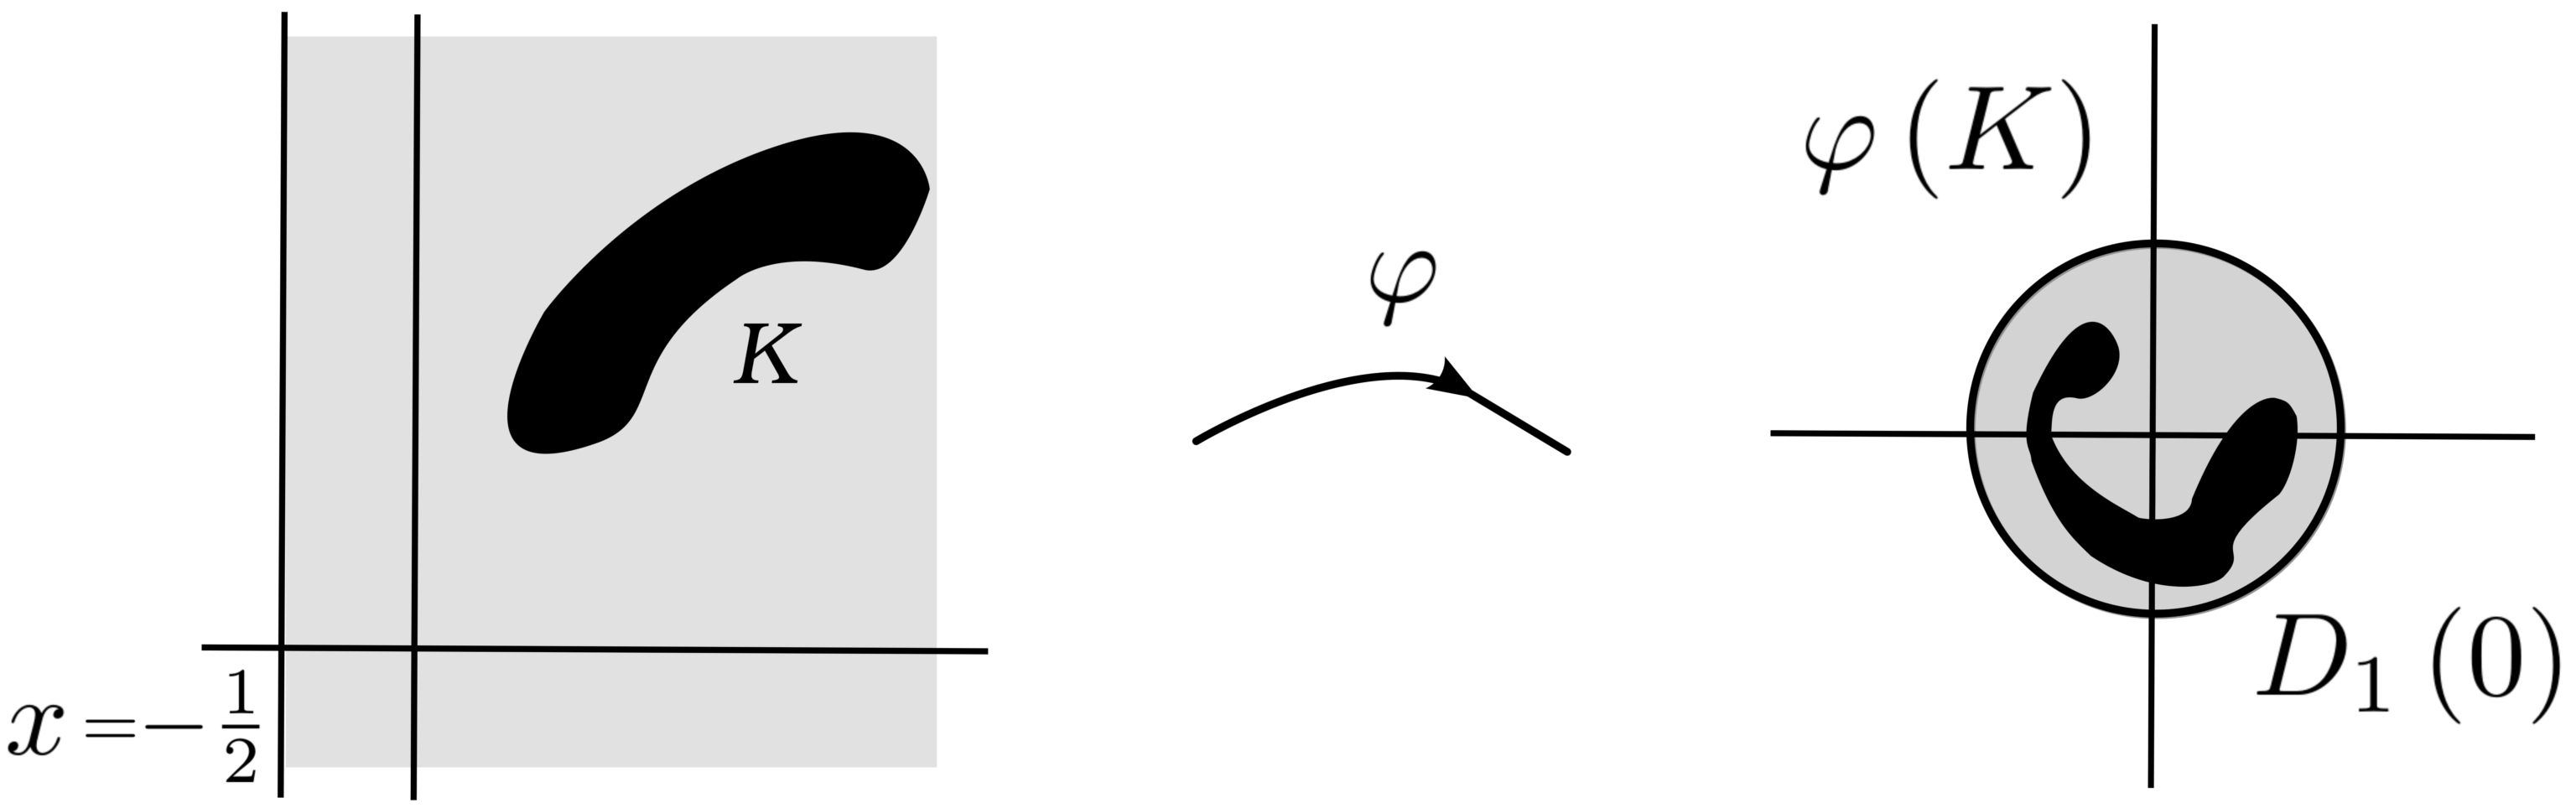
\includegraphics{2.png}
\end{center}

\bigskip

\textbf{Definição 3.6 \ }Sejam $(  c_{m})  _{m\in%
%TCIMACRO{\U{2115} }%
%BeginExpansion
\mathbb{N}
%EndExpansion
}$ uma sequência de números complexos

e $\zeta\in%
%TCIMACRO{\U{2102} }%
%BeginExpansion
\mathbb{C}
%EndExpansion
.$ Chama-se \textit{série de potências }(de $%
%TCIMACRO{\U{2102} }%
%BeginExpansion
\mathbb{C}
%EndExpansion
$ em $%
%TCIMACRO{\U{2102} }%
%BeginExpansion
\mathbb{C}
%EndExpansion
$) \textit{com coeficientes}

$c_{m}$ \textit{em volta de }$\zeta$ à série de funções de
termo geral $f_{m\text{ }}$ sendo

\ \ \ \ \ \ \ \ \ \ \ \ \ \ \ $f_{m}(  z)  =c_{m}(
z-\zeta)  ^{m}$ \ \ $\forall$ \ $m\in%
%TCIMACRO{\U{2115} }%
%BeginExpansion
\mathbb{N}
%EndExpansion
,$ \ \ $\forall$ \ $z\in%
%TCIMACRO{\U{2102} }%
%BeginExpansion
\mathbb{C}
%EndExpansion
.$

Indicamos esta série pela notação

\ \ \ \ \ \ \ \ \ \ \ \ \ \ \ \ \ \ \ \ \ \ $\underset{m=0}{\overset{\infty
}{\sum}}c_{m}(  z-\zeta)  ^{m}$ \ \ \ \ \ \ \ \ ou
\ \ \ \ \ \ \ \ $\sum c_{m}(  z-\zeta)  ^{m}.$

\bigskip

Dada uma série de potências

\bigskip$(  (  \ast)  )  $
\ \ \ \ \ \ \ \ \ \ \ \ \ \ \ \ \ \ \ \ \ \ \ \ \ \ \ \ \ \ \ \ \ $\overset
{\infty}{\underset{m=0}{\sum}}c_{m}(  z-\zeta)  ^{m}$

vamos estudar o conjunto $X$ dos $z\in%
%TCIMACRO{\U{2102} }%
%BeginExpansion
\mathbb{C}
%EndExpansion
$ tais que $(  (  \ast)  )  $ é convergente em

$z$ e se $f$ é a soma da série $(  (  \ast)  )
$ vamos estudar as propriedades da

função $f.$ Vamos ver que a natureza deste conjunto $X$ é muito simples,

essencialmenrte $X$ é um "disco". Em primeiro lugar, para simplificar e

unificar a linguagem, vamos ampliar o nosso conceito de disco,

admitindo discos de raio nulo e de raio $+\infty.$

$\ \ \ \ \ \ \ \ \overline{D}_{0}(  \zeta)  =\left\{
\zeta\right\}  $ \ \ , \ \ $\overline{D}_{\infty}(  \zeta)
=D_{\infty}(  \zeta)  =%
%TCIMACRO{\U{2102} }%
%BeginExpansion
\mathbb{C}
%EndExpansion
$ \ \ , \ \ $D_{0}(  \zeta)  =\varnothing$

\bigskip

A afirmação acima segundo a qual $X$ é essencialmente um disco

significa que

\ \ \ \ \ \ \ \ \ \ \ \ \ \ \ \ \ \ \ \ \ \ \ \ \ \ \ $D_{r}(
\zeta)  \subset X\subset\overline{D}_{r}(  \zeta)  $

para algum $r$ tal que $0\leq r\leq+\infty,$ isto é, $X$ pode ser igual a
$%
%TCIMACRO{\U{2102} }%
%BeginExpansion
\mathbb{C}
%EndExpansion
$ ou $\left\{  \zeta\right\}  $ ou

$X$ é a reunião de um disco aberto (de raio positivo) com parte de sua

fronteira que eventualmente pode ser a fronteira toda, e, neste caso, $X$

é um disco fechado de raio positivo. Observar que sempre $X\neq
\varnothing$ pois

$\zeta\in X$.\\

Dada a série de potências\\

$(  (  \ast)  )  $%
\ \ \ \ \ \ \ \ \ \ \ \ \ \ \ \ \ \ \ \ \ \ \ \ \ \ \ $\underset{m=0}%
{\overset{\infty}{\sum}}c_{m}(  z-\zeta)  ^{m}$\\

consideremos o seguinte conjunto:

\bigskip

\textsc{I}$=\{r\in%
%TCIMACRO{\U{211d} }%
%BeginExpansion
\mathbb{R}
%EndExpansion
_{+}$ $|$ a série de termos não negativos $\overset{\infty}%
{\underset{m=0}{\sum}}\left\vert c_{m}\right\vert r^{m}$ é convergente$\}$.


\bigskip

É claro que \textsc{I} é não vazio pois $0\in$ \textsc{I} ,
além disso se $r\in$\textsc{I} e $r>0,$ então

$\left[  0,r\right]  \subset$\textsc{I}, o que mostra que \textsc{I} é um
intervalo contido em $%
%TCIMACRO{\U{211d} }%
%BeginExpansion
\mathbb{R}
%EndExpansion
_{+}.$ Este intervalo

é fechado à esquerda pois $0\in$\textsc{I} e pode ser aberto ou
fechado à direita,

pode ser limitado ou não e pode ser reduzido a $\left\{  0\right\}  .$ Em
qualquer caso

seja

\ \ \ \ \ \ \ \ \ \ \ \ \ \ \ \ \ \ \ \ \ \ \ \ \ \ \ \ \ \ \ \ \ \ \ \ \ \ \ $\rho
:=\sup$ \textsc{I},

então $\rho$ é um elemento de $\overline{%
%TCIMACRO{\U{211d} }%
%BeginExpansion
\mathbb{R}
%EndExpansion
}_{+}:=\left[  0,+\infty\right]  ,$ finito ou infinito, eventualmente

nulo; é chamado \textit{raio de convergência da série de
potências }$(  (  \ast)  )  $ e,

quando $\rho>0,$ o disco $D_{\rho}(  \zeta)  $ é chamado
\textit{disco de convergência da série}

\textit{de potências }$(  (  \ast)  )  .$

\bigskip

\textbf{Lema 3.7 \ }(Abel) \ \textit{Sejam }$r$\textit{\ e }$s$%
\textit{\ \ dois números reais tais que }$0<r<s$\textit{\ }

\textit{e seja}

\textit{\bigskip\ }$(  (  \ast)  )  $
\ \ \ \ \ \ \ \ \ \ \ \ \ \ \ \ $\underset{m=0}{\overset{\infty}{\sum}}%
c_{m}(  z-\zeta)  ^{m}$

\textit{uma série de potências. Se existe }$M>0$\textit{\ tal que}

\ \ \ \ \ \ \ \ \ \ \ \ \ \ \ \ \ \ \ \ \ \ \ \ \ $\left\vert c_{m}\right\vert
s^{m}\leq M$ \ \textit{para cada} \ $m\in%
%TCIMACRO{\U{2115} }%
%BeginExpansion
\mathbb{N}
%EndExpansion
,$

\textit{então a série }$(  (  \ast)  )
$\textit{\ converge uniformemente e absolutamente em} $\ \overline{D}%
_{r}(  \zeta)  .$

\bigskip

\textbf{Prova \ }De fato, para cada $z\in\overline{D}_{r}(  \zeta)
$ temos $\left\vert z-\zeta\right\vert \leq r,$ donde resulta

$\ \ \ \ $

$\ \ \ \left\vert c_{m}\right\vert \left\vert z-\zeta\right\vert ^{m}%
\leq\left\vert c_{m}\right\vert r^{m}=\left\vert c_{m}\right\vert s^{m}(
\frac{r}{s})  ^{m}\leq M(  \frac{r}{s})  ^{m},$ \ para cada
\ $m\in%
%TCIMACRO{\U{2115} }%
%BeginExpansion
\mathbb{N}
%EndExpansion
$

\bigskip

portanto aplicando a Prop. 3.5 (com $b_{m}:=M(  \frac{r}{s})  ^{m}%
$) resulta que $(  (  \ast)  )  $ \ é

uniformemente e absolutamente convergente em $\overline{D}_{r}(
\zeta)  $ pois

\bigskip\ \ \ \ \ \ \ \ \ \ \ \ \ \ \ \ \ \ \ \ \ \ \ \ \ \ \ $\overset
{\infty}{\underset{m=0}{\sum}}b_{m}=\underset{m=0}{\overset{\infty}{\sum}%
}M(  \frac{r}{s})  ^{m}=%
%TCIMACRO{\QDOVERD{.}{.}{Ms}{s-r}}%
%BeginExpansion
\genfrac{.}{.}{}{0}{Ms}{s-r}%
%EndExpansion
<\infty.$ \ $\square$

\bigskip

O resultado seguinte\ mostra duas propriedades do raio de convergência

que o caracterizam quando é um número real positivo.

\bigskip

\textbf{Proposição 3.8 \ }Seja $\rho\in%
%TCIMACRO{\U{211d} }%
%BeginExpansion
\mathbb{R}
%EndExpansion
_{+}^{\ast}$ \textit{o raio de convergência de uma série de}

\textit{potências}

$(  (  \ast)  )  $
\ \ \ \ \ \ \ \ \ \ \ \ \ \ \ \ \ \ \ \ \ \ \ \ \ \ \ $\overset{\infty
}{\underset{m=0}{\sum}}c_{m}(  z-\zeta)  ^{m}$

\textit{então}:

(a) \ \textit{Para todo }$r\in\left]  0,\rho\right[  ,$ \textit{a série
}$(  (  \ast)  )  $ \textit{é uniformemente e
absolutamente}

\textit{convergente em }$\overline{D}_{r}(  \zeta)  .$

(b) \ \textit{Para todo }$z_{0}\in%
%TCIMACRO{\U{2102} }%
%BeginExpansion
\mathbb{C}
%EndExpansion
$ \ \textit{tal que }$\left\vert z_{0}-\zeta\right\vert >\rho,$ \textit{a
série }$(  (  \ast)  )  $ \ \textit{é divergente
}

\textit{em }$z_{0}.$

\textit{Reciprocamente, se }$\rho\in%
%TCIMACRO{\U{211d} }%
%BeginExpansion
\mathbb{R}
%EndExpansion
_{+}^{\ast}$ \textit{satisfaz }(a) \textit{e }(b) \textit{então }$\rho$
\textit{é o raio de conver-}

\textit{gência de }$(  (  \ast)  )  .$

\bigskip

\textbf{Prova \ }(a) \ Fixado $r\in\left]  0,\rho\right[  ,$ seja $s$ tal que
$r<s<\rho,$ então por definição

de raio de convergência, a série

\ \ \ \ \ \ \ \ \ \ \ \ \ \ \ \ \ \ \ \ \ \ \ \ \ \ \ \ \ \ \ \ \ \ \ \ \ \ \ \ $\underset
{n\geq0}{\sum}\left\vert c_{n}\right\vert s^{n}$

é convergente, donde para cada $m\in%
%TCIMACRO{\U{2115} }%
%BeginExpansion
\mathbb{N}
%EndExpansion
,$ resulta

\ \ \ \ \ \ \ \ \ \ \ \ \ \ \ \ \ \ \ \ \ \ \ \ $\left\vert c_{m}\right\vert
s^{m}\leq\underset{n\geq0}{\sum}\left\vert c_{n}\right\vert s^{n}=:M<+\infty$

\bigskip

o que pelo Lema 3.7 prova a asserção.

(b) \ Fixado $z_{0}\in%
%TCIMACRO{\U{2102} }%
%BeginExpansion
\mathbb{C}
%EndExpansion
$ tal que $\left\vert z_{0}-\zeta\right\vert >\rho$ arbitrário, vamos
provar que:

\bigskip

(3.8.1) \ Para cada $\nu\in%
%TCIMACRO{\U{2115} }%
%BeginExpansion
\mathbb{N}
%EndExpansion
$ existe $m_{\nu}\in%
%TCIMACRO{\U{2115} }%
%BeginExpansion
\mathbb{N}
%EndExpansion
$ tal que $\left\vert c_{m_{\nu}}\right\vert \left\vert z-\zeta\right\vert
^{m_{\nu}}>\nu$

\bigskip

De fato, suponhamos por absurdo que (3.8.1) é falsa, então existe

$\nu_{0}\in%
%TCIMACRO{\U{2115} }%
%BeginExpansion
\mathbb{N}
%EndExpansion
$ tal que

\bigskip

(3.8.2) \ \ \ \ \ \ \ \ \ \ \ \ \ \ \ \ \ $\left\vert c_{m}\right\vert
\left\vert z_{0}-\zeta\right\vert ^{m}\leq\nu_{0}$ \ \ para cada $m\in%
%TCIMACRO{\U{2115} }%
%BeginExpansion
\mathbb{N}
%EndExpansion
.$

\bigskip

Escolhendo um número real $t$ tal que $\rho<t<\left\vert z_{0}%
-\zeta\right\vert ,$ pelo Lema 3.7

(os reais $r$ e $s$ daquele Lema substituídos por $t$ e $\left\vert
z_{0}-\zeta\right\vert $ \ respectiva-

mente), de (3.8.2) resultaria que $(  (  \ast)  )  $
seria absolutamente convergente

em $\overline{D}_{t}(  \zeta)  $ e como $\xi=\zeta+t\in\overline
{D}_{t}(  \zeta)  ,$ em particular a série numérica

$\sum c_{m}(  \xi-\zeta)  ^{m}$ seia absolutamente convergente,
isto é

\bigskip\ \ \ \ \ \ \ \ \ \ \ \ \ \ \ \ \ \ \ \ \ \ $\underset{m\geq0}{\sum
}\left\vert c_{m}\right\vert \left\vert \xi-\zeta\right\vert ^{m}%
=\underset{m\geq0}{\sum}\left\vert c_{m}\right\vert t^{m}$ \ \ é convergente,

o que é absurdo pois $t>\rho=$ raio de convergência de $(
(  \ast)  )  .$ Desta

forma fica provada a asserção (3.8.1).

Observemos finalmente que

\bigskip

(3.8.3) \ \ \ \ \ \ \ $\underset{m\rightarrow\infty}{\lim}\left\vert
c_{m}\right\vert \left\vert z_{o}-\zeta\right\vert ^{m}=0\iff\underset
{m\rightarrow\infty}{\lim}c_{m}(  z_{0}-\zeta)  ^{m}=0$

\bigskip

e (3.8.1) prova que a primeira das asserções (3.8.3) é falsa, portanto

a segunda também é falsa, o que mostra que a série
\textit{numérica}

$\sum c_{m}(  z_{0}-\zeta)  ^{m}$ não é convergente e
portanto é divergente.

Inversamente, vamos mostrar que se $\rho\in%
%TCIMACRO{\U{211d} }%
%BeginExpansion
\mathbb{R}
%EndExpansion
_{+}^{\ast}$ satisfaz (a) e (b) então $\rho$

é o raio de convergência de $(  (  \ast)  )  ,$
isto é, $\rho=\sup$ \textsc{I}. De fato, seja

$\rho_{\ast}=\sup$ \textsc{I }então é claro que $\rho_{\ast}<\rho$
é falso [pois de $\ \rho_{\ast}<r<\rho$ resulta

($\rho$ verifica (a) por hipótese!) que $\sum\left\vert c_{m}\right\vert
r^{m}<+\infty$ \ portanto $r\in$\textsc{I } logo

$\rho_{\ast}=\sup$ \textsc{I}$<r\in$ \textsc{I}, o que seria ridículo],
logo $\rho\leq\rho_{\ast}.$ Por outro lado, se

fosse $\rho<\rho_{\ast},$ como $\rho_{\ast}$ é raio de convergência de
$(  (  \ast)  )  $ por hipótese,

o argumento que usamos na prova de (a) [aplicado agora ao par

$(  \rho,\rho^{\ast})  $ que substitui o par $(
r,\rho)  $] \ mostraria que se $\rho<s<\rho^{\ast}$ \ então

$\sum\left\vert c_{m}\right\vert s^{m}<+\infty.$ Portanto, \ $\forall$
\ $z_{0}\in%
%TCIMACRO{\U{2102} }%
%BeginExpansion
\mathbb{C}
%EndExpansion
$ tal que $\left\vert z_{0}-\zeta\right\vert =1,$ a série

$\sum c_{m}(  z_{0}-\zeta)  ^{m}$seria absolutamente convergente
(i.e. $(  (  \ast)  )  $ seria A.C.

em $z_{0}$), o que é absurdo pois por hipótese $\rho$ satisfaz (b).
\ $\square$

\bigskip

\textbf{Corolário 3.9} \ \textit{Seja }$\rho\in%
%TCIMACRO{\U{211d} }%
%BeginExpansion
\mathbb{R}
%EndExpansion
_{+}^{\ast}$\textit{\ o raio de convergência de uma série de }

\textit{potências}

$(  (  \ast)  )  $
\ \ \ \ \ \ \ \ \ \ \ \ \ \ \ \ \ \ \ \ \ \ $\underset{m\geq0}{\sum}%
c_{m}(  z-\zeta)  ^{m}$

\textit{Se a série }$(  (  \ast)  )  $
\textit{converge em }$z_{0}\in%
%TCIMACRO{\U{2102} }%
%BeginExpansion
\mathbb{C}
%EndExpansion
,$\textit{\ então }$\sigma:=\left\vert z_{0}-\zeta\right\vert \leq\rho,$
\textit{em}

\textit{consequência, a série }$(  (  \ast)  )
$ \textit{é uniformemente e absolutamente }

\textit{convergente \ em }$\overline{D}_{s}(  \zeta)
,$\textit{\ para cada }$s\in\left]  0,\sigma\right[  .$

\bigskip

\textbf{Prova \ }Suponhamos por absurdo que $\sigma=\left\vert z_{0}%
-\zeta\right\vert >\rho,$ então pela Prop.

3.8.(b) a série $\sum c_{m}(  z_{0}-\zeta)  ^{m}$ seria
divergente contra o suposto, logo

$\sigma\leq\rho.$ Se $s\in\left]  0,\sigma\right[  ,$ como $\sigma\leq\rho$
resulta $s\in\left]  0,\rho\right[  $ e então pela Prop.

3.8. (a) resulta que $(  (  \ast)  )  $ é
uniformemente e absolutamente convergente

em $\overline{D}_{s}(  \zeta)  .$ \ $\square$

\bigskip

Completamos a informação sobre o disco de convergência de uma

série de potências com um resultdo que expressa seu raio em função

dos coeficientes.

\bigskip

\textbf{Proposição 3.10 \ }(Hadamard) \ \textit{O raio de
convergência }$\rho$\textit{\ de uma }

\textit{série potências}

\ \ \ \ \ \ \ \ \ \ \ \ \ \ \ \ \ \ \ \ \ \ \ \ \ \ \ \ \ \ $\sum c_{m}(
z-\zeta)  ^{m}$

\bigskip

\textit{é dado pela expressão}

\ \ \ \ \ \ \ \ \ $\rho=%
%TCIMACRO{\QDOVERD{.}{.}{1}{\underset{m\rightarrow\infty}{\lim\sup}\left\vert
%c_{m}\right\vert ^{1/m}}}%
%BeginExpansion
\genfrac{.}{.}{}{0}{1}{\underset{m\rightarrow\infty}{\lim\sup}\left\vert
c_{m}\right\vert ^{1/m}}%
%EndExpansion
$ \ \ \ (com as convenções: $%
%TCIMACRO{\QDOVERD{.}{.}{1}{+\infty}}%
%BeginExpansion
\genfrac{.}{.}{}{0}{1}{+\infty}%
%EndExpansion
=0$ e $%
%TCIMACRO{\QDOVERD{.}{.}{1}{0}}%
%BeginExpansion
\genfrac{.}{.}{}{0}{1}{0}%
%EndExpansion
=+\infty$).

\bigskip

\textbf{Prova \ }Sejam $\Lambda:=\underset{m\rightarrow\infty}{\lim\sup
}\left\vert c_{m}\right\vert ^{1/m}$ \ e \ $\lambda=1/\Lambda,$ \ vamos
mostrar que

(3.10.1)
\ \ \ \ \ \ \ \ \ \ \ \ \ \ \ \ \ \ \ \ \ \ \ \ \ \ \ \ \ \ \ \ \ \ \ \ $\lambda
=\rho$

\bigskip

\textbf{Caso 1}: \ \ \ \ $0<\Lambda<+\infty$

Se $r\in%
%TCIMACRO{\U{211d} }%
%BeginExpansion
\mathbb{R}
%EndExpansion
_{+}^{\ast}$ então

$\ \ \ \ \ \ \ \ \ \ \ r<\lambda=%
%TCIMACRO{\QDOVERD{.}{.}{1}{\Lambda}}%
%BeginExpansion
\genfrac{.}{.}{}{0}{1}{\Lambda}%
%EndExpansion
\iff r\Lambda=r\underset{m\rightarrow\infty}{\limsup}\left\vert c_{m}%
\right\vert ^{1/m}=\underset{m\rightarrow\infty}{\limsup}\sqrt[m]{\left\vert
c_{m}\right\vert r^{m}}<1$

\bigskip

e esta última desigualdade implica, pelo teste da raiz, que $\sum
\left\vert c_{m}\right\vert r^{m}$

converge e então por definição de $\rho$ resulta $r\leq\rho,$
portanto provamos

que

\ \ \ \ \ \ \ \ \ \ \ \ \ \ \ \ $r\in%
%TCIMACRO{\U{211d} }%
%BeginExpansion
\mathbb{R}
%EndExpansion
_{+}^{\ast}$ \ \ \ \ \ e \ \ \ \ \ $r<\lambda$ \ \ \ \ $\implies$
\ \ \ \ $r\leq\rho$

o que é equivalente a

\bigskip

(3.10.2)
\ \ \ \ \ \ \ \ \ \ \ \ \ \ \ \ \ \ \ \ \ \ \ \ \ \ \ \ \ \ \ \ $\lambda
\leq\rho$.

\bigskip

Por outro lado, se $r\in%
%TCIMACRO{\U{211d} }%
%BeginExpansion
\mathbb{R}
%EndExpansion
_{+}^{\ast}$ temos:

\ \ \ \ \ \ \ \ \ \ \ \ \ \ \ \ \ $r>\lambda=%
%TCIMACRO{\QDOVERD{.}{.}{1}{\Lambda}}%
%BeginExpansion
\genfrac{.}{.}{}{0}{1}{\Lambda}%
%EndExpansion
\iff r\Lambda=\underset{m\rightarrow\infty}{\limsup}\sqrt[m]{\left\vert
c_{m}\right\vert r^{m}}>1$

e esta última desigualdade, de novo pelo teste da raiz, implica que

$\sum\left\vert c_{m}\right\vert r^{m}$ \ é divergente \ e então por
definição de $\rho$ resulta $r\geq\rho,$

portanto provamos que

\ \ \ \ \ \ \ \ \ \ \ \ \ \ \ \ \ \ \ \ \ $r\in%
%TCIMACRO{\U{211d} }%
%BeginExpansion
\mathbb{R}
%EndExpansion
_{+}^{\ast}$ \ \ e \ \ $r>\lambda\implies r\geq\rho$

o que é equivalente a

\bigskip

(3.10.3) \ \ \ \ \ \ \ \ \ \ \ \ \ \ \ \ \ \ \ \ \ \ \ \ \ \ \ \ $\lambda
\geq\rho.$

\bigskip

De (3.10.2) e (3.10.3) resulta (3.10.1)

\textbf{Caso 2:} \ \ \ \ \ \ $\Lambda=0$

Se $\Lambda=\underset{m\rightarrow\infty}{\limsup}\left\vert c_{m}\right\vert
^{1/m}=0$ \ então é claro que

\bigskip

\ \ \ \ \ \ \ \ \ \ \ \ \ \ \ \ $\underset{m\rightarrow\infty}{\limsup
}\sqrt[m]{\left\vert c_{m}\right\vert r^{m}}=r\cdot\Lambda=0<1$ \ \ $\forall$
\ $r>0$

o que pelo teste das raíz \ implica que $\sum\left\vert c_{m}\right\vert
r^{m}$ converge para cada

$r>0,$ donde $\rho=+\infty=%
%TCIMACRO{\QDOVERD{.}{.}{1}{0}}%
%BeginExpansion
\genfrac{.}{.}{}{0}{1}{0}%
%EndExpansion
=%
%TCIMACRO{\QDOVERD{.}{.}{1}{\Lambda}}%
%BeginExpansion
\genfrac{.}{.}{}{0}{1}{\Lambda}%
%EndExpansion
=\lambda$.

\textbf{Caso 3:} \ $\Lambda=+\infty$

Se $\ \Lambda=\underset{m\rightarrow\infty}{\limsup}\left\vert c_{m}%
\right\vert ^{1/m}=+\infty,$ \ \ então é claro que

\ \ \ \ \ \ \ \ \ \ \ \ \ \ $\underset{m\rightarrow\infty}{\limsup}%
\sqrt[m]{\left\vert c_{m}\right\vert r^{m}}=r\cdot\Lambda=r(
+\infty)  =+\infty>1$ \ \ $\forall$ \ $r>0$

donde pelo teste da raíz resulta que $\sum\left\vert c_{m}\right\vert
r^{m}$ é divergente para cada

$\bigskip$

$r>0$ \ e em consequência $\rho=0=%
%TCIMACRO{\QDOVERD{.}{.}{1}{+\infty}}%
%BeginExpansion
\genfrac{.}{.}{}{0}{1}{+\infty}%
%EndExpansion
=%
%TCIMACRO{\QDOVERD{.}{.}{1}{\Lambda}}%
%BeginExpansion
\genfrac{.}{.}{}{0}{1}{\Lambda}%
%EndExpansion
=\lambda.$ \ $\square$

\bigskip

\textbf{Observação \ }Até agora não fizemos nenhuma
referência ao comporta-

mento de uma série de potências na fronteira (circunferência) do seu

disco de convergência e a razão disto é que este comportamento é

muito variado e não pode ser descrito de forma simples. Este fato torna

a questão difícil e como é completamente irrelevante para os nossos

propósitos é natural deixa-la de lado num texto introdutório como este.

Vamos ilustrar com um exemplo simples o comportamento difícil de uma

série de potências na fronteira do seu disco de convergência.

Nas hipóteses do Corol. 3.9 isto é, se $\rho\in%
%TCIMACRO{\U{211d} }%
%BeginExpansion
\mathbb{R}
%EndExpansion
_{+}^{\ast}$ e a série $\sum c_{m}(  z-\zeta)  ^{m}$

\textit{converge no ponto }$z_{0}\in%
%TCIMACRO{\U{2102} }%
%BeginExpansion
\mathbb{C}
%EndExpansion
,$ já vimos que $r=\left\vert z_{0}-\zeta\right\vert \leq\rho.$ No caso

$r=\left\vert z_{0}-\zeta\right\vert =\rho,$ não pertinentes as
observações seguintes:

(1%
%TCIMACRO{\U{ba}}%
%BeginExpansion
${{}^o}$%
%EndExpansion
) \ A série $\sum c_{m}(  z-\zeta)  ^{m}$ não é
necessáriamente absolutamente

convergente em $z_{0}$ (i.e. $\sum\left\vert c_{m}\right\vert \left\vert
z_{0}-\zeta\right\vert ^{m}$ pode ser divergente).

(2%
%TCIMACRO{\U{ba}}%
%BeginExpansion
${{}^o}$%
%EndExpansion
) \ Se $\left\vert z_{1}-\zeta\right\vert =r=\rho$ \ e \ $z_{1}\neq z_{0},$ a
série $\sum c_{m}(  z-\zeta)  ^{m}$ não é necessária

mente convergente \ em $z_{1}$ (isto é, pode existir um ponto $z_{1}%
\in\partial\overline{D}_{\rho}(  \zeta)  $ \ tal

que não existe o limite $\underset
{m\rightarrow\infty}{\lim}\underset{k=0}{\overset{m}{\sum}}c_{k}(
z_{1}-\zeta)  ^{k}$).


% IMAGEM 3

\begin{center}
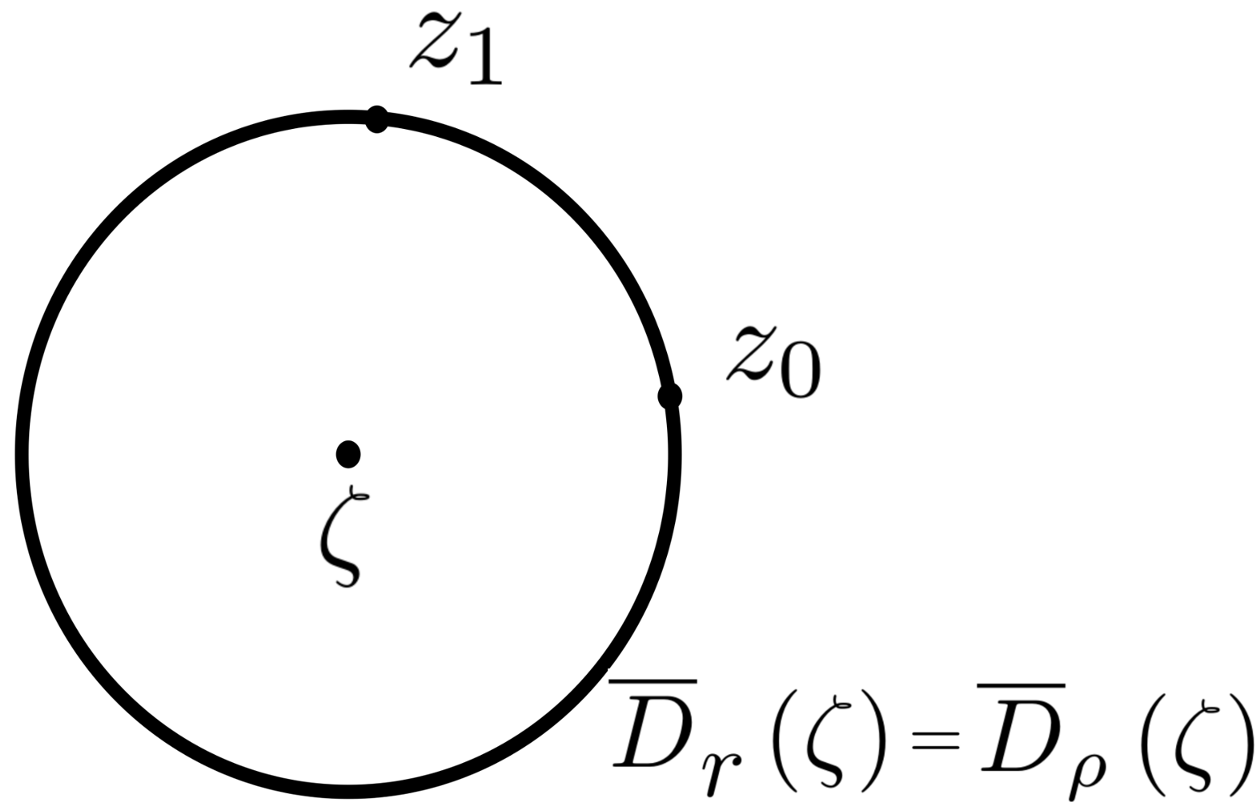
\includegraphics{3.png}
\end{center}



Para provar estas duas asserções vamos considerar o exemplo seguinte

\bigskip

(S) \ \ \ \ \ \ \ \ \ \ \ \ \ \ \ \ \ \ \ \ \ \ \ \ \ \ $\overset{\infty
}{\underset{m=1}{\sum}}%
%TCIMACRO{\QDOVERD{.}{.}{1}{m}}%
%BeginExpansion
\genfrac{.}{.}{}{0}{1}{m}%
%EndExpansion
z^{m}$

\bigskip

e o resultado seguinte (\cite{R1}, Teor. 3.44]): \textit{Suponhamos que o raio de }

\textit{convergência da série }$\sum c_{m}z^{m}$ \textit{seja }%
$1$,\textit{\ que }$c_{0}\geq c_{1}\geq$ $\ldots$ $\geq c_{m}\geq
c_{m+1}\ldots$

\textit{e que }$\underset{m\rightarrow\infty}{\lim}c_{m}=0.$ \textit{Então
}$\sum c_{m}z^{m}$\textit{\ converge em todos os pontos }$z$ \textit{tais que}

$\left\vert z\right\vert =1,$ \textit{com a possível exceção de
}$z=1.$

Pela fórmula de Hadarmard (Prop. 3.10), o raio de convergência da série

(S) é

\ \ \ \ \ \ \ \ \ \ \ \ \ \ \ \ \ \ \ $\rho=%
%TCIMACRO{\QDOVERD{.}{.}{1}{\underset{m\rightarrow\infty}{\limsup}\sqrt[m]%
%{1/m}}}%
%BeginExpansion
\genfrac{.}{.}{}{0}{1}{\underset{m\rightarrow\infty}{\limsup}\sqrt[m]{1/m}}%
%EndExpansion
=%
%TCIMACRO{\QDOVERD{.}{.}{1}{\underset{m\rightarrow\infty}{\lim}\sqrt[m]{1/m}}}%
%BeginExpansion
\genfrac{.}{.}{}{0}{1}{\underset{m\rightarrow\infty}{\lim}\sqrt[m]{1/m}}%
%EndExpansion
=1$

o que mostra que a série (S) verifica as hipóteses do resultado acima e

portanto (S) converge em todos os pontos $z\in%
%TCIMACRO{\U{2102} }%
%BeginExpansion
\mathbb{C}
%EndExpansion
$ tais que $\left\vert z\right\vert =1$ salvo em

$z=1,$ onde evidentemente (S) não converge. Resulta então que para cada

$z\in%
%TCIMACRO{\U{2102} }%
%BeginExpansion
\mathbb{C}
%EndExpansion
,\left\vert z\right\vert =1$ e $z\neq1,$ (S) converge em $z$ porém (S)
não é absolutamente

convergente em $z$ (pois $\sum%
%TCIMACRO{\QDOVERD{.}{.}{1}{m}}%
%BeginExpansion
\genfrac{.}{.}{}{0}{1}{m}%
%EndExpansion
\left\vert z\right\vert ^{m}=\sum%
%TCIMACRO{\QDOVERD{.}{.}{1}{m}}%
%BeginExpansion
\genfrac{.}{.}{}{0}{1}{m}%
%EndExpansion
=+\infty$), o que prova \ a asserção

(1%
%TCIMACRO{\U{ba}}%
%BeginExpansion
${{}^o}$%
%EndExpansion
). Por outro lado, tomando $z_{0}=i$ e $z_{1}=1$ na série (S), o resultado acima

prova a asserção (2%
%TCIMACRO{\U{ba}}%
%BeginExpansion
${{}^o}$%
%EndExpansion
).

\bigskip

O resultado seguinte constitui a parte essencial da prova de que toda

função analítica é holomorfa, o que será demonstrado no
capítulo 4.

\bigskip

\textbf{Lema 3.11} \ \textit{Se }$\rho\in\overline{%
%TCIMACRO{\U{211d} }%
%BeginExpansion
\mathbb{R}
%EndExpansion
}_{+}^{\ast}$ \textit{é o raio de convergência de uma série de
po-}

\textit{tências}

(S) \ \ \ \ \ \ \ \ \ \ \ \ \ \ \ \ \ \ \ \ \ \ \ $\underset{m=0}%
{\overset{\infty}{\sum}}c_{m}(  z-\zeta)  ^{m},$

\textit{então a série de potências derivada:}

(S$^{\prime}$) \ \ \ \ \ \ \ \ \ \ \ \ \ \ \ \ \ \ \ \ \ $\overset{\infty
}{\underset{m=1}{\sum}}mc_{m}(  z-\zeta)  ^{m-1}$

\textit{também tem raio de convergência }$\rho.$

\bigskip

\textbf{Prova \ } Segue diretamente da Proposição 3.10. $\square$

\bigskip

Como aplicação importante do breve resumo precedente sobre séries

de potências, encerramos este capítulo com a definição e
algumas das

propriedades mais importantes da funçào exponencial.

\bigskip

\textbf{Proposição 3.12 \ }\textit{A série de potências }

\ \ \ \ \ \ \ \ \ \ \ \ \ \ \ \ \ \ \ \ \ \ \ \ \ \ \ \ \ \ \ \ \ \ \ \ $\exp
(  z)  =\underset{m\geq0}{\sum}%
%TCIMACRO{\QDOVERD{.}{.}{1}{m!}}%
%BeginExpansion
\genfrac{.}{.}{}{0}{1}{m!}%
%EndExpansion
z^{m}$

\textit{é absolutamente convergente em }$%
%TCIMACRO{\U{2102} }%
%BeginExpansion
\mathbb{C}
%EndExpansion
$ \textit{e uniformemente convergente em}

$\overline{D}_{r}(  0)  $ \textit{para cada \ }$r\in%
%TCIMACRO{\U{211d} }%
%BeginExpansion
\mathbb{R}
%EndExpansion
_{+}^{\ast}.$

\bigskip

\textbf{Prova \ }Dado $z_{0}\in%
%TCIMACRO{\U{2102} }%
%BeginExpansion
\mathbb{C}
%EndExpansion
$ arbitrário, a série $\underset{m\geq0}{\sum}%
%TCIMACRO{\QDOVERD{.}{.}{1}{m!}}%
%BeginExpansion
\genfrac{.}{.}{}{0}{1}{m!}%
%EndExpansion
\left\vert z_{0}\right\vert ^{m}$ converge pelo teste

da razão pois

\ \ \ \ \ \ \ \ \ \ \ \ \ \ \ \ \ \ \ $\underset{m\rightarrow\infty}{\limsup
}\left[
%TCIMACRO{\QDOVERD{.}{.}{\left\vert z_{0}\right\vert ^{m+1}}{(
%m+1)  !}}%
%BeginExpansion
\genfrac{.}{.}{}{0}{\left\vert z_{0}\right\vert ^{m+1}}{(  m+1)  !}%
%EndExpansion
\cdot%
%TCIMACRO{\QDOVERD{.}{.}{m!}{\left\vert z_{0}\right\vert ^{m}}}%
%BeginExpansion
\genfrac{.}{.}{}{0}{m!}{\left\vert z_{0}\right\vert ^{m}}%
%EndExpansion
\right]  =\underset{m\rightarrow\infty}{\lim}%
%TCIMACRO{\QDOVERD{.}{.}{\left\vert z_{0}\right\vert }{m+1}}%
%BeginExpansion
\genfrac{.}{.}{}{0}{\left\vert z_{0}\right\vert }{m+1}%
%EndExpansion
=0<1$

\bigskip

o que prova que $\underset{m\geq0}{\sum}%
%TCIMACRO{\QDOVERD{.}{.}{1}{m!}}%
%BeginExpansion
\genfrac{.}{.}{}{0}{1}{m!}%
%EndExpansion
z^{m\text{ }}$ é absolutamente convergente em $%
%TCIMACRO{\U{2102} }%
%BeginExpansion
\mathbb{C}
%EndExpansion
.$ Dado

$r\in%
%TCIMACRO{\U{211d} }%
%BeginExpansion
\mathbb{R}
%EndExpansion
_{+}^{\ast}$ arbitrário, para cada $z\in\overline{D}_{r}(  0)
$ temos $\left\vert z\right\vert \leq r,$ donde

\bigskip

(3.12.1) \ \ \ \ \ \ \ \ \ \ \ \ \ \ \ \ $%
%TCIMACRO{\QDOVERD{.}{.}{1}{m!}}%
%BeginExpansion
\genfrac{.}{.}{}{0}{1}{m!}%
%EndExpansion
\left\vert z\right\vert ^{m}\leq%
%TCIMACRO{\QDOVERD{.}{.}{1}{m!}}%
%BeginExpansion
\genfrac{.}{.}{}{0}{1}{m!}%
%EndExpansion
r^{m}$ \ \ $\forall$ \ $z\in\overline{D}_{r}(  0)  $ \ e
\ $\forall$ \ $m\in%
%TCIMACRO{\U{2115} }%
%BeginExpansion
\mathbb{N}
%EndExpansion
$

\bigskip

Como $\sum%
%TCIMACRO{\QDOVERD{.}{.}{1}{m!}}%
%BeginExpansion
\genfrac{.}{.}{}{0}{1}{m!}%
%EndExpansion
z^{m}$ é absolutamente convergente em $%
%TCIMACRO{\U{2102} }%
%BeginExpansion
\mathbb{C}
%EndExpansion
,$ resulta que a

série numérica $\sum%
%TCIMACRO{\QDOVERD{.}{.}{1}{m!}}%
%BeginExpansion
\genfrac{.}{.}{}{0}{1}{m!}%
%EndExpansion
r^{m}$ é convergente e então, de (3.12.1) e do

teste $M$ de Weierstrass (Prop. 3.5), resulta que $\sum%
%TCIMACRO{\QDOVERD{.}{.}{1}{m!}}%
%BeginExpansion
\genfrac{.}{.}{}{0}{1}{m!}%
%EndExpansion
z^{m}$ \ é uniforme-

mente convergente em $\overline{D}_{r}(  0)  .$ \ $\square$

\bigskip

\textbf{Definição 3.13} \ A função

\ \ \ \ \ \ \ \ \ \ \ \ \ \ \ \ \ \ \ \ \ $\exp:z\in%
%TCIMACRO{\U{2102} }%
%BeginExpansion
\mathbb{C}
%EndExpansion
\longmapsto\exp(  z)  =\underset{m\geq0}{\sum}%
%TCIMACRO{\QDOVERD{.}{.}{1}{m!}}%
%BeginExpansion
\genfrac{.}{.}{}{0}{1}{m!}%
%EndExpansion
z^{m}\in%
%TCIMACRO{\U{2102} }%
%BeginExpansion
\mathbb{C}
%EndExpansion
$

é chamada \textit{função exponencial.} O número real
$\exp(  1)  $ é indicado pela

letra $e$, isto é:

\ \ \ \ \ \ \ \ \ \ \ \ \ \ \ \ $e:=\exp(  1)  =\underset{m\geq
0}{\sum}%
%TCIMACRO{\QDOVERD{.}{.}{1}{m!}}%
%BeginExpansion
\genfrac{.}{.}{}{0}{1}{m!}%
%EndExpansion
=1+1+%
%TCIMACRO{\QDOVERD{.}{.}{1}{2!}}%
%BeginExpansion
\genfrac{.}{.}{}{0}{1}{2!}%
%EndExpansion
+%
%TCIMACRO{\QDOVERD{.}{.}{1}{3!}}%
%BeginExpansion
\genfrac{.}{.}{}{0}{1}{3!}%
%EndExpansion
+$ $\ldots$ $+%
%TCIMACRO{\QDOVERD{.}{.}{1}{m!}}%
%BeginExpansion
\genfrac{.}{.}{}{0}{1}{m!}%
%EndExpansion
+$ $\ldots$

É frequente indicar $\exp(  z)  $ por $e^{z}$ \ \ \ \ $(
z\in%
%TCIMACRO{\U{2102} }%
%BeginExpansion
\mathbb{C}
%EndExpansion
)  .$

\bigskip

O resultado seguinte reune as propriedades básicas da função expo-

nencial.

\bigskip

\textbf{Teorema 3.14 \ }\textit{São válidas as asserções
seguintes:}

(a) \ $\exp\in\mathcal{C}(
%TCIMACRO{\U{2102} }%
%BeginExpansion
\mathbb{C}
%EndExpansion
)  ;$

(b) \ $\exp(  z+w)  =\exp(  z)  \exp(  w)  ,$
\textit{para cada }$z,w\in%
%TCIMACRO{\U{2102} }%
%BeginExpansion
\mathbb{C}
%EndExpansion
;$

(c) \ $\exp(  z)  \neq0$ \ \textit{para cada }$z\in%
%TCIMACRO{\U{2102} }%
%BeginExpansion
\mathbb{C}
%EndExpansion
;$

(d) \ $\underset{z\rightarrow0}{\lim}%
%TCIMACRO{\QDOVERD{.}{.}{\exp(  z)  -1}{z}}%
%BeginExpansion
\genfrac{.}{.}{}{0}{\exp(  z)  -1}{z}%
%EndExpansion
=1;$

(e) \ $\exp\in\mathcal{H}(
%TCIMACRO{\U{2102} }%
%BeginExpansion
\mathbb{C}
%EndExpansion
)  $ \textit{e }$\exp^{\prime}(  z)  =\exp(  z)  $
\textit{para cada }$z\in%
%TCIMACRO{\U{2102} }%
%BeginExpansion
\mathbb{C}
%EndExpansion
;$

(f) \ $\exp|%
%TCIMACRO{\U{211d} }%
%BeginExpansion
\mathbb{R}
%EndExpansion
:x\in%
%TCIMACRO{\U{211d} }%
%BeginExpansion
\mathbb{R}
%EndExpansion
\longmapsto e^{x}\in%
%TCIMACRO{\U{211d} }%
%BeginExpansion
\mathbb{R}
%EndExpansion
$ \textit{é uma função positiva estritamente }

\textit{crescente tal que }$\underset{x\rightarrow\infty}{\lim}e^{x}=+\infty$
\textit{e }$\underset{x\rightarrow-\infty}{\lim}e^{x}=0^{+};$

(g) \ \textit{Existe um número real positivo }$\pi$ \textit{tal que }%
$\exp(
%TCIMACRO{\QDOVERD{.}{.}{\pi i}{2}}%
%BeginExpansion
\genfrac{.}{.}{}{0}{\pi i}{2}%
%EndExpansion
)  =i$ \textit{e tal}

\textit{que }$\exp(  z)  =1$ \textit{se e só se }$%
%TCIMACRO{\QDOVERD{.}{.}{z}{2\pi i}}%
%BeginExpansion
\genfrac{.}{.}{}{0}{z}{2\pi i}%
%EndExpansion
\in%
%TCIMACRO{\U{2124} }%
%BeginExpansion
\mathbb{Z}
%EndExpansion
;$

(h) \ $\exp$ \textit{é uma função periódica de período
}$2\pi i;$

(i) \ \textit{A função }$t\longmapsto\exp(  it)  $
\textit{aplica }$%
%TCIMACRO{\U{211d} }%
%BeginExpansion
\mathbb{R}
%EndExpansion
$ \textit{sobre}

\ \ \ \ \ \ \ \ \ \ \ \ \ \ \ \ \ \ $S^{1}(  0)  =\left\{  z\in%
%TCIMACRO{\U{2102} }%
%BeginExpansion
\mathbb{C}
%EndExpansion
\text{ }|\text{ }\left\vert z\right\vert =1\right\}  $

(j) \ \textit{Para cada }$w\in%
%TCIMACRO{\U{2102} }%
%BeginExpansion
\mathbb{C}
%EndExpansion
\backslash\left\{  0\right\}  $ \textit{existe }$z\in%
%TCIMACRO{\U{2102} }%
%BeginExpansion
\mathbb{C}
%EndExpansion
$ \textit{tal que }$w=\exp(  z)  .$

\bigskip

Na realidade vamos provar apenas as asserções (a), (b), (c), (d) e (e)

do Teor. 3.14, \textit{a demonstração completa deste teorema está
no }\cite{R2},

Prologue]\textit{.} Antes de dar a prova (parcial) do teorema acima vamos fa-

zer algumas observações de caráter geral que devem ajudar numa me-

lhor compreensão deste resultado.

\bigskip

\textbf{Observações }[1] \ As asserções (b), (c), e (j) do
Teor. 3.14 implicam

que $\exp$ é um homomorfismo do grupo aditivo $(
%TCIMACRO{\U{2102} }%
%BeginExpansion
\mathbb{C}
%EndExpansion
;+)  $ sobre o grupo

multiplicativo $(
%TCIMACRO{\U{2102} }%
%BeginExpansion
\mathbb{C}
%EndExpansion
^{\ast};\cdot)  $ $($onde $%
%TCIMACRO{\U{2102} }%
%BeginExpansion
\mathbb{C}
%EndExpansion
^{\ast}:=%
%TCIMACRO{\U{2102} }%
%BeginExpansion
\mathbb{C}
%EndExpansion
\backslash\left\{  0\right\}  )$

[2] \ Existem muitas formas de definir dois dos números mais importantes

da Matemática:

\ \ \ \ \ \ \ \ \ \ \ \ \ \ \ \ \ \ \ \ \ \ \ \ \ \ \ $e=2,718281828459045\ldots
$

\ \ \ \ \ \ \ \ \ \ \ \ \ \ \ \ \ \ \ \ \ \ \ \ \ \ \ $\pi=3,14159\ldots$

A Def. 3.13 (para $e$) e o Teor. 3.14 (g) (para $\pi$) são uma das
várias formas

de fazê-lo. Além disso, de (b) e (g) segue que

\ \ \ \ \ \ \ \ \ $\exp(  \pi i)  =\exp(
%TCIMACRO{\QDOVERD{.}{.}{\pi i}{2}}%
%BeginExpansion
\genfrac{.}{.}{}{0}{\pi i}{2}%
%EndExpansion
+%
%TCIMACRO{\QDOVERD{.}{.}{\pi i}{2}}%
%BeginExpansion
\genfrac{.}{.}{}{0}{\pi i}{2}%
%EndExpansion
)  \overset{(  b)  }{=}\exp(
%TCIMACRO{\QDOVERD{.}{.}{\pi i}{2}}%
%BeginExpansion
\genfrac{.}{.}{}{0}{\pi i}{2}%
%EndExpansion
)  \exp(
%TCIMACRO{\QDOVERD{.}{.}{\pi i}{2}}%
%BeginExpansion
\genfrac{.}{.}{}{0}{\pi i}{2}%
%EndExpansion
)  \overset{(  g)  }{=}i^{2}=-1$

ou seja (ver convenção de notação na Def. 3.13)

\ \ \ \ \ \ \ \ \ \ \ \ \ \ \ \ \ \ \ \ \ \ \ \ \ \ \ \ \ $e^{\pi i}=-1$ \ ou
\ $e^{\pi i}+1=0$.

De maneira análoga:

$\ \ \ \ \ \ \ \ \ \ \ \ \ \ \ \ \exp(  2\pi i)  =\exp(  \pi
i+\pi i)  =\exp(  \pi i)  \exp(  \pi i)  =(
-1)  ^{2}=1$

ou seja

\ \ \ \ \ \ \ \ \ \ \ \ \ \ \ \ \ \ \ \ \ \ \ \ \ \ \ \ \ \ \ \ \ \ \ \ \ $e^{2\pi
i}=1.$

[3] \ A asserção (i) do Teor. 3.14 é enunciada às vezes numa linguagem

imprecisa porém sugestiva, da forma seguinte: \textit{a função
}$t\longmapsto\exp(  it)  $\textit{\ }

\textit{"enrola" a reta na circunferência }$S^{1}(  0)  .$ Da
prova desta asseção (i)

resulta como consequência uma definição formal das funções \ "sen"

e \ "cos" da seguinte forma: como $e^{it}\in S^{1}(  0)  $ para
cada $t\in%
%TCIMACRO{\U{211d} }%
%BeginExpansion
\mathbb{R}
%EndExpansion
,$ resulta

$\left\vert e^{it}\right\vert =1$ para todo $t\in%
%TCIMACRO{\U{211d} }%
%BeginExpansion
\mathbb{R}
%EndExpansion
$ e então definimos:

\ \ \ \ \ \ \ \ \ \ \ \ \ \ \ \ \ $\cos t:=\operatorname{Re}(
e^{it})  $ \ \ e \ \ sen $t:=$\textsc{I}m$(  e^{it})  $
\ \ $\forall$ \ $t\in%
%TCIMACRO{\U{211d} }%
%BeginExpansion
\mathbb{R}
%EndExpansion
$ $.$

Também resulta que $\cos^{\prime}=-$sen \ e \ sen$^{\prime}=\cos,$ que sen
e $\cos$ têm período

2$\pi$ e é fácil de obter o desenvolvimento em séries de
potências destas

duas funções; em outras palavras, obtemos toda a trigonometria real

(ver \cite{R2}, Prologue).

\bigskip

\textbf{Prova (parcial) do Teor. 3.14 \ \ \ }(a) \ Para cada $m\in%
%TCIMACRO{\U{2115} }%
%BeginExpansion
\mathbb{N}
%EndExpansion
$ \ seja

\bigskip

\ \ \ \ \ \ \ \ \ \ \ \ \ \ \ \ \ \ \ \ \ \ \ \ \ \ \ \ \ \ $f_{m}(
z)  =\overset{m}{\underset{k=0}{\sum}}%
%TCIMACRO{\QDOVERD{.}{.}{1}{k!}}%
%BeginExpansion
\genfrac{.}{.}{}{0}{1}{k!}%
%EndExpansion
z^{k}$ \ \ \ para cada $z\in%
%TCIMACRO{\U{2102} }%
%BeginExpansion
\mathbb{C}
%EndExpansion
,$

então é claro que $f_{m}\in\mathcal{C}(
%TCIMACRO{\U{2102} }%
%BeginExpansion
\mathbb{C}
%EndExpansion
)  $ para cada $m\in%
%TCIMACRO{\U{2115} }%
%BeginExpansion
\mathbb{N}
%EndExpansion
,$ portanto, para cada $r\in%
%TCIMACRO{\U{211d} }%
%BeginExpansion
\mathbb{R}
%EndExpansion
_{+}^{\ast}$

temos

\ \ \ \ \ \ \ \ \ \ \ \ \ \ \ \ \ \ $g_{m}=f_{m}|\overline{D}_{r}(
0)  \in\mathcal{C}(  \overline{D}_{r}(  0)  )  $
\ \ $\forall$ \ $m\in%
%TCIMACRO{\U{2115} }%
%BeginExpansion
\mathbb{N}
%EndExpansion
.$

\bigskip

Pela Prop. 3.12, a sequência $(  g_{m})  $ de elementos de
$\mathcal{C}(  \overline{D}_{r}(  0)  )  $ converge

uniformemente para $\exp|\overline{D}_{r}(  0)  $ e portanto, pela
Prop. 3.3 (b) resulta

\ \ \ \ \ \ \ \ \ \ \ \ \ \ \ \ \ \ \ \ \ \ \ \ 

\ \ \ \ \ \ \ \ \ \ \ \ \ \ \ \ \ \ \ \ \ \ \ \ \ \ \ \ \ \ \ $\exp
|\overline{D}_{r}(  0)  \in\mathcal{C}(  \overline{D}%
_{r}(  0)  )  $

e como esta relação vale para cada $r\in%
%TCIMACRO{\U{211d} }%
%BeginExpansion
\mathbb{R}
%EndExpansion
_{+}^{\ast},$ se segue que $\exp\in\mathcal{C}(
%TCIMACRO{\U{2102} }%
%BeginExpansion
\mathbb{C}
%EndExpansion
)  .$

(b) \ Dados $z,w\in%
%TCIMACRO{\U{2102} }%
%BeginExpansion
\mathbb{C}
%EndExpansion
$ arbitrários, sejam $a_{m}=%
%TCIMACRO{\QDOVERD{.}{.}{1}{m!}}%
%BeginExpansion
\genfrac{.}{.}{}{0}{1}{m!}%
%EndExpansion
z^{m}$ \ e \ $b_{m}=%
%TCIMACRO{\QDOVERD{.}{.}{1}{m!}}%
%BeginExpansion
\genfrac{.}{.}{}{0}{1}{m!}%
%EndExpansion
w^{m}$

para cada $m\in%
%TCIMACRO{\U{2115} }%
%BeginExpansion
\mathbb{N}
%EndExpansion
$ e seja

\ \ \ \ \ \ \ \ \ \ \ \ \ \ \ \ \ \ \ \ \ $c_{m}=\underset{k=0}{\overset
{m}{\sum}}a_{k}b_{m-k},$ \ \ \ \ \ \ \ \ \ \ \ para cada $m\in%
%TCIMACRO{\U{2115} }%
%BeginExpansion
\mathbb{N}
%EndExpansion
.$

\bigskip

Pela Prop. 3.12, as séries $\sum a_{m}=\sum%
%TCIMACRO{\QDOVERD{.}{.}{1}{m!}}%
%BeginExpansion
\genfrac{.}{.}{}{0}{1}{m!}%
%EndExpansion
z^{m}=\exp(  z)  $ \ e \ $\sum b_{m}=$

$=\sum%
%TCIMACRO{\QDOVERD{.}{.}{1}{m!}}%
%BeginExpansion
\genfrac{.}{.}{}{0}{1}{m!}%
%EndExpansion
w^{m}$ $=\exp(  w)  $ são absolutamente convergentes e portanto

podemos aplicar o Teorema do Produto de Séries (ver \cite{R1}) (no qual

 é necessária a convergência absoluta de apenas uma das séries bastando 
 
 a outra ser convergente) \ obtendo

\bigskip

(3.14.1) \ \ \ \ \ \ \ \ \ \ \ \ \ \ \ $\exp(  z)  \exp(
w)  =(  \underset{m\geq0}{\sum}a_{m})  (  \underset
{m\geq0}{\sum}b_{m})  =\underset{m\geq0}{\sum}c_{m}$

\bigskip

Por outro lado, pela definição de $a_{m}$ e $b_{m}$ temos

\bigskip

$c_{m}=\underset{k=0}{\overset{m}{\sum}}a_{k}b_{m-k}=\overset{m}%
{\underset{k=0}{\sum}}%
%TCIMACRO{\QDOVERD{.}{.}{1}{k!}}%
%BeginExpansion
\genfrac{.}{.}{}{0}{1}{k!}%
%EndExpansion
z^{k}%
%TCIMACRO{\QDOVERD{.}{.}{1}{(  m-k)  !}}%
%BeginExpansion
\genfrac{.}{.}{}{0}{1}{(  m-k)  !}%
%EndExpansion
w^{m-k}=\underset{k=0}{\overset{m}{\sum}}%
%TCIMACRO{\QDOVERD{.}{.}{1}{k!(  m-k)  !}}%
%BeginExpansion
\genfrac{.}{.}{}{0}{1}{k!(  m-k)  !}%
%EndExpansion
z^{k}w^{m-k},$

donde resulta

\ \ \ \ \ \ \ \ \ \ \ \ \ \ \ \ \ \ \ \ \ \ \ \ \ $m!c_{m}=\overset
{m}{\underset{k=0}{\sum}}%
%TCIMACRO{\QDOVERD{.}{.}{m!}{k!(  m-k)  !}}%
%BeginExpansion
\genfrac{.}{.}{}{0}{m!}{k!(  m-k)  !}%
%EndExpansion
z^{k}w^{m-k}=(  z+w)  ^{m}$

ou seja

\ \ \ \ \ \ \ \ \ \ \ \ \ \ \ \ \ \ \ \ \ \ \ \ \ $c_{m}=%
%TCIMACRO{\QDOVERD{.}{.}{1}{m!}}%
%BeginExpansion
\genfrac{.}{.}{}{0}{1}{m!}%
%EndExpansion
(  z+w)  ^{m}$ \ \ $\forall$ \ $m\in%
%TCIMACRO{\U{2115} }%
%BeginExpansion
\mathbb{N}
%EndExpansion
$

o que implica

\ \ \ \ \ \ \ \ \ \ \ \ \ \ \ \ \ \ \ \ \ \ \ \ \ $\underset{m\geq0}{\sum
}c_{m}=\underset{m\geq0}{\sum}%
%TCIMACRO{\QDOVERD{.}{.}{1}{m!}}%
%BeginExpansion
\genfrac{.}{.}{}{0}{1}{m!}%
%EndExpansion
(  z+w)  ^{m}=\exp(  z+w)  ,$

que junto com (3.14.1) prova (b).

(c) \ Dado $z\in%
%TCIMACRO{\U{2102} }%
%BeginExpansion
\mathbb{C}
%EndExpansion
$ arbitrário, por (b) temos:

\ \ \ \ \ \ \ \ \ \ \ \ \ \ \ \ \ \ \ \ \ \ \ \ $\exp(  z)
\exp(  -z)  =\exp(  z+(  -z)  )  =\exp0=1$

donde \ $\exp(  z)  \neq0.$

(d) \ Aqui vai ser mais cômoda a notação $e^{z}$ que $\exp(
z)  .$

\bigskip\ \ \ $e^{z}-1=z+%
%TCIMACRO{\QDOVERD{.}{.}{z^{2}}{2!}}%
%BeginExpansion
\genfrac{.}{.}{}{0}{z^{2}}{2!}%
%EndExpansion
+%
%TCIMACRO{\QDOVERD{.}{.}{z^{3}}{3!}}%
%BeginExpansion
\genfrac{.}{.}{}{0}{z^{3}}{3!}%
%EndExpansion
+$ $\ldots=z(  1+%
%TCIMACRO{\QDOVERD{.}{.}{z}{2!}}%
%BeginExpansion
\genfrac{.}{.}{}{0}{z}{2!}%
%EndExpansion
+%
%TCIMACRO{\QDOVERD{.}{.}{z^{2}}{3!}}%
%BeginExpansion
\genfrac{.}{.}{}{0}{z^{2}}{3!}%
%EndExpansion
+\text{ }\ldots)  $ \ \ $\forall$ \ $z\in%
%TCIMACRO{\U{2102} }%
%BeginExpansion
\mathbb{C}
%EndExpansion
$

donde

\ \ \ \ \ \ \ \ \ \ \ \ \ \ \ \ $%
%TCIMACRO{\QDOVERD{.}{.}{e^{z}-1}{z}}%
%BeginExpansion
\genfrac{.}{.}{}{0}{e^{z}-1}{z}%
%EndExpansion
=1+%
%TCIMACRO{\QDOVERD{.}{.}{z}{2!}}%
%BeginExpansion
\genfrac{.}{.}{}{0}{z}{2!}%
%EndExpansion
+%
%TCIMACRO{\QDOVERD{.}{.}{z^{2}}{3!}}%
%BeginExpansion
\genfrac{.}{.}{}{0}{z^{2}}{3!}%
%EndExpansion
+$ $\ldots$ \ \ \ $\forall$ \ $z\in%
%TCIMACRO{\U{2102} }%
%BeginExpansion
\mathbb{C}
%EndExpansion
,$ \ $z\neq0$

e em consequência

\bigskip

(3.14.2) \ \ \ \ \ \ \ \ $\left\vert
%TCIMACRO{\QDOVERD{.}{.}{e^{z}-1}{z}}%
%BeginExpansion
\genfrac{.}{.}{}{0}{e^{z}-1}{z}%
%EndExpansion
-1\right\vert =\left\vert
%TCIMACRO{\QDOVERD{.}{.}{z}{2!}}%
%BeginExpansion
\genfrac{.}{.}{}{0}{z}{2!}%
%EndExpansion
+%
%TCIMACRO{\QDOVERD{.}{.}{z^{2}}{3!}}%
%BeginExpansion
\genfrac{.}{.}{}{0}{z^{2}}{3!}%
%EndExpansion
+\text{ }\ldots\right\vert $ \ \ \ $\forall$ \ $z\in%
%TCIMACRO{\U{2102} }%
%BeginExpansion
\mathbb{C}
%EndExpansion
,$ \ $z\neq0.$

\bigskip

A série $%
%TCIMACRO{\QDOVERD{.}{.}{z}{2!}}%
%BeginExpansion
\genfrac{.}{.}{}{0}{z}{2!}%
%EndExpansion
+%
%TCIMACRO{\QDOVERD{.}{.}{z^{2}}{3!}}%
%BeginExpansion
\genfrac{.}{.}{}{0}{z^{2}}{3!}%
%EndExpansion
+$ $\ldots=\underset{m\geq2}{\sum}%
%TCIMACRO{\QDOVERD{.}{.}{1}{m!}}%
%BeginExpansion
\genfrac{.}{.}{}{0}{1}{m!}%
%EndExpansion
z^{m-1}$ \ é absolutamente convergente

em $%
%TCIMACRO{\U{2102} }%
%BeginExpansion
\mathbb{C}
%EndExpansion
$ (por exemplo, pelo teste da razão) e então, pelo exerc. 3.4 ou 3.6

vem :

\bigskip

(3.14.3) \ \ \ \ \ \ \ \ \ \ \ \ \ $\left\vert
%TCIMACRO{\QDOVERD{.}{.}{e^{z}-1}{z}}%
%BeginExpansion
\genfrac{.}{.}{}{0}{e^{z}-1}{z}%
%EndExpansion
-1\right\vert =\left\vert \underset{m\geq2}{\sum}%
%TCIMACRO{\QDOVERD{.}{.}{1}{m!}}%
%BeginExpansion
\genfrac{.}{.}{}{0}{1}{m!}%
%EndExpansion
z^{m-1}\right\vert \leq\underset{m\geq2}{\sum}%
%TCIMACRO{\QDOVERD{.}{.}{1}{m!}}%
%BeginExpansion
\genfrac{.}{.}{}{0}{1}{m!}%
%EndExpansion
\left\vert z\right\vert ^{m-1}.$

\bigskip

Vamos provar agora que para cada $\varepsilon>0$ existe $\delta>0$ tal que

\ \ \ \ \ \ \ \ \ \ \ \ \ \ \ \ \ \ \ \ $0<\left\vert z\right\vert
<\delta\implies\left\vert
%TCIMACRO{\QDOVERD{.}{.}{e^{z}-1}{z}}%
%BeginExpansion
\genfrac{.}{.}{}{0}{e^{z}-1}{z}%
%EndExpansion
-1\right\vert <\varepsilon$ $.$

Suponhamos que $\varepsilon<1$ e tomemos $\delta=\varepsilon/_{2},$ então
para cada $z\in%
%TCIMACRO{\U{2102} }%
%BeginExpansion
\mathbb{C}
%EndExpansion
$

tal que $0<\left\vert z\right\vert <\delta=\varepsilon/_{2},$ por (3.14.3) resulta

\bigskip

$\left\vert
%TCIMACRO{\QDOVERD{.}{.}{e^{z}-1}{z}}%
%BeginExpansion
\genfrac{.}{.}{}{0}{e^{z}-1}{z}%
%EndExpansion
-1\right\vert \leq\underset{m\geq2}{\sum}%
%TCIMACRO{\QDOVERD{.}{.}{1}{m!}}%
%BeginExpansion
\genfrac{.}{.}{}{0}{1}{m!}%
%EndExpansion
\left\vert z\right\vert ^{m-1}\leq\underset{m\geq2}{\sum}%
%TCIMACRO{\QDOVERD{.}{.}{1}{m!}}%
%BeginExpansion
\genfrac{.}{.}{}{0}{1}{m!}%
%EndExpansion
(
%TCIMACRO{\QDOVERD{.}{.}{\varepsilon}{2}}%
%BeginExpansion
\genfrac{.}{.}{}{0}{\varepsilon}{2}%
%EndExpansion
)  ^{m-1}=%
%TCIMACRO{\QDOVERD{.}{.}{\varepsilon}{2-\varepsilon}}%
%BeginExpansion
\genfrac{.}{.}{}{0}{\varepsilon}{2-\varepsilon}%
%EndExpansion
<$

$\ \ \ \ \ \ \ \ \ \ \ \ \ \ \ \ \ \ \ \ \ \ \ \ \ \ \ \ \ \ \ \ \ \
%TCIMACRO{\QDOVERD{.}{.}{\varepsilon}{2-1}}%
%BeginExpansion
\genfrac{.}{.}{}{0}{\varepsilon}{2-1}%
%EndExpansion
=\varepsilon$

(e) \ Seja $z\in%
%TCIMACRO{\U{2102} }%
%BeginExpansion
\mathbb{C}
%EndExpansion
$ arbitrário, então por (b) e (d) vem:

$\exp^{\prime}(  z)  =\underset{h\rightarrow0}{\lim}%
%TCIMACRO{\QDOVERD{.}{.}{\exp(  z+h)  -\exp(  z)  }{h}}%
%BeginExpansion
\genfrac{.}{.}{}{0}{\exp(  z+h)  -\exp(  z)  }{h}%
%EndExpansion
=\exp(  z)  \underset{h\rightarrow0}{\lim}%
%TCIMACRO{\QDOVERD{.}{.}{\exp(  h)  -1}{h}}%
%BeginExpansion
\genfrac{.}{.}{}{0}{\exp(  h)  -1}{h}%
%EndExpansion
=\exp(  z)  .\square$

\bigskip

\ \ \ \ \ \ \ \ \ \ \ \ \ \ \ \ \ \ \ \ \ \ \ \ \ \ 

\ \ \ \ \ \ \ \ \ \ \ \ \ \ \ \ \ \ \ \ \ \ \ \ \ \ \ \ \ \ \ \ \ \ \ 

\ \ \ \ \ \ \ \ \ \ \ \ \ \ \ \ \ \ \ \ \ \ \ \ \ \ \ \ \ \ \ \ \ \ \ \ \textbf{Exercícios}%


\bigskip

\textbf{(3.1) \ } \ \ Sejam $(  x_{m})  $ uma sequência em
$%
%TCIMACRO{\U{211d} }%
%BeginExpansion
\mathbb{R}
%EndExpansion
$ e $x^{\ast}\in\overline{%
%TCIMACRO{\U{211d} }%
%BeginExpansion
\mathbb{R}
%EndExpansion
}.$

Prove que as condições seguintes são equivalentes:

(i) \ $x^{\ast}=\underset{m\rightarrow\infty}{\limsup}x_{m},$

(ii) \ $x^{\ast}=\max\left\{  x\in\overline{%
%TCIMACRO{\U{211d} }%
%BeginExpansion
\mathbb{R}
%EndExpansion
}\text{ }|\text{ }\exists\text{ uma subsequência de }(  x_{m})
\text{ convirgindo para }x\right\}  .$

Prove que se $x^{\ast}\in%
%TCIMACRO{\U{211d} }%
%BeginExpansion
\mathbb{R}
%EndExpansion
,$ então as condições acima são equivalentes à

condição seguinte:

(iii) \ $\forall$ \ $\varepsilon>0,$ o conjunto $F_{\varepsilon}=\left\{  m\in%
%TCIMACRO{\U{2115} }%
%BeginExpansion
\mathbb{N}
%EndExpansion
\text{ }|\text{ }x_{m}\geq x^{\ast}+\varepsilon\right\}  $ \ é finito e o conjunto

\textsc{I}$_{\varepsilon}=\left\{  m\in%
%TCIMACRO{\U{2115} }%
%BeginExpansion
\mathbb{N}
%EndExpansion
\text{ }|\text{ }x_{m}\geq x^{\ast}-\varepsilon\right\}  $ \ é infinito.

\bigskip

\textbf{(3.2) \ } \ Enunciar e demosntrar o resultado análogo ao
exerc. $3.1$ para

$\underset{m\rightarrow\infty}{\liminf}x_{m}.$(\textit{Sugestão:} usar
$(  (  \ast)  )  ,$ que precede os Exemplos de limites de

oscilação).

\bigskip

\textbf{(3.3) \ } \ Se $(  x_{m})  $ é uma sequência
em $%
%TCIMACRO{\U{211d} }%
%BeginExpansion
\mathbb{R}
%EndExpansion
,$ então $\underset{m\rightarrow\infty}{\lim}x_{m}=\xi$ (onde $\xi
\in\overline{%
%TCIMACRO{\U{211d} }%
%BeginExpansion
\mathbb{R}
%EndExpansion
}$)

se e só se $\underset{m\rightarrow\infty}{\limsup}x_{m}=\underset
{m\rightarrow\infty}{\liminf}x_{{}}=\xi.$

\bigskip

\textbf{(3.4) \ } \ Sejam $X$ uma parte não vazia de $%
%TCIMACRO{\U{2102} }%
%BeginExpansion
\mathbb{C}
%EndExpansion
$ e $(  f_{m})  $ uma sequência de

funções definidas em $X$ com valores em $\mathbb{K}.$ Prove que se
$\sum f_{m}$ é absolu-

tamente convergente em $X,$ então $\sum f_{m}$ é pontualmente
convergente em

$X$ e \ $\left\vert \underset{m\geq0}{\sum}f_{m}(  z)  \right\vert
\leq\underset{m\geq0}{\sum}\left\vert f_{m}(  z)  \right\vert $
\ para cada $z\in X.$

\bigskip

\textbf{(3.5) \ } \ Sejam $(  c_{m})  _{m\in%
%TCIMACRO{\U{2115} }%
%BeginExpansion
\mathbb{N}
%EndExpansion
}$ \ uma família de números complexos e $\delta$ um número

real positivo. Se a série

\ \ \ \ \ \ \ \ \ \ \ \ \ \ \ \ \ \ \ \ \ \ \ \ \ \ \ \ \ \ \ \ \ \ \ \ \ \ \ \ \ \ \ \ \ $\sum
c_{m}z^{m}$

converge e tem soma igual a $0$ para cada $z\in%
%TCIMACRO{\U{2102} }%
%BeginExpansion
\mathbb{C}
%EndExpansion
,$ $\left\vert z\right\vert \leq\delta$ \ prove que $c_{m}=0$

para cada $m\in%
%TCIMACRO{\U{2115} }%
%BeginExpansion
\mathbb{N}
%EndExpansion
.$

\bigskip

\textbf{(3.6) \ } \ Determinar (usando a fórmula de Hadamard) o raio
de convergência

das seguintes séries de potências:

\bigskip

(a) \ $\underset{m\geq0}{\sum}a^{m^{2}}z^{m},$ onde $0<\left\vert a\right\vert
<1$ \ \ ; \ \ \ \ (b) $\underset{m\geq0}{\sum}m^{k}z^{m},$ \ onde $k\in%
%TCIMACRO{\U{2115} }%
%BeginExpansion
\mathbb{N}
%EndExpansion
^{\ast}$ $;$

\bigskip\ 

(c) \ $\underset{m\geq0}{\sum}m^{3}x^{m}$ \ \ ; (d) \ $\underset{m\geq0}{\sum}%
%TCIMACRO{\QDOVERD{.}{.}{2^{m}}{m!}}%
%BeginExpansion
\genfrac{.}{.}{}{0}{2^{m}}{m!}%
%EndExpansion
z^{m}$ \ \ ; \ (e) \ $\underset{m\geq1}{\sum}%
%TCIMACRO{\QDOVERD{.}{.}{2^{m}}{m^{2}}}%
%BeginExpansion
\genfrac{.}{.}{}{0}{2^{m}}{m^{2}}%
%EndExpansion
z^{m}$ \ \ ; \ (f) \ $\underset{m\geq0}{\sum}%
%TCIMACRO{\QDOVERD{.}{.}{m^{3}}{3^{m}}}%
%BeginExpansion
\genfrac{.}{.}{}{0}{m^{3}}{3^{m}}%
%EndExpansion
z^{m}$ \ ;

\bigskip

(g) \ $\underset{m\geq0}{\sum}c_{m}z^{m}$ \ , onde $0<a,b<1$ e a sequência
$(  c_{m})  _{m\in%
%TCIMACRO{\U{2115} }%
%BeginExpansion
\mathbb{N}
%EndExpansion
}$ é definida por

$c_{2k+1}=a^{2k+1}$ \ e \ $c_{2k}=b^{2k}$ \ \ \ \ \ $(  k\in%
%TCIMACRO{\U{2115} }%
%BeginExpansion
\mathbb{N}
%EndExpansion
)  .$

\bigskip

\textbf{(3.7) \ } \ Provar as seguintes desigualdades:

\ \ \ \ \ \ \ \ \ \ \ \ \ \ \ \ $\left\vert e^{z}-1\right\vert \leq
e^{\left\vert z\right\vert }-1\leq\left\vert z\right\vert e^{\left\vert
z\right\vert }$ \ \ $\forall$ \ $z\in%
%TCIMACRO{\U{2102} }%
%BeginExpansion
\mathbb{C}
%EndExpansion
.$

\bigskip

\textbf{(3.8) \ } \ Provar que para cada $z\in%
%TCIMACRO{\U{2102} }%
%BeginExpansion
\mathbb{C}
%EndExpansion
$ e para cada $m\in%
%TCIMACRO{\U{2115} }%
%BeginExpansion
\mathbb{N}
%EndExpansion
^{\ast}$ \ se tem

$\ \ \ \ \ (  1+%
%TCIMACRO{\QDOVERD{.}{.}{z}{m}}%
%BeginExpansion
\genfrac{.}{.}{}{0}{z}{m}%
%EndExpansion
)  ^{m}=1+z+\underset{2\leq p\leq m}{\sum}(  1-%
%TCIMACRO{\QDOVERD{.}{.}{1}{m}}%
%BeginExpansion
\genfrac{.}{.}{}{0}{1}{m}%
%EndExpansion
)  $ \ldots\ $(  1-%
%TCIMACRO{\QDOVERD{.}{.}{p-1}{m}}%
%BeginExpansion
\genfrac{.}{.}{}{0}{p-1}{m}%
%EndExpansion
)
%TCIMACRO{\QDOVERD{.}{.}{z^{p}}{p!}}%
%BeginExpansion
\genfrac{.}{.}{}{0}{z^{p}}{p!}%
%EndExpansion
$

e deduzir que \ \ $e^{z}=\underset{m\rightarrow\infty}{\lim}(  1+%
%TCIMACRO{\QDOVERD{.}{.}{z}{m}}%
%BeginExpansion
\genfrac{.}{.}{}{0}{z}{m}%
%EndExpansion
)  ^{m}$ \ para cada $z\in%
%TCIMACRO{\U{2102} }%
%BeginExpansion
\mathbb{C}
%EndExpansion
.$

\bigskip

\textbf{(3.9) \ } \ (Funções trigonométricas complexas)
\ Definimos as funções

$\cos:%
%TCIMACRO{\U{2102} }%
%BeginExpansion
\mathbb{C}
%EndExpansion
\rightarrow%
%TCIMACRO{\U{2102} }%
%BeginExpansion
\mathbb{C}
%EndExpansion
$ e sen : $%
%TCIMACRO{\U{2102} }%
%BeginExpansion
\mathbb{C}
%EndExpansion
\rightarrow%
%TCIMACRO{\U{2102} }%
%BeginExpansion
\mathbb{C}
%EndExpansion
$ \ da forma seguinte:

\ \ \ \ \ \ \ \ $\cos z=\frac{1}{2}(  e^{iz}+e^{-iz})  $ \ \ \ \ e
\ \ \ \ sen $z=\frac{1}{2i}(  e^{iz}-e^{-iz})  $ \ \ \ $\forall$
\ $z\in%
%TCIMACRO{\U{2102} }%
%BeginExpansion
\mathbb{C}
%EndExpansion
$

\bigskip

(a) \ Provar que as restrições a $%
%TCIMACRO{\U{211d} }%
%BeginExpansion
\mathbb{R}
%EndExpansion
$ das funções $\cos$ e sen são as funções

$\cos$ e sen habituais da trigonometria real \ (ver Teor. 3.14. (i) \ e

\textbf{Observação }[3] que segue o enunciado do Teor. 3.14).

\bigskip

(b) \ Verificar as identidades seguintes: \ 

$\cos^{2}z+$sen$^{2}z=1$ \ \ , \ \ \ \ \ \ \ \ \ \ $\cos(  z\pm w)
=\cos z$ $\cos w\mp$sen $z$ sen $w$\ \ \ \ \ \ \ \ e

sen $(  z\pm w)  =$sen $z$ $\cos w\pm$sen $w$ $\cos z$ \ \ ,
\ \ \ para cada $z,w\in%
%TCIMACRO{\U{2102} }%
%BeginExpansion
\mathbb{C}
%EndExpansion
.$

\pagebreak

% Capítulo 2: As equações da Cauchy-Riemann

\textbf{{\fontsize{18}{18}\selectfont Capítulo 4\\\\}}

\textbf{{\fontsize{20}{20}\selectfont \ \  FUNÇÕES ANALÍTICAS \\\\\\}}

\bigskip

O breve resumo das propridades básicas das séries de potências feito

no capítulo 3 teve por finalidade servir como ponto de partida para a

definição de função analítica.

\bigskip

\textbf{Definição 4.1} \ Sejam $\Omega$ um aberto não vazio de $%
%TCIMACRO{\U{2102} }%
%BeginExpansion
\mathbb{C}
%EndExpansion
$ e $f:\Omega\rightarrow%
%TCIMACRO{\U{2102} }%
%BeginExpansion
\mathbb{C}
%EndExpansion
$ uma função.

Diz-se que $f$ é \textit{analítica em }$\Omega$ (ou que $"f$ é
representável por séries de

potências em $\Omega"$) se, para cada disco aberto $D_{r}(
\zeta)  \subset\Omega$ \ $(  r>0)  $ existe

uma série de potências em volta de $\zeta,$

$$\sum c_{m}(  z-\zeta)  ^{m}$$

que converge pontualmente para $f$ em $D_{r}(  \zeta)  .$ O
conjunto de todas as

funções analíticas em $\Omega$ será indicado pela notação\\

\ \ \ \ \ \ \ \ \ \ \ \ \ \ \ \ \ \ \ \ \ \ \ \ \ \ \ \ \ \ \ \ \ \ \ \ \ \ \ \ \ $\mathcal{A}%
(  \Omega)  .$

\bigskip

\textbf{Observações \ }$\left[  1\right]  $ \ Seja $f\in
\mathcal{A}(  \Omega)  .$ Para cada $\zeta\in\Omega$ e para cada
$r>0$

tal que $D_{r}(  \zeta)  \subset\Omega,$ a série de
potências $\sum c_{m}(  z-\zeta)  ^{m}$ tal que

\ \ \ \ \ \ \ \ \ $f(  z)  =\sum c_{m}(  z-\zeta)  ^{m}$
\ \ $\forall$ \ $z\in D_{r}(  \zeta)  $ \ \ \ \ \ (conv. pontual)

depende do ponto $\zeta$ (mas não do raio $r$, como resulta imediatamente do

exerc. (4.1)) no sentido de que a sequência $(  c_{m})  $ dos coeficientes

varia com o ponto $\zeta.$ Demonstraremos este fato de forma precisa daqui

a pouco num teorema que dá a expressão (muito simples) dos coeficientes

$c_{m}$ \ em função de $f,\zeta$ e $m.$

$\bigskip$

$\left[  2\right]  $ \ \textit{Se uma série de potências}\ 

(S) \ \ \ \ \ \ \ $\ \ \ \ \ \ \ \ \ \ \ \ \ \sum c_{m}(  z-\zeta)
^{m}$

\textit{converge pontualmente num disco aberto }$D_{r}(  \zeta)  $
\textit{e indicamos com }$\rho$ \textit{o raio}

\textit{de convergência de }(S),\textit{\ então}

(I) \ $r\leq\rho,$

(II) \ (S) \textit{é uniformemente e absolutamente convergente em }%
$D_{s}(  \zeta)  $\textit{\ sempre}

\textit{que }$s\in\left]  0,r\right[  .$

\bigskip

A asserção (I) é fácil pois dado $z\in D_{r}(
\zeta)  $ arbitrário, a hipótese implica que

(S) converge em $z$, logo pelo Corol. 3.9 resulta $\left\vert z-\zeta
\right\vert \leq\rho,$ portanto temos:

\ \ \ \ \ \ \ \ \ \ \ \ \ \ \ \ \ \ \ \ \ \ \ \ \ \ \ \ \ \ $z\in D_{r}(
\zeta)  \implies\left\vert z-\zeta\right\vert \leq\rho$

donde

\ \ \ \ \ \ \ \ \ \ \ \ \ \ \ \ \ \ \ \ \ \ \ \ \ \ \ \ $r=\underset{z\in
D_{r}(  \zeta)  }{\sup}\left\vert z-\zeta\right\vert \leq\rho.$

\bigskip

A asserção (II) também é trivial. Fixado $s\in\left]
0,r\right[  ,$ como por (I) temos

$r\leq\rho$ resulta $s\in\left]  0,\rho\right[  $ e então a
convergência uniforme e absoluta de (S)

em $\ \overline{D}_{s}(  \zeta)  $ é consequência da Prop.
3.8 (a).

$\bigskip$

$\left[  3\right]  $ \ Na Def. 4.1 exigimos apenas a convergência
\textit{pontual} da série

$\sum c_{m}(  z-\zeta)  ^{n}$ para a função $f$ no disco
$D_{r}(  \zeta)  ,$ o que implica (ver Obs.

$\left[  2\right]  $ precedente) que o raio de convergência $\rho$ da
série $\sum c_{m}(  z-\zeta)  ^{m}$

é maior ou igual a $r$ e que a série $\sum c_{m}(  z-\zeta
)  ^{m}$ converge uniformemente

para $f$ em $\overline{D}_{s}(  \zeta)  $ sempre que $0<s<r.$
Resulta então que se $f:\Omega\rightarrow%
%TCIMACRO{\U{2102} }%
%BeginExpansion
\mathbb{C}
%EndExpansion
$

\textit{é analítica, enão para cada disco fechado }$\overline
{D}_{s}(  \zeta)  \subset\Omega$ \ $(  s>0)  $
\textit{existe}

\textit{uma série de potências em volta de }$\zeta,$\\

\ \ \ \ \ \ \ \ \ \ \ \ \ \ \ \ \ \ \ \ \ \ \ \ \ \ \ \ \ \ \ \ \ \ \ \ \ $\sum
c_{m}(  z-\zeta)  ^{m}$\\

\textit{que converge uniformemente para }$f$ \textit{em }$\overline{D}%
_{s}(  \zeta)  .$

$\bigskip$

$\left[  4\right]  $ \ Se na Def. 4.1 substituímos $%
%TCIMACRO{\U{2102} }%
%BeginExpansion
\mathbb{C}
%EndExpansion
$ por $%
%TCIMACRO{\U{211d} }%
%BeginExpansion
\mathbb{R}
%EndExpansion
,$ isto é $\Omega$ é um aberto não vazio

de $%
%TCIMACRO{\U{211d} }%
%BeginExpansion
\mathbb{R}
%EndExpansion
$ e $f:\Omega\rightarrow%
%TCIMACRO{\U{211d} }%
%BeginExpansion
\mathbb{R}
%EndExpansion
$ é uma função e consideramos séries de potências de

$%
%TCIMACRO{\U{211d} }%
%BeginExpansion
\mathbb{R}
%EndExpansion
$ em $%
%TCIMACRO{\U{211d} }%
%BeginExpansion
\mathbb{R}
%EndExpansion
,$ se diz que $f$ é uma \textit{função analítica real.} Estas
não serão estudadas

neste livro.

$\bigskip$

$\left[  5\right]  $ \ Assim como fizemos na definição de holomorfia,
aqui também podemos

apresentar o conceito de função analítica localmente (i.e. em
cada ponto).

De modo preciso, dados $f:\Omega\rightarrow%
%TCIMACRO{\U{2102} }%
%BeginExpansion
\mathbb{C}
%EndExpansion
$ e $\zeta\in\Omega,$ dizemos que $f$ é \textit{analítica em }$\zeta$

(ou que $f$ é representável por séries de potências em $\zeta
$) se existe $r>0$ tal

que $D_{r}(  \zeta)  \subset\Omega$ e existe uma série de potências\\

\ \ \ \ \ \ \ \ \ \ \ \ \ \ \ \ \ \ \ \ \ \ \ \ \ \ \ \ \ \ \ \ \ \ \ $\sum
c_{m}(  z-\zeta)  ^{m}$\\

em volta de $\zeta$ tal que a série $\sum c_{m}(  z-\zeta)
^{m}$ converge pontualmente para $f$

em $D_{r}(  \zeta)  .$ Dizemos então que $f$ \textit{é
analítica em }$\Omega$ se $f$ é analítica em cada

ponto de $\Omega.$ Demonstra-se que esta definição e a Def. 4.1
são equivalentes

e a razão pela qual adotamos esta definição global é que
\textit{a analiticidade de }

\textit{uma função }$f:\Omega\rightarrow%
%TCIMACRO{\U{2102} }%
%BeginExpansion
\mathbb{C}
%EndExpansion
$ \textit{num ponto }$\zeta\in%
%TCIMACRO{\U{2102} }%
%BeginExpansion
\mathbb{C}
%EndExpansion
$ \textit{não pode acontecer de forma }

\textit{isolada }(como pode acontecer com a continuidade, ver exerc. 1.1) isto é,

veremos daqui a pouco que se $f:\Omega\rightarrow%
%TCIMACRO{\U{2102} }%
%BeginExpansion
\mathbb{C}
%EndExpansion
$ é anaítica em $\zeta\in\Omega,$ então existe

um disco aberto $D_{r}(  \zeta)  \subset\Omega$ tal que $f$ é
analítica em cada ponto de $D_{r}(  \zeta)  .$

Neste sentido, o conceito de analiticidade é bastante diferente do conceito

de continuidade: $g:\Omega\rightarrow%
%TCIMACRO{\U{2102} }%
%BeginExpansion
\mathbb{C}
%EndExpansion
$ pode ser contínua em $\zeta\in\Omega$ e não existir nenhum

disco $D_{r}(  \zeta)  \subset\Omega$ tal que $g$ é
contínua em cada ponto de $D_{r}(  \zeta)  ,$ como mostra

o exerc. (4.1).

\bigskip

\textbf{Definição 4.2 \ }Chama-se \textit{função inteira} a
todo elemento de $\mathcal{A}(
%TCIMACRO{\U{2102} }%
%BeginExpansion
\mathbb{C}
%EndExpansion
)  .$

\bigskip

\textbf{Exemplo 1} \ Toda função polinomial de $%
%TCIMACRO{\U{2102} }%
%BeginExpansion
\mathbb{C}
%EndExpansion
$ em $%
%TCIMACRO{\U{2102} }%
%BeginExpansion
\mathbb{C}
%EndExpansion
$ é uma função inteira. De

fato, se $f:%
%TCIMACRO{\U{2102} }%
%BeginExpansion
\mathbb{C}
%EndExpansion
\rightarrow%
%TCIMACRO{\U{2102} }%
%BeginExpansion
\mathbb{C}
%EndExpansion
$ é uma função polinomial existe uma sequência $(
a_{j})  _{0\leq j\leq m}$

em $%
%TCIMACRO{\U{2102} }%
%BeginExpansion
\mathbb{C}
%EndExpansion
$ tal que

\ \ \ \ \ \ \ \ \ \ \ \ \ \ \ \ \ \ \ \ \ \ $f(  z)  =\underset
{j=0}{\overset{m}{\sum}}a_{j}z^{j}$ \ \ \ $\forall$ \ $z\in%
%TCIMACRO{\U{2102} }%
%BeginExpansion
\mathbb{C}
%EndExpansion
$

o que é a representação por uma série de potência (finita)
de $f$ em volta

da origem. Dado $\zeta\in%
%TCIMACRO{\U{2102} }%
%BeginExpansion
\mathbb{C}
%EndExpansion
$ arbitrário, é fácil ver (por exemplo usando o método

dos coeficientes a determinar) que $f$ pode ser escrita como série de potências

(finita) em volta de $\zeta:$

\ \ \ \ \ \ \ \ \ \ \ \ \ \ \ \ \ \ \ \ \ \ \ \ \ \ \ \ \ \ \ \ \ \ $f(
z)  =\overset{m}{\underset{j=0}{\sum}}b_{j}(  z-\zeta)  ^{j}$
\ , \ \ \ \ \ \ \ $\forall$ \ $z\in%
%TCIMACRO{\U{2102} }%
%BeginExpansion
\mathbb{C}
%EndExpansion
$ \ $,$

portanto $f\in\mathcal{A}(
%TCIMACRO{\U{2102} }%
%BeginExpansion
\mathbb{C}
%EndExpansion
)  .$

\bigskip

\textbf{Exemplo 2} \ A função $\exp$ da Def. 3.13

\ \ \ \ \ \ \ \ \ \ \ \ \ \ \ \ \ \ \ \ \ \ \ \ \ \ \ \ $\exp(  z)
=\underset{m\geq0}{\sum}%
%TCIMACRO{\QDOVERD{.}{.}{1}{m!}}%
%BeginExpansion
\genfrac{.}{.}{}{0}{1}{m!}%
%EndExpansion
z^{m}$ \ \ \ $\forall$ \ $z\in%
%TCIMACRO{\U{2102} }%
%BeginExpansion
\mathbb{C}
%EndExpansion
$

é também uma função inteira. De fato, pelo Teor. 3.14 (b) e
(c) dado

$\zeta\in%
%TCIMACRO{\U{2102} }%
%BeginExpansion
\mathbb{C}
%EndExpansion
$ arbitrário temos

\bigskip

$\left[  1\right]  $ \ \ \ \ \ \ \ \ \ \ \ \ \ \ \ \ \ \ \ \ \ \ \ \ \ $%
%TCIMACRO{\QDOVERD{.}{.}{\exp(  z)  }{\exp(  \zeta)  }}%
%BeginExpansion
\genfrac{.}{.}{}{0}{\exp(  z)  }{\exp(  \zeta)  }%
%EndExpansion
=\exp(  z-\zeta)  $ \ \ \ $\forall$ \ $z\in%
%TCIMACRO{\U{2102} }%
%BeginExpansion
\mathbb{C}
%EndExpansion
$

\bigskip

Aplicando a definição de $"\exp"$ ao 2%
%TCIMACRO{\U{ba} }%
%BeginExpansion
${{}^o}$
%EndExpansion
membro de $\left[  1\right]  $ e eliminando

denominadores em $\left[  1\right]  $ obtemos

\bigskip

$\left[  2\right]  $ \ \ \ \ \ \ \ \ \ \ \ \ \ \ \ \ \ \ \ $\exp(
z)  =\underset{m\geq0}{\sum}%
%TCIMACRO{\QDOVERD{.}{.}{1}{m!}}%
%BeginExpansion
\genfrac{.}{.}{}{0}{1}{m!}%
%EndExpansion
\exp(  \zeta)  (  z-\zeta)  ^{m}$ \ \ $\ \ \forall$
\ $z\in%
%TCIMACRO{\U{2102} }%
%BeginExpansion
\mathbb{C}
%EndExpansion
$

\bigskip

o que prova que $\exp$ é representável por série de potências
em volta de

$\zeta\in%
%TCIMACRO{\U{2102} }%
%BeginExpansion
\mathbb{C}
%EndExpansion
$ e como este era um ponto arbitrário resulta $\exp\in\mathcal{A}(
%TCIMACRO{\U{2102} }%
%BeginExpansion
\mathbb{C}
%EndExpansion
)  .$ Observar

ainda que pelo Teor. 3.14 (e), temos $\exp^{\prime}=\exp$, donde segue imediata-

mente por indução que $\exp^{(  m)  }=\exp$ para cada $m\in%
%TCIMACRO{\U{2115} }%
%BeginExpansion
\mathbb{N}
%EndExpansion
$ e então a identidade

$\left[  2\right]  $ pode ser escrita assim (ver Corol. 4.9):

\bigskip

\ \ \ \ \ \ \ \ \ \ \ \ \ \ $\exp(  z)  =\underset{m\geq0}{\sum}%
%TCIMACRO{\QDOVERD{.}{.}{1}{m!}}%
%BeginExpansion
\genfrac{.}{.}{}{0}{1}{m!}%
%EndExpansion
\exp^{(  m)  }(  \zeta)  (  z-\zeta)  ^{m}$
\ \ \ \ $\forall$ \ $z\in%
%TCIMACRO{\U{2102} }%
%BeginExpansion
\mathbb{C}
%EndExpansion
.$

\bigskip

O nosso próximo exemplo de função analítica é na
realidade um resultado

que descreve um método de construir funções analíticas e que
será muito

importante em tudo o que se segue e especialmente no capítulo 5.

(comparar com \cite{R2}, Th. 10.7)

\bigskip

\textbf{Teorema 4.3} \ \textit{Sejam }$\Omega$ \textit{um aberto não vazio
de }$%
%TCIMACRO{\U{2102} }%
%BeginExpansion
\mathbb{C}
%EndExpansion
,$ $\left[  a,b\right]  $ \textit{um intervalo}

\textit{fechado de }$%
%TCIMACRO{\U{211d} }%
%BeginExpansion
\mathbb{R}
%EndExpansion
,$ $\varphi:\left[  a,b\right]  \rightarrow%
%TCIMACRO{\U{2102} }%
%BeginExpansion
\mathbb{C}
%EndExpansion
$ \textit{e }$\psi:\left[  a,b\right]  \rightarrow%
%TCIMACRO{\U{2102} }%
%BeginExpansion
\mathbb{C}
%EndExpansion
$ \textit{duas funções tais que:}

(1%
%TCIMACRO{\U{ba}}%
%BeginExpansion
${{}^o}$%
%EndExpansion
) \ $\varphi$ \textit{e }$\psi$ \textit{são Riemann-integráveis em
}$\left[  a,b\right]  ,$

(2%
%TCIMACRO{\U{ba}}%
%BeginExpansion
${{}^o}$%
%EndExpansion
) \ $\varphi(  t)  \notin\Omega$ \textit{para cada }$t\in\left[
a,b\right]  $

(3%
%TCIMACRO{\U{ba}}%
%BeginExpansion
${{}^o}$%
%EndExpansion
) $\| \frac{\psi}{\varphi} \| \defeq \sup_{t \in I} |\frac{\psi(t)}{\varphi(t)}| < +\infty $

\textit{Então, a função}

\ \ \ \ \ \ \ \ \ \ \ \ \ \ \ \ \ \ \ \ \ \ \ \ $f:z\in\Omega\longmapsto
\underset{a}{\int^{b}}%
%TCIMACRO{\QDOVERD{.}{.}{\psi(  t)  dt}{\varphi(  t)
%-z}}%
%BeginExpansion
\genfrac{.}{.}{}{0}{\psi(  t)  dt}{\varphi(  t)  -z}%
%EndExpansion
\in%
%TCIMACRO{\U{2102} }%
%BeginExpansion
\mathbb{C}
%EndExpansion
$

\textit{é analítica em }$\Omega.$ (uma função
$g:[a,b]\rightarrow%
%TCIMACRO{\U{2102} }%
%BeginExpansion
\mathbb{C}
%EndExpansion
$ é Riemann-integrável se

$g_{1}:=\operatorname{Re}(g)$ e $g_{2}:=$\textsc{I}m$(  g)  $
são Riemann-integráveis e neste caso definimos

$\underset{a}{\int}^{b}g \defeq \underset{a}{\int^{b}}g_{1}+i\underset{a}{\int^{b}%
}g_{2}.$)

\bigskip

\textbf{Prova \ }Fixemos $\zeta\in\Omega$ arbitrário e mostremos que $f$
é representável por

uma série de potências em volta de $\zeta.$ Seja $r>0$ tal que
$D_{r}(  \zeta)  \subset\Omega,$

então a hipótese (2%
%TCIMACRO{\U{ba}}%
%BeginExpansion
${{}^o}$%
%EndExpansion
) implica que

\bigskip

(4.3.1) \ \ \ \ \ \ \ \ \ \ \ \ \ \ \ $\left\vert \varphi(  t)
-\zeta\right\vert \geq r$ \ \ para cada $t\in\left[  a,b\right]  $

e em consequência, \textit{fixado }$z\in D_{r}(  \zeta)  $
arbitrário, vem:

\bigskip

\ \ \ \ \ \ \ \ \ \ \ \ \ \ \ \ \ \ \ \ \ \ \ \ \ \ \ $\left\vert
%TCIMACRO{\QDOVERD{.}{.}{z-\zeta}{\varphi(  t)  -\zeta}}%
%BeginExpansion
\genfrac{.}{.}{}{0}{z-\zeta}{\varphi(  t)  -\zeta}%
%EndExpansion
\right\vert \leq%
%TCIMACRO{\QDOVERD{.}{.}{\left\vert z-\zeta\right\vert }{r}}%
%BeginExpansion
\genfrac{.}{.}{}{0}{\left\vert z-\zeta\right\vert }{r}%
%EndExpansion
<1$ \ $,$ \ \ \ \ $\forall$ \ $t\in\left[  a,b\right]  $ $,$

donde

\bigskip

(4.3.2) \ \ \ $\left\vert (
%TCIMACRO{\QDOVERD{.}{.}{z-\zeta}{\varphi(  t)  -\zeta}}%
%BeginExpansion
\genfrac{.}{.}{}{0}{z-\zeta}{\varphi(  t)  -\zeta}%
%EndExpansion
)  ^{m}\right\vert \leq M_{m}:=(
%TCIMACRO{\QDOVERD{.}{.}{\left\vert z-\zeta\right\vert }{r}}%
%BeginExpansion
\genfrac{.}{.}{}{0}{\left\vert z-\zeta\right\vert }{r}%
%EndExpansion
)  ^{m}$ \ $,$ \ $t\in\left[  a,b\right]  ,$ \ $m\in%
%TCIMACRO{\U{2115} }%
%BeginExpansion
\mathbb{N}
%EndExpansion
$

\bigskip

Como $%
%TCIMACRO{\QDOVERD{.}{.}{\left\vert z-\zeta\right\vert }{r}}%
%BeginExpansion
\genfrac{.}{.}{}{0}{\left\vert z-\zeta\right\vert }{r}%
%EndExpansion
<1$ \ e portanto a série geométrica

\ \ \ \ \ \ \ \ \ \ \ \ \ \ \ \ \ \ \ \ \ \ \ \ \ \ \ \ \ \ \ \ \ \ $\underset
{m\geq0}{\sum}M_{m}=\underset{m\geq0}{\sum}(
%TCIMACRO{\QDOVERD{.}{.}{\left\vert z-\zeta\right\vert }{r}}%
%BeginExpansion
\genfrac{.}{.}{}{0}{\left\vert z-\zeta\right\vert }{r}%
%EndExpansion
)  ^{m}$

\bigskip

é convergente , portanto de (4.3.2) e do teste $M$ de Weiertrass

(Prop. 3.5) resulta a convergência uniforme em $\left[  a,b\right]  $ da
série geométrica

\bigskip

(4.3.3) \ \ \ \ $\underset{m\geq0}{\sum}(
%TCIMACRO{\QDOVERD{.}{.}{z-\zeta}{\varphi(  t)  -\zeta}}%
%BeginExpansion
\genfrac{.}{.}{}{0}{z-\zeta}{\varphi(  t)  -\zeta}%
%EndExpansion
)  ^{m}=%
%TCIMACRO{\QDOVERD{.}{.}{\varphi(  t)  -\zeta}{\varphi(
%t)  -z}}%
%BeginExpansion
\genfrac{.}{.}{}{0}{\varphi(  t)  -\zeta}{\varphi(  t)
-z}%
%EndExpansion
$ $,$ \ \ \ \ \ \ \ \ uniformemente em $\left[  a,b\right]  $

$\ \ \ \ \ \ \ \ \ \ \ \ \ \ \ (  z\in D_{r}(  \zeta)  \text{
fixado})  .$

A relação (4.3.1) implica $\underset{a\leq t\leq b}{\sup}%
%TCIMACRO{\QDOVERD{.}{.}{1}{\left\vert \varphi(  t)  -\zeta
%\right\vert }}%
%BeginExpansion
\genfrac{.}{.}{}{0}{1}{\left\vert \varphi(  t)  -\zeta\right\vert }%
%EndExpansion
\leq%
%TCIMACRO{\QDOVERD{.}{.}{1}{r}}%
%BeginExpansion
\genfrac{.}{.}{}{0}{1}{r}%
%EndExpansion
$ \ e como $\psi$ é limitada

\bigskip

em $\ \left[  a,b\right]  $ por ser Riemann-integrável, se $\left\vert
\left\vert \psi\right\vert \right\vert _{\left[  a,b\right]  }=:M$ é claro que

\bigskip
\ \ \ \ \ \ \ \ \ \ \ \ \ \ \ \ \ \ \ \ \ \ \ \ \ \ \ \ \ \ \ $\underset{a\leq
t\leq b}{\sup}%
%TCIMACRO{\QDOVERD{.}{.}{\left\vert \psi(  t)  \right\vert
%}{|\varphi(  t)  -\zeta|}}%
%BeginExpansion
\genfrac{.}{.}{}{0}{\left\vert \psi(  t)  \right\vert
}{|\varphi(  t)  -\zeta|}%
%EndExpansion
\leq%
%TCIMACRO{\QDOVERD{.}{.}{M}{r}}%
%BeginExpansion
\genfrac{.}{.}{}{0}{M}{r}%
%EndExpansion
$

\bigskip

e em consequência (ver exerc. (4.2)) podemos multiplicar os 2 membros

de (4.3.3) por $%
%TCIMACRO{\QDOVERD{.}{.}{\psi(  t)  }{\varphi(  t)
%-\zeta}}%
%BeginExpansion
\genfrac{.}{.}{}{0}{\psi(  t)  }{\varphi(  t)  -\zeta}%
%EndExpansion
$ sem alterar a convergência uniforme da série,

isto é

\bigskip

(4.3.4) \ \ \ \ \ \ \ \ $\underset{m\geq0}{\sum}%
%TCIMACRO{\QDOVERD{.}{.}{\psi(  t)  (  z-\zeta)  ^{m}%
%}{\left[  \varphi(  t)  -\zeta\right]  ^{m+1}}}%
%BeginExpansion
\genfrac{.}{.}{}{0}{\psi(  t)  (  z-\zeta)
^{m}}{\left[  \varphi(  t)  -\zeta\right]  ^{m+1}}%
%EndExpansion
=%
%TCIMACRO{\QDOVERD{.}{.}{\psi(  t)  }{\varphi(  t)  -z}}%
%BeginExpansion
\genfrac{.}{.}{}{0}{\psi(  t)  }{\varphi(  t)  -z}%
%EndExpansion
,$ \ uniformemente em $\left[  a,b\right]  $

\ \ \ \ \ \ \ \ \ \ \ \ \ \ \ \ \ \ \ $(  z\in D_{r}(  \zeta)
\text{ \ fixo})  .$

\bigskip

Em consequência (ver \cite{R1}, Corol. do Teor. 7.14), e admitindo por

um momento que as funções 

\bigskip

(4.3.5) \ \ \ \ \ \ \ \ \ \ \ \ \ \ \ \ \ \ \ $t\in\left[  a,b\right]
\longmapsto%
%TCIMACRO{\QDOVERD{.}{.}{\psi(  t)  (  z-\zeta)  ^{m}%
%}{\left[  \varphi(  t)  -\zeta\right]  ^{m+1}}}%
%BeginExpansion
\genfrac{.}{.}{}{0}{\psi(  t)  (  z-\zeta)
^{m}}{\left[  \varphi(  t)  -\zeta\right]  ^{m+1}}%
%EndExpansion
\in%
%TCIMACRO{\U{2102} }%
%BeginExpansion
\mathbb{C}
%EndExpansion
$

\bigskip

são Riemann-integráveis ($\forall m \geq 0$), podemos integrar termo a termo a

série (4.3.4) obtendo:

\bigskip

$f(  z)  =\overset{}{\underset{a}{\int^{b}}}%
%TCIMACRO{\QDOVERD{.}{.}{\psi(  t)  dt}{\varphi(  t)
%-z}}%
%BeginExpansion
\genfrac{.}{.}{}{0}{\psi(  t)  dt}{\varphi(  t)  -z}%
%EndExpansion
=\underset{a}{\overset{}{\int^{b}}}\left\{  \underset{m\geq0}{\sum}%
%TCIMACRO{\QDOVERD{.}{.}{\psi(  t)  (  z-\zeta)  ^{m}%
%}{\left[  \varphi(  t)  -\zeta\right]  ^{m+1}}}%
%BeginExpansion
\genfrac{.}{.}{}{0}{\psi(  t)  (  z-\zeta)
^{m}}{\left[  \varphi(  t)  -\zeta\right]  ^{m+1}}%
%EndExpansion
\right\}  dt=\underset{m\geq0}{\sum}\underset{a}{\overset{}{\int^{b}}}%
%TCIMACRO{\QDOVERD{.}{.}{\psi(  t)  (  z-\zeta)  ^{m}%
%}{\left[  \varphi(  t)  -\zeta\right]  ^{m+1}}}%
%BeginExpansion
\genfrac{.}{.}{}{0}{\psi(  t)  (  z-\zeta)
^{m}}{\left[  \varphi(  t)  -\zeta\right]  ^{m+1}}%
%EndExpansion
dt$

\bigskip

$=\underset{m\geq0}{\sum}\left[  \underset{a}{\overset{b}{\int}}%
%TCIMACRO{\QDOVERD{.}{.}{\psi(  t)  dt}{\left[  \varphi(
%t)  -\zeta\right]  ^{m+1}}}%
%BeginExpansion
\genfrac{.}{.}{}{0}{\psi(  t)  dt}{\left[  \varphi(  t)
-\zeta\right]  ^{m+1}}%
%EndExpansion
\right]  (  z-\zeta)  ^{m},$ \ \ para cada $z\in \Omega(
\zeta) ,$ \ 

\bigskip

o que prova que o resultado a menos da Rieman integrabilidade de (4.3.5) e

a do enunciado (isto é, $\frac{\psi(t)}{\varphi(t) - z}$), o que faremos a seguir.

Em vista de \cite{R1}, Teor. 7.14. a Riemann integrabilidade das funções (4.3.5)

em $I$ implica (pela convergência uniforme em (4.3.4)) que $\frac{\psi(t)}{\varphi(t) - z}$ é

Riemann-integrável em $I$. Vamos provar finalmente que (4.3.5) é 

Riemann-integável $\forall m \geq 0$. O argumento que segue se apóia no Teor. 10.33

 de \cite{R1}. Aqui vai ser cômodo introduzir a notação $I$ para denotar $[a,b]$,
 
isto é, $I \defeq [a,b]$ e abreviar a expressão ``$f$ é Rieman-integrável em $I$'' por 

``$f \in \mathcal{R}[I]$'' ou também ``$f$ é $\mathcal{R}$-integrávl em $I$''. 

Como $\varphi$ e $\psi$ são $\mathcal{R}$-integráveis em $I$ (hipótese (1${{}^o}$))

resulta que ambas são limitadasem $I$ e, portanto, $\chi : t \in I \longmapsto [\varphi(t) - \zeta]^{m + 1}$

também é limitada em $I$. Além disso, é claro que $\psi$ (resp. $\varphi$) é contínua

em $I\setminus D_{\psi}$ (resp. $I\setminus D_{\varphi}$), onde $D_{\psi}$ e $D_{\varphi}$ são

subconjuntos de $I$ que têm medida (de Lebesgue) nula (com efeito, $D_{\psi}$ 

contém o conjunto finito das descontinuidades de $\psi$), mesma coisa para 

$\varphi$ e também para $D_{\chi}$ pois $D_{\varphi} = D_{\chi}$ (onde $D_{\chi}$ é definida

a partir de $\chi$ da mesma forma que $D_{\psi}$ e $D_{\varphi}$ foram definidas a 

partir de $\psi$ e $\varphi$, respectivamente). A hipótese (2${{}^o}$) mostra que

$\chi(t) \neq 0$ para cada $t \in I$, donde se segue que a função

\begin{center} $ \frac{\psi}{\varphi} : t \in I \rightarrow \frac{\psi(t)}{\varphi(t)} \in \mathbb{C}$
\end{center}

está bem definida e, visivelmente, $\frac{\psi}{\chi}$ é contínua em $(I \setminus D_{\psi}) \cap (I \setminus D_{\varphi})$.

Ora, como $(I \setminus D_{\psi}) \cap (I \setminus D_{\varphi}) = I \setminus D_{\chi} \cup D_{\psi}$ e $D_{\psi} \cup D_{\chi}$ tem

 medida nula, concluimos que $\frac{\psi}{\chi}$ é contínua em quase todo $I$ (isto é, 
 
 em $I \setminus D_{\chi} \cup D_{psi}$). Por fim, vamos usar a hipótese (3${{}^o}$) para mostrar que 
 
 $\frac{\psi}{\chi}$ é limitada em $I$. De fato, por (4.3.1), tem-se

$$ |\varphi(t) - \zeta|^{m+1} \geq r^{m+1}, \forall t \in I $$

donde 

$$ \left| \frac{\psi(t)}{\chi(t)} \right| = \frac{|\psi(t)|}{|\varphi(t) - \zeta|^{m+1}} \leq \frac{| \psi(t) |}{r^{m+1}} 
\leq +\infty, \forall t \in I $$

pois $|\psi|$ é limitada em $I$. Em vista do Teor. 10.33(b) de \cite{R1} resulta

que $\frac{\psi}{\chi}$ é $\mathcal{R}$-integrável em I. $\square$
\bigskip

Antes de dar novos exemplos de funções analíticas vamos mostrar que

$\mathcal{A}(  \Omega)  $ é uma $%
%TCIMACRO{\U{2102} }%
%BeginExpansion
\mathbb{C}
%EndExpansion
$-álgebra para o qual precisamos do seguinte resultado

sobre soma e multiplicação de séries de potências

\bigskip
\bigskip


\textbf{Lema 4.4 \ }\textit{Sejam}

(1)\ \ \ \ \ \ \ $\underset{m\geq o}{\sum}a_{m}(  z-\zeta)  ^{m}$
\ \ \ \ \ \ \textit{e \ \ \ \ \ \ \ \ }(2) \ \ \ \ \ \ \ $\underset{m\geq
0}{\sum}b_{m}(  z-\zeta)  ^{m}$

\textit{duas séries de potências em volta de }$\zeta$ \textit{de raio
de convergência maior}

\textit{ou igual a }$\rho,$ \textit{onde }$\rho>0.$ \textit{Então:}

(a) \ \textit{As séries de potências em volta de }$\zeta:$

(3) \ \ \ \ \ $\underset{m\geq0}{\sum}$\ $(  a_{m}+b_{m})  (
z-\zeta)  ^{m}$\ \ \ \ \ \textit{e \ \ \ \ \ \ }(4) \ \ \ \ $\underset
{m\geq0}{\sum}$\ $(  \underset{k=0}{\overset{m}{\sum}}a_{k}%
b_{m-k})  (  z-\zeta)  ^{m}$

\textit{têm raio de convergência maior ou igual a }$\rho.$

(b) \ \textit{Para cada }$z_{0}\in D_{\rho}(  \zeta)  $
\textit{temos:}

\bigskip

$\underset{m\geq0}{\sum}a_{m}(  z_{0}-\zeta)  ^{m}+\underset
{m\geq0}{\sum}b_{m}(  z_{0}-\zeta)  ^{m}=\underset{m\geq0}{\sum
}(  a_{m}+b_{m})  (  z_{0}-\zeta)  ^{m}$

\bigskip

$\left[  \underset{m\geq0}{\sum}a_{m}(  z_{0}-\zeta)  ^{m}\right]
\left[  \underset{m\geq0}{\sum}b_{m}(  z_{0}-\zeta)  ^{m}\right]
=\underset{m\geq0}{\sum}(  \underset{k=0}{\overset{m}{\sum}}a_{k}%
b_{m-k})  (  z_{0}-\zeta)  ^{m}.$

\bigskip

\textbf{Prova} \ (a) \ Sejam $\rho_{1},\rho_{2},\rho_{3}$ e $\rho_{4}$ os
respectivos raios de convergência das

séries (1), (2), (3) e (4). Por hipótese temos:

(4.4.1) \ \ \ \ \ \ \ \ \ \ \ \ \ \ \ \ \ $\rho\leq\rho_{1}$ \ \ \ e
\ \ \ $\rho\leq\rho_{2}$

Para cada $m\in%
%TCIMACRO{\U{2115} }%
%BeginExpansion
\mathbb{N}
%EndExpansion
$ sejam

\ \ \ \ \ \ \ \ \ \ \ \ \ \ \ \ \ \ \ \ \ \ \ \ \ \ \ $\gamma_{m}=\left\vert
a_{m}\right\vert +\left\vert b_{m}\right\vert $ \ \ \ , \ \ \ $\delta
_{m}=\overset{m}{\underset{k=0}{\sum}}\left\vert a_{k}\right\vert \left\vert
b_{m-k}\right\vert $

\ \ \ \ \ \ \ \ \ \ \ \ \ \ \ \ \ \ \ \ \ \ \ \ \ \ $\ c_{m}=a_{m}+b_{m}$
\ \ \ \ \ \ \ , \ \ \ $d_{m}=\underset{k=0}{\overset{m}{\sum}}a_{k}b_{m-k}$
\ $,$

então é claro que

\ \ \ \ \ \ \ \ \ \ \ \ \ \ \ \ \ \ \ \ \ \ \ \ \ \ $\left\vert c_{m}%
\right\vert \leq\gamma_{m}$ \ \ \ e \ \ \ $\left\vert d_{m}\right\vert
\leq\delta_{m}$ \ \ \ \ $\forall$ \ $m\in%
%TCIMACRO{\U{2115} }%
%BeginExpansion
\mathbb{N}
%EndExpansion
.$

\bigskip

Seja $r$ tal que $0<r<\rho,$ então as relações (4.4.1) e a
definição de raio de

convergência implicam

\ \ \ \ \ \ \ \ \ \ \ \ \ \ \ \ \ \ \ \ \ \ \ \ \ \ $\underset{m\geq0}{\sum
}\left\vert a_{m}\right\vert r^{m}<+\infty$ \ \ \ e \ \ \ $\underset{m\geq
0}{\sum}\left\vert b_{m}\right\vert r^{m}<+\infty$

donde

(4.4.2) \ \ \ \ \ \ \ \ \ \ \ \ \ $\underset{m\geq0}{\sum}\left\vert
c_{m}\right\vert r^{m}\leq\underset{m\geq0}{\sum}\gamma_{m}r^{m}%
=\underset{m\geq0}{\sum}\left\vert a_{m}\right\vert r^{m}+\underset{m\geq
0}{\sum}\left\vert b_{m}\right\vert r^{m}<+\infty$

\bigskip

(4.4.3) \ \ \ \ \ \ \ \ \ \ \ \ $\underset{m\geq0}{\sum}\left\vert
d_{m}\right\vert r^{m}\leq\underset{m\geq0}{\sum}\delta_{m}r^{m}=\left[
\underset{p\geq0}{\sum}\left\vert a_{p}\right\vert r^{p}\right]  \left[
\underset{q\geq0}{\sum}\left\vert b_{q}\right\vert r^{q}\right]  <+\infty$

\bigskip

De (4.4.2), da definição de $c_{m}$ e da definição de
$\rho_{3},$ segue $r\leq\rho_{3.}$

De (4.4.3), da definição de $d_{m}$ e da definição de
$\rho_{4},$ segue $r\leq\rho_{4}.$

Em consequência provamos as implicações seguintes:

\ \ \ \ \ \ \ \ \ \ \ $0<r<\rho\implies r\leq\rho_{3},$ \ isto é,
\ $\rho_{3}\geq\rho$

\ \ \ \ \ \ \ \ \ \ \ $0<r<\rho\implies r\leq\rho_{4},$ \ isto é,
\ $\rho_{4}\geq\rho$ ,

o que prova (a).

(b) \ A primeira relaçào segue trivialmente da identidade:

\ \ \ \ \ \ \ $\underset{k=0}{\overset{m}{\sum}}a_{k}(  z_{0}%
-\zeta)  ^{k}+\overset{m}{\underset{k=0}{\sum}}b_{k}(  z_{0}%
-\zeta)  ^{k}=\underset{k=0}{\overset{m}{\sum}}(  a_{k}%
+b_{k})  (  z_{0}-\zeta)  ^{k}$ \ \ $\forall$ \ $m\in%
%TCIMACRO{\U{2115} }%
%BeginExpansion
\mathbb{N}
%EndExpansion
$

\bigskip

Mostremos a segunda identidade. Como $\sigma=\left\vert z_{0}-\zeta\right\vert
<\rho\leq\rho_{1},$ pela

Prop. 3.8 (a) resulta que a série (1) é absolutamente convergente em

$\overline{D}_{\sigma}(  \zeta)  $ e em particular (1) é
absolutamente convergente em $z_{0}.$ O mesmo

racíocinio mostra que a série (2) é absolutamente convergente em
$z_{0}$

(pois $\sigma=\left\vert z_{0}-\zeta\right\vert <\rho\leq\rho_{2})$ e portanto
a segunda identidade resulta de

um conhecido resultado sobre produto de séries (ver \cite{R2}, Th. 3.50).
\ $\square$

\bigskip

\textbf{Proposição 4.5 \ }\textit{Para cada aberto não vazio
}$\Omega$ \textit{de }$%
%TCIMACRO{\U{2102} }%
%BeginExpansion
\mathbb{C}
%EndExpansion
$, \textit{o conjunto }$\mathcal{A}(  \Omega)  $

\textit{munido das operações pontuais é uma }$%
%TCIMACRO{\U{2102} }%
%BeginExpansion
\mathbb{C}
%EndExpansion
$-\textit{álgebra unitária e comutativa.}

\bigskip

\textbf{Prova \ }É claro que basta \ provar que $\mathcal{A}(
\Omega)  $ é fechada para as três opera-

ções envolvidas, isto é, basta verificar que

\ \ \ $f,g\in\mathcal{A}(  \Omega)  $ \ e \ $\lambda\in%
%TCIMACRO{\U{2102} }%
%BeginExpansion
\mathbb{C}
%EndExpansion
\implies f+g\in\mathcal{A}(  \Omega)  ,$ \ \ \ \ $fg\in
\mathcal{A}(  \Omega)  $ \ \ e \ \ $\lambda f\in\mathcal{A}(
\Omega)  $

Dado $\zeta\in\Omega$ arbitrário e $r>0$ tal que $D_{r}(
\zeta)  \subset\Omega,$ como $f,g\in\mathcal{A}(  \Omega)  ,$ pela

Def. 4.1 temos:

(4.5.1) \ \ \ \ \ \ \ \ \ $f(  z)  =\underset{m\geq0}{\sum}%
a_{m}(  z-\zeta)  ^{m},$ \ para cada $z\in D_{r}(
\zeta)  $

\bigskip

(4.5.2) \ \ \ \ \ \ \ \ $g(  z)  =\underset{m\geq0}{\sum}%
b_{m}(  z-\zeta)  ^{m},$ \ para cada $z\in D_{r}(
\zeta)  $

\bigskip

Pela \textbf{Obs} $\left[  2\right]  $ logo após a Def. 4.1, resulta que
as séries de potências

\ \ \ \ \ \ \ \ \ \ \ \ \ \ \ \ \ \ \ \ \ \ $\underset{m\geq0}{\sum}%
a_{m}(  z-\zeta)  ^{m}$ \ \ e \ \ \ $\underset{m\geq0}{\sum}%
b_{m}(  z-\zeta)  ^{m}$

têm raio de convergência $\geq r$ \ [donde, pelo Lema 4.4. (a) resulta
que as

séries de potências

\ \ \ \ \ \ \ \ \ \ \ $\underset{m\geq0}{\sum}$ $(  a_{m}+b_{m})
(  z-\zeta)  ^{m}$ \ \ e \ \ $\underset{m\geq0}{\sum}(
\overset{m}{\underset{k=0}{\sum}}a_{k}b_{m-k})  (  z-\zeta)
^{m}$

têm raio de convergência $\geq r.$] Em consequência, pelos Lema
4.4. (b),

as relações (4.5.1) e (4.5.2) acarretam:

$\bigskip$

$(  f+g)  (  z)  =f(  z)  +g(  z)
=\underset{m\geq0}{\sum}(  a_{m}+b_{m})  (  z-\zeta)
^{m},$ \ \ $\forall$ \ $z\in D_{r}(  \zeta)  $

$(  fg)  (  z)  =f(  z)  g(  z)
=\underset{m\geq0}{\sum}(  \underset{k=0}{\overset{m}{\sum}}a_{k}%
b_{m-k})  (  z-\zeta)  ^{m},$ \ \ $\forall$ \ $z\in
D_{r}(  \zeta)  ,$

\bigskip

o que demonstra que $f+g\in\mathcal{A}(  \Omega)  $ e
$fg\in\mathcal{A}(  \Omega)  .$ É imediato que

$\lambda f\in\mathcal{A}(  \Omega)  $ pois por (4.5.1) se tem
$(  \lambda f)  (  z)  =\lambda f(  z)
=\underset{m\geq0}{\sum}\lambda a_{m}(  z-\zeta)  ^{m},$

$\forall$ \ $z\in D_{r}(  \zeta)  .$ \ $\square$

\bigskip

A prova da equivalência entre os conceitos de holomorfia e analiticidade

vai ser feita em duas etapas e a primeira destas é o seguinte:

\bigskip

\textbf{Teorema 4.6 \ }\textit{Sejam }$\Omega$ \textit{um aberto não vazio
de }$%
%TCIMACRO{\U{2102} }%
%BeginExpansion
\mathbb{C}
%EndExpansion
.$ \textit{Se }$f:\Omega\rightarrow%
%TCIMACRO{\U{2102} }%
%BeginExpansion
\mathbb{C}
%EndExpansion
$ \ \textit{é }

\textit{analítica em }$\Omega,$ \textit{então }$f$ é holomorfa em
$\Omega$ (isto é $\mathcal{A}(  \Omega)  \subset\mathcal{H}%
(  \Omega)  $ e $f^{\prime}$

\textit{também é analítica em }$\Omega.$ \textit{De modo mais
preciso, se \ }$\zeta\in\Omega$ \ \textit{é \ um }

\textit{ponto arbitrário, }$D_{r}(  \zeta)  \subset\Omega$
\ \ \textit{e}

\bigskip

\ \ \ \ \ \ \ \ \ \ \ \ \ \ \ \ $f(  z)  =\underset{m\geq0}{\sum
}c_{m}(  z-\zeta)  ^{m},$ \ \ \textit{para cada }$\ z\in
D_{r}(  \zeta)  ,$

\textit{então}

\ \ \ \ \ \ \ \ \ \ \ \ \ $f^{\prime}(  z)  =\underset{m\geq1}%
{\sum}mc_{m}(  z-\zeta)  ^{m-1},$ \ \textit{para cada \ }$z\in
D_{r}(  \zeta)  .$

\bigskip

\textbf{Prova \ }Pelo Lema 3.11 as duas séries $\underset{m\geq0}{\sum
}c_{m}(  z-\zeta)  ^{m}$ \ e

$\underset{m\geq1}{\sum}mc_{m}(  z-\zeta)  ^{m-1}$ têm o mesmo
raio de convergência, portanto a série

$\underset{m\geq1}{\sum}mc_{m}(  z-\zeta)  ^{m-1}$ converge em
$D_{r}(  \zeta)  .$ Indiquemos com $g(  z)  $ a soma

desta série em $D_{r}(  \zeta)  ,$ isto é

\ \ \ \ \ \ \ \ \ \ \ \ \ \ \ \ \ \ \ \ \ 

\ \ \ \ \ \ \ \ \ \ \ \ \ \ \ \ \ \ \ \ \ \ $g(  z)  =\underset
{m\geq1}{\sum}mc_{m}(  z-\zeta)  ^{m-1}$ \ \ $\forall$ \ $z\in
D_{r}(  \zeta)  $

e mostremos que $f^{\prime}(  z)  =g(  z)  $
\ \ $\forall$ \ $z\in D_{r}(  \zeta)  .$ Poderiamos fazer os cálculos

diretamente \ porém é mais fácil observar que (pela regra da
cadeia, Prop.

1.5) não há perda de generalidade supondo $\zeta=0,$ o que simplifica bastante

os cálculos, isto é vamos supor

\ \ \ \ \ \ \ $f(  z)  =\underset{m\geq0}{\sum}c_{m}z^{m\text{ }}$
\ \ e \ \ \ \ \ $g(  z)  =\underset{m\geq1}{\sum}mc_{m}z^{m-1}$
\ \ $\forall$ \ $z\in D_{r}(  0)  $

Vamos fixar um ponto arbitrário $w\in D_{r}(  0)  $ e provar que

\ \ \ \ \ \ \ \ \ \ \ \ \ \ \ \ \ \ \ \ \ \ \ \ \ \ \ \ \ \ \ $f^{\prime
}(  w)  =g(  w)  .$

\bigskip

Seja $s\in%
%TCIMACRO{\U{211d} }%
%BeginExpansion
\mathbb{R}
%EndExpansion
$ tal que $\left\vert w\right\vert <s<r,$ então para cada $z\neq w$ temos


\bigskip$(  4.6.1)  $ \ \ \ $%
%TCIMACRO{\QDOVERD{.}{.}{f(  z)  -f(  w)  }{z-w}}%
%BeginExpansion
\genfrac{.}{.}{}{0}{f(  z)  -f(  w)  }{z-w}%
%EndExpansion
-g(  w)  =\underset{m\geq1}{\sum}c_{m}\left[
%TCIMACRO{\QDOVERD{.}{.}{z^{m}-w^{m}}{z-w}}%
%BeginExpansion
\genfrac{.}{.}{}{0}{z^{m}-w^{m}}{z-w}%
%EndExpansion
-mw^{m-1}\right]  .$


% IMAGEM 4

\begin{center}
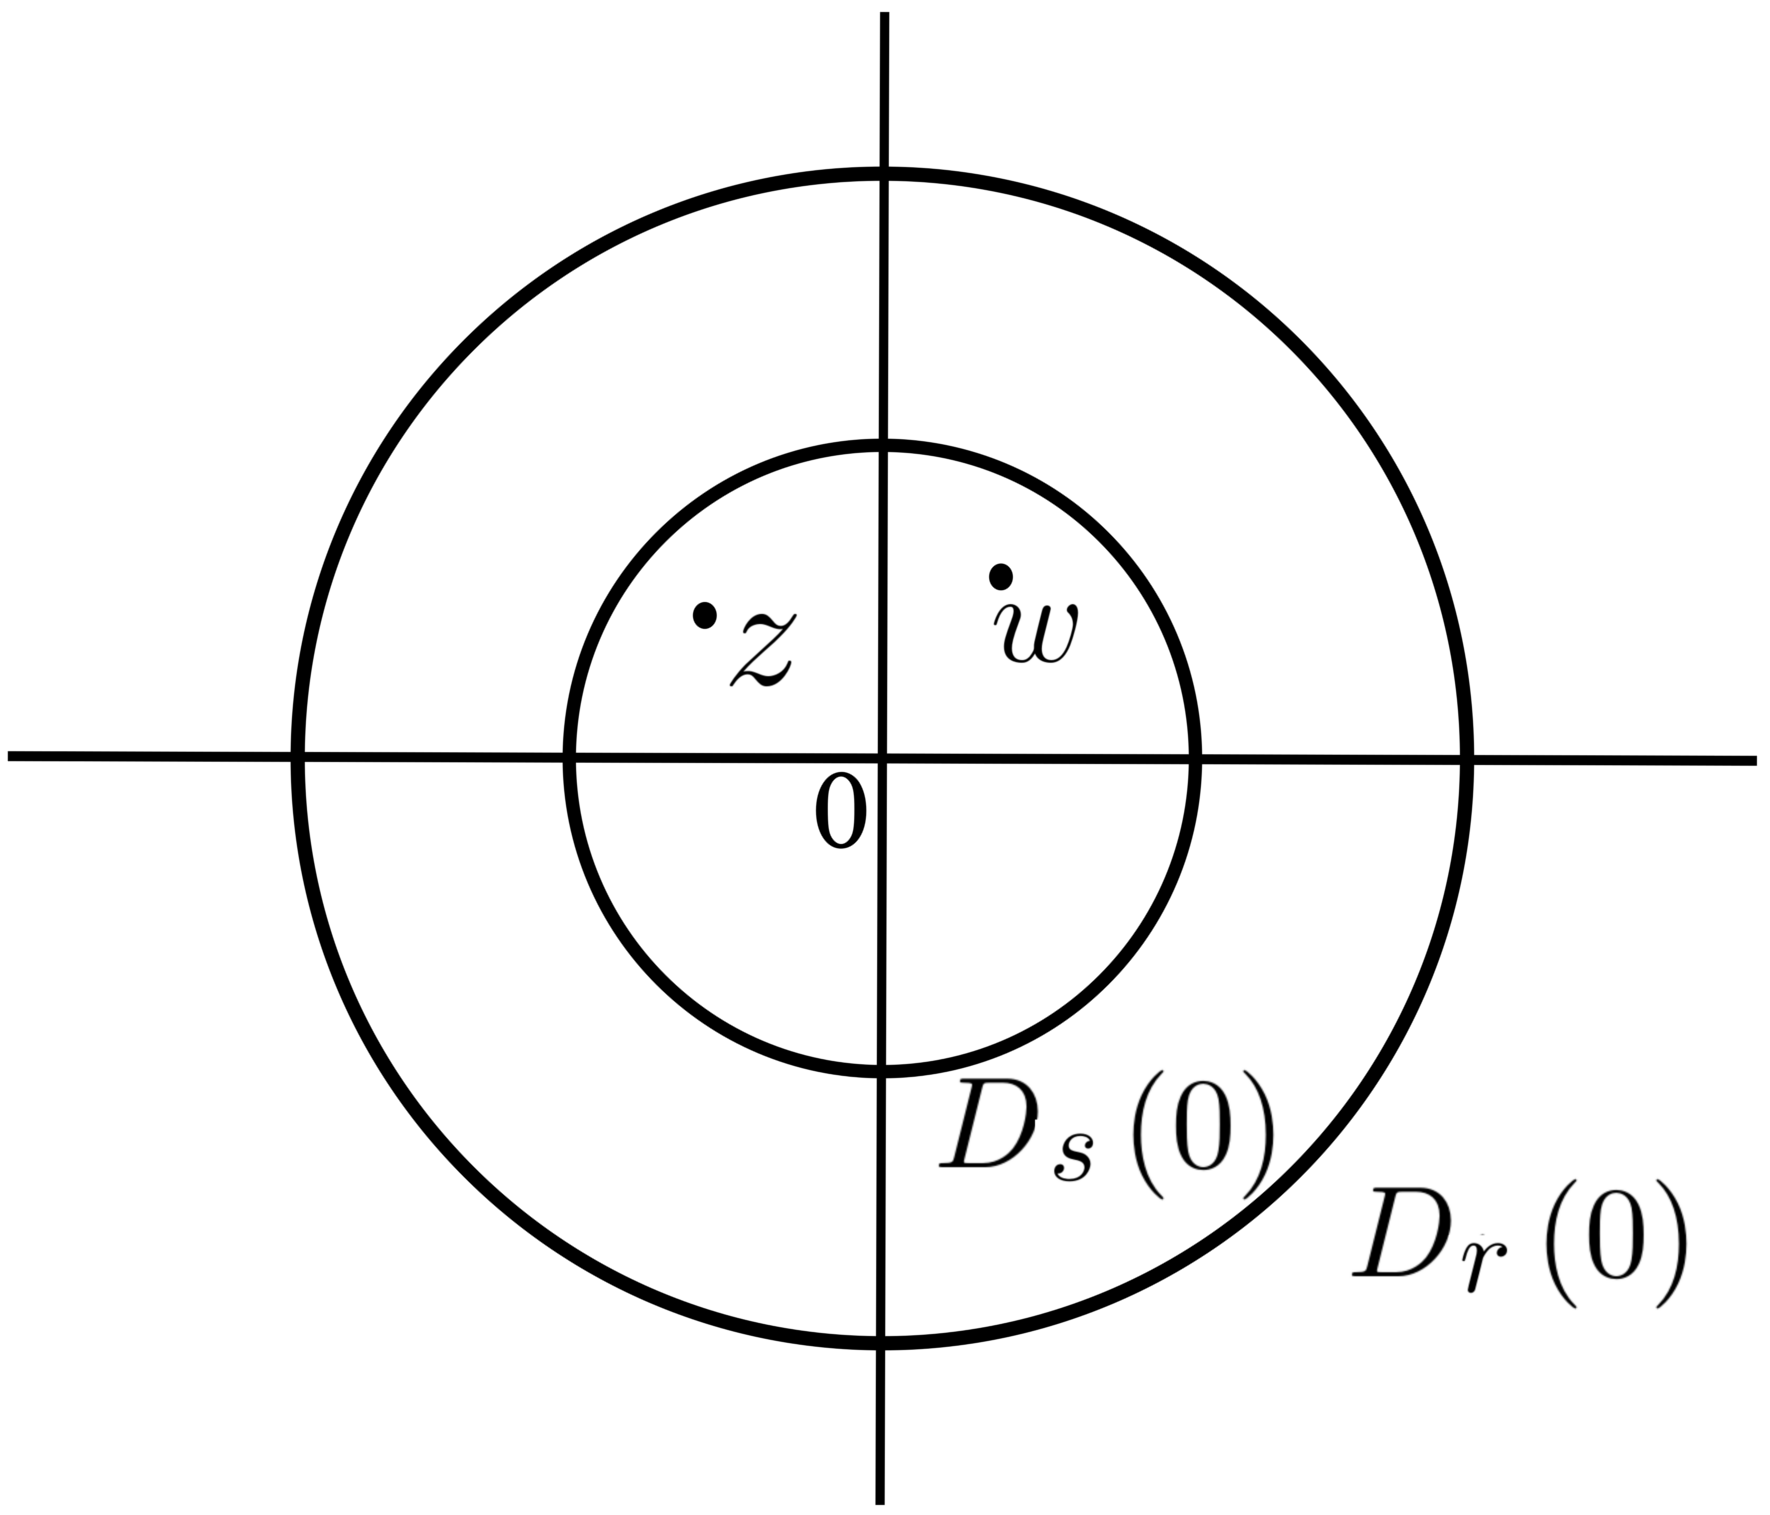
\includegraphics[width=0.3\textwidth]{4.png}
\end{center}


É imediato verificar que

\bigskip\ \ \ \ \ $%
%TCIMACRO{\QDOVERD{.}{.}{z^{m}-w^{m}}{z-w}}%
%BeginExpansion
\genfrac{.}{.}{}{0}{z^{m}-w^{m}}{z-w}%
%EndExpansion
-mw^{m-1}=\left\{
\begin{array}
[c]{c}%
0,\text{ \ se }m=1\text{ \ \ \ \ \ \ \ \ \ \ \ \ \ \ \ \ \ \ \ \ \ \ \ \ \ \ }%
\\
\\
(  z-w)  \underset{}{\overset{m-1}{\underset{k=1}{\sum}}}%
kw^{k-1}z^{m-k-1},\text{ se }m\geq2
\end{array}
\right.  $

(De fato, no caso $m\geq2,$ basta desenvolver o 2%
%TCIMACRO{\U{ba} }%
%BeginExpansion
${{}^o}$
%EndExpansion
membro obtendo

$\underset{k=1}{\overset{m-1}{\sum}}z^{m-k}w^{k-1}-(  m-1)
w^{m-1}.$ Nesta expressão basta agora somar e

subtrair $w^{m-1},$ o resultado é precisamente o 1%
%TCIMACRO{\U{ba} }%
%BeginExpansion
${{}^o}$
%EndExpansion
membro)

em consequência, se $z\neq w$ e $\left\vert z\right\vert <s,$ para todo
$m\geq2$ \ temos:

\bigskip

$\ \ \ \ \ \ \ \ \ \ \ \ \ \ \ \ \ \ \left\vert
%TCIMACRO{\QDOVERD{.}{.}{z^{m}-w^{m}}{z-w}}%
%BeginExpansion
\genfrac{.}{.}{}{0}{z^{m}-w^{m}}{z-w}%
%EndExpansion
-mw^{m-1}\right\vert =\left\vert z-w\right\vert \left\vert \underset
{k=1}{\overset{m-1}{\sum}}kw^{k-1}z^{m-k-1}\right\vert \leq$

$\ \ \ \ \ \ \ \ \ \ \ \ \ \ \ \ \ \ \ \left\vert z-w\right\vert \cdot
\overset{m-1}{\underset{k=1}{\sum}}k\left\vert w\right\vert ^{k-1}%
\cdot\left\vert z\right\vert ^{m-k-1}<\left\vert z-w\right\vert \underset
{k=1}{\overset{m-1}{\sum}}ks^{m-2}=$

$\ \ \ \ \ \ \ \ \ \ \ \ \ \ \ \ \ \ \left\vert z-w\right\vert
%TCIMACRO{\QDOVERD{.}{.}{m(  m-1)  }{2}}%
%BeginExpansion
\genfrac{.}{.}{}{0}{m(  m-1)  }{2}%
%EndExpansion
s^{m-2}<\left\vert z-w\right\vert m^{2}s^{m-2},$

e então por $(  4.6.1)  $ temos

\bigskip

$(  4.6.2)  $ \ \ $\left\vert
%TCIMACRO{\QDOVERD{.}{.}{f(  z)  -f(  w)  }{z-w}}%
%BeginExpansion
\genfrac{.}{.}{}{0}{f(  z)  -f(  w)  }{z-w}%
%EndExpansion
-g(  w)  \right\vert \leq\left\vert z-w\right\vert \underset
{m\geq2}{\sum}\left\vert c_{m}\right\vert m^{2}s^{m-2}$ \ \ $\forall$ $z\in
D_{s}(  0)  ,$

$z\neq w$

Vamos mostrar, com um raciocínio análogo ao Lema 3.11 que a série

\ \ \ \ \ \ \ \ \ \ \ \ \ \ \ \ \ \ \ \ \ \ \ \ \ \ $\underset{m\geq2}{\sum
}\left\vert c_{m}\right\vert m^{2}s^{m-2}$

é convergente. De fato, como $\sum c_{m}z^{m}$ converge em $D_{r}(
0)  $ (para $f(  z)  $), o

raio de convergência $\rho$ desta série é $\geq r$ (ver Obs
$\left[  2\right]  $ logo após a \ Def.

4.1) e então escolhendo um número real $t$ \ tal que $s<t<r,$ \ resulta

$t<\rho$ \ e \ em consequência a série $\sum\left\vert c_{m}%
\right\vert t^{m}$ é convergente, isto é

\ \ \ \ \ \ \ \ \ \ \ \ \ \ \ \ \ \ \ \ \ \ \ \ \ 

\ \ \ \ \ \ \ \ \ \ \ \ \ \ \ \ \ \ \ \ \ \ \ \ \ \ \ $M=\sum\left\vert
c_{m}\right\vert t^{m}<+\infty$

donde $\left\vert c_{m}\right\vert t^{m}\leq M$ para cada $m\in%
%TCIMACRO{\U{2115} }%
%BeginExpansion
\mathbb{N}
%EndExpansion
,$ o que implica

\bigskip

$m^{2}\left\vert c_{m}\right\vert s^{m-2}=%
%TCIMACRO{\QDOVERD{.}{.}{1}{t^{2}}}%
%BeginExpansion
\genfrac{.}{.}{}{0}{1}{t^{2}}%
%EndExpansion
(  \left\vert c_{m}\right\vert t^{m})  m^{2}(
%TCIMACRO{\QDOVERD{.}{.}{s}{t}}%
%BeginExpansion
\genfrac{.}{.}{}{0}{s}{t}%
%EndExpansion
)  ^{m-2}\leq%
%TCIMACRO{\QDOVERD{.}{.}{1}{t^{2}}}%
%BeginExpansion
\genfrac{.}{.}{}{0}{1}{t^{2}}%
%EndExpansion
Mm^{2}(
%TCIMACRO{\QDOVERD{.}{.}{s}{t}}%
%BeginExpansion
\genfrac{.}{.}{}{0}{s}{t}%
%EndExpansion
)  ^{m-2},$ \ $\forall$ \ $m\geq2$

e portanto

\ \ \ \ \ \ \ \ \ \ \ \ \ \ \ $L:=\underset{m\geq2}{\sum}m^{2}\left\vert
c_{m}\right\vert s^{m-2}\leq%
%TCIMACRO{\QDOVERD{.}{.}{1}{t^{2}}}%
%BeginExpansion
\genfrac{.}{.}{}{0}{1}{t^{2}}%
%EndExpansion
M\underset{m\geq2}{\sum}m^{2}(
%TCIMACRO{\QDOVERD{.}{.}{s}{t}}%
%BeginExpansion
\genfrac{.}{.}{}{0}{s}{t}%
%EndExpansion
)  ^{m-2}<+\infty,$

pois pelo teste da razão temos

\bigskip

$\underset{m\rightarrow\infty}{\limsup}%
%TCIMACRO{\QDOVERD{.}{.}{(  m+1)  ^{2}(  \frac{s}{t})
%^{m-1}}{m^{2}(  \frac{s}{t})  ^{m-2}}}%
%BeginExpansion
\genfrac{.}{.}{}{0}{(  m+1)  ^{2}(  \frac{s}{t})
^{m-1}}{m^{2}(  \frac{s}{t})  ^{m-2}}%
%EndExpansion
=\underset{m\rightarrow\infty}{\lim}(
%TCIMACRO{\QDOVERD{.}{.}{m+1}{m}}%
%BeginExpansion
\genfrac{.}{.}{}{0}{m+1}{m}%
%EndExpansion
)  ^{2}(
%TCIMACRO{\QDOVERD{.}{.}{s}{t}}%
%BeginExpansion
\genfrac{.}{.}{}{0}{s}{t}%
%EndExpansion
)  =%
%TCIMACRO{\QDOVERD{.}{.}{s}{t}}%
%BeginExpansion
\genfrac{.}{.}{}{0}{s}{t}%
%EndExpansion
<1.$

\bigskip

Por $(  4.6.2)  $ podemos escrever então:

\bigskip

$\ \ \ \ \ \ \left\vert
%TCIMACRO{\QDOVERD{.}{.}{f(  z)  -f(  w)  }{z-w}}%
%BeginExpansion
\genfrac{.}{.}{}{0}{f(  z)  -f(  w)  }{z-w}%
%EndExpansion
-g(  w)  \right\vert \leq\left\vert z-w\right\vert L$ \ \ $\forall$
\ $z\in D_{s}(  0)  ,$ \ $z\neq w$

\bigskip

o que prova que $\underset{z\rightarrow w}{\lim}%
%TCIMACRO{\QDOVERD{.}{.}{f(  z)  -f(  w)  }{z-w}}%
%BeginExpansion
\genfrac{.}{.}{}{0}{f(  z)  -f(  w)  }{z-w}%
%EndExpansion
-g(  w)  =0,$ isto é

$\bigskip$

$f^{\prime}(  w)  =\underset{z\rightarrow w}{\lim}%
%TCIMACRO{\QDOVERD{.}{.}{f(  z)  -f(  w)  }{z-w}}%
%BeginExpansion
\genfrac{.}{.}{}{0}{f(  z)  -f(  w)  }{z-w}%
%EndExpansion
=g(  w)  ,$ o que pela definição de $g$ \ implica

\ \ \ \ \ \ \ \ \ \ \ \ 

\ \ \ \ \ \ \ \ \ \ \ \ \ \ \ \ \ \ \ \ \ \ \ \ \ $f^{\prime}(  z)
=\sum mc_{m}z^{m-1}$ \ $\forall$ \ $z\in D_{r}(  0)  ,$

\bigskip

portanto $f\in\mathcal{H}(  \Omega)  $ \ e \ $f^{\prime}%
\in\mathcal{A}(  \Omega)  .$ \ $\square$

\bigskip

\textbf{Corolário 4.7 \ }\textit{Seja }$\sum c_{m}(  z-\zeta)
^{m}$ \textit{uma série de} \textit{potências em volta}

\textit{de }$\zeta$ \textit{de raio de convergência }$\rho>0$ \textit{e
seja }$f$ \textit{sua soma, isto é}

\bigskip

$(  4.7.1)  $ \ \ \ \ \ \ $f(  z)  =\underset{m\geq
0}{\sum}c_{m}(  z-\zeta)  ^{m}$ \ \ $\forall$ \ $z\in D_{\rho
}(  \zeta)  $

\textit{Então \ }$f\in\mathcal{H}(  D_{\rho}(  \zeta)
)  .$

\bigskip

\textbf{Prova \ }Seja $g(  z)  =\underset{m\geq1}{\sum}%
mc_{m}(  z-\zeta)  ^{m-1}$ \ $\forall$ \ $z\in D_{\rho}(
\zeta)  ,$ então basta observar

que na prova feita no Teor. 4.6 de que para cada $w\in D_{\rho}(
\zeta)  $ se tem

$\underset{z\rightarrow w}{\lim}%
%TCIMACRO{\QDOVERD{.}{.}{f(  z)  -f(  w)  }{z-w}}%
%BeginExpansion
\genfrac{.}{.}{}{0}{f(  z)  -f(  w)  }{z-w}%
%EndExpansion
=g(  w)  ,$ não foi usado o fato de $f$ \ ser analítica, apenas

foi usada $(  4.7.1)  .$ \ $\square$

\bigskip

Dada uma função $f\in\mathcal{H}(  \Omega)  $ está
associada a ela uma função $f^{\prime}:\Omega\rightarrow%
%TCIMACRO{\U{2102} }%
%BeginExpansion
\mathbb{C}
%EndExpansion
$

chamada \ \textit{derivada primeira de }$f$ (ou simplesmente derivada de $f$). Por

uniformidade de notação indicaremos $f$ por $f^{(  0)  }$ e
$f^{\prime}$ por $f^{(  1)  };$ com estas

notações definimos para cada $k\in%
%TCIMACRO{\U{2115} }%
%BeginExpansion
\mathbb{N}
%EndExpansion
$ uma aplicação $f^{(  k+1)  }:\Omega\rightarrow%
%TCIMACRO{\U{2102} }%
%BeginExpansion
\mathbb{C}
%EndExpansion
$ por

\ \ \ \ \ \ \ \ \ \ \ \ \ \ \ \ $f^{(  k+1)  }=(  f^{(
k)  })  ^{\prime}=(  f^{(  k)  })  ^{(
1)  }$

que é chamada \textit{derivada }$(  k+1)  $-\textit{ésima
}de $f$ em $\Omega$ (ou também \textit{derivada}

\textit{de ordem }$k+1$ \textit{de }$f$ \textit{em }$\Omega$) isto é

\ \ \ \ \ \ \ \ \ \ \ \ \ \ \ $f^{(  2)  }=(  f^{\prime
})  ^{\prime}=(  f^{(  1)  })  ^{(  1)
};$ \ \ \ \ \ $f^{(  3)  }=(  f^{(  2)  })
^{\prime},$ \ \ \ \ \ \ etc.

\bigskip

Observemos que em princípio $f^{(  k)  }$\bigskip\ poderia
não ser holomorfa em $\Omega$ e

portanto $(  f^{(  k)  })  ^{\prime}=f^{(
k+1)  }$ não existir, porém não é o que acontece para o

subconjunto $\mathcal{A}(  \Omega)  $ de $\mathcal{H}(
\Omega)  ,$ como resulta de modo quase evidente do

Teor. 4.6 e fica estabelecido de modo preciso no resultado seguinte:

\bigskip

\textbf{Corolário 4.8 \ }\textit{Seja }$f\in\mathcal{A}(
\Omega)  .$\textit{\ Então, para cada }$k\in%
%TCIMACRO{\U{2115} }%
%BeginExpansion
\mathbb{N}
%EndExpansion
$ \textit{existe }

$f^{(  k)  }:\Omega\rightarrow%
%TCIMACRO{\U{2102} }%
%BeginExpansion
\mathbb{C}
%EndExpansion
$ (isto é, $f$ possui derivadas de todas as ordens em $\Omega)$ \textit{e}

\textit{\ }$f^{(  k)  }\in\mathcal{A}(  \Omega)  .$
\textit{De modo mais preciso, se }$D_{r}(  \zeta)  \subset\Omega$
\textit{e}

\bigskip

$(  4.8.1)  $ \ \ \ \ \ \ $f(  z)  =\underset{m\geq
0}{\sum}c_{m}(  z-\zeta)  ^{m}$ \ \ \textit{para cada \ }$z\in
D_{r}(  \zeta)  $

\textit{então, para cada }$k\in%
%TCIMACRO{\U{2115} }%
%BeginExpansion
\mathbb{N}
%EndExpansion
,$ $\ k\geq1$ \textit{temos:}

\bigskip

$(  4.8.2)  $ \ \ \ \ \ \ \ $f^{(  k)  }(
z)  =\underset{m\geq k}{\sum}m(  m-1)  $ $\ldots$ $(
m-k+1)  c_{m}(  z-\zeta)  ^{m-k}$

\textit{para todo }$z\in D_{r}(  \zeta)  .$

\bigskip

\textbf{Prova \ }A prova é por indução porém é tão
simples que vamos nos

limitar a mostrar informalmente este processo indutivo. Dada $f\in
\mathcal{A}(  \Omega)  ,$

pelo Teor. 4.6, existe $f^{\prime}=f^{(  1)  }:\Omega\rightarrow%
%TCIMACRO{\U{2102} }%
%BeginExpansion
\mathbb{C}
%EndExpansion
$ e $f^{(  1)  }\in\mathcal{A}(  \Omega)  $ e portanto podemos

aplicar o Teor. 4.6 a $f^{(  1)  }.$ Resulta que existe $f^{(
2)  }:\Omega\rightarrow%
%TCIMACRO{\U{2102} }%
%BeginExpansion
\mathbb{C}
%EndExpansion
$ e que $f^{(  2)  }\in$

$\mathcal{A}(  \Omega)  ,$ \ etc. A prova de $(  4.8.2)
$ também é feita por indução sobre $k$. A

expressão de $f^{\prime}=f^{(  1)  }$ em \ $D_{r}(
\zeta)  $ dada pelo Teor. 4.6 prova que $(  4.8.2)  $

é verdadeira \ para $k=1.$ Supondo $(  4.8.2)  $ verdadeira,
devemos provar

\bigskip

$(  4.8.3)  $ \ \ \ $f^{(  k+1)  }(  z)
=\underset{m\geq k+1}{\sum}m(  m-1)  $ $\ldots$ $(
m-k+1)  (  m-k)  (  z-\zeta)  ^{m-(
k+1)  } $

$\ \ \ \ \ \ \ \ \ \ \ \ \ \forall$ \ $z\in D_{r}(  \zeta)  $

o que é imediato pois como $f^{(  k)  }\in\mathcal{A}(
\Omega)  $ e $f^{(  k)  }$ é representada em
$D_{r}(  \zeta)  $

pelo segundo membro de $(  4.8.2)  $ (hipótese de
indução), aplicando o Teor.

4.6 a $f^{(  k)  }$ obtemos precisamente $(  4.8.3)  .$
\ $\square$

\bigskip

\textbf{Corolário 4.9 \ }\textit{Seja }$f\in\mathcal{A}(
\Omega)  .$ \textit{Então, para cada }$\zeta\in\Omega$ \textit{e
para cada }$r>0$

\textit{tal que }$D_{r}(  \zeta)  \subset\Omega$ \textit{temos:}

\ \ \ \ \ \ \ \ \ \ \ \ \ \ \ \ \ \ \ \ \ \ \ \ $f(  z)
=\underset{m\geq0}{\sum}%
%TCIMACRO{\QDOVERD{.}{.}{1}{m!}}%
%BeginExpansion
\genfrac{.}{.}{}{0}{1}{m!}%
%EndExpansion
f^{(  m)  }(  \zeta)  (  z-\zeta)  ^{m},$
\ \textit{para cada \ }$z\in D_{r}(  \zeta)  .$

\bigskip

\textbf{Prova \ }Fixados $\zeta\in\Omega$ e $r>0$ tal que $D_{r}(
\zeta)  \subset\Omega,$ pela Def. 4.1 existe uma

série de potências $\sum c_{m}(  z-\zeta)  ^{m}$ que
representa $f$ em $D_{r}(  \zeta)  $, isto é

\bigskip

$(  4.9.1)  $ \ \ \ \ \ \ \ \ \ \ \ \ \ $f(  z)
=\underset{m\geq0}{\sum}c_{m}(  z-\zeta)  ^{m}$ \ \ $\forall$
\ $z\in D_{r}(  \zeta)  $

e em consequência, pelo Corol. 4.8, para cada $k\in%
%TCIMACRO{\U{2115} }%
%BeginExpansion
\mathbb{N}
%EndExpansion
^{\ast}:$

\bigskip

$(  4.9.2)  $\ $\ f^{(  k)  }(  z)  =\sum
m(  m-1)  \ldots(  m-k+1)  c_{m}(  z-\zeta)
^{m-k},$ \ $\forall$ \ $z\in D_{r}(  \zeta)  $

\bigskip

Fazendo $z=\zeta$ em $(  4.9.1)  $ obtemos $c_{0}=f(
\zeta)  =%
%TCIMACRO{\QDOVERD{.}{.}{1}{0!}}%
%BeginExpansion
\genfrac{.}{.}{}{0}{1}{0!}%
%EndExpansion
f^{(  0)  }(  \zeta)  .$

Para $k\in%
%TCIMACRO{\U{2115} }%
%BeginExpansion
\mathbb{N}
%EndExpansion
^{\ast},$ fazendo $z=\zeta$ em $(  4.9.2)  $ obtemos (lembrar que trabalhando

com séries de potências sempre é feita a convenção
$0^{0}=1$)

$f^{(  k)  }(  \zeta)  =\underset{m\geq k}{\sum}m(
m-1)  $ $\ldots(  m-k+1)  c_{m}0^{m-k}=k(  k-1)  $
$\ldots(  k-k+1)  c_{k}$

$=k!c_{k}$ o que implica $c_{k}=%
%TCIMACRO{\QDOVERD{.}{.}{1}{k!}}%
%BeginExpansion
\genfrac{.}{.}{}{0}{1}{k!}%
%EndExpansion
f^{(  k)  }(  \zeta)  .$ Provamos assim que

\bigskip


\ \ \ \ \ \ \ \ \ \ \ \ \ \ \ \ \ \ \ \ \ \ \ \ \ \ \ \ \ \ \ \ $c_{m}=%
%TCIMACRO{\QDOVERD{.}{.}{1}{m!}}%
%BeginExpansion
\genfrac{.}{.}{}{0}{1}{m!}%
%EndExpansion
f^{(  m)  }(  \zeta)  $ \ \ $\forall$ \ $m\in%
%TCIMACRO{\U{2115} }%
%BeginExpansion
\mathbb{N}
%EndExpansion
$

\bigskip


o que substituído em $(  4.9.1)  $ demonstra o resultado.
\ $\square$

\bigskip

\textbf{Observação \ }O Corol. 4.9 mostra dois fatos importantes sobre
a série

de potências

\ \ \ \ \ \ \ \ \ \ \ \ \ \ \ \ \ \ \ \ \ \ \ \ \ \ $\sum c_{m}$ $(
z-\zeta)  ^{m}$


\bigskip


que, com a notação da Def. 4.1, representa $f$ em $D_{r}(
\zeta)  :$

\bigskip

$\left[  1\right]  $ \ Esta série é única já que $c_{m}=%
%TCIMACRO{\QDOVERD{.}{.}{1}{m!}}%
%BeginExpansion
\genfrac{.}{.}{}{0}{1}{m!}%
%EndExpansion
f^{(  m)  }(  \zeta)  $ \ $\forall$ \ $m\in%
%TCIMACRO{\U{2115} }%
%BeginExpansion
\mathbb{N}
%EndExpansion
$

\bigskip

$\left[  2\right]  $ \ Esta série depende apenas do ponto $\zeta$ e
não do $r>0$ tal que

$D_{r}(  \zeta)  \subset\Omega$ (como aparentemente deveria ocorrer
de acordo com a

Def. 4.1).

\bigskip

\textbf{Definição 4.10 \ }Sejam $f\in\mathcal{A}(  \Omega)
,$ $\zeta\in\Omega$ e $r>0$ tal que $D_{r}(  \zeta)  \subset
\Omega.$ A

série de potências em volta de $\zeta:$

\ \ \ \ \ \ \ \ \ \ \ \ \ \ \ \ \ \ \ \ $\underset{m\geq0}{\sum}%
%TCIMACRO{\QDOVERD{.}{.}{1}{m!}}%
%BeginExpansion
\genfrac{.}{.}{}{0}{1}{m!}%
%EndExpansion
f^{(  m)  }(  \zeta)  (  z-\zeta)  ^{m} $

(única que converge pontualmente para $f$ em $D_{r}(  \zeta)  )
$ é chamada \textit{série }

\textit{de Taylor de }$f$ \textit{no ponto }$\zeta.$

% IMAGEM cinco ao lado do texto:
%\begin{wrapfigure}[8]{r}{6cm}
% \centering
% \includegraphics[width=6cm]{5_novo.png}
%\end{wrapfigure}

% IMAGEM 5
\begin{center}
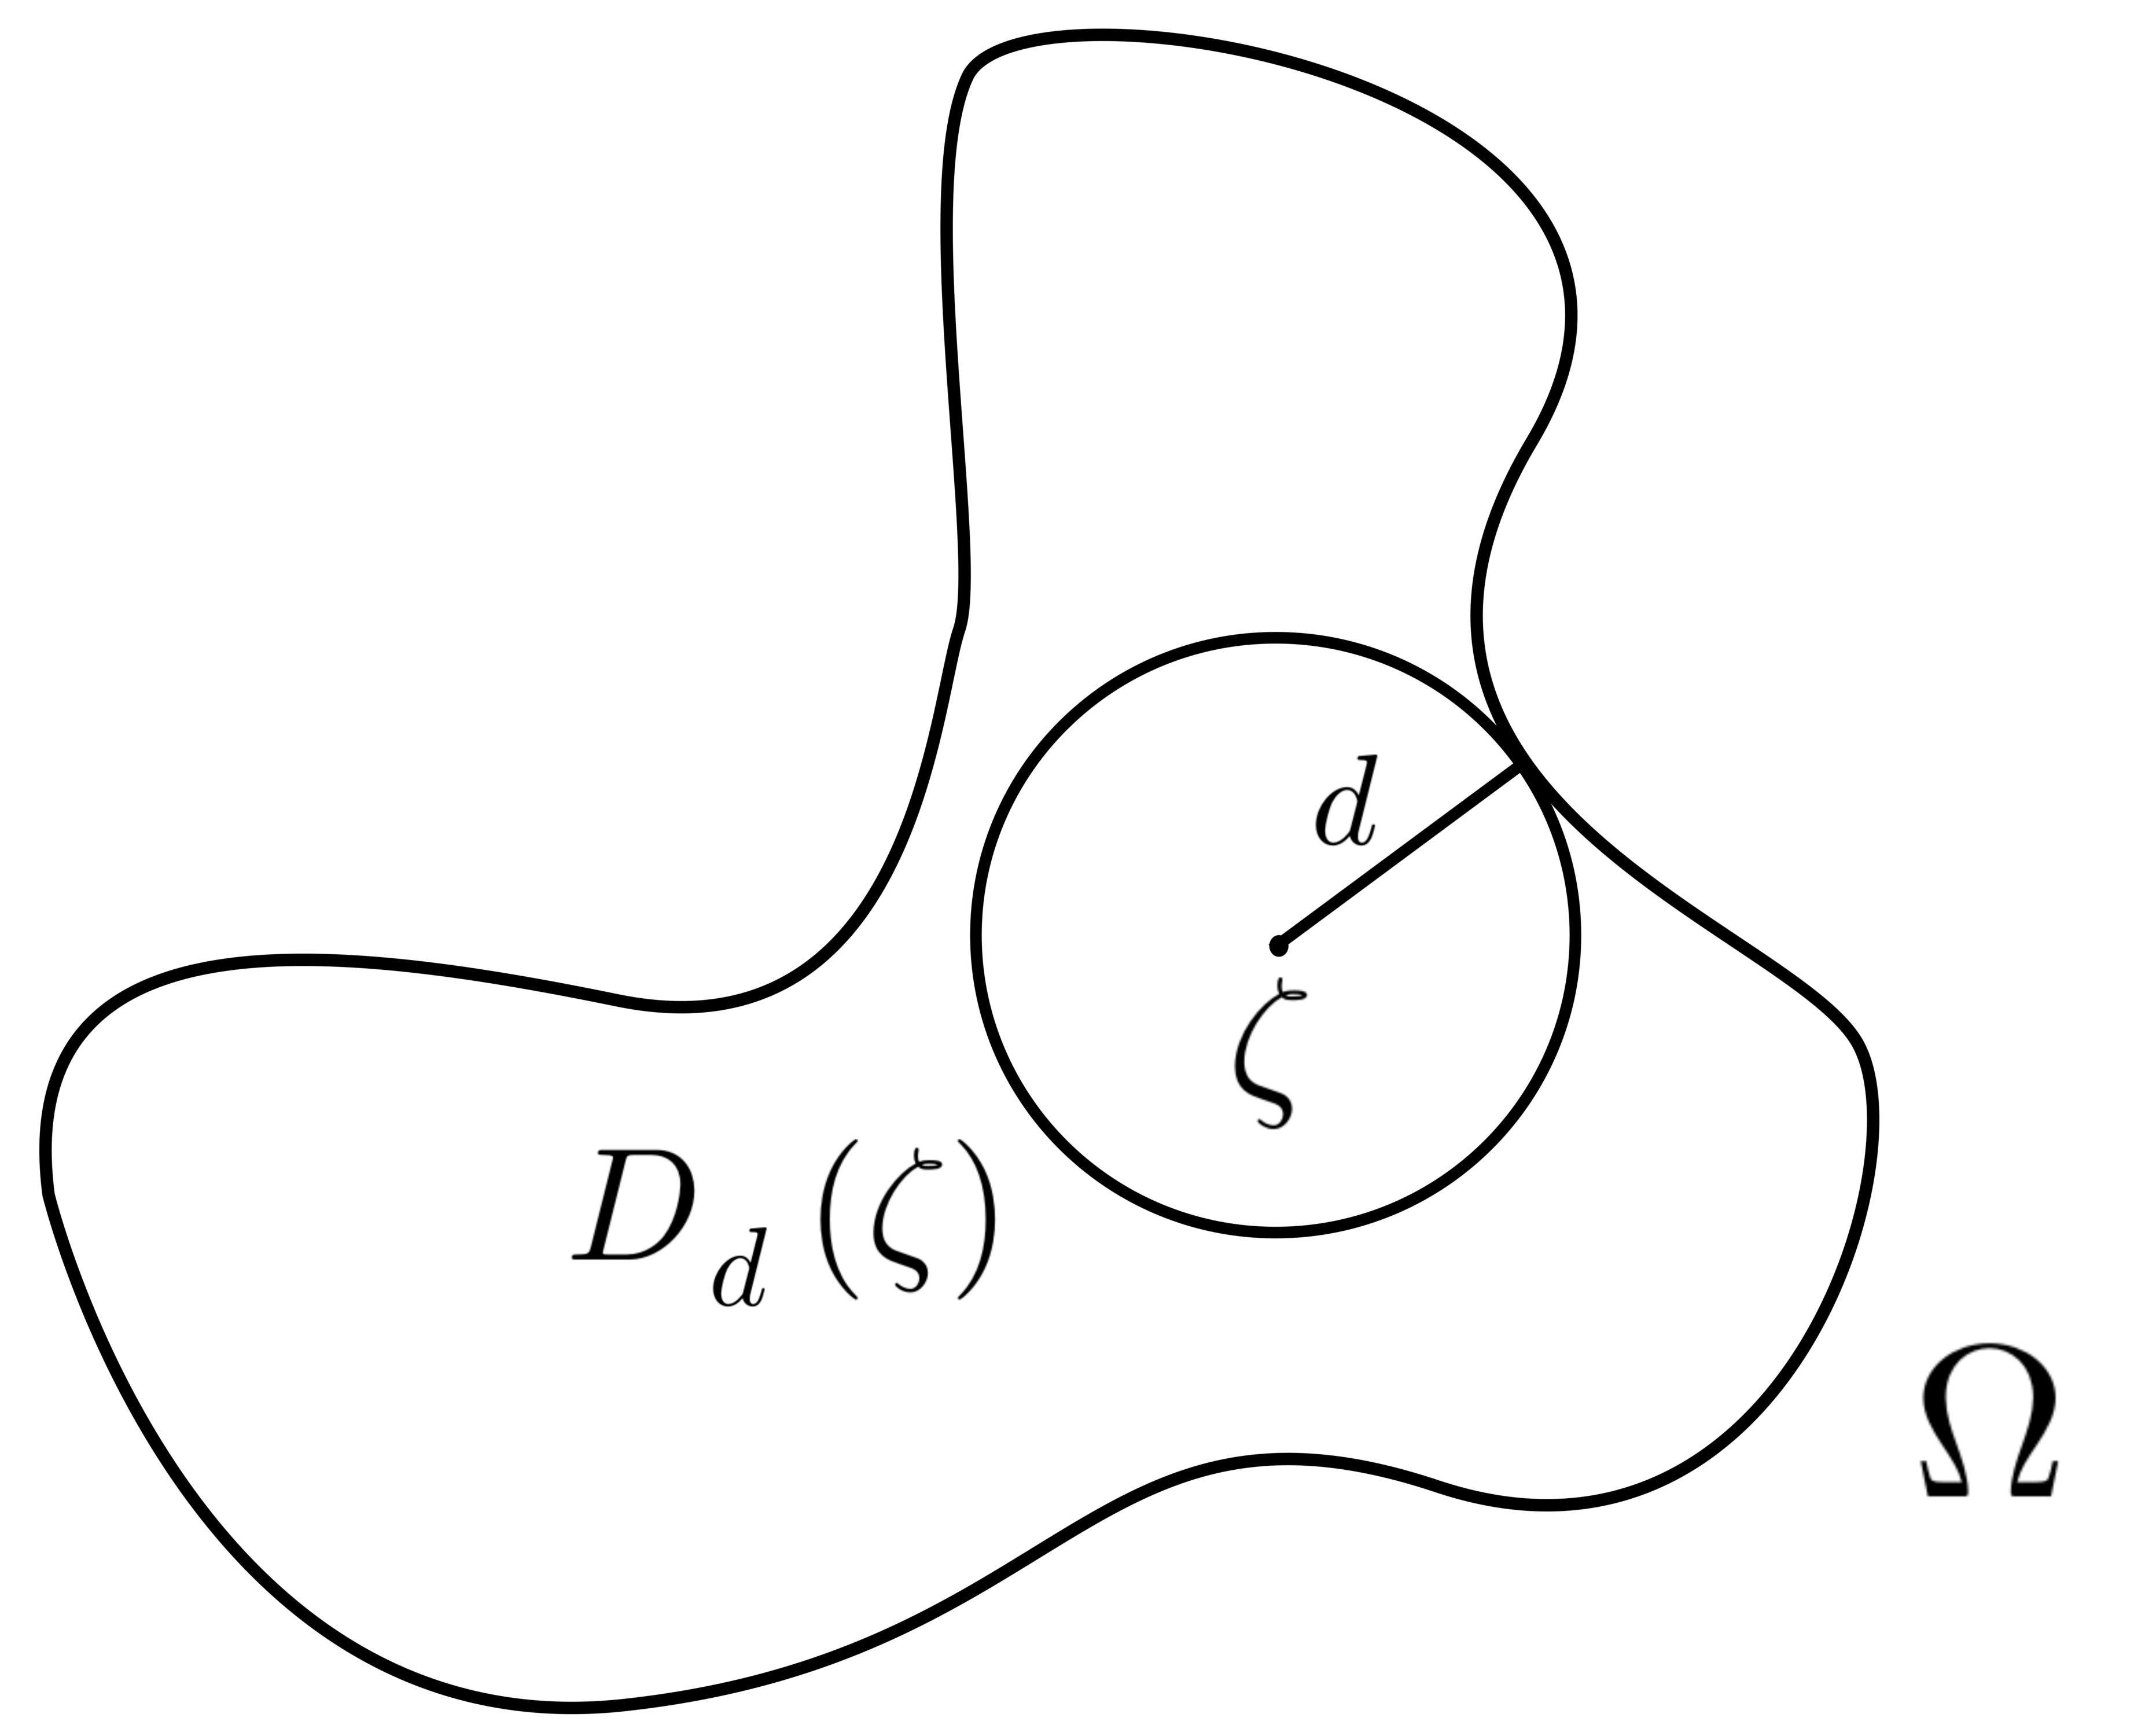
\includegraphics{5.png}
\end{center}


 \ \ \ \ \ \ \ \ \ \ \ \ \ \ \ \ \ \ \ \ \ \ \ \ \ \


A \textbf{Obs }$\left[  2\right]  $ acima pode ser enunciada de forma muito mais precisa dizendo

 que \textit{a série de Taylor de }$f$ \textit{em }$\zeta$ \textit{\ converge } \textit{pontualmente para }$f$  \textit{no maior} 
 
\textit{disco aberto de centro }$\zeta$ \textit{contido em }$\Omega,$ este é o significado do resultado
 
  seguinte:

\bigskip

%\textbf{Corolário 4.11 \ }\textit{Sejam }$f\in\mathcal{A}(\Omega) ,$ $\zeta\in \Omega$ 
%
%\ \ \ \ \ \ \ \ \ \ \ \ \ \ \ $d=dist(  \zeta,%

\textbf{Corol\'{a}rio 4.11 \ }\textit{Sejam }$f\in \mathcal{A}( \Omega
) ,$ $\zeta \in \Omega $ e \\ \ 

\ \ \ \ \ \ \ \ \ \ \ \ \ \ \ $d=dist( \zeta ,%
%TCIMACRO{\U{2102} }%
%BeginExpansion
\mathbb{C}
%EndExpansion
\backslash\Omega)  =\left\{
\begin{array}
[c]{c}%
\inf\left\{  \left\vert z-\zeta\right\vert \text{ }|\text{ }z\in%
%TCIMACRO{\U{2102} }%
%BeginExpansion
\mathbb{C}
%EndExpansion
\backslash\Omega\right\}  ,\ \text{\textit{se }}\mathit{\ }\Omega\neq%
%TCIMACRO{\U{2102}}%
%BeginExpansion
\mathbb{C}%
%EndExpansion
\\
+\infty,\text{ \ \textit{se }}\Omega=%
%TCIMACRO{\U{2102} }%
%BeginExpansion
\mathbb{C}.
%EndExpansion
\text{ \ \ \ \ \ \ \ \ \ \ \ \ \ \ \ \ \ \ \ }%
\end{array}
\right.  $

\textit{Então }

$(  4.11.1)  $ \ \ \ \ \ \ \ \ \ \ $f(  z)
=\underset{m\geq0}{\sum}%
%TCIMACRO{\QDOVERD{.}{.}{1}{m!}}%
%BeginExpansion
\genfrac{.}{.}{}{0}{1}{m!}%
%EndExpansion
f^{m}(  \zeta)  (  z-\zeta)  ^{m}$ \ \ $\forall$ \ $z\in
D_{d}(  \zeta)  $

\textit{e em consequência, o raio de convergência da série de
Taylor de }$f$ \textit{no}

\textit{ponto }$\zeta$ \textit{é }$\geq d.$

\bigskip

\textbf{Prova} \ Pelo Corol. 4.9 temos

\ \ \ \ \ \ \ \ \ \ \ \ \ \ \ \ \ \ \ \ \ \ $f(  z)  =\underset
{m\geq0}{\sum}%
%TCIMACRO{\QDOVERD{.}{.}{1}{m!}}%
%BeginExpansion
\genfrac{.}{.}{}{0}{1}{m!}%
%EndExpansion
f^{(  m)  }(  \zeta)  (  z-\zeta)  ^{m},$
\ \ $\forall$ \ $z\in D_{r}(  \zeta)  $

e para cada $r>0$ tal que $D_{r}(  \zeta)  \subset\Omega.$ Se
$\Omega=%
%TCIMACRO{\U{2102} }%
%BeginExpansion
\mathbb{C}
%EndExpansion
$ é evidente, se $\Omega\neq%
%TCIMACRO{\U{2102} }%
%BeginExpansion
\mathbb{C}
%EndExpansion
$

procedemos assim: seja $z\in D_{d}(  \zeta)  $ e suponhamos por
absurdo que $z\notin\Omega,$

então por definição de $\ "\inf$ $"$ temos $d\leq\left\vert
z-\zeta\right\vert $ o que está em contradição

com a relação $z\in D_{d}(  \zeta)  .$ A asserção
relativa ao raio de convergência da

série de Taylor segue então (4.11.1) e da \textbf{Obs }$\left[
2\right]  $ após a Def. 4.1.\ $\ \square$

\bigskip

\textbf{Observação \ }Seja $\sum c_{m}(  z-\zeta)  ^{m}$
uma série de potências em volta de $\zeta$ de

raio de convergência $\rho>0,$ então fica definida uma função

\ \ \ \ \ \ \ \ \ \ \ \ \ \ \ \ \ \ $\varphi:z\in D_{\rho}(
\zeta)  \longmapsto\underset{m\geq0}{\sum}c_{m}(  z-\zeta)
^{m}\in%
%TCIMACRO{\U{2102} }%
%BeginExpansion
\mathbb{C}
%EndExpansion
$

que é (ver \textbf{Obs }$\left[  5\right]  ,$ após a Def. 4.1)
analítica em $\zeta$ e então, uma pergunta

que surge naturalmente é a seguinte:

\ \ \ \ \ \ \ $\varphi$ é analítica em cada ponto de $D_{\rho}(
\zeta)  $? isto é: $\varphi\in\mathcal{A}(  D_{\rho}(
\zeta)  )  $?

A resposta a esta questão é afirmativa (porém não é um resultado

evidente) e, do ponto de vista da Def. 4.1, este é o exemplo mais natural

não trivial de função analítica ( os polinômios são
exemplos naturais porém

triviais de funções analíticas). A prova de que $\varphi
\in\mathcal{A}(  \Omega)  $ pode ser feita

diretamente a partir da Def. 4.1 e de alguns cálculos um tanto elaborados

com séries (ver por exemplo, [Ca, "Theorie elementaire des fonctions

analytiques d$^{\prime}$une et plusieurs variables, " Ch \textsc{I,} \S 4, n$%
%TCIMACRO{\U{ba}}%
%BeginExpansion
{{}^o}%
%EndExpansion
$ 2, Prop. 2.1, Prop.

2.2]). Nós vamos obter este resultado no \S 5 quando, usando a integração

complexa, vamos provar a recíproca do Teor. 4.6, isto é:
$\mathcal{A}(  \Omega)  =\mathcal{H}(  \Omega)  ,$

o que junto com o Corl. 4.7, implica a asserção $\varphi\in
\mathcal{A}(  D_{\rho}(  \zeta)  )  .$

\bigskip

\textbf{Teorema 4.12 \ }\textit{Sejam }$\Omega$ \textit{um aberto conexo
não vazio de }$%
%TCIMACRO{\U{2102} }%
%BeginExpansion
\mathbb{C}
%EndExpansion
$ \textit{e }$f\in\mathcal{A}(  \Omega)  .$

\textit{As condições seguintes são equivalentes:}

(i) \ \ \textit{Existe }$\zeta\in\Omega$ \textit{tal que }$f^{(
m)  }(  \zeta)  =0$ \textit{para cada }$m\in%
%TCIMACRO{\U{2115} }%
%BeginExpansion
\mathbb{N}
%EndExpansion
;$

(ii) \ \textit{Existe }$\zeta\in\Omega$ \textit{e existe }$r>0$\textit{\ tais
que }$D_{r}(  \zeta)  \subset\Omega$ \ \textit{e}

\ \ \ \ \ \ \ \ \ \ \ \ \ \ \ \ \ \ \ \ \ \ \ \ \ \ \ $f$ $|$ $D_{r}(
\zeta)  =0;$

(iii) \ \textit{Existe um subconjunto aberto não vazio }$\ W$ \textit{de
}$\Omega$ \ \textit{tal que }$f$ $|$ $W=0;$

(iv) \ $f=0$ (isto é, $f(  z)  =0$ para cada $z\in\Omega$).

\bigskip

\textbf{Prova \ }Vamos demonstrar \bigskip as seguintes implicações

\ \ \ \ \ \ \ \ \ \ \ (iv) $\implies$ (i) $\implies$ (ii) $\implies$ (iv)
\ \ \ \ e \ \ (ii) $\iff$ (iii)

A implicação (iv) $\implies$ (i) é evidente e a implicação
(i) $\implies$ (ii) resulta do

Corol. 4.9 (ou do Corol. 4.11); ambas independem da hipótese de

conexão sobre $\Omega.$ A equivalência entre (ii) e (iii) também
é trivial,

portanto só resta verificar (ii) $\implies$ (iv).

Sejam $\Omega_{1}$ $=\{z\in\Omega$ $|$ $\exists$ $\rho>0$ tal que $D_{\rho
}(  z)  \subset\Omega$ e $f$ $|$ $D_{\rho}(  z)  =0\}$ \ \ \ e

$\Omega_{2}=\Omega\backslash\Omega_{1}.$

É claro que $\Omega=\Omega_{1}\cup\Omega_{2}$ e $\Omega_{1}\cap\Omega
_{2}=\varnothing.$ A idéia da prova consiste em

verificar que $\Omega_{1}$ e $\Omega_{2}$ são abertos e que $\Omega
_{1}\neq\varnothing.$ Como $\Omega$ é conexo

resultará que $\Omega_{2}=\varnothing,$ donde $\Omega=\Omega_{1}$ e como
$f$ $|$ $\Omega_{1}=0$ obtemos

$f=f$ $|$ $\Omega=0,$ isto é (iv).

Pela definição de $\Omega_{1}$ é claro que $\Omega_{1}$ é
aberto e $f$ $|$ $\Omega_{1}=0.$ Por outro lado,

$\Omega_{1}\neq\varnothing$ pois por (ii) temos $\zeta\in\Omega_{1}$ (este
é o único lugar onde a hipótese

(ii) é utilizada). Mostremos finalmente que $\Omega_{2}$ é aberto.
Seja $z_{0}\in\Omega_{2}$ um

ponto arbitrário e mostremos que $z_{0}\in$ $\overset{\circ}{\Omega}_{2},$
isto é:

\ \ \ \ \ \ \ \ \ \ \ \ \ \ \ \ \ \ \ \ \ \ \ \ \ \ \ $\exists$ $s>0$ tal que
$D_{s}(  z_{0})  \subset\Omega_{2}$

ou, o que é equivalente:

\bigskip

$(  4.12.1)  $ \ \ \ \ \ \ \ \ \ \ \ $\exists$ \ $s>0$ tal que
$D_{s}(  z_{0})  \cap\Omega_{1}=\varnothing$

Suponhamos por absurdo que $(  4.12.1)  $ é falsa, então


$(  4.12.2)  $ \ \ \ \ \ \ \ \ $D_{s}(  z_{0})
\cap\Omega_{1}\neq\varnothing$ \ para cada $s>0$

Fixemos um $\delta>0$ tal que $D_{\delta}(  z_{0})  \subset\Omega,$
então por $(  4.12.2)  $ vem

\ \ \ \ \ \ \ \ \ \ \ \ \ \ \ \ \ \ \ \ \ \ $V=D_{\delta}(  z_{0})
\cap\Omega_{1}\neq\varnothing$

Como $f$ $|$ $\Omega_{1}=0,$ resulta $f$ $|$ $V=0$ e em consequência

\bigskip

$(  4.12.3)  $ \ \ \ \ \ \ \ \ \ \ \ $(  f\text{ }|\text{
}V)  ^{m}=f^{(  m)  }$ $|$ $V=0$ \ para cada $m\in%
%TCIMACRO{\U{2115} }%
%BeginExpansion
\mathbb{N}
%EndExpansion
$

Vamos verificar a seguir que

\bigskip

$(  4.12.4)  $ \ \ \ \ \ \ \ \ \ \ \ \ \ $f^{(  m)
}(  z_{0})  =0$ \ para cada $m\in%
%TCIMACRO{\U{2115} }%
%BeginExpansion
\mathbb{N}
%EndExpansion
$

De fato, suponhamos por absurdo que existe $m\in%
%TCIMACRO{\U{2115} }%
%BeginExpansion
\mathbb{N}
%EndExpansion
$ tal que $f^{(  m)  }(  z_{0})  \neq0,$

então existe $\sigma>0$ tal que

\ \ \ \ \ \ \ \ \ \ \ \ \ \ \ \ \ \ \ \ \ \ \ \ \ \ $0\notin D_{\sigma}(
f^{(  m)  }(  z_{0})  )  $

e como $f^{(  m)  }$ é contínua em $z_{0},$ existe
$s\in\left]  0,\delta\right[  $ tal que $f^{(  m)  }(
D_{s}(  z_{0})  )  \subset$

$D_{\sigma}(  f^{(  m)  }(  z_{0})  )  ,$ \ o
que é absurdo pois, por $(  4.12.2)  $ temos $D_{s}(
z_{0})  \cap V=$

$D_{s}(  z_{0})  \cap D_{\delta}(  z_{0})  \cap
\Omega_{1}=D_{s}(  z_{0})  \cap\Omega_{1}\neq\varnothing$ e
então para cada $w\in$

$D_{s}(  z_{0})  \cap V,$ por $(  4.12.3)  $ \ e pela
definição de $s$ teríamos:

\ \ \ \ \ \ \ \ \ \ \ \ \ \ \ \ \ \ \ \ \ \ \ \ \ \ \ \ \ \ $0=f^{(
m)  }(  w)  \in D_{\sigma}(  f^{(  m)
}(  z_{0})  )  $

o que está em contradição com a definição de $\sigma,$ o
que prova $(  4.12.4)  .$

Ora é claro que $(  4.12.4)  $ implica [mesmo raciocínio
da prova de (i) $\implies$

(ii)] que existe $\varepsilon>0$ tal que

\ \ \ \ \ \ \ \ \ \ \ \ \ \ \ \ \ \ \ \ \ \ \ \ \ \ \ \ \ \ \ \ \ $f$ $|$
$D_{\varepsilon}(  z_{0})  =0$

o que por definição implica $z_{0}\in\Omega_{1}$ e em consequência
$z_{0}\in\Omega_{1}\cap\Omega_{2}=\varnothing,$

o que é absurdo. Desta forma, provamos $(  4.12.1)  $ isto
é $\Omega_{2}$ \ é aberto. \ $\square$

\bigskip

\textbf{Observação: \ }Na verificação acima da
asserção $(  4.12.4)  $ usamos a conti-

nuidade de $f^{(  m)  },$ o que resulta dos Corol. 4.8, Teor. 4.6 e
Prop. 1.4 (1%
%TCIMACRO{\U{ba}}%
%BeginExpansion
${{}^o}$%
%EndExpansion
) que

implicam $f^{(  m)  }\in\mathcal{A}(  \Omega)
\subset\mathcal{H}(  \Omega)  \subset\mathcal{C}(
\Omega)  .$

\bigskip

\textbf{Corolário 4.13 \ }(Princípio do prolongamento analítico)
\ \textit{Sejam }$\Omega$ \textit{um }

\textit{aberto conexo não vazio de }$%
%TCIMACRO{\U{2102} }%
%BeginExpansion
\mathbb{C}
%EndExpansion
,$ $f\in\mathcal{A}(  \Omega)  $ \textit{e }$g\in\mathcal{A}(
\Omega)  .$ \textit{Se existe um sub-}

\textit{conjunto aberto não vazio }$W$ \textit{de }$\Omega$ \textit{tal
que}

\bigskip

$(  4.13.1)  $ \ \ \ \ \ \ \ \ \ \ \ \ \ \ \ \ \ $f$ $|$ $W=g$ $|$
$W,$

\textit{então \ }$f=g.$

\bigskip

\textbf{Prova \ }Como $\mathcal{A}(  \Omega)  $ é uma $%
%TCIMACRO{\U{2102} }%
%BeginExpansion
\mathbb{C}
%EndExpansion
$-álgebra, $h:=f-g\in\mathcal{A}(  \Omega)  $ e a hipótese

$(  4.13.1)  $ expressa que $h$ satisfaz a condição (iii)
do Teor. 4.12. Como $\Omega$

é conexo, $h$ satisfaz também a condição (iv) do Teor. 4.12,
logo $h=0,$

ou seja $f=g.$ \ $\square$

\bigskip

\textbf{Corolário 4.14 \ }\textit{Se }$\Omega$\textit{\ é um aberto
conexo não vazio de }$%
%TCIMACRO{\U{2102} }%
%BeginExpansion
\mathbb{C}
%EndExpansion
,$\textit{\ então }$A(  \Omega)  $

\textit{é um anel de integridade.}

\bigskip

\textbf{Prova do Corol. 4.14 usando o Teor. 4.12 \ }Sejam \ $f,g\in
\mathcal{A}(  \Omega)  $

verificando $fg=0.$ Suponhamos $f\neq0$ e mostremos que $g=0.$ Como

$f\neq0$ \ $\exists$ \ $\zeta\in\Omega$ tal que $f(  \zeta)  \neq0$
e como $f$ é contínua $\exists$ $r>0$ \ tal que

$D_{r}(  \zeta)  \subset\Omega$ \ e

$\bigskip(  4.14.1)  $ \ \ \ \ \ \ \ \ \ \ \ $f(  z)
\neq0$ \ $\forall$ \ $z\in D_{r}(  \zeta)  $

Como por hipótese $fg=0,$ em particular:

\bigskip

\ \ \ \ \ \ \ \ \ \ \ \ \ \ \ \ \ \ \ \ \ $0=(  fg)  (
z)  =f(  z)  g(  z)  $ \ \ $\forall$ \ $z\in
D_{r}(  \zeta)  $

e \ portanto por $(  4.14.1)  $ resulta $g(  z)  =0$
\ \ $\forall$ \ $z\in D_{r}(  \zeta)  $\ \ logo $g=0$ \ pelo

Teor. 4.12. $\square$

\bigskip

\textbf{Teorema 4.15 \ }(Princípio dos zeros isolados) \ \textit{Sejam
}$\Omega$ \textit{um aberto conexo}

\textit{não vazio de }$%
%TCIMACRO{\U{2102} }%
%BeginExpansion
\mathbb{C}
%EndExpansion
,$ $f\in\mathcal{A}(  \Omega)  $ \textit{e suponhamos que }%
$f\neq0.$ \textit{Então, para cada }

$\zeta\in\Omega,$ \textit{existe }$r>0$ \textit{tal que }$\ D_{r}(
\zeta)  \subset\Omega$ \textit{e }$f(  z)  \neq0$
\textit{para cada }$z\in D_{r}^{\ast}(  \zeta)  .$

\bigskip

\textbf{Prova \ }Dado $\zeta\in\Omega$ arbitrário, seja $d=dist(
\zeta,\complement\Omega)  ,$ então pelo Corol. 4.11

temos

\ \ \ \ \ \ \ \ \ \ \ \ \ \ \ $f(  z)  =\underset{m\geq0}{\sum}%
%TCIMACRO{\QDABOVE{1pt}{1}{m!}}%
%BeginExpansion
\genfrac{}{}{1pt}{0}{1}{m!}%
%EndExpansion
f^{(  m)  }(  \zeta)  (  z-\zeta)  ^{m}$
\ \ $\forall$ \ $z\in D_{d}(  \zeta)  $

Se fosse $f^{(  m)  }(  z)  =0$ para cada $m\in%
%TCIMACRO{\U{2115} }%
%BeginExpansion
\mathbb{N}
%EndExpansion
,$ como $\Omega$ é conexo resultaria (pelo

Teor. 4.12 (i) $\implies$ (iv)) $f=0$ o que é falso por hipótese. Em consequência,

o conjunto dos $m\in%
%TCIMACRO{\U{2115} }%
%BeginExpansion
\mathbb{N}
%EndExpansion
$ tais que $f^{(  m)  }(  \zeta)  \neq0$ é não
vazio e portanto possui

um mínimo, seja

$\ \ \ \ \ \ \ \ \ \ \ \ \ \ \ \ \ \ \ \ \ \ \ \ \ \ \ \nu=\min\left\{  m\in%
%TCIMACRO{\U{2115} }%
%BeginExpansion
\mathbb{N}
%EndExpansion
\text{ }|\text{ }f^{(  m)  }(  \zeta)  \neq0\right\}  .$

Podemos escrever então

\bigskip

$(  4.15.1)  $ \ \ \ \ \ \ \ \ \ $f(  z)  =(
z-\zeta)  ^{\nu}\cdot g(  z)  $ \ \ $\forall$ \ $z\in
D_{d}(  \zeta)  $

onde

\ \ \ \ \ \ \ \ \ \ \ \ \ \ \ \ \ \ \ \ \ \ $g(  z)  =\underset
{m\geq\nu}{\sum}$ $\
%TCIMACRO{\QDABOVE{1pt}{1}{m!}}%
%BeginExpansion
\genfrac{}{}{1pt}{0}{1}{m!}%
%EndExpansion
f^{(  m)  }(  \zeta)  (  z-\zeta)  ^{m-\nu}$
\ \ $\forall$ \ $z\in D_{d}(  \zeta)  $

Pelo Corol. 4.7 temos \ $g\in\mathcal{H}(  D_{d}(  \zeta)
)  $ e portanto $g\in\mathcal{C}(  D_{d}(  \zeta)
)  $ e como

por definição de $\nu$ temos

\ \ \ \ \ \ \ \ \ \ \ \ \ \ \ \ \ \ \ \ \ \ $g(  \zeta)  =%
%TCIMACRO{\QDOVERD{.}{.}{1}{\nu!}}%
%BeginExpansion
\genfrac{.}{.}{}{0}{1}{\nu!}%
%EndExpansion
f^{(  \nu)  }(  \zeta)  \neq0,$

\bigskip

existe $r>0$ tal que $D_{r}(  \zeta)  \subset D_{d}(
\zeta)  \subset\Omega$ \ e

\bigskip

$(  4.15.2)  $ \ \ \ \ \ \ \ \ \ \ \ \ \ \ $g(  z)
\neq0$ \ \ \ \ \ $\forall$ \ $z\in D_{r}(  \zeta)  $

O resultado segue então de $(  4.15.1)  $ e $(
4.15.2)  .$ \ $\square$

\bigskip

Lembremos que um subconjunto de $X$ de $%
%TCIMACRO{\U{2102} }%
%BeginExpansion
\mathbb{C}
%EndExpansion
$ é dito \textit{discreto }se $X=\varnothing$ ou

se cada ponto de $X$ é isolado, isto é, para cada $\zeta\in X$
$\ $existe $r>0$ \ tal

que $D_{r}^{\ast}(  \zeta)  \cap X=\varnothing.$

\bigskip

\textbf{Corolário 4.16 \ }\textit{Sejam }$\Omega$\textit{\ um aberto
conexo não vazio de }$%
%TCIMACRO{\U{2102} }%
%BeginExpansion
\mathbb{C}
%EndExpansion
$ \textit{e }$f\in\mathcal{A}(  \Omega)  $

\textit{tal que }$f\neq0.$ \textit{Então o conjunto}

\ \ \ \ \ \ \ \ \ \ \ \ \ \ \ \ \ \ \ \ \ \ \ $Z(  f)  :=\left\{
z\in\Omega\text{ }|\text{ }f(  z)  =0\right\}  $

\textit{é um conjunto discreto e fechado em }$\Omega.$

\bigskip

\textbf{Prova} \ Se $Z(  f)  =\varnothing$ o resultado é
óbvio. Se $Z(  f)  \neq\varnothing,$ seja $\zeta\in Z(
f)  ,$

então pelo Teor. 4.15 (mais precisamente por $(  4.15.1)  $ e
$(  4.15.2)  $)$,$ existe

$r>0,$ existe $\nu\in%
%TCIMACRO{\U{2115} }%
%BeginExpansion
\mathbb{N}
%EndExpansion
$ e existe $g\in\mathcal{H}(  D_{r}(  \zeta)  )  $ tais
que $D_{r}(  \zeta)  \subset\Omega,$ $\ g(  z)  \neq0$

para cada $\ z\in D_{r}(  \zeta)  $ \ e

\ \ \ \ \ \ \ \ \ $f(  z)  =(  z-\zeta)  ^{\nu}\cdot
g(  z)  ,$ para cada $z\in D_{r}(  \zeta)  .$

Em consequência temos

\ \ \ \ \ \ \ \ \ $f(  z)  =(  z-\zeta)  ^{\nu}g(
z)  \neq0$ \ para cada \ $z\in D_{r}^{\ast}(  \zeta)  ,$ \ 

o que mostra que $Z(  f)  $ é discreto. O conjunto $Z(
f)  $ é fechado em $\Omega$ pela

continuidade de $f.$ (ver exerc.4.9 (c)). \ $\square$

\bigskip

Sejam $\Omega$ um aberto conexo não vazio de $%
%TCIMACRO{\U{2102} }%
%BeginExpansion
\mathbb{C}
%EndExpansion
$, $\ f\in\mathcal{A}(  \Omega)  ,$ $f\neq0$ e $\ \zeta\in\Omega.$

Na prova do Teor. 4.15 vimos que existem $r>0,$ $\nu\in%
%TCIMACRO{\U{2115} }%
%BeginExpansion
\mathbb{N}
%EndExpansion
$ e $g\in\mathcal{H}(  D_{r}(  \zeta)  )  $

tais que $D_{r}(  \zeta)  \subset\Omega,$ $g(  z)
\neq0$ para cada $z\in D_{r}(  \zeta)  $ \ e

\bigskip

\ \ \ \ \ \ \ \ \ \ \ \ \ \ \ \ \ \ \ \ \ \ \ \ \ \ \ \ $f(  z)
=(  z-\zeta)  ^{\nu}.g(  z)  $ \ \ $\forall$ \ $z\in
D_{r}(  \zeta)  $

\bigskip

como resulta imediatamente de $(  4.15.1)  $ e $(
4.15.2)  .$ Se $\nu=0$ tem-se

$f(  \zeta)  =g(  \zeta)  \neq0.$ Com esta terminologia
introduzimos o conceito funda-

mental de multiplicidade (ou ordem) de um zero:

\bigskip

\textbf{Definição 4.17 \ }Com as notações acima, se $\nu\geq1$
diz-se que $\zeta$ é um

\textit{zero de} $f$ \textit{de multiplicidade (ou ordem) }$\nu$ (ou que $\nu$
é a multiplicidade do

zero que $f$ tem em $\zeta$).

\bigskip

O resultado abaixo dá uma informação mais precisa a respeito de
$Z(  f)  $:

\bigskip

\textbf{Proposição 4.18 \ }\textit{Sejam }$\Omega$\textit{\ um aberto
de }$%
%TCIMACRO{\U{2102} }%
%BeginExpansion
\mathbb{C}
%EndExpansion
,$ $f\in\mathcal{H}(  \Omega)  $ \textit{tal que }$f\neq0$
\textit{e}

\textit{suponha que }$Z(  f)  $\textit{\ é um conjunto
infinito, então:}

(a) \ $Z(  f)  $ \textit{é enumerável,}

(b) \ $Z(  f)  $ \textit{não tem ponto de acumulação em
}$\Omega$.

\bigskip

\textbf{Prova \ }(a) \ De fato, seja $(  K_{n})  _{n\geq1}$ uma
sequência exaustiva de compactos

para $\Omega$ então é claro que $Z(  f)  \cap K_{n}$ é
finito para cada $n\geq1$ (ver \cite{R1}, Teor.

2.37]) donde resulta

\ \ \ \ \ \ \ \ \ \ \ \ \ \ \ \ \ \ \ \ \ \ $\underset{n\geq1}{\bigcup}(
Z(  f)  \cap K_{n})  =Z(  f)  \cap\underset
{n\geq1}{\bigcup}K_{n}=Z(  f)  $

\bigskip

o que prova a nossa afirmação pois

\ \ \ \ \ \ \ \ \ \ \ \ \ \ \ \ \ \ \ \ $Card(  Z(  f)
)  =Card(  \underset{n\geq1}{\bigcup}(  Z(  f)
\cap K_{n})  )  \leq Card(
%TCIMACRO{\U{2115} }%
%BeginExpansion
\mathbb{N}
%EndExpansion
)  .$

(b) \ Suponha por absurdo que $p\in\Omega$ é um ponto de
acumulação de $Z(  f)  $

então existe uma sequência $(  a_{m})  _{m\geq1}$ em
$Z(  f)  $ tal que $a_{m}\rightarrow p$ se $m\rightarrow\infty$ o

que implica pela continuidade de $f$ que $f(  a_{m})  \rightarrow
f(  p)  $ e como $f(  a_{m})  =0$

para cada $m\geq1$ resulta $f(  p)  =0,$ isto é, $p$ seria um
zero não isolado de

$f,$ o que é absurdo pois $f\neq0.$ $\square$

\bigskip

\bigskip

\pagebreak

\textbf{\ \ \ \ \ \ \ \ \ \ \ \ \ \ \ \ \ \ \ \ \ \ \ \ \ \ \ \ \ \ \ \ \ \ Exercícios}%

\bigskip

$\bigskip$

\textbf{(4.1)} \ Seja $g:%
%TCIMACRO{\U{211d} }%
%BeginExpansion
\mathbb{R}
%EndExpansion
\rightarrow%
%TCIMACRO{\U{211d} }%
%BeginExpansion
\mathbb{R}
%EndExpansion
$ a função definida da seguinte forma:

\ \ \ \ \ \ \ \ \ \ \ \ \ \ \ \ $g(  p/q)  :=1/q,$ \ se \ $p/q\neq0
$ \ é uma fração irredutível, $q>0,$

\ \ \ \ \ \ \ \ \ \ \ \ \ \ \ \ $g(  x)  :=0$ \ se \ $x=0$ ou $x$
é irracional.

Prove que $g$ é contínua em $%
%TCIMACRO{\U{211d} }%
%BeginExpansion
\mathbb{R}
%EndExpansion
\backslash%
%TCIMACRO{\U{211a} }%
%BeginExpansion
\mathbb{Q}
%EndExpansion
$ e descontínua em $%
%TCIMACRO{\U{211a} }%
%BeginExpansion
\mathbb{Q}
%EndExpansion
.$

\bigskip

\textbf{(4.2)} \ Sejam $X$ uma parte não vazia de $%
%TCIMACRO{\U{2102} }%
%BeginExpansion
\mathbb{C}
%EndExpansion
,$ $(  f_{m})  $ uma sequência de funções

definidas em $X$ com valores em $%
%TCIMACRO{\U{2102} }%
%BeginExpansion
\mathbb{C}
%EndExpansion
$ e $g:X\rightarrow%
%TCIMACRO{\U{2102} }%
%BeginExpansion
\mathbb{C}
%EndExpansion
$ uma função. Prove que se

a série $\sum f_{m}$ converge uniformemente em $X,$ $f$ \ é a soma de
$\sum f_{m}$ e

$\left\Vert g\right\Vert _{X}<\infty$ \ então a série $\sum gf_{m}$
converge uniformemente em $X$ e sua

soma é $gf.$

\bigskip

\textbf{(4.3)} \ Sejam $\Omega=\left\{  z\in%
%TCIMACRO{\U{2102} }%
%BeginExpansion
\mathbb{C}
%EndExpansion
\text{ }|\text{ \textsc{I}m}(  z)  >0\right\}  $ \ e \ $f:\Omega
\rightarrow%
%TCIMACRO{\U{2102} }%
%BeginExpansion
\mathbb{C}
%EndExpansion
$ a função definida

por

\ \ \ \ \ \ \ \ \ \ \ \ \ \ \ \ \ \ \ \ $f(  z)  =\underset{0}%
{\int}^{1}%
%TCIMACRO{\QDOVERD{.}{.}{e^{it}dt}{t-z}}%
%BeginExpansion
\genfrac{.}{.}{}{0}{e^{it}dt}{t-z}%
%EndExpansion
,$ \ para cada $z\in\Omega.$

Prove que $f\in\mathcal{A}(  \Omega)  $ e ache a série de
potências que representa $f$ \ em

volta de um ponto $\zeta\in\Omega$ dado.

\bigskip

\textbf{(4.4)} \ Sejam $\Omega=\left\{  z\in%
%TCIMACRO{\U{2102} }%
%BeginExpansion
\mathbb{C}
%EndExpansion
\text{ }|\text{ }\left\vert z\right\vert \neq1\right\}  $ e $f:\Omega
\rightarrow%
%TCIMACRO{\U{2102} }%
%BeginExpansion
\mathbb{C}
%EndExpansion
$ \ função definida por

\ \ \ \ \ \ \ \ \ \ \ \ \ \ \ \ \ \ \ \ \ \ \ \ \ \ 

\ \ \ \ \ \ \ \ \ \ \ \ \ \ \ \ \ \ \ \ \ \ $f(  z)  =\underset
{0}{\int}^{2\pi}%
%TCIMACRO{\QDOVERD{.}{.}{tdt}{e^{it}-z}}%
%BeginExpansion
\genfrac{.}{.}{}{0}{tdt}{e^{it}-z}%
%EndExpansion
$ \ para cada $z\in\Omega$

Prove que $f\in\mathcal{A}(  \Omega)  $ e ache a série de
potências que representa $f$

em volta de um ponto $\zeta\in\Omega$ dado.

\bigskip

\textbf{(4.5)} \ Sejam \textsc{I }$=\left[  0,1\right]  $ e
$\Omega=\left\{  z\in%
%TCIMACRO{\U{2102} }%
%BeginExpansion
\mathbb{C}
%EndExpansion
\text{ }|\text{ \textsc{I}m}(  z)  >1\right\}  .$ Seja $\varphi:$
\textsc{I} $\rightarrow%
%TCIMACRO{\U{2102} }%
%BeginExpansion
\mathbb{C}
%EndExpansion
$

a função definida por

\ \ \ \ \ \ \ \ \ \ \ \ \ \ \ \ \ \ \ \ \ $\varphi(  t)  =g(
t)  +it$ \ para cada $t\in$ \textsc{I,}

onde $g$ é a restrição a \textsc{I} da função do exerc.
(4.1) . Prove que a função

$f:\Omega\rightarrow%
%TCIMACRO{\U{2102} }%
%BeginExpansion
\mathbb{C}
%EndExpansion
$ definida por

\ \ \ \ \ \ \ \ \ \ \ \ \ \ \ \ \ \ \ \ \ \ \ \ 

\ \ \ \ \ \ \ \ \ \ \ \ \ \ \ \ \ \ \ \ \ \ \ \ \ \ \ \ \ \ $f(
z)  =\underset{0}{\int}^{1}%
%TCIMACRO{\QDABOVED{.}{.}{1pt}{dt}{\varphi(  t)  -z}}%
%BeginExpansion
\genfrac{.}{.}{1pt}{0}{dt}{\varphi(  t)  -z}%
%EndExpansion
$ \ para cada $z\in\Omega$

é analítica em $\Omega$ \ [\textit{Sugestão: }O conjunto dos
pontos de descontinuidade

de $g$ é enumerável e portanto tem medida (de Lebesgue) nula]. Escrever

a série de potências que representa $f$ em volta de um ponto $\zeta
\in\Omega$ dado.

\bigskip

\textbf{(4.6)} \ Determinar o maior aberto $\Omega$ de $%
%TCIMACRO{\U{2102} }%
%BeginExpansion
\mathbb{C}
%EndExpansion
$ no qual está definida e é analí-

tica \ a função

\bigskip\ \ \ \ \ \ \ \ \ \ \ \ \ \ \ \ \ \ \ \ \ \ \ \ \ \ \ \ \ \ $f(
z)  =\underset{1}{\int}^{2}%
%TCIMACRO{\QDABOVED{.}{.}{1pt}{dt}{1+tz}}%
%BeginExpansion
\genfrac{.}{.}{1pt}{0}{dt}{1+tz}%
%EndExpansion
$ \ \ \ \ \ \ \ \ \ \ $(  z\in\Omega)  $

e escrever a série de potências que representa $f$ em volta de um ponto

dado $\zeta\in\Omega.$

\bigskip

\textbf{(4.7)} \ Seja $f\in\mathcal{A}(  D_{1}(  0)
)  \cap\mathcal{C}(  \overline{D}_{1}(  0)  )  .$
Prove que $f$ pode ser aproximada

uniformemente por polinômios sobre $\overline{D}_{1}(  0)  $
\ [\textit{Sugestão: \ }para cada $r$ tal

que $0<r<1$ considerar a função $f_{r}(  z)  =f(
rz)  ,$ mostrar que \ $f_{r}\in$

$\mathcal{A}(  D_{1/r}(  0)  )  $ \ (aqui se pode
admitir que a composta de funções analíticas

é anlítica), aproximar $f$ por $f_{r}$ em $\overline{D}_{1}(
0)  $ e como $D_{1/r}(  0)  \supset\overline{D}_{1}(
0)  ,$aproximar

$f_{r}$ \ por polinômios de Taylor].

\bigskip

\textbf{(4.8)} \ Sejam $\Omega$ e $W$ dois abertos não vazios de $%
%TCIMACRO{\U{2102} }%
%BeginExpansion
\mathbb{C}
%EndExpansion
$ tais que $W\subset\Omega.$

(a) \ Provar que $f|W\in\mathcal{A}(  W)  $ para cada
$f\in\mathcal{A}(  \Omega)  ;$

(b) \ Supondo $\Omega$ conexo, provar que a aplicação $%
%TCIMACRO{\U{2102} }%
%BeginExpansion
\mathbb{C}
%EndExpansion
$-linear

\ \ \ \ \ \ \ \ \ \ \ \ \ \ \ \ \ \ \ \ \ \ \ \ \ $\varphi:f\in\mathcal{A}%
(  \Omega)  \longmapsto f|W\in\mathcal{A}(  W)  $

é injetora.

\bigskip

\textbf{(4.9)} \ Seja $\Omega$ um aberto não vazio de $%
%TCIMACRO{\U{2102} }%
%BeginExpansion
\mathbb{C}
%EndExpansion
.$

(a) \ Prove que para um subconjunto $F_{0}$ de $\Omega$ as condições
seguintes são

equivalentes:

(i) \ \ Existe um subconjunto fechado $F$ de $%
%TCIMACRO{\U{2102} }%
%BeginExpansion
\mathbb{C}
%EndExpansion
$ tal que $F_{0}=F\cap\Omega;$

(ii) \ Para cada $z\in\Omega\backslash F_{0}$ existe $r>0$ tal que
$D_{r}(  z)  \subset\Omega\backslash F_{0}$ (isto é,
$\Omega\backslash F_{0}$

é aberto).

[\textit{Sugestão: }(i)$\implies$(ii) é trivial por absurdo;
(ii)$\implies$(i): considerar $F=\overline{F}_{0}$] \ 

Diz-se que um subconjunto $F_{0}$ de $\Omega$ \textit{é fechado em
}$\Omega$ se $F_{0}$ satisfaz as condi-

ções equivalentes (i) e (ii).

(b) \ Verificar que se $F_{0}\subset\Omega$ e $F_{0}$ é fechado (em $%
%TCIMACRO{\U{2102} }%
%BeginExpansion
\mathbb{C}
%EndExpansion
$), então $F_{0}$ é fechado em

$\Omega.$ Mostrar com um exemplo que um subconjunto $F_{0}$ que é fechado
em $\ \Omega$

não é necessariamante fechado em $%
%TCIMACRO{\U{2102} }%
%BeginExpansion
\mathbb{C}
%EndExpansion
;$ \ [\textit{Sugestão: \ }$\Omega:=D_{1}(  0)  ,$
\ $\ \ \ \ F_{0}:=$

$\left\{  x\in%
%TCIMACRO{\U{211d} }%
%BeginExpansion
\mathbb{R}
%EndExpansion
\text{ }|\text{ }0\leq x<1\right\}  ]$

(c) \ Sejam $f\in\mathcal{C}(  \Omega)  $ \ e $Z(  f)
:=\left\{  z\in\Omega\text{ }|\text{ }f(  z)  =0\right\}  .$ Prove
que $\ Z(  f)  $ é

fechado em $\ \Omega.$

\bigskip

\textbf{(4.10)} \ Seja $X$ um subconjunto de $%
%TCIMACRO{\U{2102} }%
%BeginExpansion
\mathbb{C}
%EndExpansion
.$ Um ponto $\zeta\in%
%TCIMACRO{\U{2102} }%
%BeginExpansion
\mathbb{C}
%EndExpansion
$ se denomina \textit{ponto }

\textit{de acumulação de }$X$ (ou \textit{ponto limite de }$X$) se
$D_{r}^{\ast}(  \zeta)  \cap X\neq\varnothing$ \ \ $\forall$
\ $r>0.$

O conjunto de todos os pontos de acumulação de $X$ \ é chamado
\textit{derivado }

\textit{de }$X$ e é indicado por $X^{\prime}.$

(a) \ Prove que $X^{\prime}\subset\overline{X}.$ \ Mostre com um exemplo que
em geral $\overline{X}\subset X^{\prime}$

é falso;

(b) Prove que $\overline{X}=X\cup X^{\prime}.$ Deduzir que $X$ é fechado
se e só se $X^{\prime}\subset X.$

[\textit{Sugestão: }(a) \ De $\overline{X}=\left\{  \zeta\in%
%TCIMACRO{\U{2102} }%
%BeginExpansion
\mathbb{C}
%EndExpansion
\text{ }|\text{ }D_{r}(  \zeta)  \cap X\neq\varnothing\text{
\ }\forall\text{ \ }r>0\right\}  $ resulta $X^{\prime}\subset\overline{X}.$

Se $\zeta\in X$ é um ponto isolado de $X,$ é claro que $\zeta
\in\overline{X}$ \ e $\zeta\notin X^{\prime}$ portanto a

inclusão $\overline{X}\subset X^{\prime}$ é falsa;

(b) \ claro].

\bigskip

\textbf{(4.11)} \ (a) \ Prove que toda família disjunta de
abertos não vazios de $%
%TCIMACRO{\U{2102} }%
%BeginExpansion
\mathbb{C}
%EndExpansion
$

é no máximo enumerável;

(b) \ Sejam $\Omega$ um aberto não vazio de $%
%TCIMACRO{\U{2102} }%
%BeginExpansion
\mathbb{C}
%EndExpansion
$ e $Z$ um subconjunto de $\Omega.$ Prove

que se $Z$ é discreto, então $Z$ é no máximo enumerável;

(c) \ Sejam $\Omega$ um aberto não vazio de $%
%TCIMACRO{\U{2102} }%
%BeginExpansion
\mathbb{C}
%EndExpansion
$ e $Z$ um subconjunto de $\Omega.$ Prove

que as condições seguintes são equivalentes:

(i) \ $Z$ é discreto e fechado em $\Omega;$

(ii) $Z$ não tem ponto de acumulação em $\Omega.$

\bigskip

\textbf{(4.12)} \ Seja $\Omega$ um aberto conexo não vazio de $%
%TCIMACRO{\U{2102} }%
%BeginExpansion
\mathbb{C}
%EndExpansion
.$

Se $f\in\mathcal{A}(  \Omega)  ,$ $\ g\in\mathcal{A}(
\Omega)  $ e existe um subconjunto $X$ \ de $\Omega$ \ tal que

$X^{\prime}\cap X\neq\varnothing$ de modo que $f|X=g|X,$ então
$f=g.$\bigskip

\bigskip

\textbf{(4.13)} \ Sejam $\Omega=%
%TCIMACRO{\U{2102} }%
%BeginExpansion
\mathbb{C}
%EndExpansion
\backslash\left\{  0\right\}  ,$ $Z=\left\{  \frac{1}{m}\text{ }|\text{ }m\in%
%TCIMACRO{\U{2115} }%
%BeginExpansion
\mathbb{N}
%EndExpansion
^{\ast}\right\}  $ \ e $f\in\mathcal{A}(  \Omega)  $ \ tal que

$Z(  f)  =Z.$ Existe $\varphi\in\mathcal{A}(
%TCIMACRO{\U{2102} }%
%BeginExpansion
\mathbb{C}
%EndExpansion
)  $ $\ $tal que $\varphi$ $|$ $\Omega=f?$

\bigskip

\textbf{(4.14)} \ Sejam $\Omega$ um aberto conexo não vazio de $%
%TCIMACRO{\U{2102} }%
%BeginExpansion
\mathbb{C}
%EndExpansion
,$ $f\in\mathcal{A}(  \Omega)  ,$ $\zeta\in\Omega$ tal

que $f(  \zeta)  =0$ e $m\in%
%TCIMACRO{\U{2115} }%
%BeginExpansion
\mathbb{N}
%EndExpansion
$ tal que $m\geq2.$ Provar que as condições seguintes

são equivalentes:

(i) \ $\zeta$ é um zero de $f$ de ordem $m;$

(ii)\ $\zeta$ é um zero de $f^{\prime}$ de ordem $m-1.$

Deduzir que $\zeta$ é um zero simples de $f$ \ (isto é, de ordem $1 $)
se e só se

$f^{\prime}(  \zeta)  \neq0.$

\bigskip

\textbf{(4.15)} \ Determine as ordens de todos os zeros das seguintes funções:

(a) \ $f(  z)  =z^{2}+9;$ \ \ \ \ \ \ \ \ \ \ \ \ \ \ \ \ \ (b)
\ $f(  z)  =(  1-e^{z})  (  z^{2}-4)  ^{3}$

(c) \ $f(  z)  =(  z^{2}-\pi^{2})  ^{2}$ sen $z.$

\bigskip

\textbf{(4.16)} \ Determine a ordem do zero $\zeta=0$ para as
seguintes funções:

(a) \ $f(  z)  =z^{2}(  e^{z^{2}}-1)  $ ;\ \ \ \ \ \ \ \ \ \ 

(b) \ $f(  z)  =6$ sen$^{3}z+z^{3}(  z^{6}-6)  $
\ \ \ \ \ \ \ [\textit{Sugestão:} Usar o exerc. 4.14.]

\bigskip

\textbf{(4.17)} \ Provar que é legítima a redução ao
caso $\zeta=0$ feita na prova do

Teor. 4.6, isto é: sabendo que a derivada da função

$\ \ \ \ \ \ \ \ \ \ \ \ \ \ \ \ \ \ \ \ \ \ \ \varphi:z\in D_{r}(
0)  \longmapsto$ $\underset{m\geq0}{\sum}c_{m}z^{m}\in%
%TCIMACRO{\U{2102} }%
%BeginExpansion
\mathbb{C}
%EndExpansion
$

é a função

\ \ \ \ \ \ \ \ \ \ \ \ \ \ \ \ \ \ \ \ $z\in D_{r}(  0)
\longmapsto\underset{m\geq1}{\sum}mc_{m}z^{m-1}\in%
%TCIMACRO{\U{2102} }%
%BeginExpansion
\mathbb{C}
%EndExpansion
$ $,$

\ demonstrar \ que a derivada da função

\ \ \ \ \ \ \ \ \ \ \ \ \ \ \ \ \ \ \ \ \ $f:z\in D_{r}(  \zeta)
\longmapsto\underset{m\geq0}{\sum}c_{m}(  z-\zeta)  ^{m}\in%
%TCIMACRO{\U{2102} }%
%BeginExpansion
\mathbb{C}
%EndExpansion
$

é a função

\ \ \ \ \ \ \ \ \ \ \ \ \ \ \ \ \ \ \ \ $z\in D_{r}(  \zeta)
\longmapsto\underset{m\geq1}{\sum}mc_{m}(  z-\zeta)  ^{m-1}\in%
%TCIMACRO{\U{2102} }%
%BeginExpansion
\mathbb{C}
%EndExpansion
$

[\textit{Sugestão:} Como $\varphi\in\mathcal{H}(  D_{r}(
0)  )  $ \ e $T_{-\zeta}:z\longmapsto z-\zeta$ \ é holomorfa
em $%
%TCIMACRO{\U{2102} }%
%BeginExpansion
\mathbb{C}
%EndExpansion
,$

resulta pela Prop. 1.5 que $f=\varphi\circ(  T_{-\zeta}\text{ }|\text{
}D_{r}(  \zeta)  )  \in\mathcal{H}(  D_{r}(
\zeta)  )  ;$ calcular a

seguir $f^{\prime}(  z)  $ usando a regra da cadeia].

\bigskip

\textbf{(4.18)} \ Sejam $I \defeq [a,b] \subset \subset \mathbb{R}$ e $\Omega \defeq \{ z \in \mathbb{C} \mid |z| > 1 \}$. Se $h$ é $\mathcal{R}$-integrável

no intervalo $I$, indicamos esse fato com a notação $h \in \mathcal{R}[I]$. Seja $G$ a

função indicada por $g$ no exercício (4.1) e definamos 

$$g \defeq G|I \text{ e } \varphi \defeq g + 1$$

Prove as seguintes asserções:

(a) $g \in \mathcal{R}[I]$ (aqui você pode usar o Teorema 10.33(b) de \cite{R1})

(b) $\varphi \in \mathcal{R}[I]$

(c) $\varphi(t) \notin \Omega, \forall t \in I$

(d) $\varphi(t) > 0, \forall t \in I$

(e) A função $f: z \in \Omega \rightarrow \int_{a}^{b} \frac{dt}{\varphi(t) - z} \in \mathbb {C}$ 
é analítica.

\textbf{Observação:} No enunciado do Teorema 4.3, a hipótese (3${{}^o}$) pode ser 

substituída por:

($\widetilde{3{{}^o}}$) $\varphi$  é contínua em $I$.

De fato sabemos que existe $\xi \in I$ tal que $\varphi(\xi) \leq \varphi(t), \forall t \in I$

(Weierstrass), donde

$$\frac{\psi(t)}{\varphi(t)} \leq \frac{\|\psi\|}{\varphi(\xi)} \Rightarrow \|\frac{\psi}{\varphi}\| \leq
 \frac{\|\psi\|}{\varphi(\xi)}$$,

o que prova que $\frac{\psi}{\varphi}$ é limitada.

É interessante notar que se $\psi$ e $\varphi$ verificam as hipóteses do Teorema 4.3, 

não é em geral verdade que $|\frac{\varphi}{\psi}|$ é limitada em $I$, sendo esta a razão

 que nos levou a acrescentar a hipótese (3${{}^o}$) no enunciado do Teorema 4.3. 

O contra-exemplo que prova a nossa afirmação é o seguinte (observe que

basta trabalhar com funções reais): Seja $I \defeq [-1,1]$, e considere as funções

$\varphi : I \rightarrow \mathbb{R}$ definida por $\varphi (t) \defeq \begin{cases}
                                                                       t^{2}, & \text{ se } t \neq 0\\
                                                                       1, & \text{ se } t = 0
                                                                      \end{cases}$

$\psi : I \rightarrow \mathbb{R}$ definida por $\psi (t) \defeq \begin{cases}
                                                                       |t|, & \text{ se } t \neq 0\\
                                                                       1, & \text{ se } t = 0
                                                                      \end{cases}$.

Então a função $\frac{\psi}{\varphi}: I \rightarrow \mathbb{R}$ não é $\mathcal{R}$ integrável pois

$$\left(\frac{\psi}{\varphi}\right) (t) = \frac{\psi(t)}{\varphi(t)} = \frac{|t|}{t^{2}} = \frac{1}{|t|} \text{ se } t\neq 0 \text{ e } \frac{\psi(t)}{\varphi(t)} = 1 \text{ se } t=0$$, donde

$\sup_{t \in I} \frac{\psi(t)}{\varphi(t)} = + \infty$. Porém, $\varphi$ e $\psi$ são $\mathcal{R}$-integráveis.

Outra hipótese mais fraca que a ($\widetilde{3{{}^o}}$) é a seguinte

($\widehat{3{{}^o}}$) $\exists \alpha > 0$ tal que $\varphi(t) \geq \alpha, \forall t \in I$.

\textbf{(4.18)} \ Sejam $f(z) \defeq \underset{m \geq 0}\sum a_{m}z^{m}$ uma série de potências de 
$\mathbb{C}$ em $\mathbb{C}$

em volta da origem, $\rho \in ]0, +\infty [$  seu raio de convergência e $D \defeq D_{\rho}(0)$ seu 

disco de convergência. Prove que existe pelo menos um ponto singular de $f$ sobre

 $\partial D$  isto é, um ponto $a \in \partial D$ tal que não existe nenhum par $(g_{a}, D_{a})$,

 sendo $D_{a}$ um disco aberto de centro $a$ e $g_{a} \in \mathcal{H}(D_{a})$, tal que $g_{a} | D_{a} \cap D = $

$f | D_{a} \cap D)$.

\pagebreak

% Capítulo 5/

\textbf{{\fontsize{18}{18}\selectfont Capítulo 5\\\\}}

\textbf{{\fontsize{20}{20}\selectfont \ \  INTEGRAÇÃO COMPLEXA \\\\\\}}

\bigskip


Um dos objetivos centrais deste capítulo é o teorema de Goursat, isto é,\ 

a prova de que $\mathcal{H}(  \Omega)  \subset\mathcal{A}(
\Omega)  .$ A única forma conhecida de obter este

resultado é usando a integração complexa com a qual podemos provar o

teorema de Cauchy, que tem como consequência uma importante fórmula

de representação integral para funções holomorfas, que por sua
vez tem

muitas consequências relevantes.

Começamos introduzindo as definições básicas sobre
integração complexa.

Um intervalo compacto de $%
%TCIMACRO{\U{211d} }%
%BeginExpansion
\mathbb{R}
%EndExpansion
$ é um intervalo fechado e limitado de $%
%TCIMACRO{\U{211d} }%
%BeginExpansion
\mathbb{R}
%EndExpansion
,$ isto é

um conjunto do tipo $\left[  a,b\right]  =\left\{  x\in%
%TCIMACRO{\U{211d} }%
%BeginExpansion
\mathbb{R}
%EndExpansion
\text{ }|\text{ }a\leq x\leq b\right\}  ,$ onde $-\infty<a\leq b<+\infty.$

Quando $a=b,$ o intervalo se reduz ao conjunto singular $\left\{  a\right\}
.$

No que segue, \textit{vamos nos interessar apenas por intervalos compactos
não}

\textit{reduzidos a um ponto,} de modo que a expressão \textit{"intervalo
compacto"}

deve ser entendido como \textit{intervalo compacto não reduzido a um
ponto.}

\bigskip

\textbf{Definição 5.1 \ }Uma \textit{curva em }$%
%TCIMACRO{\U{2102} }%
%BeginExpansion
\mathbb{C}
%EndExpansion
$ é uma aplicação contínua $\gamma$ de um intervalo

compacto \textsc{I}$=\left[  a,b\right]  \subset%
%TCIMACRO{\U{211d} }%
%BeginExpansion
\mathbb{R}
%EndExpansion
$ em $%
%TCIMACRO{\U{2102} }%
%BeginExpansion
\mathbb{C}
%EndExpansion
.$ A imagem de \textsc{I} por $\gamma$ será indicada por $\gamma^{\ast},$

isto é,

\ \ \ \ \ \ \ \ \ \ \ \ \ \ \ \ \ \ \ \ \ \ $\gamma^{\ast}:=\gamma(
\text{\textsc{I}})  =\left\{  \gamma(  t)  \text{ }|\text{
}a\leq t\leq b\right\}  .$

Se $X$ é uma parte não vazia de $%
%TCIMACRO{\U{2102} }%
%BeginExpansion
\mathbb{C}
%EndExpansion
$ e $\gamma^{\ast}\subset X,$ diz-se que $\gamma$ é uma \textit{curva em }

$X.$ O ponto $\gamma(  a)  $ (resp. $\gamma(  b)  $)
é chamado \textit{origem }(resp. \textit{extremidade}) de $\gamma.$

Se $\gamma(  a)  =\gamma(  b)  ,$ $\gamma$ é dita
uma \textit{curva fechada. }Se $\gamma$ é constante em \textsc{I,} diz-se

que $\gamma$ \textit{é reduzida a um ponto. }A aplicação

\ \ \ \ \ \ \ \ \ \ \ \ \ \ \ \ \ \ \ \ \ \ \ \ \ \ \ \ \ $\overset{\circ
}{\gamma}:t\in$\textsc{I}$=\left[  a,b\right]  $\ \ $\longmapsto\gamma(
a+b-t)  \in%
%TCIMACRO{\U{2102} }%
%BeginExpansion
\mathbb{C}
%EndExpansion
$

é uma curva em $%
%TCIMACRO{\U{2102} }%
%BeginExpansion
\mathbb{C}
%EndExpansion
$ chamada \textit{curva oposta de }$\gamma$ (é claro que quando $t$ percor-

re \textsc{I} de $a$ até $b,$ $\ s:=a+b-t$ \ percorre \textsc{I} de $b$
até $a,$ donde $\overset{\circ}{\gamma}$ $^{\ast}=$\ \ $\gamma^{\ast}$). Uma

\textit{curva seccionalmente diferenciável} (que abreviaremos no que segue por

\textit{CSD}) é uma curva $\gamma:\left[  a,b\right]  $\ $\rightarrow%
%TCIMACRO{\U{2102} }%
%BeginExpansion
\mathbb{C}
%EndExpansion
$ com a propriedade seguinte: existe uma

divisão ($s_{0},s_{1},$ $\ldots,s_{m}$) de $\left[  a,b\right]  $\ \ (isto
é, $a=s_{0}<s_{1}<$ $\ldots$ $s_{m-1}<s_{m}=b)$ \ 

tal que $\gamma_{j}=\gamma$ $|$ $\left[  s_{j-1},s_{j}\right]  $ \ é
continuamente diferenciável (observar que as

derivadas laterais $\gamma^{\prime}(  s_{j}^{-})  $ e
$\gamma^{\prime}(  s_{j}^{+})  $ podem ser diferentes) para cada
$j,$

$1\leq j\leq m-1.$(Uma função $\ \varphi:$ \textsc{I }$\rightarrow
\mathbb{K},$ onde \textsc{I} é um intervalo compacto

de $%
%TCIMACRO{\U{211d} }%
%BeginExpansion
\mathbb{R}
%EndExpansion
,$ é dita continuamente diferenciável se existir um intervalo aberto

$J=\left]  c,d\right[  \supset$ \textsc{I} e existe uma função
continuamente diferenciável $\Phi:J\rightarrow\mathbb{K}$ \ 

\ tal que $\Phi|$ \textsc{I=}$\varphi.$) Uma \textit{curva seccionalmente
diferenciável fechada }(que

abreviaremos no que segue por \textit{CSDF}) é uma \textit{CSD que é também uma}

\textit{curva fechada.}

Seja agora $\gamma:\left[  a,b\right]  \rightarrow%
%TCIMACRO{\U{2102} }%
%BeginExpansion
\mathbb{C}
%EndExpansion
$ \ uma \textit{CSD e }$f\in\mathcal{C}(  \gamma^{\ast};%
%TCIMACRO{\U{2102} }%
%BeginExpansion
\mathbb{C}
%EndExpansion
)  .$ Chama-se \textit{integral de}

$f$ \textit{sobre }$\gamma$ ao número complexo

\bigskip

$(  5.1.1)  $ \ \ \ \ \ \ \ \ $\underset{\gamma}{\int}%
f=\underset{\gamma}{\int}f(  z)  dz:=\underset{a}{\int}^{b}f\left[
\gamma(  t)  \right]  \gamma'(  t)  dt$ $.$

e é imediato verificar que, para cada $c\in%
%TCIMACRO{\U{2102} }%
%BeginExpansion
\mathbb{C}
%EndExpansion
$ vale:

\bigskip

$(  5.1.2)  $ \ \ \ \ \ \ \ \ \ \ \ $c\underset{\gamma}{\int
}f(  z)  dz=\underset{\gamma}{\int}cf(  z)  dz$

\bigskip

Se $\gamma:\left[  a,b\right]  $\textit{\bigskip}$\rightarrow%
%TCIMACRO{\U{2102} }%
%BeginExpansion
\mathbb{C}
%EndExpansion
$ é uma CSD e $f\in\mathcal{C}(  \gamma^{\ast};%
%TCIMACRO{\U{2102} }%
%BeginExpansion
\mathbb{C}
%EndExpansion
)  ,$ então

\bigskip

$-\underset{\overset{\circ}{\gamma}}{\int}f=-\underset{a}{\int}^{b}f\left[
\overset{\circ}{\gamma}(  t)  \right]  \overset{\circ}{\gamma
}\prime(  t)  dt=-\underset{a}{\int}^{b}f\left[  \gamma(
a+b-t)  \right]  \left[  -\gamma^{\prime}(  a+b-t)  \right]
dt=$

\bigskip

$=-\underset{a}{\int}^{b}f\left[  \gamma(  s)  \right]  \left[
-\gamma^{\prime}(  s)  \right]  ds=\underset{a}{\int}^{b}f\left[
\gamma(  s)  \right]  \gamma^{\prime}(  s)
ds=\underset{\gamma}{\int}f$ , \ isto é

\bigskip

$(  5.1.3)  $
\ \ \ \ \ \ \ \ \ \ \ \ \ \ \ \ \ \ \ \ \ \ \ \ $\underset{\gamma}{\int
}f=-\underset{\overset{\circ}{\gamma}}{\int}f$

\bigskip

isto é, se \ "invertemos o sentido em que $\gamma^{\ast}=\overset{\circ
}{\gamma}$ $^{\ast}$ é percorrida, muda o sinal

da integral ".

\bigskip

Seja $\varphi:\left[  a_{1},b_{1}\right]  \rightarrow\left[  a,b\right]  $ uma
bijeção continuamente diferenciável entre os

intervalos compactos $\left[  a_{1},b_{1}\right]  $ e $\left[  a,b\right]  $
tal que $\varphi(  a_{1})  =a$ e $\varphi(  b_{1})  =b,$ seja

$\gamma:\left[  a,b\right]  \rightarrow%
%TCIMACRO{\U{2102} }%
%BeginExpansion
\mathbb{C}
%EndExpansion
$ uma \textit{CSD }\ e seja $\gamma_{1}:=\gamma\circ\varphi,$ então é
claro que $\gamma_{1}:\left[  a_{1},b_{1}\right]  \rightarrow%
%TCIMACRO{\U{2102} }%
%BeginExpansion
\mathbb{C}
%EndExpansion
$

é uma \textit{CSD}, $\gamma^{\ast}=\gamma_{1}^{\ast}$ e se $f\in
\mathcal{C}(  \gamma^{\ast};%
%TCIMACRO{\U{2102} }%
%BeginExpansion
\mathbb{C}
%EndExpansion
)  $ temos$:$

\bigskip

$\ \ \ \ \ \ \ \ \ \ \underset{\gamma_{1}}{\int}f=\underset{a_{1}}{\int
}^{b_{1}}f[\gamma_{1}(  t)  ]\gamma_{1}^{\prime}(  t)
dt=\underset{a_{1}}{\int}^{b_{1}}f\left[  \gamma(  \varphi(
t)  )  \right]  \gamma^{\prime}(  \varphi(  t)
)  \varphi^{\prime}(  t)  dt=$

$\ \ \ \ \ \ \ \ \ =\underset{a}{\int}^{b}f\left[  \gamma(  s)
\right]  \gamma^{\prime}(  s)  ds=\underset{\gamma}{\int}f$ $,$

o que mostra que a "reparametrização" não mudou o valor da
integral, em

outras palavras,

\bigskip
\ \ \ \ \ \ \ \ \ \ \ \ \ \ \ \ \ \ \ \ \ \ \ \ \ \ \ \ \ \ \ \ \ \ \ \ \ \ \ \ \ $\underset
{\gamma}{\int}f$

depende apenas de $f,$ do conjunto $\gamma^{\ast}$ onde $f$ é
contínua (observar que $\gamma^{\ast}=$

$\gamma_{1}^{\ast})$ e do "sentido em que $\gamma^{\ast}$ é percorrida"
(como vimos em $(  5.1.3)  $).

Dizemos que duas \textit{CSD } $\gamma$ e $\gamma_{1}$ são
\textit{equivalentes} se verificam as duas

condições seguintes:

(I) \ $\gamma^{\ast}=\gamma_{1}^{\ast}$

(II) $\underset{\gamma}{\int}f=\underset{\gamma_{1}}{\int}f$ , \ para cada
$f\in\mathcal{C}(  \gamma^{\ast};%
%TCIMACRO{\U{2102} }%
%BeginExpansion
\mathbb{C}
%EndExpansion
)  .$

\bigskip

Sejam $\gamma_{1}:\left[  a,b\right]  \rightarrow%
%TCIMACRO{\U{2102} }%
%BeginExpansion
\mathbb{C}
%EndExpansion
$ e $\gamma_{2}:\left[  c,d\right]  \rightarrow%
%TCIMACRO{\U{2102} }%
%BeginExpansion
\mathbb{C}
%EndExpansion
$ duas curvas tais que $\gamma_{1}(  b)  =\gamma_{2}(
c)  $

e consideremos a função $\gamma:\left[  0,1\right]  \rightarrow%
%TCIMACRO{\U{2102} }%
%BeginExpansion
\mathbb{C}
%EndExpansion
$ definida por

\bigskip

\ \ $\gamma(  t)  =\left\{
\begin{array}
[c]{c}%
\gamma_{1}\left[  2(  b-a)  t+a\right]  ,\text{ para cada }%
t\in\left[  0,1/2\right]  \text{ \ \ \ \ \ \ \ \ }\\
\\
\gamma_{2}\left[  2(  d-c)  t+2c-d\right]  ,\text{ para cada }%
t\in\left[  1/2,1\right]  \text{ \ .}%
\end{array}
\right.  $

\bigskip

É claro que $\gamma$ é uma curva (i.e. contínua) e que
$\gamma^{\ast}=\gamma_{1}^{\ast}\cup\gamma_{2}^{\ast}.$ Por outro lado,

se $\gamma_{1}$ e $\gamma_{2}$ são \textit{CSD então }$\gamma$
também é uma \textit{CSD e, neste caso, se }

$f\in\mathcal{C}(  \gamma_{1}^{\ast}\cup\gamma_{2}^{\ast};%
%TCIMACRO{\U{2102} }%
%BeginExpansion
\mathbb{C}
%EndExpansion
)  $ \ temos:

$\underset{\gamma}{\int}f=\underset{0}{\int}^{1}f\left[  \gamma(
t)  \right]  \gamma^{\prime}(  t)  dt=$

\bigskip

$\underset{0}{\int
}^{1/2}f\left[  \gamma_{1}\left[  2(  b-a)  t+a\right]  \right]
\gamma_{1}^{\prime}\left[  2(  b-a)  t+a\right]  2(
b-a)  dt+$

\bigskip

$\underset{1/2}{\int^{1}}f\left[  \gamma_{2}\left[  2(  d-c)
t+2c-d\right]  \right]  \gamma_{2}^{\prime}\left[  2(  d-c)
t+2c-d\right]  2(  d-c)  dt=$

\bigskip

$=\underset{a}{\int}^{b}f\left[  \gamma_{1}(  s)  \right]
\gamma_{1}^{\prime}(  s)  ds+\underset{c}{\int}^{d}f\left[
\gamma_{2}(  s)  \right]  \gamma_{2}^{\prime}(  s)
ds=\underset{\gamma_{1}}{\int}f+\underset{\gamma_{2}}{\int}f,$ \ \ donde

\bigskip

$(  5.1.4)  $ \ \ \ \ \ \ \ \ \ $\underset{\gamma}{\int}%
f=\underset{\gamma_{1}}{\int}f+\underset{\gamma_{2}}{\int}f$ \ \ $,$
\ \ \ $\forall$ \ $f\in\mathcal{C}(  \gamma_{1}^{\ast}\cup\gamma
_{2}^{\ast};%
%TCIMACRO{\U{2102} }%
%BeginExpansion
\mathbb{C}
%EndExpansion
)  $

\bigskip

Chamaremos \textit{justaposição das CSD }$\gamma_{1}$ \textit{e
}$\gamma_{2}$ (tais que a origem de $\gamma_{2}$

coincide com a extremidade de $\gamma_{1}$) e a indicaremos com a notação

$\gamma_{1}\vee\gamma_{2}$ a toda \textit{CSD }$\widetilde{\gamma}$
equivalente a $\gamma.$ Por definição de equivalência

temos $\widetilde{\gamma}^{\ast}=\gamma^{\ast}$ \ e

\bigskip

$\ \ \ \ \ \ \ \ \ \ \ \ \ \ \ \ \ \ \ \ \ \ \ \ \ \ \ \ \ \underset
{\gamma_{1}\vee\gamma_{2}}{\int\text{ }f}=\underset{\widetilde{\gamma}}{\int
}f=\underset{\gamma}{\int}f$ \ \ $\forall$ \ $f\in\mathcal{C}(
\gamma^{\ast};%
%TCIMACRO{\U{2102} }%
%BeginExpansion
\mathbb{C}
%EndExpansion
)  $

em consequência resulta por $(  5.1.4)  $

\bigskip

$(  5.1.5)  $ \ \ \ \ \ \ \ \ \ \ \ \ \ \ \ \ $\underset{\gamma
_{1}\vee\gamma_{2}}{\int\text{ }f}=\underset{\gamma_{1}}{\int}f+\underset
{\gamma_{2}}{\int}f$ \ \ $\forall$ \ \ $f\in\mathcal{C}(  \gamma
_{1}^{\ast}\cup\gamma_{2}^{\ast};%
%TCIMACRO{\U{2102} }%
%BeginExpansion
\mathbb{C}
%EndExpansion
)  $

\bigskip

Nas condições de $(  5.1.1)  $ indicamos a integral
$\underset{a}{\int}^{b}\left\vert f[\gamma(  t)  ]\gamma^{\prime
}(  t)  \right\vert dt$ \ pela

notação

\ \ \ \ \ \ \ \ \ \ \ \ \ \ \ \ \ \ \ \ \ \ \ \ \ \ \ \ \ \ \ \ \ $\underset
{\gamma}{\int}\left\vert f(  z)  \right\vert \left\vert
dz\right\vert $ \ ,

em particular, se $f(  z)  =1$ para cada $z\in\gamma^{\ast},$ a
integral precedente define

um número real que depende apenas de $\gamma:$

\ \ \ \ \ \ \ \ \ \ \ \ \ \ \ \ \ \ \ \ \ \ \ \ \ \ \ \ $\left\vert
\gamma\right\vert =\underset{\gamma}{\int}\left\vert dz\right\vert
=\underset{a}{\int}^{b}\left\vert \gamma^{\prime}(  t)  \right\vert
dt$

que é chamado \textit{comprimento }de $\gamma.$ De $(  5.1.1)
$ e $(  5.1.2)  $ resulta

\bigskip

$(  5.1.6)  $ \ \ \ \ \ \ \ \ \ \ \ \ $\left\vert \underset{\gamma
}{\int}f(  z)  dz\right\vert \leq\underset{\gamma}{\int}\left\vert
f(  z)  \right\vert \left\vert dz\right\vert \leq\left\Vert
f\right\Vert _{\gamma^{\ast}}\cdot\left\vert \gamma\right\vert .$

\bigskip De fato,

$\left\vert \underset{\gamma}{\int}f(  z)  dz\right\vert
=\left\vert \underset{a}{\int}^{b}f\left[  \gamma(  t)  \right]
\gamma^{\prime}dt\right\vert \leq\underset{a}{\int}^{b}\left\vert f\left[
\gamma(  t)  \right]  \right\vert $ $\left\vert \gamma^{\prime
}(  t)  \right\vert dt\leq\underset{a}{\int}^{b}\left\Vert
f\right\Vert _{\gamma^{\ast}}\left\vert \gamma^{\prime}(  t)
\right\vert dt=$

\bigskip

$\left\Vert f\right\Vert _{\gamma^{\ast}}\left\vert \gamma\right\vert .$

\bigskip

\bigskip

\textbf{Casos Especiais}

\bigskip

\bigskip

(a) \ Se $\zeta\in%
%TCIMACRO{\U{2102} }%
%BeginExpansion
\mathbb{C}
%EndExpansion
$ e $r\in%
%TCIMACRO{\U{211d} }%
%BeginExpansion
\mathbb{R}
%EndExpansion
,r>0,$ a \textit{CSD} definida por

\ \ \ \ \ \ \ \ \ \ \ \ \ \ \ \ \ \ $\gamma:t\in\left[  0,2\pi\right]
\longmapsto\zeta+re^{it}\in%
%TCIMACRO{\U{2102} }%
%BeginExpansion
\mathbb{C}
%EndExpansion
$

é chamado \textit{círculo orientado positivamente de centro }$\zeta$
\textit{e raio }$r.$ Para

cada $f\in\mathcal{C}(  \gamma^{\ast},%
%TCIMACRO{\U{2102} }%
%BeginExpansion
\mathbb{C}
%EndExpansion
)  $ temos

\ \ \ \ \ \ \ \ \ \ \ 

$\ \ \ \ \ \ \ \ \ \ \ \ \ \ \underset{\gamma}{\int}f=\underset{\gamma}{\int
}f(  z)  dz=ir\underset{0}{\int}^{2\pi}f(  \zeta
+re^{it})  e^{it}dt$

e neste caso é frequente o uso da notação

\bigskip
\ \ \ \ \ \ \ \ \ \ \ \ \ \ \ \ \ \ \ \ \ \ \ \ \ \ \ \ \ \ \ $\underset
{\left\vert z-\zeta\right\vert =r}{\int}f(  z)  dz$

para indicar $\underset{\gamma}{\int}f.$ É claro que $\left\vert
\gamma\right\vert =2\pi r.$

\bigskip

(b) \ Se $u\in%
%TCIMACRO{\U{2102} }%
%BeginExpansion
\mathbb{C}
%EndExpansion
$ e $v\in%
%TCIMACRO{\U{2102} }%
%BeginExpansion
\mathbb{C}
%EndExpansion
;$ a \textit{CSD} definida por

\ \ \ \ \ \ \ \ \ \ \ \ \ \ \ \ \ \ $\gamma:t\in\left[  0,1\right]
\longmapsto u+(  v-u)  t\in%
%TCIMACRO{\U{2102} }%
%BeginExpansion
\mathbb{C}
%EndExpansion
$

é chamada \textit{intervalo orientdo de origem }$u$ \textit{e extremo
}$v,$ e o indicaremos

pela notação

\ \ \ \ \ \ \ \ \ \ \ \ \ \ \ \ \ \ \ \ \ \ \ \ \ \ \ \ \ \ \ \ \ \ \ \ \ \ $\left[
u,v\right]  .$

\bigskip

Para cada $f\in\mathcal{C}(  \gamma^{\ast};%
%TCIMACRO{\U{2102} }%
%BeginExpansion
\mathbb{C}
%EndExpansion
)  $ temos

\ \ \ \ \ \ \ \ \ \ \ \ \ $\underset{\gamma}{\int}f(  z)
dz=(  v-u)  \underset{0}{\int}^{1}f\left[  u+(  v-u)
t\right]  dt$

e neste caso usaremos a notação

\ \ \ \ \ \ \ \ \ \ \ \ \ \ \ \ \ \ \ \ \ \ \ \ \ $\underset{\left[
u,v\right]  }{\int}f=\underset{\left[  u,v\right]  }{\int}f(  z)
dz$

para indicar $\underset{\gamma}{\int}f.$ Se $\left[  a,b\right]  $ é um
intervalo compacto de $%
%TCIMACRO{\U{211d} }%
%BeginExpansion
\mathbb{R}
%EndExpansion
,$ então a \textit{CSD }

$\gamma_{1}$ definida por

\ \ \ \ \ \ \ \ \ \ \ \ \ $\gamma_{1}:t\in\left[  a,b\right]  \longmapsto%
%TCIMACRO{\QDABOVED{.}{.}{1pt}{u(  b-t)  +v(  t-a)
%}{b-a}}%
%BeginExpansion
\genfrac{.}{.}{1pt}{0}{u(  b-t)  +v(  t-a)  }{b-a}%
%EndExpansion
\in%
%TCIMACRO{\U{2102} }%
%BeginExpansion
\mathbb{C}
%EndExpansion
$

\bigskip

é evidentemente equivalente a $\gamma=\left[  u,v\right]  $ e a
indicaremos ainda por $\left[  u,v\right]  .$

É claro que $\left\vert \gamma\right\vert =\left\vert u-v\right\vert $ e
que $\overset{\circ}{\gamma}=\left[  v,u\right]  .$

\bigskip

(c) \ A cada terna ordenada $\Delta=(  u_{1},u_{2},u_{3})  \in%
%TCIMACRO{\U{2102} }%
%BeginExpansion
\mathbb{C}
%EndExpansion
^{3}$ associamos uma curva

seccionalmente diferenciável fechada $\partial\Delta$ definida por:

$(  c.1)  $ \ \ \ \ \ \ \ \ \ \ \ \ \ \ \ $\partial\Delta=\left[
u_{1},u_{2}\right]  \vee\left[  u_{2},u_{3}\right]  \vee\left[  u_{3}%
,u_{1}\right]  $

\bigskip

Sejam $\Delta^{\prime}=(  u_{2},u_{3},u_{1})  $ e $\Delta
^{\prime\prime}=(  u_{3},u_{1,}u_{2})  $ as ternas obtidas por permuta-

ção circular a partir de $\Delta$ e sejam $\widetilde{\Delta}=(
u_{1},u_{3},u_{2})  ,\widetilde{\Delta}^{\prime}=(  u_{3}%
,u_{2},u_{1})  $ e $\ \widetilde{\Delta}^{\prime\prime}=$

$(  u_{2},u_{1},u_{3})  $ as três ternas obtidas por
permutação não circular a partir de

$\Delta,$ então é fácil verificar que:

\bigskip

$(  \text{c}.2)  $ \ \ \ \ \ \ \ \ \ \ \ \ $\partial\Delta^{\circ
}=\partial\widetilde{\Delta}$ , \ $\ \partial\Delta^{\prime\circ}%
=\partial\widetilde{\Delta}^{\prime}$ , \ \ $\partial\Delta^{\prime\prime
\circ}=\partial\widetilde{\Delta}^{\prime\prime}$

$(  \text{c}.3)  $ \ \ \ \ \ \ \ \ \ \ \ \ $\partial\Delta^{\ast
}=\partial\Delta^{\prime\ast}=\partial\Delta^{\prime\prime\ast}=\partial
\widetilde{\Delta}^{\ast}=\partial\widetilde{\Delta}^{\prime\ast}%
=\partial\widetilde{\Delta}^{\prime\prime\ast}$

\bigskip

Fixemos $f\in\mathcal{C}(  \partial\Delta^{\ast};%
%TCIMACRO{\U{2102} }%
%BeginExpansion
\mathbb{C}
%EndExpansion
)  $ arbitária. Por $(  c.1)  $ e $(  5.1.5)
$ temos

$\bigskip$

$(  \text{c}.4)  $ \ \ \ \ \ \ \ \ \ \ \ \ \ \ $\underset
{\partial\Delta}{\int}f=\underset{\left[  u_{1},u_{2}\right]  }{\int
}f+\underset{\left[  u_{2},u_{3}\right]  }{\int}f+\underset{\left[
u_{3},u_{1}\right]  }{\int f}$

\bigskip

donde, pelas definições de $\Delta^{\prime},\Delta^{\prime\prime
},\partial\Delta^{\prime},\partial\Delta^{\prime\prime},$ por $(
5.1.5)  $ e pela comutati-

vidade da soma em $%
%TCIMACRO{\U{2102} }%
%BeginExpansion
\mathbb{C}
%EndExpansion
,$ resulta

$\bigskip$

$(  \text{c.}5)  $ \ \ \ \ \ \ \ \ \ \ \ \ \ \ \ \ \ $\underset
{\partial\Delta}{\int}$\ $f=\underset{\partial\Delta^{\prime}}{\int}%
$\ $f=\underset{\partial\Delta^{\prime\prime}}{\int}$\ $f$

\bigskip

o que junto com as duas primeiras identidades de $(  \text{c}.3)  $
mostra que $\partial\Delta,$

$\partial\Delta^{\prime},$ \textit{e }$\partial\Delta^{\prime\prime}%
$\textit{\ são equivalentes.}

Por outro lado, de $(  \text{c}.2)  $ e $(  \text{5.1.3}%
)  $ resulta

$\bigskip$

$(  \text{c}.6)  $ \ \ \ \ $\underset{\partial\Delta}{\int
}f=\underset{\partial\widetilde{\Delta}}{-\int}f$ \ \ \ \ \ \ \ \ $\underset
{\partial\Delta^{\prime}}{\int}f=$ $\underset{\partial\widetilde{\Delta
}^{\prime}}{-\int}f$ \ \ \ \ \ \ e \ \ \ \ \ \ $\underset{\partial
\Delta^{\prime\prime}}{\int}f=$ $\underset{\partial\widetilde{\Delta}%
^{\prime\prime}}{-\int}f$

\bigskip

Podemos juntar $(  \text{c}.4)  ,$ $(  \text{c}.5)  $ e
$(  \text{c.}6)  $ numa única expressão:

\bigskip

$(  \text{c.}7)  $ \ \ \ \ \ $\underset{\partial\Delta
^{\prime\prime}}{\int}f=\underset{\partial\Delta^{\prime}}{\int}%
=\underset{\partial\Delta}{\int}f=\underset{\left[  u_{1,}u_{2}\right]  }%
{\int}f+\underset{\left[  u_{2},u_{3}\right]  }{\int}f+\underset{\left[
u_{3},u_{1}\right]  }{\int}=-\underset{\partial\widetilde{\Delta}}{\int}f=$

$\ \ \ \ \ \ \ \ \ \ \ \ \ \underset{\partial\widetilde{\Delta}^{\prime}%
}{-\int}f=\underset{\partial\widetilde{\Delta}^{\prime\prime}}{\text{ }-\int
}f$

\bigskip

Observar que das duas últimas identidades de $(  \text{c}.3)  $
e das duas últimas

identidades de $(  \text{c}.7)  $ resulta que $\partial
\widetilde{\Delta},\partial\widetilde{\Delta}^{\prime}$ \textit{e }%
$\partial\widetilde{\Delta}^{\prime\prime}$ \textit{são equivalentes.}

\bigskip

Se $\Omega$ é um aberto não vazio de $%
%TCIMACRO{\U{2102} }%
%BeginExpansion
\mathbb{C}
%EndExpansion
,$ no que segue a expressão:

\ \ \ \ \ \ \ \ \ \ \ \ \ \ \ \ "$\Delta$ é um tri\^{a}ngulo fechado
contido em $\Omega"$

tem o significado preciso seguinte: \textit{Existe uma terna ordenada
}$(  a,b,c)  \in$

$%
%TCIMACRO{\U{2102} }%
%BeginExpansion
\mathbb{C}
%EndExpansion
^{3}$ \textit{tal que se verificam as duas condições seguintes:}

(1%
%TCIMACRO{\U{ba}}%
%BeginExpansion
${{}^o}$%
%EndExpansion
) \ \textit{Os pontos }$a,b$ e $c$ \textit{pertencem a }$\Omega$ \textit{e
}$\Delta=(  a,b,c)  .$

(2%
%TCIMACRO{\U{ba}}%
%BeginExpansion
${{}^o}$%
%EndExpansion
) \ \textit{O tri\^{a}ngulo }$T$ \textit{de vértices }$a,b$ \textit{e }$c
$ (isto é, $T$ é o menor subconjunto con-

ve\textit{xo de }$%
%TCIMACRO{\U{2102} }%
%BeginExpansion
\mathbb{C}
%EndExpansion
$ contendo os pontos\textit{\ }$a,b$ e $c$) \textit{est}á \textit{contido
em} $\Omega.$

Neste caso, por $(  \text{c.}1)  $ temos $\partial\Delta=\left[
a,b\right]  \vee\left[  b,c\right]  \vee\left[  c,a\right]  $ e então, por
$(  5.1.5)  ,$

o símbolo $\underset{\partial\Delta}{\int}$ \ tem o significado bem
determinado seguinte:

\bigskip

\ \ \ \ \ \ \ \ \ \ \ \ \ \ \ \ \ \ $\underset{\partial\Delta}{\int
}f=\underset{\left[  a,b\right]  }{\int}f+\underset{\left[  b,c\right]  }%
{\int}f +\underset{\left[  c,a\right]  }{\int}f $ \ \ \ \ \ \ $\forall
$\ \ \ \ $f\in\mathcal{C}(  \partial\Delta^{\ast};%
%TCIMACRO{\U{2102} }%
%BeginExpansion
\mathbb{C}
%EndExpansion
)  $

\bigskip

e por (1%
%TCIMACRO{\U{ba}}%
%BeginExpansion
${{}^o}$%
%EndExpansion
) e (2%
%TCIMACRO{\U{ba}}%
%BeginExpansion
${{}^o}$%
%EndExpansion
) a identidade acima terá sentido $\forall$ \ $f\in\mathcal{C}(
\Omega;%
%TCIMACRO{\U{2102} }%
%BeginExpansion
\mathbb{C}
%EndExpansion
)  .$Observe

que a palavra \ "tri\^{a}ngulo" está sendo usada em dois sentidos diferentes

mas isto não acarreta nenhum tipo de confusão.

\bigskip

\bigskip\textbf{Exemplo} \ Calcular $\underset{\gamma}{\int}\left\vert
z\right\vert $ $\overline{z}dz$ \ \ sendo $\gamma$ a CSDF \ definida por

\bigskip

\ \ \ \ \ \ \ \ \ \ \ \ \ \ \ \ \ \ $\gamma(  t)  =\left\{
\begin{array}
[c]{c}%
e^{it},\text{ \ se \ \ }0\leq t\leq\pi\text{ \ \ \ \ \ \ \ }\\
\\%
%TCIMACRO{\QDABOVE{1pt}{2}{\pi}}%
%BeginExpansion
\genfrac{}{}{1pt}{0}{2}{\pi}%
%EndExpansion
t-3,\text{ \ se \ \ }\pi\leq t\leq2\pi
\end{array}
\right.  $

\bigskip

 \ \ \ \ \ \ \ \ \ \ \ \ \


A restrição $\gamma_{0}=\gamma$ $|\left[  0,\pi\right]  $ \ é o
\ "semicírculo superior orientado positiva-


mente" \ e a restrição $\gamma_{1}=\gamma\left[  \pi,2\pi\right]  $
é equivalente a $\left[  -1,1\right]  $ \ (e portanto

indicamos $\gamma_{1}$ com $\left[  -1,1\right]  $ como dizemos em Casos
Especiais, (b),


% IMAGEM 6
\begin{wrapfigure}{r}{0.35\textwidth}
  \begin{center}
    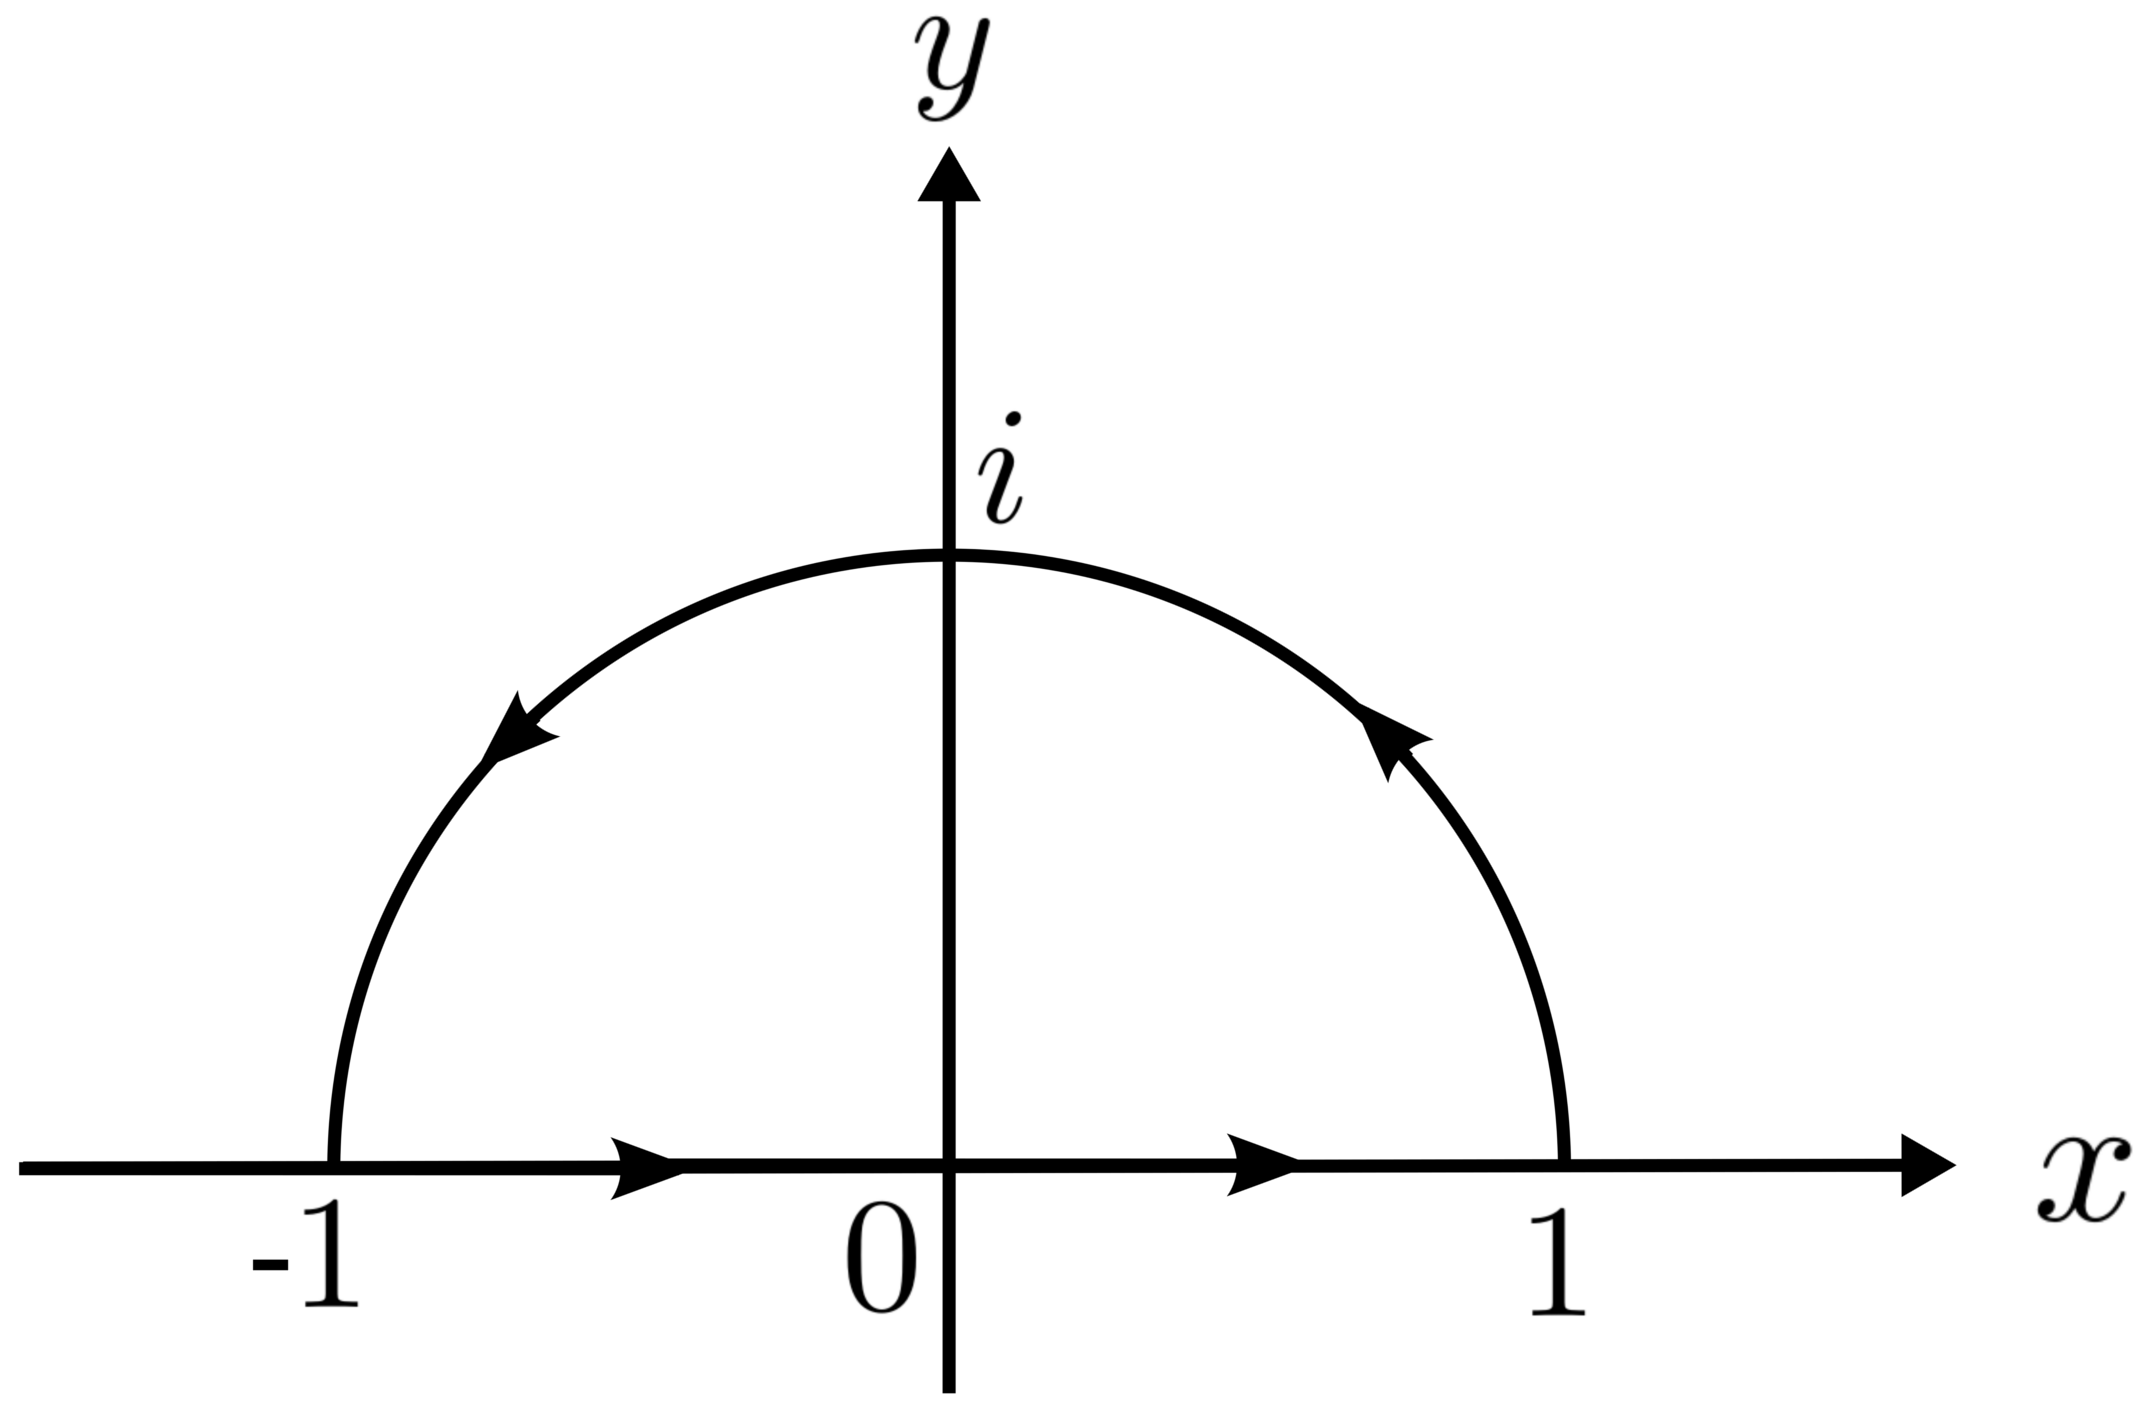
\includegraphics[width=0.35\textwidth]{6.png}
  \end{center}
\end{wrapfigure}



então $\gamma=\gamma_{0}\vee\gamma_{1}$ tem a seguinte

representação geométrica:\\

 \ \ \ \ \ \ \ \ \ \ \ \ \  \ \ \ \ \ \ \ \ \ \ \ \ \


Como $\gamma^{\prime}(  t)  =\left\{
\begin{array}
[c]{c}
ie^{it},\text{ \ se \ }0<t<\pi\\\\\genfrac{}{}{1pt}{0}{2}{\pi},\text{ \ se \ }\pi<t<2\pi
\end{array}
\right.$ ,\\


\bigskip


pela definição de $\underset{\gamma}{
{\displaystyle\int}
}\left\vert z\right\vert $
$\overline{z}dz$, \ temos:\\\\


$$\int_{\gamma} \left\vert z \right\vert \overline{z}dz \! = \!\int^{\pi}_0\!1\!\cdot\!e^{-it}\!\cdot\!i\cdot\!e^{it}dt  +  \underset{\pi}
{{\displaystyle\int}}^{2\pi}\left\vert \genfrac{}{}{1pt}{0}{2}{\pi} t-3\right\vert (\genfrac{}{}{1pt}{0}{2}{\pi} t-3) \genfrac{}{}{1pt}{0}{z}{\pi} dt$$

$=i\pi-\underset{\pi}{{\displaystyle\int}}^{3\pi/2}(\genfrac{}{}{1pt}{0}{2}{\pi}t-3)^{2}dt+\underset{3\pi/2}{{\displaystyle\int^{2\pi}}}(\genfrac{}
{}{1pt}{0}{2}{\pi}t-3) ^{2}dt = i\pi$

\bigskip
\bigskip
\bigskip

% IMAGEM 8
\begin{wrapfigure}{r}{0.17\textwidth}
  \begin{center}
    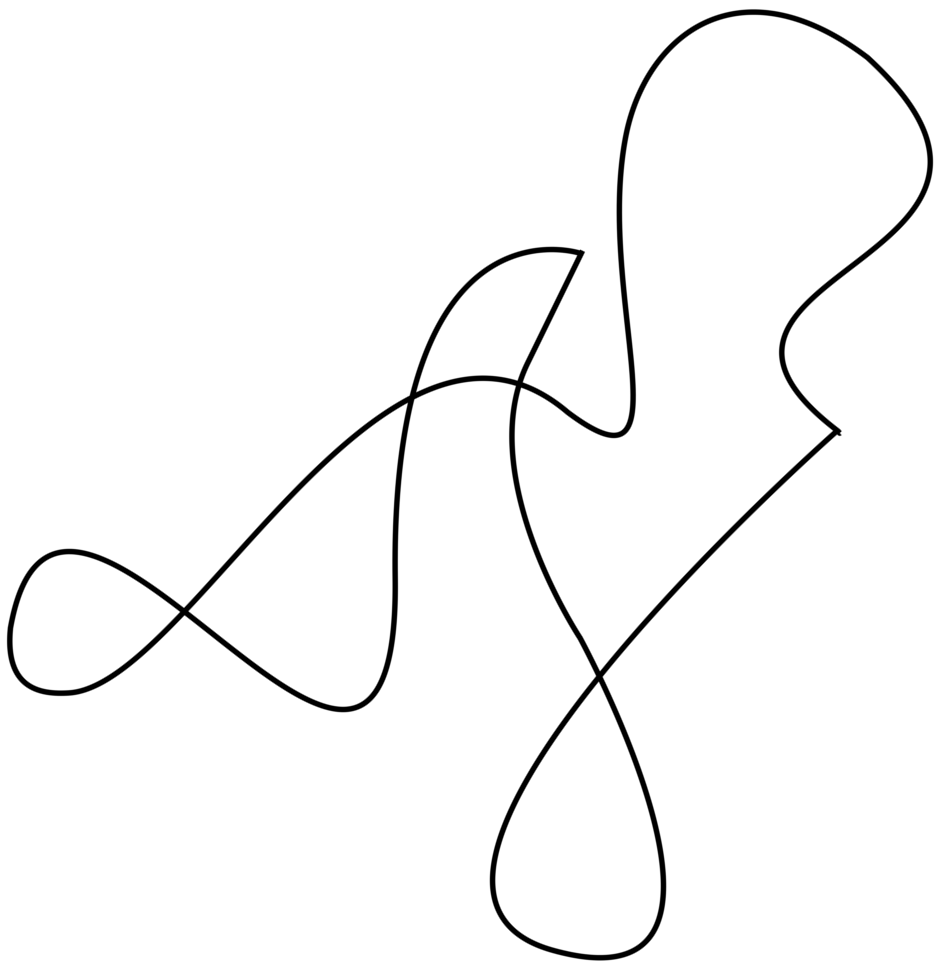
\includegraphics[width=0.17\textwidth]{8.png}
  \end{center}
\end{wrapfigure}


\textbf{Teorema 5.2 \ }\textit{Sejam }$\gamma:\left[  a,b\right]  \rightarrow\mathbb{C}$ \textit{uma CSDF em }$\mathbb{C}$,

$\Omega:$ $=\mathbb{C}\backslash\gamma^{\ast}$ \ \textit{e}\\\\


\ \ \ \ \ \ \ \ \ \ \ \ \ \ \ \ \ \ \ \ \ \textsc{I}nd$_{\gamma}:z\in\Omega\rightarrow\genfrac{}{}{1pt}{0}{1}{2\pi i}\underset{\gamma}{{\displaystyle\int}}\genfrac{}{}{1pt}{0}{d\zeta}{\zeta-z}\in\mathbb{C}$.

\bigskip\textit{Então, \textsc{I}}nd$_{\gamma}$\textit{\ é uma
função (definida em }$\Omega$) \textit{\ que toma}

\textit{valores inteiros, é constante em cada componente conexa}

\textit{de} $\Omega$ \textit{e que vale }$0$ \textit{sobre a componente conexa não limitada}

\textit{de} $\Omega$ (ver exercício (5.6)).

\bigskip

Para cada $z\in\Omega$ $\ $o número inteiro \textsc{I}nd$_{\gamma}$ é chamado \textit{índice de $z$ em relação}

\textit{a} $\gamma.$ Como $\gamma^{\ast}$ é compacto, é limitado e portanto existe um

disco fechado $D$ de raio finito tal que $\gamma^{\ast}\subset D.$ Em consequência, $W:=\mathbb{C}\backslash D$

é aberto, não vazio e obviamente $W$ é conexo e como $W\subset\Omega$ resulta (ver

Ex. (5.6) (f)) que W está contido numa componente conexa $\Omega_{0}$ de $\Omega$ que não

pode ser limitada pois $W$ não é limitado, o que prova a existência de uma

componente conexa não limitada de $\Omega_{0}$ de $\Omega.$Mostremos que $\Omega_{0}$ é a única

componente conexa não limitada de $\Omega$. De fato, $\Omega_{0}\supset W=\mathbb{C}\backslash D$, portanto

$\mathbb{C}\backslash\Omega_{0}\subset D$ e como as componentes conexas são duas a duas disjuntas, toda

outra componente conexa $\Omega_{1}$ de $\Omega$ está contida em $\mathbb{C}\backslash\Omega_{0}$ e portanto

em $D,$ donde $\Omega_{1}$ é limitada.

\bigskip

\textbf{Prova do Teorema 5.2\ }\ Fixemos $z\in\Omega$ arbitário e mostremos que

\textsc{I}nd$_{\gamma}(  z)$ $\in\mathbb{Z}$. Por definição temos:

\bigskip

$(  5.2.1)  $ \ \ \ \ \ \ \ \ \ \ \ \ \textsc{I}nd$_{\gamma}(
z)  =%
%TCIMACRO{\QDABOVE{1pt}{1}{2\pi i}}%
%BeginExpansion
\genfrac{}{}{1pt}{0}{1}{2\pi i}%
%EndExpansion
\underset{a}{%
%TCIMACRO{\dint }%
%BeginExpansion
{\displaystyle\int}
%EndExpansion
}^{b}%
%TCIMACRO{\QDABOVE{1pt}{\gamma^{\prime}(  s)  ds}{\gamma(
%s)  -z}}%
%BeginExpansion
\genfrac{}{}{1pt}{0}{\gamma^{\prime}(  s)  ds}{\gamma(
s)  -z}%
%EndExpansion
$

\bigskip

Pelo Teor. 3.14. (g) sabemos que para $w\in%
%TCIMACRO{\U{2102} }%
%BeginExpansion
\mathbb{C}
%EndExpansion
$ temos

\bigskip

\ \ \ \ \ \ \ \ \ \ \ \ \ \ \ \ \ \ \ \ \ \ \ \ \ \ \ \ $%
%TCIMACRO{\QDABOVE{1pt}{w}{2\pi i}}%
%BeginExpansion
\genfrac{}{}{1pt}{0}{w}{2\pi i}%
%EndExpansion
\in%
%TCIMACRO{\U{2124} }%
%BeginExpansion
\mathbb{Z}
%EndExpansion
\iff\exp(  w)  =1$

\bigskip

portanto de $(  5.2.1)  $ resulta que a relação
\textsc{I}nd$_{\gamma}(  z)  \in%
%TCIMACRO{\U{2124} }%
%BeginExpansion
\mathbb{Z}
%EndExpansion
$ \ é equivalente a

\bigskip

$(  5.2.2)  $ \ \ \ \ \ \ \ \ \ \ \ \ \ \ $\exp(  \underset
{a}{%
%TCIMACRO{\dint }%
%BeginExpansion
{\displaystyle\int}
%EndExpansion
}^{b}%
%TCIMACRO{\QDABOVE{1pt}{\gamma^{\prime}(  s)  ds}{\gamma(
%s)  -z}}%
%BeginExpansion
\genfrac{}{}{1pt}{0}{\gamma^{\prime}(  s)  ds}{\gamma(
s)  -z}%
%EndExpansion
)  =1$

\bigskip

Consideremos a função $\varphi$ definida por

\bigskip

$(  5.2.3)  $ \ \ \ \ \ \ \ \ \ \ \ \ \ \ \ \ $\varphi(
t)  =\exp(  \underset{a}{%
%TCIMACRO{\dint }%
%BeginExpansion
{\displaystyle\int}
%EndExpansion
}^{t}%
%TCIMACRO{\QDABOVE{1pt}{\gamma^{\prime}(  s)  ds}{\gamma(
%s)  -z}}%
%BeginExpansion
\genfrac{}{}{1pt}{0}{\gamma^{\prime}(  s)  ds}{\gamma(
s)  -z}%
%EndExpansion
)  ,$ \ \ \ \ \ \ \ $\forall$ \ $t\in\left[  a,b\right]  $

\bigskip

Derivando esta função obtemos

\bigskip

$(  5.2.4)  $ \ \ \ \ \ \ \ \ \ \ \ \ \ $\varphi^{\prime}(
t)  =%
%TCIMACRO{\QDABOVE{1pt}{\varphi(  t)  \cdot\varphi^{\prime}(
%t)  }{\gamma(  t)  -z}}%
%BeginExpansion
\genfrac{}{}{1pt}{0}{\varphi(  t)  \cdot\varphi^{\prime}(
t)  }{\gamma(  t)  -z}%
%EndExpansion
$

\bigskip

para cada $t\in\left[  a,b\right]  $ $\backslash S,$ onde $S$ é o conjunto
finito de pontos nos quais $\gamma$ não

é diferenciável. Calculando a derivada da função contínua:

\bigskip

\ \ \ \ \ \ \ \ \ \ \ \ \ \ \ \ \ \ \ \ \ $\psi:t\in\left[  a,b\right]
\longmapsto%
%TCIMACRO{\QDABOVE{1pt}{\varphi(  t)  }{\gamma(  t)
%-z}}%
%BeginExpansion
\genfrac{}{}{1pt}{0}{\varphi(  t)  }{\gamma(  t)  -z}%
%EndExpansion
\in%
%TCIMACRO{\U{2102} }%
%BeginExpansion
\mathbb{C}
%EndExpansion
$

\bigskip

obtemos $\ \ \psi^{\prime}(  t)  =%
%TCIMACRO{\QDABOVE{1pt}{\varphi^{\prime}(  t)  \left[  \gamma(
%t)  -z\right]  -\varphi(  t)  \gamma^{\prime}(
%t)  }{\left[  \gamma(  t)  -z\right]  ^{2}}}%
%BeginExpansion
\genfrac{}{}{1pt}{0}{\varphi^{\prime}(  t)  \left[  \gamma(
t)  -z\right]  -\varphi(  t)  \gamma^{\prime}(
t)  }{\left[  \gamma(  t)  -z\right]  ^{2}}%
%EndExpansion
$ \ , \ \ para cada \ \ \ $t\in\left[  a,b\right]  \backslash S,$ \ 

\bigskip

em consequência por $(  5.2.4)  $ resulta que

\bigskip\ \ \ \ \ \ \ \ \ \ \ \ \ \ \ \ \ \ \ \ \ \ \ \ \ \ $\psi^{\prime
}(  t)  =0$ \ \ \ \ para cada \ $t\in\left[  a,b\right]  \backslash
S $ \ ,

o que mostra que $\psi$ é uma função contínua em $\left[
a,b\right]  $ cuja derivada é nula em

$\left[  a,b\right]  \backslash S,$ logo, como $S$ é finito, resulta que
$\psi$ é constante em $\left[  a,b\right]  $ e como

por $(  5.2.3)  $ temos $\varphi(  a)  =1,$ resulta

\bigskip

\ \ \ \ \ \ \ \ \ \ \ \ \ \ \ \ \ \ \ \ \ \ \ \ \ \ \ \ \ \ \ \ \ \ \ \ \ $\psi
(  a)  =%
%TCIMACRO{\QDABOVE{1pt}{1}{\gamma(  a)  -z}}%
%BeginExpansion
\genfrac{}{}{1pt}{0}{1}{\gamma(  a)  -z}%
%EndExpansion
.$

\bigskip

De $\psi(  t)  =\psi(  a)  $ \ $\forall$ \ $t\in\left[
a,b\right]  $ resulta então por definição de $\psi:$

\bigskip

$(  5.2.5)  $ \ \ \ \ \ \ \ \ \ \ \ \ $\varphi(  t)  =%
%TCIMACRO{\QDABOVE{1pt}{\gamma(  t)  -z}{\gamma(  a)
%-z}}%
%BeginExpansion
\genfrac{}{}{1pt}{0}{\gamma(  t)  -z}{\gamma(  a)  -z}%
%EndExpansion
$ \ \ $\forall$ \ $t\in\left[  a,b\right]  $

\bigskip

e como $\gamma$ é fechada, isto é, $\gamma(  a)
=\gamma(  b)  ,$ de $(  5.2.5)  $ resulta $\varphi
(  b)  =1,$ ou seja

$(  5.2.2)  ,$ o que prova que \textsc{I}nd$_{\gamma}(
z)  \in%
%TCIMACRO{\U{2124} }%
%BeginExpansion
\mathbb{Z}
%EndExpansion
.$

Como $(  5.2.1)  $ vale para cada $z\in\Omega,$ o Teor. 4.3 implica

\ \ \ \ \ \ \ \ \ \ \ \ \ \ \ \ \ \ \ \ \ \ \ \ \ \ \ \ \ \ \ \ \ \ 

\ \ \ \ \ \ \ \ \ \ \ \ \ \ \ \ \ \ \ \ \ \ \ \ \ \ \ \ \ \ \ \ \ \ \textsc{I}%
nd$_{\gamma}\in\mathcal{A}(  \Omega)  $

donde \textsc{I}nd$_{\gamma}\in\mathcal{C}(  \Omega)  .$ Como a
imagem de um conexo por uma função contínua

é um conjunto conexo, resulta que se $V$ é uma componente conexa de
$\Omega,$

então \ \textsc{I}nd$_{\gamma}(  V)  $ \ é um subconjunto
conexo de $%
%TCIMACRO{\U{2102} }%
%BeginExpansion
\mathbb{C}
%EndExpansion
.$ Ora, \ já \ vimos \ que

\textsc{I}nd$_{\gamma}(  z)  \in%
%TCIMACRO{\U{2124} }%
%BeginExpansion
\mathbb{Z}
%EndExpansion
$ \ para cada $z\in\Omega,$ portanto

\bigskip

\ \ \ \ \ \ \ \ \ \ \ \ \ $\varnothing\neq$ \textsc{I}nd$_{\gamma}(
V)  \subset%
%TCIMACRO{\U{2124} }%
%BeginExpansion
\mathbb{Z}
%EndExpansion
$ \ \ \ \ \ \ \ e \ \ \ \ \ \ \ \ \textsc{I}nd$_{\gamma}(  V)  $
\ \ é conexo,

e como os únicos subconjuntos não vazios de $%
%TCIMACRO{\U{2124} }%
%BeginExpansion
\mathbb{Z}
%EndExpansion
$ que são conexos (no espaço

topológico $%
%TCIMACRO{\U{2102} }%
%BeginExpansion
\mathbb{C}
%EndExpansion
$) são aqueles que têm apenas um elemento, existe $k\in%
%TCIMACRO{\U{2124} }%
%BeginExpansion
\mathbb{Z}
%EndExpansion
$ \ tal

que \textsc{I}nd$_{\gamma}(  V)  =\left\{  k\right\}  ,$ o que
prova que

\ \ \ \ \ \ \ \ \ \ \ \ \ \ \ \ \ \ \ \ 

\ \ \ \ \ \ \ \ \ \ \ \ \ \ \ \ \ \ \ \ \ \ \ \ \ \ \ \ \ \ \ \textsc{I}%
nd$_{\gamma}(  z)  =k$ \ \ para cada \ $z\in V,$

isto é, \textsc{I}nd$_{\gamma}$ é constante sobre cada componente
conexa de $\Omega.$ Mostremos

finalmente \ que \textsc{I}nd$_{\gamma}$ se anula sobre a componente conexa
não limitada $\Omega_{0}$ \ 

de $\Omega.$ Se $\rho>0$ é o raio de um disco de centro $0$ contendo
$\gamma^{\ast},$ \ então

\bigskip

\ \ \ \ \ \ \ \ \ \ \ \ \ \ \ $\left\vert
%TCIMACRO{\QDABOVE{1pt}{\gamma(  s)  }{z}}%
%BeginExpansion
\genfrac{}{}{1pt}{0}{\gamma(  s)  }{z}%
%EndExpansion
\right\vert <%
%TCIMACRO{\QDABOVE{1pt}{1}{2}}%
%BeginExpansion
\genfrac{}{}{1pt}{0}{1}{2}%
%EndExpansion
,$ \ \ $\forall$ \ $s\in\left[  a,b\right]  $ \ \ e \ \ $\forall$
\ $x\in\Omega,$ \ $\left\vert z\right\vert >2\rho$

donde

\ \ \ \ \ \ \ \ \ \ \ \ \ \ $\left\vert \left\vert
%TCIMACRO{\QDABOVE{1pt}{\gamma(  s)  }{z}}%
%BeginExpansion
\genfrac{}{}{1pt}{0}{\gamma(  s)  }{z}%
%EndExpansion
\right\vert -1\right\vert =1-\left\vert
%TCIMACRO{\QDABOVE{1pt}{\gamma(  s)  }{z}}%
%BeginExpansion
\genfrac{}{}{1pt}{0}{\gamma(  s)  }{z}%
%EndExpansion
\right\vert >%
%TCIMACRO{\QDABOVE{1pt}{1}{2}}%
%BeginExpansion
\genfrac{}{}{1pt}{0}{1}{2}%
%EndExpansion
,$ \ \ $\forall$ \ $s\in\left[  a,b\right]  $ \ \ \ e \ \ \ $\forall$
\ $\left\vert z\right\vert >2\rho$

o que implica

\ \ \ \ \ \ \ \ \ \ \ \ \ \ $\left\vert \text{\textsc{I}nd}_{\gamma}(
z)  \right\vert \leq%
%TCIMACRO{\QDABOVE{1pt}{1}{2\pi\left\vert z\right\vert }}%
%BeginExpansion
\genfrac{}{}{1pt}{0}{1}{2\pi\left\vert z\right\vert }%
%EndExpansion
\underset{a}{%
%TCIMACRO{\dint }%
%BeginExpansion
{\displaystyle\int}
%EndExpansion
}^{b}%
%TCIMACRO{\QDABOVE{1pt}{\left\vert \gamma^{\prime}(  s)  \right\vert
%ds}{\left\vert \left\vert \QDABOVE{1pt}{\gamma(  s)  }%
%{z}\right\vert -1\right\vert }}%
%BeginExpansion
\genfrac{}{}{1pt}{0}{\left\vert \gamma^{\prime}(  s)  \right\vert
ds}{\left\vert \left\vert \genfrac{}{}{1pt}{0}{\gamma(  s)
}{z}\right\vert -1\right\vert }%
%EndExpansion
\leq%
%TCIMACRO{\QDABOVE{1pt}{1}{\pi\left\vert z\right\vert }}%
%BeginExpansion
\genfrac{}{}{1pt}{0}{1}{\pi\left\vert z\right\vert }%
%EndExpansion
\left\vert \gamma\right\vert ,$ \ \ se \ \ \ $\left\vert z\right\vert >2\rho.$

\bigskip

Como $\Omega_{0}$ não é limitada existe $z\in\Omega_{0}$ tal que

\ \ \ \ \ \ \ \ \ \ \ \ \ \ \ \ \ \ \ \ \ \ 

\ \ \ \ \ \ \ \ \ \ \ \ \ \ \ \ \ \ \ \ \ \ \ \ \ \ $\left\vert z\right\vert
>\max(  2\rho,%
%TCIMACRO{\QDABOVE{1pt}{\left\vert \gamma\right\vert }{\pi}}%
%BeginExpansion
\genfrac{}{}{1pt}{0}{\left\vert \gamma\right\vert }{\pi}%
%EndExpansion
)  $

e então \ $\left\vert \text{\textsc{I}nd}_{\gamma}(  z)
\right\vert <1,$ \ logo \textsc{I}nd$_{\gamma}(  z)  =0.$ Como
\textsc{I}nd$_{\gamma}$ é constante em $\Omega_{0},$

resulta \textsc{I}nd$_{\gamma}(  w)  =0$ \ para cada $w\in
\Omega_{0}.$ \ $\square$

\bigskip

Na oBservação abaixo usaremos o argumento de um número complexo na sua forma intuitiva (ver Def. 6.9).

\textbf{Observação \ }Seja $\gamma:\left[  a,b\right]  \rightarrow%
%TCIMACRO{\U{2102} }%
%BeginExpansion
\mathbb{C}
%EndExpansion
$ uma CSDF. Se interpretamos fisicamente

$\gamma(  t)  $ como a posição de uma partícula
móvel no instante $t,$ o Teor. 5.2 tem

uma interpretação física correspondente como o número de
vezes que a

partícula gira em volta do ponto $z\notin\gamma^{\ast}$ dado. De fato,
com as notações do

Teor. 5.2 \ fixemos $z\in\Omega$ arbitrário, então

\bigskip

\ \ \ \ \ \ \ \ \ \ \ \ \ \textsc{I}nd$_{\gamma}(  z)  =%
%TCIMACRO{\QDABOVE{1pt}{1}{2\pi i}}%
%BeginExpansion
\genfrac{}{}{1pt}{0}{1}{2\pi i}%
%EndExpansion
\underset{a}{%
%TCIMACRO{\dint }%
%BeginExpansion
{\displaystyle\int}
%EndExpansion
}^{b}%
%TCIMACRO{\QDABOVE{1pt}{\gamma^{\prime}(  s)  ds}{\gamma(
%s)  -z}}%
%BeginExpansion
\genfrac{}{}{1pt}{0}{\gamma^{\prime}(  s)  ds}{\gamma(
s)  -z}%
%EndExpansion
=k\in%
%TCIMACRO{\U{2124} }%
%BeginExpansion
\mathbb{Z}
%EndExpansion
,$

portanto, se

\ \ \ \ \ \ \ \ \ \ \ \ \ \ \ \ \ \ \ \ \ \ \ \ \ \ \ \ \ \ \ \ \ $\lambda
(  t)  :=\underset{a}{%
%TCIMACRO{\dint }%
%BeginExpansion
{\displaystyle\int}
%EndExpansion
}^{t}%
%TCIMACRO{\QDABOVE{1pt}{\gamma^{\prime}(  s)  ds}{\gamma(
%s)  -z}}%
%BeginExpansion
\genfrac{}{}{1pt}{0}{\gamma^{\prime}(  s)  ds}{\gamma(
s)  -z}%
%EndExpansion
$ \ \ \ \ $\forall$ \ \ $t\in\left[  a,b\right]  $

podemos escrever

\ \ \ \ \ \ \ \ \ \ \ \ \ \ \ \ \ \ \ \ \ \ \ \ \ \ \ \ \ \ \ \ \ \ $2\pi$
\textsc{I}nd$_{\gamma}(  z)  =%
%TCIMACRO{\QDABOVE{1pt}{1}{i}}%
%BeginExpansion
\genfrac{}{}{1pt}{0}{1}{i}%
%EndExpansion
\lambda(  b)  =2k\pi$

Sejam $\lambda_{1}:=\operatorname{Re}(  \lambda)  $ \ e
$\lambda_{2}:=\operatorname{Im}(  \lambda)  $ \ isto é
$\ \lambda(  b)  =\lambda_{1}(  b)  +i\lambda_{2}(
b)  $ \ logo de

$%
%TCIMACRO{\QDABOVE{1pt}{1}{i}}%
%BeginExpansion
\genfrac{}{}{1pt}{0}{1}{i}%
%EndExpansion
\lambda(  b)  =2k\pi$ \ resulta que $\lambda(  b)  $
é imaginário puro, ou seja $\lambda(  b)  =i\lambda
_{2}(  b)  $

(isto é, $\lambda_{1}(  b)  =0$), donde

\ \ \ \ \ \ \ \ \ \ \ \ \ \ \ \ \ \ \ \ \ \ \ \ \ \ \ \ \ $2\pi$%
\textsc{I}nd$_{\gamma}(  z)  =-i\lambda(  b)
=2k\pi=\lambda_{2}(  b)  $

o que implica \ \ \ (observe que $\lambda_{2}(  b)  =\lambda
_{2}(  b)  -\lambda_{2}(  a)  $ \ pois $\lambda(
a)  =0\implies$

$\lambda_{2}(  a)  =0)$

\bigskip

$\left[  1\right]  $ \ \ \ \ \ \ \ \ $\left\Vert
\begin{array}
[c]{c}%
\lambda_{2}(  b)  =2\pi\text{\textsc{I}nd}_{\gamma}(
z)  =\text{aumento total da parte}\\
\text{imaginária }\lambda_{2}\text{ de }\lambda\text{ quando }t\text{
varia de }a\text{ até }b
\end{array}
\right.  $

\bigskip

Por outro lado, de $(  5.2.5)  $ $\ \ \ (  \varphi(
t)  =%
%TCIMACRO{\QDABOVE{1pt}{\gamma(  t)  -z}{\gamma(  a)
%-z}}%
%BeginExpansion
\genfrac{}{}{1pt}{0}{\gamma(  t)  -z}{\gamma(  a)  -z}%
%EndExpansion
)  $ \ \ segue

\bigskip

$\left[  2\right]  $ \ \ \ \ \ \ \ \ $\left\Vert \text{ }\arg\left[
\varphi(  t)  \right]  \right.  =\arg\left[  \gamma(
t)  -z\right]  -\arg\left[  \gamma(  a)  -z\right]  $

\bigskip

e como $\varphi(  t)  =\exp\left[  \lambda(  t)
\right]  $ \ \ $\forall$ \ $t\in\left[  a,b\right]  ,$ \ resulta
\ \ $\varphi(  b)  =\exp\left[  \lambda(  b)  \right]
=$

$\exp\left[  i\lambda_{2}(  b)  \right]  ,$ \ o que implica
(lembrar que $\arg(  e^{ix})  =x$ \ \ $\forall$ \ $x\in%
%TCIMACRO{\U{211d} }%
%BeginExpansion
\mathbb{R}
%EndExpansion
$)

\bigskip

$\left[  3\right]  $ \ \ \ \ \ \ \ \ $\left\Vert \text{ }\arg\left[
\varphi(  b)  \right]  \right.  =\arg\left[  \exp(
i\lambda_{2}(  b)  )  \right]  =\lambda_{2}(  b)
$

\bigskip

Igualando os últimos termos de $\left[  2\right]  $ \ $(  t=b)
$ \ e \ $\left[  3\right]  :$

\bigskip

$\left[  4\right]  $ \ \ \ \ \ \ \ \ $\left\Vert
\begin{array}
[c]{c}%
\lambda_{2}(  b)  =\arg\left[  \gamma(  b)  -z\right]
-\arg\left[  \gamma(  a)  -z\right]  =\text{aumento total}\\
\text{do argumento de }\gamma(  t)  -z\text{ quando }t\text{ varia
de }a\text{ até }b\text{ }%
\end{array}
\right.  $

\bigskip

De $\left[  1\right]  $ e $\left[  4\right]  $ segue então\ \ \ \ \ \ \ \ \ \ \ \ \ \ \ \ \ \ \ \ \ \ \ \ \ \ \ \ \ \ \ \ \ \ \ 

\bigskip

\ \ \ \ \ \ \ \ \ \ \ \ \ $\left\Vert
\begin{array}
[c]{c}%
2\pi\text{ \textsc{I}}nd_{\gamma}(  z)  =\text{aumento total do
argumento de }\gamma(  t)  -z\\
\text{quando }t\text{ varia de }a\text{ até }b=2k\pi\text{
\ \ \ \ \ \ \ \ \ \ \ \ \ \ \ \ \ \ \ \ \ \ \ \ \ \ \ \ \ \ \ \ \ }%
\end{array}
\right.  $\ \ \ 

\ \ \ \ \ \ \ \ \ \ \ \ \ \ \ \ \ \ 

e então, dividindo ambos membros da igualdade anterior por $2\pi,$ obtemos

o número inteiro

\ \ \ \ \ \ \ \ \ \ \ \ \ \ \ \ \ \ \ \ \ \ \ \ \ \ \ \ \ \ \ \ \ \ \ \ \textsc{I}%
nd$_{\gamma}(  z) =k$\\

que pode ser interpretado como \textit{o número de vezes que a partícula móvel}

$\gamma(t)$ \textit{gira em volta de $z$ quando $t$ varia de $a$ até} $b$, ou como se diz mais

frequentemente, \textit{o número de vezes que $\gamma$ gira em volta de $z$ quando $t$}

\textit{varia de $a$ até} $b$.

% IMAGEM 9

\begin{center}
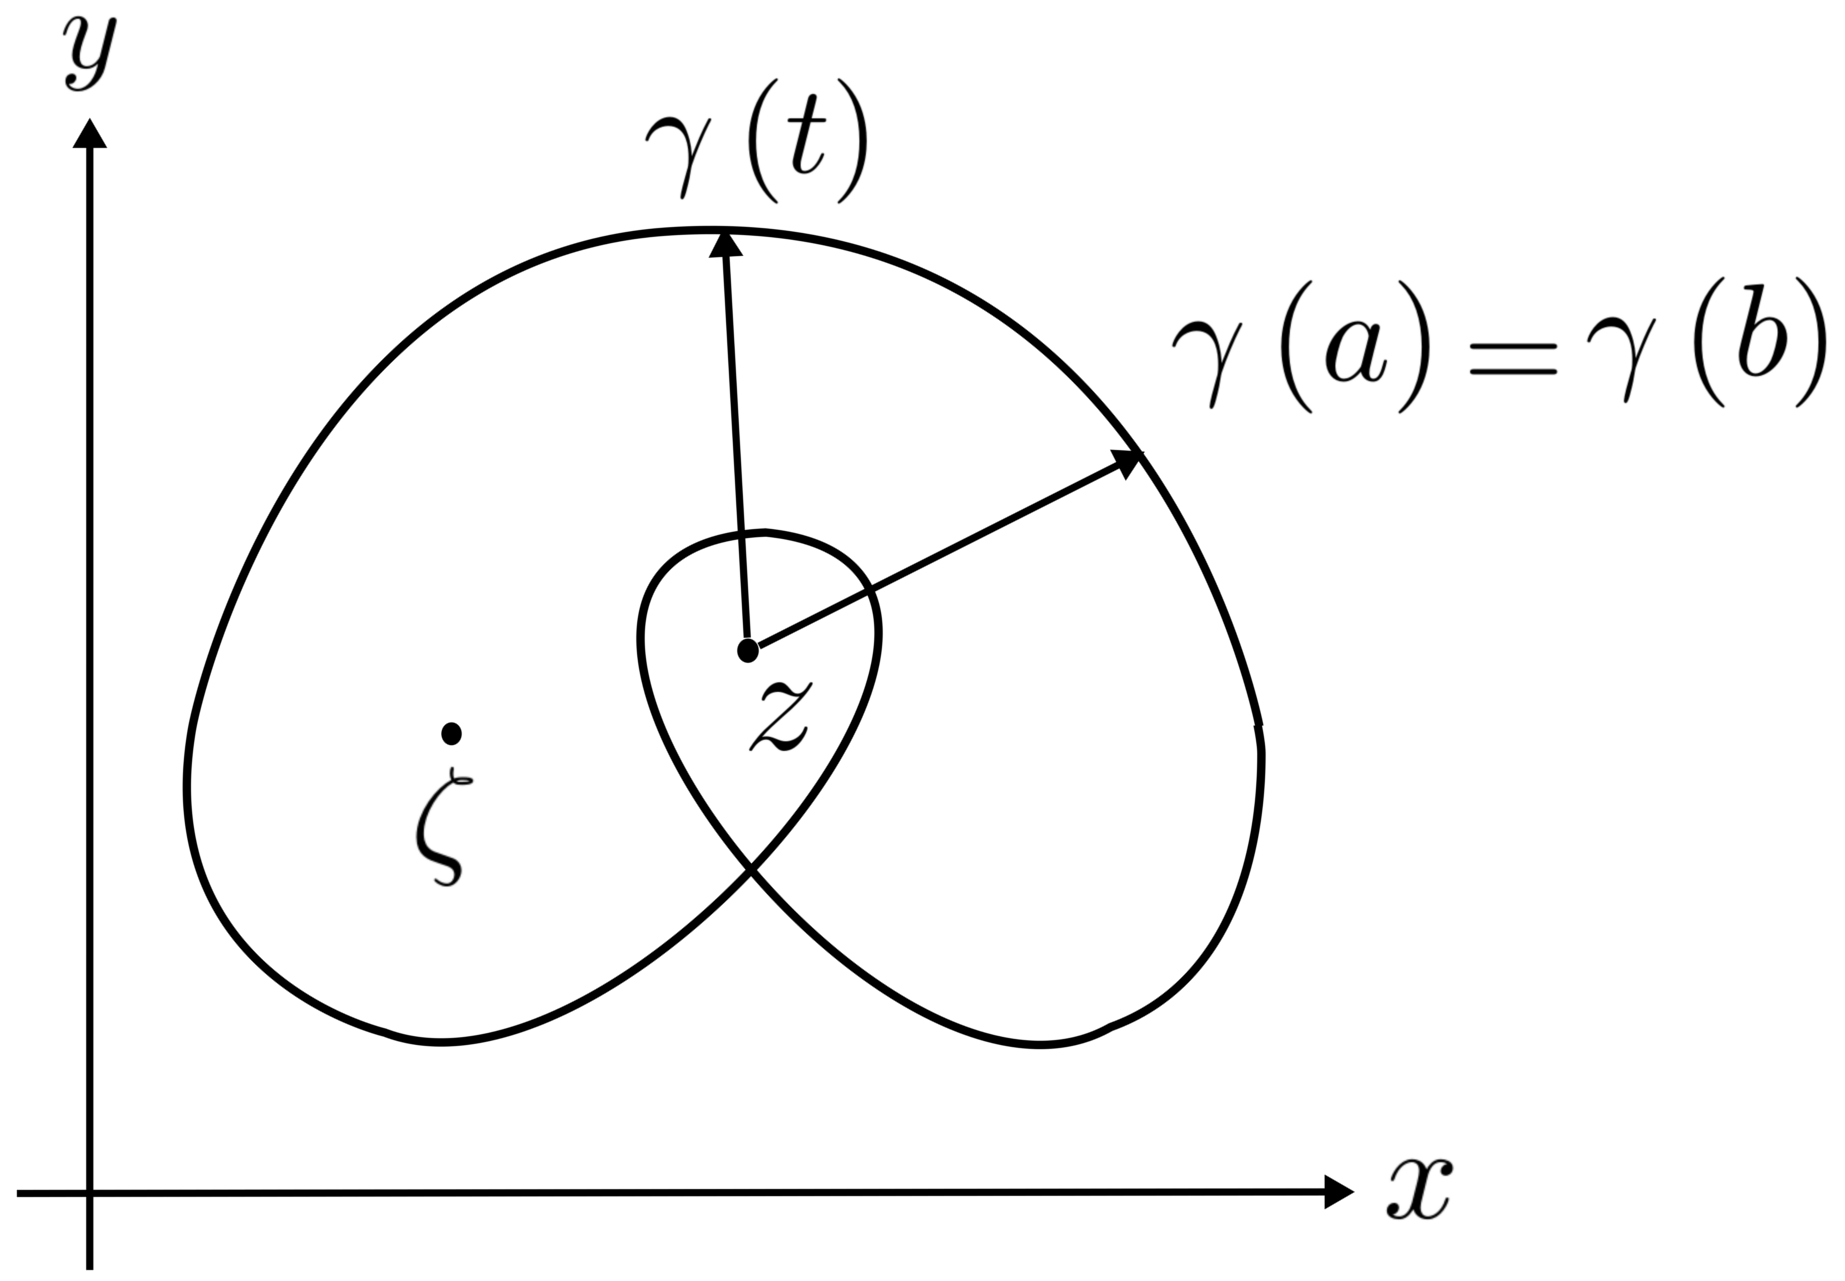
\includegraphics{9.png}
\end{center}


O caso particular seguinte é importante para o que segue:

\bigskip

\textbf{Proposição 5.3} \ \textit{Se }$\gamma$ \textit{é o
círculo orientado positivamente de centro }$\zeta$ \textit{e}

\textit{raio }$r>0$ (ver Casos Especiais, (a)), \textit{então:}

\bigskip\ \ \ \ \ \ \ \ \ \ \ \ \ \ \ \ \ \ \ \ \ \ \ \ \ \ \textsc{I}%
nd$_{\gamma}(  z)  =\left\{
\begin{array}
[c]{c}%
1,\text{\ se }\left\vert z-\zeta\right\vert <r\\
\\
0,\text{ se }\left\vert z-\zeta\right\vert >r
\end{array}
\right.  $

\bigskip\textbf{Prova \ }O aberto $\Omega=%
%TCIMACRO{\U{2102} }%
%BeginExpansion
\mathbb{C}
%EndExpansion
\backslash$ $\gamma^{\ast}$ tem duas componentes conexas que são

\ \ \ \ \ \ \ \ \ \ \ \ \ \ $\Omega_{1}=D_{r}(  \zeta)  $ \ \ e
\ \ \ $\Omega_{2}=\left\{  z\in%
%TCIMACRO{\U{2102} }%
%BeginExpansion
\mathbb{C}
%EndExpansion
\text{ }|\text{ }\left\vert z-\zeta\right\vert >r\right\}  $

\ e como \textsc{I}nd$_{\gamma}$ se anula sobre $\Omega_{2}$ (pelo Teor. 5.2
pois $\Omega_{2}$ é a componente

conexa não limitada de $\Omega$), basta ver que \textsc{I}nd$_{\gamma
}(  \zeta)  =1$ (pois \textsc{I}nd$_{\gamma}$ é cons-

tante sobre $\Omega_{1}$ pelo Teor. 5.2). De fato,

\bigskip

\ \ \ \ \ \ \ \ \ \ \ \ \ \textsc{I}nd$_{\gamma}(  \zeta)  =%
%TCIMACRO{\QDABOVE{1pt}{1}{2\pi i}}%
%BeginExpansion
\genfrac{}{}{1pt}{0}{1}{2\pi i}%
%EndExpansion
\underset{\gamma}{%
%TCIMACRO{\dint }%
%BeginExpansion
{\displaystyle\int}
%EndExpansion
}%
%TCIMACRO{\QDABOVE{1pt}{dz}{z-\zeta}}%
%BeginExpansion
\genfrac{}{}{1pt}{0}{dz}{z-\zeta}%
%EndExpansion
=%
%TCIMACRO{\QDABOVE{1pt}{ri}{2\pi i}}%
%BeginExpansion
\genfrac{}{}{1pt}{0}{ri}{2\pi i}%
%EndExpansion
\underset{0}{%
%TCIMACRO{\dint }%
%BeginExpansion
{\displaystyle\int}
%EndExpansion
}^{2\pi}%
%TCIMACRO{\QDABOVE{1pt}{e^{it}dt}{re^{it}}}%
%BeginExpansion
\genfrac{}{}{1pt}{0}{e^{it}dt}{re^{it}}%
%EndExpansion
=1.$ \ $\square$

\bigskip


\textbf{Exemplo 1} \ Se considera a CSDF \ $\Gamma:\left[  0,4\pi\right]
\rightarrow%
%TCIMACRO{\U{2102} }%
%BeginExpansion
\mathbb{C}
%EndExpansion
$ \ definida por
\bigskip\ \ \ \ \ \ \ \ \ \ \ \ \ \ \ \ \ \ \
\ \ \ \ \ \ \ \ \ \ \

% IMAGEM 10
\begin{wrapfigure}[1]{r}{0.2\textwidth}
  \begin{center}
    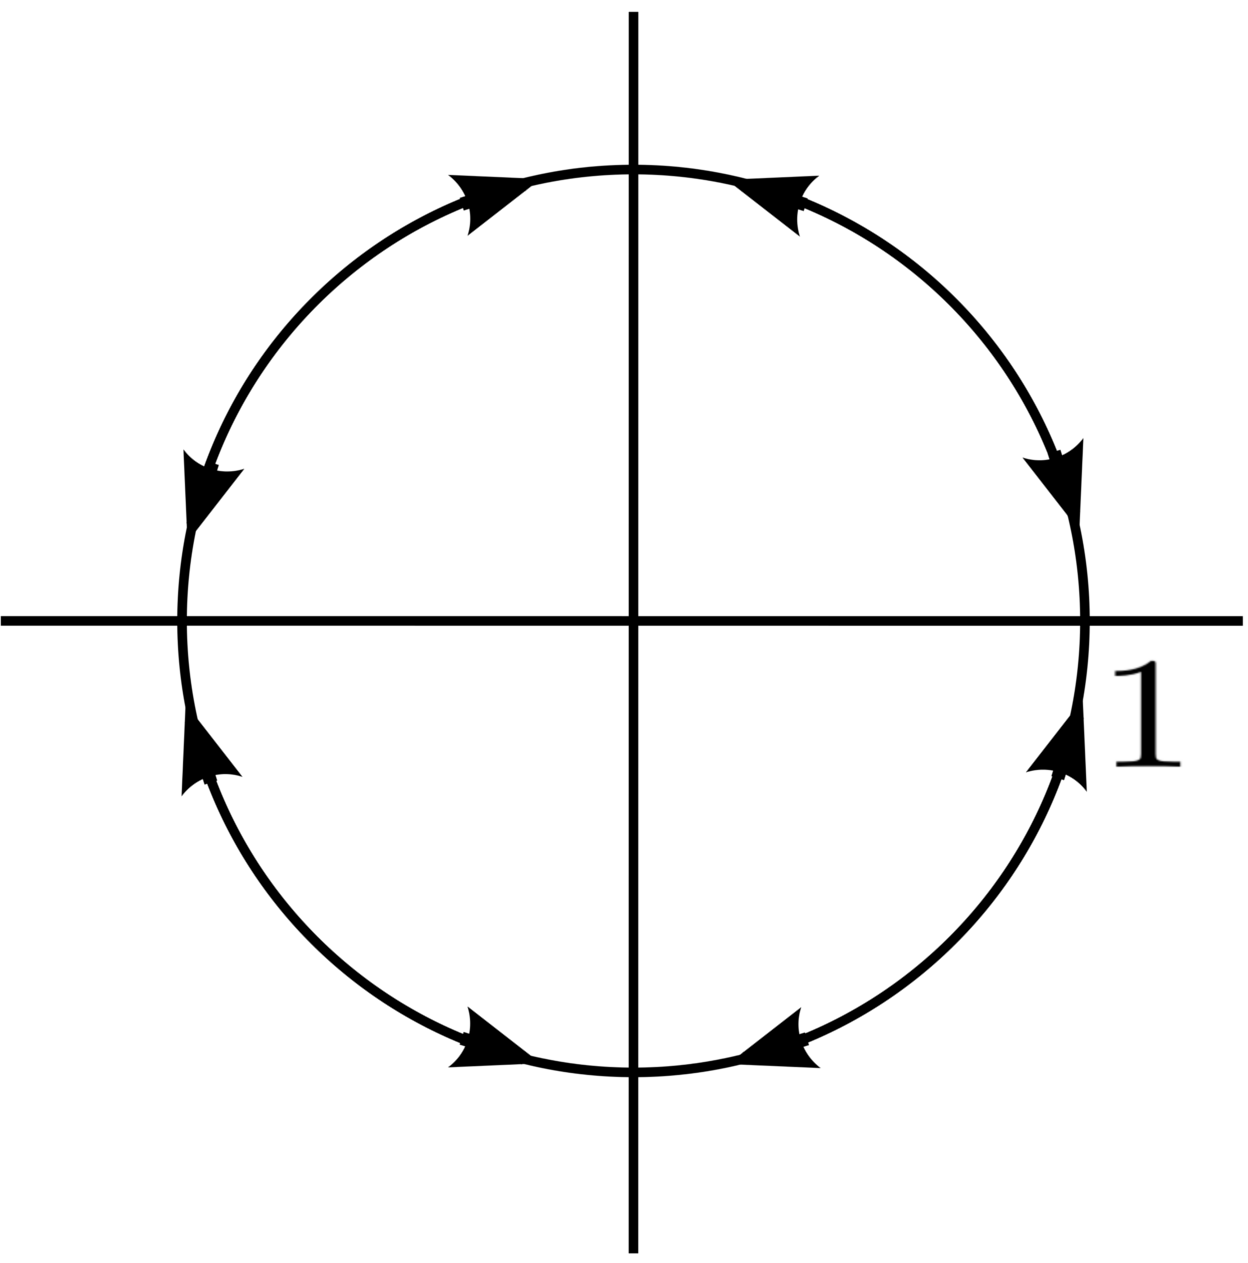
\includegraphics[width=0.2\textwidth]{10.png}
  \end{center}
\end{wrapfigure}

 $\Gamma(  t)
=\left\{
\begin{array}
[c]{c}%
e^{it},\text{ \ se \ }t\in\left[  0,2\pi\right]  \text{ \ \ }\\
\\
e^{-it},\text{ \ se \ }t\in\left[  2\pi,4\pi\right]
\end{array}
\right\}  $

\bigskip


Vamos mostrar que \textsc{I}nd$_{\Gamma}\equiv0.$ De fato, é claro que

\textsc{I}nd$_{\Gamma}(  z)  =0$ se $\left\vert
z\right\vert >1$ pela última asseção

do Teor. 5.2. Para provar que \textsc{I}nd$_{\Gamma}(  z)  =0$

sempre que $\left\vert z\right\vert <1,$ basta ver que \textsc{I}nd$_{\Gamma}(  0)  =0$,

o que é imediato.\\


\textsc{I}nd$_{\Gamma}(  0)  =%
%TCIMACRO{\QDABOVE{1pt}{1}{2\pi i}}%
%BeginExpansion
\genfrac{}{}{1pt}{0}{1}{2\pi i}%
%EndExpansion
\underset{\Gamma}{%
%TCIMACRO{\dint }%
%BeginExpansion
{\displaystyle\int}
%EndExpansion
}%
%TCIMACRO{\QDABOVED{.}{.}{1pt}{d\zeta}{\zeta}}%
%BeginExpansion
\genfrac{.}{.}{1pt}{0}{d\zeta}{\zeta}%
%EndExpansion
=%
%TCIMACRO{\QDABOVE{1pt}{1}{2\pi i}}%
%BeginExpansion
\genfrac{}{}{1pt}{0}{1}{2\pi i}%
%EndExpansion
\left[  \underset{0}{%
%TCIMACRO{\dint }%
%BeginExpansion
{\displaystyle\int}
%EndExpansion
}^{2\pi}%
%TCIMACRO{\QDABOVE{1pt}{ie^{it}dt}{e^{it}}}%
%BeginExpansion
\genfrac{}{}{1pt}{0}{ie^{it}dt}{e^{it}}%
%EndExpansion
+\underset{2\pi}{%
%TCIMACRO{\dint }%
%BeginExpansion
{\displaystyle\int}
%EndExpansion
}^{4\pi}%
%TCIMACRO{\QDABOVE{1pt}{-ie^{it}}{e^{-it}}}%
%BeginExpansion
\genfrac{}{}{1pt}{0}{-ie^{it}}{e^{-it}}%
%EndExpansion
dt\right]=0$

\bigskip

\textbf{Exemplo 2} \ Estudar a função \textsc{I}nd$_{\Gamma}$ sendo
$\Gamma:\left[  0,12\pi\right]  \rightarrow%
%TCIMACRO{\U{2102} }%
%BeginExpansion
\mathbb{C}
%EndExpansion
$

 a CSDF definida por


% IMAGEM 11
\begin{wrapfigure}{r}{0.4\textwidth}
  \begin{center}
    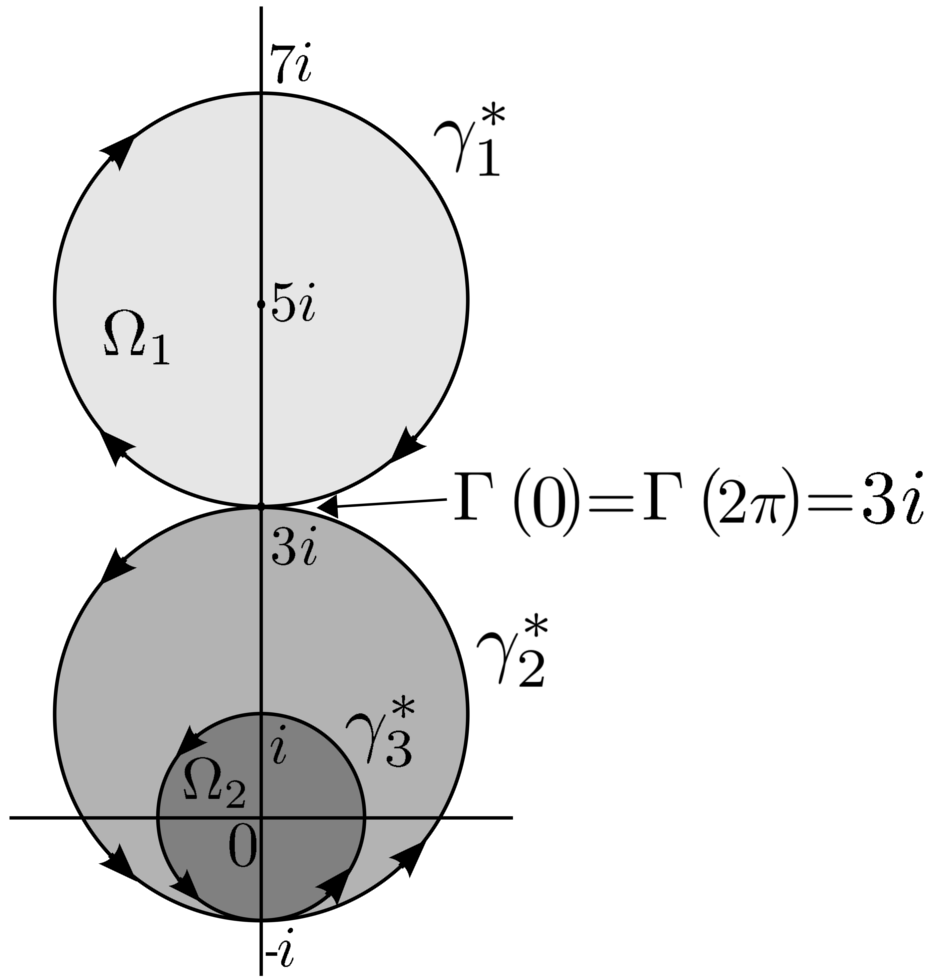
\includegraphics[width=0.4\textwidth]{11.png}
  \end{center}
\end{wrapfigure}

\ \ \ $\Gamma(  t)  :=\left\{
\begin{array}
[c]{c}%
\gamma_{1}(  t)  =5i-2ie^{-it}\text{ , \ \ \ se \ \ }t\in\left[
0,2\pi\right]  \text{ }\\
\gamma_{2}(  t)  =i+2ie^{it}\text{ , \ \ \ se \ \ \ }t\in\left[
2\pi,3\pi\right]  \text{ }\\
\gamma_{3}(  t)  =ie^{it}\text{ \ \ \ , \ \ \ se \ \ \ \ }%
t\in\left[  3\pi,9\pi\right]  \text{ \ \ \ }\\
\gamma_{2}(  t)  \text{ \ \ \ \ , \ \ \ \ \ se\ \ \ \ \ }%
t\in\left[  9\pi,10\pi\right]  \text{ \ \ \ \ \ \ \ \ }\\
\gamma_{1}(  t)  \text{ \ \ \ \ ,\ \ \ \ \ \ se \ \ \ }t\in\left[
10\pi,12\pi\right]  \text{ \ \ \ \ \ \ \ }%
\end{array}
\right.  $

\bigskip

\bigskip

As componentes conexas de $\Omega=%
%TCIMACRO{\U{2102} }%
%BeginExpansion
\mathbb{C}
%EndExpansion
\backslash$ $\Gamma^{\ast}$ \ 

são

$\Omega_{1}=$ disco aberto de fronteira $\gamma_{1}^{\ast}$

$\Omega_{2}=$ disco aberto de fronteira $\gamma_{3}^{\ast}$

$\Omega_{3}=$ disco aberto de fronteira $\gamma_{2}^{\ast}$

\ \ \ \ \ \ \ \ \ menos $\Omega_{2}\cup\gamma_{3}^{\ast}$

$\Omega_{4}=$ componente ilimitada de $\Omega$

\bigskip

\bigskip

\underline{\textsc{I}nd$_{\Gamma}$ em $\Omega_{1}$}:

\ \ \ \ \ \ \ \ \ \ \ \ \ \ \ \ \ \ \ \ \ \ Basta calcular \textsc{I}%
nd$_{\Gamma}(  5i)  .$

\bigskip

\textsc{I}nd$_{\Gamma}(  5i)  =%
%TCIMACRO{\QDABOVE{1pt}{1}{2\pi i}}%
%BeginExpansion
\genfrac{}{}{1pt}{0}{1}{2\pi i}%
%EndExpansion
\underset{0}{%
%TCIMACRO{\dint }%
%BeginExpansion
{\displaystyle\int}
%EndExpansion
}^{12\pi}%
%TCIMACRO{\QDABOVE{1pt}{\Gamma^{\prime}(  t)  dt}{\Gamma(
%t)  -5i}}%
%BeginExpansion
\genfrac{}{}{1pt}{0}{\Gamma^{\prime}(  t)  dt}{\Gamma(
t)  -5i}%
%EndExpansion
=%
%TCIMACRO{\QDABOVE{1pt}{1}{2\pi i}}%
%BeginExpansion
\genfrac{}{}{1pt}{0}{1}{2\pi i}%
%EndExpansion
\left\{  \underset{0}{%
%TCIMACRO{\dint }%
%BeginExpansion
{\displaystyle\int}
%EndExpansion
}^{2\pi}+\underset{2\pi}{%
%TCIMACRO{\dint }%
%BeginExpansion
{\displaystyle\int}
%EndExpansion
}^{10\pi}+\underset{10\pi}{%
%TCIMACRO{\dint ^{12\pi}}%
%BeginExpansion
{\displaystyle\int^{12\pi}}
%EndExpansion
}\right\}  $

\bigskip

$%
%TCIMACRO{\QDABOVE{1pt}{1}{2\pi i}}%
%BeginExpansion
\genfrac{}{}{1pt}{0}{1}{2\pi i}%
%EndExpansion
\underset{2\pi}{%
%TCIMACRO{\dint }%
%BeginExpansion
{\displaystyle\int}
%EndExpansion
}^{10\pi}=%
%TCIMACRO{\QDABOVE{1pt}{1}{2\pi i}}%
%BeginExpansion
\genfrac{}{}{1pt}{0}{1}{2\pi i}%
%EndExpansion
\left\{  \underset{2\pi}{%
%TCIMACRO{\dint ^{3\pi}}%
%BeginExpansion
{\displaystyle\int^{3\pi}}
%EndExpansion
}%
%TCIMACRO{\QDABOVE{1pt}{\gamma_{2}^{\prime}(  t)  dt}{\gamma
%_{2}(  t)  -5i}}%
%BeginExpansion
\genfrac{}{}{1pt}{0}{\gamma_{2}^{\prime}(  t)  dt}{\gamma
_{2}(  t)  -5i}%
%EndExpansion
+\underset{3\pi}{%
%TCIMACRO{\dint ^{9\pi}}%
%BeginExpansion
{\displaystyle\int^{9\pi}}
%EndExpansion
}%
%TCIMACRO{\QDABOVE{1pt}{\gamma_{3}^{\prime}(  t)  dt}{\gamma
%_{3}(  t)  -5i}}%
%BeginExpansion
\genfrac{}{}{1pt}{0}{\gamma_{3}^{\prime}(  t)  dt}{\gamma
_{3}(  t)  -5i}%
%EndExpansion
+\underset{9\pi}{%
%TCIMACRO{\dint ^{10\pi}}%
%BeginExpansion
{\displaystyle\int^{10\pi}}
%EndExpansion
}%
%TCIMACRO{\QDABOVE{1pt}{\gamma_{2}^{\prime}(  t)  dt}{\gamma
%_{2}(  t)  -5i}}%
%BeginExpansion
\genfrac{}{}{1pt}{0}{\gamma_{2}^{\prime}(  t)  dt}{\gamma
_{2}(  t)  -5i}%
%EndExpansion
\right\}  $

\bigskip

Como $\gamma_{2}(  t)  =i+2ie^{it}$ \ tem período $2\pi$ é
claro que

\bigskip

$\underset{2\pi}{%
%TCIMACRO{\dint ^{3\pi}}%
%BeginExpansion
{\displaystyle\int^{3\pi}}
%EndExpansion
}%
%TCIMACRO{\QDABOVE{1pt}{\gamma_{2}^{\prime}(  t)  dt}{\gamma
%_{2}(  t)  -5i}}%
%BeginExpansion
\genfrac{}{}{1pt}{0}{\gamma_{2}^{\prime}(  t)  dt}{\gamma
_{2}(  t)  -5i}%
%EndExpansion
+\underset{9\pi}{%
%TCIMACRO{\dint ^{10\pi}}%
%BeginExpansion
{\displaystyle\int^{10\pi}}
%EndExpansion
}%
%TCIMACRO{\QDABOVE{1pt}{\gamma_{2}^{\prime}(  t)  dt}{\gamma
%_{2}(  t)  -5i}}%
%BeginExpansion
\genfrac{}{}{1pt}{0}{\gamma_{2}^{\prime}(  t)  dt}{\gamma
_{2}(  t)  -5i}%
%EndExpansion
=\underset{0}{%
%TCIMACRO{\dint ^{2\pi}}%
%BeginExpansion
{\displaystyle\int^{2\pi}}
%EndExpansion
}%
%TCIMACRO{\QDABOVE{1pt}{\gamma_{2}^{\prime}(  t)  dt}{\gamma
%_{2}(  t)  -5i}}%
%BeginExpansion
\genfrac{}{}{1pt}{0}{\gamma_{2}^{\prime}(  t)  dt}{\gamma
_{2}(  t)  -5i}%
%EndExpansion
$ \ $,$ \ \ portanto

\bigskip

$%
%TCIMACRO{\QDABOVE{1pt}{1}{2\pi i}}%
%BeginExpansion
\genfrac{}{}{1pt}{0}{1}{2\pi i}%
%EndExpansion
\underset{2\pi}{%
%TCIMACRO{\dint ^{10\pi}}%
%BeginExpansion
{\displaystyle\int^{10\pi}}
%EndExpansion
}=%
%TCIMACRO{\QDABOVE{1pt}{1}{2\pi i}}%
%BeginExpansion
\genfrac{}{}{1pt}{0}{1}{2\pi i}%
%EndExpansion
\underset{0}{%
%TCIMACRO{\dint ^{2\pi}}%
%BeginExpansion
{\displaystyle\int^{2\pi}}
%EndExpansion
}%
%TCIMACRO{\QDABOVE{1pt}{\gamma_{2}^{\prime}(  t)  dt}{\gamma
%_{2}(  t)  -5i}}%
%BeginExpansion
\genfrac{}{}{1pt}{0}{\gamma_{2}^{\prime}(  t)  dt}{\gamma
_{2}(  t)  -5i}%
%EndExpansion
$ $\ +%
%TCIMACRO{\QDABOVE{1pt}{1}{2\pi i}}%
%BeginExpansion
\genfrac{}{}{1pt}{0}{1}{2\pi i}%
%EndExpansion
\underset{3\pi}{%
%TCIMACRO{\dint ^{9\pi}}%
%BeginExpansion
{\displaystyle\int^{9\pi}}
%EndExpansion
}%
%TCIMACRO{\QDABOVE{1pt}{\gamma_{3}^{\prime}(  t)  dt}{\gamma
%_{3}(  t)  -5i}}%
%BeginExpansion
\genfrac{}{}{1pt}{0}{\gamma_{3}^{\prime}(  t)  dt}{\gamma
_{3}(  t)  -5i}%
%EndExpansion
=$

\bigskip

\textsc{I}nd$_{\gamma_{2}}(  5i)  +$ \textsc{I}nd$_{\gamma_{3}%
}(  5i)  =0+0=0,$ \ donde

\bigskip

\textsc{I}nd$_{\Gamma}(  5i)  =%
%TCIMACRO{\QDABOVE{1pt}{1}{2\pi i}}%
%BeginExpansion
\genfrac{}{}{1pt}{0}{1}{2\pi i}%
%EndExpansion
\underset{0}{%
%TCIMACRO{\dint ^{2\pi}}%
%BeginExpansion
{\displaystyle\int^{2\pi}}
%EndExpansion
}%
%TCIMACRO{\QDABOVE{1pt}{\gamma_{1}^{\prime}(  t)  dt}{\gamma
%_{1}(  t)  -5i}}%
%BeginExpansion
\genfrac{}{}{1pt}{0}{\gamma_{1}^{\prime}(  t)  dt}{\gamma
_{1}(  t)  -5i}%
%EndExpansion
+%
%TCIMACRO{\QDABOVE{1pt}{1}{2\pi i}}%
%BeginExpansion
\genfrac{}{}{1pt}{0}{1}{2\pi i}%
%EndExpansion
\underset{10\pi}{%
%TCIMACRO{\dint ^{12\pi}}%
%BeginExpansion
{\displaystyle\int^{12\pi}}
%EndExpansion
}%
%TCIMACRO{\QDABOVE{1pt}{\gamma_{1}^{\prime}(  t)  dt}{\gamma
%_{1}(  t)  -5i}}%
%BeginExpansion
\genfrac{}{}{1pt}{0}{\gamma_{1}^{\prime}(  t)  dt}{\gamma
_{1}(  t)  -5i}%
%EndExpansion
=2$ \textsc{I}nd$_{\gamma_{1}}(  5i)  =$

\bigskip

$2(
%TCIMACRO{\QDABOVE{1pt}{1}{2\pi i}}%
%BeginExpansion
\genfrac{}{}{1pt}{0}{1}{2\pi i}%
%EndExpansion
\underset{0}{%
%TCIMACRO{\dint }%
%BeginExpansion
{\displaystyle\int}
%EndExpansion
}^{2\pi}%
%TCIMACRO{\QDABOVE{1pt}{2e^{-it}}{2ie^{-it}}}%
%BeginExpansion
\genfrac{}{}{1pt}{0}{2e^{-it}}{2ie^{-it}}%
%EndExpansion
dt)  =%
%TCIMACRO{\QDABOVE{1pt}{1}{\pi i^{2}}}%
%BeginExpansion
\genfrac{}{}{1pt}{0}{1}{\pi i^{2}}%
%EndExpansion
\underset{0}{%
%TCIMACRO{\dint }%
%BeginExpansion
{\displaystyle\int}
%EndExpansion
}^{2\pi}dt=-2$

\bigskip

\underline{\textsc{I}nd$_{\Gamma}$ em $\Omega_{2}$}:

\bigskip\ \ \ \ \ \ \ \ \ \ \ \ \ \ \ \ \ \ \ \ \ \ \ \ Basta calcular
\textsc{I}nd$_{\Gamma}(  0)  .$

\bigskip

\textsc{I}nd$_{\Gamma}(  0)  =%
%TCIMACRO{\QDABOVE{1pt}{1}{2\pi i}}%
%BeginExpansion
\genfrac{}{}{1pt}{0}{1}{2\pi i}%
%EndExpansion
\underset{0}{%
%TCIMACRO{\dint ^{12\pi}}%
%BeginExpansion
{\displaystyle\int^{12\pi}}
%EndExpansion
}%
%TCIMACRO{\QDABOVE{1pt}{\Gamma^{\prime}(  t)  dt}{\Gamma(
%t)  }}%
%BeginExpansion
\genfrac{}{}{1pt}{0}{\Gamma^{\prime}(  t)  dt}{\Gamma(
t)  }%
%EndExpansion
=%
%TCIMACRO{\QDABOVE{1pt}{1}{2\pi i}}%
%BeginExpansion
\genfrac{}{}{1pt}{0}{1}{2\pi i}%
%EndExpansion
\left\{  \underset{0}{%
%TCIMACRO{\dint ^{2\pi}}%
%BeginExpansion
{\displaystyle\int^{2\pi}}
%EndExpansion
}+\underset{2\pi}{%
%TCIMACRO{\dint ^{10\pi}}%
%BeginExpansion
{\displaystyle\int^{10\pi}}
%EndExpansion
}+\underset{10\pi}{%
%TCIMACRO{\dint ^{12\pi}}%
%BeginExpansion
{\displaystyle\int^{12\pi}}
%EndExpansion
}\right\}  = $

\bigskip

$=%
%TCIMACRO{\QDABOVE{1pt}{1}{2\pi i}}%
%BeginExpansion
\genfrac{}{}{1pt}{0}{1}{2\pi i}%
%EndExpansion
\left\{  \underset{0}{%
%TCIMACRO{\dint ^{2\pi}}%
%BeginExpansion
{\displaystyle\int^{2\pi}}
%EndExpansion
}+\underset{10\pi}{%
%TCIMACRO{\dint ^{12\pi}}%
%BeginExpansion
{\displaystyle\int^{12\pi}}
%EndExpansion
}\right\}  +%
%TCIMACRO{\QDABOVE{1pt}{1}{2\pi i}}%
%BeginExpansion
\genfrac{}{}{1pt}{0}{1}{2\pi i}%
%EndExpansion
\underset{2\pi}{%
%TCIMACRO{\dint ^{10\pi}}%
%BeginExpansion
{\displaystyle\int^{10\pi}}
%EndExpansion
}=2$ \textsc{I}nd$_{\gamma_{1}}(  0)  +%
%TCIMACRO{\QDABOVE{1pt}{1}{2\pi i}}%
%BeginExpansion
\genfrac{}{}{1pt}{0}{1}{2\pi i}%
%EndExpansion
\underset{2\pi}{%
%TCIMACRO{\dint ^{10\pi}}%
%BeginExpansion
{\displaystyle\int^{10\pi}}
%EndExpansion
}%
%TCIMACRO{\QDABOVE{1pt}{\Gamma^{\prime}(  tdt)  }{\Gamma(
%t)  }}%
%BeginExpansion
\genfrac{}{}{1pt}{0}{\Gamma^{\prime}(  tdt)  }{\Gamma(
t)  }%
%EndExpansion
=$

\bigskip

$=%
%TCIMACRO{\QDABOVE{1pt}{1}{2\pi i}}%
%BeginExpansion
\genfrac{}{}{1pt}{0}{1}{2\pi i}%
%EndExpansion
\underset{2\pi}{%
%TCIMACRO{\dint ^{10\pi}}%
%BeginExpansion
{\displaystyle\int^{10\pi}}
%EndExpansion
}%
%TCIMACRO{\QDABOVE{1pt}{\Gamma^{\prime}(  t)  dt}{\Gamma(
%t)  }}%
%BeginExpansion
\genfrac{}{}{1pt}{0}{\Gamma^{\prime}(  t)  dt}{\Gamma(
t)  }%
%EndExpansion
=%
%TCIMACRO{\QDABOVE{1pt}{1}{2\pi i}}%
%BeginExpansion
\genfrac{}{}{1pt}{0}{1}{2\pi i}%
%EndExpansion
\left\{  \underset{2\pi}{%
%TCIMACRO{\dint ^{3\pi}}%
%BeginExpansion
{\displaystyle\int^{3\pi}}
%EndExpansion
}%
%TCIMACRO{\QDABOVE{1pt}{\gamma_{2}^{\prime}(  t)  dt}{\gamma
%_{2}(  t)  }}%
%BeginExpansion
\genfrac{}{}{1pt}{0}{\gamma_{2}^{\prime}(  t)  dt}{\gamma
_{2}(  t)  }%
%EndExpansion
+\underset{3\pi}{%
%TCIMACRO{\dint ^{9\pi}}%
%BeginExpansion
{\displaystyle\int^{9\pi}}
%EndExpansion
}%
%TCIMACRO{\QDABOVE{1pt}{\gamma_{3}^{\prime}(  t)  dt}{\gamma
%_{3}(  t)  }}%
%BeginExpansion
\genfrac{}{}{1pt}{0}{\gamma_{3}^{\prime}(  t)  dt}{\gamma
_{3}(  t)  }%
%EndExpansion
+\underset{9\pi}{%
%TCIMACRO{\dint ^{10\pi}}%
%BeginExpansion
{\displaystyle\int^{10\pi}}
%EndExpansion
}%
%TCIMACRO{\QDABOVE{1pt}{\gamma_{2}^{\prime}(  t)  dt}{\gamma
%_{2}(  t)  }}%
%BeginExpansion
\genfrac{}{}{1pt}{0}{\gamma_{2}^{\prime}(  t)  dt}{\gamma
_{2}(  t)  }%
%EndExpansion
\right\}  =$

\bigskip

$=%
%TCIMACRO{\QDABOVE{1pt}{1}{2\pi i}}%
%BeginExpansion
\genfrac{}{}{1pt}{0}{1}{2\pi i}%
%EndExpansion
\left\{  \underset{2\pi}{\int^{3\pi}}%
%TCIMACRO{\QDABOVE{1pt}{\gamma_{2}^{\prime}(  t)  dt}{\gamma
%_{2}(  t)  }}%
%BeginExpansion
\genfrac{}{}{1pt}{0}{\gamma_{2}^{\prime}(  t)  dt}{\gamma
_{2}(  t)  }%
%EndExpansion
+\underset{9\pi}{\int^{10\pi}}%
%TCIMACRO{\QDABOVE{1pt}{\gamma_{2}^{\prime}(  t)  dt}{\gamma
%_{2}(  t)  }}%
%BeginExpansion
\genfrac{}{}{1pt}{0}{\gamma_{2}^{\prime}(  t)  dt}{\gamma
_{2}(  t)  }%
%EndExpansion
\right\}  +%
%TCIMACRO{\QDABOVE{1pt}{1}{2\pi i}}%
%BeginExpansion
\genfrac{}{}{1pt}{0}{1}{2\pi i}%
%EndExpansion
\underset{3\pi}{\int^{9\pi}}%
%TCIMACRO{\QDABOVE{1pt}{\gamma_{3}^{\prime}(  t)  dt}{\gamma
%_{3}(  t)  }}%
%BeginExpansion
\genfrac{}{}{1pt}{0}{\gamma_{3}^{\prime}(  t)  dt}{\gamma
_{3}(  t)  }%
%EndExpansion
=$

$\bigskip$

$=%
%TCIMACRO{\QDABOVE{1pt}{1}{2\pi i}}%
%BeginExpansion
\genfrac{}{}{1pt}{0}{1}{2\pi i}%
%EndExpansion
\underset{0}{%
%TCIMACRO{\dint ^{2\pi}}%
%BeginExpansion
{\displaystyle\int^{2\pi}}
%EndExpansion
}%
%TCIMACRO{\QDABOVE{1pt}{\gamma_{2}^{\prime}(  t)  dt}{\gamma
%_{2}(  t)  }}%
%BeginExpansion
\genfrac{}{}{1pt}{0}{\gamma_{2}^{\prime}(  t)  dt}{\gamma
_{2}(  t)  }%
%EndExpansion
+%
%TCIMACRO{\QDABOVE{1pt}{1}{2\pi i}}%
%BeginExpansion
\genfrac{}{}{1pt}{0}{1}{2\pi i}%
%EndExpansion
\underset{3\pi}{%
%TCIMACRO{\dint ^{9\pi}}%
%BeginExpansion
{\displaystyle\int^{9\pi}}
%EndExpansion
}%
%TCIMACRO{\QDABOVE{1pt}{\gamma_{3}^{\prime}(  t)  dt}{\gamma
%_{3}(  t)  }}%
%BeginExpansion
\genfrac{}{}{1pt}{0}{\gamma_{3}^{\prime}(  t)  dt}{\gamma
_{3}(  t)  }%
%EndExpansion
=$\textsc{I}nd$_{\gamma_{2}}(  0)  +$\textsc{I}nd$_{\gamma_{3}%
}(  0)  $

\bigskip

\textsc{I}nd$_{\gamma_{2}}(  0)  =1$

\bigskip

\textsc{I}nd$_{\gamma_{3}}(  0)  =%
%TCIMACRO{\QDABOVE{1pt}{1}{2\pi i}}%
%BeginExpansion
\genfrac{}{}{1pt}{0}{1}{2\pi i}%
%EndExpansion
\underset{3\pi}{%
%TCIMACRO{\dint }%
%BeginExpansion
{\displaystyle\int}
%EndExpansion
}^{9\pi}%
%TCIMACRO{\QDABOVE{1pt}{-e^{it}dt}{ie^{it}}}%
%BeginExpansion
\genfrac{}{}{1pt}{0}{-e^{it}dt}{ie^{it}}%
%EndExpansion
=%
%TCIMACRO{\QDABOVE{1pt}{1}{2\pi}}%
%BeginExpansion
\genfrac{}{}{1pt}{0}{1}{2\pi}%
%EndExpansion
\underset{3\pi}{%
%TCIMACRO{\dint }%
%BeginExpansion
{\displaystyle\int}
%EndExpansion
}^{9\pi}dt=%
%TCIMACRO{\QDABOVE{1pt}{6\pi}{2\pi}}%
%BeginExpansion
\genfrac{}{}{1pt}{0}{6\pi}{2\pi}%
%EndExpansion
=3$

\bigskip

portanto

\ \ \ \ \ \ \ \ \ \ \ \ \ \ \ \ \ \ \ \ \ \ \ \ \ \ \ \ \textsc{I}nd$_{\Gamma
}(  0)  =1+3=4.$

\bigskip

\underline{\textsc{I}nd$_{\Gamma}$ em $\Omega_{3}$}

\ \ \ \ \ \ \ \ \ \ \ \ \ \ \ \ \ \ \ \ \ Basta calcular \textsc{I}%
nd$_{\Gamma}(  2i)  $

\bigskip

\textsc{I}nd$_{\Gamma}(  2i)  =%
%TCIMACRO{\QDABOVE{1pt}{1}{2\pi i}}%
%BeginExpansion
\genfrac{}{}{1pt}{0}{1}{2\pi i}%
%EndExpansion
\underset{0}{%
%TCIMACRO{\dint }%
%BeginExpansion
{\displaystyle\int}
%EndExpansion
}^{12\pi}%
%TCIMACRO{\QDABOVE{1pt}{\Gamma^{\prime}(  t)  dt}{\Gamma(
%t)  -2i}}%
%BeginExpansion
\genfrac{}{}{1pt}{0}{\Gamma^{\prime}(  t)  dt}{\Gamma(
t)  -2i}%
%EndExpansion
=%
%TCIMACRO{\QDABOVE{1pt}{1}{2\pi i}}%
%BeginExpansion
\genfrac{}{}{1pt}{0}{1}{2\pi i}%
%EndExpansion
\left\{  \underset{0}{%
%TCIMACRO{\dint }%
%BeginExpansion
{\displaystyle\int}
%EndExpansion
}^{2\pi}+\underset{2\pi}{%
%TCIMACRO{\dint }%
%BeginExpansion
{\displaystyle\int}
%EndExpansion
}^{10\pi}+\underset{10}{%
%TCIMACRO{\dint ^{12\pi}}%
%BeginExpansion
{\displaystyle\int^{12\pi}}
%EndExpansion
}\right\}  =$

\bigskip

$=2$ \textsc{I}nd$_{\gamma_{1}}(  2i)  +%
%TCIMACRO{\QDABOVE{1pt}{1}{2\pi i}}%
%BeginExpansion
\genfrac{}{}{1pt}{0}{1}{2\pi i}%
%EndExpansion
\underset{2\pi}{%
%TCIMACRO{\dint ^{10\pi}}%
%BeginExpansion
{\displaystyle\int^{10\pi}}
%EndExpansion
}%
%TCIMACRO{\QDABOVE{1pt}{\Gamma^{\prime}(  t)  dt}{\Gamma(
%t)  -2i}}%
%BeginExpansion
\genfrac{}{}{1pt}{0}{\Gamma^{\prime}(  t)  dt}{\Gamma(
t)  -2i}%
%EndExpansion
=%
%TCIMACRO{\QDABOVE{1pt}{1}{2\pi i}}%
%BeginExpansion
\genfrac{}{}{1pt}{0}{1}{2\pi i}%
%EndExpansion
\left\{  \underset{2\pi}{%
%TCIMACRO{\dint ^{3\pi}}%
%BeginExpansion
{\displaystyle\int^{3\pi}}
%EndExpansion
}+\underset{3\pi}{%
%TCIMACRO{\dint ^{9\pi}}%
%BeginExpansion
{\displaystyle\int^{9\pi}}
%EndExpansion
}+\underset{9\pi}{%
%TCIMACRO{\dint ^{12\pi}}%
%BeginExpansion
{\displaystyle\int^{12\pi}}
%EndExpansion
}\right\}  =$

\bigskip

$=%
%TCIMACRO{\QDABOVE{1pt}{1}{2\pi i}}%
%BeginExpansion
\genfrac{}{}{1pt}{0}{1}{2\pi i}%
%EndExpansion
\left\{  \underset{2\pi}{%
%TCIMACRO{\dint ^{3\pi}}%
%BeginExpansion
{\displaystyle\int^{3\pi}}
%EndExpansion
}+\underset{9\pi}{%
%TCIMACRO{\dint ^{10\pi}}%
%BeginExpansion
{\displaystyle\int^{10\pi}}
%EndExpansion
}\right\}  +$ \textsc{I}nd$_{\gamma_{3}}(  2i)  =%
%TCIMACRO{\QDABOVE{1pt}{1}{2\pi i}}%
%BeginExpansion
\genfrac{}{}{1pt}{0}{1}{2\pi i}%
%EndExpansion
\underset{0}{%
%TCIMACRO{\dint ^{3\pi}}%
%BeginExpansion
{\displaystyle\int^{3\pi}}
%EndExpansion
}%
%TCIMACRO{\QDABOVE{1pt}{\gamma_{2}^{\prime}(  t)  dt}{\gamma
%_{2}(  t)  -2i}}%
%BeginExpansion
\genfrac{}{}{1pt}{0}{\gamma_{2}^{\prime}(  t)  dt}{\gamma
_{2}(  t)  -2i}%
%EndExpansion
=$ \textsc{I}nd$_{\gamma_{2}}(  2i)  =1.$

\bigskip

\textbf{\ \ \ \ \ \ \ \ \ \ \ \ \ \ \ \ \ \ \ \ \ }

\ \ \ \ \ \ \ \ \ \ \ \ \ \ \ \ \ \ \ \ \ \ \ \ \ \ \ 

\ \ \ \ \ \ \ \ \ \ \ \ \ \ \ \ \ \ \ \ \ \ \ \textbf{O teorema de Cauchy}

\bigskip

Existem várias formas do teorema de Cauchy, mas todas elas expressam

basicamente que \textit{se }$\Omega$\textit{\ é um aberto não vazio de
}$%
%TCIMACRO{\U{2102} }%
%BeginExpansion
\mathbb{C}
%EndExpansion
$\textit{\ e }$\gamma$\textit{\ é uma CSDF em }$\Omega,$

\textit{onde }$\gamma$\textit{\ e }$\Omega$\textit{\ satisfazem certas
condições topológicas, então}

\bigskip

\ \ \ \ \ \ \ \ \ \ \ \ \ \ \ \ \ \ \ \ \ \ \ \ \ \ \ \ \ \ \ \ \ \ \ \ $\underset
{\gamma}{\int}f=0$ \ \ $,$ \ \ \ \ $\forall$ \ $f\in\mathcal{H}(
\Omega)  .$

Vamos começar demonstrando uma forma muito simples do teorema de

Cauchy (fazendo uma hipótese muito forte sobre $\Omega$) que é
porém suficiente

para muitas aplicações importantes. Existe uma versão mais forte
do teo-

rema de Cauchy, usando o conceito de homotopia, que expressa o seguinte

($\gamma_{1}$ e $\gamma_{2}$ são duas CSD em $\Omega$):

\bigskip

$(  (\ast))  $ \ \ \ \ Se $\gamma_{1}$ e $\gamma_{2}$ são
$\Omega$-homotópicas \ \ $\implies$ \ $\underset{\gamma_{1}}{\int
}f=\underset{\gamma_{2}}{\int}f$ \ \ \ \ $\forall$ \ \ \ $f\in\mathcal{H}(
\Omega)  $

\bigskip

Neste caso, o teorema de Cauchy diz que $\underset{\gamma}{\int}f$ \ é um
invariante em relação às

classes de homotopia de $\Omega.$ Finalmente , a versão mais forte do
teorema de

Cauchy se obtém usando o conceito de homologia (que depende do conceito

de índice) e expressa o seguinte:

\bigskip

$(  (  \ast\ast)  )  $ \ \ \ \ \ Se $\gamma_{1}$ e
$\gamma_{2}$ são $\Omega$-homológicas \ \ $\implies$ \ $\underset
{\gamma_{1}}{\int}f=\underset{\gamma_{2}}{\int}f$ \ \ \ $\forall$
\ \ $f\in\mathcal{H}(  \Omega)  $

\bigskip

Neste caso, o teorema de Cauchy diz que $\underset{\gamma}{\int}f$ \ é um
invariante em relação às

classes de homologia de $\Omega.$ Não é difícil provar que se
$\gamma_{1}$ e $\gamma_{2}$ são curvas $\Omega$-

homotópicas então são $\Omega$-homológicas, o que mostra que o
enunciado $(  (  \ast\ast)  )  $

é mais forte que o enunciado $(  (  \ast)  )  .$ No
\S 7 provaremos $(  (  \ast\ast)  )  $ e $(
(  \ast)  )  $ resul-

tará como consequência

\bigskip

\textbf{Proposição 5.4 \ }\textit{Seja }$F\in\mathcal{H}(
\Omega)  $\textit{\ tal que }$F^{\prime}$\textit{\ é contínua
em }$\Omega.$ \textit{Então,}

\textit{\bigskip
\ \ \ \ \ \ \ \ \ \ \ \ \ \ \ \ \ \ \ \ \ \ \ \ \ \ \ \ \ \ \ \ \ \ \ \ \ \ }

\ \ \ \ \ \ \ \ \ \ \ \ \ \ \ \ \ \ \ \ \ \ \ \ \ \ \ \ \ \ \ \ \ \ \textit{\ \ }%
$\underset{\gamma}{\int}F^{\prime}(  z)  dz=0$

\textit{para cada CSDF }$\gamma$\textit{\ em }$\Omega.$

\bigskip

\textbf{Prova \ }Seja $\left[  a,b\right]  $ o domínio de $\gamma,$ isto
é $\gamma:\left[  a,b\right]  \rightarrow\Omega,$ então pelo teorema

fundamental do cálculo vem:\\

${\small \int_{\gamma} F^{\prime}(z)  dz=\int_a^{b} F^{\prime}[\gamma(t)] \gamma^{\prime}(t) dt=F[\gamma(b)] - F[\gamma(a)] = 0 \textnormal{, pois } \gamma(a) =\gamma(b). \ \square}$

\bigskip

\textbf{Corolário 5.5 \ }\textit{A identidade}

\ \ \ \ \ \ \ \ \ \ \ \ \ \ \ \ \ \ \ \ \ \ \ \ \ \ \ \ \ \ \ \ \ \ \ \ \ \ \ \ $\underset
{\gamma}{\int}z^{m}dz=0$

\textit{é válida nos seguintes casos:}

(I.) \ \ \textit{Para cada CSDF }$\gamma,$ \textit{se }$m\in%
%TCIMACRO{\U{2115} }%
%BeginExpansion
\mathbb{N}
%EndExpansion
$

(II.) \ \textit{Para cada CSDF }$\gamma$ \textit{tal que }$0\notin\gamma
^{\ast},$ \ \textit{se }$\ m\in%
%TCIMACRO{\U{2124} }%
%BeginExpansion
\mathbb{Z}
%EndExpansion
$ \textit{e }$m\leq-2.$

\bigskip

\textbf{Prova \ \ }Para cada $m\in%
%TCIMACRO{\U{2124} }%
%BeginExpansion
\mathbb{Z}
%EndExpansion
,$ $m\neq-1,$ a derivada da função $F(  z)  =%
%TCIMACRO{\QDABOVE{1pt}{z^{m+1}}{m+1}}%
%BeginExpansion
\genfrac{}{}{1pt}{0}{z^{m+1}}{m+1}%
%EndExpansion
$

é \ $F^{\prime}(  z)  =z^{m}.$ \ $\square$

\bigskip

A parte difícil da prova do teorema de Cauchy é o seguinte:

\bigskip

\textbf{Lema 5.6} \ (teorema de Cauchy para um tri\^{a}ngulo) \ \textit{Seja
}$\Delta$ \textit{um tri\^{a}ngulo}

\textit{fechado contido num aberto não vazio }$\Omega$ \textit{de }$%
%TCIMACRO{\U{2102} }%
%BeginExpansion
\mathbb{C}
%EndExpansion
,$ (ver Casos Especiais (c))

\textit{seja }$p\in\Omega$ \ \textit{e seja \ }$f\in\mathcal{C}(
\Omega)  $ \textit{tal que \ }$f\in\mathcal{H}(  \Omega\text{
}\backslash\left\{  p\right\}  )  .$ \textit{Então,}

\ \ \ \ \ \ \ \ \ \ \ \ \ \ \ \ \ \ \ \ \ \ \ \ \ \ \ \ \ \ 

$\ \ \ \ \ \ \ \ \ \ \ \ \ \ \ \ \ \ \ \ \ \ \ \ \ \ \ \ \ \ \ \ \ \ \ \underset
{\partial\Delta}{\int}f=\underset{\partial\Delta}{\int}f(  z)
dz=0.$

\bigskip\ 

(Veremos mais adiante que as hipóeses do Lema 5.6 implicam $f\in
\mathcal{H}(  \Omega)  ,$

isto é, o ponto excepcional $p$ na realidade não é excepcional.
Porém, a

formulação acima do lema será necessária em duas
demonstrações im-

portantes).

Antes de provar o Lema 5.6 vamos fazer alguns comentários e observações

que são importantes para a compreensão desta demonstração. No
que segue,

a palavra "tri\^{a}ngulo" indicará, ora uma terna ordenada de números com-

plexos $(  a,b,c)  \in%
%TCIMACRO{\U{2102} }%
%BeginExpansion
\mathbb{C}
%EndExpansion
^{3},$ ora o menor subconjunto convexo de $%
%TCIMACRO{\U{2102} }%
%BeginExpansion
\mathbb{C}
%EndExpansion
$ contendo os

pontos $a,b$ e $c$; porém esta ambiguidade não causará problemas
pois o con-

texto indicará claramente em cada caso o sentido em que a palavra está

sendo usada. Analogamente, a notação $\left[  a,b\right]  $ (onde
$a,b\in%
%TCIMACRO{\U{2102} }%
%BeginExpansion
\mathbb{C}
%EndExpansion
$) indicará

indistintamente o intervalo orientado de origem $a$ e extremo $b$ (ver Casos

Especiais (b)) ou o segmento de extremos $a$ e $b$ (isto é $\left[
a,b\right]  ^{\ast}$).

\bigskip


\textbf{Observação 1} \ Lembremos que se $X$ é um subconjunto
limitado não vazio


de $%
%TCIMACRO{\U{2102} }%
%BeginExpansion
\mathbb{C}
%EndExpansion
,$ se chama \textit{di\^{a}metro de }$X$ ao número real $\geq0:$




$\bigskip$ $\ \ \ \ \ \ \ \ \ \ \ \ \ \ \ \ \ \ \ \ \ diam(  X)
\defeq \sup\left\{  \left\vert z-w\right\vert \text{ }|\text{ \ }z,w\in X\right\}  .
$


% IMAGEM 12
\begin{wrapfigure}{r}{0.3\textwidth}
  \begin{center}
    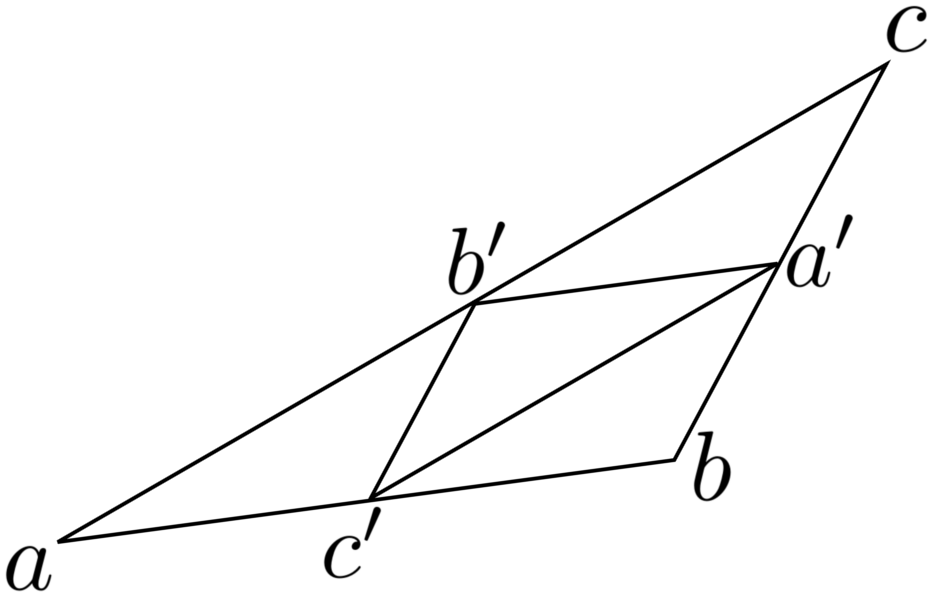
\includegraphics[width=0.3\textwidth]{12.png}
  \end{center}
\end{wrapfigure}

Dado um tir\^{a}ngulo $\Delta=(  a,b,c)  \in%
%TCIMACRO{\U{2102} }%
%BeginExpansion
\mathbb{C}
%EndExpansion
^{3},$ 

sejam\\\\

$a^{\prime}=$ ponto médio de $\left[  b,c\right]  $

$b^{\prime}=$ ponto médio de $\left[  a,c\right]  $

$c^{\prime}=$ ponto médio de $\left[  a,b\right]  $\\\\

e consideremos os quatro

tri\^{a}ngulos resultantes:

$\Delta^{(  1)  }=(  a,c^{\prime},b^{\prime})  ,$
$\Delta^{(  2)  }=(  b,a^{\prime},c^{\prime})  ,$
$\Delta^{(  3)  }=(  c,b^{\prime},a^{\prime})  ,$
$\Delta^{(  4)  }=(  a^{\prime},b^{\prime},c^{\prime})
.$

Indicando a congruência com o símbolo $\equiv,$ é claro que

\ \ \ \ \ \ \ \ \ \ \ \ \ \ \ \ \ \ \ \ \ \ \ \ \ \ \ \ \ \ \ \ \ \ $\Delta
^{(  1)  }\equiv\Delta^{(  2)  }\equiv\Delta^{(
3)  }\equiv\Delta^{(  4)  }$

e que estes quatro tri\^{a}ngulos são semelhantes a $\Delta.$ Como
$\Delta^{(  1)  }$ se transforma

em $\Delta$ por uma homotetia de centro $a$ e razão $2,$ é imediato
verificar que

$diam(  \Delta)  =2$ $diam(  \Delta^{(  1)
})  $ \ donde

$diam(  \Delta^{(  1)  })  =diam(  \Delta^{(
2)  })  =diam(  \Delta^{(  3)  })
=diam(  \Delta^{(  4)  })  =%
%TCIMACRO{\QDABOVE{1pt}{diam(  \Delta)  }{2}}%
%BeginExpansion
\genfrac{}{}{1pt}{0}{diam(  \Delta)  }{2}%
%EndExpansion
$

\bigskip

Considerando as CSDF definidas pelos cinco tri\^{a}ngulos anteriores é claro

que valem as seguintes relações entre os comprimentos:

\ \ \ \ \ \ \ \ \ \ \ \ \ \ \ \ \ \ \ \ \ \ $\left\vert \partial
\Delta^{(  1)  }\right\vert =\left\vert \partial\Delta^{(
2)  }\right\vert =\left\vert \partial\Delta^{(  3)
}\right\vert =\left\vert \partial\Delta^{(  4)  }\right\vert =%
%TCIMACRO{\QDABOVE{1pt}{1}{2}}%
%BeginExpansion
\genfrac{}{}{1pt}{0}{1}{2}%
%EndExpansion
\left\vert \partial\Delta\right\vert .$

\bigskip

\textbf{Observação 2} \ Seja $K$ um subconjunto não vazio de $%
%TCIMACRO{\U{2102} }%
%BeginExpansion
\mathbb{C}
%EndExpansion
,$ então são equiva-

lentes as afirmações seguintes:

(i) \ \ $K$ é compacto;

(ii) \ Para cada família $(  F_{\lambda})  _{\lambda\in
\Lambda}$ de conjuntos fechados em $\ K$ \ tal que

$\ \ \ \ \ \ \ \ \ \ \ \ \ \ \ \ \ \ \ \ \ \ \ \ \ \ \ \ \ \ \ \ \underset
{\lambda\in\Lambda}{\bigcap}F_{\lambda}=\varnothing,$

existe uma subfamília finita não vazia $\ (  F_{\lambda})
_{\in\Lambda_{0}}$ de $\ (  F_{\lambda})  _{\lambda\in\Lambda}$
\ tal \ que

$\ \ \ \ \ \ \ \ \ \ \ \ \ \ \ \ \ \ \ \ \ \ \ \ \ \ \ \ \ \underset
{\lambda\in\Lambda_{0}}{\bigcap}F_{\lambda}=\varnothing.$

\bigskip

\textbf{Oservação 3} \ Sejam $K$ um subconjunto compacto não vazio
de $%
%TCIMACRO{\U{2102} }%
%BeginExpansion
\mathbb{C}
%EndExpansion
,$ $(  F_{m})  _{m\geq1}$

uma sequência de conjuntos fechados \underline{não vazios} \ tais que:

(1) \ \ $K\supset F_{1}\supset F_{2}\supset$ \ $\ldots$ $\supset F_{m}\supset
F_{m+1}\supset$ $\ldots$

(2) \ $\underset{m\rightarrow\infty}{\lim}\left[  diam(  F_{m})
\right]  =0$

\bigskip Então, existe $z\in K$ \ tal que $\underset{m\geq1}{\bigcap}%
F_{m}=\left\{  z\right\}  .$

\bigskip

De fato, \ como para cada $m\in%
%TCIMACRO{\U{2115} }%
%BeginExpansion
\mathbb{N}
%EndExpansion
$ o conjunto $F_{m}$ é fechado resulta que $F_{m}$ \ é

fechado em $K,$ logo se fosse $\underset{m\geq1}{\bigcap}F_{m}=\varnothing,$
pela Obs. 2 precedente existiria

uma parte \ finita $J$ de $%
%TCIMACRO{\U{2115} }%
%BeginExpansion
\mathbb{N}
%EndExpansion
$ tal que

\ \ \ \ \ \ \ \ \ \ \ \ \ \ \ \ \ \ \ \ \ \ \ \ \ \ \ \ \ \ \ \ \ \ \ \ \ \ \ $\underset
{m\in J}{\bigcap}F_{m}=\varnothing$

o que é absurdo pois como $(  F_{m})  $ é decrescente,
é claro que

\ \ \ \ \ \ \ \ \ \ \ \ \ \ \ \ \ \ \ \ \ \ \ \ \ \ \ \ \ \ \ \ \ \ \ \ \ $\underset
{m\in J}{\bigcap}F_{m}=F_{\nu}\neq\varnothing$

onde $\nu=\max$ $J.$ Em consequência temos \textsc{I} : =$\underset
{m\geq1}{\bigcap}F_{m}\neq\varnothing.$ Mostremos que

\textsc{I} contém apenas um ponto. Suponhamos por absurdo que existem
$z,w\in$ \textsc{I}

tais que $z\neq w,$ então

\ \ \ \ \ \ \ \ \ \ \ \ \ \ \ \ \ \ \ \ \ \ \ \ \ \ \ \ \ \ \ \ $\left\{
z,w\right\}  \subset$ \textsc{I}$\subset F_{m}$ \ \ $\forall$ \ $m\in%
%TCIMACRO{\U{2115} }%
%BeginExpansion
\mathbb{N}
%EndExpansion
,$

donde, para cada $m\in%
%TCIMACRO{\U{2115} }%
%BeginExpansion
\mathbb{N}
%EndExpansion
$ resultaria

\ \ \ \ \ \ \ \ \ \ \ \ \ \ \ \ \ \ \ \ \ \ \ \ \ \ \ \ \ \ $diam(
F_{m})  \geq\left\vert z-w\right\vert >0$ \ \ $\forall$ \ $m\geq1$

o que é absurdo pois

\ \ \ \ \ \ \ \ \ \ \ \ \ \ \ \ \ \ \ \ \ $0=\underset{m\rightarrow\infty
}{\lim}\left[  diam(  F_{m})  \right]  \geq\left\vert
z-w\right\vert >0$

Resulta então que \textsc{I} tem apenas um elemento, isto é, existe
$z\in K$ \ tal que

\textsc{I} =$\left\{  z\right\}  \subset F_{m}\subset K$ \ \ $\forall$ \ $m\in%
%TCIMACRO{\U{2115} }%
%BeginExpansion
\mathbb{N}
%EndExpansion
.$

\bigskip

\textbf{Prova do Lema 5.6 \ }Sejam

\ \ \ \ \ \ \ \ \ \ \ \ \ \ \ \ \ \ \ \ \ \ \ \ \ \ \ \ \ \ \ \ \ $\Delta
=(  a,b,c)  $ \ e \ $J \defeq %
%TCIMACRO{\dint _{\partial\Delta}}%
%BeginExpansion
{\displaystyle\int_{\partial\Delta}}
%EndExpansion
f(  z)  dz$

\bigskip

\textbf{Caso 1: \ }$p\notin\Delta.$ \ Sejam $a^{\prime},b^{\prime}$ e
$c^{\prime}$ os pontos médios de $\left[  b,c\right]  ,\left[  a,c\right]
$ e $\left[  a,b\right]  $

respectivamente e consideremos os tri\^{a}ngulos da Obs. 1 precedente

$\Delta^{(  1)  }=(  a,c^{\prime},b^{\prime})  $ \ ,
\ $\Delta^{(  2)  }=(  b,a^{\prime},c^{\prime})  $ \ ,
\ $\Delta^{(  3)  }=(  c,b^{\prime},a^{\prime})  $ \ \ e
\ $\Delta^{(  4)  }=(  a^{\prime},b^{\prime},c^{\prime
})  .$

É imediato verificar que

\ \ \ \ \ \ \ \ \ \ \ \ \ \ \ \ \ \ \ \ \ \ \ \ \ \ \ \ \ \ \ \ \ \ $J=\underset
{j=1}{\overset{4}{%
%TCIMACRO{\dsum }%
%BeginExpansion
{\displaystyle\sum}
%EndExpansion
}}\underset{\partial\Delta^{(  j)  }}{%
%TCIMACRO{\dint }%
%BeginExpansion
{\displaystyle\int}
%EndExpansion
}f(  z)  dz$


\begin{wrapfigure}[1]{r}{0.35\textwidth}
  \begin{center}
    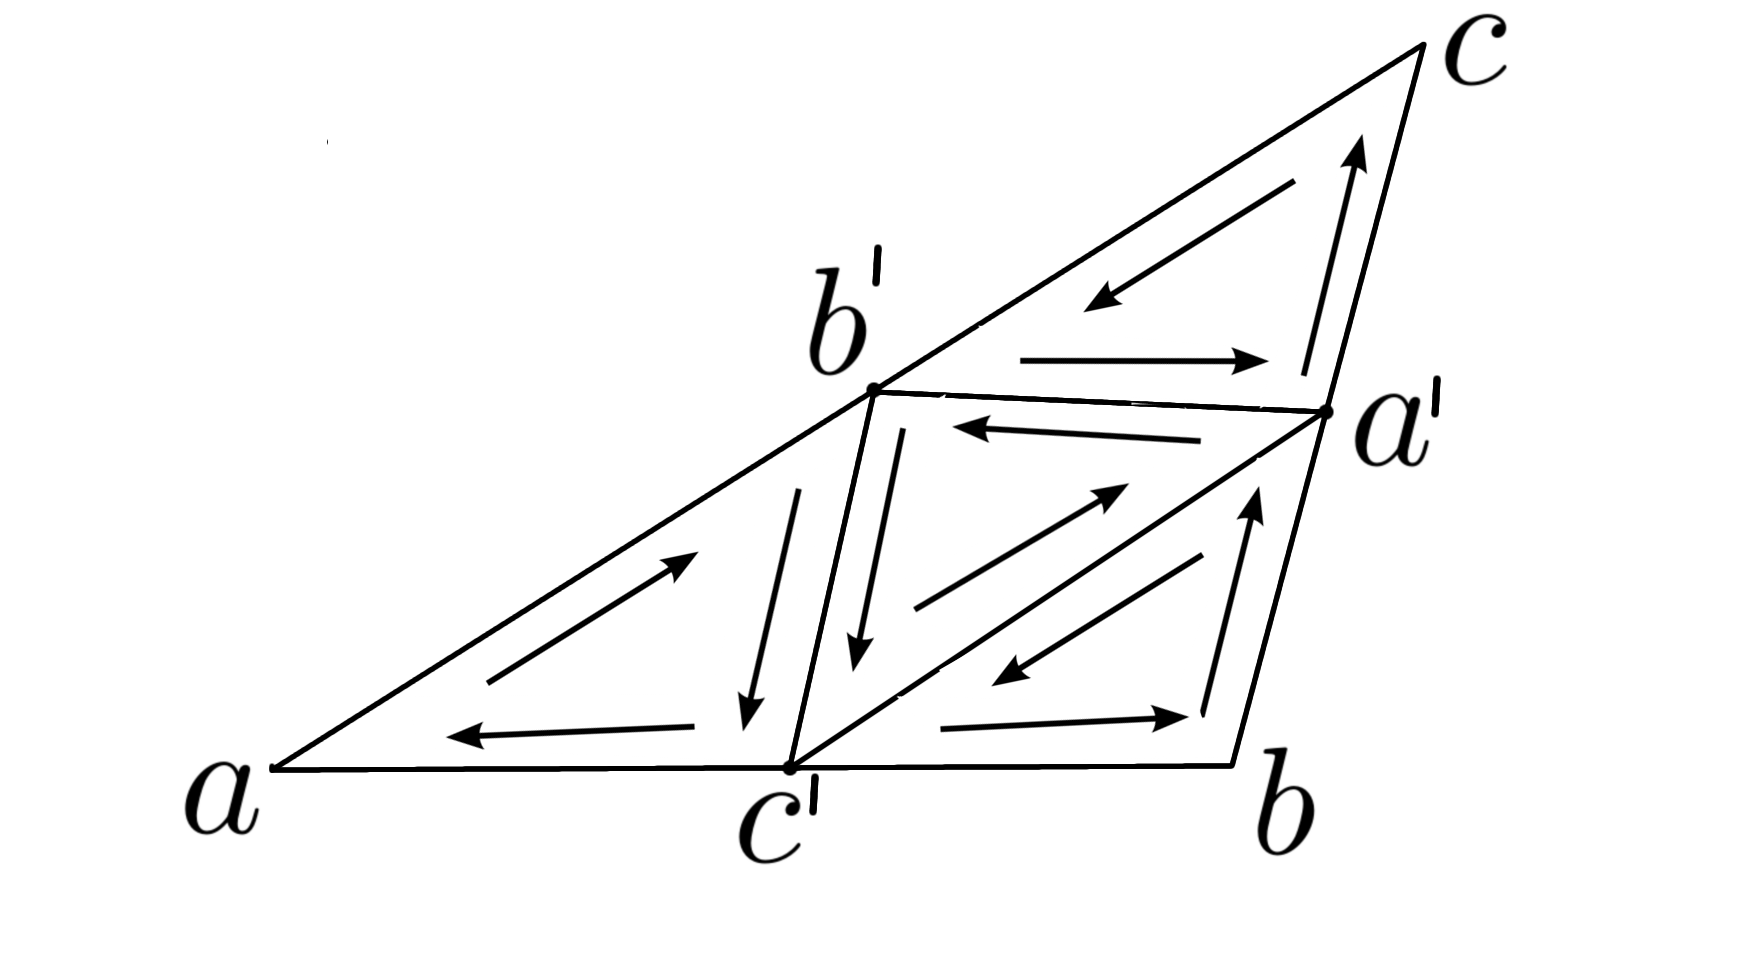
\includegraphics[width=0.35\textwidth]{14-3.png}
  \end{center}
\end{wrapfigure}

e portanto


\ \ \ \ \ \ \ \ \ \ \ \ \ \ \ \ \ \ \ \ \ $\left\vert J\right\vert
\leq\underset{j=1}{\overset{4}{%
%TCIMACRO{\dsum }%
%BeginExpansion
{\displaystyle\sum}
%EndExpansion
}}\left\vert \underset{\partial\Delta^{(  j)  }}{%
%TCIMACRO{\dint }%
%BeginExpansion
{\displaystyle\int}
%EndExpansion
}f(  z)  dz\right\vert $

o que mostra que, pelo menos um dos quatro 

somandos do segundo membro da desi-

gualdade acima é $\geq$ \ que $\left\vert J/4\right\vert . $ Seja $\Delta_{1}$ 

o tri\^{a}ngulo correspondente ao somando em questão, isto é, tal que

\ \ \ \ \ \ \ \ \ \ \ \ \ \ \ \ \ \ \ \ \ \ \ \ \ \ \ \ \ \ \ $\left\vert
\underset{\partial\Delta_{1}}{%
%TCIMACRO{\dint }%
%BeginExpansion
{\displaystyle\int}
%EndExpansion
}f(  z)  dz\right\vert \geq\left\vert J/4\right\vert $

Pela Obs. 1 precedente \ temos:

\ \ \ \ \ \ \ \ \ \ \ \ \ \ \ \ \ \ \ \ \ \ \ \ $diam(  \Delta
_{1})  =%
%TCIMACRO{\QDABOVE{1pt}{1}{2}}%
%BeginExpansion
\genfrac{}{}{1pt}{0}{1}{2}%
%EndExpansion
$ $diam(  \Delta)  $ \ \ \ e \ \ \ $\left\vert \partial\Delta
_{1}\right\vert =%
%TCIMACRO{\QDABOVE{1pt}{1}{2}}%
%BeginExpansion
\genfrac{}{}{1pt}{0}{1}{2}%
%EndExpansion
\left\vert \partial\Delta\right\vert $

Procedendo com o tri\^{a}ngulo $\Delta_{1}$ da mesma forma \ que com $\Delta,$
obtemos um

novo tri\^{a}ngulo $\Delta_{2}$ tal que

\ \ \ \ \ \ \ \ \ \ \ \ \ \ \ \ \ \ \ \ \ \ \ \ \ \ \ \ $\left\vert
\underset{\partial\Delta_{2}}{%
%TCIMACRO{\dint }%
%BeginExpansion
{\displaystyle\int}
%EndExpansion
}f(  z)  dz\right\vert \geq\left\vert J/4^{2}\right\vert $ \ ,

\ \ $diam(  \Delta_{2})  =%
%TCIMACRO{\QDABOVE{1pt}{1}{2}}%
%BeginExpansion
\genfrac{}{}{1pt}{0}{1}{2}%
%EndExpansion
$ $diam(  \Delta_{1})  =%
%TCIMACRO{\QDABOVE{1pt}{1}{2^{2}}}%
%BeginExpansion
\genfrac{}{}{1pt}{0}{1}{2^{2}}%
%EndExpansion
diam(  \Delta)  $ \ e \ \ $\left\vert \partial\Delta_{2}\right\vert
=%
%TCIMACRO{\QDABOVE{1pt}{1}{2}}%
%BeginExpansion
\genfrac{}{}{1pt}{0}{1}{2}%
%EndExpansion
\left\vert \partial\Delta_{1}\right\vert =%
%TCIMACRO{\QDABOVE{1pt}{1}{2^{2}}}%
%BeginExpansion
\genfrac{}{}{1pt}{0}{1}{2^{2}}%
%EndExpansion
\left\vert \partial\Delta\right\vert $ $.$

Prosseguindo desta forma construímos por indução uma
sequência de

tri\^{a}ngulos $(  \Delta_{m})  _{m\geq1}$ tal que para cada
\ $m\geq1$ temos

\ \ \ \ \ \ \ \ \ \ \ \ \ \ \ \ \ \ \ \ \ \ \ \ \ \ \ $\left\vert
\underset{\partial\Delta_{m}}{%
%TCIMACRO{\dint }%
%BeginExpansion
{\displaystyle\int}
%EndExpansion
}f(  z)  dz\right\vert \geq\left\vert J/4^{m}\right\vert $ ,

$diam(  \Delta_{m})  =%
%TCIMACRO{\QDABOVE{1pt}{1}{2^{m}}}%
%BeginExpansion
\genfrac{}{}{1pt}{0}{1}{2^{m}}%
%EndExpansion
$ $diam(  \Delta)  $ \ \ e \ \ \ $\left\vert \partial\Delta
_{m}\right\vert =%
%TCIMACRO{\QDABOVE{1pt}{1}{2^{m}}}%
%BeginExpansion
\genfrac{}{}{1pt}{0}{1}{2^{m}}%
%EndExpansion
\left\vert \partial\Delta\right\vert .$

\bigskip

Da desigualdade anterior resulta então

\bigskip

$(  5.6.1)  $ \ \ \ \ \ \ \ \ \ \ \ \ \ \ $\left\vert J\right\vert
\leq4^{m}\left\vert \underset{\partial\Delta_{m}}{%
%TCIMACRO{\dint }%
%BeginExpansion
{\displaystyle\int}
%EndExpansion
}f(  z)  dz\right\vert $ \ $,$ \ \ \ \ $\forall$ \ $m\geq1$

\bigskip

Observamos a seguir que $\Delta_{m}$ é fechado para cada $m\geq1,$ que
$\Delta\supset\Delta_{1}\supset$

$\Delta_{2}\supset$ $\cdots$ $\supset\Delta_{m}\supset\Delta_{m+1}%
\supset\cdots$ \ e que

\ \ \ \ \ \ \ \ \ \ \ \ \ \ \ \ \ \ \ \ \ \ $\underset{m\rightarrow\infty
}{\lim}\left[  diam(  \Delta_{m})  \right]  =diam(
\Delta)  \underset{m\rightarrow\infty}{\lim}%
%TCIMACRO{\QDABOVE{1pt}{1}{2^{m}}}%
%BeginExpansion
\genfrac{}{}{1pt}{0}{1}{2^{m}}%
%EndExpansion
=0$

\bigskip

Pela Obs. 3 anterior , existe $z_{0}\in\Delta$ tal que

\ \ \ \ \ \ \ \ \ \ \ \ \ \ \ \ \ \ \ \ \ \ \ \ \ $\underset{m\geq1}{%
%TCIMACRO{\dbigcap }%
%BeginExpansion
{\displaystyle\bigcap}
%EndExpansion
}\Delta_{m}=\left\{  z_{0}\right\}  $

Como $z_{0}\in\Delta$ e $p\notin\Delta$ resulta $p\neq z_{0},$ logo $f$ é
$%
%TCIMACRO{\U{2102} }%
%BeginExpansion
\mathbb{C}
%EndExpansion
$-derivável em $z_{0},$ donde pelo

Lema 1.3 existe $r>0$ tal que $D_{r}(  z_{0})  \subset\Omega$ e
existe $\varphi:D_{r}(  z_{0})  \rightarrow%
%TCIMACRO{\U{2102} }%
%BeginExpansion
\mathbb{C}
%EndExpansion
$ contínua

em $z_{0}$ tal que $\varphi(  z_{0})  =0,$ de modo que

\ \ \ \ \ \ \ \ \ $f(  z)  -f(  z_{0})  -f^{\prime
}(  z_{0})  (  z-z_{0})  =(  z-z_{0})
\varphi(  z)  $ \ \ $\forall$ \ $z\in D_{r}(  z_{0})  .$

\bigskip

Fixemos $\varepsilon>0$ arbitrário. Pela continuidade de $\varphi$ em
$z_{0\text{ }}$ e por ser $\varphi(  z_{0})  =0,$

existe $\delta\in\left]  0,r\right[  $ tal que $\left\vert \varphi(
z)  \right\vert \leq\varepsilon$ sempre que $z\in D_{\delta}(
z_{0})  $ e em consequência:

\bigskip

$(  5.6.2)  $ \ \ \ $\left\vert f(  z)  -f(
z_{0})  -f^{\prime}(  z_{0})  (  z-z_{0})
\right\vert \leq\varepsilon\left\vert z-z_{0}\right\vert $ \ \ $\forall$
\ $z\in D_{\delta}(  z_{0})  $

\bigskip

Por outro lado, como $z_{0}\in\Delta_{m}$ $\ \forall$ \ $m\in%
%TCIMACRO{\U{2115} }%
%BeginExpansion
\mathbb{N}
%EndExpansion
$ e $\underset{m\rightarrow\infty}{\lim}\left[  diam(  \Delta_{m})
\right]  =0,$ existe

$\nu\in%
%TCIMACRO{\U{2115} }%
%BeginExpansion
\mathbb{N}
%EndExpansion
$ \ tal que $\Delta_{\nu}\subset D_{\delta}(  z_{0})  $ e é
claro que:


% IMAGEM 13
\begin{wrapfigure}[1]{r}{0.3\textwidth}
  \begin{center}
    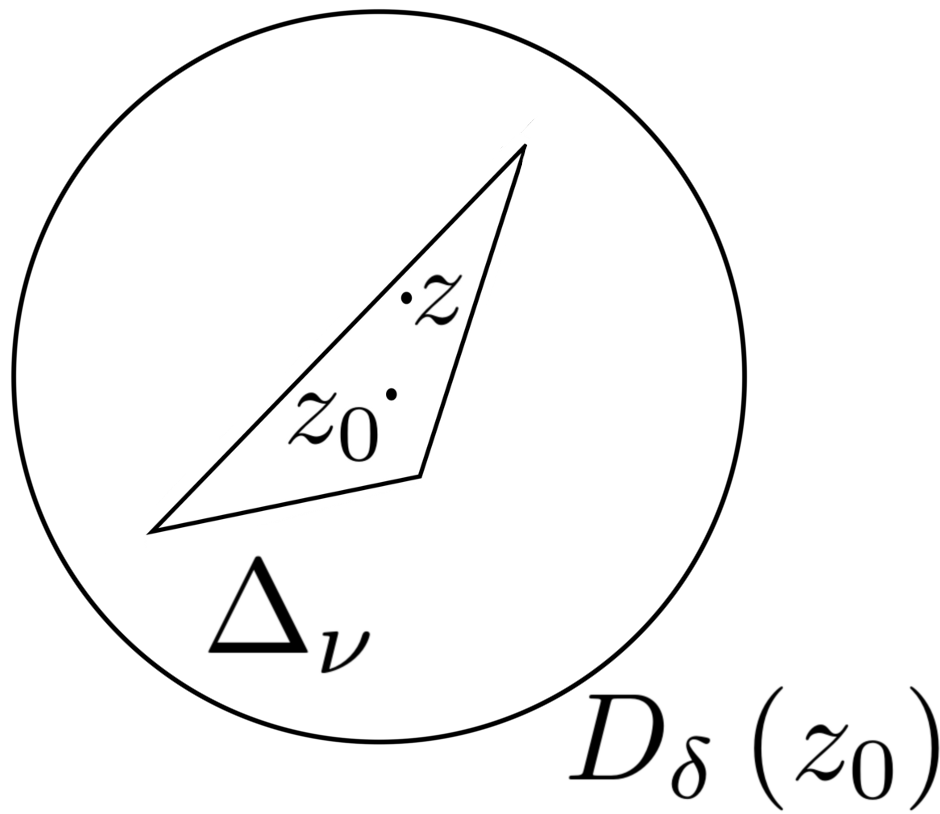
\includegraphics[width=0.3\textwidth]{13.png}
  \end{center}
\end{wrapfigure}

\bigskip

$(  5.6.3)  $ \ \ \ \ $\left\vert z-z_{0}\right\vert \leq\left\vert
\partial\Delta_{v}\right\vert =%
%TCIMACRO{\QDABOVE{1pt}{1}{2^{\nu}}}%
%BeginExpansion
\genfrac{}{}{1pt}{0}{1}{2^{\nu}}%
%EndExpansion
\left\vert \partial\Delta\right\vert ,$ \ \ $\forall$ \ $z\in\Delta_{\nu}$

\bigskip

Ora, pelo Corol. 5.5 temos:

\bigskip

$\underset{\partial\Delta_{\nu}}{%
%TCIMACRO{\dint }%
%BeginExpansion
{\displaystyle\int}
%EndExpansion
}f(  z_{0})  dz=0$ \ \ \ \ e \ \ \ \ \ $\underset{\partial
\Delta_{\nu}}{%
%TCIMACRO{\dint }%
%BeginExpansion
{\displaystyle\int}
%EndExpansion
}f^{\prime}(  z_{0})  (  z-z_{0})  dz=0$

\bigskip

o que implica

\bigskip

$(  5.6.4)  $ \ \ \ \ \ \ $\underset{\partial\Delta_{\nu}}{%
%TCIMACRO{\dint }%
%BeginExpansion
{\displaystyle\int}
%EndExpansion
}f(  z)  dz=\underset{\partial\Delta_{\nu}}{%
%TCIMACRO{\dint }%
%BeginExpansion
{\displaystyle\int}
%EndExpansion
}\left[  f(  z)  -f(  z_{0})  -f^{\prime}(
z_{0})  (  z-z_{0})  \right]  dz$

\bigskip

De $(5.6.1), (5.6.2), (5.6.3)$ e $(5.6.4)$ resulta então:

\bigskip

$\ \ \ \ \ \left\vert J\right\vert \leq4^{\nu}\left\vert \underset
{\partial\Delta_{\nu}}{{\displaystyle\int} f(z)} dz\right\vert = 4^{\nu}\left\vert \underset{\partial
\Delta_{\nu}}{{\displaystyle\int}}[ f(z) - f(z_{0}) - f^{\prime}(z_{0})  (z-z_{0}) ]  dz \right\vert \leq$

\bigskip

$\leq4^{\nu}\!\underset{\partial\Delta_{\nu}}{{\displaystyle\int}} \left\vert f(z) - f(z_{0}) - f^{\prime}(z_{0})  (z-z_{0})  \right\vert \left\vert dz\right\vert
 \leq  4^{\nu}\!\underset{\partial\Delta_{\nu}}{{\displaystyle\int}}\varepsilon\left\vert z-z_{0}\right\vert \left\vert dz\right\vert \leq$

\bigskip

$\leq4^{\nu}\varepsilon\genfrac{}{}{1pt}{0}{1}{2^{\nu}}\left\vert \partial\Delta\right\vert \underset{\partial\Delta_{\nu}}{{\displaystyle\int}}\left\vert dz\right\vert 
=4^{\nu}\varepsilon\genfrac{}{}{1pt}{0}{\left\vert \partial\Delta\right\vert }{2^{\nu}}\left\vert \partial\Delta_{\nu}\right\vert 
=4^{\nu}\varepsilon\genfrac{}{}{1pt}{0}{\left\vert \partial\Delta\right\vert }{2^{\nu}}\genfrac{}{}{1pt}{0}{\left\vert \partial\Delta\right\vert }{2^{\nu}}
\varepsilon\left\vert \partial\Delta\right\vert ^{2}$,

isto é,

\ \ \ \ \ \ \ \ \ \ \ \ \ \ \ \ \ \ \ \ \ \ \ \ \ \ \ \ \ $\left\vert
J\right\vert \leq\varepsilon\left\vert \partial\Delta\right\vert $

\bigskip


o que mostra que $J=0$ pois $\varepsilon$ era arbitrário.

\bigskip

\textbf{Caso 2: \ }$p$ é um vértice de $\Delta,$ por exemplo $p=a$. Se $a,b$ e $c$ são colineares

então é claro que $J=0,$ logo podemos supor que $a,b$ e $c$ não são colineares.


% IMAGEM 14
\begin{wrapfigure}[1]{r}{0.35\textwidth}
  \begin{center}
    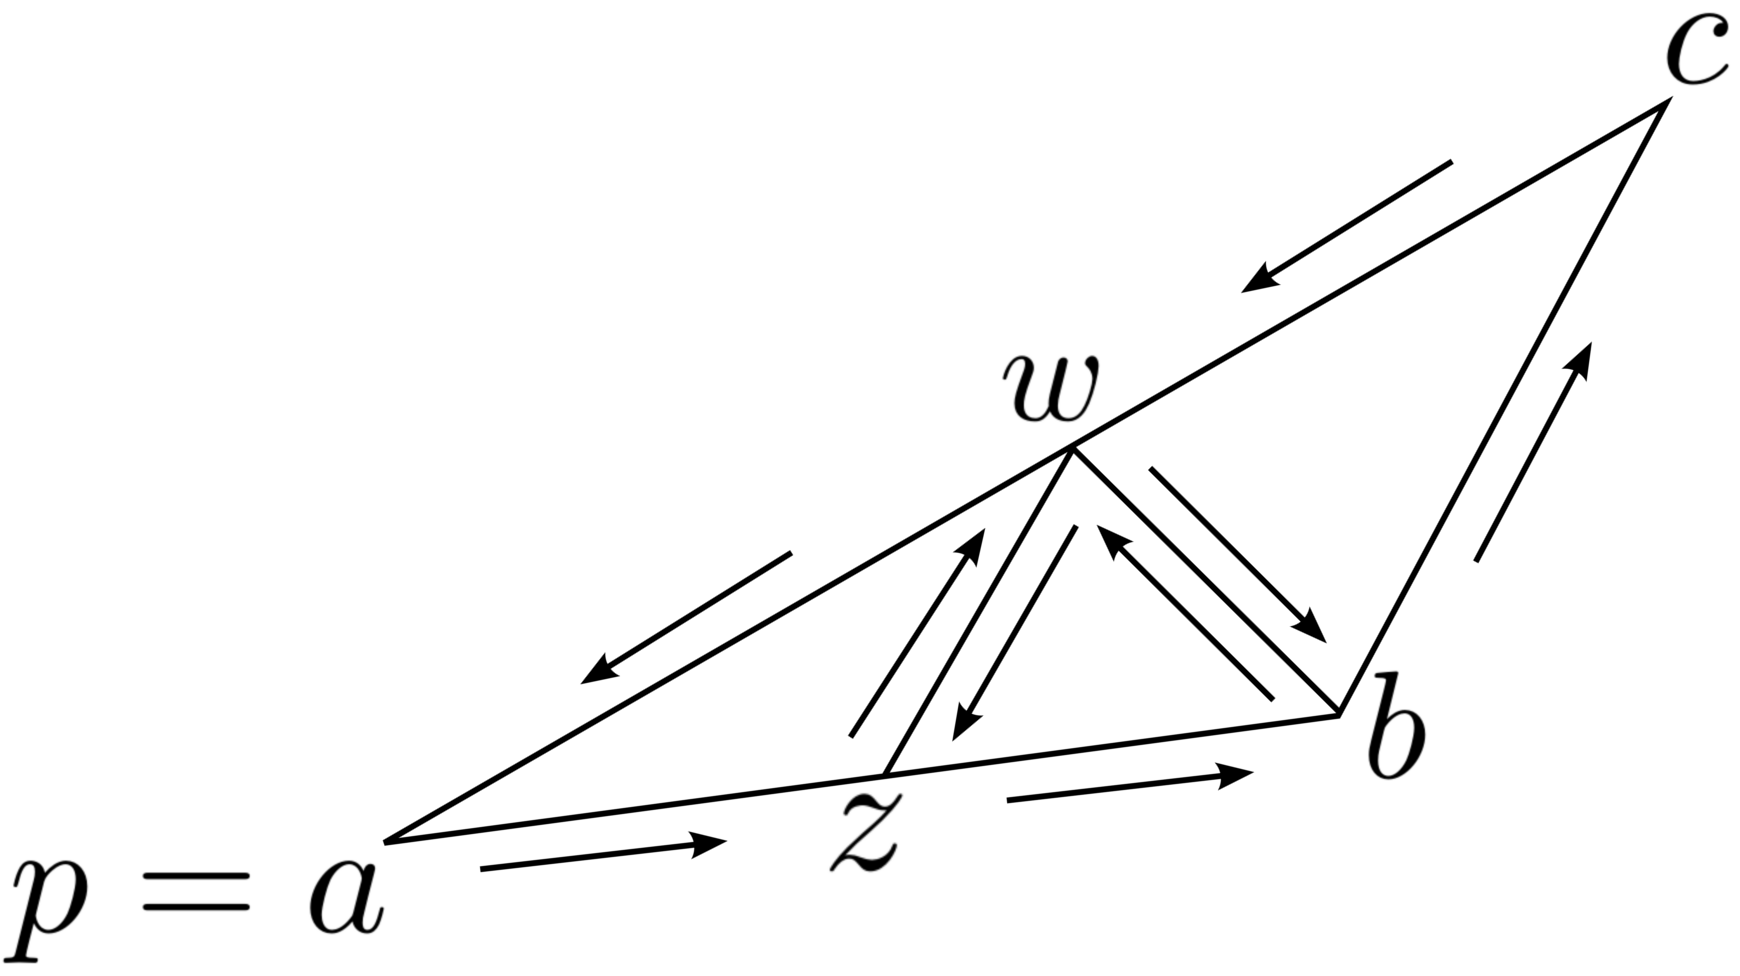
\includegraphics[width=0.35\textwidth]{14.png}
  \end{center}
\end{wrapfigure}



Sejam $z\in\left[  a,b\right]  $ e $w\in\left[  a,c\right]  $ pontos tais que

$z\neq a,b$ e $w\neq a,c$ e sejam $\Delta_{1}=(a,z,w)$,

$\Delta_{2}=(z,b,w)$ e $\Delta_{3}=(b,c,w)$.

Então é claro que\\

\ \ \ \ \ \ \ \ \ \ \ \  $J=\underset{j=1}{\overset{3}{{\displaystyle\sum}}}\underset{\partial\Delta_{j}}{{\displaystyle\int}}f$\\

Como $a,b$ e $c$ não são colineares, $p=a$ e $z$ e

$w$ não são vértices de $\Delta,$ resulta $p\notin\Delta_{2}$ 

e $p\notin\Delta_{3},$ logo pelo Caso 1 temos:\\

\ \ \ \ \ \ \ \ \ \ \ \ \ \ \ \ \ \ \ \ \ \ \ \ \ \ \ \ \ \ \ $\underset
{\partial\Delta_{2}}{%
%TCIMACRO{\dint }%
%BeginExpansion
{\displaystyle\int}
%EndExpansion
}f=\underset{\partial\Delta_{3}}{%
%TCIMACRO{\dint }%
%BeginExpansion
{\displaystyle\int}
%EndExpansion
}f=0$

donde

\bigskip

$(  5.6.5)  $ \ \ \ \ \ \ \ \ \ \ \ \ \ \ \ \ \ $J=\underset
{\partial\Delta_{1}}{%
%TCIMACRO{\dint }%
%BeginExpansion
{\displaystyle\int}
%EndExpansion
}f$

\bigskip

Como $\Delta$ é compacto e $f\in\mathcal{C}(  \Delta)  :$

\bigskip\ \ \ \ \ \ \ \ \ \ \ \ \ \ \ \ \ \ \ \ \ $\left\Vert f\right\Vert
_{\partial\Delta_{1}}\leq\left\Vert f\right\Vert _{\Delta_{1}}\leq\left\Vert
f\right\Vert _{\Delta}<+\infty$

\bigskip

e então de $(  5.6.5)  $ resulta

\ \ \ \ \ \ \ \ \ \ \ \ \ \ \ \ \ \ \ $\left\vert J\right\vert \leq
\underset{\partial\Delta_{1}}{%
%TCIMACRO{\dint }%
%BeginExpansion
{\displaystyle\int}
%EndExpansion
}\left\vert f(  z)  \right\vert \left\vert dz\right\vert
\leq\left\Vert f\right\Vert _{\Delta}\cdot\left\vert \partial\Delta
_{1}\right\vert $

\bigskip

o que prova que $J=0$ pois $\left\vert \partial\Delta_{1}\right\vert $ pode
ser feito arbitrariamente pequeno




a condição de tomar $z$ e $w$ suficientemente próximos


% IMAGEM 15 (que na verdade é  a 16)
\begin{wrapfigure}{r}{0.25\textwidth}
  \begin{center}
    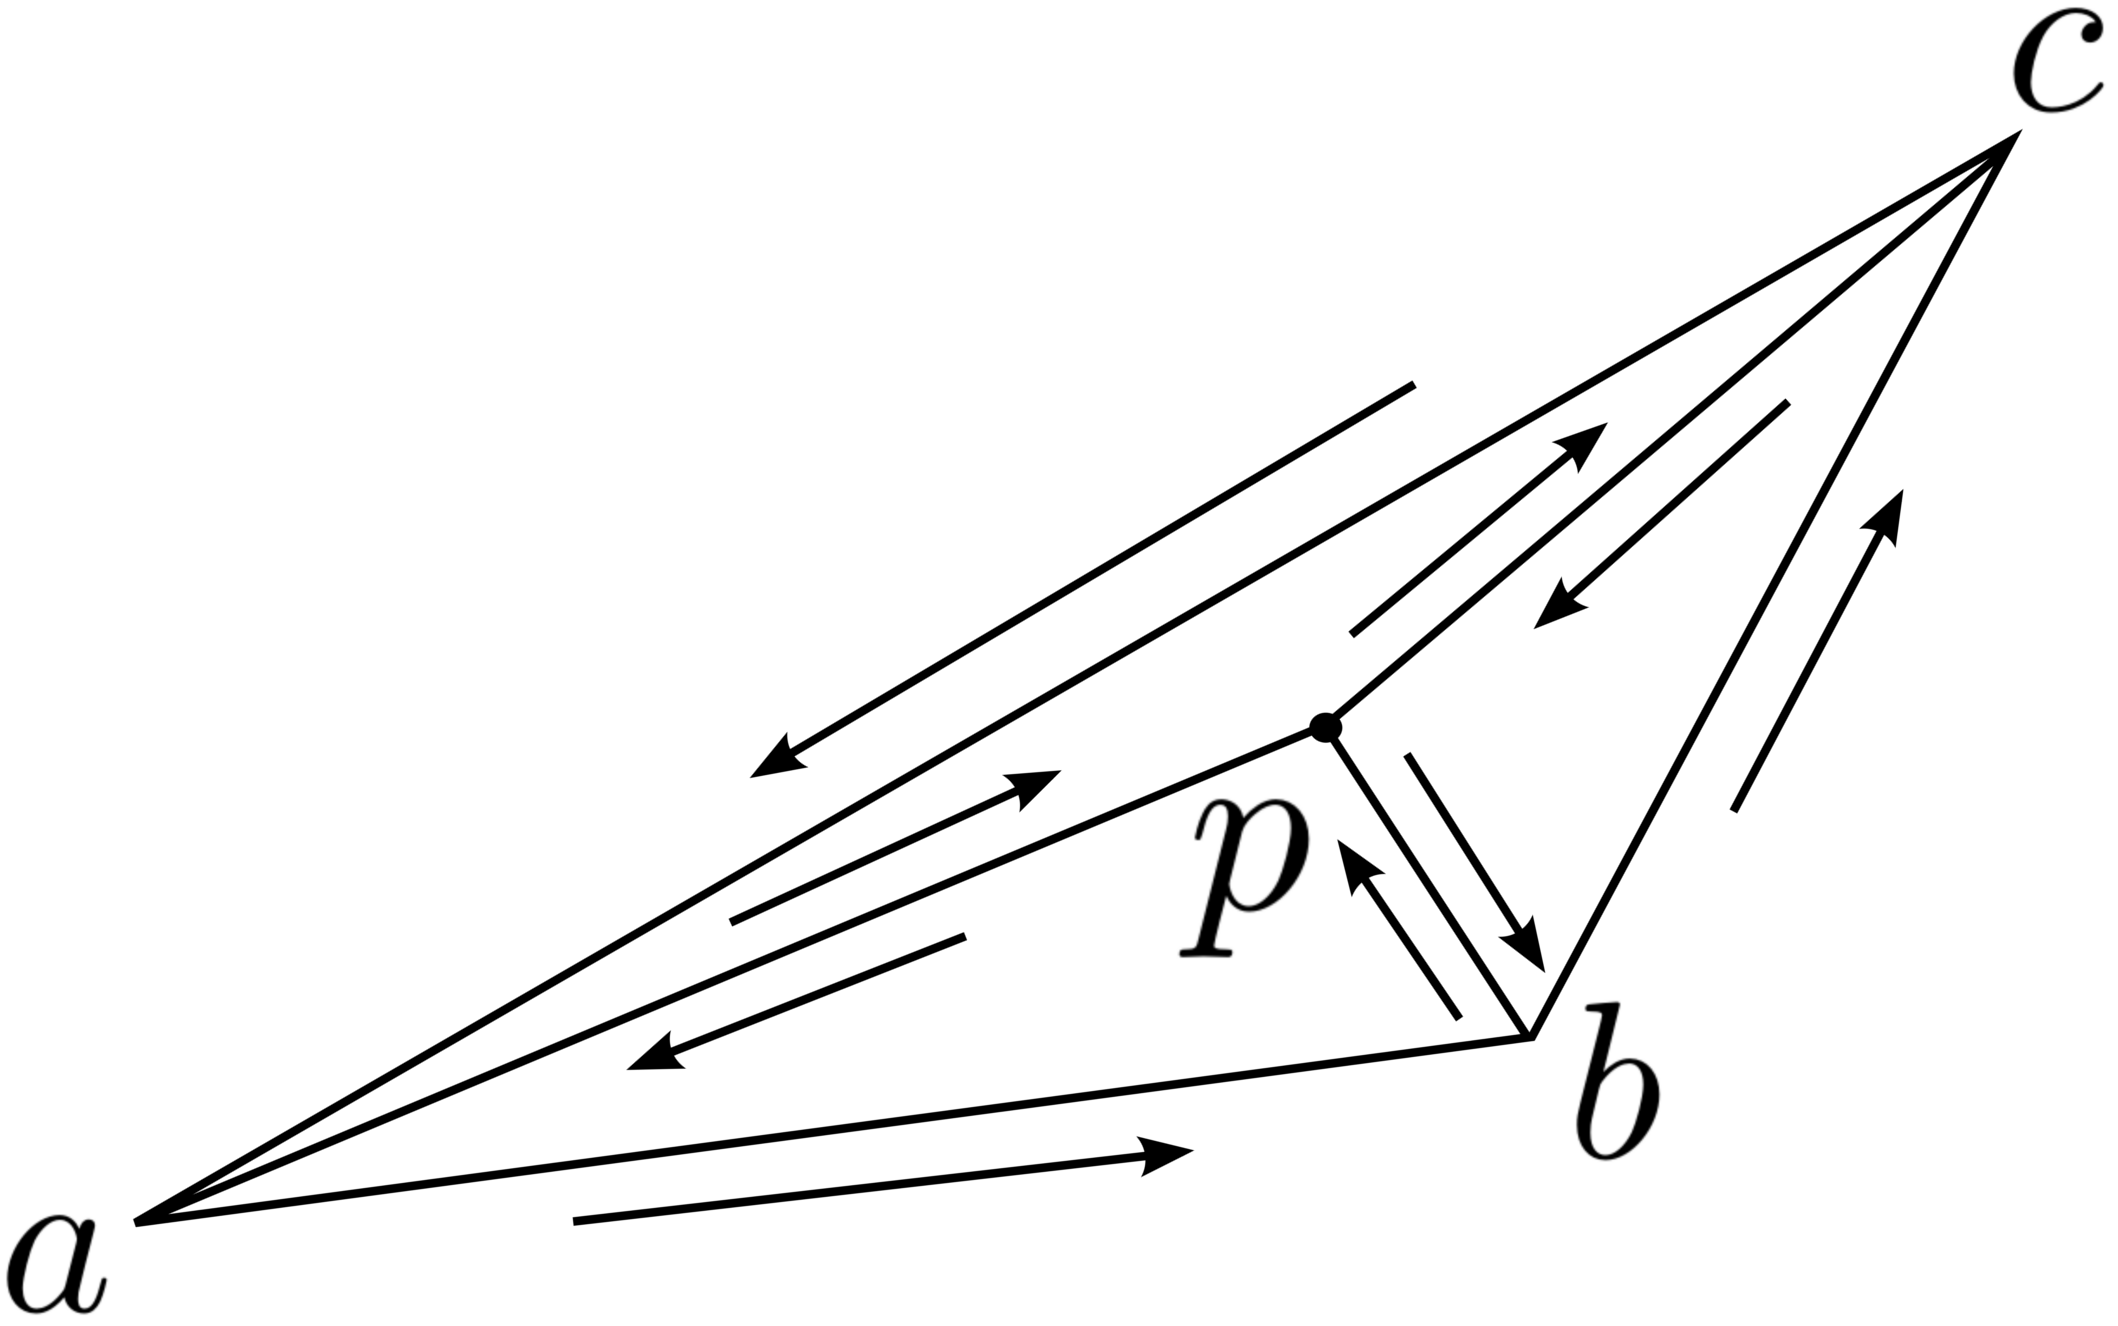
\includegraphics[width=0.25\textwidth]{16.png}
  \end{center}
\end{wrapfigure}


de $a.$\\



\textbf{Caso 3: \ }$p\in\Delta$ e $p$ não é vértice de $\Delta$

% IMAGEM 16 (que na verdade é a 15)
\begin{wrapfigure}{r}{0.25\textwidth}
  \begin{center}
    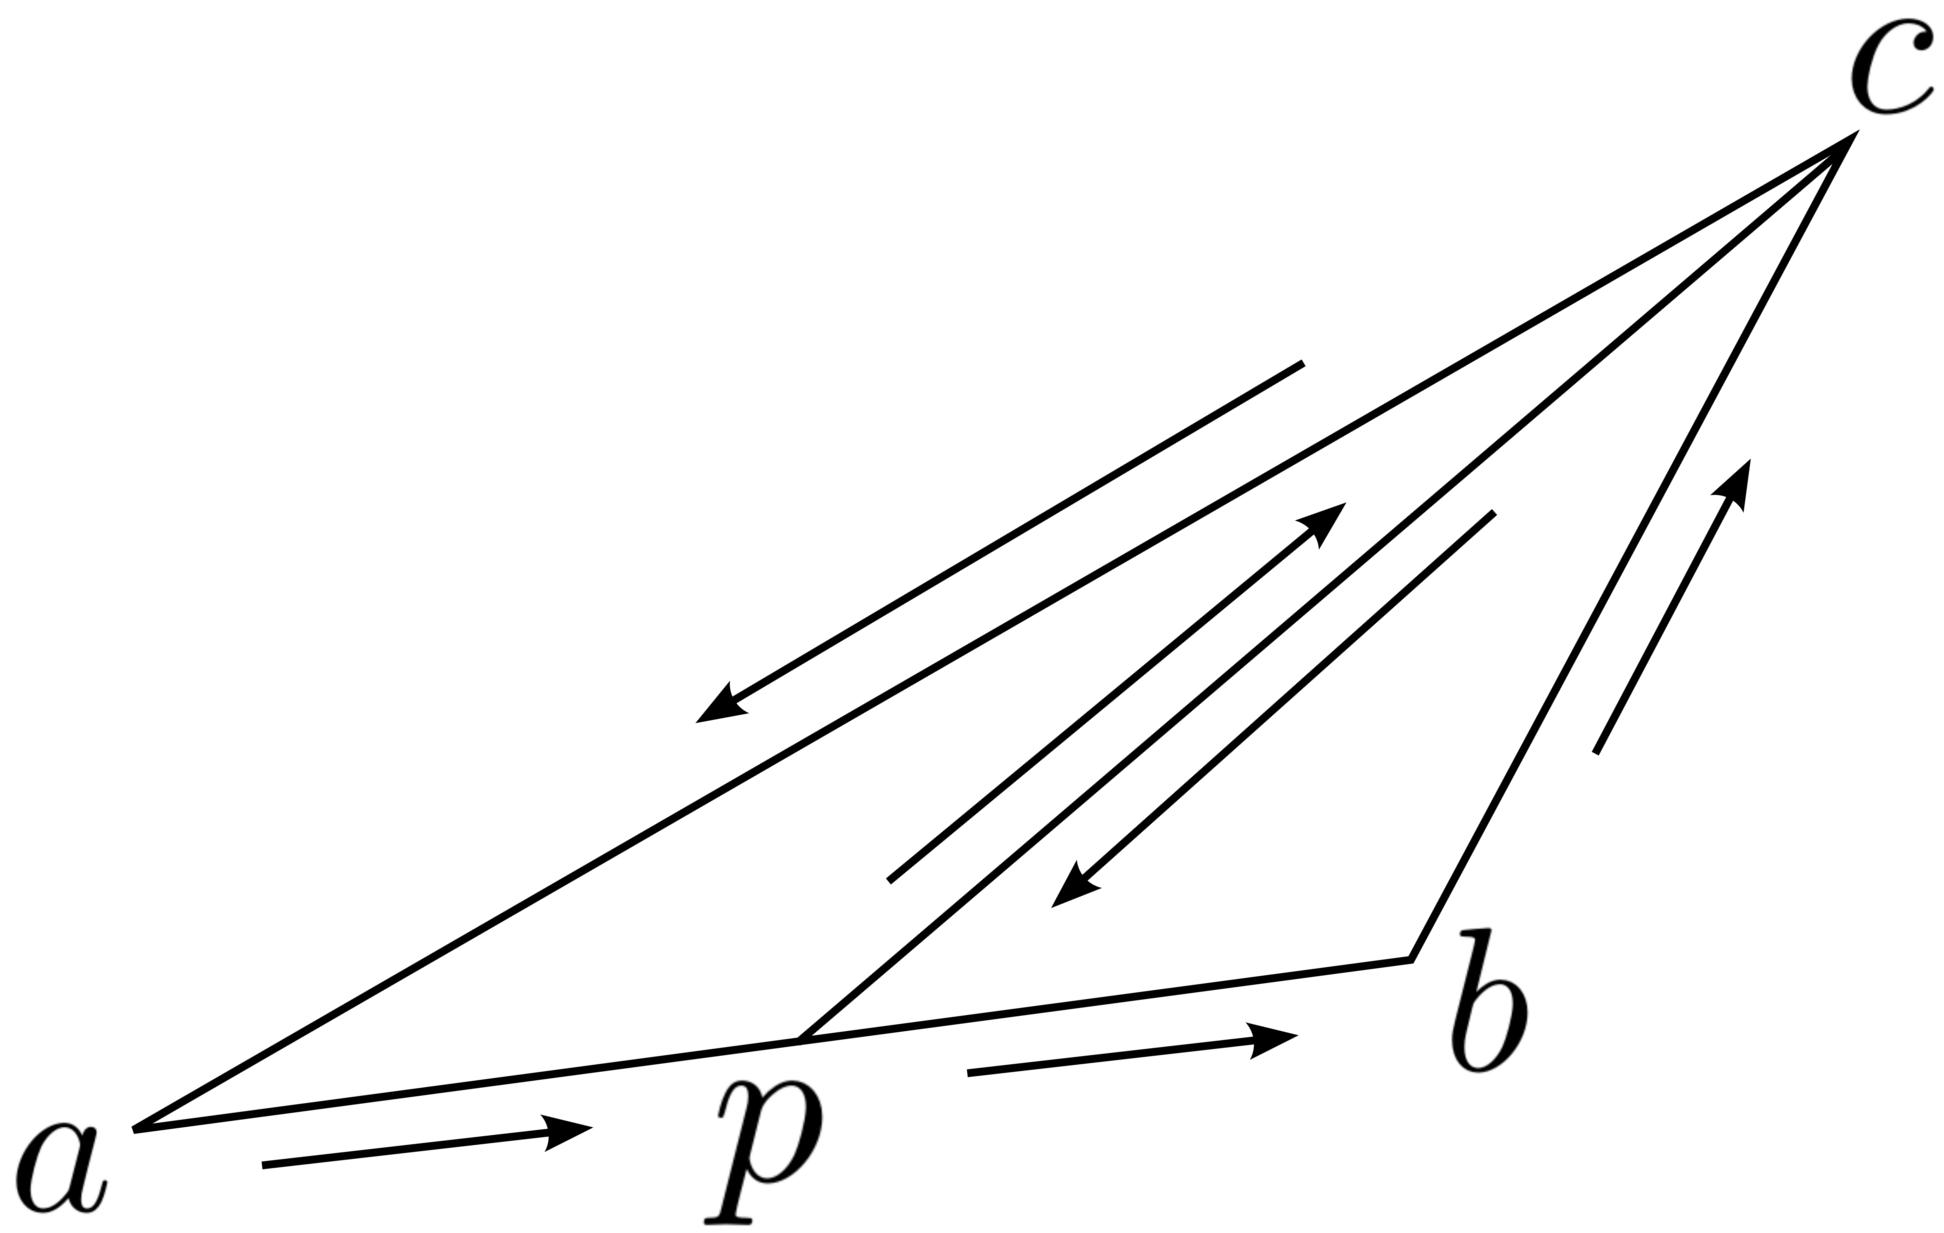
\includegraphics[width=0.25\textwidth]{15.png}
  \end{center}
\end{wrapfigure}

Como\\





$J=\underset{\partial(a,b,p)}{{\displaystyle\int}\text{ }f}+\underset{\partial( b,c,p)  }{{\displaystyle\int}\text{ }f}+\underset{\partial(  c,a,p)  }{{\displaystyle\int}\text{ }f}$\\\\


resulta $J=0$ pois cada uma das três integrais

ssé nula pelo Caso 2.\\

\bigskip

\textbf{Caso 4: \ }$p$ pertence a um lado de $\Delta$ sem ser

vértice de $\Delta$. Este caso se reduz imediatamente

ao Caso 2. \ $\square$\\\\\\

\textbf{\ Teorema 5.7 \ }(O teorema de Cauchy num aberto convexo)
\ \textit{Sejam }$\Omega$

\textit{um aberto convexo não vazio, }$p\in\Omega$ \textit{e }%
$f\in\mathcal{C}(  \Omega)  $ \textit{tal que }$f\in\mathcal{H(}%
\Omega\backslash\left\{  p\right\}  ).$

\textit{Então, existe }$F\in\mathcal{H}(  \Omega)  $
\textit{tal que }$F^{\prime}=f$ \textit{e em consequência}

\bigskip




$(  5.7.1)  $ \ \ \ \ \ \ \ \ $\underset{\gamma}{%
%TCIMACRO{\dint }%
%BeginExpansion
{\displaystyle\int}
%EndExpansion
}f(  z)  dz=0$ \ \ \ \ \ \ \ \ \textit{para cada CSDF }$\gamma$
\textit{em }$\Omega.$

\bigskip

\textbf{Prova \ }Fixemos\textbf{\ }$a\in\Omega.$ Como $\Omega$ é convexo, para

% IMAGEM 17
\begin{wrapfigure}{r}{0.2\textwidth}
  \begin{center}
    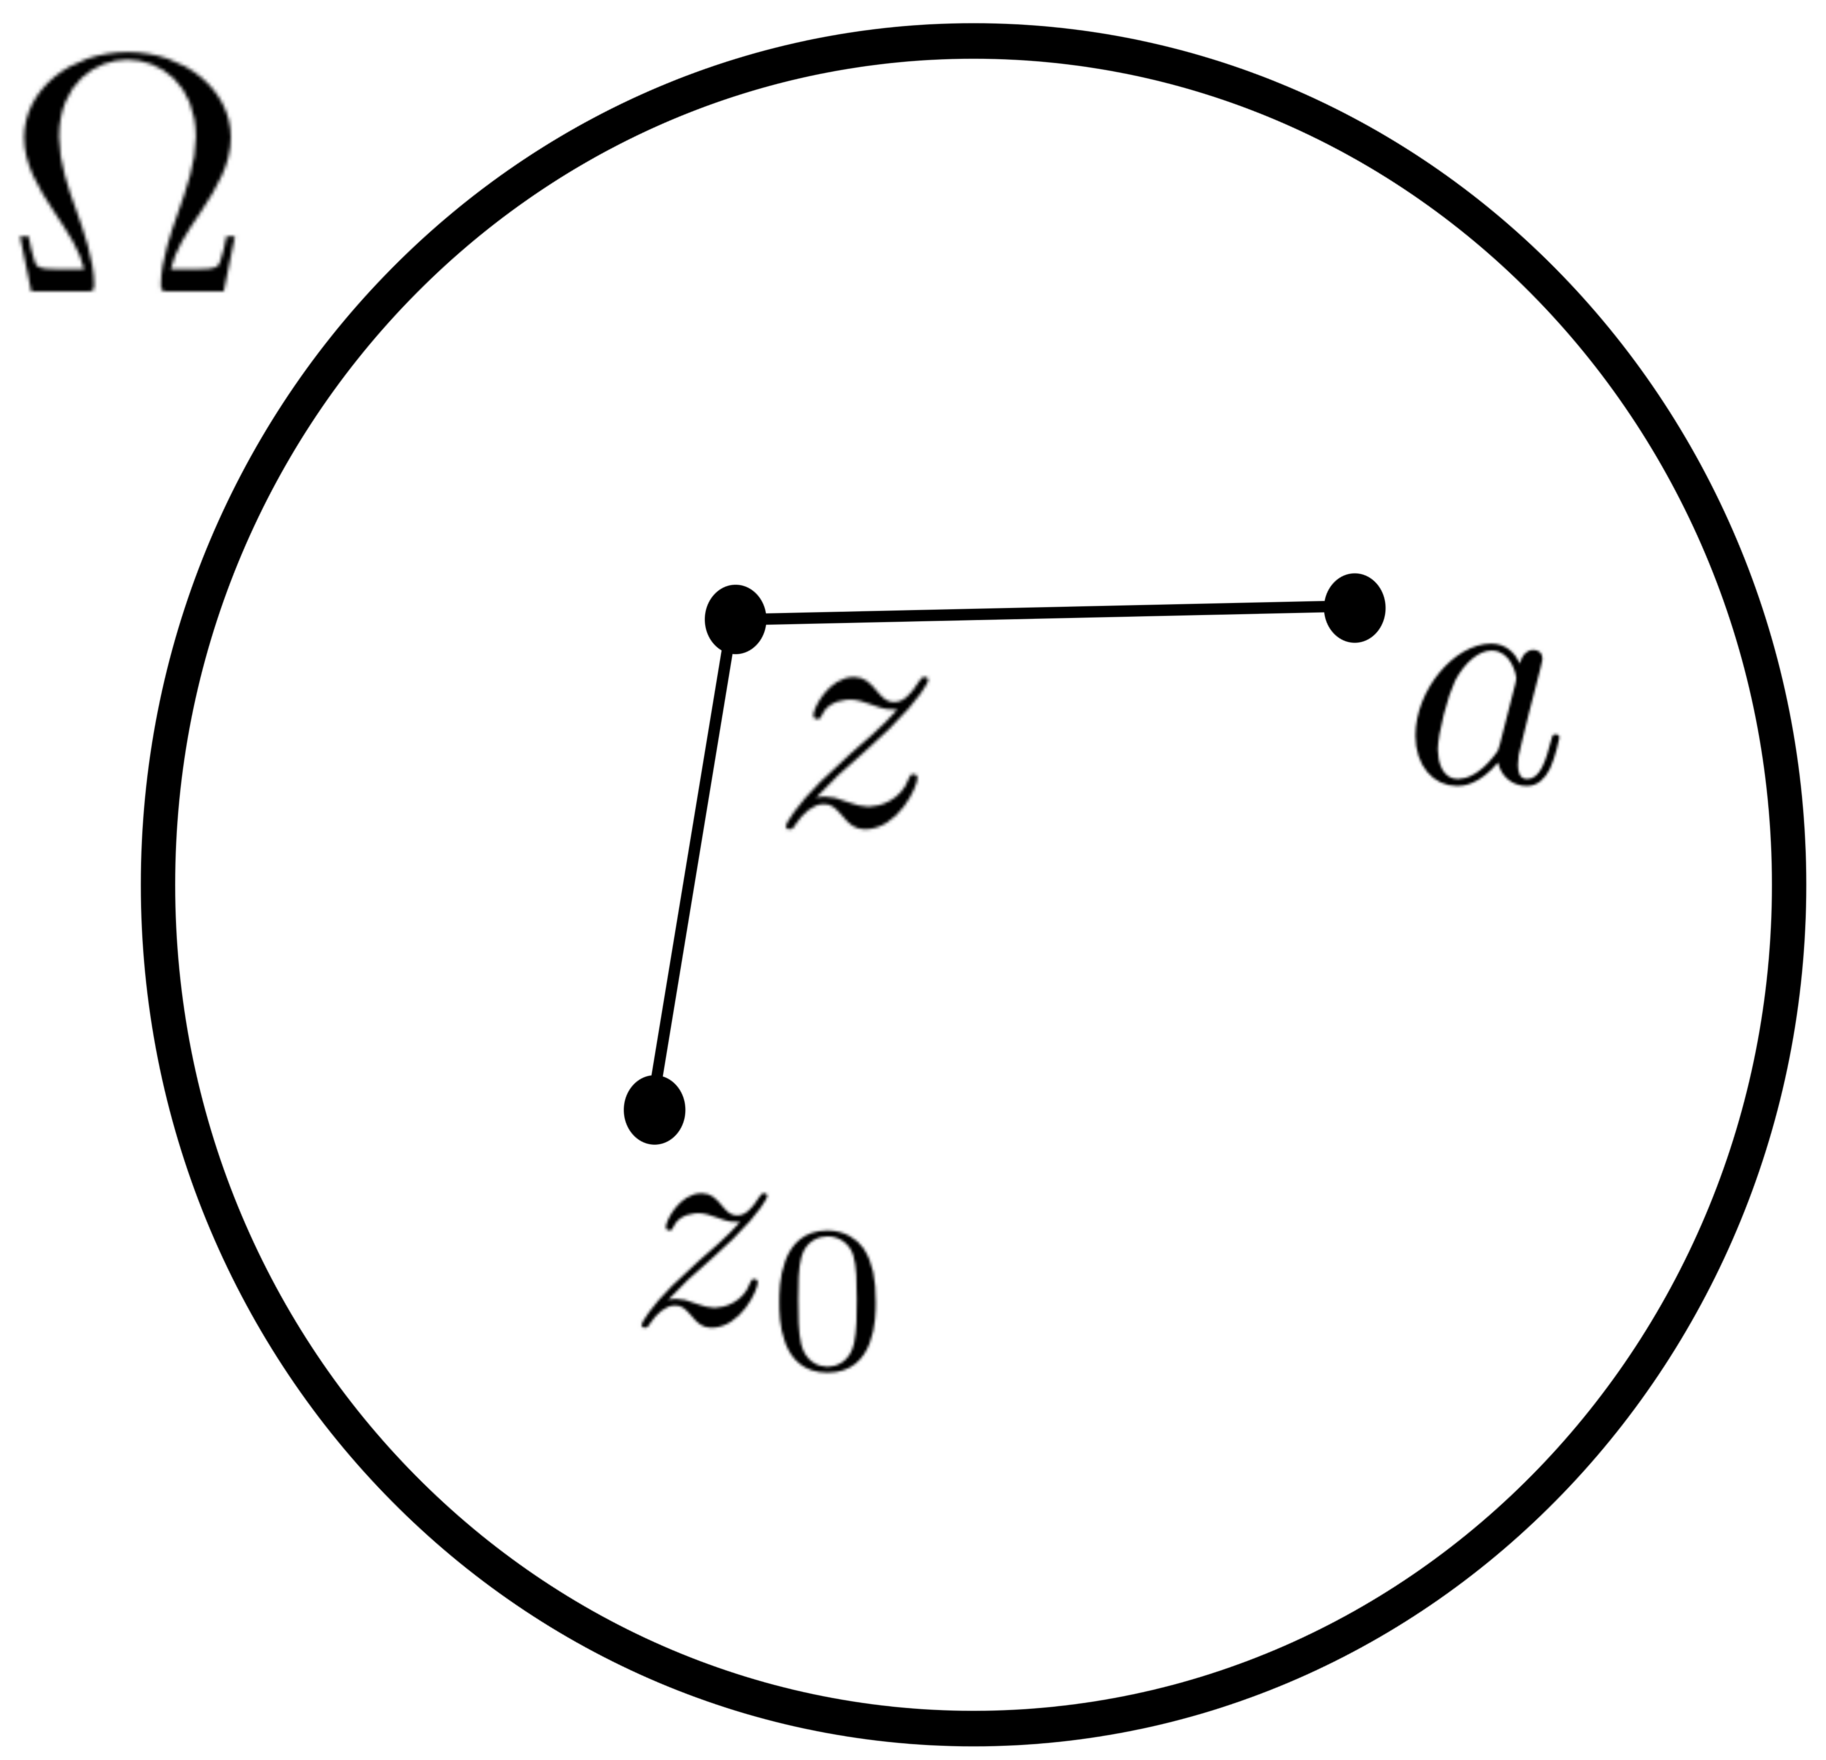
\includegraphics[width=0.2\textwidth]{17.png}
  \end{center}
\end{wrapfigure}

cada $z\in\Omega$ a imagem do intervalo orientado $\left[  a,z\right]  $ está

contida em $\Omega$ e portanto podemos definir a função

$$F:z\in\Omega\longmapsto\underset{\left[  a,z\right]  }{{\displaystyle\int}}f(  \zeta)  d\zeta\in\mathbb{C}.$$

Dados $z\in\Omega$ e $z_{0}\in\Omega,$ a convexidade de $\Omega$ implica

que o tri\^{a}ngulo fechado de vértices $a,z$ \ e $z_{0}$ está

contido em $\Omega$ e como pelo Lema 5.6 temos, se $\Delta=$

$(  a,z,z_{0})  :$\\

\ \ \ \ \ \ \ \ \ \ \ \ \ \ \ \ \ \ \ $\underset{\partial\Delta}{%
%TCIMACRO{\dint }%
%BeginExpansion
{\displaystyle\int}
%EndExpansion
}$ $f=\underset{\left[  a,z\right]  }{%
%TCIMACRO{\dint }%
%BeginExpansion
{\displaystyle\int}
%EndExpansion
}f+\underset{\left[  z,z_{0}\right]  }{%
%TCIMACRO{\dint }%
%BeginExpansion
{\displaystyle\int}
%EndExpansion
}f+\underset{\left[  z_{0},a\right]  }{%
%TCIMACRO{\dint }%
%BeginExpansion
{\displaystyle\int}
%EndExpansion
}f=0$

donde

\bigskip

$(5.7.2)$ \ \ \ \ \ \ \ $\underset{\left[  a,z\right]  }{%
%TCIMACRO{\dint }%
%BeginExpansion
{\displaystyle\int}
%EndExpansion
}f+\underset{\left[  z_{0},a\right]  }{%
%TCIMACRO{\dint }%
%BeginExpansion
{\displaystyle\int}
%EndExpansion
}f=\underset{\left[  z_{0},z\right]  }{%
%TCIMACRO{\dint }%
%BeginExpansion
{\displaystyle\int}
%EndExpansion
}f$.

\bigskip

Por definição de $F$ temos

\bigskip

$(  5.7.3)  $ \ \ \ \ \ $F(  z)  -F(  z_{0})
\underset{\left[  a,z\right]  }{=%
%TCIMACRO{\dint }%
%BeginExpansion
{\displaystyle\int}
%EndExpansion
\text{ }f}-\underset{\left[  a,z_{0}\right]  }{%
%TCIMACRO{\dint }%
%BeginExpansion
{\displaystyle\int}
%EndExpansion
\text{ }f\text{ }}=\underset{\left[  a,z\right]  }{%
%TCIMACRO{\dint }%
%BeginExpansion
{\displaystyle\int}
%EndExpansion
\text{ }f}+\underset{\left[  z_{0},a\right]  }{%
%TCIMACRO{\dint }%
%BeginExpansion
{\displaystyle\int}
%EndExpansion
\text{ }f}$

\bigskip

logo, de $(  5.7.2)  $ e $(  5.7.3)  $ \ resulta

\bigskip

$(  5.7.4)  $ \ \ \ \ \ $F(  z)  -F(  z_{0})
=\underset{\left[  z_{0},z\right]  }{%
%TCIMACRO{\dint }%
%BeginExpansion
{\displaystyle\int}
%EndExpansion
\text{ }f}$ $=\underset{\left[  z_{0},z\right]  }{%
%TCIMACRO{\dint }%
%BeginExpansion
{\displaystyle\int}
%EndExpansion
\text{ }f(  \zeta)  }d\zeta$ $.$

\bigskip

Mostremos que $F^{\prime}(  z_{0})  =f(  z_{0})  .$ De
fato, por $(  5.7.4)  $ temos

\bigskip

$%
%TCIMACRO{\QDABOVE{1pt}{F(  z)  -F(  z_{0})  }{z-z_{0}}}%
%BeginExpansion
\genfrac{}{}{1pt}{0}{F(  z)  -F(  z_{0})  }{z-z_{0}}%
%EndExpansion
-f(  z_{0})  =%
%TCIMACRO{\QDABOVE{1pt}{1}{z-z_{0}}}%
%BeginExpansion
\genfrac{}{}{1pt}{0}{1}{z-z_{0}}%
%EndExpansion
\underset{\left[  z_{0},z\right]  }{%
%TCIMACRO{\dint }%
%BeginExpansion
{\displaystyle\int}
%EndExpansion
\text{ }}\left[  f(  \zeta)  -f(  z_{0})  \right]
d\zeta,$ \ se \ $z\neq z_{0}$ $.$

\bigskip

Dado $\varepsilon>0$ arbitrário, a continuidade de $f$ em $z_{0}$ mostra
que \ existe

$\delta>0$ tal que $\left\vert f(  \zeta)  -f(  z_{0})
\right\vert <\varepsilon$ sempre que $\left\vert \zeta-z_{0}\right\vert
<\delta,$ em conse-

quência, se $z\in\Omega$ e $0<\left\vert z-z_{0}\right\vert <\delta$ temos

\bigskip

$\ \ \ \ \ \ \ \ \ \ \ \left\vert
%TCIMACRO{\QDABOVE{1pt}{F(  z)  -F(  z_{0})  }{z-z_{0}}}%
%BeginExpansion
\genfrac{}{}{1pt}{0}{F(  z)  -F(  z_{0})  }{z-z_{0}}%
%EndExpansion
-f(  z_{0})  \right\vert =\left\vert
%TCIMACRO{\QDABOVE{1pt}{1}{z-z_{0}}}%
%BeginExpansion
\genfrac{}{}{1pt}{0}{1}{z-z_{0}}%
%EndExpansion
\underset{\left[  z_{o},z\right]  }{%
%TCIMACRO{\dint }%
%BeginExpansion
{\displaystyle\int}
%EndExpansion
}\left[  f(  \zeta)  -f(  z_{0})  \right]
d\zeta\right\vert \leq$

\bigskip

$\ \ \ \ \ \ \ \ \ \ \ \ \leq%
%TCIMACRO{\QDABOVE{1pt}{1}{\left\vert z-z_{0}\right\vert }}%
%BeginExpansion
\genfrac{}{}{1pt}{0}{1}{\left\vert z-z_{0}\right\vert }%
%EndExpansion
\underset{\left[  z_{0},z\right]  }{%
%TCIMACRO{\dint }%
%BeginExpansion
{\displaystyle\int}
%EndExpansion
\text{ }}\left\vert f(  \zeta)  -f(  z_{0})  \right\vert
|d\zeta|$ $<%
%TCIMACRO{\QDABOVE{1pt}{\varepsilon}{\left\vert z-z_{0}\right\vert }}%
%BeginExpansion
\genfrac{}{}{1pt}{0}{\varepsilon}{\left\vert z-z_{0}\right\vert }%
%EndExpansion
\underset{\left[  z_{0},z\right]  }{%
%TCIMACRO{\dint }%
%BeginExpansion
{\displaystyle\int}
%EndExpansion
}\left\vert d\zeta\right\vert =\varepsilon$ $,$

\bigskip

o que prova que $F^{\prime}(  z_{0})  =f(  z_{0})  $ e
portanto $F^{\prime}=f$ em $\Omega$ pois $z_{0}$ era

arbitário. Resulta então que $F\in\mathcal{H}(  \Omega)  $
e que $F^{\prime}\in\mathcal{C}(  \Omega)  ,$ donde pela

Prop. 5.4, para cada CSDF $\gamma$ em $\Omega$ temos

\bigskip

\ \ \ \ \ \ \ \ \ \ \ \ \ \ \ \ \ \ \ \ \ \ \ \ \ $\underset{\gamma}{%
%TCIMACRO{\dint }%
%BeginExpansion
{\displaystyle\int}
%EndExpansion
}f(  \zeta)  d\zeta=\underset{\gamma}{%
%TCIMACRO{\dint }%
%BeginExpansion
{\displaystyle\int}
%EndExpansion
}F^{\prime}(  \zeta)  d\zeta=0$ $.\square$

\bigskip

\textbf{Teorema 5.8} \ (fórmula de representação integral de Cauchy)

\textit{Sejam }$\Omega$\textit{\ um aberto convexo não vazio de }$%
%TCIMACRO{\U{2102} }%
%BeginExpansion
\mathbb{C}
%EndExpansion
,$ $\gamma$\textit{\ uma CSDF em }$\Omega$ \textit{e}

$f\in\mathcal{H}(  \Omega)  .$ \textit{Então, para cada }%
$z\in\Omega$ \textit{tal que }$z\notin\gamma^{\ast}$\textit{\ temos:}

\bigskip

\ \ \ \ \ \ \ \ \ \ \ \ \ \ \ \ \ $f(  z)  \cdot$\textsc{I}%
nd$_{\gamma}(  z)  =%
%TCIMACRO{\QDABOVE{1pt}{1}{2\pi i}}%
%BeginExpansion
\genfrac{}{}{1pt}{0}{1}{2\pi i}%
%EndExpansion
\underset{\gamma}{%
%TCIMACRO{\dint }%
%BeginExpansion
{\displaystyle\int}
%EndExpansion
}%
%TCIMACRO{\QDABOVE{1pt}{f(  \zeta)  d\zeta}{\zeta-z}}%
%BeginExpansion
\genfrac{}{}{1pt}{0}{f(  \zeta)  d\zeta}{\zeta-z}%
%EndExpansion
$

\bigskip

Naturalmente, o caso mais interessante é aquele em que \textsc{I}%
nd$_{\gamma}(  z)  =1.$

\bigskip

\textbf{Prova \ }Fixemos $z\in\Omega$ tal que $z\notin\gamma^{\ast},$
então definimos $g:\Omega\rightarrow%
%TCIMACRO{\U{2102} }%
%BeginExpansion
\mathbb{C}
%EndExpansion
$ da

forma seguinte:

\ \ \ \ \ \ \ \ \ \ \ \ \ \ \ \ \ \ \ \ \ \ $g(  \zeta)  :=\left\{
%
\begin{array}
[c]{c}%
%TCIMACRO{\QDABOVE{1pt}{f(  \zeta)  -f(  z)  }{\zeta-z}}%
%BeginExpansion
\genfrac{}{}{1pt}{0}{f(  \zeta)  -f(  z)  }{\zeta-z}%
%EndExpansion
,\text{ \ se \ }\zeta\in\Omega\text{ \ e \ }\zeta\neq z\text{ \ }\\
\\
\text{ \ \ }f^{\prime}(  z)  ,\text{ \ se \ }\zeta=z\text{
\ \ \ \ \ \ \ \ \ \ \ \ \ \ \ \ \ \ \ \ \ \ \ \ \ \ }%
\end{array}
\right.  $

\bigskip

É claro que $g\in\mathcal{C}(  \Omega)  $ e que $g\in
\mathcal{H}(  \Omega\backslash\left\{  z\right\}  )  ,$ portanto
$g$ satisfaz as hipó-

teses do Teor. 5.7, o que implica

\ \ \ \ \ \ \ \ \ \ \ \ \ \ \ \ \ \ \ \ \ \ \ \ \ \ \ \ \ \ \ \ $%
%TCIMACRO{\QDABOVE{1pt}{1}{2\pi i}}%
%BeginExpansion
\genfrac{}{}{1pt}{0}{1}{2\pi i}%
%EndExpansion
\underset{\gamma}{%
%TCIMACRO{\dint }%
%BeginExpansion
{\displaystyle\int}
%EndExpansion
}g(  \zeta)  d\zeta=0$

o que por definição de $g$ (e observando que se $\zeta\in\gamma^{\ast
}$ então $\zeta\neq z$ \ e

portanto só interessa $g|\Omega\backslash\left\{  z\right\}  $) se escreve assim:

\bigskip

\ \ \ \ \ \ \ \ \ \ \ \ \ \ \ \ \ \ \ \ \ \ \ \ \ \ \ \ \ \ \ \ $%
%TCIMACRO{\QDABOVE{1pt}{1}{2\pi i}}%
%BeginExpansion
\genfrac{}{}{1pt}{0}{1}{2\pi i}%
%EndExpansion
\underset{\gamma}{%
%TCIMACRO{\dint }%
%BeginExpansion
{\displaystyle\int}
%EndExpansion
}%
%TCIMACRO{\QDABOVE{1pt}{f(  \zeta)  -f(  z)  }{\zeta-z}}%
%BeginExpansion
\genfrac{}{}{1pt}{0}{f(  \zeta)  -f(  z)  }{\zeta-z}%
%EndExpansion
d\zeta=0$

o que pela definição de \textsc{I}nd$_{\gamma}(  z)  $ pode
ser escrito da maneira seguinte:

\bigskip

\ \ \ \ \ \ \ \ \ \ \ \ \ \ \ \ \ \ \ \ \ \ \ \ \ \ \ \ $%
%TCIMACRO{\QDABOVE{1pt}{1}{2\pi i}}%
%BeginExpansion
\genfrac{}{}{1pt}{0}{1}{2\pi i}%
%EndExpansion
\underset{\gamma}{%
%TCIMACRO{\dint }%
%BeginExpansion
{\displaystyle\int}
%EndExpansion
}%
%TCIMACRO{\QDABOVE{1pt}{f(  \zeta)  d\zeta}{\zeta-z}}%
%BeginExpansion
\genfrac{}{}{1pt}{0}{f(  \zeta)  d\zeta}{\zeta-z}%
%EndExpansion
-f(  z)  \cdot$\textsc{I}nd$_{\gamma}(  z)  =0.$
$\square$

\bigskip

\textbf{Observação \ }O conceito de convexidade é puramente
algébrico, porém

como todo aberto convexo é conexo e a ``conexidade'' é uma propriedade

topológica muito forte, vemos na realidade que a hipótese
(algébrica) de

convexidade tem implicação topológicas muito fortes (conexidade). Entre-

tanto, é importante notar que a conexidade de $\Omega$ não é
suficiente para a

validez do Teor. 5.7, isto é, se no enunciado do Teor. 5.7
substituímos a

hipótese "convexo" por "conexo", o enunciado resultante é falso, como

mostra o exemplo trivial seguinte: $\Omega=%
%TCIMACRO{\U{2102} }%
%BeginExpansion
\mathbb{C}
%EndExpansion
\backslash\left\{  0\right\}  $ é um aberto conexo (mas não

é convexo), a função $f:z\in\Omega\longmapsto1/z\in%
%TCIMACRO{\U{2102} }%
%BeginExpansion
\mathbb{C}
%EndExpansion
$ é holomorfa em $\Omega$ e o círculo

orientado positivamente de centro $0$ e raio $1$ é uma CSDF em $\Omega,$ porém

\bigskip

\ \ \ \ \ \ \ \ \ \ \ \ \ \ \ \ $\underset{\gamma}{%
%TCIMACRO{\dint }%
%BeginExpansion
{\displaystyle\int}
%EndExpansion
}f(  z)  dz=\underset{\gamma}{%
%TCIMACRO{\dint }%
%BeginExpansion
{\displaystyle\int}
%EndExpansion
}%
%TCIMACRO{\QDABOVE{1pt}{dz}{z}}%
%BeginExpansion
\genfrac{}{}{1pt}{0}{dz}{z}%
%EndExpansion
=\underset{0}{%
%TCIMACRO{\dint }%
%BeginExpansion
{\displaystyle\int}
%EndExpansion
}^{2\pi}%
%TCIMACRO{\QDABOVE{1pt}{ie^{it}dt}{e^{it}}}%
%BeginExpansion
\genfrac{}{}{1pt}{0}{ie^{it}dt}{e^{it}}%
%EndExpansion
=2\pi i\neq0.$

\bigskip

A fórmula de representação integral (Teor. 5.8) é uma poderosa
auxiliar no

estudo das propriedades locais das funções holomorfas como ficará bem

claro no próximo resultado que é a recíproca do Teor. 4.6 .

\bigskip

\textbf{Teorema 5.9} \ \ (Goursat) \ \ \textit{Para cada aberto não vazio\ }$\Omega$ \textit{de }$\mathbb{C}$ \textit{temos}

\textit{$\mathcal{H}(\Omega)\subset\mathcal{A}(\Omega)$ e em consequência, pelo Teorema 4.6, temos $\mathcal{H}(\Omega)=\mathcal{A}(\Omega) $}

\bigskip

\textbf{Prova} \ Seja $f\in\mathcal{H}(  \Omega)  .$ Dados
$\zeta\in\Omega$ e $r>0$ tais que $D_{r}(  \zeta)  \subset\Omega,$ vamos

construir uma série de potências em volta de $\zeta$ que representa $f$ em

$D_{r}(  \zeta)  $. suponhamos $r<d=dist(  \zeta,\complement\Omega)$. Então $W:=D_{d}(  \zeta)$ é um aberto

convexo contido em $\Omega$ e se $\gamma_{r}$ é o círculo orientado positivamente de

centro $\zeta$ e raio $r$ \ (isto é $\gamma_{r}:t\in\left[  0,2\pi\right]\longmapsto\zeta+re^{it}\in\mathbb{C}$), como $r<d$

temos $\overline{D}_{r}(  \zeta)  \subset W$ e portanto$ \gamma^{\ast}_{r} \subset W.$ Como $D_{r}(  \zeta)  \cap\gamma^{\ast}_{r} =\varnothing$ e, pela Prop.

5.3 temos \textsc{I}nd$_{\gamma_{r}}(  z)  =1$ para cada $z\in D_{r}(  \zeta)  ,$ podemos aplicar o Teor. 5.8

ao aberto convexo $W=D_{d}(  \zeta)  $ e à CSDF $\gamma_{r}$ obtendo\\


% IMAGEM 18
\begin{wrapfigure}{r}{0.3\textwidth}
  \begin{center}
    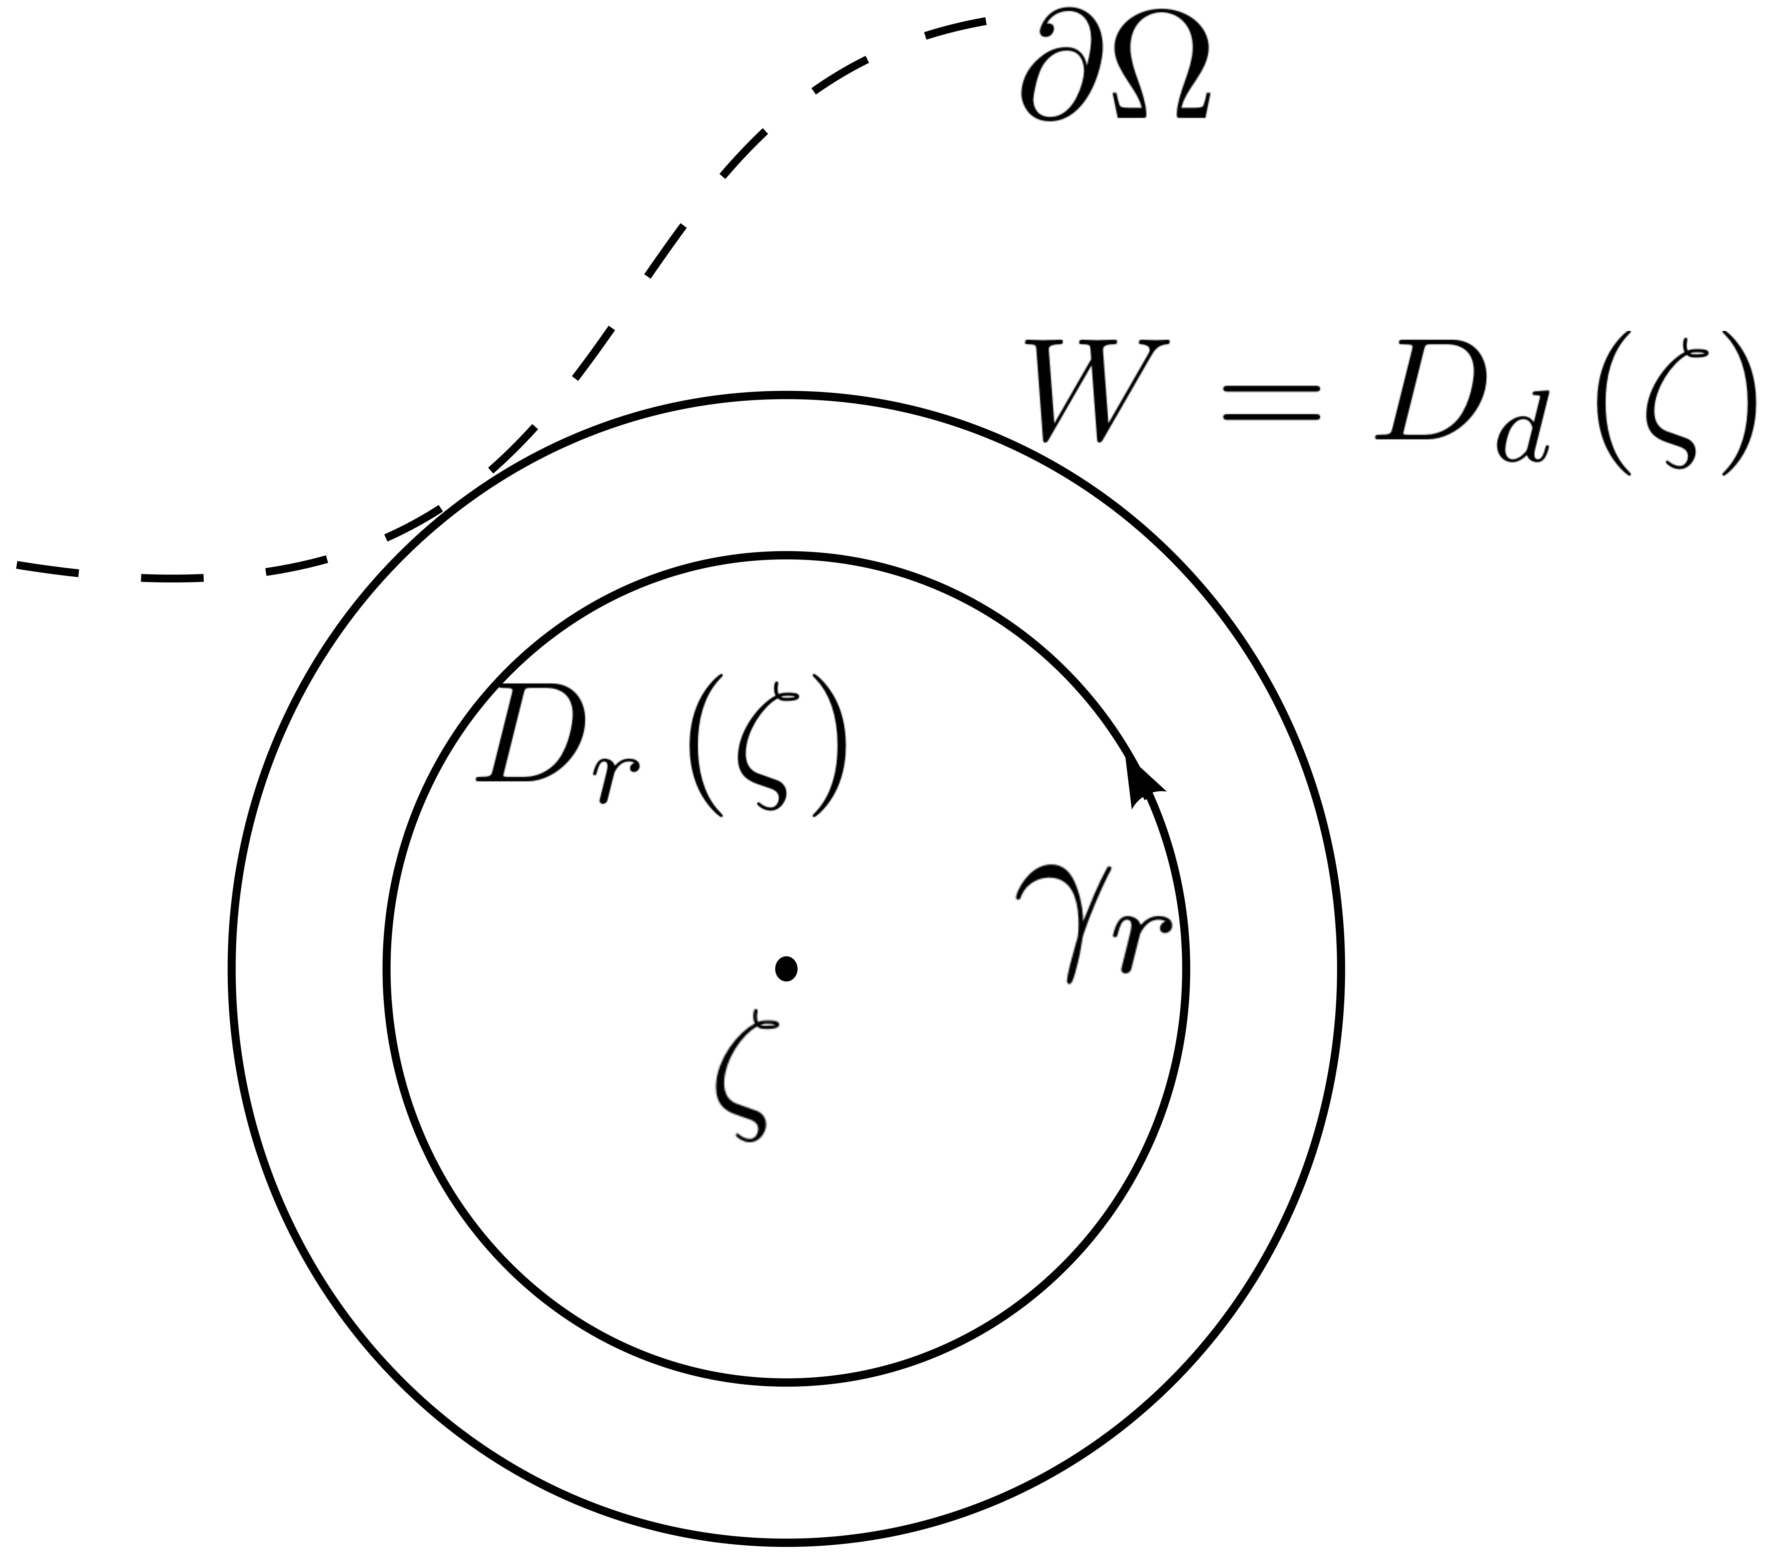
\includegraphics[width=0.3\textwidth]{18.png}
  \end{center}
\end{wrapfigure}

$$f(z) = \genfrac{}{}{1pt}{0}{1}{2\pi i}{\displaystyle\int_{\gamma_{r}}}\genfrac{}{}{1pt}{0}{f(  \lambda)  d\lambda}{\lambda-z} \ \ \ \ \forall  z\in D_{r}(  \zeta).$$

\bigskip

Pela definição de integral curvilinha,

a relação acima pode ser escrita da

forma seguinte:

$$f( z) = \genfrac{}{}{1pt}{0}{1}{2\pi i} \underset{0}{{\displaystyle\int}}^{2\pi}\genfrac{}{}{1pt}{0}{f\left[  \gamma_{r}(  t)  \right]  \gamma_{r}^{\prime}(  t)  dt}{\gamma_{r}(  t)  -z}, \forall z\in D_{r}(\zeta).$$

Pelo Teor. 4.3  resulta então $f\in\mathcal{A}( D_{r}(\zeta))$ e\\\\


$(5.9.1)  $ \ \ $\left\vert
\begin{array}
[c]{c}
\ f(  z)  =\underset{m\geq0}{{\displaystyle\sum}}\left\{\genfrac{}{}{1pt}{0}{1}{2\pi i}\underset{0}{{\displaystyle\int^{2\pi}}}\genfrac{}{}{1pt}{0}{f\left[  \gamma_{r}(  t)  \right]  \gamma_{r}^{\prime}(  t)  dt}{\left[  \gamma_{r}(  t)-\zeta\right]  ^{m+1}}\right\}  (  z-\zeta)  ^{m}=\\
=\underset{m\geq0}{{\displaystyle\sum}}\left\{\genfrac{}{}{1pt}{0}{1}{2\pi i}\underset{\gamma_{r}}{{\displaystyle\int}}\genfrac{}{}{1pt}{0}{f( \gamma) d\gamma}{(\lambda-\zeta)^{m+1}}\right\}(z-\zeta)^{m}
\end{array}\right.  $
\ $\ \ \ \ \ \ \ \ \ \ \ \ \ \ \ \ \ \ \ \ \ \ \ \ \ \ \ \ \ \ \ \ \ \ \ \ \ \ \ \ \ \ \ \ \ \ \ \ $\\

\bigskip

\indent para cada $z\in D_{r}(\zeta),$ sempre que $r\in\left]0,d\right[$. Só resta verificar o caso $r=d$.

Pondo\\

\ \ \ \ \ \ \ \ \ \ \ \ \ \ \ \ \ \ \ \ \ \ \ $c_{m}(  r)  =\genfrac{}{}{1pt}{0}{1}{2\pi i}\underset{\gamma_{r}}{{\displaystyle\int}}\genfrac{}{}{1pt}{0}{f(  \lambda)  d\lambda}{(  \lambda-\zeta)  ^{m+1}}$ \ \ \ \ \ $,$ \ \ \ \ $r\in\left]  0,d\right[  $

\bigskip

é imediato verificar que $c_{m}(  r)  $ independe de r pois
escrevendo $(  5.9.1)  $

para dois valores $r,r^{\prime}\in\left]  0,d\right[  ,$ se por exemplo
$0<r\leq r^{\prime}<d,$ resulta

\bigskip

$\ \ \ \ \ \ \ \ f(z)={\displaystyle\sum}c_{m}(r) (z-\zeta)^{m}={\displaystyle\sum}c_{m}(r^{\prime})  (z-\zeta)^{m} $\ \ \ \ $\forall$ \ \ $z\in D_{r}(\zeta)$\\

donde

\bigskip\ $\ \ \ \ \ \ \ \ \ \ \ \ \ {\displaystyle\sum}\left[  c_{m}(r)-c_{m}( r\prime)  \right] (z-\zeta)^{m}=0$ \ \ $\forall$ \ \ $z\in D_{r}(\zeta)  $\ \ \ \ \ $(r\leq r^{\prime})$\\

o que pelo exerc. 3.5 implica $c_{m}(  r)  =c_{m}(  r^{\prime})  $ \ sempre que $r,r^{\prime}\in\left]  0,d\right[  .$

Vamos indicar por $c_{m}$ este valor independente de $r$, isto é:

\bigskip

\ \ \ \ \ \ \ \ \ \ \ \ \ \ \ \ \ \ \ \ \ \ \ \ \ $c_{m}=\genfrac{}{}{1pt}{0}{1}{2\pi i}\underset{\gamma_{r}}{{\displaystyle\int}}\genfrac{}{}{1pt}{0}{f(\lambda) d\lambda}{( \lambda-\zeta)^{m+1}}$ \ \ \ \ $\forall$ \ \ \ $r\in\left] 0,d\right[$\\

então $(  5.9.1)  $ se escreve:\\

\ \ \ \ \ \ \ \ \ \ \ \ \ \ \ \ \ \ \ \ \ \ \ \ \ \ \ \ \ \ \ \ $f(z)={\displaystyle\sum}c_{m}(  z-\zeta)  ^{m}$ \ \ \ \ $\forall$ \ \ \ $z\in D_{r}(\zeta)$\\

sempre que $r<d.$ Resulta então (ver Obs. $\left[  2\right]  ,$ logo após a Def. 4.1 que

o raio de convergência $\rho$ \ da série acima é $\geq r,$ para cada $r<d,$ donde

$\rho\geq d,$ portanto

\ \ \ \ \ \ \ \ \ \ \ \ \ \ \ \ \ \ \ \ \ \ \ \ \ \ \ $f(  z)  ={\displaystyle\sum}c_{m}(  z-\zeta)  ^{m}$ \ \ \ $\forall$ \ \ $z\in D_{d}(\zeta) ,$\\

o que prova que $f\in\mathcal{A}(  \Omega)  .$ $\square$

\bigskip

\textbf{Corolário 5.10 \ }\textit{Sejam }$\Omega$\textit{\ um aberto não vazio, }$f\in\mathcal{H}( \Omega)  $ \textit{e }
$\overline{D}_{r}(  \zeta)  \subset\Omega.$

\textit{Se }$\gamma:t\in\left[  0,2\pi\right]  \longmapsto\zeta+re^{it}\in \mathbb{C}$ 
\textit{é o círculo orientado positivamente} de 

centro $\zeta$ \textit{\ e raio }$r,$ \textit{então}

\bigskip

$(5.10.1) $ \ \ \ $f^{(m)}(\zeta) =\genfrac{}{}{1pt}{0}{m!}{2\pi i}\underset{\gamma}{{\displaystyle\int}}\genfrac{}{}{1pt}{0}{f(\lambda) d\lambda}{(\lambda-\zeta)^{m+1}}=\genfrac{}{}{1pt}{0}{m!}{2\pi i}
\underset{\left\vert \lambda-\zeta\right\vert =r}{{\displaystyle\int}}\genfrac{}{}{1pt}{0}{f(\lambda) d\lambda}{( \lambda-\zeta)^{m+1}}$ \ \ $\forall$ \ $m\in
\mathbb{N}$

\bigskip

\textbf{Prova \ \ }Usar $(  5.9.1)  $ e o Corol. 4.9. \ $\square$

\bigskip

\textbf{Corolário 5.11 \ }(Desigualdades de Cauchy) \ \textit{Sejam} $\Omega$ \textit{um aberto não}

\textit{vazio de }$\mathbb{C},$ $f\in\mathcal{H}(  \Omega)  $ \textit{e }$\overline{D}_{r}(  \zeta)  \subset\Omega.$ \textit{Então, }

\ \ \ \ \ \ \ \ \ \ \ \ \ \ \ \ \ \ \ \ \ \ \ \ \ \ \ \ \ \ 

\ \ \ \ \ \ \ \ \ \ \ \ \ \ \ \ \ \ \ \ \ \ \ \ $\left\vert f^{(m)  }(  \zeta)  \right\vert \leq
\genfrac{}{}{1pt}{0}{m!}{r^{m}}\underset{\left\vert z-\zeta\right\vert =r}{\sup}\left\vert f(z)\right\vert ,$ \ \textit{para cada }$m\in\mathbb{N}.$

\bigskip

\textbf{Prova} \ As hipóteses sendo as mesmas do Corol. 5.10, podemos usar

$(  5.10.1)  ,$ que junto com a desigualdade $(  5.1.6)
$ \ prova o resultado. \ $\square$

\bigskip

\textbf{\ Corolário 5.12 } (teorema de Liouiville) \ \textit{Se }%
$f\in\mathcal{H}(
%TCIMACRO{\U{2102} }%
%BeginExpansion
\mathbb{C}
%EndExpansion
)  $ \textit{e é limitada }(isto

é, existe $M>0$ tal que $\left\Vert f\right\Vert _{%
%TCIMACRO{\U{2102} }%
%BeginExpansion
\mathbb{C}
%EndExpansion
}\leq M$), \textit{então }$f$ é constante.

\bigskip

\textbf{Prova \ }Pelo Corol. 4.11 podemos escrever

\bigskip

$(  5.12.1)  $ \ \ \ \ \ $f(  z)  =\underset{m\geq0}{%
%TCIMACRO{\dsum }%
%BeginExpansion
{\displaystyle\sum}
%EndExpansion
}%
%TCIMACRO{\QDABOVE{1pt}{1}{m!}}%
%BeginExpansion
\genfrac{}{}{1pt}{0}{1}{m!}%
%EndExpansion
f^{(  m)  }(  0)  z^{m},$ \ para cada $z\in%
%TCIMACRO{\U{2102} }%
%BeginExpansion
\mathbb{C}
%EndExpansion
.$

\bigskip

Mostremos que $f^{(  m)  }(  0)  =0$ para cada $m\geq1.$
De fato, pelo Corol. 5.11

temos:

\bigskip

$(  5.12.2)  $ \ \ \ \ \ \ \ \ \ \ \ \ \ $\left\vert f^{(
m)  }(  0)  \right\vert \leq%
%TCIMACRO{\QDABOVE{1pt}{m!}{r^{m}}}%
%BeginExpansion
\genfrac{}{}{1pt}{0}{m!}{r^{m}}%
%EndExpansion
\underset{\left\vert z\right\vert =r}{\sup}\left\vert f(  z)
\right\vert ,$ \ \ $\forall$ \ $m\geq1$ \ $,$ \ $\forall$ \ $r>0$

\bigskip

Por outro lado a hipótese de limitação sobre $f$ acarreta

\ \ \ \ \ \ \ \ \ \ \ \ \ \ \ \ \ \ \ \ \ \ \ \ \ \ \ \ $\underset{\left\vert
z\right\vert =r}{\sup}\left\vert f(  z)  \right\vert \leq\left\Vert
f\right\Vert _{%
%TCIMACRO{\U{2102} }%
%BeginExpansion
\mathbb{C}
%EndExpansion
}\leq M$ \ \ \ \ \ $,$ \ \ $\forall$ \ \ \ $r>0$

logo de $(  5.12.2)  $ \ resulta

\bigskip\ \ \ \ \ \ \ \ \ \ \ \ \ \ \ \ \ \ \ \ \ \ \ \ \ \ \ \ \ $\left\vert
f^{(  m)  }(  0)  \right\vert \leq%
%TCIMACRO{\QDABOVE{1pt}{m!}{r^{m}}}%
%BeginExpansion
\genfrac{}{}{1pt}{0}{m!}{r^{m}}%
%EndExpansion
M$ \ $,$ \ \ $\forall$ \ $m\geq1$ \ $,$ \ $\forall$ \ $r>0$

\bigskip

e em consequência, para cada $m\geq1$ \ \textit{fixado \ }resulta

\bigskip

\ \ \ \ \ \ \ \ \ \ \ \ \ \ \ \ $\left\vert f^{(  m)  }(
0)  \right\vert \leq\underset{r\rightarrow+\infty}{\lim}(
%TCIMACRO{\QDABOVE{1pt}{m!M}{r^{m}}}%
%BeginExpansion
\genfrac{}{}{1pt}{0}{m!M}{r^{m}}%
%EndExpansion
)  =Mm!\underset{r\rightarrow+\infty}{\lim}%
%TCIMACRO{\QDABOVE{1pt}{1}{r^{m}}}%
%BeginExpansion
\genfrac{}{}{1pt}{0}{1}{r^{m}}%
%EndExpansion
=0$ \ $,$ \ pois \ $m\geq1.$

\bigskip

Desta forma, de $(  5.12.1)  $ resulta $f(  z)
=f(  0)  $ \ para cada $z\in%
%TCIMACRO{\U{2102} }%
%BeginExpansion
\mathbb{C}
%EndExpansion
.$ \ $\square$

\bigskip

\textbf{Corolário 5.13} \ (teorema fundamental da álgebra)
\ \textit{Todo polinômio}

\textit{com coeficientes complexos de grau }$m\geq1,$ \textit{possui pelo
menos uma}

\textit{raiz.}

\bigskip

\textbf{Prova \ }\ Seja $f(  z)  =\underset{k=0}{\overset{m}{%
%TCIMACRO{\dsum }%
%BeginExpansion
{\displaystyle\sum}
%EndExpansion
}}a_{k\text{ }}z^{k}$ \ o polinômio, então $a_{m}\neq0.$ Suponhamos

por absurdo que $f$ não possui nenhuma rais, isto é, $f(
z)  \neq0$ \ $\forall$ \ $z\in%
%TCIMACRO{\U{2102} }%
%BeginExpansion
\mathbb{C}
%EndExpansion
.$

Resulta então que a função

\ \ \ \ \ \ \ \ \ \ \ \ \ \ \ \ \ \ \ \ \ \ \ \ \ \ \ \ \ \ \ \ $g:z\in%
%TCIMACRO{\U{2102} }%
%BeginExpansion
\mathbb{C}
%EndExpansion
\longmapsto%
%TCIMACRO{\QDABOVE{1pt}{1}{f(  z)  }}%
%BeginExpansion
\genfrac{}{}{1pt}{0}{1}{f(  z)  }%
%EndExpansion
\in%
%TCIMACRO{\U{2102} }%
%BeginExpansion
\mathbb{C}
%EndExpansion
$

é holomorfa em $%
%TCIMACRO{\U{2102} }%
%BeginExpansion
\mathbb{C}
%EndExpansion
$ (Exemplo 3, Cap 1). Como $a_{m}\neq0,$ é evidente que existe

$\rho>0$ tal que

\bigskip\ $\ \ \ \ \ \ \ \ \ \ \ \ \ \ \ \ \ \ \ \ \ \ \ \
%TCIMACRO{\QDABOVE{1pt}{\left\vert a_{m-1}\right\vert }{\left\vert z\right\vert
%}}%
%BeginExpansion
\genfrac{}{}{1pt}{0}{\left\vert a_{m-1}\right\vert }{\left\vert z\right\vert }%
%EndExpansion
+\cdots\cdots+%
%TCIMACRO{\QDABOVE{1pt}{\left\vert a_{0}\right\vert }{\left\vert z\right\vert
%^{m}}}%
%BeginExpansion
\genfrac{}{}{1pt}{0}{\left\vert a_{0}\right\vert }{\left\vert z\right\vert
^{m}}%
%EndExpansion
<%
%TCIMACRO{\QDABOVE{1pt}{\left\vert a_{m}\right\vert }{2}}%
%BeginExpansion
\genfrac{}{}{1pt}{0}{\left\vert a_{m}\right\vert }{2}%
%EndExpansion
$ \ $,$ \ \ se $\left\vert z\right\vert >\rho$

portanto:

\ \ \ \ \ \ \ \ \ \ \ $\left\vert f(  z)  \right\vert =\left\vert
a_{m}z^{m}+\cdots+a_{0}\right\vert =\left\vert z\right\vert ^{m}%
\cdot\left\vert a_{m}+%
%TCIMACRO{\QDABOVE{1pt}{a_{m-1}}{z}}%
%BeginExpansion
\genfrac{}{}{1pt}{0}{a_{m-1}}{z}%
%EndExpansion
+\cdots+%
%TCIMACRO{\QDABOVED{.}{.}{1pt}{a_{0}}{z^{m}}}%
%BeginExpansion
\genfrac{.}{.}{1pt}{0}{a_{0}}{z^{m}}%
%EndExpansion
\right\vert \geq$

$\geq\left\vert z\right\vert ^{m}\left\vert \left\vert a_{m}\right\vert
-\left\vert
%TCIMACRO{\QDABOVE{1pt}{a_{m-1}}{z}}%
%BeginExpansion
\genfrac{}{}{1pt}{0}{a_{m-1}}{z}%
%EndExpansion
+\cdots+%
%TCIMACRO{\QDABOVE{1pt}{a_{0}}{z^{m}}}%
%BeginExpansion
\genfrac{}{}{1pt}{0}{a_{0}}{z^{m}}%
%EndExpansion
\right\vert \right\vert \geq\left\vert z\right\vert ^{m}\cdot\left\vert
\left\vert a_{m}\right\vert -(
%TCIMACRO{\QDABOVE{1pt}{\left\vert a_{m-1}\right\vert }{\left\vert z\right\vert
%}}%
%BeginExpansion
\genfrac{}{}{1pt}{0}{\left\vert a_{m-1}\right\vert }{\left\vert z\right\vert }%
%EndExpansion
+\cdots+%
%TCIMACRO{\QDABOVE{1pt}{\left\vert a_{0}\right\vert }{\left\vert z\right\vert
%^{m}}}%
%BeginExpansion
\genfrac{}{}{1pt}{0}{\left\vert a_{0}\right\vert }{\left\vert z\right\vert
^{m}}%
%EndExpansion
)  \right\vert >$

$>\left\vert z\right\vert ^{m}\cdot(  \left\vert a_{m}\right\vert -%
%TCIMACRO{\QDABOVE{1pt}{\left\vert a_{m}\right\vert }{2}}%
%BeginExpansion
\genfrac{}{}{1pt}{0}{\left\vert a_{m}\right\vert }{2}%
%EndExpansion
)  =%
%TCIMACRO{\QDABOVE{1pt}{\left\vert a_{m}\right\vert \left\vert z\right\vert
%^{m}}{2}}%
%BeginExpansion
\genfrac{}{}{1pt}{0}{\left\vert a_{m}\right\vert \left\vert z\right\vert
^{m}}{2}%
%EndExpansion
$ \ $,$ \ sempre que $\left\vert z\right\vert >\rho.$

\bigskip

Seja $r=\max(  \rho,\sqrt[m]{%
%TCIMACRO{\QDABOVE{1pt}{2}{\left\vert a_{m}\right\vert }}%
%BeginExpansion
\genfrac{}{}{1pt}{0}{2}{\left\vert a_{m}\right\vert }%
%EndExpansion
})  $ \ , então o cálculo anterior mostra que

\ \ \ \ \ \ \ \ \ \ \ $\left\vert f(  z)  \right\vert >1$ \ ,
\ para cada $z\in%
%TCIMACRO{\U{2102} }%
%BeginExpansion
\mathbb{C}
%EndExpansion
\backslash\overline{D}_{r}(  0)  $

e em consequência

\bigskip

$(  5.13.1)  $ \ \ \ \ \ \ \ \ \ \ \ \ \ \ \ $\left\vert g(
z)  \right\vert <1$ \ , \ para cada $z\in%
%TCIMACRO{\U{2102} }%
%BeginExpansion
\mathbb{C}
%EndExpansion
\backslash\overline{D}_{r}(  0)  $

\bigskip\ 

Por outro lado, como $\overline{D}_{r}(  0)  $ \ é compacto e
$\left\vert g\right\vert $ \ é contínua em $\overline{D}_{r}(
0)  ,$ é

claro que $\left\vert g\right\vert $ \ é limitada em $\overline{D}%
_{r}(  0)  ,$ isto é, existe $L>0$ tal que

\bigskip

$(  5.13.2)  $ \ \ \ \ \ \ \ $\left\vert g(  z)
\right\vert \leq L$ \ para cada $z\in\overline{D}_{r}(  0)  $

\bigskip

De $(  5.13.1)  $ e $(  5.13.2)  $ resulta

\ \ \ \ \ \ \ \ \ \ \ \ \ \ \ \ \ \ \ \ $\left\vert g(  z)
\right\vert \leq M=\max(  1,L)  $ $,$ para cada $z\in%
%TCIMACRO{\U{2102} }%
%BeginExpansion
\mathbb{C}
%EndExpansion
$

isto é, $g$ é limitada, logo, pelo Corol. 5.12 resulta que $g$ é
constante o

que acarreta que $f$ é constante o que é absurdo pois sendo $\partial
f=m\geq1,$

$f$ não pode ser constante pelo princípio de identidade de
polinômios. \ $\square$

\bigskip

A próxima propriedade importante das funções analíticas que
vamos ver

é o princípio do módulo máximo e a parte essencial da prova
está contida

no seguinte:

\bigskip

\textbf{Lema 5.14 \ }\textit{Sejam }$\zeta\in%
%TCIMACRO{\U{2102} }%
%BeginExpansion
\mathbb{C}
%EndExpansion
,$ $\rho>0$ \textit{e }$f\in\mathcal{H}(  D_{\rho}(  \zeta)
)  .$ \textit{Se}

\bigskip

$(  5.14.1)  $ \ \ \ \ \ \ \ \ \ \ \ \ \ \ \ \ \ \ \ \ $\left\vert
f(  z)  \right\vert \leq\left\vert f(  \zeta)
\right\vert $ \ \textit{para cada }$z\in D_{\rho}(  \zeta)  ,$

\bigskip

\textit{então }$f(  z)  =f(  \zeta)  $ \textit{para
cada }$z\in D_{\rho}(  \zeta)  .$

\bigskip

\textbf{Prova \ }O resultado é trivial se $f(  \zeta)  =0$
portanto podemos supor que

$f(  \zeta)  \neq0.$ Pela fórmula de representação
integral (Teor. 5.8) e pela Prop.

5.3, para cada $r\in\left]  0,\rho\right[  $ temos:

\ \ \ \ \ \ \ \ \ \ \ \ \ \ \ \ $f(  \zeta)  =%
%TCIMACRO{\QDABOVE{1pt}{1}{2\pi i}}%
%BeginExpansion
\genfrac{}{}{1pt}{0}{1}{2\pi i}%
%EndExpansion%
%TCIMACRO{\dint _{\left\vert \lambda-\zeta\right\vert =r}}%
%BeginExpansion
{\displaystyle\int_{\left\vert \lambda-\zeta\right\vert =r}}
%EndExpansion%
%TCIMACRO{\QDABOVE{1pt}{f(  \lambda)  d\lambda}{\lambda-\zeta}}%
%BeginExpansion
\genfrac{}{}{1pt}{0}{f(  \lambda)  d\lambda}{\lambda-\zeta}%
%EndExpansion
=%
%TCIMACRO{\QDABOVE{1pt}{1}{2\pi}}%
%BeginExpansion
\genfrac{}{}{1pt}{0}{1}{2\pi}%
%EndExpansion
\underset{0}{%
%TCIMACRO{\dint }%
%BeginExpansion
{\displaystyle\int}
%EndExpansion
}^{2\pi}f(  \zeta+re^{it})  dt$

e como $f(  \zeta)  =%
%TCIMACRO{\QDABOVE{1pt}{1}{2\pi}}%
%BeginExpansion
\genfrac{}{}{1pt}{0}{1}{2\pi}%
%EndExpansion
\underset{0}{%
%TCIMACRO{\dint }%
%BeginExpansion
{\displaystyle\int}
%EndExpansion
}^{2\pi}f(  \zeta)  dt,$ podemos escrever

\ \ \ \ \ \ \ \ \ \ \ $0=f(  \zeta)  -f(  \zeta)  =%
%TCIMACRO{\QDABOVE{1pt}{1}{2\pi}}%
%BeginExpansion
\genfrac{}{}{1pt}{0}{1}{2\pi}%
%EndExpansion
\underset{0}{%
%TCIMACRO{\dint }%
%BeginExpansion
{\displaystyle\int}
%EndExpansion
}^{2\pi}\left[  f(  \zeta)  -f(  \zeta+re^{it})
\right]  dt,$ \ $\forall$ \ $r\in\left]  0,\rho\right[  $

e sendo $f(  \zeta)  \neq0,$ resulta

\bigskip

$(  5.14.2)  $ \ \ \ \ $\underset{0}{%
%TCIMACRO{\dint }%
%BeginExpansion
{\displaystyle\int}
%EndExpansion
}^{2\pi}\left[  1-%
%TCIMACRO{\QDABOVE{1pt}{f(  \zeta+re^{it})  }{f(  \zeta)
%}}%
%BeginExpansion
\genfrac{}{}{1pt}{0}{f(  \zeta+re^{it})  }{f(  \zeta)  }%
%EndExpansion
\right]  dt=0$ \ $,$ \ $\forall$ \ $r\in\left]  0,\rho\right[  $

e em particular, a parte real desta integral é nula, isto é,

\bigskip

$(  5.14.3)  $ \ \ \ $\underset{0}{%
%TCIMACRO{\dint }%
%BeginExpansion
{\displaystyle\int}
%EndExpansion
}^{2\pi}\left[  1-\operatorname{Re}(
%TCIMACRO{\QDABOVE{1pt}{f(  \zeta+re^{it})  }{f(  \zeta)
%}}%
%BeginExpansion
\genfrac{}{}{1pt}{0}{f(  \zeta+re^{it})  }{f(  \zeta)  }%
%EndExpansion
)  \right]  dt=0$ \ $,$ \ $\forall$ \ $r\in\left[  0,\rho\right]  $ \ .

Para cada $r\in\left]  0,\rho\right[  $ e para cada $t\in\left[
0,2\pi\right]  ,$ a hipótese $(  5.14.1)  $ implica

\bigskip

$\ \ \ \ \ \ \operatorname{Re}(
%TCIMACRO{\QDABOVE{1pt}{f(  \zeta+re^{it})  }{f(  \zeta)
%}}%
%BeginExpansion
\genfrac{}{}{1pt}{0}{f(  \zeta+re^{it})  }{f(  \zeta)  }%
%EndExpansion
)  \leq\left\vert \operatorname{Re}(
%TCIMACRO{\QDABOVE{1pt}{f(  \zeta+re^{it})  }{f(  \zeta)
%}}%
%BeginExpansion
\genfrac{}{}{1pt}{0}{f(  \zeta+re^{it})  }{f(  \zeta)  }%
%EndExpansion
)  \right\vert \leq\left\vert
%TCIMACRO{\QDABOVE{1pt}{f(  \zeta+re^{it})  }{f(  \zeta)
%}}%
%BeginExpansion
\genfrac{}{}{1pt}{0}{f(  \zeta+re^{it})  }{f(  \zeta)  }%
%EndExpansion
\right\vert \leq1$

donde

\ \ \ \ \ \ \ \ $1-\operatorname{Re}(
%TCIMACRO{\QDABOVE{1pt}{f(  \zeta+re^{it})  }{f(  \zeta)
%}}%
%BeginExpansion
\genfrac{}{}{1pt}{0}{f(  \zeta+re^{it})  }{f(  \zeta)  }%
%EndExpansion
)  \geq0$ \ \ \ \ \ $\forall$ \ \ $r\in\left]  0,\rho\right[  $ $,$
\ $\forall$ \ $t\in\left[  0,2\pi\right]  $

o que junto a $(  5.14.3)  $ implica

\ \ \ \ \ \ \ \ \ \ $\operatorname{Re}(
%TCIMACRO{\QDABOVE{1pt}{f(  \zeta+re^{it})  }{f(  \zeta)
%}}%
%BeginExpansion
\genfrac{}{}{1pt}{0}{f(  \zeta+re^{it})  }{f(  \zeta)  }%
%EndExpansion
)  =1$ \ \ \ $\forall$ \ \ $r\in\left]  0,\rho\right[  $ $,$ \ $\forall$
\ $t\in\left[  0,2\pi\right]  $

ou seja

$\bigskip(  5.14.4)  $
\ \ \ \ \ \ \ \ \ \ \ \ \ \ \ $\operatorname{Re}(
%TCIMACRO{\QDABOVE{1pt}{f(  z)  }{f(  \zeta)  }}%
%BeginExpansion
\genfrac{}{}{1pt}{0}{f(  z)  }{f(  \zeta)  }%
%EndExpansion
)  =1$ \ \ \ \ \ \ $\forall$ \ $z\in D_{\rho}(  \zeta)  .$

Seja $g:D_{\rho}(  \zeta)  \rightarrow%
%TCIMACRO{\U{2102} }%
%BeginExpansion
\mathbb{C}
%EndExpansion
$ \ a função definida por

\ \ \ \ \ \ \ \ \ \ \ \ \ \ \ \ \ \ \ \ 

\ \ \ \ \ \ \ \ \ \ \ \ \ \ \ \ \ \ \ \ \ \ \ \ $g(  z)  :=%
%TCIMACRO{\QDABOVE{1pt}{f(  z)  }{f(  \zeta)  }}%
%BeginExpansion
\genfrac{}{}{1pt}{0}{f(  z)  }{f(  \zeta)  }%
%EndExpansion
$ \ \ para cada \ $z\in D_{\rho}(  \zeta)  $

então é claro que $g\in\mathcal{H}(  D_{\rho}(
\zeta)  )  $ e como $D_{\rho}(  \zeta)  $ é um
aberto conexo, a

relação $(  5.14.4)  $ \ e a Prop. 2.6 implicam que $g$
é constante em $D_{\rho}(  \zeta)  .$

Mas a definição de $g$ mostra que $g(  \zeta)  =1,$ em consequência

\ \ \ \ \ \ \ \ \ \ \ \ \ \ \ \ \ \ \ \ \ \ $g(  z)  =%
%TCIMACRO{\QDABOVE{1pt}{f(  z)  }{f(  \zeta)  }}%
%BeginExpansion
\genfrac{}{}{1pt}{0}{f(  z)  }{f(  \zeta)  }%
%EndExpansion
=1$ \ \ \ \ \ \ \ \ para cada \ $z\in D_{\rho}(  \zeta)  $

o que demonstra o resultado. \ $\square$

\bigskip

\textbf{Teorema 5.15 \ }(Princípio do módulo máximo)
\ \ \textit{Sejam }$\Omega$ \textit{um aberto}

\textit{limitado e }$f\in\mathcal{H}(  \Omega)  \cap\mathcal{C}%
(  \overline{\Omega})  .$ \textit{Então, o máximo de
}$\left\vert f\right\vert $ \textit{em }$\overline{\Omega}$ \textit{é
atingido }

\textit{em }$\partial\Omega.$

\bigskip

\textbf{Prova \ }Como $\Omega$ é limitado, $\overline{\Omega}$ é
compacto e, sendo $\left\vert f\right\vert $ contínua em $\overline
{\Omega},$

esta função tem um máximo, isto é, existe $\zeta\in
\overline{\Omega}$ tal que

\bigskip

$(  5.15.1)  $ \ \ \ \ \ \ \ \ \ \ \ \ \ \ \ $\underset
{z\in\overline{\Omega}}{\max}\left\vert f(  z)  \right\vert
=\left\vert f(  \zeta)  \right\vert .$

\bigskip

Se $\zeta\in\partial\Omega$ não há o que demonstrar de modo que
podemos supor que

$\zeta\in\Omega$ e neste caso vamos provar que existe $\xi\in\partial\Omega$
tal que $\left\vert f(  \xi)  \right\vert =$

$\left\vert f(  \zeta)  \right\vert .$ Como $\zeta\in\Omega,$
existe $\rho>0$ tal que $D_{\rho}(  \zeta)  \subset\Omega$ e
então por $(  5.15.1)  $

e pelo Lema 5.14 resulta

\ \ \ \ \ \ \ \ \ \ \ \ \ \ \ \ \ \ \ \ \ \ \ \ \ \ \ \ $f(  z)
=f(  \zeta)  ,$ \ \ \ \ \ \ $\forall$ \ \ $z\in D_{\rho}(
\zeta)  $

o que mostra que $f$ é constante sobre $D_{\rho}(  \zeta)  ,$
logo pelo Teor. 4.12, $f$ é

constante sobre a componente conexa $\Omega_{0}$ de $\Omega$ que contem
$\zeta.$ Como

$f\in\mathcal{C}(  \overline{\Omega})  $ e portanto $f|\overline
{\Omega}_{0}\in\mathcal{C}(  \overline{\Omega}_{0})  $ resulta que
$f$ é constante sobre $\overline{\Omega}_{0}.$

Como $\varnothing\neq\partial\Omega_{0}\subset\overline{\Omega}_{0},$ existe
$\xi\in\partial\Omega_{0}$ e então $f(  \zeta)  =f(
\xi)  ,$ portanto de

$(  5.15.1)  $ segue

\ \ \ \ \ \ \ \ \ \ \ \ \ \ \ \ \ \ \ \ \ \ \ \ $\underset{z\in\overline
{\Omega}}{\max}\left\vert f(  z)  \right\vert =\left\vert f(
\xi)  \right\vert $

o que prova o resultado pois $\xi\in\partial\Omega_{0}\subset\partial\Omega.$
\ $\square$

\bigskip

O corolário seguinte é apenas uma reformulação do Teor. 5.15 que

chama\ a atenção para o fato seguinte: na totalidade dos casos interes-

santes o máximo nunca é atingido no interior do aberto:

\bigskip

\textbf{Corolário 5.16 \ }\textit{Sejam }$\Omega$ \textit{um aberto
limitado de }$%
%TCIMACRO{\U{2102} }%
%BeginExpansion
\mathbb{C}
%EndExpansion
,$ $f\in\mathcal{H}(  \Omega)  \cap\mathcal{C}(
\overline{\Omega})  $

\textit{e suponhamos que }$f$ \textit{não é constante em nenhuma
componente}

\textit{conexa de }$\Omega.$ \textit{Então,}

\ \ \ \ \ \ \ \ \ \ \ \ \ \ \ \ \ \ \ $\left\vert f(  z)
\right\vert <\left\Vert f\right\Vert _{\overline{\Omega}}=\left\Vert
f\right\Vert _{\partial\Omega}$ \ \ \ \ \ $\forall$ \ \ $z\in\Omega.$
\ $\square$

\bigskip

O resultado seguinte é a recíproca do Lema 5.6.

\bigskip

\textbf{Teorema 5.17 \ }(teorema de Morera) \ \textit{Sejam }$\Omega
$\textit{\ um aberto não vazio}

\textit{de }$%
%TCIMACRO{\U{2102} }%
%BeginExpansion
\mathbb{C}
%EndExpansion
$ \textit{e }$f\in\mathcal{C}(  \Omega;%
%TCIMACRO{\U{2102} }%
%BeginExpansion
\mathbb{C}
%EndExpansion
)  $ \textit{tal que}

\bigskip

$(  5.17.1)  $ \ \ \ $\underset{\partial\Delta}{%
%TCIMACRO{\dint }%
%BeginExpansion
{\displaystyle\int}
%EndExpansion
}f(  z)  dz=0,$ \ \ $\forall$ \textit{tri\^{a}ngulo fechado }
$\Delta\subset\Omega.$

\textit{Então \ }$f\in\mathcal{H}(  \Omega)  .$

\bigskip

\textbf{Prova \ }Sejam $W$ um aberto convexo contido em $\Omega,$ $a\in W$ e conside-

remos a função análoga à do Teor. 5.7:

\ \ \ \ \ \ \ \ \ \ \ \ \ \ \ \ \ \ \ \ \ \ \ $F:z\in W\longmapsto
\underset{\left[  a,z\right]  }{%
%TCIMACRO{\dint }%
%BeginExpansion
{\displaystyle\int}
%EndExpansion
f(  \zeta)  }d\zeta\in%
%TCIMACRO{\U{2102} }%
%BeginExpansion
\mathbb{C}
%EndExpansion
$

Da mesma forma que no Teor. 5.7, usando a hipótese $(  5.17.1)
$ (em

vez da holomorfia de $f$ em $\Omega\backslash\left\{  p\right\}  $) resulta que

\ \ \ \ \ \ \ \ \ \ \ \ \ \ \ \ \ \ \ \ \ \ \ \ \ \ \ \ $F^{\prime}=f|W.$

Ora, a existência de $F^{\prime}$ em $W$ significa que

\ \ \ \ \ \ \ \ \ \ \ \ \ \ \ \ \ \ \ \ \ \ \ \ \ \ \ $F\in\mathcal{H}(
W)  =\mathcal{A}(  W)  ,$

portanto, pelo Teor. 4.6, obtemos $F^{\prime}=f|W\in\mathcal{A}(
W)  =\mathcal{H}(  W)  .$ Desta

forma provamos que $f|W\in\mathcal{H}(  W)  $\bigskip\ para cada
aberto convexo $W\subset\Omega,$

o que implica (ver Ex. (1.1)) \ $f\in\mathcal{H}(  \Omega)  .$
\ $\square$

\bigskip

\textbf{Definição 5.18 \ }Sejam $\Omega$ um aberto não vazio de $%
%TCIMACRO{\U{2102} }%
%BeginExpansion
\mathbb{C}
%EndExpansion
$ e $(  f_{m})  _{m\in%
%TCIMACRO{\U{2115} }%
%BeginExpansion
\mathbb{N}
%EndExpansion
}$ uma

sequência de funções definidas em $\Omega$ a valores em
$\mathbb{K}$. Diz-se que \textit{a}

\textit{sequência }$(  f_{m})  _{m\in%
%TCIMACRO{\U{2115} }%
%BeginExpansion
\mathbb{N}
%EndExpansion
}$ \textit{converge uniformemente sobre os compactos de}

$\Omega$ \textit{para uma função }$f:\Omega\longrightarrow\mathbb{K}$
\ se, para cada compacto $K\subset\Omega$ \ e

para cada $\varepsilon>0$ existe $\nu=\nu(  K,\varepsilon)  \in%
%TCIMACRO{\U{2115} }%
%BeginExpansion
\mathbb{N}
%EndExpansion
$ tal que

\ \ \ \ \ \ \ \ \ \ \ \ \ \ \ \ \ \ \ \ \ \ \ $m\geq\nu\implies\left\Vert
f_{m}-f\right\Vert _{K}\leq\varepsilon$

\bigskip

(ou equivalentemente, se para cada compacto $K\subset\Omega$ \ temos

\ \ \ \ \ \ \ \ \ \ \ \ \ \ \ \ \ \ \ \ \ \ \ \ \ $f_{m}|K\rightrightarrows
f|K,$ \ ver Def. 3.2. (b)).\bigskip

\bigskip

\textbf{Teorema 5.19 \ (Weierstrass)} \ \textit{Sejam }$\Omega$ \textit{um
aberto não vazio de }$%
%TCIMACRO{\U{2102} }%
%BeginExpansion
\mathbb{C}
%EndExpansion
$

\textit{e }$(  f_{m})  _{m\in%
%TCIMACRO{\U{2115} }%
%BeginExpansion
\mathbb{N}
%EndExpansion
}$ \ \textit{uma sequência em }$\mathcal{H}(  \Omega)
$.\textit{\ Suponhamos que \ \ }$(  f_{m})  _{m\in%
%TCIMACRO{\U{2115} }%
%BeginExpansion
\mathbb{N}
%EndExpansion
}$

\textit{converge uniformemente sobre os compactos de }$\Omega$ \textit{para
uma função}

\textit{\ }$f:\Omega\longrightarrow%
%TCIMACRO{\U{2102} }%
%BeginExpansion
\mathbb{C}
%EndExpansion
. $\textit{Então }$f\in\mathcal{H}(  \Omega)  $ \textit{e
}$(  f_{m}^{\prime})  _{m\in%
%TCIMACRO{\U{2115} }%
%BeginExpansion
\mathbb{N}
%EndExpansion
}$ \textit{converge uniformemente sobre }

\textit{os compactos}\emph{de }$\Omega$ \textit{para }$f^{\prime}.$

\bigskip

\textbf{Prova \ }Pelo exerc. (5.16) é claro que $f\in\mathcal{C}(
\Omega)  ,$ em consequência, para

provar que $f\in\mathcal{H}(  \Omega)  ,$ pelo Teor. 5.17, será
suficiente verificar que

\bigskip

$(  5.19.1)  $ \ \ \ \ \ \ \ \ \ \ \ \ \ \ $\underset
{\partial\Delta}{%
%TCIMACRO{\dint }%
%BeginExpansion
{\displaystyle\int}
%EndExpansion
}f=0$ \ \ \ $\forall$ \ tri\^{a}ngulo fechado $\Delta\subset\Omega.$

\bigskip

Fixado um tri\^{a}ngulo fechado $\Delta\subset\Omega,$ arbitrário,
comecemos por provar

que

\bigskip$(  5.19.2)  $ \ \ \ \ \ \ \ \ \ \ $\underset
{m\rightarrow\infty}{\lim}$ $\underset{\partial\Delta}{%
%TCIMACRO{\dint }%
%BeginExpansion
{\displaystyle\int}
%EndExpansion
}f_{m}=\underset{\partial\Delta}{%
%TCIMACRO{\dint }%
%BeginExpansion
{\displaystyle\int}
%EndExpansion
}f$.

\bigskip

De fato, é claro que para cada $m\in%
%TCIMACRO{\U{2115} }%
%BeginExpansion
\mathbb{N}
%EndExpansion
$ \ temos \ (ver $(  5.1.6)  $\bigskip),

$(  5.19.3)  $ \ \ \ \ \ $\left\vert \underset{\partial\Delta}{%
%TCIMACRO{\dint }%
%BeginExpansion
{\displaystyle\int}
%EndExpansion
}-\underset{\partial\Delta}{%
%TCIMACRO{\dint }%
%BeginExpansion
{\displaystyle\int}
%EndExpansion
}f_{m}\right\vert =\left\vert \underset{\partial\Delta}{%
%TCIMACRO{\dint }%
%BeginExpansion
{\displaystyle\int}
%EndExpansion
}(  f-f_{m})  \right\vert \leq\left\vert \partial\Delta\right\vert
\cdot\left\Vert f-f_{m}\right\Vert _{\partial\Delta^{\ast}}$

\bigskip

Como $\partial\Delta^{\ast}$ é compacto, a hipótese de
convergência sobre $(  f_{m})  $ implica

que para cada $\varepsilon>0$ existe $\nu\in%
%TCIMACRO{\U{2115} }%
%BeginExpansion
\mathbb{N}
%EndExpansion
$ tal que

\ \ \ \ \ \ \ \ \ \ \ \ \ \ \ \ \ \ \ $m\geq\nu\Longrightarrow\left\Vert
f-f_{m}\right\Vert _{\partial\Delta^{\ast}}\leq\varepsilon\left\vert
\partial\Delta\right\vert ^{-1}$

o que junto a $(  5.19.3)  $ prova $(  5.19.2)  .$ Pelo
Lema 5.6 temos

\ \ \ \ \ \ \ \ \ \ \ \ \ \ \ \ \ \ \ \ \ \ \ \ \ \ $\underset{\partial\Delta
}{%
%TCIMACRO{\dint }%
%BeginExpansion
{\displaystyle\int}
%EndExpansion
}f_{m}=0$ \ \ \ \ \ \ \ $\forall$ \ \ \ $m\in%
%TCIMACRO{\U{2115} }%
%BeginExpansion
\mathbb{N}
%EndExpansion
$

e então, de $(  5.19.2)  $ resulta $(  5.19.1)  $ e portanto

\ \ \ \ \ \ \ \ \ \ \ \ \ \ \ \ \ \ \ \ \ \ \ \ \ \ \ \ \ \ \ \ \ \ \ \ $f\in
\mathcal{H}(  \Omega)  .$

Seja $K$ um compacto de $\Omega$ e mostremos que $f_{m}^{\prime}%
|K\rightrightarrows f^{\prime}|K.$ Fixemos $\varepsilon>0$

arbitrário. É claro que existe $r>0$ tal que o conjunto

\ \ \ \ \ \ \ \ \ \ \ \ \ \ \ \ \ \ \ \ \ \ \ \ \ \ \ \ \ \ \ \ \ \ $L=\underset
{\zeta\in K}{%
%TCIMACRO{\dbigcup }%
%BeginExpansion
{\displaystyle\bigcup}
%EndExpansion
}\overline{D}_{r}(  \zeta)  $

é compacto e está contido em $\Omega.$ Aplicando o Corol. 5.11 (desigualdades

de Cauchy) à função $f-f_{m}$ \ obtemos:

\ \ \ \ \ \ \ \ \ \ \ \ \ \ \ \ \ \ \ $\left\vert f^{\prime}(
\zeta)  -f_{m}^{\prime}(  \zeta)  \right\vert \leq%
%TCIMACRO{\QDABOVE{1pt}{1}{r}}%
%BeginExpansion
\genfrac{}{}{1pt}{0}{1}{r}%
%EndExpansion
\underset{\left\vert z-\zeta\right\vert =r}{\sup}\left\vert f(  z)
-f_{m}(  z)  \right\vert $ \ \ \ \ $\forall$ \ \ \ $\zeta\in K$

donde

$\bigskip$

$\ \ \left\Vert f^{\prime}-f_{m}^{\prime}\right\Vert _{K}\leq\underset
{\zeta\in K}{\sup}(
%TCIMACRO{\QDABOVE{1pt}{1}{r}}%
%BeginExpansion
\genfrac{}{}{1pt}{0}{1}{r}%
%EndExpansion
\underset{\left\vert z-\zeta\right\vert =r}{\sup}|f(  z)
-f_{m}(  z)  |)  =%
%TCIMACRO{\QDABOVE{1pt}{1}{r}}%
%BeginExpansion
\genfrac{}{}{1pt}{0}{1}{r}%
%EndExpansion
\underset{\underset{\zeta\in K}{\left\vert z-\zeta\right\vert =r}}{\sup
}\left\vert f(  z)  -f_{m}(  z)  \right\vert \leq$

\ \ $%
%TCIMACRO{\QDABOVE{1pt}{1}{r}}%
%BeginExpansion
\genfrac{}{}{1pt}{0}{1}{r}%
%EndExpansion
\underset{\underset{\zeta\in K}{\left\vert z-\zeta\right\vert \leq r}}{\sup
}\left\vert f(  z)  -f^{m}(  z)  \right\vert =%
%TCIMACRO{\QDABOVE{1pt}{1}{r}}%
%BeginExpansion
\genfrac{}{}{1pt}{0}{1}{r}%
%EndExpansion
\left\Vert f-f_{m}\right\Vert _{L}$ \ \ , isto é

\bigskip

$(  5.19.4)  $ \ \ \ \ \ \ \ \ \ \ $\left\Vert f^{\prime}%
-f_{m}^{\prime}\right\Vert _{K}\leq%
%TCIMACRO{\QDABOVE{1pt}{1}{r}}%
%BeginExpansion
\genfrac{}{}{1pt}{0}{1}{r}%
%EndExpansion
\left\Vert f-f_{m}\right\Vert _{L}$

\bigskip

Como $L$ é um compacto de $\Omega,$ a hipótese de convergência
sobre $(  f_{m})  $

acarreta que existe $\nu\in%
%TCIMACRO{\U{2115} }%
%BeginExpansion
\mathbb{N}
%EndExpansion
$ tal que $\left\Vert f-f_{m}\right\Vert _{L}\leq r\varepsilon$ \ sempre que
$m\geq\nu,$

logo de $(  5.19.4)  $ resulta:

\ \ \ \ \ \ \ \ \ \ \ \ \ \ \ \ \ \ \ $m\geq\nu\Longrightarrow\left\Vert
f^{\prime}-f_{m}^{\prime}\right\Vert _{K}\leq\varepsilon.$ \ $\square$

\bigskip

\textbf{Corolário 5.20 \ }\textit{Nas hipóteses do Teor. 5.19 temos
}$\ f_{m}^{(  k)  }|K\rightrightarrows f^{(  k)  }|K$
\textit{se}

$m\rightarrow\infty,$ \textit{para cada compacto }$K\subset\Omega$ \textit{e
para cada }$k\geq1.$ \ \ $\square$

\bigskip

\bigskip

\textbf{\ \ \ \ \ \ \ \ \ \ \ \ \ \ \ \ \ \ \ \ \ \ \ \ \ \ \ \ \ \ \ \ \ \ \ \ \ Exercícios}%


\bigskip

$(  \mathbf{5.1})  $\ Seja $\gamma:\left[  a,b\right]  \rightarrow%
%TCIMACRO{\U{2102} }%
%BeginExpansion
\mathbb{C}
%EndExpansion
$ uma \textit{CSD}. Prove que a função

\ \ \ \ \ \ \ \ \ \ \ \ \ \ \ \ \ \ \ \ \ \ \ \ \ \ \ \ \ \ \ \ \ $\varphi
:f\in\mathcal{C}(  \gamma^{\ast},%
%TCIMACRO{\U{2102} }%
%BeginExpansion
\mathbb{C}
%EndExpansion
)  \longmapsto\underset{\gamma}{%
%TCIMACRO{\dint }%
%BeginExpansion
{\displaystyle\int}
%EndExpansion
}f\in%
%TCIMACRO{\U{2102} }%
%BeginExpansion
\mathbb{C}
%EndExpansion
$

é uma forma linear contínua sobre o espaço vetorial
$\mathcal{C}(  \gamma^{\ast},%
%TCIMACRO{\U{2102} }%
%BeginExpansion
\mathbb{C}
%EndExpansion
)  $ normado

pela norma \ "$\sup".$

\bigskip

$(  \mathbf{5.2})  $ \ Calcular $\underset{\gamma}{%
%TCIMACRO{\dint }%
%BeginExpansion
{\displaystyle\int}
%EndExpansion
}f$ \ nos casos seguintes:

$(  a)  $ $f(  z)  =1+z$ \ , \ $\gamma:t\in\left[
0,\pi\right]  \longmapsto i+2e^{it}\in%
%TCIMACRO{\U{2102} }%
%BeginExpansion
\mathbb{C}
%EndExpansion
$

$(  b)  $ \ $f(  z)  =1/z$ \ \ $\forall$ \ $z\in%
%TCIMACRO{\U{2102} }%
%BeginExpansion
\mathbb{C}
%EndExpansion
\backslash\left\{  0\right\}  ,$ \ \ $\gamma:t\in\left[  0,2\pi\right]
\longmapsto e^{it}\in%
%TCIMACRO{\U{2102} }%
%BeginExpansion
\mathbb{C}
%EndExpansion
$

$(  c)  $ \ $f(  z)  =1/z$ \ \ $\forall$ \ $z\in%
%TCIMACRO{\U{2102} }%
%BeginExpansion
\mathbb{C}
%EndExpansion
\backslash\left\{  0\right\}  ,$ \ \ $\gamma:t\in\left[  0,2\pi\right]
$\ $\longmapsto2+e^{it}\in%
%TCIMACRO{\U{2102} }%
%BeginExpansion
\mathbb{C}
%EndExpansion
$

$(  d)  $ \ $f(  z)  =\operatorname{Re}(  z)
,$ \ \ $\gamma:t\in\left[  0,1\right]  \longmapsto(  1+i)  t\in%
%TCIMACRO{\U{2102} }%
%BeginExpansion
\mathbb{C}
%EndExpansion
$

$(  e)  $ \ $f(  z)  =%
%TCIMACRO{\QDABOVE{1pt}{1}{1+z^{2}}}%
%BeginExpansion
\genfrac{}{}{1pt}{0}{1}{1+z^{2}}%
%EndExpansion
,$ \ \ $\forall$ \ $z\in%
%TCIMACRO{\U{2102} }%
%BeginExpansion
\mathbb{C}
%EndExpansion
,$ \ $z\neq\pm i,$ \ $\gamma:t\in\left[  0,2\pi\right]  \longmapsto\frac{3}%
{2}e^{it}\in%
%TCIMACRO{\U{2102} }%
%BeginExpansion
\mathbb{C}
%EndExpansion
$

\bigskip

$(  \mathbf{5.3})  $ \ Prove as asserções seguintes:

$(  a)  $ \ A curva oposta a uma \textit{CSD é }%
uma\textit{\ CSD;}

$(  b)  $ \ A justaposição (quando está definida) de
duas curvas \textit{CSD} é uma \textit{CSD;}

$(  c)  $ \ Se $\gamma=$ $\gamma_{1}\vee\gamma_{2}$ \ então
$\overset{\circ}{\gamma}=\overset{\circ}{\gamma}_{2}\vee\overset{\circ}%
{\gamma}_{1}.$

\bigskip

$(  \mathbf{5.4})  (  a)  $ \ Calcular as integrais seguintes:

\bigskip\ \ \ \ \ \ \ \ \ \ \ \ \ \ \ \ $\underset{\left\vert z\right\vert
=r}{%
%TCIMACRO{\dint }%
%BeginExpansion
{\displaystyle\int}
%EndExpansion
}\operatorname{Re}(  z)  dz$ \ \ \ , \ \ \ \ $\underset{\left\vert
z\right\vert =r}{%
%TCIMACRO{\dint }%
%BeginExpansion
{\displaystyle\int}
%EndExpansion
}$\textsc{I}m$(  z)  dz$ \ \ \ \ , \ \ \ \ $\underset{\left\vert
z\right\vert =r}{%
%TCIMACRO{\dint }%
%BeginExpansion
{\displaystyle\int}
%EndExpansion
}\overline{z}dz.$

$(  b)  $ \ Calcular $\underset{\gamma}{%
%TCIMACRO{\dint }%
%BeginExpansion
{\displaystyle\int}
%EndExpansion
}\left\vert z\right\vert dz$ \ sendo: $\ \ \ \ \ (  1%
%TCIMACRO{\U{ba}}%
%BeginExpansion
{{}^o}%
%EndExpansion
)  $ \ $\gamma=\left[  0,2+i\right]  $ \ $;$ \ \ 

$(  2%
%TCIMACRO{\U{ba}}%
%BeginExpansion
{{}^o}%
%EndExpansion
)  $ \ $\gamma(  t)  =e^{it}$ \ \ $,$ \ \ $0\leq t\leq\pi$
\ \ $;$ \ \ $(  3%
%TCIMACRO{\U{ba}}%
%BeginExpansion
{{}^o}%
%EndExpansion
)  $ \ $\gamma(  t)  =e^{it}$ \ $,$ \ $-\pi/2\leq t\leq\pi/2$ .

\bigskip

$(  c)  $ \ Calcular $\underset{\gamma}{%
%TCIMACRO{\dint }%
%BeginExpansion
{\displaystyle\int}
%EndExpansion
}%
%TCIMACRO{\QDABOVE{1pt}{z}{\overline{z}}}%
%BeginExpansion
\genfrac{}{}{1pt}{0}{z}{\overline{z}}%
%EndExpansion
dz$ \ sendo $\gamma$ a \textit{CSDF tal que }$\gamma^{\ast}$ é dada pela figura
seguinte:

% IMAGEM 7

\begin{center}
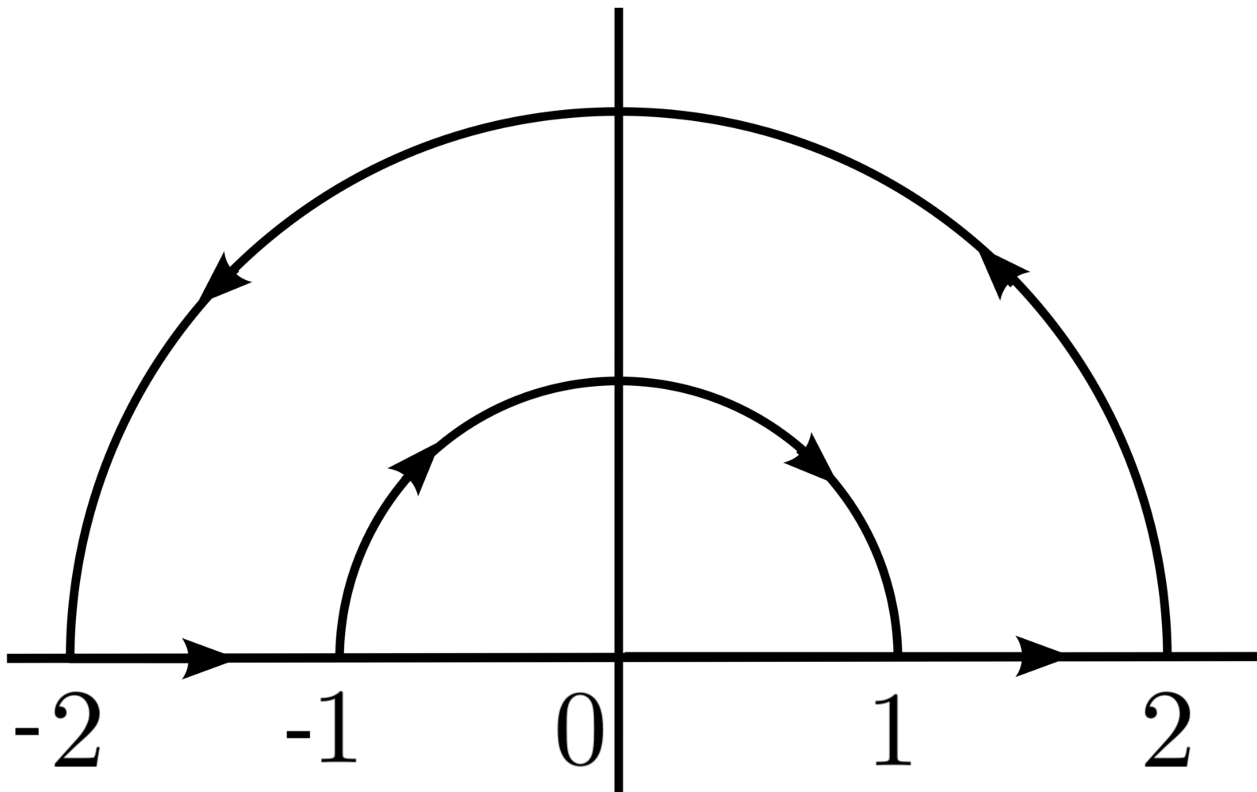
\includegraphics{7.png}
\end{center}


$(  \mathbf{5.5})  $ \ Calcular \ $\underset{\left\vert
z-a\right\vert =r}{%
%TCIMACRO{\dint }%
%BeginExpansion
{\displaystyle\int}
%EndExpansion
}(  z-a)  ^{m}dz$ \ \ $,$ \ \ $m\in%
%TCIMACRO{\U{2115} }%
%BeginExpansion
\mathbb{N}
%EndExpansion
^{\ast}$ $,$ \ $a\in$ \ e \ $r>0.$

\bigskip

No exercício seguinte introduzimos o conceito de componente conexa de

uma parte aberta de $\Omega\subset%
%TCIMACRO{\U{2102} }%
%BeginExpansion
\mathbb{C}
%EndExpansion
$ que é fundamental para a compreensão do

que segue (este conceito já foi usado no Teorema 5.2).

\bigskip

$(  \mathbf{5.6})  $ \ $(  a)  $ \ Provar que se
$(  \Omega_{\lambda})  _{\lambda\in\Lambda}$ é uma família
de abertos conexos não

vazios de $%
%TCIMACRO{\U{2102} }%
%BeginExpansion
\mathbb{C}
%EndExpansion
$ tal que \textsc{I}$:=\underset{\lambda\in\Lambda}{%
%TCIMACRO{\dbigcap }%
%BeginExpansion
{\displaystyle\bigcap}
%EndExpansion
}\Omega_{\lambda}\neq\varnothing$ \ então $\Omega:=\underset{\lambda
\in\Lambda}{%
%TCIMACRO{\dbigcup }%
%BeginExpansion
{\displaystyle\bigcup}
%EndExpansion
}\Omega_{\lambda}$ \ é um aberto conexo.

\textbf{(}\textit{Sugestão:} dados $z_{1},z_{2}\in\Omega$ arbitrários,
mostrar que $z_{1}$ e $z_{2}$ podem ser

unidos por um caminho em $\Omega$ passando por um ponto $\zeta\in$
\textsc{I}\textbf{);}

$(  b)  $ \ Seja $\Omega$ um aberto não vazio de $%
%TCIMACRO{\U{2102} }%
%BeginExpansion
\mathbb{C}
%EndExpansion
$ e para cada $z\in\Omega$ seja $C(  z)  $ a reunião

de todos os abertos conexos $V$ tais que $z\in V\subset\Omega.$ Provar que o conjunto

$C(  z)  $ é o maior aberto conexo contido em $\Omega$ que
contém $z$ (este conjunto

$C(  z)  $ é chamado \textit{componente conexa de }$z$
\textit{em }$\Omega);$ \ \ \ \ 

$(  c)  $ \ \ Prove que se $z_{1},z_{2}$\ $\in\Omega$ então
$C(  z_{1})  =C(  z_{2})  $ ou $C(  z_{1})
\cap C(  z_{2})  =\varnothing;$

deduzir que a relação $\sim$ sobre $\Omega$ definida por $z_{1}\sim
z_{2}\iff C(  z_{1})  =C(  z_{2})  $

é uma relação de equivalência;

$(  d)  $ \ Prove que todo aberto não vazio $\Omega$ se escreve
de forma única como

reunião de uma família $\ (  \Omega_{\lambda})
_{\lambda\in\Lambda}$ de abertos conexos não vazios dois a dois

disjuntos \textbf{(}\textit{Sugestão:} \ tomar como família $(
\Omega_{\lambda})  _{\lambda\in\Lambda}$ a família das classes de

equivalência de$(  c)  $\textbf{)}. Neste caso a família
$(  \Omega_{\lambda})  _{\lambda\in\Lambda}$ é dita \textit{a
família das }

\textit{componentes conexas de }$\Omega$ e dizemos que $\Omega_{\lambda}$
é uma \textit{componente conexa }

\textit{de }$\Omega$ para cada $\lambda\in\Lambda;$

$(  e)  $ \ Se $(  \Omega_{\lambda})  _{\lambda
\in\Lambda}$ é a família das componentes conexas de um aberto não vazio

$\Omega\subset%
%TCIMACRO{\U{2102} }%
%BeginExpansion
\mathbb{C}
%EndExpansion
,$ prove que $\Lambda$ é no máximo enumerável \textbf{(}%
\textit{Sugestão}: usar o exerc. 4.11

$(  a)  $\textbf{). }Mostre com exemplos que para cada $m$ $\in%
%TCIMACRO{\U{2115} }%
%BeginExpansion
\mathbb{N}
%EndExpansion
,$ $m\geq1$ existe um aberto

com exatamente $m$ componentes conexas;

$(  f)  $ \ Se $W$ é uma parte aberta conexa não vazia de
um aberto $\Omega$ de $%
%TCIMACRO{\U{2102} }%
%BeginExpansion
\mathbb{C}
%EndExpansion
,$ então

$W$ está contido numa componente conexa de $\Omega.$

\bigskip

$(  \mathbf{5.7})  $ \ Seja $\alpha\in%
%TCIMACRO{\U{2102} }%
%BeginExpansion
\mathbb{C}
%EndExpansion
,$ $\left\vert \alpha\right\vert \neq1.$ Calcule \ \textsc{I}$=\underset
{0}{\overset{}{%
%TCIMACRO{\dint ^{2\pi}}%
%BeginExpansion
{\displaystyle\int^{2\pi}}
%EndExpansion
}}%
%TCIMACRO{\QDABOVE{1pt}{dt}{1-2\alpha\cos t+\alpha^{2}}}%
%BeginExpansion
\genfrac{}{}{1pt}{0}{dt}{1-2\alpha\cos t+\alpha^{2}}%
%EndExpansion
$ \ \ integrando \ a

função \ \ $%
%TCIMACRO{\QDABOVE{1pt}{1}{(  z-\alpha)  (  z-\alpha
%^{-1})  }}%
%BeginExpansion
\genfrac{}{}{1pt}{0}{1}{(  z-\alpha)  (  z-\alpha^{-1})
}%
%EndExpansion
$ \ \ sobre o círculo unitário.

\bigskip

$(  \mathbf{5.8})  $ \ Calcular \ \ $\underset{\left\vert
z\right\vert =1}{%
%TCIMACRO{\dint }%
%BeginExpansion
{\displaystyle\int}
%EndExpansion
}%
%TCIMACRO{\QDABOVE{1pt}{e^{z}}{z}}%
%BeginExpansion
\genfrac{}{}{1pt}{0}{e^{z}}{z}%
%EndExpansion
dz$ \ .

\bigskip

$(  \mathbf{5.9})  $ \ Seja $f\in\mathcal{H}(
%TCIMACRO{\U{2102} }%
%BeginExpansion
\mathbb{C}
%EndExpansion
)  $ e suponhamos que \ $f(  z)  =\underset{\left\vert
\lambda\right\vert =1}{%
%TCIMACRO{\dint }%
%BeginExpansion
{\displaystyle\int}
%EndExpansion
}%
%TCIMACRO{\QDABOVE{1pt}{\lambda^{2}e^{\lambda}}{\lambda-z}}%
%BeginExpansion
\genfrac{}{}{1pt}{0}{\lambda^{2}e^{\lambda}}{\lambda-z}%
%EndExpansion
d\lambda,$ \ para cada

$z\in D_{1}(  0)  .$ Calcular $f(  1)  .$

\bigskip

$(  \mathbf{5.10})  $ \ Seja $%
%TCIMACRO{\dsum }%
%BeginExpansion
{\displaystyle\sum}
%EndExpansion
c_{m}(  z-\zeta)  ^{m} $ uma série de potências em volta de
$\xi$ de raio de

convergência $\rho>0$ e $f:z\in D_{\rho}(  \zeta)  \longmapsto%
%TCIMACRO{\dsum }%
%BeginExpansion
{\displaystyle\sum}
%EndExpansion
c_{m}(  z-\zeta)  ^{m}\in%
%TCIMACRO{\U{2102} }%
%BeginExpansion
\mathbb{C}
%EndExpansion
.$ Seja $\xi\in D_{\rho}(  \zeta)  $

e $r=\left\vert \xi-\zeta\right\vert :$

$(  a)  $ \ Prove que $\ f\in\mathcal{A}(  D_{\rho}(
\zeta)  )  $ \ [\textit{Sugestão:} usar Corol. 4.7 e Teor. 5.9];

$(  b)  $ \ Prove que \ $\forall$ \ $k\in%
%TCIMACRO{\U{2115} }%
%BeginExpansion
\mathbb{N}
%EndExpansion
$ \ \ temos $f^{(  k)  }(  z)  =\underset{m\geq k}{%
%TCIMACRO{\dsum }%
%BeginExpansion
{\displaystyle\sum}
%EndExpansion
}%
%TCIMACRO{\QDABOVE{1pt}{f^{(  m)  }(  \zeta)  }{(
%m-k)  !}}%
%BeginExpansion
\genfrac{}{}{1pt}{0}{f^{(  m)  }(  \zeta)  }{(
m-k)  !}%
%EndExpansion
(  z-\zeta)  ^{m-k}$ \ \ 

$\forall$ \ $z\in D_{\rho}(  \zeta)  $ \ \ [\textit{Sugestão:}
Corol. 4.8];

$(  c)  $ \ Prove que \ \ \ $f(  z)  =\underset{k\geq0}{%
%TCIMACRO{\dsum }%
%BeginExpansion
{\displaystyle\sum}
%EndExpansion
}%
%TCIMACRO{\QDABOVE{1pt}{1}{k!}}%
%BeginExpansion
\genfrac{}{}{1pt}{0}{1}{k!}%
%EndExpansion
\left[  \underset{m\geq k}{%
%TCIMACRO{\dsum }%
%BeginExpansion
{\displaystyle\sum}
%EndExpansion
}%
%TCIMACRO{\QDABOVE{1pt}{f^{(  m)  }(  \zeta)  }{(
%m-k)  !}}%
%BeginExpansion
\genfrac{}{}{1pt}{0}{f^{(  m)  }(  \zeta)  }{(
m-k)  !}%
%EndExpansion
(  \xi-\zeta)  ^{m-k}\right]  (  z-\xi)  ^{k}$ ,\ \ \ \ \ \ \ \ \ \ \ \ \ \ \ \ \ \ 

$\forall$ \ \ $z\in D_{\rho-r}(  \xi)  .$

\bigskip

$(  \mathbf{5.11})  $ \ Sejam $f\in\mathcal{H}(
%TCIMACRO{\U{2102} }%
%BeginExpansion
\mathbb{C}
%EndExpansion
)  $ e suponhamos que existem três constantes reais

positivas $A,B$ e $\alpha$ tais que

$(  \ast)  $
\ \ \ \ \ \ \ \ \ \ \ \ \ \ \ \ \ \ \ \ \ \ \ $\left\vert f(  z)
\right\vert \leq A+B\left\vert z\right\vert ^{\alpha}$ \ \ $\forall$ \ $z\in%
%TCIMACRO{\U{2102} }%
%BeginExpansion
\mathbb{C}
%EndExpansion
$

Provar que $f$ é um polinômio e que $\partial f\leq$\textbf{[[}%
$\alpha$\textbf{]] (}\textit{Sugestão}\textbf{:\ }Pelo Corol. 4.11

temos \ \ $f(  z)  =%
%TCIMACRO{\dsum }%
%BeginExpansion
{\displaystyle\sum}
%EndExpansion
(  m!)  ^{-1}f^{(  m)  }(  0)  z^{m}$
\ \ $\forall$ \ $z\in%
%TCIMACRO{\U{2102} }%
%BeginExpansion
\mathbb{C}
%EndExpansion
,$ entào basta provar que

$f^{(  n)  }(  0)  =0$ \ sempre que $n>m=$[[$\alpha$]],
o que se faz usando $(  \ast)  $ e as desigual-

dades de Cauchy). \ \ \ 

\bigskip

$(  \mathbf{5.12})  $ \ Sejam $f$ e $g$ duas funções
inteiras tais que \ $\left\vert f(  z)  \right\vert \leq\left\vert
g(  z)  \right\vert $ \ \ $\forall$ \ $z\in%
%TCIMACRO{\U{2102} }%
%BeginExpansion
\mathbb{C}
%EndExpansion
$

$(  a)  $ \ Prove que se $g(  z)  \neq0$ para cada $z\in%
%TCIMACRO{\U{2102} }%
%BeginExpansion
\mathbb{C}
%EndExpansion
,$ então existe $\ c\in%
%TCIMACRO{\U{2102} }%
%BeginExpansion
\mathbb{C}
%EndExpansion
$ \ tal que

$f=cg.$

$(  b)  $\bigskip\ \ Deduzir que para cada polinômio $p\in%
%TCIMACRO{\U{2102} }%
%BeginExpansion
\mathbb{C}
%EndExpansion
\left[  Z\right]  $, existe $\alpha\in%
%TCIMACRO{\U{2102} }%
%BeginExpansion
\mathbb{C}
%EndExpansion
$ tal que

$\left\vert p(  \alpha)  \right\vert >\left\vert e^{\alpha
}\right\vert ;$

$(  c)  $ \ Tente provar a asserção $(  a)  $
sem nenhuma hipótese sobre os zeros de $g.$

\bigskip

$(  \mathbf{5.13})  $ \ Sejam $\Omega$ um aberto de $%
%TCIMACRO{\U{2102} }%
%BeginExpansion
\mathbb{C}
%EndExpansion
$ tal que $\overline{D}_{1}(  0)  \subset\Omega,$ $f\in
\mathcal{H}(  \Omega)  $ e suponhamos

que $\ \ (  1%
%TCIMACRO{\U{ba}}%
%BeginExpansion
{{}^o}%
%EndExpansion
)  $ \ $f(  0)  =1$ \ \ $;$ \ \ \ \ $(  2%
%TCIMACRO{\U{ba}}%
%BeginExpansion
{{}^o}%
%EndExpansion
)  $ \ $\left\vert f(  z)  \right\vert >2$ \ sempre que
$\left\vert z\right\vert =1.$ Pode $f$ \ \ ter \ 

zeros em $D_{1}(  0)  ?$

\bigskip

$(  \mathbf{5.14})  $ \ Sejam $\Omega$ um aberto não vazio de $%
%TCIMACRO{\U{2102} }%
%BeginExpansion
\mathbb{C}
%EndExpansion
$ e $g\in\mathcal{C}(  \Omega;\mathbb{K})  .$ Diz-se que $g$ tem

a \textit{propriedade da média em }$\Omega$ se para cada $\overline{D}%
_{r}(  a)  \subset\Omega$ tivermos

\ \ \ \ \ \ \ \ \ \ \ \ \ \ \ \ \ \ \ \ \ \ \ \ \ \ \ \ \ \ \ $g(
a)  =%
%TCIMACRO{\QDABOVE{1pt}{1}{2\pi}}%
%BeginExpansion
\genfrac{}{}{1pt}{0}{1}{2\pi}%
%EndExpansion
\underset{0}{%
%TCIMACRO{\dint }%
%BeginExpansion
{\displaystyle\int}
%EndExpansion
}^{2\pi}g(  a+re^{it})  dt$

$\bigskip$

$(  a)  $ \ Verifique que toda $f\in\mathcal{H}(
\Omega)  $ tem a propriedade da média em $\Omega;$

$(  b)  $ \ Se $g\in\mathcal{C}(  \Omega;%
%TCIMACRO{\U{2102} }%
%BeginExpansion
\mathbb{C}
%EndExpansion
)  $ então $g$ possui a propriedade da média em $\Omega$ se e
só se

$\operatorname{Re}(  g)  $ e \textsc{I}m$(  g)  $
têm propriedade da média em $\Omega;$

$(  c)  $ \ Sejam $\zeta\in%
%TCIMACRO{\U{2102} }%
%BeginExpansion
\mathbb{C}
%EndExpansion
$, $\rho>0$ e $f\in\mathcal{C}(  D_{\rho}(  \zeta)
;\mathbb{K})  $ tal que \ $(  1%
%TCIMACRO{\U{ba}}%
%BeginExpansion
{{}^o}%
%EndExpansion
)  $ \ $f$ \ possui a

propriedade da média em $D_{\rho}(  \zeta)  ;$ \ \ $(  2%
%TCIMACRO{\U{ba}}%
%BeginExpansion
{{}^o}%
%EndExpansion
)  $ \ $\left\vert f(  z)  \right\vert \leq\left\vert
f(  \zeta)  \right\vert $ \ para cada

$z\in D_{\rho}(  \zeta)  .$ Provar que $f$ é constante em
$D_{\rho}(  \zeta)  $ \ \textbf{[}\textit{Sugestão}: \ adaptar\ a

prova do Lema 5.14; no caso $\mathbb{K=%
%TCIMACRO{\U{2102} }%
%BeginExpansion
\mathbb{C}
%EndExpansion
}$ observar que é o mesmo raciocínio

usado para provar $(  5.14.3)  ,$mas trabalhando com a parte
imaginária em

vez da parte real, implica \textsc{I}m$(
%TCIMACRO{\QDABOVE{1pt}{f(  z)  }{f(  \zeta)  }}%
%BeginExpansion
\genfrac{}{}{1pt}{0}{f(  z)  }{f(  \zeta)  }%
%EndExpansion
)  =0$ em $D_{\rho}(  \zeta)  $\textbf{] \ (}%
\textit{Observação}: é

possível provar que $g\in\mathcal{C}(  \Omega;\mathbb{K})  $
tem a propriedade da média em $\Omega$ se e

só se $g\in Har(  \Omega;\mathbb{K})  ;$ ver por exemplo
\cite{Ca}, "Fonctions Analytiques

d'une ou plusieurs variables complexas " Ch. \textsc{IV}, \S 3 e \S 4.)

\bigskip

$(  \mathbf{5.15})  $ \ Seja $g_{m}:D_{1}(  0)
\rightarrow%
%TCIMACRO{\U{2102} }%
%BeginExpansion
\mathbb{C}
%EndExpansion
$ a função definida por $g_{m}(  z)  =z^{m},$ $m\in%
%TCIMACRO{\U{2115} }%
%BeginExpansion
\mathbb{N}
%EndExpansion
.$

Prove que a sequência $(  g_{m})  $ converge uniformemente
sobre os compactos

$D_{1}(  0)  $ para a função nula sobre $D_{1}(
0)  ,$ porém $(  g_{m})  $ não converge uniforme-

mente para a função nula em $D_{1}(  0)  .$

\bigskip

$(  \mathbf{5.16})  $ \ Sejam $\Omega$ um aberto não vazio e
$(  f_{m})  _{m\in%
%TCIMACRO{\U{2115} }%
%BeginExpansion
\mathbb{N}
%EndExpansion
}$ uma sequência em $\mathcal{C}(  \Omega;\mathbb{K})  $

tal que $(  f_{m})  $ converge uniformemente sobre os compactos de
$\Omega$ para uma

função $f:\Omega\rightarrow\mathbb{K}.$

Prove que $f\in\mathcal{C}(  \Omega;\mathbb{K})  $ \ \textbf{[}%
\textit{Sugestão}: A desigualdade evidente

\ \ \ \ $\left\vert f(  z)  -f(  \zeta)  \right\vert
\leq\left\vert f(  z)  -f_{m}(  z)  \right\vert
+\left\vert f_{m}(  z)  -f_{m}(  \zeta)  \right\vert
+\left\vert f_{m}(  \zeta)  -f(  \zeta)  \right\vert ,$

vale para todo $z,\zeta\in\Omega$ e todo $m\in%
%TCIMACRO{\U{2115} }%
%BeginExpansion
\mathbb{N}
%EndExpansion
;$ usar a convergência uniforme de $(  f_{m})  $

para majorar a 1%
%TCIMACRO{\U{aa} }%
%BeginExpansion
${{}^a}$
%EndExpansion
e a 3%
%TCIMACRO{\U{aa} }%
%BeginExpansion
${{}^a}$
%EndExpansion
parcela e fixar $m$, com este valor fixo de $m$ majorar

a 2%
%TCIMACRO{\U{aa} }%
%BeginExpansion
${{}^a}$
%EndExpansion
parcela.\textbf{]}

\bigskip

$(  \mathbf{5.17})  $ \ Sejam \ $\Omega:=\left\{  z\in%
%TCIMACRO{\U{2102} }%
%BeginExpansion
\mathbb{C}
%EndExpansion
\text{ }|\text{ }\left\vert
%TCIMACRO{\QDABOVE{1pt}{z}{z+1}}%
%BeginExpansion
\genfrac{}{}{1pt}{0}{z}{z+1}%
%EndExpansion
\right\vert <1\right\}  $ \ e \ seja

\ \ \ \ \ \ \ \ \ \ \ \ \ \ \ \ \ \ \ \ \ \ \ \ \ \ \ \ $f:z\in\Omega
\longmapsto\underset{m\geq0}{%
%TCIMACRO{\dsum }%
%BeginExpansion
{\displaystyle\sum}
%EndExpansion
}(
%TCIMACRO{\QDABOVE{1pt}{z}{z+1}}%
%BeginExpansion
\genfrac{}{}{1pt}{0}{z}{z+1}%
%EndExpansion
)  ^{m}\in%
%TCIMACRO{\U{2102} }%
%BeginExpansion
\mathbb{C}
%EndExpansion
$

Prove que $f\in\mathcal{H}(  \Omega)  $ \ \ \textbf{[}%
\textit{Sugestão:} ver Exemplo que segue a Prop. 3.5\textbf{]}

\bigskip

$(  \mathbf{5.18})  $ \ Existe ou não uma sequência de
polinômios que converge

uniformemente em $D_{1}(  0)  $ para $f(  z)
=\overline{z}.$ Justifique sua resposta.

\bigskip

\bigskip$(  \mathbf{5.19})  $ \ Calcular as seguintes integrais:

$\bigskip$

$(  a)  $ \ \ $\underset{\left\vert z\right\vert =1}{%
%TCIMACRO{\dint }%
%BeginExpansion
{\displaystyle\int}
%EndExpansion
}%
%TCIMACRO{\QDABOVE{1pt}{1+senz}{z}}%
%BeginExpansion
\genfrac{}{}{1pt}{0}{1+senz}{z}%
%EndExpansion
dz$ \ \ \ \ \ \ \ \ \ (aplicar o Teor. 5.8 à função

\ \ \ \ \ \ \ \ \ \ \ \ \ \ \ \ \ \ \ \ \ \ \ \ \ \ \ \ \ \ \ \ \ \ \ \ \ \ \ \ \ \ $f(
z)  :=1+senz$ \ $\forall$\ $z\in%
%TCIMACRO{\U{2102} }%
%BeginExpansion
\mathbb{C}
%EndExpansion
$)

$\bigskip$

$(  b)  $ $\underset{\left\vert z\right\vert =1}{%
%TCIMACRO{\dint }%
%BeginExpansion
{\displaystyle\int}
%EndExpansion
}%
%TCIMACRO{\QDABOVE{1pt}{\cos z}{z}}%
%BeginExpansion
\genfrac{}{}{1pt}{0}{\cos z}{z}%
%EndExpansion
dz$ \ \ \ \ \ \ \ \ \ \ \ \ \ \ \ \ \ (mesma coisa que $(  a)  $)

$(  c)  $ \ $\underset{\left\vert z\right\vert =1}{%
%TCIMACRO{\dint }%
%BeginExpansion
{\displaystyle\int}
%EndExpansion
}%
%TCIMACRO{\QDABOVE{1pt}{senz}{z}}%
%BeginExpansion
\genfrac{}{}{1pt}{0}{senz}{z}%
%EndExpansion
dz$ \ \ \ \ \ \ \ \ \ \ \ \ \ \ \ \ \ (mesma coisa que $(  a)  $)

$(  d)  $ \ $\underset{\left\vert z\right\vert =1}{%
%TCIMACRO{\dint }%
%BeginExpansion
{\displaystyle\int}
%EndExpansion
}%
%TCIMACRO{\QDABOVE{1pt}{e^{iz}}{z^{2}}}%
%BeginExpansion
\genfrac{}{}{1pt}{0}{e^{iz}}{z^{2}}%
%EndExpansion
dz$ \ \ \ \ \ \ \ \ \ \ \ \ \ \ \ \ \ \ \ (aplicar o Corol. 5.10 à função

\ \ \ \ \ \ \ \ \ \ \ \ \ \ \ \ \ \ \ \ \ \ \ \ \ \ \ \ \ \ \ \ \ \ \ \ \ \ \ \ \ $f(
z)  :=e^{iz}$ \ $\forall$ \ $z\in%
%TCIMACRO{\U{2102} }%
%BeginExpansion
\mathbb{C}
%EndExpansion
$)

$\bigskip$

$(  e)  $ \ $\underset{\left\vert z\right\vert =1}{%
%TCIMACRO{\dint }%
%BeginExpansion
{\displaystyle\int}
%EndExpansion
}%
%TCIMACRO{\QDABOVE{1pt}{e^{z}-e^{-z}}{z^{m}}}%
%BeginExpansion
\genfrac{}{}{1pt}{0}{e^{z}-e^{-z}}{z^{m}}%
%EndExpansion
dz$ \ \ \ \ \ \ \ \ \ (aplicar o Corol. 5.10 a $f^{(  m-1)
}(  0)  $ sendo

\ \ \ \ \ \ \ \ \ \ \ \ \ \ \ \ \ \ \ \ \ \ \ \ \ \ \ \ \ \ \ \ \ \ \ \ \ \ \ \ \ \ $f(
z)  :=e^{z}-e^{-z}$ \ \ $\forall$ \ $z\in%
%TCIMACRO{\U{2102} }%
%BeginExpansion
\mathbb{C}
%EndExpansion
$)

\bigskip

$(  \mathbf{5.20})  $ \ Seja $\Omega$ um aberto conexo contendo
$\overline{D}_{2}(  0)  $ e seja $f\in\mathcal{H}(
\Omega)  $ tal que

\ \ \ \ \ \ \ \ \ \ \ \ \ \ \ \ \ \ 

$\ \ \ \ \ \ \ \ \ \ \ \ \ \ \ \ \ \ \ \ \ \ \ \ \ f(  z)
=\underset{\left\vert \lambda\right\vert =1}{%
%TCIMACRO{\dint }%
%BeginExpansion
{\displaystyle\int}
%EndExpansion
}%
%TCIMACRO{\QDABOVE{1pt}{\lambda^{3}\cos\lambda d\lambda}{\lambda-z}}%
%BeginExpansion
\genfrac{}{}{1pt}{0}{\lambda^{3}\cos\lambda d\lambda}{\lambda-z}%
%EndExpansion
d\lambda$ \ \ \ \ para cada $z\in D_{1}(  0)  .$

Calcular \ $f(  2i)  .$

\bigskip

$(  \mathbf{5.21})  $ \ Sejam $r$ \ um número real positivo, e
para cada $m\in%
%TCIMACRO{\U{2115} }%
%BeginExpansion
\mathbb{N}
%EndExpansion
$ \ seja

$\gamma_{m}:t\in\left[  0,2\pi\right]  \longmapsto r_{m}e^{it}\in%
%TCIMACRO{\U{2102} }%
%BeginExpansion
\mathbb{C}
%EndExpansion
$ o círculo orientado positivamente de centro $0$

e raio $r_{m},$ onde $r_{0}:=r$ \ \ e $\ r_{m}:=(  1-1/m)  r$ \ se
$m\geq1$

$(  a)  $ \ Prove que se $f\in\mathcal{C}(  \overline{D_{r}%
}(  0)  )  $ então

\ \ \ \ \ \ \ \ \ \ \ \ \ \ \ \ \ \ \ \ \ \ \ \ \ \ \ \ \ \ \ \ \ \ \ 

\ \ \ \ \ \ \ \ \ \ \ \ \ \ \ \ \ \ \ \ \ \ \ \ \ \ \ \ \ \ \ \ $\underset
{\gamma}{%
%TCIMACRO{\dint }%
%BeginExpansion
{\displaystyle\int}
%EndExpansion
}f(  z)  dz=\underset{m\rightarrow\infty}{\lim}\underset{\gamma
_{m}}{%
%TCIMACRO{\dint }%
%BeginExpansion
{\displaystyle\int}
%EndExpansion
}f(  z)  dz$

$(  b)  $ \ Deduzir que se $f\in\mathcal{C}(  \overline{D}%
_{r}(  0)  )  \cap\mathcal{H}(  D_{r}(  0)
)  $ \ \ então

\ \ \ \ \ \ \ \ \ \ \ \ \ \ \ \ \ \ \ \ \ \ \ \ 

$\ \ \ \ \ \ \ \ \ \ \ \ \ \ \ \ \ \ \ \ \ \ \ \ \ \ \ \ \ \ f(
z)  =%
%TCIMACRO{\QDABOVE{1pt}{1}{2\pi i}}%
%BeginExpansion
\genfrac{}{}{1pt}{0}{1}{2\pi i}%
%EndExpansion
\underset{\left\vert \lambda\right\vert =r}{%
%TCIMACRO{\dint }%
%BeginExpansion
{\displaystyle\int}
%EndExpansion
}%
%TCIMACRO{\QDABOVE{1pt}{f(  \lambda)  d\lambda}{\lambda-z}}%
%BeginExpansion
\genfrac{}{}{1pt}{0}{f(  \lambda)  d\lambda}{\lambda-z}%
%EndExpansion
,$ \ \ sempre $\left\vert z\right\vert <r.$

\bigskip

$(  \mathbf{5.22})  $ \ Sejam $f\in\mathcal{H}(
%TCIMACRO{\U{2102} }%
%BeginExpansion
\mathbb{C}
%EndExpansion
)  $ e $a\in%
%TCIMACRO{\U{2102} }%
%BeginExpansion
\mathbb{C}
%EndExpansion
.$

$(  a)  $ \ Prove que as derivadas sucessivas de $f$ no ponto $a$
não podem satisfazer

desigualdades do tipo:

\ \ \ \ \ \ \ \ \ \ \ \ \ \ \ \ \ \ \ \ \ \ \ \ \ \ \ \ \ \ \ \ \ $\left\vert
f^{(  m)  }(  a)  \right\vert >m!m^{m}$ \ \ \ $\forall$
\ $m\in%
%TCIMACRO{\U{2115} }%
%BeginExpansion
\mathbb{N}
%EndExpansion
$

$(  b)  $ Formular um resultado do tipo $(  a)  $ que
seja melhor que $(  a)  .$ \ \textbf{[}\textit{Sugestão}:

para $(  a)  $ e $(  b)  :$ Usar o Corol.
5.11\textbf{].}

\bigskip

$(  \mathbf{5.23})  $ \ (Ver comentário que segue o enunciado
do Lema 5.6) \ Seja $\Omega$ um

aberto não vazio de $%
%TCIMACRO{\U{2102} }%
%BeginExpansion
\mathbb{C}
%EndExpansion
,$ seja $p\in\Omega$ e seja $f\in\mathcal{C}(  \Omega)  $ tal que
$f\in\mathcal{H}(  \Omega\backslash\left\{  p\right\}  )  .$

Prove que $f\in\mathcal{H}(  \Omega)  .$ [\textit{Sugestão}:
\ Usar o Lema 5.6 e o Teor. 5.17].

\bigskip

\textbf{(5.24) \ }Se $f=u+iv\in\mathcal{H}(  \Omega)  $, onde
$u=\operatorname{Re}(  f)  $ e $v=$\textsc{I}m$(  f)  ,$ então

$f\in\mathcal{C}^{\infty}(  \Omega)  $ (isto é, $f$ é
infinitamente $%
%TCIMACRO{\U{211d} }%
%BeginExpansion
\mathbb{R}
%EndExpansion
$-diferenciável em $\Omega$)

\bigskip

\textbf{[Sugestão: \ }Comecemos lembrando as expressões de $f^{\prime
}$ em função das

derivadas parciais de $u$ e $v$ (ver Obs. logo após o fim da prova do
Teor. 2.3)

\bigskip

(1) \ \ \ \ \ \ \ \ \ \ \ \ $f^{\prime}=u_{x}+iv_{x}=v_{y}-iu_{y}=u_{x}%
-iu_{y}=v_{y}+iv_{x}$

\bigskip

De \ $f\in\mathcal{H}(  \Omega)  =\mathcal{A}(  \Omega)
$ segue $f^{\prime}\in\mathcal{A}(  \Omega)  \subset\mathcal{C}%
(  \Omega)  $ portanto por (1) resulta

que $u_{x},v_{x},u_{y}$ e $v_{y}$ são contínuas em $\Omega$ logo

\bigskip

(1$^{\prime}$) \ \ \ \ \ \ \ \ \ \ \ \ \ \ \ \ \ \ \ \ \ \ \ \ \ $f\in
\mathcal{C}^{1}(  \Omega)  $

\bigskip

Observe a seguir que $f^{\prime\prime}\in\mathcal{A}(  \Omega)  $ e
se aplicar (1) ao cálculo de $f^{\prime\prime}$ obtem-se

\bigskip

(2) \ \ \ \ \ \ \ \ \ \ \ \ \ \ \ \ \ \ \ \ \ \ $f^{\prime\prime}=\left\{
\begin{array}
[c]{c}%
v_{xy}-iu_{xy}=-u_{yy}-iv_{yy}=\\
u_{xx}+iv_{xx}=v_{yx}-iu_{yx}\text{ }.\text{\ \ \ }%
\end{array}
\right.  $

\bigskip

De novo, $f^{\prime\prime}\in\mathcal{A}(  \Omega)  \subset
\mathcal{C}(  \Omega)  $ logo (2) mostra que todas as derivadas de
2$^{\underline{a}}$

ordem $u$ e $v$ são contínuas em $\Omega$, isto é,

\bigskip

(2$^{\prime}$)
\ \ \ \ \ \ \ \ \ \ \ \ \ \ \ \ \ \ \ \ \ \ \ \ \ \ \ \ \ \ \ \ $f\in
\mathcal{C}^{2}(  \Omega)  .$

\bigskip

A obtenção acima \ de (1$^{\prime}$) e (2$^{\prime}$) sugerem o
próximo passo que consiste em

provar o seguinte:

\bigskip

\textbf{Lema \ }Sejam $m\in%
%TCIMACRO{\U{2115} }%
%BeginExpansion
\mathbb{N}
%EndExpansion
^{\ast}$ e $(  \alpha,\beta)  \in%
%TCIMACRO{\U{2115} }%
%BeginExpansion
\mathbb{N}
%EndExpansion
\times%
%TCIMACRO{\U{2115} }%
%BeginExpansion
\mathbb{N}
%EndExpansion
$ tal que \ $\alpha+\beta=m.$ Então

\bigskip

(3) \ \ \ \ \ \ \ \ \ \ \ \ \ \ \ \ \ \ \ \ $f^{(  m)  }=\left\{
\begin{array}
[c]{c}%
\pm%
%TCIMACRO{\QDABOVE{1pt}{\partial^{m}u}{\partial x^{\alpha}\partial y^{\beta}}}%
%BeginExpansion
\genfrac{}{}{1pt}{0}{\partial^{m}u}{\partial x^{\alpha}\partial y^{\beta}}%
%EndExpansion
\pm^{\prime}i%
%TCIMACRO{\QDABOVE{1pt}{\partial^{m}v}{\partial x^{\alpha}\partial y^{\beta}}}%
%BeginExpansion
\genfrac{}{}{1pt}{0}{\partial^{m}v}{\partial x^{\alpha}\partial y^{\beta}}%
%EndExpansion
=\\
\\
\pm%
%TCIMACRO{\QDABOVE{1pt}{\partial^{m}v}{\partial x^{\alpha}\partial y^{\beta}}}%
%BeginExpansion
\genfrac{}{}{1pt}{0}{\partial^{m}v}{\partial x^{\alpha}\partial y^{\beta}}%
%EndExpansion
\pm^{\prime}i%
%TCIMACRO{\QDABOVE{1pt}{\partial^{m}u}{\partial x^{\alpha}\partial y^{\beta}}}%
%BeginExpansion
\genfrac{}{}{1pt}{0}{\partial^{m}u}{\partial x^{\alpha}\partial y^{\beta}}%
%EndExpansion
\text{ \ }%
\end{array}
\right.  $

\bigskip

onde a notação $\pm^{\prime}$ significa que $\pm$ e $\pm^{\prime}%
$são independentes.

\bigskip

\textbf{Prova do lema\ \ }Proceda por indução sobre $m.$

\bigskip

\textbf{Afirmação: \ }$f\in\mathcal{C}^{\infty}(  \Omega)
.$ Dados $m\in%
%TCIMACRO{\U{2115} }%
%BeginExpansion
\mathbb{N}
%EndExpansion
^{\ast}$ arbitrário e $(  \alpha,\beta)  \in%
%TCIMACRO{\U{2115} }%
%BeginExpansion
\mathbb{N}
%EndExpansion
\times%
%TCIMACRO{\U{2115} }%
%BeginExpansion
\mathbb{N}
%EndExpansion
$ tal

que $\alpha+\beta=m$ $,$ $%
%TCIMACRO{\QDABOVE{1pt}{\partial^{m}u}{\partial x^{\alpha}\partial y^{\beta}}}%
%BeginExpansion
\genfrac{}{}{1pt}{0}{\partial^{m}u}{\partial x^{\alpha}\partial y^{\beta}}%
%EndExpansion
$ e $%
%TCIMACRO{\QDABOVE{1pt}{\partial^{m}v}{\partial x^{\alpha}\partial y^{\beta}}}%
%BeginExpansion
\genfrac{}{}{1pt}{0}{\partial^{m}v}{\partial x^{\alpha}\partial y^{\beta}}%
%EndExpansion
$ são contínuas. De fato,

$f^{(  m)  }\in\mathcal{A}(  \Omega)  \subset
\mathcal{C}(  \Omega)  ,$ então $f^{(  m)  }$ se
escreve em algumas das 8 for-

mas (3) e então a continuidade das derivadas parciais acima segue da

continuidade de $f^{(  m)  }.$\textbf{]}

\pagebreak

% Capítulo 6

\textbf{{\fontsize{18}{18}\selectfont Capítulo 6\\\\}}

\textbf{{\fontsize{20}{20}\selectfont \ \ \ O TEOREMA DA APLICAÇÃO \\}}

\textbf{{\fontsize{20}{20}\selectfont \ \ ABERTA. INVERSÃO DE \\}}

\textbf{{\fontsize{20}{20}\selectfont \ \  FUNÇÕES ANALÍTICAS: \\}}

\textbf{{\fontsize{20}{20}\selectfont \ \  O PROBLEMA GLOBAL. \\}}

\textbf{{\fontsize{20}{20}\selectfont \ \  A FUNÇÃO LOGARITMO. \\\\\\}}

\bigskip

\textbf{Lema 6.1 \ \ }\textit{Sejam }$\Omega$ um aberto não vazio de $%
%TCIMACRO{\U{2102} }%
%BeginExpansion
\mathbb{C}
%EndExpansion
,$ $f\in\mathcal{H}(  \Omega)  $ \textit{e }$g:\Omega\times
\Omega\rightarrow%
%TCIMACRO{\U{2102} }%
%BeginExpansion
\mathbb{C}
%EndExpansion
$ \textit{\ }

\textit{a função definida por}

\ \ \ \ \ \ \ \ \ \ \ \ \ \ \ \ \ \ \ \ $g(  z,w)  :=\left\{
\begin{array}
[c]{c}%
%TCIMACRO{\QDABOVE{1pt}{f(  z)  -f(  w)  }{z-w}}%
%BeginExpansion
\genfrac{}{}{1pt}{0}{f(  z)  -f(  w)  }{z-w}%
%EndExpansion
\text{ \ },\text{ se \ }z\neq w\\
\\
f^{\prime}(  z)  \text{ \ },\text{ \ se \ }z=w\text{
\ \ \ \ \ \ \ \ }%
\end{array}
\right.  $

\textit{Então }$g\in\mathcal{C}(  \Omega\times\Omega)  .$

\bigskip



\bigskip\textbf{Prova} \ Os únicos pontos nos quais a continuidade de $g $
não é evidente são

aqueles do tipo $(  z,z)  .$Fixemos $a\in\Omega$ e $\varepsilon>0.$
Como $\ f'$ é continua em $\Omega,$



existe $r>0$ tal que

$(  6.1.1)  $ \ \ \ $z\in D_{r}(  a)  \implies\left\vert
f^{\prime}(  z)  -f^{\prime}(  a)  \right\vert
<\varepsilon$


\bigskip

Bastará provar então

\bigskip





$(  6.1.2)  $ \ \ \ $(  z,w)  \in D_{r}(  a)
\times D_{r}(  a)  \implies\left\vert g(  z,w)
-g(  a,a)  \right\vert <\varepsilon.$

% IMAGEM 19

\begin{wrapfigure}[1]{r}{0.3\textwidth}
  \begin{center}
    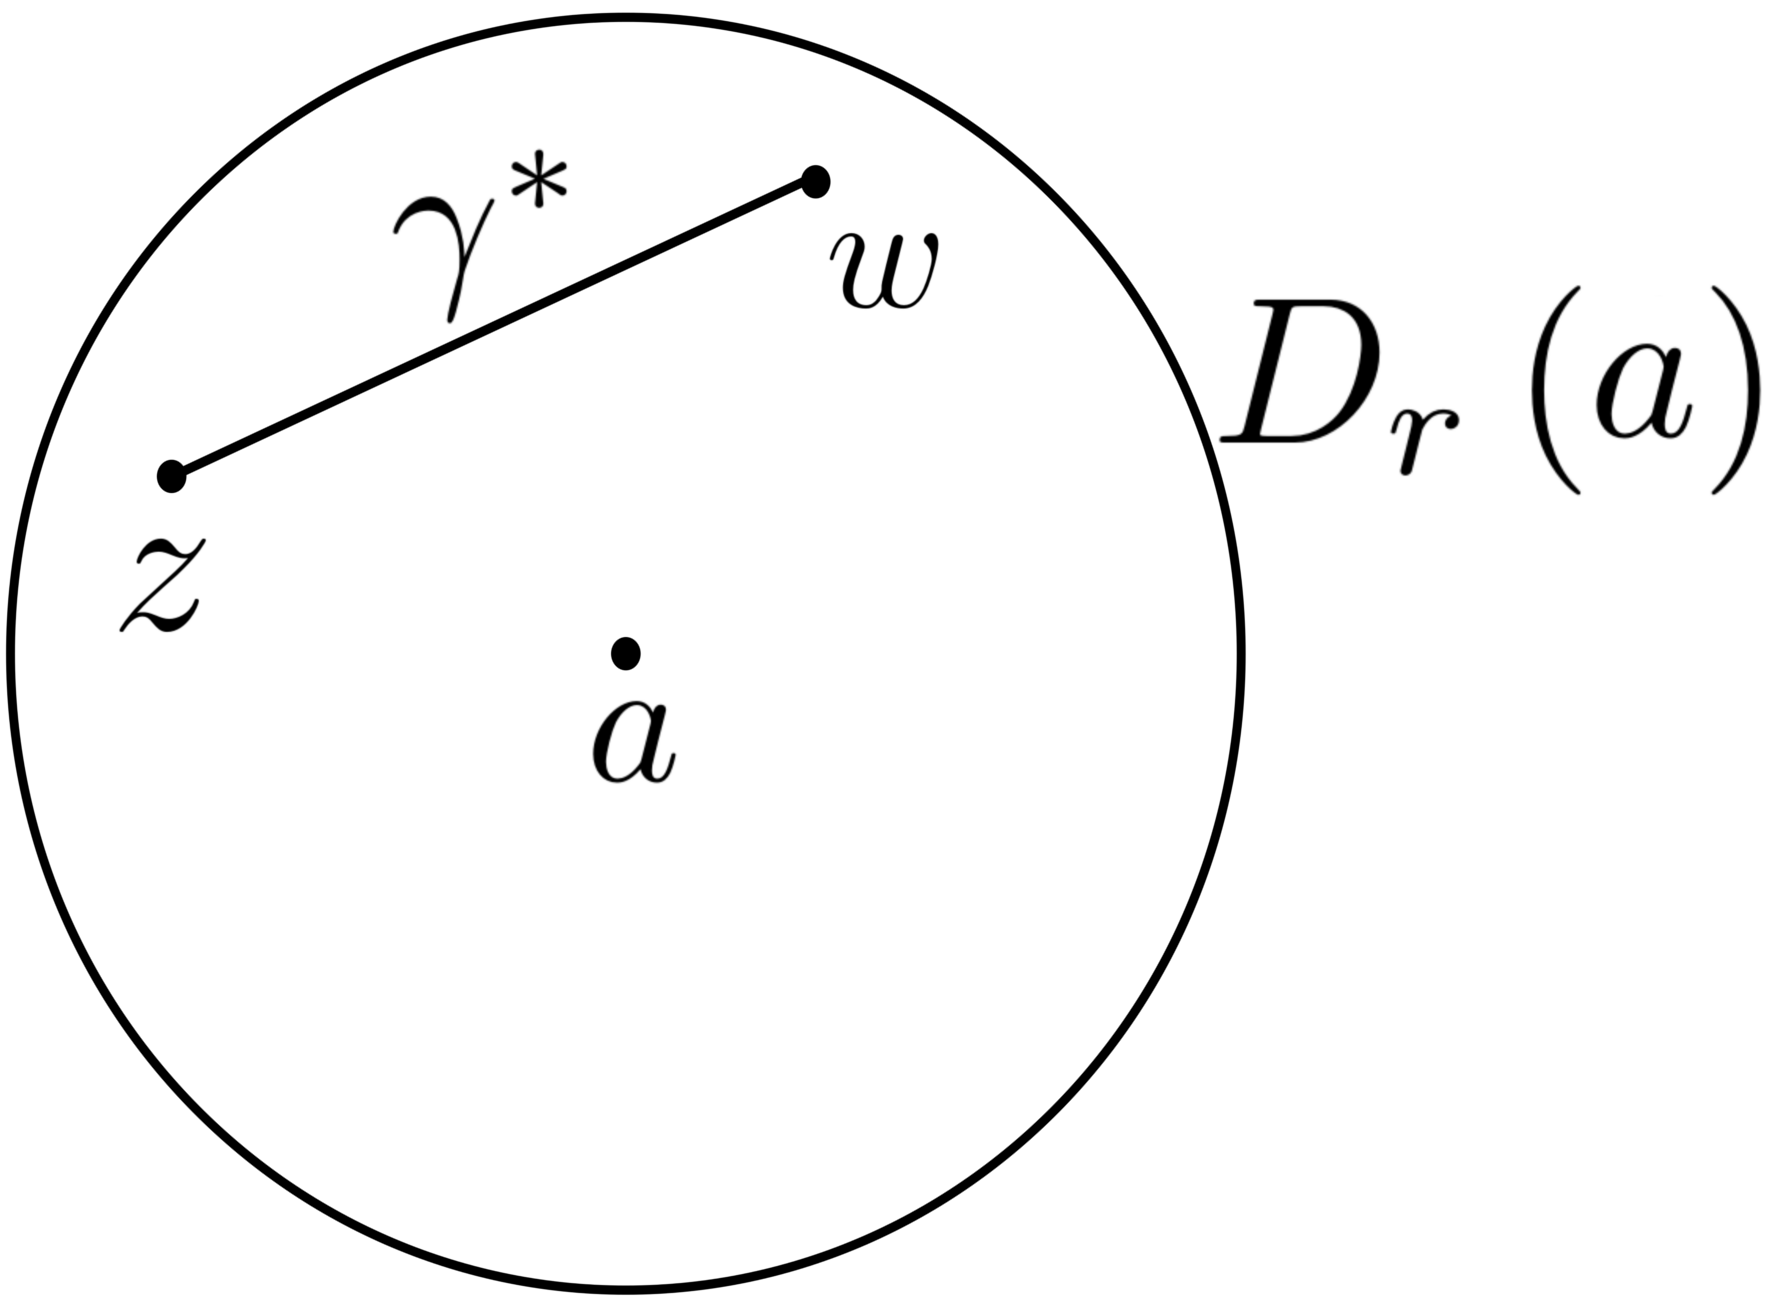
\includegraphics[width=0.3\textwidth]{19.png}
  \end{center}
\end{wrapfigure}

\bigskip

Seja $(  z,w)  \in D_{r}(  a)  \times D_{r}(
a)  $ arbitrário tal que $z\neq $

$w$ e consideremos o intervalo orientado de origem 

$z$ e extremo $w,$

$\ \gamma:t\in\left[  0,1\right]  \longmapsto(  1-t)  z+tw\in%
%TCIMACRO{\U{2102} }%
%BeginExpansion
\mathbb{C}
%EndExpansion
$.\ \ 



Como $D_{r}(  a)  $ é convexo, é claro que


\bigskip

$(  6.1.3)  $ \ \ \ $\gamma(  t)  $\ $\in D_{r}(
a)  $ para cada $t\in\left[  0,1\right]  $\ \ \ \ \ \ \ 

\bigskip

Vamos calcular $\underset{\gamma}{{\displaystyle\int}}$\ $f^{\prime}$ de duas formas (na primeira 

\bigskip

usamos que $\gamma^{\prime}(  t)  =w-z$ $\forall$ $t\in\left[  0,1\right]  $ e na segunda, o teorema fundamental 

do cálculo):

\bigskip$\underset{\gamma}{%
%TCIMACRO{\dint }%
%BeginExpansion
{\displaystyle\int}
%EndExpansion
}f^{\prime}(  z)  dz=\underset{0}{%
%TCIMACRO{\dint }%
%BeginExpansion
{\displaystyle\int}
%EndExpansion
}^{1}f^{\prime}\left[  \gamma(  t)  \right]  \gamma^{\prime}(
t)  dt=\left\{
\begin{array}
[c]{c}%
(  w-z)  \underset{0}{%
%TCIMACRO{\dint ^{1}}%
%BeginExpansion
{\displaystyle\int^{1}}
%EndExpansion
}f^{\prime}\left[  \gamma(  t)  \right]  dt\text{
\ \ \ \ \ \ \ \ \ \ \ \ \ \ \ }\\
\\
f(\gamma(  1)  )-f(  \gamma(  0)  )
=f(  w)  -f(  z)
\end{array}
\right.  $

\bigskip

em consequência, se $(  z,w)  \in D_{r}(  a)  \times
D_{r}(  a)  $ e $z\neq w$ temos

\ \ \ \ \ \ \ \ \ \ \ \ \ 

\ \ \ \ \ \ \ \ \ \ \ \ \ \ \ $(  w-z)  \underset{0}{%
%TCIMACRO{\dint }%
%BeginExpansion
{\displaystyle\int}
%EndExpansion
}^{1}f^{\prime}\left[  \gamma(  t)  \right]  dt=f(  w)
-f(  z)  $

o que implica

$\bigskip$

$g(  z,w)  =%
%TCIMACRO{\QDABOVE{1pt}{f(  z)  -f(  w)  }{z-w}}%
%BeginExpansion
\genfrac{}{}{1pt}{0}{f(  z)  -f(  w)  }{z-w}%
%EndExpansion
=\underset{0}{%
%TCIMACRO{\dint }%
%BeginExpansion
{\displaystyle\int}
%EndExpansion
}^{1}f^{\prime}\left[  \gamma(  t)  \right]  dt$ \ $,$\ se $(
z,w)  \in D_{r}(  a)  \times D_{r}(  a)  $ e
$z\neq w$

e como $g(  a,a)  =f^{\prime}(  a)  =\underset{0}{%
%TCIMACRO{\dint }%
%BeginExpansion
{\displaystyle\int}
%EndExpansion
}^{1}f^{\prime}(  a)  dt$ \ $,$ podemos escrever

$g(  z,w)  -g(  a,a)  =\left\{
\begin{array}
[c]{c}%
f^{\prime}(  z)  -f^{\prime}(  a)  \text{ \ },\text{
\ se }z=w\in D_{r}(  a)  \text{
\ \ \ \ \ \ \ \ \ \ \ \ \ \ \ \ \ \ \ \ \ \ \ \ \ \ \ \ \ \ \ \ \ \ \ }\\
\\
\underset{0}{%
%TCIMACRO{\dint }%
%BeginExpansion
{\displaystyle\int}
%EndExpansion
}^{1}\left[  f^{\prime}\left[  \gamma(  t)  \right]  -f^{\prime
}(  a)  \right]  dt,\text{ \ se \ }(  z,w)  \in
D_{r}(  a)  \times D_{r}(  a)  \text{ \ e \ }z\neq
w\text{ \ }%
\end{array}
\right.  $

\bigskip

e então, para cada $(  z,w)  \in D_{r}(  a)  \times
D_{r}(  a)  $ resulta

\bigskip$\left\vert g(  z,w)  -g(  a,a)  \right\vert
=\left\{
\begin{array}
[c]{c}%
\left\vert f^{\prime}(  z)  -f^{\prime}(  a)
\right\vert <\varepsilon\text{ \ },\text{ por }(  6.1.1)  \text{
\ \ \ \ \ \ \ \ \ \ \ \ \ \ \ \ \ \ \ \ \ \ \ \ \ \ \ \ \ \ \ \ \ \ \ \ \ \ \ \ \ \ \ \ \ \ \ \ \ \ \ \ \ \ \ \ \ \ \ \ \ \ \ \ \ \ \ \ \ \ \ \ \ \ }%
\\
\\
\left\vert \underset{0}{%
%TCIMACRO{\dint ^{1}}%
%BeginExpansion
{\displaystyle\int^{1}}
%EndExpansion
}\left[  f^{\prime}(  \gamma(  t)  )  -f^{\prime}(
a)  \right]  dt\right\vert \leq\underset{0}{%
%TCIMACRO{\dint ^{1}}%
%BeginExpansion
{\displaystyle\int^{1}}
%EndExpansion
}\left\vert f^{\prime}\left[  \gamma(  t)  \right]  -f^{\prime
}(  a)  \right\vert dt<\varepsilon\text{ \ },\text{
\ \ \ \ \ \ \ \ \ \ \ \ \ \ \ \ \ \ \ \ \ \ \ \ \ \ \ \ \ \ \ \ \ \ \ \ \ \ \ }%
\\
\text{por }(  6.1.1)  \text{ e }(  6.1.3)  \text{
};\text{
\ \ \ \ \ \ \ \ \ \ \ \ \ \ \ \ \ \ \ \ \ \ \ \ \ \ \ \ \ \ \ \ \ \ \ \ \ \ \ \ \ \ \ \ \ \ \ \ \ \ \ \ \ \ \ \ \ \ \ \ \ \ \ \ \ \ \ \ \ \ \ \ \ \ \ \ \ \ \ \ \ \ \ \ \ }%
\end{array}
\right.  $

\bigskip

o que demonstra $(  6.1.2)  .$ $\square$

\bigskip

\textbf{Teorema 6.2 \ (Teorema da função inversa, caso local)
\ }\textit{Sejam }$\Omega$\textit{\ um }

\textit{aberto não vazio de }$%
%TCIMACRO{\U{2102} }%
%BeginExpansion
\mathbb{C}
%EndExpansion
,$ $\varphi\in\mathcal{H}(  \Omega)  ,$ $z_{0}\in\Omega$\textit{\ e
suponhamos que }$\varphi^{\prime}(  z_{0})  \neq0.$\textit{\ }

\textit{Então existe }$\rho>0$ \textit{tal que }$V:=D_{\rho}(
z_{0})  \subset\Omega$ \textit{\ de modo que }

(a) \ $\varphi|V$ \ \textit{é injetora,}

(b) \ $W:=\varphi(  V)  $ \textit{\ é aberto}

(c) \ $\varphi^{-1}$ $\in\mathcal{H}(  W)  $\ \ \textit{e }%
$\varphi^{-1^{\prime}}(  w)  =%
%TCIMACRO{\QDABOVE{1pt}{1}{\varphi^{\prime}\left[  \varphi^{-1}(
%w)  \right]  }}%
%BeginExpansion
\genfrac{}{}{1pt}{0}{1}{\varphi^{\prime}\left[  \varphi^{-1}(  w)
\right]  }%
%EndExpansion
$ \ \ $\forall$ \ $w\in W$ $.$

\bigskip

\textbf{Prova \ }Consideremos a função $g$ definida por

\ \ \ \ \ \ \ \ \ \ \ \ \ \ \ \ \ 

$\ \ \ \ \ \ \ \ \ \ \ \ \ \ \ \ g(  z,w)  =\left\{
\begin{array}
[c]{c}%
%TCIMACRO{\QDABOVE{1pt}{\varphi(  z)  -\varphi(  w)
%}{z-w}}%
%BeginExpansion
\genfrac{}{}{1pt}{0}{\varphi(  z)  -\varphi(  w)  }{z-w}%
%EndExpansion
\text{ \ },\text{ \ se }z\neq w\\
\\
\varphi^{\prime}(  z)  \text{ },\text{ se }z=w\text{
\ \ \ \ \ \ \ \ \ \ \ \ \ \ }%
\end{array}
\right.  $

\bigskip

então pelo Lema 6.1, $g$ é contínua no ponto $(  z_{0}%
,z_{0})  $ e portanto para

$\varepsilon:=%
%TCIMACRO{\QDABOVE{1pt}{1}{2}}%
%BeginExpansion
\genfrac{}{}{1pt}{0}{1}{2}%
%EndExpansion
\left\vert \varphi^{\prime}(  z_{0})  \right\vert >0,$ existe
$\rho>0$ tal que $V:=D_{\rho}(  z_{0})  \subset\Omega$ \ e

\bigskip

$(  6.2.1)  $ \ \ $(  z_{1},z_{2})  \in V\times
V\implies\left\vert g(  z_{1,}z_{2})  -g(  z_{0},z_{0})
\right\vert \leq%
%TCIMACRO{\QDABOVE{1pt}{1}{2}}%
%BeginExpansion
\genfrac{}{}{1pt}{0}{1}{2}%
%EndExpansion
\left\vert \varphi^{\prime}(  z_{0})  \right\vert $.

\bigskip

Pela definição de $g$ e pela 2%
%TCIMACRO{\U{aa} }%
%BeginExpansion
${{}^a}$
%EndExpansion
propriedade triangular podemos escrever, para

$z_{1}\neq z_{2}:$

\bigskip

$(  6.2.2)  $ \ \ \ $\left\vert
\begin{array}
[c]{c}%
\left\vert g(  z_{1},z_{2})  -g(  z_{0},z_{0})
\right\vert =\left\vert
%TCIMACRO{\QDABOVE{1pt}{\varphi(  z_{1})  -\varphi(
%z_{2})  }{z_{1}-z_{2}}}%
%BeginExpansion
\genfrac{}{}{1pt}{0}{\varphi(  z_{1})  -\varphi(
z_{2})  }{z_{1}-z_{2}}%
%EndExpansion
-\varphi^{\prime}(  z_{0})  \right\vert \geq\\
\ \left\vert \varphi^{\prime}(  z_{0})  \right\vert -\left\vert
%TCIMACRO{\QDABOVE{1pt}{\varphi(  z_{1})  -\varphi(
%z_{2})  }{z_{1}-z_{2}}}%
%BeginExpansion
\genfrac{}{}{1pt}{0}{\varphi(  z_{1})  -\varphi(
z_{2})  }{z_{1}-z_{2}}%
%EndExpansion
\right\vert
\end{array}
\right.  $

\bigskip

De $(  6.2.1)  $ e $(  6.2.2)  $ resulta então:

\bigskip

$(  6.2.3)  $ \ $(  z_{1},z_{2})  \in V\times V$ e
$z_{1}\neq z_{2}\implies\left\vert \varphi(  z_{1})  -\varphi
(  z_{2})  \right\vert \geq%
%TCIMACRO{\QDABOVE{1pt}{1}{2}}%
%BeginExpansion
\genfrac{}{}{1pt}{0}{1}{2}%
%EndExpansion
\left\vert \varphi^{\prime}(  z_{0})  \right\vert \left\vert
z_{1}-z_{2}\right\vert $

\bigskip

o que prova a asserção (a). Mostremos que $(  6.2.3)  $ implica

\bigskip

$(  6.2.4)  $ \ \ \ \ \ \ \ \ $\varphi^{\prime}(
\zeta)  \neq0$ \ $,$ \ $\forall$ \ $\zeta\in V$

\bigskip

De fato, fixado $\zeta\in V$ arbitrário, por $(  6.2.3)  $ temos

\ \ \ \ \ \ \ \ \ \ $z\in V$ e $z\neq\zeta\implies\left\vert \varphi(
z)  -\varphi(  \zeta)  \right\vert \geq\left\vert
\varphi^{\prime}(  z_{0})  \right\vert \left\vert z-\zeta
\right\vert $

\bigskip donde

\ \ \ \ \ \ \ \ \ \ \ \ \ \ \ \ \ \ \ \ \ \ \ $\left\vert
%TCIMACRO{\QDABOVE{1pt}{\varphi(  z)  -\varphi(  \zeta)
%}{z-\zeta}}%
%BeginExpansion
\genfrac{}{}{1pt}{0}{\varphi(  z)  -\varphi(  \zeta)
}{z-\zeta}%
%EndExpansion
\right\vert \geq\left\vert \varphi^{\prime}(  z_{0})  \right\vert $

portanto:

\ \ \ \ \ \ \ \ \ \ \ \ \ \ \ \ \ \ \ \ \ $\left\vert \varphi^{\prime}(
\zeta)  \right\vert =\underset{z\rightarrow\zeta}{\lim}\left\vert
%TCIMACRO{\QDABOVE{1pt}{\varphi(  z)  -\varphi(  \zeta)
%}{z-\zeta}}%
%BeginExpansion
\genfrac{}{}{1pt}{0}{\varphi(  z)  -\varphi(  \zeta)
}{z-\zeta}%
%EndExpansion
\right\vert \geq%
%TCIMACRO{\QDABOVE{1pt}{1}{2}}%
%BeginExpansion
\genfrac{}{}{1pt}{0}{1}{2}%
%EndExpansion
\left\vert \varphi^{\prime}(  z_{0})  \right\vert >0$

\bigskip

o que prova $(  6.2.4)  $. Para verificar a asserção (b),
fixemos $\zeta\in V$ arbitrário.

Seja $r>0$ tal que $\overline{D}_{r}(  \zeta)  \subset V,$
então por $(  6.2.3)  $ existe $\delta>0$ tal que (basta

tomar $0<\delta<%
%TCIMACRO{\QDABOVE{1pt}{r}{4}}%
%BeginExpansion
\genfrac{}{}{1pt}{0}{r}{4}%
%EndExpansion
\left\vert \varphi^{\prime}(  z_{0})  \right\vert $)

\bigskip

$(  6.2.5)  $ \ \ \ $\left\vert \varphi(  \zeta+re^{i\theta
})  -\varphi(  \zeta)  \right\vert >2\delta$ \ $,$
\ $\forall$ \ $\theta\in\left[  0,2\pi\right]  $ .

\bigskip

Como $\zeta\in V$ era arbitrário, basta demonstrar que

\ \ \ \ \ \ \ \ \ \ \ \ \ \ \ \ \ \ \ \ \ \ \ \ \ \ \ \ \ $D_{\delta}(
\varphi(  \zeta)  )  \subset\varphi(  V)  $

o que é equivalente a verificar:

\bigskip

$(  6.2.6)  $ \ \ $\ \ \ \ \ \alpha\notin\varphi(  V)
\implies\alpha\notin D_{\delta}(  \varphi(  \zeta)  )  $ .

\bigskip

Seja $\alpha\notin\varphi(  V)  .$ Então $h=%
%TCIMACRO{\QDABOVE{1pt}{1}{|\alpha-\varphi|V}}%
%BeginExpansion
\genfrac{}{}{1pt}{0}{1}{|\alpha-\varphi|V}%
%EndExpansion
\in\mathcal{H}(  V)  .$ Por $(  6.2.5)  $ e a propriedade

triangular (somando e subtraindo $\alpha$ dentro de $\left\vert \cdot
\right\vert $ de $(  6.2.5)) $:

\bigskip

\ \ \ $2\delta<\left\vert \alpha-\varphi(  \zeta)  \right\vert
+\left\vert \alpha-\varphi(  \zeta+re^{i\theta})  \right\vert $
\ \ $\forall$ \ $\theta\in\left[  0,2\pi\right]  $

donde:

\bigskip

$(  6.2.7)  $ \ \ $2\delta-\left\vert \alpha-\varphi(
\zeta)  \right\vert <\left\vert \alpha-\varphi(  \zeta+re^{i\theta
})  \right\vert $ \ \ $\forall$ \ $\theta\in\left[  0,2\pi\right]  $.

\bigskip

Apliquemos o princípio do máximo (Teor. 5.15) à função
$h$ e ao disco $\overline{D}_{r}(  \zeta)  ,$

então por $(  6.2.7)  $ vem:

\bigskip

\ \ \ \ \ \ \ \ \ \ \ \ \ \ \ \ \ \ \ \ \ \ $%
%TCIMACRO{\QDABOVE{1pt}{1}{\left\vert \alpha-\varphi(  \zeta)
%\right\vert }}%
%BeginExpansion
\genfrac{}{}{1pt}{0}{1}{\left\vert \alpha-\varphi(  \zeta)
\right\vert }%
%EndExpansion
=\left\vert h(  \zeta)  \right\vert \leq\underset{0\leq\theta
\leq2\pi}{\sup}\left\vert h(  \zeta+re^{i\theta})  \right\vert =$

$\ \ \ \ \ \ \ \ \ \ \ \ \ \ \ \ \ \ \ \ $

$\ \ \ \ \ \ \ \ \ \ \ \ \ \ \ \ \ \ \ \ \ \underset{0\leq\theta\leq2\pi}%
{\sup}%
%TCIMACRO{\QDABOVE{1pt}{1}{\left\vert \alpha-\varphi(  \zeta+re^{i\theta
%})  \right\vert }}%
%BeginExpansion
\genfrac{}{}{1pt}{0}{1}{\left\vert \alpha-\varphi(  \zeta+re^{i\theta
})  \right\vert }%
%EndExpansion
\leq%
%TCIMACRO{\QDABOVE{1pt}{1}{2\delta-\left\vert \alpha-\varphi(
%\zeta)  \right\vert }}%
%BeginExpansion
\genfrac{}{}{1pt}{0}{1}{2\delta-\left\vert \alpha-\varphi(  \zeta)
\right\vert }%
%EndExpansion
$

isto é:

\ \ \ \ \ \ \ \ \ \ \ \ \ \ \ \ \ \ \ \ \ \ \ \ \ \ \ \ \ \ $%
%TCIMACRO{\QDABOVE{1pt}{1}{\left\vert \alpha-\varphi(  \zeta)
%\right\vert }}%
%BeginExpansion
\genfrac{}{}{1pt}{0}{1}{\left\vert \alpha-\varphi(  \zeta)
\right\vert }%
%EndExpansion
\leq%
%TCIMACRO{\QDABOVE{1pt}{1}{2\delta-\left\vert \alpha-\varphi(
%\zeta)  \right\vert }}%
%BeginExpansion
\genfrac{}{}{1pt}{0}{1}{2\delta-\left\vert \alpha-\varphi(  \zeta)
\right\vert }%
%EndExpansion
$

\bigskip

o que mostra que $\left\vert \alpha-\varphi(  \zeta)  \right\vert
\geq\delta$ \ ou seja $\alpha\notin D_{\delta}(  \varphi(
\zeta)  )  ,$ o que prova $(  6.2.6)  $

e portanto (b). Finalmente, vamos verificar a asseção (c). Fixado
$w_{1}\in W=$

$\varphi(  V)  $ arbitrário, por (b) existe $z_{1}\in V$ \ tal
que $\varphi(  z_{1})  =w_{1}.$ Se $w\in W$ \ \ e

$\varphi^{-1}(  w)  =:z\in V$ temos

\ \ \ \ \ \ \ \ \ \ \ \ \ \ \ \ \ \ \ \ \ 

\ \ \ \ \ \ \ \ \ \ \ \ \ \ \ \ \ \ \ \ $%
%TCIMACRO{\QDABOVE{1pt}{\varphi^{-1}(  w)  -\varphi^{-1}(
%w_{1})  }{w-w_{1}}}%
%BeginExpansion
\genfrac{}{}{1pt}{0}{\varphi^{-1}(  w)  -\varphi^{-1}(
w_{1})  }{w-w_{1}}%
%EndExpansion
=%
%TCIMACRO{\QDABOVE{1pt}{z-z_{1}}{\varphi(  z)  -\varphi(
%z_{1})  }}%
%BeginExpansion
\genfrac{}{}{1pt}{0}{z-z_{1}}{\varphi(  z)  -\varphi(
z_{1})  }%
%EndExpansion
$

\bigskip

Por $(  6.2.3)  $ temos: $w\rightarrow w_{1}\implies z\rightarrow
z_{1}$ e então por $(  6.2.4)  $ obtemos:

\bigskip

$\ \ \ \ \ \ \varphi^{-1^{\prime}}(  w_{1})  =\underset
{w\rightarrow w_{1}}{\lim}%
%TCIMACRO{\QDABOVE{1pt}{\varphi^{-1}(  w)  -\varphi^{-1}(
%w_{1})  }{w-w_{1}}}%
%BeginExpansion
\genfrac{}{}{1pt}{0}{\varphi^{-1}(  w)  -\varphi^{-1}(
w_{1})  }{w-w_{1}}%
%EndExpansion
=\underset{z\rightarrow z_{1}}{\lim}%
%TCIMACRO{\QDABOVE{1pt}{z-z_{1}}{\varphi(  z)  -(
%z_{1})  }}%
%BeginExpansion
\genfrac{}{}{1pt}{0}{z-z_{1}}{\varphi(  z)  -(  z_{1})
}%
%EndExpansion
=%
%TCIMACRO{\QDABOVE{1pt}{1}{\varphi^{\prime}(  z_{1})  }}%
%BeginExpansion
\genfrac{}{}{1pt}{0}{1}{\varphi^{\prime}(  z_{1})  }%
%EndExpansion
$

\bigskip

o que mostra que $\varphi^{-1}\in\mathcal{H}(  W)  $ $.$ $\square$

\bigskip

\textbf{Definição 6.3 \ }Sejam $\Omega_{1}$ e $\Omega_{2}$ dois
abertos conexos não vazios de $%
%TCIMACRO{\U{2102} }%
%BeginExpansion
\mathbb{C}
%EndExpansion
.$

Diz-se que $\varphi$ \textit{é um isomorfismo analítico de }$\Omega_{1}
$\textit{\ sobre }$\Omega_{2}$ se se verificam as

três condições seguintes:

(IA1) \ $\varphi\in\mathcal{H}(  \Omega_{1})  $

(IA2) \ $\varphi$ é uma bijeção de $\Omega_{1}$ sobre $\Omega_{2}$

(IA3) \ $\varphi^{-1}\in\mathcal{H}(  \Omega_{2})  .$

\bigskip

Dois abertos conexos não vazios de $%
%TCIMACRO{\U{2102} }%
%BeginExpansion
\mathbb{C}
%EndExpansion
$ são ditos \textit{conformemente equivalentes}

se existe um isomorfismo analítico de um deles sobre o outro.

\bigskip

No Exemplo 1 do cap.1 introduzimos a notação $\pi_{m}$ para indicar a

função $z\in%
%TCIMACRO{\U{2102} }%
%BeginExpansion
\mathbb{C}
%EndExpansion
\mapsto z^{m}\in%
%TCIMACRO{\U{2102} }%
%BeginExpansion
\mathbb{C}
%EndExpansion
,$ onde $m\in%
%TCIMACRO{\U{2115} }%
%BeginExpansion
\mathbb{N}
%EndExpansion
^{\ast}.$ Pelo teorema de existência da raiz

$m$-ésima de um número complexo, para cada $w\in%
%TCIMACRO{\U{2102} }%
%BeginExpansion
\mathbb{C}
%EndExpansion
^{\ast},$ a equação

\ \ \ \ \ \ \ \ \ \ \ \ \ \ \ \ \ \ \ \ \ \ \ \ \ \ \ \ \ \ \ \ \ \ $\pi
_{m}(  z)  =z^{m}=w$

tem precisamente $m$ soluções (duas a duas diferentes): se $w=\rho
e^{i\theta},$ $\rho>0,$

então estas $m$ soluções são dadas pela fórmula

\ \ \ \ \ \ \ \ \ \ \ \ \ \ \ \ \ 

\ \ \ \ \ \ \ \ \ \ \ \ \ \ \ $z_{k}=\rho^{1/m}\cdot\exp(  i(
%TCIMACRO{\QDABOVE{1pt}{\theta+2k\pi}{m}}%
%BeginExpansion
\genfrac{}{}{1pt}{0}{\theta+2k\pi}{m}%
%EndExpansion
)  )  $ \ , \ $k=0,1,\cdots,m-1.$

\bigskip

A aplicação $\pi_{m}$ é aberta. Com efeito, se $V$ é aberto e
$0\notin V,$ como $\pi_{m}^{\prime}$ só se

anula em $0$, resulta $\pi^{\prime}(  z)  \neq0$ para cada $z\in
V,$ portanto $\pi_{m}(  V)  $ é aberto

peloTeor. 6.2. Se $0\in V,$ então $\pi_{m}(  D_{r}(  0)
)  =D_{r^{m}}(  0)  ,$ portanto $\pi_{m}(  V)  $ é

aberto também neste caso.

Se chamamos "função de tipo $(  m,1)  $ " a toda
função $f:X\rightarrow Y$ \ tal \ que

$Card(  f^{-1}(  y)  )  =m$ para cada $y\in Y$ \ (isto
é, para cada $y\in Y$ existam $m$

pontos $x_{1},\ldots,x_{m}$ em $X,$ com $x_{i}\neq x_{j}$ sempre que $i\neq j$
tais que $f(  x_{i})  =y$

para cada $i=1,2,\ldots,m$), então as considerações anteriores
podem ser

resumidas na afirmação seguinte:

\textit{Para cada }$m\in%
%TCIMACRO{\U{2115} }%
%BeginExpansion
\mathbb{N}
%EndExpansion
^{\ast},$ $\pi_{m\text{ }}$ \textit{é uma aplicação aberta de }$%
%TCIMACRO{\U{2102} }%
%BeginExpansion
\mathbb{C}
%EndExpansion
$ \textit{em }$%
%TCIMACRO{\U{2102} }%
%BeginExpansion
\mathbb{C}
%EndExpansion
$\textit{\ tal que }

$\pi_{m}|%
%TCIMACRO{\U{2102} }%
%BeginExpansion
\mathbb{C}
%EndExpansion
^{\ast}:%
%TCIMACRO{\U{2102} }%
%BeginExpansion
\mathbb{C}
%EndExpansion
^{\ast}\rightarrow%
%TCIMACRO{\U{2102} }%
%BeginExpansion
\mathbb{C}
%EndExpansion
^{\ast}$ \textit{é uma aplicação de tipo }$(  m,1)  .$

\bigskip

Sejam $\Omega$ um aberto não vazio e $\varphi\in\mathcal{H}(
\Omega)  $ tal que $\varphi^{\prime}(  z)  \neq0$ para cada

$z\in\Omega,$ então pelo Teor. 6.2 resulta que $\varphi$ é aberta e,
como composição

de aplicações abertas é aberta, resulta que $\pi_{m}\circ\varphi$
é uma aplicação

(holomorfa em $\Omega$) aberta. O resultado seguinte mostra basicamente a

recíproca desta asserção:

Se $\Omega$ é conexo, então cada $f\in\mathcal{H}(
\Omega)  ,$ $f\neq$cte., é localmente da forma $\pi_{m}\circ\varphi$

a menos de constantes aditivas.

Antes de enunciar este resultado vamos fazer algumas considerações intui-

tivas que vão ajudar na compreensão do mesmo e de sua prova. Sejam
$\Omega$

uma vizinhança aberta convexa de $z_{0,}$ $f\in\mathcal{H}(
\Omega)  ,$ $f\neq$cte e seja $f(  z_{0})  =w_{0}.$

Pelo princípio dos zeros isolados podemos supor que $\Omega$ é suficientemente

pequeno de modo que $f-w_{0}$ não tem outro zero diferente de $z_{0}$ em
$\Omega,$ logo

podemos escrever

\bigskip

$\left[  1\right]  $ \ \ \ \ \ \ \ \ \ $f(  z)  -w_{0}=(
z-z_{0})  ^{m}g(  z)  $ \ \ $\forall$ \ z$\in\Omega$

\bigskip

onde $g\in\mathcal{H}(  \Omega)  $ e $g(  z)  \neq0$
\ $\forall$ \ $z\in\Omega$ e $m=$ordem do zero que $f-w_{0}$ tem

em $z_{0}.$ Como já foi dito acima vamos mostrar que existe uma vizinhança

$V$ de $z_{0}$ em $\Omega$ e existe $\varphi\in\mathcal{H}(  V)  $
tal que

\bigskip

$\left[  2\right]  $ \ \ \ \ \ \ $f(  z)  =w_{0}+\pi_{m}%
\circ\varphi(  z)  =w_{0}+\left[  \varphi(  z)  \right]
^{m}$ \ \ $\forall$ \ $z\in V$ .

\bigskip

A idéia (sem nenhum rigor!) para descobrir esta função $\varphi$ é
a seguinte: se

$\left[  2\right]  $ é válida, então por $\left[  1\right]  $
devemos ter

\bigskip

$\left[  3\right]  $ \ \ \ \ \ \ \ \ \ \ \ \ $(  z-z_{0})
^{m}g(  z)  =\left[  \varphi(  z)  \right]  ^{m}$
\ \ $\forall$ \ $z\in V$ .

\bigskip

Como aparecem potências naturais a idéia natural para expressar
$\ \varphi$ \ é

"tomar logaritmos ", o que vamos fazer trabalhando formalmente com as

regras habituais do caso real (que com severas restrições são ainda

válidas, como veremos no cap. 8). De $\left[  3\right]  $ resulta então

\bigskip

\ \ \ \ \ \ \ \ \ \ \ \ \ \ \ \ \ \ \ \ \ \ \ \ \ \ \ $m\log(
z-z_{0})  +\log g(  z)  =m\log\varphi(  z)  $

e escrevendo

\bigskip

$\left[  4\right]  $ \ \ \ \ \ \ \ \ \ \ \ \ \ \ \ \ \ \ \ \ $H(
z)  :=\log g(  z)  $

\bigskip

resulta

\ \ \ \ \ \ \ \ \ \ \ \ \ \ \ \ \ \ \ \ \ \ $\log(  z-z_{0})  +%
%TCIMACRO{\QDABOVE{1pt}{H(  z)  }{m}}%
%BeginExpansion
\genfrac{}{}{1pt}{0}{H(  z)  }{m}%
%EndExpansion
=\log\varphi(  z)  $

\bigskip

donde:

\ \ \ \ \ \ \ \ \ \ \ \ \ \ \ \ \ \ \ \ \ $\varphi(  z)  =(
z-z_{0})  \exp%
%TCIMACRO{\QDABOVE{1pt}{H(  z)  }{m}}%
%BeginExpansion
\genfrac{}{}{1pt}{0}{H(  z)  }{m}%
%EndExpansion
$

\bigskip

Observar que "derivando" $\left[  4\right]  $ obtemos:

\ \ \ \ \ \ \ \ \ \ \ \ \ \ \ \ \ \ \ \ \ \ \ \ \ \ \ \ \ \ $H^{\prime
}=g^{\prime}/g$

\bigskip

Naturalmente, tudo o que precede\ depois de $\left[  3\right]  $ é uma
sequência de

afirmações sem nenhum fundamento teórico, porém na prova (agora

sim rigorosa e completa) do teorema que segue vamos mostrar que as

considerações acima, orientaram a elaboração da mesma. Nesta prova,

como é lógico, vamos eliminar toda menção ao logaritmo
complexo que

só será definido no fim deste capítulo.

\bigskip

\textbf{Teorema 6.4 \ }\textit{Sejam }$\Omega$ \textit{um aberto conexo,
}$\ f\in\mathcal{H}(  \Omega)  $\textit{\ tal que }$f$
\textit{não é cons-}

\textit{tante, }$z_{0}\in\Omega$ \textit{e }$w_{0}=f(  z_{0})  .$
\textit{Seja} $m$ \textit{a ordem do zero que a função }$f-w_{0}$

\textit{tem em }$z_{0}.$ \textit{Então existe uma vizinhança de }$V$
\textit{de }$z_{0}$ \textit{em }$\Omega$ \textit{e existe }$\varphi
\in\mathcal{H}(  V)  $

\textit{tal que:}

(a) \ $f(  z)  =w_{0}+\left[  \varphi(  z)  \right]
^{m}$ \ \ $\forall$ \ $z\in V$ \ \ \ (i.e. $f|V=w_{0}+\pi_{m}\circ\varphi$)

(b) \ $\varphi^{\prime}$ \textit{não tem zeros em }$V$ \textit{e }%
$\varphi$ \textit{é um isomorfismo analítico de }$V$ \textit{sobre
um}

\textit{disco }$D_{r}(  0)  $ \textit{para algum }$r>0.$%
\textit{\ Em consequência,}

\ \ \ \ \ \ \ \ \ \ \ \ \ \ \ \ \ \ \ \textit{\ }$f|V\backslash\left\{
z_{0}\right\}  :V\backslash\left\{  z_{0}\right\}  \rightarrow D_{r^{m}}%
^{\ast}(  w_{0})  $

\textit{é uma função de tipo }$(  m,1)  .$

% IMAGEM 20
%[width=0.5\textwidth]

\begin{center}
  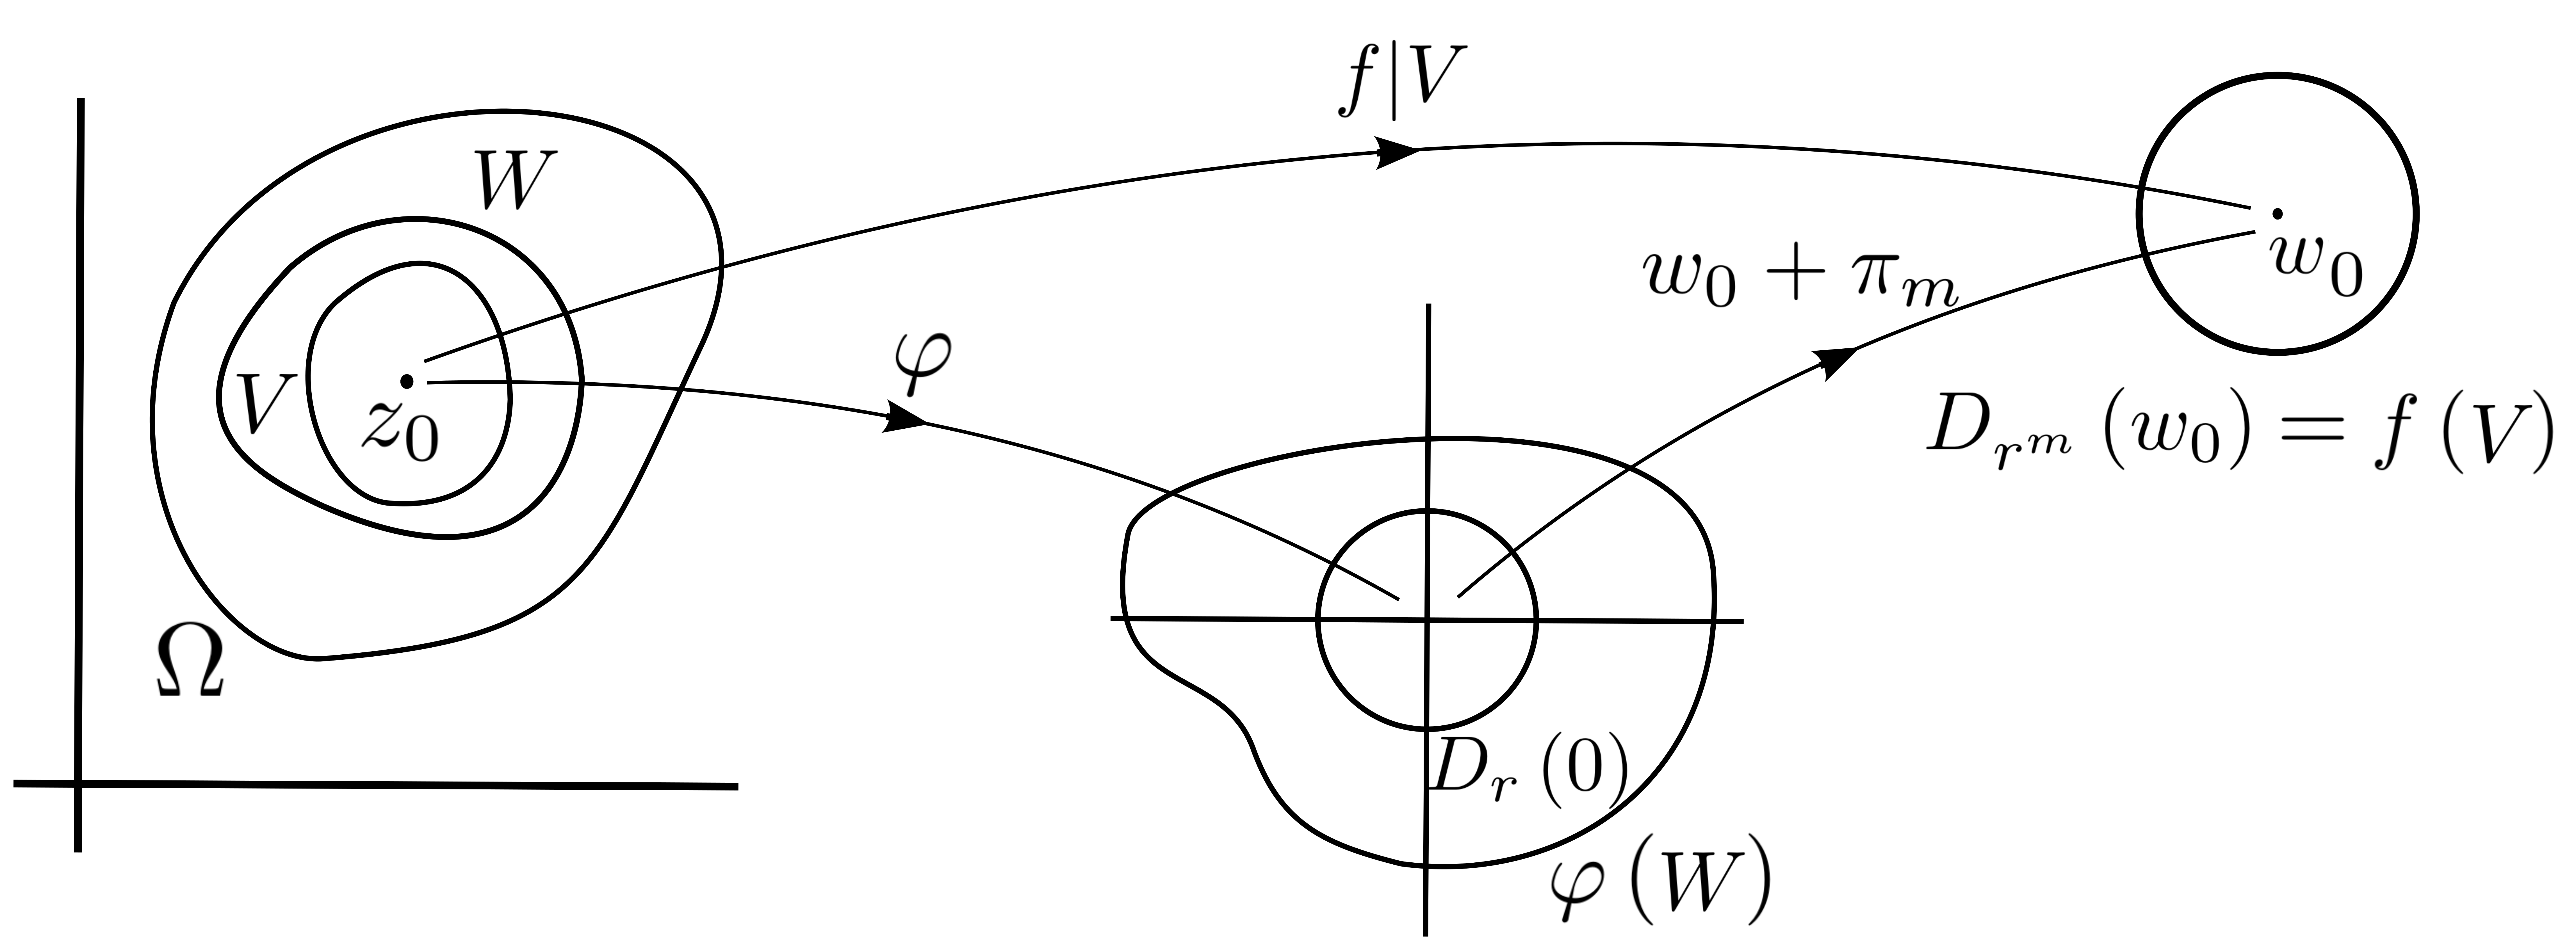
\includegraphics[width=0.8\textwidth]{20.png}
\end{center}


\textbf{Prova \ }Como a propriedade é de caracter local, não há
perda \ de generali-

dade em supor que $\Omega$ é uma vizinhança convexa de $z_{0}$
suficientemente pe-

quena de modo que $f(  z)  \neq w_{0}$ para cada $z\in
\Omega\backslash\left\{  z_{0}\right\}  $ (isto é possível pelo

princípio dos zeros isolados, Teor. 4.15). Então podemos escrever

\bigskip

$(  6.4.1)  $ \ \ \ \ \ \ \ \ \ \ \ $f(  z)
-w_{0}=(  z-z_{0})  ^{m}g(  z)  $ \ \ $\forall$
\ $z\in\Omega$

\bigskip

onde $g\in\mathcal{H}(  \Omega)  $ e $g(  z)  \neq0$
\ \ $\forall$ \ $z\in\Omega.$ Em consequência (ver cap. 1, Exemplo

3), temos $g^{\prime}/g\in\mathcal{H}(  \Omega)  $ e então pelo
teorema de Cauchy para um aberto

convexo (Teor. 5.7), existe $h\in\mathcal{H}(  \Omega)  $ tal que
$h^{\prime}=g^{\prime}/g.$ Consideremos a

função

\ \ \ \ \ \ \ \ \ \ \ \ \ \ \ \ \ \ \ \ \ \ \ \ \ \ \ \ $\psi:=g.\exp(
-h)  $ $.$

Como

\ \ \ \ \ \ \ \ \ \ \ \ \ \ \ \ \ $\psi^{\prime}=g^{\prime}\exp(
-h)  -gh^{\prime}\exp(  -h)  =(  g^{\prime}-gh^{\prime
})  \exp(  -h)  =0$

resulta que $\psi$ é constante em $\Omega,$ isto é

\ \ \ \ \ \ \ \ \ \ \ \ \ \ \ \ \ $\psi=g.\exp(  -h)  =k\in%
%TCIMACRO{\U{2102} }%
%BeginExpansion
\mathbb{C}
%EndExpansion
,$ \ em $\Omega$

\bigskip

e como $g\neq0$ em $\Omega,$ resulta $k\neq0$ portanto (ver Teor. 3.14 (j))
existe $\lambda\in%
%TCIMACRO{\U{2102} }%
%BeginExpansion
\mathbb{C}
%EndExpansion
$

tal que $\exp(  \lambda)  =k$ donde

\ \ \ \ \ \ \ \ \ \ \ \ \ \ \ \ $g=k\exp(  h)  =\exp(
h+\lambda)  ,$ em $\Omega$ $.$

Seja

\ \ \ \ \ \ \ \ \ \ \ \ \ \ \ \ \ \ \ \ \ \ \ \ \ \ \ \ \ \ \ \ \ $\ \ \ \ \ \ H:=h+\lambda
$

então\ 

$\ \ (  6.4.2)  $
\ \ \ \ \ \ \ $\ \ \ \ \ \ \ \ \ \ \ \ \ \ \ \ g=\exp(  H)  $

\bigskip

$(  6.4.3)  $
\ \ \ \ \ \ \ \ \ \ \ \ \ \ \ \ \ \ \ \ \ $\ \ \ \ H^{\prime}=g^{\prime}/g$

\bigskip

Definimos agora $\varphi:\Omega\rightarrow%
%TCIMACRO{\U{2102} }%
%BeginExpansion
\mathbb{C}
%EndExpansion
$ \ por

\ \ \ \ \ \ \ \ \ \ \ \ \ \ \ \ \ \ \ \ \ \ \ \ \ \ \ \ $\varphi(
z)  :=(  z-z_{0})  \exp(
%TCIMACRO{\QDABOVE{1pt}{H(  z)  }{m}}%
%BeginExpansion
\genfrac{}{}{1pt}{0}{H(  z)  }{m}%
%EndExpansion
)  $ \ \ $\forall$ \ $z\in\Omega$

\bigskip

e vamos mostrar que $\varphi$ satisfaz as condições do enunciado.

\bigskip

\textbf{Verificação de (a):}

\bigskip

$w_{0}\left[  \varphi(  z)  \right]  ^{m}=w_{0}+\left[  (
z-z_{0})  \exp(
%TCIMACRO{\QDABOVE{1pt}{H(  z)  }{m}}%
%BeginExpansion
\genfrac{}{}{1pt}{0}{H(  z)  }{m}%
%EndExpansion
)  \right]  ^{m}=w_{0}+(  z-z_{0})  ^{m}.\exp H(
z)  =$

\bigskip

$=w_{0}+(  z-z_{0})  ^{m}.g(  z)  =f(  z)  $
\ para cada $z\in\Omega,$ \ por $(  6.4.2)  $ e $(
6.4.1)  .$

\bigskip

\textbf{Verificação de (b):} \ É óbvio que $\varphi(
z_{0})  =0.$ Por outro lado, por $(  6.4.3)  $

resulta

\ \ \ \ \ \ \ \ \ \ \ \ \ \ \ \ \ \ \ $\varphi^{\prime}(  z)
=(  1+%
%TCIMACRO{\QDABOVE{1pt}{z-z_{0}}{m}}%
%BeginExpansion
\genfrac{}{}{1pt}{0}{z-z_{0}}{m}%
%EndExpansion
.%
%TCIMACRO{\QDABOVE{1pt}{g^{\prime}}{g}}%
%BeginExpansion
\genfrac{}{}{1pt}{0}{g^{\prime}}{g}%
%EndExpansion
)  \exp(
%TCIMACRO{\QDABOVE{1pt}{H(  z)  }{m}}%
%BeginExpansion
\genfrac{}{}{1pt}{0}{H(  z)  }{m}%
%EndExpansion
)  $ \ \ $\forall$ $\ z\in\Omega$

\bigskip

o que acarreta $\varphi^{\prime}(  z_{0})  =\exp(
%TCIMACRO{\QDABOVE{1pt}{H(  z_{0})  }{m}}%
%BeginExpansion
\genfrac{}{}{1pt}{0}{H(  z_{0})  }{m}%
%EndExpansion
)  \neq0.$ Pelo Teor. 6.2 \ resulta então

que existe uma vizinhança $W$ de $z_{0}$ em $\Omega$ tal que
$\varphi:W\rightarrow\varphi(  W)  $ é um iso-

morfismo analítico e que $\varphi^{\prime}(  \zeta)  \neq0$
\ $\forall$ \ $\zeta\in W$ \ (ver $(  6.4.2)  $). Como
$\varphi(  W)  $

é aberto e $0=\varphi(  z_{0})  \in\varphi(  W)  $,
existe $r>0$ tal que $D_{r}(  0)  \subset\varphi(  W)
,$ donde

$V:=\varphi^{-1}(  D_{r}(  0)  )  $ é uma
vizinhança aberta de $z_{0}$ contida em $W$ \ e visi-

velmente

\ \ \ \ \ \ \ \ \ \ \ \ \ \ \ \ \ \ \ \ \ \ \ \ \ \ \ \ $\varphi
|V:V\rightarrow D_{r}(  0)  $

é um isomorfismo analítico e $\varphi^{\prime}\neq0$ em $V$ pois
$\varphi^{\prime}\neq0$ em $V$ pois $\varphi^{\prime}\neq0$ em

$W\supset V.$

A última asserção do teorema agora é imediata pois se
$w_{1}\in D_{r^{m}}^{\ast}$ $(  w_{0})  ,$

então provar que a equação

\ \ \ \ \ \ \ \ \ \ \ \ \ \ \ \ \ \ \ \ \ \ \ \ \ \ \ \ \ \ \ \ \ \ \ \ \ \ $f(
z)  =w_{1}$

tem $m$ soluções (duas a duas diferentes) em $V,$ equivale a provar
que a

equação

\ \ \ \ \ \ \ \ \ \ \ \ \ \ \ \ \ \ \ \ $\pi_{m}\left[  \varphi(
z)  \right]  =\left[  \varphi(  z)  \right]^{m} = w_{1}%
-w_{0}$ \ \ \ \ \ $(  \neq0!)  $

\bigskip

tem $\ m$ soluções (duas a duas diferentes) em $V$ \ e sendo
$\varphi:V\rightarrow D_{r}(  0)  $ uma

aplicação bijetora, basta ver que a equação

$$\pi_{m}(  \zeta)  =\zeta^{m}=w_{1}-w_{0}$$

tem $m$ soluções (duas a duas diferentes) em $D_{r}(  0)
,$ o que é óbvio por ser

$w_{1}-w_{0}\neq0$ e pelo teorema de existência de raízes
$m$-ésima de um número

complexo não nulo. $\ \square$

\bigskip

\textbf{Observação 1 \ }Para $m>1$ a estrutura local de $f$ pode ser
descrita intui-

tivamente de forma bastante ilustrativa. Suponhamos para fixar idéias que

$m=3.$ Indicando com $w_{0}+\pi_{3}$ a aplicação $z\longmapsto
w_{0}+z^{3}$ e com as notações

do Teor. 6.4, a figura seguinte:

% IMAGEM 21

\begin{center}
  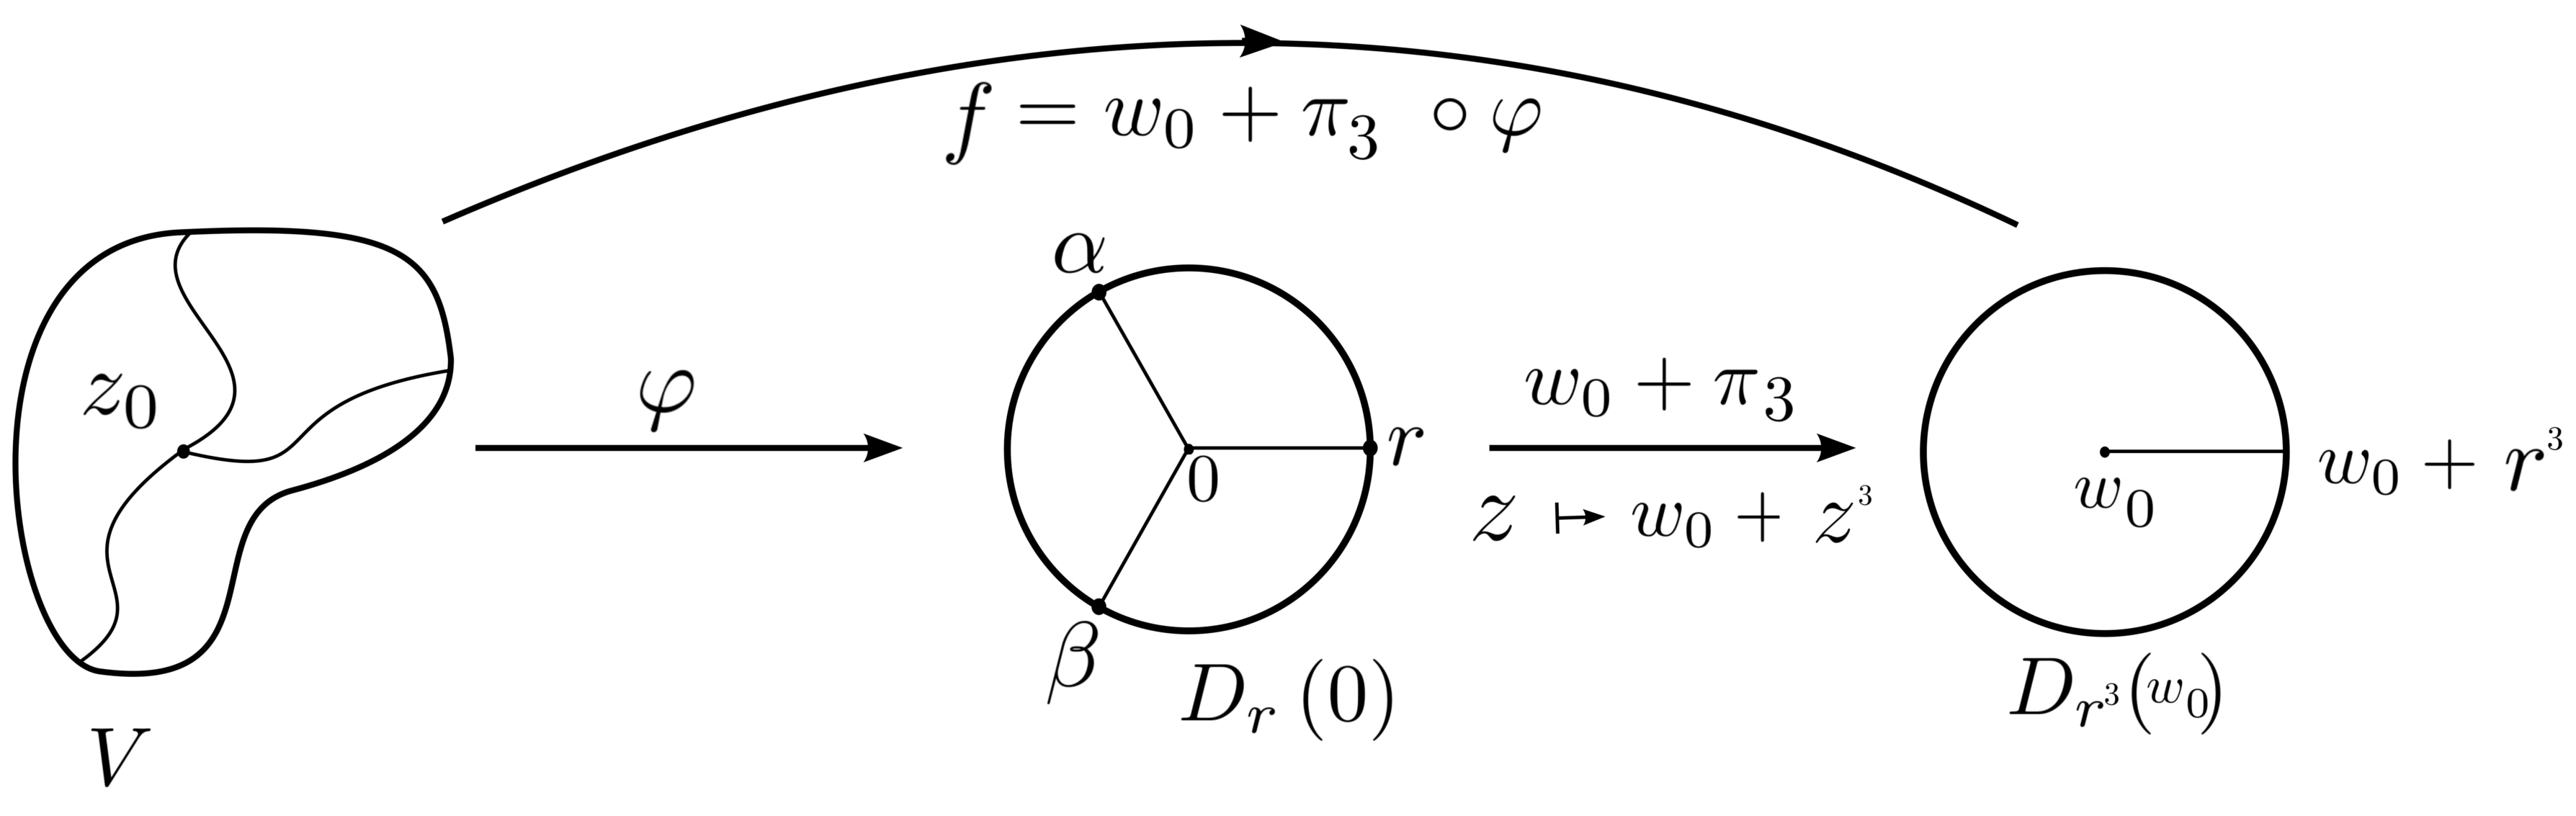
\includegraphics[width=0.8\textwidth]{21.png}
\end{center}

mostra a imagem inversa de $D_{r^{3}}(  w_{0})  $ e a imagem
inversa do raio $\left[  w_{0},w_{0}+r^{3}\right]  .$

Observar que $r,\alpha$ e $\beta$ são as três raízes cubicas de
$r^{3},$ isto é $\alpha=r_{\langle\frac{2\pi}{3}}$\ e

$\beta=r_{\langle\frac{4\pi}{3}}.$

\bigskip

\textbf{Observação 2} \ Se $\Omega$ não é conexo o Teor. 6.4
é falso pois se $A=D_{1}(  0)  ,$

$B=\left\{  z\in%
%TCIMACRO{\U{2102} }%
%BeginExpansion
\mathbb{C}
%EndExpansion
\text{ }|\text{ }\left\vert z\right\vert >2\right\}  ,$ $\Omega=A\cup B$ e
$f\in\mathcal{H}(  \Omega)  $ é definida por $f(
z)  =z^{3}$ \ \ 

$\forall$ \ $z\in A$ e $f|B=0,$ então $f$ não é constante e, por
exemplo, não podemos

nem falar da ordem do zero $z_{0}=3$ de $f=f-0=f-w$ .

\bigskip

\textbf{Corolário 6.5 \ }(teorema da aplicação aberta)
\ \textit{Se }$\Omega$ \textit{é um aberto conexo }

\textit{não vazio de }$%
%TCIMACRO{\U{2102} }%
%BeginExpansion
\mathbb{C}
%EndExpansion
,$ $f\in\mathcal{H}(  \Omega)  $ \textit{e }$f$ \textit{não
é constante, então }$f(  \Omega)  $ \textit{é aberto.}

\bigskip

\textbf{Prova \ }De fato, dado $w_{0}\in f(  \Omega)  $
arbitrário, seja $z_{0}\in\Omega$ tal que $f(  z_{0})  =w_{0}.$

Então, pelo Teor. 6.4 existe uma vizinhança $V$ de $z_{0\text{ }}$ em
$\Omega$ e existe $r>0$

tal que $f(  V)  =D_{r^{m}}(  w_{0})  ,$ onde $m$ é
a ordem do zero $z_{0}$ de $f-w_{0}.$ Como

$V\subset\Omega,$ resulta $f(  V)  =D_{r^{m}}(  w_{0})
\subset f(  \Omega)  ,$ o que mostra que $w_{0}$ é interior

a $f(  \Omega)  .$ \ $\square$

\bigskip

Se no Exemplo da Obs.2 acima modificamos a definição de $f$ em $B$

tomando por exemplo $f|B=1,$ com $f(  A)  =D_{1}(  0)  $
é claro que $f(  \Omega)  =$

$D_{1}(  0)  \cup\left\{  1\right\}  $ que não é aberto o
que mostra que o Corol. 6.5 é falso

se não supormos $\Omega$ conexo.

\bigskip

O resultado seguinte é a versão global do Teor. 6.2.

\bigskip

\textbf{Teorema 6.6 \ }( teorema da função inversa, versão global)
\ \textit{Seja }$\Omega$ \textit{um}

\textit{aberto conexo não vazio de }$%
%TCIMACRO{\U{2102} }%
%BeginExpansion
\mathbb{C}
%EndExpansion
,$ \textit{seja }$f\in\mathcal{H}(  \Omega)  $ \textit{e suponhamos
que }$f$ \textit{é}

\textit{injetora. Então }$f^{\prime}$ $(  z)  \neq
0$\textit{\ para cada }$z\in\Omega,$ $f$ \textit{é um isomorfismo
analí-}

\textit{tico de }$\Omega$ \textit{sobre }$f(  \Omega)  $ e

\ \ \ \ \ \ \ \ \ \ \ \ \ \ \ \ \ \ \ \ \ \ $f^{-1\prime}=%
%TCIMACRO{\QDABOVE{1pt}{1}{f^{\prime}\left[  f^{-1}(  w)  \right]
%}}%
%BeginExpansion
\genfrac{}{}{1pt}{0}{1}{f^{\prime}\left[  f^{-1}(  w)  \right]  }%
%EndExpansion
$ \ \ $\forall$ \ $w\in f(  \Omega)  $ $.$

\bigskip

\textbf{Prova \ }Suponhamos por absurdo que existe $z_{0}\in\Omega$ tal que
$f^{\prime}(  z_{0})  =0,$

então como $f$ não é constante e $\Omega$ é conexo e portanto
$f^{\prime}$ não pode ser

identicamente nula, $z_{0}$ é um zero isolado de $f^{\prime}$ e em
consequência (ver

exerc. 4.14) $z_{0}$ é um zero de $f-f(  z_{0})  $ de ordem
$m>1.$ PeloTeor.6.4

resulta então que localmente $f$ é uma função de tipo $(
m,1)  ;$ o que é ab-

surdo pois $m>1$ e $f$ é injetora, o que prova a primeira
asserção. Para

provar que $f$ é um isomorfismo analítico de $\Omega$ sobre $f(
\Omega)  $ e a asserção

relativa a derivada de $f^{-1},$ como $f^{\prime}(  z)  \neq0$ para
cada $z\in\Omega,$ basta aplicar

o Teor. 6.2. (c) em cada ponto de $\Omega$. \ $\square$

\bigskip

\textbf{Observação \ }A recíproca da primeira asserção do
Teor. 6.6 é falsa como

mostra o exemplo seguinte: $f(  z)  =e^{z}$ então $f^{\prime
}(  z)  =e^{z}\neq0$ para cada

$z\in%
%TCIMACRO{\U{2102} }%
%BeginExpansion
\mathbb{C}
%EndExpansion
,$ porém $f$ não é injetora. (pois é periódica, de
período $2\pi i$)

\bigskip

\textbf{Corolário 6.7} \ \textit{Sejam }$\Omega$\textit{\ um aberto conexo
não vazio de }$%
%TCIMACRO{\U{2102} }%
%BeginExpansion
\mathbb{C}
%EndExpansion
$\textit{\ e }$f\in\mathcal{H}(  \Omega)  ,$

\textit{então são equivalentes as condições seguintes}:

(i) \ $f$ \textit{é injetora,}

(ii) \ $f$\textit{\ é um isomorfismo analítico de }$\Omega$
\textit{sobre }$f(  \Omega)  .$ (em particular, vemos

que a condição (IA3) da Def. 6.3 é superflua)

\bigskip

\textbf{Prova \ }A implicação (ii) $\implies$ (i) é óbvia e a
implicação (i) $\implies$ (ii) está

contida no Teor. 6.6. \ $\square$

\bigskip

A seguir vamos expor algumas ideias básicas sobre o problema da inversão

global de funções analíticas (complexas) que, como veremos, é
mais compli-

cado que o seu análogo para funções reais. O Teor. 6.6 mostra que
o proble-

ma da inversão global de uma função $f\in\mathcal{H}(
\Omega)  ,$ $\Omega$ conexo, está resolvido se

$f$ é injetora. Se $\Omega$ é conexo e $f\in\mathcal{H}(
\Omega)  $ não é injetora, existem complexos

$w_{0}\in f(  \Omega)  $ tais que a equação $f(
z)  =w_{0}$ tem várias raízes distinta e se

poderia esperar que existissem várias funções $g_{1},g_{2},\ldots$
\ definidas em

$f(  \Omega)  $ tais que $f(  g_{1}(  w)  )
=w,$ $f(  g_{2}(  w)  )  =w,\ldots$ \ para todo $w\in
f(  \Omega)  .$

Temos com certa frequência uma situação deste tipo no caso real, por

exemplo, a função $f:x\in%
%TCIMACRO{\U{211d} }%
%BeginExpansion
\mathbb{R}
%EndExpansion
\longmapsto x^{2}\in%
%TCIMACRO{\U{211d} }%
%BeginExpansion
\mathbb{R}
%EndExpansion
$ tem como imagem $f(
%TCIMACRO{\U{211d} }%
%BeginExpansion
\mathbb{R}
%EndExpansion
)  =\left[  0,+\infty\right[  $

e existem duas funções contínuas $x\longmapsto\sqrt{x}$ e
$x\longmapsto-\sqrt{x}$ definidas em $f(
%TCIMACRO{\U{211d} }%
%BeginExpansion
\mathbb{R}
%EndExpansion
)  $

que são \ "inversas" \ de $f.$ Vamos ver que no caso complexo, a inversão

global não é tão simples. De modo mais preciso, \textit{se }%
$f\in\mathcal{H}(  \Omega)  $\textit{\ }($\Omega$\textit{\ conexo})

\textit{e }$f$\textit{\ não injetora, não existe em geral uma
função }$g\in\mathcal{C}(  f(  \Omega)  )
$\textit{\ tal que }

$f(  g(  w)  )  =w$\textit{\ \ para cada }$w\in f(
\Omega)  $ (este tipo de situação também pode

acontecer com funções reais de variável real)$,$\textit{\ em
consequência, não vai }

\textit{existir \ inversa analítica de }$f$\textit{\ em }$f(
\Omega)  .$O que vai ser possível é determinar

\underline{subconjuntos abertos maximais}$\ \ W_{\lambda}$ $(  \lambda
\in\Lambda)  $ de $f(  \Omega)  $ (em geral diferentes

de $f(  \Omega)  $) e funções $g_{\lambda}\in
\mathcal{H}(  W_{\lambda})  $ \ tais que \ \ \ \ \ \ \ \ \ \ \ \ 

\ \ \ \ \ \ \ \ \ \ \ \ \ \ \ \ \ \ \ \ $f(  g_{\lambda}(  w)
)  =w$ \ \ $\forall$ \ $w\in W_{\lambda}$ $.$

As vezes teremos a situação mais complicada seguinte: para cada
$\lambda\in\Lambda,$

existe uma família $(  g_{\lambda\alpha})  _{\alpha\in
A_{\lambda}}$ tal que $g_{\lambda\alpha}\in\mathcal{H}(  W_{\lambda
})  $ para cada $\alpha\in A_{\lambda}$ \ e

\ \ \ \ \ \ \ \ \ \ \ \ \ \ \ \ \ \ $f(  g_{\lambda\alpha}(
w)  )  =w$ \ \ $\forall$ \ $w\in W_{\lambda}$ \ e \ $\forall$
\ $\alpha\in A_{\lambda}$

\bigskip

Como ilustração e exemplo extremamente importante do que precede,

vamos definir as funções logaritmo complexo. Começamos com o seguinte

resultado do cálculo elementar. No que segue vamos a usar as notações

\bigskip

\ \ \ \ \ \ \ \ \ \ \ \ \ $L_{0}:=\left]  -\infty,0\right]  $ \ \ e
\ \ $D_{0}:=%
%TCIMACRO{\U{2102} }%
%BeginExpansion
\mathbb{C}
%EndExpansion
\backslash L_{0}=\left\{  z\in%
%TCIMACRO{\U{2102} }%
%BeginExpansion
\mathbb{C}
%EndExpansion
\text{ }|\text{ }z\neq-\left\vert z\right\vert \right\}  $

\bigskip

\textbf{Lema 6.8 }\textit{\ Para cada \ }$w=s+it\in D_{0}$\textit{\ \ existe
\ um único par }$(  r,\theta)  \in$

$%
%TCIMACRO{\U{211d} }%
%BeginExpansion
\mathbb{R}
%EndExpansion
_{+}^{\ast}\times\left]  -\pi,\pi\right[  $ \textit{tal que }$w=re^{i\theta}%
,$\textit{\ determinado pelas fórmulas}

\ \ \ \ \ \ \ \ \ \ \ \ \ \ \ \ \ \ \ \ \ 

\ \ \ \ \ \ \ \ \ \ \ \ \ \ $r=\sqrt{s^{2}+t^{2}}=\left\vert w\right\vert $
\ \ \ \ \ \ \textit{e \ \ \ \ \ \ }$\theta=2.Arctg%
%TCIMACRO{\QDABOVE{1pt}{t}{s+\left\vert w\right\vert }}%
%BeginExpansion
\genfrac{}{}{1pt}{0}{t}{s+\left\vert w\right\vert }%
%EndExpansion
$ $.$

\bigskip

\textbf{Prova \ }Suponhamos $\left\vert w\right\vert =1,$ então pelo Teor.
3.14 (i) existe $\tau\in%
%TCIMACRO{\U{211d} }%
%BeginExpansion
\mathbb{R}
%EndExpansion
$ tal

que $w=\exp(  i\tau)  =\cos\tau+i\operatorname{sen}\tau.$ Como
$\theta\longmapsto\exp(  i\theta)  $ \ (e portanto

$\theta\longmapsto\cos\theta$ \ e $\theta\longmapsto\operatorname{sen}\theta$)
tem período $2\pi,$ é claro que existe $\theta\in\left]  -\pi
,\pi\right]  $ \ 

tal que $\ w=\exp(  i\theta)  =\cos\theta+i\operatorname{sen}%
\theta$ e como $w\notin L_{0}$ é óbvio que $\theta\neq\pi,$

donde $\theta\in\left]  -\pi,\pi\right[  .$ É claro que este $\theta$
é único pois se $\theta_{1},\theta_{2}\in\left]  -\pi,\pi\right[  $ e

$w=\exp(  i\theta_{1})  =\exp(  i\theta_{2})  $
então $\exp\left[  i(  \theta_{1}-\theta_{2})  \right]  =1,$ o
que pelo Teor.

3.14 (g) implica $\theta_{1}-\theta_{2}=2k\pi$ com $k\in%
%TCIMACRO{\U{2124} }%
%BeginExpansion
\mathbb{Z}
%EndExpansion
$ e se fosse $k\neq0$ então

$\left\vert \theta_{1}-\theta_{2}\right\vert =2\left\vert k\right\vert \pi
\geq2\pi,$ o que é absurdo, portanto $k=0,$ isto é, $\theta_{1}%
=\theta_{2}.$

Consideremos agora o caso geral $w\in D_{0}$ então $w\neq0$ donde resulta

que podemos aplicar o que precede a $w/\left\vert w\right\vert :$ resulta que
\textit{existe um }

\textit{único }$\theta\in\left]  -\pi,\pi\right[  $ tal que

\ \ \ \ \ \ \ \ \ \ \ \ \ \ \ \ \ \ \ \ \ \ $%
%TCIMACRO{\QDABOVE{1pt}{w}{\left\vert w\right\vert }}%
%BeginExpansion
\genfrac{}{}{1pt}{0}{w}{\left\vert w\right\vert }%
%EndExpansion
=\exp(  i\theta)  =\cos\theta+i\operatorname{sen}\theta$

ou seja

\bigskip

$(  6.8.1)  $ \ \ \ \ \ \ \ \ \ \ \ \ \ \ \ $w=\left\vert
w\right\vert e^{i\theta}=\left\vert w\right\vert \cos\theta+i\left\vert
w\right\vert \operatorname{sen}\theta$ $.$

\bigskip

Ora, como $w=s+it,$ igualando partes real e imaginária, obtemos

$r:=\left\vert w\right\vert =\sqrt{s^{2}+t^{2}}$ \ e

\bigskip

$(  6.8.2)  $ \ \ \ \ \ \ \ \ \ \ \ \ \ \ \ $\cos\theta=sr^{-1}%
$\ \ \ \ \ \ ,\ \ \ \ \ \ $\operatorname{sen}\theta=tr^{-1}$.

\bigskip

Como $\theta\in\left]  -\pi,\pi\right[  $ é claro que $\theta/2\in\left]
-\pi/2,\pi/2\right[  $ e como neste intervalo a

função \ "tangente" (definida por $tg:=\operatorname{sen}/\cos$ \ fora
dos pontos de anulação

de \ "$\cos"$) é inversível, para determinar $\theta$ em
função dos dados $s,t$ e $w,$

será suficiente calcular $tg%
%TCIMACRO{\QDABOVE{1pt}{\theta}{2}}%
%BeginExpansion
\genfrac{}{}{1pt}{0}{\theta}{2}%
%EndExpansion
$ \ a partir de $(  6.8.2)  ,$ o que é imediato

$\bigskip$

$%
%TCIMACRO{\QDABOVE{1pt}{s}{r}}%
%BeginExpansion
\genfrac{}{}{1pt}{0}{s}{r}%
%EndExpansion
=\cos\theta=2\cos^{2}%
%TCIMACRO{\QDABOVE{1pt}{\theta}{2}}%
%BeginExpansion
\genfrac{}{}{1pt}{0}{\theta}{2}%
%EndExpansion
-1$ \ \ $\implies$ \ \ $2\cos^{2}%
%TCIMACRO{\QDABOVE{1pt}{\theta}{2}}%
%BeginExpansion
\genfrac{}{}{1pt}{0}{\theta}{2}%
%EndExpansion
=1+%
%TCIMACRO{\QDABOVE{1pt}{s}{r}}%
%BeginExpansion
\genfrac{}{}{1pt}{0}{s}{r}%
%EndExpansion
=%
%TCIMACRO{\QDABOVE{1pt}{r+s}{r}}%
%BeginExpansion
\genfrac{}{}{1pt}{0}{r+s}{r}%
%EndExpansion
$

\bigskip

$%
%TCIMACRO{\QDABOVE{1pt}{t}{r}}%
%BeginExpansion
\genfrac{}{}{1pt}{0}{t}{r}%
%EndExpansion
=\operatorname{sen}\theta=2\operatorname{sen}%
%TCIMACRO{\QDABOVE{1pt}{\theta}{2}}%
%BeginExpansion
\genfrac{}{}{1pt}{0}{\theta}{2}%
%EndExpansion
\cos%
%TCIMACRO{\QDABOVE{1pt}{\theta}{2}}%
%BeginExpansion
\genfrac{}{}{1pt}{0}{\theta}{2}%
%EndExpansion
$ \ , \ \ portanto

\bigskip

$\operatorname{tg}%
%TCIMACRO{\QDABOVE{1pt}{\theta}{2}}%
%BeginExpansion
\genfrac{}{}{1pt}{0}{\theta}{2}%
%EndExpansion
=%
%TCIMACRO{\QDABOVE{1pt}{2\operatorname{sen}\QDABOVE{1pt}{\theta}{2}%
%\cos\QDABOVE{1pt}{\theta}{2}}{2\cos^{2}\QDABOVE{1pt}{\theta}{2}}}%
%BeginExpansion
\genfrac{}{}{1pt}{0}{2\operatorname{sen}\genfrac{}{}{1pt}{0}{\theta}{2}%
\cos\genfrac{}{}{1pt}{0}{\theta}{2}}{2\cos^{2}\genfrac{}{}{1pt}{0}{\theta}{2}}%
%EndExpansion
=%
%TCIMACRO{\QDABOVE{1pt}{\QDABOVE{1pt}{t}{r}}{\QDABOVED{.}{.}{1pt}{r+s}{r}}}%
%BeginExpansion
\genfrac{}{}{1pt}{0}{\genfrac{}{}{1pt}{0}{t}{r}%
}{\genfrac{.}{.}{1pt}{0}{r+s}{r}}%
%EndExpansion
=%
%TCIMACRO{\QDABOVE{1pt}{t}{s+r}}%
%BeginExpansion
\genfrac{}{}{1pt}{0}{t}{s+r}%
%EndExpansion
=%
%TCIMACRO{\QDABOVE{1pt}{t}{s+\left\vert w\right\vert }}%
%BeginExpansion
\genfrac{}{}{1pt}{0}{t}{s+\left\vert w\right\vert }%
%EndExpansion
$ \ ,

\bigskip

donde $\theta=2\operatorname{Arctg}%
%TCIMACRO{\QDABOVE{1pt}{t}{s+\left\vert w\right\vert }}%
%BeginExpansion
\genfrac{}{}{1pt}{0}{t}{s+\left\vert w\right\vert }%
%EndExpansion
$ . Agora, com os valores de $\theta$ e $r$ calculados, o

resultado segue da primeira igualdade de $(  6.8.1)  .$ \ $\square$

\bigskip

Observe que (6.8.2) é rigoroso (isto é, sem uso da intuição geométrica)

pois por definição (ver Obs. $\left[  3\right]  $ \ que precede a
Prova \ (parcial) \ do

Teor. 3.14) tem-se $\cos\theta=\operatorname{Re}(  e^{i\theta})  $
e $\operatorname{sen}\theta:=$\textsc{I}m$(  e^{i\theta})  $
\ $\forall$ \ $\theta\in%
%TCIMACRO{\U{211d} }%
%BeginExpansion
\mathbb{R}
%EndExpansion
$ (o que aliás

foi usado na linha que precede a $(  6.8.1)  .$

\bigskip

Seja $w=s+it\in D_{0}$ com $s<0$ então $s=-\left\vert s\right\vert $ portanto

\bigskip

$%
%TCIMACRO{\QDABOVE{1pt}{t}{s+\left\vert w\right\vert }}%
%BeginExpansion
\genfrac{}{}{1pt}{0}{t}{s+\left\vert w\right\vert }%
%EndExpansion
=%
%TCIMACRO{\QDABOVE{1pt}{t}{\sqrt{s^{2}+t^{2}}-\left\vert s\right\vert }}%
%BeginExpansion
\genfrac{}{}{1pt}{0}{t}{\sqrt{s^{2}+t^{2}}-\left\vert s\right\vert }%
%EndExpansion
=%
%TCIMACRO{\QDABOVE{1pt}{t(  \sqrt{s^{2}+t^{2}}+\left\vert s\right\vert
%)  }{t^{2}}}%
%BeginExpansion
\genfrac{}{}{1pt}{0}{t(  \sqrt{s^{2}+t^{2}}+\left\vert s\right\vert
)  }{t^{2}}%
%EndExpansion
=%
%TCIMACRO{\QDABOVE{1pt}{\sqrt{s^{2}+t^{2}}+\left\vert s\right\vert }{t}}%
%BeginExpansion
\genfrac{}{}{1pt}{0}{\sqrt{s^{2}+t^{2}}+\left\vert s\right\vert }{t}%
%EndExpansion
$ $,$ \ o que

\bigskip

mostra que $\underset{t\rightarrow0^{\pm}}{\lim}%
%TCIMACRO{\QDABOVE{1pt}{t}{s+\left\vert w\right\vert }}%
%BeginExpansion
\genfrac{}{}{1pt}{0}{t}{s+\left\vert w\right\vert }%
%EndExpansion
=\pm\infty$ \ e em consequência

\bigskip

$(  (\ast))  $ \ \ \ \ \ \ \ \ \ \ \ \ $\underset{t\rightarrow
0^{\pm}}{\lim}\operatorname{Arctg}%
%TCIMACRO{\QDABOVE{1pt}{t}{s+\left\vert w\right\vert }}%
%BeginExpansion
\genfrac{}{}{1pt}{0}{t}{s+\left\vert w\right\vert }%
%EndExpansion
=\pm%
%TCIMACRO{\QDABOVED{.}{.}{1pt}{\pi}{2}}%
%BeginExpansion
\genfrac{.}{.}{1pt}{0}{\pi}{2}%
%EndExpansion
$

\bigskip

O Lema 6.8 (do qual utilizamos as notações) e as considerações acima

justificam a seguinte:

\bigskip

\textbf{Definição 6.9 \ }Dado $w=s+it\in D_{0}=%
%TCIMACRO{\U{2102} }%
%BeginExpansion
\mathbb{C}
%EndExpansion
\backslash L_{0}$ chama-se \textit{amplitude} (ou

\textit{\ argumento}) \ \textit{de} $w$ ao número real (pertencente a
$\left]  -\pi,\pi\right[  $)

\ \ \ \ \ \ \ \ \ \ \ \ \ \ \ \ \ \ \ \ \ \ \ \ \ 

$\ \ \ \ \ \ \ \ \ \ \ \ \ \ \ \ \ \ \ \ \ \ \ \ \ \ \ \ \ \ \ \ Am(
w)  :=2\operatorname{Arctg}%
%TCIMACRO{\QDABOVE{1pt}{t}{s+\left\vert w\right\vert }}%
%BeginExpansion
\genfrac{}{}{1pt}{0}{t}{s+\left\vert w\right\vert }%
%EndExpansion
$

\bigskip

Se $w\neq0$ e $w=s+it\in\left]  -\infty,0\right]  =L_{0}$ ( e portanto $t=0$ e
$s<0$) definimos

\bigskip

\ \ \ \ \ \ \ \ \ \ \ \ \ \ \ \ \ \ \ \ \ \ \ \ \ \ \ \ \ \ \ \ \ $Am(
w)  :=\pi$ \ $,$

\bigskip

isto é em virtude de $(  (  \ast)  )  ,$ $Am(
w)  :=\underset{\tau\rightarrow0^{+}}{\lim}Am(  s+i\tau)  . $

\bigskip

\textbf{Observação \ }(a) \ a prova do Lema 6.8 (e especialmente
$(  6.8.2)  $) mostram

que $\theta=Am(  w)  $ tem a interpretação geométrica
habitual, a saber, o \^{a}ngulo

orientado formado pelas semi-retas $\overrightarrow{Ow}$ e $%
%TCIMACRO{\U{211d} }%
%BeginExpansion
\mathbb{R}
%EndExpansion
_{+.}$

(b) \ $Am\in\mathcal{C}(  D_{0};\left]  -\pi,\pi\right[  )  .$ De
fato, a função

\bigskip

\ \ \ \ \ \ \ \ \ \ \ \ \ \ $\varphi:w=s+it\in D_{0}$ \ $\longmapsto$ \ $%
%TCIMACRO{\QDABOVE{1pt}{t}{s+\left\vert w\right\vert }}%
%BeginExpansion
\genfrac{}{}{1pt}{0}{t}{s+\left\vert w\right\vert }%
%EndExpansion
=%
%TCIMACRO{\QDABOVE{1pt}{t}{s+\sqrt{s^{2}+t^{2}}}}%
%BeginExpansion
\genfrac{}{}{1pt}{0}{t}{s+\sqrt{s^{2}+t^{2}}}%
%EndExpansion
\in%
%TCIMACRO{\U{211d} }%
%BeginExpansion
\mathbb{R}
%EndExpansion
%TCIMACRO{\QDABOVE{1pt}{{}}{{}}}%
%BeginExpansion
\genfrac{}{}{1pt}{0}{{}}{{}}%
%EndExpansion
$

\bigskip

é contínua pois $s+\sqrt{s^{2}+t^{2}}>0$ para cada \ $w=s+it\in
D_{0},$ o que mostra

que a função $Am,$ como composta de funções contínuas:

\bigskip

$\ \ \ \ Am:w=s+it\in D_{0}$ \ $\overset{\varphi}{\longmapsto}$ $%
%TCIMACRO{\QDABOVE{1pt}{t}{s+\left\vert w\right\vert }}%
%BeginExpansion
\genfrac{}{}{1pt}{0}{t}{s+\left\vert w\right\vert }%
%EndExpansion
$\ $\in%
%TCIMACRO{\U{211d} }%
%BeginExpansion
\mathbb{R}
%EndExpansion
$ \ $\overset{2\operatorname{Arctg}}{\longmapsto}$ \ $2\operatorname{Arctg}%
%TCIMACRO{\QDABOVE{1pt}{t}{s+\left\vert w\right\vert }}%
%BeginExpansion
\genfrac{}{}{1pt}{0}{t}{s+\left\vert w\right\vert }%
%EndExpansion
\in\left]  -\pi,\pi\right[  $

\bigskip

é contínua, o que prova (b).

\bigskip(c) \ Se $D_{0}\subsetneqq X\subset%
%TCIMACRO{\U{2102} }%
%BeginExpansion
\mathbb{C}
%EndExpansion
,$ \ e $\psi\in\mathcal{C}(  X)  $ então é falso
$\psi|D_{0}=Am$ \ ( ou em

linguagem menos precisa porém mais expressiva: \textit{a função}%
$\ Am$ \textit{não pode }

\textit{ser estendida} \textit{continuamente a nenhum ponto de}\ $L_{0}).$

Para provar esta afirmação fixemos $s_{0}\in X\cap\complement
D_{0}\subset L_{0}$ \ e suponhamos em

primeiro lugar que $s_{0}\neq0$ portanto $s_{0}<0.$ Será suficiente mostrar que

\ \ \ \ \ \ \ \ \ \ \ \ \ \ \ \ \ \ \ \ \ \ \ \ \ \ \ \ \ $\nexists
\underset{w\rightarrow s_{0}}{\lim}Am(  w)  $

e para isto, é suficiente provar que

\bigskip

$\left[  \ast\right]  $ \ \ \ \ \ \ \ \ \ \ \ \ \ \ \ \ \ \ \ $\underset
{t\rightarrow0^{+}}{\lim}Am(  s_{0}+it)  \neq\underset
{t\rightarrow0^{^{-}}}{\lim}Am(  s_{0}+it)  $ \ \ \ 

\bigskip

De fato, em vista da Def. 6.9, é claro que $(  (  \ast)
)  $ \ \ (três linhas acima da

Def. 6.9) \ \ \ pode ser escrita na forma

\bigskip

\ \ \ \ \ \ \ \ \ \ \ \ \ \ \ \ \ \ \ \ \ \ \ \ \ \ \ \ \ $\underset
{t\rightarrow0^{\pm}}{\lim}Am(  s_{0}+it)  = \pm\pi$

o que prova $\left[  \ast\right]  .$

\bigskip

Suponhamos agora que $\ s_{0}=0,$ então, para mostrar 

\bigskip

$\left[  \ast\ast\right]  $ \ \ \ \ \ \ \ \ \ \ \ \ \ \ $\nexists$
\ $\underset{w\rightarrow0}{\lim}Am(  w)  $

\bigskip

será suficiente verificar que, fixado $\alpha\in%
%TCIMACRO{\U{211d} }%
%BeginExpansion
\mathbb{R}
%EndExpansion
_{+}^{\ast}$ , quando $w\rightarrow0$ e $w$ percorrendo

a reta $y=\alpha x,$ o limite depende de $\alpha.$ Em termos mais precisos,
basta ver

que

\bigskip

$\left[  \ast\ast\ast\right]  $ \ \ \ \ \ \ \ $\underset{s\rightarrow0}{\lim
}Am(  s+i\alpha s)  $ é uma função não constante de
$\alpha.$ \ \ \ \ \ \ \ \ \ \ 

\bigskip

Ora, isto é claro pois para $s>0$ temos

\bigskip

$\varphi(  s+i\alpha s)  =%
%TCIMACRO{\QDABOVE{1pt}{\alpha s}{\sqrt{\alpha^{2}s^{2}+s^{2}}+s}}%
%BeginExpansion
\genfrac{}{}{1pt}{0}{\alpha s}{\sqrt{\alpha^{2}s^{2}+s^{2}}+s}%
%EndExpansion
=%
%TCIMACRO{\QDABOVE{1pt}{\alpha}{\sqrt{1+\alpha^{2}}+1}}%
%BeginExpansion
\genfrac{}{}{1pt}{0}{\alpha}{\sqrt{1+\alpha^{2}}+1}%
%EndExpansion
$

\bigskip

o que mostra que

\bigskip

\ \ \ \ \ \ \ \ \ \ \ \ \ \ \ \ \ \ \ \ \ \ $\underset{s\rightarrow0^{+}}%
{\lim}\varphi(  s+i\alpha s)  =%
%TCIMACRO{\QDABOVE{1pt}{\alpha}{1+\sqrt{1+\alpha^{2}}}}%
%BeginExpansion
\genfrac{}{}{1pt}{0}{\alpha}{1+\sqrt{1+\alpha^{2}}}%
%EndExpansion
$

\bigskip

que é uma função não constante de $\alpha$ (e, de passagem,
resulta que $\nexists$

$\underset{w\rightarrow0}{\lim}\varphi(  w)  $) donde segue que
$\left[  \ast\ast\ast\right]  $ \ pois:

\bigskip

$\underset{s\rightarrow0^{+}}{\lim}Am(  s+i\alpha s)
=\underset{s\rightarrow0^{+}}{\lim}2\operatorname{Arctg}(  \varphi(
s+i\alpha s)  )  =2\operatorname{Arctg}(  \underset
{s\rightarrow0^{+}}{\lim}\varphi(  s+i\alpha s)  )  =$

\bigskip

2$\operatorname{Arctg}(
%TCIMACRO{\QDABOVE{1pt}{\alpha}{1+\sqrt{1+\alpha^{2}}}}%
%BeginExpansion
\genfrac{}{}{1pt}{0}{\alpha}{1+\sqrt{1+\alpha^{2}}}%
%EndExpansion
)  $

\bigskip

que é visivelmente uma função não constante de $\alpha.$ Como
$\left[  \ast\ast\ast\right]  \implies\left[  \ast\ast\right]  ,$

a asserção (c) está completamente demonstrada.

\bigskip

Observar que

\bigskip

$(  (  \otimes)  )  $ \ \ \ \ \ \ \ \ \ $w=\left\vert
w\right\vert e^{iAm(  w)  }$ \ \ \ $\forall$ \ \ $w\in%
%TCIMACRO{\U{2102} }%
%BeginExpansion
\mathbb{C}
%EndExpansion
^{\ast}$

\bigskip

De fato, se $w\in D_{0}$, então $(  (  \otimes)  )  $
\ decorre do Lema 6.8 e se $w\in L_{0}\backslash\left\{  0\right\}  ,$

então $w$ é real negativo, isto é

\ \ \ \ \ \ \ \ \ \ \ \ \ \ \ \ \ \ \ \ $w=-\left\vert w\right\vert
=\left\vert w\right\vert e^{i\pi}=\left\vert w\right\vert e^{iAm(
w)  }$

pela Def. 6.9, o que prova $(  (  \otimes)  )  $ neste caso.

\bigskip

Lembremos que $f:%
%TCIMACRO{\U{2102} }%
%BeginExpansion
\mathbb{C}
%EndExpansion
\rightarrow%
%TCIMACRO{\U{2102} }%
%BeginExpansion
\mathbb{C}
%EndExpansion
$ é dita \underline{periódica de período} $\ p\in%
%TCIMACRO{\U{2102} }%
%BeginExpansion
\mathbb{C}
%EndExpansion
$ se:

(1%
%TCIMACRO{\U{ba}}%
%BeginExpansion
${{}^o}$%
%EndExpansion
) \ $p\neq0;$ \ \ (2%
%TCIMACRO{\U{ba}}%
%BeginExpansion
${{}^o}$%
%EndExpansion
) \ $f(  z+p)  =f(  z)  $ \ \ \ \ $\forall$ \ \ $z\in%
%TCIMACRO{\U{2102} }%
%BeginExpansion
\mathbb{C}
%EndExpansion
;$ \ \ (3%
%TCIMACRO{\U{ba}}%
%BeginExpansion
${{}^o}$%
%EndExpansion
) \ Se $q\in%
%TCIMACRO{\U{2102} }%
%BeginExpansion
\mathbb{C}
%EndExpansion
$ \ e

$f(  z+q)  =f(  z)  $ \ \ \ \ $\forall$ \ \ $z\in%
%TCIMACRO{\U{2102} }%
%BeginExpansion
\mathbb{C}
%EndExpansion
$ \ então $\left\vert p\right\vert \leq\left\vert q\right\vert .$

\bigskip

A função $\exp:z\in%
%TCIMACRO{\U{2102} }%
%BeginExpansion
\mathbb{C}
%EndExpansion
\longmapsto e^{z}\in%
%TCIMACRO{\U{2102} }%
%BeginExpansion
\mathbb{C}
%EndExpansion
$ é periódica de período $2\pi i.$ De fato, seja

$q\in%
%TCIMACRO{\U{2102} }%
%BeginExpansion
\mathbb{C}
%EndExpansion
^{\ast}$ tal que $\exp(  z+q)  =\exp z$ para cada $z\in%
%TCIMACRO{\U{2102} }%
%BeginExpansion
\mathbb{C}
%EndExpansion
,$ então pelo Teor. 3.14

(b), (c) resulta que $\exp(  q)  =1,$ portanto pelo Teor. 3.14 (g)
temos $%
%TCIMACRO{\QDABOVE{1pt}{q}{2\pi i}}%
%BeginExpansion
\genfrac{}{}{1pt}{0}{q}{2\pi i}%
%EndExpansion
\in%
%TCIMACRO{\U{2124} }%
%BeginExpansion
\mathbb{Z}
%EndExpansion
,$

logo

\ \ \ \ \ \ \ \ \ \ \ \ \ \ \ \ $\exp(  z+q)  =\exp(
z)  $ \ \ $\forall$ \ $z\in%
%TCIMACRO{\U{2102} }%
%BeginExpansion
\mathbb{C}
%EndExpansion
\iff%
%TCIMACRO{\QDABOVE{1pt}{q}{2\pi i}}%
%BeginExpansion
\genfrac{}{}{1pt}{0}{q}{2\pi i}%
%EndExpansion
\in%
%TCIMACRO{\U{2124} }%
%BeginExpansion
\mathbb{Z}
%EndExpansion
$

\bigskip

donde segue que $p=2\pi i$ é o período da função "$\exp".$
Resulta então que

"$\exp"$ não é injetora. A seguir vamos provar a existência de
\textit{subconjuntos }

\textit{abertos maximais} de

\ \ \ \ \ \ \ \ \ \ \ \ \ \ \ \ \ \ \ \ \ \ \ \ \ \ \ \ \ \ \ \ \ \ \ 

\ \ \ \ \ \ \ \ \ \ \ \ \ \ \ \ \ \ \ \ \ \ \ \ \ \ \ \ \ \ \ \ \ \ \ $\mathcal{I}%
$m$(  \exp)  =%
%TCIMACRO{\U{2102} }%
%BeginExpansion
\mathbb{C}
%EndExpansion
^{\ast}$ \ \ \ \ \ \ \ \ \ \ \ \ \ \ \ \ \ \ \ \ \ \ 

nos quais definiremos \ "determinações" (ou \ "ramos") da
função inversa de

"$\exp".$

\bigskip

\textbf{Lema 6.10} \ \textit{Seja }$w_{0}=s+it\in%
%TCIMACRO{\U{2102} }%
%BeginExpansion
\mathbb{C}
%EndExpansion
^{\ast}$ \ $(  s,t\in%
%TCIMACRO{\U{211d} }%
%BeginExpansion
\mathbb{R}
%EndExpansion
)  $ \textit{e seja }$z\in%
%TCIMACRO{\U{2102} }%
%BeginExpansion
\mathbb{C}
%EndExpansion
,$ \textit{então, as }

\textit{condições seguintes são equivalentes}:

(i) \ \ $e^{z}=w_{0}$

\bigskip(ii) \ $z=\ln\left\vert w_{0}\right\vert +i\left[  Am(
w_{0})  +2k\pi\right]  ,$ \ \textit{para algum }$k\in%
%TCIMACRO{\U{2124} }%
%BeginExpansion
\mathbb{Z}
%EndExpansion
.$

\bigskip

\textbf{Prova} \ (ii)$\implies$(i): \ Pela identidade $(  (
\otimes)  )  $ que precede a definição de função

periódica acima, temos

\bigskip

\ \ \ \ \ \ \ \ \ \ \ $e^{z}=e^{\ln\left\vert w_{0}\right\vert \text{ }%
}e^{i\left[  Am(  w_{0})  +2k\pi\right]  }=\left\vert
w_{0}\right\vert $ $e^{iAm(  w_{0})  }=w_{0}.$

\bigskip

(i)$\implies$(ii): \ Seja $z=x+iy$ \ $(  x,y\in%
%TCIMACRO{\U{211d} }%
%BeginExpansion
\mathbb{R}
%EndExpansion
)  $ tal que $e^{z}=w_{0}.$

Pela identidade $(  (  \otimes)  )  $ \ podemos escrever

\ \ \ \ \ \ \ \ \ \ \ \ \ \ \ \ \ 

\ \ \ \ \ \ \ \ \ \ \ \ \ \ \ $e^{z}=e^{x}$ $e^{iy}=w_{0}=\left\vert
w_{0}\right\vert e^{iAm(  w_{0})  }$

\bigskip

donde resulta

\bigskip

$(  6.10.1)  $ \ \ \ \ \ \ \ \ \ \ \ \ \ \ \ $e^{x}=\left\vert
w_{0}\right\vert $ \ \ e \ \ $e^{iy}=e^{iAm(  w_{0})  }$

\bigskip

A primeira das relações $(  6.10.1)  $ equivale a

\bigskip

$(  6.10.2)  $ \ \ \ \ \ \ \ \ \ \ \ \ \ \ \ \ \ $x=\ln\left\vert
w_{0}\right\vert $

\bigskip

Por outro lado, como $\ "\exp"$ tem período $2\pi i$ é claro que a função

$t\in%
%TCIMACRO{\U{211d} }%
%BeginExpansion
\mathbb{R}
%EndExpansion
\mapsto e^{it}\in%
%TCIMACRO{\U{2102} }%
%BeginExpansion
\mathbb{C}
%EndExpansion
$ tem período 2$\pi,$ em consequência, a segunda das relações

$(  6.10.1)  $ equivale a

\bigskip

$(  6.10.3)  $ \ \ \ \ \ \ $y=Am(  w_{0})  +2k\pi$ $,$
\ com \ $k\in%
%TCIMACRO{\U{2124} }%
%BeginExpansion
\mathbb{Z}
%EndExpansion
$

\bigskip

De $(  6.10.2)  $ e $(  6.10.3)  $ resulta (ii).
\ $\square$

\bigskip

\textbf{Lema 6.11 \ }\textit{Para cada }$k\in%
%TCIMACRO{\U{2124} }%
%BeginExpansion
\mathbb{Z}
%EndExpansion
$ \ \textit{seja}

\bigskip

\ \ \ \ \ \ \ \ \ \ \ \ \ \ \ \ \ \ $B_{k}:=\left\{  z\in%
%TCIMACRO{\U{2102} }%
%BeginExpansion
\mathbb{C}
%EndExpansion
|(  2k-1)  \pi<\text{Im}(  z)  <(  2k+1)
\pi\right\}  $

\textit{então:}

(1%
%TCIMACRO{\U{ba}}%
%BeginExpansion
${{}^o}$%
%EndExpansion
) \ \textit{A restrição }$\exp|B_{k}$ \ \textit{é injetora.}

(2%
%TCIMACRO{\U{ba}}%
%BeginExpansion
${{}^o}$%
%EndExpansion
) \ \textit{Se }$\Omega$ \textit{é um aberto de }$%
%TCIMACRO{\U{2102} }%
%BeginExpansion
\mathbb{C}
%EndExpansion
$\textit{\ tal que }$\Omega\supsetneqq B_{k}$ \textit{para algum }$k\in%
%TCIMACRO{\U{2124} }%
%BeginExpansion
\mathbb{Z}
%EndExpansion
,$ então

$\exp|\Omega$ \textit{não é injetora.}

(3%
%TCIMACRO{\U{ba}}%
%BeginExpansion
${{}^o}$%
%EndExpansion
) \ \textit{A imagem por \ "}$\exp"$ \textit{da reta }$y=b,$ \textit{onde
}$(  2k-1)  \pi<b<(  2k+1)  \pi$

\textit{para algum }$k\in%
%TCIMACRO{\U{2124} }%
%BeginExpansion
\mathbb{Z}
%EndExpansion
$ (portanto esta reta está contida em $B_{k}$) \textit{é a semireta}

\textit{aberta }$w=e^{x}\langle_{b}$ \ $(  x\in%
%TCIMACRO{\U{211d} }%
%BeginExpansion
\mathbb{R}
%EndExpansion
)  .$ \textit{Dados }$a\in%
%TCIMACRO{\U{211d} }%
%BeginExpansion
\mathbb{R}
%EndExpansion
$ \textit{e }$k\in%
%TCIMACRO{\U{2124} }%
%BeginExpansion
\mathbb{Z}
%EndExpansion
,$ \textit{a imagem do segmento }

\textit{aberto}

\ \ \ \ \ \ \ \ \ \ \ \ \ \ \ $S_{a,k}=\left\{  (  a,y)  |\text{
}(  2k-1)  \pi<y<(  2k+1)  \pi\right\}  $

\textit{pela função }$\ "\exp"$ \textit{é o círculo
}$\left\vert w\right\vert =e^{a}$ \ \textit{sem o ponto }$w=-e^{a}.$

(4%
%TCIMACRO{\U{ba}}%
%BeginExpansion
${{}^o}$%
%EndExpansion
) \ \textit{a imagem por }$\ "\exp"$ \textit{do aberto }$B_{k}$ \ $(
k\in%
%TCIMACRO{\U{2124} }%
%BeginExpansion
\mathbb{Z}
%EndExpansion
)  $ \ \textit{é o plano fendido}

\ $D_{0}=%
%TCIMACRO{\U{2102} }%
%BeginExpansion
\mathbb{C}
%EndExpansion
\backslash L_{0}=\left\{  z\in%
%TCIMACRO{\U{2102} }%
%BeginExpansion
\mathbb{C}
%EndExpansion
\text{ }|\text{ }z\neq-\left\vert z\right\vert \right\}  .$ \textit{Além
disso, se} $R_{k}:=\left\{  (  x,2(k+1) \pi)\text{ }|\text{ }x\in%
%TCIMACRO{\U{211d} }%
%BeginExpansion
\mathbb{R}
%EndExpansion
\right\} $
 
$\forall$ \ $ k$ \ $ \in \mathbb{Z}$ \ \textit{então} $\exp(  R_{k})  =L_{0}\backslash\left\{
0\right\}  $ \ $\forall$ \ $k\in \mathbb{Z}.$

% IMAGEM 23 (a 22 não foi usada)

\begin{center}
  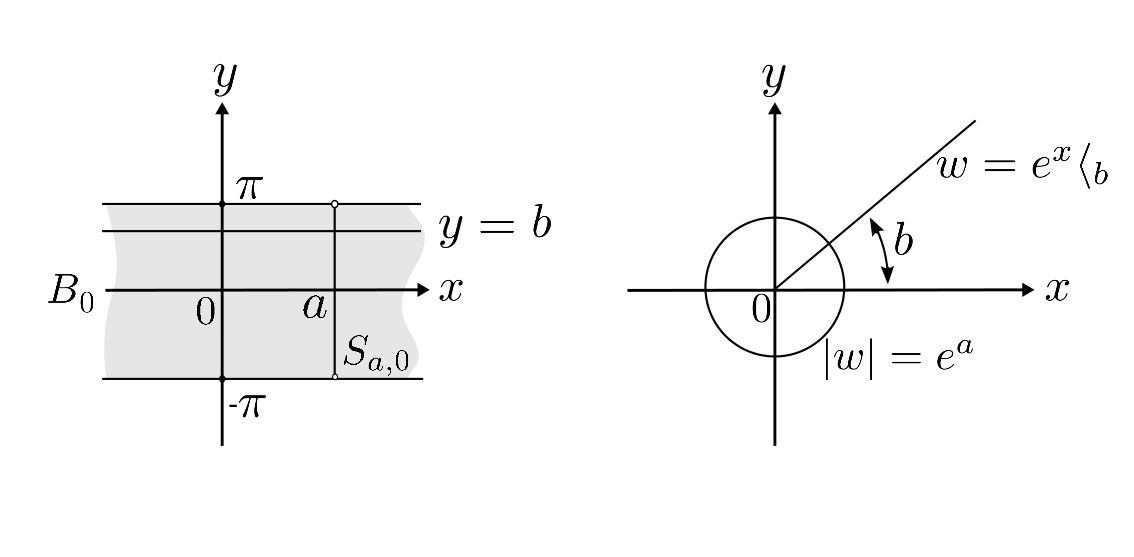
\includegraphics[width=0.8\textwidth]{23.png}
\end{center}

\textbf{Prova} \ (1%
%TCIMACRO{\U{ba}}%
%BeginExpansion
${{}^o}$%
%EndExpansion
) \ Fixados $k\in%
%TCIMACRO{\U{2124} }%
%BeginExpansion
\mathbb{Z}
%EndExpansion
$ arbitário, sejam $z_{1},z_{2}\in B_{k}$ tais \ que $e^{z_{1}}=e^{z_{2}}
$ \ 

e mostremos que $z_{1}=z_{2}.$ Seja $w=e^{z_{1}}=e^{z_{2}},$ então pelo
Lema 6.10

temos

\bigskip

\ \ \ \ \ \ \ \ \ \ \ \ \ \ \ \ \ \ \ \ \ \ \ \ $z_{1}=\ln\left\vert
w\right\vert +i\left[  Am(  w)  +2k_{1}\pi\right]  $ \ \ \ $,$
\ \ $k_{1}\in%
%TCIMACRO{\U{2124} }%
%BeginExpansion
\mathbb{Z}
%EndExpansion
$

\ \ \ \ \ \ \ \ \ \ \ \ \ \ \ \ \ \ \ \ \ \ \ \ $z_{2}=\ln\left\vert
w\right\vert +i\left[  Am(  w)  +2k_{2}\pi\right]  $ \ \ \ $,$
\ \ $k_{2}\in%
%TCIMACRO{\U{2124} }%
%BeginExpansion
\mathbb{Z}
%EndExpansion
$

donde:

\bigskip

$(  6.11.1)  $ \ \ \ \ \ \ \ \ \ $z_{1}-z_{2}=2i(  k_{1}%
-k_{2})  \pi$

\bigskip

Ora, como $z_{1},z_{2}\in B_{k}$ \ e ambos têm a mesma parte real $(
=\ln\left\vert w\right\vert )  ,$ resulta

$\left\vert z_{1}-z_{2}\right\vert <2\pi,$ o que por $(  6.11.1)  $
implica $k_{1}=k_{2},$ isto é $z_{1}=z_{2}.$

(2%
%TCIMACRO{\U{ba}}%
%BeginExpansion
${{}^o}$%
%EndExpansion
) \ Fixado $k\in%
%TCIMACRO{\U{2124} }%
%BeginExpansion
\mathbb{Z}
%EndExpansion
$ arbitrário, se $\Omega\supsetneqq B_{k}$ então existe $\zeta
\in\Omega$ tal que $\zeta\notin B_{k}$

portanto \ \ \ \ \ \ \ \ \ \ \ 

\ \ \ \ \ \ \ \ \ \ \ \ \ \ \ \ \ \ \ \ Im$(  \zeta)  \leq(
2k-1)  \pi$ \ \ ou \ \ Im$(  \zeta)  \geq(  2k+1)
\pi.$

Suponhamos, por exemplo, que Im$(  \zeta)  \geq(  2k+1)
\pi,$ então é claro que existe

$l\in%
%TCIMACRO{\U{2124} }%
%BeginExpansion
\mathbb{Z}
%EndExpansion
$ tal que

\ \ \ \ \ \ \ \ \ \ \ \ \ \ \ \ \ \ \ \ Im$(  \zeta)  -2l\pi
\in\left]  (  2k-1)  \pi,(  2k+1)  \pi\right[  $

donde, por definição de $B_{k}$ resulta:

\ \ \ \ \ \ \ \ \ \ \ \ \ \ \ \ \ \ \ \ $z:=\operatorname{Re}(
\zeta)  +i\left[  \text{Im}(  \zeta)  -2l\pi\right]  \in
B_{k}$

e então

\ \ \ \ \ \ \ \ \ \ $e^{z}=\exp\left\{  \operatorname{Re}(  \zeta)
+i\left[  \text{Im}(  \zeta)  -2l\pi\right]  \right\}  =\exp(
\zeta-2l\pi i)  =\exp(  \zeta)  =e^{\zeta},$

o que prova que $\exp|\Omega$ \ não é injetora pois $z\neq\zeta$

A asserção (3%
%TCIMACRO{\U{ba}}%
%BeginExpansion
${{}^o}$%
%EndExpansion
) é evidente e (4%
%TCIMACRO{\U{ba}}%
%BeginExpansion
${{}^o}$%
%EndExpansion
) decorre de (3%
%TCIMACRO{\U{ba}}%
%BeginExpansion
${{}^o}$%
%EndExpansion
). \ $\square$

\bigskip

Com a notação do Lema 6.11, seja

\ \ \ \ \ \ \ \ \ \ \ \ \ \ \ \ \ \ \ \ \ \ \ \ \ \ 

\ \ \ \ \ \ \ \ \ \ \ \ \ \ \ \ \ \ \ \ \ \ $f:=\exp|B_{0}$ $,$

\bigskip

então é claro que $\ f\in\mathcal{H}(  B_{0})  .$ Pelo Lema
6.11 (1%
%TCIMACRO{\U{ba}}%
%BeginExpansion
${{}^o}$%
%EndExpansion
) e (4%
%TCIMACRO{\U{ba}}%
%BeginExpansion
${{}^o}$%
%EndExpansion
) temos respec-

tivamente:

\bigskip

$\left[  1\right]  $ \ \ \ \ \ \ \ \ \ \ \ \ $f$ é injetora \ \ e
\ $f(  B_{0})  =D_{0}$

\bigskip

Consideremos a função

\ \ \ \ \ \ \ \ \ \ \ \ \ \ \ \ \ \ $g_{0}:w\in D_{0}\longmapsto\ln\left\vert
w\right\vert +iAm(  w)  \in%
%TCIMACRO{\U{2102} }%
%BeginExpansion
\mathbb{C}
%EndExpansion
$

\bigskip

Pelo Lema 6.8 e a Def. 6.9 temos $Am(  w)  \in\left]  -\pi
,\pi\right[  $ se $w\in D_{0}$ portanto,

pela definição de $B_{0}$ vem

\bigskip

\ \ \ \ \ \ \ \ \ \ \ $g_{0}(  w)  \in B_{0}=Dom(  f)
,$ \ \ para cada $w\in D_{0}$

\bigskip

em consequência está definido $f\left[  g_{0}(  w)
\right]  $ \ para cada $w\in D_{0}$ e o Lema 6.10

implica

\bigskip

$\left[  2\right]  $ \ \ \ \ \ \ \ \ \ \ \ \ \ $f\left[  g_{0}(
w)  \right]  =w$ \ \ \ \ \ \ \ \ \ \ $\forall$ \ \ $w\in D_{0}$

\bigskip

Por $\left[  1\right]  ,$ \ $f$ é uma bijeção de $B_{0}$ sobre
$D_{0},$ logo por $\left[  2\right]  $ e pelo exerc. 6.5

resulta que $g_{0}=f^{-1}.$ Pelo Teor. 6.6 temos que $f$ é um isomorfismos analítico

de $B_{0}$ sobre $D_{0},$ em consequência

\bigskip

$\left[  3\right]  $ \ \ \ \ \ \ \ \ \ \ $g_{0}=f^{-1}\in\mathcal{H}(
D_{0})  $

\bigskip

$\left[  4\right]  $ \ \ \ \ \ \ \ \ \ $g_{0}^{\prime}(  w)  =%
%TCIMACRO{\QDABOVE{1pt}{1}{f^{\prime}\left[  g_{o}(  w)  \right]
%}}%
%BeginExpansion
\genfrac{}{}{1pt}{0}{1}{f^{\prime}\left[  g_{o}(  w)  \right]  }%
%EndExpansion
$ \ \ \ \ \ \ \ \ \ \ $\forall$ \ \ $w\in D_{0}$

\bigskip

Como $f^{\prime}=f$ \ (ver Teor. 3.14 (e)), de $\left[  2\right]  $ e $\left[
4\right]  $ segue:

\bigskip

$\left[  5\right]  $ \ \ \ \ \ \ \ $g_{0}^{\prime}(  w)  =%
%TCIMACRO{\QDABOVE{1pt}{1}{w}}%
%BeginExpansion
\genfrac{}{}{1pt}{0}{1}{w}%
%EndExpansion
$ \ \ \ \ \ \ \ \ $\forall$ \ \ $w\in D_{0}.$

\bigskip

\textbf{Definição 6.12 \ }A função

\ \ \ \ \ \ \ \ \ \ \ \ \ \ \ \ \ \ \ \ \ \ \ \ \ \ \ $g_{0}:w\in
D_{0}\longmapsto\ln\left\vert w\right\vert +iAm(  w)  \in%
%TCIMACRO{\U{2102} }%
%BeginExpansion
\mathbb{C}
%EndExpansion
$

é chamada \textit{determinação} (ou \textit{ramo})
\textit{principal do logaritmo em}\ $D_{0}$ \ e \ é

indicado pela notação

\ \ \ \ \ \ \ \ \ \ \ \ \ \ \ \ \ \ \ \ \ \ \ \ \ \ \ \ \ \ \ \ \ \ \ \ \ $Log,$%


isto é \ \ \ \ $Log(  w)  =\ln\left\vert w\right\vert
+iAm(  w)  $ \ \ \ \ \ $\forall$ \ $w\in D_{0}.$

\bigskip

As fórmulas $\left[  2\right]  ,\left[  3\right]  $ e $\left[  5\right]  $
\ se escrevem:

\bigskip

$\left[  2^{\prime}\right]  $ \ \ \ \ \ \ \ \ \ $\exp(  Log(
w)  )  =w$ \ \ \ \ $\forall$ \ \ $w\in D_{o}$

\bigskip

$\left[  3^{\prime}\right]  $ \ \ \ \ \ \ \ \ $Log\in\mathcal{H}(
D_{0})  $

\bigskip

$\left[  5^{\prime}\right]  $ \ \ \ \ \ \ \ \ $Log^{\prime}(  w)  =%
%TCIMACRO{\QDABOVE{1pt}{1}{w}}%
%BeginExpansion
\genfrac{}{}{1pt}{0}{1}{w}%
%EndExpansion
$ \ \ \ \ \ $\forall$ \ \ $w\in D_{0}$

\bigskip

O disco aberto $D_{1}(  1)  $ é o maior disco aberto de centro
$1$ contido em $D_{0},$

logo pelo Corol. 4.11 resulta

\bigskip

\ \ \ \ \ \ \ \ \ \ $Log(  w)  =\underset{m\geq0}{%
%TCIMACRO{\dsum }%
%BeginExpansion
{\displaystyle\sum}
%EndExpansion
}%
%TCIMACRO{\QDABOVE{1pt}{Log^{(  m)  }(  1)  }{m!}}%
%BeginExpansion
\genfrac{}{}{1pt}{0}{Log^{(  m)  }(  1)  }{m!}%
%EndExpansion
(  w-1)  ^{m}$ \ \ \ \ $\forall$ \ \ $w\in D_{1}(  1)  $

\bigskip

A partir de $\left[  5^{\prime}\right]  $ resulta imediatamente por
indução que

\bigskip

\ \ \ \ \ \ \ \ \ \ \ \ \ \ \ \ \ $Log^{(  m)  }(  w)  =%
%TCIMACRO{\QDABOVE{1pt}{(  -1)  ^{m-1}\cdot(  m-1)
%!}{w^{m}}}%
%BeginExpansion
\genfrac{}{}{1pt}{0}{(  -1)  ^{m-1}\cdot(  m-1)
!}{w^{m}}%
%EndExpansion
$ \ \ \ \ $\forall$ \ \ $w\in D_{0},$ \ \ $\forall$ \ $\ m\in%
%TCIMACRO{\U{2115} }%
%BeginExpansion
\mathbb{N}
%EndExpansion
^{\ast}$

\bigskip

portanto fazendo $w-1=z$ no desenvolvimento de Taylor acima de $Log,$

obtemos

\ \ \ \ \ \ \ \ \ \ \ \ \ \ \ \ $Log(  1+z)  =\underset{m\geq1}{%
%TCIMACRO{\dsum }%
%BeginExpansion
{\displaystyle\sum}
%EndExpansion
}%
%TCIMACRO{\QDABOVE{1pt}{(  -1)  ^{m-1}}{m}}%
%BeginExpansion
\genfrac{}{}{1pt}{0}{(  -1)  ^{m-1}}{m}%
%EndExpansion
$ $z^{m}$ \ \ \ \ $z\in D_{1}(  0)  $

\bigskip

que é a forma habitual do desenvolvimento de Taylor da função
$Log.$

\bigskip

O próximo resultado fornece a informação básica para calcular
$"Log"$ de um

produto em $D_{0}$ de fatores em $D_{0}.$

\bigskip

\textbf{Proposição 6.13 \ }(1%
%TCIMACRO{\U{ba}}%
%BeginExpansion
${{}^o}$%
%EndExpansion
) $Log(  w^{-1})  =-Log(  w)  ,$ \ \textit{para cada
}$w\in D_{0}.$

(2%
%TCIMACRO{\U{ba}}%
%BeginExpansion
${{}^o}$%
%EndExpansion
) \ \textit{Se }$w_{1}\in D_{0}$ \textit{e }$w_{2}\in D_{0}$ \textit{são
tais que }$w_{1}w_{2}\in D_{0}$ \textit{então:}

\bigskip

$Log(  w_{1}w_{2})  =\left\{
\begin{array}
[c]{c}%
Log(  w_{1})  +Log(  w_{2})  ,\text{ \textit{se }}%
-\pi<Am(  w_{1})  +Am(  w_{2})  <\pi\\
Log(  w_{1})  +Log(  w_{2})  -2\pi i,\text{ \textit{se
}}Am(  w_{1})  +Am(  w_{2})  >\pi\text{ \ }\\
Log(  w_{1})  +Log(  w_{2})  +2\pi i,\text{ \textit{se
}}Am(  w_{1})  +Am(  w_{2})  <-\pi
\end{array}
\right.  $

\bigskip

(A hipótese $w_{1}w_{2}\in D_{0}$ exclui a possibilidade: $Am(
w_{1})  +Am(  w_{2})  =\pm\pi,$

ver Obs. logo após a prova da Prop. 6.13)

\bigskip

\textbf{Prova \ }(1%
%TCIMACRO{\U{ba}}%
%BeginExpansion
${{}^o}$%
%EndExpansion
) \ Como $w^{-1}=\overline{w}\left\vert w\right\vert ^{-2}$ resulta $Am(
w^{-1})  =Am(  \overline{w})  =-Am(  w)  $ \ 

(isto segue da Def. 6.9), donde $Log(  w^{-1})  =\ln\left\vert
w\right\vert ^{-1}-iAm(  w)  =-Log(  w)  .$

(2%
%TCIMACRO{\U{ba}}%
%BeginExpansion
${{}^o}$%
%EndExpansion
) \ Suponhamos verificadas as desigualdades:

\bigskip

$(  6.13.1)  $ \ \ \ \ \ \ \ \ \ \ \ $-\pi<Am(  w_{1})
+Am(  w_{2})  <\pi$

\bigskip

Pela identidade $(  (  \otimes)  )  $ \ que precede a
definição de função periódica

temos $w_{j}=\left\vert w_{j}\right\vert e^{iAm(  wj)  }$ \ \ se
$\ j=1,2,$ \ portanto multiplicando estas

identidades vem:

\bigskip

$(  6.13.2)  $ \ \ \ \ \ \ \ $w_{1}w_{2}=\left\vert w_{1}%
w_{2}\right\vert e^{i\left[  Am(  w_{1})  +Am(  w_{2})
\right]  }$

\bigskip

Por outro lado, aplicando de novo $((  \otimes)  )$\ a
$\ w_{1}w_{2}\in D_{0}\subset%
%TCIMACRO{\U{2102} }%
%BeginExpansion
\mathbb{C}
%EndExpansion
^{\ast}$ \ resulta

\bigskip

$(  6.13.3)  $ \ \ \ \ \ \ \ \ \ \ \ \ $w_{1}w_{2}=\left\vert
w_{1}w_{2}\right\vert e^{iAm(  w_{1}w_{2})  }$

\bigskip

De $(  6.13.1)  ,(  6.13.2)  $ e $(  6.13.3)
$ \ (pela unicidade no Lema 6.8) resulta

\bigskip

\ \ \ \ \ \ \ \ \ \ \ \ \ \ \ \ \ \ \ \ \ \ \ \ $Am(  w_{1}w_{2})
=Am(  w_{1})  +Am(  w_{2})  $

\bigskip

o que implica

$Log(  w_{1}w_{2})  =\ln\left\vert w_{1}w_{2}\right\vert +i\left[
Am(  w_{1})  +Am(  w_{2})  \right]  =\left[
\ln\left\vert w_{1}\right\vert +iAm(  w_{1})  \right]  +$

$\left[  \ln\left\vert w_{2}\right\vert +iAm(  w_{2})  \right]
=Log(  w_{1})  +Log(  w_{2})  .$

Suponhamos agora verificada a desigualdade $Am(  w_{1})  +Am(
w_{2})  >\pi,$ \ então

\bigskip

$(  6.13.4)  $ \ \ \ \ \ \ \ \ \ \ \ \ \ \ \ \ \ \ \ $\pi<Am(
w_{1})  +Am(  w_{2})  <2\pi$

\bigskip

Igualando os segundos membros de $(  6.13.2)  $ e $(
6.13.3)  $ e levando em consi-

deração de novo que $t\in%
%TCIMACRO{\U{211d} }%
%BeginExpansion
\mathbb{R}
%EndExpansion
\longmapsto e^{it}\in%
%TCIMACRO{\U{2102} }%
%BeginExpansion
\mathbb{C}
%EndExpansion
$ tem período $2\pi,$ resulta que existe

$k\in%
%TCIMACRO{\U{2124} }%
%BeginExpansion
\mathbb{Z}
%EndExpansion
$ tal que

\bigskip

$(  6.13.5)  $ \ \ \ \ \ \ \ $Am(  w_{1}w_{2})
+2k\pi=Am(  w_{1})  +Am(  w_{2})  $ $.$

\bigskip

Como $w_{1}w_{2}\in D_{0}$ e portanto $Am(  w_{1}w_{2})  \in\left]
-\pi,\pi\right[  ,$ de $(  6.13.4)  $ e $(  6.13.5)  $

resulta $k=1$ e então $(  6.13.5)  $ se escreve assim:

\ \ \ \ \ \ \ \ \ \ \ \ \ \ \ \ \ \ \ \ \ $Am(  w_{1}w_{2})
=Am(  w_{1})  +Am(  w_{2})  -2\pi$ $.$

Em consequência, a definição de $Log$ implica

$\ \ \ \ \ \ \ \ \ \ \ \ \ \ \ Log(  w_{1}w_{2})  =\ln\left\vert
w_{1}w_{2}\right\vert +i\left[  Am(  w_{1})  +Am(
w_{2})  -2\pi\right]  =$

$Log(  w_{1})  +Log(  w_{2})  -2\pi i$ $.$

\bigskip

O caso $Am(  w_{1})  +Am(  w_{2})  <-\pi$ \ é
inteiramente análogo. \ $\square$

\bigskip

\textbf{Observação \ }Vamos mostrar que a hipótese $w_{1}w_{2}\in
D_{0}$ implica $Am(  w_{1})  +$

$Am(  w_{2})  \neq\pm\pi.$ Igualando os segundos membros de
$(  6.13.2)  $ e $(  6.13.3)  $

obtemos $(  6.13.5)  $ para algum $k\in%
%TCIMACRO{\U{2124} }%
%BeginExpansion
\mathbb{Z}
%EndExpansion
$ \ e então, se fosse $\ Am(  w_{1})  +$

$Am(  w_{2})  =\pm\pi$ \ teríamos

\ \ \ \ \ \ \ \ \ \ \ \ \ \ \ \ \ $Am(  w_{1}w_{2})  =\pm\pi
-2k\pi=-(  2k\pm1)  \pi$

o que é absurdo pois por definição de $\ "Am"$ temos $Am(
w_{1}w_{2})  \in\left]  -\pi,\pi\right[  $ \ \ e

$-(  2k\pm1)  \pi\notin\left]  -\pi,\pi\right[  $ \ qualquer que
seja $k\in%
%TCIMACRO{\U{2124} }%
%BeginExpansion
\mathbb{Z}
%EndExpansion
.$

\bigskip

A seguir vamos determinar todas as determinações da função
logaritmo em

$D_{0}$ e, de forma mais geral, todas as determinações do logaritmo em abertos

conexos deduzidos de $D_{0}$ por rotação de centro na origem.

\bigskip

\textbf{Definição 6.14 \ }Seja $D$ um aberto conexo não vazio de $%
%TCIMACRO{\U{2102} }%
%BeginExpansion
\mathbb{C}
%EndExpansion
.$ Chama-se \textit{deter-}

\textit{minação} (\textit{ou ramo}) \textit{do logaritmo em} $D$ a
toda função $g\in\mathcal{C}(  D)  $ tal que

\ \ \ \ \ \ \ \ \ \ \ \ \ \ \ \ \ \ \ \ \ \ \ \ \ \ \ \ \ \ $\exp\left[
g(  w)  \right]  =w$ \ \ \ \ $\forall$ \ \ $w\in D.$

\bigskip

Observar que nas condições da Def. 6.14 temos $0\notin D$ em virtude
do Teor.

3.14 (c). O resultado seguinte determina todas as determinações do loga-

ritmo no aberto conexo $D_{0}=\left\{  z\in%
%TCIMACRO{\U{2102} }%
%BeginExpansion
\mathbb{C}
%EndExpansion
|\text{ }z\neq-\left\vert z\right\vert \right\}  .$

\bigskip

\textbf{Proposição \ 6.15 \ }\textit{Se }$g\in\mathcal{C}(
D_{0})  $ \textit{então as condições seguintes são
equi-}

\textit{valentes:}

(i) \ $\exp\left[  g(  w)  \right]  =w$ \textit{para cada }$w\in
D_{0}$ (i.e. $g$ é uma determinação do logarit-

mo em $D_{0})$

(ii) \ \textit{Existe }$k\in%
%TCIMACRO{\U{2124} }%
%BeginExpansion
\mathbb{Z}
%EndExpansion
$ \textit{tal que}

\ \ \ \ \ \ \ \ \ \ \ \ \ \ $g(  w)  =Log(  w)  +2k\pi
i,$ \ \textit{para cada }$w\in D_{0}.$

\bigskip

\textbf{Prova} \ (i)$\implies$(ii): \ Da definição de $Log$ resulta
\ (ver $\left[  2^{\prime}\right]  $):

\ \ \ \ \ \ \ \ \ \ \ \ \ \ \ \ \ \ \ \ $\exp\left[  Log(  w)
\right]  =w$ \ \ \ \ $\forall$ \ \ $w\in D_{0}$

então de (i) resulta

\ \ \ \ \ \ \ \ \ \ \ \ \ \ \ \ \ \ \ \ $\exp\left[  Log(  w)
\right]  =\exp\left[  g(  w)  \right]  $ \ \ \ \ $\forall$
\ \ $w\in D_{0}$

ou seja

\ \ \ \ \ \ \ \ \ \ \ \ \ \ \ \ \ \ \ $\exp\left[  g(  w)
-Log(  w)  \right]  =1$ \ \ \ \ $\forall$ \ \ $w\in D_{0}$

donde, pelo Teor. 3.14 (g) temos

\ \ \ \ \ \ \ \ \ \ \ \ \ \ \ \ \ $\varphi(  w)  :=%
%TCIMACRO{\QDABOVE{1pt}{1}{2\pi i}}%
%BeginExpansion
\genfrac{}{}{1pt}{0}{1}{2\pi i}%
%EndExpansion
\left[  g(  w)  -Log(  w)  \right]  \in%
%TCIMACRO{\U{2124} }%
%BeginExpansion
\mathbb{Z}
%EndExpansion
$ \ \ \ \ $\forall$ \ \ $w\in D_{0}$

Como $g\in\mathcal{C}(  D_{0})  ,$ resulta $\varphi\in
\mathcal{C}(  D_{0})  $ e como $D_{0}$ é conexo temos
$\varphi(  D_{0})  $ é

conexo e sendo $\varphi(  D_{0})  \subset%
%TCIMACRO{\U{2124} }%
%BeginExpansion
\mathbb{Z}
%EndExpansion
,$ resulta que $\varphi$ é constante, portanto existe

$k\in%
%TCIMACRO{\U{2124} }%
%BeginExpansion
\mathbb{Z}
%EndExpansion
$ tal que

\ \ \ \ \ \ \ \ \ \ \ \ \ \ \ \ $\varphi(  w)  =%
%TCIMACRO{\QDABOVE{1pt}{1}{2\pi i}}%
%BeginExpansion
\genfrac{}{}{1pt}{0}{1}{2\pi i}%
%EndExpansion
\left[  g(  w)  -Log(  w)  \right]  =k\in%
%TCIMACRO{\U{2124} }%
%BeginExpansion
\mathbb{Z}
%EndExpansion
$ \ \ \ \ $\forall$ \ \ $w\in D_{0},$

\bigskip

ou seja, existe $k\in%
%TCIMACRO{\U{2124} }%
%BeginExpansion
\mathbb{Z}
%EndExpansion
$ tal que

\ \ \ \ \ \ \ \ \ \ \ \ \ \ \ \ \ \ \ \ $g(  w)  =Log(
w)  +2k\pi i$ \ \ \ \ $\forall$ \ \ $w\in D_{0}$

\bigskip

(ii)$\implies$(i) \ Resulta imediatamente de $\left[  2^{\prime}\right]  $ e
do fato \ de "$\exp"$ \ ter

período $2\pi i:$

$\exp\left[  g(  w)  \right]  =\exp\left[  Log(  w)
+2k\pi i\right]  =\exp\left[  Log(  w)  \right]  =w,$ \ \ \ para \ cada

$w\in D_{0}.$ \ $\square$

\bigskip

Para cada $k\in%
%TCIMACRO{\U{2124} }%
%BeginExpansion
\mathbb{Z}
%EndExpansion
$ indicaremos no que segue pela notação $Log_{k}$ a função

$\ \ \ \ \ \ \ \ \ \ \ \ \ \ \ \ \ \ \ \ \ \ \ \ \ \ w\in D_{0}\longmapsto
Log(  w)  +2k\pi i\in%
%TCIMACRO{\U{2102} }%
%BeginExpansion
\mathbb{C}
%EndExpansion
$

(em particular vamos indicar $Log$ por $Log_{0}$). Como $Log_{k}$ é soma
da função

$Log\in\mathcal{H}(  D_{0})  $ com uma função constante
$(  w\longmapsto2k\pi i)  $ e portanto analítica,

é claro que

\ \ \ \ \ \ \ \ \ \ \ \ \ \ \ \ \ \ \ \ \ $Log_{k}\in\mathcal{H}(
D_{0})  $ \ \ \ \ $\forall$ \ \ $k\in%
%TCIMACRO{\U{2124} }%
%BeginExpansion
\mathbb{Z}
%EndExpansion
$

\bigskip

Pela Def. 6.14 e a Prop. 6.15 resulta que o conjunto enumerável ( de ele-

mentos de $\mathcal{H}(  D_{0})  $):

\ \ \ \ \ \ \ \ \ \ \ \ \ \ \ \ \ \ \ \ \ \ \ \ \ \ $\left\{  Log_{k\text{ }%
}|\text{ }k\in%
%TCIMACRO{\U{2124} }%
%BeginExpansion
\mathbb{Z}
%EndExpansion
\right\}  $

é o conjunto de todas as determinações do logaritmo em $D_{0}.$ Em
fim, é

claro agora (com notação do Lema 6.11) que

\ \ \ \ \ \ \ \ \ \ \ \ \ \ \ \ \ \ \ \ \ \ \ $Log_{k}=(  \exp|\text{
}B_{k})  ^{-1}$ \ \ \ \ $\forall$ \ \ $k\in%
%TCIMACRO{\U{2124} }%
%BeginExpansion
\mathbb{Z}
%EndExpansion
$

pois dado $w\in D_{0}$ arbitrário temos

\ \ \ \ \ \ \ \ \ \ \ \ \ \ \ \ \ \ \ \ \ \ $Log_{k}(  w)
=\ln\left\vert w\right\vert +i\left[  Am(  w)  +2k\pi\right]  $

e de $-\pi<Am(  w)  <\pi$ \ resulta

\ \ \ \ \ \ \ \ \ \ \ \ \ \ \ \ \ \ \ \ \ \ $(  2k-1)
\pi<Am(  w)  +2k\pi<(  2k+1)  \pi$

o que prova que

\ \ \ \ \ \ \ \ \ \ \ \ \ \ \ \ \ \ \ \ \ $Log_{k}(  w)  \in B_{k}$
\ \ \ \ $\forall$ \ \ \ $w\in D_{0}$ \ \ e \ \ $\forall$ \ \ $k\in%
%TCIMACRO{\U{2124} }%
%BeginExpansion
\mathbb{Z}
%EndExpansion
.$

\bigskip

\textbf{Proposição 6.16 \ }\textit{Sejam }$\alpha\in\left[
0,2\pi\right[  $ \textit{e }$D_{\alpha} \defeq e^{i\alpha}.D_{0}.$%
\textit{\ Então, para cada}

\textit{\ }$k\in%
%TCIMACRO{\U{2124} }%
%BeginExpansion
\mathbb{Z}
%EndExpansion
$ \textit{a função}

\ \ \ \ \ \ \ \ \ \ \ \ \ \ \ \ \ \ \ $Log_{k,\alpha}:w\in D_{\alpha
}\longmapsto i\alpha+Log_{k}(  e^{-i\alpha}.w)  \in%
%TCIMACRO{\U{2102} }%
%BeginExpansion
\mathbb{C}
%EndExpansion
$

\bigskip

\textit{é uma determinação do logaritmo em }$D_{\alpha}$ \ (ver
exerc. (6.8)).

\bigskip

\textbf{Prova \ }Como $Log_{k}$ é contínua em $D_{0}$ e a função $w\in D_{\alpha}\longmapsto
e^{-i\alpha}w\in D_{0}$

é contínua em $D_{\alpha},$ resulta que a função composta 

$w\in D_{\alpha}\longmapsto
Log_{k}(  e^{-i\alpha}.w)  \in%
%TCIMACRO{\U{2102} }%
%BeginExpansion
\mathbb{C}
%EndExpansion
$

é contínua em $D_{\alpha}$ e portanto:

\ \ \ \ \ \ \ \ \ \ \ \ \ \ \ \ \ \ \ \ \ \ $Log_{k,\alpha}\in\mathcal{C}%
(  D_{\alpha})  .$

Pela Def. 6.14, só resta verificar então que

\ \ \ \ \ \ \ \ \ \ \ \ \ \ \ \ \ \ \ \ $\exp\left[  Log_{k,\alpha}(
w)  \right]  =w$ \ \ \ \ $\forall$ \ \ $w\in D_{\alpha},$

\bigskip o que é trivial pois \ $\ \ \ \exp\left[  Log_{k,\alpha}(
w)  \right]  =\exp\left[  i\alpha+Log_{k}(  e^{-i\alpha}.w)
\right]  =$

$\exp(  i\alpha)  .\exp\left[  Log_{k}(  e^{-i\alpha}w)
\right]  =e^{i\alpha}(  e^{-i\alpha}w)  =w$ \ \ \ \ $\forall$
\ \ $w\in D_{\alpha}.$ \ $\square$

\bigskip

\begin{wrapfigure}[1]{r}{0.4\textwidth}
  \begin{center}
    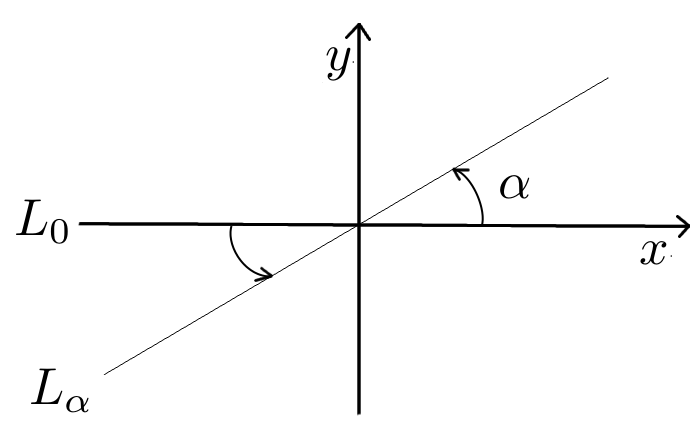
\includegraphics[width=0.4\textwidth]{fig4.png}
  \end{center}
\end{wrapfigure}

\textbf{Observação \ \ } Fixado %
$\alpha \in [0, 2\pi[$ como

na Proposição 6.16, sejam $D_{\alpha} = e^{-i\alpha}D_{0} =  $

$\mathbb{C}\backslash L_{\alpha}$, 
onde $L_{\alpha} \defeq e^{i\alpha}L_{0}$. Sejam $R_{-\alpha}:$

$w\in D_{\alpha} 
\longmapsto e^{-i\alpha}w \in D_{0}$ a transformação 

inversa de  $R_{\alpha}:w\in D_{0} 
\longmapsto e^{i\alpha}w \in D_{\alpha}$

($\therefore R_{\alpha}(D_{0}) = 
D_{\alpha} \text{ e } R_{-\alpha}(D_{\alpha}) = D_{0}$), 

$T_{i\alpha}:z 
\in \mathbb{C} \longmapsto \ z + i\alpha \in \mathbb{C}
$ e $B_{k,\alpha} \defeq $

$B_{k} + i\alpha =T_{i\alpha}(B_{k}) = $

$\{\zeta \in \mathbb{C} \textbar 
(2k - 1)\pi + \alpha < \zeta < (2k + 1)\pi + \alpha\}$. 

É claro então que $Log_{k, \alpha}$ é a seguinte com-

posta

\bigskip

$ Log_{k, \alpha}: w \in D_{\alpha} \overset{R_{-\alpha}}{\longmapsto} e^{-i\alpha}w \in D_{0} 
\overset{Log_{k}}{\longmapsto} Log_{k}(e^{-i\alpha}w) \in B_{k} \overset{T_{i\alpha}}{\longmapsto} $

$i\alpha + Log_{k}(e^{-i\alpha}w) 
\in B_{k} $

\bigskip

\begin{wrapfigure}{r}{0.4\textwidth}
  \begin{center}
    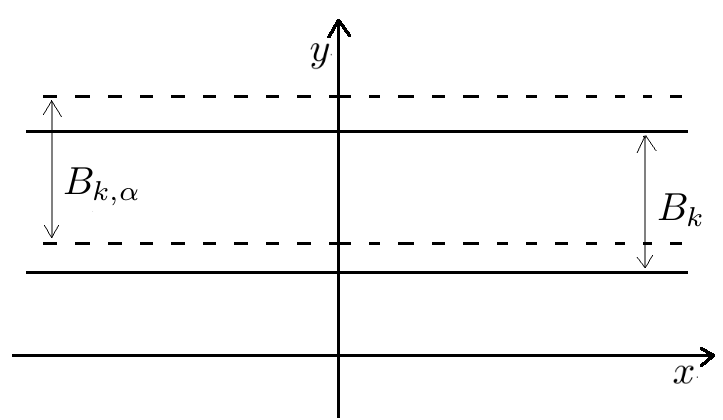
\includegraphics[width=0.4\textwidth]{fig5.png}
  \end{center}
\end{wrapfigure}


Como $R_{-\alpha}$ e $T_{i\alpha}$ são obviamente isomor-

fismos analíticos e $Log_{k}: D_{0} \longmapsto B_{k}$

 é um isomorfismo analítico de $D_{0}$ sobre 

$B_{k}$, é claro que $Log_{k,\alpha}:D_{\alpha} \longmapsto B_{k}$ é um

isomorfismo analítico de $D_{\alpha}$ sobre $B_{k,\alpha}$ 

cujo inverso é $\exp|B_{k}$ (em vista da 

relação ``$\exp[Log_{k,\alpha}(w)] = w, \forall w \in D_{\alpha}$'', 

ver a prova da Proposição 6.16), o que 

mostra que $\exp|B_{k,\alpha}$ é injetora e, mais 

ainda

$$ \exp|B_{k,\alpha}: B_{k,\alpha} \longmapsto D_{\alpha} $$

é um isomorfismo analítico de $B_{k,\alpha}$ sobre $D_{\alpha} $.

\bigskip

\textbf{Exemplo \ \ } Determinar a imagem e a inversa da função $Log_{2,\frac{\pi}{3}}$. Pela 

Observação anterior, é claro que $\mathcal{I}m(Log_{2,\frac{\pi}{3}}) = B_{2,\frac{\pi}{3}} = \{\zeta \in \mathbb{C} | 3\pi + \frac{\pi}{3}$

$ < \text{Im}(\zeta) < 5\pi + \frac{\pi}{3} \}$ e a inversa é $\exp|B_{2,\frac{\pi}{3}}: B_{2,\frac{\pi}{3}} \mapsto D_{\frac{\pi}{3}} 
( \defeq \mathbb{C} \backslash L_{\frac{\pi}{3}} )$.

\begin{center}
    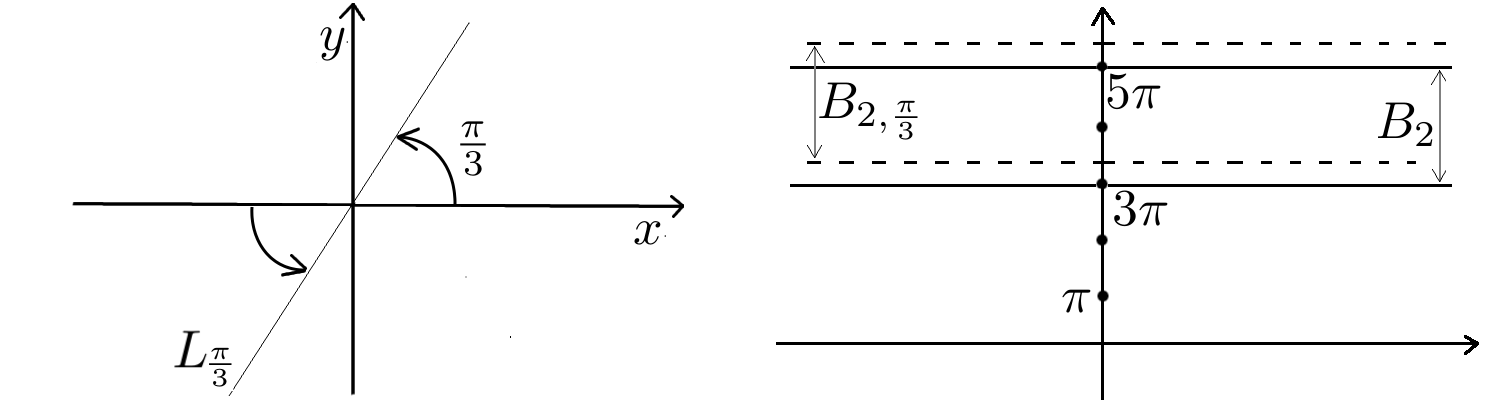
\includegraphics[width=\textwidth]{fig55.png}
  \end{center}

\bigskip

\textbf{Definição 6.17 \ \ }Seja $\lambda\in%
%TCIMACRO{\U{2102} }%
%BeginExpansion
\mathbb{C}
%EndExpansion
.$ A função

\ \ \ \ \ \ \ \ \ \ \ \ \ \ \ \ \ \ \ \ \ \ \ \ \ \ \ \ $z\in D_{0}\longmapsto
z^{\lambda}:=\exp\left[  \lambda Log(  z)  \right]  \in%
%TCIMACRO{\U{2102} }%
%BeginExpansion
\mathbb{C}
%EndExpansion
$

é chamada \textit{determinação}\ (ou \textit{ramo})
\textit{principal da potência} $\lambda$-\textit{ésima em} $D_{0}.$

\bigskip

É claro que $(  z\longmapsto z^{\lambda})  \in\mathcal{H}%
(  D_{0})  .$

\bigskip

\textbf{Exemplo \ }(1)\textbf{\ \ }Vamos calcular a determinação
principal de $i^{i}.$ Pela Def.

6.17 temos

$i^{i}=\exp\left[  iLog(  i)  \right]  =\exp\left[  i(
\ln\left\vert i\right\vert +iAm(  i)  )  \right]
=\exp(  -Am(  i)  )  =\exp(  -\pi/2)  =$

$e^{-\pi/2},$ isto é, \ $i^{i}=e^{-\pi/2}.$

\bigskip

(2) \ \underline{As determinações de} \ $\sqrt{z}$ \ $(
z\neq0)  $

A determinação principal de $\sqrt{z}$ é a função
$z\longmapsto\exp\left[
%TCIMACRO{\QDABOVE{1pt}{1}{2}}%
%BeginExpansion
\genfrac{}{}{1pt}{0}{1}{2}%
%EndExpansion
Log(  z)  \right]  ,$ \ vamos

calcular este valor.

$\exp\left[
%TCIMACRO{\QDABOVE{1pt}{1}{2}}%
%BeginExpansion
\genfrac{}{}{1pt}{0}{1}{2}%
%EndExpansion
Log(  z)  \right]  =\exp\left[
%TCIMACRO{\QDABOVE{1pt}{1}{2}}%
%BeginExpansion
\genfrac{}{}{1pt}{0}{1}{2}%
%EndExpansion
(  \ln\left\vert z\right\vert +iAm(  z)  )  \right]
=\exp(  \ln\sqrt{\left\vert z\right\vert })  .\exp(
%TCIMACRO{\QDABOVE{1pt}{i}{2}}%
%BeginExpansion
\genfrac{}{}{1pt}{0}{i}{2}%
%EndExpansion
Am(  z)  )  =$

$\bigskip$

$\sqrt{\left\vert z\right\vert }.1_{%
%TCIMACRO{\QDABOVED{\langle}{.}{1pt}{Am(  z)  }{2}}%
%BeginExpansion
\genfrac{\langle}{.}{1pt}{0}{Am(  z)  }{2}%
%EndExpansion
}=\sqrt{\left\vert z\right\vert }_{%
%TCIMACRO{\QDABOVED{\langle}{.}{1pt}{Am(  z)  }{2}}%
%BeginExpansion
\genfrac{\langle}{.}{1pt}{0}{Am(  z)  }{2}%
%EndExpansion
}$ \ portanto a detrminação principal da

função raíz quadrada é \ \ $z\in D_{0}$\ $\longmapsto
\sqrt{\left\vert z\right\vert }_{%
%TCIMACRO{\QDABOVED{\langle}{.}{1pt}{Am(  z)  }{2}}%
%BeginExpansion
\genfrac{\langle}{.}{1pt}{0}{Am(  z)  }{2}%
%EndExpansion
}$\ \ \ \ \ \ 

De modo análogo calculamos a determinação correspondente a
$Log_{1}$\ (em

vez de $Log=Log_{0}$\ \ que dá a principal):

$\bigskip$

$\exp\left[
%TCIMACRO{\QDABOVE{1pt}{1}{2}}%
%BeginExpansion
\genfrac{}{}{1pt}{0}{1}{2}%
%EndExpansion
Log_{1}(  z)  \right]  $\ $=\exp\left[
%TCIMACRO{\QDABOVE{1pt}{1}{2}}%
%BeginExpansion
\genfrac{}{}{1pt}{0}{1}{2}%
%EndExpansion
(  \ln\left\vert z\right\vert +i(  Am(  z)  +2\pi)
)  \right]  $\ $=\sqrt{\left\vert z\right\vert }.\exp(
%TCIMACRO{\QDABOVE{1pt}{i}{2}}%
%BeginExpansion
\genfrac{}{}{1pt}{0}{i}{2}%
%EndExpansion
(  Am(  z)$

$  +2\pi)  )  =\sqrt{\left\vert z\right\vert }.\exp(
%TCIMACRO{\QDABOVE{1pt}{i}{2}}%
%BeginExpansion
\genfrac{}{}{1pt}{0}{i}{2}%
%EndExpansion
Am(  z)  )  \exp(  i\pi)  =-\sqrt{\left\vert
z\right\vert }_{%
%TCIMACRO{\QDABOVED{\langle}{.}{1pt}{Am(  z)  }{2}}%
%BeginExpansion
\genfrac{\langle}{.}{1pt}{0}{Am(  z)  }{2}%
%EndExpansion
}$\ \ , logo esta determi-

nação é

\bigskip

$$z\in D_{0}\longmapsto
-\sqrt{\left\vert z\right\vert }_{%
%TCIMACRO{\QDABOVED{\langle}{.}{1pt}{Am(  z)  }{2}}%
%BeginExpansion
\genfrac{\langle}{.}{1pt}{0}{Am(  z)  }{2}%
%EndExpansion
}.$$

\bigskip

{É} imediato agora verificar que as duas determinações achadas
são as únicas

determinações da raíz quadrada \ em $D_{0}.$ De fato, o mesmo
tipo de cálculos

acima mostra que

\ \ \ \ \ \ 

\ \ \ \ \ \ \ \ \ \ $\exp\left[
%TCIMACRO{\QDABOVE{1pt}{1}{2}}%
%BeginExpansion
\genfrac{}{}{1pt}{0}{1}{2}%
%EndExpansion
Log_{k}(  z)  \right]  =(  -1)  ^{k}\sqrt{\left\vert
z\right\vert }_{%
%TCIMACRO{\QDABOVED{\langle}{.}{1pt}{Am(  z)  }{2}}%
%BeginExpansion
\genfrac{\langle}{.}{1pt}{0}{Am(  z)  }{2}%
%EndExpansion
}$ $\ ,$ \ isto é

\bigskip

$\ \ \ \ \ \ \ \exp\left[
%TCIMACRO{\QDABOVE{1pt}{1}{2}}%
%BeginExpansion
\genfrac{}{}{1pt}{0}{1}{2}%
%EndExpansion
Log_{k}(  z)  \right]  =\left\{
\begin{array}
[c]{c}%
\sqrt{\left\vert z\right\vert }_{%
%TCIMACRO{\QDABOVED{\langle}{.}{1pt}{Am(  z)  }{2}}%
%BeginExpansion
\genfrac{\langle}{.}{1pt}{0}{Am(  z)  }{2}%
%EndExpansion
}\text{ , \ se }k\text{ \ é par \ \ }\\
\text{\ \ \ }\\
-\sqrt{\left\vert z\right\vert }_{%
%TCIMACRO{\QDABOVED{\langle}{.}{1pt}{Am(  z)  }{2}}%
%BeginExpansion
\genfrac{\langle}{.}{1pt}{0}{Am(  z)  }{2}%
%EndExpansion
}\text{ \ , \ se }k\text{ é ímpar}%
\end{array}
\right.  $

\bigskip

Na lista de exercícios, no fim deste Capítulo,\ são enunciadas
as principais

propriedades das potências $\lambda$-ésimas.

\bigskip

Na Prop. A.2 (Apêndice do Capítulo 7) é dada uma
caracterização simples

dos abertos conexos nos quais existe uma determinação do logaritmo com-

plexo da qual segue trivialmente o Lema 6.18 abaixo. Entretanto, parece

útil resolver aqui mesmo, neste Capítulo 6, o problema da maximalidade

dos abertos $D_{\alpha}$ $(  \alpha\in\text{ }]0,2\pi\lbrack)  .$

\bigskip

\textbf{Lema 6.18 \ }\textit{Sejam }$a,b\in%
%TCIMACRO{\U{211d} }%
%BeginExpansion
\mathbb{R}
%EndExpansion
$ \textit{tais que }$0\leq a<b$ \ \textit{e}

\ \ \ \ \ \ \ \ \ \ \ \ \ \ \ \ \ \ \ \ $D:=\left\{  z\in%
%TCIMACRO{\U{2102} }%
%BeginExpansion
\mathbb{C}
%EndExpansion
\text{ }|\text{ }a<\left\vert z\right\vert <b\right\}  $

\textit{Então, não existe nenhuma determinação do logaritmo
complexo em }$D.$

\bigskip

\textbf{Prova \ }Suponha por absurdo que existe uma determinação do logaritmo

complexo em $D$, então (Def. 6.14) existe $g\in\mathcal{C}(
D)  $ tal que

\bigskip

$(  6.18.1)  $ \ \ \ \ \ \ \ \ \ \ \ \ \ \ \ \ $\exp\left[
g(  w)  \right]  =w$ \ \ \ \ $\forall$ \ \ $w\in D.$

\bigskip

Como $0\notin D,$ pelo Lema 6.10, a relação $(  6.18.1)  $
implica que $\forall$ \ $w\in D$

$\exists$ \ \ $k(  w)  \in%
%TCIMACRO{\U{2124} }%
%BeginExpansion
\mathbb{Z}
%EndExpansion
$ \ tal \ que $g(  w)  =\ln\left\vert w\right\vert +i\left[
Am(  w)  +2k(  w)  \pi\right]  ,$ logo \ podemos

escrever

\bigskip

$(  6.18.2)  $ \ \ \ \ $g(  w)  =\ln\left\vert
w\right\vert +i\left[  Am(  w)  +2k(  w)  \pi\right]  $
\ \ e \ \ $k(  w)  \in%
%TCIMACRO{\U{2124} }%
%BeginExpansion
\mathbb{Z}
%EndExpansion
,$ \ \ $\forall$ \ $w\in D.$

\bigskip

Da igualdade em $(  6.18.2)  $ resulta que a função

\bigskip

\ \ \ \ \ \ \ \ \ \ \ \ \ \ \ \ \ \ \ \ \ \ $\psi:w\in D\longmapsto Am(
w)  +2k(  w)  \pi\in%
%TCIMACRO{\U{211d} }%
%BeginExpansion
\mathbb{R}
%EndExpansion
$

\bigskip

é contínua [pois $\psi(  w)  =%
%TCIMACRO{\QDABOVE{1pt}{1}{i}}%
%BeginExpansion
\genfrac{}{}{1pt}{0}{1}{i}%
%EndExpansion
\left[  g(  w)  -\ln\left\vert w\right\vert \right]  $
\ \ $\forall$ \ \ $w\in D$ \ e \ $g$ \ e $\ln\left\vert \cdot\right\vert $ \ são

contínuas em $D$]. Em particular, $\psi$ é contínua em $D\cap
L_{0},$ vamos mostrar

que isto é absurdo. Fixemos $w_{0}\in D\cap L_{0}$ arbitrário, então

\bigskip

$\ \ \ \ \psi(  w_{0})  =\underset{t\rightarrow0^{\pm}}{\lim}%
\psi(  w_{0}+it)  =\underset{t\rightarrow0^{\pm}}{\lim}\left[
Am(  w_{0}+it)  +2\pi k(  w_{0}+it)  \right]  $

\bigskip

Como $\exists$ $\underset{t\rightarrow0^{\pm}}{\lim}Am(  w_{0}+it)
=\pm\pi\ $e\ $\exists$ \ $\underset{t\rightarrow0^{\pm}}{\lim}\left[
Am(  w_{0}+it)  +2\pi k(  w_{0}+it)  \right]  =$

$\psi(  w_{0})  ,$ concluimos que $\exists$ \ $\underset
{t\rightarrow0^{\pm}}{\lim}k(  w_{0}+it)  $ \ portanto a igualdade acima

pode ser escrita assim

\ \ \ \ \ \ \ \ \ \ \ \ \ \ \ \ \ \ \ \ \ \ \ 

$\ \ \ \ \ \ \ \ \ \ \ \ \ \ \ \ \ \ \ \ \ \psi(  w_{0})  =\pm
\pi+2\pi\underset{t\rightarrow0^{\pm}}{\lim}k(  w_{0}+it)  ,$ \ donde

\ \ \ \ \ \ \ \ \ \ \ \ \ \ \ \ \ \ \ \ \ 

\ \ \ \ \ \ \ \ \ \ \ \ \ \ \ \ \ \ \ \ \ \ $\underset{t\rightarrow0^{+}}%
{\lim}k(  w_{0}+it)  =%
%TCIMACRO{\QDABOVE{1pt}{1}{2\pi}}%
%BeginExpansion
\genfrac{}{}{1pt}{0}{1}{2\pi}%
%EndExpansion
(  \psi(  w_{0})  -\pi)  =:m\in%
%TCIMACRO{\U{2124} }%
%BeginExpansion
\mathbb{Z}
%EndExpansion
$

\bigskip

\ \ \ \ \ \ \ \ \ \ \ \ \ \ \ \ \ \ \ \ \ \ $\underset{t\rightarrow0^{-}}%
{\lim}k(  w_{0}+it)  =%
%TCIMACRO{\QDABOVE{1pt}{1}{2\pi}}%
%BeginExpansion
\genfrac{}{}{1pt}{0}{1}{2\pi}%
%EndExpansion
(  \psi(  w_{0})  +\pi)  =:n\in%
%TCIMACRO{\U{2124} }%
%BeginExpansion
\mathbb{Z}
%EndExpansion
$ $.$

\bigskip

Das definições de $m$ e $n$ resulta então

\ \ \ \ \ \ \ \ \ \ \ \ \ \ \ \ \ \ \ \ $\psi(  w_{0})  =\pi+2\pi
m=-\pi+2\pi n$ \ $\implies$ \ $2\pi=2\pi(  n-m)  $ \ logo

$n-m=1$ e portanto $n=m+1,$ donde resulta que $\exists$ $\ m\in%
%TCIMACRO{\U{2124} }%
%BeginExpansion
\mathbb{Z}
%EndExpansion
$ \ tal que

\bigskip

$(  6.18.3)  $ \ \ \ \ \ \ $\underset{t\rightarrow0+}{\lim}k(
w_{0}+it)  =m$ \ \ \ e \ \ \ $\underset{t\rightarrow0^{-}}{\lim}k(
w_{0}+it)  =m+1.$

\bigskip

Por outro lado no aberto \underline{conexo} \ $\omega:=D\cap\complement
L_{0},$ \ $Am$ é contínua (pois

$\omega\subset D_{0}$) \ e então, de $(  6.18.2)  ,$ resulta que

\ \ \ \ \ \ \ \ \ \ \ \ \ \ \ \ \ \ \ \ \ \ $w\in\omega\longmapsto k(
w)  \in%
%TCIMACRO{\U{2124} }%
%BeginExpansion
\mathbb{Z}
%EndExpansion
$

é contínua, logo constante $(  \omega\text{ é conexo}%
)  ,$ isto é, \ $\exists$ \ $\nu\in%
%TCIMACRO{\U{2124} }%
%BeginExpansion
\mathbb{Z}
%EndExpansion
$ \ tal que

\ \ \ \ \ \ \ \ \ \ \ \ \ \ \ \ \ \ \ $k(  w)  =\nu$
\ \ \ \ $\forall$ \ \ $w\in\omega,$

o que visivelmente está em contradição com $(  6.18.3)
.$ \ $\square$

% IMAGEM 24
\begin{center}
  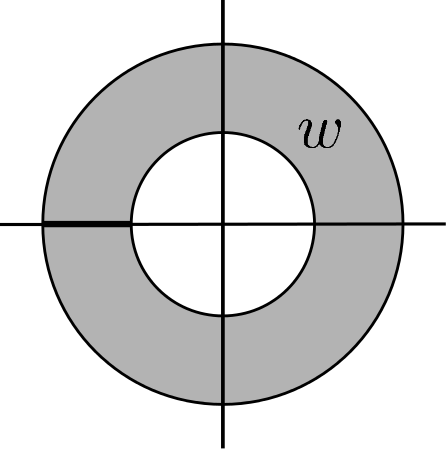
\includegraphics[width=0.27\textwidth]{24.png}
\end{center}

\textbf{Teorema 6.19 \ }\textit{Se }$\Omega$ \textit{é um aberto conexo de
}$%
%TCIMACRO{\U{2102} }%
%BeginExpansion
\mathbb{C}
%EndExpansion
$ \textit{tal que }$\Omega\supsetneqq D_{0}$ \textit{então}

\textit{não existe nenhuma determinação do logaritmo complexo em
}$\Omega.$

\bigskip

\textbf{Prova} \ Se $\Omega\supsetneqq D_{0}$ então existe $\zeta\in
\Omega\cap\complement D_{0}\subset L_{0},$ logo por definição

de aberto, existe $r>0$ tal que $D_{r}(  \zeta)  \subset\Omega,$
donde $\left]  \zeta-r,\zeta+r\right[  \subset\Omega.$ Como

$\zeta\in L_{0}$ temos $\zeta\leq0.$ Suponhamos que $\zeta<0$ \ então
é claro que podemos

supor $r<\left\vert \zeta\right\vert $ e, neste caso, $\Omega$ contem a "coroa"

\ \ \ \ \ \ \ \ \ \ \ \ \ \ \ \ \ \ \ \ \ \ \ \ \ \ \ \ \ \ $\left\{  z\in%
%TCIMACRO{\U{2102} }%
%BeginExpansion
\mathbb{C}
%EndExpansion
\text{ }|\text{ }\left\vert \zeta\right\vert -r<\left\vert z\right\vert
<\left\vert \zeta\right\vert +r\right\}  $

e a conclusão segue do Lema 6.18. Se $\zeta=0,$ então $\Omega$
contém a "coroa"

$\ \ \ \ \ \ \ \ \ \ \ \ \ \ \ \ \ \ \ \ \ \ \ \ \ \ \ \ \ \ \ \left\{  z\in%
%TCIMACRO{\U{2102} }%
%BeginExpansion
\mathbb{C}
%EndExpansion
\text{ }|\text{ }0<\left\vert z\right\vert <r\right\}  $

e de novo, a conclusão resulta do Lema 6.18. \ $\square$

\bigskip

\textbf{Corolário 6.20 \ }\textit{Se }$\alpha\in\lbrack0,2\pi\lbrack$
\textit{e }$\Omega$ \textit{é um aberto conexo de }$%
%TCIMACRO{\U{2102} }%
%BeginExpansion
\mathbb{C}
%EndExpansion
$ \textit{tal que}

$\Omega\supsetneqq D_{\alpha}(  :=e^{i\alpha}.D_{0})  ,$
\textit{então não existe nenhuma determinação do loga-}

\textit{ritmo complexo em }$\Omega.$

\bigskip

\textbf{Prova \ }De $\Omega\supsetneqq D_{\alpha}$ resulta $\Sigma
:=e^{-i\alpha}.\Omega\supsetneqq e^{-i\alpha}.D_{\alpha}=D_{0}.$ Se existisse

uma determinação g do logaritmo complexo em $\Omega$ então é
claro que a

função

\ \ \ \ \ \ \ \ \ \ \ \ \ \ $f:z\in\Sigma\longmapsto-i\alpha+g(
e^{i\alpha}.z)  \in%
%TCIMACRO{\U{2102} }%
%BeginExpansion
\mathbb{C}
%EndExpansion
$

seria uma determinação do logaritmo complexo em $\Sigma,$ o que é absurdo

em virtude do Teor. 6.19. \ $\square$

\bigskip

O Corol. 6.20 mostra que os conjuntos $D_{\alpha}(  \alpha\in\left[
0,2\pi\right[  )  $ são os subcon-

juntos abertos maximais de $\mathcal{I}$m$(  \exp)  =%
%TCIMACRO{\U{2102} }%
%BeginExpansion
\mathbb{C}
%EndExpansion
^{\ast}$ \ nos quais a função $"\exp"$ é

inversível, isto é, existem determinações do logaritmo complexo.

\bigskip

\bigskip

\ \ \ \ \ \ \ \ \ \ \ \ \ \ \ \ \ \ \ \ \ \ \ \ \ \ \ \ \ \ \ \ \ \ \ \ \ \ \ \ \ \ \ \textbf{Exercícios}%


\bigskip

\textbf{(6.1) \ }Sejam $\Omega$ um aberto conexo não vazio de $%
%TCIMACRO{\U{2102} }%
%BeginExpansion
\mathbb{C}
%EndExpansion
,$ $f\in\mathcal{H}(  \Omega)  ,$ \textsc{I}$=\left[  a,b\right]  $ \ um

intervalo compacto de $%
%TCIMACRO{\U{211d} }%
%BeginExpansion
\mathbb{R}
%EndExpansion
,$ $\ \varphi:$ \textsc{I}$\rightarrow%
%TCIMACRO{\U{2102} }%
%BeginExpansion
\mathbb{C}
%EndExpansion
$ \ e \ $\psi:$ \textsc{I}$\rightarrow%
%TCIMACRO{\U{2102} }%
%BeginExpansion
\mathbb{C}
%EndExpansion
$ \ duas funções \ Riemann-

integráveis e suponhamos que $\varphi(  t)  \notin f(
\Omega)  $ para cada $t\in$ \textsc{I.} Prove que a

função \ \ \ \ 

\ \ \ \ \ \ \ \ \ \ \ \ \ \ $F:z\in\Omega\longmapsto\underset{a}{%
%TCIMACRO{\dint }%
%BeginExpansion
{\displaystyle\int}
%EndExpansion
}^{^{b}\ }%
%TCIMACRO{\QDABOVE{1pt}{\psi(  t)  dt}{\varphi(  t)
%-f(  z)  }}%
%BeginExpansion
\genfrac{}{}{1pt}{0}{\psi(  t)  dt}{\varphi(  t)
-f(  z)  }%
%EndExpansion
$\ $\in%
%TCIMACRO{\U{2102} }%
%BeginExpansion
\mathbb{C}
%EndExpansion
$

\bigskip

é analítica em $\Omega.$ \ [\textbf{Sugestão: }\ Se $f=$cte.,
então $F=$cte.; se $f\neq$cte., então

$f(  \Omega)  $ é aberto e $F$ se escreve como composta das funções:

\bigskip

$\ \ \ \ \ \ \ z\in\Omega\overset{f}{\longmapsto}w=f(  z)  \in
f(  \Omega)  \longmapsto\underset{a}{%
%TCIMACRO{\dint }%
%BeginExpansion
{\displaystyle\int}
%EndExpansion
}^{b}%
%TCIMACRO{\QDABOVE{1pt}{\psi(  t)  dt}{\varphi(  t)
%-w}}%
%BeginExpansion
\genfrac{}{}{1pt}{0}{\psi(  t)  dt}{\varphi(  t)  -w}%
%EndExpansion
\in%
%TCIMACRO{\U{2102} }%
%BeginExpansion
\mathbb{C}
%EndExpansion
,$

\bigskip

a primeira das quais é analítica por hipótese e a segunda é
analítica pelo

Teor. 4.3]. Como aplicação, determine o maior aberto conexo $W$ de $%
%TCIMACRO{\U{2102} }%
%BeginExpansion
\mathbb{C}
%EndExpansion
$ no

qual é analítica a função

\ \ \ \ \ \ \ \ \ \ \ \ \ \ \ \ \ \ \ \ \ \ \ \ \ \ \ \ \ \ \ \ \ \ $F:z\in
W\longmapsto\underset{0}{%
%TCIMACRO{\dint }%
%BeginExpansion
{\displaystyle\int}
%EndExpansion
}^{1}%
%TCIMACRO{\QDABOVE{1pt}{\operatorname{sen}t\text{ }dt}{t^{2}-e^{z}}}%
%BeginExpansion
\genfrac{}{}{1pt}{0}{\operatorname{sen}t\text{ }dt}{t^{2}-e^{z}}%
%EndExpansion
\in%
%TCIMACRO{\U{2102} }%
%BeginExpansion
\mathbb{C}
%EndExpansion
$

\bigskip

\textbf{[Sugestão:} \ Como $t\in\left[  0,1\right]  \implies t^{2}%
\in\left[  0,1\right]  ,$ basta achar os $z\in%
%TCIMACRO{\U{2102} }%
%BeginExpansion
\mathbb{C}
%EndExpansion
$ tais que

$e^{z}\in\left[  0,1\right]  $ e eliminá-los. É imediato verificar que
$e^{z}\in\left[  0,1\right]  \iff z\in S_{k}$

onde $k\in%
%TCIMACRO{\U{2124} }%
%BeginExpansion
\mathbb{Z}
%EndExpansion
$ \ \ e $\ \ S_{k}=\left\{  z\in%
%TCIMACRO{\U{2102} }%
%BeginExpansion
\mathbb{C}
%EndExpansion
\text{ }|\text{ }\operatorname{Re}(  z)  \leq0\text{ e \textsc{I}%
m}(  z)  =2k\pi\right\}  ,$ \ \ portanto \ \ se $\ \ $

$\Omega=%
%TCIMACRO{\U{2102} }%
%BeginExpansion
\mathbb{C}
%EndExpansion
\backslash\underset{k\in%
%TCIMACRO{\U{2124} }%
%BeginExpansion
\mathbb{Z}
%EndExpansion
}{%
%TCIMACRO{\dbigcup }%
%BeginExpansion
{\displaystyle\bigcup}
%EndExpansion
}S_{k},$ \ \ então \ \ $F\in\mathcal{H}(  \Omega)  $\textbf{].}

\bigskip

\textbf{(6.2)} \ Determinar o maior disco aberto de centro na origem no qual

$f(  z)  =z^{2}+z$ seja injetora \ \ \textbf{[Sugestão:} A
condição $f(  \alpha)  =f(  \beta)  $ com

$\alpha\neq\beta$ implica $\alpha+\beta=-1$ logo $\alpha+\beta
=\operatorname{Re}(  \alpha)  +\operatorname{Re}(
\beta)  =-1$ o que mostra

que $f$ é injetora no disco $D_{1/2}(  0)  $ pois
$\operatorname{Re}(  \alpha)  >-1/2$ \ e \ $\operatorname{Re}%
(  \beta)  >-1/2$ \ 

portanto $\operatorname{Re}(  \alpha)  +\operatorname{Re}(
\beta)  >-1.$ Se $r>1/2$ então $f$ não é injetora em
$D_{r}(  0)  $

pois se o fosse, pelo Teor. 6.6 deveríamos ter $f^{\prime}(
z)  =2z+1\neq0$ para cada

$z\in D_{r}(  0)  ,$ o que é falso \ pois $f^{\prime}(
-1/2)  =0$ e $-1/2\in D_{r}(  0)  $\textbf{].}

\bigskip

\textbf{(6.3) \ }Determinar o maior disco aberto de centro na origem no qual

$f(  z)  =e^{z}$ seja injetora \textbf{[Sugestão:}\ Sabemos que
\ "$\exp"$ e uma bijeção da \ 

"banda"

\ \ \ \ \ \ \ \ \ \ \ \ \ \ \ $B_{k}=\left\{  z\in%
%TCIMACRO{\U{2102} }%
%BeginExpansion
\mathbb{C}
%EndExpansion
|\text{ }(  2k-1)  \pi<\text{\textsc{I}m}(  z)  <(
2k+1)  \pi\right\}  $ \ \ \ \ $(  k\in%
%TCIMACRO{\U{2124} }%
%BeginExpansion
\mathbb{Z}
%EndExpansion
)  $

sobre o plano fendido $D_{0}=\left\{  z\in%
%TCIMACRO{\U{2102} }%
%BeginExpansion
\mathbb{C}
%EndExpansion
\text{ }|\text{ }z\neq-\left\vert z\right\vert \right\}  .$ Em particular,
$\ "\exp"$

aplica $B_{0}$ sobre $D_{0},$ portanto o disco procurado é $D_{\pi}(
0)  $]

\bigskip

\textbf{(6.4) \ }Suponha que $\Omega$ é um aberto conexo, $\varphi
\in\mathcal{H}(  \Omega)  ,$ $\varphi^{\prime}$ não tem zeros

em $\Omega,$ $f\in\mathcal{H}(  \varphi(  \Omega)  )  ,
$ $g=f\circ\varphi,$ $z_{0}\in\Omega$ e $w_{0}=\varphi(  z_{0})  .$
Prove que se $w_{0}$ é

um zero de ordem $m$ de $f$, então $z_{0}$ é um zero de ordem $m$ de
$g.$ Como se

modifica esta situação se \ $z_{0}$ é um zero de ordem $k$ \ de
$\varphi^{\prime}$?

\bigskip

\textbf{(6.5) \ }Sejam $X$ e $Y$ dois conjuntos e $\beta:X\rightarrow Y$ uma
aplicação bijetora. Se

$\alpha:Y\rightarrow X$ tem a propriedade

\ \ \ \ \ \ \ \ \ \ \ \ \ \ \ \ \ \ \ \ \ \ \ \ \ \ \ \ \ $\beta\left[
\alpha(  y)  \right]  =y$ \ \ \ $\ \ \ \forall$ \ \ \ $y\in Y$

então $\alpha=\beta^{-1}.$

\bigskip

(6.6) (a) \ Sejam $k\in%
%TCIMACRO{\U{2124} }%
%BeginExpansion
\mathbb{Z}
%EndExpansion
$ e $X:=\{(w_{1},\ldots,w_{n})\in D_{0}^{n}$ \ $|$ $w:=\underset{j=1}%
{\overset{n}{%
%TCIMACRO{\dprod }%
%BeginExpansion
{\displaystyle\prod}
%EndExpansion
}}w_{j}\in D_{0}\}$.

Provar que: \ (I.) $X$ é um aberto de $%
%TCIMACRO{\U{2102} }%
%BeginExpansion
\mathbb{C}
%EndExpansion
^{n}$ ; \ (II.) Para cada componente

conexa $X_{0}$ de $X,$ existe $($ $k_{1},\ldots,k_{n}$ $)\in%
%TCIMACRO{\U{2124} }%
%BeginExpansion
\mathbb{Z}
%EndExpansion
^{n}$\ \ tal que

\ $\left[  \ast\right]  $\ \ \ \ \ \ \ \ \ \ \ \ \ \ \ $Log_{k}(
\overset{n}{\underset{j=1}{%
%TCIMACRO{\dprod }%
%BeginExpansion
{\displaystyle\prod}
%EndExpansion
}}w_{j})  =\underset{j=1}{\overset{n}{%
%TCIMACRO{\dsum }%
%BeginExpansion
{\displaystyle\sum}
%EndExpansion
}}Log_{k_{j}}(  w_{j})  $ \ \ \ $\forall$ \ \ $(  w_{1}%
,\ldots,w_{n})  \in X_{0}$ $.$

\bigskip

(b) \ Sejam $k\in%
%TCIMACRO{\U{2124} }%
%BeginExpansion
\mathbb{Z}
%EndExpansion
$ e $(  w_{1},\ldots,w_{n})  \in D_{0}^{n}$ \ tal que
$w:=\underset{j=1}{\overset{n}{%
%TCIMACRO{\dprod }%
%BeginExpansion
{\displaystyle\prod}
%EndExpansion
}}w_{j}\in D_{0}.$ Prove

que existe $(  k_{1},\ldots,k_{n})  \in%
%TCIMACRO{\U{2124} }%
%BeginExpansion
\mathbb{Z}
%EndExpansion
^{n}$ tal que

\ \ \ \ \ \ \ \ \ \ \ \ \ \ \ \ \ \ \ \ \ \ \ \ \ \ \ \ $Log_{k}(
\underset{j=1}{\overset{n}{%
%TCIMACRO{\dprod }%
%BeginExpansion
{\displaystyle\prod}
%EndExpansion
}}w_{j})  =\underset{j=1}{\overset{n}{%
%TCIMACRO{\dsum }%
%BeginExpansion
{\displaystyle\sum}
%EndExpansion
}}Log_{k_{j}}(  w_{j})  $ $.$

\bigskip

\textbf{Observação e sugestão:} É claro que o item (b) é
um caso particular do

item (a). O enunciado (b) afirma, em princípio, que a $n$-upla $(
k_{1},\ldots,k_{n})  $

$\in%
%TCIMACRO{\U{2124} }%
%BeginExpansion
\mathbb{Z}
%EndExpansion
^{n}$ \ depende da $\ n$-upla $(  w_{1},\ldots,w_{n})  \in X$
considerada. Já o enunciado

(a) mostra que a $n$-upla $(  k_{1,}\ldots,k_{n})  \in%
%TCIMACRO{\U{2124} }%
%BeginExpansion
\mathbb{Z}
%EndExpansion
^{n}$ depende da componente conexa

$X_{0}$ de $X,$ isto é, \ $(  k_{1},\ldots,k_{n})  \in%
%TCIMACRO{\U{2124} }%
%BeginExpansion
\mathbb{Z}
%EndExpansion
^{n}$ serve para cada $(  w_{1},\ldots,w_{n})  \in X_{0}.$

\textbf{[Sugestão para (a): \ }Fixe $(  w_{1}^{0},\ldots,w_{n}%
^{0})  \in X_{0}$ arbitrário portanto $w^{0}:=$

$\overset{n}{\underset{j=1}{%
%TCIMACRO{\dprod }%
%BeginExpansion
{\displaystyle\prod}
%EndExpansion
}}w_{j}^{0}\in D_{0}$ \ \ e

(1) \ \ $w^{0}=\left\vert w^{0}\right\vert \exp(  iAm(
w^{0})  )  $ \ e \ $w_{j}^{0}=\left\vert w_{j}^{0}\right\vert
\exp(  iAm(  w_{j}^{0})  )  $ \ $(  1\leq j\leq
n)  $

donde

\ \ \ \ \ \ \ \ \ \ \ \ \ \ \ \ \ \ \ \ \ \ \ $w^{0}=\left\vert w^{0}%
\right\vert \exp(  i\underset{j=1}{\overset{n}{%
%TCIMACRO{\dsum }%
%BeginExpansion
{\displaystyle\sum}
%EndExpansion
}}Am(  w_{j}^{0})  )  $

o que junto com a 1%
%TCIMACRO{\U{aa} }%
%BeginExpansion
${{}^a}$
%EndExpansion
identidade de (1) acarreta

\ \ \ \ \ \ \ \ \ \ \ \ \ \ \ \ \ \ \ \ \ \ $\exp\left[  i(  Am(
w^{0})  -\overset{n}{\underset{j=1}{%
%TCIMACRO{\dsum }%
%BeginExpansion
{\displaystyle\sum}
%EndExpansion
}}Am(  w_{j}^{0})  )  \right]  =1$

donde

(2) \ $\exists$ $\nu\in%
%TCIMACRO{\U{2124} }%
%BeginExpansion
\mathbb{Z}
%EndExpansion
$ tal que $Am(  w^{0})  -\underset{j=1}{\overset{n}{%
%TCIMACRO{\dsum }%
%BeginExpansion
{\displaystyle\sum}
%EndExpansion
}}Am(  w_{j}^{0})  =2\pi\nu$ . Como a função

(onde $w:=\overset{n}{\underset{j=1}{%
%TCIMACRO{\dprod }%
%BeginExpansion
{\displaystyle\prod}
%EndExpansion
}}w_{j}$)

\ \ \ \ \ \ \ \ \ \ \ \ \ \ \ \ \ \ \ \ \ \ \ $\Phi:(  w_{1},\ldots
,w_{n})  \in X_{0}\longmapsto Am(  w)  -\underset
{j=1}{\overset{n}{%
%TCIMACRO{\dsum }%
%BeginExpansion
{\displaystyle\sum}
%EndExpansion
}}Am(  w_{j})  \in%
%TCIMACRO{\U{211d} }%
%BeginExpansion
\mathbb{R}
%EndExpansion
$

é evidentemente contínua, o argumento usado para provar (2) mostra

que

$\Phi(  w_{1},\ldots,w_{n})  =2\pi\nu_{(  w_{1},\cdots
w_{n})  }$ $\forall$ $(w_{1},\ldots,w_{n})\in X_{0,}$ onde $\nu_{(
w_{1},\ldots w_{n})  }\in%
%TCIMACRO{\U{2124} }%
%BeginExpansion
\mathbb{Z}
%EndExpansion
.$ \ \ \ \ \ \ \ \ \ \ \ \ \ \ \ \ \ \ \ \ \ \ \ \ \ \ \ \ \ \ \ \ \ \ \ \ \ \ \ \ \ \ \ \ \ \ \ \ \ \ \ \ \ \ \ \ \ \ \ \ \ \ \ 

\bigskip

Como $\Phi$ é contínua, $X_{0}$ é conexo e \textsc{I}m$(
\Phi)  \subset\left\{  2\pi l\text{ }|\text{ }l\in%
%TCIMACRO{\U{2124} }%
%BeginExpansion
\mathbb{Z}
%EndExpansion
\right\}  ,$resulta que

$\Phi$ é constante logo da forma $2\pi\nu$ para algum $\nu\in%
%TCIMACRO{\U{2124} }%
%BeginExpansion
\mathbb{Z}
%EndExpansion
,$ isto é,

\bigskip

(3) \ $\exists$ \ $\nu\in%
%TCIMACRO{\U{2124} }%
%BeginExpansion
\mathbb{Z}
%EndExpansion
$ tal que $Am(  w)  -\overset{n}{\underset{j=1}{%
%TCIMACRO{\dsum }%
%BeginExpansion
{\displaystyle\sum}
%EndExpansion
}}Am(  w_{j})  =2\pi\nu$ $,$ \ $\forall$ \ \ $(  w_{1}%
,\ldots,w_{n})  \in X_{0}$

Considere a equação de $n$ incógnitas inteiras $x_{1},\ldots
,x_{n}:$

\bigskip

(4) \ \ \ \ \ \ \ \ \ \ \ \ \ \ \ \ \ \ \ \ \ \ \ \ \ \ \ \ \ $\underset
{j=1}{\overset{n}{%
%TCIMACRO{\dsum }%
%BeginExpansion
{\displaystyle\sum}
%EndExpansion
}}x_{j}=k+\nu$

É claro que (4) tem infinitas soluções em $%
%TCIMACRO{\U{2124} }%
%BeginExpansion
\mathbb{Z}
%EndExpansion
^{n},$ seja $(  k_{1},\ldots,k_{n})  \in%
%TCIMACRO{\U{2124} }%
%BeginExpansion
\mathbb{Z}
%EndExpansion
^{n}$

uma solução qualquer de (4) e mostre que vale $\left[  \ast\right]  $,
\ ver linha 4 do

exerc. (6.6).\textbf{]}

\bigskip

\textbf{(6.7) \ }Sejam\textbf{\ }$\alpha\in\lbrack0,2\pi\lbrack$ , $D_{\alpha
}:=e^{i\alpha}.D_{0}$ e, para cada $k\in%
%TCIMACRO{\U{2124} }%
%BeginExpansion
\mathbb{Z}
%EndExpansion
$ seja

\ \ \ \ \ \ \ \ \ \ \ \ \ \ \ \ \ \ \ \ \ \ \ \ 

$\ \ \ \ \ \ \ \ \ \ \ \ \ \ \ \ \ \ \ \ \ \ Log_{k,\alpha}:w\in D_{\alpha
}\longmapsto i\alpha+Log_{k}(  e^{-i\alpha}.w)  \in%
%TCIMACRO{\U{2102} }%
%BeginExpansion
\mathbb{C}
%EndExpansion
$

\bigskip

(onde $\left\{  Log_{k}\text{ }|\text{ }k\in%
%TCIMACRO{\U{2124} }%
%BeginExpansion
\mathbb{Z}
%EndExpansion
\right\}  $ denota o conjunto de todas as determinações do

logaritmo em $D_{0}$ $,Log_{0}=Log=$ det. principal do logaritmo em $D_{0}.$)

\textbf{(a) \ }Determine a imagem e a inversa de cada uma das funções seguintes:

\textbf{(I.) }\ $Log_{1,\pi/12}\in\mathcal{H}(  D_{\pi/2})  $
\ \ \ \ \ \ \ \ \ \ \ \textbf{\ (II.)} \ $Log_{-2,\pi/3}\in\mathcal{H}(
D_{\pi/3})  .$

\textbf{(b)}\ Fixado $\alpha\in\lbrack0,2\pi\lbrack$ prove que $\left\{
Log_{k,\alpha}\text{ }|\text{ }k\in%
%TCIMACRO{\U{2124} }%
%BeginExpansion
\mathbb{Z}
%EndExpansion
\right\}  $ é o conjunto de \textit{todas}

as determinações do logaritmo em $D_{\alpha}.$

\bigskip

\textbf{(6.8) \ }Prove as seguintes propriedades da determinação
principal da

potência em $D_{0}:$

\textbf{(a) }\ $z^{\lambda+\mu}=z^{\lambda}.z^{\mu}$ \ \ \ $\forall$ \ \ $z\in
D_{0},$ \ \ $\lambda,\mu\in%
%TCIMACRO{\U{2102} }%
%BeginExpansion
\mathbb{C}
%EndExpansion
$

\textbf{(b)} \ $(  z^{\lambda})  ^{\prime}=\lambda z^{\lambda-1}$
\ \ \ $\forall$ \ \ $z\in D_{0},$ \ \ \ $\lambda\in%
%TCIMACRO{\U{2102} }%
%BeginExpansion
\mathbb{C}
%EndExpansion
$

\textbf{(c)} \ Sejam $z_{1},z_{2}\in D_{0}$ tais que $z_{1}z_{2}\in D_{0}$ e
$-\pi<Am(  z_{1})  +Am(  z_{2})  <\pi.$

Mostre que $(  z_{1}z_{2})  ^{\lambda}=z_{1}^{\lambda}%
z_{2}^{\lambda}$ \ \ $\forall$ \ \ $\lambda\in%
%TCIMACRO{\U{2102} }%
%BeginExpansion
\mathbb{C}
%EndExpansion
.$

(d) \ As condições\textbf{\ \ }$\lambda,\mu\in%
%TCIMACRO{\U{2102} }%
%BeginExpansion
\mathbb{C}
%EndExpansion
$ \ e $z\in D_{0}$ \ tal que $z^{\lambda}\in D_{0},$ implicam

\ \ \ \ \ \ \ \ \ \ \ \ \ \ \ \ \ \ \ \ \ \ \ \ \ \ \ \ \ \ \ $(
z^{\lambda})  ^{\mu}=z^{\lambda\mu}$ $?$

\textbf{(e) \ }Calcule \ $\pi^{i},$ $i^{\pi},$ $(  1+i)  ^{1-i}$
\ e \ $(  -i)  ^{-i}$ \ (det. principais)

\textbf{Observação:} \ Se necessário, veja o livro de
Dieudonné \cite{D}, Calcul

Infinitesimal. \ \textbf{Sobre o item (d):} \ No livro citado acima
(pg 258) se pede

para provar a seguinte afirmação

\bigskip$(  (  \ast)  )  $ \ \ \ $\lambda,\mu\in%
%TCIMACRO{\U{2102} }%
%BeginExpansion
\mathbb{C}
%EndExpansion
,$ \ $z\in D_{0\text{ \ }}$ e \ $z^{\lambda}\in D_{0}\implies(
z^{\lambda})  ^{\mu}=z^{\lambda\mu}$

\textbf{(I.) \ }Prove com um contra-exemplo que $(  (  \ast)
)  $ é falsa \textbf{[Sugestão: }$z=e,$

$\lambda=2\pi i$ \ e \ $\mu=i.\mathbf{];}$

\textbf{(II.) \ }Suponha agora que $\lambda,\mu\in%
%TCIMACRO{\U{2102} }%
%BeginExpansion
\mathbb{C}
%EndExpansion
,$ $z\in D_{0},$ $z^{\lambda}\in D_{0}$ \ e $\lambda.Log(  z)  \in
B_{0}:=$

$\left\{  z\in%
%TCIMACRO{\U{2102} }%
%BeginExpansion
\mathbb{C}
%EndExpansion
\text{ }|\text{ }-\pi<\mathcal{I}m(  z)  <\pi\right\}  .$ Prove que
$\lambda Log(  z)  =Log(  z^{\lambda})  $ e, em conse-

quência $(  z^{\lambda})  ^{\mu}=z^{\lambda\mu};$

\textbf{(III.)} \ Lembremos que se $w\in%
%TCIMACRO{\U{2102} }%
%BeginExpansion
\mathbb{C}
%EndExpansion
^{\ast}$ e $m\in%
%TCIMACRO{\U{2124} }%
%BeginExpansion
\mathbb{Z}
%EndExpansion
$ definimos indutivamente a po-

tência de base complexa $w$ e expoente inteiro $m$ (que indicamos
\textit{provisó-}

\textit{riamente} pela notação $w^{(  m)  }$ para
distingui-la de $w^{m}:=\exp(  mLog(  w)  )  $

quando $w\in D_{0}$) pelas relações: $(  \alpha)  $
\ $w^{(  0)  }:=1$ \ e \ $w^{(  1)  }:=w$ ;$\ (
\beta)  $ \ $w^{(  m+1)  }:=$

$w^{(  m)  }.w$ \ \ \ $\forall$ \ \ $m\in%
%TCIMACRO{\U{2124} }%
%BeginExpansion
\mathbb{Z}
%EndExpansion
.$ Prove que se $w\in D_{0}$ \ e \ $m\in%
%TCIMACRO{\U{2124} }%
%BeginExpansion
\mathbb{Z}
%EndExpansion
$ então $w^{(  m)  }=w^{m}$

(e portanto a notação especial $w^{(  m)  }$ é
superflua). Suponha agora que

$\lambda\in%
%TCIMACRO{\U{2102} }%
%BeginExpansion
\mathbb{C}
%EndExpansion
,$ $z\in D_{0},$ $z^{\lambda}\in D_{0}$ e $m\in%
%TCIMACRO{\U{2124} }%
%BeginExpansion
\mathbb{Z}
%EndExpansion
.$ Prove que $(  z^{\lambda})  ^{m}=z^{\lambda m}$
\ \textbf{[Sugestão: }É

trivial ver por indução que $(  z^{(  \lambda)
})  ^{m}=z^{\lambda m}.$\textbf{]}

\textbf{(IV.) }Prove\textbf{\ }que se $\lambda\in B_{0}$ e $\mu\in%
%TCIMACRO{\U{2102} }%
%BeginExpansion
\mathbb{C}
%EndExpansion
$ então $(  e^{\lambda})  ^{\mu}=e^{\lambda\mu}$

\textbf{(V.) \ }Mostre que se $z=i,$ $\lambda=\pi$ \ e \ $\mu=1/2$ \ então
$(  z^{\lambda})  ^{\mu}=-z^{\lambda\mu}.$\textbf{(}o que

dá mais um contra-exemplo para a afirmação $(  (
\ast)  )  $\ acima\ \ já que $z=i\in D_{0}$ \ 

e \ $z^{\lambda}=i^{\pi}=\exp(  \dfrac{i\pi^{2}}{2})  \in D_{0}.
$\textbf{).]}

\bigskip

\textbf{(6.9) \ }Lembremos que $Log=Log_{0}\ $\ indica a determinação
principal do

logaritmo em $D_{0}$ e que $Log_{k}:=Log_{0}+2k\pi i$ \ \ \ $\forall$
\ \ $k\in%
%TCIMACRO{\U{2124} }%
%BeginExpansion
\mathbb{Z}
%EndExpansion
.$ Dados $z\in D_{0}$

e $\lambda\in%
%TCIMACRO{\U{2102} }%
%BeginExpansion
\mathbb{C}
%EndExpansion
$ definimos, \ \ $\forall$ \ \ $k\in%
%TCIMACRO{\U{2124} }%
%BeginExpansion
\mathbb{Z}
%EndExpansion
,$

\ \ \ \ \ \ \ \ \ \ \ \ \ \ \ \ \ \ \ det$_{k}(  z^{\lambda})
:=\exp(  \lambda\text{ }Log_{k}(  z)  )  $

(a) \ Seja $\lambda\in%
%TCIMACRO{\U{211d} }%
%BeginExpansion
\mathbb{R}
%EndExpansion
\cap\complement%
%TCIMACRO{\U{211a} }%
%BeginExpansion
\mathbb{Q}
%EndExpansion
.$ Mostre que det$_{k}(  z^{\lambda})  \neq$det$_{h}(
z^{\lambda})  $ \ sempre que

$k,h\in%
%TCIMACRO{\U{2124} }%
%BeginExpansion
\mathbb{Z}
%EndExpansion
$ \ e $k\neq h.$

(b) \ A \textit{determinação principal da raiz quadrada de
}$z$ \textit{em }$D_{0}$ é denotada

por $z^{1/2}$ e definida por

\ \ \ \ \ \ \ \ \ \ $z^{1/2}:=\exp(  \dfrac{1}{2}Log(  z)
)  =\exp\left[  \dfrac{1}{2}(  \ln\left\vert z\right\vert
+iAm(  z)  )  \right]  $ \ \ \ $\forall$ \ \ $z\in D_{0}$ $.$

Mostre que a $\ "$raíz quadrada de $z",$\ $(  \sqrt{z})  $ tem
duas determinações em

$D_{0}$ \ que são $z^{1/2}$ e $-z^{1/2.}$

(c) \ Seja $\lambda=p/q$ com $q>0$ e $m.d.c.(  p,q)  =1$
então $\sqrt[q]{z^{p}}$ \ tem exatamen-

te $q$ determinações em $D_{0}.$ \ De modo mais preciso, o conjunto

\ \ \ \ \ \ \ \ \ \ \ \ \ \ \ \ \ \ \ \ \ \ \ $\left\{  \text{det}_{k}(
z^{p/q})  \text{ }|\text{ }k\in%
%TCIMACRO{\U{2124} }%
%BeginExpansion
\mathbb{Z}
%EndExpansion
\right\}  $

tem $q$ elementos que são

\ \ \ \ \ \ \ \ \ \ \ \ \ \ \ \ \ $\omega^{0}.z^{p/q},$ \ $\omega^{1}%
.z^{p/q},$ $\ldots,$ $\omega^{q-1}.z^{p/q}$

onde $z^{p/q}$ indica a determinação principal em $D_{0}$ \ (i.e.
$z^{p/q}=\exp(  \dfrac{p}{q}Log(  z)  )  $

e $\omega:=\exp(  \dfrac{2\pi i}{q})  $ é a raíz
$q$-ésima da unidade de menor amplitude positiva.

\textbf{[Sugestões:} \ (a) \ Fácil: \ É trivial verificar que
det$_{k}(  z^{\lambda})  =$ det$_{h}(  z^{\lambda})
\iff$

$\lambda(  k-h)  \in%
%TCIMACRO{\U{2124} }%
%BeginExpansion
\mathbb{Z}
%EndExpansion
$ , o que é falso se $\lambda\in%
%TCIMACRO{\U{211d} }%
%BeginExpansion
\mathbb{R}
%EndExpansion
\cap\complement%
%TCIMACRO{\U{211a} }%
%BeginExpansion
\mathbb{Q}
%EndExpansion
;$ \ (b) \ Seja $\varphi(  z)  $ uma determinação

qualquer da raíz quadrada de $z$ em $D_{0},$ isto é, construída
a partir das deter-

minações $Log_{k}$ $\ (  k\in%
%TCIMACRO{\U{2124} }%
%BeginExpansion
\mathbb{Z}
%EndExpansion
)  $ \ do logaritmo em $D_{0}.$ Em consequência, existe $k\in%
%TCIMACRO{\U{2124} }%
%BeginExpansion
\mathbb{Z}
%EndExpansion
$

tal que

\ \ \ \ \ \ \ \ \ \ \ \ \ \ \ \ \ $\varphi(  z)  =\exp(
\dfrac{1}{2}Log_{k}(  z)  )  =z^{1/2}e^{k\pi i}$ \ $\cdot$

Ora, como $e^{k\pi i}=\pm1$ \ \ \ $\forall$ \ \ $k\in%
%TCIMACRO{\U{2124} }%
%BeginExpansion
\mathbb{Z}
%EndExpansion
,$ resulta $\varphi(  z)  =\pm z^{1/2}.$

(c) \ No exerc.6.8, Obs. (III.) foi definido $z^{p}$ \ $(  p\in%
%TCIMACRO{\U{2124} }%
%BeginExpansion
\mathbb{Z}
%EndExpansion
)  $ logo o teor. de existência

da raíz $q$-ésima dá sentido a $\sqrt[q]{z^{p}};$ \ tente
genralizar o item (b). Se necessário

ver Dieudonné \cite{D}, Calcul Infinitesimal, pg 259.\textbf{]}

\bigskip

\textbf{(6.10)} \ \ Calcule $\underset{\gamma}{%
%TCIMACRO{\dint }%
%BeginExpansion
{\displaystyle\int}
%EndExpansion
}\dfrac{dz}{\sqrt{z}},$ \ onde $\gamma(  t)  :=e^{it}$
\ \ \ $\forall$ \ \ $t\in\left[  0.\pi\right]  $ \ e $\sqrt{z}$ é a determinação

tal que $\sqrt{1}=1.$

\bigskip

Os quatro exercíçios que seguem mostram outras formas bastante usuais de

construir funções holomorfas.

\bigskip

\textbf{(6.11) \ }Seja $\Omega:=\left\{  z\in%
%TCIMACRO{\U{2102} }%
%BeginExpansion
\mathbb{C}
%EndExpansion
\text{ }|\text{ \textsc{I}}m(  z)  >0\right\}  .$

(a) \ Mostre que $e^{2\pi itz}+1\neq0$ \ para cada $(
z,t)  \in\Omega\times%
%TCIMACRO{\U{211d} }%
%BeginExpansion
\mathbb{R}
%EndExpansion
_{+};$

(b) \ Prove que, para cada $\alpha\in%
%TCIMACRO{\U{211d} }%
%BeginExpansion
\mathbb{R}
%EndExpansion
_{+},$ a função $f_{\alpha}:\Omega\longrightarrow%
%TCIMACRO{\U{2102} }%
%BeginExpansion
\mathbb{C}
%EndExpansion
$ definida por

\bigskip

\ \ \ \ \ \ \ \ \ \ \ \ \ \ \ \ \ \ $f_{\alpha}(  z)
:=\underset{0}{%
%TCIMACRO{\dint }%
%BeginExpansion
{\displaystyle\int}
%EndExpansion
}^{\alpha}\dfrac{e^{-t}dt}{e^{2\pi itz}+1}$ \ \ \ \ \ \ \ \ \ \ $\forall$
\ \ \ \ $z\in\Omega$

é analítica (em $\Omega$);

(c) \ Prove que a função $f:\Omega\longrightarrow%
%TCIMACRO{\U{2102} }%
%BeginExpansion
\mathbb{C}
%EndExpansion
$ \ definida por

\bigskip

\ \ \ \ \ \ \ \ \ \ \ \ \ \ \ \ $f(  z)  :=\underset{0}{%
%TCIMACRO{\dint }%
%BeginExpansion
{\displaystyle\int}
%EndExpansion
}^{+\infty}\dfrac{e^{-t}dt}{e^{2\pi itz}+1}$ \ \ \ \ \ \ \ \ \ \ \ $\forall$
\ \ \ \ \ $z\in\Omega$

é analítica (em $\Omega$). \ \textbf{[Sugestão:} (a) \ Fácil;
\ (b) \ Seja $\varphi(  t,z)  :=\dfrac{e^{-t}}{e^{2\pi itz}+1} $

$\forall$ \ $(  t,z)  \in%
%TCIMACRO{\U{211d} }%
%BeginExpansion
\mathbb{R}
%EndExpansion
_{+}\times\Omega$ então por (a): $\varphi\in\mathcal{C}(
%TCIMACRO{\U{211d} }%
%BeginExpansion
\mathbb{R}
%EndExpansion
_{+}\times\Omega)  $ e $\varphi(  t,\cdot)  \in
\mathcal{H}(  \Omega)  $ \ \ \ $\forall$

$t\in\left[  0,\alpha\right]  ,$ \ $f_{\alpha}(  z)  =\underset{0}{%
%TCIMACRO{\dint }%
%BeginExpansion
{\displaystyle\int}
%EndExpansion
}^{\alpha}\varphi(  t,z)  dt.$ Prove que $f_{\alpha}\in
\mathcal{H}(  \Omega)  $ \ usando Morera +

Fubini + Cauchy (Lema 5.6). Observe que para aplicar Morera a $f_{\alpha}$ é

necessário verificar previamente que $f_{\alpha}\in\mathcal{C}(
\Omega)  $ o que resulta (a continui-

dade de $f_{\alpha}$ num ponto $\zeta\in\Omega$ qualquer) da continuidade
\textit{uniforme} de

\bigskip$\varphi$ $|$ $\left[  0,\alpha\right]  \times\overline{D}_{r}(
\zeta)  $, onde $\overline{D}_{r}(  \zeta)  \subset\Omega;$
\ (c) \ Pelo teorema de \textit{convergência }

\textit{de Weierstrass }(Teor. 5.19) basta ver que $"f_{m}\rightrightarrows f$
em $K$ se $m\rightarrow\infty,$ \ \ $\forall$

$K\subset\subset\Omega".$ Lembre que $%
%TCIMACRO{\dint _{0}^{+\infty}}%
%BeginExpansion
{\displaystyle\int_{0}^{+\infty}}
%EndExpansion
e^{-t}dt$ é convergente e que isto equivale (pelo

critério de Cauchy) a asserção: $"\forall$ \ $\varepsilon>0$
\ $\exists$ \ $\nu_{1}\in%
%TCIMACRO{\U{2115} }%
%BeginExpansion
\mathbb{N}
%EndExpansion
$ tal que $m\geq n\geq\nu_{1}$

$\implies\underset{n}{%
%TCIMACRO{\dint }%
%BeginExpansion
{\displaystyle\int}
%EndExpansion
}^{m}e^{-t}dt\leq\varepsilon".$ \ Fixe $K\subset\subset\Omega$ e
$\varepsilon>0$ arbirários. Use a implicação

acima e ... etc., para mostrar que $\exists$ \ $\nu\in%
%TCIMACRO{\U{2115} }%
%BeginExpansion
\mathbb{N}
%EndExpansion
$ tal que

\ \ \ $z\in K$ e $m\geq n\geq\nu\implies\left\vert f_{m}(  z)
-f_{n}(  z)  \right\vert =\left\vert \underset{n}{%
%TCIMACRO{\dint }%
%BeginExpansion
{\displaystyle\int}
%EndExpansion
}^{m}\varphi(  t,z)  dt\right\vert \leq\varepsilon$ \ \ \ logo

$(  f_{m}|K)  _{m\in%
%TCIMACRO{\U{2115} }%
%BeginExpansion
\mathbb{N}
%EndExpansion
}$ é convergente, etc. \textbf{]}

\bigskip

\textbf{(6.11}$^{\mathbf{\prime}}$\textbf{) \ (Variante de (6.11))} \ Sejam
$\Omega:=\left\{  z\in%
%TCIMACRO{\U{2102} }%
%BeginExpansion
\mathbb{C}
%EndExpansion
\text{ }|\text{ }\operatorname{Re}(  z)  >0\right\}  $ \ \ e

$\varphi:%
%TCIMACRO{\U{211d} }%
%BeginExpansion
\mathbb{R}
%EndExpansion
_{+}\rightarrow%
%TCIMACRO{\U{211d} }%
%BeginExpansion
\mathbb{R}
%EndExpansion
$ uma função contínua verificando a condição seguinte:

$\bigskip$

$(\ast)$ \ $\forall$ $\mu>0$ e\ $\forall$ $\varepsilon>0$ \ $\exists$ $\nu\in%
%TCIMACRO{\U{2115} }%
%BeginExpansion
\mathbb{N}
%EndExpansion
$ \ tal que $m\geq n\geq\nu\Longrightarrow\underset{n}{%
%TCIMACRO{\dint }%
%BeginExpansion
{\displaystyle\int}
%EndExpansion
}^{m}\left\vert \varphi(  t)  \right\vert e^{-t\mu}dt\leq
\varepsilon.$

(a) \ Prove que para cada $m\in%
%TCIMACRO{\U{2115} }%
%BeginExpansion
\mathbb{N}
%EndExpansion
^{\ast}$ a função

\ \ \ \ \ \ \ \ \ \ \ \ \ \ \ \ \ \ \ \ \ \ $f_{m}:z\in\Omega\longmapsto
\underset{0}{%
%TCIMACRO{\dint }%
%BeginExpansion
{\displaystyle\int}
%EndExpansion
}^{m}\varphi(  t)  e^{-tz}dt\in%
%TCIMACRO{\U{2102} }%
%BeginExpansion
\mathbb{C}
%EndExpansion
$

é holomorfa; \ 

(b) \ Sejam $K\subset\subset\Omega$ arbitrário
e $L:=\operatorname{Re}(  K)  .$ Mostre que

$L\subset\subset%
%TCIMACRO{\U{211d} }%
%BeginExpansion
\mathbb{R}
%EndExpansion
^{\ast}$ e deduza que $\mu>0$ tal que

\ \ \ \ \ \ \ \ \ 

\ \ \ \ \ \ \ \ \ \ \ \ \ \ \ \ \ \ \ \ \ $e^{-t\operatorname{Re}(
z)  }\leq e^{-t\mu}$ \ \ \ \ \ $\forall$ \ \ $(  z,t)
\in\Omega\times%
%TCIMACRO{\U{211d} }%
%BeginExpansion
\mathbb{R}
%EndExpansion
_{+}$ .

(c) \ Use (b) para mostrar que a sequência $(  f_{m})
_{m\in%
%TCIMACRO{\U{2115} }%
%BeginExpansion
\mathbb{N}
%EndExpansion
}$ \ é uniformemente

convergente sobre os compactos de $\Omega;$ \ (d) \ Prove que a função

\ \ \ \ \ \ \ \ \ \ \ \ \ \ \ \ $f:z\in\Omega\longmapsto\underset{0}{%
%TCIMACRO{\dint }%
%BeginExpansion
{\displaystyle\int}
%EndExpansion
}^{+\infty}\varphi(  t)  e^{-tz}dt\in%
%TCIMACRO{\U{2102} }%
%BeginExpansion
\mathbb{C}
%EndExpansion
$

é holomorfa \textbf{[Sugestão: \ }Visivelmente, a resolução de
(6.11$^{\prime}$) segue o

mesmo tipo de ideias que a de (6.11), isto é, (a) segue de usar Morera

+Fubini + Cauchy \ (Lema 5.6) e (b) resulta do teorema de convergên-

cia de Weierstrass (Teor. 5.19), \ mostrando que $f_{m}|K\rightrightarrows
f|K$ se $m\rightarrow\infty$

$\forall$ \ $K\subset\subset\Omega.$\textbf{]}

\bigskip

\textbf{(6.12) \ }Sejam $\Omega$ um aberto \textit{convexo} $\neq\varnothing$
de $%
%TCIMACRO{\U{2102} }%
%BeginExpansion
\mathbb{C}
%EndExpansion
,$ $\gamma:\left[  a,b\right]  \longrightarrow%
%TCIMACRO{\U{2102} }%
%BeginExpansion
\mathbb{C}
%EndExpansion
$ uma

CSD em $%
%TCIMACRO{\U{2102} }%
%BeginExpansion
\mathbb{C}
%EndExpansion
$ e $\varphi:\gamma^{\ast}\times\Omega\longrightarrow%
%TCIMACRO{\U{2102} }%
%BeginExpansion
\mathbb{C}
%EndExpansion
$ uma função contínua.

(a) \ Prove que a função $f:z\in\Omega\longmapsto
\underset{\gamma}{%
%TCIMACRO{\dint }%
%BeginExpansion
{\displaystyle\int}
%EndExpansion
}\varphi(  \zeta,z)  d\zeta\in%
%TCIMACRO{\U{2102} }%
%BeginExpansion
\mathbb{C}
%EndExpansion
$ é contínua;

(b) \ Prove que se $\varphi(  \zeta,\cdot)  \in
\mathcal{H}(  \Omega)  $ \ \ $\forall$ \ $\zeta\in\gamma^{\ast},$
então $f\in\mathcal{H}(  \Omega)  $ $;$

(c) \ Suponha que para cada $(  \zeta_{0},z_{0})
\in\gamma^{\ast}\times\Omega$ existe o limite:

\ \ \ \ \ \ \ \ \ \ \ \ \ \ \ \ $D_{2}\varphi(  \zeta_{0},z_{0})
:=\underset{z\rightarrow z_{0}}{\lim}\dfrac{\varphi(  \zeta_{0},z)
-\varphi(  \zeta_{0},z_{0})  }{z-z_{0}}$

\bigskip

e que $D_{2}\varphi\in\mathcal{C}(  \gamma^{\ast}\times\Omega)  .$
Prove então as duas afirmações seguintes:

\textbf{(I.) \ }$\varphi(  \zeta,z+h)  -\varphi(
\zeta,z)  =\underset{0}{%
%TCIMACRO{\dint }%
%BeginExpansion
{\displaystyle\int}
%EndExpansion
}^{1}D_{2}\varphi(  \zeta,z+th)  hdt $ \ \ $\ \ \forall$
\ \ \ $\zeta\in\gamma^{\ast\text{ \ \ \ \ \ }}$e \ 

$\forall$ \ \ $z+h\in D_{r}(  \zeta)  \subset\Omega$ $.$

\textbf{(II.) \ }$f^{\prime}(  z)  =\underset{\gamma}{%
%TCIMACRO{\dint }%
%BeginExpansion
{\displaystyle\int}
%EndExpansion
}D_{2}\varphi(  \zeta,z)  d\zeta$ \ \ $\forall$ \ \ $z\in\Omega.$

\textbf{[Sugestão: \ }(a) \ Se $\overline{D}_{r}(  z_{0})
\subset\Omega$ \ usar a continuidade \textit{uniforme }de

$\varphi|\gamma^{\ast}\times\overline{D}_{r}(  z_{0})  $ para
provar a continuidade de $f$ em $z_{0}$; \ (b) \ Morera +

Fubini + Cauchy; \ (c) \ (I.) \ Se necessário, ver S. Lang \cite{L}, Analysis
\textsc{II},

chap.\textsc{V, }\S 4, Th.2 . \ (c) \ (II.) \ Mostre que

\ \ \ \ 

$\ \ \ \ \ \ \ \ \underset{h\rightarrow0}{\lim}\dfrac{\left\vert f(
z+h)  -f(  z)  -A(  z)  .h\right\vert }{\left\vert
h\right\vert }=0,$ onde \ $A(  z)  :=\underset{\gamma}{%
%TCIMACRO{\dint }%
%BeginExpansion
{\displaystyle\int}
%EndExpansion
}D_{2}\varphi(  \zeta,z)  d\zeta.$

Use (I.) \ para escrever

$f(  z+h)  -f(  z)  -A(  z)  .h=\underset
{\gamma}{%
%TCIMACRO{\dint }%
%BeginExpansion
{\displaystyle\int}
%EndExpansion
}\left\{  \underset{0}{%
%TCIMACRO{\dint }%
%BeginExpansion
{\displaystyle\int}
%EndExpansion
}^{1}\left[  D_{2}\varphi(  \zeta,z+th)  -D_{2}\varphi(
\zeta,z)  \right]  hdt\right\}  d\zeta$

e use a continuidade uniforme de $D_{2}\varphi|\gamma^{\ast}\times\overline
{D}_{r}(  z)  $ \ \ $(  \overline{D}_{r}(  z)
\subset\Omega)  $ \ para

majorar o integrando e obter

$\left\vert f(  z+h)  -f(  z)  -A(  z)
h\right\vert \leq\left\vert \gamma\right\vert \underset{0\leq t\leq1}{\sup
}\left\vert D_{2}\varphi(  \zeta,z+th)  -D_{2}\varphi(
\zeta,z)  \right\vert \left\vert h\right\vert .$\textbf{]}

$\ \ \ \ \ \ \ \ \ \ \ \ \ \ \ \ \ \ \ \ \ \ \ \ \ \ \ \ \ \ \ \ \ \ \ \ \ \ \ \ \ \ \ \ \ \ ^{\zeta
\in\gamma^{\ast}}$

\bigskip\textbf{(6.13) \ }Sejam \textsc{I} um intervalo compacto de $%
%TCIMACRO{\U{211d} }%
%BeginExpansion
\mathbb{R}
%EndExpansion
,$ $\Omega$ um aberto \textit{convexo} $\neq\varnothing$

de $%
%TCIMACRO{\U{2102} }%
%BeginExpansion
\mathbb{C}
%EndExpansion
$ e $\Psi:$ \textsc{I} $\times\Omega\rightarrow%
%TCIMACRO{\U{2102} }%
%BeginExpansion
\mathbb{C}
%EndExpansion
$ uma função contínua.

(a) \ Prove que a função $f:z\in\Omega\longmapsto\underset
{a}{%
%TCIMACRO{\dint }%
%BeginExpansion
{\displaystyle\int}
%EndExpansion
}^{b}\Psi(  t,z)  dt\in%
%TCIMACRO{\U{2102} }%
%BeginExpansion
\mathbb{C}
%EndExpansion
$ é contínua;

(b) \ Prove que se $\Psi(  t,\cdot)  \in\mathcal{H}(
\Omega)  $ \ para cada $t\in$ \textsc{I, }então\textsc{\ }%
$f\in\mathcal{H}(  \Omega)  ;$

(c) \ Prove que as duas funções abaixo são holomorfas:

\textbf{(I.)} \ \ \ \ \ \ $z\in\Omega\longmapsto\underset{0}{%
%TCIMACRO{\dint }%
%BeginExpansion
{\displaystyle\int}
%EndExpansion
}^{+\infty}\dfrac{e^{-tz}}{1+t^{2}}dt\in%
%TCIMACRO{\U{2102} }%
%BeginExpansion
\mathbb{C}
%EndExpansion
,$ \ onde \ $\Omega:=\left\{  z\in%
%TCIMACRO{\U{2102} }%
%BeginExpansion
\mathbb{C}
%EndExpansion
\text{ }|\text{ }\operatorname{Re}(  z)  >0\right\}  $

\textbf{(II.)} \ \ \ \ $z\in%
%TCIMACRO{\U{2102} }%
%BeginExpansion
\mathbb{C}
%EndExpansion
\backslash\left[  -1,1\right]  \longmapsto\underset{0}{%
%TCIMACRO{\dint }%
%BeginExpansion
{\displaystyle\int}
%EndExpansion
}^{1}\dfrac{\cos z}{z+t}dt\in%
%TCIMACRO{\U{2102} }%
%BeginExpansion
\mathbb{C}
%EndExpansion
$

\textbf{[Sugestão:} \ Para os itens (a) e (b) use o mesmo tipo de
argumentos do

exerc. (6.12), (a) e (b). Para o item (c), (I.) considere $f_{m}(
z)  :=\underset{0}{%
%TCIMACRO{\dint }%
%BeginExpansion
{\displaystyle\int}
%EndExpansion
}^{m}\dfrac{e^{-tz}}{1+t^{2}}dt$

$(  m\in%
%TCIMACRO{\U{2115} }%
%BeginExpansion
\mathbb{N}
%EndExpansion
^{\ast})  ,$ verifique que $f_{m}\in\mathcal{H}(  \Omega)  $
\ \ $\forall$ \ $m\in%
%TCIMACRO{\U{2115} }%
%BeginExpansion
\mathbb{N}
%EndExpansion
^{\ast}$ e que, \ $\forall$ \ $K\subset\subset%
%TCIMACRO{\U{2102} }%
%BeginExpansion
\mathbb{C}
%EndExpansion
$ se

tem que $(  f_{m}|K)  _{m\in%
%TCIMACRO{\U{2115} }%
%BeginExpansion
\mathbb{N}
%EndExpansion
^{\ast}}$ converge uniformemente para $f|K,$ concluir usando

o teorema de Weierstrass (Teor. 5.19). Aqui há a seguinte simplificação

em relação aos exercícios precedentes na realidade, a
sequência $(  f_{m})  $

é uniformemente convergente \textit{em }$\Omega$ como é fácil ver
majorando $\left\Vert f_{m}-f_{n}\right\Vert _{\Omega}$

por \ $\underset{n}{%
%TCIMACRO{\dint }%
%BeginExpansion
{\displaystyle\int}
%EndExpansion
}^{m}\dfrac{dt}{1+t^{2}}$ \ $(  m>n)  ,$ que é pequeno se $m,n$
são suficientemente grandes

como resulta de aplicar o critério de Cauchy à integral convergente

$\underset{0}{%
%TCIMACRO{\dint }%
%BeginExpansion
{\displaystyle\int}
%EndExpansion
}^{+\infty}\dfrac{dt}{1+t^{2}}$ .\textbf{]}

\bigskip

\textbf{(6.14)} \ Seja $\Omega$ um aberto conexo de $%
%TCIMACRO{\U{2102} }%
%BeginExpansion
\mathbb{C}
%EndExpansion
.$

(a) \ Mostre que $f,g\in\mathcal{H}(  \Omega)  $ satisfazem a
condição $\operatorname{Re}(  f)  =\operatorname{Re}(
g)  ,$ então

existe $c\in%
%TCIMACRO{\U{2102} }%
%BeginExpansion
\mathbb{C}
%EndExpansion
$ tal que $f=g+c.$

(b) \ Considere a função $u$, harmônica em $%
%TCIMACRO{\U{2102} }%
%BeginExpansion
\mathbb{C}
%EndExpansion
^{\ast},$ definida por $u(  z)  :=\ln\left\vert z\right\vert $ para

cada $z\in%
%TCIMACRO{\U{2102} }%
%BeginExpansion
\mathbb{C}
%EndExpansion
^{\ast}.$ Existe $f\in\mathcal{H}(
%TCIMACRO{\U{2102} }%
%BeginExpansion
\mathbb{C}
%EndExpansion
^{\ast})  $ tal que $u=\operatorname{Re}(  f)  ?$

\bigskip

\textbf{[Sugestão:} \ (a) Este item é um resultado trivial que é
útil para resolver o

item (b). Aplique o teorema da aplicação aberta à função

\ \ \ \ \ \ \ \ \ \ \ \ \ \ \ \ \ \ \ \ \ \ \ \ \ \ \ \ \ $f-g:z\in
\Omega\longmapsto i\left[  \text{\textsc{I}m}(  f)
-\text{\textsc{I}m}(  g)  \right]  \in%
%TCIMACRO{\U{2102} }%
%BeginExpansion
\mathbb{C}
%EndExpansion
$

(b) \ Não. Suponha por absurdo que existe $v:%
%TCIMACRO{\U{2102} }%
%BeginExpansion
\mathbb{C}
%EndExpansion
^{\ast}\rightarrow%
%TCIMACRO{\U{211d} }%
%BeginExpansion
\mathbb{R}
%EndExpansion
$ tal que $f:=u+iv=$

$\ln\left\vert \cdot\right\vert +iv\in\mathcal{H}(
%TCIMACRO{\U{2102} }%
%BeginExpansion
\mathbb{C}
%EndExpansion
^{\ast})  ,$ então (as definições de $D_{0}$ e $Log$
aparecem no Lema 6.8

e na definição 6.12)

\ \ \ \ \ \ \ \ \ \ \ \ \ \ \ \ \ \ \ \ \ \ \ \ \ \ \ \ $g:=f$ $|$ $D_{0}%
\in\mathcal{H}(  D_{0})  $ \ \ e $Log\in\mathcal{H}(
D_{0})  $

e $\operatorname{Re}(  g)  =\ln\left\vert \cdot\right\vert
=\operatorname{Re}(  Log)  .$ Por (a) existe $c\in%
%TCIMACRO{\U{2102} }%
%BeginExpansion
\mathbb{C}
%EndExpansion
$ tal que $g=f$ $|$ $D_{0}=Log+c.$

Como $h:=f-c\in\mathcal{H}(
%TCIMACRO{\U{2102} }%
%BeginExpansion
\mathbb{C}
%EndExpansion
^{\ast})  $ resulta

\ \ \ \ \ \ \ \ \ \ \ \ \ \ \ \ \ \ \ \ \ \ $h$ $|$ $D_{0}=Log$
\ \ \ \ \ \ \ e \ \ \ \ \ \ $h\in\mathcal{H}(
%TCIMACRO{\U{2102} }%
%BeginExpansion
\mathbb{C}
%EndExpansion
^{\ast})  $

o que é absurdo. De fato, o que precede implica $\exp\left[  h(
z)  \right]  =z$ para cada

$z\in%
%TCIMACRO{\U{2102} }%
%BeginExpansion
\mathbb{C}
%EndExpansion
^{\ast},$ isto é, $h$ é uma determinação do logaritmo complexo
em $%
%TCIMACRO{\U{2102} }%
%BeginExpansion
\mathbb{C}
%EndExpansion
^{\ast},$ o

que sabemos não existir.\textbf{]}

\pagebreak

% Capítulo 7

\textbf{{\fontsize{18}{18}\selectfont Capítulo 7\\\\}}

\textbf{{\fontsize{20}{20}\selectfont \ \  O TEOREMA DE CAUCHY \\}}

\textbf{{\fontsize{20}{20}\selectfont \ \  HOMOLÓGICO (GLOBAL) \\\\\\}}

\bigskip

O nosso principal objetivo neste Capítulo é provar um resultado que engloba

e generaliza fortemente os Teor. 5.7 e 5.8. Para formular e demonstrar este

resultado vamos precisar ampliar um pouco nossas definições sobre inte-

gração complexa. Dado um intervalo compacto \textsc{I} de $%
%TCIMACRO{\U{211d} }%
%BeginExpansion
\mathbb{R}
%EndExpansion
$ indicamos com

\textit{CSD} $(  \text{\textsc{I}})  $ o conjunto de todas as
\textit{CSD} em $%
%TCIMACRO{\U{2102} }%
%BeginExpansion
\mathbb{C}
%EndExpansion
$ definidas em \textsc{I,} (ver Def. 5.1)

com $\mathcal{K}$ \ o conjunto de todas os intervalos compactos de $%
%TCIMACRO{\U{211d} }%
%BeginExpansion
\mathbb{R}
%EndExpansion
$ (não reduzidos

a um ponto, ver início do Cap. 5) e seja\\

\ \ \ \ \ \ \ \ \ \ \ \ \ \ \ \ \ \ \ \ \ \ \ \ \ \ \ \ \ \ $\mathfrak{S}%
:=\underset{\text{\textsc{I}}\in\mathcal{K}}{%
%TCIMACRO{\dbigcup }%
%BeginExpansion
{\displaystyle\bigcup}
%EndExpansion
}CSD(  \text{\textsc{I}})  $\\

o conjunto de todas as \textit{CSD} em $%
%TCIMACRO{\U{2102} }%
%BeginExpansion
\mathbb{C}
%EndExpansion
.$ ($\mathfrak{S}$ é um conjunto pois $\underset{\lambda\in\Lambda}{%
%TCIMACRO{\dbigcup }%
%BeginExpansion
{\displaystyle\bigcup}
%EndExpansion
}X_{\lambda}$ é con-

junto sempre que $\Lambda$ o é e $X_{\lambda}$ é conjunto para cada
$\lambda\in\Lambda$\textsc{.}) Consideremos

o grupo abeliano livre $%
%TCIMACRO{\U{2124} }%
%BeginExpansion
\mathbb{Z}
%EndExpansion
^{(  \mathfrak{S})  }$ sobre $\mathfrak{S}$ (ver exerc. (7.1)).
Chama-se \textit{cadeia} a

qualquer elemento de $%
%TCIMACRO{\U{2124} }%
%BeginExpansion
\mathbb{Z}
%EndExpansion
^{(  \mathfrak{S})  }.$ Seja\\

\ \ \ \ \ \ \ \ \ \ \ \ \ \ \ \ \ \ \ \ \ \ \ \ \ \ \ \ \ \ \ \ \ \ \ \ \ \ \ $\Gamma
=\underset{i=1}{\overset{\nu}{%
%TCIMACRO{\dsum }%
%BeginExpansion
{\displaystyle\sum}
%EndExpansion
}}n_{i}\gamma_{i}$\\

uma cadeia arbitrária. Definimos a \textit{imagem} de $\Gamma$ como sendo
o conjunto

compacto:

\ \ \ \ \ \ \ \ \ \ \ \ \ \ \ \ \ \ \ \ $\Gamma^{\ast}:=\underset{i\in H}{%
%TCIMACRO{\dbigcup }%
%BeginExpansion
{\displaystyle\bigcup}
%EndExpansion
}\gamma_{i}^{\ast}$ \ , \ onde $H:=\left\{  i\text{ }|\text{ }1\leq i\leq
\nu\text{ e }n_{i}\neq0\right\}  .$

\bigskip

Se $f\in\mathcal{C}(  \Gamma^{\ast},%
%TCIMACRO{\U{2102} }%
%BeginExpansion
\mathbb{C}
%EndExpansion
)  $ definimos a \textit{integral de }$f$ \textit{sobre }$\Gamma$ por

\bigskip

$\left[  1\right]  $ \ \ \ \ \ \ \ \ \ \ \ \ \ $\underset{\Gamma}{%
%TCIMACRO{\dint }%
%BeginExpansion
{\displaystyle\int}
%EndExpansion
}f=\underset{\Gamma}{%
%TCIMACRO{\dint }%
%BeginExpansion
{\displaystyle\int}
%EndExpansion
}f(  z)  dz:=\underset{i=1}{\overset{\nu}{%
%TCIMACRO{\dsum }%
%BeginExpansion
{\displaystyle\sum}
%EndExpansion
}}n_{i}\underset{\gamma_{i}}{%
%TCIMACRO{\dint }%
%BeginExpansion
{\displaystyle\int}
%EndExpansion
}f(  z)  dz$ $.$

\bigskip

Se $\Omega$ é um aberto não vazio de $%
%TCIMACRO{\U{2102} }%
%BeginExpansion
\mathbb{C}
%EndExpansion
$ e $\gamma_{i}^{\ast}\subset\Omega$ para cada $i=1,2,\ldots,\nu$ dizemos

que $\Gamma$ \textit{é uma cadeia em }$\Omega.$ A cadeia $\Gamma$ é
dita um \textit{ciclo} se $\gamma_{i}$ é uma \textit{CSDF}

para cada $i=1,2,\ldots,\nu.$ Definimos a \textit{cadeia oposta de }$\Gamma$
como sendo a cadeia

\ \ \ \ \ \ \ \ \ \ \ \ \ \ \ \ \ \ \ \ \ \ \ \ \ \ \ \ \ \ \ \ \ \ 

\ \ \ \ \ \ \ \ \ \ \ \ \ \ \ \ \ \ \ \ \ \ \ \ \ \ \ $\Gamma^{0}%
:=\underset{i=1}{\overset{\nu}{%
%TCIMACRO{\dsum }%
%BeginExpansion
{\displaystyle\sum}
%EndExpansion
}}n_{i}\gamma_{i}^{0}$ $.$

\bigskipÉ claro por $\left[  1\right]  $ e por $(  5.1.2)  $ que\\

$\left[  2\right]  $ \ \ \ \ \ \ \ \ \ \ \ \ \ \ \ \ \ \ \ \ \ $\underset
{\Gamma^{0}}{%
%TCIMACRO{\dint }%
%BeginExpansion
{\displaystyle\int}
%EndExpansion
}f=-\underset{\Gamma}{%
%TCIMACRO{\dint }%
%BeginExpansion
{\displaystyle\int}
%EndExpansion
}f$ \ \ \ \ \ $\forall$ \ \ $f\in\mathcal{C}(  \Gamma^{\ast};%
%TCIMACRO{\U{2102} }%
%BeginExpansion
\mathbb{C}
%EndExpansion
)  $\\

pois\\

\ \ \ \ \ \ \ \ \ \ \ \ \ \ \ \ \ \ \ \ \ \ \ \ \ $\underset{\Gamma^{0}}{%
%TCIMACRO{\dint }%
%BeginExpansion
{\displaystyle\int}
%EndExpansion
}f=\underset{i=1}{\overset{\nu}{%
%TCIMACRO{\dsum }%
%BeginExpansion
{\displaystyle\sum}
%EndExpansion
}}n_{i}\underset{\gamma_{i}^{0}}{%
%TCIMACRO{\dint }%
%BeginExpansion
{\displaystyle\int}
%EndExpansion
}f=\underset{i=1}{\overset{\nu}{%
%TCIMACRO{\dsum }%
%BeginExpansion
{\displaystyle\sum}
%EndExpansion
}}n_{i}(  -\underset{\gamma_{i}}{%
%TCIMACRO{\dint }%
%BeginExpansion
{\displaystyle\int}
%EndExpansion
}f)  =-\underset{\Gamma}{%
%TCIMACRO{\dint }%
%BeginExpansion
{\displaystyle\int}
%EndExpansion
}f$

\bigskip

Se $\Gamma$ é um ciclo e $\alpha\notin\Gamma^{\ast}$ definimos \textit{o
índice \ de }$\alpha$ \textit{em relação a }$\Gamma$ pela

fórmula:

\bigskip

$\left[  3\right]  $ \ \ \ \ \ \ \ \ \ \ \ \ \ \ \ \ \ \ \textsc{I}%
nd$_{\Gamma}(  \alpha)  :=%
%TCIMACRO{\QDABOVE{1pt}{1}{2\pi i}}%
%BeginExpansion
\genfrac{}{}{1pt}{0}{1}{2\pi i}%
%EndExpansion
\underset{\Gamma}{%
%TCIMACRO{\dint }%
%BeginExpansion
{\displaystyle\int}
%EndExpansion
}%
%TCIMACRO{\QDABOVE{1pt}{dz}{z-\alpha}}%
%BeginExpansion
\genfrac{}{}{1pt}{0}{dz}{z-\alpha}%
%EndExpansion
$

\bigskip

e é claro por $\left[  1\right]  $ e por $\left[  3\right]  $ \ que

\bigskip

$\left[  4\right]  $ \ \ \ \ \ \ \ \ \ \ \ \ \ \ \ \ \ \ \textsc{I}%
nd$_{\Gamma}(  \alpha)  =\underset{i=1}{\overset{\nu}{%
%TCIMACRO{\dsum }%
%BeginExpansion
{\displaystyle\sum}
%EndExpansion
}}n_{i}$\textsc{I}nd$_{\gamma_{i}}(  \alpha)  $ .

\bigskip

De $\left[  2\right]  $ resulta

\ \ \ \ \ \ \ \ \ \ \ \ \ \ \ \ \ \ \ \ \ \ \ \textsc{I}nd$_{\Gamma^{0}%
}(  \alpha)  =-$\textsc{I}nd$_{\Gamma}(  \alpha)  $
\ \ \ \ \ $\forall$ \ \ \ $\alpha\notin\Gamma^{\ast}$ $.$

\bigskip

Seja $\Omega$ um aberto não vazio arbitrário de $%
%TCIMACRO{\U{2102} }%
%BeginExpansion
\mathbb{C}
%EndExpansion
.$ No teorema de Cauchy para

um aberto convexo (Teor. 5.7) vimos que \textit{se }$\Omega$ \textit{é
convexo e se }$\gamma$\textit{\ é uma}

\textit{CSDF em }$\Omega,$ \textit{então}

\bigskip

$\left[  5\right]  $ \ \ \ \ \ \ \ \ \ \ \ \ \ \ \ \ \ \ \ \ \ \ $\underset
{\gamma}{%
%TCIMACRO{\dint }%
%BeginExpansion
{\displaystyle\int}
%EndExpansion
}f=0$ \ \ \ \ \ \ \ \ $\forall$ \ \ $f\in\mathcal{H}(  \Omega)  $
$.$

\bigskip

Gostaríamos agora de eliminar a hipótese de convexidade feita sobre
$\Omega$

no Teor. 5.7, mais ainda, gostaríamos de eliminar toda hipótese topológica

sobre o aberto $\Omega.$ Naturalmente, um resultado do tipo $\left[  5\right]
$ não subsiste se

eliminarmos \textit{todas }as hipóteses sobre $\Omega$ e $\gamma$ como
mostra o exemplo bem

conhecido seguinte:\\

$\ \ \ \ \ \ \ \ \Omega=%
%TCIMACRO{\U{2102} }%
%BeginExpansion
\mathbb{C}
%EndExpansion
^{\ast},f(  z)  :=1/z$ \ \ \ \ $\forall$ \ \ $z\in%
%TCIMACRO{\U{2102} }%
%BeginExpansion
\mathbb{C}
%EndExpansion
^{\ast}$ \ e \ \ $\gamma:t\in\left[  0,2\pi\right]  \longmapsto e^{it}\in%
%TCIMACRO{\U{2102} }%
%BeginExpansion
\mathbb{C}
%EndExpansion
,$\\

pois neste caso sabemos que

\ \ \ \ \ \ \ \ \ \ \ \ \ \ \ \ \ \ \ \ \ \ 

\ \ \ \ \ \ \ \ \ \ \ \ \ \ \ \ \ \ \ \ \ \ \ \ \ \ \ \ $\underset{\gamma}{%
%TCIMACRO{\dint }%
%BeginExpansion
{\displaystyle\int}
%EndExpansion
}f=\underset{\left\vert z\right\vert =1}{%
%TCIMACRO{\dint }%
%BeginExpansion
{\displaystyle\int}
%EndExpansion
}%
%TCIMACRO{\QDABOVE{1pt}{dz}{z}}%
%BeginExpansion
\genfrac{}{}{1pt}{0}{dz}{z}%
%EndExpansion
=2\pi i\neq0.$

\bigskip

É claro que eliminar todas as hipóteses sobre $\Omega$ significa
procurar uma boa

hipótese sobre $\gamma$ para conservar o teorema (isto é, um resultado
do tipo $\left[  5\right]  $).

Como toda \textit{CSDF}\textbf{\ }é um ciclo, podemos tentar procurar um
resultado mais

geral trabalhando com um ciclo $\Gamma$ em $\Omega$ em vez de uma
\textit{CSDF} $\gamma$ em $\Omega.$ Em

resumo, dado um aberto não vazio arbitrário $\Omega$ de $%
%TCIMACRO{\U{2102} }%
%BeginExpansion
\mathbb{C}
%EndExpansion
,$ precisamos descobrir

que tipo de hipótese deveremos fazer sobre um ciclo $\Gamma$ em $\Omega$
para termos um

resultado do tipo:

\bigskip

$\left[  6\right]  $
\ \ \ \ \ \ \ \ \ \ \ \ \ \ \ \ \ \ \ \ \ \ \ \ \ \ \ $\underset{\Gamma}{%
%TCIMACRO{\dint }%
%BeginExpansion
{\displaystyle\int}
%EndExpansion
}f=0$ \ \ \ \ $\forall$ \ \ \ $f\in\mathcal{H}(  \Omega)  .$

\bigskip

Comecemos observando que para cada $\alpha\notin\Omega$ temos:

\bigskip\ \ \ \ \ \ \ \ \ \ \ \ \ \ \ \ \ \ \ \ \ \ \ \ \ $(
\varphi_{\alpha}:z\in\Omega\longmapsto(  z-\alpha)  ^{-1}\in%
%TCIMACRO{\U{2102} }%
%BeginExpansion
\mathbb{C}
%EndExpansion
)  \in\mathcal{H}(  \Omega)  $\\

e portanto, uma \textit{condição necessária} óbvia por termos
um resultado do

tipo $\left[  6\right]  $ é que

\ \ \ \ \ \ \ \ \ \ \ \ \ \ \ \ \ \ \ \ \ \ \ \ \ $\underset{\Gamma}{%
%TCIMACRO{\dint }%
%BeginExpansion
{\displaystyle\int}
%EndExpansion
}\varphi_{\alpha}(  z)  dz=\underset{\Gamma}{%
%TCIMACRO{\dint }%
%BeginExpansion
{\displaystyle\int}
%EndExpansion
}%
%TCIMACRO{\QDABOVE{1pt}{dz}{z-\alpha}}%
%BeginExpansion
\genfrac{}{}{1pt}{0}{dz}{z-\alpha}%
%EndExpansion
=0$ \ \ \ \ \ $\forall$ \ \ \ $\alpha\notin\Omega$

\bigskip

ou, o que é equivalente:

\bigskip

$\left[  7\right]  $
\ \ \ \ \ \ \ \ \ \ \ \ \ \ \ \ \ \ \ \ \ \ \ \ \textsc{I}nd$_{\Gamma}(
\alpha)  =0$ \ \ \ \ \ $\forall$ \ \ \ $\alpha\notin\Omega.$

\bigskip

O fato notável a respeito do teorema de Cauchy global é que ele expressa

que as funções $\varphi_{\alpha}$ $(  \alpha\notin\Omega)
$ são as únicas obstruções possíveis para $\left[
6\right]  ,$

em outras palavras, a condição necessária $\left[  7\right]  ,$
também é condição sufi-

ciente para a validade de $\left[  6\right]  .$ Vamos introduzir um nome
especial para os

ciclos que satisfazem $\left[  7\right]  ,$ que é, por razões
históricas: "homólogo a $0".$For-

malmente, dizemos que um ciclo $\Gamma$ em $\Omega$ é $\Omega
$\textit{-homólogo a }$0,$ e indicamos

com a notação

\ \ \ \ \ \ \ \ \ \ \ \ \ \ \ \ \ \ \ \ \ \ \ \ \ \ \ \ \ \ \ \ \ \ \ \ \ \ \ \ \ \ \ $\Gamma
\overset{\Omega}{\backsim}0$\ $,$\\

se \textsc{I}nd$_{\Gamma}(  \alpha)  =0$ \ para cada $\alpha
\notin\Omega.$ Se $\Gamma_{1}$ e $\Gamma_{2}$ são dois ciclos em $\Omega$ dizemos

que $\Gamma_{1}$ e $\Gamma_{2}$ são $\Omega$-\textit{homólogos,} e o
indicamos com a notação \\

\ \ \ \ \ \ \ \ \ \ \ \ \ \ \ \ \ \ \ \ \ \ \ \ \ \ \ \ \ \ \ \ \ \ \ \ \ \ \ \ \ $\Gamma
_{1}\overset{\Omega}{\backsim}\Gamma_{2}$ $,$\\

se \textsc{I}nd$_{\Gamma_{1}}(  \alpha)  =$\textsc{I}nd$_{\Gamma_{2}}(  \alpha)  $ para cada $\alpha\notin\Omega.$ Visivelmente se tem

\bigskip

$\left[  8\right]  $ \ \ \ \ \ \ \ \ \ \ \ \ \ \ \ \ \ \ \ $\Gamma_{1}\overset{\Omega}{\backsim}\Gamma_{2}\iff\Gamma_{1}-\Gamma_{2}\overset{\Omega}{\backsim}0$

\bigskip

\textbf{Exemplos \ }(a) \ O aberto $\Omega=\mathbb{C}$ satisfaz a condição $\left[  7\right]  $ para cada ciclo $\Gamma$

em $\mathbb{C}$ pois caso contrário valeria a negação de $\left[  7\right]$, isto é: $\ "\exists$ \ $\alpha\in\mathbb{C}\cap\complement\mathbb{C}$

tal que \textsc{I}nd$_{\Gamma}(  \alpha)  \neq0"$ o que é ridículo pois $\mathbb{C}\cap\complement\mathbb{C}=\varnothing.$ Mais geralmente, se

$\Omega$ é um aberto \textit{convexo }de $\mathbb{C},$ a condição $\left[  7\right]  $ se verifica para cada ciclo $\Gamma$


em $\Omega.$ De fato, se $\ \alpha\notin\Omega$ \ então

% IMAGEM 25
\begin{wrapfigure}{r}{0.3\textwidth}
  \begin{center}
    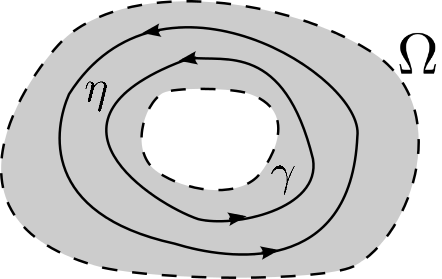
\includegraphics[width=0.3\textwidth]{25.png}
  \end{center}
\end{wrapfigure}



 $\varphi_{\alpha}\in\mathcal{H}(  \Omega)$  (onde $\varphi_{\alpha}(z)=(z-\alpha)^{-1}$ 

$\forall z\in\Omega$) e $\left[  7\right]$ resulta pelo Teor. 5.7,


\indent por $\left[  1\right]$ e $\left[  4\right]$ (do início deste

 Cap. 7).

\bigskip

(b) \ Na figura 1 ao lado, as \textit{CSDF}


$\gamma$ e $\eta$ em $\Omega$ são $\Omega$-homólogas. De

% IMAGEM 26
\begin{wrapfigure}{r}{0.4\textwidth}
  \begin{center}
    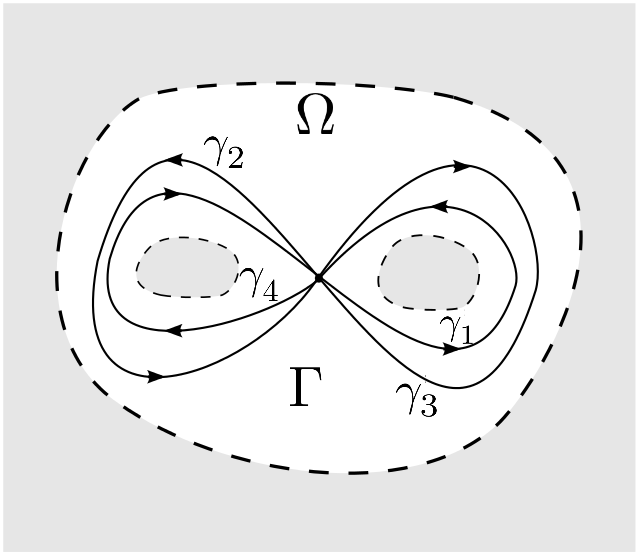
\includegraphics[width=0.4\textwidth]{26.png}
  \end{center}
\end{wrapfigure}





fato, se $\alpha\notin\Omega$ e $\alpha$  "está no buraco"


de $\Omega$ então \textsc{I}nd$_{\gamma}(  \alpha)=$\textsc{I}nd$_{\eta}(  \alpha)  =1.$

Se $\alpha\notin\Omega$ e $\alpha$ não está no buraco então

\textsc{I}nd$_{\gamma}(  \alpha)  =$\textsc{I}nd$_{\eta}(\alpha)  =0.$ Se $\Gamma:=\gamma-\eta$

resulta \textsc{I}nd$_{\Gamma}(\alpha)\!=0$ para

 cada $\alpha\notin\Omega.$\\


(c) \ Na figura 2 ao lado (a parte hachu-

rada aqui é $\complement\Omega$) consideremos o ciclo

$\Gamma=\gamma_{1}+\gamma_{2}+\gamma_{3}+\gamma_{4}$ em $\Omega$ que é homó-

logo a $0.$ De fato, se $\alpha\notin\Omega$ e $\alpha$ está no

buraco da direita (resp. esquerda) \ en-

tão \textsc{I}nd$_{\Gamma}(  \alpha)  =$\textsc{I}nd$_{\gamma_{1}}(  \alpha)  +$\textsc{I}nd$_{\gamma_{3}}(\alpha)  =$

$1+(  -1)  =0$ (resp. \textsc{I}nd$_{\Gamma}(  \alpha)= $\textsc{I}nd$_{\gamma_{2}}(  \alpha)  +$

\textsc{I}nd$_{\gamma_{3}}(  \alpha)  =1+(  -1)  =0$) e obviamente

\textsc{I}nd$_{\Gamma}(  \alpha)  =0$ se $\alpha$ está na componente

conexa ilimitada de $\complement\Omega$ pois neste ca-

so temos \textsc{I}nd$_{\gamma_{i}}(  \alpha)  =0$ \ para cada

$i=1,2,3,4.$\\

\bigskip

\textbf{Teorema 7.1 \ }(Cauchy) \ \textit{Sejam} $\Omega$\textit{\ um aberto não vazio de }$\mathbb{C}$\textit{\ e }

$f\in\mathcal{H}(  \Omega)  $, \textit{então valem as duas
asserções seguintes:}

(1%
%TCIMACRO{\U{ba}}%
%BeginExpansion
${{}^o}$%
%EndExpansion
) \ \textit{Se }$\Gamma$ \textit{é um ciclo em }$\Omega$ \textit{tal que}

\bigskip

$(  7.1.1)  $ \ \ \ \ \ \ \ \ \ \ \ \textsc{I}nd$_{\Gamma}(
\alpha)  =0$ \ \ \ \ \ $\forall$ \ \ \ \ $\alpha\notin\Omega$ \ \ (i.e.
\ $\Gamma\overset{\Omega}{\backsim}0$)

\bigskip

\textit{então}

\bigskip

$(  7.1.2)  $ \ \ \ \ \ \ \ \ \ \ \ $f(  z)
.$\textsc{I}nd$_{\Gamma}(  z)  =%
%TCIMACRO{\QDABOVE{1pt}{1}{2\pi i}}%
%BeginExpansion
\genfrac{}{}{1pt}{0}{1}{2\pi i}%
%EndExpansion
\underset{\Gamma}{%
%TCIMACRO{\dint }%
%BeginExpansion
{\displaystyle\int}
%EndExpansion
}%
%TCIMACRO{\QDABOVE{1pt}{f(  w)  dw}{w-z}}%
%BeginExpansion
\genfrac{}{}{1pt}{0}{f(  w)  dw}{w-z}%
%EndExpansion
$ \ \ \ \ \ \ \ $\forall$ \ \ \ $z\in\Omega\backslash\Gamma^{\ast}$

\bigskip\textit{e}

$(  7.1.3)  $ \ \ \ \ \ \ \ \ \ \ \ \ \ $\underset{\Gamma}{%
%TCIMACRO{\dint }%
%BeginExpansion
{\displaystyle\int}
%EndExpansion
}f(  z)  dz=0.$

\bigskip(2%
%TCIMACRO{\U{ba}}%
%BeginExpansion
${{}^o}$%
%EndExpansion
) \ \textit{Se }$\Gamma_{1}$ \textit{e }$\Gamma_{2\text{ }}$ \textit{são
dois ciclos em }$\Omega$ \textit{tais que}

\bigskip

$(  7.1.4)  $ \ \ \ \ \ \ \ \ \ \ \textsc{I}nd$_{\Gamma_{1}}(
\alpha)  =$\textsc{I}nd$_{\Gamma_{2}}(  \alpha)  $
\ \ \ \ \ $\forall$ \ \ $\alpha\notin\Omega$ \ \ \ (i.e. $\Gamma_{1}%
\overset{\Omega}{\backsim}\Gamma_{2}$)

\bigskip

\textit{então}

$(  7.1.5)  $ \ \ \ \ \ \ \ \ \ \ \ \ \ \ \ \ \ \ \ $\underset
{\Gamma_{1}}{%
%TCIMACRO{\dint }%
%BeginExpansion
{\displaystyle\int}
%EndExpansion
}f(  z)  dz=\underset{\Gamma_{2}}{%
%TCIMACRO{\dint }%
%BeginExpansion
{\displaystyle\int}
%EndExpansion
}f(  z)  dz.$

\bigskip

\textbf{Observação: \ }Já vimos no Exemplo (a) precedente que se
$\Omega=%
%TCIMACRO{\U{2102} }%
%BeginExpansion
\mathbb{C}
%EndExpansion
$ então

$(  7.1.1)  $ vale para cada ciclo $\Gamma$ em $\Omega=%
%TCIMACRO{\U{2102} }%
%BeginExpansion
\mathbb{C}
%EndExpansion
.$ Mas é pertinente observar que \textit{é}

\textit{inútil} provar o Teor. 7.1 no caso $\Omega=%
%TCIMACRO{\U{2102} }%
%BeginExpansion
\mathbb{C}
%EndExpansion
$ pois isto é imediato a partir do que

já foi feito. De fato, $\Omega=%
%TCIMACRO{\U{2102} }%
%BeginExpansion
\mathbb{C}
%EndExpansion
$ sendo um aberto convexo, a parte (1%
%TCIMACRO{\U{ba}}%
%BeginExpansion
${{}^o}$%
%EndExpansion
) do Teor.

7.1 resulta do Teor. 5.7, 5.8 e de $\left[  1\right]  $ (Ver início deste
Cap. 7). A parte (2%
%TCIMACRO{\U{ba}}%
%BeginExpansion
${{}^o}$%
%EndExpansion
)

do Teor. 7.1 (em qualquer caso $\Omega=%
%TCIMACRO{\U{2102} }%
%BeginExpansion
\mathbb{C}
%EndExpansion
$ ou $\Omega\neq%
%TCIMACRO{\U{2102} }%
%BeginExpansion
\mathbb{C}
%EndExpansion
$) é, como veremos, con-

sequência trivial da parte (1%
%TCIMACRO{\U{ba}}%
%BeginExpansion
${{}^o}$%
%EndExpansion
). \textit{Na prova do }\ Teor. 7.1 \textit{podemos portanto }

\textit{supor }$\Omega\neq%
%TCIMACRO{\U{2102} }%
%BeginExpansion
\mathbb{C}
%EndExpansion
.$

\bigskip

A prova que segue do Teor. 7.1 é devida a John D. Dixon, Proc. Am. Math.

Soc., Vol. 29, p. 625-626 (1971).

\bigskip

\textbf{Prova \ \ }(1%
%TCIMACRO{\U{ba}}%
%BeginExpansion
${{}^o}$%
%EndExpansion
) \ Seja $\ \Gamma=\underset{i=1}{\overset{\nu}{%
%TCIMACRO{\dsum }%
%BeginExpansion
{\displaystyle\sum}
%EndExpansion
}}n_{i}\gamma_{i}.$ Pelo Lema 6.1, a função $g:\Omega\times
\Omega\rightarrow%
%TCIMACRO{\U{2102} }%
%BeginExpansion
\mathbb{C}
%EndExpansion
$

definida por

\bigskip

\ \ \ \ \ \ \ \ \ \ \ \ \ \ \ \ $g(  z,w)  =\left\{
\begin{array}
[c]{c}%
(  w-z)  ^{-1}.\left[  f(  w)  -f(  z)
\right]  \text{ },\text{ \ se \ }w\neq z\\
\\
f^{\prime}(  z)  \text{ \ },\text{ \ se \ }w=z\text{
\ \ \ \ \ \ \ \ \ \ \ \ \ \ \ \ \ \ \ \ \ \ \ \ \ \ \ \ \ }%
\end{array}
\right.  $

\bigskip

é contínua em $\Omega\times\Omega.$ Em consequência podemos definir

\bigskip

\ \ \ \ \ \ \ \ \ \ \ \ \ \ \ \ \ \ $h(  z)  :=%
%TCIMACRO{\QDABOVE{1pt}{1}{2\pi i}}%
%BeginExpansion
\genfrac{}{}{1pt}{0}{1}{2\pi i}%
%EndExpansion
\underset{\Gamma}{%
%TCIMACRO{\dint }%
%BeginExpansion
{\displaystyle\int}
%EndExpansion
}g(  z,w)  dw$ \ \ \ \ \ $\forall$ \ \ $z\in\Omega$

e como

\ \ \ \ \ \ \ \ \ \ \ \ \ \ \ \ \ $g(  z,w)  =(  w-z)
^{-1}.\left[  f(  w)  -f(  z)  \right]  $
\ \ \ \ $\forall$ \ \ $(  z,w)  \in(  \Omega\backslash
\Gamma^{\ast})  \times\Gamma^{\ast}$

resulta que

\bigskip

$(  7.1.6)  $ \ \ \ \ \ $\left\vert
\begin{array}
[c]{c}%
h(  z)  =%
%TCIMACRO{\QDABOVE{1pt}{1}{2\pi i}}%
%BeginExpansion
\genfrac{}{}{1pt}{0}{1}{2\pi i}%
%EndExpansion
\underset{\Gamma}{%
%TCIMACRO{\dint }%
%BeginExpansion
{\displaystyle\int}
%EndExpansion
}%
%TCIMACRO{\QDABOVE{1pt}{f(  w)  dw}{w-z}}%
%BeginExpansion
\genfrac{}{}{1pt}{0}{f(  w)  dw}{w-z}%
%EndExpansion
-%
%TCIMACRO{\QDABOVE{1pt}{1}{2\pi i}}%
%BeginExpansion
\genfrac{}{}{1pt}{0}{1}{2\pi i}%
%EndExpansion
\underset{\Gamma}{%
%TCIMACRO{\dint }%
%BeginExpansion
{\displaystyle\int}
%EndExpansion
}%
%TCIMACRO{\QDABOVE{1pt}{f(  z)  dw}{w-z}}%
%BeginExpansion
\genfrac{}{}{1pt}{0}{f(  z)  dw}{w-z}%
%EndExpansion
=\text{ \ }\\
\\
=%
%TCIMACRO{\QDABOVE{1pt}{1}{2\pi i}}%
%BeginExpansion
\genfrac{}{}{1pt}{0}{1}{2\pi i}%
%EndExpansion
\underset{\Gamma}{%
%TCIMACRO{\dint }%
%BeginExpansion
{\displaystyle\int}
%EndExpansion
}%
%TCIMACRO{\QDABOVE{1pt}{f(  w)  }{w-z}}%
%BeginExpansion
\genfrac{}{}{1pt}{0}{f(  w)  }{w-z}%
%EndExpansion
-f(  z)  .\text{\textsc{I}nd}_{\Gamma}(  z)  \text{
\ \ \ \ }\forall\text{ \ \ }z\in\Omega\backslash\Gamma^{\ast}\\
\end{array}
\right.  $

\bigskip

e portanto, provar $(  7.1.2)  $ equivale a mostrar que $h(
z)  =0$ para cada

$z\in\Omega\backslash\Gamma^{\ast}.$ Na realidade vamos mostrar que

\bigskip

$(  7.1.7)  $ \ \ \ \ \ \ \ \ \ \ \ \ \ \ \ \ \ \ $h(
z)  =0$ \ \ \ \ \ $\forall$ \ \ $z\in\Omega.$

\bigskip

Comecemos provando que $h\in\mathcal{H}(  \Omega)  .$ Como
$g\in\mathcal{C}(  \Omega\times\Omega,%
%TCIMACRO{\U{2102} }%
%BeginExpansion
\mathbb{C}
%EndExpansion
)  $ resulta que

$g$ é uniformemente contínua sobre cada $K\subset\subset\Omega
\times\Omega,$ donde se segue que,

dados $\zeta\in\Omega$ e $\varepsilon>0$ arbitrário, se $\overline{D}%
_{r}(  \zeta)  \subset\subset\Omega$ então $\overline{D}%
_{r}(  \zeta)  \times\Gamma^{\ast}\subset\subset\Omega\times\Omega$

o que implica que $g|\overline{D}_{r}(  \zeta)  \times\Gamma^{\ast
}$ é uniformemente contínua. Em particular,

existe $\delta\in]0,r[$ tal que

\bigskip

\ \ \ \ \ \ \ \ \ $\left\vert z-\zeta\right\vert \leq\delta\implies\left\vert
g(  z,w)  -g(  \zeta,w)  \right\vert \leq%
%TCIMACRO{\QDABOVE{1pt}{2\pi\varepsilon}{\underset{i=1}{\overset{\nu}{\dsum
%}}\left\vert \eta_{i}\right\vert \left\vert \gamma_{i}\right\vert }}%
%BeginExpansion
\genfrac{}{}{1pt}{0}{2\pi\varepsilon}{\underset{i=1}{\overset{\nu
}{{\displaystyle\sum}}}\left\vert \eta_{i}\right\vert \left\vert \gamma
_{i}\right\vert }%
%EndExpansion
$ \ \ \ \ \ $\forall$ \ \ \ $w\in\Gamma^{\ast}$

donde:

\bigskip\ \ \ \ \ \ \ 

\ $\left\vert z-\zeta\right\vert \leq\delta\implies\left\vert h(
z)  -h(  \zeta)  \right\vert \leq%
%TCIMACRO{\QDABOVE{1pt}{1}{2\pi}}%
%BeginExpansion
\genfrac{}{}{1pt}{0}{1}{2\pi}%
%EndExpansion
\overset{\nu}{\underset{i=1}{%
%TCIMACRO{\dsum }%
%BeginExpansion
{\displaystyle\sum}
%EndExpansion
}}\left\vert n_{i}\right\vert \underset{\gamma_{i}}{%
%TCIMACRO{\dint }%
%BeginExpansion
{\displaystyle\int}
%EndExpansion
}\left\vert g(  z,w)  -g(  \zeta,w)  \right\vert
\left\vert dw\right\vert \leq\varepsilon$

\bigskip

o que mostra que

\bigskip

$(  7.1.8)  $
\ \ \ \ \ \ \ \ \ \ \ \ \ \ \ \ \ \ \ \ \ \ \ \ \ \ \ \ \ \ \ \ \ \ \ \ \ \ \ $h\in
\mathcal{C}(  \Omega)  $ $.$

\bigskip

Fixemos $w\in\Omega$ arbitário e seja $\psi_{w}:z\in\Omega\longmapsto
g(  z,w)  \in%
%TCIMACRO{\U{2102} }%
%BeginExpansion
\mathbb{C}
%EndExpansion
,$ então como

$g\in\mathcal{C}(  \Omega\times\Omega)  $ é claro que $\psi
_{w}\in\mathcal{C}(  \Omega)  .$ Por outro lado, é claro pela defini-

ção de $g$ que $\psi_{w}\in\mathcal{H}(  \Omega\backslash\left\{
w\right\}  )  ,$ pois $z\longmapsto f(  w)  -f(
z)  $\ e $z\longmapsto w-z$ \ são

holomorfas e o denominador não é nulo em $\Omega\backslash\left\{
w\right\}  .$ Logo pelo exerc.

(5.14) temos $\psi_{w}\in\mathcal{H}(  \Omega)  ,$ o que prova que

\bigskip

$(  7.1.9)  $ \ \ \ \ \ \ \ \ \ \ \ \ \ \ $\psi_{w}\in
\mathcal{H}(  \Omega)  $ \ \ \ \ $\forall$ \ \ $w\in\Omega$ $.$

\bigskip

Para provar que $h\in\mathcal{H}(  \Omega)  ,$ por $(
7.1.8)  $ e pelo teorema de Morera (Teor.

5.17) basta provar que se $\Delta$ é um tri\^{a}ngulo fechado
arbitrário contido em

$\Omega$ então

\bigskip

$(  7.1.10)  $
\ \ \ \ \ \ \ \ \ \ \ \ \ \ \ \ \ \ \ \ \ \ \ \ $\underset{\partial\Delta}{%
%TCIMACRO{\dint }%
%BeginExpansion
{\displaystyle\int}
%EndExpansion
}h(  z)  dz=0$ \ $,$

\bigskip

o que é uma consequência imediata do teorema de Fubini, do teorema de

Cauchy para um tri\^{a}ngulo (Lema 5.6) e de $(  7.1.9)  .$ De fato,

\bigskip

$\ \ \underset{\partial\Delta}{%
%TCIMACRO{\dint }%
%BeginExpansion
{\displaystyle\int}
%EndExpansion
}h(  z)  dz=\underset{\partial\Delta}{%
%TCIMACRO{\dint }%
%BeginExpansion
{\displaystyle\int}
%EndExpansion
}\left\{
%TCIMACRO{\QDABOVE{1pt}{1}{2\pi i}}%
%BeginExpansion
\genfrac{}{}{1pt}{0}{1}{2\pi i}%
%EndExpansion
\underset{\Gamma}{%
%TCIMACRO{\dint }%
%BeginExpansion
{\displaystyle\int}
%EndExpansion
}g(  z,w)  dw\right\}  dz=%
%TCIMACRO{\QDABOVE{1pt}{1}{2\pi i}}%
%BeginExpansion
\genfrac{}{}{1pt}{0}{1}{2\pi i}%
%EndExpansion
\underset{\Gamma}{%
%TCIMACRO{\dint }%
%BeginExpansion
{\displaystyle\int}
%EndExpansion
}(  \underset{\partial\Delta}{%
%TCIMACRO{\dint }%
%BeginExpansion
{\displaystyle\int}
%EndExpansion
}g(  z,w)  dz)  dw=$

\bigskip

$=%
%TCIMACRO{\QDABOVE{1pt}{1}{2\pi i}}%
%BeginExpansion
\genfrac{}{}{1pt}{0}{1}{2\pi i}%
%EndExpansion
\underset{\Gamma}{%
%TCIMACRO{\dint }%
%BeginExpansion
{\displaystyle\int}
%EndExpansion
}(  \underset{\partial\Delta}{%
%TCIMACRO{\dint }%
%BeginExpansion
{\displaystyle\int}
%EndExpansion
\psi_{w}}(  z)  dz)  dw=0$ $,$ já que por $(
7.1.9)  $ e pelo Lema 5.6 temos

\bigskip

$\underset{\partial\Delta}{%
%TCIMACRO{\dint }%
%BeginExpansion
{\displaystyle\int}
%EndExpansion
}\psi_{w}(  z)  dz=0$ \ \ \ \ $\forall$ \ \ $w\in\Omega.$ Desta
forma, provamos $(  7.1.10)  $ e portanto

\bigskip

que $h\in\mathcal{H}(  \Omega)  .$ Seja agora

\bigskip\ \ \ \ \ \ \ \ \ \ \ \ \ \ \ \ \ \ \ \ \ \ \ \ \ \ \ \ $\Omega
_{1}:=\left\{  z\in%
%TCIMACRO{\U{2102} }%
%BeginExpansion
\mathbb{C}
%EndExpansion
\text{ }|\text{ \textsc{I}nd}_{\Gamma}(  z)  =0\right\}  $ $,$

\bigskip

é claro (pelo Teor. 5.2) que $\Omega_{1}$ é aberto e como por
definição de $\Omega_{1}$ temos

$\Omega_{1}\cap\Gamma^{\ast}=\varnothing,$ o Teor. 4.3 implica que a função

\ \ \ \ \ \ \ \ \ \ \ \ \ 

\ \ \ \ \ \ \ \ \ \ \ \ \ \ \ \ \ \ \ $h_{1}:z\in\Omega_{1}\longmapsto%
%TCIMACRO{\QDABOVE{1pt}{1}{2\pi i}}%
%BeginExpansion
\genfrac{}{}{1pt}{0}{1}{2\pi i}%
%EndExpansion
\underset{\Gamma}{%
%TCIMACRO{\dint }%
%BeginExpansion
{\displaystyle\int}
%EndExpansion
}%
%TCIMACRO{\QDABOVE{1pt}{f(  w)  dw}{w-z}}%
%BeginExpansion
\genfrac{}{}{1pt}{0}{f(  w)  dw}{w-z}%
%EndExpansion
\in%
%TCIMACRO{\U{2102} }%
%BeginExpansion
\mathbb{C}
%EndExpansion
$

é analítica em $\Omega_{1}.$ Como estamos supondo $\Omega\neq%
%TCIMACRO{\U{2102} }%
%BeginExpansion
\mathbb{C}
%EndExpansion
,$ \ isto é $\complement\Omega\neq\varnothing,$ e a

hipótese $(  7.1.1)  $ implica $\complement\Omega\subset
\Omega_{1},$ resultam as duas asserções seguintes:

\bigskip

$\
%TCIMACRO{\U{2102} }%
%BeginExpansion
\mathbb{C}
%EndExpansion
=\Omega\cup\complement\Omega\subset\Omega\cup\Omega_{1}=%
%TCIMACRO{\U{2102} }%
%BeginExpansion
\mathbb{C}
%EndExpansion
$ \ \ \ \ e \ \ \ \ \ $\Omega_{1}\neq\varnothing$ \ \ \ (pois $\Omega
_{1}\supset\complement\Omega\neq\varnothing$).

\bigskip

Como $%
%TCIMACRO{\U{2102} }%
%BeginExpansion
\mathbb{C}
%EndExpansion
$ é conexo, as relações acima (junto ao fato óbvio:
$\Omega\neq\varnothing$) impli-

cam $\Omega_{1}\cap\Omega\neq\varnothing.$ De $(  7.1.6)  $ e das
definições de $\Omega_{1}$ e $h_{1}$ \ resulta

\ \ \ \ \ \ \ \ \ \ \ \ \ \ \ \ \ \ \ \ \ \ \ \ \ $h|\Omega\cap\Omega
_{1}=h_{1}|\Omega\cap\Omega_{1}$

o que permite definir uma função inteira

\ \ \ \ \ \ \ \ \ \ \ \ \ \ \ \ \ \ \ \ \ \ \ \ \ \ $\varphi:\Omega\cup
\Omega_{1}=%
%TCIMACRO{\U{2102} }%
%BeginExpansion
\mathbb{C}
%EndExpansion
\longrightarrow%
%TCIMACRO{\U{2102} }%
%BeginExpansion
\mathbb{C}
%EndExpansion
$

por $\varphi|\Omega:=h$ \ e \ $\varphi|\Omega_{1}:=h_{1}.$ Temos então
$\varphi\in\mathcal{H}(
%TCIMACRO{\U{2102} }%
%BeginExpansion
\mathbb{C}
%EndExpansion
)  .$

Se $V_{i}$ é a componente ilimitada de $\complement\gamma_{i}^{\ast}$
$(  i-1,2,\ldots,\nu)  $ então $V=\underset{i\leq1\leq\nu}{%
%TCIMACRO{\dbigcap }%
%BeginExpansion
{\displaystyle\bigcap}
%EndExpansion
}V_{i}$

é a componente ilimitada de $\complement\Gamma^{\ast},$ logo pelo Teor.
5.2 resulta que

$V\subset\Omega_{1},$ (portanto $\Omega_{1}$ é ilimitado) e então de
$\varphi|\Omega_{1}=h_{1}$ resulta (admi-

tindo a existência desses limites):

\bigskip

$(  7.1.11)  $ \ \ \ \ \ \ $\underset{\left\vert z\right\vert
\underset{z\in\Omega}{\rightarrow+\infty}}{\lim}\varphi(  z)
=\underset{\left\vert z\right\vert \underset{z\in\Omega_{1}}{\rightarrow
+\infty}}{\lim}h_{1}(  z)  $

\bigskip

Mostremos que $\underset{\left\vert z\right\vert \rightarrow+\infty}{\lim
}h_{1}(  z)  =0.$ De fato, dado $\varepsilon>0,$ vamos mostrar

\bigskip que existe $K>0$ tal que

\ \ \ \ \ \ \ \ \ \ \ \ \ \ \ \ \ \ \ \ \ \ \ \ \ \ \ \ \ $\left\vert
z\right\vert >K\implies\left\vert h_{1}(  z)  \right\vert
\leq\varepsilon$

Tomamos

\ \ \ \ \ \ \ \ \ \ \ \ \ \ \ \ \ \ \ \ $K>\sup\left\{
%TCIMACRO{\QDABOVE{1pt}{1}{\pi\varepsilon}}%
%BeginExpansion
\genfrac{}{}{1pt}{0}{1}{\pi\varepsilon}%
%EndExpansion
\underset{i=1}{\overset{\nu}{%
%TCIMACRO{\dsum }%
%BeginExpansion
{\displaystyle\sum}
%EndExpansion
}}\left\vert n_{i}\right\vert \left\vert \gamma_{i}\right\vert \left\Vert
f\right\Vert _{\gamma_{i}^{\ast}}\text{ \ },\text{ \ }2\text{ }\underset
{w\in\Gamma^{\ast}}{\sup}\left\vert w\right\vert \right\}  $ \ $.$

\bigskip

A desigualdade $K>2\underset{w\in\Gamma^{\ast}}{\sup}\left\vert w\right\vert $ implica

\bigskip

$\left\vert w-z\right\vert \geq\left\vert \left\vert w\right\vert -\left\vert
z\right\vert \right\vert =\left\vert z\right\vert -\left\vert w\right\vert
>K-\left\vert w\right\vert >K/2$ \ \ \ $\forall$ \ \ $\left\{
\begin{array}
[c]{c}%
w\in\Gamma^{\ast}\\
\left\vert z\right\vert >K
\end{array}
\right.  $

\bigskip

donde resulta para $\left\vert z\right\vert >K:$

\bigskip

$\ \ \ \ \ \left\vert h_{1}(  z)  \right\vert =\left\vert
%TCIMACRO{\QDABOVE{1pt}{1}{2\pi i}}%
%BeginExpansion
\genfrac{}{}{1pt}{0}{1}{2\pi i}%
%EndExpansion
\underset{i=1}{\overset{\nu}{%
%TCIMACRO{\dsum }%
%BeginExpansion
{\displaystyle\sum}
%EndExpansion
}}n_{i}\underset{\gamma_{i}}{%
%TCIMACRO{\dint }%
%BeginExpansion
{\displaystyle\int}
%EndExpansion
}%
%TCIMACRO{\QDABOVE{1pt}{f(  w)  dw}{w-z}}%
%BeginExpansion
\genfrac{}{}{1pt}{0}{f(  w)  dw}{w-z}%
%EndExpansion
\right\vert \leq%
%TCIMACRO{\QDABOVE{1pt}{1}{2\pi}}%
%BeginExpansion
\genfrac{}{}{1pt}{0}{1}{2\pi}%
%EndExpansion
\underset{i=1}{\overset{\nu}{%
%TCIMACRO{\dsum }%
%BeginExpansion
{\displaystyle\sum}
%EndExpansion
}}\left\vert n_{i}\right\vert \left\vert \underset{\gamma_{i}}{%
%TCIMACRO{\dint }%
%BeginExpansion
{\displaystyle\int}
%EndExpansion
}%
%TCIMACRO{\QDABOVE{1pt}{f(  w)  dw}{w-z}}%
%BeginExpansion
\genfrac{}{}{1pt}{0}{f(  w)  dw}{w-z}%
%EndExpansion
\right\vert \leq$

\bigskip

$\ \ \ \ \ \ \leq%
%TCIMACRO{\QDABOVE{1pt}{1}{2\pi}}%
%BeginExpansion
\genfrac{}{}{1pt}{0}{1}{2\pi}%
%EndExpansion
\underset{i=1}{\overset{\nu}{%
%TCIMACRO{\dsum }%
%BeginExpansion
{\displaystyle\sum}
%EndExpansion
}}\left\vert n_{i}\right\vert \underset{\gamma_{i}}{%
%TCIMACRO{\dint }%
%BeginExpansion
{\displaystyle\int}
%EndExpansion
}%
%TCIMACRO{\QDABOVE{1pt}{\left\vert f(  w)  \right\vert }{\left\vert
%w-z\right\vert }}%
%BeginExpansion
\genfrac{}{}{1pt}{0}{\left\vert f(  w)  \right\vert }{\left\vert
w-z\right\vert }%
%EndExpansion
\left\vert dw\right\vert \leq%
%TCIMACRO{\QDABOVE{1pt}{1}{2\pi}}%
%BeginExpansion
\genfrac{}{}{1pt}{0}{1}{2\pi}%
%EndExpansion
\underset{i=1}{\overset{\nu}{%
%TCIMACRO{\dsum }%
%BeginExpansion
{\displaystyle\sum}
%EndExpansion
}}\left\vert n_{i}\right\vert \underset{\gamma_{i}}{%
%TCIMACRO{\dint }%
%BeginExpansion
{\displaystyle\int}
%EndExpansion
}%
%TCIMACRO{\QDABOVE{1pt}{\left\Vert f\right\Vert _{\gamma_{i}^{\ast}}}{K/2}}%
%BeginExpansion
\genfrac{}{}{1pt}{0}{\left\Vert f\right\Vert _{\gamma_{i}^{\ast}}}{K/2}%
%EndExpansion
\left\vert dw\right\vert =$

\bigskip

$=%
%TCIMACRO{\QDABOVE{1pt}{1}{\pi K}}%
%BeginExpansion
\genfrac{}{}{1pt}{0}{1}{\pi K}%
%EndExpansion
\underset{i=1}{\overset{\nu}{%
%TCIMACRO{\dsum }%
%BeginExpansion
{\displaystyle\sum}
%EndExpansion
}}\left\vert n_{i}\right\vert \left\vert \gamma_{i}\right\vert \left\Vert
f\right\Vert _{\gamma_{i}^{\ast}}<\varepsilon$ \ , o que prova que
$\underset{\left\vert z\right\vert \underset{z\in\Omega_{1}}{\rightarrow
+\infty}}{\lim}h_{1}(  z)  =0$ \ e então

por (7.1.11) resulta

\bigskip

$(  7.1.12)  $ \ \ \ \ \ \ \ \ \ \ \ $\underset{\left\vert
z\right\vert \rightarrow+\infty}{\lim}\varphi(  z)  =0\ \ $e
\ portanto $\ \ \underset{\left\vert z\right\vert \rightarrow+\infty}{\lim
}\varphi(  z)  =0$

\ \ \ \ \ \ \ \ \ \ \ \ \ \ \ \ \ \ \ \ \ \ \ \ \ $\overset{z\in\Omega_{1}}{}%
$%
\ \ \ \ \ \ \ \ \ \ \ \ \ \ \ \ \ \ \ \ \ \ \ \ \ \ \ \ \ \ \ \ \ \ \ $\overset
{z\in%
%TCIMACRO{\U{2102} }%
%BeginExpansion
\mathbb{C}
%EndExpansion
}{}$\ \ \ \ \ \ \ \ \ \ \ \ \ \ 

\ \ \ \ \ \ \ \ \ \ \ \ \ \ \ \ \ \ \ \ \ \ \ \ \ \ \ \ \ \ \ \ \ \ \ \ \ \ \ \ \ \ \ \ \ \ \ \ \ \ \ \ \ \ \ \ \ \ \ \ \ \ \ \ \ \ \ 

Ora, $\varphi$ é inteira e então $(  7.1.12)  $ mostra que
$\varphi$ é limitada, logo pelo Corol.

5.12 (teor. de Louiville), resulta que $\varphi$ é constante, logo por
$(  7.1.12)  $

resulta que $\varphi=0.$ A relação $\varphi|\Omega=h,$ prova então
$(  7.1.7)  ,$ o que por

$(  7.1.6)  $ demonstra $(  7.1.2)  .$

Vamos provar $(  7.1.3)  $ a partir de $(  7.1.2)  .$
Seja $a\in\Omega\backslash\Gamma^{\ast}$ um ponto arbitrário,

então definimos

\ \ \ \ \ \ \ \ \ \ \ \ \ \ \ \ \ \ \ \ \ \ \ \ \ \ $F(  z)
:=(  z-a)  f(  z)  $ \ \ \ \ \ $\forall$ \ \ \ $z\in
\Omega$

É claro então que

\ \ \ \ \ \ \ \ \ \ \ \ \ \ \ \ \ \ \ \ \ \ \ \ \ \ \ \ \ \ $\left\{
\begin{array}
[c]{c}%
f(  z)  =%
%TCIMACRO{\QDABOVE{1pt}{F(  z)  }{z-a}}%
%BeginExpansion
\genfrac{}{}{1pt}{0}{F(  z)  }{z-a}%
%EndExpansion
\text{ \ \ \ \ }\forall\text{ \ \ \ }z\in\Gamma^{\ast}\text{ \ \ }\\
\\
F\in\mathcal{H}(  \Omega)  \text{
\ \ \ \ \ \ \ \ \ \ \ \ \ \ \ \ \ \ \ \ \ \ \ \ \ \ }%
\end{array}
\right.  $

\bigskip

Por $(  7.1.2)  $ aplicada à função $F$ temos:

\bigskip

$\ \ \ \ \ \ \
%TCIMACRO{\QDABOVE{1pt}{1}{2\pi i}}%
%BeginExpansion
\genfrac{}{}{1pt}{0}{1}{2\pi i}%
%EndExpansion
\underset{\Gamma}{%
%TCIMACRO{\dint }%
%BeginExpansion
{\displaystyle\int}
%EndExpansion
}f(  z)  dz=%
%TCIMACRO{\QDABOVE{1pt}{1}{2\pi i}}%
%BeginExpansion
\genfrac{}{}{1pt}{0}{1}{2\pi i}%
%EndExpansion
\underset{\Gamma}{%
%TCIMACRO{\dint }%
%BeginExpansion
{\displaystyle\int}
%EndExpansion
}%
%TCIMACRO{\QDABOVE{1pt}{F(  z)  }{z-a}}%
%BeginExpansion
\genfrac{}{}{1pt}{0}{F(  z)  }{z-a}%
%EndExpansion
dz=$\textsc{I}nd$_{\Gamma}(  a)  .F(  a)  =0$

\bigskip

pois $F(  a)  =0,$ o que prova $(  7.1.3)  .$

\bigskip

Finalmente, $(  7.1.5)  $ segue de $(  7.1.4)  $ e
$(  7.1.3)  $ aplicado ao ciclo

$\Gamma=\Gamma_{1}-\Gamma_{2}$, pois se $\alpha\notin\Omega$ então

\bigskip

\ \ \ \ \textsc{I}nd$_{\Gamma}(  \alpha)  =%
%TCIMACRO{\QDABOVE{1pt}{1}{2\pi i}}%
%BeginExpansion
\genfrac{}{}{1pt}{0}{1}{2\pi i}%
%EndExpansion
\underset{\Gamma}{%
%TCIMACRO{\dint }%
%BeginExpansion
{\displaystyle\int}
%EndExpansion
}%
%TCIMACRO{\QDABOVE{1pt}{dz}{z-a}}%
%BeginExpansion
\genfrac{}{}{1pt}{0}{dz}{z-a}%
%EndExpansion
=%
%TCIMACRO{\QDABOVE{1pt}{1}{2\pi i}}%
%BeginExpansion
\genfrac{}{}{1pt}{0}{1}{2\pi i}%
%EndExpansion
\underset{\Gamma_{1}}{%
%TCIMACRO{\dint }%
%BeginExpansion
{\displaystyle\int}
%EndExpansion
}%
%TCIMACRO{\QDABOVE{1pt}{dz}{z-\alpha}}%
%BeginExpansion
\genfrac{}{}{1pt}{0}{dz}{z-\alpha}%
%EndExpansion
-%
%TCIMACRO{\QDABOVE{1pt}{1}{2\pi i}}%
%BeginExpansion
\genfrac{}{}{1pt}{0}{1}{2\pi i}%
%EndExpansion
\underset{\Gamma_{1}}{%
%TCIMACRO{\dint }%
%BeginExpansion
{\displaystyle\int}
%EndExpansion
}%
%TCIMACRO{\QDABOVE{1pt}{dz}{z-\alpha}}%
%BeginExpansion
\genfrac{}{}{1pt}{0}{dz}{z-\alpha}%
%EndExpansion
=$

\ \ 

\ \ \ $=$\textsc{I}nd$_{\Gamma_{1}}(  \alpha)  -$\textsc{I}%
nd$_{\Gamma_{2}}(  \alpha)  =0$ \ \ por $(  7.1.4)  ,$
isto é\ \ \ 

$\ \ \ \ \ \ \ \ \ \ \ \ \ \ \ \ \ \ \ \ \ $

$\ \ \ \ \ \ \ \ \ \ \ \ \ \ \ \ \ \ \ \ \ \ \ \ \ $\textsc{I}nd$_{\Gamma
}(  \alpha)  =0$ $\ \ \ \ \forall$ \ \ $\ \alpha\notin\Omega$

portanto por $(  7.1.3)  $ temos:

\bigskip

\ \ \ \ \ \ \ \ \ \ \ \ \ $0=\underset{\Gamma}{%
%TCIMACRO{\dint }%
%BeginExpansion
{\displaystyle\int}
%EndExpansion
}f(  z)  dz=\underset{\Gamma_{1}}{%
%TCIMACRO{\dint }%
%BeginExpansion
{\displaystyle\int}
%EndExpansion
}f(  z)  dz-\underset{\Gamma_{2}}{%
%TCIMACRO{\dint }%
%BeginExpansion
{\displaystyle\int}
%EndExpansion
}f(  z)  dz$ $.$ \ 

\bigskip

Observe que no caso $\Omega=%
%TCIMACRO{\U{2102} }%
%BeginExpansion
\mathbb{C}
%EndExpansion
$ já vimos que (1%
%TCIMACRO{\U{ba}}%
%BeginExpansion
${{}^o}$%
%EndExpansion
) vale e, em particular, $(  7.1.3)  $

é válida o que implica a identidade acima, que prova $(
7.1.5)  $ neste caso. $\square$

\bigskip

\textbf{Observação:} \ O Teor. 7.1 (1%
%TCIMACRO{\U{ba}}%
%BeginExpansion
${{}^o}$%
%EndExpansion
) generaliza o teor. de Cauchy num aberto

convexo (Teor. 5.7) e \ o teor. de representação integral de Cauchy (Teor.

5.8). De fato, se $\gamma$ é uma \textit{CSDF} num aberto convexo
$\Omega\neq%
%TCIMACRO{\U{2102} }%
%BeginExpansion
\mathbb{C}
%EndExpansion
$ \ e $\ \alpha\notin\Omega$

então aplicando o Teor. 5.7 à função holomorfa $\varphi
_{\alpha}(  z)  =(  z-\alpha)  ^{-1}$ $(
z\in\Omega)  $

resulta \textsc{I}nd$_{\gamma}(  \alpha)  =0,$ o que mostra que a
hipótese $(  7.1.1)  $ do Teor. 7.1

está satisfeita para cada ciclo em $\Omega$ se $\Omega$ é convexo.

\bigskip

Antes de introduzir o conceito de homotopia que vai nos conduzir ao con-

ceito fundamental de aberto simplesmente conexo além de fornecer uma

importante classe de exemplos de holomologia, vamos apresentar uma

consequência extremamente importante do Teor. 7.1 que mostra como o

cálculo de integrais ao longo de um ciclo "complicado "se reduz ao cálculo

de integrais sobre "pequenos círculos ". \textit{Este resultado mostra
também a }

\textit{razão pela qual era natural definir cadeias do modo como fizemos,
}\ isto é,

como combinações lineares formais de \textit{CSDF} com coeficientes
$\underline{\text{inteiros}}$.

Com a terminologia que será introduzida no Cap. 8 o resultado seguinte

será chamado "Teorema dos resíduos".

\bigskip

\textbf{Corolário 7.2 \ }\textit{Sejam }$\Omega$ \textit{um aberto não
vazio de }$%
%TCIMACRO{\U{2102} }%
%BeginExpansion
\mathbb{C}
%EndExpansion
,$ $F=\left\{  a_{1},a_{2\text{ }},\ldots,\text{ }a_{m}\right\}  $

\textit{um conjunto finito de pontos de }$\Omega,$ $f\in\mathcal{H}(
\Omega\backslash F)  $ \textit{e }$\Gamma$\textit{\ um ciclo em }%
$\Omega$ \ \textit{tal que}

\ \ \ \ \ \ \ \ \ \ \ \ \ \ \ \ \ \ \ \ \ \ \ \textsc{I}nd$_{\Gamma}(
\alpha)  =0$ \ \ \ \ $\forall$ \ \ \ $\alpha\notin\Omega$
\ \ \ \ \ \ $(  \text{i.e. \ }\Gamma\overset{\Omega}{\backsim}0)  $ .

\textit{Seja }$\gamma_{k}:t\in\left[  0,2\pi\right]  \longmapsto a_{k}%
+r_{k}e^{it}\in%
%TCIMACRO{\U{2102} }%
%BeginExpansion
\mathbb{C}
%EndExpansion
$ \ \textit{o círculo orientado positivamente de}

\textit{centro }$a_{k}$ \textit{e raio }$r_{k}$\textit{\ para cada }$k=1,$
$\ldots,$ $m.$ \textit{Indiquemos com }$D_{k}$ \textit{o disco }

\textit{aberto }$D_{r_{k}}(  a_{k})  $ \textit{e vamos supor ainda
que os} $r_{k}$ \textit{são suficientemente peque-}

\textit{nos de modo que:}

(1%
%TCIMACRO{\U{ba}}%
%BeginExpansion
${{}^o}$%
%EndExpansion
) \ $\overline{D}_{k}\subset\Omega$ \ \ \ \ $\forall$ \ \ $k=1,$ $\ldots, $
$m$ \ \ ; \ \ (2%
%TCIMACRO{\U{ba}}%
%BeginExpansion
${{}^o}$%
%EndExpansion
) \ $D_{k}\cap D_{j}=\varnothing$ \ \ \textit{se }$k\neq j$ $.$

\textit{Seja}

\ \ \ \ \ \ \ \ \ \ \ \ \ \ \ \ $n_{k}:=$ \textsc{I}nd$_{\Gamma}(
a_{k})  $ \ \ \ \ $\forall$ \ \ $k=1,2,$ $\ldots,$ $m$ $.$

(portanto $a_{k}\notin\Gamma^{\ast}$ \ $(  1\leq k\leq m)  $ donde
$\Gamma$ é um ciclo em $\Omega\backslash F.$)

\bigskip

\textit{Então:}

\ \ \ \ \ \ \ \ \ \ \ \ \ \ \ \ \ \ \ \ \ $\Gamma\overset{\Omega\backslash
F}{\backsim}\Sigma n_{k}\gamma_{k}$ \ \ 

\textit{e em particular}

\bigskip

\ \ \ \ \ \ \ \ \ \ \ \ \ \ \ \ \ \ $\underset{\Gamma}{%
%TCIMACRO{\dint }%
%BeginExpansion
{\displaystyle\int}
%EndExpansion
}f=\underset{1\leq k\leq m}{%
%TCIMACRO{\dsum }%
%BeginExpansion
{\displaystyle\sum}
%EndExpansion
}n_{k}\underset{\gamma_{k}}{%
%TCIMACRO{\dint }%
%BeginExpansion
{\displaystyle\int}
%EndExpansion
}f=\underset{\Sigma\eta_{k}\gamma_{k}}{%
%TCIMACRO{\dint }%
%BeginExpansion
{\displaystyle\int}
%EndExpansion
}f$

\bigskip

\textbf{Prova \ }Sejam $\Gamma_{1}:=\Gamma-\underset{k=1}{\overset{m}{%
%TCIMACRO{\dsum }%
%BeginExpansion
{\displaystyle\sum}
%EndExpansion
}}n_{k}\gamma_{k}$ \ e \ $\alpha\notin\Omega\backslash F.$\ Se $\alpha\notin
F,$ então $\alpha\notin\Omega$

portanto \textsc{I}nd$_{\gamma_{k}}(  \alpha)  =0$ para cada $k=1,
$ $\ldots,$ $m$ e portanto \textsc{I}nd$_{\Gamma_{1}}(  \alpha)  =$

$=$ \textsc{I}nd$_{\Gamma}(  \alpha)  -\overset{m}{\underset{k=1}{%
%TCIMACRO{\dsum }%
%BeginExpansion
{\displaystyle\sum}
%EndExpansion
}}n_{k}$ \textsc{I}nd$_{\gamma_{k}}(  \alpha)  =0-\underset
{k=1}{\overset{m}{%
%TCIMACRO{\dsum }%
%BeginExpansion
{\displaystyle\sum}
%EndExpansion
}}n_{k}0=0.$ Se $\alpha\in F,$ isto é, $\alpha=a_{j}$

para algum $j$ $(  1\leq j\leq m)  ,$ então \textsc{I}%
nd$_{\gamma_{k}}(  \alpha)  =\delta_{jk}$ \ $(  1\leq k\leq
m)  $ \ e então:

\textsc{I}nd$_{\Gamma_{1}}(  \alpha)  =$ \textsc{I}nd$_{\Gamma_{1}%
}(  a_{j})  =$ \textsc{I}nd$_{\Gamma}(  a_{j})
-\overset{m}{\underset{k=1}{%
%TCIMACRO{\dsum }%
%BeginExpansion
{\displaystyle\sum}
%EndExpansion
}}n_{k}\delta_{jk}=$\textsc{I}nd$_{\Gamma}(  a_{j})  -n_{j}=0$ \ por

hipótese. Em consequência provamos que

\ \ \ \ \ \ \ \ \ \ \ \ \ \ \ \ \ \ \ \ \ \ \ \textsc{I}nd$_{\Gamma_{1}%
}(  \alpha)  =0$ \ \ \ \ \ \ $\forall$ \ \ \ $\alpha\notin
\Omega\backslash F,$

isto é,

$\bigskip$ $\ \ \ \ \ \ \ \ \ \ \ \ \ \Gamma_{1}\overset{\Omega\backslash
F}{\backsim}0$ \ \ \ \ ou seja \ (por $\left[  8\right]  ,$ antes dos exemplos que

precedem o Teor. 7.1):

$\ \ \ \ \ \ \ \ \ \ \ \ \ \ \ \ \ \ \ \ \ \ \ \ \ \ \ \ \ \ \ \ \ \Gamma
\overset{\Omega\backslash F}{\backsim}\underset{1\leq k\leq m}{\text{ }%
%TCIMACRO{\dsum }%
%BeginExpansion
{\displaystyle\sum}
%EndExpansion
}n_{k}\gamma_{k}$ $.$

\bigskip Pelo Teor. 7.1 (2%
%TCIMACRO{\U{ba}}%
%BeginExpansion
${{}^o}$%
%EndExpansion
) resulta então $\underset{\Gamma}{%
%TCIMACRO{\dint }%
%BeginExpansion
{\displaystyle\int}
%EndExpansion
}f=\underset{k=1}{\overset{m}{%
%TCIMACRO{\dsum }%
%BeginExpansion
{\displaystyle\sum}
%EndExpansion
}}n_{k}\underset{\gamma_{k}}{%
%TCIMACRO{\dint }%
%BeginExpansion
{\displaystyle\int}
%EndExpansion
}f$ \ $.$ \ $\square$

\bigskip

Ilustramos o Corol. 7.2 com a figura

% IMAGEM 27
\begin{center}
  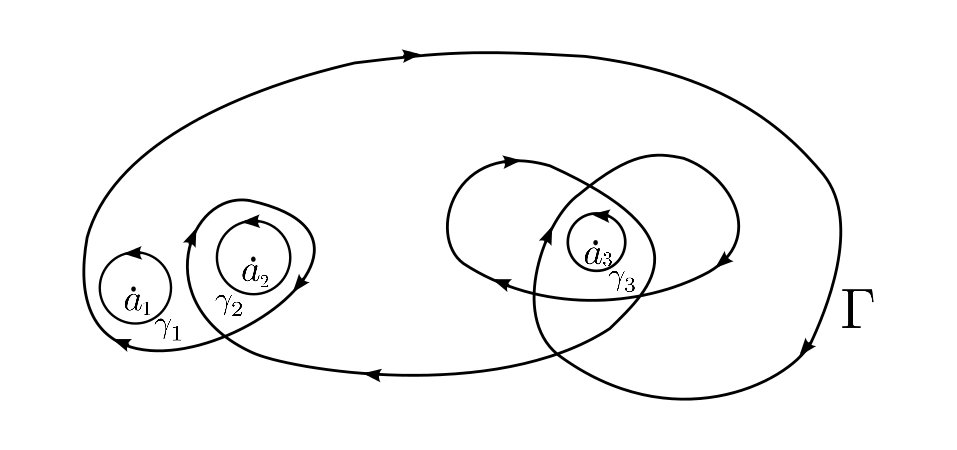
\includegraphics[width=0.7\textwidth]{27.png}
\end{center}

Como \textsc{I}nd$_{\Gamma}(  a_{1})  =-1,$ \textsc{I}nd$_{\Gamma
}(  a_{2})  =-2$ \ e \ \textsc{I}nd$_{\Gamma}(  a_{3})
=-3,$ o Corol. 7.2

implica $\Gamma\backsim-\gamma_{1}-2\gamma_{2}-3\gamma_{3}$ e portanto

\bigskip
\ \ \ \ \ \ \ \ \ \ \ \ \ \ \ \ \ \ \ \ \ \ \ \ \ \ \ \ \ \ \ \ $\underset
{\Gamma}{%
%TCIMACRO{\dint }%
%BeginExpansion
{\displaystyle\int}
%EndExpansion
}f=-\underset{\gamma_{1}}{%
%TCIMACRO{\dint }%
%BeginExpansion
{\displaystyle\int}
%EndExpansion
f}-2\underset{\gamma_{2}}{%
%TCIMACRO{\dint }%
%BeginExpansion
{\displaystyle\int}
%EndExpansion
}f-3\underset{\gamma_{3}}{%
%TCIMACRO{\dint }%
%BeginExpansion
{\displaystyle\int}
%EndExpansion
}f$

\bigskip

A seguir vamos introduzir e discutir brevemente um conceito topológico

que além do seu interesse próprio é importante do ponto de vista das

aplicações do teorema de Cauchy.

\bigskip

\textbf{Definição 7.3} \ Sejam \textsc{I}=$\left[  a,b\right]  $ um
intervalo compacto de $%
%TCIMACRO{\U{211d} }%
%BeginExpansion
\mathbb{R}
%EndExpansion
$ e $\Omega$ um aberto

de $%
%TCIMACRO{\U{2102} }%
%BeginExpansion
\mathbb{C}
%EndExpansion
.$

(1%
%TCIMACRO{\U{ba}}%
%BeginExpansion
${{}^o}$%
%EndExpansion
) \ Sejam $\gamma_{1}:$ \textsc{I} $\rightarrow\Omega$ e $\gamma_{2}:$
\textsc{I} $\rightarrow\Omega$ duas curvas em $\Omega$ tendo a mesma

origem e mesmo extremo (i.e. $\gamma_{1}(  a)  =\gamma_{2}(
a)  $ e $\gamma_{1}(  b)  =\gamma_{2}(  b)  $).
Diz-se que

$\gamma_{1}$ e $\gamma_{2}$ são \textit{homotópicas com extremos
fixos} (ou brevemente $\Omega$-\textit{HEF}) se

existe uma função contínua $h:$\textsc{I}$\times$\textsc{I}
$\rightarrow\Omega$ tal que:

(1) \ $h(  a,t)  =\gamma_{1}(  t)  $ \ \ $\forall$
\ \ $t\in$ \textsc{I} \ ;\ \ \ \ \ (3) \ $h(  s,a)  =\gamma
_{1}(  a)  =\gamma_{2}(  a)  $ \ \ \ \ $\forall$
\ \ $s\in$ \textsc{I}

(2) \ $h(  b,t)  =\gamma_{2}(  t)  $ \ \ $\forall$
\ \ $t\in$ \textsc{I} \ ; \ \ \ (4) \ $h(  s,b)  =\gamma_{1}(
b)  =\gamma_{2}(  b)  $ \ \ \ \ \ $\forall$ \ $s\in$
\textsc{I}

Diz-se também que $h$ é uma \textit{homotopia de} $\gamma_{1}$
\textit{a }$\gamma_{2}$ (ou uma \textit{deformação}

\textit{contínua de }$\gamma_{1}$ \textit{a }$\gamma_{2}$).

(2%
%TCIMACRO{\U{ba}}%
%BeginExpansion
${{}^o}$%
%EndExpansion
) \ Sejam $\gamma_{1}:$ \textsc{I} $\rightarrow\Omega$ e $\gamma_{2}:$
\textsc{I} $\rightarrow\Omega$ duas curvas fechadas em $\Omega.$ Diz-se

que $\gamma_{1}$ e $\gamma_{2}$ são $\Omega$-\textit{homotópicas como
curvas fechadas }(ou brevemente

$\Omega$-\textit{HCF}) se existe uma função contínua $h:$
\textsc{I}$\times$\textsc{I} $\rightarrow\Omega$ tal que, além das condi-

ções (1) e (2) acima, verifica a condição seguinte:

\bigskip

$(  3^{\prime})  $ \ \ \ \ \ \ \ \ \ \ \ \ \ \ $h(
s,a)  =h(  s,b)  $ \ \ \ \ $\forall$ \ \ $s\in$ \textsc{I}

\bigskip

Se $\gamma_{1}$ é constante dizemos que $\gamma_{1}$ é
\textit{homotópica a um ponto em }$\Omega.$

\bigskip

\textbf{Observação:} \ É possível definir homotopia de duas
curvas arbitrárias

no plano, i.e. sem extremos fixos, nós não o faremos pois não
será neces-

sário aqui (ver \cite{D}, pg 203).

\bigskip

O conceito de homotopia formaliza a ideia intuitiva de deformação con-

tínua de uma curva em outra. As duas figuras seguintes ilustram os casos

$\Omega$-\textit{HEF} e $\Omega$-\textit{HCF} respectivamente:

\bigskip

\textit{Caso }$\Omega$\textit{-HEF}

% IMAGEM 28
\begin{center}
  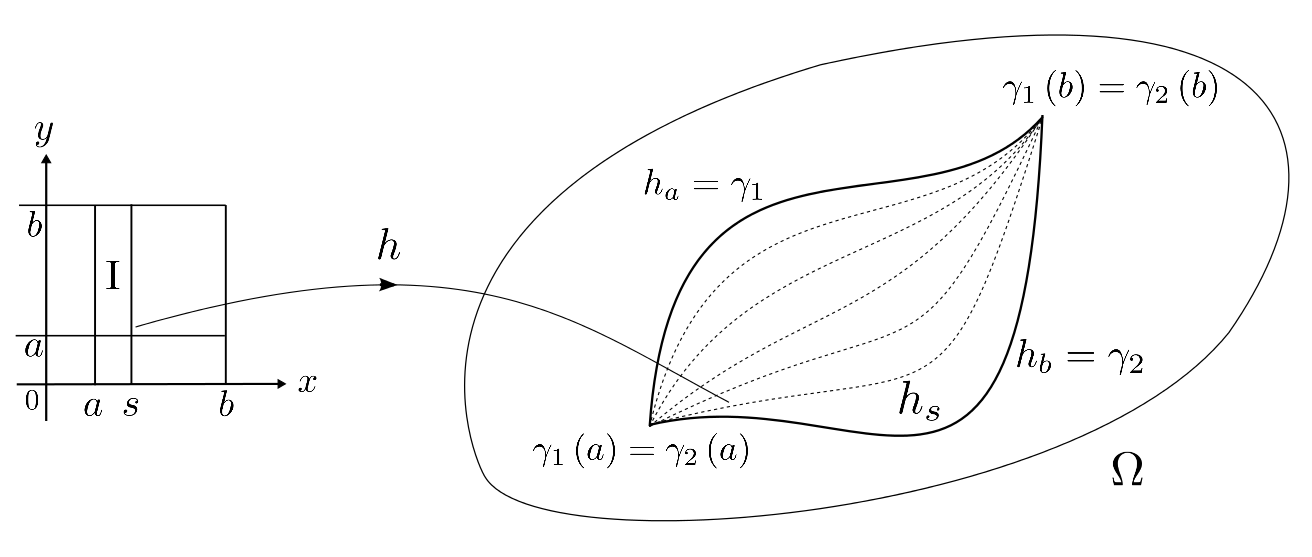
\includegraphics[width=0.9\textwidth]{28.png}
\end{center}

Para cada $s\in$ \textsc{I} a aplicação parcial $h_{s}:t\in$
\textsc{I} $\longmapsto h(  s,t)  \in\Omega$ é contínua

(pois $h$ o é) e as condições (3) e (4) mostram que $h_{s}$ tem
mesma origem

e mesmo extremo que $\gamma_{1}$ e $\gamma_{2}$ para cada $s\in$ \textsc{I}.
As condições (1) e (2)

mostram que $h_{a}=\gamma_{1}$ e $h_{b}=\gamma_{2}.$


Caso $\Omega-$\textit{HCF}

% IMAGEM 29
\begin{center}
  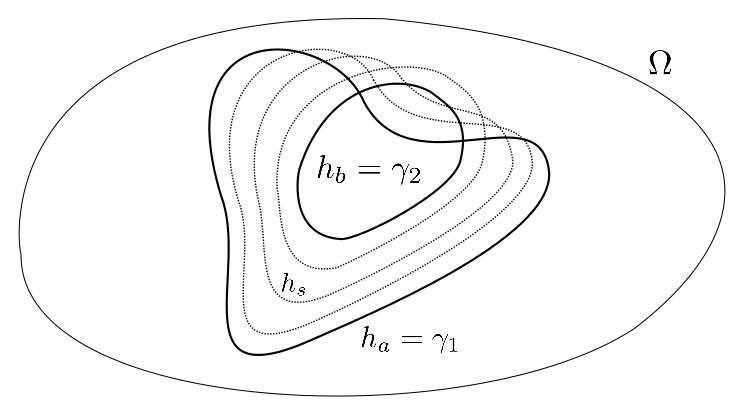
\includegraphics[width=0.7\textwidth]{29.png}
\end{center}

Como no caso anterior, para cada $s\in$ \textsc{I}\ a função parcial

$h_{s}:t\in$ \textsc{I} $\longmapsto h(  s,t)  \in\Omega$ \ é
contínua e a condição $(  3^{\prime})  $ mostra que
$h_{s}$

é uma curva fechada para cada $s\in$ \textsc{I.} As condições (1)
e (2) mos-

tram que $h_{a}=\gamma_{1}$\textsc{\ }e $\ h_{b}=\gamma_{2}.$

\bigskip

Falando intuitivamente, um \textit{aberto} \textit{simplesmente conexo }é
um aberto

conexo que "não tem buracos" e como a homotopia é a ferramenta mate-

mática que foi criada para "detectar buracos" podemos agora introduzir

naturalmente este conceito:

\bigskip

\textbf{Definição 7.4 \ }Um aberto não vazio $\Omega$ de $%
%TCIMACRO{\U{2102} }%
%BeginExpansion
\mathbb{C}
%EndExpansion
$ é dito \textit{simplesmente conexo}

se $\Omega$ é conexo e cada curva fechada $\gamma$ em $\Omega$ é
homotópica a um ponto

em $\Omega.$

\bigskip

\textbf{Exemplo \ }Um aberto $\Omega$ de $%
%TCIMACRO{\U{2102} }%
%BeginExpansion
\mathbb{C}
%EndExpansion
$ é dito $a$\textit{-estrelado }(onde $a\in\Omega$) se, para cada

$z\in\Omega$ tivermos $\left[  a,z\right]  ^{\ast}\subset\Omega$ \ (lembremos que

\ \ \ \ \ \ \ \ \ \ \ \ \ \ \ \ \ \ \ \ \ $\left[  a,z\right]  :t\in\left[
0,1\right]  \longmapsto(  1-t)  a+tz\in%
%TCIMACRO{\U{2102} }%
%BeginExpansion
\mathbb{C}
%EndExpansion
$).

É claro que um tal conjunto $\Omega$ é conexo (é trivial ver que
é conexo por poligo-

nais de dois lados) e $\Omega$ é simplesmente conexo pois se
$\gamma:\left[  0,1\right]  \rightarrow\Omega$ \ é

uma curva fechada em $\Omega$ então a função

\bigskip\ \ \ \ \ \ \ \ \ \ \ \ \ \ \ $h:(  s,t)  $\ $\in\left[
0,1\right]  $\ $\times\left[  0,1\right]  $\ $\longmapsto sa+(
1-s)  \gamma(  t)  \in%
%TCIMACRO{\U{2102} }%
%BeginExpansion
\mathbb{C}
%EndExpansion
$

define uma homotopia de $\gamma$ ao ponto $a.$ De fato, é claro que $h$
é contínua e

como $\gamma(  t)  \in\Omega$ \ \ $\forall$ \ \ $t\in\left[
0,1\right]  $ por hipótese e $\Omega$ é $a$-estrelado, resulta que

$\left[  a,\gamma(  t)  \right]  ^{\ast}$ está contido em
$\Omega$ para cada $t\in\left[  0,1\right]  ,$ isto é Im$(  h)
\subset\Omega.$ Além

disto, $h(  0,t)  =\gamma(  t)  $ \ \ $\forall$
\ \ $t\in\left[  0,1\right]  $ $,$ $h(  1,t)  =a$ \ \ $\forall$
\ $\ t\in\left[  0,1\right]  $ \ \ e $\ h(  s,0)  =$

$=sa+(  1-s)  \gamma(  0)  =sa+(  1-s)
\gamma(  t)  =h(  s,1)  $ \ \ $\forall$ \ \ $s\in\left[
0,1\right]  ,$ \ o que prova

as condições (1), (2) e $(  3^{\prime})  $ da $\Omega
$-\textit{HCF}.

Em particular, todo aberto convexo $\Omega$ (isto é, $\Omega$ é
$a$-estrelado \ \ $\forall$ \ \ $a\in\Omega$) \ é

simplesmente conexo.

\bigskip

O nosso próximo objetivo é demonstrar que se $\gamma_{1}$ e
$\gamma_{2}$ são duas \textit{CSDF} em

$\Omega,$ então

\bigskip\ \ \ \ \ \ \ \ \ \ \ \ \ \ \ \ \ \ \ \ $\left\vert
\begin{array}
[c]{c}%
\gamma_{1}\text{ e }\gamma_{2}\text{ são }\Omega\text{-\textit{HCF}
}\implies\gamma_{1}\overset{\Omega}{\backsim}\text{ }\gamma_{2}%
\text{\ \ \ \ \ \ \ \ \ \ \ \ \ \ \ \ \ \ \ \ }\\
\gamma_{1}\text{ é homotópica a um ponto em }\Omega\text{ }%
\implies\text{ }\gamma_{1}\overset{\Omega}{\backsim}0
\end{array}
\right.  $



\bigskip

e para isto precisamos do seguinte:

\bigskip



\textbf{Lema 7.5 \ }\textit{Sejam }$\gamma _{0}:\left[ 0,1\right]
\rightarrow 
%TCIMACRO{\U{2102} }%
%BeginExpansion
\mathbb{C}
%EndExpansion
$ \textit{e }$\gamma _{1}:\left[ 0,1\right] \rightarrow 
%TCIMACRO{\U{2102} }%
%BeginExpansion
\mathbb{C}
%EndExpansion
$ \textit{duas CSDF em }$%
%TCIMACRO{\U{2102} }%
%BeginExpansion
\mathbb{C}
%EndExpansion
,$

% IMAGEm 30
\begin{wrapfigure}{r}{0.3\textwidth}
  \begin{center}
    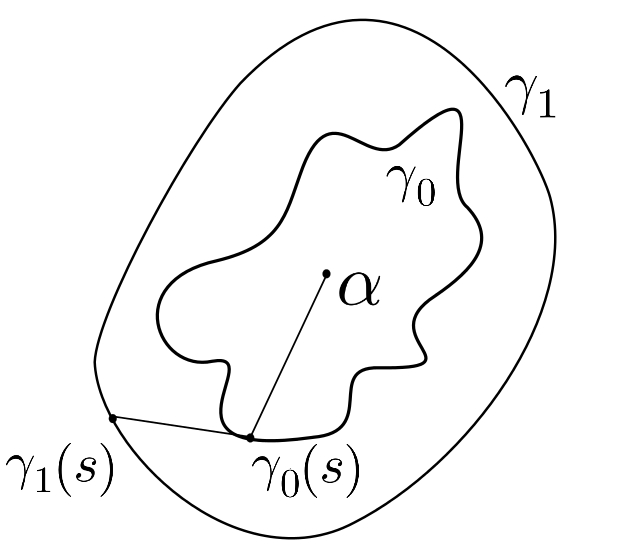
\includegraphics[width=0.3\textwidth]{30.png}
  \end{center}
\end{wrapfigure}
$\alpha \in 
%TCIMACRO{\U{2102} }%
%BeginExpansion
\mathbb{C}
%EndExpansion
$ \textit{e suponhamos que }

\bigskip

$(  7.5.1)  $ \ \ $\left\vert \gamma_{1}(  s)
-\gamma_{0}(  s)  \right\vert <\left\vert \alpha-\gamma_{0}(
s)  \right\vert $ \ \ $\forall$ $s\in\left[  0,1\right]  $

\bigskip

\textit{Então,}

\ \ \ \ \ \ \ \ \ \ \ \ \ \ \ \ \ \ \ \ \ \ \ \ \ \ \textsc{I}nd$_{\gamma_{1}%
}(  \alpha)  =$\textsc{I}nd$_{\gamma_{0}}(  \alpha)  $
$.$

\bigskip

\textbf{Prova \ }De $(  7.5.1)  $ resulta $\left\vert \alpha
-\gamma_{0}(  s)  \right\vert >0$

para cada $s\in\left[  0,1\right]  ,$ donde $\alpha\notin\gamma_{0}^{\ast} $
$.$ Se

$\alpha\in\gamma_{1}^{\ast}$ então \ $\exists$ $\ s_{0}\in\left[
0,1\right]  $ tal que \ $\alpha=\gamma_{1}(  s_{0})  $

e então por $(  7.5.1)  $

\ \ \ \ $\left\vert \alpha-\gamma_{0}(  s_{0})  \right\vert
=\left\vert \gamma_{1}(  s_{0})  -\gamma_{0}(  s_{0})
\right\vert <\left\vert \alpha-\gamma_{0}(  s_{0})  \right\vert $

o que é absurdo, portanto $\alpha\notin\gamma_{1}^{\ast}.$ Em conse-

quência podemos definir

\ \ \ \ \ \ \ \ \ \ \ \ \ \ \ \ \ \ \ $\gamma:=%
%TCIMACRO{\QDABOVE{1pt}{\gamma_{1}-\alpha}{\gamma_{0}-\alpha}}%
%BeginExpansion
\genfrac{}{}{1pt}{0}{\gamma_{1}-\alpha}{\gamma_{0}-\alpha}%
%EndExpansion
$

donde

$(  7.5.2)  $ \ \ \ \ \ \ \ \ \ \ \ \ \ \ \ \ \ $%
%TCIMACRO{\QDABOVE{1pt}{\gamma^{\prime}}{\gamma}}%
%BeginExpansion
\genfrac{}{}{1pt}{0}{\gamma^{\prime}}{\gamma}%
%EndExpansion
=%
%TCIMACRO{\QDABOVE{1pt}{\gamma_{1}^{\prime}}{\gamma_{1}-\alpha}}%
%BeginExpansion
\genfrac{}{}{1pt}{0}{\gamma_{1}^{\prime}}{\gamma_{1}-\alpha}%
%EndExpansion
-%
%TCIMACRO{\QDABOVE{1pt}{\gamma_{0}^{\prime}}{\gamma_{0}-\alpha}}%
%BeginExpansion
\genfrac{}{}{1pt}{0}{\gamma_{0}^{\prime}}{\gamma_{0}-\alpha}%
%EndExpansion
$

e por $(  7.5.1)  $ temos

\bigskip

$\left\vert 1-\gamma(  s)  \right\vert =\left\vert 1-%
%TCIMACRO{\QDABOVE{1pt}{\gamma_{1}(  s)  -\alpha}{\gamma_{0}(
%s)  -\alpha}}%
%BeginExpansion
\genfrac{}{}{1pt}{0}{\gamma_{1}(  s)  -\alpha}{\gamma_{0}(
s)  -\alpha}%
%EndExpansion
\right\vert =\left\vert
%TCIMACRO{\QDABOVE{1pt}{\gamma_{1}(  s)  -\gamma_{0}(
%s)  }{\alpha-\gamma_{0}(  s)  }}%
%BeginExpansion
\genfrac{}{}{1pt}{0}{\gamma_{1}(  s)  -\gamma_{0}(  s)
}{\alpha-\gamma_{0}(  s)  }%
%EndExpansion
\right\vert <1$ \ \ \ \ $\forall$ \ \ $s\in\left[  0,1\right]  $

\bigskip

o que mostra que $\gamma^{\ast}\subset D_{1}(  1)  $ e como
$0\notin D_{1}(  1)  $ resulta

\ \ \ \ \ \ \ \ \ \ \ \ \ \ \ \ \ \ \ \ \ \ \ \ \ \ \textsc{I}nd$_{\gamma
}(  0)  =0$

o que junto a $(  7.5.2)  $ implica

\bigskip

$\ \ \ \ \ \ \ 0=2\pi i$ \textsc{I}nd$\gamma(  0)  =\underset{0}{%
%TCIMACRO{\dint }%
%BeginExpansion
{\displaystyle\int}
%EndExpansion
}^{2\pi}%
%TCIMACRO{\QDABOVE{1pt}{\gamma^{\prime}(  s)  ds}{\gamma(
%s)  }}%
%BeginExpansion
\genfrac{}{}{1pt}{0}{\gamma^{\prime}(  s)  ds}{\gamma(
s)  }%
%EndExpansion
=\underset{0}{%
%TCIMACRO{\dint }%
%BeginExpansion
{\displaystyle\int}
%EndExpansion
}^{2\pi}%
%TCIMACRO{\QDABOVE{1pt}{\gamma_{1}^{\prime}(  s)  ds}{\gamma
%_{1}(  s)  -\alpha}}%
%BeginExpansion
\genfrac{}{}{1pt}{0}{\gamma_{1}^{\prime}(  s)  ds}{\gamma
_{1}(  s)  -\alpha}%
%EndExpansion
-\underset{0}{%
%TCIMACRO{\dint }%
%BeginExpansion
{\displaystyle\int}
%EndExpansion
}^{2\pi}%
%TCIMACRO{\QDABOVE{1pt}{\gamma_{0}^{\prime}(  s)  ds}{\gamma
%_{0}(  s)  -\alpha}}%
%BeginExpansion
\genfrac{}{}{1pt}{0}{\gamma_{0}^{\prime}(  s)  ds}{\gamma
_{0}(  s)  -\alpha}%
%EndExpansion
=$

\bigskip

$=2\pi i\left[  \text{\textsc{I}nd}_{\gamma_{1}}(  \alpha)
-\text{\textsc{I}nd}_{\gamma_{2}}(  \alpha)  \right]  $ $.$
\ $\square$

\bigskip

\textbf{Proposição 7.6} \ \textit{Seja }$\Omega$ \textit{um aberto de
}$%
%TCIMACRO{\U{2102} }%
%BeginExpansion
\mathbb{C}
%EndExpansion
$ \textit{tal que }$\varnothing\neq\Omega.$ \textit{Se }$\Gamma_{0}%
\mathbf{\ }$\textit{e }$\Gamma_{1}$ \textit{são}

\textit{duas CSDF em }$\Omega$\textit{\ que são} $\Omega$-\textit{HCF,
então }$\Gamma_{0}\overset{\Omega}{\backsim}\Gamma_{1}$ (isto é,
\textsc{I}nd$_{\Gamma_{0}}(  \alpha)  =$

\textsc{I}nd$_{\Gamma_{1}}(  \alpha)  $ \ \ \ $\forall$
\ \ $\alpha\notin\Omega$). \textit{Em particular, se }$\Gamma$ \textit{é
uma CSDF em }$\Omega$ \textit{que é ho-}

\textit{motópica a um ponto em }$\Omega,$ \textit{então }%
$\Gamma\overset{\Omega}{\backsim}0$ (isto é \textsc{I}nd$_{\Gamma}(
\alpha)  =0$ \ \ \ $\forall$ \ \ $\alpha\notin\Omega$).

\bigskip

Antes de iniciar a prova formal da Prop. 7.6 vamos mostrar a ideia geométri-

ca muito simples da mesma. O Lema 7.5 expressa, em linguagem intuitiva,

que "se $\gamma_{0}$ e $\gamma_{1}$ são \textit{CSDF}, $\alpha\notin
\gamma_{0}^{\ast}\cup\gamma_{1}^{\ast}$ e, num certo sentido, $\alpha$
está mais

longe das curvas que estas entre si, então \textsc{I}nd$_{\gamma_{0}%
}(  \alpha)  =$\textsc{I}nd$_{\gamma_{1}}(  \alpha)  $". Assim

sendo, a Prop. 7.6 parece bastante natural pois se $H:$ \textsc{I} $\times$
\textsc{I}$\rightarrow\Omega$ é uma

homotopia de $\Gamma_{0}$ a $\Gamma_{1}$ (tomemos \textsc{I=}$\left[
0,1\right]  $ para simplificar, então $H(  s,0)  =$

$\Gamma_{0}(  s)  ,$ $\ H(  s,1)  =\Gamma_{1}(
s)  $ e $H(  0,t)  =H(  1,t)  $ $,$ \ \ $\forall$
\ \ $(  s,t)  \in$\textsc{I}$^{2}$), considerando

a família a um par\^{a}metro de curvas fechadas

\ \ \ \ \ \ \ \ \ \ \ \ \ \ \ \ \ \ \ \ \ \ \ \ \ \ $\Gamma_{t}:s\in
$\textsc{I} $\longmapsto H(  s,t)  \in%
%TCIMACRO{\U{2102} }%
%BeginExpansion
\mathbb{C}
%EndExpansion
$

podemos pensar em dividir \textsc{I}=$\left[  0,1\right]  $ em $n$ partes iguais:
% desenho da reta 142

\begin{center}
  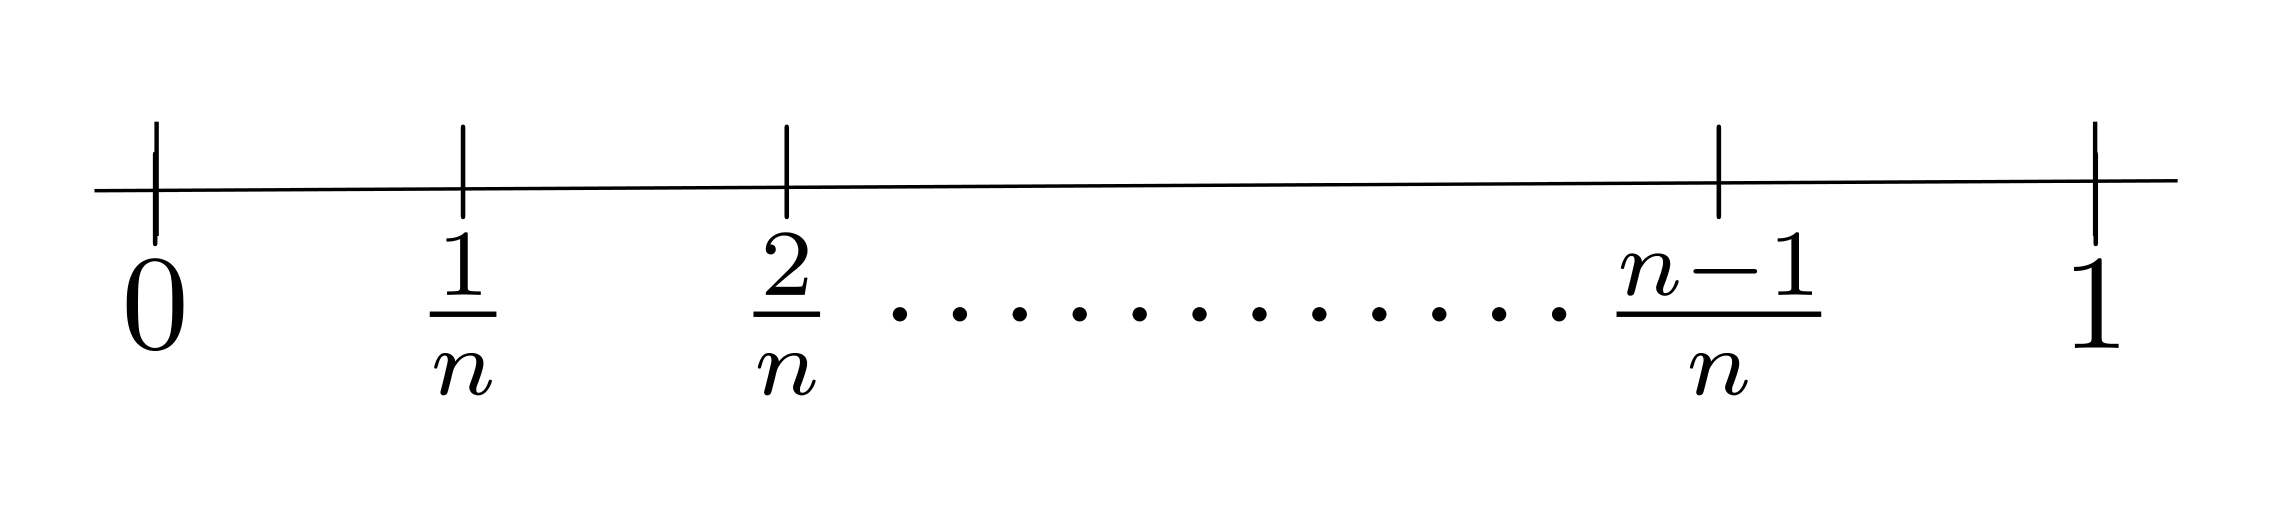
\includegraphics[width=0.6\textwidth]{142.png}
\end{center}

e considerar \ \ \ $\Gamma_{0},\Gamma_{1/n},\Gamma_{2/n},$ $\ldots$
$,\Gamma_{n-1/n},\Gamma_{1}.$ Se $n$ for suficientemente grande,

é claro que $k/n$ e $k+1/n$ serão próximos e então, pela
continuidade uniforme

de $H,$ podemos esperar que $\Gamma_{k/n}$ e $\Gamma_{k+1/n}$ são
"próximas" e que $\alpha\notin\Omega$ \"{e}stá

mais longe de $\Gamma_{k/n}$ e $\Gamma_{k+1/n}$ que estas entre si", donde
resultaria, aplicando

$n+2$ vezes o Lema 7.5, que

\bigskip

$(  (  \ast)  )  $ \ \ \ \ \ \ \ \ \ \ \textsc{I}%
nd$_{\Gamma_{0}}(  \alpha)  =$\textsc{I}nd$_{\Gamma_{1/n}}(
\alpha)  =$ $\ldots\ldots\ldots=$\textsc{I}nd$_{\Gamma_{n-1/n}}(
\alpha)  =$\textsc{I}nd$_{\Gamma_{1}}(  \alpha)  $

% IMAGEM 31

\begin{center}
  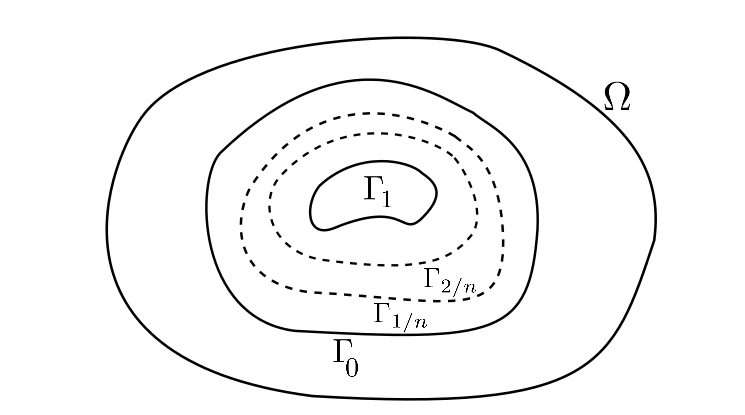
\includegraphics[width=0.55\textwidth]{31.png}
\end{center}

Entretanto, há uma objeção lógica à linha de
raciocínio precedente devida

ao seguinte fato: não há nada na definição de homotopia que
nos permita

assegurar que as curvas fechadas $\Gamma_{k/n}$ $(  k=0,1,\text{ }%
\ldots,n)  $ sejam \textit{CSDF}, e

então a expressão \textsc{I}nd$_{\Gamma_{k/n}}(  \alpha)  $
pode não estar definida. Como a forma mais

simples de obtermos uma \textit{CSDF} "próxima" de uma curva fechada
$\gamma$ dada,

é construir uma poligonal fechada de vértices em $\gamma,$ vamos
modificar o ra-

ciocínio descrito acima substituindo a sequência $\Gamma_{0}%
,\Gamma_{1/n},$ $\ldots$ $,\Gamma_{1}$ por uma

sequência de poligonais fechadas $\gamma_{0},\gamma_{1},$ $\ldots,$
$\gamma_{n},$ onde $\gamma_{k}$ tem seus vértices

em $\Gamma_{k/n}.$ No fim em vez de $(  (  \ast)  )  $ \ teremos

\ \ \ \ \ \ \ \ \ \textsc{I}nd$_{\Gamma_{0}}(  \alpha)
=$\textsc{I}nd$_{\gamma_{0}}(  \alpha)  =$\textsc{I}nd$_{\gamma
_{1}}(  \alpha)  =$ $\ldots\ldots=$\textsc{I}nd$_{\gamma_{n}%
}(  \alpha)  =$\textsc{I}nd$_{\Gamma_{1}}(  \alpha)  $

% IMAGEM 32

\begin{center}
  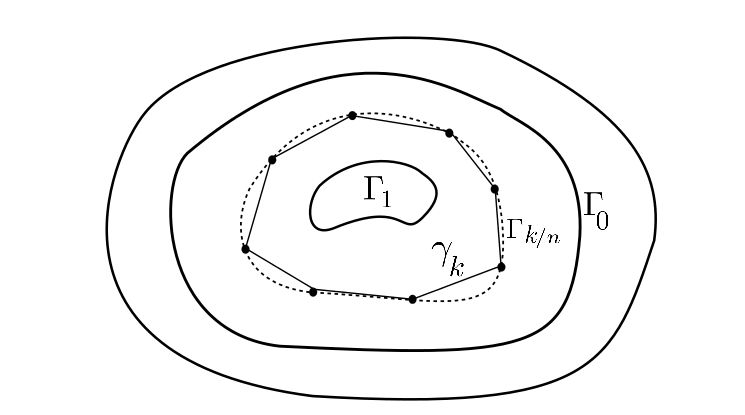
\includegraphics[width=0.6\textwidth]{32.png}
\end{center}

\textbf{Prova \ da Prop. 7.6 \ Se }$\Omega=%
%TCIMACRO{\U{2102} }%
%BeginExpansion
\mathbb{C}
%EndExpansion
$ então $(  7.1.1)  $ vale automáticamente, isto

é, $\Gamma_{0}-\Gamma_{1}\overset{%
%TCIMACRO{\U{2102} }%
%BeginExpansion
\mathbb{C}
%EndExpansion
}{\backsim}0$ donde $\Gamma_{0}\overset{%
%TCIMACRO{\U{2102} }%
%BeginExpansion
\mathbb{C}
%EndExpansion
}{\backsim}\Gamma_{1}$ o que mostra que o resultado é trivial neste

caso logo podemos supor $\Omega\neq%
%TCIMACRO{\U{2102} }%
%BeginExpansion
\mathbb{C}
%EndExpansion
.$ Fixemos $\alpha\notin\Omega.$ Suponhamos para

simplificar que $\Gamma_{0}$ e $\Gamma_{1}$ têm como domínio
\textsc{I} $=\left[  0,1\right]  ,$ então por definição

existe $H\in\mathcal{C}(  \text{\textsc{I}}^{2},\Omega)  $ tal que

\bigskip

$(  7.6.1)  $ \ \ \ $\ \ \left\vert
\begin{array}
[c]{c}%
H(  s,0)  =\Gamma_{0}(  s)  \ ,\ H(  s,1)
=\Gamma_{1}(  s)  \ e\ H(  0,t)  =H(  1,t)
\text{ \ \ \ \ \ \ }\\
\forall\ (  s,t)  \in\text{\textsc{I}}^{2}.\text{
\ \ \ \ \ \ \ \ \ \ \ \ \ \ \ \ \ \ \ \ \ \ \ \ \ \ \ \ \ \ \ \ \ \ \ \ \ \ \ \ \ \ \ \ \ \ \ \ \ \ \ \ \ \ \ \ \ \ \ \ \ \ \ }%
\end{array}
\right.
\ \ \ \ \ \ \ \ \ \ \ \ \ \ \ \ \ \ \ \ \ \ \ \ \ \ \ \ \ \ \ \ \ \ \ \ \ \ \ \ \ \ \ \ \ \ \ \ \ \ \ \ \ \ \ \ \ \ \ \ \ \ \ \ \ \ \ \ \ \ \ \ \ \ \ \ \ \ \ \ \ \ \ \ \ \ \ \ \ \ \ \ \ \ \ \ \ $
\ \ 

\bigskip

Como \textsc{I}$^{2}$ é compacto, $H(  \text{\textsc{I}}^{2})
$ também é compacto e como

\ \ \ \ \ \ \ \ \ \ \ \ \ dist$(  \alpha,H(  \text{\textsc{I}}%
^{2})  )  \geq dist(  \partial\Omega,H(
\text{\textsc{I}}^{2})  )  >0$

é claro que existe $\varepsilon>0$ tal que

\bigskip

$(  7.6.2)  $ \ \ \ \ \ \ \ \ \ \ \ \ \ \ \ \ \ \ \ \ $\left\vert
\alpha-H(  s,t)  \right\vert >2\varepsilon$ \ \ \ \ $\forall$
\ \ $(  s,t)  \in$ \textsc{I}$^{2}.$

\bigskip

Como $H$ é uniformemente contínua, existe $n\in%
%TCIMACRO{\U{2115} }%
%BeginExpansion
\mathbb{N}
%EndExpansion
^{\ast}$ tal que

\bigskip

$(  7.6.3)  $ \ \ \ \ \ $\left\vert s-s^{\prime}\right\vert
+\left\vert t-t^{\prime}\right\vert \leq\dfrac{1}{n}$ \ $\implies$
\ $\left\vert H(  s,t)  -H(  s^{\prime},t^{\prime})
\right\vert <\varepsilon$ $.$

\bigskip

Para cada $t\in$ \textsc{I,} seja $\Gamma_{t}:s\in$ \textsc{I }$\longmapsto
H(  s,t)  \in\Omega$ e consideremos as $n+1$

curvas fechadas $\Gamma_{0},\Gamma_{1/n},$ $\ldots$ $,\Gamma_{n-1/n}%
,\Gamma_{1}.$ Para cada $k=0,1,$ $\ldots,n$ vamos

construir uma poligonal $\gamma_{k}$ cujos vértices estão em
$\Gamma_{k}$ da maneira seguinte.

Dividimos \textsc{I} em $n$ intervalos iguais

\ \ \ \ \ \ \ \ \ \ \ \ \ \ \ \ \ \ \ \ \ \ \ \ \ \ \ \ \ \ \ \ \ $J_{i}%
=\left[  \dfrac{i-1}{n},\text{ }\dfrac{i}{n}\right]  $
\ \ \ \ \ \ \ \ \ \ $(  i=1,2,\ldots,n)  $

e para cada $k=0,1,$ $\ldots,n$ definimos $\gamma_{k}$ sobre $J_{i}$ por

\bigskip

$(  7.6.4)  $ \ \ $\left\vert
\begin{array}
[c]{c}%
\gamma_{k}(  s)  =H(  \dfrac{i}{n},\dfrac{k}{n})
(  ns+1-i)  +H(  \dfrac{i-1}{n},\dfrac{k}{n})  (
i-ns)  \ \\
\ \\
\ \forall\ s\in J_{i}=\left[  \dfrac{i-1}{n},\dfrac{i}{n}\right]  \text{
\ \ \ \ \ \ \ \ \ \ \ \ \ \ \ \ \ \ \ \ \ \ \ \ \ \ \ \ \ \ \ \ \ \ \ \ \ \ \ \ \ \ \ \ \ \ \ \ }%
\end{array}
\right.  \ \ \ \ \ $

$\bigskip$

(Observe que $\forall$ $\ s\in J_{i}\ \ $tem-se\ $\ i-1\leq ns\leq i\ \ $donde
$\ i-ns\geq0,$

$ns+1-i\geq0$ e $(  i-ns)  \ +(  ns+1-i)  =1$ o que
implica $\ \ \gamma_{k}(  s)  =$

$H(  \dfrac{i-1}{n},\dfrac{k}{n})  \lambda+\ H(  \dfrac{i}%
{n},\dfrac{k}{n})  (  1-\lambda)  \ ,$ com $\lambda
:=i-ns\ $\ e como a imagem

de $J_{i}\ $pela aplicação $s\longmapsto\lambda$ é $\left[
0,1\right]  $ $\ $é\ claro\ que\ $\ \ \ \ $

$\ \ \ \ \ \ \ \ \ \ \ \ \ \ \ \ \ \ \ \ (  \gamma_{k}|J_{i})
^{\ast}=\left[  H(  \dfrac{i-1}{n},\dfrac{k}{n})  ,H(
\dfrac{i}{n},\dfrac{k}{n})  \right]  \ $).

% IMAGEM 33

\begin{center}
  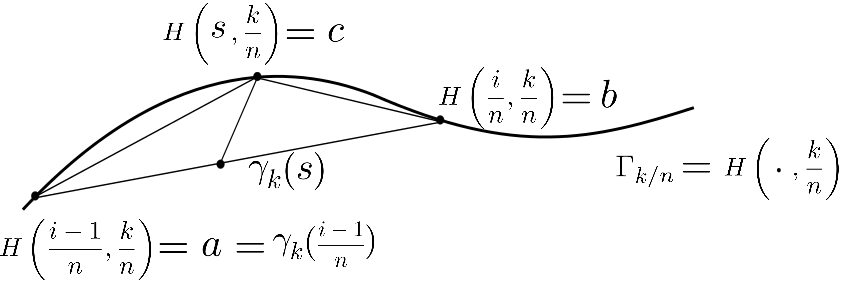
\includegraphics[width=0.7\textwidth]{33.png}
\end{center}

Mostremos a seguir que de $(  7.6.3)  $ e de $(  7.6.4)  $ resulta

\bigskip

$(  7.6.5)  $ \ \ \ \ \ $\left\vert \gamma_{k}(  s)
-H(  s,k/n)  \right\vert <\varepsilon$ \ \ \ \ $\forall$
\ \ $k=0,1,$ $\ldots,n$ \ \ e \ \ $\forall$ \ \ $s\in$ \textsc{I}

\bigskip

De fato, por $(  7.6.3)  $ resulta que os lados do tri\^{a}ngulo
$(  a,b,c)  $ na figura

anterior têm comprimento $<\varepsilon$ \ e como di\^{a}metro de um
\ tri\^{a}ngulo é o

comprimento do maior dos seus lados, é claro que temos $(
7.6.5)  .$

Como $(  7.6.5)  $ se escreve

\ \ \ \ \ \ \ \ \ \ \ \ \ $\left\vert \gamma_{k}(  s)
-\Gamma_{k/n}(  s)  \right\vert <\varepsilon$ \ \ \ \ $\forall$
\ \ $k=0,1,$ $\ldots,n$ \ \ e \ \ $\forall$ \ \ $s\in$ \textsc{I}

resulta em particular para $k=0$ e $k=n:$

\bigskip

$(  7.6.6)  $ \ \ \ \ \ \ \ $\left\vert \gamma_{0}(  s)
-\Gamma_{0}(  s)  \right\vert <\varepsilon$ \ \ \ \ e
\ \ \ \ \ $\left\vert \gamma_{n}(  s)  -\Gamma_{1}(  s)
\right\vert <\varepsilon$ \ \ \ \ $\forall$ \ \ $s\in$ \textsc{I}

\bigskip

De $(  7.6.2)  ,(  7.6.5)  $ e da propriedade triangular resulta:

\ \ \ \ \ \ \ \ \ \ \ \ \ \ $\left\vert \alpha-\gamma_{k}(  s)
\right\vert \geq\left\vert \alpha-H(  s,k/n)  \right\vert
-\left\vert H(  s,k/n)  -\gamma_{k}(  s)  \right\vert
>\varepsilon,$ \ portanto

\bigskip

$(  7.6.7)  $ \ \ \ \ \ \ $\left\vert \alpha-\gamma_{k}(
s)  \right\vert >\varepsilon$ \ \ \ \ $\forall$ \ \ $k=0,1,$ $\ldots,n$
\ \ e \ \ $\forall$ \ $s\in$ \textsc{I}

\bigskip

Por outro lado (fazendo as contas), de $(  7.6.3)  $ e $(
7.6.4)  $ segue

\bigskip

$(  7.6.8)  $ \ \ \ \ \ $\left\vert \gamma_{k-1}(  s)
-\gamma_{k}(  s)  \right\vert <\varepsilon$ \ \ \ \ $\forall$
\ \ $k=0,1,$ $\ldots,n$ \ \ e \ \ $\forall$ \ \ $s\in$ \textsc{I}

\bigskip

Finalmente, de $(  7.6.6)  ,(  7.6.7)  $ \ e \ $(
7.6.8)  $ e aplicando $n+2$ vezes o Lema

7.5 obtemos \textsc{I}nd$_{\Gamma_{0}}(  \alpha)  =$ \textsc{I}%
nd$_{\gamma_{0}}(  \alpha)  =$ $\ldots$ $=$ \textsc{I}%
nd$_{\gamma_{n}}(  \alpha)  =$ \textsc{I}nd$_{\Gamma_{1}}(
\alpha)  ,$ o que

prova que $\Gamma_{0}\overset{\Omega}{\backsim}\Gamma_{1}.$ Dizer que $\Gamma$
é homotopica a um ponto $\zeta\in\Omega$ \ signifi-

ca por definição que $\Gamma$ é homotópica a uma curva constante

$\widetilde{\Gamma}:t\in$ \textsc{I} $\longmapsto\zeta\in\Omega.$ Pelo que
precede temos \textsc{I}nd$_{\Gamma}(  \alpha)  =$ \textsc{I}%
nd$_{\widetilde{\Gamma}}(  \alpha)  $ \ $\forall$ \ $\alpha
\notin\Omega$ \ 

e visivelmente \textsc{I}nd$_{\widetilde{\Gamma}}(  \alpha)  =0$
\ \ \ $\forall$ \ \ $\alpha\neq\zeta.$ $\square$

\bigskip

A recíproca da Prop. 7.6 é falsa, ver exerc. (7.4).

\bigskip

O resultado seguinte é a "versão homotópica" do teorema de Cauchy
e é

de fato a mais utilizada nas aplicações.

\bigskip

\textbf{Teorema 7.7 \ }(Cauchy) \ \textit{Sejam }$\Omega$ \textit{um aberto
não vazio arbitrário de }$%
%TCIMACRO{\U{2102} }%
%BeginExpansion
\mathbb{C}
%EndExpansion
$

\textit{e }$f\in\mathcal{H}(  \Omega)  .$ \textit{Então:}

(1%
%TCIMACRO{\U{ba}}%
%BeginExpansion
${{}^o}$%
%EndExpansion
) \ \textit{Se }$\gamma$ \textit{é uma CSDF em }$\Omega$ \textit{e
}$\gamma$ \textit{é homotópica a um ponto em }$\Omega,$
\textit{então}

\bigskip

\ \ \ \ \ \ \ \ \ \ \ \ $f(  z)  .$\textsc{I}nd$_{\gamma}(
z)  =\dfrac{1}{2\pi i}\underset{\gamma}{%
%TCIMACRO{\dint }%
%BeginExpansion
{\displaystyle\int}
%EndExpansion
}\dfrac{f(  w)  dw}{w-z}$ \ \ \ \ \ $\forall$ \ \ \ $z\in
\Omega\backslash\gamma^{\ast}$

\textit{e}

\ \ \ \ \ \ \ \ \ \ \ \ \ \ \ \ \ \ \ \ \ \ \ \ \ \ \ \ \ $\underset{\gamma}{%
%TCIMACRO{\dint }%
%BeginExpansion
{\displaystyle\int}
%EndExpansion
}f(  z)  dz=0$ $.$

\bigskip

(2%
%TCIMACRO{\U{ba}}%
%BeginExpansion
${{}^o}$%
%EndExpansion
) \ \textit{Se }$\gamma_{1}$ \textit{e }$\gamma_{2}$ \textit{são duas CSDF
em }$\Omega$ \textit{e }$\gamma_{1}$ \textit{e }$\gamma_{2}$ \textit{são
}$\Omega$\textit{-HCF, então}

\bigskip

\ \ \ \ \ \ \ \ \ \ \ \ \ \ \ \ \ \ \ \ \ \ \ $\underset{\gamma_{1}}{%
%TCIMACRO{\dint }%
%BeginExpansion
{\displaystyle\int}
%EndExpansion
}f(  z)  dz=\underset{\gamma_{2}}{%
%TCIMACRO{\dint }%
%BeginExpansion
{\displaystyle\int}
%EndExpansion
}f(  z)  dz$ $.$

\bigskip

\textbf{Prova \ }(1%
%TCIMACRO{\U{ba}}%
%BeginExpansion
${{}^o}$%
%EndExpansion
) \ Se $\gamma$ é homotópica a um ponto em $\Omega,$ a última
asserção da

Prop.7.6 mostra que $\gamma\overset{\Omega}{\backsim}0$ e, em
consequência, o resultado é um caso

particular do Teor. 7.1 (1%
%TCIMACRO{\U{ba}}%
%BeginExpansion
${{}^o}$%
%EndExpansion
).

(2%
%TCIMACRO{\U{ba}}%
%BeginExpansion
${{}^o}$%
%EndExpansion
) \ Se $\gamma_{1\text{ }}$e $\gamma_{2}$ são $\Omega$-\textit{HCF}, pela
primeira parte da Prop. 7.6 resulta que

$\gamma_{1}\overset{\Omega}{\backsim}\gamma_{2},$ logo o resultado é um
caso particular do Teor. 7.1 (2%
%TCIMACRO{\U{ba}}%
%BeginExpansion
${{}^o}$%
%EndExpansion
) . $\square$

\bigskip

Uma outra forma muito utilizada do teorema de Cauchy é a seguinte em que

$\Omega$ é suposto simplesmente conexo:

\bigskip

\textbf{Teorema 7.8 }\ \textit{Seja }$\Omega$ \textit{\ um aberto simplesmente
conexo de }$%
%TCIMACRO{\U{2102} }%
%BeginExpansion
\mathbb{C}
%EndExpansion
$ \textit{e }$f\in\mathcal{H}(  \Omega)  .$

\textit{Se }$\gamma$ \textit{é uma CSDF em }$\Omega,$ \textit{então:}

\bigskip

\ \ \ \ \ \ \ \ \ \ \ \ \ $f(  z)  $\textsc{I}nd$_{\gamma}(
z)  dz=\dfrac{1}{2\pi i}\underset{\gamma}{%
%TCIMACRO{\dint }%
%BeginExpansion
{\displaystyle\int}
%EndExpansion
}\dfrac{f(  w)  dw}{w-z}$ \ \ \ \ $\forall$ \ \ \ $z\in
\Omega\backslash\gamma^{\ast}$

\textit{e}

\ \ \ \ \ \ \ \ \ \ \ \ $\underset{\gamma}{%
%TCIMACRO{\dint }%
%BeginExpansion
{\displaystyle\int}
%EndExpansion
}f(  z)  dz=0$ .

\bigskip

\textbf{Prova \ }Como\textbf{\ }$\Omega$ é simplesmente conexo e $\gamma$
é uma \textit{CSDF} em $\Omega,$ é claro que

$\gamma$ é homotópica a um ponto em $\Omega$ e portanto o resultado
é um caso particular

do Teor. 7.7 (1%
%TCIMACRO{\U{ba}}%
%BeginExpansion
${{}^o}$%
%EndExpansion
). $\square$

\bigskip

\textbf{Observação \ }Nas hipóteses do Teor. 7.8, a
asserção correspondente a (2%
%TCIMACRO{\U{ba}}%
%BeginExpansion
${{}^o}$%
%EndExpansion
)

do Teor. 7.7, isto é, "Se $\Omega$ é simplesmente conexo,
$f\in\mathcal{H}(  \Omega)  $\ e $\gamma_{1}$\ \ e $\gamma_{2}$\ são



duas\ \textit{CSDF} em $\Omega$ então $\underset{\gamma_{1}}{%
%TCIMACRO{\dint }%
%BeginExpansion
{\displaystyle\int}
%EndExpansion
}f=\underset{\gamma2}{%
%TCIMACRO{\dint }%
%BeginExpansion
{\displaystyle\int}
%EndExpansion
}f$ \ ", é verdadeira porém absolutamente

trivial pois ambas\ \ integrais são nulas (pelo Teor. 7.8). Esta é a
razão pela



qual enunciamos o Teor. 7.8 sem a parte (2%
%TCIMACRO{\U{ba}}%
%BeginExpansion
${{}^o}$%
%EndExpansion
).\ \ \ 



\bigskip

\textbf{Teorema 7.9 \ }(independência do caminho) \ \textit{Sejam }$\Omega$
\textit{um aberto não vazio} 

% IMAGEM 35

\begin{wrapfigure}{r}{0.25\textwidth}
  \begin{center}
    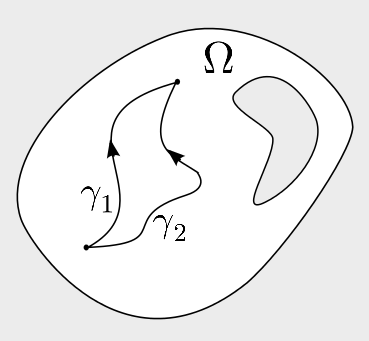
\includegraphics[width=0.25\textwidth]{35.png}
  \end{center}
\end{wrapfigure}

de
$%
%TCIMACRO{\U{2102} }%
%BeginExpansion
\mathbb{C}
%EndExpansion
,$ \textsc{I} \textit{um intervalo compacto e }$\gamma_{1}:$\ \textsc{I}
$\rightarrow\Omega$ ,

\ $\gamma_{2}:$ \textsc{I} $\rightarrow\Omega$
\ \textit{duas CSD em }$\Omega$ \textit{com mesma origem e}

 mesmo extremo.

(1%
%TCIMACRO{\U{ba}}%
%BeginExpansion
${{}^o}$%
%EndExpansion
) \ \textit{Se }$\gamma_{1}$ \textit{e }$\gamma_{2}$ \textit{são }$\Omega
$-\textit{HEF, então}

\ \ \ \ \ \ \ \ \ \ \ \ \ \ \ \ \ \ \ \ \ \ \ \ \ \ \ \ $\underset{\gamma_{1}%
}{%
%TCIMACRO{\dint }%
%BeginExpansion
{\displaystyle\int}
%EndExpansion
}f=\underset{\gamma_{2}}{%
%TCIMACRO{\dint }%
%BeginExpansion
{\displaystyle\int}
%EndExpansion
}f$ \ \ \ \ $\forall$ \ \ $f\in\mathcal{H}(  \Omega)  .$

\bigskip

(2%
%TCIMACRO{\U{ba}}%
%BeginExpansion
${{}^o}$%
%EndExpansion
) \ \textit{Se }$\Omega$ \textit{é simplesmente conexo, então}

\ \ \ \ \ \ \ \ \ \ \ \ \ \ \ \ \ \ \ \ \ \ \ \ \ \ \ \ $\underset{\gamma_{1}%
}{%
%TCIMACRO{\dint }%
%BeginExpansion
{\displaystyle\int}
%EndExpansion
}f=\underset{\gamma_{2}}{%
%TCIMACRO{\dint }%
%BeginExpansion
{\displaystyle\int}
%EndExpansion
}f$ \ \ \ \ \ $\forall$ \ \ $f\in\mathcal{H}(  \Omega)  .$

\bigskip

\textbf{Prova \ }(1%
%TCIMACRO{\U{ba}}%
%BeginExpansion
${{}^o}$%
%EndExpansion
) \ Pelo exerc. (7.2) sabemos que $\gamma_{1}\vee\gamma_{2}^{0}$ é 

uma CSDF em $\Omega$ homotópica a um ponto em $\Omega$ e 

então, pelo Teor. 7.7 (1${{}^o}$) resulta para $f\in\mathcal{H}(  \Omega)  $ ar-

bitária:

\bigskip

$(  7.9.1)  $ \ \ \ \ \ \ $0=\underset{\gamma_{1}\vee\gamma_{2}%
^{0}}{%
%TCIMACRO{\dint }%
%BeginExpansion
{\displaystyle\int}
%EndExpansion
}f=\underset{\gamma_{1}}{%
%TCIMACRO{\dint }%
%BeginExpansion
{\displaystyle\int}
%EndExpansion
}f+\underset{\gamma_{2}^{o}}{%
%TCIMACRO{\dint }%
%BeginExpansion
{\displaystyle\int}
%EndExpansion
}f=\underset{\gamma_{1}}{%
%TCIMACRO{\dint }%
%BeginExpansion
{\displaystyle\int}
%EndExpansion
}f-\underset{\gamma_{2}}{%
%TCIMACRO{\dint }%
%BeginExpansion
{\displaystyle\int}
%EndExpansion
}f$ \ \ $,$

\bigskip

o que prova a asserção.

(2%
%TCIMACRO{\U{ba}}%
%BeginExpansion
${{}^o}$%
%EndExpansion
) \ É claro que $\gamma_{1}\vee\gamma_{2}^{0}$ \ é uma \textit{CSDF}
em $\Omega$ e como $\Omega$ é simplesmente

conexo, pelo Teor. 7.8 (1%
%TCIMACRO{\U{ba}}%
%BeginExpansion
${{}^o}$%
%EndExpansion
), podemos escrever (7.9.1), o que prova a

asserção neste caso. $\square$

\bigskip

Se $\Omega$ é um aberto \textit{simplesmente conexo, }$z,w\in\Omega$
são pontos arbitrários, $\gamma$

é uma \textit{CSD} em $\Omega$ de origem $z$ e extremo $w$ e
$f\in\mathcal{H}(  \Omega)  ,$ pelo Teor. 7.9 (2%
%TCIMACRO{\U{ba}}%
%BeginExpansion
${{}^o}$%
%EndExpansion
),

o valor da integral

\ \ \ \ \ \ \ \ \ \ \ \ \ \ \ \ \ \ \ \ \ \ \ \ \ \ \ \ \ \ \ \ \ \ \ \ \ \ \ \ $\underset
{\gamma}{%
%TCIMACRO{\dint }%
%BeginExpansion
{\displaystyle\int}
%EndExpansion
}f$

depende apenas dos pontos $z$ e $w$ e não da particular \textit{CSD}
$\gamma$ em $\Omega$ de origem

$z$ e extremo $w.$ No que segue indicaremos o valor comum de todas estas inte-

grais pela notação

\ \ \ \ \ \ \ \ \ \ \ \ \ \ \ \ \ \ \ \ \ \ \ \ \ \ \ \ \ \ \ \ \ \ \ \ \ \ $\underset
{z}{%
%TCIMACRO{\dint }%
%BeginExpansion
{\displaystyle\int}
%EndExpansion
}^{w}f=\underset{z}{%
%TCIMACRO{\dint }%
%BeginExpansion
{\displaystyle\int}
%EndExpansion
}^{w}f(  \lambda)  d\lambda$ $.$



\bigskip

\textbf{Corolário 7.10 \ }\textit{Se }$\Omega$ \textit{é um aberto
simplesmente conexo de }$%
%TCIMACRO{\U{2102} }%
%BeginExpansion
\mathbb{C}
%EndExpansion
$ \textit{e }$f\in\mathcal{H}(  \Omega)  ,$

% IMAGEM 36


\textit{então }$f$ \textit{possui uma primitiva em }$\Omega.$

\bigskip

\textbf{Prova \ }Fixemos $a\in\Omega$ arbitrário, então pelo Teor. 7.9(2${{}^o}$%
%EndExpansion
), fica definida 

uma função

\bigskip

\begin{wrapfigure}{r}{0.35\textwidth}
  \begin{center}
    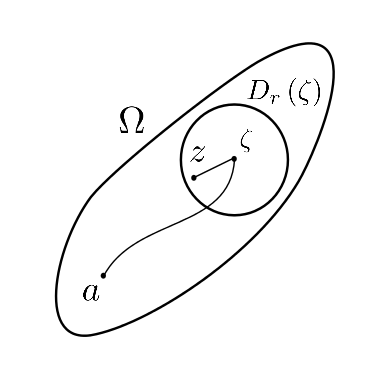
\includegraphics[width=0.35\textwidth]{36.png}
  \end{center}
\end{wrapfigure}


\ \ \ \ \ \ \ \ \ \ \ \ \ \ \ \ \ \ \ \ \ \ \ \ \ $F:z\in
\Omega\longmapsto\underset{a}{%
%TCIMACRO{\dint }%
%BeginExpansion
{\displaystyle\int}
%EndExpansion
}^{z}f$ \ \ \ $\in$ \ $%
%TCIMACRO{\U{2102} }%
%BeginExpansion
\mathbb{C}
%EndExpansion
,$

mostremos que

\bigskip
\ \ \ \ \ \ \ \ \ \ \ \ \ \ \ \ $F^{\prime}(
z)  =f(  z)  $ \ \ \ \ \ $\forall$ \ \ \ $z\in\Omega$ $.$

\bigskip

Fixados $\zeta\in\Omega$ e $D_{r}(  \zeta)  \subset\Omega,$ \ se
\ $z\in D_{r}(  \zeta)  $ \ 

temos

\bigskip

\ \ \ \ \ \ \ \ \ $F(  z)  =\underset{a}{%
%TCIMACRO{\dint }%
%BeginExpansion
{\displaystyle\int}
%EndExpansion
}^{z}f=\underset{z}{%
%TCIMACRO{\dint }%
%BeginExpansion
{\displaystyle\int}
%EndExpansion
}^{\zeta}f+\underset{\left[  \zeta,z\right]  }{%
%TCIMACRO{\dint }%
%BeginExpansion
{\displaystyle\int}
%EndExpansion
}f=$

\ \ \ \ \ \ \ \ \ 	$F(  \zeta)  +\underset{\left[  \zeta,z\right]  }{%
%TCIMACRO{\dint }%
%BeginExpansion
{\displaystyle\int}
%EndExpansion
}f(  \lambda)  d\lambda$

donde

\bigskip

\ \ \ \ \ \ \ \ \ \ \ \ \ \ \ \ \ \ \ \ \ \ $\dfrac{F(  z)  -F(
\zeta)  }{z-\zeta}=\dfrac{1}{z-\zeta}\underset{\left[  \zeta,z\right]
}{%
%TCIMACRO{\dint }%
%BeginExpansion
{\displaystyle\int}
%EndExpansion
}f(  \lambda)  d\lambda$

o que implica

\bigskip

$$\text{\ \ \ \ \ \ \ \ \ \ \ \ \ \ \ \ \ \ }\dfrac{F(  z)  -F(
\zeta)  }{z-\zeta}-f(  \zeta)  =\dfrac{1}{z-\zeta}%
\underset{\left[  \zeta,z\right]  }{%
%TCIMACRO{\dint }%
%BeginExpansion
{\displaystyle\int}
%EndExpansion
}\left[  f(  \lambda)  -f(  \zeta)  \right]  d\lambda$$

e em consequência:

\bigskip

$$\left\vert \dfrac{F(  z)
-F(  \zeta)  }{z-\zeta}-f(  \zeta)  \right\vert
\leq\underset{\lambda\in\left[  \zeta,z\right]  ^{\ast}}{\sup}\left\vert
f(  \lambda)  -f(  \zeta)  \right\vert 
\text{\ \ \ \ } \forall \text{\ \ } z\in D_{r}(  \zeta)  $$

\bigskip

o que mostra pela continuidade de $f$ em $\zeta:$

\bigskip

\ \ \ \ \ \ \ \ \ \ \ \ \ \ \ \ \ \ \ \ \ \ \ $\underset{z\rightarrow\zeta
}{\lim}\dfrac{F(  z)  -F(  \zeta)  }{z-\zeta}=f(
\zeta)  $ $.$ $\square$

\bigskip

Como consequência do Corol. 7.10 resulta que se $\Omega$ é um aberto simples-

mente conexo, \ $f\in\mathcal{H}(  \Omega)  $ e $f(  z)
\neq0$ para cada $z\in\Omega,$ então podemos

definir em $\Omega$ um ramo do logaritmo de $f$ (comparar a
demonstração do

próximo resultado com a do Teor. 6.4).

\bigskip

\textbf{Corolário 7.11 \ }\textit{Sejam }$\Omega$ \textit{um aberto
simplesmente conexo e }$f\in\mathcal{H}(  \Omega)  $

\textit{tal que }$f(  z)  \neq0$ \textit{para cada }$z\in\Omega.$
\textit{Então existe }$g\in\mathcal{H}(  \Omega)  $ \textit{tal
que }

$f=\exp(  g)  .$ \textit{Se }$z_{0}\in\Omega$ \textit{e }$e^{w_{0}%
}=f(  z_{0})  ,$ \textit{a função }$g$ \textit{tal que
}$f=\exp(  g)  $ \textit{pode}

\textit{ser escolhida de modo a verificar a condição suplementar
}$g(  z_{0})  =w_{0}.$

\bigskip

\textbf{Prova \ }Por hipótese temos $f^{\prime}/f\in\mathcal{H}(
\Omega)  $ e como $\Omega$ é simplesmente conexo,

o Corol. 7.10 implica que $f^{\prime}/f$ possui uma primitiva $g_{1}%
\in\mathcal{H}(  \Omega)  .$ Se $h:=$

$\exp(  g_{1})  ,$ então $h\in\mathcal{H}(  \Omega)
$ e $h(  z)  \neq0$ para cada $z\in\Omega,$ donde $f/h\in
\mathcal{H}(  \Omega)  $

e

\ \ \ \ \ \ \ \ \ \ \ \ \ \ \ \ \ \ \ \ \ $(  f/h)  ^{\prime
}=\dfrac{f^{\prime}h-fh^{\prime}}{h^{2}}$ $.$

\bigskip

Por definição de $h$ e de $g_{1}$ temos

$\ \ \ \ \ \ \ \ \ \ \ \ \ \ \ $

$\ \ \ \ \ \ \ \ \ \ \ \ \ \ \ \ \ \ \ \ \ \ \ \ \ \ h^{\prime}=g_{1}^{\prime
}h=(  f^{\prime}/f)  h\implies f^{\prime}h-fh^{\prime}%
=0\implies(  f/h)  ^{\prime}=0$

e portanto $f/h$ é constante, isto é existe $c\in%
%TCIMACRO{\U{2102} }%
%BeginExpansion
\mathbb{C}
%EndExpansion
$ tal que

\bigskip

$(  7.11.1)  $ \ \ \ \ \ \ \ \ \ \ \ \ \ \ \ \ \ \ \ \ $\dfrac
{f(  z)  }{h(  z)  }=c$ \ \ \ \ \ \ \ $\forall$
\ \ \ $z\in\Omega$

\bigskip

Como $f(  z)  .h(  z)  \neq0$ para cada $z\in\Omega,$
é claro que $c\neq0,$ portanto existe

$c^{\prime}\in%
%TCIMACRO{\U{2102} }%
%BeginExpansion
\mathbb{C}
%EndExpansion
$ tal que $c=\exp(  c^{\prime})  $ e então, da
definição de $h$ e de $(  7.11.1)  $ resulta

\bigskip

$(  7.11.2)  $ \ \ \ \ \ \ \ \ \ \ \ \ \ \ \ \ \ \ $f=\exp(
g_{1}+c^{\prime})  $ $.$

\bigskip

Se $z_{0}\in\Omega$ \ e $w_{0}\in%
%TCIMACRO{\U{2102} }%
%BeginExpansion
\mathbb{C}
%EndExpansion
$ são tais que $e^{w_{0}}=f(  z_{0})  ,$ então por $(
7.11.2)  $ resulta

\ \ \ \ \ \ \ \ \ \ $e^{w_{0}}=\exp\left[  g_{1}(  z_{0})
+c^{\prime}\right]  \implies\exp\left[  w_{0}-g_{1}(  z_{0})
-c^{\prime}\right]  =1$

donde

\ \ \ \ \ \ \ \ \ \ \ \ \ \ \ \ \ \ \ \ \ \ \ \ \ $\dfrac{w_{0}-g_{1}(
z_{0})  -c^{\prime}}{2\pi i}=k\in%
%TCIMACRO{\U{2124} }%
%BeginExpansion
\mathbb{Z}
%EndExpansion
$

o que implica $w_{0}=g_{1}(  z_{0})  +c^{\prime}+2k\pi i$ \ e
então, definindo $g$ por

\ \ \ \ \ \ \ \ \ \ \ \ \ \ \ \ \ \ \ \ \ \ \ \ $g:=g_{1}+c^{\prime}+2k\pi i,$

é claro que $g(  z_{0})  =w_{0}$ e de $(  7.11.2)  $
resulta $f=\exp(  g)  .$ $\square$

\bigskip

O resultado seguinte dá a expressão integral do logaritmo complexo

análoga ao caso real.

\bigskip

\textbf{Proposição 7.12 \ }\textit{Seja }$D_{0}=\left\{  z\in%
%TCIMACRO{\U{2102} }%
%BeginExpansion
\mathbb{C}
%EndExpansion
\text{ }|\text{ }z\neq-\left\vert z\right\vert \right\}  .$ \textit{Fixados
}$k\in%
%TCIMACRO{\U{2124} }%
%BeginExpansion
\mathbb{Z}
%EndExpansion
$ \textit{\ e}

$w_{0}\in D_{0}$ \textit{arbitrários temos}

\bigskip

$Log_{k}(  w)  =Log_{k}(  w_{0})  +\underset{w_{0}}{%
%TCIMACRO{\dint ^{w}}%
%BeginExpansion
{\displaystyle\int^{w}}
%EndExpansion
}\dfrac{d\lambda}{\lambda}=\ln\left\vert w_{0}\right\vert +i(  Am(
w_{0})  +2k\pi)  +\underset{w_{0}}{%
%TCIMACRO{\dint }%
%BeginExpansion
{\displaystyle\int}
%EndExpansion
}^{w}\dfrac{d\lambda}{\lambda}$ $,$

\textit{para cada }$w\in D_{0}.$ \textit{Em particular }$(  \text{tomando
}k=0\text{ e }w_{0}=1)  $ \textit{temos:}

\bigskip

\ \ \ \ \ \ \ \ \ \ \ \ \ \ \ \ \ \ \ \ \ $Log(  w)  =\underset{1}{%
%TCIMACRO{\dint }%
%BeginExpansion
{\displaystyle\int}
%EndExpansion
}^{w}\dfrac{d\lambda}{\lambda}$ \ $,$ \ \textit{para cada} \ $w\in D_{0}$ $.$

(lembrar que $Log:=Log_{0}$)

\bigskip

\textbf{Prova \ }Seja\textbf{\ }$\varphi_{0}:z\in D_{0}\longmapsto1/z\in%
%TCIMACRO{\U{2102} }%
%BeginExpansion
\mathbb{C}
%EndExpansion
,$ então como $D_{0\text{ }}$ é simplesmente

conexo (por exemplo porque $D_{0}$ é $1$-estrelado, ver Exemplo que segue

à Def. 7.4\ \ \ e $\varphi_{0}\in\mathcal{H}(  D_{0})  ,$ a
prova do Corol. 7.10 mostra a função

\ \ \ \ \ \ \ \ \ \ \ \ \ \ \ \ \ \ \ 

\ \ \ \ \ \ \ \ \ \ \ \ \ \ \ \ \ \ \ \ \ $\Phi:w\in D_{0}\longmapsto
\underset{w_{0}}{%
%TCIMACRO{\dint }%
%BeginExpansion
{\displaystyle\int}
%EndExpansion
}^{w}\varphi_{0}(  \lambda)  d\lambda=\underset{w_{0}}{%
%TCIMACRO{\dint }%
%BeginExpansion
{\displaystyle\int}
%EndExpansion
}^{w}\dfrac{d\lambda}{\lambda}\in%
%TCIMACRO{\U{2102} }%
%BeginExpansion
\mathbb{C}
%EndExpansion
$

\bigskip

é uma primitiva de $\varphi_{0}$ em $D_{0},$ isto é, $\Phi^{\prime
}=\varphi_{0}$ em $D_{0}.$ Como $Log_{k}^{\prime}=\varphi_{0}$ em

$D_{0}$ (ver $\left[  5^{\prime}\right]  $\ pouco depois da Def. 6.12\ e a
definição de $Log_{k}$ logo após a

prova da Prop. 6.15), resulta que

\bigskip

\ \ \ \ \ \ \ \ \ \ $(  Log_{k}-\Phi)  ^{\prime}=Log_{k}^{\prime
}-\Phi^{\prime}=\varphi_{0}-\varphi_{0}=0$ \ \ \ em \ $D_{0}$

\bigskip

o que implica (por ser $D_{0}$ conexo e pelo Corol. 2.8) que $Log_{k}-\Phi$
é constante

em $D_{0},$ isto é, existe $c\in%
%TCIMACRO{\U{2102} }%
%BeginExpansion
\mathbb{C}
%EndExpansion
$ tal que

\bigskip

\ \ \ \ \ \ \ \ \ \ \ \ \ \ \ \ \ \ \ \ \ \ \ \ \ $Log_{k}(  w)
-\Phi(  w)  =c$ \ \ \ \ $\forall$ \ \ $w\in D_{0}$

isto é

\ \ \ \ \ \ \ \ \ \ \ \ \ \ \ \ \ \ \ \ \ \ \ \ \ $Log_{k}(  w)
=c+\underset{w_{0}}{%
%TCIMACRO{\dint }%
%BeginExpansion
{\displaystyle\int}
%EndExpansion
}^{w}\dfrac{d\lambda}{\lambda}$ \ \ \ \ $\forall$ \ \ $w\in D_{0}$

\bigskip

o que para $w=w_{0}$ implica \ $c=Log_{k}(  w_{0})  .$ $\square$

\bigskip

Encerramos este capítulo com uma fórmula de representação
integral para

as derivadas sucessivas de uma função analítica que generaliza fortemente

o Corol. 5.10. Precisaremos do seguinte:

\bigskip

\textbf{Lema 7.13} \ \textit{Seja }$\gamma$\textit{\ uma CSD em }$%
%TCIMACRO{\U{2102} }%
%BeginExpansion
\mathbb{C}
%EndExpansion
$\textit{\ e seja }$\varphi\in\mathcal{C}(  \gamma^{\ast})  .$ Para
cada $m\in%
%TCIMACRO{\U{2115} }%
%BeginExpansion
\mathbb{N}
%EndExpansion
,$

$m\geq1$\textit{\ consideremos a função}

\bigskip\ \ \ \ \ \ \ \ \ \ \ \ \ \ \ \ \ \ \ \ \ \ $F_{m}:z\in\complement
\gamma^{\ast}\longmapsto\underset{\gamma}{%
%TCIMACRO{\dint }%
%BeginExpansion
{\displaystyle\int}
%EndExpansion
}\dfrac{\varphi(  \lambda)  d\lambda}{(  \lambda-z)
^{m}}\in%
%TCIMACRO{\U{2102} }%
%BeginExpansion
\mathbb{C}
%EndExpansion
$ $.$

\textit{Então }$F_{m}\in\mathcal{H}(  \complement\gamma^{\ast
})  $ \textit{e }$F_{m}^{\prime}(  z)  =mF_{m+1}(
z)  $ \ \ \ \ $\forall$ \ \ $z\in\complement\gamma^{\ast}.$

\bigskip

\textbf{Prova \ }Começamos provando que $F_{1}$ é contínua. Sejam
$a\in\complement\gamma^{\ast}$ arbitrário

e $\delta>0$ tal que $D_{\delta}(  a)  \cap\gamma^{\ast
}=\varnothing.$ É claro que para cada $z\in D_{\delta/2}(  a)
$ temos

$\left\vert \lambda-z\right\vert >\delta/2$ para cada $\lambda\in\gamma^{\ast
},$ o que implica

\bigskip

$(  7.13.1)  $ \ \ \ \ \ \ \ $\dfrac{1}{\left\vert \lambda
-z\right\vert \left\vert \lambda-a\right\vert }\leq\dfrac{1}{(
\delta/2)  \delta}=\dfrac{2}{\delta^{2}}$ \ \ \ \ $\forall$
\ \ \ $\left\{
\begin{array}
[c]{c}%
\lambda\in\gamma^{\ast}\text{ \ \ \ \ \ \ \ }\\
z\in D_{\delta/2}(  a)
\end{array}
\right.  $

\bigskip

Ora, a definição de $F_{1}$ mostra que

\bigskip

$(  7.13.2)  $ \ \ \ \ \ \ \ \ \ \ \ \ \ \ \ \ $F_{1}(
z)  -F_{1}(  a)  =(  z-a)  \underset{\gamma}{%
%TCIMACRO{\dint }%
%BeginExpansion
{\displaystyle\int}
%EndExpansion
}\dfrac{\varphi(  \lambda)  d\lambda}{(  \lambda-z)
(  \lambda-a)  }$

\bigskip

o que junto a $(  7.13.1)  $ \ acarreta

\bigskip

\ \ \ \ \ \ \ $\left\vert F_{1}(  z)  -F_{1}(  a)
\right\vert \leq\left\vert z-a\right\vert \dfrac{2}{\delta^{2}}\underset
{\gamma}{%
%TCIMACRO{\dint }%
%BeginExpansion
{\displaystyle\int}
%EndExpansion
}\left\vert \varphi(  \lambda)  \right\vert \left\vert
d\lambda\right\vert $ \ \ \ \ \ \ $\forall$ \ \ \ $z\in D_{\delta/2}(
a)  $

o que prova acontinuidade de $F_{1}$ em $a$ em virtude da continuidade de
$\varphi$

que torna a integral do segundo membro finita. De $(  7.13.2)  $ segue

\bigskip\ \ \ \ \ \ \ \ \ \ \ \ \ \ \ \ \ \ \ \ \ \ \ $\dfrac{F_{1}(
z)  -F_{1}(  a)  }{z-a}=\underset{\gamma}{%
%TCIMACRO{\dint }%
%BeginExpansion
{\displaystyle\int}
%EndExpansion
}\dfrac{\varphi(  \lambda)  d\lambda}{(  \lambda-z)
(  \lambda-a)  }$

donde

$\left\vert \dfrac{F_{1}(  z)  -F_{1}(  a)  }{z-a}%
-F_{2}(  a)  \right\vert =\left\vert \underset{\gamma}{%
%TCIMACRO{\dint }%
%BeginExpansion
{\displaystyle\int}
%EndExpansion
}\varphi(  \lambda)  \left\{  \dfrac{1}{(  \lambda-z)
(  \lambda-a)  }-\dfrac{1}{(  \lambda-a)  ^{2}}\right\}
d\lambda\right\vert =$

\bigskip

$\ \ \ \ \ \ \ \ \ \ =\left\vert (z-a)\underset{\gamma}{%
%TCIMACRO{\dint }%
%BeginExpansion
{\displaystyle\int}
%EndExpansion
}\dfrac{\varphi(  \lambda)  d\lambda}{(  \lambda-z)
(  \lambda-a)  ^{2}}\right\vert \leq\left\vert z-a\right\vert
\underset{\gamma}{%
%TCIMACRO{\dint }%
%BeginExpansion
{\displaystyle\int}
%EndExpansion
}\dfrac{\left\vert \varphi(  \lambda)  \right\vert \left\vert
d\lambda\right\vert }{\left\vert \lambda-z\right\vert \left\vert
\lambda-a\right\vert ^{2}}\leq$

\bigskip

$\leq\left\vert z-a\right\vert \dfrac{2}{\delta^{3}}\underset{\gamma}{%
%TCIMACRO{\dint }%
%BeginExpansion
{\displaystyle\int}
%EndExpansion
}\left\vert \varphi(  \lambda)  \right\vert \left\vert
d\lambda\right\vert $ \ se \ $z\in D_{\delta/2}(  a)  ,$ o \ que
mostra \ que

$F_{1}^{\prime}(  a)  =F_{2}(  a)  .$

A prova segue por indução. Suponhamos provado que $F_{m-1}^{\prime
}(  z)  =$

$(  m-1)  F_{m}(  z)  $ \ $\forall$ \ $z\in
\complement\gamma^{\ast}.$ Partimos da identidade de verificação

imediata:

$\ \ \ \ \ \ \ \ \ \ \ \ \ \ \ F_{m}(  z)  -F_{m}(a)=\left[
\underset{\gamma}{%
%TCIMACRO{\dint }%
%BeginExpansion
{\displaystyle\int}
%EndExpansion
}\dfrac{\varphi(  \lambda)  d\lambda}{(  \lambda-z)
^{m-1}(  \lambda-a)  }-\underset{\gamma}{%
%TCIMACRO{\dint }%
%BeginExpansion
{\displaystyle\int}
%EndExpansion
}\dfrac{\varphi(  \lambda)  d\lambda}{(  \lambda-a)
^{m}}\right]  +$

$(  z-a)  \underset{\gamma}{%
%TCIMACRO{\dint }%
%BeginExpansion
{\displaystyle\int}
%EndExpansion
}\dfrac{\varphi(  \lambda)  d\lambda}{(  \lambda-z)
^{m}(  \lambda-a)  }$ $.$

Se $\Psi(  \lambda)  :=\varphi(  \lambda)  (
\lambda-a)  ^{-1}$ \ \ $\forall$ \ $\lambda\in\gamma^{\ast}$ é claro
que $\Psi\in\mathcal{C}(  \gamma^{\ast})  $ e então a

hipótese de indução aplicada à função

\ \ \ \ \ \ \ \ \ \ \ \ \ \ \ \ \ \ \ \ \ \ \ $G_{m-1}(  z)
=\underset{\gamma}{%
%TCIMACRO{\dint }%
%BeginExpansion
{\displaystyle\int}
%EndExpansion
}\dfrac{\Psi(  \lambda)  d\lambda}{(  \lambda-z)
^{m-1}}$

mostra que $G_{m-1}$ \textit{é contínua em }$a.$ Ora, a identidade
acima se escreve

\bigskip

$(  7.13.3)  $ \ \ \ \ \ $\left\vert
\begin{array}
[c]{c}%
\ F_{m}(  z)  -F_{m}(  a)  =\left[  G_{m-1}(
z)  -G_{m-1}(  a)  \right]  +\\
\ (z-a)\underset{\gamma}{%
%TCIMACRO{\dint }%
%BeginExpansion
{\displaystyle\int}
%EndExpansion
}\dfrac{\varphi(  \lambda)  d\lambda}{(  \lambda-z)
^{m}(  \lambda-a)  }\text{
\ \ \ \ \ \ \ \ \ \ \ \ \ \ \ \ \ \ \ \ }%
\end{array}
\right.  $\ \ \ \ \ \ \ \ 

donde \ $\forall$ \ \ $z\in D_{\delta/2}(  a)  $ \ resulta

\bigskip

\ \ $\left\vert F_{m}(  z)  -F_{m}(  a)  \right\vert
\leq\left\vert G_{m-1}(  z)  -G_{m-1}(  a)  \right\vert
+\left\vert z-a\right\vert \dfrac{2^{m}}{\delta^{m+1}}\underset{\gamma}{%
%TCIMACRO{\dint }%
%BeginExpansion
{\displaystyle\int}
%EndExpansion
}\left\vert \varphi(  \lambda)  \right\vert \left\vert
d\lambda\right\vert $

o que mostra que $F_{m}$ é contínua em $a$.

Dividindo $(  7.13.3)  $ por $(  z-a)  $ e observando
que a integral que aparece no

segundo membro de $(  7.13.3)  $ é igual a $G_{m}(
z)  ,$ podemos escrever

\bigskip

$(  7.13.4)  $ \ \ \ \ \ \ \ $\dfrac{F_{m}(  z)
-F_{m}(  a)  }{z-a}=\dfrac{G_{m-1}(  z)  -G_{m-1}(
a)  }{z-a}+G_{m}(  z)  $

\bigskip

A hipótese de indução aplicada a $G_{m-1}$ mostra que

\bigskip\ \ \ \ \ \ \ \ \ \ $\underset{z\rightarrow a}{\lim}\dfrac
{G_{m-1}(  z)  -G_{m-1}(  a)  }{z-a}=(  m-1)
G_{m}(  a)  =(  m-1)  F_{m+1}(  a)  $

Por outro lado, como $F_{m}$ é contínua e portanto $G_{m}$ também
o é, resulta

que $\underset{z\rightarrow a}{\lim}G_{m}(  z)  =G_{m}(
a)  =F_{m+1}(  a)  ,$ \ logo o limite para $z\rightarrow a$
\ do 1%
%TCIMACRO{\U{ba}}%
%BeginExpansion
${{}^o}$%
%EndExpansion


membro de $(  7.13.4)  $ é igual a

$\ \ \ \ \ \ \ \ \ \ \ \ \ \ \ \ \ \ \ \ (  m-1)  F_{m+1}(
a)  +F_{m+1}(  a)  =mF_{m+1}(  a)  $ $.$
\ $\square$

\bigskip

\textbf{Teorema 7.14} \ \textit{Sejam }$\Omega$ \textit{um aberto não
vazio de }$%
%TCIMACRO{\U{2102} }%
%BeginExpansion
\mathbb{C}
%EndExpansion
,$ \ $f\in\mathcal{H}(  \Omega)  $ \textit{e} $\gamma$ \textit{uma}

\textit{CSDF em }$\Omega$ \textit{tal que }$\gamma\overset{\Omega}{\backsim
}0.$\textit{\ Então}

\bigskip

$(  7.14.1))  $ \ \ \ \ \textsc{I}nd$_{\gamma}(  z)
\cdot f^{(  m)  }(  z)  =\dfrac{m!}{2\pi i}%
\underset{\gamma}{%
%TCIMACRO{\dint }%
%BeginExpansion
{\displaystyle\int}
%EndExpansion
}\dfrac{f(  \lambda)  d\lambda}{(  \lambda-z)  ^{m+1}}$
\ \ \ $\forall$ \ \ $\left\{
\begin{array}
[c]{c}%
m\in%
%TCIMACRO{\U{2115} }%
%BeginExpansion
\mathbb{N}
%EndExpansion
\text{ \ }\\
z\in\Omega\backslash\gamma^{\ast}%
\end{array}
\right.  $

\bigskip

\textbf{Prova:} \ A prova é por indução sendo $(
7.14.1)  $ verdadeira para $m=0$ pelo

Teor. 7.1. Suponhamos a asserção válida para $m$ e vamos
prová-la para

$m+1.$

Seja

\ \ \ \ \ \ \ \ \ \ \ \ \ \ \ $F_{m+1}(  z)  =\dfrac{1}{2\pi
i}\underset{\gamma}{%
%TCIMACRO{\dint }%
%BeginExpansion
{\displaystyle\int}
%EndExpansion
}\dfrac{f(  \lambda)  d\lambda}{(  \lambda-z)  ^{m+1}}$
\ \ \ $\forall$ \ \ $z\in\Omega\backslash\gamma^{\ast}$

Pelo Lema 7.13 temos $F_{m+1}\in\mathcal{H}(
%TCIMACRO{\U{2102} }%
%BeginExpansion
\mathbb{C}
%EndExpansion
\backslash\gamma^{\ast})  $ e

\bigskip

$(  7.14.2)  $ \ \ \ \ \ \ \ \ \ \ $F_{m+1}^{\prime}(
z)  =(  m+1)  F_{m+2}(  z)  $ \ \ \ $\forall$
\ \ $z\in%
%TCIMACRO{\U{2102} }%
%BeginExpansion
\mathbb{C}
%EndExpansion
\backslash\gamma^{\ast}$

\bigskip

Por outro lado, a função

\ \ \ \ \ \ \ \ \ \ \ \ \ \ \ \ \ \ \ \ \ \ \ \ $g:z\in\Omega\backslash
\gamma^{\ast}\longmapsto$\textsc{I}nd$_{\gamma}(  z)  f^{(
m)  }(  z)  \in%
%TCIMACRO{\U{2102} }%
%BeginExpansion
\mathbb{C}
%EndExpansion
$

é analítica e como a hipótese de indução (isto é
$(  7.14.1)  $) expressa que

\ \ \ \ \ \ \ \ \ \ \ \ \ \ \ \ \ \ \ \ \ \ \ \ \ \ \ \ \ \ \ \ \ $\ g=m!F_{m+1}%
$ \ em $\Omega\backslash\gamma^{\ast}$

resulta

\bigskip

$(  7.14.3)  $ \ \ \ \ \ \ \ \ \ \ \ \ \ \ \ \ \ \ \ $g^{\prime
}=m!F_{m+1}^{\prime}$ \ em \ $\Omega\backslash\gamma^{\ast}$

\bigskip

Ora, como \textsc{I}nd$_{\gamma}$ é constante em cada componente conexa de
$\complement\gamma^{\ast}$ resulta

pela definição de $g:$

\ \ \ \ \ \ \ \ \ \ \ \ \ \ \ \ \ \ \ \ \ \ \ \ \ \ \ \ \ $g^{\prime}(
z)  =$\textsc{I}nd$_{\gamma}(  z)  \cdot f^{(
m+1)  }(  z)  $ \ \ \ $\forall$ \ \ $z\in\Omega
\backslash\gamma^{\ast}$

donde, por $(  7.14.3)  $ e $(  7.14.2)  $ resulta

\bigskip

\ \ \ \ \ \ \ \textsc{I}nd$_{\gamma}(  z)  f^{(  m+1)
}(  z)  =\dfrac{(  m+1)  !}{2\pi i}\underset{\gamma}{%
%TCIMACRO{\dint }%
%BeginExpansion
{\displaystyle\int}
%EndExpansion
}\dfrac{f(  \lambda)  d\lambda}{(  \lambda-z)  ^{m+2}}$
\ \ \ \ $\forall$ \ \ $z\in\Omega\backslash\gamma^{\ast}$ . \ $\square$

\bigskip

\textbf{AP\^{E}NDICE:}

\bigskip

Nosso objetivo neste apêndice é caracterizar os abertos do plano nos

quais existe uma determinação do logaritmo. Para isto vamos precisar

do seguinte resultado sobre existência de primitivas que tem interesse

próprio.

\bigskip

\textbf{Proposição A.1 \ }\textit{Sejam }$\Omega$ \textit{um aberto
conexo de }$%
%TCIMACRO{\U{2102} }%
%BeginExpansion
\mathbb{C}
%EndExpansion
$ \textit{e }$f\in\mathcal{H}(  \Omega)  ,$\textit{\ então as}

\textit{condições seguintes são equivalentes:}

$(  i)  $ \ \ $f$ \textit{tem primitiva em }$\Omega.$

$(  ii)  $ \ $\underset{\gamma}{%
%TCIMACRO{\dint }%
%BeginExpansion
{\displaystyle\int}
%EndExpansion
}f=0$\textit{\ \ para cada CSDF }$\gamma$\textit{\ em }$\Omega.$

\bigskip

\textit{Quando as condições equivalentes acima estão verificadas,
a função}

\ \ \ \ \ \ \ \ \ \ \ \ \ \ \ \ \ \ \ \ \ $F:z\in\Omega\longmapsto\underset
{a}{%
%TCIMACRO{\dint ^{b}}%
%BeginExpansion
{\displaystyle\int^{b}}
%EndExpansion
}f(  \lambda)  d\lambda\in%
%TCIMACRO{\U{2102} }%
%BeginExpansion
\mathbb{C}
%EndExpansion
$

\textit{é uma primitiva de }$f$ \textit{em }$\Omega,$ \textit{para cada
}$a\in\Omega$ (e portanto $F\in\mathcal{H}(  \Omega)  $).

\bigskip

Aqui é pertinente observar que a notação \ $\underset{a}{%
%TCIMACRO{\dint }%
%BeginExpansion
{\displaystyle\int}
%EndExpansion
}^{z}$\bigskip\ foi definida apenas nos

abertos simplesmente conexos (logo após a prova do Teor. 7.9) portanto no

enunciado acima da Prop. A.1 aparece como abuso de notação. Porém,

como resultará da prova deste resultado, a condição (ii) implica
que \textit{para }

\textit{a função \ }$f$ \textit{considerada }vale o teorema da
independência do caminho e

então não há inconveniente em usar a notação $\underset
{a}{%
%TCIMACRO{\dint }%
%BeginExpansion
{\displaystyle\int}
%EndExpansion
}^{z}f$ $.$

\bigskip

\textbf{Prova} \ $(  i)  \implies(  ii)  $: \ \ Seja $F$
\ uma primitiva de $f$ \ em $\ \Omega,$ então se

$\gamma:\left[  a,b\right]  \rightarrow%
%TCIMACRO{\U{2102} }%
%BeginExpansion
\mathbb{C}
%EndExpansion
$ \ é uma CSDF em $\Omega$ \ arbitrária, temos $\underset{\gamma}{%
%TCIMACRO{\dint }%
%BeginExpansion
{\displaystyle\int}
%EndExpansion
}f=\underset{\gamma}{%
%TCIMACRO{\dint }%
%BeginExpansion
{\displaystyle\int}
%EndExpansion
}F^{\prime}=$

$\underset{a}{%
%TCIMACRO{\dint }%
%BeginExpansion
{\displaystyle\int}
%EndExpansion
}^{b}F^{\prime}\left[  \gamma(  t)  \right]  \gamma^{\prime}(
t)  dt=F\left[  \gamma(  b)  \right]  -F\left[  \gamma(
a)  \right]  =0$ \ pois \ $\gamma(  a)  =\gamma(
b)  .$

$(  ii)  \implies(  i)  $: \ Fixemos $a\in\Omega$
arbitrário. Dado $z\in\Omega,$ se $\gamma_{1}$ e $\gamma_{2}$ são duas

CSD em $\Omega$ de origem $a$ e extremo $z$, é claro que $\gamma_{1}%
\vee\gamma_{2}^{\circ}$ \ é uma CSDF

em $\ \Omega$, donde por $(  ii)  $ \ resulta

\ \ \ \ \ \ \ \ \ \ \ \ \ \ \ \ \ \ \ \ \ \ \ \ \ \ \ $0=\underset{\gamma
_{1}\vee\gamma_{2}^{\circ}}{%
%TCIMACRO{\dint }%
%BeginExpansion
{\displaystyle\int}
%EndExpansion
f}=\underset{\gamma_{1}}{%
%TCIMACRO{\dint }%
%BeginExpansion
{\displaystyle\int}
%EndExpansion
}f+\underset{\gamma_{2}^{\circ}}{%
%TCIMACRO{\dint }%
%BeginExpansion
{\displaystyle\int}
%EndExpansion
}f=\underset{\gamma_{1}}{%
%TCIMACRO{\dint }%
%BeginExpansion
{\displaystyle\int}
%EndExpansion
}f-\underset{\gamma_{2}}{%
%TCIMACRO{\dint }%
%BeginExpansion
{\displaystyle\int}
%EndExpansion
}f$

\bigskip

o que mostra que $\underset{\gamma_{1}}{%
%TCIMACRO{\dint }%
%BeginExpansion
{\displaystyle\int}
%EndExpansion
}f=\underset{\gamma_{2}}{%
%TCIMACRO{\dint }%
%BeginExpansion
{\displaystyle\int}
%EndExpansion
}f$ \ quaisquer que sejam as CSD em $\Omega$ de

origem $a$ e extremo $z;$ podemos portanto indicar o valor comum destas

integrais pela notação $\underset{a}{%
%TCIMACRO{\dint }%
%BeginExpansion
{\displaystyle\int}
%EndExpansion
}^{z}f$ \ e considerar a função

\ \ \ \ \ \ \ \ \ \ \ \ \ \ \ \ \ \ \ \ \ \ \ \ \ \ \ \ \ \ \ \ \ \ \ \ \ $F:z\rightarrow
\Omega\longmapsto\underset{a}{%
%TCIMACRO{\dint }%
%BeginExpansion
{\displaystyle\int}
%EndExpansion
}^{z}f\in%
%TCIMACRO{\U{2102} }%
%BeginExpansion
\mathbb{C}
%EndExpansion
$

Vamos mostrar que $F^{\prime}(  z)  =f(  z)  $ \ para
cada $z\in\Omega,$ o que fazemos com

o mesmo raciocínio do Corol. 7.10. Fixemos $\zeta\in\Omega$
arbitrário e $D_{r}(  \zeta)  \subset\Omega,$

então se $z\in D_{r}(  \zeta)  $ vem

\bigskip

$\ \ \ \ \ \ \ \ \ \ \ \ \ \ \dfrac{F(  z)  -F(  \zeta)
}{z-\zeta}-f(  \zeta)  =\dfrac{1}{z-\zeta}\underset{\left[
\zeta,z\right]  }{%
%TCIMACRO{\dint }%
%BeginExpansion
{\displaystyle\int}
%EndExpansion
}\left[  f(  \lambda)  -f(  \zeta)  \right]  d\lambda$

o que implica

\ \ \ \ \ \ \ \ \ \ \ \ \ \ \ $\left\vert \dfrac{F(  z)  -F(
\zeta)  }{z-\zeta}-f(  \zeta)  \right\vert \leq
\underset{\lambda\in\left[  \zeta,z\right]  }{\sup}\left\vert f(
\lambda)  -f(  \zeta)  \right\vert $ \ \ \ $\forall$
\ \ $z\in D_{r}(  \zeta)  $

donde

\ \ \ \ \ \ \ \ \ \ \ \ \ \ \ \ \ \ \ \ \ \ \ \ \ $\underset{z\rightarrow
\zeta}{\lim}\dfrac{F(  z)  -F(  \zeta)  }{z-\zeta
}=f(  \zeta)  $ . \ $\square$

\bigskip

\textbf{Proposição A.2} \ \textit{Seja }$\Omega$\textit{\ um aberto
conexo de }$%
%TCIMACRO{\U{2102} }%
%BeginExpansion
\mathbb{C}
%EndExpansion
,$ \textit{então as condições}

\textit{seguintes são equivalentes:}

(i) \ \textit{Existe uma determinação do logaritmo em }$\Omega$ (isto
é, existe $g\in\mathcal{C}(  \Omega)  $

\textit{tal que }$\exp\left[  g(  w)  \right]  =w$ \ \ \ $\forall$
\ \ $w\in\Omega).$

(ii) \ $0\notin\Omega$\textit{\ e }\textsc{I}nd$_{\gamma}(  0)  =0$
\ \textit{para cada CSDF }$\gamma,$ \textit{\ em }$\Omega.$

\bigskip

\textbf{Prova \ }(i)$\implies$(ii): \ Como $w=\exp\left[  g(  w)
\right]  $ para cada $w\in\Omega,$ resulta $0\notin\Omega.$

Derivando a identidade acima obtemos

\ \ \ \ \ \ \ \ \ \ \ \ \ \ \ $\exp\left[  g(  w)  \right]  \cdot
g^{\prime}(  w)  =1$ \ para cada $w\in\Omega,$

ou seja

\ \ \ \ \ \ \ \ \ \ \ \ \ \ \ $w\cdot g^{\prime}(  w)  =1$ \ para
cada $w\in\Omega,$

isto é

\ \ \ \ \ \ \ \ \ \ \ \ \ \ \ $g^{\prime}(  w)  =1/w$ \ \ para cada
\ $w\in\Omega,$

o que mostra que a função $w\in\Omega\longmapsto1/w\in%
%TCIMACRO{\U{2102} }%
%BeginExpansion
\mathbb{C}
%EndExpansion
$ \ possui primitiva em $\Omega$ \ e

entào, pela Prop. A.1, se $\gamma$ é uma CSDF em $\Omega$
arbitrária devemos ter

\ \ \ \ \ \ \ \ \ \ \ \ \ \ \ \ \ \ \ \ \ \ \ \ \ \ \ \ \ \ \ \ \ \ \ \ \ \ $\underset
{\gamma}{%
%TCIMACRO{\dint }%
%BeginExpansion
{\displaystyle\int}
%EndExpansion
}\dfrac{d\lambda}{\lambda}=0$

ou seja \textsc{I}nd$_{\gamma}(  0)  =0,$ \ o que prova (ii) pois
$\gamma$ era arbitrária.

(ii)$\implies$(i): \ Fixemos $w_{0}\in\Omega\cap D_{0}$ arbitrário (como
$D_{0}$ é denso em $%
%TCIMACRO{\U{2102} }%
%BeginExpansion
\mathbb{C}
%EndExpansion
$ e $\Omega$ é

um aberto não vazio temos $\Omega\cap D_{0}\neq\varnothing$) e indiquemos
com $\varphi_{0}$ a função

$z\in\Omega\longmapsto1/z\in%
%TCIMACRO{\U{2102} }%
%BeginExpansion
\mathbb{C}
%EndExpansion
.$ Como $0\notin\Omega$ é claro que $\varphi_{0}\in\mathcal{H}(
\Omega)  $ e a condição

\ \ \ \ \ \ \ \ \ \ \ \ \ \ \ \ \ \ \ \ \ \ \ \ \ \ \ \ \textsc{I}nd$_{\gamma
}(  0)  =0$ \ \ \ \ \ $\forall$ \ \ CSDF $\gamma$ \ em $\Omega$

significa que

\ \ \ \ \ \ \ \ \ \ \ \ \ \ \ \ \ \ \ \ \ \ \ \ \ \ \ $\underset{\gamma}{%
%TCIMACRO{\dint }%
%BeginExpansion
{\displaystyle\int}
%EndExpansion
}\varphi_{0}=0$ \ \ \ \ \ $\forall$ \ \ \ CSDF $\gamma$\ em $\Omega$

o que, pela Prop. A.1 (ii)$\implies$(i), mostra que $\varphi_{0}$ tem uma
primitiva em $\Omega$

e, ainda pela Prop. A.1, sabemos que

\ \ \ \ \ \ \ \ \ \ \ \ \ \ \ \ \ \ \ \ \ \ \ \ \ \ $g:w\in\Omega\longmapsto
Log(  w_{0})  +\underset{w_{0}}{%
%TCIMACRO{\dint }%
%BeginExpansion
{\displaystyle\int}
%EndExpansion
}^{w}\dfrac{d\lambda}{\lambda}\in%
%TCIMACRO{\U{2102} }%
%BeginExpansion
\mathbb{C}
%EndExpansion
$

é uma primitiva de $\varphi_{0}$ em $\Omega,$ e $g\in\mathcal{H}(
\Omega)  $ [Observar que o número com-

plexo $Log(  w_{0})  $ está definido pois tomamos $w_{0}%
\in\Omega\cap D_{0};$ poderíamos

haver definido $g$ usando $Log_{k}(  w_{0})  $ com $k\in%
%TCIMACRO{\U{2124} }%
%BeginExpansion
\mathbb{Z}
%EndExpansion
$ arbitrário, em vez de

$Log(  w_{0})  $]. Só resta verificar que

\bigskip

$(  A.2.1)  $ \ \ \ \ \ \ \ \ \ \ \ \ \ \ $\exp\left[  g(
w)  \right]  =w$ \ \ \ \ $\forall$ \ \ \ $w\in\Omega$

\bigskip

Fixemos $w\in\Omega$ \ arbitrário, seja $\gamma:\left[  a,b\right]
\rightarrow\Omega$ uma CSD em $\Omega$ tal que

$\gamma(  a)  =w_{0}$ e $\gamma(  b)  =w$ \ e
consideremos a função

\bigskip

\ \ \ \ \ \ \ \ \ \ \ \ \ \ \ \ \ \ \ \ \ \ $h:t\in\left[  a,b\right]
\longmapsto\underset{a}{%
%TCIMACRO{\dint }%
%BeginExpansion
{\displaystyle\int}
%EndExpansion
}^{t}\dfrac{\gamma^{\prime}(  s)  ds}{\gamma(  s)  }\in%
%TCIMACRO{\U{2102} }%
%BeginExpansion
\mathbb{C}
%EndExpansion
$

Derivando a função $t\longmapsto\gamma(  t)  \exp\left[
-h(  t)  \right]  $ \ obtemos:

\bigskip

$\ \ \ \ \ \ \ \ \ \ \ \ \ \ \ \ \ \left[  \gamma(  t)  \exp(
-h(  t)  )  \right]  ^{\prime}=-\gamma(  t)
h^{\prime}(  t)  \exp(  -h(  t)  )
+\gamma^{\prime}(  t)  \exp\left[  -h(  t)  \right]  =$

$\bigskip$

$\exp\left[  -h(  t)  \right]  \cdot\left\{  \gamma^{\prime}(
t)  -\gamma(  t)  h^{\prime}(  t)  \right\}  =0$
\ \ em cada intervalo $]t_{i},t_{i+1}[$ \ \ onde

$\gamma^{\prime}$ existe (e é contínua), o que mostra que
$t\longmapsto\gamma(  t)  \exp(  -h(  t)  )
$ \ é cons-

tante, isto é, existe $c\in%
%TCIMACRO{\U{2102} }%
%BeginExpansion
\mathbb{C}
%EndExpansion
$ \ tal que

\ \ \ \ \ \ \ \ \ \ \ \ \ \ \ \ \ \ \ \ \ \ \ $\gamma(  t)
\exp(  -h(  t)  )  =c$ \ \ \ \ \ $\forall$
\ \ \ $t\in\left[  a,b\right]  $ $.$

Em particular, para $t=a$ e $t=b$ obtemos

\ \ \ \ \ \ \ \ \ \ \ \ \ \ \ \ \ \ \ \ \ \ \ $\gamma(  a)
=\gamma(  a)  \exp(  -h(  a)  )
=\gamma(  b)  \exp(  -h(  b)  )  $
\ \ \ \ $(  =c)  $

donde

\ \ \ \ \ \ \ \ \ \ \ \ \ \ \ \ \ \ \ \ \ \ \ \ $\gamma(  b)
=\gamma(  a)  \exp\left[  h(  b)  \right]  $

o que se escreve assim

\ \ \ \ \ \ \ \ \ \ \ \ \ \ \ \ \ \ \ \ \ \ \ \ \ $w=w_{0}\cdot\exp(
\underset{w_{0}}{%
%TCIMACRO{\dint ^{w}}%
%BeginExpansion
{\displaystyle\int^{w}}
%EndExpansion
}\dfrac{d\lambda}{\lambda})  $

e como \ $w_{0}=\exp\left[  Log(  w_{0})  \right]  ,$ podemos escrever

\ \ \ \ \ \ \ \ \ \ \ \ \ \ \ \ \ \ \ \ \ \ \ \ 

\ \ \ \ \ \ \ \ \ \ \ \ \ \ \ \ \ \ \ \ \ \ \ \ \ $w=\exp(  Log(
w_{0})  +\underset{w_{0}}{%
%TCIMACRO{\dint }%
%BeginExpansion
{\displaystyle\int}
%EndExpansion
}^{w}\dfrac{d\lambda}{\lambda})  $

o que demonstra $(  A.2.1)  $ em virtude da definição de
$g. $ \ $\square$

\bigskip

\textbf{Exemplo A.3 \ }Consideremos o aberto $\Omega$ da figura

% IMAGEM 38

\begin{center}
  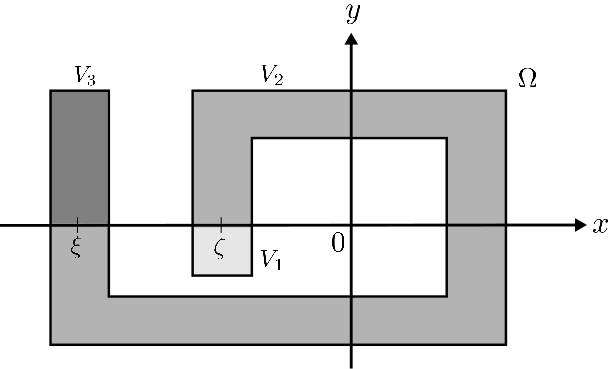
\includegraphics[width=0.65\textwidth]{38.png}
\end{center}

É claro que $0\notin\Omega$ \ e que \textsc{I}nd$_{\gamma}(
0)  =0$ para cada CSDF $\gamma$ em $\Omega$ (se $\gamma$

é uma CSDF em $\Omega,$ então as componentes conexas limitadas de
$\complement\gamma^{\ast}$

estão contidas em $\Omega$ e como $0\notin\Omega$ é claro que $0$
pertence à componente

ilimitada de $\complement\gamma^{\ast},$ logo pelo Teor. 5.2 temos
\textsc{I}nd$_{\gamma}(  0)  =0$). Pela Prop. A.2

existe uma determinação do logaritmo $g$ em $\Omega,$ vamos ver que relações

existem entre $g$ e, por exemplo, as determinações $Log_{k}$ definidas em

$D_{0}=\left\{  z\in%
%TCIMACRO{\U{2102} }%
%BeginExpansion
\mathbb{C}
%EndExpansion
\text{ }|\text{ }z\neq-\left\vert z_{0}\right\vert \right\}  $. Vamos indicar
por $V_{1},V_{2}$ e $V_{3}$ (ver fig.) as três

componentes \ conexas de $\Omega\cap D_{0}.$ Como

\ \ \ \ \ \ \ \ \ \ \ \ \ \ \ \ \ \ \ $\exp\left[  g(  w)  \right]
=w$ \ \ \ \ $\forall$ \ \ \ $w\in\Omega$

\ \ \ \ \ \ \ \ \ \ \ \ \ \ \ \ \ \ \ $\exp\left[  Log(  w)
\right]  =w$ \ \ \ \ \ $\forall$ \ \ \ \ $w\in D_{0}$

\bigskip

é claro que fixada uma componente conexa $V_{\nu}$ \ $(
\nu=1,2,3)  $ \ temos

\bigskip

\ \ \ \ \ \ \ \ \ \ \ \ \ \ \ \ \ $\exp\left[  g(  w)  \right]
=\exp\left[  Log(  w)  \right]  $ \ \ \ \ \ \ $\forall$ \ \ \ $w\in
V_{\nu}$ \ $(  \nu=1,2,3)  $

donde

\ \ \ \ \ \ \ \ \ \ \ \ \ \ \ \ \ $\varphi(  w)  =\dfrac{g(
w)  -Log(  w)  }{2\pi i}\in%
%TCIMACRO{\U{2124} }%
%BeginExpansion
\mathbb{Z}
%EndExpansion
$ \ \ \ \ \ $\forall$ \ \ \ $w\in V_{\nu}$ \ $(  \nu=1,2,3)  $

\bigskip

o que pelo argumento habitual (continuidade de $\varphi,V_{\nu}$ conexo, etc.) implica

que existe $k_{\nu}\in%
%TCIMACRO{\U{2124} }%
%BeginExpansion
\mathbb{Z}
%EndExpansion
$ \ tal que $\varphi(  w)  =k_{\nu}$ \ para cada $w\in V_{\nu},$
isto é

\bigskip

$\left[  1\right]  $ \ \ \ \ \ \ \ \ \ \ \ \ \ \ \ \ \ \ $g(  w)
=Log(  w)  +2k_{\nu}\pi i$ \ \ \ \ $\forall$ \ \ $w\in V_{\nu}$
\ \ $(  \nu=1,2,3)  $

\bigskip

Consideremos agora um ponto $\zeta\in\overline{V}_{1}\cap\overline{V}_{2}%
\cap\Omega.$ Como $g$ é contínua em

$\Omega$ e em particular em $\zeta,$ existe

\bigskip

$\left[  2\right]  $
\ \ \ \ \ \ \ \ \ \ \ \ \ \ \ \ \ \ \ \ \ \ \ \ \ \ \ \ $\underset
{w\rightarrow\zeta}{\lim}g(  w)  =g(  \zeta)  $

\bigskip

A função $Log$ não tem limite para $w\rightarrow\zeta$ porém
é claro que (em vista da

"continuidade lateral" de $Am$)

\bigskip

\ \ \ \ \ \ \ \ \ \ \ \ \ \ \ \ \ \ \ \ $\ \ \ \ \lim$ \ \ $Log(
w)  =$ \ $\lim$ \ $Log(  w)  =\ln\left\vert \zeta\right\vert
+i\pi$

\ \ \ \ \ \ \ \ \ \ \ \ \ \ \ \ \ \ \ \ \ \ \ \ \ \ $\underset
{\text{\textsc{I}}m(  w)  >o}{w\rightarrow\zeta}$
\ \ \ \ \ \ \ \ \ \ \ \ $\underset{w\in V_{2}}{w\rightarrow\zeta}$

\bigskip

\ \ \ \ \ \ \ \ \ \ \ \ \ \ \ \ \ \ \ \ $\lim$ $\ Log(  w)  =$
$\ \ \lim$ $\ Log(  w)  =\ln\left\vert \zeta\right\vert -i\pi$

\ \ \ \ \ \ \ \ \ \ \ \ \ \ \ \ \ \ \ $\underset{\text{\textsc{I}}m(
w)  <0}{w\rightarrow\zeta}$ \ \ \ \ \ \ \ \ \ \ \ \ $\underset{\text{
\ \ }w\in V_{1}\text{ \ \ \ \ }}{w\rightarrow\zeta}$

\bigskip

donde resulta por $\left[  1\right]  :$

\bigskip

$\left[  3\right]  $ \ \ \ \ \ \ \ \ \ \ \ \ \ \ \ \ \ \ \ \ \ $\lim$
$g(  w)  =\ln\left\vert \zeta\right\vert +i\pi+2k_{2}\pi i$

\ \ \ \ \ \ \ \ \ \ \ \ \ \ \ \ \ \ \ \ \ \ \ \ \ $\underset{%
\begin{array}
[c]{c}%
w\in V_{2}\\
\end{array}
}{w\rightarrow\zeta}$

\bigskip$\lbrack4]$\ \ \ \ \ \ \ \ \ \ \ \ \ \ \ \ \ \ \ \ $\underset{%
\begin{array}
[c]{c}%
w\rightarrow\zeta\\
w\in V_{1}%
\end{array}
}{\lim}$ $g(  w)  =\ln\left\vert \zeta\right\vert -i\pi+2k_{1}\pi
i$

\ \ \ \ \ \ \ \ \ \ \ \ \ \ \ \ \ \ \ \ \ \ \ \ \ 

De $\left[  2\right]  ,\left[  3\right]  $ e $\left[  4\right]  $ \ resulta

\ \ \ \ \ \ \ \ \ \ \ \ \ \ \ \ \ \ \ \ \ \ \ \ \ \ \ \ \ \ \ $g(
\zeta)  =\ln\left\vert \zeta\right\vert +i\pi+2k_{2}\pi i=\ln\left\vert
\zeta\right\vert -i\pi+2k_{1}\pi i$

ou seja

\ \ \ \ \ \ \ \ \ \ \ \ \ \ \ \ \ \ \ \ \ \ \ \ \ \ \ \ \ \ $\ \ \ \ \ \ k_{1}%
=k_{2}+1$ $.$

\bigskip

O mesmo raciocínio feito num ponto $\xi\in\overline{V_{2}}\cap
\overline{V_{3}}\cap\Omega$ \ mostra que

\ \ \ \ \ \ \ \ \ \ \ \ \ \ \ \ \ \ \ \ \ \ \ \ \ \ \ \ \ \ \ \ \ \ 

\ \ \ \ \ \ \ \ \ \ \ \ \ \ \ \ \ \ \ \ \ \ \ \ \ \ \ \ \ \ \ \ \ \ \ $k_{2}%
=k_{3}+1$ $,$

donde por $\left[  1\right]  $ resulta

\bigskip\ \ \ \ \ \ \ \ \ \ \ \ \ \ \ \ \ $g(  w)  =\left\{
\begin{array}
[c]{c}%
Log(  w)  +2k_{1}\pi i=Log_{k_{1}}(  w)  \text{
\ \ \ \ }\forall\text{ \ \ \ }w\in V_{1}\text{ \ }\\
Log(  w)  +2k_{2}\pi i=Log_{k_{1}-1}(  w)  \text{
\ \ \ \ }\forall\text{ \ \ }w\in V_{2}\text{ }\\
Log(  w)  +2k_{3}\pi i=Log_{k_{1}-2}(  w)  \text{
\ \ \ \ }\forall\text{ \ \ }w\in V_{3}\text{ }.
\end{array}
\right.  $

\bigskip

\bigskip

\ \ \ \ \ \ \ \ \ \ \ \ \ \ \ \ \ \ \ \ \ \ \ \ \ \ \ \ \ \ \ \ \ \ \ \ \ \ \ \ \ \ \ \ \ \ \ \ \ \ \ \ \ \ \ \ \ \ \ \ \ \ \ \ \ \ 

\ \ \ \ \ \ \ \ \ \ \ \ \ \ \ \ \ \ \ \ \ \ \ \ \ \ \ \ \ \ \ \ 

\bigskip
\ \ \ \ \ \ \ \ \ \ \ \ \ \ \ \ \ \ \ \ \ \ \ \ \ \ \ \ \ \ \ \ \ \ \ \ \ \ \ \ \ \ \ \textbf{Exercícios}%


\bigskip

\bigskip

\textbf{(7.1)} \ (Exerc. de Álgebra) \ Sejam $A$ um anel unitário e
comutativo e $T$ um

conjunto não vazio qualquer. Um aplicação $x:t\in T\longmapsto
x_{t}\in A$ é dita, de

\textit{suporte finito} se o conjunto $\left\{  t\in T\text{ }|\text{ }%
x_{t}\neq0\right\}  $ é finito (e a família $x=(  x_{t})
_{t\in T}$

é dita \textit{quase-nula})\textit{. }Indicamos com $A^{(  T)
} $ o conjunto de todas as aplicações

de $T$ em $A$ de suporte finito, munido das operações pontuais

\bigskip

$(  x_{t})  _{t\in T}+(  y_{t})  _{t\in T}:=(
x_{t}+y_{t})  _{t\in T}$ \ \ \ \ \ e \ \ \ \ \ \ $\lambda(
x_{t})  _{t\in T}:=(  \lambda x_{t})  _{t\in T}$
\ \ \ \ $(  \lambda\in A)  $

\bigskip

Para cada $t\in T$ definimos $e_{t}:=(  \delta_{tt^{\prime}})
_{t^{\prime}\in T}$ \ \ ($\delta_{tt^{\prime}}$ é o $\delta$ de Kronecker).

(a) \ Prove que $A^{(  T)  }$ é um $A$-módulo e que
$(  e_{t})  _{t\in T}$ é uma base de $A^{(  T)  };$

(b) \ Mostre que a aplicação $\beta:t\in T\longmapsto e_{t}\in
A^{(  T)  }$ é injetora e que

portanto $A^{(  T)  }$ pode ser considerado um $A$-módulo de
base $T$ \ (quando

identificamos $t$ com $e_{t}$ pela aplicação $\beta$ resulta $T\subset
A^{(  T)  }$ e portanto

cada elemento de $A^{(  T)  }$\textit{\bigskip\ }admite uma
expressão única do tipo $\underset{t\in T}{%
%TCIMACRO{\dsum }%
%BeginExpansion
{\displaystyle\sum}
%EndExpansion
}x_{t}\cdot t,$

o que justifica o nome que às vezes é dado a $A^{(  T)  }$
que é: \textit{módulo das}

\textit{combinações lineares formais de elementos de }$T$ \textit{com
coeficientes em}

$A.$ O nome mais usual de $A^{(  T)  }$ é o seguinte:
$A$\textit{-módulo livre sobre }$T$);

(c) \ Verifique a seguinte \ "\textit{propriedade universal}" de $A^{(
T)  }:$ para cada $A$-

módulo $X$ e para cada \textit{aplicação }$\varphi:T\rightarrow
X,$ existe uma única \textit{aplicação}

\textit{linear }$\varphi_{\ast}:A^{(  t)  }\rightarrow X$ tal que
$\varphi=\varphi_{\ast}\circ\beta$ (onde $\beta$ é a aplicação
definida em

(b));

(d) \ Mostre que $\varphi_{\ast}$ é injetora (resp. sobrejetora, bijetora)
se e só se

$(  \varphi(  t)  )  _{t\in T}$ é LI (resp. um
sistemas de geradores, uma base) de $X.$

(e) \ Considere o seguinte resultado bem conhecido do primeiro curso de

Álgebra Linear:

\textbf{Proposição: \ }\textit{Se }$K$ \textit{é um corpo e }$V,W
$ \textit{são dois }$K$-\textit{espaços vetoriais de}

\textit{dimensão finita, então qualquer aplicação }%
$K$-\textit{linear }$\theta:V\rightarrow W$ \ \textit{fica deter-}

\textit{minada pelos valores }$\theta(  b_{i})  \in W$ \ $(
1\leq i\leq n)  ,$ \textit{onde }$(  b_{i})  _{1\leq i\leq
n}$ \textit{\ é uma base }

\textit{arbitrária de }$V.$

Mostre que a Proposição acima é um caso particular da propriedade uni-

versal (c). \ No caso particular $A=%
%TCIMACRO{\U{2124} }%
%BeginExpansion
\mathbb{Z}
%EndExpansion
,$ o $%
%TCIMACRO{\U{2124} }%
%BeginExpansion
\mathbb{Z}
%EndExpansion
$-módulo $%
%TCIMACRO{\U{2124} }%
%BeginExpansion
\mathbb{Z}
%EndExpansion
^{(  T)  }$ é chamado \textit{grupo }


% imagem pag157

\begin{wrapfigure}{r}{0.25\textwidth}
  \begin{center}
    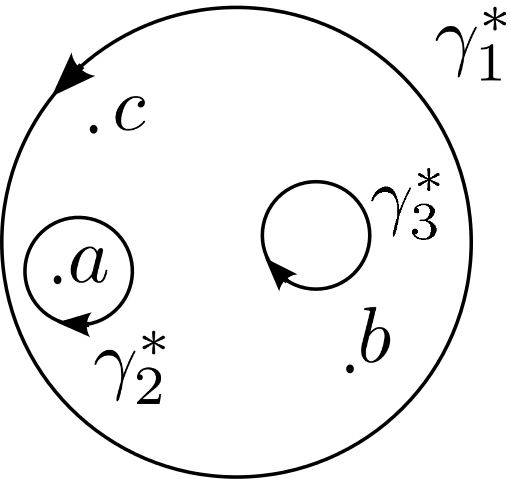
\includegraphics[width=0.25\textwidth]{pag157.png}
  \end{center}
\end{wrapfigure}


\textit{abeliano livre sobre }$T.$

\bigskip\ \ \ \ \ \ \ \ \ \ \ \ \ \ \ \ \ \ \ \ \ \ \ \ \ \ \ \ \ \ \ \ \ \ \ \ \ \ \ \ \ \ \ \ \ \ \ \ \ \ \ \ \ \ \ \ \ \ \ \ \ \ \ \ \ \ \ \ \ \ \ \ \ \ \ \ \ \ \ \ \ \ \ \ \ \ \ \ \ \ \ \ \ \ \ \ \ \ \ \ \ \ \ \ \ \ \ \ \ \ \ \ \ \ \ \ 

\textbf{(7.2) \ }Se consideram os círculos orientados

$\gamma_{1},\gamma_{2}$ e $\gamma_{3}$ da figura ao lado. Sejam

$\Gamma:=\gamma_{1}+\gamma_{2}+\gamma_{3}$ \ \ e \ \ \ $V:=\left\{  z\in%
%TCIMACRO{\U{2102} }%
%BeginExpansion
\mathbb{C}
%EndExpansion
\text{ }|\text{ \textsc{I}nd}_{\Gamma}(  z)  =1\right\}$

(a) \ Prove que se $\Omega$ é um aberto contendo $\overline{V}$ \ e

$f\in\mathcal{H}(  \Omega)  ,$ \ $f\neq0$ \ então

$\ \ \ \ \ \ \ \ \ \ \ \ \ \ \ \ \ \ \ \ \ \ \ \ \ \ \ \ f(  z)
=\dfrac{1}{2\pi i}\underset{\Gamma}{%
%TCIMACRO{\dint }%
%BeginExpansion
{\displaystyle\int}
%EndExpansion
}\dfrac{f(  \zeta)  d\zeta}{\zeta-z}$ \ \ \ $\forall$ \ \ $z\in V$
\ $,$

(b) \ Sejam $\Omega$ e $f$ como em (a) e suponha que $\Omega$

é conexo. Prove que é falsa a afirmação:

\ \ \ \ \ \ \ \ \ \ \ \ \ \ \ \  $f(  z)  =\dfrac
{1}{2\pi i}\underset{\Gamma}{%
%TCIMACRO{\dint }%
%BeginExpansion
{\displaystyle\int}
%EndExpansion
}\dfrac{f(  \zeta)  d\zeta}{\zeta-z}$ \ \ \ \ \ \ $\forall$
\ \ $z\in\Omega\backslash\Gamma^{\ast}$ $,$

(c) \ Sejam $\Omega$ e $f$ como em (a) e sejam $a,b$ e $c$ três pontos de
$\Omega\backslash\Gamma^{\ast}$ como na

figura acima. Determine o valor da integral

\bigskip\ \ \ \ \ \ \ \ \ \ \ \ \ \ \ \ \ \ \ \ \ \ \ \ \textsc{I}
$:=\underset{\Gamma}{%
%TCIMACRO{\dint }%
%BeginExpansion
{\displaystyle\int}
%EndExpansion
}\dfrac{f(  z)  dz}{(  z-a)  (  z-b)  (
z-c)  ^{2}}$ \ $,$

supondo $f(  c)  \neq0.$ \textbf{[Atenção:} \ para fazer
este item (c) sào necessários resul-

tados do Cap. 8 \ (Singularidades).\textbf{]}

\bigskip

\textbf{(7.2}$^{\prime}$\textbf{)} \ \textbf{[}Variante do exerc.
(7.2)\textbf{] \ }Sejam \ $\gamma_{1},\gamma_{2},\gamma_{3},\Gamma
,V,\Omega,a,b$ e $c$ como

no exerc. (7.2) acima e seja $f\in\mathcal{H}(  \Omega)  ,$
$\Omega$ conexo, tal que

\ \ \ \ \ \ \ \ \ \ \ \ \ \ \ \ \ \ \ \ \ \ \ \ \ \ \ $f(  z)
=\underset{\Gamma}{%
%TCIMACRO{\dint }%
%BeginExpansion
{\displaystyle\int}
%EndExpansion
}$\ $\dfrac{e^{i\zeta\text{ }}\operatorname{sen}\zeta}{\zeta-z}d\zeta$
\ \ \ \ \ $\forall$ \ \ $z\in V$ $.$



(a) \ Calcular $f(  p)  $ sendo $p$ um ponto arbitrário da
imagem $\Gamma^{\ast}$ de $\Gamma$ (justifique

todas as passagens);

(b) \ Supondo $\operatorname{sen}a\cdot\operatorname{sen}c\neq0$ determinar o
valor da integral

\ \ \ \ \ \ \ \ \ \ \ \ \ \ \ \ \ \ \ \ \ \ \ \ \ \ \ \textsc{I}
:=$\underset{\Gamma}{%
%TCIMACRO{\dint }%
%BeginExpansion
{\displaystyle\int}
%EndExpansion
}$\ $\dfrac{f(  z)  dz}{(  z-a)  ^{2}(  z-b)
(  z-c)  }$

\textbf{[Atenção:} \ Aqui vale a mesma observação sobre o item
(c) do exerc. (7.2),


isto é, sào necessários resultados do Cap. 8 sobre
singularidades.\textbf{]}

\bigskip

% imagem pag158a

\begin{wrapfigure}{r}{0.2\textwidth}
  \begin{center}
    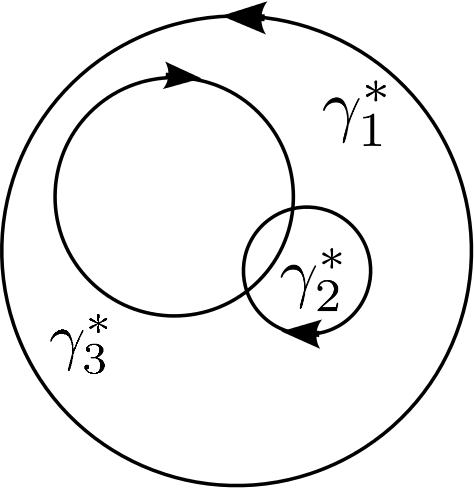
\includegraphics[width=0.2\textwidth]{pag158a.png}
  \end{center}
\end{wrapfigure}


\textbf{(7.2$^{\prime\prime}$)} (Outra variação do exerc. (7.2))

Sejam $\gamma_{1},\gamma_{2}$ e $\gamma_{3}$ os três círculos orientados da figura 

ao lado. Sejam

$\Gamma:=\gamma_{1}+\gamma_{2}+\gamma_{3}$


$W:=\left\{ z\in\mathbb{C}\text{ }|\text{ \textsc{I}nd}_{\Gamma}(z)\neq0\right\}$ e $\Omega$ um aberto

conexo contendo $\overline{W}.$ \ Prove que \underline{não existe}

$f\in\mathcal{H}(  \Omega)  $ \ tal que\\


$f(z)=\underset{\Gamma}{{\displaystyle\int}}\dfrac{e^{i\zeta}\operatorname{sen}\zeta}{\zeta-z}d\zeta$ $\forall$ $z\in W$ $.$\\\\



% imagem pag158b

\begin{wrapfigure}{r}{0.2\textwidth}
  \begin{center}
    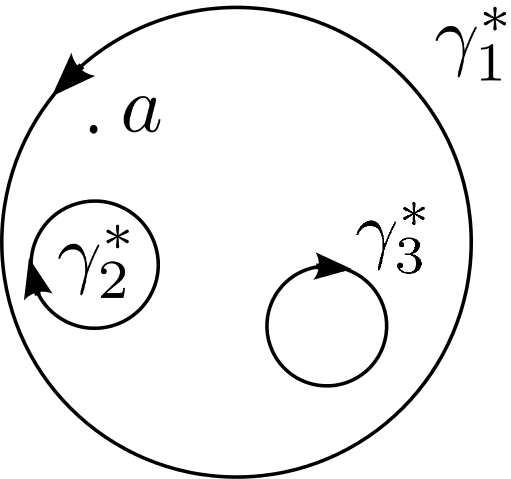
\includegraphics[width=0.2\textwidth]{pag158b.png}
  \end{center}
\end{wrapfigure}

\textbf{(7.2}$^{\prime\prime\prime}$\textbf{) }(Outra variação do exerc. (7.2), usa singulari-

dades)

Se consideram os círculos orientados $\gamma_{1},\gamma_{2}$ e $\gamma_{3}$ da figura

ao lado. Sejam \ $\Gamma:=\gamma_{1}+\gamma_{2}+\gamma_{3},$

$V:=\left\{  z\in\mathbb{C}\text{ }|\text{ \textsc{I}nd}_{\Gamma}(  z)  =1\right\}  $

e \ assuma que $0\in V$ . Suponha dados um aberto conexo 

$\Omega$ contendo \ $\overline{V}$\ \ \ e \ $g\in\mathcal{H}(  \Omega)$.

(a) \ Determine $f\in\mathcal{H}(  \Omega)  $\ \ sabendo que


\bigskip\ \ \ \ \ \ \ \ \ \ \ \ \ \ \ \ \ \ \ \ $f(  z)
$\ $=\underset{\Gamma}{%
%TCIMACRO{\dint }%
%BeginExpansion
{\displaystyle\int}
%EndExpansion
}$\ $\dfrac{g(  \zeta)  (  1-\cos\zeta)  }{\zeta
^{2}(  \zeta-z)  }$\ $d\zeta$\ \ \ \ \ \ \ $\forall$\ \ \ \ \ $z\in
V$\ \ \ $;$\ \ \ \ \ 

(b) \ Seja $a\in V$ \ tal que $a\neq0$ e $g(  a)  (  1-\cos
a\ )  \neq0.$Calcule\ 

\ \ \ \ \ \ \ \ \ \ \ \ \ \ \ \ \ \ \ \ \ \ \ \ \ \ \ \ \ \ \ \ \ \ \textsc{I}
$:=\underset{\Gamma}{%
%TCIMACRO{\dint }%
%BeginExpansion
{\displaystyle\int}
%EndExpansion
}$\ $\ \dfrac{f(  z)  dz}{(  z-a)  ^{2}}$\ $.$\ 

\textbf{[Sugestão:}\ \ (a) \ Sejam $D_{i}$ o disco aberto cuja fronteira
é $\gamma_{1}^{\ast}$ $\ (  1\leq i\leq3)  $

e $W$ a componente conexa não limitada de $\complement\Gamma^{\ast}$
então a figura \ mostra

que as componentes conexas de $\complement\Gamma^{\ast}$ são
$V,D_{2},D_{3}$ e $W$ e, além disso,

que $V=D_{1}\backslash(  \overline{D}_{2}\cup\overline{D}_{3})  .$
A definição de $\Omega$ mostra que $\complement\Omega\subset D_{2}\cup
D_{3}\cup W.$

Conclua que

$(  (  \ast)  )  $%
\ \ \ \ \ \ \ \ \ \ \ \ \ \ \ \ \ \ \ \ \ \ \ \ \ \ \ \ \ \ \ \ \ \ \ \ \ \ $\Gamma
\backsim0$ $\cdot$

A seguir considere a função $h$ definida por

\ \ \ \ \ \ \ \ \ \ \ \ \ \ \ \ \ \ \ \ $h(  z)  :=z^{-2}g(
z)  (  1-\cos z)  $ \ \ \ \ \ $\forall$ \ $z\in
\Omega\backslash\left\{  0\right\}  $

e mostre que \ $h\in\mathcal{H}(  \Omega)  $ \ e

\ \ \ \ \ \ \ \ \ \ \ \ \ \ \ \ \ \ \ \ \ \ \ \ \ \ \ \ \ \ \ $h(
0)  =g(  0)  /2!$ $\cdot$

Aplique o teorema de Cauchy homológico (fórmula de representação

integral à função $h$ (o que é legítimo por $(
(  \ast)  )  :$

\bigskip

\ \ \ \ \ \ \ \ \ \ \ \ \ \ \ \ \ \ \ \ \ \ $h(  z)  =\dfrac
{1}{2\pi i}\underset{\Gamma}{%
%TCIMACRO{\dint }%
%BeginExpansion
{\displaystyle\int}
%EndExpansion
}\dfrac{g(  \zeta)  (  1-\cos\zeta)  }{\zeta^{2}}d\zeta$
\ \ \ $\forall$ \ \ $z\in V$

\bigskip

e deduza que $f(  z)  =2\pi ih(  z)  $ \ \ $\forall$
\ $z\in V.$ Como $\Omega$ é conexo, o Corol. 4.13

acarreta $f=2\pi ih$ em $\Omega$, isto é,

\bigskip

$f(  z)  =2\pi iz^{-2}g(  z)  (  1-\cos z)  $
\ \ $\forall$ \ $z\in\Omega\backslash\left\{  0\right\}  $ \ e \ $f(
0)  =2\pi ih(  0)  =\pi ig(  0)  .$

\bigskip

(b) \ Considere a função $\varphi$ definida por $\varphi(
z)  $ $:=(  z-a)  ^{-2}f(  z)  \ \ \ \forall$
\ $z\in$

$\Omega\backslash\left\{  a\right\}  ,$ é claro que $\varphi$ é
meromorfa\ em $\Omega$ pois $a\in V\subset\Omega$ e como

$a\neq0$ resulta que $a$ é ( o único) polo duplo de $\varphi.$ Como
$\Gamma$ é um ciclo

em $\Omega\backslash\left\{  a\right\}  $ (pois $a\in V$) podemos aplicar o
Teorema dos Resíduos

(ver Corol.7.2 ou Teor. 8.13) obtendo \textsc{I} $=2\pi i$ $\operatorname{Re}%
s(  \varphi,a)  .$ Além disso,

como $a$ é polo duplo é claro que $\operatorname{Re}s(
\varphi,a)  =\dfrac{1}{1!}\psi^{\prime}(  a)  ,$ onde
$\psi(  z)  :=$

$(  z-a)  ^{2}\varphi(  z)  =f(  z)  ,$ donde
$\operatorname{Re}s(  \varphi,a)  =f^{\prime}(  a)  $ e
agora basta então

calcular $f^{\prime}(  z)  $ \ $(  z\neq0)  ,$ oque
resulta derivando a expressão de $f(  z)  $

achada em $(  a)  $\textbf{].}

\ \ \ \ \ \ \ \ \ \ \ \ \ \ \ \ \ \ \ \ \ \ \ \ \ \ \ \ \ \ \ \ \ \ \ \ \ \ \ \ \ \ \ \ \ \ \ \ \ \ \ \ \ \ \ \ \ \ \ \ \ \ \ \ \ \ \ \ \ \ \ 

\ \ \ \ \ \ \ \ \ \ \ \ \ \ \ \ 

\textbf{(7.2}$^{\ast}$\textbf{) }\ Sejam $\gamma$ uma \textit{CSDF }simples
tal que \textsc{I}nd$_{\gamma}(  z)  $ é igual a $0$ ou $1$ para

cada $z\in%
%TCIMACRO{\U{2102} }%
%BeginExpansion
\mathbb{C}
%EndExpansion
\backslash\gamma^{\ast},$ \ $V:=\left\{  z\in%
%TCIMACRO{\U{2102} }%
%BeginExpansion
\mathbb{C}
%EndExpansion
\text{ }|\text{ \textsc{I}nd}_{\gamma}(  z)  =0\right\}  ,$
$\Omega$ um aberto contendo $\overline{V}$ \ e

$f\in\mathcal{H}(  \Omega)  .$

(a) \ Prove que se $\underset{\left\vert z\right\vert \rightarrow+\infty}%
{\lim}f(  z)  =0,$ \ então

\bigskip\ \ \ \ \ \ \ \ \ \ \ \ \ \ \ \ \ \ \ \ \ \ \ \ \ $\dfrac{1}{2\pi
i}\underset{\gamma}{%
%TCIMACRO{\dint }%
%BeginExpansion
{\displaystyle\int}
%EndExpansion
}\dfrac{f(  \zeta)  }{\zeta-z}d\zeta=\left\{
\begin{array}
[c]{c}%
-f(  z)  ,\text{ \ se \ }z\in\Omega\cap V\\
\\
0\text{ },\text{ \ se \ }z\in\Omega\backslash\overline{V}\text{
\ \ \ \ \ \ \ }%
\end{array}
\right.  $

(b) \ Calcule a integral $\dfrac{1}{2\pi i}\underset{\gamma}{%
%TCIMACRO{\dint }%
%BeginExpansion
{\displaystyle\int}
%EndExpansion
}\dfrac{f(  \zeta)  d\zeta}{\zeta-z}$ supondo que $\underset
{\left\vert z\right\vert \rightarrow+\infty}{\lim}f(  z)  =A,$ onde

$A\in%
%TCIMACRO{\U{2102} }%
%BeginExpansion
\mathbb{C}
%EndExpansion
^{\ast}$ é arbitrário \ \textbf{[Sugestão:} \ (a) \ Aplique o
teor. de Cauchy homoló-

gico com um ciclo em $\Omega$ do tipo $\Gamma=\gamma+\gamma_{r},$ sendo
$\gamma_{r}$ um círculo de cen-

tro na origem e raio $r$ suficientemente grande, fazer $r\rightarrow+\infty$
$.$\textbf{]}

\bigskip

\textbf{(7.3)} \ Prove que a homotopia é uma relação de
equivalência \textbf{[}se neces-

sário, ver Dieudonné \cite{D}, Calcul Infinitesimal, pg 203].

\bigskip

\textbf{(7.4) \ [Resultado muito usado!]} \ Sejam $\gamma_{1}$ e $\gamma_{2}$
duas curvas num aberto

$\Omega$ com a mesma origem e o mesmo extremo. Prove que se $\gamma_{1}$ e
$\gamma_{2}$ são

$\Omega$-homotópicas com extremos fixos, então $\gamma_{1}\vee
\gamma_{2}^{\circ}$ é (uma curva fechada)

homotópica a um ponto em $\Omega$ $.$\textbf{[Sugestão: \ }Podemos
supor que $\gamma_{1}$ e $\gamma_{2}$

estão definidas em \textsc{I} $:=\left[  0,1\right]  .$ Seja $h:$
\textsc{I} $\times$ \textsc{I} $\rightarrow\Omega$ uma homotopia de
$\gamma_{1\text{ }}$ a

$\gamma_{2}$ (isto é, $h(  0,t)  =\gamma_{1}(  t)  $
\ e \ $h(  1,t)  =\gamma_{2}(  t)  $ \ $\forall$
\ $t\in$ \textsc{I} e $h(  s,0)  =\gamma_{1}(  0)  =$

$\gamma_{2}(  0)  $ \ e \ $h(  s,1)  =\gamma_{1}(
1)  =\gamma_{2}(  1)  $ \ \ $\forall$ \ $s\in$ \textsc{I} ).
\ Defina uma re-parametriza-

ção $\gamma$ de $\gamma_{1}\vee\gamma_{2}^{\circ}$ da forma seguinte:
$\gamma:$ \textsc{I} $\rightarrow\Omega$ \ é definida por:

\ \ \ \ \ \ \ \ \ \ \ \ $\left\vert
\begin{array}
[c]{c}%
\gamma(  s)  :=\gamma_{1}(  3s)  ,\text{ \ \ }%
\forall\text{ \ }s\in\left[  0,1/3\right]  \text{ },\text{
\ \ \ \ \ \ \ \ \ \ \ \ \ \ \ \ \ \ \ }\\
\gamma(  s)  :=\gamma_{1}(  1)  =\gamma_{2}(
1)  ,\text{ se \ }s\in\left[  1/3,2/3\right]  \text{ \ \ \ \ e}\\
\gamma(  s)  :=\gamma_{2}(  3-3s)  ,\text{ se \ }%
s\in\left[  2/3,1\right]  \text{ \ \ \ \ \ \ \ \ \ \ \ \ \ \ \ \ }%
\end{array}
\right.  $

\bigskip

Prove a seguir que a função $H:$ \textsc{I}$^{2}\rightarrow\Omega$
definida por

\ \ \ \ \ \ \ \ $H(  s,t)  :=\left\{
\begin{array}
[c]{c}%
h(  s,3t(  1-s)  )  ,\text{ \ }\forall\text{ \ }(
t,s)  \in\left[  0,1/3\right]  \times\text{ \textsc{I \ \ \ \ \ \ }}\\
h(  3t-1+2s-3st,1-s)  ,\text{ \ }\forall\text{ \ }(
t,s)  \in\left[  1/3,2/3\right]  \times\text{ \textsc{I}}\\
\gamma_{2}(  (  3-3t)  (  1-s)  )  ,\text{
\ }\forall\text{ \ }(  t,s)  \in\left[  2/3,1\right]  \times\text{
\textsc{I \ \ \ }}%
\end{array}
\right.  $

\bigskip

é uma homotopia de $\gamma$ à curva constante (ponto) $\gamma
_{1}(  0)  =\gamma_{2}(  0)  .$ \textbf{]}

\bigskip


\textbf{(7.5) \ }Sejam $a,b\in%
%TCIMACRO{\U{211d} }%
%BeginExpansion
\mathbb{R}
%EndExpansion
$ com $a>b>0,$ $\gamma_{1}:t\in\left[  0,2\pi\right]  \longmapsto be^{it}\in%
%TCIMACRO{\U{2102} }%
%BeginExpansion
\mathbb{C}
%EndExpansion
$ o círculo

positivamente orientado de centro $O$ e raio $b$ e $\gamma_{2}:t\in\left[
0,2\pi\right]  \longmapsto a\cos t+$

$ib\operatorname{sen}t\in%
%TCIMACRO{\U{2102} }%
%BeginExpansion
\mathbb{C}
%EndExpansion
,$ a elipse \ "positivamente orientada" de centro $O$ e semi-eixos

$a$ e $b$ contidos nos eixos coordenados.

(a) \ Prove que $\gamma_{1}$ e $\gamma_{2}$ são $%
%TCIMACRO{\U{2102} }%
%BeginExpansion
\mathbb{C}
%EndExpansion
$-homotópicas como curvas fechadas;

(b) \ Deduzir que as duas curvas seguintes (agora um círculo e uma elipse

positivamente orientados de centros, raio e semi-eixos arbitrários):

$\gamma_{3}:t\in\left[  0,2\pi\right]  \longmapsto z_{0}+re^{it}\in%
%TCIMACRO{\U{2102} }%
%BeginExpansion
\mathbb{C}
%EndExpansion
$ \ \ e \ \ $\gamma_{4}:t\in\left[  0,2\pi\right]  \longmapsto w_{0}%
+e^{i\theta}\cdot\gamma_{2}(  t)  \in%
%TCIMACRO{\U{2102} }%
%BeginExpansion
\mathbb{C}
%EndExpansion
$

(onde $r>0,$ $0\leq\theta<2\pi$ \ e \ $z_{0},w_{0}\in%
%TCIMACRO{\U{2102} }%
%BeginExpansion
\mathbb{C}
%EndExpansion
$ são dados) são $%
%TCIMACRO{\U{2102} }%
%BeginExpansion
\mathbb{C}
%EndExpansion
$-homotópicas como

curvas fechadas.


\bigskip

\textbf{(7.6)} \ Sejam $a,b\in%
%TCIMACRO{\U{2102} }%
%BeginExpansion
\mathbb{C}
%EndExpansion
,$ $a\neq b,$ $\ \ \Omega:=%
%TCIMACRO{\U{2102} }%
%BeginExpansion
\mathbb{C}
%EndExpansion
\backslash\left\{  a,b\right\}  $ \ e $\gamma$ a CSDF da figura abaixo:
% IMAGEM 34

  \begin{center}
    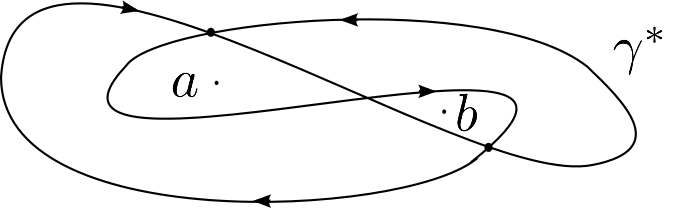
\includegraphics[width=0.5\textwidth]{34.png}
  \end{center}

(a) \ Prove que $\gamma\overset{\Omega}{\backsim}$ $0;$%
\textit{\ \ \ \ \ \ \ \ \ \ \ \ \ \ \ \ \ \ \ \ \ \ \ \ \ \ \ \ \ \ \ \ \ \ \ \ \ \ \ \ \ \ \ \ \ \ \ \ \ \ \ \ \ }%
\textit{\ }

(b) \ É \ "óbvio" que $\gamma$ não é homotópica a um ponto em $\Omega.$ Como você provaria

esta afirmação?

\textbf{[Sugestão:} Cursar tão rápido quanto possível, a
disciplina "Topologia

Algébrica".]

\bigskip

\textbf{(7.7) \ }Sejam $a,b$ e $\gamma_{2}$\textit{\ }como no exerc\textit{.
(7.5) }acima. Calcular de duas\ \ \ 

formas diferentes a integral $\underset{\gamma_{2}}{%
%TCIMACRO{\dint }%
%BeginExpansion
{\displaystyle\int}
%EndExpansion
}$\ $\dfrac{dz}{z} $\ \ e deduzir que

\ \ \ \ \ \ \ \ \ \ \ \ \ \ \ \ \ $\underset{0}{%
%TCIMACRO{\dint }%
%BeginExpansion
{\displaystyle\int}
%EndExpansion
}^{2\pi}$\ $\dfrac{dt}{a^{2}\cos^{2}t+b^{2}\operatorname{sen}^{2}t}%
=\dfrac{2\pi}{ab}$\ $.$

\bigskip

\textbf{(7.8)} \ (a) \ Prove que se $\Omega$ é um aberto simplesmente
conexo então duas

\textit{CSDF }em $\Omega$ são sempre $\Omega$-\textit{HCF}
(homotópicas como curvas fechadas);\\

(b) \ Sejam $m\in%
%TCIMACRO{\U{2124} }%
%BeginExpansion
\mathbb{Z}
%EndExpansion
^{\ast\text{ \ }}$e $\gamma_{m}$\ $:t\in\left[  0,2\pi\right]  \longmapsto
e^{mit}$\ $\in%
%TCIMACRO{\U{2102} }%
%BeginExpansion
\mathbb{C}
%EndExpansion
$ o círculo orientado ("po-

sitivamente" se $m>0$ e "negativamente" se $m<0$) de centro $O$ e raio $1,$

\textit{percorrido }$m$ \textit{vezes}. Prove que $\gamma_{m}$\ e $\gamma_{n}%
$\ são $%
%TCIMACRO{\U{2102} }%
%BeginExpansion
\mathbb{C}
%EndExpansion
$-\textit{HCF }quaisquer que sejam

$m,n\in%
%TCIMACRO{\U{2124} }%
%BeginExpansion
\mathbb{Z}
%EndExpansion
^{\ast}$\ \ e que se $m\neq n$\ então $\gamma_{m}$\ e $\gamma_{n}%
$\ \underline{não}\ são $%
%TCIMACRO{\U{2102} }%
%BeginExpansion
\mathbb{C}
%EndExpansion
^{\ast}$-\textit{HCF}\ ;\\

(c) \ Seja $a\in%
%TCIMACRO{\U{2102} }%
%BeginExpansion
\mathbb{C}
%EndExpansion
,$ prove que $%
%TCIMACRO{\U{2102} }%
%BeginExpansion
\mathbb{C}
%EndExpansion
\backslash\left\{  a\right\}  $\ não é simplesmente conexo;\\

(d) \ Seja $a\in%
%TCIMACRO{\U{2102} }%
%BeginExpansion
\mathbb{C}
%EndExpansion
.$\ Prove que se $\gamma_{1}$\ e\ $\gamma_{2}$\ \ são duas \textit{CSDF}
em $%
%TCIMACRO{\U{2102} }%
%BeginExpansion
\mathbb{C}
%EndExpansion
\backslash\left\{  a\right\}  $\ \ que

são $%
%TCIMACRO{\U{2102} }%
%BeginExpansion
\mathbb{C}
%EndExpansion
\backslash\left\{  a\right\}  $-\textit{HCF}$,$ então \textsc{I}%
nd$_{\gamma_{1}}$\ $(  a)  =$\textsc{I}nd$_{\gamma_{2}}(
a)$  ;\\

(e) \ Se $\Omega\neq%
%TCIMACRO{\U{2102} }%
%BeginExpansion
\mathbb{C}
%EndExpansion
$ é um aberto simplesmente conexo e $\gamma$ é uma \textit{CSDF }em

$\Omega,$ prove que $\gamma\overset{\Omega}{\backsim}0.$

\bigskip

\textbf{(7.9)} \ Lembremos que $D_{0}:=\left\{  z\in%
%TCIMACRO{\U{2102} }%
%BeginExpansion
\mathbb{C}
%EndExpansion
\text{ }|\text{ }z\neq-\left\vert z\right\vert \right\}  $ e $D_{\alpha
}:=e^{i\alpha}\cdot D_{0}$.\\

(a) \ Mostre que $\exp(  \underset{w_{0}}{%
%TCIMACRO{\dint }%
%BeginExpansion
{\displaystyle\int}
%EndExpansion
}^{w}\dfrac{d\zeta}{\zeta})  =\dfrac{w}{w_{0}}$ \ \ $\forall$
\ $w,w_{0}\in D_{0\text{ \ }}$e, em particular

$\exp(  \underset{1}{%
%TCIMACRO{\dint }%
%BeginExpansion
{\displaystyle\int}
%EndExpansion
}^{w}\dfrac{d\zeta}{\zeta})  =w$ \ \ $\forall$ \ $w\in D_{0}$;\\

(b) \ Dados $\alpha\in0,2\pi\lbrack$ \ e $k\in%
%TCIMACRO{\U{2124} }%
%BeginExpansion
\mathbb{Z}
%EndExpansion
,$ mostre que

$\ \ \ \ \ \ \ \ \ \ \ $

$\ \ \ \ \ \ Log_{k,\alpha}(  w)  =i\alpha+Log_{k}(
e^{-i\alpha}w_{0})  +\underset{w_{0}}{%
%TCIMACRO{\dint ^{w}}%
%BeginExpansion
{\displaystyle\int^{w}}
%EndExpansion
}\dfrac{d\zeta}{\zeta} $ \ $,$ \ \ $\forall$ \ $w,w_{0}\in D_{\alpha}$.\\

\bigskip

\textbf{(7.10) \ }(a) \ Calcule a integral $\ \ \ \ \ \ \ \underset{\left\vert
z-1\right\vert =1}{%
%TCIMACRO{\dint }%
%BeginExpansion
{\displaystyle\int}
%EndExpansion
}(  \dfrac{z}{z-1})  ^{m}dz$\ \ \ \ \ \ \ \ 

(b) \ Calcule a integral $\underset{\gamma}{%
%TCIMACRO{\dint }%
%BeginExpansion
{\displaystyle\int}
%EndExpansion
}$\ $\ \dfrac{e^{z}-e^{-z}}{z^{4}}$\ $dz$ $,$ onde $\gamma$ é uma das
seguintes curvas:

% IMAGEM 37

\begin{center}
  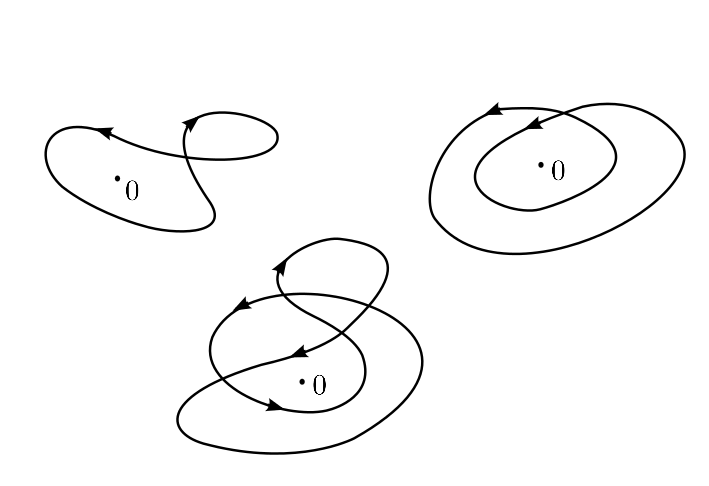
\includegraphics[width=0.6\textwidth]{37.png}
\end{center}


\textbf{[Sugestão:} \ (para (a) e (b)): \ Use o Teor. 7.14].

\bigskip

\textbf{(7.11) \ }Sejam $\gamma$ uma \textit{CSDF} em $%
%TCIMACRO{\U{2102} }%
%BeginExpansion
\mathbb{C}
%EndExpansion
,$ \ $\varphi\in\mathcal{C}(  \gamma^{\ast};%
%TCIMACRO{\U{2102} }%
%BeginExpansion
\mathbb{C}
%EndExpansion
)  $ \ e para cada $m\in%
%TCIMACRO{\U{2115} }%
%BeginExpansion
\mathbb{N}
%EndExpansion
^{\ast},$

considere a função

\ \ \ \ \ \ \ \ \ \ \ \ \ \ \ $F_{m}:z\in\Omega:=%
%TCIMACRO{\U{2102} }%
%BeginExpansion
\mathbb{C}
%EndExpansion
\backslash\gamma^{\ast}\longmapsto\underset{\gamma}{%
%TCIMACRO{\dint }%
%BeginExpansion
{\displaystyle\int}
%EndExpansion
}\dfrac{\varphi(  \zeta)  d\zeta}{(  \zeta-z)  ^{m}}\in%
%TCIMACRO{\U{2102} }%
%BeginExpansion
\mathbb{C}
%EndExpansion
$

Prove que $F_{m}\in\mathcal{H}(  \Omega)  $ e que $F_{m}^{\prime
}(  z)  =mF_{m+1}(  z)  $ \ \ $\forall$ \ $z\in\Omega$
$.$

\textbf{[Sugestão: \ }Este exercício é o Lema 7.13 . \ Se
necessário ver

Conway \cite{C}, pg 92 ou Ahlfors \cite{A}, Cap. IV, \ \S 2, n$^{\underline{o}}$3, \ Lema 3.

\pagebreak

% Capítulo 8

\textbf{{\fontsize{18}{18}\selectfont Capítulo 8\\\\}}

\textbf{{\fontsize{20}{20}\selectfont \ \ \  SINGULARIDADES ISOLADAS. \\}}

\textbf{{\fontsize{20}{20}\selectfont \ \  FUNÇÕES MEROMORFAS. \\}}

\textbf{{\fontsize{20}{20}\selectfont \ \  O TEOREMA DOS RESÍDUOS. \\}}

\textbf{{\fontsize{20}{20}\selectfont \ \  APLICAÇÕES. \\\\\\}}

\bigskip

Basicamente, neste capítulo vamos estudar funções $f\in
\mathcal{H}(  D_{r}^{*}(  a)  )  $ (lembre-

mos que $D_{r}^{*}(  a)  =\left\{  z\in%
%TCIMACRO{\U{2102} }%
%BeginExpansion
\mathbb{C}
%EndExpansion
\text{ }|\text{ }0<\left\vert z-a\right\vert <r\right\}  $) e vamos obter um
certo número

de resultados interessantes a partir da informação sobre o comportamento

de $f$ nas proximidades do ponto $a.$

\bigskip

\textbf{Definição 8.1 \ }Se $\Omega$ é um aberto de $%
%TCIMACRO{\U{2102} }%
%BeginExpansion
\mathbb{C}
%EndExpansion
,$ $a\in%
%TCIMACRO{\U{2102} }%
%BeginExpansion
\mathbb{C}
%EndExpansion
$ e $f\in\mathcal{H(}\Omega\backslash\left\{  a\right\}  )$ dizemos que

$a$ é uma \textit{singularidade isolada de }$f$ (ou que $f$ \textit{tem
uma singularidade isolada }

\textit{em }$a$). Se existe $\varphi\in\mathcal{H}(  \Omega)  $ tal
que $\varphi(  z)  =f(  z)  $ \ \ $\forall$
\ $z\in\Omega\backslash\left\{  a\right\}  $, dizemos

que $a$ é uma \textit{singularidade isolada removível} (ou
simplesmente, \textit{singulari-}

\textit{dade removível}).

\bigskip

\textbf{Exemplo 1} \ Seja $f:z\in%
%TCIMACRO{\U{2102} }%
%BeginExpansion
\mathbb{C}
%EndExpansion
^{\ast}\longmapsto z^{-1}.\operatorname{sen}$ $z$ $\in%
%TCIMACRO{\U{2102} }%
%BeginExpansion
\mathbb{C}
%EndExpansion
$, então $f$ tem uma singula-

ridade removível no ponto $a=0$ pois de

\ \ \ \ \ \ \ \ \ 

\ \ \ \ \ \ \ \ \ \ $\operatorname{sen}z=z-\dfrac{z^{3}}{3!}+\dfrac{z^{5}}%
{5!}-$ $\cdots=z(  1-\dfrac{z^{2}}{3!}+\dfrac{z^{4}}{5!}-\cdots)  $
\ \ $\forall$ \ $z\in%
%TCIMACRO{\U{2102} }%
%BeginExpansion
\mathbb{C}
%EndExpansion
$

\bigskip

resulta que a função inteira $\varphi:z\in%
%TCIMACRO{\U{2102} }%
%BeginExpansion
\mathbb{C}
%EndExpansion
\longmapsto1-\dfrac{z^{2}}{3!}+\dfrac{z^{4}}{5!}-\cdots\in%
%TCIMACRO{\U{2102} }%
%BeginExpansion
\mathbb{C}
%EndExpansion
$ tem a

propriedade $\varphi(  z)  =f(  z)  $ \ \ $\forall$
\ $z\in%
%TCIMACRO{\U{2102} }%
%BeginExpansion
\mathbb{C}
%EndExpansion
^{\ast}.$

\bigskip

\textbf{Proposição 8.2 \ }\textit{Sejam }$\Omega$ \textit{um aberto de
}$%
%TCIMACRO{\U{2102} }%
%BeginExpansion
\mathbb{C}
%EndExpansion
,$ $a\in\Omega$ \textit{e} $f\in\mathcal{H}(  \Omega\backslash\left\{
a\right\}  )  ,$ \textit{então }

\textit{as condições seguintes são equivalentes:}

(i) \ $\ \ a$ \textit{é uma singularidade removível de }$f;$

(ii) \ \ \textit{Existem }$D_{r}(  a)  \subset\Omega$ \textit{e
}$\psi\in\mathcal{H}(  D_{r}(  a)  )  $ \textit{tais que
}$\psi|D_{r}^{*}(  a)  =f$ $|D_{r}^{*}(  a)
;$

(iii) \ \textit{Existe }$D_{r}(  a)  \subset\Omega$ \textit{tal que
}$\left\Vert f\right\Vert _{D_{r}^{*}(  a)  }<+\infty;$

(iv) \ \ $\underset{z\rightarrow a}{\lim}(  z-a)  f(
z)  =0$

\bigskip

\textbf{Prova \ }As implicações (i) $\iff$ (ii) $\implies$ (iii)
$\implies$ (iv) são óbvias portanto

basta mostrar que (iv) $\implies$ (ii). Seja $h:\Omega\rightarrow%
%TCIMACRO{\U{2102} }%
%BeginExpansion
\mathbb{C}
%EndExpansion
$ a função definida por

\ \ \ \ \ \ \ \ \ \ \ \ \ \ \ \ \ \ \ \ \ \ \ \ \ \ $h(  z)
=\left\{
\begin{array}
[c]{c}%
0,\text{ se }z=a\text{ \ \ \ \ \ \ \ \ \ \ \ \ \ }\\
\\
(  z-a)  ^{2}f(  z)  ,\text{ se }z\neq a
\end{array}
\right.  $

\bigskip calculando $h^{\prime}(  a)  $ pela definição, por
(iv) obtemos

\ \ \ \ \ \ \ \ \ \ \ \ \ \ \ \ \ \ \ \ \ \ $h^{\prime}(  a)
=\underset{z\rightarrow a}{\lim}(  z-a)  f(  z)  =0$

o que mostra que $h\in\mathcal{H}(  \Omega)  .$ Como $a$ é um
zero de $h$ (ver Def. 4.17)

existem $D_{r}(  a)  \subset\Omega,$ $\nu\in%
%TCIMACRO{\U{2115} }%
%BeginExpansion
\mathbb{N}
%EndExpansion
^{\ast}$ e$\ g\in\mathcal{H}(  D_{r}(  a)  )  $\ tais
que$\ g(  z)  \neq0$\ para

cada $z\in D_{r}(  a)  $ \ e

$\bigskip(  8.2.1)  $ \ \ \ \ \ \ \ \ \ \ \ \ $h(  z)
=(  z-a)  ^{\nu}g(  z)  $ \ \ $\forall$ \ $z\in
D_{r}(  a)  $

Como $a$ é um zero de $h^{\prime}$ é claro (ver exerc. 4.14) que
$\nu>1$, o que prova

que a função

\ \ \ \ \ \ \ \ \ \ \ \ \ \ \ \ \ \ \ \ \ \ \ \ \ $\psi:z\in D_{r}(
a)  \longmapsto(  z-a)  ^{\nu-2}\cdot g(  z)  \in%
%TCIMACRO{\U{2102} }%
%BeginExpansion
\mathbb{C}
%EndExpansion
$

é holomorfa. É claro que $(  8.2.1)  $ pode ser escrita assim:

\ \ \ \ \ \ \ \ \ \ \ \ \ \ \ \ \ \ \ \ \ \ \ $h(  z)  =(
z-a)  ^{2}\psi(  z)  $ \ \ $\forall$ \ $z\in D_{r}(
a)  $

o que, pela definição de $h,$ implica $f(  z)  =\psi(
z)  $ para cada $z\in D_{r}^{*}(  a)  ,$

o que prova (ii) pois $\psi\in\mathcal{H}(  D_{r}(  a)
)  .$ $\square$

\bigskip

\textbf{Exemplo 2 \ }Seja $f:z\in%
%TCIMACRO{\U{2102} }%
%BeginExpansion
\mathbb{C}
%EndExpansion
^{\ast}\longmapsto\operatorname{sen}(  z^{-1})  \in%
%TCIMACRO{\U{2102} }%
%BeginExpansion
\mathbb{C}
%EndExpansion
.$ A função $f$ tem uma

singularidade isolada em $a=0$ que não é removível. Para prová-lo

usamos a Prop. 8.2 (iii): dado $H>1$ arbitrário, existe $\varepsilon>0$
tal que

$0<x<\varepsilon$ $\implies e^{1/x}$ $>H\implies e^{-1/x}<H^{-1}$ e então,
para cada $z=ix$ tal

que $\ 0<x<\varepsilon$ temos

\ \ \ \ \ \ \ \ \ \ \ \ \ $\left\vert f(  x)  \right\vert
=\dfrac{1}{2}\left\vert e^{1/x}-e^{-1/x}\right\vert >\dfrac{1}{2}\left\vert
H-H^{-1}\right\vert >\dfrac{1}{2}(  H-1)  ,$

isto é, \ $\left\Vert f\right\Vert _{D_{\varepsilon}^{*}(
0)  }=+\infty$ para cada $\varepsilon>0.$ Observemos também que, como

$f(  z)  =0$ se e só se $z=(  k\pi)  ^{-1}$ com
$k\in%
%TCIMACRO{\U{2124} }%
%BeginExpansion
\mathbb{Z}
%EndExpansion
^{\ast},$ se $\Omega:=\{z\in%
%TCIMACRO{\U{2102} }%
%BeginExpansion
\mathbb{C}
%EndExpansion
^{\ast}$ $|$ $z\neq(  k\pi)  ^{-1}$

$\forall$ \ $k\in%
%TCIMACRO{\U{2124} }%
%BeginExpansion
\mathbb{Z}
%EndExpansion
^{\ast}\}$, a função

\ \ \ \ \ \ \ \ \ \ \ \ \ \ \ \ \ \ \ $g:z\in\Omega\longmapsto(  f(
x)  )  ^{-1}=(  \operatorname{sen}(  z^{-1})
)  ^{-1}\in%
%TCIMACRO{\U{2102} }%
%BeginExpansion
\mathbb{C}
%EndExpansion
$

é analítica em $\Omega.$ É fácil ver que para cada $k\in%
%TCIMACRO{\U{2124} }%
%BeginExpansion
\mathbb{Z}
%EndExpansion
^{\ast},$ $g$ tem uma singulari-

dade não removível no ponto $(  k\pi)  ^{-1}$ e em
consequência o ponto $a=0$

é uma \textit{singularidade não isolada de }$g.$ Não estudaremos
aqui este tipo

de singularidades.

\bigskip

\textbf{Observações \ (A) \ }A Prop. 8.2 mostra mais uma diferença interessante

entre funções reais de variável real e funções complexas
de variável com-

plexa. A função $f(  x)  =\left\vert x\right\vert $
\ \ $\forall$ \ $x\in%
%TCIMACRO{\U{211d} }%
%BeginExpansion
\mathbb{R}
%EndExpansion
$ tem uma "singularidade não removível"

no ponto $a=0$ o que não impede de $\left\vert f\right\vert $ ser limitada
em qualquer intervalo

$\left]  -\varepsilon,\varepsilon\right[  .$ Esta situação não
pode acontecer no caso complexo: para uma

função complexa de variável complexa $f$ ter uma singularidade "honesta"

no ponto $a$ (i.e. não removível), $f$ deve ser bastante "mal
comportada" nas

proximidades de $a,$ isto é, não pode existir e ser finito o limite
$\underset{z\rightarrow a}{\lim}\left\vert f(  x)  \right\vert ,$

em outros termos, ou $\underset{z\rightarrow a}{\lim}\left\vert f(
x)  \right\vert =+\infty$ ou este limite não existe.

\textbf{(B) \ }Se $a\in%
%TCIMACRO{\U{2102} }%
%BeginExpansion
\mathbb{C}
%EndExpansion
,$ $\nu\in%
%TCIMACRO{\U{2115} }%
%BeginExpansion
\mathbb{N}
%EndExpansion
^{\ast}$ e $(  c_{k})  _{1\leq k\leq\nu}$ é uma sequência
de números complexos

tal que $c_{\nu}\neq0,$ então: (I) A função

\ \ \ \ \ \ \ \ \ \ \ \ \ \ \ \ \ \ \ \ $\theta:z\in%
%TCIMACRO{\U{2102} }%
%BeginExpansion
\mathbb{C}
%EndExpansion
\backslash\left\{  a\right\}  \longmapsto\underset{k=1}{\overset{\nu}{%
%TCIMACRO{\dsum }%
%BeginExpansion
{\displaystyle\sum}
%EndExpansion
}}c_{k}(  z-a)  ^{-k}\in%
%TCIMACRO{\U{2102} }%
%BeginExpansion
\mathbb{C}
%EndExpansion
$

tem uma singularidade não removível em $a;$ (II) \ Se $\Omega$ é
um aberto de $%
%TCIMACRO{\U{2102} }%
%BeginExpansion
\mathbb{C}
%EndExpansion
,$

$a\in\Omega,$ $f\in\mathcal{H}(  \Omega\backslash\left\{  a\right\}
)  $ e $f-\theta|\Omega\backslash\left\{  a\right\}  $ tem uma
singularidade removível em

$a,$ então $f$ tem uma singularidade não removível em $a.$

De fato, suponhamos por absurdo que $\theta$ tem uma singularidade removí-

vel em \ então

\bigskip

(B.1) \ \ \ \ \ \ \ $\exists$ \ $\ F\in\mathcal{H}(
%TCIMACRO{\U{2102} }%
%BeginExpansion
\mathbb{C}
%EndExpansion
)  $ tal que $F(  z)  =\overset{\nu}{\underset{k=1}{%
%TCIMACRO{\dsum }%
%BeginExpansion
{\displaystyle\sum}
%EndExpansion
}}c_{k}(  z-a)  ^{-k}$ \ \ \ $\forall$ \ $z\in%
%TCIMACRO{\U{2102} }%
%BeginExpansion
\mathbb{C}
%EndExpansion
\backslash\left\{  a\right\}  $

donde multiplicando por $(  z-a)  ^{\nu}$ resulta

\ \ \ \ \ \ \ \ \ \ \ \ \ \ \ \ \ $F(  z)  (  z-a)
^{\nu}=\overset{\nu}{\underset{k=1}{%
%TCIMACRO{\dsum }%
%BeginExpansion
{\displaystyle\sum}
%EndExpansion
}}c_{k}(  z-a)  ^{\nu-k}+c_{\nu}$ \ \ $\forall$ \ $z\in%
%TCIMACRO{\U{2102} }%
%BeginExpansion
\mathbb{C}
%EndExpansion
\backslash\left\{  a\right\}  $

portanto tomando limites para $z\rightarrow a$ obtemos $c_{\nu}=0,$ contra o suposto,

o que prova (I). Como por hipótese $f-\theta|\Omega\backslash\left\{
a\right\}  $ tem uma singularidade

removível em $a,$ existe $\psi\in\mathcal{H}(  \Omega)  $ tal
que $f(  z)  -\theta(  z)  =\psi(  z)  $
\ \ $\forall$ \ $z\in\Omega\backslash\left\{  a\right\}  .$

Se $f$ tivesse uma singularidade removível em $a,$ então existiria
$\varphi\in\mathcal{H}(  \Omega)  $

tal que $f(  z)  =\varphi(  z)  $ \ \ $\forall$
\ $z\in\Omega\backslash\left\{  a\right\}  ,$ o que implica $\theta(
z)  =+\varphi(  z)  -\psi(  z)  $

$\forall$ \ $z\in\Omega\backslash\left\{  a\right\}  ,$ donde resultaria que
$\theta$ tem uma singularidade removível em

$a$ (pois $-\varphi-\psi\in\mathcal{H}(  \Omega)  $), o que é
absurdo por (I). Isto prova (II).

\bigskip

O resultado seguinte classifica os três tipos de singularidades isoladas

possíveis.

\bigskip

\textbf{Teorema 8.3} \ \textit{Sejam }$\Omega$ \textit{um aberto de }$%
%TCIMACRO{\U{2102} }%
%BeginExpansion
\mathbb{C}
%EndExpansion
,$ $a\in\Omega$ \textit{e }$f\in\mathcal{H}(  \Omega\backslash\left\{
a\right\}  )  ,$ \textit{então se }

\textit{verifica uma e apenas uma das três condições seguintes:}

(a) \ $f$ \textit{tem uma singularidade removível no ponto }$a.$

(b) \ \textit{Existem um único }$\nu\in%
%TCIMACRO{\U{2115} }%
%BeginExpansion
\mathbb{N}
%EndExpansion
^{\ast}$ \textit{e uma única sequência }$(  c_{k})  _{1\leq
k\leq\nu}$ \textit{de núme-}

\textit{ros complexos tal que }$c_{\nu}\neq0,$ \textit{de modo que a
função}

\ \ \ \ \ \ \ \ \ \ \ \ \ \ \ \ $z\in\Omega\backslash\left\{  a\right\}
\longmapsto f(  z)  -\overset{\nu}{\underset{k=1}{%
%TCIMACRO{\dsum }%
%BeginExpansion
{\displaystyle\sum}
%EndExpansion
}}c_{k}(  z-a)  ^{-k}\in%
%TCIMACRO{\U{2102} }%
%BeginExpansion
\mathbb{C}
%EndExpansion
$

\textit{tem uma singularidade removível no ponto }$a.$

(c) \ \textit{Para cada }$\rho>0$ \textit{tal que }$D_{\rho}(  a)
\subset\Omega,$ \textit{o conjunto }$f(  D_{\rho}^{*}(
a)  )  $ \textit{é denso }

\textit{em }$%
%TCIMACRO{\U{2102} }%
%BeginExpansion
\mathbb{C}
%EndExpansion
.$

\bigskip

\textbf{Prova \ }Indicamos com $\backsim(  c)  $ a negação
de $(  c)  $ (significado análogo para

as notações $\backsim(  a)  $ e $\thicksim(  b)
$). Então é claro que basta provar as duas impli-

cações seguintes:

\bigskip

$(  8.3.1)  $ \ \ \ \ \ \ \ \ \ \ \ \ \ \ \ \ $(  c)
\implies$ $\backsim(  a)  $ e $\backsim(  b)  $ \ 

$(  8.3.2)  $ \ \ \ \ \ \ \ \ \ \ \ \ $\backsim(  c)
\implies$ ou $(  a)  $ ou $(  b)  $

\bigskip

Pela Prop. 8.2 \ (i) $\iff$(iii) é claro que $(  c)
\implies\backsim(  a)  $ portanto, para provar

$(  8.3.1)  $ basta mostrar que $(  c)  \implies
\backsim(  b)  $ ou equivalentemente

\bigskip

$(  8.3.1^{\prime})  $ \ \ \ \ \ \ \ \ \ \ \ \ \ \ \ \ $(
b)  \implies\backsim(  c)  $ $.$

\bigskip

Pela observação (B), (II) precedente é claro que

\ \ \ \ \ \ \ \ \ \ \ \ \ \ \ \ \ \ \ $(  a)  \implies
\backsim(  b)  $ \ \ (Ou equivalentemente \ $(  b)
\implies\backsim(  a)  $)$,$

isto é, as condições (a) e (b) não se verificam
simult\^{a}neamente . Resulta

então que para provar $(  8.3.2)  $ é suficiente mostrar a implicação

\bigskip

$(  8.3.2^{\prime})  $ \ \ \ \ \ \ \ \ \ \ \ $\backsim(
c)  \implies(  a)  $ ou $(  b)  $

\bigskip

Desta forma, a prova do resultado se reduz a verificar $(  8.3.1^{\prime
})  $ e $(  8.3.2^{\prime})  .$

\bigskip

\textbf{Prova de }$(  8.3.2^{\prime})  $ \ Se $(  c)  $
é falso, então existem $\rho>0,$ $\delta>0$ e $w\in%
%TCIMACRO{\U{2102} }%
%BeginExpansion
\mathbb{C}
%EndExpansion
$ tais

que

\ \ \ \ \ \ \ \ \ \ \ \ \ \ \ \ \ \ \ \ $D_{\rho}(  a)
\subset\Omega$ \ e \ $f(  z)  \notin\overline{D}_{\delta}(
w)  $ \ \ $\forall$ \ $z\in D_{\rho}^{*}(  a)  $

ou seja

\ \ \ \ \ \ \ \ \ \ \ \ \ \ \ \ \ \ \ \ \ \ $\left\vert f(  z)
-w\right\vert >\delta$ \ \ $\forall$ \ $z\in D_{\rho}^{*}(
a)  .$

Consideremos a função

\ \ \ \ \ \ \ \ \ \ \ \ \ \ \ \ \ \ \ \ \ \ \ $g:z\in D_{\rho}^{*}(
a)  \longrightarrow\dfrac{1}{f(  z)  -w}\in%
%TCIMACRO{\U{2102} }%
%BeginExpansion
\mathbb{C}
%EndExpansion
$ $.$

É claro que $g\in\mathcal{H}(  D_{\rho}^{*}(  a)
)  $ e $\left\vert g(  z)  \right\vert <\delta^{-1}$
\ \ $\forall$ \ $z\in D_{\rho}^{*}(  a)  ,$ logo, pela Prop.

8.2. (iii)$\implies$(i), $g$ tem uma singularidade removível em $a$ e
portanto existe

$\psi\in\mathcal{H}(  D_{\rho}(  a)  )  $ tal que
$\psi|D_{\rho}^{*}(  a)  =g.$ Temos então dois casos possíveis

segundo que $\psi(  a)  =0$ ou $\psi(  a)  \neq0.$

\bigskip

\textbf{Caso 1: } \ $\psi(  a)  \neq0.$ \ Neste caso, como
$\psi\neq0$ (pois $g\neq0$), pelo Teor. 4.15

existe $r>0$ tal que $D_{r}(  a)  \subset D_{\rho}(  a)
$ e $\psi(  z)  \neq0$ \ \ $\forall\ \ z\in D_{r}(  a)
.$ Em

consequência podemos considerar a seguinte função

\ \ \ \ \ \ \ \ \ \ \ \ \ \ \ \ \ \ \ \ \ $\varphi:z\in D_{r}(  a)
\longmapsto w+\dfrac{1}{\psi(  z)  }\in%
%TCIMACRO{\U{2102} }%
%BeginExpansion
\mathbb{C}
%EndExpansion
$

É claro que $\varphi\in\mathcal{H}(  D_{r}(  a)  )
. $ A relação $\psi|D_{\rho}^{*}(  a)  =g$ implica
$\psi|D_{r}^{*}(  a)  =$

$g|D_{r}^{*}(  a)  $ e então as definições de
$\varphi$ e de $g$ mostram que $\varphi|D_{r}^{*}(  (
a)  )  =f|D_{r}^{*}(  a)  $,

o que prova pela Prop. 8.2. (ii) $\implies$(i), que neste caso se verifica
$(  a)  $.

\bigskip

\textbf{Caso 2: \ }$\psi(  a)  =0$ \ Neste caso, como $a$ é um
zero de $\psi$ (ver Def. 4.17)

existem $D_{r}(  a)  \subset D_{\rho}(  a)  ,$ $\nu\in%
%TCIMACRO{\U{2115} }%
%BeginExpansion
\mathbb{N}
%EndExpansion
^{\ast}$ e $\psi_{0}\in\mathcal{H}(  D_{r}(  a)  )  $
tais que $\psi_{0}(  z)  \neq0$ \ \ 

$\forall$ \ $z\in D_{r}(  a)  $ e

\ \ \ \ \ \ \ \ \ \ \ \ \ \ \ \ \ \ \ \ \ \ \ \ \ \ $\psi(  z)
=(  z-a)  ^{\nu}\cdot\psi_{0}(  z)  $ \ \ $\forall$
\ $z\in D_{r}(  a)  .$

Como $\psi_{0}$ não tem zeros em $D_{r}(  a)  ,$ a função

\ \ \ \ \ \ \ \ \ \ \ \ \ \ \ \ \ \ \ \ \ \ \ \ \ \ $h:z\in D_{r}(
a)  \longmapsto\dfrac{1}{\psi_{0}(  z)  }\in%
%TCIMACRO{\U{2102} }%
%BeginExpansion
\mathbb{C}
%EndExpansion
$

é analítica em $D_{r}(  a)  $ e podemos portanto
considerar o seu desenvolvimento

de Taylor em volta de $a$ (ver Corol. 4.11):

\bigskip

$(  8.3.3)  $ \ \ \ \ \ \ \ \ \ \ \ \ \ \ $h(  z)
=\underset{m\geq0}{%
%TCIMACRO{\dsum }%
%BeginExpansion
{\displaystyle\sum}
%EndExpansion
}b_{m}(  z-a)  ^{m}$ \ \ $\forall$ \ $z\in D_{r}(  a)  $
$\cdot$

\bigskip

Por outro lado, a definição de $\psi$ e a relação
$D_{r}^{*}(  a)  \subset D_{\rho}^{*}(  a)  $ \ implicam

\ \ \ \ \ \ \ \ $g(  z)  =\psi(  z)  =(
z-a)  ^{\nu}\psi_{0}(  z)  =\dfrac{1}{(  z-a)
^{-\nu}\cdot h(  z)  }$ \ \ $\forall$ $\ z\in D_{r}^{*}(
a)  $

donde, pela definição de $g$ resulta:

\bigskip

$(  8.3.4)  $ \ \ \ \ \ \ \ \ \ $f(  z)  -w=(
z-a)  ^{-\nu}\cdot h(  z)  $ \ \ $\forall$ \ $z\in
D_{r}^{*}(  a)  $

\bigskip

De $(  8.3.3)  $ e $(  8.3.4)  $ segue que para cada
$z\in D_{r}^{*}(  a)  $ temos:

\bigskip

$f(  z)  -w=\dfrac{b_{0}}{(  z-a)  ^{\nu}}+\dfrac{b_{1}%
}{(  z-a)  ^{\nu-1}}+$ $\ldots$ $+\dfrac{b_{\nu-1}}{z-a}+b_{\nu
}+b_{\nu+1}(  z-a)  +$ $\ldots$

\bigskip

e então, pondo $c_{k}:=b_{\nu-k}$ para $k=1,2,$ $\ldots$ $\nu$, podemos escrever

\bigskip

$(  8.3.5)  $ \ \ \ $f(  z)  -\underset{k=1}%
{\overset{\nu}{%
%TCIMACRO{\dsum }%
%BeginExpansion
{\displaystyle\sum}
%EndExpansion
}}c_{k}(  z-a)  ^{-k}=w+b_{\nu}+b_{\nu+1}(  z-a)  +$
$\ldots$ , \ \ $\forall$ \ $z\in D_{r}^{*}(  a)  $

\bigskip

e $c_{\nu}=b_{\nu}=h(  a)  \neq0.$ Além disto, o 2$^{\underline
{o}}$ membro de $(  8.3.5)  $ está definido

em $D_{r}(  a)  $ e portanto (ver exerc. 5.10) define uma
função $F\in\mathcal{H}(  D_{r}(  a)  )  $

e então $(  8.3.5)  $ implica que

\ \ \ \ \ \ \ \ \ \ \ \ \ \ \ \ \ \ \ \ \ \ \ \ \ $z\in\Omega\backslash
\left\{  a\right\}  \longmapsto f(  z)  -\overset{\nu}%
{\underset{k=1}{%
%TCIMACRO{\dsum }%
%BeginExpansion
{\displaystyle\sum}
%EndExpansion
}}c_{k}(  z-a)  ^{-k}\in%
%TCIMACRO{\U{2102} }%
%BeginExpansion
\mathbb{C}
%EndExpansion
$

tem uma singularidade removível em $a.$ Para verificarmos que neste caso

vale a condição (b), só resta mostrar a unicidade de $\nu$ e dos coeficientes

$c_{k}.$ Suponhamos por absurdo que existem duas funções $F_{1}%
,F_{2}\in\mathcal{H}(  \Omega)  $

e duas sequências finitas de números complexos $(  c_{k})
_{1\leq k\leq\nu}$ e $(  c_{j}^{\prime})  _{1\leq j\leq\mu}$

tais que

\bigskip$(  8.3.6)  $ \ \ \ \ \ $f(  z)  -\underset
{k=1}{\overset{\nu}{%
%TCIMACRO{\dsum }%
%BeginExpansion
{\displaystyle\sum}
%EndExpansion
}}c_{k}(  z-a)  ^{-k}=F_{1}(  z)  $ \ \ $\forall$
\ $z\in\Omega\backslash\left\{  a\right\}  ,$ \ $c_{\nu}\neq0 $

\bigskip

$(  8.3.7)  $ \ \ \ \ \ $f(  z)  -\overset{\mu
}{\underset{j=1}{%
%TCIMACRO{\dsum }%
%BeginExpansion
{\displaystyle\sum}
%EndExpansion
}}c_{j}^{\prime}(  z-a)  ^{-j}=F_{2}(  z)  $
\ \ $\forall$ \ $z\in\Omega\backslash\left\{  a\right\}  ,$ \ \ $c_{\mu
}^{\prime}\neq0$

\bigskip então vamos provar que

\bigskip

$(  8.3.8)  $ \ \ \ \ \ \ \ \ \ \ \ \ \ \ \ \ \ \ $\nu=\mu$ \ \ \ e
\ \ \ $c_{k}=c_{k}^{\prime}$ \ \ $\forall$ \ $k=1,2,$ $\ldots,$ $\nu$

\bigskip

É claro que não há perda de generalidade em supor, por exemplo, que

$\mu\geq\nu,$ então subtraindo $(  8.3.7)  $ de $(
8.3.6)  $ podemos escrever

\bigskip

$(  8.3.9)  $ \ \ \ \ \ \ \ \ \ \ \ \ \ \ \ \ $F(  z)
=\underset{r=1}{\overset{\mu}{%
%TCIMACRO{\dsum }%
%BeginExpansion
{\displaystyle\sum}
%EndExpansion
}}\dfrac{d_{r}}{(  z-a)  ^{r}}$ \ \ \ \ $\forall$ \ $z\in
\Omega\backslash\left\{  a\right\}  $

\bigskip

onde $F:=F_{1}-F_{2}$ \ \ e

\bigskip\ \ \ \ \ \ \ \ \ \ \ \ \ \ \ \ \ \ \ \ \ \ \ \ \ \ \ \ \ \ \ \ $d_{r}%
:=\left\{
\begin{array}
[c]{c}%
c_{r}^{\prime}-c_{r},\text{ \ se \ }1\leq r\leq\nu\\
\\
c_{r}^{\prime},\text{ \ se \ }v<r\leq\mu\text{ \ \ \ \ \ }%
\end{array}
\right.  $.

\bigskip

Como $F\in\mathcal{H}(  \Omega)  ,$ o mesmo argumento usado na Obs.
(B), (I) para

mostrar que (B.1) é falsa, implica que $(  8.3.9)  $ é
falsa a menos que

$d_{r}=0$ para cada $r=1,2,$ $\ldots,\mu.$ Ora, como $c_{\nu}\neq0$ e $c_{\mu
}^{\prime}\neq0,$ resulta

$\mu=\nu$ e $c_{r}=c_{r}^{\prime}$ para cada $r=1,2,\ldots,\nu,$ o que prova
$(  8.3.8)  .$ Isto

completa a verificação de que no Caso 2 vale a condição (b), o que

prova $(  8.3.2^{\prime})  .$

\bigskip

\textbf{Prova de }$(  8.3.1^{\prime})  $ \ A hipótese (b)
implica que existe $\varphi\in\mathcal{H}(  \Omega)  $ tal que

\bigskip

$(  8.3.10)  $ \ \ \ \ \ \ \ \ \ \ $\varphi(  z)
=f(  z)  -\overset{\nu}{\underset{k=1}{%
%TCIMACRO{\dsum }%
%BeginExpansion
{\displaystyle\sum}
%EndExpansion
}}\dfrac{c_{k}}{(  z-a)  ^{k}}$ \ \ \ $\forall$ \ $z\in
\Omega\backslash\left\{  a\right\}  $

\bigskip

Fixado $\varepsilon>0$ arbitrário, a continuidade de $\varphi$ implica que
existe $\delta_{1}>0$

tal que

\bigskip

$(  8.3.11)  $ \ \ \ \ \ \ \ \ \ \ \ \ \ $z\in D_{\delta_{1}%
}(  a)  \implies\left\vert \varphi(  z)  -\varphi(
a)  \right\vert <\varepsilon$

\bigskip

Seja

\bigskip\ \ \ \ \ \ \ \ \ \ \ \ \ \ \ \ \ \ \ \ \ \ \ \ $T(  z)
:=\left\vert \dfrac{c_{\nu}}{(  z-a)  ^{\nu}}\right\vert
-\left\vert \underset{k=1}{\overset{\nu-1}{%
%TCIMACRO{\dsum }%
%BeginExpansion
{\displaystyle\sum}
%EndExpansion
}}\dfrac{c_{k}}{(  z-a)  ^{k}}\right\vert $
\ \ \ \ \ \ \ \ $(  z\neq a)  $

e mostremos que

\bigskip

$(  8.3.12)  $
\ \ \ \ \ \ \ \ \ \ \ \ \ \ \ \ \ \ \ \ \ \ \ $\underset{z\rightarrow a}{\lim
}T(  z)  =+\infty$

\bigskip

De fato,

\ \ \ \ \ \ \ \ \ \ \ \ \ $T(  z)  =\left\vert \dfrac{z-a}%
{z-a}\right\vert ^{\nu}T(  z)  =\dfrac{1}{\left\vert z-a\right\vert
^{\nu}}\left[  \left\vert c_{\nu}\right\vert -\left\vert \underset
{k=1}{\overset{\nu-1}{%
%TCIMACRO{\dsum }%
%BeginExpansion
{\displaystyle\sum}
%EndExpansion
}}c_{k}(  z-a)  ^{\nu-k}\right\vert \right]  $

\bigskip

e como $\left\vert c_{\nu}\right\vert >0$ e $\nu-k>0$ sempre que $1\leq
k\leq\nu-1,$ resulta que para

$z$ suficientemente próximo de $a$ temos

\bigskip

\ \ \ \ \ \ \ \ \ \ \ \ \ \ $\left\vert c_{\nu}\right\vert -\left\vert
\overset{\nu-1}{\underset{k=1}{%
%TCIMACRO{\dsum }%
%BeginExpansion
{\displaystyle\sum}
%EndExpansion
}}c_{k}(  z-a)  ^{\nu-k}\right\vert >\dfrac{\left\vert c_{\nu
}\right\vert }{2}$

\bigskip

e portanto, para estes valores de $z$ temos

\bigskip

\ \ \ \ \ \ \ \ \ \ \ \ \ \ \ \ \ \ \ \ $T(  z)  >\dfrac{\left\vert
c_{\nu}\right\vert }{2\left\vert z-a\right\vert ^{\nu}}\longrightarrow+\infty$
\ \ \ se \ $z\rightarrow a$

\bigskip

o que prova $(  8.3.12)  .$ De $(  8.2.12)  $ segue que
dado $R>\varepsilon$ existe $\delta_{2}>0$

tal que

\bigskip

$(  8.3.13)  $ \ \ \ \ $z\in D_{\delta_{2}}^{*}(
a)  \implies\left\vert \underset{k=1}{\overset{\nu}{%
%TCIMACRO{\dsum }%
%BeginExpansion
{\displaystyle\sum}
%EndExpansion
}}\dfrac{c_{k}}{(  z-a)  ^{k}}\right\vert \geq T(  z)
>R+\left\vert \varphi(  a)  \right\vert .$

\bigskip

Seja então $\delta:=\min(  \delta_{1},\delta_{2})  ,$então
para cada $z\in D_{\delta}^{*}(  a)  ,$ as relações

$(  8.3.10)  ,(  8.3.11)  $ e $(  8.3.13)  $ implicam:

\bigskip

$\varepsilon>\left\vert \varphi(  z)  -\varphi(  a)
\right\vert =\left\vert f(  z)  -\overset{\nu}{\underset{k=1}{%
%TCIMACRO{\dsum }%
%BeginExpansion
{\displaystyle\sum}
%EndExpansion
}}\dfrac{c_{k}}{(  z-a)  ^{k}}-\varphi(  a)  \right\vert
=$

$\left\vert \varphi(  a)  +\underset{k=1}{\overset{\nu}{%
%TCIMACRO{\dsum }%
%BeginExpansion
{\displaystyle\sum}
%EndExpansion
}}\dfrac{c_{k}}{(  z-a)  ^{k}}-f(  z)  \right\vert
\geq\left\vert \varphi(  a)  +\overset{}{\underset{}{\underset
{k=1}{\overset{\nu}{%
%TCIMACRO{\dsum }%
%BeginExpansion
{\displaystyle\sum}
%EndExpansion
}}\dfrac{c_{k}}{(  z-a)  ^{k}}}}\right\vert -\left\vert f(
z)  \right\vert \geq$

$\geq\left\vert \underset{k=1}{\overset{\nu}{%
%TCIMACRO{\dsum }%
%BeginExpansion
{\displaystyle\sum}
%EndExpansion
}}\dfrac{c_{k}}{(  z-a)  ^{k}}\right\vert -\left\vert
\varphi(  a)  \right\vert -\left\vert f(  z)
\right\vert \geq R-\left\vert f(  z)  \right\vert $ \ , \ donde

\ \ \ \ \ \ \ \ \ \ \ \ \ \ \ \ \ \ \ \ \ \ \ \ \ \ \ \ \ $z\in D_{\delta
}^{*}(  a)  \implies\left\vert f(  z)  \right\vert
>R-\varepsilon>0$

o que mostra que $f(  D_{\rho}^{*}(  a)  )  \cap
D_{R-\varepsilon}(  0)  =\varnothing$ para cada $\rho\in\left]
0,\delta\right]  ,$ isto é

(c) é falsa. $\square$

\bigskip

Na próxima definição introduzimos os nomes das singularidades isoladas

correspondentes às condições (b) e (c) do Teor. 8.3 .

\bigskip

\textbf{Definição 8.4 \ }Sejam $\Omega$ um aberto de $%
%TCIMACRO{\U{2102} }%
%BeginExpansion
\mathbb{C}
%EndExpansion
,$ $a\in\Omega$ e $f\in\mathcal{H}(  \Omega\backslash\left\{  a\right\}
)  .$

(1$%
%TCIMACRO{\U{ba}}%
%BeginExpansion
{{}^o}%
%EndExpansion
$) \ Quando se verifica a condição (b) do Teor. 8.3 se diz que o ponto
$a$

é um\textit{\ polo de ordem }$\nu$ \textit{de }$f.$ A função

$$z\longmapsto\overset{\nu}{\underset{k=1}{{\displaystyle\sum}}}c_{k}(  z-a)  ^{-k}$$

é chamada \textit{parte principal ou singular de }$f$ \textit{em }$a.$ O
número complexo $c_{1}$

é chamado de \textit{resíduo de }$f$ \ \textit{em }$a$ e é
indicado pela notação

\ \ \ \ \ \ \ \ \ \ \ \ \ \ \ \ \ \ \ \ \ \ \ \ $\ \ \operatorname{Re}s(f,a)$
$.$

(2%
%TCIMACRO{\U{ba}}%
%BeginExpansion
${{}^o}$%
%EndExpansion
) \ Quando se verifica a condição (c) do Teor. 8.3 se diz que o ponto
$a$

é uma \textit{singularidade essencial de }$f.$

\bigskip

\textbf{Observação:} \ É frequente encontrar nos textos sobre
funções analíticas a

seguinte definição: uma singularidade isolada de $f$ em $a$ é dita
\textit{essencial}

se o ponto $a$ não é singularidade removível nem polo de $f$
(estas singula-

ridades sendo definidas previamente). Nestes casos se demonstra o teo-

rema (devido a Weierstrass) que diz que se $a$ é uma singularidade essen-

cial de $f$ então vale a condição (c) do Teor. 8.3. O que fizemos
nesta expo-

sição então, foi adotar este resultado de Weierstrass como
definição de

singularidade essencial.

\bigskip

\textbf{Proposição 8.5 \ }\textit{Sejam }$\Omega$ \textit{um aberto de
}$%
%TCIMACRO{\U{2102} }%
%BeginExpansion
\mathbb{C}
%EndExpansion
,$ $a\in\Omega$ \textit{e }$f\in\mathcal{H}(  \Omega\backslash\left\{
a\right\}  )  .$

(1%
%TCIMACRO{\U{ba}}%
%BeginExpansion
${{}^o}$%
%EndExpansion
) \ \textit{As condições seguintes são equivalentes:}

(i) \ \ $a$ \textit{é uma singularidade essencial de} $f$ $.$

(ii) \textit{Para cada }$w\in%
%TCIMACRO{\U{2102} }%
%BeginExpansion
\mathbb{C}
%EndExpansion
$ \textit{existe uma sequência }$(  z_{m})  $ \textit{em
}$\Omega\backslash\left\{  a\right\}  $ \textit{tal que }$z_{m}\rightarrow a$

\textit{e }$f(  z_{m})  \rightarrow w$\textit{\ para }%
$m\rightarrow\infty.$

(2%
%TCIMACRO{\U{ba}}%
%BeginExpansion
${{}^o}$%
%EndExpansion
) \ \textit{As condições seguintes são equivalentes:}

(i) \ $\ a$ \textit{é um polo de }$f$ \textit{de ordem }$\nu.$

(ii) \ \textit{Existem }$\nu\in%
%TCIMACRO{\U{2115} }%
%BeginExpansion
\mathbb{N}
%EndExpansion
^{\ast}\mathit{\ }$\textit{e }$g\in\mathcal{H}(  \Omega)
$\textit{\ com }$g(  a)  \neq0$ \textit{tais que }$f(
z)  =g(  z)  (  z-a)  ^{-\nu}$

$\forall$ \ $z\in\Omega\backslash\left\{  a\right\}  .$

\bigskip(iii) \ $\underset{z\rightarrow a}{\lim}\left\vert f(  z)
\right\vert =+\infty.$

\bigskip

\textbf{Prova \ (}1\textbf{%
%TCIMACRO{\U{ba}}%
%BeginExpansion
${{}^o}$%
%EndExpansion
) \ }Claro; \ (2%
%TCIMACRO{\U{ba}}%
%BeginExpansion
${{}^o}$%
%EndExpansion
) \ a implicação (i) $\implies$ (ii) é imediata pois por

hipótese existe $\varphi\in\mathcal{H}(  \Omega)  $ tal que

\ \ \ \ \ \ \ \ \ \ \ \ \ \ \ $\varphi(  z)  =f(  z)
-\underset{k=1}{\overset{\nu}{%
%TCIMACRO{\dsum }%
%BeginExpansion
{\displaystyle\sum}
%EndExpansion
}}c_{k}(  z-a)  ^{-k}$ \ \ \ $\forall$ \ $z\in\Omega\backslash
\left\{  a\right\}  $

e então basta definir $g$ por

\ $g(  z)  :=c_{\nu}+c_{\nu-1}(  z-a)  +$ $\ldots$
$+c_{1}(  z-a)  ^{\nu-1}+(  z-a)  ^{\nu}\varphi(
z)  $ \ \ $\forall$ \ $z\in\Omega$

portanto $g(  a)  =c_{\nu}\neq0.$

A implicação (ii) $\implies$ (iii) é trivial pois $g(
a)  \neq0$. Mostremos finalmente

que (iii) $\implies$ (i). É claro que se vale (iii) então $a$ não
é uma singularidade

removível de $f$ (pela Prop. 8.2 (i) $\iff$(iii)). Por outro lado, é imediato 

verificar que $a$ não pode ser uma singularidade essencial de $f$ pois se este

fosse o caso, por (1%
%TCIMACRO{\U{ba}}%
%BeginExpansion
${{}^o}$%
%EndExpansion
) existiria uma sequência $(  z_{m})  $ em $\Omega
\backslash\left\{  a\right\}  $ tal que

$z_{m}\rightarrow a$ e $f(  z_{m})  \rightarrow1$ (por exemplo)
para $m\rightarrow\infty$ e portanto $\left\vert f(  z_{m})
\right\vert \rightarrow1$ \ 

o que visívelmente está em contradição com a condição
(iii). Desta forma

provamos que se vale (iii) então não se verificam nem a
condição (a)

nem a condição (c) do Teor. 8.3, logo necessariamente vale a condição

(b) do Teor. 8.3, donde (i) . $\square$

\bigskip

\textbf{Corolário 8.6 \ }\textit{Se }$\Omega$ \textit{é um aberto de
}$%
%TCIMACRO{\U{2102} }%
%BeginExpansion
\mathbb{C}
%EndExpansion
,$ $a\in\Omega$ \textit{e }$f\in\mathcal{H}(  \Omega\backslash\left\{
a\right\}  )  $ \textit{então, }$a$

\textit{é uma singularidade essencial de }$f$ \textit{se e só se
não existe }$\underset{z\rightarrow a}{\lim}\left\vert f(  z)
\right\vert .$ $\square$

\bigskip

\textbf{Desenvolvimento de Laurent }\textit{\ }Vamos introduzir uma ferramenta 

bastante útil no estudo das singularidades isoladas. Sejam $\rho_{1}$ e $\rho_{2}$ dois 

elementos de $\overline{%
%TCIMACRO{\U{211d} }%
%BeginExpansion
\mathbb{R}
%EndExpansion
}_{+}$ tais que

\ \ \ \ \ \ \ \ \ \ \ \ \ \ \ \ \ \ \ \ \ \ \ \ \ \ \ \ $0\leq\rho_{1}%
<\rho_{2}\leq+\infty$

e seja $a\in%
%TCIMACRO{\U{2102} }%
%BeginExpansion
\mathbb{C}
%EndExpansion
.$ Chamamos \textit{anel de centro }$a$ \textit{e raios }$\rho_{1}$\textit{\ e
}$\rho_{2}$ ao conjunto

aberto

\ \ \ \ \ \ \ \ \ \ \ \ \ \ $A\left[  a,\rho_{1},\rho_{2}\right]  =\left\{
z\in%
%TCIMACRO{\U{2102} }%
%BeginExpansion
\mathbb{C}
%EndExpansion
\text{ }|\text{ }\rho_{1}<\left\vert z-a\right\vert <\rho_{2}\right\}  $

Vamos mostrar que toda $f\in\mathcal{H}(  A\left[  a,\rho_{1},\rho
_{2}\right]  )  $ admite um desenvolvimento

(único) em série do tipo

$(  (  \ast)  )  $
\ \ \ \ \ \ \ \ \ \ \ \ \ \ \ \ \ \ \ \ $\underset{m=-\infty}{\overset
{+\infty}{%
%TCIMACRO{\dsum }%
%BeginExpansion
{\displaystyle\sum}
%EndExpansion
}}a_{m}(  z-a)  ^{m}$

chamado \textit{desenvolvimento }(ou \textit{série}) \textit{de Laurent
}\ que substitui a série

de Taylor quando $\rho_{1}=0$ e a singularidade de $f$ em \ $a$ não é removível

(e coincide com ela quando a singularidade de $f$ \ em $a$ é removível).

\bigskip

Em primeiro lugar devemos definir as séries do tipo $(  (
\ast)  )  .$

\bigskip

\textbf{Definição 8.7 \ }(1%
%TCIMACRO{\U{ba}}%
%BeginExpansion
${{}^o}$%
%EndExpansion
) \ Seja $(  z_{m})  _{m\in%
%TCIMACRO{\U{2124} }%
%BeginExpansion
\mathbb{Z}
%EndExpansion
}$ uma sequência de números complexos.

Dizemos que a série

$(  8.7.1)  $
\ \ \ \ \ \ \ \ \ \ \ \ \ \ \ \ \ \ \ \ \ \ \ \ \ \ \ \ \ \ \ \ \ \ $\overset
{\infty}{\underset{m=-\infty}{%
%TCIMACRO{\dsum }%
%BeginExpansion
{\displaystyle\sum}
%EndExpansion
}}z_{m}$

é \textit{absolutamente convergente} se as duas séries $\underset
{m=0}{\overset{\infty}{%
%TCIMACRO{\dsum }%
%BeginExpansion
{\displaystyle\sum}
%EndExpansion
}}z_{m}$ \ e \ $\ \overset{\infty}{\underset{m=1}{%
%TCIMACRO{\dsum }%
%BeginExpansion
{\displaystyle\sum}
%EndExpansion
}}z_{-m}$

são absolutamente convergentes e, neste caso, a soma da série $(
8.7.1)  $

é o nímero complexo (ainda indicado por $(  8.7.1)  $):

\bigskip
\ \ \ \ \ \ \ \ \ \ \ \ \ \ \ \ \ \ \ \ \ \ \ \ \ \ \ \ \ \ \ \ $\underset
{m=-\infty}{\overset{\infty}{%
%TCIMACRO{\dsum }%
%BeginExpansion
{\displaystyle\sum}
%EndExpansion
}}z_{m}:=\overset{\infty}{\underset{m=1}{%
%TCIMACRO{\dsum }%
%BeginExpansion
{\displaystyle\sum}
%EndExpansion
}}z_{-m}+\underset{m=0}{\overset{\infty}{%
%TCIMACRO{\dsum }%
%BeginExpansion
{\displaystyle\sum}
%EndExpansion
}}z_{m}$

(2%
%TCIMACRO{\U{ba}}%
%BeginExpansion
${{}^o}$%
%EndExpansion
) \ Sejam $X$ uma partee não vazia de $%
%TCIMACRO{\U{2102} }%
%BeginExpansion
\mathbb{C}
%EndExpansion
,(  f_{m})  _{m\in%
%TCIMACRO{\U{2124} }%
%BeginExpansion
\mathbb{Z}
%EndExpansion
}$ uma sequência de

funções definidas em $X$ \ com valores em $%
%TCIMACRO{\U{2102} }%
%BeginExpansion
\mathbb{C}
%EndExpansion
$ e suponhamos que a série

\ \ \ \ \ \ \ \ \ \ \ \ \ \ \ \ \ \ \ \ \ \ \ \ \ \ \ \ \ \ $\overset{\infty
}{\underset{m=-\infty}{%
%TCIMACRO{\dsum }%
%BeginExpansion
{\displaystyle\sum}
%EndExpansion
}}f_{m}(  z)  $

é absolutamente convergente para cada $z\in X.$ Diz-se que a série

\bigskip

$(  8.7.2)  $ \ \ \ \ \ \ \ \ \ \ \ \ \ \ \ \ \ \ \ \ \ \  \ \ \ \ \ \ \ \ \ \ \ 8.8.8$\overset{\infty}%
{\underset{m=-\infty}{%
%TCIMACRO{\dsum }%
%BeginExpansion
{\displaystyle\sum}
%EndExpansion
}}$\ $f_{m}$\ \ \ 

\bigskip

é \textit{uniformemente convergente sobre }$X$ se as duas
séries de funções

$\underset{m=0}{\overset{\infty}{%
%TCIMACRO{\dsum }%
%BeginExpansion
{\displaystyle\sum}
%EndExpansion
}}f_{m}$ \ e \ $\overset{\infty}{\underset{m=1}{%
%TCIMACRO{\dsum }%
%BeginExpansion
{\displaystyle\sum}
%EndExpansion
}}$ $f_{-m}$\ são uniformemente convergentes sobre $X.$ Neste caso,

o valor de $(  8.7.2)  $ em $z\in X$ é por definição

\ \ \ \ \ \ \ \ \ \ \ \ \ \ \ \ \ \ \ \ \ \ \ \ \ \ \ \ \ $(
\underset{m=-\infty}{\overset{\infty}{%
%TCIMACRO{\dsum }%
%BeginExpansion
{\displaystyle\sum}
%EndExpansion
}}f_{m})  (  z)  :=\overset{\infty}{\underset{m=-\infty}{%
%TCIMACRO{\dsum }%
%BeginExpansion
{\displaystyle\sum}
%EndExpansion
}}f_{m}(  z)  ,$

o que (por (1%
%TCIMACRO{\U{ba}}%
%BeginExpansion
${{}^o}$%
%EndExpansion
) e (2%
%TCIMACRO{\U{ba}}%
%BeginExpansion
${{}^o}$%
%EndExpansion
)) implica a identidade em $X:$

\ \ \ \ \ \ \ \ \ \ \ \ \ \ \ \ \ \ \ \ \ $\underset{m=-\infty}{\overset
{\infty}{%
%TCIMACRO{\dsum }%
%BeginExpansion
{\displaystyle\sum}
%EndExpansion
}}f_{m}=\overset{\infty}{\underset{m=1}{%
%TCIMACRO{\dsum }%
%BeginExpansion
{\displaystyle\sum}
%EndExpansion
}}f_{-m}+\underset{m=0}{\overset{\infty}{%
%TCIMACRO{\dsum }%
%BeginExpansion
{\displaystyle\sum}
%EndExpansion
}}f_{m}$ $.$

\bigskip

\textbf{Teorema 8.8 \ }(Laurent) \ \textit{Sejam }$a\in%
%TCIMACRO{\U{2102} }%
%BeginExpansion
\mathbb{C}
%EndExpansion
,$ $0\leq\rho_{1}<\rho_{2}\leq+\infty,$ $\Omega=A\left[  A,\rho_{1},\rho
_{2}\right]  $

\textit{e }$f\in\mathcal{H}(  A\left[  a,\rho_{1},\rho_{2}\right]
)  =\mathcal{H}(  \Omega)  .$

(1%
%TCIMACRO{\U{ba}}%
%BeginExpansion
${{}^o}$%
%EndExpansion
) \ \textit{Existe uma sequência }$(  a_{m})  _{m\in%
%TCIMACRO{\U{2124} }%
%BeginExpansion
\mathbb{Z}
%EndExpansion
}$ \textit{de números complexos tal que}

\bigskip

$(  8.8.1)  $ \ \ \ \ \ \ \ \ \ \ \ \ $f(  z)
=\overset{\infty}{\underset{m=-\infty}{%
%TCIMACRO{\dsum }%
%BeginExpansion
{\displaystyle\sum}
%EndExpansion
}}a_{m}(  z-a)  ^{m}$ \ \ \ \ \ \ $\forall$ \ \ $z\in
\Omega=A\left[  a,\rho_{1},\rho_{2}\right]  $

(2%
%TCIMACRO{\U{ba}}%
%BeginExpansion
${{}^o}$%
%EndExpansion
) \ \textbf{Se }$\rho_{1}<s_{1}<s_{2}<\rho_{2},$ \textit{então a série
que aparece no segundo membro}

de $(  8.8.1)  \mathit{\ }$\textit{é uniformemente convergente
no anel compacto contido em }$\Omega:$

\ \ \ \ \ \ \ \ \ \ \ \ \ \ \ \ \ \ \ \ \ \ \ $\overline{A\left[
a,s_{1},s_{2}\right]  }=\left\{  z\in%
%TCIMACRO{\U{2102} }%
%BeginExpansion
\mathbb{C}
%EndExpansion
\text{ }|\text{ }s_{1}\leq\left\vert z-a\right\vert \leq s_{2}\right\}  .$



(3%
%TCIMACRO{\U{ba}}%
%BeginExpansion
${{}^o}$%
%EndExpansion
) \ \textit{Para cada }$m\in%
%TCIMACRO{\U{2124} }%
%BeginExpansion
\mathbb{Z}
%EndExpansion
$\textit{\ temos}

\bigskip



$(  8.8.2)  $ \ \ \ \ \ \ \ $a_{m}=\dfrac{1}{2\pi i}\underset
{\left\vert z-a\right\vert =r}{%
%TCIMACRO{\dint }%
%BeginExpansion
{\displaystyle\int}
%EndExpansion
}\dfrac{f(  z)  dz}{(  z-a)  ^{m+1}}$ \ $,$



\textit{qualquer que seja }$r$\textit{\ tal que }$\rho_{1}<r<\rho_{2}$ $.$

\bigskip

\textbf{Prova \ }Dados $\alpha,\beta$ tais que $\rho_{1}<\alpha<\beta<\rho
_{2}$ considere os círculos positiva-



mente orientados de centro $a$ e raios $\alpha$ e $\beta:$


% IMAGEM 39

\begin{wrapfigure}{r}{0.3\textwidth}
  \begin{center}
    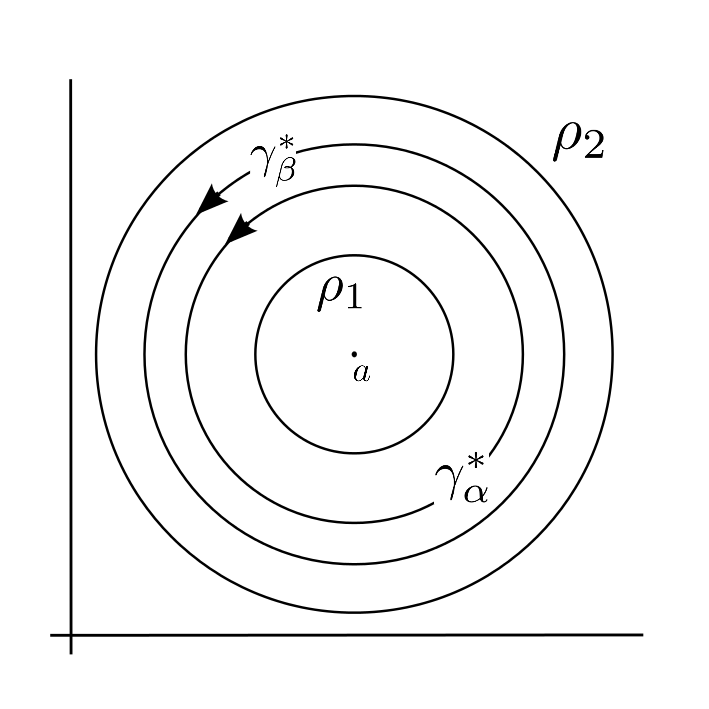
\includegraphics[width=0.3\textwidth]{39.png}
  \end{center}
\end{wrapfigure}

$\gamma_{\alpha}:t\in\left[  0,2\pi\right]  \longmapsto a+\alpha e^{it}\in\mathbb{C}$ 

e  $\gamma_{\beta}:t\in\left[  0,2\pi\right]  \longmapsto a+\beta e^{it}\in\mathbb{C}$

É claro que $\gamma_{\alpha}$ e $\gamma_{\beta}$ são $\Omega$-HCF

e então,pela Prop. 7.6, resulta

que $\gamma_{\alpha}\overset{\Omega}{\backsim}\gamma_{\beta},$ donde

\bigskip$\Gamma:=\gamma_{\beta}-\gamma_{\alpha}\overset{\Omega}{\backsim}0,$ o
que pelo

Teor. 7.1 implica\\

 \textsc{I}nd$_{\Gamma}(  z)  f(
z)  =\dfrac{1}{2\pi i}\underset{\Gamma}{%
%TCIMACRO{\dint }%
%BeginExpansion
{\displaystyle\int}
%EndExpansion
}\dfrac{f(  \lambda)  d\lambda}{\lambda-z}$ \ \ \ \ \ $\forall$
\ \ \ $\Omega$ $\backslash\gamma_{\alpha}^{\ast}\cup\gamma_{\beta}^{\ast}$

\bigskip

Se $z\in A\left[  a;\alpha,\beta\right]  $ então pela Prop. 5.3, tem-se

\ \ \ \ \ \ \ \ \ \ \ \ \ \ \textsc{I}nd$_{\Gamma}(  z)
=$\textsc{I}nd$_{\gamma_{\beta}}(  z)  -$\textsc{I}nd$_{\gamma
_{\alpha}}(  z)  =1-0=1$

portanto, a identidade acima se escreve na forma

\bigskip

$(  8.8.3)  $ \ \ \ \ \ \ $f(  z)  =\dfrac{1}{2\pi
i}\underset{\gamma_{\beta}}{%
%TCIMACRO{\dint }%
%BeginExpansion
{\displaystyle\int}
%EndExpansion
}\dfrac{f(  \lambda)  d\lambda}{\lambda-z}-\dfrac{1}{2\pi
i}\underset{\gamma_{\alpha}}{%
%TCIMACRO{\dint }%
%BeginExpansion
{\displaystyle\int}
%EndExpansion
}\dfrac{f(  \lambda)  d\lambda}{\lambda-z}$

$\forall$\ \ $z\in A\left[  a;\alpha,\beta\right]  $

\bigskip

O Teor. 4.3 mostra que a função

\ \ \ \ \ \ \ \ \ \ \ \ \ \ \ \ \ $z\in%
%TCIMACRO{\U{2102} }%
%BeginExpansion
\mathbb{C}
%EndExpansion
\backslash\gamma_{\beta}^{\ast}\longmapsto\dfrac{1}{2\pi i}\underset
{\gamma_{\beta}}{%
%TCIMACRO{\dint }%
%BeginExpansion
{\displaystyle\int}
%EndExpansion
}\dfrac{f(  \lambda)  d\lambda}{\lambda-z}\in%
%TCIMACRO{\U{2102} }%
%BeginExpansion
\mathbb{C}
%EndExpansion
$

é analítica e, em particular, a função

\ \ \ \ \ \ \ \ \ \ \ \ \ \ \ $f_{\beta}:z\in D_{\beta}(  a)
\longmapsto\dfrac{1}{2\pi i}\underset{\gamma_{\beta}}{%
%TCIMACRO{\dint }%
%BeginExpansion
{\displaystyle\int}
%EndExpansion
}\dfrac{f(  \lambda)  d\lambda}{\lambda-z}\in%
%TCIMACRO{\U{2102} }%
%BeginExpansion
\mathbb{C}
%EndExpansion
$

é analítica. De modo análogo, a função

\ \ \ \ \ \ \ \ \ \ \ \ \ \ $z\in%
%TCIMACRO{\U{2102} }%
%BeginExpansion
\mathbb{C}
%EndExpansion
\backslash\gamma_{\alpha}^{\ast}\longmapsto-\dfrac{1}{2\pi i}\underset
{\gamma_{\alpha}}{%
%TCIMACRO{\dint }%
%BeginExpansion
{\displaystyle\int}
%EndExpansion
}\dfrac{f(  \lambda)  d\lambda}{\lambda-z}\in%
%TCIMACRO{\U{2102} }%
%BeginExpansion
\mathbb{C}
%EndExpansion
$

é analítica e, em particular, a função

\ \ \ \ \ \ \ \ \ \ \ \ \ $f_{\alpha}:z\in%
%TCIMACRO{\U{2102} }%
%BeginExpansion
\mathbb{C}
%EndExpansion
\backslash\overline{D}_{\alpha}(  a)  \longmapsto-\dfrac{1}{2\pi
i}\underset{\gamma_{\alpha}}{%
%TCIMACRO{\dint }%
%BeginExpansion
{\displaystyle\int}
%EndExpansion
}\dfrac{f(  \lambda)  d\lambda}{\lambda-z}\in%
%TCIMACRO{\U{2102} }%
%BeginExpansion
\mathbb{C}
%EndExpansion
$

é analítica. Por $(  8.8.3)  $ podemos escrever

\bigskip

$(  8.8.4)  $ \ $\ \ \ \ \ \ \ \left\vert
\begin{array}
[c]{c}%
f(  z)  =f_{\beta}(  z)  +f_{\alpha}(  z)
\text{ \ \ }\forall\text{ \ \ }z\in A\left[  a;\alpha,\beta\right]  ,\text{
\ sempre que \ }\\
\text{ \ \ }\rho_{1}<\alpha<\beta<\rho_{2}.\text{
\ \ \ \ \ \ \ \ \ \ \ \ \ \ \ \ \ \ \ \ \ \ \ \ \ \ \ \ \ \ \ \ \ \ \ \ \ \ \ \ \ \ \ \ \ \ \ \ \ \ \ \ \ \ \ }%
\end{array}
\right.  $

\bigskip

A prova do Teor. 4.3 ( e a definição de integral de linha) mostram que o

desenvolvimento de Taylor de $f_{\beta}$ em volta de $a$ (válido em
$D_{\beta}(  a)  $ pelo

Corol. 4.11) é

\bigskip

$(  8.8.5)  $\ \ \ \ \ \ \ $\left\vert
\begin{array}
[c]{c}%
f_{\beta}(  z)  =\underset{m=0}{\overset{+\infty}{%
%TCIMACRO{\dsum }%
%BeginExpansion
{\displaystyle\sum}
%EndExpansion
}}\left\{  \dfrac{1}{2\pi i}\overset{}{\underset{\gamma_{\beta}}{%
%TCIMACRO{\dint }%
%BeginExpansion
{\displaystyle\int}
%EndExpansion
}}\dfrac{f(  \lambda)  d\lambda}{(  \lambda-a)  ^{m+1}%
}\right\}  (  z-a)  ^{m}\text{ \ \ }\forall\text{ \ \ }z\in
D_{\beta}(  a)  ,\text{ \ }\\
\text{\ \ \ \ \ \ \ \ \ \ \ \ \ \ \ \ \ \ \ \ \ \ \ \ \ \ \ \ \ \ \ \ \ \ \ \ \ \ \ \ \ \ \ \ \ \ \ \ \ \ \ \ \ \ \ \ \ }%
\\
\text{\ \ sempre que }\beta\in]\rho_{1,}\rho_{2}[.\text{
\ \ \ \ \ \ \ \ \ \ \ \ \ \ \ \ \ \ \ \ \ \ \ \ \ \ \ \ \ \ \ \ \ \ \ \ \ \ \ \ \ \ \ \ \ \ \ \ \ \ \ \ \ \ }%
\end{array}
\right.  $

\ \ \ \ \ \ \ \ \ \ \ 

Dado $r\in]\rho_{1},\rho_{2}[$ arbitrário, se $\gamma = \gamma_{r}:t\in\left[
0,2\pi\right]  \longmapsto a+re^{it}\in%
%TCIMACRO{\U{2102} }%
%BeginExpansion
\mathbb{C}
%EndExpansion
,$ é claro

 que $\gamma_{\beta}$ e $\gamma$ são $\Omega$-HCF e como

\bigskip

$(  8.8.6)  $ \ \ \ \ \ \ \ \ \ \ \ \ $(  z\in\Omega
\longmapsto\dfrac{f(  z)  }{(  z-a)  ^{m+1}}\in%
%TCIMACRO{\U{2102} }%
%BeginExpansion
\mathbb{C}
%EndExpansion
)  \in\mathcal{H}(  \Omega)  $ \ \ $\forall$ \ $m\in%
%TCIMACRO{\U{2124} }%
%BeginExpansion
\mathbb{Z}
%EndExpansion
$

\bigskip

pelo Teor. 7.7. (2%
%TCIMACRO{\U{ba}}%
%BeginExpansion
${{}^o}$%
%EndExpansion
), temos (usando $(  8.8.6)  $ \ \ $\forall$ \ $m\in%
%TCIMACRO{\U{2115} }%
%BeginExpansion
\mathbb{N}
%EndExpansion
$):

\bigskip\ \ \ \ \ \ \ \ \ \ \ \ \ \ \ \ \ \ \ \ \ \ \ $\underset{\gamma
_{\beta}}{\overset{}{%
%TCIMACRO{\dint }%
%BeginExpansion
{\displaystyle\int}
%EndExpansion
}}\dfrac{f(  \lambda)  d\lambda}{(  \lambda-a)  ^{m+1}%
}=\underset{\gamma}{%
%TCIMACRO{\dint }%
%BeginExpansion
{\displaystyle\int}
%EndExpansion
}\dfrac{f(  \lambda)  d\lambda}{(  \lambda-a)  ^{m+1}}$
\ \ \ $\forall$ \ \ $m\in%
%TCIMACRO{\U{2115} }%
%BeginExpansion
\mathbb{N}
%EndExpansion
$

o que mostra que $(  8.8.5)  $ se escreve assim

\bigskip

$(  8.8.5^{\prime})  $\ \ \ \ \ \ $\left\vert
\begin{array}
[c]{c}%
f_{\beta}(  z)  =\underset{m=0}{\overset{+\infty}{%
%TCIMACRO{\dsum }%
%BeginExpansion
{\displaystyle\sum}
%EndExpansion
}}\left\{  \dfrac{1}{2\pi i}\underset{\left\vert \lambda-a\right\vert =r}{%
%TCIMACRO{\dint }%
%BeginExpansion
{\displaystyle\int}
%EndExpansion
}\dfrac{f(  \lambda)  d\lambda}{(  \lambda-a)  ^{m+1}%
}\right\}  (  z-a)  ^{m}\text{ \ \ }\forall\text{ \ \ }z\in
D_{\beta}(  a) \\
\\
\text{quaisquer que sejam }r,\beta\in]\rho_{1},\rho_{2}[.\text{
\ \ \ \ \ \ \ \ \ \ \ \ \ \ \ \ \ \ \ \ \ \ \ \ \ \ \ \ \ \ \ \ \ \ \ \ \ \ \ \ \ \ }%
\end{array}
\right.  $

\bigskip

Em consequência, se definimos $f_{(  2)  }:=\underset{\rho
_{1}<\beta<\rho_{2}}{%
%TCIMACRO{\dbigcup }%
%BeginExpansion
{\displaystyle\bigcup}
%EndExpansion
}f_{\beta}$ \ é claro que $Dom(  f_{(  2)  })  =$

$=\underset{\rho_{1}<\beta<\rho_{2}}{%
%TCIMACRO{\dbigcup }%
%BeginExpansion
{\displaystyle\bigcup}
%EndExpansion
}D_{\beta}(  a)  =D_{\rho_{2}}(  a)  $ \ e então, em
vista de $(  8.8.5^{\prime})  $ tem-se:

\bigskip

$(  8.8.7)  $ \ \ $\left\vert
\begin{array}
[c]{c}%
f_{(  2)  }(  z)  =\underset{m=0}{\overset{+\infty}{%
%TCIMACRO{\dsum }%
%BeginExpansion
{\displaystyle\sum}
%EndExpansion
}}\left\{  \dfrac{1}{2\pi i}\underset{\left\vert \lambda-a\right\vert =r}{%
%TCIMACRO{\dint }%
%BeginExpansion
{\displaystyle\int}
%EndExpansion
}\dfrac{f(  \lambda)  d\lambda}{(  \lambda-a)  ^{m+1}%
}\right\}  (  z-a)  ^{m}\text{
\ \ para\ \ cada\ \ \ \ \ \ \ \ \ \ \ \ \ \ \ \ \ \ \ \ \ \ \ \ \ \ \ }\\
\text{\ }z\in D_{\rho_{2}}(  a)  ,\text{\ sendo a convergência
absoluta e uniforme em \ }\overline{D}_{s_{2}}(  a)
\text{\ \ \ \ \ \ \ \ \ \ \ \ \ \ \ \ \ \ \ \ \ \ }\\
\text{\ para cada \ \ }s_{2}\in\text{ }]0,\rho_{2}[.\text{
\ \ \ \ \ \ \ \ \ \ \ \ \ \ \ \ \ \ \ \ \ \ \ \ \ \ \ \ \ \ \ \ \ \ \ \ \ \ \ \ \ \ \ \ \ \ \ \ \ \ \ \ \ \ \ \ \ \ \ \ \ \ \ \ \ \ \ \ \ \ \ \ \ \ \ \ \ \ \ }%
\end{array}
\right.  $

\bigskip

Por outro lado, $\forall$ $\ \lambda\in\gamma_{\alpha}^{\ast}$ \ (i.e.
$\left\vert \lambda-a\right\vert =\alpha$) \ e $\forall$ \ $z\in%
%TCIMACRO{\U{2102} }%
%BeginExpansion
\mathbb{C}
%EndExpansion
\backslash\overline{D}_{\alpha}(  a)  $ \ (isto é

$\left\vert z-a\right\vert >\alpha$) temos $\ \left\vert \dfrac{\lambda
-a}{z-a}\right\vert <1,$ donde

$\dfrac{1}{\lambda-z}=-\dfrac{1}{z-a}(  \dfrac{1}{1-\dfrac{\lambda
-a}{z-a}})  =-\dfrac{1}{z-a}\underset{n\geq0}{%
%TCIMACRO{\dsum }%
%BeginExpansion
{\displaystyle\sum}
%EndExpansion
}(  \dfrac{\lambda-a}{z-a})  ^{n}=-\underset{n\geq0}{%
%TCIMACRO{\dsum }%
%BeginExpansion
{\displaystyle\sum}
%EndExpansion
}\dfrac{(  \lambda-a)  ^{n}}{(  z-a)  ^{n+1}}.$

\bigskip

Observemos que $\forall$ \ $z\in%
%TCIMACRO{\U{2102} }%
%BeginExpansion
\mathbb{C}
%EndExpansion
\backslash\overline{D}_{\alpha}(  a)  $ fixado, temos

\bigskip\ \ \ \ \ \ \ \ \ \ \ \ \ \ \ \ $\underset{\lambda\in\gamma_{\alpha
}^{\ast}}{\sup}\left\vert \dfrac{(  \lambda-a)  ^{n}}{(
z-a)  ^{n+1}}\right\vert =\dfrac{1}{\alpha}(  \dfrac{\alpha
}{\left\vert z-a\right\vert })  ^{n+1}$ \ \ \ \ \ $(  n\in%
%TCIMACRO{\U{2115} }%
%BeginExpansion
\mathbb{N}
%EndExpansion
)  $

e como a série numérica ($z$ é fixo!) $\underset{n\geq0}{%
%TCIMACRO{\dsum }%
%BeginExpansion
{\displaystyle\sum}
%EndExpansion
}\dfrac{1}{\alpha}(  \dfrac{\alpha}{z-a})  ^{n+1}$ \ é absolutamente

convergente, pela Prop. 3.5 (teste M de Weierstras) resulta que a

série

\ \ \ \ \ \ \ \ \ \ \ \ \ \ \ \ \ \ \ \ \ \ \ \ \ \ \ \ \ \ \ \ \ \ $-\underset
{n\geq0}{%
%TCIMACRO{\dsum }%
%BeginExpansion
{\displaystyle\sum}
%EndExpansion
}\dfrac{(  \lambda-a)  ^{n}}{(  z-a)  ^{n+1}}$

é absolutamente convergente $\forall$ \ \ $\lambda\in\gamma_{\alpha}%
^{\ast}$ \ e \ $\forall$ \ $z\in%
%TCIMACRO{\U{2102} }%
%BeginExpansion
\mathbb{C}
%EndExpansion
\backslash\overline{D}_{\alpha}(  a)  $ e, além disso,

é uniformemente convergente em $\lambda\in\gamma_{\alpha}^{\ast},$
\ $\forall$ \ $z\in%
%TCIMACRO{\U{2102} }%
%BeginExpansion
\mathbb{C}
%EndExpansion
\backslash\overline{D}_{\alpha}(  a)  .$ Como $f$ \ é

contínua e portanto limitada sobre o compacto $\gamma_{\alpha}^{\ast},$
resulta que a série

(ver exerc. 4.2)

\ \ \ \ \ \ \ \ \ \ \ \ \ \ \ \ \ \ \ \ \ \ \ \ \ $\dfrac{f(
\lambda)  }{\lambda-z}=-\underset{n\geq0}{%
%TCIMACRO{\dsum }%
%BeginExpansion
{\displaystyle\sum}
%EndExpansion
}\dfrac{f(  \lambda)  (  \lambda-a)  ^{n}}{(
z-a)  ^{n+1}}$

é absolutamente convergente $\forall$ \ $\lambda\in\gamma_{\alpha}^{\ast
},$ \ $\forall$ \ $z\in%
%TCIMACRO{\U{2102} }%
%BeginExpansion
\mathbb{C}
%EndExpansion
\backslash\overline{D}_{\alpha}(  a)  $ e, uniforme--

mente convergente em $\lambda\in\gamma_{\alpha}^{\ast}$ , \ $\forall$ \ $z\in%
%TCIMACRO{\U{2102} }%
%BeginExpansion
\mathbb{C}
%EndExpansion
\backslash\overline{D}_{\alpha}(  a)  $ fixado. Em consequência

podemos integrar termo a termo em relação a $\lambda,$ obtendo
$\ \forall$ \ $z\in%
%TCIMACRO{\U{2102} }%
%BeginExpansion
\mathbb{C}
%EndExpansion
\backslash\overline{D}_{\alpha}(  a)  :$

\bigskip$\underset{\gamma_{\alpha}}{%
%TCIMACRO{\dint }%
%BeginExpansion
{\displaystyle\int}
%EndExpansion
}\dfrac{f(  \lambda)  d\lambda}{\lambda-z}=-\underset{n\geq0}{%
%TCIMACRO{\dsum }%
%BeginExpansion
{\displaystyle\sum}
%EndExpansion
\text{ }}\underset{\gamma_{\alpha}}{%
%TCIMACRO{\dint }%
%BeginExpansion
{\displaystyle\int}
%EndExpansion
}\dfrac{f(  \lambda)  (  \lambda-a)  ^{n}}{(
z-a)  ^{n+1}}d\lambda=-\underset{n\geq0}{%
%TCIMACRO{\dsum }%
%BeginExpansion
{\displaystyle\sum}
%EndExpansion
}\left\{  \underset{\gamma_{\alpha}}{%
%TCIMACRO{\dint }%
%BeginExpansion
{\displaystyle\int}
%EndExpansion
}\dfrac{f(  \lambda)  d\lambda}{(  \lambda-a)  ^{-n}%
}\right\}  \dfrac{1}{(  z-a)  ^{n+1}}=$

$=-\underset{k=-1}{\overset{-\infty}{%
%TCIMACRO{\dsum }%
%BeginExpansion
{\displaystyle\sum}
%EndExpansion
}}\left\{  \underset{\gamma_{\alpha}}{%
%TCIMACRO{\dint }%
%BeginExpansion
{\displaystyle\int}
%EndExpansion
}\dfrac{f(  \lambda)  d\lambda}{(  \lambda-a)  ^{k+1}%
}\right\}  (  z-a)  ^{k},$ donde ( ver definição de
$f_{\alpha}$)

\bigskip

$(  8.8.8)  $ \ \ $\left\vert
\begin{array}
[c]{c}%
f_{\alpha}(  z)  =\underset{m=-1}{\overset{-\infty}{%
%TCIMACRO{\dsum }%
%BeginExpansion
{\displaystyle\sum}
%EndExpansion
}}\left\{ \frac{1}{2\pi i}  \underset{\gamma_{\alpha}}{%
%TCIMACRO{\dint }%
%BeginExpansion
{\displaystyle\int}
%EndExpansion
}\dfrac{f(  \lambda)  d\lambda}{(  \lambda-a)  ^{m+1}%
}\right\}  (  z-a)  ^{m}\text{ \ \ }\forall\text{ \ }z\in%
%TCIMACRO{\U{2102} }%
%BeginExpansion
\mathbb{C}
%EndExpansion
\backslash\overline{D}_{\alpha}(  a)  ,\\
\text{sempre que }\alpha\in]\rho_{1},\rho_{2}\lbrack.
\text{\ \ \ \ \ \ \ \ \ \ \ \ \ \ \ \ \ \ \ \ \ \ \ \ \ \ \ \ \ \ \ \ \ \ \ \ \ \ \ \ \ \ \ \ \ \ \ \ \ \ \ \ \ }%
\end{array}
\right.  $

\bigskip

Se $s_{1}>\alpha$ então $F:=%
%TCIMACRO{\U{2102} }%
%BeginExpansion
\mathbb{C}
%EndExpansion
\backslash D_{s_{1}}(  a)  $ é um fechado contido no aberto

$A:=%
%TCIMACRO{\U{2102} }%
%BeginExpansion
\mathbb{C}
%EndExpansion
\backslash\overline{D}_{\alpha}(  a)  ;$ vamos mostrar que a
série em $(  8.8.7)  $ é absoluta e

uniformemente convergente em $F.$ De fato, fixemos $\sigma$ tal que

$\rho_{1}<\sigma<s_{1}$ e $\sigma<\rho_{2\text{ }}$ e seja

\ \ \ \ \ \ \ \ \ \ \ \ \ \ \ \ \ \ \ \ \ \ \ \ $\gamma_{\sigma}:t\in\left[
0,2\pi\right]  \longmapsto a+\sigma e^{it}\in%
%TCIMACRO{\U{2102} }%
%BeginExpansion
\mathbb{C}.
%EndExpansion
$

Então, $\gamma_{\sigma}$ e $\gamma_{\alpha}$ são $\Omega$-HCF e
$(  8.8.6)  $ mostra que em $(  8.8.8)  $ podemos

substituir $\gamma_{\alpha}$ por $\gamma_{\sigma},$ majorando o módulo do
termo geral da série em

$(  8.8.8)  $ assim $[z\in F$ e $m\in%
%TCIMACRO{\U{2124} }%
%BeginExpansion
\mathbb{Z}
%EndExpansion
_{-}^{\ast}!]:$

\bigskip

$\ \ \ \ \ \ \ \ \ \ \ \left\vert \dfrac{1}{2\pi i}\underset{\gamma_{\alpha}}{%
%TCIMACRO{\dint }%
%BeginExpansion
{\displaystyle\int}
%EndExpansion
}\dfrac{f(  \lambda)  d\lambda}{(  \lambda-a)  ^{m+1}%
}(  z-a)  ^{m}\right\vert =\dfrac{1}{2\pi}\left\vert \underset
{\gamma_{\sigma}}{%
%TCIMACRO{\dint }%
%BeginExpansion
{\displaystyle\int}
%EndExpansion
}\dfrac{f(  \lambda)  d\lambda}{(  \lambda-a)  ^{m+1}%
}(  z-a)  ^{m}\right\vert \overset{(  \ast)  }{\leq}$

\bigskip

$\overset{(  \ast)  }{\leq}\dfrac{1}{2\pi}\underset{\gamma_{\sigma
}}{%
%TCIMACRO{\dint }%
%BeginExpansion
{\displaystyle\int}
%EndExpansion
}\dfrac{\left\vert f(  \lambda)  \right\vert \left\vert
d\lambda\right\vert }{\sigma^{m+1}}s_{1}^{m}\leq\left\Vert f\right\Vert
_{\gamma_{\sigma}^{\ast}}\cdot(  \dfrac{s_{1}}{\sigma})  ^{m},$
onde $(  \ast)  $ resulta observando que

$z\in F\iff\left\vert z-a\right\vert \geq s_{1}$ e portanto $\left\vert
z-a\right\vert ^{m}\leq s_{1}^{m}$ \ $\forall$ \ $m\in%
%TCIMACRO{\U{2124} }%
%BeginExpansion
\mathbb{Z}
%EndExpansion
_{-}^{\ast}.$ Em

consequência, definindo $c:=\left\Vert f\right\Vert _{\gamma_{\sigma
}^{\ast}}$ \ resulta

\ \ \ \ \ \ \ \ \ \ \ \ \ $\underset{z\in F}{\sup}\left\vert \dfrac{1}{2\pi
i}\underset{\gamma_{\alpha}}{%
%TCIMACRO{\dint }%
%BeginExpansion
{\displaystyle\int}
%EndExpansion
}\dfrac{f(  \lambda)  d\lambda}{(  \lambda-a)  ^{m+1}%
}(  z-a)  ^{m}\right\vert \leq c(  \dfrac{\sigma}{s_{1}%
})  ^{-m}$ \ \ $\forall$ \ $m\in%
%TCIMACRO{\U{2124} }%
%BeginExpansion
\mathbb{Z}
%EndExpansion
_{-}^{\ast}$

e como a série

\ \ \ \ \ \ \ \ \ \ \ \ \ \ \ \ \ \ \ \ \ \ \ \ \ \ \ \ $\underset
{m=-1}{\overset{-\infty}{%
%TCIMACRO{\dsum }%
%BeginExpansion
{\displaystyle\sum}
%EndExpansion
}}(  \dfrac{\sigma}{s_{1}})  ^{-m}=\overset{+\infty}{\underset
{p=1}{%
%TCIMACRO{\dsum }%
%BeginExpansion
{\displaystyle\sum}
%EndExpansion
}}(  \dfrac{\sigma}{s_{1}})  ^{p}$

é convergente (pois $\sigma<s_{1}$), de novo pela Prop. 3.5, resulta que a
série em

$(  8.8.8)  $ é absoluta e uniformemente convergente em $F.$
Como $\gamma_{\alpha}$ e $\gamma$ \ são

$\Omega$-HCF, por $(  8.8.8)  $ podemos substituir $\gamma_{\alpha
}$ por $\gamma$ ( de novo pelo Teor. 7.7

(2%
%TCIMACRO{\U{ba}}%
%BeginExpansion
${{}^o}$%
%EndExpansion
)), logo $(  8.8.8)  $ se escreve assim:

\ \ \ \ \ \ \ $\left\vert
\begin{array}
[c]{c}%
f_{\alpha}(  z)  =\underset{m=-1}{\overset{-\infty}{%
%TCIMACRO{\dsum }%
%BeginExpansion
{\displaystyle\sum}
%EndExpansion
}}\left\{  \dfrac{1}{2\pi i}\underset{\gamma}{%
%TCIMACRO{\dint }%
%BeginExpansion
{\displaystyle\int}
%EndExpansion
}\dfrac{f(  \lambda)  d\lambda}{(  \lambda-a)  ^{m+1}%
}\right\}  (  z-a)  ^{m}\text{ \ \ }\forall\text{ \ }z\in%
%TCIMACRO{\U{2102} }%
%BeginExpansion
\mathbb{C}
%EndExpansion
\backslash\overline{D}_{\alpha}(a)\text{ \ \ \ \ \ \ \ \ \ \ \ \ \ \ \ \ \ \ }\\
\text{\ e \ }\forall\text{ \ }r,\alpha\in]\rho_{1},\rho_{2[\text{ }.\text{
\ \ \ \ \ \ \ \ \ \ \ \ \ \ \ \ \ \ \ \ \ \ \ \ \ \ \ \ \ \ \ \ \ \ \ \ \ \ \ \ \ \ \ \ \ \ \ \ \ \ \ \ \ \ \ \ \ \ \ \ \ \ \ \ \ \ \ \ \ \ \ \ \ \ \ \ \ \ \ \ \ \ \ \ \ \ \ \ \ \ \ }%
}%
\end{array}
\right.  $

\bigskip

Em consequência, definindo $f_{(  1)  }:=\underset{\rho
_{1}<\alpha<\rho_{2}}{%
%TCIMACRO{\dbigcup }%
%BeginExpansion
{\displaystyle\bigcup}
%EndExpansion
}f_{\alpha}$ $,$ é claro que $Dom(  f_{(  1)  })  =$

$=\underset{\rho_{1}<\alpha<\rho_{2}}{%
%TCIMACRO{\dbigcup }%
%BeginExpansion
{\displaystyle\bigcup}
%EndExpansion
}(
%TCIMACRO{\U{2102} }%
%BeginExpansion
\mathbb{C}
%EndExpansion
\backslash\overline{D}_{\alpha}(  a)  )  =%
%TCIMACRO{\U{2102} }%
%BeginExpansion
\mathbb{C}
%EndExpansion
\backslash\overline{D}\rho_{1}(  a)  $ e, em vista das propriedades
de conver-

gência da série em $(  8.8.8)  $ já verificadas, resulta

\bigskip

$(  8.8.9)  \left\vert
\begin{array}
[c]{c}%
f_{(  1)  }(  z)  =\underset{m=-1}{\overset{-\infty}{%
%TCIMACRO{\dsum }%
%BeginExpansion
{\displaystyle\sum}
%EndExpansion
}}\left\{  \dfrac{1}{2\pi i}\underset{\left\vert \lambda-a\right\vert =r}{%
%TCIMACRO{\dint }%
%BeginExpansion
{\displaystyle\int}
%EndExpansion
}\dfrac{f(  \lambda)  d\lambda}{(  \lambda-a)  ^{m+1}%
}\right\}  (  z-a)  ^{m}\text{ \ }\forall\text{ \ }z\in%
%TCIMACRO{\U{2102} }%
%BeginExpansion
\mathbb{C}
%EndExpansion
\backslash\overline{D}_{\rho_{1}}(  a)  \text{\ \ \ \ }\\
\text{ \ \ \ \ \ }\\
\text{\ e \ }\forall\text{ \ }r\in]\rho_{1},\rho_{2}[,\text{ sendo a
convergência absoluta e uniforme \ \ \ \ \ \ \ \ \ \ \ \ \ \ }\\
\text{em }%
%TCIMACRO{\U{2102} }%
%BeginExpansion
\mathbb{C}
%EndExpansion
\backslash D_{s_{1}}(  a)  \text{ sempre que }s_{1}>\rho_{1}.\text{
\ \ \ \ \ \ \ \ \ \ \ \ \ \ \ \ \ \ \ \ \ \ \ \ \ \ \ \ \ \ \ \ \ \ \ \ \ \ \ \ \ \ \ \ }%
\end{array}
\right.  $

\bigskip

Observando finalmente que das definições de $f_{(  2)  }$ e
de $f_{(  1)  }$ e de $(  8.8.4)  $

resulta

\ \ \ \ \ \ \ \ \ \ \ \ \ \ $f(  z)  =f_{(  2)  }(
z)  +f_{(  1)  }(  z)  $ \ \ $\forall$
\ $z\in\Omega=A\left[  a;\rho_{1},\rho_{2}\right]  $

o que junto com $(  8.8.7)  ,$ $(  8.8.8)  $ e a Def.
8.7, implica

\ \ \ \ \ $f(  z)  =\underset{m=-\infty}{\overset{+\infty}{%
%TCIMACRO{\dsum }%
%BeginExpansion
{\displaystyle\sum}
%EndExpansion
}}\left\{  \dfrac{1}{2\pi i}\underset{\left\vert \lambda-a\right\vert =r}{%
%TCIMACRO{\dint }%
%BeginExpansion
{\displaystyle\int}
%EndExpansion
}\dfrac{f(  \lambda)  d\lambda}{(  \lambda-a)  ^{m+1}%
}\right\}  (  z-a)  ^{m}$ \ \ $\forall$ \ $z\in A\left[  a;\rho
_{1},\rho_{2}\right]  $ \ \ 

e $\forall$ \ $r\in]\rho_{1},\rho_{2}[,$ sendo \textit{a convergência
}absoluta e uniforme no anel compac-

\bigskip

to $\overline{A\left[  a;s_{1},s_{2}\right]  }$ \ \ $(  \rho_{1}%
<s_{1}<s_{2}<\rho_{2})  \cdot$ \ $\square$

\bigskip

\textbf{Definição 8.9} \ Se $a\in%
%TCIMACRO{\U{2102} }%
%BeginExpansion
\mathbb{C}
%EndExpansion
,$ $0\leq\rho_{1}<\rho_{2}\leq+\infty$ \ e \ $f\in\mathcal{H}(  A\left[
a,\rho_{1},\rho_{2}\right]  )  $, a série

de $(  8.8.1)  $ é chamada \textit{desenvolvimento de Laurent
}(ou \textit{série de Laurent})

\textit{de} $f$ \textit{no anel }$A\left[  a,\rho_{1},\rho_{2}\right]  .$

\bigskip

Consideremos uma função analítica $f$ com uma singularidade
isolada num

ponto $a$, isto é,

\ \ \ \ \ \ \ \ \ \ \ \ \ \ \ \ \ \ \ \ \ \ \ \ \ $f\in\mathcal{H}(
A\left[  a,0,R\right]  )  $ , para algum $R>0$

Se $a$ não é removível o desenvolvimento de Laurent no anel
$A\left[  a,0,R\right]  $

substitui o desenvolvimento de Taylor de $f$ em volta de $a$ (que $\nexists$
pois a não

é removível) \ e a "parte negativa" do mesmo significa a forma em que deve

ser "corrigido o desenvolvimento de Taylor" para levar em consideração a

singularidade não removível em $a.$ Observemos ainda que em virtude do

Corol. 5.10 a "parte não negativa" do desenvolvimento de Laurent é formal-

mente idêntica ao desenvolvimento de Taylor. Estas considerações terão

um significado preciso no Corol. 8.10.

\bigskip

\textbf{Corolário 8.10 \ }\textit{Sejam }$\Omega$ \textit{um aberto de }$%
%TCIMACRO{\U{2102} }%
%BeginExpansion
\mathbb{C}
%EndExpansion
,$ $a\in\Omega,$ $f\in\mathcal{H}(  \Omega\backslash\left\{  a\right\}
)  ,$ $\rho>0$

\textit{tal que }$D_{\rho}^{*}(  a)  =A\left[  a,0,\rho
\right]  \subset\Omega\backslash\left\{  a\right\}  $ \textit{e}

\bigskip

$(  8.10.1)  $ \ \ \ \ \ \ \ \ \ \ \ \ \ \ \ \ $f(  z)
=\underset{m=-\infty}{\overset{\infty}{%
%TCIMACRO{\dsum }%
%BeginExpansion
{\displaystyle\sum}
%EndExpansion
}}a_{m}(  z-a)  ^{m}$ \ \ $\forall$ \ $z\in A\left[  a,0,\rho
\right]  $

\textit{a série de Laurent de }$f$ \textit{no anel }$A\left[
a,0,\rho\right]  .$ \textit{Então:}

(1%
%TCIMACRO{\U{ba}}%
%BeginExpansion
${{}^o}$%
%EndExpansion
) \ \textit{O ponto }$a$ \textit{é uma singularidade removível de
}$f$ \textit{se e só se }$a_{m}=0$ \ 

$\forall$ \ $m\in%
%TCIMACRO{\U{2124} }%
%BeginExpansion
\mathbb{Z}
%EndExpansion
_{-}^{\ast}.$

(2%
%TCIMACRO{\U{ba}}%
%BeginExpansion
${{}^o}$%
%EndExpansion
) \ \textit{O ponto }$a$ \textit{é um polo de ordem }$\nu$ ($>0,$ por
definição) \textit{de }$f$ \textit{se e só }

\textit{se }$a_{\nu}\neq0$ \textit{e }$a_{m}=0$ \ $\forall$ \ $m\leq-\nu-1$

(3%
%TCIMACRO{\U{ba}}%
%BeginExpansion
${{}^o}$%
%EndExpansion
) \ \textit{O ponto }$a$ \textit{é uma singularidade essencial de }$f$
\textit{se e só se o conjunto}

\ \ \ \ \ \ \ \ \ \ \ \ \ \ \ \ \ \ \ \ \ \ \ \ \ \ \ \ \ \ \ \ $X=\left\{
m\in%
%TCIMACRO{\U{2124} }%
%BeginExpansion
\mathbb{Z}
%EndExpansion
_{-}^{\ast}\text{ }|\text{ }a_{m}\neq0\right\}  $

\textit{é infinito.}

\bigskip

\textbf{Prova \ }(1%
%TCIMACRO{\U{ba}}%
%BeginExpansion
${{}^o}$%
%EndExpansion
) \ Se o ponto $a$ é uma singularidade removível de $f$ então existe

$\varphi\in\mathcal{H}(  \Omega)  $ tal que

\bigskip

$(  8.10.2)  $ \ \ \ \ \ \ \ \ \ $f(  z)  =\varphi
(  z)  $ \ \ $\forall$ \ $z\in A\left[  a,0,\rho\right]  $
\ \ \ \ \ \ \ \ $(  z\in\Omega)  $

\bigskip

Seja

\bigskip

$(  8.10.3)  $ \ \ \ \ \ \ \ \ \ \ $\varphi(  z)
=\overset{\infty}{\underset{m=0}{%
%TCIMACRO{\dsum }%
%BeginExpansion
{\displaystyle\sum}
%EndExpansion
}}b_{m}(  z-a)  ^{m}$ \ \ $\forall$ \ $z\in D_{\rho}(
a)  $

\bigskip

a série de Taylor de $\varphi$ em volta de $a,$ então substituindo em
$(  8.10.2)  $

obtemos

\ \ \ \ \ \ \ \ \ \ \ \ \ \ \ \ \ \ $f(  z)  =\underset
{m=0}{\overset{\infty}{%
%TCIMACRO{\dsum }%
%BeginExpansion
{\displaystyle\sum}
%EndExpansion
}}b_{m}(  z-a)  ^{m}$ \ \ $\forall$ \ \ $z\in A\left[
a,0,\rho\right]  ,$

o que implica, por $8.10.1)$ e pela unicidade da série de Laurent, que

$a_{m}=b_{m}$ \ $\forall$ \ $m\in%
%TCIMACRO{\U{2115} }%
%BeginExpansion
\mathbb{N}
%EndExpansion
$ e $a_{m}=0$ \ \ $\forall$ \ $m\in%
%TCIMACRO{\U{2124} }%
%BeginExpansion
\mathbb{Z}
%EndExpansion
_{-}^{\ast}.$ Reciprocamente, se $a_{m}=0$

$\forall$ \ $m\in%
%TCIMACRO{\U{2124} }%
%BeginExpansion
\mathbb{Z}
%EndExpansion
_{-}^{\ast},$ então por $(  8.10.1)  $ temos

\bigskip

$(  8.10.4)  $ \ \ \ \ \ $f(  z)  =\overset{\infty
}{\underset{m=0}{%
%TCIMACRO{\dsum }%
%BeginExpansion
{\displaystyle\sum}
%EndExpansion
}}a_{m}(  z-a)  ^{m}$ \ \ $\forall$ \ \ $z\in A\left[
a,0,\rho\right]  $

\bigskip

e como o segundo membro de $(  8.10.4)  $ define uma função
analítica $\varphi$ em

$D_{\rho}(  a)  $ (ver exerc. 5.10), podemos escrever (por $(
8.10.4)  :$

\ \ \ \ \ \ \ \ \ \ \ \ \ \ $\varphi\in\mathcal{H}(  D_{\rho}(
a)  )  $ \ \ \ \ e \ \ \ \ $f(  z)  =\varphi(
z)  $ \ \ \ $\forall$ \ \ $z\in D_{\rho}^{*}(  a)  ,$

o que mostra que $a$ é uma singularidade removível de $f.$

(2%
%TCIMACRO{\U{ba}}%
%BeginExpansion
${{}^o}$%
%EndExpansion
) \ Se $a$ é um polo de ordem $\nu$ de $f,$ por definição existe
uma sequência

$(  c_{-k})  _{1\leq k\leq\nu}$ de números complexos com
$c_{-\nu}\neq0$ e existe $\varphi\in\mathcal{H}(  \Omega)  $ tal que

\bigskip

$(  8.10.5)  $ \ \ \ \ \ \ \ \ \ \ \ \ $f(  z)
-\underset{k=1}{\overset{\nu}{%
%TCIMACRO{\dsum }%
%BeginExpansion
{\displaystyle\sum}
%EndExpansion
}}\dfrac{c_{-k}}{(  z-a)  ^{k}}=\varphi(  z)  $
\ \ \ \ $\forall$ \ \ $z\in A\left[  a,0,\rho\right]  $ $.$

\bigskip

Se usamos de novo $(  8.10.3)  $ para indicar a série de Taylor
de $\varphi$ em

volta de $a$ (esta $\varphi$ não tem nada a ver com a $\varphi$ de (1%
%TCIMACRO{\U{ba}}%
%BeginExpansion
${{}^o}$%
%EndExpansion
) mas aqui inte-

ressa apenas a notação), por $(  8.10.5)  $ resulta

\bigskip

$(  8.10.6)  $ \ \ $f(  z)  =-\overset{\nu}%
{\underset{k=1}{%
%TCIMACRO{\dsum }%
%BeginExpansion
{\displaystyle\sum}
%EndExpansion
}}\dfrac{c_{-k}}{(  z-a)  ^{k}}=\underset{m=0}{\overset{\infty}{%
%TCIMACRO{\dsum }%
%BeginExpansion
{\displaystyle\sum}
%EndExpansion
}}b_{m}(  z-a)  ^{m}$ \ \ $\forall$ \ $z\in A\left[  a,0,\rho
\right]  $

\bigskip

o que pela unicidade da série de Laurent mostra que

\bigskip

$(  8.10.7)  $ \ \ \ \ \ $f(  z)  =\overset{\nu
}{\underset{k=1}{%
%TCIMACRO{\dsum }%
%BeginExpansion
{\displaystyle\sum}
%EndExpansion
}}\dfrac{c_{-k}}{(  z-a)  ^{k}}+\underset{m=0}{\overset{\infty}{%
%TCIMACRO{\dsum }%
%BeginExpansion
{\displaystyle\sum}
%EndExpansion
}}b_{m}(  z-a)  ^{m}$ \ \ $\forall$ \ \ $z\in A\left[
a,0,\rho\right]  $

\bigskip

é a série de Laurent de $f$ no anel $A\left[  a,0,\rho\right]  $, logo
por $(  8.10.1)  $ resulta

$a_{m}=b_{m}$ \ \ $\forall$ \ $m\in%
%TCIMACRO{\U{2115} }%
%BeginExpansion
\mathbb{N}
%EndExpansion
,$ $a_{-k}=c_{-k}$ \ \ $\forall$ \ $k=1,2,\ldots$ $,\nu$ \ donde, em particular,

$a_{-\nu}=c_{-\nu}\neq0$ e $a_{m}=0$ \ \ $\forall$ \ $m\leq-\nu-1.$%
Reciprocamente, suponhamos

que $\ a_{-\nu}\neq0$ e $a_{m}=0$ \ \ $\forall$ \ $m\leq-\nu-1$ então
é válida $(  8.10.7)  $ e portanto

$(  8.10.6)  $ com $a_{m}=b_{m}$ \ \ $\forall$ \ $m\in%
%TCIMACRO{\U{2115} }%
%BeginExpansion
\mathbb{N}
%EndExpansion
$ e que $a_{-k}=c_{-k}$ \ \ $\forall$ \ $k=1,2,$ $\ldots,$ $\nu.$

Ora, o segundo membro de $(  8.10.6)  $ \ (com $b_{m}=a_{m}$
\ \ $\forall$ \ $m\in%
%TCIMACRO{\U{2115} }%
%BeginExpansion
\mathbb{N}
%EndExpansion
$) define

uma função analítica $\psi$ em $D_{\rho}(  a)  $
\ (exerc. 5.10), logo podemos escrever

(por $(  8.10.6)  $):

\ \ \ \ \ \ \ \ \ $\psi\in\mathcal{H}(  D_{\rho}(  0)
)  $ \ \ e \ \ $f(  z)  -\overset{\nu}{\underset{k=1}{%
%TCIMACRO{\dsum }%
%BeginExpansion
{\displaystyle\sum}
%EndExpansion
}}\dfrac{a_{-k}}{(  z-a)  ^{k}}=\psi(  z)  $
\ \ $\forall$ \ $z\in D_{\rho}(  a)  $

o que significa precisamente que vale a condição (b) do Teor. 8.3, isto

é, \ $f$ tem um polo de ordem $\nu$ no ponto $(  a)  .$

(3%
%TCIMACRO{\U{ba}}%
%BeginExpansion
${{}^o}$%
%EndExpansion
) \ Se $a$ é uma singularidade essencial de $f$ e se o conjunto $X$ fosse fi-

nito, então por (1%
%TCIMACRO{\U{ba}}%
%BeginExpansion
${{}^o}$%
%EndExpansion
) e (2%
%TCIMACRO{\U{ba}}%
%BeginExpansion
${{}^o}$%
%EndExpansion
) \ $a$ seria uma singularidade removível ou polar

dependendo que $X=\varnothing$ ou $X\neq\varnothing$ respectivamente, o que
é absurdo,

logo $X$ é infinito. Reciprocamente, se $X$ é infinito então (1%
%TCIMACRO{\U{ba}}%
%BeginExpansion
${{}^o}$%
%EndExpansion
) e (2%
%TCIMACRO{\U{ba}}%
%BeginExpansion
${{}^o}$%
%EndExpansion
) mostram

que a singularidade em $a$ não pode ser nem removível nem polar, logo é

essencial. \ $\square$

\bigskip

A seguir vamos introduzir um conceito fundamental na teoria das funções

complexas de variável complexa que é o de \textit{função
meromorfa.} Se $\Omega$ é

um aberto conexo de $%
%TCIMACRO{\U{2102} }%
%BeginExpansion
\mathbb{C}
%EndExpansion
,$ $f,g\in\mathcal{H}(  \Omega)  $ e $g\neq0,$ sabemos pelo Corol. 4.16

que $D=Z(  g)  $ é um conjunto discreto e fechado em $\Omega$
(ou equivalentemente

$D$ não tem ponto de acumulação em $\Omega,$ ver exerc. (4.11)
(c)), em consequên-

cia $\Omega\backslash D$ é aberto em $%
%TCIMACRO{\U{2102} }%
%BeginExpansion
\mathbb{C}
%EndExpansion
$ e pelo Exemplo 3 do capítulo 1 é claro que

\ \ \ \ \ \ \ \ \ \ \ \ \ \ \ \ \ \ \ \ \ \ \ \ \ \ \ \ \ \ \ \ \ \ \ \ \ \ \ $f/g\in
\mathcal{H}(  \Omega\backslash D)  $.

Se $a\in D$ (e $f\neq0$), sabemos que existem $\nu,\mu\in%
%TCIMACRO{\U{2115} }%
%BeginExpansion
\mathbb{N}
%EndExpansion
$ \ $\nu\geq1$, $\mu\geq0$ \ e

$D_{r}(  a)  \subset\Omega$ tais que

$\ \ \ \ \ \ \ \ \ \ \ \ \ \ \ \ \ g(  z)  =(  z-a)
^{\nu}g_{1}(  z)  $ \ \ \ \ e \ \ \ \ $f(  z)  =(
z-a)  ^{\mu}\cdot f_{1}(  z)  ,$

onde $f_{1},g_{1}\in\mathcal{H}(  D_{r}(  a)  )  ,$
$f_{1}(  z)  \neq0$ e $g_{1}(  z)  \neq0$ para cada
$z\in D_{r}(  a)  .$

Resulta que

\ \ \ \ \ \ \ \ \ \ \ \ \ \ \ \ $f_{1}/g_{1}\in\mathcal{H}(  D_{r}(
a)  )  $\ $\ \ \ \ \ $e \ \ \ \ \ $(  f_{1}/g_{1})
(  z)  \neq0$ \ \ $\forall$ \ \ $z\in D_{r}(  a)  $\ \ 

logo

\ \ \ \ \ \ \ \ \ \ \ \ \ \ \ $\dfrac{f_{1}(  z)  }{g_{1}(
z)  }=\underset{m\geq0}{%
%TCIMACRO{\dsum }%
%BeginExpansion
{\displaystyle\sum}
%EndExpansion
}$\ $c_{m}(  z-a)  ^{m}$\ \ \ \ \ \ $\forall$ \ \ $z\in
D_{r}(  a)  $\ \ \ e \ \ \ $c_{0}\neq0$

donde

\ \ \ \ 

$\dfrac{f(  z)  }{g(  z)  }=\dfrac{(  z-a)
^{\mu}}{(  z-a)  ^{\nu}}\cdot\dfrac{f_{1}(  z)  }%
{g_{1}(  z)  }=(  z-a)  ^{\mu-\nu}\cdot\underset{m\geq
0}{%
%TCIMACRO{\dsum }%
%BeginExpansion
{\displaystyle\sum}
%EndExpansion
}c_{m}(  z-a)  ^{m}$ \ \ $\forall$ \ \ $z\in D_{r}(  a)
$

\bigskip

Se $\mu<\nu,$ como $c_{0}\neq0,$ a identidade acima mostra que $f/g$ tem um polo

de ordem $\nu-\mu$ em \ $a$ (se $\mu\geq\nu$ então $f/g$ tem uma
singularidade remo-

vível em $a$). Motivados por este tipo de situação damos a
seguinte: 

\bigskip

\textbf{Definição 8.11 \ }Seja $\Omega$ um aberto não vazio de $%
%TCIMACRO{\U{2102} }%
%BeginExpansion
\mathbb{C}
%EndExpansion
.$ Uma função $\varphi$ é dita

\textit{meromorfa em }$\Omega$ se existe $D\subset\Omega$ tal que as
condições seguintes estão

verificadas

(M1) \ $D$ não tem ponto de acumulação em $\Omega.$

(M2) \ $\varphi\in\mathcal{H}(  \Omega\backslash D)  .$

(M3) \ $\varphi$ tem um polo em cada ponto de $D.$

\bigskip

O conjunto de todas as funções meromorfas em $\Omega$ munido das operações

de adição e multiplicação ponto a ponto tem, como é
fácil de verificar, uma

estrutura de corpo que é indicada pela notação

\ \ \ \ \ \ \ \ \ \ \ \ \ \ \ \ \ \ \ \ \ \ \ \ \ \ \ \ \ \ \ \ \ \ \ \ \ \ \ \ \ \ \ \ \ $\mathcal{M}%
(  \Omega)  .$

Como o conjunto vazio não tem ponto de acumulação em $\Omega,$
é claro que

$\mathcal{H}(  \Omega)  \subset\mathcal{M}(  \Omega)  .$
As considerações que precedem à Def. 8.11 mostram

então que se $\Omega$ é um aberto conexo de $%
%TCIMACRO{\U{2102} }%
%BeginExpansion
\mathbb{C}
%EndExpansion
,$ $f,g\in\mathcal{H}(  \Omega)  $ e $g\neq0,$ então

$\varphi=f/g\in\mathcal{M}(  \Omega)  .$ Reciprocamente, é
possível provar (mas não é fácil, ver

por exemplo \cite{R2}, Th.15.12)\ que toda função meromorfa $\varphi
\in\mathcal{M}(  \Omega)  $ é um

quociente de duas funções analíticas em $\Omega,$ em outras
palavras, que $\mathcal{M}(  \Omega)  $

é o corpo de frações do anel de integridade $\mathcal{H}(
\Omega)  .$ Se $f\in\mathcal{M}(  \Omega)  ,$ pela

Def. 8.11 temos $f\in\mathcal{H}(  \Omega\backslash D)  $ onde $D$
é um subconjunto de $\Omega$ sem ponto de

acumulação em $\Omega$. Se $a\in D,$ então $a$ é um polo de
$f$ \ e portanto estão

definidos (ver Def. 8.4) o \textit{resíduo e a parte principal de }$f$
\textit{em }$a.$

\bigskip

O nosso próximo objetivo é o teorema dos resíduos que vai ser uma con-

sequência trivial do Corol. 7.2 e do seguinte:

\bigskip

\textbf{Lema 8.12} \ \textit{Sejam }$\Omega$ \textit{um aberto de }$%
%TCIMACRO{\U{2102} }%
%BeginExpansion
\mathbb{C}
%EndExpansion
$, $a\in\Omega$ \textit{e }$f\in\mathcal{H}(  \Omega\backslash\left\{
a\right\}  )  $

(a) \ \textit{Se }$a$ \textit{é um polo de }$f$ \textit{então}

\ \ \ \ \ \ \ \ \ \ \ \ \ \ \ \ \ \ \ \ \ \ \ \ \ \ \ \ \ \ \ $\operatorname{Re}%
s(  f,a)  =\dfrac{1}{2\pi i}\underset{\left\vert z-a\right\vert
=\varepsilon}{%
%TCIMACRO{\dint }%
%BeginExpansion
{\displaystyle\int}
%EndExpansion
f(  z)  }dz$

\textit{para cada }$\varepsilon>0$ \textit{tal que }$\overline{D}%
_{\varepsilon}(  a)  \subset\Omega.$

(b) \ \textit{Se }$a$ \textit{é um polo simples de }$f$ (i.e. um polo de
ordem 1) \textit{então}

\ \ \ \ \ \ \ \ \ \ \ \ \ \ \ \ \ \ \ \ \ \ \ $\operatorname{Re}s(
f,a)  =\underset{z\rightarrow a}{\lim}(  z-a)  f(
z)  .$

\bigskip

\textbf{Prova \ }(a) \ Pela Def. 8.4 (1%
%TCIMACRO{\U{ba}}%
%BeginExpansion
${{}^o}$%
%EndExpansion
) existem $\nu\in%
%TCIMACRO{\U{2115} }%
%BeginExpansion
\mathbb{N}
%EndExpansion
^{\ast},$ uma família $(  c_{k})  _{1\leq k\leq\nu}$

de números complexos com $c_{\nu}\neq0$ e $\varphi\in\mathcal{H}(
\Omega)  $ tais que

\bigskip

$(  8.12.1)  $ \ \ \ \ \ \ $\varphi(  z)  :=f(
z)  -\underset{k=1}{\overset{\nu}{%
%TCIMACRO{\dsum }%
%BeginExpansion
{\displaystyle\sum}
%EndExpansion
}}\dfrac{c_{k}}{(  z-a)  ^{k}}$ \ \ \ $\forall$ \ \ $z\in
\Omega\backslash\left\{  a\right\}  $

\bigskip

Dado $\varepsilon>0$ tal que $\overline{D}_{\varepsilon}(  a)
\subset\Omega,$ existe $\eta>\varepsilon$ tal que\ $\overline{D}_{\varepsilon
}(  a)  \subset D_{\eta}(  a)  \subset\Omega$

e como $D_{\eta}(  a)  $ é um aberto convexo, pelo teorema de
Cauchy para

um aberto convexo (Teor. 5.7) temos

\ \ \ \ \ \ \ \ \ \ \ \ \ \ \ \ \ \ \ \ \ \ \ \ \ \ \ \ \ \ \ \ \ \ \ \ \ \ \ \ \ \ \ $\underset
{\left\vert z-a\right\vert =\varepsilon}{%
%TCIMACRO{\dint }%
%BeginExpansion
{\displaystyle\int}
%EndExpansion
\varphi(  z)  }dz=0$ ,

o que por $(  8.12.1)  $ implica

\bigskip

$(  8.12.2)  $ \ \ \ \ \ \ \ \ \ \ $\dfrac{1}{2\pi i}%
\underset{\left\vert z-a\right\vert =\varepsilon}{%
%TCIMACRO{\dint }%
%BeginExpansion
{\displaystyle\int}
%EndExpansion
}\left\{  f(  z)  -\underset{k=1}{\overset{\nu}{%
%TCIMACRO{\dsum }%
%BeginExpansion
{\displaystyle\sum}
%EndExpansion
}}\dfrac{c_{k}}{(  z-a)  ^{k}}\right\}  dz=0$

\bigskip

Pelo Corol. 5.5 (ou fazendo os cálculos) temos

\ \ \ \ \ \ \ \ \ \ \ \ \ \ \ \ \ 

\ $\ \underset{\left\vert z-a\right\vert =\varepsilon}{c_{1}%
%TCIMACRO{\dint }%
%BeginExpansion
{\displaystyle\int}
%EndExpansion
}\dfrac{dz}{z-a}=2\pi ic_{1}$ \ \ \ \ e \ \ \ \ $\underset{\left\vert
z-a\right\vert =\varepsilon}{%
%TCIMACRO{\dint }%
%BeginExpansion
{\displaystyle\int}
%EndExpansion
}\dfrac{c_{k}dz}{(  z-a)  ^{k}}=0$ \ \ \ $\forall$ \ $k=2,3,\ldots
,\nu$

o que junto com a Prop. 5.3 e por ser $c_{1}=\operatorname{Re}s(
f,a)  ,$ prova (a) .

(b) \ Se $f$ tem um polo simples em $a,$ então podemos escrever $(
8.12.1)  $

com $\nu=1,$ donde

\ \ \ \ \ \ \ \ \ \ \ \ \ \ \ \ \ \ \ \ \ \ \ \ $\varphi(  z)
(  z-a)  =(  z-a)  f(  z)  -c_{1}$
\ \ $\forall$ \ \ $z\in\Omega\backslash\left\{  a\right\}  $ $\mathbf{.}$
\ $\square$

\bigskip

\textbf{Teorema 8.13 \ }\ (teorema dos resíduos) \ \textit{Sejam }$\Omega$
\textit{um aberto de }$%
%TCIMACRO{\U{2102} }%
%BeginExpansion
\mathbb{C},
%EndExpansion
$

$f\in\mathcal{M}(  \Omega), D$ \textit{o conjunto dos polos de }$f$ \textit{e seja }$\Gamma$ \textit{um
ciclo em }$\Omega\backslash D$ \textit{tal que}

\bigskip

$(  8.13.1)  $ \ \ \ \ \ \ \ \ \ \ \ \ \ \ \ \ \ \ \ \ \textsc{I}%
nd$_{\Gamma}(  \alpha)  =0$ \ \ \ $\forall$ \ $\alpha\notin\Omega$
\ \ \ $(  \text{i.e. }\Gamma\overset{\Omega}{\backsim}0)  $

\textit{Então}

$(  8.13.2)  $ \ \ \ \ \ \ \ \ \ \ \ \ \ \ \ \ \ \ \ \ \ \ $\dfrac
{1}{2\pi i}\underset{\Gamma}{%
%TCIMACRO{\dint }%
%BeginExpansion
{\displaystyle\int}
%EndExpansion
}f(  z)  dz=\underset{a\in D}{%
%TCIMACRO{\dsum }%
%BeginExpansion
{\displaystyle\sum}
%EndExpansion
}\operatorname{Re}s(  f,a)  .$\textsc{I}nd$_{\Gamma}(
a)  $

\bigskip

\textbf{Prova \ }Comecemos por provar que a soma que aparece no segundo

membro de $(  8.13.2)  $ é finita. Para tanto é suficiente
mostrar que o con-

junto

$$F:=\left\{  a\in D\text{ }|\text{\textsc{I}nd}_{\Gamma}(  a)  \neq0\right\}  $$

é finito (pois o segundo membro de $(  8.13.2)  $ toma a forma

$$\underset{a\in F}{{\displaystyle\sum}}\operatorname{Re}s(  f,a)  \cdot\textsc{I}nd_{\Gamma}(a)   )$$

Seja $V$ uma componente conexa de $%
%TCIMACRO{\U{2102} }%
%BeginExpansion
\mathbb{C}
%EndExpansion
\backslash\Gamma^{\ast}.$ Se $V$ é a componente ilimi-

tada de $%
%TCIMACRO{\U{2102} }%
%BeginExpansion
\mathbb{C}
%EndExpansion
\backslash\Gamma^{\ast}$ ou se $V\cap(
%TCIMACRO{\U{2102} }%
%BeginExpansion
\mathbb{C}
%EndExpansion
\backslash\Omega)  \neq\varnothing,$ como a função
\textsc{I}nd$_{\Gamma}:z\in%
%TCIMACRO{\U{2102} }%
%BeginExpansion
\mathbb{C}
%EndExpansion
\backslash\Gamma^{\ast}\longmapsto$

\textsc{I}nd$_{\Gamma}(  z)  \in%
%TCIMACRO{\U{2124} }%
%BeginExpansion
\mathbb{Z}
%EndExpansion
$ é constante sobre cada componente conexa de $%
%TCIMACRO{\U{2102} }%
%BeginExpansion
\mathbb{C}
%EndExpansion
\backslash\Gamma^{\ast}$ re-

sulta pelo Teor. 5.2 ou por $(  8.13.1)  $ respectivamente, que

\ \ \ \ \ \ \ \ \ \ \ \ \ \ \ \ \ \ \ \ \ \ \ \ \ \textsc{I}nd$_{\Gamma
}(  z)  =0$ \ \ \ $\forall$ \ \ $z\in V$

e em consequência

\bigskip

$(  8.13.3)  $ \ \ \ \ $\left\vert
\begin{array}
[c]{c}%
V\cap F=\varnothing\text{ \ se \ }V\text{ é a componente conexa ilimitada
de }\\
\text{ }%
%TCIMACRO{\U{2102} }%
%BeginExpansion
\mathbb{C}
%EndExpansion
\backslash\Gamma^{\ast}\text{ \ ou \ se }V\cap(
%TCIMACRO{\U{2102} }%
%BeginExpansion
\mathbb{C}
%EndExpansion
\backslash\Omega)  \neq\varnothing\text{ }%
.\text{\ \ \ \ \ \ \ \ \ \ \ \ \ \ \ \ \ \ \ \ \ \ \ \ \ \ \ \ \ \ \ \ \ \ \ \ }%
\end{array}
\right.  $

\bigskip

Concluimos então, que se $W$ indica a reunião de todas as componentes

conexas limitadas e contidas em $\Omega$ de $%
%TCIMACRO{\U{2102} }%
%BeginExpansion
\mathbb{C}
%EndExpansion
\backslash\Gamma^{\ast},$ devemos ter $F\subset W.$ Como

$\Gamma^{\ast}$ é compacto e portanto limitado, existe $\rho>0$ tal que
$\Gamma^{\ast}\subset D_{\rho}(  0)  $ o

que implica $W\subset D_{\rho}(  0)  $ \ \textbf{[}De fato, basta
verificar que se $V$ é uma compo-

nente conexa limitada contida em $\Omega$ de $%
%TCIMACRO{\U{2102} }%
%BeginExpansion
\mathbb{C}
%EndExpansion
\backslash\Gamma^{\ast}$ então $V\subset D_{\rho}(  0)  ,$ vamos

provar um pouco mais, a saber

\ \ \ \ \ \ \ \ \ \ \ \ \ \ \ \ \ \ \ \ \ \ \ \ \ \ \ \ \ \ \ \ \ \ \ \ \ \ \ \ \ $\underset
{z\in\overline{V}}{\sup}\left\vert z\right\vert <\rho$ .

De fato, $\overline{V}$ é compacto e

\ \ \ \ \ \ \ \ \ \ \ \ \ \ \ \ \ \ \ \ \ \ \ \ \ $\overline{V}=V\cup\partial
V\subset V\cup\partial(
%TCIMACRO{\U{2102} }%
%BeginExpansion
\mathbb{C}
%EndExpansion
\backslash\Gamma^{\ast})  =V\cup\Gamma^{\ast}.$

A função $\varphi:z\in\overline{V}\longmapsto\left\vert z\right\vert
\in%
%TCIMACRO{\U{211d} }%
%BeginExpansion
\mathbb{R}
%EndExpansion
$ \ é contínua e como $\overline{V}$ é compacto, existe

$\xi\in\overline{V}$ tal que

\ \ \ \ \ \ \ \ \ \ \ \ \ \ \ \ \ $\underset{z\in\overline{V}}{\sup}%
\varphi(  z)  =\underset{z\in V}{\sup}\left\vert z\right\vert
=\left\vert \xi\right\vert =\varphi(  \xi)  .$

Mostremos que $\xi\in\partial V\subset\Gamma^{\ast}.$ Como $V$ é aberto
temos $V\cap\partial V=\varnothing$

logo se $\xi\notin\partial V$ temos $\xi\in V$ donde existe $\varepsilon>0$
tal que $\overline{D}_{\varepsilon}(  \xi)  \subset V$

e então $\zeta:=\xi+\dfrac{\xi}{\left\vert \xi\right\vert }\varepsilon
\in\overline{D}_{\varepsilon}(  \xi)  \subset V,$ o que é
absurdo pois

\ \ \ \ \ $\varphi(  \zeta)  =\left\vert \xi+\dfrac{\xi}{\left\vert
\xi\right\vert }\varepsilon\right\vert =\left\vert \xi\right\vert \left\vert
1+\dfrac{\varepsilon}{\left\vert \xi\right\vert }\right\vert >\left\vert
\xi\right\vert =\underset{z\in\overline{D}}{\sup}\varphi(  z)  .$

Resulta então que $\xi\in\partial V\subset\Gamma^{\ast}$ e como
$\Gamma^{\ast}\subset D_{\rho}(  0)  $ temos $\left\vert
z\right\vert <\rho$

$\forall$ \ \ $z\in\Gamma^{\ast}$ e em particular \ $\underset{z\in
\overline{V}}{\sup}\left\vert z\right\vert =\left\vert \xi\right\vert <\rho
$\textbf{]. }Em consequência,\textbf{\ }

$W$ é limitado e portanto $\overline{W}$ é compacto e como

\ \ \ \ \ \ \ \ \ \ \ \ \ \ \ \ \ \ \ \ \ \ $\overline{W}=W\cup\partial
W\subset W\cup\partial(
%TCIMACRO{\U{2102} }%
%BeginExpansion
\mathbb{C}
%EndExpansion
\backslash\Gamma^{\ast})  =W\cup\Gamma^{\ast}\subset\Omega,$

temos $F\subset W\subset\overline{W}\subset\Omega.$ Então, se $F$ \ fosse
infinito, a compacidade

de $\overline{W}$ implica que $F$ tem um ponto de acumulação
$a\in\overline{W}$ e como $F\subset D$

e $\overline{W}\subset\Omega,$ se segue que $a\in\Omega$ é um ponto de
acumulação de $D$ em $\Omega,$

o que é absurdo pela definição de função meromorfa, logo
$F$ é finito e

\bigskip

$(  8.13.4)  $ \ \ \ \ \ \ \ \ \ \ $\underset{a\in D}{%
%TCIMACRO{\dsum }%
%BeginExpansion
{\displaystyle\sum}
%EndExpansion
}\operatorname{Re}s(  f,a)  .$\textsc{I}nd$_{\Gamma}(
a)  =\underset{a\in F}{%
%TCIMACRO{\dsum }%
%BeginExpansion
{\displaystyle\sum}
%EndExpansion
}\operatorname{Re}s(  f,a)  .$\textsc{I}nd$_{\Gamma}(
a)  $ $,$

\bigskip

Como $D$ não tem ponto de acumulação em $\Omega$ e $F$ é
finito, é claro que

para cada $a\in F$ existe $r(  a)  >0$ tal que, se indicamos com
$D_{a}$ o disco

aberto de centro $a$ e raio $r(  a)  ,$ então se verificam as condições:

(I.) \ $\ \overline{D}_{a}\subset\Omega$

(II.) \ $D_{a}\cap D_{b}=\varnothing$ \ seempre que $a,b\in F$ \ e \ $a\neq b$

\bigskip

Pelo Corol. 7.2 resulta então

\bigskip

$(  8.13.5)  $ \ \ \ \ \ \ \ \ $\underset{\Gamma}{%
%TCIMACRO{\dint }%
%BeginExpansion
{\displaystyle\int}
%EndExpansion
}f(  z)  dz=\underset{a\in F}{%
%TCIMACRO{\dsum }%
%BeginExpansion
{\displaystyle\sum}
%EndExpansion
}$\textsc{I}nd$_{\Gamma}(  a)  .\underset{\left\vert z-a\right\vert
=r(  a)  }{%
%TCIMACRO{\dint }%
%BeginExpansion
{\displaystyle\int}
%EndExpansion
f(  z)  dz}$

\bigskip

Ora, o Lema 8.12. (a) e a condição (I.) acima implicam que

\bigskip

\bigskip

$(  8.13.6)  $ \ \ \ \ \ \ \ \ \ \ \ \ \ $\dfrac{1}{2\pi
i}\underset{\left\vert z-a\right\vert =r(  a)  }{%
%TCIMACRO{\dint }%
%BeginExpansion
{\displaystyle\int}
%EndExpansion
f(  z)  dz}=\operatorname{Re}s(  f,a)  $
\ \ \ \ $\forall$ \ \ $a\in F$

\bigskip

e portanto, $(  8.13.2)  $ resulta de $(  8.13.4)  ,$
$(  8.13.5)  $ e $(  8.13.6)  .$ \ $\square$

\bigskip

\textbf{Observação \ }Sejam $\Omega$ um aberto de $%
%TCIMACRO{\U{2102} }%
%BeginExpansion
\mathbb{C}
%EndExpansion
,$ $a\in\Omega,$ $f\in\mathcal{H}(  \Omega)  $ \ \ e

\ \ \ \ \ \ \ \ \ \ \ \ \ \ \ \ \ \ \ \ \ \ \ \ \ \ \ \ \ $g:z\in
\Omega\backslash\left\{  a\right\}  \longmapsto\dfrac{f(  z)
}{z-a}\in%
%TCIMACRO{\U{2102} }%
%BeginExpansion
\mathbb{C}
%EndExpansion
$

É claro então que $g\in\mathcal{M}(  \Omega)  $ e que $a$
é um polo simples de $g$ se $f(  a)  \neq0,$

logo o Lema 8.12. (b) implica

\ \ \ \ \ \ \ \ \ \ \ \ \ \ \ \ \ \ \ \ \ \ \ \ \ \ \ \ \ \ $\operatorname{Re}%
s(  g,a)  =\underset{z\rightarrow a}{\lim}(  z-a)
g(  z)  =f(  a)  $ $.$

Seja $\Gamma$ um ciclo em $\Omega\backslash\left\{  a\right\}  $ tal que
\textsc{I}nd$_{\Gamma}(  \alpha)  =0$ \ \ $\forall$ \ $\alpha
\notin\Omega$ então aplicando

o Teor. 8.13 a $g$ e $\Gamma$ vem

\ \ \ \ \ \ \ \ \ \ \ \ \ \ \ \ \ \ \ \ \ \ \ \ \ \ $\dfrac{1}{2\pi
i}\underset{\Gamma}{%
%TCIMACRO{\dint }%
%BeginExpansion
{\displaystyle\int}
%EndExpansion
}\dfrac{f(  z)  }{z-a}dz=$\textsc{I}nd$_{\Gamma}(  a)
f(  a)  $

o que trocando os papeis das variáveis significa:

\ \ \ \ \ \ \ \ \ \ \ \ \ \ \ \ \ \ \ \ \ \ \ \ \textsc{I}nd$_{\Gamma}(
z)  f(  z)  =\dfrac{1}{2\pi i}\underset{\Gamma}{%
%TCIMACRO{\dint }%
%BeginExpansion
{\displaystyle\int}
%EndExpansion
}\dfrac{f(  \lambda)  d\lambda}{\lambda-z}$ \ \ \ \ $\forall$
\ \ $z\in\Omega\backslash\Gamma^{\ast}$

sendo $\Gamma$ um ciclo em $\Omega$ que é $\Omega$-homólogo a $0$.
Desta forma o teorema

da representação integral de Cauchy (Teor. 7.1, (7.1.2)) aparece como

um caso especial do teorema dos resíduos.

\bigskip

Antes de apresentar as aplicações do Teor. 8.13 ao cálculo de integrais

vamos dar um resultado relativo à contagem de zeros de uma função ana-

lítica numa certa região que é aplicação direta do Teor.
8.13. Começamos

dando uma definição precisa do que vamos entender por "contar zeros".

Sejam $\Omega$ um aberto de $%
%TCIMACRO{\U{2102} }%
%BeginExpansion
\mathbb{C}
%EndExpansion
$, $f\in\mathcal{H}(  \Omega)  ,$ $X$ uma parte não vazia de
$\Omega$ e supo-

nhamos que o conjunto $F$ dos zeros de $f$ em $X$seja finito e que $a$ seja um

zero de ordem $\nu_{a}$ de $f$ para cada $a\in F.$ Por definição,
\textit{o número de zeros }

\textit{de }$f$ \textit{em }$X$\textit{\ contados com sua multiplicidade
}é o número inteiro não negativo

\ \ \ \ \ \ \ \ \ \ \ \ \ \ \ \ \ \ \ \ \ \ \ \ \ \ \ \ \ \ \ \ \ \ \ \ \ 

$\ \ \ \ \ \ \ \ \ \ \ \ \ \ \ \ \ \ \ \ \ \ \ \ \ \ \ \ \ \ \ \ \ \ \ Z_{X}%
(  f)  =Z_{f}:=\underset{a\in F}{%
%TCIMACRO{\dsum }%
%BeginExpansion
{\displaystyle\sum}
%EndExpansion
}\nu_{a}$ $.$

\bigskip

Observar que se $F=\varnothing$ então $Z_{f}=\underset{a\in\varnothing}{%
%TCIMACRO{\dsum }%
%BeginExpansion
{\displaystyle\sum}
%EndExpansion
}\nu_{a}=0.$

\bigskip

O resultado seguinte é uma aplicação do teorema dos resíduos

\bigskip

\textbf{Teorema 8.14 \ }(Contagem de zeros ) \ \textit{Sejam }$\Omega$
\textit{um aberto conexo de }$%
%TCIMACRO{\U{2102} }%
%BeginExpansion
\mathbb{C}
%EndExpansion
,$

$f\in\mathcal{H}(  \Omega)  $ \textit{tal que }$f\neq0$ \textit{e
}$A$ \textit{o conjunto dos zeros de }$f.$ \textit{Para cada }$a\in A$

\textit{indicamos com }$\nu_{a}$ \textit{a ordem de }$a.$ \textit{Seja
}$\gamma$\textit{\ uma CSDF em }$\Omega$ \textit{tal que:}

\bigskip

$(  8.14.1)  $ \ \ \ \ \ \ \ \ \ \ \ \ \ \ \ \textsc{I}nd$_{\gamma
}(  \alpha)  =0$ \ \ \ \ $\forall$ \ \ $\alpha\notin\Omega$
\ \ \ $(  \text{i.e. \ }\gamma\overset{\Omega}{\backsim}0)  $

\textit{Nestas condições temos as asserções seguintes:}

(1%
%TCIMACRO{\U{ba}}%
%BeginExpansion
${{}^o}$%
%EndExpansion
) \ \textit{Se }$A\cap\gamma^{\ast}=\varnothing$ \ \ \textit{então}

\bigskip

$(  8.14.2)  $ \ \ \ \ \ \ \ $\dfrac{1}{2\pi i}\underset{\gamma}{%
%TCIMACRO{\dint }%
%BeginExpansion
{\displaystyle\int}
%EndExpansion
}\dfrac{f^{\prime}(  z)  }{f(  z)  }dz=\underset{a\in
A}{%
%TCIMACRO{\dsum }%
%BeginExpansion
{\displaystyle\sum}
%EndExpansion
}\nu_{a}$ \textsc{I}nd$_{\gamma}(  a)  $

(2%
%TCIMACRO{\U{ba}}%
%BeginExpansion
${{}^o}$%
%EndExpansion
) \ \textit{Suponhamos que }$\gamma$ \textit{satisfaz a condição
suplementar}

\bigskip

$(  8.14.3)  $ \ \ \ \ \ \textsc{I}nd$_{\gamma}(
\alpha)  =0$ \ \ \ \ ou \ $1$ \ \ \ \ \ \ \ $\forall$ \ \ \ $\alpha
\in\Omega\backslash\gamma^{\ast}$

\textit{e seja}

\ \ \ \ \ \ \ \ \ \ \ \ \ \ \ \ \ \ \ \ \ \ $\Omega_{1}:=\left\{  \alpha
\in\Omega\text{ }|\text{ \textsc{I}nd}_{\gamma}(  \alpha)
=1\right\}  .$

\textit{Então }$f$ \textit{tem um número finito de zeros em }%
$\Omega_{1}$ \textit{e se }$f$ \textit{não tem zeros}

\textit{em }$\gamma^{\ast},$ \textit{temos:}

\bigskip

$(  8.14.4)  $ \ \ \ \ \ \ \ \ \ \ \ \ \ $Z_{f}=\dfrac{1}{2\pi
i}\underset{\gamma}{%
%TCIMACRO{\dint }%
%BeginExpansion
{\displaystyle\int}
%EndExpansion
}\dfrac{f^{\prime}(  z)  }{f(  z)  }dz=$\textsc{I}%
nd$_{\Gamma}(  0)  $ $,$

\textit{onde }$\Gamma:=f\circ g$ \textit{e }$Z_{f\text{ \textit{\ }}}%
$\textit{indica o número de zeros de }$f$ \textit{em }$\Omega_{1},$
\textit{contados }

\textit{com sua multiplicidade.}

\bigskip

\textbf{Prova \ }(1%
%TCIMACRO{\U{ba}}%
%BeginExpansion
${{}^o}$%
%EndExpansion
) \ Pelo exerc. (8.11) \ $f^{\prime}/f\in\mathcal{M}(  \Omega)  . $
Se $a\in A$ então

\ \ \ \ \ \ \ \ \ \ \ \ \ \ \ \ \ \ \ \ \ \ \ \ \ \ \ \ $f(  z)
=(  z-a)  ^{\nu_{a}}g(  z)  $

onde $g$ e $1/g$ são holomorfas em algum disco aberto $D_{r}(
a)  ,$ contido em

$\Omega$ e então

\bigskip

$(  8.14.5)  $ \ \ \ \ \ \ \ \ \ \ \ \ \ \ \ \ \ $\dfrac{f^{\prime
}(  z)  }{f(  z)  }=\dfrac{\nu_{a}}{z-a}+\dfrac
{g^{\prime}(  z)  }{g(  z)  }$ \ \ \ \ \ $\forall$
\ \ $z\in D_{r}(  a)  $

\bigskip

em consequência, a função

\ \ \ \ \ \ \ \ \ \ \ \ \ \ \ \ \ \ \ \ \ \ \ \ \ \ \ \ \ \ \ $z\in
D_{r}^{*}(  a)  \longmapsto\dfrac{f^{\prime}(  z)
}{f(  z)  }-\dfrac{\nu_{a}}{z-a}\in%
%TCIMACRO{\U{2102} }%
%BeginExpansion
\mathbb{C}
%EndExpansion
$

tem uma singularidade removível no ponto $a$ \ [pois coincide em
$D_{r}^{*}(  a)  $

com $g^{\prime}/g\in\mathcal{H}(  D_{r}(  a)  )  $], o
que implica

\bigskip

$(  8.14.6)  $
\ \ \ \ \ \ \ \ \ \ \ \ \ \ \ \ \ \ \ \ $\operatorname{Re}s(  f^{\prime
}/f,a)  =\nu_{a}$ \ \ \ \ \ \ \ \ $\forall$ \ \ $a\in A$

\bigskip

Por $(  8.14.1)  $ e por ser $A\cap\gamma^{\ast}=\varnothing,$
podemos aplicar o Teor. 8.13 a $f^{\prime}/f$

e $\gamma$ e como $A$ é o conjunto dos polos de $f^{\prime}/f$ , novamente
pelo exerc.

(8.11) \ temos



\ \ \ \ \ \ \ \ \ \ \ \ \ \ \ \ \ \ \ \ \ \ \ \ \ $\dfrac{1}{2\pi i}%
\underset{\gamma}{%
%TCIMACRO{\dint }%
%BeginExpansion
{\displaystyle\int}
%EndExpansion
}\dfrac{f^{\prime}(  z)  }{f(  z)  }dz=\underset{a\in
A}{%
%TCIMACRO{\dsum }%
%BeginExpansion
{\displaystyle\sum}
%EndExpansion
}\operatorname{Re}s(  f^{\prime}/f,a)  \cdot$\textsc{I}nd$_{\gamma
}(  a)  $

o que por $(  8.14.6)  $, prova $(  8.14.2)  .$

% IMAGEM 40

\begin{wrapfigure}{r}{0.25\textwidth}
  \begin{center}
    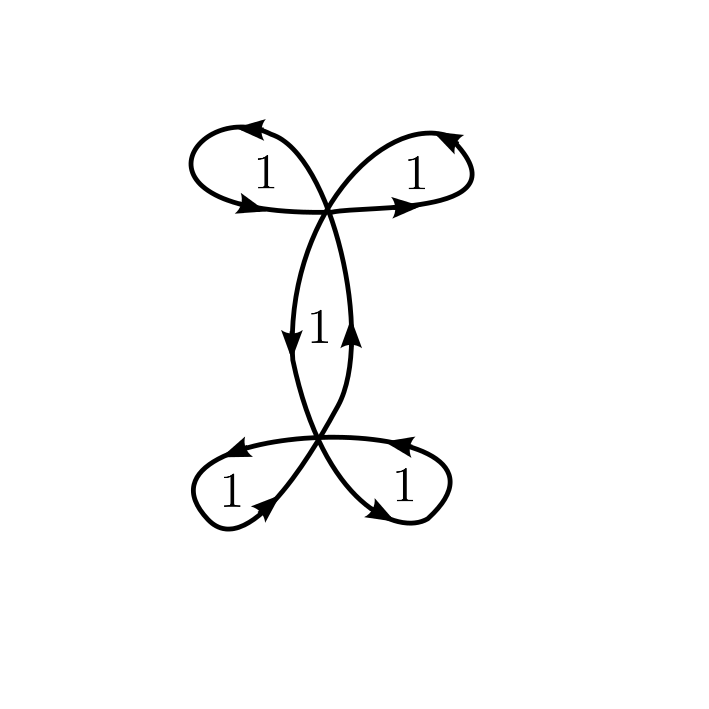
\includegraphics[width=0.25\textwidth]{40.png}
  \end{center}
\end{wrapfigure}

(2${{}^o}$) \ A componente conexa ilimitada de $\mathbb{C}\backslash\gamma^{\ast}$ contém

o complementar de um disco $D_{\rho}(  0)  $ para

algum $\rho$ suficientemente grande, donde \textsc{I}nd$_{\gamma}(  \alpha)  =0$

$\forall$ \ \ $\alpha\in%
%TCIMACRO{\U{2102} }%
%BeginExpansion
\mathbb{C}
%EndExpansion
\backslash D_{\rho}(  0)  ,$ \ o que acarreta pela
definição de $\Omega_{1}$

que $\Omega_{1}\subset D_{\rho}(0)  ,$ isto é, $\Omega_{1}$ é relativamente compacto.

Por outro lado $\Omega_{1}$ é reunião de componentes conexas

de $%
%TCIMACRO{\U{2102} }%
%BeginExpansion
\mathbb{C}
%EndExpansion
\backslash\gamma^{\ast}$ contidas em $\Omega,$ donde:

\ \ \ \ \ \ \ \ \ \ \ \ \ \ \ \ \ \ \ \ \ \ \ \ \ \ $\overline{\Omega}%
_{1}=\Omega_{1}\cup\partial\Omega_{1}\subset\Omega_{1}\cup\gamma^{\ast}%
\subset\Omega$

o que mostra que $\overline{\Omega}_{1}$ é uma parte compacta contida

em $\Omega,$ portanto (ver exerc. 4.12) \ $f$ \ tem um número

 finito de zeros em $\overline{\Omega
}_{1},$ o que prova a primei-

ra \ asserção. Se $f$ não tem zeros em $\gamma^{\ast}$ então
se verifica a hipótese de (1%
%TCIMACRO{\U{ba}}%
%BeginExpansion
${{}^o}$%
%EndExpansion
),

isto é, \ $A\cap\gamma^{\ast}=\varnothing$ e em consequência é
válida a identidade $(  8.14.2)  $ que

escrevemos assim:

\bigskip

$(  8.14.7)  $ \ \ \ \ \ \ \ \ \ $\dfrac{1}{2\pi i}\underset
{\gamma}{%
%TCIMACRO{\dint }%
%BeginExpansion
{\displaystyle\int}
%EndExpansion
}\dfrac{f^{\prime}(  z)  }{f(  z)  }dz=\underset{a\in
A\cap\Omega_{1}}{%
%TCIMACRO{\dsum }%
%BeginExpansion
{\displaystyle\sum}
%EndExpansion
\nu_{a}}$ \textsc{I}nd$_{\gamma}(  a)  +\underset{a\in
A\backslash\Omega_{1}}{%
%TCIMACRO{\dsum }%
%BeginExpansion
{\displaystyle\sum}
%EndExpansion
\nu_{a}}$ \textsc{I}nd$_{\gamma}(  a)  $ $.$

\bigskip

A hipótese $(  8.14.3)  $ e as definições de
$\Omega_{1}$ e de $Z_{f}$ implicam

$\ \ \ \ \ \ \ \ \ \underset{a\in A\cap\Omega_{1}}{%
%TCIMACRO{\dsum }%
%BeginExpansion
{\displaystyle\sum}
%EndExpansion
\nu a}$ \textsc{I}nd$_{\gamma}(  a)  =\underset{a\in A\cap
\Omega_{1}}{%
%TCIMACRO{\dsum }%
%BeginExpansion
{\displaystyle\sum}
%EndExpansion
\nu_{a}}$ $=$ $Z_{f}$ \ \ \ \ \ e \ \ \ \ \ \ $\underset{a\in A\backslash
\Omega_{1}}{%
%TCIMACRO{\dsum }%
%BeginExpansion
{\displaystyle\sum}
%EndExpansion
\nu_{a}}$ \textsc{I}nd$_{\gamma}(  a)  =0$

\bigskip

o que por $(  8.14.7)  $ prova a primeira identidade de $(
8.14.4)  .$ A segunda

identidade de $(  8.14.4)  $ é um cálculo trivial. De fato,
se indicamos com

$\left[  a,b\right]  $ o domínio de $\gamma$ então (observe que
$0\notin\Gamma^{\ast}$ pois $f$ não tem zeros

em $\gamma$)

\bigskip

\ \ \ \ \ \ \ \ \textsc{I}nd$_{\Gamma}(  0)  =\dfrac{1}{2\pi
i}\underset{\Gamma}{%
%TCIMACRO{\dint }%
%BeginExpansion
{\displaystyle\int}
%EndExpansion
}\dfrac{dz}{z}=\dfrac{1}{2\pi i}\underset{a}{%
%TCIMACRO{\dint }%
%BeginExpansion
{\displaystyle\int}
%EndExpansion
}^{b}\dfrac{\Gamma^{\prime}(  s)  }{\Gamma(  s)
}ds=\dfrac{1}{2\pi i}\underset{a}{%
%TCIMACRO{\dint }%
%BeginExpansion
{\displaystyle\int}
%EndExpansion
}^{b}\dfrac{f^{\prime}(  \gamma(  s)  )  }{f(
\gamma(  s)  )  }\gamma^{\prime}ds=$

$=\dfrac{1}{2\pi i}\underset{\gamma}{%
%TCIMACRO{\dint }%
%BeginExpansion
{\displaystyle\int}
%EndExpansion
}\dfrac{f^{\prime}(  z)  }{f(  z)  }dz$ \ $.$ $\square$

\bigskip

\textbf{Exemplo 2} \ Como ilustração do Teor. 8.14 vamos calcular a integral

\ \ \ \ \ \ \ \ \ \ \ \ \ \ \ \ \ \ \ \ \ \ \ \ \ \ \ \ \textsc{I}
$=\underset{\left\vert z\right\vert =2}{%
%TCIMACRO{\dint }%
%BeginExpansion
{\displaystyle\int}
%EndExpansion
}\dfrac{2z+1}{z^{2}+z+1}dz$

É claro que $\Omega=%
%TCIMACRO{\U{2102} }%
%BeginExpansion
\mathbb{C}
%EndExpansion
$ e o círculo $\left\vert z\right\vert =2$ satisfaz as hipóteses
$(  8.14.1)  $ e $(  8.14.3)  $

e que $\Omega_{1}=D_{2}(  0)  .$ As raízes de $f(
z)  =z^{2}+z+1=0$ são as duas raízes

cúbicas não reais $\omega_{1}$ e $\omega_{2}$ de $1$, ambas estão
contidas em $D_{2}(  0)  ,$ têm ordem

de multiplicidade igual a $1$ e o índice de cada uma delas em
relação a $\left\vert z\right\vert =2$

é $1$ \ portanto

\ \ \ \ \ \ \ \ \ \ \ \ \ \ \ \ \ \ \ \ \ \ \ \ \ \ \ \ \textsc{I} $=2\pi
i(  1\times1+1\times1)  =4\pi i$

\bigskip

\textbf{Observação \ }Sejam $\Omega,\gamma$ e $f$ como no Teor. 8.14
(1%
%TCIMACRO{\U{ba}}%
%BeginExpansion
${{}^o}$%
%EndExpansion
) e fixemos $\zeta\in\operatorname{Im}(  f)  $

arbitrário. Dizemos que $a\in\Omega$ \textit{é uma raiz de ordem }%
$\nu$ \textit{da equação }$f(  z)  =\zeta$

se $a$ é um zero de ordem $\nu$ da função $z\in\Omega\longmapsto
f(  z)  -\in%
%TCIMACRO{\U{2102} }%
%BeginExpansion
\mathbb{C}
%EndExpansion
.$ Seja agora $D$

uma parte de $\Omega$ sem ponto de acumulação tal que

(I.) \ $\ \ a$ é uma raiz de ordem $\nu_{a}$\ da equação $f(
z)  =\zeta$ \ \ $\forall$ \ $a\in D;$

(II.) \ \ $D\cap\gamma^{\ast}=\varnothing;$

(III.) \ $f(  z)  \neq\zeta$ \ para cada $z\in\Omega\backslash D.$

Então aplicando o Teor. 8.14 (1%
%TCIMACRO{\U{ba}}%
%BeginExpansion
${{}^o}$%
%EndExpansion
) à função $z\longmapsto f(  z)  -\zeta$ obtemos a fórmula

análoga a $(  8.14.2)  $

\ \ \ \ \ \ \ \ \ \ \ \ \ \ \ \ \ \ \ \ \ \ \ \ $\dfrac{1}{2\pi i}%
\underset{\gamma}{%
%TCIMACRO{\dint }%
%BeginExpansion
{\displaystyle\int}
%EndExpansion
}\dfrac{f^{\prime}(  z)  }{f(  z)  -\zeta}%
dz=\underset{a\in D}{%
%TCIMACRO{\dsum }%
%BeginExpansion
{\displaystyle\sum}
%EndExpansion
}\nu_{a}$ \textsc{I}nd$_{\gamma}(  a)  $ \ .

\bigskip

O próximo resultado é uma aplicação do Teor. 8.14 (i.e. do
teorema dos

resíduos) chamado "teorema de Rouché" que fornece o número de zeros

de uma função holomorfa $f$ num disco conhecendo o número de zeros que

tem, no mesmo disco, uma outra função holomorfa $g$ "próxima" de
$f.$ Na

realidade vamos apresentar uma versão mais geral deste teorema:

% IMAGEM 41
\begin{wrapfigure}{r}{0.25\textwidth}
  \begin{center}
    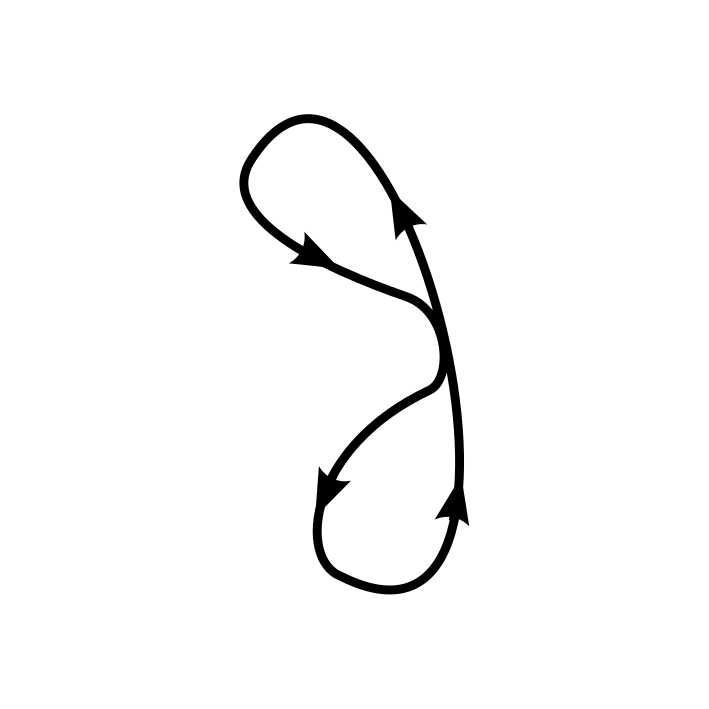
\includegraphics[width=0.25\textwidth]{41.png}
  \end{center}
\end{wrapfigure}

\bigskip

\textbf{Corolário \ 8.15} \ (Rouché) \ \textit{Sejam }$\Omega$
\textit{um aberto}

\textit{conexo e }$\gamma$ \textit{uma CSDF em} $\Omega$

\textit{verificando as condições:}

\ \ \ \ \ \ \ \ \ \ \ \ \ \ \ $\left\vert
\begin{array}
[c]{c}%
\text{\textsc{I}nd}_{\gamma}(  \alpha)  =0\text{ \ \ \ }%
\forall\text{ \ \ }\alpha\notin\Omega\text{ \ \ \ \ \ \ \ \ \ \ \ \ \ }\\
\text{\textsc{I}nd}_{\gamma}(  \alpha)  =0\text{ \ \ ou \ }1\text{
\ \ \ }\forall\text{ \ }\alpha\in\Omega\backslash\gamma^{\ast}%
\end{array}
\right.  $

\bigskip

\textit{Seja }$\Omega_{1}:=\left\{  \alpha\in\Omega\text{ }|\text{
\textsc{I}nd}_{\gamma}(  \alpha)  =1\right\}  .$ \textit{Se
}$f,g\in\mathcal{H}(  \Omega)$

\textit{ e se verifica a condição}

\bigskip

$(  8.15.1)  $ \ \ \ \ \ \ \ \ \ \ \ \ \ \ \ $\left\vert f(
z)  -g(  z)  \right\vert <\left\vert f(  z)
\right\vert $ \ \ \ $\forall$ \ $z\in\gamma^{\ast}$

\bigskip\textit{então}\ \ \ \ 

$\ \ \ \ \ \ \ \ \ \ \ \ \ \ \ \ \ \ \ \ \ \ \ \ \ \ \ \ \ \ Z_{f}=Z_{g}$ ,

\textit{onde }$Z_{f}$ (resp. $Z_{g}$) \textit{indica o número de zeros de} $f$

(resp. $g$) \textit{em }$\Omega_{1}$\textit{\ contados com sua multiplicidade.}

\bigskip

\textbf{Prova \ }A condição $(  8.15.1)  $ mostra que $g$
não é identicamente nula e que

$g$ não tem zeros em $\gamma^{\ast},$ portanto podemos aplicar o Teor.
8.14 (2%
%TCIMACRO{\U{ba}}%
%BeginExpansion
${{}^o}$%
%EndExpansion
) com

$g$ no lugar de $f,$ obtendo

\ \ \ \ \ \ \ \ \ \ \ \ \ \ \ \ \ \ $Z_{g}=\dfrac{1}{2\pi i}\underset{\gamma}{%
%TCIMACRO{\dint }%
%BeginExpansion
{\displaystyle\int}
%EndExpansion
}\dfrac{g^{\prime}(  z)  }{g(  z)  }dz=$\textsc{I}%
nd$_{\Gamma_{0}}(  0)  $

onde $\Gamma_{0}:=g\circ f.$ Seja $\Gamma:=f\circ\gamma$ e suponhamos, por
exemplo, que o domínio

de $\gamma$ é $\left[  0,1\right]  ,$ então a hipótese $(
8.15.1)  $ expressa que

\ \ \ \ \ \ \ \ \ \ \ \ \ \ \ \ \ \ \ \ \ \ \ \ $\left\vert \Gamma(
s)  -\Gamma_{0}(  s)  \right\vert <\left\vert \Gamma(
s)  \right\vert $ \ \ \ $\forall$ \ \ $s\in\left[  0,1\right]  ,$

o que pelo Lema 7.5 acarreta

\ \ \ \ \ \ \ \ \ \ \ \ \ \ \ \ \ \ \ \ \ \ \ \ \ \ \ \ \ \textsc{I}%
nd$_{\Gamma}(  0)  =$ \textsc{I}nd$_{\Gamma_{0}}(  0)  $
$.$

Finalmente, observemos que $(  8.15.1)  $ mostra que $f\neq0$ e que
$f$ não tem

zeros em $\gamma^{\ast},$ logo o Teor. 8.14 (2%
%TCIMACRO{\U{ba}}%
%BeginExpansion
${{}^o}$%
%EndExpansion
) é válido para $f,$ donde

\ \ \ \ \ \ \ \ \ \ \ \ \ \ \ \ \ \ \ \ \ \ \ \ \ \ \ \ \ \ \ \ \ \ \ \ \ $Z_{f}%
=$ \textsc{I}nd$_{\Gamma}(  0)  $ . \ $\square$

\bigskip

O próximo resultado é a "versão meromorfa" do Teor. 8.14 e é conhecido

como "Princípio do Argumento" (a razão pela qual o Teor. 8.16 é chamado

desta forma está relacionada com o conceito de'"primitiva ao longo de uma

curva" que não definiremos neste livro, ver [C], pg 120). Sejam $\Omega$
um aberto

conexo de $%
%TCIMACRO{\U{2102} }%
%BeginExpansion
\mathbb{C}
%EndExpansion
,$ $f\in\mathcal{M}(  \Omega)  ,$ $B$ o conjunto dos polos de $f$
e, para cada $b\in B,$

indiquemos com $\omega_{b}$ a ordem de $b.$ Pela Def. 8.11, $B$ não tem
ponto de acu-

mulação em $\Omega$ e então para cada compacto $K\subset\Omega,$ o
conjunto $B\cap K$ é

finito. Seja agora $X$ \ uma parte não vazia de $\Omega$ e suponhamos que
o con-

junto $B\cap X$ dos polos de $\ f$ em $X$ \textit{seja finito.} Por
definição, \textit{o número de }

\textit{polos de }$f$ \textit{em }$X$ \textit{contados com sua multiplicidade}
é o número inteiro não

negativo

\ \ \ \ \ \ \ \ \ \ \ \ \ \ \ \ \ \ \ \ \ \ $\mathcal{P}_{X}(  f)
=\mathcal{P}_{f}=\underset{b\in B\cap X}{%
%TCIMACRO{\dsum }%
%BeginExpansion
{\displaystyle\sum}
%EndExpansion
}\omega_{b}$ \ \ \ \ \ \ \ \ \ \ \ \ $(  B\cap X\text{ \ \ finito}%
)  $

\bigskip

\textbf{Teorema 8.16 \ }\textit{Sejam }$\Omega$ \textit{um aberto conexo de }$%
%TCIMACRO{\U{2102} }%
%BeginExpansion
\mathbb{C}
%EndExpansion
,$ $f\in\mathcal{M}(  \Omega)  $ \textit{tal que }$f\neq0$

\textit{e }$A$(\textit{resp. }$B$) \textit{o conjunto dos zeros }%
(\textit{resp. polos) de }$f.$\textit{\ Para cada }$a\in A$

(\textit{resp. }$b\in B$) \textit{indiquemos com }$\nu_{a}$ (\textit{resp.
}$\omega_{b}$) \textit{a ordem de }$a$ (\textit{resp. }$b$). \textit{Seja }

$\gamma$ \textit{uma CSDF em }$\Omega$ \textit{tal que}

\bigskip

$(  8.16.1)  $ \ \ \ \ \ \ \ \textsc{I}nd$_{\gamma}(
\alpha)  =0$ \ \ \ \ \ \ $\forall$ \ \ \ \ $\alpha\notin\Omega$
\ \ \ \ \ \ $(  \text{i.e. \ }\gamma\overset{\Omega}{\backsim}0)  $

\bigskip

\textit{Nestas condições valem as asseções seguintes:}

(1%
%TCIMACRO{\U{ba}}%
%BeginExpansion
${{}^o}$%
%EndExpansion
)\textit{\ \ Se }$A\cap\gamma^{\ast}=B\cap\gamma^{\ast}=\varnothing,$
\ \textit{então}

\bigskip

$(  8.16.2)  $ \ \ \ $\dfrac{1}{2\pi i}\underset{\gamma}{%
%TCIMACRO{\dint }%
%BeginExpansion
{\displaystyle\int}
%EndExpansion
}\dfrac{f^{\prime}(  z)  dz}{f(  z)  }=\underset{a\in
A}{%
%TCIMACRO{\dsum }%
%BeginExpansion
{\displaystyle\sum}
%EndExpansion
}\nu_{a}$\textsc{I}nd$_{\gamma}(  a)  -\underset{b\in B}{%
%TCIMACRO{\dsum }%
%BeginExpansion
{\displaystyle\sum}
%EndExpansion
}\omega_{b}$\textsc{I}nd$_{\gamma}(  b)  $

(2%
%TCIMACRO{\U{ba}}%
%BeginExpansion
${{}^o}$%
%EndExpansion
) \ \textit{Suponhamos que }$\gamma$ \textit{satisfaz a condição
suplementar}

\bigskip

$(  8.16.3)  $ \ \ \ \textsc{I}nd$_{\gamma}(  \alpha)
=0 $ \ \ \ \ ou \ \ \ $1$ \ \ \ \ \ \ $\forall$ \ \ \ \ $\alpha\in
\Omega\backslash\gamma^{\ast}$

\bigskip

\textit{e seja \ }$\Omega_{1}:=\left\{  \alpha\in\Omega\text{ }|\text{
\textsc{I}nd}_{\gamma}(  \alpha)  =1\right\}  .$

\textit{Então }$f$ \textit{têm um número finito de zeros e um
número finito de polos}

\textit{em }$\Omega_{1}$ (i.e. $A\cap\Omega_{1}$ e $B\cap\Omega_{1}$ são
finitos) \ \textit{e, se }$f$ \textit{não tem zeros nem }

\textit{polos em }$\gamma^{\ast},$ \textit{então}

\bigskip

$(  8.16.4)  $ \ \ \ \ \ $\dfrac{1}{2\pi i}\underset{\gamma}{%
%TCIMACRO{\dint }%
%BeginExpansion
{\displaystyle\int}
%EndExpansion
}\dfrac{f^{\prime}(  z)  }{f(  z)  }dz=Z_{f}-P_{f}$

\bigskip

\textit{onde }$Z_{f}$ (\textit{resp. }$P_{f}$) \textit{indica o número de
zeros }(\textit{resp. polos})\textit{\ de }$f$ \textit{em }$\Omega_{1}$

\textit{contados com sua multiplicidade.}

\bigskip

\textbf{Prova \ }(1%
%TCIMACRO{\U{ba}}%
%BeginExpansion
${{}^o}$%
%EndExpansion
) \ Pelo exerc.(8.11) (a), (b) e (c) temos $f^{\prime}/f\in\mathcal{M}(
\Omega)  $ \ e

\bigskip

$(  8.16.5)  $ \ \ \ \ \ \ \ \ \ \ \ \ \ \ $\left\vert
\begin{array}
[c]{c}%
\operatorname{Re}s(  f^{\prime}/f,a)  =\nu_{a}\text{ \ \ \ \ }%
\forall\text{ \ \ \ }a\in A\\
\operatorname{Re}s(  f^{\prime}/f,b)  =-\omega_{b}\text{
\ \ }\forall\text{ \ \ }b\in B
\end{array}
\right.  $

\bigskip

Pelo exerc.(8.11) (d) \ sabemos que o conjunto dos polos da função
$f^{\prime}/f$

é o conjunto $A\cup B.$ Por $(  8.16.1)  $ e por ser
$A\cap\gamma^{\ast}=B\cap\gamma^{\ast}=\varnothing,$ podemos

aplicar o Teor. 8.13 a $f^{\prime}/f$ e $\gamma$ obtendo

\bigskip\ \ \ \ \ \ \ \ \ \ \ \ \ \ \ \ \ \ \ $\dfrac{1}{2\pi i}%
\underset{\gamma}{%
%TCIMACRO{\dint }%
%BeginExpansion
{\displaystyle\int}
%EndExpansion
}\dfrac{f^{\prime}(  z)  }{f(  z)  }dz=\underset{c\in
A\cup B}{%
%TCIMACRO{\dsum }%
%BeginExpansion
{\displaystyle\sum}
%EndExpansion
}\operatorname{Re}s(  f^{\prime}/f,c)  \cdot$\textsc{I}nd$_{\gamma
}(  c)  $


o que juntos a $(  8.16.5)  $ prova $(  8.16.2)  .$

(2%
%TCIMACRO{\U{ba}}%
%BeginExpansion
${{}^o}$%
%EndExpansion
) \ Comoo $f\neq0,$ os conjuntos $A$ e $B$ não têm ponto de
acumulação em

$\Omega.$ Por outro lado, já foi demonstrado no Teor. 8.14.(2%
%TCIMACRO{\U{ba}}%
%BeginExpansion
${{}^o}$%
%EndExpansion
) que $\overline{\Omega}_{1}$ é uma

parte compacta de $\Omega,$ em consequência, os conjuntos $A\cap
\overline{\Omega}_{1}$ e $B\cap\overline{\Omega}_{1}$

são finitos, o que prova a primeira afirmação. Suponhamos agora
que $f$

não tem nem zeros nem polos em $\gamma^{\ast},$ então está
verificada a hipótese

de (1%
%TCIMACRO{\U{ba}}%
%BeginExpansion
${{}^o}$%
%EndExpansion
), logo é válida a identidade $(  8.16.2)  $ que escrevemos
da forma

seguinte:

\bigskip

$(  8.16.6)  $ \ \ \ \ \ \ $\left\vert
\begin{array}
[c]{c}%
\dfrac{1}{2\pi i}\underset{\gamma}{%
%TCIMACRO{\dint }%
%BeginExpansion
{\displaystyle\int}
%EndExpansion
}\dfrac{f^{\prime}(  z)  }{f(  z)  }dz=\underset{a\in
A\cap\Omega_{1}}{%
%TCIMACRO{\dsum }%
%BeginExpansion
{\displaystyle\sum}
%EndExpansion
\nu_{a}}\text{\textsc{I}nd}_{\gamma}(  a)  +\underset{a\in
A\backslash\Omega_{1}}{%
%TCIMACRO{\dsum }%
%BeginExpansion
{\displaystyle\sum}
%EndExpansion
\nu_{a}}\text{\textsc{I}nd}_{\gamma}(  a)  -\\
\\
-\underset{b\in B\cap\Omega_{1}}{%
%TCIMACRO{\dsum }%
%BeginExpansion
{\displaystyle\sum}
%EndExpansion
\omega_{b}}\text{\textsc{I}nd}_{\gamma}(  b)  -\underset{b\in
B\backslash\Omega_{1}}{%
%TCIMACRO{\dsum }%
%BeginExpansion
{\displaystyle\sum}
%EndExpansion
\omega_{b}}\text{\textsc{I}nd}_{\gamma}(  b)  \text{
\ \ \ \ \ \ \ \ \ \ \ \ \ \ \ \ \ \ \ \ \ }%
\end{array}
\right.  $

\bigskip

Ora, a hipótese $(  8.16.3)  $ e a s definições de
$\Omega_{1},Z_{f}$ e $P_{f}$ \ mostram que

$\ \ \ \ $

$\ \underset{a\in A\cap\Omega_{1}}{%
%TCIMACRO{\dsum }%
%BeginExpansion
{\displaystyle\sum}
%EndExpansion
\nu_{a}}$\textsc{I}nd$_{\gamma}(  a)  =\underset{a\in A\cap
\Omega_{1}}{%
%TCIMACRO{\dsum }%
%BeginExpansion
{\displaystyle\sum}
%EndExpansion
\nu_{a}}=Z_{f}$ \ \ \ \ \ \ , \ \ \ \ \ \ \ $\underset{a\in A\backslash
\Omega_{1}}{%
%TCIMACRO{\dsum }%
%BeginExpansion
{\displaystyle\sum}
%EndExpansion
\nu_{a}}$\textsc{I}nd$_{\gamma}(  a)  =0$

\bigskip

$\underset{b\in B\cap\Omega_{1}}{\text{ \ \ \ \ \ }%
%TCIMACRO{\dsum }%
%BeginExpansion
{\displaystyle\sum}
%EndExpansion
\omega_{b}}$\textsc{I}nd$_{\gamma}(  b)  =\underset{b\in
B\cap\Omega_{1}}{%
%TCIMACRO{\dsum }%
%BeginExpansion
{\displaystyle\sum}
%EndExpansion
\omega_{b}}=P_{f}$ \ \ \ \ \ ; \ \ \ \ \ \ $\underset{b\in B\backslash
\Omega_{1}}{%
%TCIMACRO{\dsum }%
%BeginExpansion
{\displaystyle\sum}
%EndExpansion
}\omega_{b}$\textsc{I}nd$_{\gamma}(  b)  =0$ \ ,

\bigskip

o que por $(  8.16.6)  $ prova $(  8.16.4)  .$
\ $\square$

\bigskip

\bigskip\ \ \ \ \ \ \ \ \ \ \ \ \ \textbf{Cálculo de integrais pelo
método dos resíduos.}

\bigskip

\bigskip

Vamos calcular integrais \textit{definidas }sem explicitar uma primitiva da função

sob o sinal de integração mas interpretando o valor da integral como uma

soma de resíduos relativos a pontos singulares de uma função meromorfa

convenientemente escolhida. Não existe um método geral de ataque do pro-

blema, assim sendo vamos nos limitar a considerar alguns tipos clássicos

de integrais mais frequentes nas aplicações. Para que um método destes

seja aplicável na prática, devemos ter um mecanismo razoavelmente efici-

ente para calcular resíduos:

\bigskip

\textbf{Proposição 8.17 \ }\textit{Sejam }$\Omega$ \textit{um aberto
de }$%
%TCIMACRO{\U{2102} }%
%BeginExpansion
\mathbb{C}
%EndExpansion
,$ $f\in\mathcal{M}(  \Omega)  ,$ $f\neq0,$ $a\in\Omega$
\textit{um}

\textit{polo de }$f$ \textit{de ordem }$m$ \textit{e}

\ \ \ \ \ \ \ \ \ \ \ \ \ \ \ \ \ \ \ \ \ \ \ \ \ \ \ \ \ \ \ \ \ $g(
z)  :=(  z-a)  ^{m}f(  z)  $ \ \ \ \ $\forall$
\ \ z$\in D_{\varepsilon}^{*}(  a)  $

(onde $D_{\varepsilon}(  a)  \subset\Omega$ é tal que
$f\in\mathcal{H}(  D_{\varepsilon}^{*}(  a)  )  $).
\textit{Então,}

\bigskip
\ \ \ \ \ \ \ \ \ \ \ \ \ \ \ \ \ \ \ \ \ \ \ \ \ \ \ \ \ \ $\operatorname{Re}%
s(  f,a)  =\dfrac{1}{(  m-1)  !}g^{(  m-1)
}(  a)  .$

\bigskip

\textit{Em particular, se }$a$ \textit{é um polo simples }(i.e. $m=1$)
\textit{de }$f$ \textit{temos: (reencon-}

\textit{tramos }o resultado do Lema 8.12 (b)):

\ \ \ \ \ \ \ \ \ \ \ \ \ \ \ \ \ \ \ \ \ \ \ \ \ \ \ \ \ $\operatorname{Re}%
s(  f,a)  =g(  a)  =\underset{z\rightarrow a}{\lim
}(  z-a)  f(  z)  $ $.$

\bigskip

\textbf{Prova \ }Como \ $a$ é uma singularidade isolada de $f,$ existe
$\varepsilon>0$ tal que

$D_{\varepsilon}(  a)  \subset\Omega$ \ e $f\in\mathcal{H}(
D_{\varepsilon}^{*}(  a)  )  ,$ portanto pela Prop. 8.5,
(2%
%TCIMACRO{\U{ba}}%
%BeginExpansion
${{}^o}$%
%EndExpansion
), (ii) existe

$g\in\mathcal{H}(  D_{\varepsilon}(  a)  )  $ tal que
$g(  a)  \neq0$ e

\bigskip

$(  8.17.1)  $ \ \ \ \ \ \ \ \ \ \ $g(  z)  =(
z-a)  ^{m}f(  z)  $ \ \ \ \ \ $\forall$ \ \ $z\in
D_{\varepsilon}^{*}(  a)  $ $.$

\bigskip

Como

\ \ \ \ \ \ \ \ \ \ \ \ \ \ \ \ \ \ \ \ \ $g(  z)  =\underset
{k\geq0}{%
%TCIMACRO{\dsum }%
%BeginExpansion
{\displaystyle\sum}
%EndExpansion
}\dfrac{1}{k!}g^{(  k)  }(  a)  (  z-a)
^{k}$ \ \ \ \ $\forall$ \ \ $z\in D_{\varepsilon}(  a)  ,$

por $(  8.17.1)  $ resulta para cada $z\in D_{\varepsilon}^{\prime
}(  a)  :$

$\ \ \ \ \ \ \ \ \ \ \ \ \ \ \ \ \ f(  z)  =\dfrac{g(
z)  }{(  z-a)  ^{m}}=\dfrac{g(  a)  }{(
z-a)  ^{m}}$ $+$ $\ldots$ $+$ $\dfrac{1}{(  m-1)  !}%
\dfrac{g^{(  m-1)  }(  a)  }{z-a}$ $\ +$

$\ \ \ +\underset{k\geq m}{%
%TCIMACRO{\dsum }%
%BeginExpansion
{\displaystyle\sum}
%EndExpansion
}\dfrac{g^{(  k)  }(  a)  }{k!}(  z-a)
^{k-m}$ \ \ \ \ \ \ o que prova que

\ \ \ \ \ \ \ \ \ \ \ \ \ \ \ \ \ \ \ \ \ \ \ \ \ $\operatorname{Re}s(
f,a)  =\dfrac{1}{(  m-1)  !}g^{(  m-1)  }(
a)  $

\bigskip

Em particular, se $m=1$ \ temos por $(  8.17.1)  $

\ \ \ \ \ \ \ \ \ \ \ \ \ \ \ \ \ \ \ \ \ \ \ 

\ \ \ \ \ \ \ \ \ \ \ \ \ \ \ \ \ \ \ \ \ \ \ \ $\operatorname{Re}s(
f,a)  =g(  a)  =\underset{z\rightarrow a}{\lim}(
z-a)  f(  z)  $ $.$ \ $\square$

\bigskip

A seguir vamos estudar vários tipos de integrais definidas calculáveis

pelo método dos resíduos

\bigskip

\textbf{Tipo 1 \ }Consideremos integrais da forma

\ \ \ \ \ \ \ \ \ \ \ \ \ \ \ \ \ \ \ \ \ \ \ \ \ \ \ \ \ \ \ \ \textrm{I}
=$\underset{0}{%
%TCIMACRO{\dint }%
%BeginExpansion
{\displaystyle\int}
%EndExpansion
}^{2\pi}R(  sent,\cos t)  dt$

onde $R:(  x,y)  \in%
%TCIMACRO{\U{211d} }%
%BeginExpansion
\mathbb{R}
%EndExpansion
^{2}\longmapsto R(  x,y)  \in%
%TCIMACRO{\U{211d} }%
%BeginExpansion
\mathbb{R}
%EndExpansion
$ denota uma função racional contínua

sobre o círculo $x^{2}+y^{2}=1.$ Seja $z=e^{it},$ então quando $t$
cresce de $0$ a $2\pi,$

$z$ percorre o círculo orientado positivamente de centro $0$ e raio 1. Como

\ \ \ \ \ \ \ \ \ \ \ \ \ \ \ \ \ \ $sent=\dfrac{1}{2i}(  z-1/z)  $
\ , \ \ $\cos t=\dfrac{1}{2}(  z+1/z)  $ \ \ e \ \ $dz=izdt$

\bigskip

a definição de integral curvilinha mostra que

\bigskip

$(  T.1.1)  $ \ \ \ \ \ \ \ \ \textrm{I} = $\underset{0}{%
%TCIMACRO{\dint }%
%BeginExpansion
{\displaystyle\int}
%EndExpansion
}^{2\pi}R(  sent,\cos t)  dt=\underset{\left\vert z\right\vert =1}{%
%TCIMACRO{\dint }%
%BeginExpansion
{\displaystyle\int}
%EndExpansion
}\dfrac{1}{iz}R\left[  \dfrac{1}{2i}(  z-1/z)  ,\dfrac{1}{2}(
z+1/z)  \right]  dz=$

$=\dfrac{1}{i}\underset{\left\vert z\right\vert =1}{%
%TCIMACRO{\dint }%
%BeginExpansion
{\displaystyle\int}
%EndExpansion
}f(  z)  dz$

onde

\bigskip

$(  T.1.2)  $ \ \ \ \ \ \ \ \ \ $f(  z)  :=\dfrac{1}%
{z}R\left[  \dfrac{1}{2i}(  z-1/z)  ,\dfrac{1}{2}(
z+1/z)  \right]  $ \ \ \ $\forall$ \ $z\in%
%TCIMACRO{\U{2102} }%
%BeginExpansion
\mathbb{C}
%EndExpansion
$ , \ onde o

segundo membro está definido.

\bigskip Ora, pelo Teor. 8.13 temos:

\bigskip

$(  T.1.3)  $ \ \ \ \ \ \ \ \ \ \ \ \ \ \ \ $\dfrac{1}{i}%
\underset{\left\vert z\right\vert =1}{%
%TCIMACRO{\dint }%
%BeginExpansion
{\displaystyle\int}
%EndExpansion
}f(  z)  dz=2\pi\underset{a\in A}{%
%TCIMACRO{\dsum }%
%BeginExpansion
{\displaystyle\sum}
%EndExpansion
}\operatorname{Re}s(  f,a)  $

sendo $A$ o conjunto dos polos de $f\in\mathcal{M}(
%TCIMACRO{\U{2102} }%
%BeginExpansion
\mathbb{C}
%EndExpansion
)  $ contidos em $D_{1}(  0)  $ (pelo

Teor. 8.13 a soma deveria ser extendida ao conjunto $D$ de todos os polos

de $f,$ porém no caso presente é claro que \textsc{I}nd$_{\left\vert
z\right\vert =1}(  a)  =0$ sempre que

$\left\vert a\right\vert >1$ portanto basta considerar o conjunto $A$ dos
polos em $D_{1}(  0)  $).

A definição de resíduo de uma função meromorfa num ponto
$a$ foi dada

apenas no caso em que o ponto é polo da função, porém como o resí-

duo de uma função $\varphi\in\mathcal{M}(  \Omega)  $ num
ponto $a\in\Omega,$ no Teor. 8.13, aparece

na forma do Lema 8.12 (a), isto é,

\ \ \ \ \ \ \ \ \ \ \ \ \ \ \ \ \ \ \ \ \ \ \ \ \ \ \ \ $\operatorname{Re}%
s(  \varphi,a)  =\dfrac{1}{2\pi i}\underset{\left\vert
z-a\right\vert =\varepsilon}{%
%TCIMACRO{\dint }%
%BeginExpansion
{\displaystyle\int}
%EndExpansion
\varphi(  z)  }dz$ \ $,$

\textit{não há inconveniente em tomar esta expressão como
definição de resí-}

\textit{duo de }$\varphi$ \textit{em }$a,$ \textit{seja ou não }$a$
\textit{um polo de }$\varphi$ (se $a$ não é polo de $\varphi$ então

$\operatorname{Re}s(  \varphi,a)  =0$). Fazendo isto, podemos
simplificar expressões do tipo

$(  T.1.3)  $ assim

\bigskip

$(  T.1.4)  $ \ \ \ \ \ \ \ \ \ \ \ \ \ \ \ \ \ \ $\dfrac{1}%
{i}\underset{\left\vert z\right\vert =1}{%
%TCIMACRO{\dint }%
%BeginExpansion
{\displaystyle\int}
%EndExpansion
}f(  z)  dz=2\pi\underset{\left\vert a\right\vert <1}{%
%TCIMACRO{\dsum }%
%BeginExpansion
{\displaystyle\sum}
%EndExpansion
}\operatorname{Re}s(  f,a)  $

\bigskip

a soma agora sendo estendida a $D_{1}(  0)  .$ Em resumo, de
$(  T.1.1)  $ e $(  T.1.4)  $

resulta

\ \ \ \ \ \ \ \ \ \ \ \ \ \ \ \ \ \ \ \ \ \ \ \textrm{I} $=\underset{0}{%
%TCIMACRO{\dint }%
%BeginExpansion
{\displaystyle\int}
%EndExpansion
}^{2\pi}R(  sent,\cos t)  dt=2\pi\underset{\left\vert a\right\vert
<1}{%
%TCIMACRO{\dsum }%
%BeginExpansion
{\displaystyle\sum}
%EndExpansion
}\operatorname{Re}s(  f,a)  $

sendo $f$ dada por $(  T.1.2)  $

\bigskip

\textbf{Exemplo \ }Calcular \textrm{I}=$\underset{0}{%
%TCIMACRO{\dint }%
%BeginExpansion
{\displaystyle\int}
%EndExpansion
}^{2\pi}\dfrac{dt}{a+sent}$ $,$ \ sendo $a\in%
%TCIMACRO{\U{211d} }%
%BeginExpansion
\mathbb{R}
%EndExpansion
$ $,$ $a>1.$

\bigskip

Neste caso $R(  x,y)  =\dfrac{1}{a+x}$ donde $f(  z)
=\dfrac{2i}{z^{2}+2aiz-1}$ \ que tem dois

polos:

\ \ \ \ \ \ \ \ \ $z_{1}=i(  -a+\sqrt{a^{2}-1})  $ \ \ \ \ e
\ \ \ $z_{2}=i(  -a-\sqrt{a^{2}-1})  $ $.$

\bigskip

Como $\left\vert z_{2}\right\vert >1$ \ e \ $\left\vert z_{1}\right\vert <1$ temos

\ \ \ \ \ \ \ \ \ \ \ \ \ \ \ \ \ \ \ \ \ \ \ \ \ \ \ \ \textrm{I}=$\dfrac
{1}{i}\underset{\left\vert z\right\vert =1}{%
%TCIMACRO{\dint }%
%BeginExpansion
{\displaystyle\int}
%EndExpansion
}f(  z)  dz=2\pi\operatorname{Re}s(  f,z_{1})
=\dfrac{2\pi}{\sqrt{a^{2}-1}}$

\bigskip

\textbf{Tipo 2} \ Integrais do tipo

\ \ \ \ \ \ \ \ \ \ \ \ \ \ \ \ \ \ \ \ \ \ \ \ \ \ \ \ \ \ \ \ \ \ \ \ \ \ \textrm{I}
$=\underset{-\infty}{%
%TCIMACRO{\dint \nolimits^{+\infty}}%
%BeginExpansion
{\displaystyle\int\nolimits^{+\infty}}
%EndExpansion
}R(  x)  dx$

onde $R(  x)  =\dfrac{a_{n}x^{n}+\text{ }\ldots\text{ }+a_{0}%
}{b_{m}x^{m}+\text{ }\ldots+b_{0}}$ \ é uma função racional sem
polos no eixo

real. Devemos supor que \textrm{I} \ é convergente, isto é, a parte
principal de

$R(  x)  $ no infinito que é

\ \ \ \ \ \ \ \ \ \ \ \ \ \ \ \ \ \ \ \ \ \ \ \ \ \ \ \ \ \ \ \ \ \ \ \ \ \ $\dfrac
{x^{n}}{x^{m}}=\dfrac{1}{x^{m-n}}$

deve ser do tipo $1/x^{p}$ \ com $p\geq2$ \ logo \ $m\geq n+2$ .\\

% IMAGEM 42
\begin{center}
  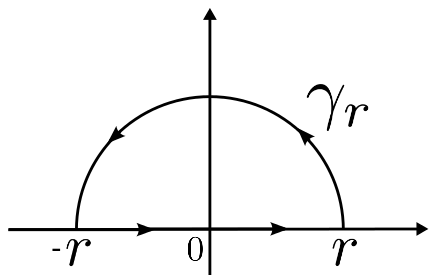
\includegraphics[width=0.3\textwidth]{42.png}
\end{center}

Sejam $\gamma_{r}:t\in\left[  0,\pi\right]  \longmapsto re^{it}\in%
%TCIMACRO{\U{2102} }%
%BeginExpansion
\mathbb{C}
%EndExpansion
$ \ e \ $\Gamma_{r}:=\left[  -r,r\right]  \vee\gamma_{r}$ \ \ $\forall$
\ $r>0$ \ então

pelo Teor. 8.13 podemos escrever

\bigskip

$(  T.2.1)  $ \ \ $\underset{\gamma_{r}}{%
%TCIMACRO{\dint }%
%BeginExpansion
{\displaystyle\int}
%EndExpansion
}R(  z)  dz=\underset{-r}{%
%TCIMACRO{\dint \nolimits^{r}}%
%BeginExpansion
{\displaystyle\int\nolimits^{r}}
%EndExpansion
}R(  x)  dx+\underset{\gamma_{r}}{%
%TCIMACRO{\dint }%
%BeginExpansion
{\displaystyle\int}
%EndExpansion
}R(  z)  dz=2\pi i\underset{\operatorname{Im}(  a)  >0}{%
%TCIMACRO{\dsum }%
%BeginExpansion
{\displaystyle\sum}
%EndExpansion
}$ $\operatorname{Re}s(  R,a)  $\ \ \ $\forall$ \ 

\ 

$r>r_{0}$ onde todas as raízes de $b_{m}z^{m}+$ $\ldots+b_{0}=0$ (\ i.e.
polos de $R$) estão

contidos no disco $D_{r_{0}}(  0)  $

Vamos provar que

\bigskip\ $(  T.2.2)  $
\ \ \ \ \ \ \ \ \ \ \ \ \ \ \ \ \ \ \ \ \ \ \ \ \ $\underset{r\rightarrow
+\infty}{\lim}\underset{\gamma_{r}}{%
%TCIMACRO{\dint }%
%BeginExpansion
{\displaystyle\int}
%EndExpansion
}R(  z)  dz=0$

\bigskip De fato,

\ \ \ \ \ \ \ \ \ \ \ \ \ \ \ \ $\left\vert R(  z)  \right\vert
=\left\vert \dfrac{z^{n}}{z^{m}}\cdot\dfrac{a_{n}+a_{m-1}z^{-1}+\text{ }%
\ldots+a_{0}z^{-n}}{b_{m}+b_{m-1}z^{-1}+\text{ }\ldots+b_{0}z^{-m}}\right\vert
$

\bigskip

portanto se $M>\left\vert \dfrac{a_{n}}{b_{m}}\right\vert ,$\ existe $N>0$ tal
que $\forall$ \ $r>N$ \ temos

\bigskip

\ \ \ \ \ \ \ \ \ \ \ \ \ \ \ \ \ \ \ \ \ \ \ \ \ $\left\vert R(
z)  \right\vert \leq Mr^{n-m}$ \ \ sempre que $\left\vert z\right\vert
=r$

donde

\ \ \ \ \ \ \ \ \ \ \ \ \ \ \ \ \ \ \ \ \ \ \ \ \ $\left\vert \underset
{\gamma_{r}}{%
%TCIMACRO{\dint }%
%BeginExpansion
{\displaystyle\int}
%EndExpansion
}R(  z)  dz\right\vert \leq\underset{0}{%
%TCIMACRO{\dint \nolimits^{\pi}}%
%BeginExpansion
{\displaystyle\int\nolimits^{\pi}}
%EndExpansion
}Mr^{n-m}rdt=\dfrac{M\pi}{r^{m-n-1}}$

\bigskip

e como $m\geq n+2$ e portanto \ $m-n-1>0,$ resulta $(  T.2.2)  .$

Como

\ \ \ \ \ \ \ \ \ \ \ \ \ \ \ \ \ \ \ \ \ \ \ \textrm{I} $=\underset
{r\rightarrow+\infty}{\lim}\underset{-r}{%
%TCIMACRO{\dint \nolimits^{r}}%
%BeginExpansion
{\displaystyle\int\nolimits^{r}}
%EndExpansion
}R(  x)  dx,$

de $(  T.2.1)  $ e $(  T.2.2)  $ \ segue

\bigskip

$(  T.2.3)  $ \ \ \ \ \ \ \ \ \ \ \ \ \ \ \ \ \ \ \ \ \textrm{I}
$=\underset{-\infty}{%
%TCIMACRO{\dint \nolimits^{+\infty}}%
%BeginExpansion
{\displaystyle\int\nolimits^{+\infty}}
%EndExpansion
}R(  x)  dx=2\pi i\underset{\operatorname{Im}(  a)  >0}{%
%TCIMACRO{\dsum }%
%BeginExpansion
{\displaystyle\sum}
%EndExpansion
}\operatorname{Re}s(  R,a)  $

\bigskip

Observar que poderíamos ter trabalhado no semiplano $\operatorname{Im}%
(  a)  <0,$ bastan-

do para isto considerar $\widetilde{\gamma}_{r}:t\in\left[  0,\pi\right]
\longmapsto re^{-it}\in%
%TCIMACRO{\U{2102} }%
%BeginExpansion
\mathbb{C}
%EndExpansion
$ \ e \ $\widetilde{\Gamma}_{r}=\left[  -r,r\right]  \vee\widetilde{\gamma
}_{r}.$

Neste caso, para os pontos $a$ \ "interiores a $\widetilde{\Gamma}_{r}"$ temos
\textsc{I}nd$_{\widetilde{\Gamma}_{r}}(  a)  =-1$ \ e

então, em vez de $(  T.2.3)  $ teríamos

\ \ \ \ \ \ \ \ \ \ \ \ \ \ \textrm{I} $=\underset{-\infty}{%
%TCIMACRO{\dint \nolimits^{+\infty}}%
%BeginExpansion
{\displaystyle\int\nolimits^{+\infty}}
%EndExpansion
}R(  x)  dx=-2\pi i\underset{\operatorname{Im}(  a)
<0}{%
%TCIMACRO{\dsum }%
%BeginExpansion
{\displaystyle\sum}
%EndExpansion
}\operatorname{Re}s(  R,a)  $ \ $.$

\bigskip

\textbf{Exemplo: \ }Calcular \textrm{I} $=\underset{0}{%
%TCIMACRO{\dint ^{+\infty}}%
%BeginExpansion
{\displaystyle\int^{+\infty}}
%EndExpansion
}\dfrac{dx}{1+x^{6}}$

% imagem 43
\begin{wrapfigure}{r}{0.35\textwidth}
  \begin{center}
    \includegraphics[width=0.35\textwidth]{43.png}
  \end{center}
\end{wrapfigure}

Como \ \textrm{I} $=\dfrac{1}{2}\underset{-\infty}{%
%TCIMACRO{\dint \nolimits^{+\infty}}%
%BeginExpansion
{\displaystyle\int\nolimits^{+\infty}}
%EndExpansion
}\dfrac{dx}{1+x^{6}},$ a integral do exem-

plo pode ser considerada do Tipo 2. Vamos 

determinar os polos de $R(  z)  =\dfrac{1}{1+z^{6}}$\ 

que são pontos de anulação de $z^{6}+1.$ \ De 

$z^{6}=-1=e^{i\pi}$ \ resulta $z_{k}=e^{\tfrac{i}{6}(  \pi+2k\pi)  }$ \ $,$

\ $k=$\ $0,1,2,3,4,$ e $5$ \ \ logo só $z_{0}=e^{\tfrac{i\pi}{6}}$ $,$ 

$z_{1}=e^{\tfrac{i\pi}{2}}$ e $z_{2}=e^{\tfrac{5i\pi}{6}}$ pertencem ao 

semiplano $\operatorname{Im}(  z)  >0.$ Resulta então

\bigskip

\textrm{I} $=\dfrac{1}{2}\underset{-\infty}{%
%TCIMACRO{\dint \nolimits^{+\infty}}%
%BeginExpansion
{\displaystyle\int\nolimits^{+\infty}}
%EndExpansion
}\dfrac{dx}{1+x^{6}}=\pi i\underset{k=0}{\overset{2}{%
%TCIMACRO{\dsum }%
%BeginExpansion
{\displaystyle\sum}
%EndExpansion
}}\operatorname{Re}s(  \dfrac{1}{1+z^{6}},z_{k})  $

\bigskip

$\operatorname{Re}s(  \dfrac{1}{1+z^{6}},z_{k})
=\underset{z\rightarrow z_{k}}{\lim}(  z-z_{k})  \dfrac{1}{1+z^{6}%
}=\underset{z\rightarrow z_{k}}{\lim}\dfrac{1}{\dfrac{1+z^{6}}{z-z_{k}}}=$

$\underset{z\rightarrow z_{k}}{\lim}\dfrac{1}{z^{5}+z_{k}z^{4}+z_{k}^{2}%
z^{3}+z_{k}^{3}z^{2}+z_{k}^{4}z+z_{k}^{5}}=\dfrac{1}{6z_{k}^{5}}=-\dfrac
{z_{k}}{6}$ \ pois \ $z_{k}^{6}=-1$ \ \ \ logo

\bigskip

\ \ \ \ \ \ \ \ \ \ \ \ \ \ $\operatorname{Re}s(  \dfrac{1}{1+z^{6}%
},z_{0})  =-\dfrac{z_{o}}{6}=-\dfrac{1}{6}e^{\tfrac{i\pi}{6}}$

\ \ \ \ \ \ \ \ \ \ \ \ \ \ $\operatorname{Re}s(  \dfrac{1}{1+z^{6}%
},z_{1})  =-\dfrac{z_{1}}{6}=-\dfrac{1}{6}e^{\tfrac{i\pi}{2}}$

\ \ \ \ \ \ \ \ \ \ \ \ \ \ $\operatorname{Re}s(  \dfrac{1}{1+z^{6}%
},z_{2})  =-\dfrac{z_{2}}{6}=-\dfrac{1}{6}e^{\tfrac{5i\pi}{6}}$

\bigskip

portanto \ \ \ \ \ \ \ \ \ \ \ \ \ \ \textrm{I} $=-\dfrac{\pi i}{6}(
e^{\tfrac{i\pi}{6}}+e^{\tfrac{i\pi}{2}}+e^{\tfrac{5\pi i}{6}})
=\dfrac{\pi}{3}$ \ $.$

\bigskip

\textbf{Tipo 3 \ }Integrais do tipo

\ \ \ \ \ \ \ \ \ \ \ \ \ \ \ \ \ \ \ \ \ \ \ \ \ \ \ \ \textrm{I }%
$=\underset{-\infty}{%
%TCIMACRO{\dint \nolimits^{+\infty}}%
%BeginExpansion
{\displaystyle\int\nolimits^{+\infty}}
%EndExpansion
}e^{ix}\cdot f(  x)  dx $

onde $f\in\mathcal{M}(  \Omega)  ,$ $\Omega$ é um aberto que
contem o semiplano

\ \ \ \ \ \ \ \ \ \ \ \ \ \ \ \ \ \ \ \ \ \ \ $\left\{  z\in%
%TCIMACRO{\U{2102} }%
%BeginExpansion
\mathbb{C}
%EndExpansion
\text{ }|\text{ }\operatorname{Im}(  z)  \geq0\right\}  ,$

$f$ tem apenas \textit{número finito }\ de polos no semiplano aberto

\ \ \ \ \ \ \ \ \ \ \ \ \ \ \ \ \ \ \ \ \ \ \ \ $%
%TCIMACRO{\dprod }%
%BeginExpansion
{\displaystyle\prod}
%EndExpansion
:=\left\{  z\in%
%TCIMACRO{\U{2102} }%
%BeginExpansion
\mathbb{C}
%EndExpansion
\text{ }|\text{ }\operatorname{Im}(  z)  >0\right\}  $

e

$\bigskip$

$(  T.3.1)  $ \ \ \ \ \ \ \ \ \ \ \ \ \ \ $\underset{\left\vert
z\right\vert \rightarrow+\infty}{\lim}f(  z)  =0$ $.$

É claro então que existe $\rho>0$ tal que todos os polos de $f$ (em $%
%TCIMACRO{\dprod }%
%BeginExpansion
{\displaystyle\prod}
%EndExpansion
)$ estão

em $D_{\rho}(  0)  .$ Seja agora $r>\rho$ arbitrário e consideremos

\ \ \ \ \ \ \ \ \ \ \ \ \ \ 

\ \ \ \ \ \ \ \ \ \ \ \ \ $\gamma_{r}:t\in\left[  0,\pi\right]  \longmapsto
re^{it}\in%
%TCIMACRO{\U{2102} }%
%BeginExpansion
\mathbb{C}
%EndExpansion
$ \ \ e \ \ $\Gamma_{r}:=\left[  -r,r\right]  \vee\gamma_{r}$ $,$

\bigskip

então, pelo Teor. 8.13 resulta

$\bigskip$

$\underset{\gamma_{r}}{%
%TCIMACRO{\dint }%
%BeginExpansion
{\displaystyle\int}
%EndExpansion
}e^{iz}f(  z)  dz=\underset{\left[  -r,r\right]  }{%
%TCIMACRO{\dint }%
%BeginExpansion
{\displaystyle\int}
%EndExpansion
}e^{ix}f(  x)  dx+\underset{\gamma_{r}}{%
%TCIMACRO{\dint }%
%BeginExpansion
{\displaystyle\int}
%EndExpansion
}e^{iz}f(  z)  dz=2\pi i\underset{\operatorname{Im}(
a)  >0,\left\vert a\right\vert <\rho}{%
%TCIMACRO{\dsum }%
%BeginExpansion
{\displaystyle\sum}
%EndExpansion
}\operatorname{Re}s(  e^{iz}f(  z)  ,a)  $.

\bigskip

Portanto, tomando limites para $r\rightarrow+\infty$ obtemos

\bigskip

$(  T.3.2)  $ \ \ $\underset{-\infty}{%
%TCIMACRO{\dint \nolimits^{+\infty}}%
%BeginExpansion
{\displaystyle\int\nolimits^{+\infty}}
%EndExpansion
}e^{ix}f(  x)  dx+\underset{r\rightarrow+\infty}{\lim}%
\underset{\gamma_{r}}{%
%TCIMACRO{\dint }%
%BeginExpansion
{\displaystyle\int}
%EndExpansion
}e^{iz}f(  z)  dz=2\pi i\underset{\operatorname{Im}(
a)  >0}{%
%TCIMACRO{\dsum }%
%BeginExpansion
{\displaystyle\sum}
%EndExpansion
}\operatorname{Re}s(  e^{iz}f(  z)  ,a)  $

\bigskip

Mostremos que a segunda parcela do 1%
%TCIMACRO{\U{ba} }%
%BeginExpansion
${{}^o}$
%EndExpansion
membro de $(  T.3.2)  $ é nula. Seja

$M(  r)  :=\sup\left\{  \left\vert f(  z)  \right\vert
\text{ }|\text{ }z\in\Omega\text{ e }\left\vert z\right\vert =r\right\}  ,$
então de $(  T.3.1)  $ segue

\bigskip

$(  T.3.3)  $
\ \ \ \ \ \ \ \ \ \ \ \ \ \ \ \ \ \ \ \ \ \ \ \ \ \ \ $\underset
{r\rightarrow\infty}{\lim}M(  r)  =0$

\bigskip

e então

$\ \ \ \ \ \ \ \ \ \ \ \ \ \ \ \ \ \ \ \ \ \ \ \ \ \ \ \ \ \left\vert
\underset{\gamma_{r}}{%
%TCIMACRO{\dint }%
%BeginExpansion
{\displaystyle\int}
%EndExpansion
}e^{iz}f(  z)  dz\right\vert =\left\vert \underset{0}{%
%TCIMACRO{\dint \nolimits^{\pi}}%
%BeginExpansion
{\displaystyle\int\nolimits^{\pi}}
%EndExpansion
}e^{ir(  \cos t+isent)  }\cdot f(  re^{it})
rie^{it}dt\right\vert =$



$=\left\vert \underset{0}{%
%TCIMACRO{\dint \nolimits^{\pi}}%
%BeginExpansion
{\displaystyle\int\nolimits^{\pi}}
%EndExpansion
}e^{ir\cos t}\cdot e^{-rsent}f(  rie^{it})  dt\right\vert \leq
M(  r)  r\underset{0}{%
%TCIMACRO{\dint \nolimits^{\pi}}%
%BeginExpansion
{\displaystyle\int\nolimits^{\pi}}
%EndExpansion
}e^{-rsent}dt=2M(  r)  r\underset{0}{%
%TCIMACRO{\dint \nolimits^{\pi/2}}%
%BeginExpansion
{\displaystyle\int\nolimits^{\pi/2}}
%EndExpansion
}e^{-rsent}dt$\\

% imagem 44
\begin{wrapfigure}[1]{r}{0.5\textwidth}
  \begin{center}
    \includegraphics[width=0.5\textwidth]{44.png}
  \end{center}
\end{wrapfigure}

\bigskip

É claro (ver figura) que

$\bigskip$

$-sent\leq-\dfrac{2}{\pi}t$ \ \ \ \ \ $\forall$ \ \ $t\in\left[
0,\pi/2\right]  $

\bigskip

e então

$\ \ \ \ \ \ \ \ $

$\ $

$\ \underset{0}{%
%TCIMACRO{\dint \nolimits^{\pi/2}}%
%BeginExpansion
{\displaystyle\int\nolimits^{\pi/2}}
%EndExpansion
}e^{-rsent}dt\leq\underset{0}{%
%TCIMACRO{\dint }%
%BeginExpansion
{\displaystyle\int}
%EndExpansion
}^{\pi/2}e^{-\tfrac{2rt}{\pi}}dt=$

$\dfrac{\pi}{2r}(  1-e^{-r})
\leq\dfrac{\pi}{2r}$ \ $,$\\

\bigskip

em consequência $\left\vert \underset{\gamma_{r}}{{\displaystyle\int}}e^{iz}f(  z)  dz\right\vert \leq2M( r)  r\cdot\dfrac{\pi}{2r}=M(r) \pi$


o que, por $(T.3.3)$, implica que

$$\underset{r\rightarrow+\infty}{\lim}\underset{\gamma_{r}}{{\displaystyle\int}}e^{iz}f(z)dz=0$$

e então, por $(T.3.2)$, vem:

\bigskip

$(T.3.4)$ $\underset{-\infty}{{\displaystyle\int\nolimits^{+\infty}}}e^{ix}f(x)dx=2\pi i\underset{\operatorname{Im}(a)>0}{{\displaystyle\sum}}\operatorname{Re}s(e^{iz}f(z),a)$

\bigskip

A seguir vamos calcular integrais do tipo 3 admitindo que $f$ tem também

um polo simples na origem:

\bigskip

\textbf{Tipo 4} \ Integrais do tipo\\

\ \ \ \ \ \ \ \ \ \ \ \ \ \ \ \ \ \ \ \ \ \ \ \ \ \ \ \ \ \ \ \ \ \ \ \ \ \ \ \ \ \ \textrm{I}
$=\underset{-\infty}{%
%TCIMACRO{\dint \nolimits^{+\infty}}%
%BeginExpansion
{\displaystyle\int\nolimits^{+\infty}}
%EndExpansion
}e^{ix}f(  x)  dx$\\

onde $f\in\mathcal{M}(  \Omega)  $, $\Omega$ sendo um aberto que
contém o semiplano $\{z\in%
%TCIMACRO{\U{2102} }%
%BeginExpansion
\mathbb{C}
%EndExpansion
$ $|$

$\operatorname{Im}(  z)  \geq0\},$ $f$ tem um polo simples na
origem e um número finito de polos

no semiplano aberto $\left\{  z\in%
%TCIMACRO{\U{2102} }%
%BeginExpansion
\mathbb{C}
%EndExpansion
\text{ }|\text{ }\operatorname{Im}(  z)  >0\right\}  $ \ e

\bigskip

$(  T.4.1)  $
\ \ \ \ \ \ \ \ \ \ \ \ \ \ \ \ \ \ \ \ \ \ \ \ \ \ $\underset{\left\vert
z\right\vert \rightarrow+\infty}{\lim}f(  z)  =0$ $.$

\bigskip

% imagem 45
\begin{wrapfigure}{r}{0.3\textwidth}
  \begin{center}
    \includegraphics[width=0.3\textwidth]{45.png}
  \end{center}
\end{wrapfigure}

Vamos precisar do seguinte:

\bigskip



\textbf{Lema 8.18 \ }\textit{Sejam }$a\in\mathbb{C},\rho>0,f\in\mathcal{H}(D_{\rho}^{*}(a))$


\textit{e suponhamos que }$a$ \textit{é um polo simples de} $f$.


\textit{Se }$0<\varepsilon<\rho$ \textit{e} $\gamma_{\varepsilon}:t\in\left[  0,\pi\right]  \longmapsto a+\varepsilon e^{it}\in\mathbb{C}$,

\textit{então}

\ \ \ \ \ \ \ $\underset
{\varepsilon\rightarrow0}{\lim}\underset{\gamma_{\varepsilon}}{\text{ }%
%TCIMACRO{\dint }%
%BeginExpansion
{\displaystyle\int}
%EndExpansion
}f(  z)  dz=\pi i\operatorname{Re}s(  f,a)  $ $.$\\\\

\bigskip

\textbf{Prova \ }Existe $h\in\mathcal{H}(  D_{\rho}(  a))  $ al que


$\ \ \ \ \ \ \  f(z)  =\dfrac{\operatorname{Re}s(  f,a)  }{z-a}+h(z)  $ \ \ \ \ $\forall$ \ \ $z\in D_{\rho}^{*}(  a)  $

donde\\

$\underset{\gamma_{\varepsilon}}{{\displaystyle\int}}f(  z)  dz=\operatorname{Re}s(  f,a)  \underset{0}{{\displaystyle\int\nolimits^{\pi}}n}idt+\underset{0}{{\displaystyle\int\nolimits^{\pi}}}h(  a+\varepsilon e^{it})  \varepsilon ie^{it}dt$

$=\pi\operatorname{Re}s(  f,a)  +\varepsilon i\underset{0}{{\displaystyle\int\nolimits^{\pi}}}h(  a+\varepsilon e^{it})  e^{it}dt$ , o que prova o resultado

pois $h$ é localmente limitada em $a$ $.$ \ $\square$

\bigskip

Voltemos ao cálculo de \textrm{I. }Naturalmente vamos supor, por
hipótese, que \textrm{I}

existe, isto é, existe e é finito o limite duplo

$\ \ \ \underset{\underset{r\rightarrow+\infty}{\varepsilon\rightarrow\infty}%
}{\lim}\left\{  \underset{-r}{%
%TCIMACRO{\dint \nolimits^{-\varepsilon}}%
%BeginExpansion
{\displaystyle\int\nolimits^{-\varepsilon}}
%EndExpansion
}e^{ix}f(  x)  dx+\underset{\varepsilon}{%
%TCIMACRO{\dint \nolimits^{r}}%
%BeginExpansion
{\displaystyle\int\nolimits^{r}}
%EndExpansion
}e^{ix}f(  x)  dx\right\}  =\underset{-\infty}{%
%TCIMACRO{\dint \nolimits^{0}}%
%BeginExpansion
{\displaystyle\int\nolimits^{0}}
%EndExpansion
}e^{ix}f(  x)  dx+\underset{0}{%
%TCIMACRO{\dint \nolimits^{+\infty}}%
%BeginExpansion
{\displaystyle\int\nolimits^{+\infty}}
%EndExpansion
}e^{ix}f(  x)  dx=$

$\bigskip$

$=\underset{-\infty}{%
%TCIMACRO{\dint \nolimits^{+\infty}}%
%BeginExpansion
{\displaystyle\int\nolimits^{+\infty}}
%EndExpansion
}e^{ix}f(  x)  dx=\mathrm{I}$

Dado $\delta>0$ arbitário, seja $\gamma_{\delta}:t\in\left[  0,\pi\right]
\longmapsto\delta e^{it}\in%
%TCIMACRO{\U{2102} }%
%BeginExpansion
\mathbb{C}
%EndExpansion
,$

então consideremos a seguinte CSDF

% IMAGEM 46

  \begin{center}
    \includegraphics[width=0.25\textwidth]{46.png}
  \end{center}


Se $g(  z)  :=e^{iz}f(  z)  ,$ \ pelo Teor. 8.13 temos

$\ \ \ \ \ \ \ \ \ \ \ \ \ \ \ \underset{\gamma}{%
%TCIMACRO{\dint }%
%BeginExpansion
{\displaystyle\int}
%EndExpansion
}g(  z)  dz=\underset{\left[  -r,-\varepsilon\right]  }{%
%TCIMACRO{\dint }%
%BeginExpansion
{\displaystyle\int}
%EndExpansion
}+\underset{\gamma_{\varepsilon}^{\circ}}{%
%TCIMACRO{\dint }%
%BeginExpansion
{\displaystyle\int}
%EndExpansion
}+\underset{\left[  \varepsilon,r\right]  }{%
%TCIMACRO{\dint }%
%BeginExpansion
{\displaystyle\int}
%EndExpansion
}+\underset{\gamma_{r}}{%
%TCIMACRO{\dint }%
%BeginExpansion
{\displaystyle\int}
%EndExpansion
}=2\pi i\underset{\operatorname{Im}(  a)  >0}{%
%TCIMACRO{\dsum }%
%BeginExpansion
{\displaystyle\sum}
%EndExpansion
}\operatorname{Re}s(  g,a)  $

o que podemos escrever assim

\bigskip

$\underset{-r}{%
%TCIMACRO{\dint \nolimits^{-\varepsilon}}%
%BeginExpansion
{\displaystyle\int\nolimits^{-\varepsilon}}
%EndExpansion
}e^{ix}f(  x)  dx+\underset{\varepsilon}{%
%TCIMACRO{\dint \nolimits^{r}}%
%BeginExpansion
{\displaystyle\int\nolimits^{r}}
%EndExpansion
}e^{ix}f(  x)  dx+\underset{_{\gamma_{r}}}{%
%TCIMACRO{\dint }%
%BeginExpansion
{\displaystyle\int}
%EndExpansion
}g(  z)  dz=\underset{\gamma_{\varepsilon}}{%
%TCIMACRO{\dint }%
%BeginExpansion
{\displaystyle\int}
%EndExpansion
}g(  z)  dz+2\pi i\underset{\operatorname{Im}(  a)  >0}{%
%TCIMACRO{\dsum }%
%BeginExpansion
{\displaystyle\sum}
%EndExpansion
}\operatorname{Re}s(  g,a)  $

\bigskip

Tomando limites para r$\rightarrow+\infty$ \ e \ $\varepsilon\rightarrow0^{+}%
$, e levando em consideração que

da mesma forma que no caso anterior (já que $(  T.3.1)
=(  T.4.1)  $):

\ \ \ \ \ \ \ \ \ \ \ \ \ \ \ \ \ \ \ \ \ \ \ \ \ \ \ \ \ \ $\underset
{r\rightarrow+\infty}{\lim}\underset{\gamma_{r}}{%
%TCIMACRO{\dint }%
%BeginExpansion
{\displaystyle\int}
%EndExpansion
}g(  z)  dz=0$ $,$

por $(  T.4.1)  $ e pelo Lema 8.18, obtemos:

\bigskip

$(  T.4.2)  $ \ \ \ \ \ \ \ \ \ $\underset{-\infty}{%
%TCIMACRO{\dint \nolimits^{+\infty}}%
%BeginExpansion
{\displaystyle\int\nolimits^{+\infty}}
%EndExpansion
}e^{ix}f(  x)  dx=\pi i\operatorname{Re}s(  g,0)  +2\pi
i\underset{\operatorname{Im}(  a)  >0}{%
%TCIMACRO{\dsum }%
%BeginExpansion
{\displaystyle\sum}
%EndExpansion
}\operatorname{Re}s(  g,a)  $ $.$

\bigskip

\textbf{Exemplo: \ }Calcular

\ \ \ \ \ \ \ \ \ \ \ \ \ \ \ \ \ \ \ \ \ \ \ \ \ \ \ \ \ \ \ \ \ \ \ \ \ \textrm{I
}$=\underset{-\infty}{%
%TCIMACRO{\dint \nolimits^{+\infty}}%
%BeginExpansion
{\displaystyle\int\nolimits^{+\infty}}
%EndExpansion
}\dfrac{e^{ix}}{x}dx$

Como único polo de $g(  z)  =\dfrac{e^{iz}}{z}$ \ é na
origem, a 2%
%TCIMACRO{\U{aa} }%
%BeginExpansion
${{}^a}$
%EndExpansion
parcela do 2%
%TCIMACRO{\U{ba} }%
%BeginExpansion
${{}^o}$
%EndExpansion
membro

de $(  T.4.2)  $ é nula, donde

\ \ \ \ \ \ \ \ \ \ \ \ \ \ \ \ \ \ \ \ \ \ \ \ \ \ \ \ \ \ \ \ \ \ \ $\underset
{-\infty}{%
%TCIMACRO{\dint \nolimits^{+\infty}}%
%BeginExpansion
{\displaystyle\int\nolimits^{+\infty}}
%EndExpansion
}\dfrac{e^{ix}}{x}dx=\pi i\operatorname{Re}s(  \dfrac{e^{iz}}%
{z},0)  $

e sendo

\ \ \ \ \ \ \ \ \ \ \ \ \ \ \ \ \ \ \ \ \ \ \ \ \ $\dfrac{e^{iz}}{z}=\dfrac
{1}{z}+i-\dfrac{z^{2}}{2!}+$ $\ldots\ldots$ \ \ $\implies$
\ $\operatorname{Re}s(  \dfrac{e^{iz}}{z},0)  =1$

o que implica

\ \ \ \ \ \ \ \ \ \ \ \ \ \ \ \ \ \ \ \ \ \ \ \ $\underset{-\infty}{%
%TCIMACRO{\dint \nolimits^{+\infty}}%
%BeginExpansion
{\displaystyle\int\nolimits^{+\infty}}
%EndExpansion
}\dfrac{e^{ix}}{x}dx=\pi i$ $.$

A relação acima junto com

\ \ \ \ \ \ \ \ \ \ \ \ \ \ \ \ \ \ \ \ \ \ \ \ \ \ \ \ \ \ \ \ \ \ \ \ \ \ \ $\dfrac
{e^{ix}}{x}=\dfrac{\cos x+isenx}{x}$\ \ 

acarreta

\ \ \ \ \ \ \ \ \ \ \ \ \ \ \ \ \ $\underset{-\infty}{%
%TCIMACRO{\dint \nolimits^{+\infty}}%
%BeginExpansion
{\displaystyle\int\nolimits^{+\infty}}
%EndExpansion
}\dfrac{\cos x}{x}dx=0$ \ \ \ \ \ \ \ \ \ , \ \ \ \ \ \ \ \ \ \ \ $\underset
{-\infty}{%
%TCIMACRO{\dint \nolimits^{+\infty}}%
%BeginExpansion
{\displaystyle\int\nolimits^{+\infty}}
%EndExpansion
}\dfrac{senx}{x}dx=\pi$

e

\ \ \ \ \ \ \ \ \ \ \ \ \ \ \ \ \ $\underset{0}{%
%TCIMACRO{\dint \nolimits^{+\infty}}%
%BeginExpansion
{\displaystyle\int\nolimits^{+\infty}}
%EndExpansion
}\dfrac{senx}{x}dx=\dfrac{1}{2}\underset{-\infty}{%
%TCIMACRO{\dint \nolimits^{+\infty}}%
%BeginExpansion
{\displaystyle\int\nolimits^{+\infty}}
%EndExpansion
}\dfrac{senx}{x}dx=\dfrac{\pi}{2}$ \ $.$

\bigskip

\ \ \ \ \ \ \ \ \ \ \ \ \ \ \ \ \ \ \ \ \ \ \ \ \ \ \ \ \ \ \ \ \ \ 

\ \ \ \ \ \ \ \ \ \ \ \ \ \ \ \ \ \ \ \ \ \ \ \ \ \ \ \ \ \ \ \ \ \ \ \ \ \ \ \textbf{Exercícios}%


\bigskip

\textbf{(8.1) }\ Prove que para todo $k\in%
%TCIMACRO{\U{2124} }%
%BeginExpansion
\mathbb{Z}
%EndExpansion
^{\ast}$ a função $g(  z)  =(  sen(
z^{-1})  )  ^{-1}$ do Exem-

plo 2 tem uma singularidade não removível em $(  k\pi)
^{-1}$.

\bigskip

\textbf{(8.2) \ }Resolver o exerc. 5.12. (c).

\bigskip

\textbf{(8.3)} \ (a) \ Prove que se $(  z_{m})  _{m\in%
%TCIMACRO{\U{2124} }%
%BeginExpansion
\mathbb{Z}
%EndExpansion
}$ é uma sequência em $%
%TCIMACRO{\U{2102} }%
%BeginExpansion
\mathbb{C}
%EndExpansion
$ e a série$\underset{m=-\infty}{\overset{\infty}{%
%TCIMACRO{\dsum }%
%BeginExpansion
{\displaystyle\sum}
%EndExpansion
}}z_{m}$ \ 

é absolutamente convergente com soma $z,$ então

\ \ \ \ \ \ \ \ \ \ \ \ \ \ \ \ $z=\underset{k\rightarrow\infty}{\lim
}\underset{m=-k}{\text{ }\overset{k}{%
%TCIMACRO{\dsum }%
%BeginExpansion
{\displaystyle\sum}
%EndExpansion
}}z_{m}$ \ \ \ \ \ \ \ \ \ \ \ \ \ (i.e. $\overset{\infty}{\underset
{m=-\infty}{%
%TCIMACRO{\dsum }%
%BeginExpansion
{\displaystyle\sum}
%EndExpansion
}}z_{m}=\underset{k\rightarrow\infty}{\lim}$ $\underset{m=-k}{\overset{k}{%
%TCIMACRO{\dsum }%
%BeginExpansion
{\displaystyle\sum}
%EndExpansion
}}z_{m}$)

(b) \ Mostre com um exemplo que a recíproca de (a) é falsa \ (tomar

$z_{m}=1/m$ \ \ \ \ $\forall$ \ \ $m\in%
%TCIMACRO{\U{2124} }%
%BeginExpansion
\mathbb{Z}
%EndExpansion
^{\ast}$ \ e \ $z_{0}=0$) .

\bigskip

\textbf{(8.4) \ }Sejam $a\in%
%TCIMACRO{\U{2102} }%
%BeginExpansion
\mathbb{C}
%EndExpansion
,$ $0\leq\rho_{1}<\rho_{2}\leq+\infty$ \ e $f\in\mathcal{H}(  A\left[
a,\rho_{1},\rho_{2}\right]  )  .$ Prove

que o desenvolvimento em série em $(  8.8.1)  $ de $f$ \ é
único\ \ (se neces-

sário, ver [D, Ch\textsc{VIII}, n%
%TCIMACRO{\U{ba} }%
%BeginExpansion
${{}^o}$
%EndExpansion
2, pg 235]).

\bigskip

\textbf{(8.5)} \ Sejam $a\in%
%TCIMACRO{\U{2102} }%
%BeginExpansion
\mathbb{C}
%EndExpansion
,$ $0\leq\rho_{1}<\rho_{2}\leq+\infty$ e $f\in\mathcal{H}(  A\left[
a,\rho_{1},\rho_{2}\right]  )  .$ Prove que

existem $f_{2}\in\mathcal{H}(  D_{\rho_{2}}(  a)  )  $ e
$f_{1}\in\mathcal{H}(
%TCIMACRO{\U{2102} }%
%BeginExpansion
\mathbb{C}
%EndExpansion
\backslash\overline{D}_{\rho_{1}})  $ tais que

$(  (  \ast)  )  $ \ \ \ \ \ \ \ \ \ \ $f(
z)  =f_{2}(  z)  +f_{1}(  z)  $
\ \ \ \ \ \ \ \ \ $\forall$ \ \ $z\in A\left[  a,\rho_{1},\rho_{2}\right]  $

Mostre que esta decomposição é única se $f_{1}$ satisfaz a
condição suple-

mentar: \ \ $\underset{\left\vert z\right\vert \rightarrow\infty}{\lim}%
f_{1}(  z)  =0$ \ (ver se necessário [Ca, pg 88]).

\bigskip

\textbf{(8.6) \ }Cada uma das funções $f$ seguintes tem uma
singularidade isolada

em $a=0.$ Classificar esta singularidade, definir $f(  0)  $ de
modo a tornar $f$

analítica, nos casos em que $a=0$ seja removível; determinar a parte prin-

cipal de $f$ em $a=0$ quando a singularidade seja polar e determinar

$f(  A\left[  0,0,\delta\right]  )  $ para valores
arbitráriamente pequenos de $\delta$ quando $a=0$

seja essencial.

(a) \ $f(  z)  =\dfrac{1}{z}senz$ \ \ \ \ ;
\ \ \ \ \ \ \ \ \ \ \ \ \ \ \ \ \ \ \ \ \ \ (b) \ $f(  z)
=\dfrac{1}{z}\cos z$ \ \ \ \ \ ; \ \ \ \ \ \ \ \ \ \ \ \ \ \ 

\bigskip

(c) \ $f(  z)  =\dfrac{\cos z-1}{z}$ $,$
\ \ \ \ \ \ \ \ \ \ \ \ \ \ \ \ \ \ \ \ (d) \ $f(  z)  =\exp(
1/z)  $ \ \ \ \ ; \ \ \ 

\bigskip

(e) \ $f(  z)  =\dfrac{1}{z^{2}}\log(  1+z)  $ \ \ \ ;
\ \ \ \ \ \ \ \ \ \ \ \ (f) \ $f(  z)  =\dfrac{\cos z^{-1}}{z^{-1}%
}$ $;$

\bigskip

(g) \ $f(  z)  =\dfrac{z^{2}+1}{z(  z-1)  }$ \ \ \ \ \ ;
\ \ \ \ \ \ \ \ \ \ \ \ \ \ \ \ (h) \ $f(  z)  =(
1-e^{z})  ^{-1}$ \ \ \ \ ; \ \ \ \ \ \ \ 

\bigskip

(i) \ $f(  z)  =zsen\dfrac{1}{z}$ \ $,$ \ \ \ \ \ \ \ \ \ (j)
\ $f(  z)  =z^{n}\cdot sen1/z$ \ \ \ \ \ ($n\in%
%TCIMACRO{\U{2115} }%
%BeginExpansion
\mathbb{N}
%EndExpansion
^{\ast}$ \ dado) \ 

\bigskip

\ \textbf{[Sugestões:} \ \ \ (a) Exemplo 1; \ \ \ (b) \ $\dfrac{1}%
{z}coz=\dfrac{1}{z}-\dfrac{z}{2!}+\dfrac{z^{3}}{4!}-\cdots\cdots$ \ \ \ 

(polo simples); \ (c) $\dfrac{\cos z-1}{z}=-\dfrac{z}{2!}+\dfrac{z^{3}}%
{4!}-\cdots\cdots$ \ (sing. rem.); \ 

(d) \ $\exp(  1/z)  =1+\dfrac{1}{z}+\dfrac{1}{2!z^{2}}+\dfrac
{1}{3!z^{3}}+\cdots\cdots$(sing.ess.); \ 

(e) \ $\dfrac{1}{z^{2}}Log(  1+z)  =\dfrac{1}{z}-1/2+z/3-\cdots
\cdots$ \ (polo simples);

(f) \ $z\cos1/z=z-\dfrac{1}{2!z}+\dfrac{1}{4!z^{3}}-\cdots\cdots$ \ (sing.
ess.); \ (g) \ $\dfrac{z^{2}+1}{z-1}=$

$z+1-\dfrac{2}{1-z}=-1-z-2z^{2}-2z^{3}-\cdots\cdots$ portanto $\dfrac{z^{2}%
+1}{z(  z-1)  }=$

$-\dfrac{1}{2}-1-2z\cdots\cdots$(polo simples); \ (h) \ Como $\left\vert
f(  z)  \right\vert =\left\vert 1-e^{z}\right\vert ^{-1}%
\rightarrow+\infty$

\ se $z\rightarrow0,$ $f$ tem um polo em $z=0.$ Se $\nu$ indica a ordem do polo

de $f$ em $z=0$ \ $\exists$ \ $g\in\mathcal{H}(
%TCIMACRO{\U{2102} }%
%BeginExpansion
\mathbb{C}
%EndExpansion
)  $ tal que

$(  (  \ast)  )  $ \ \ $\dfrac{1}{1-e^{z}}%
=\dfrac{g(  z)  }{z^{\nu}}$ \ \ $\forall$ \ $z\in%
%TCIMACRO{\U{2102} }%
%BeginExpansion
\mathbb{C}
%EndExpansion
^{\ast}$ $\implies$ $(  (  \ast\ast)  )  $ \ $g(
z)  =\dfrac{z^{\nu}}{1-e^{z}}$ \ $\forall$ \ \ $z\in%
%TCIMACRO{\U{2102} }%
%BeginExpansion
\mathbb{C}
%EndExpansion
^{\ast}$

logo $g(  0)  =\underset{z\rightarrow0}{\lim}g(  z)
=\underset{z\rightarrow0}{\lim}\dfrac{z^{\nu}}{1-e^{z}}$ , o que implica
$\nu=1$ \ pois $g(  0)  \neq0.$

(ver Prop. 8.5, (2%
%TCIMACRO{\U{ba}}%
%BeginExpansion
${{}^o}$%
%EndExpansion
), (ii))

\bigskip

\textbf{(8.7) \ }Explicite os desenvolvimentos do tipo $\underset{m=-\infty
}{\overset{\infty}{%
%TCIMACRO{\dsum }%
%BeginExpansion
{\displaystyle\sum}
%EndExpansion
}}a_{m}z^{m}$ \ \ que

\ \ \ \ \ \ \ \ \ \ \ \ \ \ \ \ \ \ \ \ \ \ \ \ \ \ \ \ \ \ $f(
z)  =\dfrac{1}{9-z^{2}}+\dfrac{1}{5-z}$

admite, indicando as regiões de convergência.

\textbf{[Sugestão:} \ $f$ é analítica em $%
%TCIMACRO{\U{2102} }%
%BeginExpansion
\mathbb{C}
%EndExpansion
\backslash\left\{  \pm3,5\right\}  $ e como o enunciado pede desen-

volvimentos em volta da origem basta procurar os desenvolvimentos de

Laurent de $f$ nos anéis: $A\left[  0,0,3\right]  ,A\left[  0,3,5\right]
$ e $A\left[  0,5,+\infty\right]  .$ Usando séries

geométricas se obtém

$f(  z)  =\dfrac{1}{5}\underset{n\geq0}{%
%TCIMACRO{\dsum }%
%BeginExpansion
{\displaystyle\sum}
%EndExpansion
}(  \dfrac{z}{5})  ^{n}+\dfrac{1}{9}\underset{n\geq0}{%
%TCIMACRO{\dsum }%
%BeginExpansion
{\displaystyle\sum}
%EndExpansion
}(  \dfrac{z}{3})  ^{2n}$ \ \ \ se \ \ $\left\vert z\right\vert
<3;$ \ 

$f(  z)  =z^{-2}\underset{n\geq0}{%
%TCIMACRO{\dsum }%
%BeginExpansion
{\displaystyle\sum}
%EndExpansion
}(  \dfrac{3}{z})  ^{2n}+\dfrac{1}{5}%
%TCIMACRO{\dsum }%
%BeginExpansion
{\displaystyle\sum}
%EndExpansion
(  \dfrac{z}{5})  ^{n},$ \ se \ $3<\left\vert z\right\vert <5$ \ \ \ \ \ e

$f(  z)  =-\dfrac{1}{z}\underset{n\geq0}{%
%TCIMACRO{\dsum }%
%BeginExpansion
{\displaystyle\sum}
%EndExpansion
}(  \dfrac{5}{z})  ^{n}-\dfrac{1}{z^{2}}\underset{n\geq0}{%
%TCIMACRO{\dsum }%
%BeginExpansion
{\displaystyle\sum}
%EndExpansion
}(  \dfrac{3}{z})  ^{2n}$ \ \ se \ \ $\left\vert z\right\vert
>5$\textbf{]}

\bigskip

\textbf{(8.8) \ }Dados $f(  z)  =\dfrac{1}{z(  z-1)
(  z-2)  },$ determinar o desenvolvimento de

Laurent de $f$ em cada um dos seguintes anéis: $A\left[  0,0,1\right]  ,$
$A\left[  0,1,2\right]  $ \ e

$A\left[  0,2,+\infty\right]  .$

\textbf{[Sugestão:} \ Decompor $f$ \ em frações simples

$\ \ \ \ \ \ \ \ \ \ \ \ \ \ \ \ \ \ \ \ \ \ \ \ \ \ \ \ \ \ \ \ \ \ \ \ \ \ \ \ \ \ \ f(
z)  =\dfrac{1}{2}\left[
%TCIMACRO{\QDABOVE{1pt}{1}{z}}%
%BeginExpansion
\genfrac{}{}{1pt}{0}{1}{z}%
%EndExpansion
+%
%TCIMACRO{\QDABOVE{1pt}{1}{1-z}}%
%BeginExpansion
\genfrac{}{}{1pt}{0}{1}{1-z}%
%EndExpansion
+%
%TCIMACRO{\QDABOVE{1pt}{1}{z-2}}%
%BeginExpansion
\genfrac{}{}{1pt}{0}{1}{z-2}%
%EndExpansion
\right]  $

e usar a observação seguinte: $(  a\in%
%TCIMACRO{\U{211d} }%
%BeginExpansion
\mathbb{R}
%EndExpansion
,a>0)  $

\bigskip

$\dfrac{1}{z-a}=\left\{
\begin{array}
[c]{c}%
-\dfrac{1}{a}\cdot\dfrac{1}{1-z/a}=-\dfrac{1}{a}\underset{n\geq0}{%
%TCIMACRO{\dsum }%
%BeginExpansion
{\displaystyle\sum}
%EndExpansion
}(  \dfrac{z}{a})  ^{n}\text{ \ se \ }\left\vert z\right\vert <a\\
\\
\dfrac{1}{z}\cdot\dfrac{1}{1-a/z}=\dfrac{1}{z}\underset{n\geq0}{%
%TCIMACRO{\dsum }%
%BeginExpansion
{\displaystyle\sum}
%EndExpansion
}(  \dfrac{a}{z})  ^{n}\text{ \ se \ }\left\vert z\right\vert
>a\text{ \ }.
\end{array}
\right.  $

Por exemplo, se obtem

\ \ \ \ \ \ \ \ \ \ \ \ \ \ \ \ $f(  z)  =\dfrac{1}{2z}%
+\underset{n\geq0}{%
%TCIMACRO{\dsum }%
%BeginExpansion
{\displaystyle\sum}
%EndExpansion
}\dfrac{1}{z}(  1-\dfrac{1}{z^{n}})  z^{n}$ \ \ \ \ $\forall$
\ \ $z\in A\left[  0,0,1\right]  ,$ \ etc\textbf{]}

\bigskip

\textbf{(8.9)\ }\ Sejam $\Omega$ um aberto de $%
%TCIMACRO{\U{2102} }%
%BeginExpansion
\mathbb{C}
%EndExpansion
,$ $\varnothing\neq D\subset\Omega$ tal que $f\in\mathcal{H}(
\Omega\backslash D)  $ e $f$ tem

um polo em cada ponto de $D.$ Prove que $D$ não tem ponto de acumulação

em $\Omega$ .\ 

\textbf{[Sugestão: \ }se por absurdo $D$ tem um ponto de
acumulação $a\in\Omega$ então

$a\in D$ ou $a\notin D.$ Por hipótese existe uma sequência $(
a_{m})  _{m\in%
%TCIMACRO{\U{2115} }%
%BeginExpansion
\mathbb{N}
%EndExpansion
}$ em $D$ \ tal que

$a_{m}\rightarrow a$ e $a_{m}\neq a$ \ \ \ $\forall$ \ \ $m\in%
%TCIMACRO{\U{2115} }%
%BeginExpansion
\mathbb{N}
%EndExpansion
,$ o que mostra que $a\in D$ \ (pois se $a\notin D$ en-

tão $a\in\Omega\backslash D$ e portanto existe $D_{r}(  a)  $
$\subset\Omega\backslash D$ \ tal que $f$ é analítica em
$D_{r}(  a)  $

portanto $a_{m}\notin D_{r}(  a)  $ \ \ \ $\forall$ \ $m\in%
%TCIMACRO{\U{2115} }%
%BeginExpansion
\mathbb{N}
%EndExpansion
$ \ logo $a_{m}\nrightarrow a$). De $a\in D$ segue que $a$ é

uma singularidade isolada de $f$ e então existe $\rho>0$ tal que
$f\in\mathcal{H}(  D_{\rho}^{\ast}(  a)  )  $

e portanto $a_{m}\notin D_{\rho}^{\ast}(  a)  $ \ \ \ $\forall$
\ $m\in%
%TCIMACRO{\U{2115} }%
%BeginExpansion
\mathbb{N}
%EndExpansion
$ e portanto $a_{m}\nrightarrow a$ o que é absurdo\textbf{].}

\bigskip

\textbf{(8.10) \ }Calcular as seguintes integrais:

\bigskip

(a) \ $\underset{\left\vert z\right\vert =7}{%
%TCIMACRO{\dint }%
%BeginExpansion
{\displaystyle\int}
%EndExpansion
}\dfrac{e^{z}}{e^{z}-1}dz$ \ \ \ \ \ \ \ \ \ \ \ \ \ \ \ \ \ \ \ \ \ \ \ ;
\ \ \ \ \ \ \ \ \ \ (b) \ \ $\underset{\left\vert z\right\vert =4}{%
%TCIMACRO{\dint }%
%BeginExpansion
{\displaystyle\int}
%EndExpansion
}tgzdz$

\bigskip

(c) \ $\underset{\left\vert z\right\vert =4}{%
%TCIMACRO{\dint }%
%BeginExpansion
{\displaystyle\int}
%EndExpansion
}cot gzdz$ \ \ \ \ \ \ \ \ \ \ \ \ \ \ \ \ \ \ \ \ \ \ \ \ ;
\ \ \ \ \ \ \ \ \ (d) \ $\underset{\left\vert z\right\vert =3/2}{%
%TCIMACRO{\dint }%
%BeginExpansion
{\displaystyle\int}
%EndExpansion
}\dfrac{3z^{2}-6z+2}{z^{3}-3z^{2}+2z}dz$ .

\textbf{[Sugestão: \ }Use o Teor. 8.14\textbf{]}

\bigskip

\textbf{(8.11)} \ Sejam $\Omega$ um aberto de $%
%TCIMACRO{\U{2102} }%
%BeginExpansion
\mathbb{C}
%EndExpansion
,$ $a\in\Omega$ e $f\in\mathcal{M}(  \Omega)  ,$ $f\neq0.$

(a) \ Mostre que $f^{\prime}/f\in\mathcal{M}(  \Omega)  ;$

(b) \ Se $a$ é um zero de ordem $m$ de $f$ então $f/f^{\prime}$ tem um
polo simples em $a$

e $\operatorname{Re}s(  f/f^{\prime},a)  =m;$

(c) \ Se $a$ é um polo de ordem $m$ de $f$ então $f^{\prime}/f$ tem um
polo simples em $a$

e $\operatorname{Re}s(  f^{\prime}/f,a)  =-m;$

(d) \ São equivalentes as condições: \ (i) \ $p$ é um polo de
$f^{\prime}/f$ $;$ \ (ii) \ ou $p$ é

um polo de $f$ ou $p$ é um zero de $f$ .\ 

\textbf{[Sugestão:} \ (a) \ $f^{\prime}\in\mathcal{M}(
\Omega)  ,$ $f\in\mathcal{M}(  \Omega)  ,$ $f\neq0$ e
$\mathcal{M}(  \Omega)  $ é corpo portanto

$f^{\prime}/f\in\mathcal{M}(  \Omega)  ;$ \ (b) \ (resp. (c))
Derivar a identidade $f(  z)  =(  z-a)  ^{m}\cdot
g(  z)  $ \ 

(resp. $f(  z)  =(  z-a)  ^{-m}\cdot g(  z)
;$ ver Prop.8.5 (2%
%TCIMACRO{\U{ba}}%
%BeginExpansion
${{}^o}$%
%EndExpansion
), (ii)) e calcular $f^{\prime}/f;$ \ 

(d) \ Seja $A$ (resp. $B$) o conjunto dos zeros (resp. polos) de $f.$ \ (ii
)$\Longrightarrow$ (i):

Segue de (b) e (c); \ (i) $\Longrightarrow$ (ii): De (i) e pelo exerc. (8.9)
resulta que existe

$D_{\varepsilon}(  p)  \subset\Omega$ tal que $f^{\prime}%
/f\in\mathcal{H}(  D_{\varepsilon}^{\ast}(  p)  )  $ e
pela Prop. 8.5 (2%
%TCIMACRO{\U{ba}}%
%BeginExpansion
${{}^o}$%
%EndExpansion
)

$(  \ast)  $
\ \ \ \ \ \ \ \ \ \ \ \ \ \ \ \ \ \ \ \ \ \ \ \ \ \ \ \ $\underset
{z\rightarrow p}{\lim}\left\vert
%TCIMACRO{\QDABOVE{1pt}{f^{\prime}(  z)  }{f(  z)  }}%
%BeginExpansion
\genfrac{}{}{1pt}{0}{f^{\prime}(  z)  }{f(  z)  }%
%EndExpansion
\right\vert =+\infty$

Se $p\in B,$ OK é compatível com (i) por (c). Se $p\notin B$
então $f\in\mathcal{H}(  D_{\varepsilon}(  p)  )  $

e $f^{\prime}\in\mathcal{H}(  D_{\varepsilon}(  p)  )  .
$ Se $p\notin A$ poderemos supor $f(  z)  \neq0$ \ \ $\forall$
\ $\ z\in D_{\varepsilon}(  p)  $ \ e

portanto $f^{\prime}/f\in\mathcal{H}(  D_{\varepsilon}(  p)
)  $ o que está em contradição visível com $(
\ast)  \mathbf{.}$\textbf{]}

\bigskip

\textbf{(8.12) \ }Sejam $\Omega$ um aberto conexo de $%
%TCIMACRO{\U{2102} }%
%BeginExpansion
\mathbb{C}
%EndExpansion
;$ $f,g\in\mathcal{H}(  \Omega)  $ , $\overline{D}_{\rho}(
a)  \subset\Omega$ \ e

suponhamos que

\ \ \ \ \ \ \ \ \ \ \ \ \ \ \ \ \ \ \ \ \ \ \ \ \ \ \ \ \ $\left\vert f(
z)  -g(  z)  \right\vert <\left\vert f(  z)
\right\vert $ \ $,$ \ se \ $\left\vert z-a\right\vert =\rho$

Então, $f$ e $g$ têm o mesmo número de zeros em $D_{\rho}(
a)  $ contados com

sua multiplicidade. (este exercício é chamado frequentemente "teorema

de Rouché").

\bigskip

\textbf{(8.13) \ }Sejam $\Omega$ um aberto conexo de $%
%TCIMACRO{\U{2102} }%
%BeginExpansion
\mathbb{C}
%EndExpansion
$ e $(  f_{m})  _{m\in%
%TCIMACRO{\U{2115} }%
%BeginExpansion
\mathbb{N}
%EndExpansion
}$ uma sequência em

$\mathcal{H}(  \Omega)  $ tal que: (1%
%TCIMACRO{\U{ba}}%
%BeginExpansion
${{}^o}$%
%EndExpansion
) \ $f_{m}(  z)  \neq0$ \ \ $\forall$ \ $z\in\Omega$ \ e
\ $\forall$ \ $m\in%
%TCIMACRO{\U{2115} }%
%BeginExpansion
\mathbb{N}
%EndExpansion
;$ (2%
%TCIMACRO{\U{ba}}%
%BeginExpansion
${{}^o}$%
%EndExpansion
) $(  f_{m})  $ converge

uniformemente sobre os compactos de $\Omega,$ para $f.$ Prove que $f=0$ \ ou

$f(  z)  \neq0$ para cada $z\in\Omega$ \ \textbf{[Sugestão:
\ }Suponha por absurdo que $f$ tem

um zero isolado $\zeta$ logo \ $\exists$ \ \ $\overline{D}_{\varepsilon
}(  \zeta)  \subset\Omega$ \ tal que $f(  z)  \neq0$
\ para cada

$z\in\overline{D}_{\varepsilon}^{\ast}(  \zeta)  .$ Seja
$M=\min\left\{  \left\vert f(  z)  \right\vert \text{ }|\text{
}\left\vert z-\zeta\right\vert =\varepsilon\right\}  >0$ \ e use a convergência

uniforme de $(  f_{m})  $ para $f$ e a definição de $M$
para concluir que existe

$\nu\in%
%TCIMACRO{\U{2115} }%
%BeginExpansion
\mathbb{N}
%EndExpansion
$ tal que $\left\vert f(  z)  -f_{\nu}(  z)  \right\vert
<\left\vert f(  z)  \right\vert $ \ sempre que $\left\vert
z-a\right\vert =\varepsilon.$ Usar o exerc.

(8.12)\textbf{] \ }

\bigskip

\textbf{(8.14) \ }Sejam $\Omega$ um aberto conexo de $%
%TCIMACRO{\U{2102} }%
%BeginExpansion
\mathbb{C}
%EndExpansion
$ tal que $\overline{D}_{1}(  0)  \subset\Omega$ \ e $f\in
\mathcal{H}(  \Omega)  $

verificando a condição

$(  \ast)  $
\ \ \ \ \ \ \ \ \ \ \ \ \ \ \ \ \ \ \ \ \ \ \ \ $\left\vert f(  z)
\right\vert <1$ \ sempre que $\left\vert z\right\vert =1.$

Quantos pontos fixos tem $f$ no disco unitário fechado $\overline{D}%
_{1}(  0)  ?$ \textbf{[Sugestão:}

Por $(  \ast)  ,$ $f$ não tem pontos fixos em $\partial
\overline{D}_{1}(  0)  .$ Um ponto fixo de $f$ é um

zero da função $z\longmapsto z-f(  z)  ;$ observar que
$(  \ast)  $ pode ser escrita assim

$\left\vert z-(  z-f(  z)  )  \right\vert <\left\vert
z\right\vert $ sempre que $\left\vert z\right\vert =1$\textbf{]}

\bigskip

\textbf{(8.15)} \ Sejam $z_{1},\cdots,z_{k}$ \ os zeros distintos de
\ \ $p(  z)  =z^{n}+a_{1}z^{n-1}+\cdots$

$..+$ $a_{n}$ $,$\ $n\geq1,$ tendo respectivamente multiplicidades $m_{1},$
$\cdots$ $,m_{k\text{ }}$ e

$r=\underset{i\neq j}{\inf}\left\vert z_{i}-z_{j}\right\vert .$ Prove que para
todo $\varepsilon\in]0,r[$ existe $\delta>0$ tal que todo

polinômio $q(  z)  =z^{n}+b_{1}z^{n-1}+$ $\cdots$ $+b_{n},$
\ para o qual se \ tem $\ $

$\sup\left\vert b_{i}-a_{i}\right\vert <\delta,$ tem exatamente $m_{j}$ zeros
em $\left\vert z-z_{j}\right\vert <\varepsilon,$ \ $j=1,2,\cdots,k.$

\bigskip

\textbf{(8.16)} \ Demonstrar o teorema fundamental da álgebra usando o teorema

de Rouché (de modo preciso, o exerc. 8.12; se necessário, ver [ C, pg

121-122]).

\bigskip

\textbf{(8.17) \ }Sejam $\Omega$ um aberto conexo de $%
%TCIMACRO{\U{2102} }%
%BeginExpansion
\mathbb{C}
%EndExpansion
,g\in\mathcal{H}(  \Omega)  ,f\in\mathcal{M}(  \Omega)
$ tal que

$f\neq0$ e $A$ (resp.$B$) o conjunto dos zeros (resp. polos) de $f.$ Para cada

$a\in A$ (resp. $b\in B$) indiquemos com $\nu_{a}$ (resp. $\omega_{b}$) a
ordem de $a$ (resp.

$b$). Seja $\gamma$ uma CSDF em $\Omega$ tal que:

\ \ \ \ \ \ \ \ \ \ \ \ \ \ \ $\Omega\neq%
%TCIMACRO{\U{2102} }%
%BeginExpansion
\mathbb{C}
%EndExpansion
\implies$ \textsc{I}nd$_{\gamma}(  \alpha)  =0$ \ \ $\forall$
\ $\alpha\notin\Omega$

e suponhamos que $A\cap\gamma^{\ast}=B\cap\gamma^{\ast}=\varnothing.$ Prove que

\ \ \ \ \ \ \ 

$\ \ \ \ \ \ \ \ \ \ \ \
%TCIMACRO{\QDABOVE{1pt}{1}{2\pi i}}%
%BeginExpansion
\genfrac{}{}{1pt}{0}{1}{2\pi i}%
%EndExpansion
\underset{\gamma}{%
%TCIMACRO{\dint }%
%BeginExpansion
{\displaystyle\int}
%EndExpansion
}%
%TCIMACRO{\QDABOVE{1pt}{g(  z)  f^{\prime}(  z)
%}{f(  z)  }}%
%BeginExpansion
\genfrac{}{}{1pt}{0}{g(  z)  f^{\prime}(  z)  }{f(
z)  }%
%EndExpansion
dz=\underset{a\in A}{%
%TCIMACRO{\dsum }%
%BeginExpansion
{\displaystyle\sum}
%EndExpansion
}g(  a)  \nu_{a}$\textsc{I}nd$_{\gamma}(  a)
-\underset{b\in B}{%
%TCIMACRO{\dsum }%
%BeginExpansion
{\displaystyle\sum}
%EndExpansion
}g(  b)  \omega_{b}$\textsc{I}nd$_{\gamma}(  b)  $

\textbf{[Sugestão:} \ Copiar o raciocínio do \ exerc. 8.11 \ e
\ mostrar \ que \ se

$a\in A$ (resp. $b\in B$) \ e $g(  a)  \neq0$ (resp. $g(
b)  \neq0$) então

\ \ \ \ 

\ \ \ \ \ \ \ \ \ \ $\operatorname{Re}s(
%TCIMACRO{\QDABOVE{1pt}{gf^{\prime}}{f}}%
%BeginExpansion
\genfrac{}{}{1pt}{0}{gf^{\prime}}{f}%
%EndExpansion
,a)  =\nu_{a}g(  a)  $ \ \ \ \ \ \ \ \ \ \ (resp.
$\operatorname{Re}s(
%TCIMACRO{\QDABOVE{1pt}{gf^{\prime}}{f}}%
%BeginExpansion
\genfrac{}{}{1pt}{0}{gf^{\prime}}{f}%
%EndExpansion
,b)  =-\omega_{b}g(  b)  $)

e a seguir aplicar o Teor. 8.13 a $gf^{\prime}/f$ \ e $\gamma$ da mesma forma
que no

Teor. 8.16\textbf{]}

\bigskip

\textbf{(8.18) \ }Sejam $\Omega$ um aberto de $%
%TCIMACRO{\U{2102} }%
%BeginExpansion
\mathbb{C}
%EndExpansion
,$ $\overline{D}_{r}(  a)  \subset\Omega$ e $f\in\mathcal{H}(
\Omega)  $ tal que

$f$ $|$ $\overline{D}_{r}(  a)  $ \ é injetora. Se $U:=f(
D_{r}(  a)  )  ,$ prove que

\ \ \ \ \ \ \ \ \ \ \ \ \ \ \ \ \ \ $f^{-1}(  w)  =%
%TCIMACRO{\QDABOVE{1pt}{1}{2\pi i}}%
%BeginExpansion
\genfrac{}{}{1pt}{0}{1}{2\pi i}%
%EndExpansion
\underset{\left\vert z-a\right\vert =r}{%
%TCIMACRO{\dint }%
%BeginExpansion
{\displaystyle\int}
%EndExpansion
}%
%TCIMACRO{\QDABOVE{1pt}{zf^{\prime}(  z)  }{f(  z)  -w}}%
%BeginExpansion
\genfrac{}{}{1pt}{0}{zf^{\prime}(  z)  }{f(  z)  -w}%
%EndExpansion
dz$ \ \ \ \ \ \ $\forall$ \ \ \ $w\in U$

\textbf{[Sugestão: \ }Para cada $z_{0}\in D_{r}(  a)  ,$ \ se
$w_{0}=f(  z_{0})  ,$ a função $z\longmapsto$

$f(  z)  -w_{0}$ \ tem um único zero em $D_{r}(  a)
.$ Aplicar o exerc. 8.17 com

$g=id$\textbf{]}

\bigskip

\textbf{(8.19) \ }Seja $(  z_{n})  _{n\geq1}$ uma sequência de
números complexos conver-

gente para $z_{0}\in%
%TCIMACRO{\U{2102} }%
%BeginExpansion
\mathbb{C}
%EndExpansion
,$ com $z_{n}\neq z_{0}$ para $n\geq1$ e seja $\Omega=%
%TCIMACRO{\U{2102} }%
%BeginExpansion
\mathbb{C}
%EndExpansion
\backslash\left\{  z_{n}\text{ }|\text{ }n\geq0\right\}  .$

Se $f\in\mathcal{H}(  \Omega)  $ e $z_{n}$ é um polo de $f$
para cada $n\geq1,$ prove que $f(\Omega\cap$

$D_{\varepsilon}(  z_{0})  )$ é denso em $%
%TCIMACRO{\U{2102} }%
%BeginExpansion
\mathbb{C}
%EndExpansion
$ para todo $\varepsilon>0$ .\ 

\textbf{[Sugestão: }se a afirmação fosse falsa, existiriam
$\varepsilon>0,\zeta\in%
%TCIMACRO{\U{2102} }%
%BeginExpansion
\mathbb{C}
%EndExpansion
$ e $r>0$

tais que $f(  \Omega\cap D_{\varepsilon}(  z_{0})  )
\cap\overline{D}_{r}(  \zeta)  =\varnothing$ e portanto se
$g:z\in\Omega\cap D_{\varepsilon}(  z_{0})  \longmapsto$

$(  f(  z)  -\zeta)  ^{-1}\in%
%TCIMACRO{\U{2102} }%
%BeginExpansion
\mathbb{C}
%EndExpansion
,$ então $g\in\mathcal{H}(  \Omega\cap D_{\varepsilon}(
z_{0})  )  $ e $\left\vert g(  z)  \right\vert <%
%TCIMACRO{\QDABOVE{1pt}{1}{r}}%
%BeginExpansion
\genfrac{}{}{1pt}{0}{1}{r}%
%EndExpansion
$ \ \ $\forall$ \ $z\in\Omega\cap D_{\varepsilon}(  z_{0})  $

logo $g$ tem uma singularidade removível em cada $z_{n}\in D_{\varepsilon
}(  z_{0})  $ \ $(  n\geq0)  .$

Existe então $\psi\in\mathcal{H}(  D_{\varepsilon}(
z_{0})  )  $ tal que $\psi$ $|$ $\Omega\cap D_{\varepsilon}(
z_{0})  =g.$ Mostrar que em

cada um dos dois casos possíveis: $\psi(  z_{0})  \neq0$ e
$\psi(  z_{0})  =0$ se obtém uma

contradição da maneira seguinte. Se $\psi(  z_{0})  \neq0,
$ \ $\exists$ $\eta>0$ tal que $D_{\eta}(  z_{0})  \subset$

$D_{\varepsilon}(  z_{0})  $ e $\psi(  z)  \neq0$
\ $\forall$ \ $z\in D_{\eta}(  z_{0})  $ e se $\varphi:z\in
D_{\eta}(  z_{0})  \longmapsto\zeta+%
%TCIMACRO{\QDABOVE{1pt}{1}{\psi(  z)  }}%
%BeginExpansion
\genfrac{}{}{1pt}{0}{1}{\psi(  z)  }%
%EndExpansion
\in%
%TCIMACRO{\U{2102} }%
%BeginExpansion
\mathbb{C}
%EndExpansion
$

então $\varphi\in\mathcal{H}(  D_{\eta}(z_{o}))  $ e $\varphi$
$|$ $\Omega\cap D_{\eta}(  z_{0})  =f$ $|$ $\Omega\cap D_{\eta
}(  z_{0})  $ portanto $f$ \ tem

uma \textit{singularidade removível }nos pontos $z_{\eta}\in D_{\eta
}(  z_{0})  $ \ $(  \eta\geq0)  $ o que é

absurdo. Se $\psi(  z_{0})  =0$ então $\psi(  z)
=(  z-z_{0})  ^{\nu}\psi_{0}(  z)  ,$ etc.; concluir que
$f$

tem um polo em $z_{0}$ o que é absurdo pois $z_{0}$ não é
singularidade isolada

de $f$ \ pois $z_{n}\rightarrow z_{0}$].

\bigskip

\textbf{(8.20) \ }Calcule a integral $I:=\underset{\gamma}{\int}%
%TCIMACRO{\QDABOVE{1pt}{e^{iz}(  1-\cos z)  }{z^{3}(  z+\alpha
%i)  }}%
%BeginExpansion
\genfrac{}{}{1pt}{0}{e^{iz}(  1-\cos z)  }{z^{3}(  z+\alpha
i)  }%
%EndExpansion
dz,$ onde $\alpha\in%
%TCIMACRO{\U{211d} }%
%BeginExpansion
\mathbb{R}
%EndExpansion
,$ $\alpha>1$ e $\gamma$

é o círculo positivamente orientado de centro $0$ e raio
$1.$\textbf{\ }

\textbf{[Sugestão: }Observe que a função $z\longmapsto
z^{-2}(  1-\cos z)  $ tem uma singula-

ridade removível em $z=0.$ Use o teorema de representação
integral de

Cauchy.\textbf{]}

\bigskip

\textbf{(8.21) \ }Sejam $\Omega$ um aberto conexo $\neq\varnothing$ de $%
%TCIMACRO{\U{2102} }%
%BeginExpansion
\mathbb{C}
%EndExpansion
,$ $g\in\mathcal{H}(  \Omega)  ,$ $g\neq$ cte., $\Gamma$ um

ciclo e $\Omega$ tal que $\Gamma\overset{\Omega}{\backsim}0$ e suponha que
$Ind_{\Gamma}(  0)  =1.$

(a) \ Determine $f\in\mathcal{H}(  \Omega)  $ sabendo que

\ \ \ \ \ \ \ \ \ \ \ \ \ \ \ \ \ \ \ \ \ \ \ \ \ \ $f(  z)
=-\underset{\Gamma}{\int}%
%TCIMACRO{\QDABOVE{1pt}{g(  \lambda)  (  \lambda
%-\operatorname{sen}\lambda)  }{\lambda^{3}(  \lambda-z)  }}%
%BeginExpansion
\genfrac{}{}{1pt}{0}{g(  \lambda)  (  \lambda
-\operatorname{sen}\lambda)  }{\lambda^{3}(  \lambda-z)  }%
%EndExpansion
d\lambda$ \ \ $\forall$ \ $z\in W,$

onde $W:=\left\{  z\in%
%TCIMACRO{\U{2102} }%
%BeginExpansion
\mathbb{C}
%EndExpansion
\text{ }|\text{ }Ind_{\Gamma}(  z)  =1\right\}  .$

(b) \ Mostre que $\exists$ $\ \alpha\in\Gamma^{\ast}$ tal que $3!\left\vert
g(  \alpha)  \right\vert \left\vert \alpha-\operatorname{sen}%
\alpha\right\vert >\left\vert \alpha\right\vert ^{3}\left\vert g(
0)  \right\vert .$

\textbf{[Sugestão:} (a) \ Observe que $z\longmapsto z^{-3}(
z-\operatorname{sen}z)  $ tem uma singularidade

removível em $z=0.$ O resto é como sempre: Teor. Cauchy homológico

e Corol. 4.13; (b) Aplique o Teor. 5.15 a $f|W_{0}$ onde $W_{0}:=$componente

conexa de $W$ que contém $0.$\textbf{]}

\bigskip

\textbf{(8.22) \ }Seja $f\in\mathcal{H}(
%TCIMACRO{\U{2102} }%
%BeginExpansion
\mathbb{C}
%EndExpansion
)  $ e suponha que $\exists$ \ $\alpha>0,K>0$ e $R>0$ tais que

$\left\vert f(  z)  \right\vert \geq k\left\vert z\right\vert
^{\alpha}$ \ $\forall$ \ $\left\vert z\right\vert >R.$ Prove que $f$ é um polinômio.

\textbf{[Sugestão: }É claro que a única singularidade de $f$ é
no $\infty$ e a hipótese

mostra que: $\underset{\left\vert z\right\vert \rightarrow+\infty}{\lim
}\left\vert f(  z)  \right\vert =+\infty.$ Mostre que esta
relação acarreta que a

singularidade de $f$ no $\infty$ só pode ser removível ou polar (e
portanto $f$

é polinômio).\textbf{]}

\bigskip

\textbf{(8.23)} \ Sejam $\Omega$ um aberto de $%
%TCIMACRO{\U{2102} }%
%BeginExpansion
\mathbb{C}
%EndExpansion
,a\in\Omega,\nu\in%
%TCIMACRO{\U{2124} }%
%BeginExpansion
\mathbb{Z}
%EndExpansion
^{\ast\text{ }}$e $f\in\mathcal{H}(  \Omega\backslash\left\{  a\right\}
)  .$ Mostre

que as três condições abaixo são equivalentes:

(i) \ $a$ é um zero de $f$ de multiplicidade $\nu>0$ (resp. $a$ é um
polo de $f$ de

ordem $-\nu=\left\vert \nu\right\vert >0$).

(ii) \ Existe um aberto $V$ tal que $a\in V\subset\Omega$ e existe $\nu\in%
%TCIMACRO{\U{2124} }%
%BeginExpansion
\mathbb{Z}
%EndExpansion
_{+}^{\ast}$ (resp. $\nu\in%
%TCIMACRO{\U{2124} }%
%BeginExpansion
\mathbb{Z}
%EndExpansion
_{-}^{\ast}$)

tal que a função

\ \ \ \ \ \ \ \ \ \ \ \ \ \ \ \ \ \ \ \ \ \ \ \ \ \ \ \ \ \ \ $g:z\in
V\longmapsto f(  z)  (  z-a)  ^{-\nu}\in%
%TCIMACRO{\U{2102} }%
%BeginExpansion
\mathbb{C}
%EndExpansion
$

é holomorfa e $Z(  g)  =\varnothing.$

(iii) \ Existe um aberto $V$ tal que $a\in V\subset\Omega,$ existe $\nu\in%
%TCIMACRO{\U{2124} }%
%BeginExpansion
\mathbb{Z}
%EndExpansion
_{+}^{\ast}$ \ (resp. $\nu\in%
%TCIMACRO{\U{2124} }%
%BeginExpansion
\mathbb{Z}
%EndExpansion
_{-}^{\ast}$)

e existe $g\in\mathcal{H}(  V)  ,$ com $Z(  g)
=\varnothing$ tal que $f(  z)  =(  z-a)  ^{\nu}\cdot
g(  z)  $ \ para

cada $z\in V.$

\pagebreak

% Capítulo 9

\textbf{{\fontsize{18}{18}\selectfont Capítulo 9\\\\}}

\textbf{{\fontsize{20}{20}\selectfont \ \  A ESFERA DE RIEMANN. \\}}

\textbf{{\fontsize{20}{20}\selectfont \ \  ABERTOS SIMPLESMENTE \\}}

\textbf{{\fontsize{20}{20}\selectfont \ \  CONEXOS. \\\\\\}}

\bigskip


Em muitas partes do estudo das funções complexas de variável comple-

xa é conveniente introduzir o ponto no infinito, que dá uma maior simetria,

aos resultados sobre funções analíticas, além do que, torna
mais claros

certos fenômenos relacionados com o comportamento destas funções

quando $\left\vert z\right\vert \rightarrow\infty.$ Indiquemos com $(
x,y,u)  $ as coordenadas de um ponto

de $%
%TCIMACRO{\U{211d} }%
%BeginExpansion
\mathbb{R}
%EndExpansion
^{3}$ e consideremos a esfera $S^{2}$ de equação\\

\ \ \ \ \ \ \ \ \ \ \ \ \ \ \ \ \ \ \ \ \ \ \ \ \ \ \ \ \ \ \ \ \ \ \ \ $x^{2}%
+y^{2}+u^{2}=1$\\

%imagem 47
\begin{wrapfigure}{r}{0.4\textwidth}
  \begin{center}
    \includegraphics[width=0.4\textwidth]{47.png}
  \end{center}
\end{wrapfigure}

munida da topologia induzida por $%
%TCIMACRO{\U{211d} }%
%BeginExpansion
\mathbb{R}
%EndExpansion
^{3}.$

Como $S^{2}$ é fechado e limitado em $\mathbb{R}^{3}$, é

claro que $S^{2}$ é um espaço topológico

compacto.

Seja $w\in S^{2}$ o ponto de coordena-

das $(  0,0,1)  ,$ chamamos \textit{projeção}

\textit{estereográfica de polo }$w$ à função

bijetora $\varphi$ que asssocia a cada ponto

\ \ \ \ \ \ \ \ \ \ \ \ \ \ \ \ \ \ \ \ \ \ $p\in S^{2}\backslash\left\{
w\right\}  ,$

o ponto $z$ intersecção da reta $wp$ com

o plano $u=0.$ Vamos determinar a ex-

pressão analítica de $\varphi,$ se $(  x_{0},y_{0},u_{0})
$ são

as coordenadas de $p\in S^{2}\backslash\left\{  w\right\}  $ então as

equações paramétricas da reta $wp$ são

\ \ \ \ \ \ \ \ \ \ \ \ \ \ \ \ \ $x=\lambda x_{0}$ \ , \ \ \ $y=\lambda
y_{0}$ \ , \ \ \ \ $u=1+\lambda(  u_{0}-1)  $

e por definição de $\varphi,$ para obter as coordenadas $(
x,y)  $ de $z$ basta fazer

$u=0$ portanto $1+\lambda(  u_{0}-1)  =0\implies\lambda=(
1-u_{0})  ^{-1}$ (como $p\neq w$ temos

$u_{0}<1$) e substituindo este valor de $\lambda$ nas expressões de $x$ e
$y$ vem

\bigskip

\ \ \ \ \ \ \ \ \ \ \ \ \ \ \ \ \ \ \ \ \ \ \ $x=%
%TCIMACRO{\QDABOVE{1pt}{x_{0}}{1-u_{0}}}%
%BeginExpansion
\genfrac{}{}{1pt}{0}{x_{0}}{1-u_{0}}%
%EndExpansion
$ \ \ \ \ \ \ \ \ \ \ e \ \ \ \ \ \ \ \ \ \ $y=%
%TCIMACRO{\QDABOVE{1pt}{y_{0}}{1-u_{0}} }%
%BeginExpansion
\genfrac{}{}{1pt}{0}{y_{0}}{1-u_{0}}
%EndExpansion
$

donde

\ \ \ \ \ \ \ \ \ \ \ \ \ \ \ \ \ \ \ \ \ $\varphi(  p)
=\varphi(  x_{0},y_{0},u_{0})  =%
%TCIMACRO{\QDABOVE{1pt}{x_{0}+iy_{0}}{1-u_{0}}}%
%BeginExpansion
\genfrac{}{}{1pt}{0}{x_{0}+iy_{0}}{1-u_{0}}%
%EndExpansion
=z$,

isto é,

\ \ \ \ \ \ \ \ \ \ \ \ \ \ \ \ \ \ \ \ $\varphi(  x,y,u)  =%
%TCIMACRO{\QDABOVE{1pt}{x+iy}{1-u}}%
%BeginExpansion
\genfrac{}{}{1pt}{0}{x+iy}{1-u}%
%EndExpansion
$ \ \ \ \ \ \ \ $\forall$ \ \ \ \ \ $p=(  x,y,u)  \in
S^{2}\backslash\left\{  w\right\}  $

\bigskip

Inversamente, dado $z=x_{0}+iy_{0}=(  x_{0},y_{0},0)  ,$ as
equações da

reta $wz$ são

\ \ \ \ \ \ \ \ \ \ \ \ \ \ \ \ \ \ \ \ \ $x=\lambda x_{0}$ \ \ \ \ ,
\ \ \ \ $y=\lambda y_{0}$ \ \ \ \ , \ \ \ \ \ $u=1-\lambda$

que suibstituídas na equação de $S^{2}$ dão a equação
em $\lambda:$

\ \ \ \ \ \ \ \ \ \ \ \ \ \ \ \ \ \ \ \ $\lambda\left[  (  x_{0}%
^{2}+y_{0}^{2}+1)  \lambda-2\right]  =0$

A solução $\lambda=0$ não interessa (correponde ao ponto $w$) e a solução

\bigskip

\ \ \ \ \ \ \ \ \ \ \ \ \ \ \ \ $\lambda=%
%TCIMACRO{\QDABOVE{1pt}{2}{x_{0}^{2}+y_{0}^{2}+1}}%
%BeginExpansion
\genfrac{}{}{1pt}{0}{2}{x_{0}^{2}+y_{0}^{2}+1}%
%EndExpansion
=%
%TCIMACRO{\QDABOVE{1pt}{2}{\left\vert z\right\vert ^{2}+1}}%
%BeginExpansion
\genfrac{}{}{1pt}{0}{2}{\left\vert z\right\vert ^{2}+1}%
%EndExpansion
$\ 

fornece as coordenadas do ponto $p=\varphi^{-1}(  z)  :$

\ \ \ \ \ \ \ \ \ \ \ \ \ \ \ \ $x=%
%TCIMACRO{\QDABOVE{1pt}{2x_{0}}{\left\vert z\right\vert ^{2}+1}}%
%BeginExpansion
\genfrac{}{}{1pt}{0}{2x_{0}}{\left\vert z\right\vert ^{2}+1}%
%EndExpansion
$ \ \ \ \ , \ \ \ \ $y=%
%TCIMACRO{\QDABOVE{1pt}{2y_{0}}{\left\vert z\right\vert ^{2}+1}}%
%BeginExpansion
\genfrac{}{}{1pt}{0}{2y_{0}}{\left\vert z\right\vert ^{2}+1}%
%EndExpansion
$ \ \ \ \ , \ \ \ \ \ $u=%
%TCIMACRO{\QDABOVE{1pt}{\left\vert z\right\vert ^{2}-1}{\left\vert z\right\vert
%^{2}+1}}%
%BeginExpansion
\genfrac{}{}{1pt}{0}{\left\vert z\right\vert ^{2}-1}{\left\vert z\right\vert
^{2}+1}%
%EndExpansion
$

portanto, temos a expressão analítica de $\varphi^{-1}$

\bigskip

$\ \ \ \ \varphi^{-1}(  z)  =\varphi^{-1}(  x_{0}%
,y_{0},0)  =(
%TCIMACRO{\QDABOVE{1pt}{2\operatorname{Re}(  z)  }{\left\vert
%z\right\vert ^{2}+1}}%
%BeginExpansion
\genfrac{}{}{1pt}{0}{2\operatorname{Re}(  z)  }{\left\vert
z\right\vert ^{2}+1}%
%EndExpansion
,%
%TCIMACRO{\QDABOVE{1pt}{2\operatorname{Im}(  z)  }{\left\vert
%z\right\vert ^{2}+1}}%
%BeginExpansion
\genfrac{}{}{1pt}{0}{2\operatorname{Im}(  z)  }{\left\vert
z\right\vert ^{2}+1}%
%EndExpansion
,%
%TCIMACRO{\QDABOVE{1pt}{\left\vert z\right\vert ^{2}-1}{\left\vert z\right\vert
%^{2}+1}}%
%BeginExpansion
\genfrac{}{}{1pt}{0}{\left\vert z\right\vert ^{2}-1}{\left\vert z\right\vert
^{2}+1}%
%EndExpansion
)  =p$

\bigskip

a partir das expressões analíticas de $\varphi$ e $\varphi^{-1}$
é imediato verificar

que $\varphi$ e $\varphi^{-1}$ são contínuas, em resumo

\ \ \ \ \ \ \ \ \ \ \ \ \ \ \ \ \ \ \ \ \ \ \ \ \ \ \ \ \ \ \ \ \ \ \ $\varphi
:S^{2}\backslash\left\{  w\right\}  \rightarrow%
%TCIMACRO{\U{2102} }%
%BeginExpansion
\mathbb{C}
%EndExpansion
$

é um homeomorfismo.

\bigskip

\textbf{Definição 9.1} \ Chama-se \textit{esfera de Riemann} ao par
$(  S^{2},\varphi)  .$ O pon-

to $w=(  0,0,1)  \in S^{2}$ será indicado no que segue por
$\infty$ e será chama-

do \textit{ponto no infinto} (é frequente o uso da notação $%
%TCIMACRO{\U{2102} }%
%BeginExpansion
\mathbb{C}
%EndExpansion
_{\infty}$ para indicar $S^{2}$

(ver exerc. (9.1)); por abuso de notação indicaremos a esfera de

Riemann por $S^{2}$ (ou por $%
%TCIMACRO{\U{2102} }%
%BeginExpansion
\mathbb{C}
%EndExpansion
_{\infty}$).

\bigskip

\textit{No que segue sempre vamos considerar }$%
%TCIMACRO{\U{2102} }%
%BeginExpansion
\mathbb{C}
%EndExpansion
\subset S^{2}$ \textit{por meio da aplica-}

\textit{ção }$\varphi^{-1}:%
%TCIMACRO{\U{2102} }%
%BeginExpansion
\mathbb{C}
%EndExpansion
\rightarrow S^{2}$ \textit{que é um homeomorfismo de }$%
%TCIMACRO{\U{2102} }%
%BeginExpansion
\mathbb{C}
%EndExpansion
$ \textit{sobre }$S^{2}\backslash\left\{  \infty\right\}  .$

\bigskip

A seguir vamos introduzir alguns conceitos e notações atravez dos

quais vamos poder considerar funções holomorfas e meromorfas

definidas em abertos de $S^{2}.$ Dado $r>0$ definiremos os seguintes

subconjuntos de $S^{2}:$

\bigskip

$\ \ \ \ \ \ \ \ D_{r}^{\ast}(  \infty)  =\left\{  z\in%
%TCIMACRO{\U{2102} }%
%BeginExpansion
\mathbb{C}
%EndExpansion
\text{ }|\text{ }\left\vert z\right\vert >r\right\}  $ \ \ \ \ ,
\ \ \ \ \ $D_{r}(  \infty)  =D_{r}^{\ast}(  \infty)
\cup\left\{  \infty\right\}  $

\bigskip

É imediato então verificar que a topologia de $S^{2}=%
%TCIMACRO{\U{2102} }%
%BeginExpansion
\mathbb{C}
%EndExpansion
\cup\left\{  \infty\right\}  $ pode ser

definida dizendo que uma parte $\Omega$ de $S^{2}$ é aberta se e só se
$\Omega$ é reu-

nião de discos abertos $D_{r}(  a)  ,$ os $a^{\prime}s$
arbitrários em $S^{2}$ e os $r^{\prime}s$ \ arbi-

trários em $%
%TCIMACRO{\U{211d} }%
%BeginExpansion
\mathbb{R}
%EndExpansion
_{+}^{\ast}.$

\bigskip

\textbf{Definição 9.2} \ Se $r>0$ e $f\in\mathcal{H}(
D_{r}^{\ast}(  \infty)  )  $ dizemos que $f$ tem uma
\textit{sin-}

\textit{gularidade isolada }no $\infty.$ A função $f$ tem no $\infty$
\textit{uma singularidade re-}

\textit{movível }(resp. \textit{polo de ordem }$m$, \textit{singularidade
essencial}) se a função

composta

\ \ \ \ \ \ \ \ \ \ \ \ \ \ \ \ $\overline{f}:z\in D_{1/r}^{\ast}(
0)  \longmapsto1/z\in D_{r}^{\ast}(  \infty)  \overset
{f}{\longmapsto}f(  1/z)  \in%
%TCIMACRO{\U{2102} }%
%BeginExpansion
\mathbb{C}
%EndExpansion
$

\bigskip

tem no $0$ uma singularidade removível (resp. polo de ordem $m,$ singu-

laridade essencial). A\textit{\ série de Laurent de }$f$ \textit{no}
$\infty$ é, por definição, a

série

\ \ \ \ \ \ \ \ \ \ \ \ \ \ \ \ \ \ \ \ \ \ \ \ \ \ \ \ \ \ \ \ \ $\overset
{+\infty}{\underset{m=-\infty}{%
%TCIMACRO{\dsum }%
%BeginExpansion
{\displaystyle\sum}
%EndExpansion
}}a_{m}%
%TCIMACRO{\QDABOVE{1pt}{1}{z^{m}}}%
%BeginExpansion
\genfrac{}{}{1pt}{0}{1}{z^{m}}%
%EndExpansion
$ \ \ \ \ \ \ \ \ \ \ \ \ \ \ $\left\vert z\right\vert >r$

onde \ \ $\overset{+\infty}{\underset{m=-\infty}{%
%TCIMACRO{\dsum }%
%BeginExpansion
{\displaystyle\sum}
%EndExpansion
}}a_{m}z^{m}$ \ é a série de Laurent de $	ilde{f}$ \ no anel
$A\left[  0;0,1/r\right]  .$ Em

particular, a \textit{parte principal de }$f$ \textit{no} $\infty$ é
$z\longmapsto P(  1/z)  $ sendo $z\longmapsto P(  z)  $

a parte principal de $	ilde{f}$ no $0.$ Resulta então

\bigskip

$\left[  1\right]  $ \ \ \ \ \ \ \ \ \ \ \ \ \ \ \ \ \ \ $	ilde{f}(
z)  =f(  1/z)  $ \ \ \ \ $\forall$ \ \ \ $0<\left\vert
z\right\vert <1/r$

\bigskip

o que pode ser escrito, usando a variável $z^{\prime}=1/z,$ na forma seguinte

\bigskip

$\left[  2\right]  $ \ \ \ \ \ \ \ \ \ \ \ \ \ \ \ \ \ $f(  z^{\prime
})  =	ilde{f}(  1/z^{\prime})  $ \ \ \ \ $\forall$
\ \ \ \ $\left\vert z^{\prime}\right\vert >r$

\bigskip

Temos então as três possibilidades seguintes:

\bigskip

(I.) \ $	ilde{f}$ \ tem uma \textit{singularidade removível no }$0,$
isto é, (ver Prop.

8.2 (i) $\iff$(iii)), resulta por $\left[  1\right]  :$

\bigskip

$\left\Vert 	ilde{f}\right\Vert _{D_{1/r}^{\ast}(  0)
}=(  \underset{0<\left\vert \lambda\right\vert <1/r}{\sup}\left\vert
	ilde{f}(  \lambda)  \right\vert =\underset{0<\left\vert
\lambda\right\vert <1/r}{\sup}\left\vert f(  1/\lambda)
\right\vert =\underset{\left\vert \mu\right\vert >r}{\sup}\left\vert f(
\mu)  \right\vert )  =$

$\bigskip$

$=\left\Vert f\right\Vert _{D_{r}^{\ast}(  \infty)  }<+\infty$ \ e
em consequência, existe o limite:

\ \ \ \ \ \ \ \ \ \ \ \ \ \ \ \ \ \ \ \ \ \ \ \ \ \ \ \ \ \ \ \ \ \ \ \ \ \ \ \ \ \ \ \ 

\ \ \ \ \ \ \ \ \ \ \ \ \ \ \ \ \ \ \ \ \ \ \ \ \ \ \ \ \ \ \ \ \ \ \ \ \ \ \ \ \ $l:=\underset
{z\rightarrow0}{\lim}	ilde{f}(  z)  .$

Pela Def.9.2 resulta que $f$ tem uma singularidade removível no $\infty.$

Por $\left[  2\right]  $ e pela definição geral de limite [graças
à qual a relação

$"\underset{z^{\prime}\rightarrow\infty}{\lim}f(  z^{\prime})  =l"$
fica definida pela condição: \ $\forall$ \ $\varepsilon>0$
\ \ $\exists$ \ $\delta>0$ \ tal

que $\ z^{\prime}\in D_{\delta}^{\ast}(  \infty)  \implies
\left\vert f(  z^{\prime})  -l\right\vert \leq\varepsilon$] podemos escrever

\ \ \ \ \ 

\ \ \ \ \ \ \ \ \ \ \ \ \ \ \ \ \ \ \ \ \ $\underset{z^{\prime}\rightarrow
\infty}{\lim}f(  z^{\prime})  =\underset{z^{\prime}\rightarrow
\infty}{\lim}	ilde{f}(  1/z^{\prime})  =\underset
{z\rightarrow0}{\lim}	ilde{f}(  z)  =l$

Neste caso \textit{definimos} $f(  \infty)  :=l$ e dizemos que

\ \ \ \ \ \ \ \ \ \ \ \ \ \ \ \ \ \ \ \ \ \ \ \ \ \ \ \ \ \ $f\in
\mathcal{H}(  D_{r}(  \infty)  )  $

[Observar que a holomorfia de $f$ no $\infty$ não foi definida em termos de

diferenciabilidade de $f$ no $\infty$ mas em termos de comportamento de

$	ilde{f}$ na vizinhança de $0$]. A série de Laurent de
$	ilde{f}$ em $0$ é sua série de

Taylor, isto é, da forma $\underset{m\geq0}{%
%TCIMACRO{\dsum }%
%BeginExpansion
{\displaystyle\sum}
%EndExpansion
}a_{m}z^{m},$ portanto a série de Laurent de $f$

no $\infty$ é

\ \ \ \ \ \ \ \ \ \ \ \ \ \ \ \ \ $f(  z)  =\underset{m=0}%
{\overset{\infty}{%
%TCIMACRO{\dsum }%
%BeginExpansion
{\displaystyle\sum}
%EndExpansion
}}a_{m}\cdot%
%TCIMACRO{\QDABOVE{1pt}{1}{z^{m}}}%
%BeginExpansion
\genfrac{}{}{1pt}{0}{1}{z^{m}}%
%EndExpansion
$ \ \ \ \ \ \ \ \ \ \ $\forall$ \ \ \ \ \ \ $\left\vert z\right\vert >r.$

\bigskip

\textbf{Exemplo 1 \ }Seja $\Gamma$ um ciclo em $%
%TCIMACRO{\U{2102} }%
%BeginExpansion
\mathbb{C}
%EndExpansion
$ e consideremos a função analítica

\ \ \ \ \ \ \ \ \ \ \ \ \ \ \ \ \ \ \ \ \ \ \ \ \ \ \ \ \ \textsc{I}%
nd$_{\Gamma}:z\in%
%TCIMACRO{\U{2102} }%
%BeginExpansion
\mathbb{C}
%EndExpansion
\backslash\Gamma^{\ast}\longmapsto$ \textsc{I}nd$_{\Gamma}(  z)
\in%
%TCIMACRO{\U{2102} }%
%BeginExpansion
\mathbb{C}
%EndExpansion
$

Como \textsc{I}nd$_{\Gamma}$ é nula na componente conexa ilimitada de $%
%TCIMACRO{\U{2102} }%
%BeginExpansion
\mathbb{C}
%EndExpansion
\backslash\Gamma^{\ast},$ existe

$r>0$ tal que \textsc{I}nd$_{\Gamma}(  z)  =0$ \ \ $\forall$
\ \ $z\in D_{r}^{\ast}(  \infty)  ,$ o que mostra que
\textsc{I}nd$_{\Gamma}$ tem

uma singularidade removível no $\infty.$ Definindo então

\ \ \ \ \ \ \ \ \ \ \ \ \ \ \ \ \ \ \ \ \ \ \ \ \ \ \ \ \ \textsc{I}%
nd$_{\Gamma}(  \infty)  :=0$

resulta \textsc{I}nd$_{\Gamma}\in\mathcal{H}(  D_{r}(
\infty)  )  .$

\bigskip

\textbf{Exemplo 1' \ }Consideremos a função $p(  z)
=4(  z-2)  ^{-3}$ e mostremos

que $p$ tem uma singularidade removível no $\infty.$ De fato, basta mostrar

que a função:

\ \ \ \ \ \ \ \ \ \ \ \ \ \ \ \ $\overline{p}(  z)  =p(
1/z)  =4(
%TCIMACRO{\QDABOVE{1pt}{1}{z}}%
%BeginExpansion
\genfrac{}{}{1pt}{0}{1}{z}%
%EndExpansion
-2)  ^{-3}$

tem uma singularidade removível no $0,$ o que é óbvio, pois

\ \ \ \ \ \ \ \ \ \ \ \ \ \ \ \ $\overline{p}(  z)  =%
%TCIMACRO{\QDABOVE{1pt}{4z^{3}}{(  1-2z)  ^{3}}}%
%BeginExpansion
\genfrac{}{}{1pt}{0}{4z^{3}}{(  1-2z)  ^{3}}%
%EndExpansion
$ \ \ \ \ $\forall$ \ \ $z\neq0$

e a função $f(  z)  =4z^{3}(  1-2z)  ^{-3}$
é analítica em $D_{1/r}^{\ast}(  0)  $ \ sempre que

$2<r<+\infty,$ portanto

\ \ \ \ \ \ \ \ \ \ \ \ $\left\Vert p\right\Vert _{D_{r}^{\ast}(
\infty)  }=\left\Vert \overline{p}\right\Vert _{D_{1/r}^{\ast}(
0)  }=\left\Vert f\right\Vert _{D_{1/r}^{\ast}(  0)  }%
<\infty$ \ \ \ \ \ \ \ $(  2<r<+\infty)  .$

Uma generalização óbvia do argumento acima mostra que se $a\in%
%TCIMACRO{\U{2102} }%
%BeginExpansion
\mathbb{C}
%EndExpansion
,$

$\nu\in%
%TCIMACRO{\U{2115} }%
%BeginExpansion
\mathbb{N}
%EndExpansion
^{\ast}$ e $(  c_{k})  _{1\leq k\leq\nu}$ é uma família
finita em $%
%TCIMACRO{\U{2102} }%
%BeginExpansion
\mathbb{C}
%EndExpansion
$ então a função

\ \ \ \ \ \ \ \ \ \ 

\ \ \ \ \ \ \ \ \ \ \ \ \ \ \ \ \ \ \ \ \ $p(  z)  =\overset{\nu
}{\underset{k=1}{%
%TCIMACRO{\dsum }%
%BeginExpansion
{\displaystyle\sum}
%EndExpansion
}}c_{k}(  z-a)  ^{-k}$ \ \ \ \ \ \ \ \ \ \ \ $(  z\neq
a)  $

tem uma singularidade removível no $\infty.$

\bigskip

(II.) \ Se $	ilde{f}$ tem um polo de ordem $m$ no $0,$ pela Def. 9.2
resulta que $f$

tem um polo de ordem $m$ no $\infty.$ A parte principal de $	ilde{f}$ no
$0$ é da forma

\bigskip\ \ \ \ \ \ \ \ \ \ \ \ \ \ \ \ \ \ \ \ \ \ $P(  z)
=\underset{k=1}{\overset{m}{%
%TCIMACRO{\dsum }%
%BeginExpansion
{\displaystyle\sum}
%EndExpansion
}}a_{-k}z^{-k}$ \ \ \ \ \ \ \ \ com \ \ \ \ $a_{-m}\neq0$

portanto a parte principal de $f$ no $\infty$ é o polinômio de grau
$m:$

\bigskip

\ \ \ \ \ \ \ \ \ \ \ \ \ \ \ \ \ \ \ \ \ \ $z\longmapsto\overset{m}%
{\underset{k=1}{%
%TCIMACRO{\dsum }%
%BeginExpansion
{\displaystyle\sum}
%EndExpansion
}}a_{-k}(  1/z)  ^{-k}=\underset{k=1}{\overset{m}{%
%TCIMACRO{\dsum }%
%BeginExpansion
{\displaystyle\sum}
%EndExpansion
}}a_{-k}z^{k}.$

A função

\ \ \ \ \ \ \ \ \ \ \ \ \ \ \ \ \ \ \ \ \ \ \ \ \ \ \ \ $\psi(  z)
:=	ilde{f}(  z)  -\overset{m}{\underset{k=1}{%
%TCIMACRO{\dsum }%
%BeginExpansion
{\displaystyle\sum}
%EndExpansion
}}a_{-k}z^{-k}$

tem então uma singularidade removível no $0$ o que significa que a

função $\varphi(  z)  :=\psi(  1/z)  ,$ isto
é, (por $\left[  2\right]  ,$ ver o que segue à Def. 9.2):

\ \ \ \ \ \ \ \ \ \ \ \ \ \ \ \ \ \ \ \ \ \ \ \ \ $\varphi(  z)
=f(  z)  -\underset{k=1}{\overset{m}{%
%TCIMACRO{\dsum }%
%BeginExpansion
{\displaystyle\sum}
%EndExpansion
}}a_{-k}z^{k}$ \ \ \ \ \ \ \ \ $(  a_{-m}\neq0)  $

tem uma singularidade removível no $\infty$ \ (isto é, $\varphi
=\overline{\psi}$). A série de

Laurent de $	ilde{f}$ no anel $A\left[  0,0,1/r\right]  $ é da forma

\ \ \ \ \ \ \ \ \ \ \ \ \ \ \ \ \ \ \ \ \ \ \ \ \ \ \ \ \ \ \ \ \ \ \ \ \ \ \ \ \ \ \ \ \ \ \ $\overset
{\infty}{\underset{k=-m}{%
%TCIMACRO{\dsum }%
%BeginExpansion
{\displaystyle\sum}
%EndExpansion
}}a_{k}z^{k}$

portanto, a série de Laurent de $f$ em $D_{r}^{\ast}(  \infty)
$ \ é

\bigskip\ \ \ \ \ \ \ \ \ \ \ \ \ \ \ \ \ \ $\underset{k=-m}{\overset{\infty}{%
%TCIMACRO{\dsum }%
%BeginExpansion
{\displaystyle\sum}
%EndExpansion
}}a_{k}(
%TCIMACRO{\QDABOVE{1pt}{1}{z}}%
%BeginExpansion
\genfrac{}{}{1pt}{0}{1}{z}%
%EndExpansion
)  ^{k}=\overset{\infty}{\underset{k=0}{%
%TCIMACRO{\dsum }%
%BeginExpansion
{\displaystyle\sum}
%EndExpansion
}}a_{k}%
%TCIMACRO{\QDABOVE{1pt}{1}{z^{k}}}%
%BeginExpansion
\genfrac{}{}{1pt}{0}{1}{z^{k}}%
%EndExpansion
+a_{-1}z+a_{-2}z^{2}+$ $\cdots+a_{-m}z^{m}.$

\bigskip

\textbf{Exemplo 2 \ }Seja $f(  z)  =c_{0}z^{m}+c_{1}z^{m-1}+$
$\cdots+c_{m}$ um polinômio de grau

$m$ (isto é, $c_{0}\neq0$), então

\ \ \ \ \ \ \ \ \ \ \ \ \ \ \ \ \ \ \ \ \ \ \ \ \ \ \ $	ilde{f}(
z)  =c_{0}z^{-m}+c_{1}z^{-m+1}+$ $\cdots+c_{m}$

que tem, visivelmente, um polo de ordem $m$ no $0.$ Resulta portanto que

$f$ tem um polo de ordem $m$ no $\infty$ e $f$ coincide com uma parte
principal no

$\infty.$ É claro ainda que $\infty$ é a única singularidade
(isolada) de $f$ (vale a re-

cíproca, ver Prop. 9.4 (2%
%TCIMACRO{\U{ba}}%
%BeginExpansion
${{}^o}$%
%EndExpansion
)).

\bigskip

(III.) \ Se $	ilde{f}$ tem uma singularidade essencial no $0,$ pela Def.
9.2 resulta

que $f$ tem uma singularidade essencial no $\infty.$ Pelo Corol. 8.10, a série

de Laurent de $	ilde{f}$ no anel $A\left[  0,0,1/r\right]  $ é da forma

\ \ \ \ \ \ \ \ \ \ \ \ \ \ \ \ \ \ \ \ \ \ \ \ \ \ \ \ \ \ \ \ \ \ \ \ \ \ \ $\underset
{m=-\infty}{\overset{+\infty}{%
%TCIMACRO{\dsum }%
%BeginExpansion
{\displaystyle\sum}
%EndExpansion
}}a_{m}z^{m}$

onde o conjunto $X=\left\{  m\in%
%TCIMACRO{\U{2124} }%
%BeginExpansion
\mathbb{Z}
%EndExpansion
\text{ }|\text{ }m<0\text{ e }a_{m}\neq0\right\}  $ é infinito. Em conse-

quência, \ a série de Laurent de $f$ em $D_{r}^{\ast}(
\infty)  $ é

\bigskip\ \ \ \ \ \ \ \ \ \ \ \ \ \ \ \ \ \ \ \ \ \ $\overset{+\infty
}{\underset{m=-\infty}{%
%TCIMACRO{\dsum }%
%BeginExpansion
{\displaystyle\sum}
%EndExpansion
}}a_{m}%
%TCIMACRO{\QDABOVE{1pt}{1}{z^{m}}}%
%BeginExpansion
\genfrac{}{}{1pt}{0}{1}{z^{m}}%
%EndExpansion
=\underset{m=-\infty}{\overset{-1}{%
%TCIMACRO{\dsum }%
%BeginExpansion
{\displaystyle\sum}
%EndExpansion
}}a_{m}z^{\left\vert m\right\vert }+\overset{+\infty}{\underset{m=0}{%
%TCIMACRO{\dsum }%
%BeginExpansion
{\displaystyle\sum}
%EndExpansion
}}a_{m}%
%TCIMACRO{\QDABOVE{1pt}{1}{z^{m}}}%
%BeginExpansion
\genfrac{}{}{1pt}{0}{1}{z^{m}}%
%EndExpansion
$

\bigskip

\textbf{Exemplo 3 \ }A função $f=\exp$ tem uma singularidade essencial
no $\infty.$

De fato, neste caso $	ilde{f}$ é definida por

\ \ \ \ \ \ \ \ \ \ \ \ \ \ \ \ \ \ \ \ \ \ \ \ \ \ \ \ \ \ \ \ \ \ \ \ \ $\overline
{f}(  z)  =\exp(  1/z)  $ \ \ \ \ $0<\left\vert
z\right\vert <1/r$

que tem uma singularidade essencial no $0$ (ver exerc. (8.6), (d)). A sé-

rie de Laurent de $f$ em $D_{r}^{\ast}(  \infty)  $ é então
a série de Taylor de $f.$ De modo

mais geral, se $f\in\mathcal{H}(
%TCIMACRO{\U{2102} }%
%BeginExpansion
\mathbb{C}
%EndExpansion
)  $ e $f$ não é um polinômio (e portanto o conjun-

to dos $m\in%
%TCIMACRO{\U{2115} }%
%BeginExpansion
\mathbb{N}
%EndExpansion
$ tais que $f^{(  m)  }(  0)  \neq0$ é infinito como
resulta do Teor. 4.12),

pelo Teor. 8.8 podemos concluir que a série de Laurent de $	ilde{f}$
no anel

$A\left[  0,0,1/r\right]  $ é

\ \ \ \ \ \ \ \ \ \ \ \ \ \ \ 

\ \ \ \ \ \ \ \ \ \ \ \ \ \ \ \ \ \ \ \ \ $\overline{f}(  z)
=f(  1/z)  =\underset{m\geq0}{%
%TCIMACRO{\dsum }%
%BeginExpansion
{\displaystyle\sum}
%EndExpansion
}%
%TCIMACRO{\QDABOVE{1pt}{1}{m!}}%
%BeginExpansion
\genfrac{}{}{1pt}{0}{1}{m!}%
%EndExpansion
f^{(  m)  }(  0)  z^{-m}$ $,$\ \ \ \ \ \ \ \ \ $(
0<\left\vert z\right\vert <1/r)  $

isto é, $\overline{f}$ tem uma singularidade essencial no $0,$ logo $f$
\ tem uma singu-

laridade essencial no $\infty$ e a série de Laurent de $f$ em $D_{r}%
^{\ast}(  \infty)  $ é a série

de Taylor de $f:$

\bigskip\ \ \ \ \ \ \ \ \ \ \ \ \ \ \ \ \ \ \ \ \ \ \ \ \ \ \ $f(
z)  =\underset{m\geq0}{%
%TCIMACRO{\dsum }%
%BeginExpansion
{\displaystyle\sum}
%EndExpansion
}%
%TCIMACRO{\QDABOVE{1pt}{1}{m!}}%
%BeginExpansion
\genfrac{}{}{1pt}{0}{1}{m!}%
%EndExpansion
f^{(  m)  }(  0)  z^{m}$
\ \ \ \ \ \ \ \ \ \ \ \ $(  \left\vert z\right\vert >r)  .$

\bigskip

\textbf{Definição 9.3} \ Seja $\Omega$ um aberto de $S^{2}$ tal que
\ $\infty\in\Omega.$

(1%
%TCIMACRO{\U{ba}}%
%BeginExpansion
${{}^o}$%
%EndExpansion
) \ Uma função $f$ é dita \textit{holomorfa em }$\Omega$ se
$f\in\mathcal{H}(  \Omega\backslash\left\{  \infty\right\}  )  $ e
$f$ tem uma

singularidade removível no $\infty;$

(2%
%TCIMACRO{\U{ba}}%
%BeginExpansion
${{}^o}$%
%EndExpansion
) \ Uma função $g$ é dita \textit{meromorfa em }$\Omega$ se
$g\in\mathcal{M}(  \Omega\backslash\left\{  \infty\right\}  )  $ e
$g$ tem

um polo ou uma singularidade removível no $\infty.$ Usamos as
notações ha-

bituais: $f\in\mathcal{H}(  \Omega)  $ e $g\in\mathcal{M}(
\Omega)  .$

\bigskip

Uma \textit{função racional }$g$ é, por definição um
quociente de dois polinômios

$P$ e $Q\neq0,$ isto é, $g=P/Q,$ onde podemos supor que $P$ e $Q$ não
têm zeros

em comum.

\bigskip

\textbf{Proposição 9.4} \ (1%
%TCIMACRO{\U{ba}}%
%BeginExpansion
${{}^o}$%
%EndExpansion
) \ $f\in\mathcal{H}(  S^{2})  $ \textit{se e só se }$f$
\textit{é constante;}

(2%
%TCIMACRO{\U{ba}}%
%BeginExpansion
${{}^o}$%
%EndExpansion
) \ \textit{Se }$f\in\mathcal{M}(  S^{2})  $ \textit{e }$\infty$
\textit{é o único polo de }$f$ \textit{então }$f$ \textit{é um
polinômio;}

(3%
%TCIMACRO{\U{ba}}%
%BeginExpansion
${{}^o}$%
%EndExpansion
) \ $g\in\mathcal{M}(  S^{2})  $ \textit{se e só se }$g$
\textit{é uma função racional.}

\bigskip

\textbf{Prova \ }(1%
%TCIMACRO{\U{ba}}%
%BeginExpansion
${{}^o}$%
%EndExpansion
) \ Se $f\in\mathcal{H}(  S^{2})  $ então pela Def. 9.3 temos
$f\in\mathcal{H}(  S^{2}\backslash\left\{  \infty\right\}  )  =$

$=\mathcal{H}(
%TCIMACRO{\U{2102} }%
%BeginExpansion
\mathbb{C}
%EndExpansion
)  $ e como $\infty$ é uma singularidade removível de $f,$
existe $r>0$ tal que

$M:=\left\Vert f\right\Vert _{D_{r}^{\ast}(  \infty)  }<+\infty.$
Por outro lado, a compacidade de $\overline{D}_{r}(  0)  $ e a conti-

nuidade de $f$ \ mostram que $N:=\left\Vert f\right\Vert _{\overline{D}%
_{r}(  0)  }<+\infty$ o que implica $\left\Vert f\right\Vert _{%
%TCIMACRO{\U{2102} }%
%BeginExpansion
\mathbb{C}
%EndExpansion
}=$

$\max(  M,N)  <+\infty,$ o que prova que $f$ é constante pelo
teorema de Louiville.

(2%
%TCIMACRO{\U{ba}}%
%BeginExpansion
${{}^o}$%
%EndExpansion
) \ Por (II) , logo após o Exemplo $1^{\prime},$ se $p(  z)
=\underset{k=1}{\overset{m}{%
%TCIMACRO{\dsum }%
%BeginExpansion
{\displaystyle\sum}
%EndExpansion
}}a_{-k}z^{k}$ \ é a parte prin-

cipal de $f$ no $\infty,$ é claro que a função $\varphi:=f-p$ tem
uma singularidade

removível no $\infty.$ Como $\ \infty$ é o único polo de $f$
resulta $f\in\mathcal{H}(
%TCIMACRO{\U{2102} }%
%BeginExpansion
\mathbb{C}
%EndExpansion
)  $ e como

evidentemente $p\in\mathcal{H}(
%TCIMACRO{\U{2102} }%
%BeginExpansion
\mathbb{C}
%EndExpansion
)  ,$ resulta $\varphi\in\mathcal{H}(
%TCIMACRO{\U{2102} }%
%BeginExpansion
\mathbb{C}
%EndExpansion
)  $ o que junto ao fato de $\infty$ ser

uma singularidade removível de $\varphi,$ implica \ (ver \ Def. 9.3 (1%
%TCIMACRO{\U{ba}}%
%BeginExpansion
${{}^o}$%
%EndExpansion
)) \ que

$\varphi\in\mathcal{H}(  S^{2})  .$ Por (1%
%TCIMACRO{\U{ba}}%
%BeginExpansion
${{}^o}$%
%EndExpansion
) obtemos então $\varphi=c\in%
%TCIMACRO{\U{2102} }%
%BeginExpansion
\mathbb{C}
%EndExpansion
,$ donde $f(  z)  =c+p(  z)  $

para cada $z\in%
%TCIMACRO{\U{2102} }%
%BeginExpansion
\mathbb{C}
%EndExpansion
,$ isto é, $f$ é um polinômio.

(3%
%TCIMACRO{\U{ba}}%
%BeginExpansion
${{}^o}$%
%EndExpansion
) \ Suponhamos que $g$ é uma função racional, isto é, $g=P/Q$ \ onde

$P$ e $Q$ não têm zeros comuns. Se $D=\left\{  a_{1},\cdots
,a_{m}\right\}  $ é o conjunto dos ze-

ros de $Q$ e $\nu_{k}$ é a multiplicidade de $a_{k}$ como zero de
$Q(  1\leq k\leq m)  ,$

então $D$ é o conjunto dos polos de $g$ \textit{em }$%
%TCIMACRO{\U{2102} }%
%BeginExpansion
\mathbb{C}
%EndExpansion
,$ $a_{k}$ é um polo de ordem $\nu_{k}$

e é claro que $g\in\mathcal{H}(
%TCIMACRO{\U{2102} }%
%BeginExpansion
\mathbb{C}
%EndExpansion
\backslash D)  ,$ isto é, $g\in\mathcal{M}(
%TCIMACRO{\U{2102} }%
%BeginExpansion
\mathbb{C}
%EndExpansion
)  =\mathcal{M}(  S^{2}\backslash\left\{  \infty\right\}  )
.$ Resta

então (ver Def. 9.3) mostrar que $g$ tem um polo ou uma singularidade

removível no $\infty.$ Sejam

$Q(  z)  =c_{0}z^{m}+\cdots+c_{m}$ \ \ $(  c_{0}\neq0\text{
logo }\partial Q=m)  ,$ $P(  z)  =d_{0}z^{n}+\cdots+d_{n}$

e vamos distinguir três possibilidades segundo que $n\lesseqqgtr m.$

\bigskip

\textit{Possibilidade 1}: \ \ $n=m.$ Neste caso é claro que

\bigskip\ \ \ \ \ \ \ \ \ \ \ \ \ \ \ \ \ \ \ \ \ \ \ \ \ \ \ $g(
z)  =%
%TCIMACRO{\QDABOVE{1pt}{d_{0}+\cdots+d_{n}z^{-n}}{c_{0}+\cdots+c_{m}z^{-m}} }%
%BeginExpansion
\genfrac{}{}{1pt}{0}{d_{0}+\cdots+d_{n}z^{-n}}{c_{0}+\cdots+c_{m}z^{-m}}
%EndExpansion
$ \ \ \ \ \ \ $\forall$ \ \ $z\neq0$

donde

\ \ \ \ \ \ \ \ \ \ \ \ \ \ \ \ \ \ \ \ \ \ \ \ $\overline{g}(  z)
=g(  1/z)  =%
%TCIMACRO{\QDABOVE{1pt}{d_{0}+\cdots+d_{n}z^{n}}{c_{0}+\cdots+c_{m}z^{m}}}%
%BeginExpansion
\genfrac{}{}{1pt}{0}{d_{0}+\cdots+d_{n}z^{n}}{c_{0}+\cdots+c_{m}z^{m}}%
%EndExpansion
$

e sendo $c_{0}\neq0$ é claro que $\left\Vert \overline{g}\right\Vert
_{D_{1/r}^{\ast}(  0)  }<+\infty,$ isto é, $\overline{g}$ tem
uma singula-

ridade removível no $0$ ou seja $g$ tem uma singularidade removível
no $\infty.$

\bigskip

\textit{Possibilidade 2}: \ $n<m.$ \ Neste caso, pondo $p:=m-n>0$ podemos

escrever

\ \ \ \ \ \ \ \ \ \ \ \ \ \ \ \ \ \ \ \ \ \ \ \ \ $g(  z)  =z^{-p}%
%TCIMACRO{\QDABOVE{1pt}{d_{0}+\cdots+d_{n}z^{-n}}{c_{0}+\cdots+c_{m}z^{-m}}}%
%BeginExpansion
\genfrac{}{}{1pt}{0}{d_{0}+\cdots+d_{n}z^{-n}}{c_{0}+\cdots+c_{m}z^{-m}}%
%EndExpansion
$ \ \ \ \ \ \ \ \ \ $(  z\neq0)  $

donde

\ \ \ \ \ \ \ \ \ \ \ \ \ \ \ \ \ \ \ \ \ \ \ $\overline{g}(  z)
=g(  1/z)  =z^{p}%
%TCIMACRO{\QDABOVE{1pt}{d_{0}+\cdots+d_{n}z^{n}}{c_{0}+\cdots+c_{m}z^{m}}}%
%BeginExpansion
\genfrac{}{}{1pt}{0}{d_{0}+\cdots+d_{n}z^{n}}{c_{0}+\cdots+c_{m}z^{m}}%
%EndExpansion
$

e de novo a hipótese $c_{0}\neq0$ mostra que $\left\Vert \overline
{g}\right\Vert _{D_{1/r}^{\ast}(  0)  }<+\infty,$ isto é,
\ $\overline{g}$ tem

uma singularidade removível no $0,$ ou seja, $\ g$ tem uma singularidade re-

movível no $\infty.$

\bigskip

\textit{Possibilidade 3}: \ $n>m.$ \ Neste caso fazendo o quociente de $P$ por
$Q$

obtemos

\ \ \ \ \ \ \ \ \ \ \ \ \ \ \ \ \ \ \ \ \ \ \ $P=QQ_{1}+R$
\ \ \ \ \ \ \ \ \ \ , \ \ \ \ \ \ \ \ \ \ \ $\partial R<\partial Q$

donde

\ \ \ \ \ \ \ \ \ \ \ \ \ \ \ \ \ \ \ \ \ \ $g=Q_{1}+%
%TCIMACRO{\QDABOVE{1pt}{R}{Q}}%
%BeginExpansion
\genfrac{}{}{1pt}{0}{R}{Q}%
%EndExpansion
$

Pela Possib. 2 sabemos que $R/Q$ tem uma singularidade removível no

$\infty$ e pelo Exemplo 2 precedente resulta que $Q_{1}$ tem um polo no
$\infty,$ em

consequência $g$ \ tem um polo no $\ \infty.$ Em resumo, provamos que
$g\in$

$\mathcal{M}(  S^{2}\backslash\left\{  \infty\right\}  )  $ e que
$g $ tem uma singularidade removível ou um polo no $\infty,$

isto é, $g\in\mathcal{M}(  S^{2})  .$\ Inversamente, se
$g\in\mathcal{M}(  S^{2})  $ então $g\in\mathcal{H}(
S^{2}\backslash D)  $ on-

de $D$ é o conjunto dos polos de $g$ e como todo polo é uma singularidade

isolada, resulta que $D$ é um conjunto sem ponto de acumulação em
$S^{2}$

o que junto à compacidade de $S^{2}$ acarreta que $D$ é finito. Seja
$D=\{a_{1,}$

$a_{2},\cdots,a_{m}\}$ ($\infty$ pode pertencer a $D$ ou não) \ e seja
$p_{k}$ a parte principal de

$g$ em $a_{k}$. Se $\nu_{k}$ é a ordem do polo $a_{k}$ e $a_{k}\neq\infty$
\ (resp. $a_{k}=\infty$) então

\bigskip

$(  9.4.1)  $\ \ \ $p_{k}(  z)  =\overset{\nu_{k}%
}{\underset{j=1}{%
%TCIMACRO{\dsum }%
%BeginExpansion
{\displaystyle\sum}
%EndExpansion
}}c_{kj}(  z-a_{k})  ^{-j}$\ \ \ $(  \text{resp. \ }%
p_{k}(  z)  =\underset{}{\overset{\nu_{k}}{\underset{j=1}{%
%TCIMACRO{\dsum }%
%BeginExpansion
{\displaystyle\sum}
%EndExpansion
}}c_{kj}}z^{-j})  ,$ \ $c_{k\nu_{k}}\neq0$

\bigskip

É claro que $g_{1}:=g-p_{1}$ tem uma singularidade removível em
$a_{1},$ mostre-

mos que isto implica

\bigskip

$(  9.4.2)  $ \ \ \ \ \ \ O conjunto dos polos de $g_{1}$ (em
$S^{2} $) \ é \ $D_{1}:=\left\{  a_{2},\cdots,a_{m}\right\}  $

\bigskip

De fato, se $a_{1}\neq\infty$ então (ver exemplo 1$^{\prime}$) $p_{1}$
não tem singularidade em

$S^{2}\backslash\left\{  a_{1}\right\}  ,$ de modo que o conjunto dos polos de
$g_{1}$ \textit{em }$S^{2}\backslash\left\{  a_{1}\right\}  $ é o con-

junto dos polos de $g$ \textit{em }$S^{2}\backslash\left\{  a_{1}\right\}  ,$
isto é $D_{1},$ o que prova $(  9.4.2)  $ pois $a_{1}$

é uma singularidade removível de $g_{1}.$ Se $a_{1}=\infty$
\ então $p_{1}$ é im polinô-

mio e portanto (ver exemplo 2) não tem singularidades em $S^{2}%
\backslash\left\{  a_{1}\right\}  =$

$S^{2}\backslash\left\{  \infty\right\}  =%
%TCIMACRO{\U{2102} }%
%BeginExpansion
\mathbb{C}
%EndExpansion
$ donde se segue que o conjunto dos polos de $g_{1}$ \textit{em }%
$S^{2}\backslash\left\{  \infty\right\}  $

é o conjunto dos polos de $g$ \textit{em }$S^{2}\backslash\left\{
\infty\right\}  ,$ isto é, $D\backslash\left\{  a_{1}\right\}
=D\backslash\left\{  \infty\right\}  =D_{1},$

o que prova $(  9.4.2)  $ neste caso pois $a_{1}=\infty$ é uma
singularidade removível

de $g_{1}.$ Em consequência, $\ g_{2}:=g_{1}-p_{2}=(  g-p_{1})
-p_{2}=g-(  p_{1}+p_{2})  $

tem uma singularidade removível em $a_{2}$ e então, o mesmo argumento usado

para provar $(  9.4.2)  $ (levando em consideração que
$p_{2}$ é a parte principal

\textit{também }de $g_{1}$ em $a_{2}$) mostra que o conjunto dos polos de
$g_{2}$ (em $S^{2}$) é

$D_{2}:=\left\{  a_{3},\cdots,a_{m}\right\}  .$ Por indução é
imediato verificar que

\ \ \ \ \ \ \ \ \ \ \ \ \ \ \ \ \ \ \ \ \ \ \ \ \ \ \ \ \ \ \ \ \ \ \ \ \ \ \ \ \ $\ \ \ g-\overset
{m}{\underset{k=1}{%
%TCIMACRO{\dsum }%
%BeginExpansion
{\displaystyle\sum}
%EndExpansion
}}p_{k}$

tem uma singularidade removível em cada ponto de $D,$ donde

\ \ \ \ \ \ \ \ \ \ \ \ \ \ \ \ \ \ \ \ \ \ \ \ \ \ 

\ \ \ \ \ \ \ \ \ \ \ \ \ \ \ \ \ \ \ \ \ \ \ \ \ \ \ \ \ \ \ \ \ \ \ \ \ \ \ \ $g-\underset
{k=1}{\overset{m}{%
%TCIMACRO{\dsum }%
%BeginExpansion
{\displaystyle\sum}
%EndExpansion
}}p_{k}\in\mathcal{H}(  S^{2})  .$

Por (1%
%TCIMACRO{\U{ba}}%
%BeginExpansion
${{}^o}$%
%EndExpansion
) resulta então que existe $c\in%
%TCIMACRO{\U{2102} }%
%BeginExpansion
\mathbb{C}
%EndExpansion
$ tal que

\ \ \ \ \ \ \ \ \ \ \ \ \ \ \ \ \ \ \ \ 

\ \ \ \ \ \ \ \ \ \ \ \ \ \ \ \ \ \ \ \ \ \ \ \ \ \ \ $g=c+\overset
{m}{\underset{k=1}{%
%TCIMACRO{\dsum }%
%BeginExpansion
{\displaystyle\sum}
%EndExpansion
}}p_{k},$

que é uma função racional em virtude de $(  9.4.1)  .$
\ $\square$

\bigskip

\textbf{Exemplo:} \ Determinar a forma geral das funções

\ \ \ \ \ \ \ \ \ \ \ \ \ \ \ \ \ \ \ \ \ \ \ \ \ \ \ \ \ \ \ \ $f\in
\mathcal{H}(  S^{2}\backslash\left\{  1,\infty\right\}  )  $

que verificam as duas condições seguintes:

(I.) \ $f$ \ tem um polo de ordem $2$ no ponto $1$ e

\ \ \ \ \ \ \ \ \ \ \ \ \ \ \ \ \ \ \ \ \ \ \ \ \ \ \ \ \ \ \ $\operatorname{Re}%
s(  f,1)  =-3$

(II.) \ $f$ tem um polo de ordem $3$ no $\infty.$

\bigskip

\textbf{Solução: \ }Por (I.) a parte principal $p$ de $f$ em $1$ tem a
forma seguinte:

\ \ \ \ \ \ \ \ \ \ \ \ \ \ \ \ \ \ 

\ \ \ \ \ \ \ \ \ \ \ \ \ \ \ \ \ \ \ \ $p(  z)  =%
%TCIMACRO{\QDABOVE{1pt}{\lambda}{(  z-1)  ^{2}}}%
%BeginExpansion
\genfrac{}{}{1pt}{0}{\lambda}{(  z-1)  ^{2}}%
%EndExpansion
-%
%TCIMACRO{\QDABOVE{1pt}{3}{z-1}}%
%BeginExpansion
\genfrac{}{}{1pt}{0}{3}{z-1}%
%EndExpansion
$ \ \ \ \ \ \ com \ \ $\lambda\in%
%TCIMACRO{\U{2102} }%
%BeginExpansion
\mathbb{C}
%EndExpansion
^{\ast}$

Em consequência, a função

\ \ \ \ \ \ \ \ \ \ \ \ \ \ \ \ \ \ \ \ \ \ \ $\varphi:z\longmapsto f(
z)  -p(  z)  $

tem uma singularidade removível no $1$ e portanto é analítica em
$%
%TCIMACRO{\U{2102} }%
%BeginExpansion
\mathbb{C}
%EndExpansion
$ e,

por (II.), tem um polo de ordem $3$ no $\infty.$ [pois $f$ tem um polo de ordem

$3$ no $\infty$ e $p,$ como sabemos pelo exemplo $1^{\prime}$, N\~{A}O \ tem singularidade

no $\infty,$ logo $\varphi=f-p$ tem um polo de ordem $3$ no $\infty.$] Resulta então

que a parte principal de $\varphi$ no $\infty$ é da forma seguinte:

\ \ \ \ \ \ \ \ \ \ \ \ \ \ \ \ \ $z\longmapsto a+bz+cz^{2}+dz^{3}$

com $a,b,c\in%
%TCIMACRO{\U{2102} }%
%BeginExpansion
\mathbb{C}
%EndExpansion
$ e $d\in%
%TCIMACRO{\U{2102} }%
%BeginExpansion
\mathbb{C}
%EndExpansion
^{\ast}.$ Em consequência,

\ \ \ \ \ \ \ \ \ \ \ \ \ \ \ 

\ \ \ \ \ \ \ \ \ \ \ \ \ \ \ \ $f(  z)  =%
%TCIMACRO{\QDABOVE{1pt}{\lambda}{(  z-1)  ^{2}}}%
%BeginExpansion
\genfrac{}{}{1pt}{0}{\lambda}{(  z-1)  ^{2}}%
%EndExpansion
+%
%TCIMACRO{\QDABOVE{1pt}{3}{z-1}}%
%BeginExpansion
\genfrac{}{}{1pt}{0}{3}{z-1}%
%EndExpansion
+a+bz+cz^{2}+dz^{3}$

com $\lambda,a,b,c$ e $d$ complexos e $\lambda\cdot d\neq0.$

\bigskip

No resultado seguinte apresentamos uma série de caracterizações

dos abertos simplesmente conexos que ilustram o papel fundamen-

tal que estes têm na teoria das funções analíticas. Uma das condi-

ções que encontraremos no teorema que segue é: $"S^{2}%
\backslash\Omega$ é conexo"

onde $\Omega$ é um aberto de $%
%TCIMACRO{\U{2102} }%
%BeginExpansion
\mathbb{C}
%EndExpansion
$ e esta afirmação \textit{não é equivalente }à as-

serção $\ "%
%TCIMACRO{\U{2102} }%
%BeginExpansion
\mathbb{C}
%EndExpansion
\backslash\Omega$ é conexo$".$ Por exemplo se

\ \ \ \ \ \ \ \ \ \ \ \ \ \ \ \ \ \ \ $\Omega:=\left\{  x+iy\text{ }|\text{
}0<y<1\text{ e }x\in%
%TCIMACRO{\U{211d} }%
%BeginExpansion
\mathbb{R}
%EndExpansion
\right\}  $

não é difícil ver que $S^{2}\backslash\Omega$ é conexo ao
passo que $%
%TCIMACRO{\U{2102} }%
%BeginExpansion
\mathbb{C}
%EndExpansion
\backslash\Omega$ tem 2 compo-

nentes conexas.

\ \ \ \ \ \ \ \ \ \ \ \ \ \ \ \ \ \ 

\bigskip

\textbf{Teorema 9.5} \ (1%
%TCIMACRO{\U{ba}}%
%BeginExpansion
${{}^o}$%
%EndExpansion
) \ \textit{Para um aberto conexo não vazio }$\Omega$ \textit{de }$%
%TCIMACRO{\U{2102} }%
%BeginExpansion
\mathbb{C}
%EndExpansion
$ \textit{as }

\textit{nove condições seguintes são equivalentes:}

(i) \ $\ \ \Omega$ \textit{é homeomorfo a }$D_{1}(  0)  .$

(ii) \ \ $\Omega\mathit{\ }$\textit{é simplesmente conexo.}

(iii) \ \textsc{I}nd$_{\gamma}(  \alpha)  =0$ \textit{para cada
CSDF }$\gamma$ \textit{em }$\Omega$\textit{\ e para cada }$\alpha\in
S^{2}\backslash\Omega.$

(iv) \ $S^{2}\backslash\Omega$ \ \textit{é conexo.}

(v) \ \ \textit{Para cada }$f\in\mathcal{H}(  \Omega)  $ \textit{e
para cada}\ $K\subset\subset\Omega$ \textit{existe uma sequên-}

\textit{cia }$(  p_{m})  _{m\in%
%TCIMACRO{\U{2115} }%
%BeginExpansion
\mathbb{N}
%EndExpansion
}$ \textit{de polinômios tal que} $p_{m}|K\rightrightarrows f|K (ver Def. 3.2(b)).$

(vi) \ \textit{Para cada }$f\in\mathcal{H}(  \Omega)  $ \textit{e
para cada CSDF \ }$\gamma$ \textit{em }$\Omega$ \textit{temos}

\ \ \ \ \ \ \ \ \ \ \ \ \ \ \ \ \ \ \ \ \ \ \ \ \ \ \ \ \ \ $\underset{\gamma
}{%
%TCIMACRO{\dint }%
%BeginExpansion
{\displaystyle\int}
%EndExpansion
}f(  z)  dz=0.$

(vii) \ \ \textit{Para cada }$f\in\mathcal{H}(  \Omega)
$\textit{\ existe }$F\in\mathcal{H}(  \Omega)  $ \textit{tal que
}$F^{\prime}=f.$

(viii) \ \textit{Se }$f\in\mathcal{H}(  \Omega)  $ \textit{e
}$1/f\in\mathcal{H}(  \Omega)  $ (i.e. $f(  z)  \neq0$
\ $\forall$ \ $z\in\Omega$) \textit{existe }

$g\in\mathcal{H}(  \Omega)  $ \textit{tal que }$f=\exp(
g)  .$

(ix) \ \textit{Se }$f\in\mathcal{H}(  \Omega)  $ \textit{e }%
$1/f\in\mathcal{H}(  \Omega)  ,$ \textit{existe }$\varphi
\in\mathcal{H}(  \Omega)  $ \textit{tal que }$f=\varphi^{2}.$

\bigskip

(2%
%TCIMACRO{\U{ba}}%
%BeginExpansion
${{}^o}$%
%EndExpansion
) \ \textit{Se }$\Omega\neq%
%TCIMACRO{\U{2102} }%
%BeginExpansion
\mathbb{C}
%EndExpansion
,$ \textit{então as condições acima são equivalentes à}

\textit{seguinte:}

\bigskip(i$^{\prime}$) \ $\Omega$ \textit{é conformemente equivalente a
}$D_{1}(  0)  $ (ver Def. 6.3)

\bigskip

A prova deste resultado não é inteiramente trivial e só será concluída

nos capítulos seguintes. As condições (i) e (ii) são,
propriedades to-

pológicas internas fortes de $\Omega$; as condições (iii) e (iv)
se referem à

forma\ em que $\Omega$ está contido em $S^{2}$; as propriedades
(v),(vi),(vii) e

(viii) são de caráter analítico; (ix) é uma asserção de
caráter algébri-

co que expressa que todo elemento inversível do anel $\mathcal{H}(
\Omega)  $ tem raiz

quadrada. Observar que as implicações (ii)$\Rightarrow$(vi),
(ii)$\Rightarrow$(vii) e (ii)$\Rightarrow$(viii)

são conhecidas (ver Teor. 7.8, Corol. 7.10 e Corol. 7.11 resp.). A im-

plicação (iv) $\Rightarrow$(v) está contida no Teorema de Runge
que só será

provado no capítulo 11. A prova do Teor. 9.5 será feita seguindo o es-

quema seguinte:

(i)$\Rightarrow$(ii)$\Rightarrow$(iii)$\Rightarrow$(iv)$\Rightarrow
$(v)$\Rightarrow$(vi)$\Rightarrow$(vii)$\Rightarrow$(viii)$\Rightarrow
$(ix)$\Rightarrow$(i) \ 

e \ a \ implicação (ix)$\Rightarrow$(i) é trivial no caso $\Omega=%
%TCIMACRO{\U{2102} }%
%BeginExpansion
\mathbb{C}
%EndExpansion
$ pois as aplicações

\bigskip

$h:z\in%
%TCIMACRO{\U{2102} }%
%BeginExpansion
\mathbb{C}
%EndExpansion
\mapsto%
%TCIMACRO{\QDABOVE{1pt}{z}{1+\left\vert z\right\vert }}%
%BeginExpansion
\genfrac{}{}{1pt}{0}{z}{1+\left\vert z\right\vert }%
%EndExpansion
\in D_{1}(  0)  $ \ \ \ \ \ $,$ \ \ \ \ \ $h^{-1}:z\in D_{1}(
0)  \mapsto%
%TCIMACRO{\QDABOVE{1pt}{z}{1-\left\vert z\right\vert }}%
%BeginExpansion
\genfrac{}{}{1pt}{0}{z}{1-\left\vert z\right\vert }%
%EndExpansion
\in%
%TCIMACRO{\U{2102} }%
%BeginExpansion
\mathbb{C}
%EndExpansion
$

\bigskip

são homeomorfismos recíprocos como é imediato verificar pois
é óbvio

que $h\circ h^{-1}=1_{D_{1}(  0)  }$ e $h^{-1}\circ h=1_{%
%TCIMACRO{\U{2102} }%
%BeginExpansion
\mathbb{C}
%EndExpansion
}$ e a continuidade de $h$ e $h^{-1}$ é evidente

pois são quocientes de funções contínuas. No caso $\Omega\neq%
%TCIMACRO{\U{2102} }%
%BeginExpansion
\mathbb{C}
%EndExpansion
,$ em vez de

provar que (ix)$\Rightarrow$(i) vamos demonstrar que (ix)$\Rightarrow
$(i$^{\prime}$), o que completará

a prova do Teor. 9.5 já que óbviamente (i$^{\prime}$)$\Rightarrow$(i).
É usual enunciar a im-

plicação (ix)$\Rightarrow$(i$^{\prime}$) da maneira seguinte:

\bigskip

\textbf{Teorema da aplicação de Riemann:} \textit{Se }$\Omega
$\textit{\ é um aberto simplesmente}

\textit{conexo e }$\varnothing\neq\Omega\neq%
%TCIMACRO{\U{2102} }%
%BeginExpansion
\mathbb{C}
%EndExpansion
,$\textit{\ então }$%
%TCIMACRO{\U{2102} }%
%BeginExpansion
\mathbb{C}
%EndExpansion
$\textit{\ é conformemente equivalente a }$D_{1}(  0)  .$

(Teor. 10.19)

\bigskip

A prova do teorema de Riemann será feita no capítulo 10 segundo a seguin-

te linha de raciocínio: Se $\Omega$ é simplesmente conexo, então
pela implicação

(ii)$\Rightarrow$(ix) do Teor. 9.5 (já provada), resulta que vale (ix) e
usando apenas

esta condição vamos provar (i$^{\prime}$).

\bigskip

Na prova da implicação (iii)$\Rightarrow$(iv) do Teor. 9.5 vamos
precisar do seguinte:

\bigskip

\textbf{Lema 9.6} \ \textit{Sejam }$\Omega$\textit{\ um aberto de }$%
%TCIMACRO{\U{2102} }%
%BeginExpansion
\mathbb{C}
%EndExpansion
$\textit{\ e }$K$\textit{\ uma parte compacta não vazia de}

$\Omega.$ \textit{Então existe um ciclo }$\Gamma$ \textit{em }%
$\Omega\backslash K$ \textit{tal que a fórmula de Cauchy}

\ \ \ \ \ \ \ \ \ \ \ \ \ \ \ \ \ \ \ \ \ \ \ \ \ \ \ \ $f(  z)  =%
%TCIMACRO{\QDABOVE{1pt}{1}{2\pi i}}%
%BeginExpansion
\genfrac{}{}{1pt}{0}{1}{2\pi i}%
%EndExpansion
\underset{\Gamma}{%
%TCIMACRO{\dint }%
%BeginExpansion
{\displaystyle\int}
%EndExpansion
}%
%TCIMACRO{\QDABOVE{1pt}{f(  \lambda)  d\lambda}{\lambda-z}}%
%BeginExpansion
\genfrac{}{}{1pt}{0}{f(  \lambda)  d\lambda}{\lambda-z}%
%EndExpansion
$

\textit{é válida para cada }$f\in\mathcal{H}(  \Omega)  $
\textit{e para cada }$z\in K.$

\bigskip

Antes de expor a prova completa do Lema 9.6 vamos mostrar a ideia geo-

métrica da mesma.

% IMAGEM 48
\begin{center}
  \includegraphics[width=0.8\textwidth]{48.png}
\end{center}

Como $K$ é uma parte compacta de $\Omega$ existe $\eta>0$ tal que

dist$(  K,\partial\Omega)  \geq2\eta.$ Construimos então
um\ "engradado" com quadrados

de lado $\eta$ e a partir dele construimos tantas CSDF como seja neces-

sário na forma de poligonais de lados paralelos aos eixos. Na Fig. 1

temos $\Gamma=\gamma;$ na Fig. 2 temos $\Gamma=\gamma_{1}-\gamma_{2}$ e em
ambos casos é claro

que

\ \ \ \ \ \ \ \ \ \ \ \ \ \ \ \ \ \ \ \ \ \ \ \ \ \ \ \ \ \textsc{I}%
nd$_{\Gamma}(  z)  =1$ \ \ \ \ \ $\forall$ \ \ \ \ $z\in K,$

\ \ \ \ \ \ \ \ \ \ \ \ \ \ \ \ \ \ \ \ \ \ \ \ \ \ \ \ \textsc{I}nd$_{\Gamma
}(  \alpha)  =0$ \ \ \ \ $\forall$ \ \ \ \ $\alpha\notin\Omega.$

\bigskip

A seguir vamos introduzir um formalismo muito simples que vai tornar

rigorosa a ideia que acabamos de esboçar. Seja $\Phi$ um conjunto finito

não vazio de intervalos orientados (ver capítulo 5). Para cada $p\in%
%TCIMACRO{\U{2102} }%
%BeginExpansion
\mathbb{C}
%EndExpansion
,$

seja $m_{\text{\textsc{I}}}(  p)  $ (resp. $m_{F}(  p)
$) o número de elementos de $\Phi$ cujo ponto inicial

(resp. final) é $p.$ Dizemos que $\Phi$ é \textit{equilibrado }se
$m_{\text{\textsc{I}}}(  p)  =m_{F}(  p)  $ para

cada $p\in%
%TCIMACRO{\U{2102} }%
%BeginExpansion
\mathbb{C}
%EndExpansion
.$ (Como $\Phi$ é finito, é claro que $m_{\text{\textsc{I}}}(
p)  =m_{F}(  p)  =0$ \ para \ 

"quase todo" $p\in%
%TCIMACRO{\U{2102} }%
%BeginExpansion
\mathbb{C}
%EndExpansion
$)

\bigskip

\textbf{Exemplo 4 \ }Consideremos um \ "engradado de lado $\eta>0$", isto
é, dois

feixes enumeráveis de retas, cada um deles paralelos a um dos eixos

coordenados de modo que a dist\^{a}ncia entre duas paralelas consecutivas

é igual a $\eta.$ Desta forma, $%
%TCIMACRO{\U{2102} }%
%BeginExpansion
\mathbb{C}
%EndExpansion
$ é a reunião de uma infinidade enumerável de



quadrados fechados de lado $\eta.$ Se $\varnothing\neq K\subset\subset%
%TCIMACRO{\U{2102} }%
%BeginExpansion
\mathbb{C}
%EndExpansion
,$ é claro que existe um

%imagem 49
\begin{wrapfigure}{r}{0.45\textwidth}
  \begin{center}
    \includegraphics[width=0.45\textwidth]{49.png}
  \end{center}
\end{wrapfigure}

número finito $Q_{1},\cdots,Q_{m}$ de quadra-

dos do engradado tais que
$K\cap Q_{r}\neq\varnothing$

para cada $r=1,2,\cdots,m$ \ e

\ \ \ \ \ \ \ \ \ \ \ $K\subset
\underset{1\leq r\leq m}{%
%TCIMACRO{\dbigcup }%
%BeginExpansion
{\displaystyle\bigcup}
%EndExpansion
}Q_{r}$

Sejam $a_{r}$ o centro de $Q_{r},a_{r}+b$

um qualquer dos seus vértices

e $\gamma_{rk}$ \ o \ intervalo orientado: \ \ \ \ \ \ \ \ \ \ \ \ \ \ \ \ \ \ \ \ \ \ \ \ \ \ \ 

$\gamma_{rk}:=\left[  a_{r}+i^{k}b,a_{r}+i^{k+1}b\right]  $ .\ \ \ \ \ \ \ \ \ \ \ \ \ \ \ \ \ \ \ 

\bigskip

Vamos mostrar que $\ \Sigma:=\left\{  \gamma_{rk}\text{ }|\text{ }1\leq r\leq
m\text{ \ e }1\leq k\leq4\right\}  $ 

é um conjunto equilibrado de intervalos orientados; de modo mais preciso 

vamos provar que $1\leq m_{\text{\textsc{I}}}(  p)  =m_{F}(  p)
\leq4$ \ para cada $p$ que é vértice 

de algum $Q_{r}$\ com $1\leq r\leq m.$

%imagem 50
\begin{center}
  \includegraphics[width=0.3\textwidth]{50.png}
\end{center}

De fato, basta ver que se $p$ é um vértice qualquer de algum dos

$Q_{r}$\ então $p$ pode ser vértice de um, dois, três ou quatro
dos $Q_{r}$:\\

\textit \ \ \ {Caso 1: \ }$m_{\text{\textsc{I}}}(  p)  =m_{F}(
p)  =1$\ \ \ \ \ \ \ \ \ \ \ \textit{Caso 2: \ }$m_{\text{\textsc{I}}%
}(  p)  =m_{F}(  p)  =2$\ \ 


%imagem 51
\begin{center}
  \includegraphics[width=0.75\textwidth]{51.png}
\end{center}


\textit{Caso3: \ }$m_{\text{\textsc{I}}}(  p)  =m_{F}(
p)  =3$ \ \ \ \ \ \ \ \ \ \ \ \ \ \ \textit{Caso 4: \ }$m_{\text{\textsc{I}}%
}(  p)  =m_{F}(  p)  =4$

%imagem 52
\begin{center}
  \includegraphics[width=0.8\textwidth]{52.png}
\end{center}

Em resumo, o exame de cada um dos quatro casos possíveis

mostra que $\Sigma$ é um conjunto equilibrado.

\bigskip

Seja agora $\Phi$ um conjunto finito não vazio equilibrado de intervalos

orientados. Vamos mostrart que \textit{é possível construir um ciclo
(não}

\textit{necessariamente único) }$\Gamma$ \textit{tal que }$\gamma^{\ast}%
$\ $\subset\Gamma^{\ast}$\ \textit{para cada }$\gamma\in\Phi.$Tome-

mos $\gamma_{1}=\left[  a_{0},a_{1}\right]  $\ $\in\Phi$\ arbitário e
suponhamos escolhidos segmentos

dois a dois\ diferentes em $\Phi:\gamma_{1},\cdots,\gamma_{k}$\ \ \ $(
k\geq1)  $ \ onde $\ \gamma_{i}=\left[  a_{i-1},a_{i}\right]  $\ 

para $i=1,2,\cdots,k.$\ Se $a_{k}=a_{0},$\ o primeiro passo do processo acaba to-

mando $\Gamma_{1}=\gamma_{1}\vee\gamma_{2}\vee\cdots\vee\gamma_{k}$\ que é
uma CSDF (e se $\Phi=\{\gamma_{1},\gamma_{2},\cdots$

$..,\gamma_{k}\}$\ então o processo todo acaba tomando $\Gamma=\Gamma_{1}%
$\ que é um

ciclo). Se $a_{k}$\ $\neq a_{0}$\ e se $r$\ dos intervalos $\gamma_{1}%
,\cdots,\gamma_{k}$\ têm $a_{k}$\ como ponto

final então é claro que só $r-1$\ deles podem ter $a_{k}$\ como
ponto final

(pois $\gamma_{k}$\ =$\left[  a_{k-1},a_{k}\right]  $\ é um destes $r$
intervalos que têm $a_{k}$ como ponto

final, $\gamma_{k}$ \textit{não tem }$a_{k}$ como ponto inicial e $\Phi$
é \textit{equilibrado}). Como\ $\Phi$

é equilibrado, deve existir \textit{pelo menos um intervalo }$\gamma
_{k+1}$\ $\in\Phi$ (dife-

rente de $\gamma_{1},\cdots,\gamma_{k}$) que tem $a_{k}$ como ponto inicial.
Desta forma, pro-

vamos que \textit{cada vez que }$a_{k}\neq a_{0}$ \textit{necessariamente o
processo con-}

\textit{tínua com um intervalo }$\gamma_{k+1}\in\Phi$ \textit{diferente
dos anteriores }$\gamma_{1},\cdots,\gamma_{k}.$

Em consequência, como $\Phi$ é finito e equilibrado, devemos voltar ao

ponto $a_{0}$ depois de, digamos $n_{1}$ intervalos, logo obtemos uma
\textit{poli-}

\textit{gonal fechada }$\Gamma_{1}:=\gamma_{1}\vee\cdots\vee\gamma_{n_{1}}$
que é portanto uma CSDF. Se o

conjunto $\Phi_{1}:=\Phi\backslash\left\{  \gamma_{1},\cdots,\gamma_{n_{1}%
}\right\}  $ não é vazio, então $\Phi_{1}$ é
\textit{equilibrado}

pois pela construção da sequência $\gamma_{1},\cdots,\gamma
_{n_{1}}$ \ ($\gamma_{i}=\left[  a_{i-1},a_{i}\right]  $) cada

um destes intervalos contribuiram com o mesmo número de "chega-

das" que de\ "saídas" \ nos vértices da poligonal fechada $\Gamma
_{1}.$ Resul-

ta então que podemos aplicar a $\Phi_{1}$ a mesma construção precedente

obtendo uma outra poligonal fechada (CSDF):

\ \ \ \ \ \ \ \ \ \ \ \ \ \ \ \ \ \ \ \ \ \ \ \ \ \ \ $\Gamma_{2}%
:=\gamma_{n_{1}+1}\vee\cdots\vee\gamma_{n_{2}}$

\bigskip

Como $\Phi$ é finito, é claro que podemos enumerar os elementos de
$\Phi$

e associa-los em subconjuntos que por justaposição produzem po-

ligonais \ fechadas (CSDF), em símbolos:

$\ \ \ \ \ \Phi=\left\{  \gamma_{1},\cdots,\gamma_{n_{1}}\right\}
\cup\left\{  \gamma_{n_{1}+1},\cdots,\gamma_{n_{2}}\right\}  \cup\cdots
\cup\left\{  \gamma_{n_{p-1}+1},\cdots,\gamma_{n_{p}}\right\}  $

onde

$\Gamma_{1}=\gamma_{1}\vee\cdots\vee\gamma_{n_{1}},$ \ $\Gamma_{2}%
=\gamma_{n_{1}+1}\vee\cdots\vee\gamma_{n_{2}},$ $\cdots$ $\Gamma_{p}%
=\gamma_{n_{p-1}+1}\vee\cdots\vee\gamma_{n_{p}}$

\bigskip

são poligonais fechadas (CSDF) e portanto

\ \ \ \ \ \ \ \ \ \ \ \ \ \ \ \ \ \ \ \ \ \ \ \ \ $\Gamma=\Gamma_{1}%
+\Gamma_{2}+\cdots+\Gamma_{p}$

é um ciclo. É claro que sempre é possível obter mais de um ciclo

como $\Gamma$ a partir de $\Phi$ (pois $\Phi\neq\varnothing$). Um qualquer
destes ciclos obti-

dos a partir de $\Phi$ pelo processo acima descrito é indicado pela

notação geral

\ \ \ \ \ \ \ \ \ \ \ \ \ \ \ \ \ \ \ \ \ \ \ \ \ \ \ \ \ \ \ \ \ \ \ $\underset
{\gamma\in\Phi}{%
%TCIMACRO{\dsum }%
%BeginExpansion
{\displaystyle\sum}
%EndExpansion
}\gamma$

Podemos então resumir a discussão acima no seguinte enunciado:

\bigskip

\textbf{Lema 9.7} \ \textit{Todo conjunto finito não vazio equilibrado de
intervalos}

\textit{orientados }$\Phi$ \textit{determina um conjunto (finito) não
vazio de ciclos }(de-

notados genericamente por

\ \ \ \ \ \ \ \ \ \ \ \ \ \ \ \ \ \ \ \ \ \ \ \ \ \ \ \ \ \ \ \ \ \ $\underset
{\gamma\in\Phi}{%
%TCIMACRO{\dsum }%
%BeginExpansion
{\displaystyle\sum}
%EndExpansion
}\gamma;$

é claro qu todos estes ciclos determinados por $\Phi$ têm a mesma ima-

gem \ $\underset{\gamma\in\Phi}{\cup}\gamma^{\ast}$)

\bigskip

O desenho abaixo ilustra o Lema 9.7 com um exemplo de um conjunto

equilibrado de intervalos orientados $\Phi$ e dois ciclos (na realidade duas

poligonais fechadas) obtidas a partir de $\Phi.$ O número em cada vértice

$p$ da poligonal indica \ $m_{I}(  p)  =m_{F}(  p)  .$


%IMAGEM 53
\begin{center}
  \includegraphics[width=0.7\textwidth]{53.png}
\end{center}

$\Phi=\{AB,BC,CD,DE,EF,FG,GH,HE,EI,IH,HJ,JE,EK,KC,CL,LA\}$\bigskip

então um dos ciclos definidos a partir de $\Phi$ se obtém fazendo justaposi-

ção dos intervalos "na ordem em que aparecem na definição de
$\Phi":$

$\bigskip$

$\Gamma_{1}=AB\vee BC\vee CD\vee DE\vee EF\vee FG\vee GH\vee HE\vee EI\vee
IH\vee HJ\vee$

$JE\vee EK\vee KC\vee CL\vee LA$

Mas é claro que o ciclo

$\Gamma_{2}=AB\vee BC\vee CD\vee DE\vee EI\vee IH\vee HJ\vee JE\vee EF\vee
FG\vee GH\vee$

$\vee HE\vee EK\vee KC\vee CL\vee LA.$

\bigskip

é um ciclo obtido a partir de $\Phi$ de acordo com a prova do Lema 9.7

e $\Gamma_{1}\neq\Gamma_{2}.$ É claro que outras variações são
possíveis a partir do

"entroncamento"$E:$

\bigskip

$\Gamma_{3}=AB\vee\cdots\vee DE\vee EI\vee IH\vee HE\vee EF\vee FG\vee GH\vee
HJ\vee JE\vee\cdots$

\bigskip

\textbf{Prova do Lema 9.6:} \ Como $K$ é uma parte compacta de $\Omega$ existe

$\eta>0$ tal que $dist(  K,\partial\Omega)  >2\eta.$ Consideremos a
construção feita no

Exemplo 4 precedente , isto é, um \ "engradado de lado $\eta"$ e seja

$\left\{  Q_{1},Q_{2},\cdots,Q_{m}\right\}  $ o conjunto dos quadrados que
cortam $K$ e portanto

\ $K\subset\underset{1\leq r\leq m}{\cup}Q_{r}.$

Sejam $a_{r}$ o centro de $Q_{r},a_{r}+b$ um qualquer dos vértices de
$Q_{r},$

$\bigskip$

$\gamma_{rk}:=\left[  a_{r}+i^{k}b,a_{r}+i^{k+1}b\right]  $ \ \ $(  1\leq
r\leq m,\text{ \ }1\leq k\leq4)  $ e definamos

\ \ \ \ \ \ \ \ \ \ \ \ \ \ \ \ \ \ \ \ \ \ \ \ \ \ \ \ \ \ \ $\partial
Q_{r}:=\gamma_{r1}\vee\gamma_{r2}\vee\gamma_{r3}\vee\gamma_{r4}.$

É fácil ver, usando a Prop. 5.3 e o Lema 7.5 que

\bigskip

$(  9.6.1)  $ \ \ \ \ \ \ \ \ \ \ \ \ \ \ \ \ \textsc{I}%
nd$_{\partial Q_{r}}(  \alpha)  =\left\{
\begin{array}
[c]{c}%
1,\text{ \ se \ }\alpha\in\overset{\circ}{Q}_{r}\\
0,\text{ \ se }\alpha\notin Q_{r}%
\end{array}
\right.  $

\bigskip

Ainda como no Exemplo 4 consideremos o conjunto equilibrado

\ \ \ \ \ \ \ \ \ \ \ \ \ \ \ \ \ \ \ \ \ \ \ \ \ $\sum:=\left\{  \gamma
_{rk}\text{ }|\text{ }1\leq r\leq m\text{ \ e }1\leq k\leq4\right\}  $

e seja

\ \ \ \ \ \ \ \ \ \ \ \ \ \ \ \ \ \ \ \ \ \ \ \ \ \ \ $\Phi:=\sum
\backslash\left\{  \gamma\in\sum\text{ }|\text{ }\gamma^{0}\in\sum\right\}  .$

\bigskip

Por definição, $\Phi$ é construido tirando de $\sum$ intervalos
$\gamma$ que contribuem

com \ "uma chegada e uma saída" em cada um dos seus extremos, por-

tanto $\Phi$ é um conjunto equilibrado (veja $\Phi$ na fig. no Exemplo 4). Seja

então $\Gamma$ um dos ciclos $\underset{\gamma\in\Phi}{\sum}\gamma$
construídos a partir de $\Phi$ pelo Lema 9.7.

Se um lado $L$ de algum $Q_{r}$ (isto é $L=\gamma_{rk}^{\ast}$ para algum
$k=1,2,3,4$) corta

$K$ \ então os dois quadrados $Q_{r}$ e $Q_{s}$ que têm $L$ como lado
comum cor-

tam $K$ e como $\partial Q_{r}$ e $\partial Q_{s}$ estão \ "orientados
positivamente", se $L=$

$\gamma_{rk}^{\ast}=\gamma_{sh}^{\ast},$ é claro que $\gamma_{rk}$ e
$\gamma_{sh}$ são opostos entre si, logo $\gamma_{rk}=\gamma_{sh}%
^{0}\notin\Phi$

e $\gamma_{sh}=\gamma_{rk}^{0}\notin\Phi,$ o que mostra que se $\gamma\in\Phi$
então $\gamma^{\ast}\cap K=\varnothing,$ donde

resulta $\Gamma^{\ast}\cap K=\varnothing.$ É claro que a condição
$dist(  K,\partial\Omega)  >2\eta$ implica

$\Gamma^{\ast}\subset\Omega$ e portanto $\Gamma$ é um ciclo em
$\Omega\backslash K.$ Observemos ainda que a

construção de $\Phi$ a partir de $\sum$ mostra que

\bigskip

$(  9.6.2)  $ \ \ \ \ \ \ \ \ \ \ \ \ \ \ \textsc{I}nd$_{\Gamma
}(  \alpha)  =\underset{1\leq r\leq m}{\sum}$\textsc{I}%
nd$_{\partial Q_{r}}(  \alpha)  $ \ \ \ \ \ \ \ \ $\forall$
\ \ \ $\alpha\notin\underset{1\leq r\leq m}{\cup}\partial Q_{r}$

\bigskip

De fato, dado $\alpha\notin\underset{1\leq r\leq m}{\cup}\partial Q_{r},$a
definição de $\sum\backslash\Phi$ (isto é, a definição

de $\Phi$) implica:

\bigskip\ \ \ \ \ \ \ \ \ \ \ \ \ \ \ \ $\underset{\gamma\in\Sigma
\backslash\Phi}{%
%TCIMACRO{\dsum }%
%BeginExpansion
{\displaystyle\sum}
%EndExpansion
}\underset{\gamma}{\text{ }%
%TCIMACRO{\dint }%
%BeginExpansion
{\displaystyle\int}
%EndExpansion
}%
%TCIMACRO{\QDABOVE{1pt}{dz}{z-\alpha}}%
%BeginExpansion
\genfrac{}{}{1pt}{0}{dz}{z-\alpha}%
%EndExpansion
=\underset{i}{%
%TCIMACRO{\dsum }%
%BeginExpansion
{\displaystyle\sum}
%EndExpansion
}\left\{  \underset{\gamma_{i}}{%
%TCIMACRO{\dint }%
%BeginExpansion
{\displaystyle\int}
%EndExpansion
}%
%TCIMACRO{\QDABOVE{1pt}{dz}{z-\alpha}}%
%BeginExpansion
\genfrac{}{}{1pt}{0}{dz}{z-\alpha}%
%EndExpansion
+\underset{\gamma_{i}^{\circ}}{%
%TCIMACRO{\dint }%
%BeginExpansion
{\displaystyle\int}
%EndExpansion
}%
%TCIMACRO{\QDABOVE{1pt}{dz}{z-\alpha}}%
%BeginExpansion
\genfrac{}{}{1pt}{0}{dz}{z-\alpha}%
%EndExpansion
\right\}  =0$

\bigskip

donde segue: \ $2\pi i\underset{r=1}{\overset{m}{%
%TCIMACRO{\dsum }%
%BeginExpansion
{\displaystyle\sum}
%EndExpansion
}}$ \textsc{I}nd$_{\partial Q_{r}}(  \alpha)  =\overset
{m}{\underset{r=1}{%
%TCIMACRO{\dsum }%
%BeginExpansion
{\displaystyle\sum}
%EndExpansion
}}\underset{\partial Q_{r}}{%
%TCIMACRO{\dint }%
%BeginExpansion
{\displaystyle\int}
%EndExpansion
}%
%TCIMACRO{\QDABOVE{1pt}{da}{z-\alpha}}%
%BeginExpansion
\genfrac{}{}{1pt}{0}{da}{z-\alpha}%
%EndExpansion
=\underset{%
\begin{array}
[c]{c}%
^{1\leq r\leq m}\\
^{1\leq k\leq4}%
\end{array}
}{%
%TCIMACRO{\dsum }%
%BeginExpansion
{\displaystyle\sum}
%EndExpansion
}$ $\underset{\gamma_{rk}}{%
%TCIMACRO{\dint }%
%BeginExpansion
{\displaystyle\int}
%EndExpansion
}%
%TCIMACRO{\QDABOVE{1pt}{dz}{z-\alpha}}%
%BeginExpansion
\genfrac{}{}{1pt}{0}{dz}{z-\alpha}%
%EndExpansion
=$

\ \ \ \ \ \ \ \ \ \ \ \ \ \ \ \ \ \ \ \ \ \ \ \ \ \ \ \ \ \ \ \ \ \ \ \ \ \ \ \ \ \ \ \ \ \ \ \ \ \ \ \ \ \ \ \ \ \ \ \ \ \ \ \ \ \ \ \ \ \ \ \ \ \ \ \ \ \ 

\bigskip$=\underset{\gamma\in\phi}{%
%TCIMACRO{\dsum }%
%BeginExpansion
{\displaystyle\sum}
%EndExpansion
}$ $\underset{\gamma}{%
%TCIMACRO{\dint }%
%BeginExpansion
{\displaystyle\int}
%EndExpansion
}%
%TCIMACRO{\QDABOVE{1pt}{dz}{z-\alpha}}%
%BeginExpansion
\genfrac{}{}{1pt}{0}{dz}{z-\alpha}%
%EndExpansion
+\underset{\gamma\in\sum\backslash\Phi}{%
%TCIMACRO{\dsum }%
%BeginExpansion
{\displaystyle\sum}
%EndExpansion
}%
%TCIMACRO{\QDABOVE{1pt}{dz}{z-\alpha}}%
%BeginExpansion
\genfrac{}{}{1pt}{0}{dz}{z-\alpha}%
%EndExpansion
=\underset{\gamma\in\Phi}{%
%TCIMACRO{\dsum }%
%BeginExpansion
{\displaystyle\sum}
%EndExpansion
}\underset{\gamma}{%
%TCIMACRO{\dint }%
%BeginExpansion
{\displaystyle\int}
%EndExpansion
}%
%TCIMACRO{\QDABOVE{1pt}{dz}{z-\alpha}}%
%BeginExpansion
\genfrac{}{}{1pt}{0}{dz}{z-\alpha}%
%EndExpansion
=2\pi i\underset{\Gamma}{%
%TCIMACRO{\dint }%
%BeginExpansion
{\displaystyle\int}
%EndExpansion
}%
%TCIMACRO{\QDABOVE{1pt}{dz}{z-\alpha}}%
%BeginExpansion
\genfrac{}{}{1pt}{0}{dz}{z-\alpha}%
%EndExpansion
$

\bigskip

onde a última igualdade resulta da construção de $\Gamma$ a partir
de $\Phi:$

$\Gamma=\Gamma_{1}+\cdots+\Gamma_{p}$ sendo $\Gamma_{i}=\gamma_{n_{i-1}+1}%
\vee\cdots\vee\gamma_{n_{i}}$ \ para cada $1\leq i\leq p$ e

$n_{0}:=0,$ resulta

\bigskip

$\ \ \ \ \ \ \ \ \ \ \ \ \ \ \ \underset{\Gamma}{%
%TCIMACRO{\dint }%
%BeginExpansion
{\displaystyle\int}
%EndExpansion
}=\underset{i=1}{\overset{p}{%
%TCIMACRO{\dsum }%
%BeginExpansion
{\displaystyle\sum}
%EndExpansion
}}\underset{\Gamma_{i}}{%
%TCIMACRO{\dint }%
%BeginExpansion
{\displaystyle\int}
%EndExpansion
}$ $=\underset{i=1}{\overset{p}{%
%TCIMACRO{\dsum }%
%BeginExpansion
{\displaystyle\sum}
%EndExpansion
}}\left\{  \overset{n_{i}}{\underset{l=n_{i-1}+1}{%
%TCIMACRO{\dsum }%
%BeginExpansion
{\displaystyle\sum}
%EndExpansion
\text{ }}}\underset{\gamma_{l}}{%
%TCIMACRO{\dint }%
%BeginExpansion
{\displaystyle\int}
%EndExpansion
}\right\}  =\underset{\gamma\in\Phi}{%
%TCIMACRO{\dsum }%
%BeginExpansion
{\displaystyle\sum}
%EndExpansion
}\underset{\gamma}{\text{ }%
%TCIMACRO{\dint }%
%BeginExpansion
{\displaystyle\int}
%EndExpansion
},$

\bigskip

o que de passagem justifica a notação $\underset{\gamma\in\Phi}{\sum
}\gamma$ \ introduzida no Lema 9.7

para indicar um \ qualquer dos ciclos determinados por $\Phi.$ De $(
9.6.1)  $

e $(  9.6.2)  $ resulta

\ \ \ \ \ \ \ \ \ \ \ \ \ \ \ 

$(  9.6.3)  $\ \ \ \ \ \ \textsc{I}nd$_{\Gamma}(
\alpha)  =\left\{
\begin{array}
[c]{c}%
1,\text{ \ se \ }\alpha\in\overset{\circ}{Q}_{r}\text{ para algum
}r=1,2,\cdots,m\text{ \ \ \ \ }\\
0,\text{ \ se \ }\alpha\notin\overset{m}{\underset{r=1}{\cup}}Q_{r}\text{
\ \ \ \ \ \ \ \ \ \ \ \ \ \ \ \ \ \ \ \ \ \ \ \ \ \ \ \ \ \ \ \ \ \ \ \ \ \ }%
\end{array}
\right.  $

\bigskip

Dado $z\in K$ temos $z\notin\Gamma^{\ast}$ e portanto existe $Q_{r}$ e existe
uma sequência

$(  a_{n})  _{n\in%
%TCIMACRO{\U{2115} }%
%BeginExpansion
\mathbb{N}
%EndExpansion
}$ \ em $\overset{\circ}{Q}_{r}$ tal que $a_{n}\longrightarrow z$ \ se
\ $n\longrightarrow\infty$ e como a função

\ \ \ \ \ \ \ \ \ \ \ \ \ \ \ \ \ \ \ \ \ \ \ \ \ \ \ \ \ \ \ \ $w\longmapsto
$\textsc{I}nd$_{\Gamma}(  w)  $

é contínua e constante sobre cada componente conexa de $%
%TCIMACRO{\U{2102} }%
%BeginExpansion
\mathbb{C}
%EndExpansion
\backslash\Gamma^{\ast}$ e, por

$(  9.6.3)  $, temos \textsc{I}nd$_{\Gamma}(  a_{n})
=1$ \ \ \ $\forall$ \ \ $n\in%
%TCIMACRO{\U{2115} }%
%BeginExpansion
\mathbb{N}
%EndExpansion
,$ resulta \textsc{I}nd$_{\Gamma}(  z)  =1.$ Se $z\notin\Omega$

então $z\notin\underset{1\leq r\leq m}{\cup}Q_{r},$ logo por $(
9.6.3)  $ obtemos \textsc{I}nd$_{\Gamma}(  z)  =0,$ em resumo

\ \ \ \ \ \ \ \ \ \ \ \ \ \ \ \ \ \ \ \ \ \ \ \ \ \ \ \ \ \textsc{I}%
nd$_{\Gamma}(  z)  =\left\{
\begin{array}
[c]{c}%
1,\text{ \ de \ }z\in K\\
0,\text{ \ se \ }z\notin\Omega
\end{array}
\right.  $

o que prova, pelo Teor. 7.1 (1%
%TCIMACRO{\U{ba}}%
%BeginExpansion
${{}^o}$%
%EndExpansion
), que

\bigskip

\ \ \ \ \ \ \ \ $f(  z)  =%
%TCIMACRO{\QDABOVE{1pt}{1}{2\pi i}}%
%BeginExpansion
\genfrac{}{}{1pt}{0}{1}{2\pi i}%
%EndExpansion
\underset{\Gamma}{%
%TCIMACRO{\dint }%
%BeginExpansion
{\displaystyle\int}
%EndExpansion
}%
%TCIMACRO{\QDABOVE{1pt}{f(  \lambda)  d\lambda}{\lambda-z}}%
%BeginExpansion
\genfrac{}{}{1pt}{0}{f(  \lambda)  d\lambda}{\lambda-z}%
%EndExpansion
$ \ \ \ $\forall$ \ \ $z\in K$ \ e \ $\forall$ \ \ $f\in\mathcal{H}(
\Omega)  .$ \ $\square$

\bigskip

\textbf{Prova (incompleta) do Teor. 9.5}

\bigskip

\textbf{(i)}$\implies$\textbf{(ii)}: \ Por (i) existe um homeomorfismo
$\psi:\Omega\rightarrow D_{1}(  0)  .$ Sejam

$I=\left[  0,1\right]  $ e $\gamma:I\rightarrow\Omega$ uma curva fechada em
$\Omega,$ basta então mostrar

que $\gamma$ é homotópica a um ponto. Definimos

\ \ \ \ \ \ \ \ \ \ \ \ \ \ $H:(  s,t)  \in I\times I\longmapsto
\psi^{-1}(  t.\psi(  \gamma(  s)  )  )
\in\Omega.$

É claro que $H$ é contínua, $H(  s,0)  =\psi
^{-1}(  0)  $ é constante, $H(  s,1)  =\gamma(
s)  $

e $H(  0,t)  =H(  1,t)  $ \ \ $\forall$ \ \ $t\in I$
pois $\gamma(  0)  =\gamma(  1)  .$ Desta forma, \ $H$
é uma

homotopia de $\gamma$ a $\psi^{-1}(  0)  $ e portanto $\Omega$
é simplesmente conexo.

\bigskip

\textbf{(ii)}$\implies$\textbf{(iii): }\ Seja $\gamma$ uma CSDF em $\Omega,$
então por (ii) e pela definição de

aberto simplesmente conexo resulta que $\gamma$ é $\Omega$-HCF a um ponto, don-

de, pela Prop. 7.6 e pelo Exemplo 1,logo após a Def. 9.2, resulta (iii).

\bigskip

\textbf{(iii)}$\implies$\textbf{(iv): \ }Suponhamos por absurdo que (iv) é
falsa. Então $S^{2}\backslash\Omega$ é um

fechado não conexo de $S^{2},$ portanto $S^{2}\backslash\Omega=H\cup K, $
onde $H$ e $K$ são

fechados não vazios tais que $H\cap K=\varnothing.$ Suponhamos, por exemplo,

que $\infty\in H$ $(  \Omega\subset%
%TCIMACRO{\U{2102} }%
%BeginExpansion
\mathbb{C}
%EndExpansion
\implies\infty\in S^{2}\backslash\Omega=H\cup K\implies\infty\in H\text{ ou
}\infty\in K)  $

e seja $W:=%
%TCIMACRO{\U{2102} }%
%BeginExpansion
\mathbb{C}
%EndExpansion
\backslash H=S^{2}\backslash H.$ Como $S^{2}=(  \Omega\cup K)  \cup
H=W\cup H;$ $\ H\cap W=\varnothing,$

$H\cap\Omega=\varnothing$ e portanto $H\cap(  \Omega\cup K)
=\varnothing$ \ (pois $H\cap K=\varnothing$), obtemos

$W=\Omega\cup K.$ Como $K$ é fechado em $S^{2}$ que é compacto, é
claro que

$K\subset\subset S^{2}$ \ e sendo $K\subset%
%TCIMACRO{\U{2102} }%
%BeginExpansion
\mathbb{C}
%EndExpansion
$ (pois $\infty\in H$ \ \ e portanto $\infty\notin K$) resulta

$K\subset\subset%
%TCIMACRO{\U{2102} }%
%BeginExpansion
\mathbb{C}
%EndExpansion
.$ Por outro lado, $W=%
%TCIMACRO{\U{2102} }%
%BeginExpansion
\mathbb{C}
%EndExpansion
\backslash H$ é aberto em $%
%TCIMACRO{\U{2102} }%
%BeginExpansion
\mathbb{C}
%EndExpansion
$ (pois $W=S^{2}\backslash H$ é

aberto em $S^{2}$ e $W\subset%
%TCIMACRO{\U{2102} }%
%BeginExpansion
\mathbb{C}
%EndExpansion
$), em consequência: $K\subset\subset W=$aberto de $%
%TCIMACRO{\U{2102} }%
%BeginExpansion
\mathbb{C}
%EndExpansion
.$

Seja agora $f:=1\in\mathcal{H}(  W)  $. Então aplicando o Lema
9.6 a $W,K$ e $f,$

existe um ciclo $\Gamma$ em $W\backslash K=\Omega$ tal que

\ \ \ \ \ \ \ \ \ \ \ \ \ \ \ \ \ \ $f(  z)  =1=%
%TCIMACRO{\QDABOVE{1pt}{1}{2\pi i}}%
%BeginExpansion
\genfrac{}{}{1pt}{0}{1}{2\pi i}%
%EndExpansion
\underset{\Gamma}{%
%TCIMACRO{\dint }%
%BeginExpansion
{\displaystyle\int}
%EndExpansion
}%
%TCIMACRO{\QDABOVE{1pt}{d\lambda}{\lambda-z}}%
%BeginExpansion
\genfrac{}{}{1pt}{0}{d\lambda}{\lambda-z}%
%EndExpansion
=$\textsc{I}nd$_{\Gamma}(  z)  $ \ \ $\forall$ \ \ $z\in K.$

Como $K\neq\varnothing$ e $K\subset%
%TCIMACRO{\U{2102} }%
%BeginExpansion
\mathbb{C}
%EndExpansion
\backslash\Omega\subset S^{2}\backslash\Omega,$ encontramos um subconjunto não

vazio (o $K$) de $S^{2}\backslash\Omega$ tal que

\ \ \ \ \ \ \ \ \ \ \ \ \ \ \ \ \ \ \ $1=$\textsc{I}nd$_{\Gamma}(
z)  \neq0$ \ \ \ $\forall$ \ \ $z\in K\subset S^{2}\backslash\Omega$

o que está em contradição com (iii). De fato, $\Gamma
=\underset{i=1}{\overset{p}{\sum}}\Gamma_{i}$ \ onde $\Gamma_{i}$ \ é \ 

uma CSDF em $\Omega$ $\ (\Gamma_{i}$ é uma CSDF (poligonal fechada) em
$W\backslash K\subset\Omega$

pois $\ W=\Omega\cup K)$ e por (iii) temos \textsc{I}nd$_{\Gamma_{i}}(
z)  =0$ para todo $z\in S^{2}\backslash\Omega$ e

para todo $i=1,2,\cdots,p,$ donde \textsc{I}nd$_{\Gamma}(  z)
=\overset{p}{\underset{i=1}{\sum\text{ }}}$\textsc{I}nd$_{\Gamma_{i}}(
z)  =0$ \ para todo

$z\in S^{2}\backslash\Omega$ e isto vale em particular para cada $z\in
K\subset S^{2}\backslash\Omega.$

\bigskip

\textbf{(iv)}$\implies$\textbf{(v):} \ Esta implicação está
contida no teorema de aproximação

de Runge. (Teor.11.4).

\bigskip

\textbf{(v)}$\implies$\textbf{(vi):} \ Fixem $f\in\mathcal{H}(
\Omega)  $ e uma CSDF $\gamma$ em $\Omega$ arbitrárias. Como

$\gamma^{\ast}\subset\subset\Omega,$ por (v) resulta que existe uma
sequência $(  p_{m})  _{m\in%
%TCIMACRO{\U{2115} }%
%BeginExpansion
\mathbb{N}
%EndExpansion
}$ de po-

linômios tal que $p_{m}\overset{\gamma^{\ast}}{\rightrightarrows}f.$ Ora,
pelo Corol. 5.5 (I) (ou pelo Teor. 7.8

pois $p_{m}\in\mathcal{H}(
%TCIMACRO{\U{2102} }%
%BeginExpansion
\mathbb{C}
%EndExpansion
)  $ e $%
%TCIMACRO{\U{2102} }%
%BeginExpansion
\mathbb{C}
%EndExpansion
$ é \ simplesmente conexo) \ se segue \ que

$\underset{\gamma}{%
%TCIMACRO{\dint }%
%BeginExpansion
{\displaystyle\int}
%EndExpansion
}p_{m}(  z)  dz=0$ \ \ \ $\forall$ \ \ $m\in%
%TCIMACRO{\U{2115} }%
%BeginExpansion
\mathbb{N}
%EndExpansion
,$ logo $\underset{\gamma}{%
%TCIMACRO{\dint }%
%BeginExpansion
{\displaystyle\int}
%EndExpansion
}f(  z)  dz=\underset{m\rightarrow\infty}{\lim}\underset{\gamma
}{\text{ }%
%TCIMACRO{\dint }%
%BeginExpansion
{\displaystyle\int}
%EndExpansion
}p_{m}(  z)  dz=0.$

\bigskip

\textbf{(vi)}$\implies$\textbf{(vii): \ }A Prop. A.1 (ver Apêndice do Cap.
7) expressa precisa-

mente que (vi)$\iff$(vii) (lembrar que $\Omega$ é conexo por hipótese!).

\bigskip

\textbf{(vii)}$\implies$\textbf{(viii): \ }Acabamos de observar que
(vii)$\iff$(vi) e no Apêndice

do Cap. 7 vimos que quando (vi) está verificada, o símbolo
$\underset{z}{\overset{}{%
%TCIMACRO{\dint }%
%BeginExpansion
{\displaystyle\int}
%EndExpansion
}}^{w}$com

$z,w\in\Omega$ tem um sentido bem determinado e igual a $\underset{\gamma}{%
%TCIMACRO{\dint }%
%BeginExpansion
{\displaystyle\int}
%EndExpansion
}$ sendo $\gamma$ uma

CSD em $\Omega$ de origem $z$ e extremo $w.$ Fixado $a\in\Omega$
arbitrário, como

$f(  a)  \neq0,$ existe $\ b\in%
%TCIMACRO{\U{2102} }%
%BeginExpansion
\mathbb{C}
%EndExpansion
$ \ tal que $\ \exp(  b)  =f(  a)  ,$ então definimos

$g:\Omega\rightarrow%
%TCIMACRO{\U{2102} }%
%BeginExpansion
\mathbb{C}
%EndExpansion
$ \ por

\bigskip\ \ \ \ \ \ \ \ \ \ \ \ \ \ \ \ \ \ \ \ \ \ \ $g(  z)
:=\underset{a}{%
%TCIMACRO{\dint }%
%BeginExpansion
{\displaystyle\int}
%EndExpansion
}^{z}%
%TCIMACRO{\QDABOVE{1pt}{f^{\prime}(  \lambda)  }{f(
%\lambda)  }}%
%BeginExpansion
\genfrac{}{}{1pt}{0}{f^{\prime}(  \lambda)  }{f(
\lambda)  }%
%EndExpansion
d\lambda+b$ \ \ \ \ \ \ \ \ \ \ \ $\forall$ \ \ $z\in\Omega$

donde

\ \ \ \ \ \ \ \ \ \ \ \ \ \ \ \ \ \ \ \ \ \ \ \ \ \ \ \ \ \ \ \ \ \ \ \ $g(
a)  =b.$

Por hipótese $f^{\prime}/f\in\mathcal{H}(  \Omega)  ,$ logo por
(vii), $f^{\prime}/f$ tem primitiva e então,

pela Prop. A.1 resulta que $g$ é uma primitiva de $f^{\prime}/f,$ isto é,

\ \ \ \ \ \ \ \ \ \ \ \ \ \ \ \ \ \ \ \ \ \ \ \ \ \ \ \ \ \ \ \ \ \ \ $g^{\prime
}=f^{\prime}/f$ \ \ \ em \ $\Omega$

Seja $h:=\exp(  g)  $ e mostremos que $h=f.$ É claro que
$\varphi:=h/f\in$

$\mathcal{H}(  \Omega)  $ donde resulta

\bigskip

$\varphi^{\prime}=%
%TCIMACRO{\QDABOVE{1pt}{h^{\prime}f-hf^{\prime}}{f^{2}}}%
%BeginExpansion
\genfrac{}{}{1pt}{0}{h^{\prime}f-hf^{\prime}}{f^{2}}%
%EndExpansion
=%
%TCIMACRO{\QDABOVE{1pt}{fg^{\prime}\exp(  g)  -f^{\prime}\exp(
%g)  }{f^{2}}}%
%BeginExpansion
\genfrac{}{}{1pt}{0}{fg^{\prime}\exp(  g)  -f^{\prime}\exp(
g)  }{f^{2}}%
%EndExpansion
=%
%TCIMACRO{\QDABOVE{1pt}{\exp(  g)  }{f^{2}}}%
%BeginExpansion
\genfrac{}{}{1pt}{0}{\exp(  g)  }{f^{2}}%
%EndExpansion
(  fg^{\prime}-f^{\prime})  =0.$

\bigskip

Como $\Omega$ é conexo, concluímos que $\varphi=cte$ e como

\bigskip

\ \ \ \ \ $\varphi(  a)  =%
%TCIMACRO{\QDABOVE{1pt}{h(  a)  }{f(  a)  }}%
%BeginExpansion
\genfrac{}{}{1pt}{0}{h(  a)  }{f(  a)  }%
%EndExpansion
=%
%TCIMACRO{\QDABOVE{1pt}{\exp(  g(  a)  )  }{f(
%a)  }}%
%BeginExpansion
\genfrac{}{}{1pt}{0}{\exp(  g(  a)  )  }{f(
a)  }%
%EndExpansion
=%
%TCIMACRO{\QDABOVE{1pt}{\exp(  b)  }{f(  a)  }}%
%BeginExpansion
\genfrac{}{}{1pt}{0}{\exp(  b)  }{f(  a)  }%
%EndExpansion
=1$ \ \ \ \ \ (definição de b)

\bigskip

obtemos $\varphi\overline{=}1$ o que implica $f=h=\exp(  g)  .$

\bigskip

\textbf{(viii)}$\implies$\textbf{(ix): \ }Por (viii) existe $g\in
\mathcal{H}(  \Omega)  $ tal que $f=\exp(  g)  .$ Basta

então definir $\varphi=\exp(
%TCIMACRO{\QDABOVE{1pt}{1}{2}}%
%BeginExpansion
\genfrac{}{}{1pt}{0}{1}{2}%
%EndExpansion
g)  .$

\bigskip

\textbf{(ix)}$\implies$\textbf{(i): \ }Se\textbf{\ }$\Omega=%
%TCIMACRO{\U{2102} }%
%BeginExpansion
\mathbb{C}
%EndExpansion
$ já vimos que a asserção é imediata. Se

$\Omega\neq%
%TCIMACRO{\U{2102} }%
%BeginExpansion
\mathbb{C}
%EndExpansion
,$ a afirmação resultará do teorema de Riemann (Capítulo

10, Teor. 10.19).

\bigskip

\textbf{Corlário 9.8} \textit{\ Se }$\Omega$\textit{\ é um aberto de
}$%
%TCIMACRO{\U{2102} }%
%BeginExpansion
\mathbb{C}
%EndExpansion
,$\textit{\ }$f\in H(  \Omega)  $\textit{\ e }$f(  z)
\neq0$\textit{\ para}

\textit{cada }$z\in\Omega,$\textit{\ então }$\ln\left\vert f\right\vert
\in Har(  \Omega,%
%TCIMACRO{\U{211d} }%
%BeginExpansion
\mathbb{R}
%EndExpansion
)  .$

\textit{\bigskip}

\textbf{Prova:} \ Todo disco aberto $D\subset\Omega$ é simplesmente
conexo, por-

tanto existe $g\in\mathcal{H}(  D)  $ tal que $f=\exp(
g)  $ em $D.$ Como $g\in\mathcal{H}(  D)  \subset$

$Har(  D,%
%TCIMACRO{\U{2102} }%
%BeginExpansion
\mathbb{C}
%EndExpansion
)  ,$ temos $u=\operatorname{Re}(  g)  \in Har(  \Omega,%
%TCIMACRO{\U{211d} }%
%BeginExpansion
\mathbb{R}
%EndExpansion
)  ,$ o que prova o resultado

pois de $f=\exp(  g)  $ se segue que $\left\vert f\right\vert
=\exp(  u)  ,$ ou seja $u=\ln\left\vert f\right\vert .$ \ $\square$

\bigskip

\ \ \ \ \ \ \ \ \ \ \ \ \ \ \ \ \ \ \ \ \ \ \ \ \ \ \ \ \ \ \ \ \ \ 

\ \ \ \ \ \ \ \ \ \ \ \ \ \ \ \ \ \ \ \ \ \ \ \ \ \ \ \ \ \ \ \ \ \ \ \ \textbf{\ Exercícios}%


\bigskip

\textbf{(9.1)} \ (de Topologia Geral) \ Uma compactificação de
Alexandroff de

um espaço topológico $X$ é um par $(  X_{\infty},\chi)
$ tal que

$(  1^{\underline{o}})  $ \ $X_{\infty}$ é um espaço
topológico separado compacto.

$(  2^{\underline{o}})  $ \ $\chi$ é um homeomorfismo de $X$
sobre $\chi(  X)  .$

$(  3^{\underline{o}})  $ \ $X_{\infty}=\chi(  X)
\cup\left\{  \infty\right\}  $, onde $\infty\notin\chi(  X)  .$

\bigskip

O ponto $\infty$ tal que $X_{\infty}\backslash\chi(  X)  =\left\{
\infty\right\}  $ é chamado ponto no\ infinito.

(a) \ Prove que todo espaço localmente compacto possui uma

compactificação de Alexandroff;

(b) \ Prove que a compactificação de Alexandroff é única no sentido

seguinte: Se $\chi:X\rightarrow X_{\infty}$ e $\chi^{\prime}:X\rightarrow
X_{\infty^{\prime}}$ são duas compactificações

de Alexandroff do mesmo espaço localmente \ \ \ \ \ \ \ \ \ \ \ $X$
$\overset{\chi^{\prime}}{\longrightarrow}$\ \ $X_{\infty^{\prime}}$\ \ \ \ \ \ \ 

compacto separado $X,$ então existe um único \ \ \ \ \ \ \ \ $\chi
$\ $\downarrow$ \ \ $\nearrow_{h}$

homeomorfismo $h$ tornando comutativo o dia- \ \ \ \ \ \ \ \ $X_{\infty}$ \ \ \ 

grama ao lado e tal que $h(  \infty)  =\infty^{\prime};$

(c) \ Prove a seguinte \ "propriedade universal" da compactificação de

Alexandroff $(  X_{\infty},\chi)  $ do espaço separado
localmente compacto $X:$

$\forall$ espaço separado compacto $K$ e $\forall$ $f\in\mathcal{C}(
X;K)  $ $\exists1$ $f_{\ast}\in\mathcal{C}(  X_{\infty};K)  $

tornando comutativo o diagrama:

\ \ \ \ \ \ \ \ \ \ \ \ \ \ \ \ \ \ \ \ \ \ \ \ \ \ \ \ \ \ \ \ \ \ \ \ \ \ \ \ \ \ $X$
\ $\overset{f}{\longrightarrow}$ \ $K$

\ \ \ \ \ \ \ \ \ \ \ \ \ \ \ \ \ \ \ \ \ \ \ \ \ \ \ \ \ \ \ \ \ \ \ $\ \ \ \ \chi
$\ $\downarrow$ \ \ $\ \nearrow f_{\ast}$

$\ \ \ \ \ \ \ \ \ \ \ \ \ \ \ \ \ \ \ \ \ \ \ \ \ \ \ \ \ \ \ \ \ \ \ \ \ \ \ \ \ X_{\infty
}$

\bigskip

(d) \ Verifique que $(  S^{2},\varphi^{-1})  $ é uma
compactificação de Alexandroff

de $%
%TCIMACRO{\U{2102} }%
%BeginExpansion
\mathbb{C}
%EndExpansion
.$ \ 

[\textbf{Sugestão: }se necessário ver o livro de E. L. Lima, Elementos

de Topologia Geral, Cap. \textsc{VII}].

\bigskip

\textbf{(9.2)} \ (Exerc. Básico 08/81) \ Determinar forma geral das
funções $f\in$

$\mathcal{H}(  S^{2}\backslash\left\{  0,\infty\right\}  )  $ que
verificam as duas condições seguintes:

(a) \ $f$ \ tem um polo de ordem 2 com parte principal $z^{-2}$ no $0;$

(b) \ $f$ \ tem um polo de ordem $m>0$ no $\infty.$
\ \ \ \ \ \ \ \ \ \ \ [Resp.: $f(  z)  =z^{-2}+$

$\underset{0\leq j\leq m}{\sum}a_{j}z^{j},$ \ com $a_{m}\neq0$]

\bigskip

\textbf{(9.3)} \ Prove que as três condições seguintes são equivalentes:

(i) \ $f\in\mathcal{H}(
%TCIMACRO{\U{2102} }%
%BeginExpansion
\mathbb{C}
%EndExpansion
)  $ e $f$ é injetora;

(ii) \ Existem $a_{0},a_{1}\in%
%TCIMACRO{\U{2102} }%
%BeginExpansion
\mathbb{C}
%EndExpansion
$ \ com $a_{1}\neq0$ \ tais \ que $f(  z)  =a_{0}+a_{1}z$ \ 

$\forall$ \ $z\in%
%TCIMACRO{\U{2102} }%
%BeginExpansion
\mathbb{C}
%EndExpansion
;$

(iii) \ $f$ é um automorfismo analítico de $%
%TCIMACRO{\U{2102} }%
%BeginExpansion
\mathbb{C}
%EndExpansion
$ (isto é, $f$ é um isomorfismo

analítico de $%
%TCIMACRO{\U{2102} }%
%BeginExpansion
\mathbb{C}
%EndExpansion
$ sobre $%
%TCIMACRO{\U{2102} }%
%BeginExpansion
\mathbb{C}
%EndExpansion
$).

[\textbf{Sugestão:} \ É claro que (ii) $\implies$(iii)$\implies$(i)
portanto basta provar que

(i) $\implies$(ii) e para isto podemos proceder em duas etapas. Seja

$f(  z)  =\underset{m\geq0}{\sum}a_{m}z^{m}$ o desenvolvimento de
Taylor de $f$ em volta de 0.

\textbf{Etapa 1: \ }O conjunto $X:=\left\{  m\in%
%TCIMACRO{\U{2115} }%
%BeginExpansion
\mathbb{N}
%EndExpansion
\text{ }|\text{ }a_{m}\neq0\right\}  $ é finito. Para provar

esta afirmação supor por absurdo que $X$ é infinito, então $f
$ tem uma

singularidade essencial no $\infty,$ isto é, $\overline{f(
D_{r}^{\ast}(  \infty)  )  }=%
%TCIMACRO{\U{2102} }%
%BeginExpansion
\mathbb{C}
%EndExpansion
.$ Usar a injetividade

de $f$ e o teorema da aplicação aberta para chegar a uma contradição.

\textbf{Etapa 2: \ }$a_{m}\notin X$ para cada $m\geq2.$Pela etapa 1, $f$ é
um polinômio e

supondo grau $(  f)  >1$ se obtém uma contradição de
novo usando a

injetividade de $f$ e as raízes (ou raíz de multiplicidade $\geq2$)
de $f.$]

\bigskip

\textbf{(9.4) \ }Seja $\varphi:(  x,y,u)  \in S^{2}\backslash
\left\{  \infty\right\}  \longmapsto z\in%
%TCIMACRO{\U{2102} }%
%BeginExpansion
\mathbb{C}
%EndExpansion
$ a projeção estereográfica.

(a) \ Mostre que se $C$ é um círculo sobre $S^{2}$ que não passa
(resp. pas-

sa) por $\infty,$ então $\varphi(  C)  $ (resp. $\varphi(
C\backslash\left\{  \infty\right\}  )  $) é um círculo (resp.
uma reta)

de $%
%TCIMACRO{\U{2102} }%
%BeginExpansion
\mathbb{C}
%EndExpansion
;$

(b) \ Dados $z_{1},z_{2}\in%
%TCIMACRO{\U{2102} }%
%BeginExpansion
\mathbb{C}
%EndExpansion
,$ para que $\varphi^{-1}(  z_{1})  $ e $\varphi^{-1}(
z_{2})  $ sejam antípodas é

necessário e suficiente que $z_{1}\overline{z}_{2}=-1;$

(c) \ Mostre que a dist\^{a}ncia $\overline{P_{1}P_{2}}$ (em $%
%TCIMACRO{\U{211d} }%
%BeginExpansion
\mathbb{R}
%EndExpansion
^{3}$)$,$ entre $P_{1}:=\varphi^{-1}(  z_{1})  $ \ \ e

$P_{2}:=\varphi^{-1}(  z_{2})  $ \ \ $(  z_{1},z_{2}\in%
%TCIMACRO{\U{2102} }%
%BeginExpansion
\mathbb{C}
%EndExpansion
)  $ é dada pela fórmula

\ \ \ \ \ \ \ \ \ \ \ \ \ \ \ \ \ \ \ \ \ \ \ \ \ $\overline{P_{1}P_{2}}=%
%TCIMACRO{\QDABOVE{1pt}{2\left\vert z_{1}-z_{2}\right\vert }{\sqrt{(
%1+\left\vert z_{1}\right\vert ^{2})  (  1+\left\vert z_{2}%
%\right\vert ^{2})  }}}%
%BeginExpansion
\genfrac{}{}{1pt}{0}{2\left\vert z_{1}-z_{2}\right\vert }{\sqrt{(
1+\left\vert z_{1}\right\vert ^{2})  (  1+\left\vert z_{2}%
\right\vert ^{2})  }}%
%EndExpansion
$ $.$

\bigskip

\textbf{(9.5) \ }Determine todas as funções $f$ analíticas em
$S^{2}\backslash\left\{  -1.2.\infty\right\}  $ tais

que:

(a) \ $f$ tem um polo simples em $z=\infty;$

(b) \ $f$ tem um polo duplo em $z=2$ com resíduo 2;

(c) \ $f$ tem um polo simples em $z=-1$ com resíduo $1;$

(d) \ $f(  0)  =0$ e $f(  1)  =2$ $.$

\textbf{[Sugestão: \ }As condições (a), (b) e (c) mostram que as
funções $f$

procuradas devem obedecer à relação \ \ \ \ 

\ \ \ \ \ \ \ \ \ \ \ \ \ \ \ $f(  z)  -%
%TCIMACRO{\QDABOVE{1pt}{1}{z+1}}%
%BeginExpansion
\genfrac{}{}{1pt}{0}{1}{z+1}%
%EndExpansion
-%
%TCIMACRO{\QDABOVE{1pt}{2}{z-2}}%
%BeginExpansion
\genfrac{}{}{1pt}{0}{2}{z-2}%
%EndExpansion
-%
%TCIMACRO{\QDABOVE{1pt}{a}{(  z-2)  ^{2}}}%
%BeginExpansion
\genfrac{}{}{1pt}{0}{a}{(  z-2)  ^{2}}%
%EndExpansion
=b+cz$ \ \ \ $(  z\neq-1,2)  $

onde $ac\neq0.$ A condição (d) permite expressar a e c em
função de b

o que \underline{dá} a família procurada de funções
(dependendo de b, que tam-

bém deve obedecer alguma restição).\textbf{]}

\bigskip

\textbf{(9.6)} \ Determine $f\in\mathcal{H}(  S^{2}\backslash\left\{
-2,\infty\right\}  )  $ que verifique concomitantemente

as seguintes condições:

(a) \ $f$ tem um polo de ordem $2$ no ponto $z=-2,$ tendo como parte prin-

cipal $p(  z)  =%
%TCIMACRO{\QDABOVE{1pt}{3}{(  z+2)  ^{2}}}%
%BeginExpansion
\genfrac{}{}{1pt}{0}{3}{(  z+2)  ^{2}}%
%EndExpansion
-%
%TCIMACRO{\QDABOVE{1pt}{2}{z+2}}%
%BeginExpansion
\genfrac{}{}{1pt}{0}{2}{z+2}%
%EndExpansion
;$

(b) \ $f$ tem um polo de ordem $2$ no $\infty;$

(c) \ $f(  1)  =f(  -1)  =f(  0)  =0.$

\bigskip

\textbf{(9.7) \ }Determinar a forma geral das funções $f\in
\mathcal{H}(  S^{2}\backslash\left\{  -1,\infty\right\}  )
$\textbf{\ }que

verificam as duas condições seguintes:

(a) \ $f$ tem um polo de ordem $3$ no ponto $z=-1$ com parte principal

\ \ \ \ \ \ \ \ \ \ \ \ \ \ \ \ \ \ \ \ \ $p(  z)  =%
%TCIMACRO{\QDABOVE{1pt}{1}{(  z+1)  ^{3}}}%
%BeginExpansion
\genfrac{}{}{1pt}{0}{1}{(  z+1)  ^{3}}%
%EndExpansion
-%
%TCIMACRO{\QDABOVE{1pt}{2}{(  z+1)  ^{2}}}%
%BeginExpansion
\genfrac{}{}{1pt}{0}{2}{(  z+1)  ^{2}}%
%EndExpansion
+%
%TCIMACRO{\QDABOVE{1pt}{3}{z+1}}%
%BeginExpansion
\genfrac{}{}{1pt}{0}{3}{z+1}%
%EndExpansion
$ $;$

(b) \ $f$ tem um polo de ordem $2$ no $\infty.$

\pagebreak

% Capítulo 10

\textbf{{\fontsize{18}{18}\selectfont Capítulo 10\\\\}}

\textbf{{\fontsize{20}{20}\selectfont \ \ TRANSFORMAÇÕES \\}}

\textbf{{\fontsize{20}{20}\selectfont \ \  CONFORMES. O TEOREMA \\}}

\textbf{{\fontsize{20}{20}\selectfont \ \  DE MONTEL E O TEOREMA \\}}

\textbf{{\fontsize{20}{20}\selectfont \ \  DA APLICAÇÃO DE \\}}

\textbf{{\fontsize{20}{20}\selectfont \ \  RIEMANN. \\\\\\}}

\bigskip


Para cada $z\in%
%TCIMACRO{\U{2102} }%
%BeginExpansion
\mathbb{C}
%EndExpansion
^{\ast}$ definimos o \textit{versor de }$z$ como

\ \ \ \ \ \ \ \ \ \ \ \ \ \ \ \ \ \ \ \ \ \ \ \ \ \ \ \ \ \ 

$\ \ \ \ \ \ \ \ \ \ \ \ \ \ \ \ \ \ \ \ \ \ \ \ \ \ \ \ \ \ \ \ \ V\left[
z\right]  :=%
%TCIMACRO{\QDABOVE{1pt}{z}{\left\vert z\right\vert }}%
%BeginExpansion
\genfrac{}{}{1pt}{0}{z}{\left\vert z\right\vert }%
%EndExpansion
$ $.$

É claro que $V\in\mathcal{C}(
%TCIMACRO{\U{2102} }%
%BeginExpansion
\mathbb{C}
%EndExpansion
^{\ast},\partial D_{1}(  0)  )  .$

\bigskip

\textbf{Definição 10.1 \ }Sejam\textbf{\ }$\Omega$ um aberto conexo de
$%
%TCIMACRO{\U{2102} }%
%BeginExpansion
\mathbb{C}
%EndExpansion
,$ $z_{0}\in\Omega$ e $f:\Omega\rightarrow%
%TCIMACRO{\U{2102} }%
%BeginExpansion
\mathbb{C}
%EndExpansion
$ \ 

uma função, e suponhamos que existe $\varepsilon>0$ \ tal que
$D_{\varepsilon}(  z_{0})  \subset\Omega$ e

$f(  z)  \neq f(  z_{0})  $ para cada $z\in
D_{\varepsilon}^{\ast}(  z_{0})  .$ Dizemos que $f$
\textit{preserva os \^{a}ngulos }

\textit{em }$z_{0}$ se o limite

\ \ \ \ \ \ \ \ \ \ \ \ \ \ \ \ \ \ \ \ \ \ \ \ \ \ \ \ $\ell:=\underset
{r\downarrow0}{\lim}e^{-i\theta}V\left[  f(  z_{0}+re^{i\theta})
-f(  z_{0})  \right]  $

existe e independe de $\theta.$

\bigskip

O significado geométrico da Def.10.1 é, numa linguagem menos precisa,

o seguinte: \textit{se }$L^{\prime}$ e $L^{\prime\prime}$\textit{\ são
duas semiretas de origem }$z_{0}$, \textit{então\ o \^{a}ngulo}

\textit{das tangentes as suas imagens }$f(  L^{\prime})  $ e
$f(  L^{\prime\prime})  $ \textit{em }$f(  z_{0})  $
\textit{é o mesmo que o }

\textit{de }$L^{\prime}$ \textit{e }$L^{\prime\prime},$\textit{em medida e
orientação. }De fato, é imediato verificar que

$\ e^{-i\theta}V\left[  f(  z_{0}+re^{i\theta})  -f(
z_{0})  \right]  =V\left[
%TCIMACRO{\QDABOVE{1pt}{f(  z)  -f(  z_{0})  }{z-z_{0}}}%
%BeginExpansion
\genfrac{}{}{1pt}{0}{f(  z)  -f(  z_{0})  }{z-z_{0}}%
%EndExpansion
\right]  ,$ onde $z=z_{0}+re^{i\theta}$

portanto a condição da Def. 10.1 expressa que

\ \ \ \ \ \ \ \ \ \ \ \ \ \ \ \ \ \ \ \ $V\left[
%TCIMACRO{\QDABOVE{1pt}{f(  z)  -f(  z_{0})  }{z-z_{0}}}%
%BeginExpansion
\genfrac{}{}{1pt}{0}{f(  z)  -f(  z_{0})  }{z-z_{0}}%
%EndExpansion
\right]  \longrightarrow\ell$ \ se \ $r\downarrow0$

o que equivale ($\emph{intuitivamente!)}$ a afirmar que $\ \ \ \arg\left[
%TCIMACRO{\QDABOVE{1pt}{f(  z)  -f(  z_{0})  }{z-z_{0}}}%
%BeginExpansion
\genfrac{}{}{1pt}{0}{f(  z)  -f(  z_{0})  }{z-z_{0}}%
%EndExpansion
\right]  =$

$\arg\left[  f(  z)  -f(  z_{0})  \right]  -\arg(
z-z_{0})  \rightarrow\alpha:=\arg\ell,$ \ se $r\downarrow0$ \ o que,
levando em

consideração que $\arg(  z-z_{0})  =\theta,$ se escreve assim:

\bigskip

$(  10.1.1)  $ \ \ \ \ \ \ $\arg\left[  f(  z)
-f(  z_{0})  \right]  \longrightarrow\theta+\alpha,$ \ se
$r\downarrow0$ \ 

\bigskip

Por outro lado, para cada $\theta\in\lbrack0,2\pi\lbrack,$ seja

\ \ \ \ \ \ \ \ \ \ \ \ \ \ \ \ \ \ \ \ \ \ \ \ \ \ \ 

$\ \ \ \ \ \ \ \ \ \ \ \ \ \ \ \ \ \ \ \ \ \ \ \ \ \ \ \ \ \ \ \ \ \gamma
_{\theta}:r\in\lbrack0,\varepsilon\lbrack\longmapsto f(  z_{0}%
+r^{i\theta})  \in%
%TCIMACRO{\U{2102} }%
%BeginExpansion
\mathbb{C}
%EndExpansion
,$

\bigskip

então a tangente a $\gamma_{\theta}$ no ponto $r=0$ \ (i.e. em $f(
z_{0})  $) é a semireta de

origem $f(  z_{0})  $ que tem a direção do vetor

\ \ \ \ \ \ \ \ \ \ \ \ \ \ \ \ \ \ \ \ \ \ \ \ \ \ $\gamma_{\theta}^{\prime
}(  0)  =\underset{r\downarrow0}{\lim}%
%TCIMACRO{\QDABOVE{1pt}{f(  z_{0}+re^{i\theta})  -f(
%z_{0})  }{r}}%
%BeginExpansion
\genfrac{}{}{1pt}{0}{f(  z_{0}+re^{i\theta})  -f(
z_{0})  }{r}%
%EndExpansion
$

cujo argumento é dado por

\ \ \ \ \ \ \ \ \ \ \ \ \ \ \ \ \ \ \ \ \ \ \ $\arg\gamma_{\theta}^{\prime
}(  0)  =\arg\left\{  \underset{r\downarrow0}{\lim}%
%TCIMACRO{\QDABOVE{1pt}{f(  z_{0}+re^{i\theta})  -f(
%z_{0})  }{r}}%
%BeginExpansion
\genfrac{}{}{1pt}{0}{f(  z_{0}+re^{i\theta})  -f(
z_{0})  }{r}%
%EndExpansion
\right\}  =$

$\bigskip$

$=\underset{r\downarrow0}{\lim}\left\{  \arg%
%TCIMACRO{\QDABOVE{1pt}{f(  z_{0}+re^{i\theta})  -f(
%z_{0})  }{r}}%
%BeginExpansion
\genfrac{}{}{1pt}{0}{f(  z_{0}+re^{i\theta})  -f(
z_{0})  }{r}%
%EndExpansion
\right\}  =\underset{r\downarrow0}{\lim}\left\{  \arg\left[  f(
z_{0}+re^{i\theta})  -f(  z_{0})  \right]  \right\}  $ $,$

\bigskip

portanto

\bigskip

$(  10.1.2)  $ \ \ \ \ \ \ \ \ \ \ $\arg\left[  f(
z_{0}+re^{i\theta})  -f(  z_{0})  \right]  \longrightarrow
\arg\gamma_{\theta}^{\prime}(  0)  ,$ \ se $r\downarrow0$

\bigskip

De $(  10.1.1)  $ e $(  10.1.2)  $ resulta então

\bigskip

$(  10.1.3)  $ \ \ \ \ \ \ \ \ \ \ \ \ \ \ \ $\arg\gamma_{\theta
}^{\prime}(  0)  =\alpha+\theta$

\bigskip

Repetindo todas as considerações anteriores para um ponto

$w=z_{0}+re^{i\varphi}$, obteremos a fórmula análoga a $(
10.1.3)  $:

\bigskip\ \ \ \ \ \ \ \ \ \ \ \ \ \ \ \ \ \ \ \ \ \ \ \ \ \ \ \ \ \ $\arg
\gamma_{\varphi}^{\prime}(  0)  =\alpha+\varphi$

que junto com $(  10.1.3)  $ implica

\ \ \ \ \ \ \ \ \ \ \ \ \ \ \ \ \ \ \ \ \ \ \ \ \ \ \ \ \ 

$\ \ \ \ \ \ \ \ \ \ \ \ \ \ \ \ \ \ \ \ \ \ \ \ \ \ \ \ \ \ \ \ \arg
\gamma_{\theta}^{\prime}(  0)  -\arg\gamma_{\varphi}^{\prime
}(  0)  =\theta-\varphi$

\bigskip

que tem a seguinte representação geométrica:

% imagem 54
\begin{center}
  \includegraphics[width=\textwidth]{54.png}
\end{center}

As considerações precedentes são intuitivas e têm apenas a fina-

lidade de esclarecer o conteúdo geométrico da Def. 10.1; em outras

palavras, não se pretende provar nada, como mostra o fato de traba-

lharmos alegremente com a função argumento ($\arg\lim=\lim\arg!$) e

admitir a existência dos limites $\gamma_{\theta}^{\prime}(
0)  $ e $\gamma_{\varphi}^{\prime}(  0)  $ sem nenhuma hipótese

sobre $f$.

\bigskip

\textbf{Definição 10.2 \ }Seja $\Omega$ um aberto conexo. Uma
aplicação $f:\Omega\rightarrow%
%TCIMACRO{\U{2102} }%
%BeginExpansion
\mathbb{C}
%EndExpansion
$

é dita \textit{conforme} se preserva os \^{a}ngulos em cada ponto de
$\Omega.$

\bigskip

Vamos mostrar que se $\Omega$ é um aberto conexo, $f\in\mathcal{H}(
\Omega)  $ e $1/f^{\prime}\in\mathcal{H}(  \Omega)  ,$

então $f$ é uma aplicação conforme; isto resultará como consequência

do seguinte:

\bigskip

\textbf{Teorema 10.3 \ }\textit{Sejam }$\Omega$ \textit{um aberto conexo,
}$z_{0}\in\Omega$ \textit{e }$f:\Omega\rightarrow%
%TCIMACRO{\U{2102} }%
%BeginExpansion
\mathbb{C}
%EndExpansion
$ \textit{uma}

\textit{função }$%
%TCIMACRO{\U{211d} }%
%BeginExpansion
\mathbb{R}
%EndExpansion
$-\textit{diferenciável em }$z_{0}$ (i.e. existe $df(  x_{0})
$). \textit{Então as condições se-}

\textit{guintes são equivalentes:}

\textit{\bigskip}(i) \ $f^{\prime}(  z_{0})  $ \textit{existe e
é diferente de }$0.$

(ii) \ $df(  z_{0})  \neq0$ \textit{e }$f$ \textit{preserva os
\^{a}ngulos em }$z_{0}$.

\bigskip

\textbf{Prova \ }(i) $\implies$(ii): \ Como $f^{\prime}(  z_{0})  $
existe, $df(  z_{0})  $ é a aplicação $\lambda
\longmapsto f^{\prime}(  z_{0})  \lambda$

que é diferente de $0$ pois $f^{\prime}(  z_{0})  \neq0.$ Por
outro lado $f$ preserva os \^{a}ngu-

los em $z_{0}$ pois se $z=z_{0}+re^{i\theta}$ temos \ (lembrar que $V$ é contínua)

$\ \underset{r\downarrow0}{\lim}e^{-i\theta}V\left[  f(  z_{0}%
+re^{i\theta})  -f(  z_{0})  \right]  =\underset{z\rightarrow
z_{0}}{\lim}V\left[
%TCIMACRO{\QDABOVE{1pt}{f(  z)  -f(  z_{0})  }{z-z_{0}}}%
%BeginExpansion
\genfrac{}{}{1pt}{0}{f(  z)  -f(  z_{0})  }{z-z_{0}}%
%EndExpansion
\right]  =V\left[  f^{\prime}(  z_{0})  \right]  $

que existe e independe de $\theta$

(ii)$\implies$(i): \ Sejam $z_{0}=(  x_{0},y_{0})  $ e $z=(
x,y)  =z_{0}+re^{i\theta}$, \ então

$\bigskip$

$(  10.3.1)  $ \ $\ \ \ \ \ \ \ df(  z_{0})
=D_{1}f(  z_{0})  dx(  z_{0})  +D_{2}f(
z_{0})  dy(  z_{0})  =$

\bigskip

$\ \ \ \ \ \ \ \ \ \ \ \ \ \ \ \ \ \ \ \ \
%TCIMACRO{\QDABOVE{1pt}{\partial f}{\partial z}}%
%BeginExpansion
\genfrac{}{}{1pt}{0}{\partial f}{\partial z}%
%EndExpansion
(  z_{0})  \partial z(  z_{0})  +%
%TCIMACRO{\QDABOVE{1pt}{\partial f}{\partial\overline{z}}}%
%BeginExpansion
\genfrac{}{}{1pt}{0}{\partial f}{\partial\overline{z}}%
%EndExpansion
(  z_{0})  d\overline{z}(  z_{0})  $ $.$

\bigskip

Como $f$ é $%
%TCIMACRO{\U{211d} }%
%BeginExpansion
\mathbb{R}
%EndExpansion
$-diferenciável em $z_{0},$ existe $D_{\varepsilon}(  z_{0})
\subset\Omega$ e $\varphi:D_{\varepsilon}(  z_{0})  \rightarrow%
%TCIMACRO{\U{2102} }%
%BeginExpansion
\mathbb{C}
%EndExpansion
$

contínua em $z_{0}$ tal que $\varphi(  z_{0})  =0$ de modo que

$\bigskip f(  x,y)  -f(  x_{0},y_{0})  =df(
z_{0})  .(  x-x_{0},y-y_{0})  +\left\vert z-z_{0}\right\vert
\varphi(  z)  $ \ \ $\forall$ \ $z\in D_{\varepsilon}(
z_{0})  $

e então se $\alpha:=%
%TCIMACRO{\QDABOVE{1pt}{\partial f}{\partial z}}%
%BeginExpansion
\genfrac{}{}{1pt}{0}{\partial f}{\partial z}%
%EndExpansion
(  z_{0})  $ e $\beta:=%
%TCIMACRO{\QDABOVE{1pt}{\partial f}{\partial\overline{z}}}%
%BeginExpansion
\genfrac{}{}{1pt}{0}{\partial f}{\partial\overline{z}}%
%EndExpansion
(  z_{0})  ,$ resulta $df(  z_{0})  =\alpha dz(
z_{0})  +$

$\bigskip+\beta d\overline{z}(  z_{0})  $ donde $df(
z_{0})  (  z-z_{0})  =\alpha(  z-z_{0})
+\beta\overline{(  z-z_{0})  }$ \ e portanto

$f(  z)  -f(  z_{0})  =\alpha(  z-z_{0})
+\beta\overline{(  z-z_{0})  }+\left\vert z-z_{0}\right\vert
\varphi(  z)  $ \ \ \ $\forall$ \ $z\in D_{\varepsilon}(
z_{0})  $

donde

\ \ \ \ \ $\ \ \ \ \
%TCIMACRO{\QDABOVE{1pt}{f(  z)  -f(  z_{0})  }{z-z_{0}}}%
%BeginExpansion
\genfrac{}{}{1pt}{0}{f(  z)  -f(  z_{0})  }{z-z_{0}}%
%EndExpansion
=\alpha+\beta%
%TCIMACRO{\QDABOVE{1pt}{\overline{z-z_{0}}}{z-z_{0}}}%
%BeginExpansion
\genfrac{}{}{1pt}{0}{\overline{z-z_{0}}}{z-z_{0}}%
%EndExpansion
+(  V\left[  z-z_{0}\right]  )  ^{-1}\varphi(  z)  $
\ \ $\forall$ \ $z\in D_{\varepsilon}^{\ast}(  z_{0})  $

o que implica

$\bigskip$

$(  10.3.2)  $ \ \ \ \ \ $\left\vert
\begin{array}
[c]{l} V\left[
\genfrac{}{}{1pt}{0}{f(  z)  -f(  z_{0})  }{z-z_{0}}%
\right]  = \genfrac{}{}{1pt}{0}{\alpha+\beta e^{-2i\theta}+(  V\left[
z-z_{0}\right]  )  ^{-1}\varphi(  z)  }{\left\vert
\alpha+\beta e^{-2i\theta}+(  V\left[  z-z_{0}\right]  )
^{-1}\varphi(  z)  \right\vert }\\
\forall \ \ z\in D_{\varepsilon}^{\ast}(  z_{0})   .
\end{array}
\right.
$

\bigskip

Por hipótese, existe e independe de $\theta$ o limite para $r\downarrow0$
do 1$^{\underline{o}}$ membro de

$(  10.3.2)  .$ Se excluimos os valores de $\theta\in\left[
0,2\pi\right]  $ \ tais que $\alpha+\beta e^{-2i\theta}=0$

(existem dois no máximo pois\ $\theta\in\lbrack0,2\pi\lbrack\longmapsto
e^{-2i\theta}\in%
%TCIMACRO{\U{2102} }%
%BeginExpansion
\mathbb{C}
%EndExpansion
$ é o círculo unitário

percorrido em sentido negativo duas vezes), então, como $\varphi(
z)  \rightarrow\varphi(  z_{0})  =0$

para $r\downarrow0,$ de $(  10.3.2)  $ resulta:

$\bigskip$

$(  10.3.3)  $ \ \ \ \ \ $\left\vert 
\begin{array}[c]{l}
\underset{r\downarrow0}%
{\lim}V\left[
%TCIMACRO{\QDABOVE{1pt}{f(  z)  -f(  z_{0})  }{z-z_{0}}}%
%BeginExpansion
\genfrac{}{}{1pt}{0}{f(  z)  -f(  z_{0})  }{z-z_{0}}%
%EndExpansion
\right]  =\underset{r\downarrow0}{\lim}e^{-i\theta}V\left[  f(
z_{0}+re^{i\theta})  -f(  z_{0})  \right]  =\\

=\genfrac{}{}{1pt}{0}{\alpha+\beta e^{-2i\theta}}{\left\vert \alpha+\beta
e^{-2i\theta}\right\vert }%
.
\end{array}
\right.
$

\bigskip

O último membro de $(  10.3.3)  $ é independente de
$\theta,$ o que só pode acontecer

se $\beta=%
%TCIMACRO{\QDABOVE{1pt}{\partial f}{\partial\overline{z}}}%
%BeginExpansion
\genfrac{}{}{1pt}{0}{\partial f}{\partial\overline{z}}%
%EndExpansion
(  z_{0})  =0$ \ (verificação trivial direta) e então
por $(  10.3.1)  $ \ resulta

$df(  z_{0})  =%
%TCIMACRO{\QDABOVE{1pt}{\partial f}{\partial z}}%
%BeginExpansion
\genfrac{}{}{1pt}{0}{\partial f}{\partial z}%
%EndExpansion
(  z_{0})  dz(  z_{0})  ,$ o que mostra que $df(
z_{0})  $ é $%
%TCIMACRO{\U{2102} }%
%BeginExpansion
\mathbb{C}
%EndExpansion
$-linear, donde \ \ (ver

exerc. 2.16 (ii)$\Longrightarrow$(i) e exerc. 2.4) $f^{\prime}(
z_{0})  =%
%TCIMACRO{\QDABOVE{1pt}{\partial f}{\partial z}}%
%BeginExpansion
\genfrac{}{}{1pt}{0}{\partial f}{\partial z}%
%EndExpansion
(  z_{0})  \neq0 $ pois $df(  z_{0})  \neq0.\square$

\bigskip

\textbf{Corolário 10.4 \ }\textit{Sejam }$\Omega$ \textit{um aberto conexo
e }$f\in\mathcal{H}(  \Omega)  $ \textit{tal que \ }$f^{\prime
}(  z)  \neq0$

\textit{para cada }$z\in\Omega.$ \textit{Então }$f$ \textit{é uma
aplicação conforme. \ }$\square$

\bigskip

\textbf{Observações: \ }Sejam $\Omega$ um aberto conexo, $z_{0}%
\in\Omega$ e $f:\Omega\rightarrow%
%TCIMACRO{\U{2102} }%
%BeginExpansion
\mathbb{C}
%EndExpansion
$ uma

função, então

$\left[  1\right]  $ \ Se $f\in\mathcal{H}(  \Omega)  $ e
$f^{\prime}(  z_{0})  =0$ então $f$ não preserva
\^{a}ngulos em $z_{0}$ \ $\left[  \text{exercício}\right]  $

$\left[  2\right]  $ \ $f:\Omega\rightarrow%
%TCIMACRO{\U{211d} }%
%BeginExpansion
\mathbb{R}
%EndExpansion
^{2}$ pode ser $%
%TCIMACRO{\U{211d} }%
%BeginExpansion
\mathbb{R}
%EndExpansion
$-diferenciável em $z_{0}$ com $df(  z_{0})  =0$ e preservar

\^{a}ngulos em $z_{0}$ como mostra o exemplo seguinte:

$\bigskip f(  z)  =z\left\vert z\right\vert $ que preserva
\^{a}ngulos em $z_{0}=0$ pois

\ \ \ \ \ \ \ \ \ \ \ \ 

$\ \ \ \ \ \ \ \ \ \ \ \ \ \ \ \ \ \ \
%TCIMACRO{\QDABOVE{1pt}{f(  z)  -f(  0)  }{z-0}}%
%BeginExpansion
\genfrac{}{}{1pt}{0}{f(  z)  -f(  0)  }{z-0}%
%EndExpansion
=\left\vert z\right\vert \implies V\left[
%TCIMACRO{\QDABOVE{1pt}{f(  z)  -f(  0)  }{z-0}}%
%BeginExpansion
\genfrac{}{}{1pt}{0}{f(  z)  -f(  0)  }{z-0}%
%EndExpansion
\right]  =1\longrightarrow1$

\bigskip

que é independente de $\theta.$

\bigskip

\textbf{\ \ \ \ \ \ \ \ \ \ \ \ \ \ \ \ \ \ \ \ \ \ }

\ \ \ \ \ \ \ \ \ \ \ \ \ \ \ \ \ \ \ \ \ \ \ \ \ \ 

\bigskip

\ \ \ \ \ \ \ \ \ \ \ \ \ \ \ \ \ \ \ \textbf{Transformações lineares
fracionárias}

\bigskip

Se $a,b,c,$ e $d$ são números complexos tais que $\Delta:=ad-bc\neq0,$
a apli-

cação

\ \ \ \ \ \ \ \ \ \ \ \ \ \ \ \ \ \ \ \ \ \ \ \ \ \ \ \ \ \ \ $\Phi
:z\longmapsto%
%TCIMACRO{\QDABOVE{1pt}{az+b}{cz+d}}%
%BeginExpansion
\genfrac{}{}{1pt}{0}{az+b}{cz+d}%
%EndExpansion
$

é chamada \textit{transformação linear fracionária }(TLF).
É conveniente

considerar $\Phi$ como uma aplicação de $S^{2}$\ em $S^{2}$, com as convenções

óbvias em relação a $\infty,$ isto é,

\ \ \ \ \ \ \ \ \ \ \ \ \ \ \ \ \ \ \ \ $\Phi(  -d/c)  =\infty$
\ \ \ \ e \ \ \ \ $\Phi(  \infty)  =a/c$ \ \ \ \ se \ \ \ $c\neq0$

Se $c=0,$ a condição $\Delta\neq0$ implica $ad\neq0$ e então
$\Phi(  z)  =a^{\prime}z+b^{\prime}$ com

$a^{\prime}:=ad^{-1}$ e $b^{\prime}:=bd^{-1}.$ No caso geral $c\neq0,$ é
claro que $\Phi\in\mathcal{M}(  S^{2})  ,$

$\Phi$ tem uma singularidade removível no $\infty$ e um polo (de ordem 1) em

$-d/c.$ Observemos ainda que

\ \ \ \ \ \ \ \ \ \ \ \ \ \ \ \ \ \ \ \ \ \ \ $\Phi^{\prime}(  z)
=%
%TCIMACRO{\QDABOVE{1pt}{ad-bc}{(  cz+d)  ^{2}}}%
%BeginExpansion
\genfrac{}{}{1pt}{0}{ad-bc}{(  cz+d)  ^{2}}%
%EndExpansion
\neq0$

para cada $z\in%
%TCIMACRO{\U{2102} }%
%BeginExpansion
\mathbb{C}
%EndExpansion
\backslash\left\{  -d/c\right\}  ,$ logo, pelo Corol. 10.4,

\ \ \ \ \ $\ \ \ \ \ \ \Phi$ $|$ $%
%TCIMACRO{\U{2102} }%
%BeginExpansion
\mathbb{C}
%EndExpansion
\backslash\left\{  -d/c\right\}  :z\in%
%TCIMACRO{\U{2102} }%
%BeginExpansion
\mathbb{C}
%EndExpansion
\backslash\left\{  -d/c\right\}  \longmapsto%
%TCIMACRO{\QDABOVE{1pt}{az+b}{cz+d}}%
%BeginExpansion
\genfrac{}{}{1pt}{0}{az+b}{cz+d}%
%EndExpansion
\in%
%TCIMACRO{\U{2102} }%
%BeginExpansion
\mathbb{C}
%EndExpansion
\backslash\left\{  a/c\right\}  $

é uma aplicação conforme e um isomorfismo analítico do
1$^{\underline{o}}$ aberto so-

bre o 2$^{\underline{o}}$ (ver Corol. 6.7, a condição $\Delta\neq0$
implica trivialmente que $\Phi$ é

injetora). É imediato então verificar que $\Phi$ é um
homeomorfismo de $S^{2}$

sobre $S^{2}.$ De fato, como $\Phi^{-1}$ também é uma TLF (ver
Exerc.10.1) basta

verificar a continuidade de $\Phi.$ No ponto $\infty$ isto segue facilmente da defi-

nição de vizinhança do infinito e no ponto $-d/c$ resulta da
expressão $(  (  \ast)  )  $

de $\Phi$ ( poucas linhas antes da Prop. 10.5).

\bigskip



Vamos mostrar que

\ \ \ \ \ \ \ \ \ \ \ $\Phi:z\in S^{2}\longmapsto%
%TCIMACRO{\QDABOVE{1pt}{az+b}{cz+d}}%
%BeginExpansion
\genfrac{}{}{1pt}{0}{az+b}{cz+d}%
%EndExpansion
\in S^{2},$ \ \ $\Delta=%
\begin{vmatrix}
a & b\\
c & d
\end{vmatrix}
\neq0$

é uma composta de aplicações do tipo seguinte:

$T_{\alpha}:z\longmapsto z+\alpha,$ $\alpha\in%
%TCIMACRO{\U{2102} }%
%BeginExpansion
\mathbb{C}
%EndExpansion
$ \ \ (translação), $\ \ \ \ R_{\beta}:z\longmapsto\beta z,$
$\left\vert \beta\right\vert =1$ (rotação)

$H_{r}:z\longmapsto rz,$ \ $r>0$ \ \ \ \ \ \ \ (homotetia),
\ \ \ \ $I:z\longmapsto1/z$ \ \ (inversão)

De fato, isto é claro se $c=0$ pois para $a^{\prime}$\ $=a/d$ e
$b^{\prime}=b/d$ \ \ temos

$\Phi(  z)  =a^{\prime}z+b^{\prime}=T_{b\prime}(
H_{\left\vert a^{\prime}\right\vert }(  R_{V\left[  a^{\prime}\right]
}(  z)  )  )  $ pois de $a^{\prime}=\left\vert
a^{\prime}\right\vert V\left[  a^{\prime}\right]  $ resulta que

$z\longmapsto a^{\prime}z$ e a composta

\bigskip
\ $\ \ \ \ \ \ \ \ \ \ \ \ \ \ \ \ \ \ \ \ \ \ \ \ \ \ \ \ \ \ \ z\overset
{^{R_{V\left[  a^{\prime}\right]  }}}{\longmapsto}$\ $V\left[  a^{\prime
}\right]  z$ \ $\overset{^{H_{\left\vert a^{\prime}\right\vert }}}%
{\longmapsto}$ \ $\left\vert a^{\prime}\right\vert V\left[  a^{\prime}\right]
z=a^{\prime}z$

Se $c\neq0,$ a asserção acima resulta da identidade

\bigskip

$((  \ast)  )$ \ \ \ \ \ \ \ \ $\Phi(  z)  =%
%TCIMACRO{\QDABOVE{1pt}{az+b}{cz+d}}%
%BeginExpansion
\genfrac{}{}{1pt}{0}{az+b}{cz+d}%
%EndExpansion
=%
%TCIMACRO{\QDABOVE{1pt}{a}{c}}%
%BeginExpansion
\genfrac{}{}{1pt}{0}{a}{c}%
%EndExpansion
+%
%TCIMACRO{\QDABOVE{1pt}{(  bc-ad)  c^{-1}}{cz+d}}%
%BeginExpansion
\genfrac{}{}{1pt}{0}{(  bc-ad)  c^{-1}}{cz+d}%
%EndExpansion
=%
%TCIMACRO{\QDABOVE{1pt}{a}{c}}%
%BeginExpansion
\genfrac{}{}{1pt}{0}{a}{c}%
%EndExpansion
-%
%TCIMACRO{\QDABOVE{1pt}{c^{-1}\Delta}{cz+d}}%
%BeginExpansion
\genfrac{}{}{1pt}{0}{c^{-1}\Delta}{cz+d}%
%EndExpansion
$

\bigskip

Aplicações do tipo $T_{\alpha},R_{\beta}$ e $H_{r}$ transformam retas
em retas e círculos em

círculos, o que não é verdade para $I$ para a qual vale o resultado 

seguinte:

\bigskip

\textbf{Proposição 10.5 \ }\textit{Se} $\mathcal{F}$ \textit{\ é o
conjunto de todas as retas e círculos}

\textit{do plano, então }$I(  \mathcal{F})  =\mathcal{F}.$
\textit{Em consequência }$\Phi(  \mathcal{F})  =\mathcal{F}.$

\bigskip

\textbf{Prova \ }Comecemos por observar que basta provar

\bigskip$(  10.5.1)  $
\ \ \ \ \ \ \ \ \ \ \ \ \ \ \ \ \ \ \ \ \ \ $I(  \mathcal{F})
\subset\mathcal{F}$

já que desta inclusão e de $I^{2}=id,$ resulta

\ \ \ \ \ \ \ \ \ \ \ \ \ \ \ \ \ \ \ \ \ \ \ \ \ \ \ \ \ \ \ \ \ \ $\mathcal{F=}%
I(  I(  \mathcal{F})  )  \subset I(\mathcal{F}).$

Um elemento arbitrário $\ell\in\mathcal{F}$ é representado
analiticamente por

uma equação do tipo

\bigskip$(  10.5.2)  $\bigskip\ \ $\alpha z\overline{z}+\beta
z+\overline{\beta}\overline{z}+\gamma=0$ $;$ $\ $\ $\ \alpha,\gamma\in%
%TCIMACRO{\U{211d} }%
%BeginExpansion
\mathbb{R}
%EndExpansion
;\beta\in%
%TCIMACRO{\U{2102} }%
%BeginExpansion
\mathbb{C}
%EndExpansion
;$ $\ \beta\overline{\beta}\geq\alpha\gamma$

Se $\alpha\neq0,(  10.5.2)  $ define um círculo e se
$\alpha=0$ então $(  10.5.2)  $ define

uma reta. A imagem $I(  \ell)  $ de $\ell$ por $I$ tem por
equação a expressão que

se obtém substituindo $z$ por $1/z$ em $(  10.5.2)  ,$ isto é

\ \ \ \ \ \ \ \ \ \ \ \ \ \ \ \ \ \ \ $\alpha+\beta\overline{z}+\overline
{\beta}z+\gamma z\overline{z}=0$

que é uma equação do mesmo tipo que $(  10.5.2)  $
verificando as mesmas

condições, logo $I(  \ell)  \in\mathcal{F}.$ $\square$

\bigskip

\textbf{Proposição 10.6 \ }($1^{\underline{0}}$) \ \textit{Se
}$\left\{  a,b,c\right\}  $\textit{\ é um conjunto ordenado de três }

\textit{elementos de }$S^{2},$ \textit{então existe uma única
transformação linear fra-}

\textit{cionária }$\varphi$ \textit{que transforma o conjunto ordenado
}$\left\{  a,b,c\right\}  $ \textit{no conjunto }

\textit{ordenado }$\left\{  0,1,\infty\right\}  .$ \ (i.e. $\varphi(
a)  =0,\varphi(  b)  =1$ e $\varphi(  c)  =\infty$)

($2^{\underline{o}}$) \ \textit{Se }$\left\{  a,b,c\right\}  $ \textit{e
}$\left\{  a^{\prime},b^{\prime},c^{\prime}\right\}  $ \textit{são dois
conjuntos ordenados de três }

\textit{elementos de} $S^{2},$ \textit{então existe uma única
transformação linear fra-}

\textit{cionária }$\psi$\textit{\ que transforma o conjunto ordenado
}$\left\{  a,b,c\right\}  $ \textit{no con-}

\textit{junto ordenado }$\left\{  a^{\prime},b^{\prime},c^{\prime}\right\}  $
\ (i.e. $\psi(  a)  =a^{\prime},$ $\psi(  b)
=b^{\prime\text{ }}$e $\psi(  c)  =c^{\prime}$).

Dizer que $\left\{  a,b,c\right\}  $\ é um conjunto ordenado implica que
$a,b$\ e $c$\ são dois

a dois diferentes e a ordem $\leq$\ pode ser definida, por exemplo, por $a\leq
b\leq c$\ 

(ou $c\leq b\leq a$\ \ ou $...$\ \ etc.)

\bigskip

\textbf{Prova \ }$(  1^{\underline{0}})  $ \ \textbf{Caso 1:}
$a,b,c\in%
%TCIMACRO{\U{2102} }%
%BeginExpansion
\mathbb{C}
%EndExpansion
.$ Como $\varphi(  a)  =0$ devemos ter $z-a$ no nu-

merador, como $\varphi(  c)  =\infty$ devemos ter $z-c$ no
denominador, logo $\varphi$ será

da forma

\ \ \ \ \ \ \ \ \ \ \ \ \ \ \ \ \ \ \ \ \ \ \ \ \ \ \ \ \ \ \ \ $\varphi
(  z)  =k%
%TCIMACRO{\QDABOVE{1pt}{z-a}{z-c}}%
%BeginExpansion
\genfrac{}{}{1pt}{0}{z-a}{z-c}%
%EndExpansion
$ \ $,$ \ \ $k\in%
%TCIMACRO{\U{2102} }%
%BeginExpansion
\mathbb{C}
%EndExpansion
$

e de $\varphi(  b)  =1=k%
%TCIMACRO{\QDABOVE{1pt}{b-a}{b-c}}%
%BeginExpansion
\genfrac{}{}{1pt}{0}{b-a}{b-c}%
%EndExpansion
$ \ segue \ $k=%
%TCIMACRO{\QDABOVE{1pt}{b-c}{b-a}}%
%BeginExpansion
\genfrac{}{}{1pt}{0}{b-c}{b-a}%
%EndExpansion
$ $,$ \ donde

\ \ \ \ \ \ \ \ \ \ \ \ \ \ \ \ \ \ \ \ \ \ \ \ \ \ \ \ \ \ \ \ $\varphi
(  z)  =%
%TCIMACRO{\QDABOVE{1pt}{(  b-c)  (  z-a)  }{(
%b-a)  (  z-c)  }}%
%BeginExpansion
\genfrac{}{}{1pt}{0}{(  b-c)  (  z-a)  }{(
b-a)  (  z-c)  }%
%EndExpansion
$

o que prova a existência e unicidade de $\varphi.$

\bigskip\textbf{Caso 2:} \ $a=\infty$ (e portanto $b,c\in%
%TCIMACRO{\U{2102} }%
%BeginExpansion
\mathbb{C}
%EndExpansion
$). Como $\varphi(  c)  =\infty$ devemos ter $z-c$

no denominador, como $\varphi(  \infty)  =0,$ o numerador independe
de $z,$ logo $\varphi$

é da forma

\ \ \ \ \ \ \ \ \ \ \ \ \ \ \ \ \ \ \ \ \ \ \ \ \ \ \ \ \ \ $\varphi(
z)  =%
%TCIMACRO{\QDABOVE{1pt}{k}{z-c}}%
%BeginExpansion
\genfrac{}{}{1pt}{0}{k}{z-c}%
%EndExpansion
$ \ $,$ \ com $k\in%
%TCIMACRO{\U{2102} }%
%BeginExpansion
\mathbb{C}
%EndExpansion
$

e de $\varphi(  b)  =1$ resulta $k=b-c,$ donde $\varphi(
z)  =%
%TCIMACRO{\QDABOVE{1pt}{b-c}{z-c}}%
%BeginExpansion
\genfrac{}{}{1pt}{0}{b-c}{z-c}%
%EndExpansion
$

Os casos 3 e 4 abaixo são análogos ao Caso 2:

\textbf{Caso 3: }$b=\infty$ \ ( e portanto $a,c\in%
%TCIMACRO{\U{2102} }%
%BeginExpansion
\mathbb{C}
%EndExpansion
$)

\textbf{Caso 4:} $c=\infty$ \ \ (e portanto $a,b\in%
%TCIMACRO{\U{2102} }%
%BeginExpansion
\mathbb{C}
%EndExpansion
$)

\bigskip

$(  2^{\underline{o}})  $ \ Por $(  1^{\underline{o}})
$ existe uma transformação linear fracionária $\varphi_{1}$(resp.
$\varphi_{2}$)

que transforma $\left\{  a,b,c\right\}  $ em $\left\{  0,1,\infty\right\}  $
(resp. $\left\{  a^{\prime},b^{\prime},c^{\prime}\right\}  $ em $\left\{
0,1,\infty\right\}  $, então

basta tomar $\psi:=\varphi_{2}^{-1}\circ\varphi_{1}.$ \ $\square$

\bigskip

\textbf{Corolário 10.7 \ }(1$^{\underline{o}}$) \ \textit{Se }$\ell_{1}$
\textit{e }$\ell_{2}$ \textit{são elementos arbitrários de
}$\mathcal{F}$, \textit{então }

\textit{existe uma transformação linear fracionária }$\psi$
\ \textit{tal que }$\psi(  \ell_{1})  =\ell_{2}.$

(2$^{\underline{o}}$) \ \textit{Cada disco aberto de }$%
%TCIMACRO{\U{2102} }%
%BeginExpansion
\mathbb{C}
%EndExpansion
$ \textit{pode ser aplicado conformemente sobre }

\textit{um semiplano aberto por uma tranformação linear
fracionária.}

\bigskip

\textbf{Prova \ }(1$^{\underline{o}}$) \ Seja $\left\{  a,b,c\right\}  $
(resp. $\left\{  a^{\prime},b^{\prime},c^{\prime}\right\}  $) um conjunto
ordenado de

três elementos de $\ell_{1}$ (resp. $\ell_{2}$), então pela Prop. 10.6
(2$^{\underline{0}}$) existe uma

transformação linear fracionária $\psi$ que transforma $\left\{
a,b,c\right\}  $ em $\left\{  a^{\prime},b^{\prime},c^{\prime}\right\}  $

e, pela Prop. 10.5, é claro que $\psi(  \ell_{1})  =\ell_{2}$

(2$^{\underline{o}}$) \ Fixemos um disco aberto $D$ de $%
%TCIMACRO{\U{2102} }%
%BeginExpansion
\mathbb{C}
%EndExpansion
,$ sejam $a$ e $c$ dois pontos de $\partial D$

diametralmente opostos e $b=%
%TCIMACRO{\QDABOVE{1pt}{1}{2}}%
%BeginExpansion
\genfrac{}{}{1pt}{0}{1}{2}%
%EndExpansion
(  a+c)  $ o centro de $D.$

% imagem 55
\begin{center}
  \includegraphics[width=0.8\textwidth]{55.png}
\end{center}

Sejam agora $a^{\prime},b^{\prime}\in%
%TCIMACRO{\U{2102} }%
%BeginExpansion
\mathbb{C}
%EndExpansion
$ tais que $a^{\prime}\neq b^{\prime}$ e consideremos a transforma-

ção linear fracionária $\varphi$ que transforma $\left\{
a,b,c\right\}  $ em $\left\{  a^{\prime},b^{\prime},\infty\right\}  .$ Seja
$s$ a

semireta aberta de origem $a^{\prime}$ que contém $b^{\prime},$ seja $r $
a reta ortogonal a $s$

passando por $a^{\prime}$ e seja $\Pi$ o semi-plano aberto de bordo $r$ que
contém $s$.

Vamos mostrar que $\varphi(  D)  =\Pi.$

\bigskip

\textbf{Asserção 1: \ }$\varphi(  ]a,c[)  =s$

Seja $\ell$ (resp. $\ell^{\prime}$) a reta que contém $a,b$ e $c$ (resp.
$a^{\prime}$e $b^{\prime}$) então, pela de-

finição de $\varphi$ e pela Prop. 10.5 é claro que $\varphi(
\ell)  =\ell^{\prime}.$ Dado $p\in]a,c[$ arbi-

trário, temos $\varphi(  p)  \in\ell^{\prime}$ portanto
$\varphi(  p)  \in s$ ou $\varphi(  p)  \in op(
s)  $ [$\varphi(  p)  \neq a^{\prime}$ pois

$\varphi(  a)  =a^{\prime}$ e $p\neq a$]. Seja $\theta$ (resp.
$\theta^{\prime}$) o \^{a}ngulo formado pelos vetores $p-a$

e $b-a$ (resp. $\varphi(  p)  -a^{\prime}$ e $b^{\prime}-a^{\prime
}$). Como $\varphi$ preserva os \^{a}ngulos em $a$ [pois

$a,a^{\prime}\in%
%TCIMACRO{\U{2102} }%
%BeginExpansion
\mathbb{C}
%EndExpansion
$ e $\varphi(  a)  =a^{\prime}$ portanto $\varphi$ é
analítica numa vizinhança de $a$; $\varphi$ só tem

um polo no ponto $c$ pois $\varphi(  c)  =\infty$], resulta
$\theta=\theta^{\prime}=0$ e portanto $\varphi(  p)  \in s$

[já que se $\varphi(  p)  \in op(  s)  $, então
$\theta^{\prime}=\pi$] o que mostra que $\varphi(  ]a,c[)  \subset
s.$ Para

mostrar a inclusão inversa vamos supor por absurdo que

$\bigskip$

$(  10.7.1)  $ \ \ \ \ \ \ \ \ \ \ $\exists$ $q\in s$ tal que
$q\notin\varphi(  ]a,c[)  $

\bigskip

então, pela continuidade de $\varphi|]a,c[$ e a conexidade de $]a,c[$
resulta que

$\varphi(  ]a,c[)  $ é conexo. Em consequência
$\varphi(  ]a,c[)  $ está contido em uma das duas

compotes conexas de $s\backslash\left\{  q\right\}  $, em outras palavras
indicando com $s^{\prime}$ a semireta

aberta de origem $q$ contida em $s,$temos

\bigskip

$(  10.7.2)  $ \ \ \ \ \ \ ou $\ \ \varphi(  ]a,c[)
\subset]a^{\prime},q[$ \ \ \ ou \ \ \ $\varphi(  ]a,c[)  \subset
s^{\prime}$

\bigskip

A relação $\varphi^{\prime}(  a)  =a^{\prime}$ e a
continuidade de $\varphi$ em $a$ mostram que se $p\in]a,c[$

e $p\rightarrow a$ então $\varphi(  p)  \rightarrow a^{\prime
},$ donde resulta que é falsa a segunda inclusão de

$(  10.7.2)  $ (pois dela resultaria $\left\vert \varphi(
p)  -a^{\prime}\right\vert \geq\left\vert q-a^{\prime}\right\vert >0$ o
que está em contra-

dição com $\varphi(  p)  \rightarrow a^{\prime}$).
Mostremos que a primeira inclusão de $(  10.7.2)  $ tam-

bém \ leva a uma contradição. De fato, se $p\in]a,c[$ e
$p\rightarrow c,$ a continuidade

de $\varphi$ em $c$ \ (lembrar que $\varphi:S^{2}\rightarrow S^{2}$ é um
homeomorfismo) implica \ que

$\varphi(  p)  \rightarrow\infty,$ isto é $\left\vert
\varphi(  p)  \right\vert $ é arbitrariamente grande desde que
se tome

$p\in]a,c[$ suficientemente próximo de $c.$ Então, se a primeira
inclusão de

$(  10.7.2)  $ fosse verdadeira teríamos

\bigskip

$\ \ \ \ \ \ \ \ \ \ \left\vert q-a^{\prime}\right\vert \geq\left\vert
\varphi(  p)  -a^{\prime}\right\vert \geq\left\vert \varphi(
p)  \right\vert -\left\vert a^{\prime}\right\vert $ \ \ \ \ \ \ $\forall
$ \ $p\in]a,c[$

donde

\ \ \ \ \ \ \ \ \ \ \ \ \ \ \ \ \ \ \ \ \ \ \ \ $\left\vert \varphi(
p)  \right\vert \leq\left\vert a^{\prime}\right\vert +\left\vert
q-a^{\prime}\right\vert $ \ \ \ \ \ \ \ \ $\forall$ \ \ $p\in]a,c[$

\bigskip

o que está em contradição em a relação $\lim$ $\left\vert
\varphi(  p)  \right\vert =+\infty$

\ \ \ \ \ \ \ \ \ \ \ \ \ \ \ \ \ \ \ \ \ \ \ \ \ \ \ \ \ \ \ \ \ \ \ \ \ \ \ \ \ \ \ \ \ \ \ \ \ \ \ \ \ \ \ \ \ \ \ \ \ $\overset
{p\rightarrow c}{^{p\in]a,c[}}$

Provamos assim que $(  10.7.2)  $ é falsa e como $(
10.7.1)  \implies(  10.7.2)  ,$

resulta que $(10.7.1)$ é falsa, o que prova a Asserção 1.

\bigskip

\textbf{Asserção 2: \ \ \ \ \ \ \ \ \ \ \ \ \ \ \ }$\varphi(
\partial D)  =r$

Pela Prop. 10.5, $\varphi(  \partial D)  $ é uma reta ou um
círculo e de $c\in\partial D$ resulta

$\varphi(  c)  =\infty\in\varphi(  \partial D)  ,$ o que
mostra que $\varphi(  \partial D)  $ não é um círculo, logo

$\varphi(  \partial D)  $ é uma reta passando por $a^{\prime
}=\varphi(  a)  $ (pois $a\in\partial D$). Por outro lado,

$]a,c[$ e $\partial D$ têm tangentes ortogonais no ponto $a,$ logo se
transformam por

$\varphi$ em curvas com tangentes ortogonais em $a^{\prime}=\varphi(
a)  $ e como $\varphi(  ]a,c[)  =s$

e $\varphi(  \partial D)  =$reta, resulta que ambas são
ortogonais em $a^{\prime},$ isto é, $\varphi(  \partial D)
=r,$

o que prova a Asserção 2. $S^{2}\backslash\partial D$ tem duas
componentes conexas que são

$D$ em $S^{2}\backslash\overline{D}$ e como $\varphi$ é um homeomorfismo
de $S^{2}$ sobre $S^{2},$ resulta que

$\varphi(  D)  $ e $\varphi(  S^{2}\backslash\overline
{D})  $ são abertos conexos de $S^{2}.$ Além disto, a
reunião dis-

junta

\ \ \ \ \ \ \ \ \ \ \ \ \ \ \ \ \ \ \ \ \ \ \ \ \ \ \ \ \ \ $S^{2}%
=D\cup\partial D\cup(  S^{2}\backslash D)  $

se tranforma por $\varphi$ na reunião disjunta

\bigskip

$\ \ \varphi(  S^{2})  =S^{2}=\varphi(  D)  \cup
\varphi(  \partial D)  \cup\varphi(  S^{2}\backslash
\overline{D})  =\varphi(  D)  \cup r\cup\varphi(
S^{2}\backslash\overline{D})  $

\bigskip

o que mostra que $\varphi(  D)  $ e $\varphi(  S^{2}%
\backslash\overline{D})  $ são as duas componentes conexas do

aberto $S^{2}\backslash r.$ Como $c\in\partial D$ \ e $\ \varphi(
c)  =\infty\in r,$ resulta $\varphi(  D)  \cup\varphi(
S^{2}\backslash D)  \subset%
%TCIMACRO{\U{2102} }%
%BeginExpansion
\mathbb{C}
%EndExpansion
,$

isto é, $\varphi(  D)  $ e $\varphi(  S^{2}\backslash
\overline{D})  $ são os dois semiplanos em que $r$ divide $%
%TCIMACRO{\U{2102} }%
%BeginExpansion
\mathbb{C}
%EndExpansion
$ e, sendo

$b\in D$ e $\varphi(  b)  =b^{\prime}\in\Pi,$ obtemos
$\varphi(  D)  =\Pi.$ \ $\square$

\bigskip

\textbf{Observação \ }Não é difícil determinar a
fórmula explicita da TLF $\varphi$ da pro-

va acima. Como $\varphi(  c)  =\infty,$ devemos ter $z-c$ no
denominador. Então es-

crevendo $\varphi(  z)  =(  Az+B)  (  z-c)
^{-1} $ \ e usando as condições $\varphi(  a)  =a^{\prime}
$ \ e

$\varphi(  b)  =b^{\prime},$ resulta $Aa+B=a^{\prime}(
a-c)  $ e $Ab+B=b^{\prime}(  b-c)  ,$ donde seguem

os valores de $A$ e $B$ em função de $a,b$ e $c$ e portanto a
expressão de $\varphi:$

\bigskip

$\ \ \ \ \ \ \varphi\ (  z)  =%
%TCIMACRO{\QDABOVE{1pt}{\left[  a^{\prime}(  a-c)  -b^{\prime
%}(  b-c)  \right]  z+ab^{\prime}(  b-c)  -a^{\prime
%}b(  a-c)  }{(  a-b)  (  z-c)  }}%
%BeginExpansion
\genfrac{}{}{1pt}{0}{\left[  a^{\prime}(  a-c)  -b^{\prime}(
b-c)  \right]  z+ab^{\prime}(  b-c)  -a^{\prime}b(
a-c)  }{(  a-b)  (  z-c)  }%
%EndExpansion
$.

\bigskip

\textbf{Escolio \ } Da prova do Corolário 10.7 (2$^{\underline{o}}$) resulta o seguinte fato que é

bastante útil na hora de resolver exercícios:

Sejam $a, b, c, a^{\prime}, b^{\prime} \in \mathbb{C}$ tais que $a \neq c, a^{\prime} \neq b^{\prime}$, 

$b \defeq \frac{1}{2}(a + c) = $ ponto médio de $[a, c]$

$D \defeq D_{|a - b|} (b)$

$s \defeq $ semi reta aberta de origem $a^{\prime}$ que contém $b^{\prime}$

$r \defeq $ reta ortogonal a $s$ passando por $a^{\prime}$

$\Pi \defeq $ semiplano aberto de bordo $r$ que contém $s$

$\varphi \defeq $ transformação linear fracionária que leva $\{a, b, c\}$ em $\{a^{\prime}, b^{\prime}, \infty\}$

(a expressão de $\varphi$ está na Observação anterior)

Então valem as asserções seguintes :

(1$^{\underline{o}}$) $\varphi(]a,c[) = s$

(2$^{\underline{o}}$) $\varphi(\partial D) = r$

(3$^{\underline{o}}$) $\varphi(D) = \Pi$

($4^{\underline{o}}$) $\varphi(\mathbb{C} \cap \complement \bar{D}) = \mathbb{C} \cap \complement (\bar{\Pi} \{p\}$
onde $p \defeq \varphi(\infty)$

(como $\mathbb{C} \cap \complement \bar{D}$ não é simplesmente conexo é claro que sua imagem por $\varphi$,

que é um isomorfismo analítico não é simplesmente conexo)

\begin{center}
  \includegraphics[width=0.8\textwidth]{fig1.png}
\end{center}

\bigskip

\textbf{Exemplos} \ (1) Consideremos a TLF $\varphi$ definida por $\varphi(z) \defeq \frac{z - 1}{z- i}$. Como

$\varphi(1) = 0$, $\varphi(i) = \infty$, e $\varphi(\frac{1}{2}(1 + i)) = -1$, resulta que $\varphi$ leva 
$\{1, \frac{1}{2}(1 + i), i\}$ 

em $\{0, -1, \infty \}$ e então por (3$^{\underline{o}}$) concluimos que 

$$ \varphi \left(D_{\frac{\sqrt{2}}{2}} \left( \frac{1}{2}(1 + i) \right)\right) = \{z \in \mathbb{C} | Re(z) < 0 \} $$

\begin{center}
    \includegraphics[width=0.75\textwidth]{fig2.png}
\end{center}
\bigskip

(2) Seja $\varphi$ uma TLF tal que $\varphi(2) = a^{\prime} \defeq \frac{2}{5} + \frac{i}{5}$, $\varphi(i) = \infty$ e 

$\varphi(\frac{1}{2}(2 + i)) = b^{\prime} \defeq -\frac{1}{5} + \frac{2i}{5}$. Então $\varphi$ leva 
$\{ 2, \frac{1}{2}(2 + i), i\} \text{ em } \{a^{\prime}, b^{\prime}, \infty\}$ 

e então, por (3$^{\underline{o}}$) resulta 

$$ \varphi \left(D_{\frac{\sqrt{5}}{2}} \left( \frac{1}{2}(2 + i) \right)\right) = \Pi \ \ \text{(ver figura)} $$

\begin{center}
    \includegraphics[width=0.75\textwidth]{fig3.png}
  \end{center}

\bigskip

A seguir vamos combinar um lema clássico de Schwarz com o princípio

do máximo para obter a expressão geral de um isomorfismo
analítico de

$D_{1}(  0)  $\ sobre $D_{1}(  0)  $ que, como veremos,
são transformações lineares fra-

cionárias.

\bigskip

\textbf{Teorema 10.8} \ (lema de Schwarz) \ \textit{Seja }$\ f\in
\mathcal{H}(  D_{1}(  0)  )  $\ \ \textit{tal \ que }

$\left\Vert f\right\Vert _{D_{1}(  0)  }$\ $\leq1$ \textit{e
}$f(  0)  =0.$ \textit{Então, temos as seguintes desigualdades}:

$(  10.8.1)  $\ \ \ \ \ \ \ \ \ \ \ \ \ \ \ \ \ $\left\vert
f(  z)  \right\vert \leq\left\vert z\right\vert $\ \ \ \ $\forall$
\ $z\in D_{1}(  0)  $

$(  10.8.2)  $ \ \ \ \ \ \ \ \ \ \ \ \ \ \ \ \ $\left\vert
f^{\prime}(  0)  \right\vert \leq1$

\textit{Alem disto, se existe }$z_{0}\in D_{1}^{\ast}(  0)
$\textit{\ tal que vale a igualdade em (}$10.8.1)$ \textit{ou se }

\textit{se verifica a igualdade em }$(  10.8.2)  $
\textit{então existe }$\lambda\in%
%TCIMACRO{\U{2102} }%
%BeginExpansion
\mathbb{C}
%EndExpansion
,$ $\left\vert \lambda\right\vert =1$ \textit{tal que }

$f(  z)  =\lambda z$ \textit{para todo }$z\in D_{1}(
0)  . $

\bigskip

Em linguagem geométrica, a hipótese diz que $f$ é uma
aplicação holomorfa

de $D_{1}(  0)  $ em $D_{1}(  0)  $ que deixa a origem
fixa; parte da conclusão diz que ou

$f$ é uma rotação ou $f$ \ transforma cada $z\in D_{1}^{\ast
}(  0)  $ num ponto $f(  z)  $ tão ou

mais próximo da origem que $z.$

\bigskip

\textbf{Prova do \ Teor. 10.8} \ Se $f=$cte, de $f(  0)  =0$
decorre $f=0$ e neste caso

$(  10.8.1)  $ e $(  10.8.2)  $ são triviais e
são o único que há para provar [pois a igual-

dade em $(  10.8.1)  $ não se verifica para nenhum $z\in
D_{1}^{\ast}(  0)  $]. Podemos então

supor $f\neq$ cte e então $0$ é um zero isolado de $f$ e portanto a função

\ \ \ \ \ \ \ \ \ \ \ \ \ \ \ \ \ \ \ \ \ \ \ \ \ \ \ $g:z\in D_{1}^{\ast
}(  0)  \longmapsto%
%TCIMACRO{\QDABOVE{1pt}{f(  z)  }{z}}%
%BeginExpansion
\genfrac{}{}{1pt}{0}{f(  z)  }{z}%
%EndExpansion
\in%
%TCIMACRO{\U{2102} }%
%BeginExpansion
\mathbb{C}
%EndExpansion
$

% imagem 56
\begin{wrapfigure}{r}{0.25\textwidth}
  \begin{center}
    \includegraphics[width=0.25\textwidth]{56.png}
  \end{center}
\end{wrapfigure}

tem uma singularidade removível no $0,$ donde

\ \ \ \ \ \ \ \ \ \ \ \ \ \ \ \ \ \ \ \ \ \ \ \ \ \ \ \ \ \ \ \ \ \ \ \ \ \ \ $g\in
\mathcal{H}(  D_{1}(  0)  )  .$

Mostremos que

\bigskip

$(  10.8.3)  $ \ \ \ \ \ \ \ \ \ \ \ \ \ \ \ \ $\left\vert
z\right\vert <1\implies\left\vert f(  z)  \right\vert <1,$

\bigskip

e isto é evidente se $\left\Vert f\right\Vert _{D_{1}(  0)
}<1. $ Vamos assumir que 

$\left\Vert f\right\Vert _{D_{1}(  0)}=1$ e suponhamos por absurdo que existe 

$\zeta$ tal que $\left\vert \zeta\right\vert <1$ e $\left\vert f(  \zeta)  \right\vert =1.$ Seja então $r$ tal que 

$\left\vert \zeta\right\vert <r<1$ e apliquemos o princípio do módulo má-

ximo em $\overline{D}_{r}(  0)  \subset D_{1}(  0)  ,$ resulta que $\left\vert f\right\vert $ atinge 

seu máximo num ponto interior $\zeta\in D_{r}(  0)  ,$ o que 

implica que $f$ constante em $D_{r}(  0)  $ e portanto em $D_{1}(  0)  $

o que é absurdo (seja porque supusemos $f\neq$ cte ou porque $f=$ cte

implica $0=\left\vert f(  0)  \right\vert =\left\vert f(
\zeta)  \right\vert =1$).

\bigskip A relação $(  10.8.3)  $ que acabamos de provar, implica:

$(  10.8.4)  $ \ \ \ \ \ \ \ \ \ \ \ \ \ \ \ \ $\left\vert g(
z)  \right\vert =%
%TCIMACRO{\QDABOVE{1pt}{\left\vert f(  z)  \right\vert }{\left\vert
%z\right\vert }}%
%BeginExpansion
\genfrac{}{}{1pt}{0}{\left\vert f(  z)  \right\vert }{\left\vert
z\right\vert }%
%EndExpansion
<%
%TCIMACRO{\QDABOVE{1pt}{1}{r}}%
%BeginExpansion
\genfrac{}{}{1pt}{0}{1}{r}%
%EndExpansion
,$ \ \ \ \ \ \ \ se \ \ \ $\left\vert z\right\vert =r<1$

\bigskip

e aplicando o princípio de máximo a $g$ e ao disco $\overline{D}%
_{r}(  0)  $ resulta que

$(  10.8.4)  $ vale para cada $\left\vert z\right\vert \leq r,$
isto é

\bigskip

$(  10.8.5)  $ \ \ \ \ \ \ \ \ \ \ \ \ \ \ \ $%
%TCIMACRO{\QDABOVE{1pt}{\left\vert f(  z)  \right\vert }{\left\vert
%z\right\vert }}%
%BeginExpansion
\genfrac{}{}{1pt}{0}{\left\vert f(  z)  \right\vert }{\left\vert
z\right\vert }%
%EndExpansion
<%
%TCIMACRO{\QDABOVE{1pt}{1}{r}}%
%BeginExpansion
\genfrac{}{}{1pt}{0}{1}{r}%
%EndExpansion
$ \ se \ $\left\vert z\right\vert \leq r<1$

\bigskip

Fixemos $\zeta\in D_{1}^{\ast}(  0)  $ arbitrário, então
$(  10.8.5)  $ implica

\ \ \ \ \ \ \ \ \ \ \ \ \ \ \ \ \ \ \ \ \ \ \ \ \ \ $\left\vert f(
\zeta)  \right\vert <%
%TCIMACRO{\QDABOVE{1pt}{\left\vert \zeta\right\vert }{r}}%
%BeginExpansion
\genfrac{}{}{1pt}{0}{\left\vert \zeta\right\vert }{r}%
%EndExpansion
$ \ \ sempre que $r\in\lbrack\left\vert \zeta\right\vert ,1[$

e em consequência

\ \ \ \ \ \ \ \ \ \ \ \ \ \ \ \ \ \ \ \ \ \ \ \ \ $\left\vert f(
\zeta)  \right\vert \leq\underset{r\in\lbrack\left\vert \zeta\right\vert
,1[}{\inf}%
%TCIMACRO{\QDABOVE{1pt}{\left\vert \zeta\right\vert }{r}}%
%BeginExpansion
\genfrac{}{}{1pt}{0}{\left\vert \zeta\right\vert }{r}%
%EndExpansion
=\left\vert \zeta\right\vert ;$

o que demonstra $(  10.8.1)  .$Por outro lado, de

\ \ \ \ \ \ \ \ \ \ \ \ \ \ \ \ \ \ \ \ \ \ \ \ \ \ $f(  z)
=zg(  z)  $ \ \ \ \ \ \ \ \ \ $\forall$ \ $z\in D_{1}(
0)  $

resulta $f^{\prime}(  0)  =g(  0)  $ e como por $(
10.8.1)  $ temos $\left\vert g(  z)  \right\vert \leq1$ para cada

$z\in D_{1}(  0)  ,$ resulta $\left\vert f^{\prime}(
0)  \right\vert =\left\vert g(  0)  \right\vert \leq1,$ o que
prova $(  10.8.2)  .$Suponha-

mos que existe $z_{0}\in D_{1}^{\ast}(  0)  $ tal que $\left\vert
f(  z_{0})  \right\vert =\left\vert z_{0}\right\vert $ então
$\left\vert g(  z_{0})  \right\vert =1$ e de no-

vo pelo princípio de máximo resulta $g=\lambda\in%
%TCIMACRO{\U{2102} }%
%BeginExpansion
\mathbb{C}
%EndExpansion
,\left\vert \lambda\right\vert =1,$ isto é, $f(  z)  =\lambda
z,$

$\left\vert \lambda\right\vert =1$ para cada $z\in D_{1}(  0)  .$
Finalmente, se $\left\vert f^{\prime}(  0)  \right\vert =1,$ de
$f^{\prime}(  0)  =g(  0)  $

resulta $\left\vert g(  0)  \right\vert =1$ e então de novo
pelo princípo de máximo (e de

$\left\Vert g\right\Vert _{D_{1}(  0)  }\leq1$ por $(
10.8.1)  $ resulta $g=\lambda\in%
%TCIMACRO{\U{2102} }%
%BeginExpansion
\mathbb{C}
%EndExpansion
,$ $\left\vert \lambda\right\vert =1$ outra vez. $\square$

\bigskip

\textbf{Definição 10.9 \ }Para cada $\alpha\in D_{1}(  0)
$, seja

\ \ \ \ \ \ \ \ \ \ \ \ \ \ \ \ \ \ \ \ \ \ \ \ \ \ \ \ \ \ \ \ $\varphi
_{\alpha}(  z)  =%
%TCIMACRO{\QDABOVE{1pt}{z-\alpha}{1-\overline{\alpha}z}}%
%BeginExpansion
\genfrac{}{}{1pt}{0}{z-\alpha}{1-\overline{\alpha}z}%
%EndExpansion
$ $.$

\bigskip

Nos resultdos seguintes usamos as notações

\ \ \ \ \ \ \ \ \ \ \ \ \ \ \ \ \ \ \ \ \ $U:=D_{1}(  0)  $
\ \ \ \ e \ \ \ \ $T:=\partial D_{1}(  0)  $ $.$

\bigskip

\textbf{Proposição 10.10 \ }\textit{Para cada }$\alpha\in U$
\textit{fixado, valem as seguintes }

\textit{asserções:}

(a) \ $\varphi_{\alpha}$ \textit{é uma aplicação bijetora de }%
$T$\textit{\ sobre }$T.$

(b) \ $\varphi_{\alpha}$ \ \textit{é uma aplicação bijetora de
}$U$ \textit{sobre }$U.$

(c) \ $\varphi_{\alpha}^{-1}=\varphi_{-\alpha}.$

(d) \textit{Temos as identidades seguintes:}

\bigskip

$(  10.10.1)  $ \ \ \ \ \ \ \ \ \ \ \ \ $\varphi_{\alpha}^{\prime
}(  0)  =1-\left\vert \alpha\right\vert ^{2}$ \ \ \ \ \ ;
\ \ \ \ \ \ $\varphi_{\alpha}^{\prime}(  \alpha)  =%
%TCIMACRO{\QDABOVE{1pt}{1}{1-\left\vert \alpha\right\vert ^{2}}}%
%BeginExpansion
\genfrac{}{}{1pt}{0}{1}{1-\left\vert \alpha\right\vert ^{2}}%
%EndExpansion
$ $.$

\textbf{Prova \ \ }$\varphi_{\alpha}$ é holomorfa no plano todo salvo no ponto

\ \ \ \ \ \ \ \ \ \ \ \ \ \ \ \ \ \ \ \ \ \ \ \ \ \ \ \ \ $1/\overline{\alpha
}\notin\overline{U}$

onde tem um polo. Por cálculo direto verificamos que

\ \ \ \ \ \ \ \ \ \ \ \ \ \ \ \ \ \ \ \ \ \ \ \ \ \ \ \ \ $\varphi_{-\alpha
}(  \varphi_{\alpha}(  z)  )  =z$ \ \ \ \ \ \ \ $\forall
$ \ $z\neq1/\overline{\alpha},$

em consequência

\ \ \ \ \ $\varphi_{\alpha}:%
%TCIMACRO{\U{2102} }%
%BeginExpansion
\mathbb{C}
%EndExpansion
\backslash\left\{  1/\overline{\alpha}\right\}  \longrightarrow%
%TCIMACRO{\U{2102} }%
%BeginExpansion
\mathbb{C}
%EndExpansion
\backslash\left\{  -1/\overline{\alpha}\right\}  $ \ \ e \ \ $\varphi
_{-\alpha}:%
%TCIMACRO{\U{2102} }%
%BeginExpansion
\mathbb{C}
%EndExpansion
\backslash\left\{  -1/\overline{\alpha}\right\}  \longrightarrow%
%TCIMACRO{\U{2102} }%
%BeginExpansion
\mathbb{C}
%EndExpansion
\backslash\left\{  1/\overline{\alpha}\right\}  $

são aplicações inversas uma da outra, o que prova (c).

Um elemento arbitrário de $T$ é da forma $e^{it}$ com $t\in%
%TCIMACRO{\U{211d} }%
%BeginExpansion
\mathbb{R}
%EndExpansion
,$ seja então

$z=e^{it}-\alpha,$ então

\ \ \ \ \ \ \ \ \ \ \ \ \ \ \ $\left\vert \varphi_{\alpha}(
e^{it})  \right\vert =%
%TCIMACRO{\QDABOVE{1pt}{e^{it}-\alpha}{1-\overline{\alpha}e^{it}}}%
%BeginExpansion
\genfrac{}{}{1pt}{0}{e^{it}-\alpha}{1-\overline{\alpha}e^{it}}%
%EndExpansion
=\left\vert
%TCIMACRO{\QDABOVE{1pt}{e^{it}-\alpha}{e^{-it}-\overline{\alpha}}}%
%BeginExpansion
\genfrac{}{}{1pt}{0}{e^{it}-\alpha}{e^{-it}-\overline{\alpha}}%
%EndExpansion
\right\vert =%
%TCIMACRO{\QDABOVE{1pt}{\left\vert z\right\vert }{\left\vert \overline
%{z}\right\vert }}%
%BeginExpansion
\genfrac{}{}{1pt}{0}{\left\vert z\right\vert }{\left\vert \overline
{z}\right\vert }%
%EndExpansion
=1$

o que prova que $\varphi_{\alpha}(  T)  \subset T$ e, pelo mesmo
argumento $\varphi_{-\alpha}(  T)  \subset T$

donde por (c) resulta $\varphi_{\alpha}(  T)  =T.$ Resulta
então pelo princípio de má-

ximo que $\varphi_{\alpha}(  U)  =U,$ o que prova (a) e (b).
Derivando $\varphi_{\alpha}$ obtemos

\ \ \ \ \ \ \ \ \ \ \ \ \ \ \ \ \ \ \ \ \ \ \ \ \ \ $\varphi_{\alpha}^{\prime
}(  z)  =%
%TCIMACRO{\QDABOVE{1pt}{1-\left\vert \alpha\right\vert ^{2}}{(
%1-\overline{\alpha}z)  ^{2}}}%
%BeginExpansion
\genfrac{}{}{1pt}{0}{1-\left\vert \alpha\right\vert ^{2}}{(
1-\overline{\alpha}z)  ^{2}}%
%EndExpansion
$

donde resultam as identidades $(  10.10.1)  .$ $\square$

\bigskip

O resultado seguinte resolve um problema de extremos.

\bigskip

\textbf{Teroema 10.11} \ \textit{Sejam }$\alpha,\beta\in U$ \textit{e }%
$f\in\mathcal{H}(  U)  $ \textit{tal que }$\left\Vert f\right\Vert
_{U}\leq1$ \textit{e}

$f(  \alpha)  =\beta.$ \textit{então temos}

\bigskip

$(  10.11.1)  $
\ \ \ \ \ \ \ \ \ \ \ \ \ \ \ \ \ \ \ \ \ \ $\left\Vert f^{\prime}(
\alpha)  \right\Vert =%
%TCIMACRO{\QDABOVE{1pt}{1-\left\vert \beta\right\vert ^{2}}{1-\left\vert
%\alpha\right\vert ^{2}}}%
%BeginExpansion
\genfrac{}{}{1pt}{0}{1-\left\vert \beta\right\vert ^{2}}{1-\left\vert
\alpha\right\vert ^{2}}%
%EndExpansion
$

\textit{e a igualdade acontece em }$(  10.11.1)  $ \textit{se e
só se existe }$\lambda\in%
%TCIMACRO{\U{2102} }%
%BeginExpansion
\mathbb{C}
%EndExpansion
,$\textit{\ com}

$\left\vert \lambda\right\vert =1$ \textit{tal que }$f(  z)
=\varphi_{-\beta}(  \lambda\varphi_{\alpha}(  z)  )
$\textit{\ para cada }$z\in U.$

\bigskip

\textbf{Prova \ }Consideremos a função $g=\varphi_{\beta}\circ
f\circ\varphi_{-\alpha}$ , então como $\varphi_{\beta}$ e $\varphi
_{-\alpha}$

transformam $U$ em $U$ (e $f\neq1$ pois $\left\vert f(  \alpha)
\right\vert =\left\vert \beta\right\vert <1,$ é claro que $g\in
\mathcal{H}(  U)  ,$

$\left\Vert g\right\Vert _{U}\leq1$ e $g(  0)  =0.$ Podemos
então aplicar o lema de Schwarz à função $g,$

obtendo (por $(  10.8.2)  $) \ $\left\vert g^{\prime}(
0)  \right\vert \leq1.$ Pela regra de cadeia resulta

\ \ \ \ \ \ \ \ \ \ $g^{\prime}(  0)  =\varphi_{\beta}^{\prime
}\left[  f(  \varphi_{-\alpha}(  0)  )  \right]  $
$f^{\prime}\left[  \varphi_{-\alpha}(  0)  \right]  \varphi
_{-\alpha}^{\prime}(  0)  ,$ \ isto é

\bigskip

$(  10.11.2)  $ \ \ \ \ \ \ \ \ \ \ \ \ \ \ $g^{\prime}(
0)  =\varphi_{\beta}^{\prime}(  \beta)  f^{\prime}(
\alpha)  \varphi_{-\alpha}^{\prime}(  0)  $

e então as identidades $(  10.10.1)  $ implicam

\bigskip

$(  10.11.3)  $ \ \ \ \ \ \ \ $\left\vert f^{\prime}(
\alpha)  \right\vert =%
%TCIMACRO{\QDABOVE{1pt}{\left\vert g^{\prime}(  0)  \right\vert
%}{\varphi_{\beta}^{\prime}(  \beta)  \varphi_{-\alpha}^{\prime
%}(  0)  }}%
%BeginExpansion
\genfrac{}{}{1pt}{0}{\left\vert g^{\prime}(  0)  \right\vert
}{\varphi_{\beta}^{\prime}(  \beta)  \varphi_{-\alpha}^{\prime
}(  0)  }%
%EndExpansion
\leq%
%TCIMACRO{\QDABOVE{1pt}{1-\left\vert \beta\right\vert ^{2}}{1-\left\vert
%\alpha\right\vert ^{2}}}%
%BeginExpansion
\genfrac{}{}{1pt}{0}{1-\left\vert \beta\right\vert ^{2}}{1-\left\vert
\alpha\right\vert ^{2}}%
%EndExpansion
$

\bigskip

o que prova $(  10.11.1)  .$ A igualdade em $(
10.11.3)  $ acontece se e só

se $\left\vert g^{\prime}(  0)  \right\vert =1,$ o que
\textit{equivale} (pelo lema de Schwarz) a dizer que $g$ é

uma rotação, isto é $g(  z)  =\lambda z$ com
$\left\vert \lambda\right\vert =1,$ o que pela definição de $g$

equivale a $\ f=\varphi_{-\beta}\circ g\circ\varphi_{\alpha},$ ou seja
$f(  z)  =\varphi_{-\beta}(  \lambda\varphi_{\alpha}(
z)  )  $ \ para cada

$z\in U.$ $\square$

\bigskip

\textbf{Teorema 10.12 \ }\textit{Se }$f$ \textit{é um isomorfismo
analítico de }$U$ \textit{sobre }$U,$ \textit{então}

\textit{existe }$\lambda\in%
%TCIMACRO{\U{2102} }%
%BeginExpansion
\mathbb{C}
%EndExpansion
,$ $\left\vert \lambda\right\vert =1$ \textit{tal que}

\ \ \ \ \ \ \ \ \ \ \ \ \ \ \ \ \ \ \ \ \ \ \ \ \ \ \ \ \ \ $f(
z)  =\lambda\varphi_{\alpha}(  z)  $ \ \ \ $\forall$
\ \ $z\in U$

\textit{onde }$\alpha\in U$ \textit{e }$f(  \alpha)  =0.$

\bigskip

\textbf{Prova \ }Seja $g:=f^{-1}$ então $g(  0)  =\alpha$ e
pela regra da cadeia, derivando no

ponto $\alpha$ a identidade $z=g(  f(  z)  )  $ obtemos:

\bigskip
\ \ \ \ \ \ \ \ \ \ \ \ \ \ \ \ \ \ \ \ \ \ \ \ \ \ \ \ \ \ \ \ \ \ \ \ \ \ \ \ \ \ $g^{\prime
}(  0)  f^{\prime}(  \alpha)  =1.$

Aplicando o Teor. 10.11 às funções $f$ e $g$ e aos pontos $0$ e
$\alpha$ obtemos as

desigualdades:

\bigskip

$(  10.12.2)  $ \ \ \ \ \ \ \ \ \ \ \ \ \ \ \ $\left\vert
f^{\prime}(  \alpha)  \right\vert \leq%
%TCIMACRO{\QDABOVE{1pt}{1}{1-\left\vert \alpha\right\vert ^{2}}}%
%BeginExpansion
\genfrac{}{}{1pt}{0}{1}{1-\left\vert \alpha\right\vert ^{2}}%
%EndExpansion
$ \ \ \ \ \ \ \ $,$\ \ \ \ \ \ \ \ \ \ \ $\left\vert g^{\prime}(
0)  \right\vert \leq1-\left\vert \alpha\right\vert ^{2}$

\bigskip

e multiplicando estas desigualdades membro a membro e levando em con-

sideração $(  10.12.1)  $, resulta que em $(
10.12.2)  $ valem as igualdades,

em particular:

\ \ \ \ \ \ \ \ \ \ \ \ \ \ \ \ \ \ \ \ \ \ \ \ \ \ \ \ \ \ \ \ \ $\left\vert
f^{\prime}(  \alpha)  \right\vert =%
%TCIMACRO{\QDABOVE{1pt}{1}{1-\left\vert \alpha\right\vert ^{2}}}%
%BeginExpansion
\genfrac{}{}{1pt}{0}{1}{1-\left\vert \alpha\right\vert ^{2}}%
%EndExpansion
$

o que, pela última parte do Teor. 10.11 aplicado com $\beta=0,$ significa

(obsevar que $\varphi_{0}=id$) que existe $\lambda\in%
%TCIMACRO{\U{2102} }%
%BeginExpansion
\mathbb{C}
%EndExpansion
,$ $\left\vert \lambda\right\vert =1$ tal que $f(  z)
=\lambda\varphi_{\alpha}(  z)  $

para cada $z\in U.$ $\square$

\bigskip

\ \ \ \ \ \ \ \ \ \ \ \ \ \ \ \ \ \ \ \ \ \ \ \ \ \ \ \ \ \ \ \ \ \ 

\ \ \ \ \ \ \ \ \ \ \ \ \ \ \ \ \ \ \ \ \ \ \ \ \ \ \ \ \ \ \ \ \ \textbf{Famílias
Normais}

\bigskip

\bigskip

O teorema da aplicação de Riemann será demonstrado exibindo o iso-

morfismo analítico (entre $\Omega=$ aberto simplesmente conexo e
$U=D_{1}(  0)  $)

como a solução de um certo problema de extremo que por sua vez de-

pende da utilização de certas propriedades de compacidade de conjuntos

de funções analíticas.

\bigskip

\textbf{Definição 10.13} \ Sejam $\Omega$ um aberto conexo de $%
%TCIMACRO{\U{2102} }%
%BeginExpansion
\mathbb{C}
%EndExpansion
$ e $\mathcal{F\subset H}(  \Omega)  .$ Diz-se

que $\mathcal{F}$ é uma \textit{família normal} se cada sequência
de elementos de $\mathcal{F}$ possui

uma subsequência que converge uniformemente sobre as partes compactas

de $\Omega.$ (a função limite (pertence a $\mathcal{H}(
\Omega)  $ pelo Teor. 5.19) não tem porque

pertencer a $\mathcal{F}$).

\bigskip

Para compreender o significado da Def. 10.13 devemos situa-la no seu con-

texto adequado que é a teoria dos espaços localmente convexos (ELC). Se

$\Omega$ é um aberto de $%
%TCIMACRO{\U{2102} }%
%BeginExpansion
\mathbb{C}
%EndExpansion
,$ a topologia mais natural sobre $\mathcal{H}(  \Omega)  $ é
definida pela fa-

mília de seminormas

\ \ \ \ \ \ \ \ \ \ \ \ \ \ \ \ \ \ \ \ \ \ \ \ \ \ \ \ \ \ \ \ \ \ $\left\Vert
.\right\Vert _{K}:f\in\mathcal{H}(  \Omega)  \longmapsto\left\Vert
f\right\Vert _{K}\in%
%TCIMACRO{\U{211d} }%
%BeginExpansion
\mathbb{R}
%EndExpansion
_{+}$

\bigskip

quando $K$ percorre a coleção de todas as partes compactas de
$\Omega.$ Esta topo-

logia (localmente convexa) é chamada topologia da convergência uniforme

sobre as partes compactas de $\Omega$ e é indicada por $\tau_{0}.$ Como
$\Omega$ pode ser escrito

como reunião de uma família enumerável crescente de compactos
(ver Lema

10.17)

\ \ \ \ \ \ \ \ \ \ \ \ \ \ \ \ \ \ \ \ \ \ \ \ \ \ \ \ \ \ \ $\Omega
=\underset{m\geq1}{\bigcup}K_{m}$ $,$

resulta que a topologia $\tau_{0}$ pode ser definida pela família
enumerável $(  \left\Vert .\right\Vert _{K_{m}})  _{_{m\geq1}}$

de seminormas, o que implica que o ELC $(  \mathcal{H}(
\Omega)  ;\tau_{0})  $ é metrizável. Por

outro lado, dizer que uma sequência $(  f_{m})  $ em
$\mathcal{H}(  \Omega)  $ converge uniforme-

mente sobre as partes compactas de $\Omega$ para $f$ ($\in\mathcal{H}(
\Omega)  $ pelo Teor. 5.19), sig-

nifica precisamente que

\ \ \ \ \ \ \ \ \ \ \ \ \ \ \ \ \ \ \ \ \ \ \ \ \ \ \ \ \ \ \ \ \ \ \ \ \ \ \ \ \ $f_{m}%
\overset{\tau_{0}}{\longrightarrow}f$

e então, dizer que uma família $\mathcal{F\subset H}(
\Omega)  $ é normal significa:

\bigskip

$(  \ast)  $ \ toda sequência em $\mathcal{F}$ possui uma
subsequência que é $\tau_{0}$-convergente.

\bigskip

Ora, como $(  \mathcal{H}(  \Omega)  ;\tau_{0})  $ é
metrizável, a propriedade $(  \ast)  $ caracteriza as partes

relativamente compactas do ELC $(  \mathcal{H}(  \Omega)
;\tau_{0})  .$ Em resumo, a Def. 10.13 ca-

racteriza as partes relativamente compactas de $(  \mathcal{H}(
\Omega)  ;\tau_{0})  $ sem mencionar

$\tau_{0},$ graças à substituição do conceito topológico:
$f_{m}\overset{\tau_{0}}{\longrightarrow}f,$ pela Def. 5.18 .

Dizer que uma parte $\mathcal{F\subset}(  \mathcal{H}(
\Omega)  ;\tau_{0})  $ é limitada equivale (por
definição de

limitado num ELC) a dizer que para cada compacto $K\subset\Omega$ existe

$M(  K)  >0$ tal que

\ \ \ \ \ \ \ \ \ \ \ \ \ \ \ \ \ \ $\left\Vert f\right\Vert _{K}\leq M(
K)  $ \ \ \ \ \ \ \ \ $\forall$ \ \ \ $f\in\mathcal{F}$

ou seja,

$\sup\left\{  \left\Vert f\right\Vert _{K}\text{ }|\text{ }f\in\mathcal{F}%
\right\}  =\sup\left\{  \left\vert f(  z)  \right\vert \text{
}|\text{ }z\in K\text{ e }f\in\mathcal{F}\right\}  <\infty$ $\ \ \forall$
\ $K\subset\subset\Omega.$

A definição que segue dá um nome especial às partes limitadas
do ELC $\ $

$(  \mathcal{H}(  \Omega)  ;\tau_{0})  $ sem mencionar
$\tau_{0}$ nem a teoria dos ELC .

\bigskip

\textbf{Definição 10.14 \ }Uma coleção $\mathcal{F\subset
H}(  \Omega)  $ é dita \textit{uniformemente limitada}

\textit{sobre as partes compactas de }$\Omega$ se, para cada compacto
$K\subset\Omega$ existe

$M(  K)  >0$ tal que

\ \ \ \ \ \ \ \ \ \ \ \ \ \ \ \ \ \ \ \ \ \ \ \ \ \ $\sup\left\{  \left\vert
f(  z)  \right\vert \text{ }|\text{ }z\in K\text{ \ e}%
\ \ f\in\mathcal{F}\right\}  \leq M(  K)  $ .

\bigskip

O resultado seguinte é um caso particular de um fato trivial da teoria

ELC, a saber que todo relativamente compacto de um ELC é limitado:\ \ 

\bigskip

\textbf{Proposição 10.15} \textit{Se }$\mathcal{F}\mathit{\ }%
$\textit{é uma família normal de }$\mathcal{H}(  \Omega)
, $\textit{\ então }$\mathcal{F}$ \textit{é }

\textit{uniformemente limitada sobre as partes compactas de }$\Omega$ [na lingua-

gem dos ELC expressaríamos este resultado assim: todo relativamen-

te compacto de $(  \mathcal{H}(  \Omega)  ;\tau_{0})  $
é limitado]

\bigskip

\textbf{Prova \ }Suponhamos por absurdo que $\mathcal{F}$ é uma
família normal e que $\mathcal{F}$

não é uniformemente limitada sobre as partes compactas de $\Omega.$ Resulta

então que existe um compacto $K$ de $\Omega$ tal que

\ \ \ \ \ \ \ \ \ \ \ \ \ \ \ \ \ \ \ \ \ \ \ \ $\sup\left\{  \left\vert
f(  z)  \right\vert \text{ }|\text{ }z\in K\text{ \ e }%
f\in\mathcal{F}\right\}  =+\infty,$

o que significa que para cada $m\in%
%TCIMACRO{\U{2115} }%
%BeginExpansion
\mathbb{N}
%EndExpansion
^{\ast}$ existe $f_{m}\in\mathcal{F}$ \ tal que

\bigskip

$(  10.15.1)  $ \ \ \ \ \ \ \ \ \ \ \ \ \ $\sup\left\{  \left\vert
f_{m}(  z)  \right\vert \text{ }|\text{ }z\in K\right\}  \geq m$
\ \ \ \ $(  \forall\text{ \ }m\in%
%TCIMACRO{\U{2115} }%
%BeginExpansion
\mathbb{N}
%EndExpansion
^{\ast})  $

\bigskip

Desta forma construímos uma sequência $(  f_{m})  _{m\in%
%TCIMACRO{\U{2115} }%
%BeginExpansion
\mathbb{N}
%EndExpansion
^{\ast}}$ de elementos de $\mathcal{F}$ carac-

terizada pela desigualdade $(  10.15.1)  .$ Como $\mathcal{F}$
é normal, a sequência $(  f_{m})  $

possui uma subsequência $(  f_{m_{\nu}})  _{\nu\geq1}$ que
converge uniformemente sobre as

partes compactas de $\Omega$ para $f\in\mathcal{H}(  \Omega)  .$ Em
consequência, temos

\bigskip

$(  10.15.2)  $ \ \ \ \ \ \ \ \ \ $\sup\left\{  \left\vert
f_{m_{\nu}}(  z)  -f(  z)  \right\vert \text{ }|\text{
}z\in K\right\}  \longrightarrow0$ \ se \ $\nu\rightarrow\infty$

\bigskip

Seja $M:=\left\Vert f\right\Vert _{K}.$ Como para cada $z\in K$ e para cada
$\nu\in%
%TCIMACRO{\U{2115} }%
%BeginExpansion
\mathbb{N}
%EndExpansion
^{\ast}$ temos

\ \ \ \ \ \ \ \ \ \ \ \ \ \ \ \ \ \ \ \ \ \ \ \ \ \ $\left\vert f_{m_{\nu}%
}(  z)  \right\vert \leq\left\vert f_{m_{\nu}}(  z)
-f(  z)  \right\vert +\left\vert f(  z)  \right\vert ,$

\bigskip

a relação $(  10.15.1)  $ acarreta:

\bigskip

\ \ \ \ \ \ \ \ \ \ \ \ \ \ \ $m_{\nu}\leq\underset{z\in K}{\sup}\left\vert
f_{m_{\nu}}(  z)  \right\vert \leq\underset{z\in K}{\sup}\left\vert
f_{m_{\nu}}(  z)  -f(  z)  \right\vert +M,$

\bigskip

o que por $(  10.15.2)  $ mostra que existe $p\in%
%TCIMACRO{\U{2115} }%
%BeginExpansion
\mathbb{N}
%EndExpansion
^{\ast}$ tal que

\ \ \ \ \ \ \ \ \ \ \ \ \ \ \ \ \ \ \ \ \ \ \ \ $m_{\nu}<M+1$ \ para cada
$\nu\geq p,$

o que é absurdo pois por definição de subsequência a função

$\nu\in%
%TCIMACRO{\U{2115} }%
%BeginExpansion
\mathbb{N}
%EndExpansion
^{\ast}\longmapsto m_{\nu}\in%
%TCIMACRO{\U{2115} }%
%BeginExpansion
\mathbb{N}
%EndExpansion
^{\ast}$ é estritamente crescente. \ $\square$

\bigskip

Como já foi dito, a Prop.10.15 é um resultado muito natural quando

olhado do ponto de vista dos ELC. Nos ELC (separados) de dimensão

finita, que são os $\mathbb{K}^{m},$ sabemos que vale a equivalência

$(  (  \ast)  )  $ \ \ \ \ \ \ \ \ \ \ \ relativamente
compacto $\iff$ limitado.

Entretanto, nos ELC de \textit{dimensão infinita},\textit{\ }de modo geral
 $(  (  \ast)  )  $ é falsa

pois \textit{é falsa em geral a implicação:}

$(  (  \ast\ast)  )  $\ \ \ \ \ \ \ \ \ relativamente
compacto $\impliedby$ limitado.

Deste ponto de vista é surpreendente (e não trivial como veremos) que a

implicação $(  (  \ast\ast)  )  $ é
válida no ELC de dimensão infinita $(  \mathcal{H}(
\Omega)  ;\tau_{0})  .$ Em

outras palavras, levando em consideração a Prop. 10.15, no ELC
$(  \mathcal{H}(  \Omega)  ;\tau_{0})  $

vale a caracterização $(  (  \ast)  )  $ das
partes relativamente compactas, igual que

nos espaços $\mathbb{K}^{m};$ isto é o que diz o seguinte

\bigskip

\textbf{Teorema 10.16 \ (Montel)} \ \textit{Para uma parte }$\mathcal{F\subset
H}(  \Omega)  $ \textit{são equivalentes }

\textit{as condições seguintes:}

(i) \ $\mathcal{F}$ \textit{é uma família normal }\ (i.e.
$\mathcal{F}$ é uma parte relativamente compacta

do ELC $(  \mathcal{H}(  \Omega)  ;\tau_{0})  $).

(ii) \ $\mathcal{F}$ \textit{é uniformemente limitada sobre as partes
compactas de }$\Omega$ (i.e. $\mathcal{F}$ é

limitada no ELC $(  \mathcal{H}(  \Omega)  ;\tau_{0})  $).

\bigskip

A implicação (i) $\implies$(ii) é a Prop. 10.15. A
implicação (ii)$\implies$(i) é o Lema

10.18 para o qual precisaremos do seguinte:

\bigskip

\textbf{Lema 10.17 \ }\textit{Seja }$\Omega$ \textit{um aberto não vazio
arbitrário de }$%
%TCIMACRO{\U{2102} }%
%BeginExpansion
\mathbb{C}
%EndExpansion
.$ \textit{Então existe}

\textit{uma sequência }$(  K_{m})  _{m\geq1}$ \textit{de
compactos tais que:}

(a) \ $\Omega=\underset{m\geq1}{\bigcup}K_{m}$ \ \ \ \ \ ; \ \ \ \ \ \ \ (b)
\ $K_{m}\subset\overset{\circ}{K}_{m+1}$ \ \ \ \ $\forall$ \ \ $m\geq1$

(c) \ \textit{Para cada compacto }$K\subset\Omega$ \textit{existe }$\nu\geq
1$\textit{\ tal que }$K\subset K_{\nu}$

(d) \ \textit{Cada componente conexa de }$S^{2}\backslash K_{m}$
\textit{contém uma componente cone-}

\textit{xa de }$S^{2}\backslash\Omega,$ \textit{para cada }$m\geq1.$

\bigskip

A condição (d) expressa, numa linguagem mais intuitiva, que os únicos

"buracos" de $K_{m}$ são aqueles que provêm de "buracos" de $\Omega. $

\bigskip

\textbf{Prova \ }Para cada $m\in%
%TCIMACRO{\U{2115} }%
%BeginExpansion
\mathbb{N}
%EndExpansion
^{\ast}$ seja

\ \ \ \ \ \ \ \ \ \ \ \ \ \ \ \ \ 

\ \ \ \ \ \ \ \ \ \ \ \ \ \ \ \ \ \ \ \ \ \ \ \ \ \ \ $V_{m}=D_{m}(
\infty)  $ $\cup\underset{a\notin\Omega\cup\left\{  \infty\right\}
}{\bigcup}D_{1/m}(  a)  $

e definimos $K_{m}:=S^{2}\backslash V_{m}.$ A relação $z\in K_{m}$
equivale a $z\notin V_{m},$ isto é,

\ \ \ \ \ \ \ \ \ \ \ \ \ \ \ \ \ \ \ \ \ \ \ \ \ \ \ \ 

$\ \ \ \ \ \ \ \ \ \ \ \ \ \ \ \ \ \ \ \ \ \ \ \ \ \ \ \ \left\vert
z\right\vert \leq m$ \ \ \ \ \ e \ \ \ $dist(  z,S^{2}\backslash
\Omega)  \geq1/m$

o que prova que

\bigskip

$(  10.17.1)  $ \ \ \ \ \ \ \ \ $K_{m}=\left\{  z\in\Omega\text{
}|\text{ }\left\vert z\right\vert \leq m\text{ \ \ e \ \ }dist(
z,S^{2}\backslash\Omega)  \geq1/m\right\}  $ \ 

\bigskip

Como\ $V_{m}$ é aberto é claro que $K_{m}$ é fechado e $(
10.17.1)  $ mostra que

$K_{m}\subset\overline{D}_{m}(  0)  $, logo $K_{m\text{ }}$ é
limitado, donde $K_{m}$ é uma parte compacta de

$\Omega,$ portanto $\Omega\supset\bigcup K_{m}.$ Inversamente, se $z\in
\Omega,$ existem $p,q\in%
%TCIMACRO{\U{2115} }%
%BeginExpansion
\mathbb{N}
%EndExpansion
^{\ast}$

tais que:

\ \ \ \ \ \ \ \ \ \ \ \ \ \ \ \ \ \ \ \ \ \ \ \ \ \ \ \ \ \ \ $\left\vert
z\right\vert \leq p$ \ \ e \ \ $dist(z,S^{2}\backslash\Omega)>1/q$

logo, se $m=\max(  p,q)  ,$ como $p\leq m$ \ \ e $1/q\geq1/m,$
temos: $\left\vert z\right\vert \leq m$ \ \ e

$dist(  z,S^{2}\backslash\Omega)  \geq1/m,$ o que por $(
10.17.1)  $ mostra que $z\in K_{m}$, o que pro-

va (a).

\textit{Verificação de }(b): \ Se $z\in K_{m}$ e $r:=%
%TCIMACRO{\QDABOVE{1pt}{1}{m}}%
%BeginExpansion
\genfrac{}{}{1pt}{0}{1}{m}%
%EndExpansion
-%
%TCIMACRO{\QDABOVE{1pt}{1}{m+1}}%
%BeginExpansion
\genfrac{}{}{1pt}{0}{1}{m+1}%
%EndExpansion
$ então

\bigskip

$(  10.17.2)  $
\ \ \ \ \ \ \ \ \ \ \ \ \ \ \ \ \ \ \ \ \ \ \ \ \ \ \ \ $D_{r}(
z)  \subset K_{m+1}$

\bigskip

De fato, dado $w\in D_{r}(  z)  $ temos $\left\vert w\right\vert
\leq\left\vert z\right\vert +\left\vert w-z\right\vert <m+r<m+1,$ donde

\ \ \ \ \ \ \ \ \ \ \ \ \ \ \ \ \ \ \ \ \ \ \ \ \ \ \ \ \ \ \ \ \ \ \ \ \ \ \ \ \ $\left\vert
w\right\vert <m+1.$

Por outro lado, se $a\in S^{2}\backslash\Omega,$ é claro que\ \ \ \ \ \ \ \ \ \ \ \ \ \ \ 

$\left\vert w-a\right\vert \geq\left\vert z-a\right\vert -\left\vert
w-z\right\vert \geq%
%TCIMACRO{\QDABOVE{1pt}{1}{m}}%
%BeginExpansion
\genfrac{}{}{1pt}{0}{1}{m}%
%EndExpansion
-(
%TCIMACRO{\QDABOVE{1pt}{1}{m}}%
%BeginExpansion
\genfrac{}{}{1pt}{0}{1}{m}%
%EndExpansion
-%
%TCIMACRO{\QDABOVE{1pt}{1}{m+1}}%
%BeginExpansion
\genfrac{}{}{1pt}{0}{1}{m+1}%
%EndExpansion
)  =%
%TCIMACRO{\QDABOVE{1pt}{1}{m+1}}%
%BeginExpansion
\genfrac{}{}{1pt}{0}{1}{m+1}%
%EndExpansion
$ \ o que acarreta

\ \ \ \ \ \ \ \ \ \ \ \ \ \ \ \ \ \ \ \ \ \ \ \ \ 

$\ \ \ \ \ \ \ \ \ \ \ \ \ \ \ \ \ \ \ \ \ \ \ \ \ \ \ \ \ \ \ \ \ \ dist(
w,S^{2}\backslash\Omega)  \geq%
%TCIMACRO{\QDABOVE{1pt}{1}{m+1}}%
%BeginExpansion
\genfrac{}{}{1pt}{0}{1}{m+1}%
%EndExpansion
,$

o que por $(  10.17.1)  $ mostra que $w\in K_{m+1}$ e portanto
demonstra $(  10.17.2)  ,$

isto é, $z\in\overset{\circ}{K}_{m+1}.$

\textit{Verificação de }(c)\textit{: \ }Por (b) é claro
que\textit{\ }$\Omega=\underset{m\geq1}{\bigcup}\overset{\circ}{K}_{m}%
$\textit{, }logo, se\textit{\ }$K$ é um

compacto arbitrário de $\Omega,$ $(\overset{\circ}{K}_{m})_{m\geq1}$ é
uma cobertura aberta de $K$ e então

existe $\nu\in%
%TCIMACRO{\U{2115} }%
%BeginExpansion
\mathbb{N}
%EndExpansion
^{\ast}$ tal que $K\subset\overset{\circ}{K_{1}}\cup\overset{\circ}{K}_{2}%
\cup$ $\ldots$ $\cup\overset{\circ}{K}_{\nu},$ donde $K\subset K_{\nu}.$

\textit{Verificação de }(d): \ Seja $D$ um dos discos que aparecem na
definição de $V_{m},$

então se $c$ é o centro de $D$ temos $c\in%
%TCIMACRO{\U{2102} }%
%BeginExpansion
\mathbb{C}
%EndExpansion
\backslash\Omega\subset S^{2}\backslash\Omega$ ou $c=\infty\in S^{2}%
\backslash\Omega,$ donde

$D\cap(  S^{2}\backslash\Omega)  =\varnothing.$ Como todo disco
é conexo, se $A$ é uma componente conexa

de $V_{m}=S^{2}\backslash K_{m},$ resulta $A$ contém algum dos discos $D,
$ logo

\bigskip

$(  10.17.3)  $ \ \ \ \ \ \ \ $A\cap(  S^{2}\backslash
\Omega)  \neq\varnothing$ \ \ $\forall$ \ $A=$ componente conexa de
$V_{m}. $

\bigskip

Seja $A$ uma componente conexa de $V_{m}=S^{2}\backslash K_{m},$ então por
$(  10.17.3)  $ exis-

te $z\in A\cap(  S^{2}\backslash\Omega)  $ e portanto $z$ está
contido numa componente conexa $B$

de $S^{2}\backslash\Omega,$ mostremos que $A\supset B.$ Comecemos observando
que se $c$ é cen-

tro de algum disco $D\subset V_{m}$ ($D=D_{1/m}(  c)  $ se
$c\notin\Omega\cup\left\{  \infty\right\}  $ \ e $D=D_{m}(
\infty)  $

se $c=\infty$) o que mostra que

\bigskip

$(  10.17.4)  $
\ \ \ \ \ \ \ \ \ \ \ \ \ \ \ \ \ \ \ \ \ \ \ \ \ \ \ \ $S^{2}\backslash
\Omega\subset V_{m}$ $.$

\bigskip

Ora, se $A\nsupseteq B,$ existe $b\in B$ tal que $b\notin A$ e portanto $b$
pertence a outra

componente conexa $A_{0}$ de $V_{m}=S^{2}\backslash K_{m},$ logo basta
verificar que:

"Se $B$ é uma componente conexa de $S^{2}\backslash\Omega$ e $A,$ $A_{0}$
são duas componentes

conexas diferentes de $S^{2}\backslash K_{m}=V_{m}$ \ e $A\cap B\neq
\varnothing,$ então $A_{0}\cap B=\varnothing$."

De fato, se $A_{0}\cap B\neq\varnothing,$ então $A\cup B$ e $A_{0}\cup B$
são conexos e como por

$(  10.17.4)  ,$ $B$ é um conexo de $V_{m}$, resulta

\ \ \ \ \ \ \ \ \ \ \ \ \ \ \ \ \ \ \ \ \ \ \ \ \ \ \ \ \ \ \ \ \ \ \ $A\cup
B\subset V_{m}$ \ \ \ e \ \ \ $A_{0}\cup B\subset V_{m},$

donde (por definição de componente conexa) temos:

\ \ \ \ \ \ \ \ \ \ \ \ \ \ \ \ \ \ \ \ \ \ \ \ \ \ \ \ \ \ \ \ \ \ \ $A\cup
B=A$ \ \ \ \ \ e \ \ \ $A_{0}\cup B=A_{0},$

e em consequência $\varnothing\neq B\subset A\cap A_{0},$ o que é
absurdo pois sendo $A\neq A_{0}$

resulta $A\cap A_{0}=\varnothing.$ $\square$

\bigskip

O resultado seguinte é a prova da implicação (ii)$\implies$(i) do
teorema de Mon-

tel (Teor. 10.16), e para isto vamos introduzir o conceito de equicontinui-

dade uniforme, apenas no caso em que vai ser utilizada. Seja $X$ uma parte

não vazia de $\Omega$ e $\mathcal{F}$ uma parte não vazia de
$\mathcal{H}(  \Omega)  ,$ dizemos que $\mathcal{F}$ é
\textit{unifor-}

\textit{memente equicontínua sobre }$X$ se para cada $\varepsilon>0$
existe $\delta>0$ tal que

\ \ \ \ \ \ \ \ \ \ $z^{\prime},z^{\prime\prime}\in X$ \ \ e \ \ $\left\vert
z^{\prime}-z^{\prime\prime}\right\vert <\delta\implies\left\vert f(
z^{\prime})  -f(  z^{\prime\prime})  \right\vert
<\varepsilon$ \ \ \ $\forall$ \ \ $f\in\mathcal{F}.$

\bigskip

\textbf{Lema 10.18 \ }\textit{Sejam }$\Omega$ \textit{um aberto conexo de }$%
%TCIMACRO{\U{2102} }%
%BeginExpansion
\mathbb{C}
%EndExpansion
$\textit{\ e }$\mathcal{F}$ \textit{\ uma parte de }$\mathcal{H}(
\Omega)  $

\textit{que é uniformemente limitada sobre cada parte compacta de }%
$\Omega$ [isto é,

para cada compacto $K\subset\Omega$ existe $M(  K)  >0$ \ tal \ que
$\sup$ $\{\left\vert f(  z)  \right\vert $ $|z\in K$ \ 

e $f\in\mathcal{F\}\leq M}(  K)  $]. \textit{Então
}$\mathcal{F}$\textit{\ é uma família normal.}

\bigskip

\textbf{Prova \ }Seja $(  K_{m})  _{m\in%
%TCIMACRO{\U{2115} }%
%BeginExpansion
\mathbb{N}
%EndExpansion
^{\ast}}$ a sequência de compactos construída no Lema 10.17.

Comecemos por provar:

\textbf{Asserção 1: }$\mathcal{F}$\textit{\ é uniformemente
equicontínua sobre }$K_{m}$ \textit{para cada }$m\in%
%TCIMACRO{\U{2115} }%
%BeginExpansion
\mathbb{N}
%EndExpansion
^{\ast}.$

\bigskip

Pela condição (b) do Lema 10.17, fixado $m\in%
%TCIMACRO{\U{2115} }%
%BeginExpansion
\mathbb{N}
%EndExpansion
^{\ast}$ arbitrário existe $\delta_{m}>0$

tal que

%imagem 57
\begin{wrapfigure}{r}{0.25\textwidth}
  \begin{center}
    \includegraphics[width=0.25\textwidth]{57.png}
  \end{center}
\end{wrapfigure}

\ \ \ \ \ \ \ \ \ \ \ \ \ \ \ \ \ \ \ \ \ \ \ \ \ \ $D_{2\delta_{m}}(
z)  \subset K_{m+1}$ \ \ $\forall$ \ $z\in K_{m}$ $.$

Dados $z^{\prime},z^{\prime\prime}\in K_{m}$ tais que $\left\vert z^{\prime
}-z^{\prime\prime}\right\vert <\delta_{m}$ vamos 

majorar $\left\vert f(
z^{\prime})  -f(  z^{\prime\prime})  \right\vert $ usando a fórmula de Cauchy. 

Seja $\gamma$ o círculo orientado positivamente

de centro $z^{\prime}$ e raio $2\delta_{m}.$ A identidade\\\\



$\ \ \ \
%TCIMACRO{\QDABOVE{1pt}{1}{\lambda-z^{\prime}}}%
%BeginExpansion
\genfrac{}{}{1pt}{0}{1}{\lambda-z^{\prime}}%
%EndExpansion
-%
%TCIMACRO{\QDABOVE{1pt}{1}{\lambda-z^{\prime\prime}}}%
%BeginExpansion
\genfrac{}{}{1pt}{0}{1}{\lambda-z^{\prime\prime}}%
%EndExpansion
=%
%TCIMACRO{\QDABOVE{1pt}{z^{\prime}-z^{\prime\prime}}{(  \lambda-z^{\prime
%})  (  \lambda-z^{\prime\prime})  }}%
%BeginExpansion
\genfrac{}{}{1pt}{0}{z^{\prime}-z^{\prime\prime}}{(  \lambda-z^{\prime
})  (  \lambda-z^{\prime\prime})  }%
%EndExpansion
$
\ \ \ \ \ \ \ \ \ \ \ \ \ \ \ \ \ \ \ \ \ \ \ \ \ \ \ \ \ \ \ \ \ \ \ \ \ 

\bigskip


implica


\bigskip

$(  10.18.1)  $ \ \ $f(  z^{\prime})  -f(
z^{\prime\prime})  =%
%TCIMACRO{\QDABOVE{1pt}{z^{\prime}-z^{\prime\prime}}{2\pi i}}%
%BeginExpansion
\genfrac{}{}{1pt}{0}{z^{\prime}-z^{\prime\prime}}{2\pi i}%
%EndExpansion
\underset{\lambda}{\int}%
%TCIMACRO{\QDABOVE{1pt}{f(  \lambda)  d\lambda}{(
%\lambda-z^{\prime})  (  \lambda-z^{\prime\prime})  }}%
%BeginExpansion
\genfrac{}{}{1pt}{0}{f(  \lambda)  d\lambda}{(  \lambda
-z^{\prime})  (  \lambda-z^{\prime\prime})  }%
%EndExpansion
$

\bigskip

e como $\left\vert \lambda-z^{\prime}\right\vert =2\delta_{m}$ \ e
\ $\left\vert \lambda-z^{\prime\prime}\right\vert >\delta_{m}$ \ $\forall$
\ $\lambda\in\gamma^{\ast},$ de 

$(  10.18.1)  $ resulta

$\bigskip$

$(  10.18.2)  $ \ \ \ \ \ \ $\left\vert f(  z^{\prime})
-f(  z^{\prime\prime})  \right\vert \leq%
%TCIMACRO{\QDABOVE{1pt}{M(  K_{m+1})  }{\delta_{m}}}%
%BeginExpansion
\genfrac{}{}{1pt}{0}{M(  K_{m+1})  }{\delta_{m}}%
%EndExpansion
\left\vert z^{\prime}-z^{\prime\prime}\right\vert $ \ \ $\forall$
\ $f\in\mathcal{F}$ $,$

\bigskip

o que prova a Asserção 1 pois dado $\varepsilon>0$ arbitrário
basta tomar

\bigskip

$(  10.18.3)  $
\ \ \ \ \ \ \ \ \ \ \ \ \ \ \ \ \ \ \ \ \ \ \ \ $\delta=%
%TCIMACRO{\QDABOVE{1pt}{\varepsilon\delta_{m}}{\varepsilon+M(
%K_{m+1})  }}%
%BeginExpansion
\genfrac{}{}{1pt}{0}{\varepsilon\delta_{m}}{\varepsilon+M(
K_{m+1})  }%
%EndExpansion
$ $.$

\bigskip

Seja agora $(  f_{m})  _{m\geq1}$ uma sequência arbitrária
de elementos de $\mathcal{F}.$ É claro

que existe um subconjunto enumerável $E$ de $\Omega$ tal que $K_{n}\cap E$
é denso em

$K_{n}$ para cada $n\geq1.$ Como $E$ é enumerável, existe uma bijeção

\ \ \ \ \ \ \ \ \ \ \ \ \ \ \ \ \ \ \ \ \ \ \ \ \ \ \ \ \ \ \ \ $i\in%
%TCIMACRO{\U{2115} }%
%BeginExpansion
\mathbb{N}
%EndExpansion
^{\ast}\longmapsto w_{i}\in E.$

Fixado $z\in\Omega$ arbitrário, a hipótese de limitação
uniforme de $\mathcal{F}$ sobre os

compactos de $\Omega$ implica que a sequência $(  f_{m}(
z)  )  _{m\geq1}$ é limitada, em parti-

cular, para $z=w_{1}$ resulta que $(  f_{m}(  w_{1})  )
_{m\geq1}$ é limitada, portanto existe uma

subsequência $N_{1}$ de $%
%TCIMACRO{\U{2115} }%
%BeginExpansion
\mathbb{N}
%EndExpansion
^{\ast},$

\ \ \ \ \ \ \ \ \ \ \ \ \ \ \ \ \ \ \ \ \ \ \ \ \ \ \ \ \ \ \ \ \ \ \ \ $N_{1}%
=(  \alpha_{11}<\alpha_{12}<\text{ }....)  ,$

tal que existe $\underset{i\rightarrow\infty}{\lim}f_{\alpha_{1i}}(
w_{1})  =l_{1}.$ Como $(  f_{\alpha_{1i}}(  w_{2})
)  _{i\geq1}$ é limitada, existe uma

subsequência $N_{2}$ de $N_{1},$

\ \ \ \ \ \ \ \ \ \ \ \ \ \ \ \ \ \ \ \ \ \ \ \ \ \ \ \ \ \ \ \ \ \ \ \ $N_{2}%
=(  \alpha_{21}<\alpha_{22}<\text{ }....)  ,$

tal que existe $\underset{i\rightarrow\infty}{\lim}f_{\alpha_{2i}}(
w_{2})  =l_{2.}$ Continuando este processo existirá para

cada $m\in%
%TCIMACRO{\U{2115} }%
%BeginExpansion
\mathbb{N}
%EndExpansion
^{\ast},m\geq2,$ uma subsequência $N_{m}$ de $N_{m-1},$

\ \ \ \ \ \ \ \ \ \ \ \ \ \ \ \ \ \ \ \ \ \ \ \ \ \ \ \ \ \ \ \ \ \ \ \ $N_{m}%
:=(  \alpha_{m1}<\alpha_{m2}<\text{ }....)  $

tal que existe

\bigskip

$(  10.18.4)  $ \ \ \ \ \ \ \ \ \ \ \ \ \ \ \ \ \ \ \ $\underset
{i\rightarrow\infty}{\lim}f_{\alpha_{mi}}(  w_{m})  =l_{m},$
\ \ \ $\forall$ \ \ $m\in%
%TCIMACRO{\U{2115} }%
%BeginExpansion
\mathbb{N}
%EndExpansion
^{\ast}$

\bigskip

Definimos a "sequência diagonal" $N=(  \beta_{1},\beta_{2},\text{
}....)  $ da forma seguinte:

$\beta_{m}=\alpha_{mm}$ \ \ $\forall$ \ \ $m\geq1.$ Vamos verificar que

\bigskip

$(  10.18.5)  $ \ \ \ \ \ \ \ \ \ \ \ \ \ \ \ \ \ \ \ $\beta
_{m}<\beta_{m+1}$ \ \ $\forall$ \ \ $m\in%
%TCIMACRO{\U{2115} }%
%BeginExpansion
\mathbb{N}
%EndExpansion
^{\ast}$

\bigskip

De fato, $\alpha_{m+1,m}=$ m-ésimo termo de $N_{m+1}=(
\alpha_{m+1,i})  _{i\geq1}$ e como $N_{m+1}$ é

uma subsequência de $N_{m}=(  \alpha_{mi})  _{i\geq1},$ é
claro que $\alpha_{m+1,m}\geq\alpha_{mm}.$ Ora,

como $N_{m+1}$ é estritamente crescente temos $\alpha_{m+1,m+1}%
>\alpha_{m+1,m},$ donde

$\beta_{m+1}=\alpha_{m+1,m+1}>\alpha_{m+1,m}\geq\alpha_{mm}=\beta_{m}.$
Além disto, como $N_{1}\supset N_{2}\supset$

$...$ $\supset N_{m}\supset N_{m+1}\supset$ $....$ \ (aqui há um \ abuso
de notação que consiste

em indicar com $N_{m}$ a \textit{imagem} da sequência $N_{m},$ porém
isto é irrelevante)

é claro que

\bigskip

$(  10.18.6)  $ \ \ \ \ \ \ \ \ \ \ \ \ \ \ \ \ \ $\beta_{k}\in
N_{m}$ \ \ $\forall$ \ \ $k\geq m,$ \ \ $\forall$ \ \ $m\geq1$

\bigskip

(de fato $\beta_{m}=\alpha_{mm}\in N_{m},$ $\beta_{m+1}=\alpha_{m+1,m+1}\in
N_{m+1}\subset N_{m},$ \ etc.)

\bigskip

Vamos provar agora que

\bigskip

$(  10.18.7)  $ \ \ \ \ \ \ \ \ \ \ \ \ \ \ \ \ $\forall$ \ \ $m\in%
%TCIMACRO{\U{2115} }%
%BeginExpansion
\mathbb{N}
%EndExpansion
^{\ast},$ \ \ $\exists$ \ $\underset{j\rightarrow\infty}{\lim}f_{\beta_{j}%
}(  w_{m})  $

\bigskip

De fato, fixado $m\in%
%TCIMACRO{\U{2115} }%
%BeginExpansion
\mathbb{N}
%EndExpansion
^{\ast}$ arbitrário, as condições $(  10.18.5)  $ e
$(  10.18.6)  $ mos-

tram $(  f_{\beta_{j}}(  w_{m})  )  _{j\geq m}$ é
uma subsequência de $(  f_{k}(  w_{m})  )  _{k\in
N_{m}}=(  f_{\alpha_{mi}}(  w_{m})  )  _{i\geq1}$

e como por $(  10.18.4)  ,$ esta sequência converge para
$l_{m}$ resulta que

\ \ \ \ \ \ \ \ \ \ \ \ \ \ \ \ \ \ \ \ \ \ \ \ $\exists$ \ $\underset
{j\rightarrow\infty}{\lim}f_{\beta_{j}}(  w_{m})  =\underset
{j\rightarrow\infty}{\lim}f_{\alpha_{jj}}(  w_{m})  =l_{m}$

o que prova $(  10.18.7)  .$ É claro que $(  f_{\beta_{j}%
})  _{j\geq1}=(  f_{\alpha_{jj}})  _{j\geq1}$ é uma subsequên-

cia de $(  f_{m})  $ em consequência, o lema ficará
demonstrado se verificarmos

a seguinte:

\bigskip

\textbf{Asserção 2: \ }\textit{Para cada }$n\in%
%TCIMACRO{\U{2115} }%
%BeginExpansion
\mathbb{N}
%EndExpansion
^{\ast},$ \textit{a sequência }$(  f_{\beta_{j}})  _{j\geq1}%
$\textit{\ converge \ uniforme-}

\textit{mente sobre }$K_{n}$ (e portanto, $(  f_{\beta_{j}})  $
converge uniformemente sobre cada com-

pacto $K\subset\Omega$). Fixemos $n\in%
%TCIMACRO{\U{2115} }%
%BeginExpansion
\mathbb{N}
%EndExpansion
$ e $\varepsilon>0.$ Consideremos $\delta$ definido por

$(  10.18.3)  .$ Como $K_{n}\cap E$ é denso em $K_{n},$ é
óbvio que $(  D_{\delta}(  z)  )  _{z\in K_{n}\cap
E}$ é uma

cobertura aberta de $K_{n}$ e como $K_{n}$ é compacto, existem $p$ pontos
$z_{1},$ $...,z_{p}$

em $K_{m}\cap E$ tais que

\bigskip

$(  10.18.8)  $ \ \ \ \ \ \ \ \ \ \ \ \ \ \ \ \ \ $K\subset
D_{\delta}(  z_{1})  \cup$ $...\cup$ $D_{\delta}(
z_{p})  $ .

\bigskip

Por outro lado $(  f_{\beta_{j}}(  z_{1})  )  ,(
f_{\beta_{j}}(  z_{2})  )  ,$ $...,$ $(  f_{\beta_{j}%
}(  z_{p})  )  $ é um número finito de

sequências convergentes (por $(  10.18.7)  $ já que
$z_{1},$ $...,$ $z_{p}\in E$), logo são

de Cauchy, donde segue que existe $\nu\in%
%TCIMACRO{\U{2115} }%
%BeginExpansion
\mathbb{N}
%EndExpansion
$ tal que

\bigskip

$(  10.18.9)  $ \ \ \ \ \ \ \ $r,s\geq\nu\implies\left\vert
f_{\beta_{r}}(  z_{i})  -f_{\beta_{s}}(  z_{i})
\right\vert <\varepsilon$ \ \ $\forall$ \ $i=1,2,...,p$

\bigskip

Dados $z\in K_{n}$ arbitrário, por $(  10.18.8)  $ existe $i,$
$1\leq i\leq p$ \ tal que

$z\in D_{\delta}(  z_{i})  $ e portanto:

\bigskip

$(  10.18.10)  $ \ \ $\left\Vert
\begin{array}
[c]{c}%
r,s\geq\nu\implies\left\vert f_{\beta_{r}}(  z)  -f_{\beta_{s}%
}(  z)  \right\vert \leq\overset{(  1)  }{\overbrace
{\left\vert f_{\beta_{r}}(  z)  -f_{\beta_{r}}(  z_{i})
\right\vert }}+\\
+\text{ }\overset{(  2)  }{\overbrace{\left\vert f_{\beta_{r}%
}(  z_{i})  -f_{\beta_{s}}(  z_{i})  \right\vert }%
}+\overset{(  3)  }{\overbrace{\left\vert f_{\beta_{s}}(
z_{i})  -f_{\beta_{s}}(  z)  \right\vert }}<3\varepsilon
\text{ \ \ \ \ \ \ }%
\end{array}
\right.  $

\bigskip

pois as parcelas $(  1)  $ e $(  3)  $ são
$<\varepsilon$ \ $(  \forall\text{ \ }r,s!)  $ pela escolha do
$\delta$ e por $(  10.18.2)  $

já que $\left\vert z-z_{i}\right\vert <\delta,$ e a parcela $(
2)  $ é $<\varepsilon$ por $(  10.18.9)  .$ Como $z\in
K_{n}$ era

arbitrário $(  10.18.10)  $ significa

\ \ \ \ \ \ \ \ \ \ \ \ \ \ \ \ \ \ \ \ \ \ \ \ \ \ \ \ $r,s\geq\nu
\implies\left\Vert f_{\beta_{r}}-f_{\beta_{s}}\right\Vert _{K_{n}}%
\leq3\varepsilon,$

o que prova a Asseção 2. $\square$

\bigskip

\textbf{Teorema 10.19} \ (Riemann) \ \textit{Se }$\Omega$ \textit{é um
aberto simplesmente conexo de}

$%
%TCIMACRO{\U{2102} }%
%BeginExpansion
\mathbb{C}
%EndExpansion
$ \textit{e }$\Omega\neq%
%TCIMACRO{\U{2102} }%
%BeginExpansion
\mathbb{C}
%EndExpansion
,$ \textit{então }$\Omega$ \textit{é conformemente equivalente a
}$U=D_{1}(  0)  .$

\bigskip

Observemos que o caso $\Omega=%
%TCIMACRO{\U{2102} }%
%BeginExpansion
\mathbb{C}
%EndExpansion
$ deve ser excluído pelo teorema de Louiville,

isto é $%
%TCIMACRO{\U{2102} }%
%BeginExpansion
\mathbb{C}
%EndExpansion
$ e $D_{1}(  0)  $ não são conformemente equivalentes, eles
são apenas ho-

meomorfos.

Se $\Omega_{1}$ e $\Omega_{2}$ são abertos conexos conformemente
equivalentes, isto é,existe

um isomorfismos analítico $\varphi:\Omega_{1}\rightarrow\Omega_{2}$
então é fácil verificar que a aplicação

\ \ \ \ \ \ \ \ \ \ \ \ \ \ \ \ \ \ \ \ \ \ \ \ \ \ \ \ \ \ \ \ \ \ \ $\varphi
_{\ast}:f\in\mathcal{H}(  \Omega_{2})  \longmapsto\varphi\circ
f\in\mathcal{H}(  \Omega_{1})  $

é um isomorfismo de aneis e então, se $\Omega_{1}$ tem uma estrutura
simples, proble-

mas concernentes a $\mathcal{H}(  \Omega_{2})  $ podem ser
transferidos para $\mathcal{H}(  \Omega_{1})  $ e, uma vez

resolvidos em $\mathcal{H}(  \Omega_{1})  ,$ obter a
solução em $\mathcal{H}(  \Omega_{2})  $ por meio de
$\varphi_{\ast}.$ O exemplo

mais importante deste tipo de técnica se apoia no Teor. 10.19, que reduz o

estudo de muitos problemas relativos a $\mathcal{H}(  \Omega)  ,$
com $\Omega$ simplesmente conexo

$\neq%
%TCIMACRO{\U{2102} }%
%BeginExpansion
\mathbb{C}
%EndExpansion
,$ ao estudo de $\mathcal{H}(  U)  .$ Naturalmente, para obter
soluções explícitas dos

problemas é necessário ter uma informação precisa sobre
isomorfismo analí-

tico $\varphi:\Omega\rightarrow U.$ Na prova que segue do Teor. 10.19
utilizaremos apenas a

existência da raíz quadrada analítica de uma função
analítica sem zeros num

aberto simplesmente conexo, o que (a menos do teorema de Runge) comple-

tará a prova do Teor. 9.5 .

\bigskip

\textbf{Prova do Teor. 10.19 \ }(No que segue $D_{1}(  0)  $ é
denotado por $U$) Conside-

remos a classe de funções

\ \ \ \ \ \ \ \ \ \ \ \ \ \ \ \ \ \ \ \ \ \ \ \ \ \ \ $\Sigma=\left\{  \psi
\in\mathcal{H}(  \Omega)  \text{ }|\text{ }\psi\text{ é
injetora e }\psi(  \Omega)  \subset U\right\}  ,$

vamos mostrar que existe $\psi\in\Sigma$ tal que $\psi(  \Omega)
=U,$ o que provará o resul-

tado pelo Corol. 6.7.

\textbf{Asserção 1:\ \ }$\Sigma\neq\varnothing$

Como $\Omega\neq%
%TCIMACRO{\U{2102} }%
%BeginExpansion
\mathbb{C}
%EndExpansion
$ existe $w_{0}\in%
%TCIMACRO{\U{2102} }%
%BeginExpansion
\mathbb{C}
%EndExpansion
\backslash\Omega$ e como $\Omega$ é simplesmente conexo e a função

$z\in\Omega\longmapsto z-w_{0}\in%
%TCIMACRO{\U{2102} }%
%BeginExpansion
\mathbb{C}
%EndExpansion
$ é holomorfa e não tem zeros em $\Omega,$ pelo Teor. 9.5

$(  \text{ii})  \implies(  \text{ix})  $ (admitindo a
implicação $(  \text{iv})  \implies(  \text{v})
$ do Teor. 9.5 que está

contida no teorema de Runge) resulta que existe $\varphi\in\mathcal{H}(
\Omega)  $ tal que $\varphi^{2}(  z)  =$

$=z-w_{0}$ \ $\forall$ \ $z\in\Omega.$ Se $z_{1},z_{2}\in\Omega$ e
$\varphi(  z_{1})  =\pm\varphi(  z_{2})  $ então
$z_{1}-w_{0}=\varphi^{2}(  z_{1})  =$

$=\varphi^{2}(  z_{2})  =z_{2}-w_{0,}$ donde $z_{1}=z_{2}$ e
potanto $\varphi(  z_{1})  =\pm\varphi(  z_{2})
=\varphi(  z_{2})  ,$ o

que mostra que $\varphi$ \textit{é injetora e que não existem pontos
}$z_{1},z_{2}\in\Omega$ \textit{tais que }

$\varphi(  z_{1})  =-\varphi(  z_{2})  $ (pois neste
caso $-\varphi(  z_{2})  =\varphi(  z_{2})  ,$ donde
$\varphi(  z_{2})  =0$ o que é

absurdo pois $\varphi$ não tem zeros em $\Omega$). Como $\varphi$ não
é constante e $\Omega$ é conexo,

$\varphi(  \Omega)  $ é aberto, portanto existe $r>0$ tal que

\ \ \ \ \ \ \ \ \ \ \ \ \ \ \ \ \ \ \ \ \ \ \ \ \ \ \ \ \ \ \ \ \ \ $\varphi
(  \Omega)  \supset\overline{D}_{r}(  \varphi(  a)
)  ,$ para algum $a\in\Omega.$

Se existisse algum $z\in\Omega$ tal que $\varphi(  z)  \in
\overline{D}_{r}(  -\varphi(  a)  )  ,$ então
$-\varphi(  z)  \in$

$-\overline{D}_{r}(  -\varphi(  a)  )  =\overline{D}%
_{r}(  \varphi(  a)  )  \subset\varphi(
\Omega)  ,$ portanto, existe $w\in\Omega$ tal que $\varphi(
w)  = $

$-\varphi(  z)  ,$ o que é absurdo, como já vimos. Desta
forma provamos que $\varphi(  \Omega)  \cap$

$\overline{D}_{r}(  -\varphi(  a)  )  =\varnothing,$ ou seja

\ \ \ \ \ \ \ \ \ \ \ \ \ \ \ \ \ \ \ \ \ \ \ \ \ \ \ \ \ \ \ \ \ $\left\vert
\varphi(  z)  +\varphi(  a)  \right\vert >r$
\ \ \ $\forall$ \ \ $z\in\Omega$

o que prova que

\ \ \ \ \ \ \ \ \ \ \ \ \ \ \ \ \ \ \ \ \ \ \ \ \ \ \ \ \ \ \ \ \ $\psi=%
%TCIMACRO{\QDABOVE{1pt}{r}{\varphi+\varphi(  a)  }}%
%BeginExpansion
\genfrac{}{}{1pt}{0}{r}{\varphi+\varphi(  a)  }%
%EndExpansion
\in\Sigma$

pois $\psi$ é injetora (pois $\varphi$ o é) e $\left\vert \psi(
z)  \right\vert =%
%TCIMACRO{\QDABOVE{1pt}{r}{\left\vert \varphi(  z)  +\varphi(
%a)  \right\vert }}%
%BeginExpansion
\genfrac{}{}{1pt}{0}{r}{\left\vert \varphi(  z)  +\varphi(
a)  \right\vert }%
%EndExpansion
<%
%TCIMACRO{\QDABOVE{1pt}{r}{r}}%
%BeginExpansion
\genfrac{}{}{1pt}{0}{r}{r}%
%EndExpansion
=1$ \ para cada

$z\in\Omega,$ donde $\psi(  \Omega)  \subset U.$

\bigskip

\textbf{Asserção 2:} \ Se $\psi\in\Sigma,\psi(  \Omega)
\varsubsetneqq U$ e $\zeta\in\Omega,$ então existe $\psi_{1}\in\Sigma$ tal que

\ \ \ \ \ \ \ \ \ \ \ \ \ \ \ \ \ \ \ \ \ \ \ \ \ \ \ \ \ \ \ \ \ \ \ \ \ \ 

$\ \ \ \ \ \ \ \ \ \ \ \ \ \ \ \ \ \ \ \ \ \ \ \ \ \ \ \ \ \ \ \ \ \ \ \ \ \ \ \ \ \ \ \ \ \left\vert
\psi_{1}^{\prime}(  \zeta)  \right\vert >\left\vert \psi^{\prime
}(  \zeta)  \right\vert .$

\bigskip

Se $\psi\in\Sigma$ e $\psi(  \Omega)  \varsubsetneqq U$ então
existe $\alpha\in U\backslash\psi(  \Omega)  .$ Consideremos a função

$\varphi_{\alpha}$ da Def. 10.9, então é claro que $\varphi_{\alpha
}\circ\psi\in\Sigma$ e como $\alpha\notin\psi(  \Omega)  $ temos

\ \ \ \ \ \ \ \ \ \ \ \ \ \ \ \ \ \ \ \ \ \ \ \ \ \ \ \ \ $(
\varphi_{\alpha}\circ\psi)  (  z)  =%
%TCIMACRO{\QDABOVE{1pt}{\psi(  z)  -\alpha}{1-\overline{\alpha}%
%\psi(  z)  }}%
%BeginExpansion
\genfrac{}{}{1pt}{0}{\psi(  z)  -\alpha}{1-\overline{\alpha}%
\psi(  z)  }%
%EndExpansion
\neq0$ \ \ $\forall$ \ $z\in\Omega.$

\bigskip

Em consequência, existe $g\in\mathcal{H}(  \Omega)  $ tal que
$g^{2}=\varphi_{\alpha}\circ\psi;$ mostremos que $g$

é injetora. De fato, \ de $g(  z_{1})  =g(  z_{2})
$ segue

\ \ \ \ \ \ \ \ \ \ \ \ \ \ \ \ \ \ \ \ \ \ \ \ \ \ \ \ $g^{2}(
z_{1})  =\varphi_{\alpha}\circ\psi(  z_{1})  =\varphi
_{\alpha}\circ\psi(  z_{2})  =g^{2}(  z_{2})  $

isto é

\ \ \ \ \ \ \ \ \ \ \ \ \ \ \ \ \ \ \ \ \ \ \ \ \ \ \ \ \ $%
%TCIMACRO{\QDABOVE{1pt}{\psi(  z_{1})  -\alpha}{1-\overline{\alpha
%}\psi(  z_{1})  }}%
%BeginExpansion
\genfrac{}{}{1pt}{0}{\psi(  z_{1})  -\alpha}{1-\overline{\alpha
}\psi(  z_{1})  }%
%EndExpansion
=%
%TCIMACRO{\QDABOVE{1pt}{\psi(  z_{2})  -\alpha}{1-\overline{\alpha
%}\psi(  z_{2})  }}%
%BeginExpansion
\genfrac{}{}{1pt}{0}{\psi(  z_{2})  -\alpha}{1-\overline{\alpha
}\psi(  z_{2})  }%
%EndExpansion
$

\bigskip

donde $\psi(  z_{1})  (  1-\left\vert \alpha\right\vert
^{2})  =\psi(  z_{2})  (  1-\left\vert \alpha\right\vert
^{2})  ,$ logo $\psi(  z_{1})  =\psi(  z_{2})  ,$
o que

acarreta $z_{1}=z_{2}$ pois $\psi$ é injetora. Além disto, é claro
que $g(  \Omega)  \subset U$ \ \ 

[se $z\in\Omega$ e $\left\vert g(  z)  \right\vert \geq1$ então
$1\leq\left\vert g^{2}(  z)  \right\vert =\left\vert \varphi
_{\alpha}\circ\psi(  z)  \right\vert =\left\vert \varphi_{\alpha
}(  \psi(  z)  )  \right\vert <1$

pois $\varphi_{\alpha}\circ\psi\in\Sigma$].

Desta forma provamos que

\ \ \ \ \ \ \ \ \ \ \ \ \ \ \ \ \ \ \ \ \ \ \ \ \ \ \ \ \ \ \ \ \ \ \ \ \ \ $g\in
\Sigma.$

Sejam $q:z\in%
%TCIMACRO{\U{2102} }%
%BeginExpansion
\mathbb{C}
%EndExpansion
\longmapsto z^{2}\in%
%TCIMACRO{\U{2102} }%
%BeginExpansion
\mathbb{C}
%EndExpansion
$ e $\beta:=g(  \zeta)  \in U$ (pois $g(  \Omega)
\subset U$), então pode-

mos considerar $\varphi_{\beta};$ vamos mostrar que $\psi_{1}:=\varphi_{\beta
}\circ g$ demonstra a Asser-

ção 2. É claro que $\psi_{1}$ é injetora e que $\psi
_{1}(  \Omega)  \subset U,$ logo $\psi_{1}\in\Sigma.$ As defini-

ções de $g,q$ e $\psi_{1}$ mostram que

\bigskip

$(  10.19.1)  $ \ \ \ \ \ \ \ \ \ \ \ \ \ \ \ \ \ \ $\psi
=\varphi_{-\alpha}\circ q\circ g=\varphi_{-\alpha}\circ q\circ\varphi_{-\beta
}\circ\psi_{1}$

\bigskip

Como $\psi_{1}(  \zeta)  =\varphi_{\beta}(  g(
\zeta)  )  =\varphi_{\beta}(  \beta)  =0,$ \ se
\ $F:=\varphi_{-\alpha}\circ q\circ\varphi_{-\beta},$ então

$(  10.19.1)  $ se escreve $\psi=F\circ\psi_{1}$ e pela regra da
cadeia vem

\bigskip

$(  10.19.2)  $ \ \ \ \ \ \ \ \ \ \ \ \ \ \ \ \ \ \ \ \ \ \ \ $\psi
^{\prime}(  \zeta)  =F^{\prime}(  0)  \psi_{1}^{\prime
}(  \zeta)  $ $.$

\bigskip

Visivelmente $F(  U)  \subset U$ e $F$ não é injetora em
$U$ [pois $q$ não o é, e se

$0<a<1$ existem dois pontos $w_{1},w_{2}\in U,$ $w_{1}\neq w_{2}$ tais que
$\varphi_{-\beta}(  w_{1})  =a$

e $\varphi_{-\beta}(  w_{2})  =-a$ e então $F(  a)
=F(  -a)  $]. Pelas definições de $g$ e $\beta$ temos:

\ \ \ \ \ \ \ \ \ \ \ \ \ \ \ \ \ \ \ \ \ \ \ \ $\beta^{2}=g^{2}(
\zeta)  =(  \varphi_{\alpha}\circ\psi)  (  z)  =%
%TCIMACRO{\QDABOVE{1pt}{\psi(  z)  -\alpha}{1-\overline{\alpha}%
%\psi(  z)  }}%
%BeginExpansion
\genfrac{}{}{1pt}{0}{\psi(  z)  -\alpha}{1-\overline{\alpha}%
\psi(  z)  }%
%EndExpansion
$

o que implica $F(  0)  =\psi(  z)  $ pois:

\bigskip
\ $\ \ \ \ \ \ \ \ \ \ \ \ \ \ \ \ \ \ \ \ \ \ \ \ \ \ \ \ \ \ \ \ \ \ \ \ F(
0)  =\varphi_{-\alpha}(  q(  \varphi_{-\beta}(  0)
)  )  =\varphi_{-\alpha}(  \beta^{2})  =$

$=%
%TCIMACRO{\QDABOVE{1pt}{\beta^{2}+\alpha}{1+\overline{\alpha}\beta^{2}}}%
%BeginExpansion
\genfrac{}{}{1pt}{0}{\beta^{2}+\alpha}{1+\overline{\alpha}\beta^{2}}%
%EndExpansion
=%
%TCIMACRO{\QDABOVE{1pt}{\QDABOVE{1pt}{\psi(  z)  -\alpha
%}{1-\overline{\alpha}\psi(  z)  }+\alpha}{1+\overline{\alpha
%}\QDABOVE{1pt}{\psi(  z)  -\alpha}{1-\overline{\alpha}\psi(
%z)  }}}%
%BeginExpansion
\genfrac{}{}{1pt}{0}{\genfrac{}{}{1pt}{0}{\psi(  z)  -\alpha
}{1-\overline{\alpha}\psi(  z)  }+\alpha}{1+\overline{\alpha
}\genfrac{}{}{1pt}{0}{\psi(  z)  -\alpha}{1-\overline{\alpha}%
\psi(  z)  }}%
%EndExpansion
=\psi(  \zeta)  $

\bigskip

Aplicando o Teor. 10.11 à função $F,$ de $F(  0)
=\psi(  \zeta)  $ \ resulta

\bigskip

$(  10.19.3)  $ \ \ \ \ \ \ \ \ \ \ \ $\left\vert F^{\prime}(
0)  \right\vert \leq%
%TCIMACRO{\QDABOVE{1pt}{1-\left\vert \psi(  \zeta)  \right\vert
%^{2}}{1-\left\vert 0\right\vert ^{2}}}%
%BeginExpansion
\genfrac{}{}{1pt}{0}{1-\left\vert \psi(  \zeta)  \right\vert
^{2}}{1-\left\vert 0\right\vert ^{2}}%
%EndExpansion
=1-\left\vert \psi(  \zeta)  \right\vert ^{2}$

\bigskip

e ainda pelo Teor. 10.11 sabemos que a igualdade em $(  10.19.3)  $ implica

que $F$ é injetora, o que não é o caso, como já observamos, logo

$\left\vert F^{\prime}(  0)  \right\vert <1-\left\vert \psi(
\zeta)  \right\vert ^{2}\leq1,$ portanto

\ \ \ \ \ \ \ \ \ \ \ \ \ \ \ \ \ \ \ \ \ \ \ \ \ \ \ \ \ \ \ \ \ $\left\vert
F^{\prime}(  0)  \right\vert <1$

e em consequência, de $(  10.19.2)  $ resulta $\left\vert
\psi^{\prime}(  \zeta)  \right\vert <\left\vert \psi_{1}^{\prime
}(  \zeta)  \right\vert ,$ o que prova a

Asserção 2. [Observar que $\psi^{\prime}(  \zeta)  \neq0 $
pois $\psi$ é injetora, ver Teor. 6.6]

Fixemos $z_{0}\in\Omega$ arbitrário e seja

\ \ \ \ \ \ \ \ \ \ \ \ \ \ \ \ \ \ \ \ \ \ \ \ \ \ \ \ \ $\eta:=\sup\left\{
\left\vert \psi^{\prime}(  z_{0})  \right\vert \text{ }|\text{
}\psi\in\Sigma\right\}  ,$

então pela Asserção 2 resulta:

\bigskip

$(  10.19.4)  $ \ \ \ \ \ \ \ \ \ \ $\forall$ \ $h\in\Sigma$ \ tal
que $\left\vert h^{\prime}(  z_{o})  \right\vert =\eta$ \ temos
$h(  \Omega)  =U$

\bigskip

De fato, dado $h\in\Sigma$ tal que $\left\vert h^{\prime}(  z_{0})
\right\vert =\eta,$ se fosse $h(  \Omega)  \subsetneqq U,$ pela Asser-

ção 2 existiria $h_{1}\in\Sigma$ tal que $\left\vert h_{1}^{\prime
}(  z_{0})  \right\vert >\left\vert h^{\prime}(  z_{0})
\right\vert $ donde por definição de $\eta:$

\ \ \ \ \ \ \ \ \ \ \ \ \ \ \ \ \ \ \ \ \ \ \ \ \ \ $\eta\geq\left\vert
h_{1}^{\prime}(  z_{0})  \right\vert >\left\vert h^{\prime}(
z_{0})  \right\vert =\eta,$

o que é absurdo. Em consequência, \textit{basta verificar a
existência de uma }

\textit{função} $h\in\Sigma$ \textit{tal que }$\left\vert h^{\prime
}(  z_{0})  \right\vert =\eta.$ Por definição de $\eta,$
existe uma sequência

$(  \psi_{m})  _{m\in%
%TCIMACRO{\U{2115} }%
%BeginExpansion
\mathbb{N}
%EndExpansion
}$ em $\Sigma$ tal que

$\bigskip$

$(  10.19.5)  $ \ \ \ \ \ \ \ \ \ \ \ \ \ \ \ \ \ \ $\left\vert
\psi_{m}^{\prime}(  z_{0})  \right\vert \longrightarrow\eta$ \ se
$m\rightarrow\infty$

\bigskip

Se $K$ é um compacto arbitrário de $\Omega,$ então para cada
$\psi\in\Sigma$ temos

$\psi(  \Omega)  \subset U$ portanto

\ \ \ \ \ \ \ \ \ \ \ \ \ \ \ \ \ \ \ \ \ \ \ \ \ \ \ \ \ \ \ \ \ \ $\left\Vert
\psi\right\Vert _{K}\leq\left\Vert \psi\right\Vert _{\Omega}\leq1$
\ \ \ \ \ \ \ $\forall$ \ $\psi\in\Sigma$

o que mostra que $\Sigma$ é uniformemente limitada sobre os compactos de
$\Omega$

e então pelo Lema 15.10 resulta que $\Sigma$ é normal. Em
consequência $(  \psi_{m})  $

possui uma subsequência, que ainda denotaremos por $(  \psi
_{m})  $ para simpli-

ficar a notação, que converge uniformemente sobre todo compacto de
$\Omega$

para uma função $h.$ Pelo Teor. 5.19, $h\in\mathcal{H}(
\Omega)  $ e $(  \psi_{m}^{\prime})  $ converge uniforme-

mente sobre os compactos de $\Omega$ para $h^{\prime},$ portanto considerando
o com-



pacto $\left\{  z_{0}\right\}  ,$ temos

\ \ \ \ \ \ \ \ \ \ \ \ \ \ \ \ \ \ \ \ \ \ \ \ \ \ \ \ \ \ \ \ \ \ $\psi
_{m}^{\prime}(  z_{0})  \rightarrow h^{\prime}(  z_{0})
$ \ \ \ se \ \ \ $m\rightarrow\infty$

o que prova por $(  10.19.5)  $ que $\left\vert h^{\prime}(
z_{0})  \right\vert =\eta.$ Resta verificar que $h\in\Sigma.$ Como



$\Sigma\neq\varnothing$ e cada $\psi\in\Sigma$ é injetora resulta que
$\psi^{\prime}$ não se anula em nenhum pon-

to de $\Omega$ donde $\eta>0$ o que implica $\left\vert h^{\prime}(
z_{0})  \right\vert =\eta>0,$ logo $h$ \ não é constante.

Como $\psi_{m}(  \Omega)  \subset U$ para cada $m\in%
%TCIMACRO{\U{2115} }%
%BeginExpansion
\mathbb{N}
%EndExpansion
,$ resulta $h(  \Omega)  \subset\overline{U}$ e então ($h\neq$
cte. e



$\Omega$ conexo) pelo teorema da aplicação aberta resulta $h(
\Omega)  \subset U.$ Mostremos

finalmente que $h$ é injetora. Fixemos $z_{1},z_{2}\in\Omega,$ $z_{1}\neq
z_{2},$ sejam

\ \ \ \ \ \ \ \ \ \ \ \ \ \ \ \ \ \ \ \ \ \ \ \ \ \ $\alpha=h(
z_{1})  $ \ \ e \ \ $\alpha_{m}=\psi_{m}(  z_{1})  $
\ \ $\forall$ \ $m\geq1$

% imagem 58
\begin{wrapfigure}{r}{0.3\textwidth}
  \begin{center}
    \includegraphics[width=0.3\textwidth]{58.png}
  \end{center}
\end{wrapfigure}

e seja $\overline{D}$ um disco fechado de centro $z_{2}$ contido 

em $\Omega$ tal que $z_{1}\notin\overline{D}.$ Como

os zeros da função não constante:

$\ \ \ \ \ \ \ h-\alpha:z\in\Omega\longmapsto h(  z)  -\alpha\in%
%TCIMACRO{\U{2102} }%
%BeginExpansion
\mathbb{C}
%EndExpansion
$

não têm ponto de acumulação em $\Omega,$

podemos supor que $h-\alpha$ não tem zeros


em $\partial\overline{D}$ [se para cada disco fechado $\overline{D}$ nas


condições acima, $h-\alpha$ tivesse um zero em

$\partial\overline{D},$ é claro que $z_{2}$ seria um ponto de acumu-

lação de zeros \ de $h-\alpha$ em $\Omega$]. A sequência


$(  \psi_{m}-\alpha_{m})  _{m\in%
%TCIMACRO{\U{2115} }%
%BeginExpansion
\mathbb{N}
%EndExpansion
}$ converge uniformemente (sobre

cada compacto de $\Omega$ e portanto) sobre $\overline{D}$ para

$h-\alpha$ (pois obviamente $\alpha_{m}\rightarrow\alpha$) e $\psi_{m}%
-\alpha_{m}$ não 

tem zeros em $D,$ pois é injetora 

e se anula em $z_{1},$ então pelo teorema de Rouché (de modo

preciso, exerc. 8.13) e por ser $h-\alpha\neq$ cte, resulta que $h-\alpha$
não tem

zeros em $D,$ em particular $h(  z_{2})  -\alpha\neq0$ isto é,
$h(  z_{2})  \neq h(  z_{1})  .$ $\square$

\bigskip

Obsevemos que na prova anterior temos $h(  z_{0})  =0$ pois se
fosse $h(  z_{0})  =$

$=\beta\neq0,$ como $h(  \Omega)  =U$ resulta $\beta\in U$ e
portanto $\varphi_{\beta}\circ h\in\Sigma$ \ e

$\ \ \ \ $

$\ \ \ \ \ \ \ \ \ \ \ \ \ \left\vert (  \varphi_{\beta}\circ h)
^{\prime}(  z_{0})  \right\vert =\left\vert \varphi_{\beta}%
^{\prime}(  \beta)  \cdot h^{\prime}(  z_{0})
\right\vert =%
%TCIMACRO{\QDABOVE{1pt}{\left\vert h^{\prime}(  z_{0})  \right\vert
%}{1-\left\vert \beta\right\vert ^{2}}}%
%BeginExpansion
\genfrac{}{}{1pt}{0}{\left\vert h^{\prime}(  z_{0})  \right\vert
}{1-\left\vert \beta\right\vert ^{2}}%
%EndExpansion
>\left\vert h^{\prime}(  z_{0})  \right\vert =\eta$

\bigskip

o que é absurdo por definição de $\eta.$ Como $\left\vert
h^{\prime}(  z_{0})  \right\vert =\eta>0$ obtemos o

seguinte:

\bigskip

\textbf{Corolário 10.20 \ }\textit{Sejam }$\Omega$\textit{\ um aberto
simplesmente conexo de }$%
%TCIMACRO{\U{2102} }%
%BeginExpansion
\mathbb{C}
%EndExpansion
$ \textit{tal}

\textit{que }$\Omega\neq%
%TCIMACRO{\U{2102} }%
%BeginExpansion
\mathbb{C}
%EndExpansion
$ \textit{e }$z_{0}\in\Omega$ arbitrário. Então existe uma única
$f\in\mathcal{H}(  \Omega)  $ \textit{tal }

\textit{que:}

(1$^{\underline{o}}$) \ $f(  z_{0})  =0$ e $f^{\prime}(
z_{0})  >0.$

(2$^{\underline{o}}$) \ $f$ \textit{é injetora.}

(3$^{\underline{o}}$) \ $f(  \Omega)  =U.$

\bigskip

\textbf{Prova \ }Pela prova do Teor. 10.19 é claro que, dado $z_{0}%
\in\Omega$ existe

$h\in\mathcal{H}(  \Omega)  $ satisfazendo as condições
(2$^{\underline{o}}$) e (3$^{\underline{o}}$) e tal que

\ \ \ \ \ \ \ \ \ \ \ \ \ \ \ \ \ $h(  z_{0})  =0$ \ \ e
\ \ $h^{\prime}(  z_{0})  =:\alpha\in%
%TCIMACRO{\U{2102} }%
%BeginExpansion
\mathbb{C}
%EndExpansion
^{\ast}$

(pois $\left\vert h^{\prime}(  z_{0})  \right\vert =\left\vert
\alpha\right\vert =\eta>0$). Se $\alpha\in%
%TCIMACRO{\U{211d} }%
%BeginExpansion
\mathbb{R}
%EndExpansion
_{+}^{\ast}$ basta tomar $f=h.$ Se $\alpha\in%
%TCIMACRO{\U{2102} }%
%BeginExpansion
\mathbb{C}
%EndExpansion
^{\ast}\backslash%
%TCIMACRO{\U{211d} }%
%BeginExpansion
\mathbb{R}
%EndExpansion
_{+}^{\ast},$

então

\ \ \ \ \ \ \ \ \ \ \ \ \ \ \ \ \ \ \ \ \ \ \ \ \ \ $\alpha=re^{i\theta},$
\ com \ $r>0$ \ e \ $0<\theta<2\pi.$

Definimos então $f:\Omega\longrightarrow U$ por $f(  z)
=e^{-i\theta}h(  z)  $ para cada $z\in\Omega,$ então

é claro que $f$ \ satisfaz (2$^{\underline{o}}$) e (3$^{\underline{o}}$) e
$f(  z_{0})  =0.$ Além disto

\ \ \ \ \ \ \ \ \ \ \ \ \ \ \ \ \ \ \ \ \ $f^{\prime}(  z_{0})
=e^{i\theta}h^{\prime}(  z_{0})  =e^{-i\theta}.re^{i\theta}=r>0. $

Mostremos então a unicidade de $f.$ Seja $g\in\mathcal{H}(
\Omega)  $ tal que $g$ tem as pro-

priedades (1$^{\underline{o}}$),(2$^{\underline{o}}$) e (3$^{\underline{o}}$),
então $f\circ g^{-1}:U\rightarrow U$ é um isomorfismo ana-

lítico de $U$ sobre $U.$ Por outro lado

\ \ \ \ \ \ \ \ \ \ \ \ \ \ \ \ \ \ \ \ \ \ \ \ \ \ \ \ \ \ \ \ \ $(
f\circ g^{-1})  (  0)  =f(  z_{0})  =0,$

então, pelo Teor. 10.12, existe $\lambda\in%
%TCIMACRO{\U{2102} }%
%BeginExpansion
\mathbb{C}
%EndExpansion
,$ $\left\vert \lambda\right\vert =1$ tal que

\ \ \ \ \ \ \ \ \ \ \ \ \ \ \ \ \ \ \ \ $\ \ \ \ \ \ \ \ \ \ \ \ \ \ \ \ f\circ
g^{-1}=\lambda\varphi_{0}=\lambda\cdot id.$

isto é,

\ \ \ \ \ \ \ \ \ \ \ \ \ \ \ \ \ \ \ \ \ \ \ \ \ \ \ \ \ \ \ \ \ \ \ \ \ \ \ \ \ \ \ \ $f=\lambda
\varphi_{0}\circ g$

o que se escreve assim $f(  z)  =\lambda g(  z)  ,$ donde

\ \ \ \ \ \ \ \ \ \ \ \ \ \ \ \ \ \ \ \ $0<f^{\prime}(  z_{0})
=\lambda g^{\prime}(  z_{0})  $

o que mostra que $\lambda$ é real positivo e (pois $g^{\prime}(
z_{0})  >0$) como $\left\vert \lambda\right\vert =1,$ obte-

mos $\lambda=1,$ donde $f=g.$ $\square$

\bigskip

\textbf{Corolário 10.21} \ \textit{Sejam }$\Omega_{1}$ \textit{e }%
$\Omega_{2}$ \textit{dois abertos simplesmente conexos de}

$%
%TCIMACRO{\U{2102} }%
%BeginExpansion
\mathbb{C}
%EndExpansion
$ \textit{tais que }$\varnothing \neq \Omega_{i}\neq%
%TCIMACRO{\U{2102} }%
%BeginExpansion
\mathbb{C}
%EndExpansion
$ \textit{e }$z_{i}\in\Omega_{i}$ $(  i=1,2)  $ \textit{pontos
arbitrários. Então, exis-}

\textit{te um único isomorfismo analítico }$f$ \textit{de }%
$\Omega_{1}$ \textit{sobre }$\Omega_{2}$ \textit{tal que }$f(
z_{1})  =z_{2}$ \ \textit{e}

$f^{\prime}(  z_{1})  >0$ [ou mais geralmente, tal que $f^{\prime
}(  z_{1})  $ tenha um argumento prefi-

xado $\theta,$ isto é, $e^{-i\theta}\cdot f^{\prime}(  z_{0})
>0$]

\bigskip

%imagem 59
\textbf{Prova
\ \ \ \ \ \ \ \ \ \ \ \ \ \ \ \ \ \ \ \ \ \ \ \ \ \ \ \ \ \ \ \ \ \ \ \ \ \ \ \ \ \ \ \ \ \ \ \ \ \ \ \ \ \ \ \ \ \ \ \ \ \ \ \ \ }%


\textbf{Existência: \ }Pelo Corol. 10.20, para cada $i=1,2,$ existe um único

isomorfismo analítico $\psi_{i}:\Omega_{i}\rightarrow U$ tal que

\ \ \ \ \ \ \ \ \ \ \ \ \ \ \ \ \ \ \ \ \ \ \ \ $\psi_{i}(  z_{i})
=0$ \ \ \ \ \ \ e \ \ \ \ \ \ $\psi_{i}^{\prime}(  z_{i})  >0$
\ \ \ \ \ \ \ $(  i=1,2)  $

\bigskip


  \begin{center}
    \includegraphics[width=0.8\textwidth]{59.png}
  \end{center}



Seja $f=\psi_{2}^{-1}\circ\psi_{1},$ então é claro $f$ é um
isomorfismo analítico de

$\Omega_{1}$ sobre $\Omega_{2}$ e $f(  z_{1})  =\psi_{2}%
^{-1}\left[  \psi_{1}(  z_{1})  \right]  =\psi_{2}^{-1}(
0)  =z_{2}.$ Por outro lado,

\ \ \ \ \ \ \ \ \ \ \ \ \ \ \ \ \ \ \ \ $f^{\prime}(  z)
=(\psi_{2}^{-1})^{\prime}\left[  \psi_{1}(  z)  \right]  \psi
_{1}^{\prime}(  z)  $ \ \ \ \ \ \ $\forall$ \ \ \ $z\in\Omega$

\bigskip donde pelo Teor. 6.2 (c) resulta:

\ \ \ \ \ \ $f^{\prime}(  z_{1})  (\psi_{2}^{-1})^{\prime}\left[
\psi_{1}(  z_{1})  \right]  \psi_{1}^{\prime}(  z_{1})
=(\psi_{2}^{-1})^{\prime}(  0)  .\psi_{1}^{\prime}(
z_{1})  =%
%TCIMACRO{\QDABOVE{1pt}{\psi_{2}^{\prime}(  z_{1})  }{\psi
%_{2}^{\prime}(  z_{1})  }}%
%BeginExpansion
\genfrac{}{}{1pt}{0}{\psi_{2}^{\prime}(  z_{1})  }{\psi_{2}%
^{\prime}(  z_{1})  }%
%EndExpansion
>0.$

\bigskip

\textbf{Unicidade:} \ Seja $g$ um isomorfismo analítico arbitrário de
$\Omega_{1}$ sobre

$\Omega_{2}$ tal que

\ \ \ \ \ \ \ \ \ \ \ \ \ \ \ \ \ \ \ \ \ \ \ \ \ $g(  z_{1})
=z_{2}$ \ \ e \ \ $g^{\prime}(  z_{1})  >0,$

então \ \ \ \ \ \ \ 

\ \ \ \ \ \ \ \ \ \ \ \ \ \ \ \ \ \ \ \ \ \ \ \ \ $h:=\psi_{2}\circ g\circ
\psi_{1}^{-1}:U\longrightarrow U$

é um isomorfismo analítico e como

\ \ \ \ \ \ \ \ \ \ \ \ \ \ \ \ \ $h(  0)  =\psi_{2}\left[
g(  \psi_{1}^{-1}(  0)  )  \right]  =\psi_{2}\left[
g(  z_{1})  \right]  =\psi_{2}(  z_{2})  =0,$

\bigskip

pelo Teor. 10.12, existe $\lambda\in%
%TCIMACRO{\U{2102} }%
%BeginExpansion
\mathbb{C}
%EndExpansion
,$ $\left\vert \lambda\right\vert =1$ tal que

\ \ \ \ \ \ \ \ \ \ \ \ \ \ \ \ \ \ \ \ \ $h(  z)  =\lambda
\varphi_{0}(  z)  =\lambda z$ \ \ \ $\forall$ \ \ $z\in U$

isto é

\bigskip

$(  10.21.1)  $ \ \ \ \ \ \ \ \ \ \ \ \ \ \ $h=\psi_{2}\circ
g\circ\psi_{1}^{-1}=\lambda\varphi_{0}$

\bigskip

Em consequência $g=\psi_{2}^{-1}\circ(  \lambda\varphi_{0})
\circ\psi_{1},$ donde $g(  z)  =\psi_{2}^{-1}\left[  \lambda
\psi_{1}(  z)  \right]  $

para cada $z\in\Omega_{1},$ e portanto

\ \ \ \ \ \ \ \ \ \ \ \ \ \ \ \ \ \ \ \ $g^{\prime}(  z)
=(\psi_{2}^{-1})^{\prime}\left[  \lambda\psi_{1}(  z)  \right]
.\lambda\psi_{1}^{\prime}(  z)  $ \ \ \ $\forall$ \ $z\in\Omega
_{1}$

e em particular ( de novo pelo Teor. 6.2 (c))

\bigskip

$g^{\prime}(  z_{1})  =(\psi_{2}^{-1})^{\prime}\left[  \lambda
\psi_{1}(  z_{1})  \right]  \lambda\psi_{1}^{\prime}(
z_{1})  =\lambda(\psi_{2}^{-1})^{\prime}(  0)  \psi
_{1}^{\prime}(  z_{1})  =\lambda%
%TCIMACRO{\QDABOVE{1pt}{\psi_{1}^{\prime}(  z_{1})  }{\psi
%_{2}^{\prime}(  z_{2})  }}%
%BeginExpansion
\genfrac{}{}{1pt}{0}{\psi_{1}^{\prime}(  z_{1})  }{\psi_{2}%
^{\prime}(  z_{2})  }%
%EndExpansion
>0$

\bigskip

Ora, como $\psi_{1}^{\prime}(  z_{1})  >0$ e $\psi_{2}^{\prime
}(  z_{2})  >0,$ resulta $\lambda>0$ e de $\left\vert
\lambda\right\vert =1$ segue

então $\lambda=1,$ logo de $(  10.21.1)  $ resulta
$h=\varphi_{0}=id$ e então $(  10.21.1)  $

mostra que $g=\psi_{2}^{-1}\circ\psi,$ isto é $g=f.$ $\square$

\bigskip

\ \ \ \ \ \ \ \ \ \ \ \ \ \ \ \ \ \ \ 

\ \ \ \ \ \ \ \ \ \ \ \ \ \ \ \ \ \ \ \ \ \ \ \ \ \ \ \ \ \ \ \textbf{Exercícios}%


\bigskip

\bigskip

\textbf{(10.1)} \ Mostre que o conjunto de todas as transformações
lineares fra-

cionárias é um grupo para a composição

\bigskip

\textbf{(10.2)} \ Mostre que a TLF $\varphi(  z)  =%
%TCIMACRO{\QDABOVE{1pt}{1+z}{1-z}}%
%BeginExpansion
\genfrac{}{}{1pt}{0}{1+z}{1-z}%
%EndExpansion
$ éuma aplicação conforme bije-

tora de $D_{1}(  0)  $ sobre o semiplano $\Pi=\left\{  z\in%
%TCIMACRO{\U{2102} }%
%BeginExpansion
\mathbb{C}
%EndExpansion
\text{ }|\text{ }\mathcal{R}e(  z)  >0\right\}  .$

\bigskip

\textbf{(10.3)} \ Mostre que a TLF $\varphi(  z)  =%
%TCIMACRO{\QDABOVE{1pt}{z-i}{z+i}}%
%BeginExpansion
\genfrac{}{}{1pt}{0}{z-i}{z+i}%
%EndExpansion
$ é uma aplicação conforme bije-

tora de $D_{1}(  0)  $ sobre o semiplano $\Pi=\left\{  z\in%
%TCIMACRO{\U{2102} }%
%BeginExpansion
\mathbb{C}
%EndExpansion
\text{ }|\text{ }\mathcal{I}m(  z)  >0\right\}  .$

[\textbf{Sugestão: }Observar que $\varphi^{-1}(  z)  =i.%
%TCIMACRO{\QDABOVE{1pt}{1+z}{1-z}}%
%BeginExpansion
\genfrac{}{}{1pt}{0}{1+z}{1-z}%
%EndExpansion
$ e usar o exerc. $(  10.1)  $.]

\bigskip

\textbf{(10.4) \ }Prove que existem infinitas determinações da função

\ \ \ \ \ \ \ \ \ \ \ \ \ \ \ \ \ \ \ \ \ \ \ \ \ \ \ \ \ \ \ \ \ $z\longmapsto
\log(
%TCIMACRO{\QDABOVE{1pt}{z+1}{z-3}}%
%BeginExpansion
\genfrac{}{}{1pt}{0}{z+1}{z-3}%
%EndExpansion
i)  $

em $%
%TCIMACRO{\U{2102} }%
%BeginExpansion
\mathbb{C}
%EndExpansion
\backslash\overline{D}_{2}(  1)  ,$ onde \ "$\log$" denota alguma
determinação do logaritmo

complexo e $\overline{D}_{2}(  1)  :=\left\{  z\in%
%TCIMACRO{\U{2102} }%
%BeginExpansion
\mathbb{C}
%EndExpansion
\text{ }|\text{ }\left\vert z-1\right\vert \leq2\right\}  .$

\textbf{[Sugestão: }A TLF $\varphi(  z)  :=%
%TCIMACRO{\QDABOVE{1pt}{z+1}{z-3}}%
%BeginExpansion
\genfrac{}{}{1pt}{0}{z+1}{z-3}%
%EndExpansion
i$ leva $\left\{  -1,1,3\right\}  $ em $\left\{  0,i,\infty\right\}  $, donde

resulta $\varphi(  D_{2}(  1)  )  =\Pi_{0}:=\left\{z\in\mathbb{C} \text{ }|\text{ } \text{Im}(  z)  <0 \right\}  $ e 
$\varphi( \mathbb{C} \backslash\overline{D}_{2}(  1)  )  =\Pi\backslash\left\{ i \right\}  ,$


com $\Pi:=\left\{  z\in%
%TCIMACRO{\U{2102} }%
%BeginExpansion
\mathbb{C}
%EndExpansion
\text{ }|\text{ }\mathcal{I}m(  z)  >0\right\}  .$ Ora, qualquer
das determinações $Log_{k}$

(onde $k\in%
%TCIMACRO{\U{2124} }%
%BeginExpansion
\mathbb{Z}
%EndExpansion
,$ $Log_{0}=Log$ é a determinação principal do logaritmo com-

plexo e $Log_{k}=Log+2k\pi i$) é analítica em $D_{0}:=\left\{  z\in%
%TCIMACRO{\U{2102} }%
%BeginExpansion
\mathbb{C}
%EndExpansion
\text{ }|\text{ }z\neq-\left\vert z\right\vert \right\}  $ e

$\Pi\backslash\left\{  i\right\}  \subset D_{0.\text{ }}$ Para cada $k\in%
%TCIMACRO{\U{2124} }%
%BeginExpansion
\mathbb{Z}
%EndExpansion
$, considere a função composta

$\ \ \ \ \ z\in%
%TCIMACRO{\U{2102} }%
%BeginExpansion
\mathbb{C}
%EndExpansion
\backslash\overline{D}_{2}(  1)  \overset{\varphi}{\longrightarrow}%
%TCIMACRO{\QDABOVE{1pt}{z+1}{z-3}}%
%BeginExpansion
\genfrac{}{}{1pt}{0}{z+1}{z-3}%
%EndExpansion
i\in\Pi\backslash\left\{  i\right\}  \subset D_{0}\overset{Log_{k}%
}{\longrightarrow}Log_{k}(
%TCIMACRO{\QDABOVE{1pt}{z+1}{z-3}}%
%BeginExpansion
\genfrac{}{}{1pt}{0}{z+1}{z-3}%
%EndExpansion
i)  \in%
%TCIMACRO{\U{2102} }%
%BeginExpansion
\mathbb{C}
%EndExpansion
.$

\textbf{Observação: \ }É claro que há muitas outras
determinações analíticas

(infinitas) trabalhando com as funções $Log_{k,\alpha}$ com $\alpha
\in]\pi,2\pi\lbrack.$\textbf{]}

\bigskip

\textbf{(10.5)} \ Sejam $\Omega\subset%
%TCIMACRO{\U{2102} }%
%BeginExpansion
\mathbb{C}
%EndExpansion
$ um aberto conexo, $U:=D_{1}(  0)  $ e $\mathcal{F}$ uma parte não

vazia de $\mathcal{H}(  \Omega)  $ verificando a condição seguinte:

$(  (  \ast)  )  $ \ \ \ \ $\forall$ \ $K\subset
\subset\Omega$ \ $\exists$ \ $S\subset\subset U$ tal que $f(  K)
\subset S$ \ $\forall$ \ $f\in\mathcal{F}.$

(a) \ Prove que, \ $\forall$ \ $m\in \mathbb{N} $ \ e $\forall$ \ $f\in\mathcal{F},$ a função $f_{m}:\Omega\rightarrow \mathbb{C} $ 
definida por

\ \ \ \ \ \ \ \ \ \ \ \ \ \ \ \ \ \ \ \ \ \ \ \ \ \ \ \ $f_{m}(
z)  :=\underset{\left\vert \zeta\right\vert =1}{\int}%
%TCIMACRO{\QDABOVE{1pt}{\zeta e^{\left\vert \zeta\right\vert }d\zeta}{f(
%z)  -\zeta^{m}} }%
%BeginExpansion
\genfrac{}{}{1pt}{0}{\zeta e^{\left\vert \zeta\right\vert }d\zeta}{f(
z)  -\zeta^{m}}
%EndExpansion
$ \ \ \ \ \ \ \ \ $(  z\in\Omega)  $

é holomorfa em $\Omega.$

(b) \ Prove que o conjunto $\Phi:=\left\{  f_{m}\text{ }|\text{ }%
f\in\mathcal{F}\text{ e }m\in%
%TCIMACRO{\U{2115} }%
%BeginExpansion
\mathbb{N}
%EndExpansion
\right\}  $ é uma família

normal.

\textbf{[Sugestão: \ }(a) \ Para cada $f\in\mathcal{F}$ e $m\in%
%TCIMACRO{\U{2115} }%
%BeginExpansion
\mathbb{N}
%EndExpansion
,$ a função $g_{m}:U\rightarrow%
%TCIMACRO{\U{2102} }%
%BeginExpansion
\mathbb{C}
%EndExpansion
$ defi-

nida por

\ \ \ \ \ \ \ \ \ \ \ \ \ \ \ \ \ \ \ \ \ \ \ \ \ \ $g_{m}:w\in U\longmapsto
\underset{\left\vert \zeta\right\vert =1}{\int}%
%TCIMACRO{\QDABOVE{1pt}{\zeta e^{\left\vert \zeta\right\vert }d\zeta}%
%{w-\zeta^{m}}}%
%BeginExpansion
\genfrac{}{}{1pt}{0}{\zeta e^{\left\vert \zeta\right\vert }d\zeta}{w-\zeta
^{m}}%
%EndExpansion
\in%
%TCIMACRO{\U{2102} }%
%BeginExpansion
\mathbb{C}
%EndExpansion
$

pertence a $\mathcal{H}(  U)  $ e $(  (  \ast)
)  $ mostra que $f(  \Omega)  \subset U$ logo $f_{m}%
=g_{m}\circ f\in\mathcal{H}(  \Omega)  .$

(b) \ Pelo teor. de Montel, basta ver que $\Phi$ é uniformemente limitado so-

bre compactos de $\Omega,$ o que é imediato por $(  (
\ast)  )  $: dado $K\subset\subset\Omega$ arbitrá-

rio, $\exists$ \ $S\subset\subset U$ tal que $f(  K)  \subset S$
\ $\forall$ \ $f\in\mathcal{F}$. \'{O}bviamente $\exists$ \ $r\in]0,1[$ tal

que $S\subset D_{r}(  0)  \subset U$ portanto $\left\vert \zeta
^{m}-w\right\vert \geq\left\vert \zeta\right\vert ^{m}-\left\vert w\right\vert
>1-r$ \ $\forall$ \ $\left\vert \zeta\right\vert =1$ \ e

$\forall$ \ $w\in S$ donde $\left\vert f_{m}(  z)  \right\vert \leq%
%TCIMACRO{\QDABOVE{1pt}{2\pi e}{1-r}}%
%BeginExpansion
\genfrac{}{}{1pt}{0}{2\pi e}{1-r}%
%EndExpansion
$ \ $\forall$ \ $f\in\mathcal{F,}$ \ $\forall$ \ $m\in%
%TCIMACRO{\U{2115} }%
%BeginExpansion
\mathbb{N}
%EndExpansion
$ \ e \ $\forall$ \ $z\in K,$ isto

é, $\sup\left\{  \varphi(  z)  \text{ }|\text{ }\varphi\in
\Phi\text{ e }z\in K\right\}  <+\infty.$\textbf{]}

\bigskip

\textbf{(10.6) \ }Sejam $\Omega$ um aberto simplesmente conexo não vazio
tal que

$\Omega\neq%
%TCIMACRO{\U{2102} }%
%BeginExpansion
\mathbb{C}
%EndExpansion
,$ $a\in%
%TCIMACRO{\U{2102} }%
%BeginExpansion
\mathbb{C}
%EndExpansion
$ e $r\in%
%TCIMACRO{\U{211d} }%
%BeginExpansion
\mathbb{R}
%EndExpansion
_{+}^{\ast}.$

(a) \ Prove que o conjunto $\mathcal{F}:=\{f\in\mathcal{H}(
\Omega)  $ $|$ $f$ é um isomorfismo analítico

de $\Omega$ sobre $D_{r}(  a)  \}$ é não vazio.

(b) \ Mostre que $\mathcal{F}$ é um conjunto infinito.

\textbf{[Sugestão: \ }(a) \ Pelo teor. de Riemann existe um isomorfismo analítico

$\psi:\Omega\rightarrow U:=D_{1}(  0)  $ e é óbvio que
$g:z\in U\longmapsto a+rz\in D_{r}(  a)  $ é um iso-

morfismo analítico de $U$ sobre $D_{r}(  a)  .$ Então
$f:=g\circ\psi\in\mathcal{F}.$

(b) \ Para cada $\alpha\in U$ seja $\varphi_{\alpha}(  z)  :=%
%TCIMACRO{\QDABOVE{1pt}{z-\alpha}{1-\overline{\alpha}z}}%
%BeginExpansion
\genfrac{}{}{1pt}{0}{z-\alpha}{1-\overline{\alpha}z}%
%EndExpansion
,$ então (notações de (a))

$f_{\alpha}:=g\circ\varphi_{\alpha}\circ\psi\in\mathcal{F}$ e $\alpha\neq
\beta\implies f_{\alpha}\neq f_{\beta}.$\textbf{]}

\bigskip

\textbf{(10.7) \ }Sejam $a,b\in%
%TCIMACRO{\U{2102} }%
%BeginExpansion
\mathbb{C}
%EndExpansion
$ com $a\neq b$ e $\complement\left[  a,b\right]  =S^{2}\backslash\left[
a,b\right]  .$ Prove que existem

infinitas determinações da função

\ \ \ \ \ \ \ \ \ \ \ \ \ \ \ \ \ \ \ \ \ \ \ \ \ \ \ \ \ \ \ $z\longmapsto
\log%
%TCIMACRO{\QDABOVE{1pt}{z-a}{z-b}}%
%BeginExpansion
\genfrac{}{}{1pt}{0}{z-a}{z-b}%
%EndExpansion
$

em $\complement\left[  a,b\right]  ,$ onde $"\log"$ denota algumas
determinação do logaritmo complexo.

\bigskip

\textbf{[Sugestão: \ }É necessário provar que existe alguma
determinação $\log$ do

logaritmo complexo verificando a inclusão (abreviamos Domínio por \textit{Dom}):

\ \ \ \ \ \ \ \ \ \ \ \ \ \ \ \ \ \ \ \ \ \ \ $\left\{  \dfrac{z-a}{z-b}\text{
}|\text{ }z\in\complement\left[  a,b\right]  \right\}  \subset Dom(
\log)  $

de modo que a função composta

\ \ \ \ \ \ \ \ \ \ \ $z\in\complement\left[  a,b\right]  \longmapsto
\dfrac{z-a}{z-b}\in Dom(  \log)  \overset{\log}{\longmapsto}%
\log\dfrac{z-a}{z-b}\in%
%TCIMACRO{\U{2102} }%
%BeginExpansion
\mathbb{C}
%EndExpansion
$

está bem definida.

Podemos proceder da maneira seguinte: considere a TLF $\varphi$ definida por

$\varphi(  z)  :=\dfrac{z-a}{z-b}$ para cada $z\in S^{2}$ e mostre
que (ver Lema 6.8):

$(  \ast)  $
\ \ \ \ \ \ \ \ \ \ \ \ \ \ \ \ \ \ \ \ \ \ \ \ $\varphi(  \complement
\left[  a,b\right]  )  =D_{0}.$

Observe que uma vez provada $(  \ast)  $ acima, as infinitas
funções $(  k\in%
%TCIMACRO{\U{2124} }%
%BeginExpansion
\mathbb{Z}
%EndExpansion
)  :$

\ \ \ \ \ \ \ \ \ \ $z\in\complement\left[  a,b\right]  \overset{\varphi
}{\longmapsto}\dfrac{z-a}{z-b}\in D_{0}\overset{Log_{k}}{\longmapsto
}\operatorname{Log}_{k}\dfrac{z-a}{z-b}\in%
%TCIMACRO{\U{2102} }%
%BeginExpansion
\mathbb{C}
%EndExpansion
$

resolvem a questão.\textbf{]}

\bigskip

\textbf{(10.8) \ }Prove que é possível definir infinitas
determinações analíticas da

função

\ \ \ \ \ \ \ \ \ \ \ \ \ \ \ \ \ \ \ \ \ \ \ \ \ \ $z\longmapsto\log
\dfrac{z-1}{z-5}$

em $%
%TCIMACRO{\U{2102} }%
%BeginExpansion
\mathbb{C}
%EndExpansion
\backslash\overline{D}_{2}(  3)  ,$ onde \ "$\log"$ denota alguma
determinação do logaritmo com-

plexo.

\bigskip

\textbf{[Sugestão: \ }A TLF $\varphi$ definida por $\varphi(
z)  :=\dfrac{z-1}{z-5}$ leva $\left\{  1,3,5\right\}  $ em $\left\{
0,-1,\infty\right\}  $

donde (ver Corol. 10.7 (2$^{\underline{a}}$)) \ $\varphi(  D_{2}(
3)  )  =S_{-}:=\left\{  z\in%
%TCIMACRO{\U{2102} }%
%BeginExpansion
\mathbb{C}
%EndExpansion
\text{ }|\text{ }\operatorname{Re}(  z)  <0\right\}  $ \ e

$\varphi(  \partial D_{2}(  3)  )  =$eixo $Oy,$ donde
resulta facilmente

\ \ \ \ \ \ \ \ \ \ \ \ \ \ \ \ $\varphi(
%TCIMACRO{\U{2102} }%
%BeginExpansion
\mathbb{C}
%EndExpansion
\backslash\overline{D}_{2}(  3)  )  =(
%TCIMACRO{\U{2102} }%
%BeginExpansion
\mathbb{C}
%EndExpansion
\backslash\overline{S}_{-})  \backslash\left\{  1\right\}  $ e como
$\varphi(  \infty)  =1$ se obtem

\ \ \ \ \ \ \ \ \ \ \ \ \ \ \ \ \ \ \ \ \ \ \ \ \ \ \ \ \ \ \ $\varphi(
%TCIMACRO{\U{2102} }%
%BeginExpansion
\mathbb{C}
%EndExpansion
\backslash\overline{D}_{2}(  3)  )  =S_{+}\backslash\left\{
1\right\}  $

onde $S_{+}:=\left\{  z\in%
%TCIMACRO{\U{2102} }%
%BeginExpansion
\mathbb{C}
%EndExpansion
\text{ }|\text{ }\operatorname{Re}(  z)  >0\right\}  .$ Ora
$S_{+}\backslash\left\{  1\right\}  \subset S_{+}\subset D_{0}$ e então, para

cada $k\in%
%TCIMACRO{\U{2124} }%
%BeginExpansion
\mathbb{Z}
%EndExpansion
$ as funções

\ \ \ \ \ \ \ \ \ \ \ \ \ \ \ \ \ \ $z\in%
%TCIMACRO{\U{2102} }%
%BeginExpansion
\mathbb{C}
%EndExpansion
\backslash\overline{D}_{2}(  3)  \overset{\varphi}{\longmapsto
}\dfrac{z-1}{z-5}\in S_{0}\subset D_{0}\overset{\operatorname{Log}_{k}%
}{\longmapsto}\operatorname{Log}_{k}\dfrac{z-1}{z-5}\in%
%TCIMACRO{\U{2102} }%
%BeginExpansion
\mathbb{C}
%EndExpansion
$

resolvem a questão.]

\bigskip

\textbf{(10.9) \ }Sejam $K:=\left\{  z\in%
%TCIMACRO{\U{2102} }%
%BeginExpansion
\mathbb{C}
%EndExpansion
\text{ }|\text{ }\left\vert z-\dfrac{1}{2}(  1+i)  \right\vert
\leq\dfrac{\sqrt{2}}{2}\right\}  $ \ e \ $\Omega:=%
%TCIMACRO{\U{2102} }%
%BeginExpansion
\mathbb{C}
%EndExpansion
\backslash K$

(a) \ Prove que as funções $\varphi:z\in%
%TCIMACRO{\U{2102} }%
%BeginExpansion
\mathbb{C}
%EndExpansion
\backslash\left\{  i\right\}  $ $\longmapsto\dfrac{z-1}{z-i}\in%
%TCIMACRO{\U{2102} }%
%BeginExpansion
\mathbb{C}
%EndExpansion
$ é um isomorfismo

analítico de $\Omega$ sobre $\varphi(  \Omega)  ;$

(b) \ Mostre que $\varphi(  \Omega)  \subset\Pi:=\left\{  z\in%
%TCIMACRO{\U{2102} }%
%BeginExpansion
\mathbb{C}
%EndExpansion
\text{ }|\text{ }\operatorname{Re}(  z)  >0\right\}  ;$

(c) \ Deduzir de (b) que existem infinitas determinações
analíticas da função

\ \ \ \ \ \ \ \ \ \ \ \ \ \ \ \ \ \ \ \ \ \ \ \ \ \ \ \ \ \ \ \ \ \ \ \ $z\in
\Omega\longmapsto\log\dfrac{z-1}{z-i}\in%
%TCIMACRO{\U{2102} }%
%BeginExpansion
\mathbb{C}
%EndExpansion
$

onde $\ "\log"$ indica alguma determinação do logaritmo complexo.

\bigskip

\textbf{[Sugestão: \ }(a) Como $\Omega$ é conexo basta ver que
$\varphi\in\mathcal{H}(  \Omega)  $ e $\varphi$ é injetora

(ver Corol. 6.7);

(b) Se $z=x+iy$ com $x,y\in%
%TCIMACRO{\U{211d} }%
%BeginExpansion
\mathbb{R}
%EndExpansion
$ é claro que $z\in\Omega$ $\Leftrightarrow x(  x-1)  +y(
y-1)  >0$

e, para $z\in\Omega$ arbitrário, tem-se $\operatorname{Re}(
\varphi(  z)  )  =\dfrac{x(  x-1)  +y(
y-1)  }{x^{2}+(  y-1)  ^{2}}>0$ para

cada $z=x+iy\in%
%TCIMACRO{\U{211d} }%
%BeginExpansion
\mathbb{R}
%EndExpansion
;$

(c) \ Como $\Pi\subset D_{0},$ de (b) resulta $\varphi(  \Omega)
\subset D_{0}$ e então, para cada $k\in%
%TCIMACRO{\U{2124} }%
%BeginExpansion
\mathbb{Z}
%EndExpansion
$

as funções compostas

\ \ \ \ \ \ \ \ \ \ \ \ \ \ \ $z\in\Omega\overset{\varphi}{\longmapsto}%
\dfrac{z-1}{z-i}\in\Pi\subset D_{0}\overset{\operatorname{Log}_{k}%
}{\longmapsto}\operatorname{Log}_{k}\dfrac{z-1}{z-i}\in%
%TCIMACRO{\U{2102} }%
%BeginExpansion
\mathbb{C}
%EndExpansion
$

resolvem a questão.

\bigskip

\textbf{[Observações:} (I.) É fácil ver que $\varphi(
\Omega)  =\Pi;$

(II.) \ É claro que $\Pi\subset D_{\alpha}$ ($:=e^{i\alpha}\cdot D_{0},$
ver exerc. (6.7)) $\forall\alpha\in A:=$]$0,\dfrac{\pi}{2}$[ $\cup$

]$\dfrac{3\pi}{2},2\pi$[ logo o conjunto $\left\{  \operatorname{Log}%
_{k,\alpha}\circ\varphi\text{ }|\text{ }k\in%
%TCIMACRO{\U{2124} }%
%BeginExpansion
\mathbb{Z}
%EndExpansion
\text{ e }\alpha\in A\right\}  $ também resolve a

questão.\textbf{]]}

\pagebreak

% Capítulo 11

\textbf{{\fontsize{18}{18}\selectfont Capítulo 11\\\\}}

\textbf{{\fontsize{20}{20}\selectfont \ \ O TEOREMA DE \\}}

\textbf{{\fontsize{20}{20}\selectfont \ \ APROXIMAÇÃO DE \\}}

\textbf{{\fontsize{20}{20}\selectfont \ \ RUNGE \\\\\\}}

\bigskip

Este capítulo e os seguintes se distinguem dos anteriores pela
utilização (mui-

to moderada) de Análise Funcional, Teoria da Medida e Cálculo Avançado.

\bigskip

No que segue vamos usar algumas vezes a "medida" $dz\wedge d\overline{z},$
isto é, integrais

do tipo

\ \ \ \ \ \ \ \ \ \ \ \ \ \ \ \ \ \ \ \ \ \ \ \ \ \ \ \ \ \ \ \ \ \ \ $\underset
{E}{\int}f(  z)  dz\wedge d\overline{z},$

onde $E$ é um conjunto Lebesgue mensurável do plano complexo. Vamos ver

o que significa o símbolo $dz\wedge d\overline{z}.$ Da Álgebra
Exterior sabemos que

\ \ \ \ \ \ \ \ \ \ \ \ \ \ \ $dz\wedge d\overline{z}=(  dx+idy)
\wedge(  dx-idy)  =-2idx\wedge dy$

onde $d\lambda=dx\wedge dy$ sendo $\lambda$ a medida de Lebesgue no plano
complexo $%
%TCIMACRO{\U{2102} }%
%BeginExpansion
\mathbb{C}
%EndExpansion
=%
%TCIMACRO{\U{211d} }%
%BeginExpansion
\mathbb{R}
%EndExpansion
^{2}.$

Em vista disto poderia parecer natural pensar que $d\mu=dz\wedge d\overline
{z}$ onde $\mu$ é a

medida complexa dada por

\ \ \ \ \ \ \ \ \ \ \ \ \ \ \ \ 

\textit{\ \ \ \ \ \ \ \ \ \ \ \ \ \ \ \ \ }$\mu(  E)  =\underset
{E}{\int}dz\wedge d\overline{z}=-2i\underset{E}{\int}dx\wedge dy=-2i\lambda
(  E)  $

para cada $E\subset%
%TCIMACRO{\U{211d} }%
%BeginExpansion
\mathbb{R}
%EndExpansion
^{2},$ $E$ sendo Lebesgue mensurável. Mas é claro que o que

precede é manifestamente falso pois se $E\subset%
%TCIMACRO{\U{211d} }%
%BeginExpansion
\mathbb{R}
%EndExpansion
^{2}$ é um conjunto Lebesgue men-

surável com medida infinita resulta

\ \ \ \ \ \ \ \ \ \ \ \ \ \ \ \ \ \ \ \ \ \ \ \ \ \ \ \ \ \ \ \ \ \ \ \ \ 

\ \ \ \ \ \ \ \ \ \ \ \ \ \ \ \ \ \ \ \ \ \ \ \ \ \ \ \ \ \ \ \ \ \ \ $\underset
{E}{\int}dz\wedge d\overline{z}=-2i.\infty$

o que não faz sentido e nem existe maneira de dar sentido ao produto
$i.\infty.$

A forma correta de dar sentido a $dz\wedge d\overline{z}$ como medida é a
seguinte: fixemos

um conjunto $B\subset%
%TCIMACRO{\U{211d} }%
%BeginExpansion
\mathbb{R}
%EndExpansion
^{2}$ que é Lebesgue mensurável com medida finita (isto é,

$\lambda(  B)  <\infty$), então definimos a medida complexa
$\mu_{B}$ da forma seguinte

($\lambda_{B}:=\lambda|B$):

\bigskip

\ \ \ \ \ \ \ \ \ \ \ \ \ \ 

$\ \ \ \ \ \ \ \ \ \ \ \ \ \ \ \ \ \ \mu_{B}(  E)  :=\underset
{E}{\int}dz\wedge d\overline{z}=-2i\underset{E}{\int}dx\wedge dy=-2i\lambda
_{B}(  E)  $

\bigskip

para cada $E\subset B$ que seja Lebesgue mensurável. É claro então que

$d\mu_{B}=dz\wedge d\overline{z}$ e $\mu_{B}$ é uma medida complexa sobre
$\mathcal{L}|B$ ($\mathcal{L}$ denotando a

$\sigma-$álgebra dos conjuntos Lebesgue mensuráveis do plano complexo)

cuja derivada de Radon-Nikodym em relação a $\lambda_{B}$ é $-2i $
pois $d\mu_{B}=$

$-2id\lambda_{B}.$ Para cada conjunto Lebesgue mensurável com medida fini-

ta $B$ do plano complexo $%
%TCIMACRO{\U{2102} }%
%BeginExpansion
\mathbb{C}
%EndExpansion
$ temos uma medida complexa $\mu_{B}$ e é costu-

me usar o símbolo

\ \ \ \ \ \ \ \ \ \ \ \ \ \ \ \ \ \ \ \ \ \ \ \ \ \ \ \ \ \ \ \ \ \ \ \ \ \ $dz\wedge
d\overline{z}$

para denotar qualquer dos $d\mu_{B}.$

A expressão $dz\wedge d\overline{z}$ também aparece naturalmente na
seguinte situa-

ção (ligeiramente diferente da que acabamos de apresentar):

\bigskip

Seja $\varphi\in\mathcal{C}(  \Omega,%
%TCIMACRO{\U{2102} }%
%BeginExpansion
\mathbb{C}
%EndExpansion
)  $ tal que $B:=$supp$(  \varphi)  $ é uma parte
limitada de $\Omega.$ É na-

tural então definir a medida complexa $\mu$ por

\ \ \ \ \ \ \ \ \ \ \ \ \ \ 

$\ \ \ \ \ \ \ \ \ \ \ \ \ \ \ \ \ \ \ \ \ \ \mu(  E)
:=\underset{E}{\int}\varphi(  z)  dz\wedge d\overline
{z}=-2i\underset{E\cap B}{\int}\varphi(  z)  dx\wedge dy$

\bigskip

para cada $E\subset%
%TCIMACRO{\U{211d} }%
%BeginExpansion
\mathbb{R}
%EndExpansion
^{2},$ $E$ sendo Lebesgue mensurável. É claro que isto faz

sentido com hipóteses mais fracas sobre $\varphi$ ($\varphi\in
L^{1}(  \Omega)  ,$ etc.).

\bigskip

Se $\Omega$ é um aberto de $%
%TCIMACRO{\U{2102} }%
%BeginExpansion
\mathbb{C}
%EndExpansion
,$ a notação $K\subset\subset\Omega$ significa que $K$ é compacto

e contido em $\Omega.$

\bigskip

Seja $D$ um aberto limitado de $%
%TCIMACRO{\U{2102} }%
%BeginExpansion
\mathbb{C}
%EndExpansion
$ e suponhamos que sua fronteira $\partial D$

é reunião de um número finito de curvas de Jordan de classe
$C^{1}.$ A fór-

mula (dita de Pompeu) que será demonstrada a seguir (Teor. 11.1)

generaliza fortemente algumas das fórmulas habituais de representação

integral para funções holomorfas. A sua prova se apoia no teorema de

Stokes, isto é, presupomos $%
%TCIMACRO{\U{211d} }%
%BeginExpansion
\mathbb{R}
%EndExpansion
^{2}$ orientado positivamente pela forma canô-

nica $dx\wedge dy$ e, sobre $D$ e $\partial D,$ consideramos as
orientações induzidas (o

que corresponde a

% imagem pag249

\begin{center}
\includegraphics[width=0.6\textwidth]{pag249.png}
\end{center}


Se $u\in C^{1}(  \overline{D})  $ (isto é, $u,%
%TCIMACRO{\QDABOVE{1pt}{\partial u}{\partial x}}%
%BeginExpansion
\genfrac{}{}{1pt}{0}{\partial u}{\partial x}%
%EndExpansion
$ e $%
%TCIMACRO{\QDABOVE{1pt}{\partial u}{\partial y}}%
%BeginExpansion
\genfrac{}{}{1pt}{0}{\partial u}{\partial y}%
%EndExpansion
$ admitem extensão contínua a $\overline{D}$)

então

\bigskip

$\left[  11.1\right]  $ \ \ \ \ \ \ \ \ \ \ \ \ \ \ \ \ $\underset{\partial
D}{\int}u(  z)  dz=2i\underset{D}{\int}%
%TCIMACRO{\QDABOVE{1pt}{\partial u}{\partial\overline{z}}}%
%BeginExpansion
\genfrac{}{}{1pt}{0}{\partial u}{\partial\overline{z}}%
%EndExpansion
dx\wedge dy$

\bigskip

onde $dx\wedge dy$ é a forma diferencial associada à medida de Lebesgue

$dxdy$ em $%
%TCIMACRO{\U{211d} }%
%BeginExpansion
\mathbb{R}
%EndExpansion
^{2}.$ A prova de $\left[  11.1\right]  $ resulta imediatamente da fórmula de

Green. De fato, se $u_{1}$ e $u_{2}$ são respectivamente as partes real e ima-

ginária de $u,$ isto é, $u=u_{1}+iu_{2},$ é claro que (ver
$(  5.1.1)  $):

\bigskip

\ \ \ \ \ \ \ \ \ \ \ \ \ \ \ \ \ \ \ \ \ $\underset{\partial D}{\int
}udz=\underset{\partial D}{\int}u_{1}dx-u_{2}dy+i\underset{\partial D}{\int
}u_{2}dx+u_{1}dy$

Aplicando a fórmula de Green a cada uma das integrais do segundo

membro da identidade acima vem

\ \ \ \ \ \ \ \ \ \ \ \ \ \ \ \ \ \ \ \ $\underset{\partial D}{\int}%
u_{1}dx-u_{2}dy=-\underset{D}{\int}(
%TCIMACRO{\QDABOVE{1pt}{\partial u_{2}}{\partial x}}%
%BeginExpansion
\genfrac{}{}{1pt}{0}{\partial u_{2}}{\partial x}%
%EndExpansion
+%
%TCIMACRO{\QDABOVE{1pt}{\partial u_{1}}{\partial y}}%
%BeginExpansion
\genfrac{}{}{1pt}{0}{\partial u_{1}}{\partial y}%
%EndExpansion
)  dx\wedge dy$

\bigskip

\ \ \ \ \ \ \ \ \ \ \ \ \ \ \ \ \ \ \ $\underset{\partial D}{\int}%
u_{2}dx+u_{1}dy=\underset{D}{\int}(
%TCIMACRO{\QDABOVE{1pt}{\partial u_{1}}{\partial x}}%
%BeginExpansion
\genfrac{}{}{1pt}{0}{\partial u_{1}}{\partial x}%
%EndExpansion
-%
%TCIMACRO{\QDABOVE{1pt}{\partial u_{2}}{\partial y}}%
%BeginExpansion
\genfrac{}{}{1pt}{0}{\partial u_{2}}{\partial y}%
%EndExpansion
)  dx\wedge dy$

\bigskip

donde

\ \ \ \ \ \ \ \ \ \ \ $\underset{\partial D}{\int}udz=\underset{D}{\int
}\left[  -(
%TCIMACRO{\QDABOVE{1pt}{\partial u_{2}}{\partial x}}%
%BeginExpansion
\genfrac{}{}{1pt}{0}{\partial u_{2}}{\partial x}%
%EndExpansion
+%
%TCIMACRO{\QDABOVE{1pt}{\partial u_{1}}{\partial y}}%
%BeginExpansion
\genfrac{}{}{1pt}{0}{\partial u_{1}}{\partial y}%
%EndExpansion
)  +i(
%TCIMACRO{\QDABOVE{1pt}{\partial u_{1}}{\partial x}}%
%BeginExpansion
\genfrac{}{}{1pt}{0}{\partial u_{1}}{\partial x}%
%EndExpansion
-%
%TCIMACRO{\QDABOVE{1pt}{\partial u_{2}}{\partial y}}%
%BeginExpansion
\genfrac{}{}{1pt}{0}{\partial u_{2}}{\partial y}%
%EndExpansion
)  \right]  dx\wedge dy=$

\ \ \ \ \ \ \ \ \ \ \ \ \ \ \ \ 

$\ \ \ \ \ \ \ \ \ \ \ \ \underset{D}{=\int}$\bigskip$\left[  (  -%
%TCIMACRO{\QDABOVE{1pt}{\partial u_{1}}{\partial y}}%
%BeginExpansion
\genfrac{}{}{1pt}{0}{\partial u_{1}}{\partial y}%
%EndExpansion
-i%
%TCIMACRO{\QDABOVE{1pt}{\partial u_{2}}{\partial y}}%
%BeginExpansion
\genfrac{}{}{1pt}{0}{\partial u_{2}}{\partial y}%
%EndExpansion
)  -(
%TCIMACRO{\QDABOVE{1pt}{\partial u_{2}}{\partial x}}%
%BeginExpansion
\genfrac{}{}{1pt}{0}{\partial u_{2}}{\partial x}%
%EndExpansion
-i%
%TCIMACRO{\QDABOVE{1pt}{\partial u_{1}}{\partial x}}%
%BeginExpansion
\genfrac{}{}{1pt}{0}{\partial u_{1}}{\partial x}%
%EndExpansion
)  \right]  dx\wedge dy=$

\bigskip\ \ \ \ \ \ \ \ \ \ \ \ $=\underset{D}{\int}(  -%
%TCIMACRO{\QDABOVE{1pt}{\partial u}{\partial y}}%
%BeginExpansion
\genfrac{}{}{1pt}{0}{\partial u}{\partial y}%
%EndExpansion
+i%
%TCIMACRO{\QDABOVE{1pt}{\partial u}{\partial x}}%
%BeginExpansion
\genfrac{}{}{1pt}{0}{\partial u}{\partial x}%
%EndExpansion
)  dx\wedge dy=2i\underset{D}{\int}%
%TCIMACRO{\QDABOVE{1pt}{\partial u}{\partial\overline{z}}}%
%BeginExpansion
\genfrac{}{}{1pt}{0}{\partial u}{\partial\overline{z}}%
%EndExpansion
dx\wedge dy.$

\bigskip

Como já observamos no início deste capítulo

\ \ \ \ \ \ \ \ \ \ \ \ \ \ \ \ \ \ \ \ \ \ \ \ \ \ \ \ \ $d\overline{z}\wedge
dz=2idx\wedge dy$

e então podemos escrever $\left[  11.1\right]  $ assim

\bigskip

$\left[  11.2\right]  $ \ \ \ \ \ \ \ \ \ \ \ \ \ \ \ \ \ \ \ $\underset
{\partial D}{\int}u(  z)  dz=\underset{D}{\int}%
%TCIMACRO{\QDABOVE{1pt}{\partial u}{\partial\overline{z}}}%
%BeginExpansion
\genfrac{}{}{1pt}{0}{\partial u}{\partial\overline{z}}%
%EndExpansion
d\overline{z}\wedge dz$

\bigskip

o que pode também ser demonstrada imediatamente pelo teorema de

Stokes

\ \ \ \ \ \ \ \ \ \ \ \ \ \ \ \ \ \ \ \ \ \ \ \ \ \ \ \ \ \ \ $\underset
{\partial D}{\int}w=\underset{D}{\int}dw$

com $w(  z)  :=u(  z)  dz$ pois $dw=du\wedge dz=(
%TCIMACRO{\QDABOVE{1pt}{\partial u}{\partial z}}%
%BeginExpansion
\genfrac{}{}{1pt}{0}{\partial u}{\partial z}%
%EndExpansion
dz+%
%TCIMACRO{\QDABOVE{1pt}{\partial u}{\partial\overline{z}}}%
%BeginExpansion
\genfrac{}{}{1pt}{0}{\partial u}{\partial\overline{z}}%
%EndExpansion
d\overline{z})  \wedge dz=$

$=%
%TCIMACRO{\QDABOVE{1pt}{\partial u}{\partial\overline{z}}}%
%BeginExpansion
\genfrac{}{}{1pt}{0}{\partial u}{\partial\overline{z}}%
%EndExpansion
d\overline{z}\wedge dz.$

\bigskip

Na prova do próximo resultado (chamado \textit{fórmula de Cauchy
genera-}

\textit{lizada }ou\textit{\ fórmula de Pompeu}) vamos usar a fórmula
$\left[  11.2\right]  .$

\bigskip

\textbf{Teorema 11.1} \ \textit{Sejam }$\Omega$ e $W$ \textit{dois abertos não
vazios de }$%
%TCIMACRO{\U{2102} }%
%BeginExpansion
\mathbb{C}
%EndExpansion
,$ \textit{suponha que}

$\overline{W}\subset\subset\Omega$ \textit{e que }$\partial W$ \textit{é
reunião de um número finito de curvas de }

\textit{Jordan de classe }$\mathcal{C}^{1}$. \textit{Se }$u\in\mathcal{C}%
^{1}(  \Omega)  ,$ \textit{então para cada }$\zeta\in W$
\ \textit{tem-se}

\ \ \ \ \ \ \ \ \ \ \ \ \ \ $u(  \zeta)  =%
%TCIMACRO{\QDABOVE{1pt}{1}{2\pi i}}%
%BeginExpansion
\genfrac{}{}{1pt}{0}{1}{2\pi i}%
%EndExpansion
\underset{\partial W}{\int}%
%TCIMACRO{\QDABOVE{1pt}{u(  z)  dz}{z-\zeta}}%
%BeginExpansion
\genfrac{}{}{1pt}{0}{u(  z)  dz}{z-\zeta}%
%EndExpansion
+%
%TCIMACRO{\QDABOVE{1pt}{1}{2\pi i}}%
%BeginExpansion
\genfrac{}{}{1pt}{0}{1}{2\pi i}%
%EndExpansion
\underset{W}{\int}%
%TCIMACRO{\QDABOVE{1pt}{\partial u}{\partial\overline{z}}}%
%BeginExpansion
\genfrac{}{}{1pt}{0}{\partial u}{\partial\overline{z}}%
%EndExpansion
(  z)
%TCIMACRO{\QDABOVE{1pt}{dz\wedge d\overline{z}}{z-\zeta}}%
%BeginExpansion
\genfrac{}{}{1pt}{0}{dz\wedge d\overline{z}}{z-\zeta}%
%EndExpansion
.$

\bigskip

Observe que a hipótese $\overline{W}\subset\subset\Omega$ implica que $W$
é um aberto limitado.

\bigskip

\textbf{Prova \ }A integral de volume do 2$^{\underline{o}}$ membro tem uma
singularidade e

sua existência ficará clara no fim desta demonstração. Fixados
$\zeta\in W$

e $0<\varepsilon<dist(  \zeta,\complement W)  $ arbitrários, seja

$\ \ \ \ \ \ \ \ \ \ \ \ \ \ \ \ \ \ \ \ \ W_{\varepsilon}:=W\backslash
\overline{D}_{\varepsilon}(  \zeta)  =\left\{  z\in W\text{
}|\text{ }\left\vert z-\zeta\right\vert >\varepsilon\right\}  $

e considere a função

\ \ \ \ \ \ \ \ \ \ \ \ \ \ \ \ \ \ \ \ \ \ \ \ \ \ \ $v:z\in W_{\varepsilon
}\longmapsto%
%TCIMACRO{\QDABOVE{1pt}{u(  z)  }{z-\zeta}}%
%BeginExpansion
\genfrac{}{}{1pt}{0}{u(  z)  }{z-\zeta}%
%EndExpansion
\in%
%TCIMACRO{\U{2102} }%
%BeginExpansion
\mathbb{C}
%EndExpansion
$

então é claro que $v\in\mathcal{C}^{1}(  \overline{W}%
_{\varepsilon})  .$ Aplicando $\left[  11.2\right]  $ vem

\bigskip

\ \ \ \ \ \ \ \ \ \ \ \ \ \ \ \ \ \ \ \ \ \ \ \ \ \ \ $\underset{}%
{\underset{\partial W_{\varepsilon}}{\int}v(  z)  dz=\underset
{W_{\varepsilon}}{\int}}%
%TCIMACRO{\QDABOVE{1pt}{\partial v}{\partial\overline{z}}}%
%BeginExpansion
\genfrac{}{}{1pt}{0}{\partial v}{\partial\overline{z}}%
%EndExpansion
d\overline{z}\wedge dz.$

Como $%
%TCIMACRO{\QDABOVE{1pt}{\partial v}{\partial\overline{z}}}%
%BeginExpansion
\genfrac{}{}{1pt}{0}{\partial v}{\partial\overline{z}}%
%EndExpansion
(  z)  =%
%TCIMACRO{\QDABOVE{1pt}{\partial u}{\partial\overline{z}}}%
%BeginExpansion
\genfrac{}{}{1pt}{0}{\partial u}{\partial\overline{z}}%
%EndExpansion
(  z)
%TCIMACRO{\QDABOVE{1pt}{1}{z-\zeta}}%
%BeginExpansion
\genfrac{}{}{1pt}{0}{1}{z-\zeta}%
%EndExpansion
$ resulta que a identidade acima se escre-

ve assim:

\ \ \ \ \ \ \ \ \ \ \ \ \ \ $\underset{\partial W_{\varepsilon}}{\int}%
%TCIMACRO{\QDABOVE{1pt}{\partial u}{\partial\overline{z}}}%
%BeginExpansion
\genfrac{}{}{1pt}{0}{\partial u}{\partial\overline{z}}%
%EndExpansion
(  z)
%TCIMACRO{\QDABOVE{1pt}{d\overline{z}\wedge dz}{z-\zeta}}%
%BeginExpansion
\genfrac{}{}{1pt}{0}{d\overline{z}\wedge dz}{z-\zeta}%
%EndExpansion
=\underset{\partial W}{\int}%
%TCIMACRO{\QDABOVE{1pt}{u(  z)  dz}{z-\zeta}}%
%BeginExpansion
\genfrac{}{}{1pt}{0}{u(  z)  dz}{z-\zeta}%
%EndExpansion
$ $-\underset{\left\vert z-\zeta\right\vert =\varepsilon}{\int}%
%TCIMACRO{\QDABOVE{1pt}{u(  z)  dz}{z-\zeta}}%
%BeginExpansion
\genfrac{}{}{1pt}{0}{u(  z)  dz}{z-\zeta}%
%EndExpansion
$ $.$

\bigskip

A seguir fazemos a mudança de variáveis $z=\zeta+\varepsilon
e^{i\theta}$ donde

$dz=\varepsilon ie^{i\theta}d\theta$, obtendo \ (ver $(  5.1.1)  $):

\ \ \ \ \ \ \ \ \ \ \ \ \ \ \ \ \ \ \ \ \ $\underset{\left\vert z-\zeta
\right\vert =\varepsilon}{\int}%
%TCIMACRO{\QDABOVE{1pt}{u(  z)  dz}{z-\zeta}}%
%BeginExpansion
\genfrac{}{}{1pt}{0}{u(  z)  dz}{z-\zeta}%
%EndExpansion
=\underset{0}{\int}^{2\pi}u(  \zeta+\varepsilon e^{i\theta})
id\theta$

o que implica

\bigskip

$(  11.1.1)  $\ \ \ \ \ $\underset{0}{\int}^{2\pi}u(
\zeta+\varepsilon e^{i\theta})  id\theta$\ $=\underset{\partial W}{\int}%
%TCIMACRO{\QDABOVE{1pt}{u(  z)  dz}{z-\zeta}}%
%BeginExpansion
\genfrac{}{}{1pt}{0}{u(  z)  dz}{z-\zeta}%
%EndExpansion
+\underset{W_{\varepsilon}}{\int}%
%TCIMACRO{\QDABOVE{1pt}{\partial u}{\partial\overline{z}}}%
%BeginExpansion
\genfrac{}{}{1pt}{0}{\partial u}{\partial\overline{z}}%
%EndExpansion
(  z)
%TCIMACRO{\QDABOVE{1pt}{dz\wedge d\overline{z}}{z-\zeta}}%
%BeginExpansion
\genfrac{}{}{1pt}{0}{dz\wedge d\overline{z}}{z-\zeta}%
%EndExpansion
$\ .\ \ \ \ \ \ \ \ \ \ 

\bigskip

Vamos mostrar que fazendo $\varepsilon\downarrow0$ \ em $(
11.1.1)  $\ \ se obtém a fórmula

procurada:

\bigskip

$(  11.1.2)  $\ \ \ \ \ \ $2\pi iu(  \zeta)
$\ =$\underset{\partial W}{\int}$\ $%
%TCIMACRO{\QDABOVE{1pt}{u(  z)  dz}{z-\zeta}}%
%BeginExpansion
\genfrac{}{}{1pt}{0}{u(  z)  dz}{z-\zeta}%
%EndExpansion
$\ $+\underset{W}{\int}$\ $%
%TCIMACRO{\QDABOVE{1pt}{\partial u}{\partial\overline{z}}}%
%BeginExpansion
\genfrac{}{}{1pt}{0}{\partial u}{\partial\overline{z}}%
%EndExpansion
(  z)  $\ $%
%TCIMACRO{\QDABOVE{1pt}{dz\wedge d\overline{z}}{z-\zeta}}%
%BeginExpansion
\genfrac{}{}{1pt}{0}{dz\wedge d\overline{z}}{z-\zeta}%
%EndExpansion
$\ \ $.$

\bigskip

Vejamos inicialmente que o primeiro membro de $(  11.1.1)  $\ tende para

o primeiro membro de $(  11.1.2)  $\ \ quando $\varepsilon
\downarrow0.$ Seja\ \ 

\bigskip

\ \ \ \ \ \ \ \ \ \ \ \ \ \ \ \ \ \ \ \ \ \ \ \ \ \ \ \ $T_{\varepsilon
}:=\underset{0}{\int}^{2\pi}u(  \zeta+\varepsilon e^{i\theta})
id\theta-2\pi iu(  \zeta)  $\ \ 

\bigskip

então é claro que \ $\left\vert T_{\varepsilon}\right\vert
\leq\underset{0}{\int}^{2\pi}\left\vert u(  \zeta+\varepsilon e^{i\theta
})  -u(  \zeta)  \right\vert d\theta\longrightarrow0$ se
$\varepsilon\downarrow0$ pois $u$

é contínua por hipótese. Vamos provar agora que o segundo membro

de $(  11.1.1)  $ tende para o segundo membro de $(
11.1.2)  ,$ isto é, que

$\underset{\varepsilon\downarrow0}{\lim}S_{\varepsilon}=0$ onde

\ \ \ \ \ \ \ \ \ \ \ \ \ \ \ \ \ \ \ \ \ \ \ \ $S_{\varepsilon}%
:=\underset{W_{\varepsilon}}{\int}%
%TCIMACRO{\QDABOVE{1pt}{\partial u}{\partial\overline{z}}}%
%BeginExpansion
\genfrac{}{}{1pt}{0}{\partial u}{\partial\overline{z}}%
%EndExpansion
(  z)
%TCIMACRO{\QDABOVE{1pt}{dz\wedge d\overline{z}}{z-\zeta}}%
%BeginExpansion
\genfrac{}{}{1pt}{0}{dz\wedge d\overline{z}}{z-\zeta}%
%EndExpansion
-\underset{W}{\int}%
%TCIMACRO{\QDABOVE{1pt}{\partial u}{\partial\overline{z}}}%
%BeginExpansion
\genfrac{}{}{1pt}{0}{\partial u}{\partial\overline{z}}%
%EndExpansion
(  z)
%TCIMACRO{\QDABOVE{1pt}{dz\wedge d\overline{z}}{z-\zeta}}%
%BeginExpansion
\genfrac{}{}{1pt}{0}{dz\wedge d\overline{z}}{z-\zeta}%
%EndExpansion
$ $.$

\bigskip

Ora como $W=W_{\varepsilon}\cup\overline{D}_{\varepsilon}(  \zeta)
$ \ (reunião disjunta) podemos escrever

\bigskip

$(  11.1.3)  $ \ \ \ \ \ \ \ \ \ \ \ \ \ \ \ \ $S_{\varepsilon
}=-\underset{\overline{D}_{\varepsilon}(  \zeta)  }{\int}%
%TCIMACRO{\QDABOVE{1pt}{\partial u}{\partial\overline{z}}}%
%BeginExpansion
\genfrac{}{}{1pt}{0}{\partial u}{\partial\overline{z}}%
%EndExpansion
(  z)
%TCIMACRO{\QDABOVE{1pt}{dz\wedge d\overline{z}}{z-\zeta}}%
%BeginExpansion
\genfrac{}{}{1pt}{0}{dz\wedge d\overline{z}}{z-\zeta}%
%EndExpansion
$ $.$

\bigskip

Vamos admitir por um momento que a função $\varphi$ definida por
$\varphi(  z)  :=$

$=(  z-\zeta)  ^{-1}$ \ $(  z\neq\zeta)  $ é
\textit{localmente integrável, }isto é, para cada $\varepsilon>0$

se tem

\bigskip

$(  11.1.4)  $ \ \ \ \ \ \ \ \ \ \ \ \ \ \ \ \ \ \ \ \ \ \ $\varphi
\in L^{1}(  \overline{D}_{\varepsilon}(  \zeta)  )  $ .

\bigskip

Então, de $(  11.1.3)  $ e $(  11.1.4)  $ resulta

\ \ \ \ \ \ \ 

\ \ \ \ \ \ $\left\vert S_{\varepsilon}\right\vert \leq\left\Vert
%TCIMACRO{\QDABOVE{1pt}{\partial u}{\partial\overline{z}}}%
%BeginExpansion
\genfrac{}{}{1pt}{0}{\partial u}{\partial\overline{z}}%
%EndExpansion
\right\Vert _{\overline{D}_{\varepsilon}(  \zeta)  }\cdot
\underset{\overline{D}_{\varepsilon}(  \zeta)  }{\int}%
%TCIMACRO{\QDABOVE{1pt}{2dx\wedge dy}{\left\vert z-\zeta\right\vert }}%
%BeginExpansion
\genfrac{}{}{1pt}{0}{2dx\wedge dy}{\left\vert z-\zeta\right\vert }%
%EndExpansion
=2\left\Vert
%TCIMACRO{\QDABOVE{1pt}{\partial u}{\partial\overline{z}}}%
%BeginExpansion
\genfrac{}{}{1pt}{0}{\partial u}{\partial\overline{z}}%
%EndExpansion
\right\Vert _{\overline{D}_{\varepsilon}(  \zeta)  }\cdot\left\Vert
\varphi\right\Vert _{L^{1}(  \overline{D}_{\varepsilon}(
\zeta)  )  }$

\bigskip

e como a medida de $\overline{D}_{\varepsilon}(  \zeta)  $ $(
=2\pi\varepsilon^{2})  $ tende a zero se $\varepsilon\downarrow0,$ resulta

(pelo teorema da convergência dominada, de modo mais preciso, ver

[\cite{R2}, Ex. 12, p. 33]) que $\underset{\varepsilon\downarrow0}{\lim}\left\Vert
\varphi\right\Vert _{L^{1}(  \overline{D}_{\varepsilon}(
\zeta)  )  }=0$ donde $\underset{\varepsilon\downarrow0}{\lim
}S_{\varepsilon}=0.$ Para

completar a prova do teorema falta apenas verificar $(  11.1.4)  $
e é claro

que basta mostrar que

\bigskip

$(  11.1.4^{\prime})  $
\ \ \ \ \ \ \ \ \ \ \ \ \ \ \ \ \ \ \ \ \ \ \ \ \ $\varphi\in L^{1}(
D_{\varepsilon}(  \zeta)  )  $



\bigskip

pois a singularidade de $\varphi$ não está em $\partial D_{\varepsilon
}(  \zeta)  .$ Para isto vamos usar

o teorema de mudança de variáveis que pode ser enunciado da ma-

neira seguinte:

\bigskip

\textbf{Teorema de mudança de variáveis} (TMV): \ \textit{Seja }$\ h$ \textit{um }$\ \mathcal{C}^{1}$-\textit{difeomorfismo}

\textit{de um aberto }$V$ de $ 
\mathbb{R}
%EndExpansion
^{n}$ \textit{sobre }$h(  V)  .$ Se $g\in L^{1}(  h(
V)  )  ,$ \textit{então tem-se:}

(a) \ $(  g\circ h)  \left\vert \Delta_{h}\right\vert \in
L^{1}(  V)  $ 

(b)
\ $\underset{h(  V)  }{\int}gd\lambda=\underset{V}{\int}(
g\circ h)  \left\vert \Delta_{h}\right\vert d\lambda,$

\textit{onde }$\Delta_{h}$ \textit{é a matriz jacobiana de }$h$, $\left\vert \Delta_{h}\right\vert :=\det\Delta_{h}$ \textit{e }$\lambda$ \textit{denota a medida }

\textit{de Lebesgue em }$\mathbb{R}^{n}.$

% IMAGEM TNV

  \begin{center}
    \includegraphics[width=0.7\textwidth]{tvm.png}
  \end{center}


Voltemos então à prova de $(  11.1.4^{\prime})  .$ Sejam $R:=]0,\varepsilon\lbrack\times]0,2\pi\lbrack$

e $g:(  r,\theta)  \in R\longmapsto1\in%
%TCIMACRO{\U{2102} }%
%BeginExpansion
\mathbb{C}
%EndExpansion
.$ É claro que $g\in L^{1}(  R)  $ pois


$$\underset{R}{\int}\left\vert g\right\vert d\theta dr=\underset{0}{\int}%
^{2\pi}d\theta\underset{0}{\int}^{\varepsilon}dr=2r\varepsilon<\infty$$

\bigskip

Sejam agora $\zeta=\zeta_{1}+i\zeta_{2}=(  \zeta_{1},\zeta_{2})  ,$
\ $D_{\varepsilon}:=D_{\varepsilon}(  \zeta)  ,$

$N:=\{z\in%
%TCIMACRO{\U{2102} }%
%BeginExpansion
\mathbb{C}
%EndExpansion
$ $|$ $\mathcal{I}m(  z)  =\mathcal{I}m(  \zeta)  $\ $,$
$\mathcal{R}e(  z)  \geq\mathcal{R}e(  \zeta)  $\ e
\ $0\leq\left\vert z-\zeta\right\vert <\varepsilon$ \ e

$V:=D_{\varepsilon}\backslash N.$ Definimos então $f:R\longrightarrow V$
por $f(  r,\theta)  :=(  f_{1}(  r,\theta)
,f_{2}(  r,\theta)  )  ,$

onde $f_{1}(  r,\theta)  =\zeta_{1}+r\cos\theta$ \ e \ $f_{2}%
(  r,\theta)  =\zeta_{2}+r\operatorname{sen}\theta$ (isto é,
$f$ é a mu-

dança de variáveis $(  r,\theta)  $\ $\longmapsto
z=\zeta+re^{i\theta}$). É claro que $f$ é de classe

$\mathcal{C}^{1}$\ (na realidade $\mathcal{C}^{\infty}$), bijetora e que
\ $f(  R)  =V=D_{\varepsilon}\backslash N$ é aberto, por-

tanto para verificar que $f$ é um $\mathcal{C}^{1}$-difeomorfismo, é
suficiente (por

um corolário do\ teorema da função inversa) mostrar que
$f^{-1}:V\longrightarrow R$

é diferenciável, o que por sua vez segue também do teorema da função

inversa. De fato, calculemos o determinante da matriz jacobiana de $f$

num ponto arbitrário $(  r,\theta)  \in R:$

\bigskip\ $\ \ \ \ \ \ \left\vert \Delta_{f}(  r,\theta)
\right\vert =%
\begin{vmatrix}
\partial f_{1}/\partial r & \partial f_{1}/\partial\theta\\%
\begin{array}[c]{c}%
\\
\partial f_{2}/\partial r
\end{array}
&
\begin{array}[c]{c}%
\\
\partial f_{2}/\partial\theta
\end{array}
\end{vmatrix}
$\ $=%
\begin{vmatrix}
\cos\theta & -rsen\theta\\%
\begin{array}[c]{c}%
\\
sen\theta
\end{array}
&
\begin{array}[c]{c}%
\\
\text{ }r\cos\theta
\end{array}
\end{vmatrix}
=r\neq0$\ 

\bigskip

donde $\left\vert \Delta_{f}(  r,\theta)  \right\vert \neq0$ em
cada ponto de $R.$ Em consequência pelo teore-

ma da função inversa , $f$ é localmente inversível em $R$ (o
que não é

nenhuma novidade já que $f$ é globalmente inversível em $R$)
\textit{e com in-}

\textit{versa diferenciável. }Como a diferenciabilidade é uma
propriedade local,

resulta que $f^{-1}$ é diferenciável em $V=D_{\varepsilon}\backslash N$ portanto $f$ é um $\mathcal{C}^{1}$-difeomorfismo.

 Aplicamos então o TMV, (a) ao $\mathcal{C}^{1}$-difeomorfismo
$h:=f^{-1},$ então

$H(  V)  =R$ e

\ \ \ \ \ \ \ \ \ \ \ \ \ \ \ \ \ \ \ \ \ \ \ \ \ $(  g\circ
f^{-1})  \left\vert \Delta_{f^{-1}}\right\vert \in L^{1}(
D_{\varepsilon}\backslash N)  $

e como $\ \left\vert \Delta_{f^{-1}}(  z)  \right\vert =%
%TCIMACRO{\QDABOVE{1pt}{1}{\left\vert \Delta_{f}(  r,\theta)
%\right\vert }}%
%BeginExpansion
\genfrac{}{}{1pt}{0}{1}{\left\vert \Delta_{f}(  r,\theta)
\right\vert }%
%EndExpansion
=%
%TCIMACRO{\QDABOVE{1pt}{1}{r}}%
%BeginExpansion
\genfrac{}{}{1pt}{0}{1}{r}%
%EndExpansion
=%
%TCIMACRO{\QDABOVE{1pt}{1}{\left\vert z-\zeta\right\vert }}%
%BeginExpansion
\genfrac{}{}{1pt}{0}{1}{\left\vert z-\zeta\right\vert }%
%EndExpansion
$ \ \ (pois $z-\zeta=re^{i\theta}$), re-

sulta $\ \left[  (  g\circ f^{-1})  \left\vert \Delta_{f^{-1}%
}\right\vert \right]  (  z)  =%
%TCIMACRO{\QDABOVE{1pt}{1}{r}}%
%BeginExpansion
\genfrac{}{}{1pt}{0}{1}{r}%
%EndExpansion
=%
%TCIMACRO{\QDABOVE{1pt}{1}{\left\vert z-\zeta\right\vert }}%
%BeginExpansion
\genfrac{}{}{1pt}{0}{1}{\left\vert z-\zeta\right\vert }%
%EndExpansion
=\left\vert \varphi(  z)  \right\vert ,$ \ o que mostra que

$\varphi\in L^{1}(  D_{\varepsilon}\backslash N)  .$ Finalmente,
como $\lambda(  N)  =0$ $\ $($\lambda=$ medida de Lebesgue

em $%
%TCIMACRO{\U{211d} }%
%BeginExpansion
\mathbb{R}
%EndExpansion
^{2})$

\ \ \ \ \ \ \ \ \ \ \ \ \ \ $\underset{D_{\varepsilon}}{\int}\left\vert
\varphi\right\vert d\lambda=\underset{D_{\varepsilon}\backslash N}{\int
}\left\vert \varphi\right\vert d\lambda+\underset{N}{\int}\left\vert
\varphi\right\vert d\lambda=\underset{D_{\varepsilon}\backslash N}{\int
}\left\vert \varphi\right\vert d\lambda<\infty$

donde $\varphi\in L^{1}(  D_{\varepsilon})  .$ $\square$

\bigskip

Seja $\mu$ uma medida de Borel complexa sobre $%
%TCIMACRO{\U{211d} }%
%BeginExpansion
\mathbb{R}
%EndExpansion
^{2}$ (isto é, $\mu$ está defini-

da sobre uma $\sigma$-álgebra $\mathcal{M}$ de $%
%TCIMACRO{\U{211d} }%
%BeginExpansion
\mathbb{R}
%EndExpansion
^{2}$ que contém a $\sigma$-álgebra $\mathcal{B}$ dos bore-

lianos de $%
%TCIMACRO{\U{211d} }%
%BeginExpansion
\mathbb{R}
%EndExpansion
^{2}$). Chama-se \textit{suporte de }$\mu$ ao conjunto $\Omega_{\mu}^{c},$
onde $\Omega_{\mu}$ é a

reunião de todos os abertos $\mathcal{O\subset%
%TCIMACRO{\U{211d} }%
%BeginExpansion
\mathbb{R}
%EndExpansion
}^{2}$ que satisfazem a condição

\ \ \ \ \ \ \ \ \ \ \ \ \ \ \ \ \ \ \ \ \ \ \ $X\in\mathcal{M}$ e
$X\subset\mathcal{O\implies}\mu(  X)  =0$

\textit{Notação \ }supp$(  \mu)  $

\bigskip

O lema abaixo fornece alguns exemplos que serão úteis logo mais:

\bigskip

\textbf{Lema 11.2}\textit{\ \ Sejam }$\Omega$ \textit{um aberto de }$%
%TCIMACRO{\U{211d} }%
%BeginExpansion
\mathbb{R}
%EndExpansion
^{3};$ $k\geq1$ e $\varphi\in\mathcal{C}_{0}^{k}(  \Omega)  .$
\textit{Então a}

\textit{medida }$\mu$ \textit{definida por}

$\ \ \ \ \ \ \mu(  X)  :=\underset{X}{\int}\varphi(  z)
dz\wedge d\overline{z}$ \ \ $\forall$ \ $X\in\mathcal{M}$
\ \ \ \ \ \ \ \ \ \ (isto é, $d\mu=\varphi dz\wedge d\overline{z}$)

\textit{é uma medida de Borel complexa e supp}$(  \mu)
=$supp$(  \varphi)  .$ \ \ 

\bigskip

No enunciado acima estamos supondo que $\mathcal{M}$ é uma $\sigma
$-álgebra de $\Omega$

que contém a $\sigma$-álgebra $\mathcal{B}_{\Omega}$ dos borelianos de
$\Omega.$

\bigskip

\textbf{Prova} \ Ver exercicio (11.2). $\square$

\bigskip

\textbf{Teorema 11.3} \ (a) \ \textit{Seja }$\mu$ \textit{uma medida de Borel
complexa sobre }$%
%TCIMACRO{\U{2102} }%
%BeginExpansion
\mathbb{C}
%EndExpansion
$

\textit{de suporte compacto }$K$ \textit{então, a função }$u$
\textit{definida por}

\ \ \ \ \ \ \ \ \ \ \ \ \ \ \ \ \ \ \ \ 

\ \ \ \ \ \ \ \ \ \ \ \ \ \ \ \ \ \ \ \ \ \ \ \ \ \ \ \ \ \ \ $u:\zeta\in
K^{c}\longmapsto\underset{K}{\int}%
%TCIMACRO{\QDABOVE{1pt}{d\mu(  z)  }{z-\zeta}}%
%BeginExpansion
\genfrac{}{}{1pt}{0}{d\mu(  z)  }{z-\zeta}%
%EndExpansion
\in%
%TCIMACRO{\U{2102} }%
%BeginExpansion
\mathbb{C}
%EndExpansion
$

\textit{é holomorfa em }$K^{c}.$

(b) \ \textit{Sejam }$\Omega$ \textit{um aberto }$\neq\varnothing$ \textit{de
}$%
%TCIMACRO{\U{2102} }%
%BeginExpansion
\mathbb{C}
%EndExpansion
,k\geq1$ \textit{e }$\varphi\in\mathcal{C}_{0}^{k}(  \Omega)  .$
\textit{Então, se indi-}

\textit{camos com }$\mu$\textit{\ a medida de Borel complexa em }$\Omega$
\textit{de suporte compacto}

\textit{definida por}

\ \ \ \ \ \ \ \ \ \ \ \ \ \ \ \ \ \ \ \ \ \ \ \ \ \ \ \ $d\mu=(  2\pi
i)  ^{-1}\varphi dz\wedge d\overline{z}$

\bigskip

(\textit{ou equivalentemente, }$\mu(  X)  =(  2\pi i)
^{-1}\underset{X}{\int}\varphi(  z)  dz\wedge d\overline{z}%
$\textit{\ \ \ }$\forall$ \ $X\in\mathcal{M}$),

\textit{a função}

\ \ \ \ \ \ \ \ \ \ \ \ $u:\zeta\in\Omega\longmapsto(  2\pi i)
^{-1}\underset{\Omega}{\int}%
%TCIMACRO{\QDABOVE{1pt}{d\mu(  z)  }{z-\zeta}}%
%BeginExpansion
\genfrac{}{}{1pt}{0}{d\mu(  z)  }{z-\zeta}%
%EndExpansion
$\textit{\ }$=(  2\pi i)  ^{-1}$\textit{\ }$\underset{\Omega}{\int}
$\textit{\ }$%
%TCIMACRO{\QDABOVE{1pt}{\varphi(  z)  }{z-\zeta}}%
%BeginExpansion
\genfrac{}{}{1pt}{0}{\varphi(  z)  }{z-\zeta}%
%EndExpansion
dz\wedge\overline{dz}$\textit{\ }$\in%
%TCIMACRO{\U{2102} }%
%BeginExpansion
\mathbb{C}
%EndExpansion
$\textit{\ \ }

\textit{é de classe }$\mathcal{C}^{k}$\textit{\ \ e }$%
%TCIMACRO{\QDABOVE{1pt}{\partial u}{\partial\overline{\zeta}}}%
%BeginExpansion
\genfrac{}{}{1pt}{0}{\partial u}{\partial\overline{\zeta}}%
%EndExpansion
=\varphi$ \textit{em }$\Omega.$\textit{\ }

\bigskip

\textbf{Prova \ }(a) \ Inicialmente vamos verificar que $u$ está bem
definida o que é

claro\textit{\ }pois o\textit{\ }integrando

\ \ \ \ \ \ \ \ \ \ \ \ \ \ \ \ \ \ \ \ \ \ \ \ \ $z\in K\longmapsto%
%TCIMACRO{\QDABOVE{1pt}{1}{z-\zeta}}%
%BeginExpansion
\genfrac{}{}{1pt}{0}{1}{z-\zeta}%
%EndExpansion
\in%
%TCIMACRO{\U{2102} }%
%BeginExpansion
\mathbb{C}
%EndExpansion
$

é contínuo para cada $\zeta\in K^{c}$ e portanto integrável no
compacto $K.$ Por deri-

vação sob o sinal de integração obtemos

\ \ \ \ \ \ \ \ \ \ \ \ \ \ \ \ \ \ \ \ \ \ \ \ \ $%
%TCIMACRO{\QDABOVE{1pt}{\partial u}{\partial\overline{z}}}%
%BeginExpansion
\genfrac{}{}{1pt}{0}{\partial u}{\partial\overline{z}}%
%EndExpansion
(  \zeta)  =\underset{K}{\int}%
%TCIMACRO{\QDABOVE{1pt}{\partial}{\partial\overline{\zeta}}}%
%BeginExpansion
\genfrac{}{}{1pt}{0}{\partial}{\partial\overline{\zeta}}%
%EndExpansion
(
%TCIMACRO{\QDABOVE{1pt}{1}{z-\zeta}}%
%BeginExpansion
\genfrac{}{}{1pt}{0}{1}{z-\zeta}%
%EndExpansion
)  d\mu(  z)  =0$

pois a função $\zeta\in K^{c}\longmapsto(  z-\zeta)
^{-1}\in%
%TCIMACRO{\U{2102} }%
%BeginExpansion
\mathbb{C}
%EndExpansion
$ sendo holomorfa para cada $z\in K,$

resulta que para cada $z\in K$ fixado temos

\ \ \ \ \ \ \ \ \ \ \ \ \ \ \ \ \ \ \ \ \ \ \ \ \ \ \ $%
%TCIMACRO{\QDABOVE{1pt}{\partial}{\partial\overline{\zeta}}}%
%BeginExpansion
\genfrac{}{}{1pt}{0}{\partial}{\partial\overline{\zeta}}%
%EndExpansion
(
%TCIMACRO{\QDABOVE{1pt}{1}{z-\zeta}}%
%BeginExpansion
\genfrac{}{}{1pt}{0}{1}{z-\zeta}%
%EndExpansion
)  =0$ \ \ $\forall$ \ $\zeta\in K^{c},$

(b) \ Vamos mostrar que $u$ está bem definida. De fato, seja
$K:=$supp$(  \varphi)  $ e

fixemos $\zeta\in K$ e $\varepsilon>0$ tais que $\overline{D}_{\varepsilon
}(  \zeta)  \subset\Omega,$ então

\bigskip

$\ \ \ \ \ \ \ \ \ \ \ \ \ \ \ \ \ \ \ \ \underset{\Omega}{\int}\left\vert
\varphi(  z)  \right\vert \left\vert
%TCIMACRO{\QDABOVE{1pt}{dz\wedge d\overline{z}}{z-\zeta}}%
%BeginExpansion
\genfrac{}{}{1pt}{0}{dz\wedge d\overline{z}}{z-\zeta}%
%EndExpansion
\right\vert =\underset{K}{\int}\left\vert \varphi(  z)  \right\vert
\left\vert
%TCIMACRO{\QDABOVE{1pt}{dz\wedge d\overline{z}}{z-\zeta}}%
%BeginExpansion
\genfrac{}{}{1pt}{0}{dz\wedge d\overline{z}}{z-\zeta}%
%EndExpansion
\right\vert \leq$

\bigskip

$\ \ \ \ \ \ \ \ \ \ \ \ \ \ \ \ \ \leq2\left\Vert \varphi\right\Vert
_{K}(  \underset{K\backslash\overline{D}_{\varepsilon}(
\zeta)  }{\int}%
%TCIMACRO{\QDABOVE{1pt}{dx\wedge dy}{\left\vert z-\zeta\right\vert }}%
%BeginExpansion
\genfrac{}{}{1pt}{0}{dx\wedge dy}{\left\vert z-\zeta\right\vert }%
%EndExpansion
+\underset{\overline{D}_{\varepsilon}(  \zeta)  }{\int}%
%TCIMACRO{\QDABOVE{1pt}{dx\wedge dy}{\left\vert z-\zeta\right\vert }}%
%BeginExpansion
\genfrac{}{}{1pt}{0}{dx\wedge dy}{\left\vert z-\zeta\right\vert }%
%EndExpansion
)  <\infty,$

\bigskip

onde a primeira das integrais é finita pois $\mu(  K\backslash
\overline{D}_{\varepsilon}(  \zeta)  )  <\infty$ e a segunda

integral é finita, como foi visto na prova de $(  11.1.4)  $ (e
$(  11.1.4^{\prime})  $).

Como $K=$supp$(  \varphi)  $ é compacto contido em $\Omega$
é indiferente integrar em $\Omega$ ou

em $K$ ou em $%
%TCIMACRO{\U{211d} }%
%BeginExpansion
\mathbb{R}
%EndExpansion
^{2},$ isto é,

\ \ \ \ \ \ \ \ \ \ \ \ \ \ \ \ \ \ \ \ \ \ \ $u(  \zeta)  =%
%TCIMACRO{\QDABOVE{1pt}{1}{2\pi i}}%
%BeginExpansion
\genfrac{}{}{1pt}{0}{1}{2\pi i}%
%EndExpansion
\underset{%
%TCIMACRO{\U{211d} }%
%BeginExpansion
\mathbb{R}
%EndExpansion
^{2}}{\int}\varphi(  z)
%TCIMACRO{\QDABOVE{1pt}{dz\wedge d\overline{z}}{z-\zeta}}%
%BeginExpansion
\genfrac{}{}{1pt}{0}{dz\wedge d\overline{z}}{z-\zeta}%
%EndExpansion
$ \ \ $\forall$ \ $\zeta\in\Omega.$

O fato de integrar em $%
%TCIMACRO{\U{211d} }%
%BeginExpansion
\mathbb{R}
%EndExpansion
^{2}$ torna muito mais simples fazer a mudança de

variáveis $\eta=z-\zeta$ na expressão acima de $u$, donde

\bigskip

$(  11.3.1)  $ \ \ \ \ \ \ \ \ \ \ \ $u(  \zeta)  =%
%TCIMACRO{\QDABOVE{1pt}{1}{2\pi i}}%
%BeginExpansion
\genfrac{}{}{1pt}{0}{1}{2\pi i}%
%EndExpansion
\underset{%
%TCIMACRO{\U{211d} }%
%BeginExpansion
\mathbb{R}
%EndExpansion
^{2}}{\int}\varphi(  \zeta+\eta)
%TCIMACRO{\QDABOVE{1pt}{d\eta\wedge d\overline{\eta}}{\eta}}%
%BeginExpansion
\genfrac{}{}{1pt}{0}{d\eta\wedge d\overline{\eta}}{\eta}%
%EndExpansion
$ \ \ $\forall$ \ $\zeta\in\Omega.$

\bigskip

Como a função $\eta\longmapsto\eta^{-1}$ é localmente
integrável (como foi visto na prova

de $(  11.1.4)  $) podemos derivar $k$ vezes sob o sinal de
integração em $(  11.3.1)  ,$

isto é, se $D$ é um operador de derivação de ordem $l\leq k$
em $%
%TCIMACRO{\U{211d} }%
%BeginExpansion
\mathbb{R}
%EndExpansion
^{2},$ então

\ \ \ \ \ \ \ \ \ \ \ \ \ \ \ \ \ \ \ \ $Du(  \zeta)  =%
%TCIMACRO{\QDABOVE{1pt}{1}{2\pi i}}%
%BeginExpansion
\genfrac{}{}{1pt}{0}{1}{2\pi i}%
%EndExpansion
\underset{%
%TCIMACRO{\U{211d} }%
%BeginExpansion
\mathbb{R}
%EndExpansion
^{2}}{\int}D\varphi(  \zeta+\eta)
%TCIMACRO{\QDABOVE{1pt}{d\eta\wedge d\overline{\eta}}{\eta}}%
%BeginExpansion
\genfrac{}{}{1pt}{0}{d\eta\wedge d\overline{\eta}}{\eta}%
%EndExpansion
$ \ \ $\forall$ \ $\zeta\in\Omega$ $,$

o que mostra que $u\in\mathcal{C}^{k}(  \Omega)  .$ De $(
11.3.1)  $ e do Teor. 11.1 se segue que

\bigskip

$%
%TCIMACRO{\QDABOVE{1pt}{\partial u}{\partial\overline{\zeta}}}%
%BeginExpansion
\genfrac{}{}{1pt}{0}{\partial u}{\partial\overline{\zeta}}%
%EndExpansion
(  \zeta)  =%
%TCIMACRO{\QDABOVE{1pt}{1}{2\pi i}}%
%BeginExpansion
\genfrac{}{}{1pt}{0}{1}{2\pi i}%
%EndExpansion
\underset{%
%TCIMACRO{\U{211d} }%
%BeginExpansion
\mathbb{R}
%EndExpansion
^{2}}{\int}%
%TCIMACRO{\QDABOVE{1pt}{\partial\varphi}{\partial\overline{\zeta}}}%
%BeginExpansion
\genfrac{}{}{1pt}{0}{\partial\varphi}{\partial\overline{\zeta}}%
%EndExpansion
(  \zeta+\eta)
%TCIMACRO{\QDABOVE{1pt}{d\eta\wedge d\overline{\eta}}{\eta}}%
%BeginExpansion
\genfrac{}{}{1pt}{0}{d\eta\wedge d\overline{\eta}}{\eta}%
%EndExpansion
=%
%TCIMACRO{\QDABOVE{1pt}{1}{2\pi i}}%
%BeginExpansion
\genfrac{}{}{1pt}{0}{1}{2\pi i}%
%EndExpansion
\underset{%
%TCIMACRO{\U{211d} }%
%BeginExpansion
\mathbb{R}
%EndExpansion
^{2}}{\int}%
%TCIMACRO{\QDABOVE{1pt}{\partial\varphi}{\partial\overline{\zeta}}}%
%BeginExpansion
\genfrac{}{}{1pt}{0}{\partial\varphi}{\partial\overline{\zeta}}%
%EndExpansion
(  z)
%TCIMACRO{\QDABOVE{1pt}{dz\wedge d\overline{z}}{z-\zeta}}%
%BeginExpansion
\genfrac{}{}{1pt}{0}{dz\wedge d\overline{z}}{z-\zeta}%
%EndExpansion
=$

\bigskip

$=\varphi(  \zeta)  -%
%TCIMACRO{\QDABOVE{1pt}{1}{2\pi i}}%
%BeginExpansion
\genfrac{}{}{1pt}{0}{1}{2\pi i}%
%EndExpansion
\underset{\partial D_{r}(  0)  }{\int}%
%TCIMACRO{\QDABOVE{1pt}{\varphi(  z)  dz}{z-\zeta}}%
%BeginExpansion
\genfrac{}{}{1pt}{0}{\varphi(  z)  dz}{z-\zeta}%
%EndExpansion
=\varphi(  \zeta)  $ \ \ $\forall$ \ $\zeta\in\Omega, $

onde $r>0$ é suficientemente grande de modo que supp$(
\varphi)  \subset D_{r}(  0)  .$ $\square$

\bigskip

A equação

\ \ \ \ \ \ \ \ \ \ \ \ \ \ \ \ \ \ \ \ \ \ \ \ \ \ \ \ $%
%TCIMACRO{\QDABOVE{1pt}{\partial u}{\partial\overline{z}}}%
%BeginExpansion
\genfrac{}{}{1pt}{0}{\partial u}{\partial\overline{z}}%
%EndExpansion
(  z)  =f(  z)  $ \ \ $\forall$ \ $z\in\Omega$

onde $f\in\mathcal{C}^{k}(  \Omega)  $ é chamada
\textit{equação de Cauchy-Riemann}. No Teor.

11.3 (b) aprendemos a resolver esta equação no caso particular em que

$f$ tem suporte compacto. Mais adiante vamos resolver esta equação no

caso geral $f\in\mathcal{C}^{\infty}(  \Omega)  .$

A partir da representação de uma função holomorfa $u$ num
disco aberto

$\Omega=D_{\rho}(  \zeta)  $ pela sua série de Taylor em volta
de $\zeta,$ resulta que $u$ pode ser

aproximada uniformemente por polinômios sobre qualquer parte compac-

ta de $\Omega$. \ Este resultado excepcionalmente bom\ é devido ao fato de
$\Omega$ ser

um disco mas, no caso geral em que $\Omega$ é um aberto $\neq\varnothing$
qualquer de $%
%TCIMACRO{\U{2102} }%
%BeginExpansion
\mathbb{C}
%EndExpansion
$

não podemos esperar um resultado tão bom. No caso geral, o teorema de

aproximação toma a forma seguinte: sejam $K$ um compacto e $\Omega$ um aberto

tais que $\varnothing\neq K\subset\Omega,$ procuramos condições
topológicas sobre o par $(  \Omega,K)  $

para que toda função holomorfa em alguma vizinhança aberta de $K$ (con-

tida em $\Omega$) possa ser aproximada uniformemente sobre $K$ por
funções holo-

morfas em $\Omega.$ Este problema é resolvido pelo seguinte resultado

\bigskip

\textbf{Teorema 11.4} \ (Runge) \ \textit{Sejam }$\Omega$ \textit{um aberto de
}$%
%TCIMACRO{\U{2102} }%
%BeginExpansion
\mathbb{C}
%EndExpansion
$ \textit{e }$\varnothing\neq K\subset\subset\Omega.$ \textit{As}

\textit{seguintes condições sobre o par }$(  \Omega,K)  $
\textit{são equivalentes:}

(i) \ \textit{Para toda vizinhança aberta }$\omega$ \textit{de }$K,$
$\omega\subset\Omega,$ \textit{toda }$f\in\mathcal{H}(  \omega)  $
\textit{pode }

\textit{ser aproximada uniformemente sobre }$K$ \textit{por funções de
}$\mathcal{H}(  \Omega)  .$

(ii) \ \textit{O aberto }$\Omega\backslash K$ \textit{não tem componentes
conexas com fecho compacto }

\textit{contido em }$\Omega.$

(iii) \textit{Para cada }$z\in\Omega\backslash K$ \textit{existe }%
$u\in\mathcal{H}(  \Omega)  $ \textit{tal que}

$(  11.4.1)  $%
\ $\ \ \ \ \ \ \ \ \ \ \ \ \ \ \ \ \ \ \ \ \ \left\vert u(  z)
\right\vert >\left\Vert u\right\Vert _{K}$ $.$

\bigskip

Um par $(  \Omega,K)  $ verificando as condições
equivalentes do Teor. 11.4 é cha-

mado \textit{um par de Runge.}

\bigskip

\textbf{Observações: \ }O caso mais interessante do ponto de vista da aproxima-

ção é aquele em que $\omega$ é "muito menor" que $\Omega$ pois
neste caso (i) expres-

sa que para toda $f$ no espaço "grande" $\mathcal{H}(  \omega)
,$ existe uma sequência $(  f_{n})  _{n\geq1}$

no espaço "pequeno" $\mathcal{H}(  \Omega)  $ tal que
$f_{n}\overset{K}{\rightrightarrows}f.$ A condição (ii) é uma caracte-

rização topológica da configuração $(  \Omega
,K)  $ para que a aproximação seja pos-

sível que tornaremos mais intuitiva nos próximos exemplos. Mais adiante

(após a prova do Teor. 11.4) veremos o significado da condição
(iii) que

voltará a aparecer no estudo das funções holomorfas de várias variáveis.

Finalmente, observemos que a condição (i) \textit{não significa}
que $f_{n}|\omega\overset{\tau_{0}}{\longrightarrow}f$ 

em $\mathcal{H}(  \omega)  $ pois para isto seria necessário que
$f_{n}\overset{L}{\rightrightarrows}f$ para cada $L\subset\subset\omega$ 

e não apenas sobre $K.$

\bigskip

Antes de proceder à demonstração do Teor. 11.4 vamos ver
vários exem-

plos de pares $(  \Omega,K)  $, alguns verificando e outros
não, a condição (ii) do

enunciado.

\bigskip

\textbf{Exemplo 11.5} (a) \ Sejam $\Omega:=D_{2}(  0)  $ e
$K:=\left\{  z\in%
%TCIMACRO{\U{2102} }%
%BeginExpansion
\mathbb{C}
%EndExpansion
\text{ }|\text{ }\left\vert z\right\vert =1\right\}  .$ Neste ca-

so, $O:=D_{1}(  0)  $ é uma componente conexa de $\Omega
\backslash K$ tal que $\overline{O}$ é compacto e

$\overline{O}\subset\Omega.$ Concluimos então que $(  \Omega
,K)  $ não é um par de Runge pois não sa-

tisfaz a condição (ii) do Teor. 11.4.

(b) \ Sejam $\Omega:=D_{2}(  0)  $ e $K:=\overline{D}_{1}(
0)  .$ Neste caso $O:=\Omega\backslash K$ é conexo, $\overline{O}$ é

compacto mas $\overline{O}$ não está contido em $\Omega,$ portanto
este par $(  \Omega,K)  $ satisfaz

a condição (ii) do Teor. 11.4 e é um par de Runge.

(c) \ Sejam $\Omega:=%
%TCIMACRO{\U{2102} }%
%BeginExpansion
\mathbb{C}
%EndExpansion
$ e $K:=\overline{D}_{1}(  0)  .$ Neste caso $O:=\Omega\backslash K
$ é conexo, $\overline{O}\subset\Omega$

mas $\overline{O}$ não é compacto, portanto este é um exemplo (de
tipo diferente do

anterior) de par de Runge que satisfaz a condição (ii) do Teor. 11.4 donde

$(  \Omega,K)  =(
%TCIMACRO{\U{2102} }%
%BeginExpansion
\mathbb{C}
%EndExpansion
,\overline{D}_{1}(  0)  )  $ é um par de Runge.

(d) \ Sejam $\Omega:=\left\{  z\in%
%TCIMACRO{\U{2102} }%
%BeginExpansion
\mathbb{C}
%EndExpansion
\text{ }|\text{ }1<\left\vert z\right\vert <4\right\}  $ e $K:=\left\{  z\in%
%TCIMACRO{\U{2102} }%
%BeginExpansion
\mathbb{C}
%EndExpansion
\text{ }|\text{ }2\leq\left\vert z\right\vert \leq3\right\}  .$ Para as

duas componentes conexas $O_{1}$ e $O_{2}$ de $\Omega\backslash K$ tem-se:
$\overline{O}_{i}$ é compacta mas

$\overline{O}_{i}$ não está contida em $\Omega$ $(  i=1,2)
$ portanto $(  \Omega,K)  $ não é um par de Runge

pois não satisfaz a condição (ii) do Teor. 11.4.

\bigskip

Os exemplos precedentes sugerem então a seguinte imagem intuitiva: os

pares $(  \Omega,K)  $ que satisfazem a condição (ii) do
Teor. 11.4 são aqueles nos

quais, ou bem $K$ não tem "buracos" (Exemplo 11.5. (b) e (c)) ou bem $K$

tem buracos mas estes "provêm" de buracos de $\Omega$ (Exemplo 11.5. (d)). No

Exemplo 11.5. (a), o buraco de $K$ não provem de nenhum buraco de $\Omega$ (que

não os têm). Observemos ainda que os Exemplos 11.5 (b) e (c) são diferen-

tes entre si no sentido seguinte:

No Exemplo 11.5 (b): $\overline{O}$ é compacto mas $\overline{O}$ não
está contido em $\Omega;$

No Exemplo 11.5 (c): $\overline{O}\subset\Omega$ mas $\overline{O}$ não
é compacto.

\bigskip

Na prova do Teor. 11.4 vamos usar o seguinte fato de fácil verificação:

A condição (ii) do Teor. 11.4 é equivalente à seguinte
asserção (ver exerc.

$(  11.4)  $):

(ii$^{\prime}$) \ \textit{Para cada componente conexa }$O$\textit{\ de }%
$K^{c}$\textit{\ se verifica (pelo menos) uma}

\textit{das afirmações seguintes: }$O\cap\Omega^{c}\neq\varnothing
$\textit{\ ou }$O$\textit{\ não é limitada.}

\bigskip

\textbf{Prova do Teor. 11.4} \ (iii)$\implies$(ii): \ Suponha por absurdo que
$\Omega\backslash K$ tem

uma componente $O$ \ tal que $\overline{O}\subset\subset\Omega,$ então de
$\overline{O}\subset\Omega$ segue $\partial O\subset K$ \ 

(ver exerc. (11.5)). Por outro lado, como $\overline{O}$ é compacto, $O$
é um aberto limi-

tado. Dada $f\in\mathcal{H}(  \Omega)  $ arbitrária, é
claro que $f|\overline{O}\in\mathcal{C}(  \overline{O})  $ e
$f|O\in\mathcal{H}(  O)  $

portanto, pelo princípio de máximo e levando em consideração
que $\partial O\subset K$,

obtemos:

$(  11.4.2)  $ \ \ \ \ \ \ \ \ \ \ $\left\Vert f\right\Vert
_{\overline{O}}=\left\Vert f\right\Vert _{\partial O}\leq\left\Vert
f\right\Vert _{K}$ \ \ $\forall$ \ $f\in\mathcal{H}(  \Omega)  $
$,$

\bigskip

o que é absurdo por (iii) tomando um ponto arbitrário $z\in
O\subset\Omega\backslash K$ \ pois

$(  11.4.2)  $ expressa que não existe $u\in\mathcal{H}(
\Omega)  $ de modo que se verifica $(  11.4.1)  .$

(i)$\implies$(ii) \ Suponha que (ii) é falsa, então o mesmo
raciocínio acima mostra

que existe uma componente conexa $O$ de $\Omega\backslash K$ de modo que vale
$(  11.4.2)  $.

Fixemos um aberto $\omega$ tal que $K\subset\omega\subset\Omega$ e
$f\in\mathcal{H}(  \omega)  ,$ então por (i) existe

uma sequência $(  f_{m})  $ em $\mathcal{H}(
\Omega)  $ tal que $f_{m}\overset{K}{\rightrightarrows}f$ donde, para
cada $\varepsilon>0$ existe

$\nu=\nu(  \varepsilon)  \in%
%TCIMACRO{\U{2115} }%
%BeginExpansion
\mathbb{N}
%EndExpansion
$ tal que

\ \ \ \ \ \ \ \ \ \ \ \ \ \ \ \ \ \ \ \ \ \ \ \ \ \ \ \ \ \ $\left\Vert
f_{m}-f_{n}\right\Vert _{K}\leq\varepsilon$ \ \ $\forall$ \ $m,n\geq\nu$ $,$

\bigskip

o que junto com $(  11.4.2)  $ implica que para cada $\varepsilon>0
$ existe $\nu=\nu(  \varepsilon)  \in%
%TCIMACRO{\U{2115} }%
%BeginExpansion
\mathbb{N}
%EndExpansion
$

tal que

\ \ \ \ \ \ \ \ \ \ \ \ \ \ \ \ \ \ \ \ \ \ \ \ \ \ \ \ \ \ \ $\left\Vert
f_{m}-f_{n}\right\Vert _{\overline{O}}\leq\varepsilon$ \ \ $\forall$
\ $m,n\geq\nu$

\bigskip

o que expressa que $(  f_{m})  _{m\in%
%TCIMACRO{\U{2115} }%
%BeginExpansion
\mathbb{N}
%EndExpansion
}$ é uma sequência de Cauchy do espaço de Ba-

nach $\mathcal{C}(  \overline{O})  $ [$\overline{O}$ é compacto
pois o argumento por absurdo é o mesmo da pro-

va de (iii)$\implies$(ii)]. Em consequência existe $F\in\mathcal{C}(
\overline{O})  $ tal que $f_{m}\overset{\overline{O}}{\rightrightarrows
}F$ \ e

como $\partial O\subset K$ e $f_{m}\overset{K}{\rightrightarrows}f$ resulta
$F|\partial O=f|\partial O.$ De $f_{m}\in\mathcal{H}(  O)  $ e
$f_{m}\overset{\overline{O}}{\rightrightarrows}F$

segue que $f_{m}\rightrightarrows F$ sobre cada compacto de $O$ [isto é,
$f_{m}\rightarrow F$ no ELC

$(  \mathcal{H}(  O)  ,\tau_{0})  $] portanto, pelo
teorema de convergência de Weierstrass, obtemos

% 258

\begin{wrapfigure}{r}{0.35\textwidth}
  \begin{center}
    \includegraphics[width=0.35\textwidth]{258.png}
  \end{center}
\end{wrapfigure}

$F\in\mathcal{H}(  O)  ,$ donde

\bigskip

$(  11.4.3)  $ \ \ \ \ \ \ \ \ \ \ \ \ \ \ \ \ \ \ \ \ $F\in
\mathcal{H}(  O)  \cap\mathcal{C}(  \overline{O})  $ .

\bigskip

É claro agora que todas as considerações 

precedentes valem para cada aberto $\omega$ 

tal que $K\subset\omega\subset\Omega$ e para cada
$f\in\mathcal{H}(  \omega)  $ 

e, em particular, são válidas quando fazemos 

a seguinte \ escolha:

(a) \ $\omega$ verifica $O\backslash\omega\neq\varnothing$ (isto é, é
falso $O\subset\omega$)

(b) \ $f\in\mathcal{H}(  \omega)  $ definida por $f(
z)  :=(  z-\zeta)  ^{-1},$ 

onde $\zeta\in O\backslash\omega.$ Evidentemente, temos 

$(  z-\zeta)  f(  z)  =1$ para cada \ $z\in\omega$ e como

 $F|\partial O=f|\partial O$ (lembrar que $\partial O\subset K\subset\omega$) resulta

$\bigskip$

$(  11.4.4)  $ \ \ \ \ \ \ \ \ $(  z-\zeta)  F(
z)  =1$ \ \ $\forall$ \ $z\in\partial O$ $.$

\bigskip

Definimos $v(  z)  :=(  z-\zeta)  F(  z)  $
\ \ $\forall$ \ $z\in\overline{O}$ então, por $(  11.4.3)  $ resulta

$v\in\mathcal{H}(  O)  \cap\mathcal{C}(  \overline{O})
. $ Por outro lado, por $(  11.4.4)  $ obtemos

\ \ \ \ \ \ \ \ \ \ \ \ \ \ \ \ \ \ \ \ \ \ \ \ $v(  z)  =1$
\ \ $\forall$ \ $z\in\partial O$

o que pelo princípio de máximo (aplicado a $v-1$) implica $v\equiv1 $
em $\overline{O}$

(estamos supondo $\overline{O}$ compacto), o que é absurdo pois $\zeta\in
O\subset\overline{O}$ e

$v(  \zeta)  =0.$

(ii)$\implies$(i) \ Sejam $\omega$ um aberto tal que $K\subset\omega
\subset\Omega$ e $f\in\mathcal{H}(  \omega)  ,$ então (i)

significa que vale a afirmação:

\bigskip

(i$^{\prime}$) \ \ \ $\forall$ \ $\varepsilon>0$ \ $\exists$ $u\in
\mathcal{H}(  \Omega)  $ \textit{tal que} $\left\Vert
u-f\right\Vert _{K}\leq\varepsilon$ $.$

\bigskip

É claro que

\ \ \ \ \ \ \ \ \ \ \ \ \ \ \ \ \ $X:=\left\{  \varphi_{K}\text{ }|\text{
}\varphi_{K}:=\varphi|K\text{ },\text{ onde }\varphi\in\mathcal{H}(
\Omega)  \right\}  $

\bigskipé um subespaço vetorial do espaço de Banach $\mathcal{C}%
(  K)  .$

Por outro lado, $f_{K}:=f|K\in\mathcal{C}(  K)  $ mas como o caso
interessante é $\omega\neq\Omega$

e $f$ não tem porque admitir uma extensão holomorfa a $\Omega,$ em
geral tere-

mos $f_{K}\notin X.$ Então, (i$^{\prime}$) pode ser expressada de forma
equivalente assim:

\bigskip

(i$^{\prime\prime}$) \ \ \ \ \ \ \ \ \ $\forall$ \ $\varepsilon>0$ \ $\exists$
$u_{K}\in X$ \textit{tal que} $\left\Vert u_{K}-f_{K}\right\Vert
\leq\varepsilon$ $,$

\bigskip

onde $\left\Vert \cdot\right\Vert $ denota a norma de $\mathcal{C}(
K)  .$ Ora, é claro que (i$^{\prime\prime}$) é equivalente a

\bigskip

(i$^{\prime\prime\prime}$)
\ \ \ \ \ \ \ \ \ \ \ \ \ \ \ \ \ \ \ \ \ \ \ \ \ \ \ \ \ \ \ \ $f_{K}%
\in\overline{X}$ $.$

\bigskip

Por um corolário do teorema de Hahn-Banach (ver \cite{R2}, Th. 5.19) a condi-

ção (i$^{\prime\prime\prime}$) é equivalente à seguinte:

\bigskip

(i$^{\text{IV}}$) \ \ \ \ \ \ \ \ \ \ \ $\forall$ \ $\Phi\in\mathcal{C}(
K)  ^{\prime}$ \textit{tal que} $X\subset Ker$ $\Phi$ \textit{tem-se}
$\Phi(  f_{K})  =0.$

\bigskip

Em vista do teorema de representação de Riesz (ver \cite{R2}, Th. 6.19),

para cada $\Phi\in\mathcal{C}(  K)  ^{\prime}$ existe uma única
medida de Borel complexa re-

gular $\mu$ sobre $K$ tal que

\ \ \ \ \ \ \ \ \ \ \ \ \ \ \ \ \ \ \ \ \ \ \ \ \ $\Phi(  g)
=\underset{K}{\int}gd\mu$ \ \ $\forall$ \ $g\in\mathcal{C}(  K)  $

e então, (i$^{\text{IV}}$) equivale a

(i$^{\text{V}}$) \ \ \ \ \ \ \ \ \ \ $\left\vert
\begin{array}
[c]{c}%
\forall\text{ \ medida de Borel complexa regular }\mu\text{ sobre }K\\
\text{tal que }\underset{K}{\int}\sigma d\mu=0\text{ \ }\forall\text{
\ }\sigma\in X\text{ tem-se }\underset{K}{\int}f_{K}d\mu=0\text{ }.
\end{array}
\right.  $

\bigskip

Em resumo, vamos provar que (ii) $\implies$(i$^{\text{V}}$). Como
$\underset{K}{\int}f_{K}d\mu=\underset{K}{\int}fd\mu$ \ no que

segue escrevemos $f$ em vez de $f_{K.}$ A verificação de
(ii)$\implies$(i$^{\text{V}}$) tem duas

etapas. Observemos inicialmente que se $\mu$ é uma medida de Borel com-

plexa sobre K, podemos estender $\mu$ a uma medida de Borel complexa
$\widehat{\mu}$

sobre $%
%TCIMACRO{\U{2102} }%
%BeginExpansion
\mathbb{C}
%EndExpansion
$ definida por $\widehat{\mu}(  A)  :=\mu(  A\cap K)  $
para cada boreliano $A\subset%
%TCIMACRO{\U{2102} }%
%BeginExpansion
\mathbb{C}
%EndExpansion
.$ É cla-

ro que $\widehat{\mu}$ é uma medida de Borel complexa sobre $%
%TCIMACRO{\U{2102} }%
%BeginExpansion
\mathbb{C}
%EndExpansion
$ de suporte compacto

(contido em $K$), portanto o Teorema 11.3 (a) é aplicável. Por simplicidade

de notação, no que segue $\widehat{\mu}$ \ será denotado por
$\mu.$

Aqui é interessante notar que a nossa hipótese (ii) será utilizada apenas

na verificação da seguinte:

\textbf{Afirmação 1 \ }\textit{Se }$\mu$ \textit{é uma medida de
Borel complexa regular sobre }$K$

\textit{tal que}

$(  11.4.5)  $\textit{\ \ \ \ \ \ \ \ \ \ \ \ \ \ \ \ \ }%
$\underset{K}{\int}\sigma d\mu=0$ \ \ $\forall$ \ $\sigma\in X$ $,$

\textit{então a função }$\varphi:\zeta\in K^{c}\longmapsto
\underset{K}{\int}%
%TCIMACRO{\QDABOVE{1pt}{d\mu(  z)  }{z-\zeta}}%
%BeginExpansion
\genfrac{}{}{1pt}{0}{d\mu(  z)  }{z-\zeta}%
%EndExpansion
\in%
%TCIMACRO{\U{2102} }%
%BeginExpansion
\mathbb{C}
%EndExpansion
$ \ \textit{é identicamente nula.}

\bigskip

\textbf{Prova da Afirmação 1. \ }Fixemos uma medida de Borel complexa regular

$\mu$ sobre $K$ tal que $\underset{K}{\int}\sigma d\mu=0$ para cada $\sigma\in
X.$ Pelo Teor. 11.3 (a) sabemos

que $\varphi\in\mathcal{H}(  K^{c})  .$ Derivando sob o sinal de
integração [o que é legítimo pois

para cada $\zeta\in K^{c}$ e cada $\nu\geq0$ a função definida por

\ \ \ \ \ \ \ \ \ \ \ \ \ \ \ \ \ \ \ \ \ \ \ $z\in K\longmapsto%
%TCIMACRO{\QDABOVE{1pt}{d^{\nu}}{dz^{\nu}}}%
%BeginExpansion
\genfrac{}{}{1pt}{0}{d^{\nu}}{dz^{\nu}}%
%EndExpansion
(  (  z-\zeta)  ^{-1})  =\nu!(  z-\zeta)
^{-\nu-1}\in%
%TCIMACRO{\U{2102} }%
%BeginExpansion
\mathbb{C}
%EndExpansion
$

pertence a $\mathcal{L}^{1}(  K)  $ (pois de fato pertence a
$\mathcal{C}(  K)  \subset\mathcal{L}^{1}(  K)  ]$ obtemos

\bigskip

$(  11.4.6)  $ \ \ \ \ \ \ \ \ \ \ \ \ \ \ \ \ \ $\varphi^{(
\nu)  }(  \zeta)  =\nu!\underset{K}{\int}%
%TCIMACRO{\QDABOVE{1pt}{d\mu(  z)  }{(  z-\zeta)
%^{\nu+1}}}%
%BeginExpansion
\genfrac{}{}{1pt}{0}{d\mu(  z)  }{(  z-\zeta)  ^{\nu+1}}%
%EndExpansion
$ \ \ \ \ \ \ \ \ $(  \zeta\in K^{c},\nu\geq0)  .$

\bigskip

Se $\zeta\in\Omega^{c}\subset K^{c}$ então a função $\sigma
_{\nu,\zeta}:z\in\Omega\longmapsto(  z-\zeta)  ^{-\nu-1}\in%
%TCIMACRO{\U{2102} }%
%BeginExpansion
\mathbb{C}
%EndExpansion
$ é holo-

morfa em $\Omega$ para cada $\nu\geq0,$ isto é, $\sigma_{\nu,\zeta}%
\in\mathcal{H}(  \Omega)  $ para cada $\nu\geq0,$ donde

$\bigskip$

$(  11.4.7)  $ \ \ \ \ \ \ \ \ \ \ \ \ \ \ \ \ \ \ $\sigma
_{\nu,\zeta}|$ $K\in X$ para cada $\nu\geq0.$

\bigskip

Resulta então que $(  11.4.6)  $ pode ser escrita na forma

\ \ \ \ \ \ \ \ \ \ \ \ \ \ \ \ \ \ \ \ \ \ \ \ \ \ \ \ \ \ \ $\varphi
^{(  \nu)  }(  \zeta)  =\nu!\underset{K}{\int}%
\sigma_{\nu,\zeta}(  z)  d\mu(  z)  $

portanto, pela hipótese feita sobre $\mu$ (ver enunciado da
Afirmação 1) e

por $(  11.4.7)  $ resulta $\varphi^{(  \nu)  }(
\zeta)  =0$ \ $\forall$ \ $\zeta\in\Omega^{c}$ e $\nu\geq0,$ isto é,

\bigskip

$(  11.4.8)  $ \ \ \ \ \ \ \ \ \ \ \ \ \ \ \ \ \ $\varphi^{(
\nu)  }\equiv0$ \ em \ $\Omega^{c}$ \ \ $\forall$ \ $\nu\geq0$

\bigskip

Observemos que devemos provar que $\varphi\equiv0$ em $K^{c}$ (e visivelmente

$"\varphi^{(  \nu)  }\equiv0$ em $\Omega^{c}$ \ $\forall$
\ $\nu\geq0"$ não implica \ $\ "\varphi^{(  \nu)  }\equiv0$ em
$K^{c}$ \ $\forall$ \ $\nu\geq0"$

(basta que $K^{c}$ tenha uma componente conexa $O$ tal que $\overline
{O}\subset\subset\Omega$). O

esquema da prova da implicação (ii)$\implies$(i) é o seguinte:

\textbf{Etapa 1: \ }Provar a Afirmação 1.

\textbf{Etapa 2: \ }Provar que a Afirmação 1 $\implies$(i$^{\text{V}}$).

\bigskip

Vamos provar que : \ $\varphi\equiv0$ em $K^{c}.$

Seja $(  O_{\lambda})  _{\lambda\in\Lambda}$ a família das
componentes conexas de $K^{c}$ então (ver Exerc.

11.5 (b)) temos, \ $\forall$ \ $\lambda\in\Lambda,$ duas possibilidades (aqui
usamos (ii) na forma

(ii$^{\prime}$)):

\ \ \ \ \ \ \ \ \ \ \ \ \ \ \ \ \ \ \ \ \ $O_{\lambda}\cap\Omega^{c}%
\neq\varnothing$ \ \ \ \ \ ou \ \ \ \ \ \ $O_{\lambda}$ não é limitada.

Como $K$ é compacto, é claro que $K^{c}$ tem uma única componente
conexa não

limitada \ que \ vamos \ indicar \ com \ $O_{\alpha}$ $(  \alpha
\in\Lambda)  $ e \ \ então, \ \ definindo $\ \ \Lambda_{1}:=$

$=\{\lambda\in\Lambda$ $|$ $O_{\lambda}\cap\Omega^{c}\neq\varnothing\}$ é
claro que $\Lambda=\Lambda_{1}\cup\left\{  \alpha\right\}  .$ Vamos então verificar

que

% 260.png

\begin{wrapfigure}{r}{0.35\textwidth}
  \begin{center}
    \includegraphics[width=0.35\textwidth]{260.png}
  \end{center}
\end{wrapfigure}

\bigskip

$(  11.4.9)  $ \ \ \ \ \ \ \ \ \ \ \ \ \ $\varphi\equiv0$ \ em
$\ O_{\lambda},$ \ \ $\forall$ \ $\lambda\in\Lambda.$

\bigskip

\textbf{Caso 1} \ Seja $\lambda\in\Lambda_{1},$ arbitrário. Então
existe 

$\zeta\in O_{\lambda}\cap\Omega^{c}$ e por $(  11.4.8)  $

e pelo Corol. 4.13 resulta $\varphi\equiv0$ em 

$O_{\lambda}\left[
\varphi^{(  \nu)  }(  \zeta)  =0\text{ \ }\forall\text{
\ }\nu\geq0\right]  ,$ donde

$\bigskip$

$(  11.4.10)  $\ \ \ \ \ \ \ \ \ $\varphi\equiv0$ \ em
$\ O_{\lambda}$\ \ \ \ $\forall$ \ $\lambda\in\Lambda_{1}.$\ \ \ 

$\bigskip$

\textbf{Caso 2 \ }Vejamos agora que $\varphi\equiv0$ em $O_{\alpha}\mathbf{.}$

Como $K$ é compacto e $z\in K\longmapsto\left\vert z\right\vert \in%
%TCIMACRO{\U{211d} }%
%BeginExpansion
\mathbb{R}
%EndExpansion
$ 

é contínua, existe $z_{0}\in K$ tal que $\left\vert z_{0}%
\right\vert =$

$\underset{z\in K}{\text{ }\sup}\mathbf{\ }\left\vert z\right\vert
.$\ Como $O_{\alpha}$ não é limitada, 

existe $\zeta_{0}\in O_{\alpha}$ tal que
$\left\vert \zeta_{0}\right\vert >\left\vert z_{0}\right\vert .$

Definimos $r_{1}:=%
%TCIMACRO{\QDABOVE{1pt}{1}{2}}%
%BeginExpansion
\genfrac{}{}{1pt}{0}{1}{2}%
%EndExpansion
\ (  \left\vert \zeta_{0}\right\vert -\left\vert z_{0}\right\vert
)  \ .$ Como $\zeta_{0}$\ $\in O_{\alpha}$

que é aberto, existe $r_{2}>0$ tal que

$D_{r_{2}}(  \zeta_{0})  \subset O_{\alpha}$\ portanto, se

$\rho:=\min(  r_{1},r_{2})  $\ \ é \ imediato

verificar

$D_{\rho}(  \zeta_{0})  \subset O_{\alpha}$ \ \ \ \ e
\ \ \ \ \ $\left\vert \zeta\right\vert >\left\vert z_{0}\right\vert $
\ \ \ $\forall$ \ $\zeta\in D_{\rho}(  \zeta_{0})  $

(pois se existisse $\zeta\in D_{\rho}(  \zeta_{0})  $ tal que
$\left\vert \zeta\right\vert \leq\left\vert z_{0}\right\vert $ então teríamos

$\left\vert \zeta_{0}\right\vert \leq\left\vert \zeta\right\vert +\left\vert
\zeta_{0}-\zeta\right\vert <\left\vert z_{0}\right\vert +\rho\leq\left\vert
z_{0}\right\vert +r_{1}<\left\vert z_{0}\right\vert +2r_{1}=\left\vert
\zeta_{0}\right\vert ,$o que seria \ 

ridículo). Em consequência $\left\vert z\right\vert \leq\left\vert
z_{0}\right\vert <\left\vert \zeta\right\vert $ \ $\forall$ \ $z\in K$ \ e
\ $\forall$ \ $\zeta\in D_{\rho}(  z_{0})  $

o que implica que a série geométrica \ 

\ \ \ \ \ \ \ \ \ \ \ \ \ \ \ \ \ \ \ \ \ \ \ \ \ \ \ \ \ \ \ \ \ $%
%TCIMACRO{\QDABOVE{1pt}{1}{z-\zeta}}%
%BeginExpansion
\genfrac{}{}{1pt}{0}{1}{z-\zeta}%
%EndExpansion
=-%
%TCIMACRO{\QDABOVE{1pt}{1}{\zeta}}%
%BeginExpansion
\genfrac{}{}{1pt}{0}{1}{\zeta}%
%EndExpansion
$\ $\underset{n=0}{\overset{\infty}{\sum}}%
%TCIMACRO{\QDABOVE{1pt}{z^{n}}{\zeta^{n}}}%
%BeginExpansion
\genfrac{}{}{1pt}{0}{z^{n}}{\zeta^{n}}%
%EndExpansion
$

$\bigskip$

converge uniformemente em $z\in K$ \ $\forall$ \ $\zeta\in D_{\rho}(
\zeta_{0})  $ donde resulta que

podemos integrar esta série termo a termo obtendo:

$\bigskip$ $\ \ \ \ \ \varphi(  \zeta)  =\underset{K}{\int}%
%TCIMACRO{\QDABOVE{1pt}{d\mu(  z)  }{z-\zeta}}%
%BeginExpansion
\genfrac{}{}{1pt}{0}{d\mu(  z)  }{z-\zeta}%
%EndExpansion
=-\underset{n=0}{\overset{\infty}{\sum}}%
%TCIMACRO{\QDABOVE{1pt}{1}{\zeta^{n+1}}}%
%BeginExpansion
\genfrac{}{}{1pt}{0}{1}{\zeta^{n+1}}%
%EndExpansion
\underset{K}{\int}z^{n}d\mu(  z)  =0$ \ \ \ \ \ \ \ $(
\zeta\in D_{\rho}(  \zeta_{0})  )  $

pois a restrição a $K$ de cada uma das funções $z\longmapsto
z^{n}$ pertence a $X$ e então,

de novo pela hipótese sobre $\mu$ (ver enunciado da Afirmação 1),
se segue que

$\underset{K}{\int}z^{n}d\mu(  z)  =0$ \ $\forall$ \ $n\geq0.$
Provamos assim que\ $\varphi\equiv0$ em $D_{\rho}(  \zeta_{0})  $ e portanto

(pelo Corol.4.13) resulta

$\bigskip$

$(  11.4.11)  $
\ \ \ \ \ \ \ \ \ \ \ \ \ \ \ \ \ \ \ \ \ \ \ \ \ \ \ \ \ $\varphi\equiv0$
\ em \ $O_{\alpha}$ $.$

$\bigskip$

Por $(  11.4.10)  $ e $(  11.4.11)  $ resulta
$\varphi\equiv0$ em $\underset{\lambda\in\Lambda}{\bigcup}O_{\lambda}=K^{c},$
o que completa

a prova da Afirmação 1. Vejamos finalmente que

\text{Afirmação 1 }$\implies$\textit{(i}$^{\text{V}}$\textit{):
\ }Seja $V$ um aberto tal que

\ \ \ \ \ \ \ \ \ \ \ \ \ \ \ \ \ \ \ \ \ \ \ \ \ \ \ \ \ \ \ \ \ \ \ \ \ \ \ \ $K\subset
V\subset\overline{V}\subset\omega$ $,$

$\overline{V}$ compacto e $\psi\in\mathcal{C}_{0}^{\infty}(
\omega)  $ verificando $0\leq\psi\leq1$ e $\psi\equiv1$ sobre
$\overline{V}.$ Pelo Teor.

11.1 (ou mais precisamente, pelo exerc. (11.1), (b) temos:

\ \ \ \ \ \ \ \ \ 

$\ \ \ \ \ \ \ \ \ \ \ \ \ \ \ \ f(  z)  \psi(  z)  =%
%TCIMACRO{\QDABOVE{1pt}{1}{2\pi i}}%
%BeginExpansion
\genfrac{}{}{1pt}{0}{1}{2\pi i}%
%EndExpansion
\underset{\omega}{\int}%
%TCIMACRO{\QDABOVE{1pt}{f(  z)  }{\zeta-z}}%
%BeginExpansion
\genfrac{}{}{1pt}{0}{f(  z)  }{\zeta-z}%
%EndExpansion
\cdot%
%TCIMACRO{\QDABOVE{1pt}{\partial\psi}{\partial\overline{\zeta}}}%
%BeginExpansion
\genfrac{}{}{1pt}{0}{\partial\psi}{\partial\overline{\zeta}}%
%EndExpansion
(  \zeta)  d\zeta\wedge d\overline{\zeta}$ \ \ \ $\forall$
\ $z\in\omega$

$\bigskip$

e como $\psi\equiv1$ em $\overline{V}\supset K$ resulta

$\bigskip$

$(  11.4.12)  $ \ \ \ \ \ \ \ \ $f(  z)  =%
%TCIMACRO{\QDABOVE{1pt}{1}{2\pi i}}%
%BeginExpansion
\genfrac{}{}{1pt}{0}{1}{2\pi i}%
%EndExpansion
\underset{\omega}{\int}%
%TCIMACRO{\QDABOVE{1pt}{f(  z)  }{\zeta-z}}%
%BeginExpansion
\genfrac{}{}{1pt}{0}{f(  z)  }{\zeta-z}%
%EndExpansion
\cdot%
%TCIMACRO{\QDABOVE{1pt}{\partial\psi}{\partial\overline{\zeta}}}%
%BeginExpansion
\genfrac{}{}{1pt}{0}{\partial\psi}{\partial\overline{\zeta}}%
%EndExpansion
(  \zeta)  d\zeta\wedge d\overline{\zeta}$ \ \ $\forall$ \ $z\in K$

$\bigskip$

De $\psi\equiv1$ em $\overline{V}$ resulta também que $%
%TCIMACRO{\QDABOVE{1pt}{\partial\psi}{\partial\overline{\zeta}}}%
%BeginExpansion
\genfrac{}{}{1pt}{0}{\partial\psi}{\partial\overline{\zeta}}%
%EndExpansion
(  \zeta)  =0$ \ \ $\forall$ \ $\zeta\in V$ e, em parti-

cular $%
%TCIMACRO{\QDABOVE{1pt}{\partial\psi}{\partial\overline{\zeta}}}%
%BeginExpansion
\genfrac{}{}{1pt}{0}{\partial\psi}{\partial\overline{\zeta}}%
%EndExpansion
(  \zeta)  =0$ \ \ $\forall$ \ $\zeta\in K,$ portanto $(
11.4.12)  $ se escreve assim:

$\bigskip$


\ \ \ \ \ \ \ \ \ \ \ \ \ $f(  z)  =%
%TCIMACRO{\QDABOVE{1pt}{1}{2\pi i}}%
%BeginExpansion
\genfrac{}{}{1pt}{0}{1}{2\pi i}%
%EndExpansion
\underset{\omega\cap K^{c}}{\int}%
%TCIMACRO{\QDABOVE{1pt}{f(  \zeta)  }{\zeta-z}}%
%BeginExpansion
\genfrac{}{}{1pt}{0}{f(  \zeta)  }{\zeta-z}%
%EndExpansion
\cdot%
%TCIMACRO{\QDABOVE{1pt}{\partial\psi}{\partial\overline{\zeta}}}%
%BeginExpansion
\genfrac{}{}{1pt}{0}{\partial\psi}{\partial\overline{\zeta}}%
%EndExpansion
(  \zeta)  d\zeta\wedge d\overline{\zeta}$ \ \ $\ \forall$ \ $z\in
K$

donde resulta (i$^{\text{V}}$):

$\bigskip$

$\ \ \ \ \ \ \ \ \ \underset{K}{\int}f(  z)  d\mu(  z)
=%
%TCIMACRO{\QDABOVE{1pt}{1}{2\pi i}}%
%BeginExpansion
\genfrac{}{}{1pt}{0}{1}{2\pi i}%
%EndExpansion
\underset{K}{\int}\left\{  \underset{\omega\cap K^{c}}{\int}%
%TCIMACRO{\QDABOVE{1pt}{f(  \zeta)  }{\zeta-z}}%
%BeginExpansion
\genfrac{}{}{1pt}{0}{f(  \zeta)  }{\zeta-z}%
%EndExpansion
\cdot%
%TCIMACRO{\QDABOVE{1pt}{\partial\psi}{\partial\overline{\zeta}}}%
%BeginExpansion
\genfrac{}{}{1pt}{0}{\partial\psi}{\partial\overline{\zeta}}%
%EndExpansion
(  \zeta)  d\zeta\wedge d\zeta\right\}  d\mu(  z)  =$


% 262.png

\begin{wrapfigure}{r}{0.30\textwidth}
  \begin{center}
    \includegraphics[width=0.30\textwidth]{262.png}
  \end{center}
\end{wrapfigure}


$\bigskip$

$=-%
%TCIMACRO{\QDABOVE{1pt}{1}{2\pi i}}%
%BeginExpansion
\genfrac{}{}{1pt}{0}{1}{2\pi i}%
%EndExpansion
\underset{\omega\cap K^{c}}{\int}\left\{  \underset{K}{\int}%
%TCIMACRO{\QDABOVE{1pt}{d\mu(  z)  }{z-\zeta}}%
%BeginExpansion
\genfrac{}{}{1pt}{0}{d\mu(  z)  }{z-\zeta}%
%EndExpansion
\right\}  f(  \zeta)
%TCIMACRO{\QDABOVE{1pt}{\partial\psi}{\partial\overline{\zeta}}}%
%BeginExpansion
\genfrac{}{}{1pt}{0}{\partial\psi}{\partial\overline{\zeta}}%
%EndExpansion
(  \zeta)  d\zeta\wedge d\overline{\zeta}=0$ \ \ \ \ 

\bigskip

pois pela Afirmação 1 tem-se \ $\underset{K}{\int}%
%TCIMACRO{\QDABOVE{1pt}{d\mu(  z)  }{z-\zeta}}%
%BeginExpansion
\genfrac{}{}{1pt}{0}{d\mu(  z)  }{z-\zeta}%
%EndExpansion
=0.$

$\bigskip$

(ii)$\implies$(iii): \ Fixado $z\in\Omega\backslash K$ arbitrário
escolhe-

mos um disco fechado $L$ de centro $z$ tal que 

$L\subset\Omega\backslash K.$ Seja
$O$ a componente de $\Omega\backslash K$ 

que contem $L,$ então definimos

$\mathcal{C}_{1} \defeq $ conjunto das componentes de $\Omega\backslash L\cup K,$

$\mathcal{C}_{2} \defeq $ conjunto das componentes de $\Omega\backslash K$ que 

são diferentes de $O.$

É claro que $\mathcal{C}_{1}=\mathcal{C}_{2}\cup\left\{  O\backslash
L\right\}  $ (Observe que a única componente de $\Omega\backslash K$ 

que foi alterada foi $O,$ pela retirada do pequeno disco fechado $L$)

Se $O^{\prime}\in\mathcal{C}_{1},O^{\prime}\neq O\backslash L$ então
$O^{\prime}\in\mathcal{C}_{2}$ logo $O^{\prime}$ satisfaz $(  u)
$, isto é,

\bigskip

$(  11.4.13)  $ \ \ \ \ \ \ \ $\overline{O}^{\prime}$ \ não
é compacto ou $\overline{O}^{\prime}$ não está contido em
$\Omega.$

\bigskip

Agora está claro que a componente restante de $\Omega\backslash L\cup K, $
isto é, $O\backslash L,$

também satisfaz:

$\bigskip$

$(  11.4.14)  $ \ \ \ \ \ \ \ $\overline{O\backslash L}$ não
é compacto ou $\overline{O\backslash L}$ não está contido em
$\Omega.$

\bigskip

De fato, por (ii) resulta que : $\overline{O}$ não é compacto ou
$\overline{O}$ não está contido em

$\Omega.$ Se $\overline{O}$ não é compacto então $O$ não é
limitado e portanto $O\backslash L$ não é limi-

tado donde $\overline{O\backslash L}$ não é compacto. Se $\overline
{O}$ não está contido em $\Omega$ então existe

$\zeta\in\partial O$ tal que $\zeta\notin\Omega$ donde $\zeta\notin L$ (pois
$L\subset\Omega$) o que implica $\zeta\in\partial O\backslash L\subset$

$\overline{O\backslash L}$ e portanto $\overline{O\backslash L}$ não
está contido em $\Omega,$ o que prova $(  11.4.14)  $. Ora, de

$(  11.4.13)  $ e $(  11.4.14)  $ resulta que
$\Omega\backslash L\cup K$ não tem componentes com fecho

compacto contida em $\Omega$, isto é, o par $(  \Omega,L\cup
K)  $ satisfaz a condição (ii).

Sejam $V$ (resp. $W$) uma vizinhança aberta de $K$ (resp. $L$) tais que
$V\cap W=$

$=\varnothing$ e considere a função $f\in\mathcal{H}(  V\cup
W)  $ definida por $f:=0$ em $V$ e $f:=1$

em $W.$ Como já verificamos a equivalência (i)$\iff$(ii)
concluímos que $f$

pode ser aproximada uniformemente sobre $L\cup K$ por elementos de
$\mathcal{H}(  \Omega)  ,$

em particular, existe $u\in\mathcal{H}(  \Omega)  $ tal que
$\left\Vert u-f\right\Vert _{L\cup K}<1/2$ \ donde

$\left\Vert u\right\Vert _{K}$ $<1/2$ e $\left\Vert u-1\right\Vert _{L}%
$\bigskip$<1/2,$ o que implica (por ser $z$ o centro de $L$):

$1-\left\vert u(  z)  \right\vert \leq\left\vert u(  z)
-1\right\vert <1/2$ e portanto $\left\vert u(  z)  \right\vert
>1/2\geq\left\Vert u\right\Vert _{K}$ $.$ $\square$

\bigskip

A condição (ii) do Teor. 11.4 sugere a introdução do conceito
de envólu-

cro holomorfo de um compacto que é muito importante em várias variáveis:

\bigskip

\textbf{Definição 11.5 \ }Sejam $\Omega$ um aberto de $%
%TCIMACRO{\U{2102} }%
%BeginExpansion
\mathbb{C}
%EndExpansion
$ e $K$ um compacto contido em $\Omega.$

Chama-se $\mathcal{H}(  \Omega)  $-\textit{envólucro de }$K$ ao conjunto

\ \ \ \ \ \ \ \ \ \ \ \ \ \ \ \ \ \ \ \ \ \ \ \ \ \ $\widehat{K}_{\Omega
}:=\left\{  z\in\Omega\text{ }|\text{ }\left\vert f(  z)
\right\vert \leq\left\Vert f\right\Vert _{K}\text{ \ }\forall\text{ \ }%
f\in\mathcal{H}(  \Omega)  \right\}  .$

\bigskip

É claro que $K\subset\widehat{K}_{\Omega}\subset\Omega.$ No Exerc. 11.6
estão reunidas as propriedades

mais simples do $\mathcal{H}(  \Omega)  $-envólucro de $K.$ Se
$\Omega$ é um aberto de $%
%TCIMACRO{\U{2102} }%
%BeginExpansion
\mathbb{C}
%EndExpansion
$ e $K$ é uma

parte compacta de $\Omega,$ diz-se que $(  \Omega,K)  $ é um
\textit{par de Runge }quando estão

verificadas as três condições equivalentes do Teor. 11.4. Quando
não hou-

ver perigo de confusão, escreveremos $\widehat{K}$ em vez de $\widehat
{K}_{\Omega}.$

\bigskip

\ \ \ \ \ \ \ \ \ \ \ \ \ \ \ \ \ \ \ \ \ \ \ \textbf{O fim da prova do
Teorema 9.5}

\bigskip

Nesta parte final do Cap. 11 vamos precisar de três resultados
prévios, cada

um dos quais é frequentemente chamado de "Teorema de aproximação de

Runge". Aqui vai ser necessário trabalhar com a esfera de Riemann $S^{2}$ e

vamos usar frequentemente a Def. 9.3 e a Prop. 9.4. Além disso, para cada

$\psi\in\mathcal{M}(  S^{2})  ,$ o conjunto de \textit{todos os
polos de }$\psi$ será denotado por

\ \ \ \ \ \ \ \ \ \ \ \ \ \ \ \ \ \ \ \ \ \ \ \ \ \ \ \ \ \ \ \ \ \ \ \ \ \ \ \ \ \ $Pol(
\psi)  .$

\bigskip

\textbf{Teorema 11.1}$^{\ast}$ \ Sejam $K\subset\subset%
%TCIMACRO{\U{2102} }%
%BeginExpansion
\mathbb{C}
%EndExpansion
$ \textit{e }$A\subset S^{2}\backslash K$ \textit{verificando a
condição}

\bigskip

$(  11.1^{\ast}.1)  $ \ $A\cap V\neq\varnothing$ \textit{para cada
componente conexa }$V$ \textit{de }$S^{2}\backslash K.$

\bigskip

\textit{Se }$\Omega$ \textit{é um aberto de }$%
%TCIMACRO{\U{2102} }%
%BeginExpansion
\mathbb{C}
%EndExpansion
$ \textit{tal que }$\Omega\supset K,$ $f\in\mathcal{H}(  \Omega)  $
\textit{e }$\varepsilon>0$ \textit{então, existe }

$R\in\mathcal{M}(  S^{2})  $ \textit{verificando }$Pol(
R)  \subset A$ \textit{tal que }$\left\Vert f-R\right\Vert
_{K}<\varepsilon.$

\bigskip

\textbf{Observações \ }(a) \ $S^{2}\backslash K$ tem no máximo uma
quantidade enumerável

de componentes conexas. Se $V$ indica a componente conexa ilimitada

de $S^{2}\backslash K,$ pode muito bem acontecer que $\infty\in A\cap V,$ que
é um caso par-

ticular de especial interesse como veremos no Teor. 11.2$^{\ast}.$

(b) \ Como resultará da prova do Teor. 11.1$^{\ast}$, o caso particular em que

supomos $A\cap V=\left\{  \alpha\right\}  $ para cada componente conexa $V$ de
$S^{2}\backslash K$ [isto é,

$A$ tem um único ponto em cada componente conexa de $S^{2}\backslash K$]
é suficien-

te para as nossas finalidades.

\bigskip

\textbf{Prova do Teor. 11.1}$^{\ast}$ \ Naturalmente, a prova é muito
parecida com a da

implicação (ii)$\implies$(i) do Teor. 11.4, inclusive com o mesmo tipo
de utiliza-

ção dos teoremas de Hahn-Banach e de representação de Riesz.
Por es-

ta razão, a prova que segue será bastante abreviada. Consideremos

\ \ \ \ \ \ \ \ \ \ \ \ \ \ \ \ \ \ \ \ \ \ \ \ \ \ \ \ $M:=\left\{
\psi|K\text{ }|\text{ }\psi\in\mathcal{M}(  S^{2})  \text{ \ e
\ }Pol(  \psi)  \subset A\right\}  ,$

então a hipótese $A\subset S^{2}\backslash K$ implica que $M$ é um
subespaço vetorial de $\mathcal{C}(  K)  $

e então devemos provar que

\bigskip

$(  11.1^{\ast}.2)  $ \ \ \ \ \ \ \ \ \ \ \ \ \ \ $f|K$ pertence ao
fecho de $M$ em $\mathcal{C}(  K)  .$

\bigskip

Agora, usando os teoremas de Hahn-Banach e de representação de Riez da

mesma forma que na prova do Teor. 11.4 (ii)$\implies$(i), é fácil ver
que $(  11.1^{\ast}.2)  $

é equivalente à seguinte afirmação:

\bigskip

$(  11.1^{\ast}.3)  $ \ \ $\left\vert
\begin{array}
[c]{c}%
\text{Para cada medida de Borel complexa regular }\mu\text{ sobre }K\text{ tal
}\\
\text{que }\underset{K}{\int}\psi d\mu=0\text{ para cada }\psi\in M,\text{
tem-se }\underset{K}{\int}(  f|K)  d\mu=0.\text{ \ }%
\end{array}
\right.  $

\bigskip

Fixemos uma medida de Borel complexa regular $\mu$ sobre $K$ tal que
$\underset{K}{\int}\psi d\mu=0$

para cada $\psi\in M$ e consideremos a função:

\bigskip

\ \ \ \ \ \ \ \ \ \ \ \ \ \ \ \ \ \ \ \ \ \ \ \ $h(  z)
:=\underset{K}{\int}%
%TCIMACRO{\QDABOVE{1pt}{d\mu(  \zeta)  }{\zeta-z}}%
%BeginExpansion
\genfrac{}{}{1pt}{0}{d\mu(  \zeta)  }{\zeta-z}%
%EndExpansion
$ \ \ $\forall$ \ $z\in S^{2}\backslash K.$

\bigskip

É fácil ver que $h\in\mathcal{H}(  S^{2}\backslash K)  $
[pelo mesmo tipo de argumento usado na prova

do Teor. 4.3 (desenvolvimento em série de potências)]. Se $V$ é
uma compo-

nente conexa arbitrária de $S^{2}\backslash K,$ pela hipótese $(
11.1^{\ast}.1)  ,$existe $\alpha\in A\cap V$

e então existe $r>0$ tal que $D_{r}(  \alpha)  \subset V.$ Se
$\alpha\neq\infty$ e fixamos $z\in D_{r}(  \alpha)  ,$ é

claro [observando que $\left\vert
%TCIMACRO{\QDABOVE{1pt}{z-\alpha}{\zeta-\alpha}}%
%BeginExpansion
\genfrac{}{}{1pt}{0}{z-\alpha}{\zeta-\alpha}%
%EndExpansion
\right\vert <1$ para $\zeta\in K$ e com os mesmo argumen-

tos da prova do Teor. 4.3] que

\bigskip

$(  11.1^{\ast}.4)  $ \ $%
%TCIMACRO{\QDABOVE{1pt}{1}{\zeta-z}}%
%BeginExpansion
\genfrac{}{}{1pt}{0}{1}{\zeta-z}%
%EndExpansion
=\underset{m=0}{\overset{\infty}{\sum}}%
%TCIMACRO{\QDABOVE{1pt}{(  z-\alpha)  ^{m}}{(  \zeta
%-\alpha)  ^{m+1}}}%
%BeginExpansion
\genfrac{}{}{1pt}{0}{(  z-\alpha)  ^{m}}{(  \zeta
-\alpha)  ^{m+1}}%
%EndExpansion
$ $,$ uniformemente em $K$ ($z\in D_{r}(  \alpha)  $

fixado)

\bigskip

Em consequência, podemos integrar a série acima termo a termo em relação

a $d\mu(  \zeta)  .$ Como para cada $m\in%
%TCIMACRO{\U{2115} }%
%BeginExpansion
\mathbb{N}
%EndExpansion
$ a função

\ \ \ \ \ \ \ \ \ \ \ \ \ \ \ \ \ \ \ \ \ \ \ \ \ \ \ \ \ $\psi_{m}(
\zeta)  :=%
%TCIMACRO{\QDABOVE{1pt}{(  z-\alpha)  ^{m}}{(  \zeta
%-\alpha)  ^{m+1}}}%
%BeginExpansion
\genfrac{}{}{1pt}{0}{(  z-\alpha)  ^{m}}{(  \zeta
-\alpha)  ^{m+1}}%
%EndExpansion
$ \ \ \ \ \ \ \ \ $(  \zeta\in S^{2})  $

pertence a $\mathcal{M}(  S^{2})  $ e $\left\{  \alpha\right\}
=Pol(  \psi_{m})  \subset A,$ concluimos que $\psi_{m}\in M$ e então

(pela hipótese feita sobre $\mu$ em $(  11.1^{\ast}.3)  $) resulta

\ \ \ \ \ \ \ \ \ \ \ \ \ \ \ \ \ \ \ \ \ \ \ \ \ \ \ \ $\underset{K}{\int
}\psi_{m}(  \zeta)  d\mu(  \zeta)  =0$
\ \ \ \ \ \ \ \ \ \ \ $(  m\geq0)  $

donde, para cada $z\in D_{r}(  \alpha)  $ temos

$\ h(  z)  =\underset{K}{\int}%
%TCIMACRO{\QDABOVE{1pt}{d\mu(  \zeta)  }{\zeta-z}}%
%BeginExpansion
\genfrac{}{}{1pt}{0}{d\mu(  \zeta)  }{\zeta-z}%
%EndExpansion
=\underset{m=0}{\sum}\underset{K}{\text{ }\int}\psi_{m}(  \zeta)
d\mu(  \zeta)  =\underset{m=0}{\overset{\infty}{\sum}}$
$\underset{K}{\int}%
%TCIMACRO{\QDABOVE{1pt}{(  z-\alpha)  ^{m}}{(  \zeta
%-\alpha)  ^{m+1}}}%
%BeginExpansion
\genfrac{}{}{1pt}{0}{(  z-\alpha)  ^{m}}{(  \zeta
-\alpha)  ^{m+1}}%
%EndExpansion
d\mu(  \zeta)  =0.$

e então, pelo Corol. 4.13 resulta

\bigskip

$(  11.1^{\ast}.5)  $
\ \ \ \ \ \ \ \ \ \ \ \ \ \ \ \ \ \ \ $h(  z)  =0$ \ para cada
$z\in V.$

\bigskip

Se $\alpha=\infty,$ em vez de $(  11.1^{\ast}.4)  $ escrevemos

\ \ \ \ \ \ \ \ \ \ \ \ \ \ \ \ \ \ \ $%
%TCIMACRO{\QDABOVE{1pt}{1}{\zeta-z}}%
%BeginExpansion
\genfrac{}{}{1pt}{0}{1}{\zeta-z}%
%EndExpansion
=-\underset{m=0}{\overset{\infty}{\sum}}%
%TCIMACRO{\QDABOVE{1pt}{\zeta^{m}}{z^{m+1}}}%
%BeginExpansion
\genfrac{}{}{1pt}{0}{\zeta^{m}}{z^{m+1}}%
%EndExpansion
$ \ \ \ $\forall$ \ $\zeta\in K$ \ e \ $\left\vert z\right\vert >r,$

\bigskip onde $r>0$ é tal que $K\cap D_{r}(  \infty)
=\varnothing.$ Mostremos que

\ \ \ \ \ \ \ \ \ \ \ \ \ \ \ \ \ \ \ \ \ \ \ \ \ \ \ \ \ \ \ $h(
z)  =0$ \ \ $\forall$ \ \ $z\in D_{r}(  \infty)  $

De fato, $\varphi_{m}(  \zeta)  :=\zeta^{m}\cdot z^{-m-1}$ é um
polinômio donde $\varphi_{m}\in\mathcal{M}(  S^{2})  $ e

$Pol(  \varphi_{m})  =\left\{  \infty\right\}  \subset A$ e
então a hipótese feita sobre $\mu$ em$(  11.1^{\ast}.3)  $ mos-

tra que $\underset{K}{\int}\varphi_{m}(  \zeta)  d\mu(
\zeta)  =0$ \ para cada $m\geq0$ o que implica para cada

$z\in D_{r}(  \infty)  :$

$h(  z)  =-\underset{K}{\int}%
%TCIMACRO{\QDABOVE{1pt}{d\mu(  \zeta)  }{\zeta-z}}%
%BeginExpansion
\genfrac{}{}{1pt}{0}{d\mu(  \zeta)  }{\zeta-z}%
%EndExpansion
=-\underset{m=0}{\overset{\infty}{\sum}}$ $\underset{K}{\int}\varphi
_{m}(  \zeta)  d\mu(  \zeta)  =-\underset{m=0}%
{\overset{\infty}{\sum}}\underset{K}{\text{ }\int}\zeta^{m}\cdot z^{-m-1}%
d\mu(  \zeta)  =0$

portanto $h$ é nula na componente conexa de $S^{2}\backslash K$ que
contém $\infty,$ isto é,

$h\equiv0$ na componente conexa ilimitada de $S^{2}\backslash K$ , o que junto
com $(  11.1^{\ast}.5)  $

implica

$(  11.1^{\ast}.6)  $ \ \ \ \ \ \ \ \ \ \ \ \ \ \ \ $h\equiv0$
\ \ \ \ \ (isto é, \ $h(  z)  =0$ \ \ $\forall$ \ $z\in
S^{2}\backslash K$)

\bigskip

Pelo Lema 9.6 existe um ciclo $\Gamma$ em $\Omega\backslash K$ tal que

\ \ \ \ \ \ \ \ \ \ \ \ \ \ \ \ \ \ \ \ \ \ \ \ \ \ \ \ \ \ \ \ 

\ \ \ \ \ \ \ \ \ \ \ \ \ \ \ \ \ \ \ \ \ \ \ \ \ \ \ \ \ \ $f(
\zeta)  =%
%TCIMACRO{\QDABOVE{1pt}{1}{2\pi i}}%
%BeginExpansion
\genfrac{}{}{1pt}{0}{1}{2\pi i}%
%EndExpansion
\underset{\Gamma}{\int}%
%TCIMACRO{\QDABOVE{1pt}{f(  z)  dz}{z-\zeta}}%
%BeginExpansion
\genfrac{}{}{1pt}{0}{f(  z)  dz}{z-\zeta}%
%EndExpansion
$ \ \ $\forall$ \ $\zeta\in K$

\bigskip

e então pelo teorema de Fubini (cuja aplicação é legítima
pois estamos

trabalhando com medidas de Borel e funções contínuas em
compactos) vem

\bigskip

$\ \ \underset{K}{\int}f(  \zeta)  d\mu(  \zeta)
=\underset{K}{\int}d\mu(  \zeta)  \left\{
%TCIMACRO{\QDABOVE{1pt}{1}{2\pi i}}%
%BeginExpansion
\genfrac{}{}{1pt}{0}{1}{2\pi i}%
%EndExpansion
\underset{\Gamma}{\int}%
%TCIMACRO{\QDABOVE{1pt}{f(  z)  dz}{z-\zeta}}%
%BeginExpansion
\genfrac{}{}{1pt}{0}{f(  z)  dz}{z-\zeta}%
%EndExpansion
\right\}  =-%
%TCIMACRO{\QDABOVE{1pt}{1}{2\pi i}}%
%BeginExpansion
\genfrac{}{}{1pt}{0}{1}{2\pi i}%
%EndExpansion
\underset{\Gamma}{\int}f(  z)  dz\underset{K}{\int}%
%TCIMACRO{\QDABOVE{1pt}{d\mu(  \zeta)  }{\zeta-z}}%
%BeginExpansion
\genfrac{}{}{1pt}{0}{d\mu(  \zeta)  }{\zeta-z}%
%EndExpansion
=$

\bigskip

\ \ $=-%
%TCIMACRO{\QDABOVE{1pt}{1}{2\pi i}}%
%BeginExpansion
\genfrac{}{}{1pt}{0}{1}{2\pi i}%
%EndExpansion
\underset{\Gamma}{\int}f(  z)  h(  z)  dz=0,$ \ por
$(  11.1^{\ast}.6)  ,$ o que prova $(  11.1^{\ast}.3)  $ \ e

\bigskip

portanto $(  11.1^{\ast}.2)  .$ $\square$

\bigskip

\textbf{Observação: \ }Embora $V$ seja, em $(  11.1^{\ast
}.5)  $, uma componente conexa

arbitrária de $S^{2}\backslash K$ poderia muito bem acontecer que se
$V_{0}$ é a componente

ilimitada de $S^{2}\backslash K$ então $A\cap V_{0}=\left\{
\infty\right\}  .$ É claro que o caso de $V_{0}$ não está

incluído na prova de $(  11.1^{\ast}.5)  $ razão pela qual
foi necessário provar a parte

que $h\equiv0$ em $V_{0},$ para termos $(  11.1^{\ast}.6)  .$

\bigskip

\textbf{Teorema 11.2}$^{\ast}$ \ \textit{Sejam }$K\subset\subset%
%TCIMACRO{\U{2102} }%
%BeginExpansion
\mathbb{C}
%EndExpansion
$\textit{\ tal que }$S^{2}\backslash K$ \textit{é conexo, }$\Omega$
\textit{um aberto}

\textit{de }$%
%TCIMACRO{\U{2102} }%
%BeginExpansion
\mathbb{C}
%EndExpansion
$ \textit{tal que }$\Omega\supset K$\textit{\ e suponhamos que }%
$f\in\mathcal{H}(  \Omega)  .$ \textit{Então existe uma}

\textit{sequência }$(  p_{m})  _{m\geq1}$ \textit{de
polinômios tal que }

\ \ \ \ \ \ \ \ \ \ \ \ \ \ \ \ \ \ \ \ \ \ \ \ \ \ \ \ \ \ \ \ $p_{m}%
\overset{K}{\rightrightarrows}f$ \ \ \ \ \ \ \ \ \ \ \ \ \ $(
m\rightarrow\infty)  $

\bigskip

\textbf{Prova \ }Como $S^{2}\backslash K$ tem uma única componente conexa
$V:=S^{2}\backslash K$ \ que

não é limitada pois $K\subset\subset%
%TCIMACRO{\U{2102} }%
%BeginExpansion
\mathbb{C}
%EndExpansion
,$ podemos aplicar o Teor. 11.1$^{\ast}$ com $A=\left\{  \infty\right\}  .$

Então, para cada $\varepsilon_{m}=1/m$ \ $(  m\in%
%TCIMACRO{\U{2115} }%
%BeginExpansion
\mathbb{N}
%EndExpansion
^{\ast})  $ existe $p_{m}\in\mathcal{M}(  S^{2})  $ tal que
$Pol(  p_{m})  \subset$

$\left\{  \infty\right\}  $ e $\left\Vert p_{m}-f\right\Vert _{K}<1/m,$ o que
prova o resultado pois a inclusão acima

implica que $p_{m}$ é um polinômio para cada $m\in%
%TCIMACRO{\U{2115} }%
%BeginExpansion
\mathbb{N}
%EndExpansion
^{\ast}.$ $\square$

\bigskip

\textbf{Teorema 11.3}$^{\ast}$ \ \textit{Sejam }$\Omega$ \textit{um aberto de
}$%
%TCIMACRO{\U{2102} }%
%BeginExpansion
\mathbb{C}
%EndExpansion
$, $A\subset S^{2}\backslash\Omega$ \textit{suponhamos}

\textit{verificada a condição seguinte:}

\bigskip

$(  11.3^{\ast}.1)  $ \ \ \ \ \ \ $A\cap X\neq\varnothing$
\ \textit{para cada componente conexa }$X$ \textit{de }$S^{2}\backslash
\Omega.$

\bigskip

\textit{Então, para cada }$f\in\mathcal{H}(  \Omega)  $
\textit{existe uma sequência }$(  R_{m})  _{m\geq1}$ \textit{em
}$\mathcal{M}(  S^{2})  ,$

\textit{verificando }$Pol(  R_{m})  \subset A$ \textit{para cada
}$m\geq1$\textit{\ tal que}

\ \ \ \ \ \ \ \ \ \ \ \ \ \ \ \ \ \ \ \ \ \ \ $R_{m}\overset{K}%
{\rightrightarrows}f$ \ \textit{se} \ $m\rightarrow\infty,$ \ \ $\forall$
\ $K\subset\subset\Omega.$

\textit{Em particular, se }$S^{2}\backslash\Omega$ \textit{é conexo,
existe uma sequência }$(  p_{m})  _{m\geq1}$ \textit{de}

\textit{polinômios tal que}

\ \ \ \ \ \ \ \ \ \ \ \ \ \ \ \ \ \ \ \ \ \ \ \ \ \ $p_{m}\overset
{K}{\rightrightarrows}f$ \ se $m\rightarrow\infty,$ \ \ $\forall$
\ $K\subset\subset\Omega.$

\bigskip

\textbf{Observações \ }(1) \ O conjunto fechado $S^{2}\backslash
\Omega$ pode ter uma infinidade não

enumerável de componentes conexas, por exemplo, se $\mathcal{C}$ é o
conjunto de

Cantor $(  \mathcal{C\subset}[0,1])  ,$

$\ \ \ \ \ \ \ \ \mathcal{C}_{0}:=\left\{  x+iy\text{ }|\text{ }%
x\in\mathcal{C}\text{ \ e \ }y\in%
%TCIMACRO{\U{211d} }%
%BeginExpansion
\mathbb{R}
%EndExpansion
\right\}  \subset S^{2}$ \ e \ $S^{2}\backslash\Omega=\left\{  \infty\right\}
\cup\mathcal{C}_{0}.$

(2) \ Notemos que a última afirmação do Teor. 11.3$^{\ast}$
está dizendo que a

sequência $(  p_{m}|\Omega)  _{m\geq1}$ converge para $f$ no
ELC $(  \mathcal{H}(  \Omega)  ,\tau_{0})  .$

\bigskip

\textbf{Prova do Teor. 11.3}$^{\ast}$ \ \textbf{Seja }$(  K_{m})
_{m\geq1}$ uma sequência de compactos verifi-

cando as quatro condições (a), (b), (c) e (d) do Lema 10.17. Fixemos
$\ m\geq1$

arbitrário. Dada uma componente conexa $V$ de $S^{2}\backslash K_{m},$
pela condição (d)

do Lema 10.17, existe uma componente conexa $X$ de $S^{2}\backslash\Omega$ tal
que $V\supset X$

e então a hipótese $(  11.3^{\ast}.1)  $ implica que $A\cap
V\neq\varnothing.$ Ficou então provada

a afirmação:

\ \ \ \ \ \ \ \ \ \ \ \ \ \ \ \ \ \ \ \ \ $A\cap V\neq\varnothing$
\ \ $\forall$ \ componente conexa $V$ de $S^{2}\backslash K_{m}.$

Em consequência, como $A\subset S^{2}\backslash\Omega\subset
S^{2}\backslash K_{m}$ podemos aplicar o Teor. 11.1$^{\ast}$

aos dados $K_{m},A,\Omega,f$ e $\varepsilon:=1/m,$ donde concluímos que
existe $R_{m}\in$

$\mathcal{M}(  S^{2})  $ verificando $Pol(  R_{m})
\subset A$ \ e tal que

\bigskip

$(  11.3^{\ast}.2)  $
\ \ \ \ \ \ \ \ \ \ \ \ \ \ \ \ \ \ \ $\left\Vert R_{m}-f\right\Vert _{K_{m}%
}<1/m$ \ \ \ \ \ \ \ \ \ $(  m\geq1)  $

\bigskip

Seja $K\subset\subset\Omega$ arbitrário. Pela condição (c) do Lema
10.17 existe $\nu\in%
%TCIMACRO{\U{2115} }%
%BeginExpansion
\mathbb{N}
%EndExpansion
^{\ast}$ tal

que $K\subset K_{m}$ para cada $m\geq\nu$ e então de $(  11.3^{\ast
}.2)  $ resulta

\ \ \ \ \ \ \ \ \ \ \ \ \ \ \ \ \ \ \ \ $\left\Vert R_{m}-f\right\Vert
_{K}\leq\left\Vert R_{m}-f\right\Vert _{K_{m}}<1/m$ \ \ \ \ \ $\forall$
\ $m\geq\nu,$

o que prova a primeira afirmação.

Em particular, se $S^{2}$ $\backslash\Omega$ é conexo então a
condição (d) do Lema 10.17 implica

que $S^{2}\backslash K_{m}$ é conexo para cada $m\geq1.$ Pelo Teor.
11.2$^{\ast}$ resulta que fixado

$m\geq1$ arbitrário existe um polinômio $p_{m}$ tal que $\left\Vert
p_{m}-f\right\Vert _{K_{m}}<1/m$ e

então, a conclusão segue como no caso acima pois se $K\subset
\subset\Omega$ e $K\subset K_{m}$

para cada $m\geq\nu$ podemos concluir

\ \ \ \ \ \ \ \ \ \ \ \ \ \ \ \ \ \ \ \ \ $\left\Vert p_{m}-f\right\Vert
_{K}\leq\left\Vert p_{m}-f\right\Vert _{K_{m}}<1/m$ \ \ $\forall$ \ $m\geq
\nu.$ $\square$

\bigskip

\textbf{A prova do Teor. 9.5} \ A única implicação que faltava
provar era (iv)$\implies$

(v) que é exatamente a segunda afirmação do Teor. 11.3$^{\ast}.$

\bigskip

\bigskip

\ \ \ \ \ \ \ \ \ \ \ \ \ \ \ \ \ \ \ \ \ \ \ \ \ \ \ \ \ \ \ \ \ \ \ \ \ \ \ \ \textbf{Exercícios}%


\bigskip

\textbf{(11.1) \ }Sejam $\Omega$ e $W$ como no Teor.11.1 e $u\in
\mathcal{C}^{1}(  \overline{W})  .$

(a) \ Mostre que se $u\in\mathcal{H}(  W)  $ então para cada
$\zeta\in W$ tem-se

\ \ \ \ \ \ \ \ \ \ \ \ \ \ \ \ \ \ \ \ \ \ \ \ \ \ \ \ \ \ \ \ \ $u(
\zeta)  =%
%TCIMACRO{\QDABOVE{1pt}{1}{2\pi i}}%
%BeginExpansion
\genfrac{}{}{1pt}{0}{1}{2\pi i}%
%EndExpansion
\underset{\partial W}{\int}%
%TCIMACRO{\QDABOVE{1pt}{u(  z)  }{z-\zeta}}%
%BeginExpansion
\genfrac{}{}{1pt}{0}{u(  z)  }{z-\zeta}%
%EndExpansion
dz.$

(b) \ Mostre que se $u=0$ em $\partial W$ então, para cada $\zeta\in W$ tem-se

\ \ \ \ \ \ \ \ \ \ \ \ \ \ \ \ \ \ \ \ \ \ \ \ $u(  \zeta)  =%
%TCIMACRO{\QDABOVE{1pt}{1}{2\pi i}}%
%BeginExpansion
\genfrac{}{}{1pt}{0}{1}{2\pi i}%
%EndExpansion
\underset{W}{\int}%
%TCIMACRO{\QDABOVE{1pt}{\partial u}{\partial\overline{z}}}%
%BeginExpansion
\genfrac{}{}{1pt}{0}{\partial u}{\partial\overline{z}}%
%EndExpansion
(  z)
%TCIMACRO{\QDABOVE{1pt}{dz\wedge d\overline{z}}{z-\zeta}}%
%BeginExpansion
\genfrac{}{}{1pt}{0}{dz\wedge d\overline{z}}{z-\zeta}%
%EndExpansion
$ $.$

Em particular, a identidade acima vale se $u\in\mathcal{D}(  W)  .$

\bigskip

\textbf{(11.2) \ }Prove o Lema 11.2 .

\bigskip

\textbf{(11.3) \ }Prove o item (b) do Teor. 11.3 com as hipóteses:

\ \ \ \ \ \ \ \ \ \ \ (i) \ $\Omega$ é limitado \ \ \ e \ \ \ (ii)
\ $\varphi\in\mathcal{C}^{k}(  \Omega)  $ é limitada.

\textbf{Sugestão: \ }As hipóteses de limitação
sobre\textbf{\ }$\Omega$ e $\varphi$ asseguram a existên-

cia da integral que define $u$ pois para $\zeta\in\Omega$ e $\overline
{D}_{\varepsilon}(  \zeta)  \subset\Omega$ fixadas temos

\ 

$\underset{\Omega}{\int}\left\vert \varphi(  z)  \right\vert
\left\vert
%TCIMACRO{\QDABOVE{1pt}{dz\wedge d\overline{z}}{z-\zeta}}%
%BeginExpansion
\genfrac{}{}{1pt}{0}{dz\wedge d\overline{z}}{z-\zeta}%
%EndExpansion
\right\vert \leq2\left\Vert \varphi\right\Vert _{\Omega}(  \underset
{\Omega\backslash\overline{D}_{\varepsilon}(  \zeta)  }{\int}%
%TCIMACRO{\QDABOVE{1pt}{dz\wedge dy}{\left\vert z-\zeta\right\vert }}%
%BeginExpansion
\genfrac{}{}{1pt}{0}{dz\wedge dy}{\left\vert z-\zeta\right\vert }%
%EndExpansion
+\underset{\overline{D}_{\varepsilon}(  \zeta)  }{\int}%
%TCIMACRO{\QDABOVE{1pt}{dz\wedge dy}{\left\vert z-\zeta\right\vert }}%
%BeginExpansion
\genfrac{}{}{1pt}{0}{dz\wedge dy}{\left\vert z-\zeta\right\vert }%
%EndExpansion
)  <\infty,$

\bigskip

onde a primeira (resp. segunda) integral do segundo membro é finita devi-

do ao fato de $\Omega$ \ ser limitado (pela integrabilidade local de
$z\longmapsto(  z-\zeta)  ^{-1},$

ver (11.1.4$^{\prime}$)). É claro agora que bastará provar que cada
$z_{0}\in\Omega$ fixado pos-

sui uma vizinhança aberta $V$ tal que

\ \ \ \ \ \ \ \ \ \ \ \ \ \ \ \ \ \ \ \ \ \ $u\in\mathcal{C}^{k}(
V)  $ \ \ \ e \ \ \ $%
%TCIMACRO{\QDABOVE{1pt}{\partial u}{\partial\overline{\zeta}}}%
%BeginExpansion
\genfrac{}{}{1pt}{0}{\partial u}{\partial\overline{\zeta}}%
%EndExpansion
=\varphi$ \ ou $V$ $.$

Fixado $z_{0}\in\Omega$ arbitrário seja $V$ uma vizinhança aberta de
$z_{0}$ tal que

$\overline{V}\subset\subset\Omega.$ Seja $\chi\in\mathcal{C}_{0}^{\infty
}(
%TCIMACRO{\U{211d} }%
%BeginExpansion
\mathbb{R}
%EndExpansion
^{2})  ,$ $0\leq\chi\leq1,\chi\equiv1$ em $\overline{V}$ e supp$(
\chi)  \subset\subset\Omega.$

Então $u=u_{1}+u_{2}$ donde

\bigskip\ $\ \ \ \ \ \ \ \ \ \ \ \ \ \ \ \ \ \ \ \ u_{1}(  \zeta)
:=%
%TCIMACRO{\QDABOVE{1pt}{1}{2\pi i}}%
%BeginExpansion
\genfrac{}{}{1pt}{0}{1}{2\pi i}%
%EndExpansion
\underset{\Omega}{\int}\chi(  z)  \varphi(  z)
%TCIMACRO{\QDABOVE{1pt}{dz\wedge d\overline{z}}{z-\zeta}}%
%BeginExpansion
\genfrac{}{}{1pt}{0}{dz\wedge d\overline{z}}{z-\zeta}%
%EndExpansion
$ \ \ \ \ \ \ \ \ \ \ 

e \ 

$\ \ \ \ \ \ \ \ \ \ \ \ \ \ \ \ \ \ \ \ u_{2}(  \zeta)  :=%
%TCIMACRO{\QDABOVE{1pt}{1}{2\pi i}}%
%BeginExpansion
\genfrac{}{}{1pt}{0}{1}{2\pi i}%
%EndExpansion
\underset{\Omega}{\int}\left[  1-\chi(  z)  \right]  \varphi(
z)
%TCIMACRO{\QDABOVE{1pt}{dz\wedge d\overline{z}}{z-\zeta}}%
%BeginExpansion
\genfrac{}{}{1pt}{0}{dz\wedge d\overline{z}}{z-\zeta}%
%EndExpansion
$ $.$

$\ \ $

\bigskip

Como $\chi\varphi\in\mathcal{C}_{0}^{k}(  \Omega)  ,$ pelo Teor.
11.3 (b), tem-se:

\ \ \ \ \ \ \ \ \ \ \ \ \ \ \ \ \ $u_{1}\in\mathcal{C}^{k}(
\Omega)  $ \ \ \ e \ \ \ \ $%
%TCIMACRO{\QDABOVE{1pt}{\partial u_{1}}{\partial\overline{\zeta}}}%
%BeginExpansion
\genfrac{}{}{1pt}{0}{\partial u_{1}}{\partial\overline{\zeta}}%
%EndExpansion
(  \zeta)  =\chi(  \zeta)  \varphi(  \zeta)
$ \ \ \ $\forall$ \ $\zeta\in\Omega$

Prove a seguir que

\bigskip(I.) \ $u_{1}\in\mathcal{C}^{k}(  V)  $ \ \ \ \ e \ \ \ \ $%
%TCIMACRO{\QDABOVE{1pt}{\partial u_{1}}{\partial\overline{\zeta}}}%
%BeginExpansion
\genfrac{}{}{1pt}{0}{\partial u_{1}}{\partial\overline{\zeta}}%
%EndExpansion
(  \zeta)  =\varphi(  \zeta)  $ \ \ \ $\forall$
\ $\zeta\in V$

e

(II.) $u_{2}\in\mathcal{C}^{k}(  V)  $ \ \ \ \ e \ \ \ \ $%
%TCIMACRO{\QDABOVE{1pt}{\partial u_{2}}{\partial\overline{\zeta}}}%
%BeginExpansion
\genfrac{}{}{1pt}{0}{\partial u_{2}}{\partial\overline{\zeta}}%
%EndExpansion
(  \zeta)  =0$ \ \ \ \ \ \ \ \ $\forall$ \ $\zeta\in V.$

\bigskip

(use a igualdade \ $u_{2}(  \zeta)  =%
%TCIMACRO{\QDABOVE{1pt}{1}{2\pi i}}%
%BeginExpansion
\genfrac{}{}{1pt}{0}{1}{2\pi i}%
%EndExpansion
\underset{\Omega\backslash\overline{V}}{\int}\left[  1-\chi(  z)
\right]  \varphi(  z)
%TCIMACRO{\QDABOVE{1pt}{dz\wedge d\overline{z}}{z-\zeta}}%
%BeginExpansion
\genfrac{}{}{1pt}{0}{dz\wedge d\overline{z}}{z-\zeta}%
%EndExpansion
$ \ \ \ $\forall$ \ $\zeta\in V$)

\bigskip

\textbf{(11.4) \ }(\textit{Topologia Geral, componentes conexas de um aberto
de} $%
%TCIMACRO{\U{211d} }%
%BeginExpansion
\mathbb{R}
%EndExpansion
^{n}$)

Sejam $\Omega$ um aberto de $%
%TCIMACRO{\U{211d} }%
%BeginExpansion
\mathbb{R}
%EndExpansion
^{n}$ e $(  \Omega_{\lambda})  _{\lambda\in\Lambda}$ a família
das componentes de $\Omega$

então: \ 

(a) \ $\Omega_{\lambda}$ é um aberto (não vazio por definição
de componente)

para cada $\lambda\in\Lambda$ e $\Omega_{\lambda}\cap\Omega_{\mu}=\varnothing$
sempre que $\lambda,\mu\in\Lambda$ e $\Omega_{\lambda}\neq\Omega_{\mu};$

(b) $\ \partial\Omega_{\lambda}\subset\partial\Omega$ \ \ $\forall$
\ $\lambda\in\Lambda$; \ 

(c) \ $Card(  \Lambda)  \leq Card(
%TCIMACRO{\U{2115} }%
%BeginExpansion
\mathbb{N}
%EndExpansion
)  .$

\bigskip

\textbf{(11.5) \ }(\textit{Topologia Geral}) \ Sejam $\Omega$ um aberto de $%
%TCIMACRO{\U{211d} }%
%BeginExpansion
\mathbb{R}
%EndExpansion
^{n}$ e suponha que

$\varnothing\neq K\subset\subset\Omega.$ Prove que as condições abaixo
são equivalentes:

(a) Não existe nenhuma componente conexa $O$ de $\Omega\cap K^{c}$ tal que
$\overline{O}\subset\subset\Omega$

(esta é a condição (ii) do Teor. 11.4)$;$ \ 

(b) \ Para cada componente conexa $\Sigma$ de $K^{c}$ tem-se $\Sigma\cap
\Omega^{c}\neq\varnothing$ ou $\Sigma$ não é

limitada.

[\textbf{Observação: }Note que se $O$ é a componente não
limitada de $K^{c}$ então

pode acontecer qualquer das duas possibilidades seguintes: (I.) \ $\Omega
^{c}\cap O\neq\varnothing$

ou (II.) \ $\Omega^{c}\cap O=\varnothing.$ De fato, num par $(
K,\Omega)  $ verificando (I.) (resp. (II.)) é

o seguinte: $K:=\overline{D}_{1}(  0)  $ e \ $\Omega:=D_{2}(
0)  $ \ \ \ \ (resp. $K:=\left\{  z\text{ }|\text{ }2\leq\left\vert
z\right\vert \leq3\right\}  $ \ \ \ \ e

$\Omega:=(  \overline{D}_{1}(  0)  ^{c})  $].

\bigskip

\textbf{(11.6) \ }Sejam $\Omega$ um aberto de $%
%TCIMACRO{\U{2102} }%
%BeginExpansion
\mathbb{C}
%EndExpansion
$, $K\subset\subset\Omega$ e $\widehat{K}:=\widehat{K}_{\Omega}.$ Prove as afirmações

seguintes:

(a) \ Se $d$ indica a dist\^{a}ncia euclideana em $%
%TCIMACRO{\U{2102} }%
%BeginExpansion
\mathbb{C}
%EndExpansion
,$ então $d(  K,\Omega^{c})  =d(  \widehat{K},\Omega
^{c})  ;$ \ 

(b) \ $\widehat{K}$ é compacto e $(  \Omega,\widehat{K})  $
é um par de Runge; \ 

(c) \ $(  \Omega,K)  $ é um par de Runge se e só se
$K=\widehat{K}$; \ 

(d) \ Se $K\subset G\subset\subset\Omega$ então $\widehat{K}_{\Omega
}\subset\widehat{G}_{\Omega}$;

(e) \ \ $\widehat{K}$ está contido no envólucro convexo de $K.$

\textbf{[Sugestão: \ }(a) \ Basta ver que fixado $\zeta\in\Omega^{c}$ se
tem $d(  K,\zeta)  \leq d(  \widehat{K},\zeta)  .$

Observe que a relação $w\in\widehat{K}$ equivale a $\left\vert
f(  w)  \right\vert \leq\left\Vert f\right\Vert _{K}$ \ $\forall$
\ $f\in\mathcal{H}(  \Omega)  ;$

aplicar esta desigualdade com $f_{0}\in\mathcal{H}(  \Omega)  $
definida por $f_{0}(  z)  :=(  z-\zeta)  ^{-1}.$

(e) \ Seja $\Gamma(  K)  $ o envólucro convexo de $K,$ prove
que $K\subset\underset{(  p,q)  \in%
%TCIMACRO{\U{211d} }%
%BeginExpansion
\mathbb{R}
%EndExpansion
^{2}}{\bigcap}S(  p,q,\sigma_{pq})  =$

$=\Gamma(  K)  $, \ onde

$S(  p,q,t)  :=\left\{  (  x,y)  \in%
%TCIMACRO{\U{211d} }%
%BeginExpansion
\mathbb{R}
%EndExpansion
^{2}\text{ }|\text{ }px-qy\leq t\right\}  $ e $\ \sigma_{pq}:=\underset
{u+iv\in K}{\text{ }\sup}(  pu-qv)  .$ Para

provar a inclusão $\widehat{K}\subset S(  p,q,\sigma_{p,q})  $
use a desigualdade $\left\vert f(  z)  \right\vert \leq\left\Vert
f\right\Vert _{K}$ com

$z=x+iy\in\widehat{K},$ $f(  w)  :=e^{aw}$ e $a:=p+iq.$]
\textbf{Observação:} Do item (a)

resulta a seguinte imagem geométrica de $\widehat{K}_{\Omega}$: este
conjunto é a reunião

de $K$ com os pontos que pertencem aos\ "buracos" de $K$ que "não provém

de buracos" de $\Omega.$

\bigskip

\textbf{(11.7) \ }Prove que se $\Omega$ é um aberto de $%
%TCIMACRO{\U{2102} }%
%BeginExpansion
\mathbb{C}
%EndExpansion
$ então existe uma sequência exaus-

tiva $(  K_{n})  _{n\geq1}$ para $\Omega$ tal que $(
\Omega;K_{n})  $ é um par de Runge para cada $n\geq1$

(isto é, a sequência $(  K_{n})  _{n\geq1}$ satisfaz as
seguintes condições: (I.) $K_{n}\subset\subset\Omega$ \ 

$\forall$ $n\geq1;$ (II.) \ $\widehat{K}_{n}=K_{n}$ \ $\ \forall$ \ $n\geq1;$
\ \ \ \ (III.) $K_{n}\subset\overset{\circ}{K}_{n+1}$\ $\ \forall$ \ $n\geq1$ \ \ \ \ \ \ \ e

(IV.) $\Omega=\underset{n\geq1}{\bigcup}K_{n}$)

[\textbf{Sugestão:} use o Exerc. (11.6)].

\bigskip

\textbf{(11.8) \ }Seja $\Omega$ um aberto de $%
%TCIMACRO{\U{2102} }%
%BeginExpansion
\mathbb{C}
%EndExpansion
.$

(a) \ Prove que se $K:=\overline{D}_{r}(  a)  \subset\subset\Omega$
então $K=\widehat{K}_{\Omega}$ (isto é, $(  \Omega,K)  $
é um par

de Runge).

(b) \ Com as notações acima, se $r>s>0$ e $H:=K\cap(
D_{s}(  a)  )  ^{c}$ prove que

$H\neq\widehat{H}_{\Omega}=K$ (isto é, $(  \Omega,H)  $ não
é um par de Runge).

\bigskip

\textbf{(11.9)} \ Se $K\subset\subset\Omega$ são equivalentes as
condições seguintes:

(i) \ Para cada aberto $W\supset K$ e para cada $f\in\mathcal{H}(
W)  $, $f$ pode ser aproximada

uniformemente sobre $K$ por polinômios;

(ii) \ $K^{c}$ é conexo;

(iii) Para cada $z\in K^{c}$ existe um polinômio $p$ tal que $\left\vert
p(  z)  \right\vert >\left\Vert p\right\Vert _{K}$

\textbf{[Sugestão: \ }Em vista das observações que precedem o
enunciado do Teor.

11.4, se obtém este caso particular tomando $\Omega=%
%TCIMACRO{\U{2102} }%
%BeginExpansion
\mathbb{C}
%EndExpansion
$].

\bigskip

\textbf{(11.10) \ }Sejam $K\subset\subset%
%TCIMACRO{\U{2102} }%
%BeginExpansion
\mathbb{C}
%EndExpansion
$ e $\Omega$ um aberto de $%
%TCIMACRO{\U{2102} }%
%BeginExpansion
\mathbb{C}
%EndExpansion
$ que contém $K$, verificando a

condição:

\ \ \ \ \ \ \ \ \ \ \ \ \ \ $\left\Vert
\begin{array}
[c]{c}%
\text{cada componente conexa de }S^{2}\backslash K\text{ contém uma}\\
\text{componente conexa de }S^{2}\backslash\Omega.\text{
\ \ \ \ \ \ \ \ \ \ \ \ \ \ \ \ \ \ \ \ \ \ \ \ }%
\end{array}
\right.  $

Prove que se $f\in\mathcal{H}(  \Omega)  $ e $\varepsilon>0$
então existe $R\in\mathcal{M}(  S^{2})  $ verificando

$Pol(  R)  \subset S^{2}\backslash\Omega$ tal que $\left\Vert
f-R\right\Vert _{K}<\varepsilon.$

\bigskip

\textbf{(11.11)} \ Prove que o Teor. 11.2$^{\ast}$ é falso para cada
compacto $K\subset%
%TCIMACRO{\U{2102} }%
%BeginExpansion
\mathbb{C}
%EndExpansion
$ tal que

$S^{2}\backslash K$ \ não é conexo.

\textbf{[Sugestão: \ }Seja $K\subset\subset%
%TCIMACRO{\U{2102} }%
%BeginExpansion
\mathbb{C}
%EndExpansion
$ tal que $S^{2}\backslash K$ tem uma componente conexa

limitada que denotamos por $V.$ Fixe $\alpha\in V$ arbitrário e considere
a função

$f(  z)  :=(  z-\alpha)  ^{-1},$ \ $z\neq\alpha.$

\bigskip

\textbf{(11.12)} \ Seja $\Omega$ um aberto de $%
%TCIMACRO{\U{2102} }%
%BeginExpansion
\mathbb{C}
%EndExpansion
.$ Prove que para cada $K\subset\subset\Omega$ e para cada

vizinhança aberta $V$ de $K$ onde $V\subset\Omega$ existe uma
sequência $(  C_{j})  _{j\geq1}$ de

constantes positivas tal que

\ \ \ \ \ \ \ \ \ \ \ \ \ \ \ \ \ \ \ $\left\Vert f^{(  j)
}\right\Vert _{K}=\underset{z\in K}{\sup}\left\vert f^{(  j)
}(  z)  \right\vert \leq C_{j}\left\Vert f\right\Vert
_{L^{1}(  V)  }$ \ \ $\forall$ \ $f\in\mathcal{H}(
\Omega)  $

\bigskip

onde $f^{(  j)  }=\partial^{j}f/\partial z^{j}.$

\bigskip

\textbf{[Sugestão: \ }Se necessário ver [H], Th. 1.2.4]

\pagebreak

% Capítulo 12

\textbf{{\fontsize{18}{18}\selectfont Capítulo 12\\\\}}

\textbf{{\fontsize{20}{20}\selectfont \ \  O TEOREMA DE \\}}

\textbf{{\fontsize{20}{20}\selectfont \ \ MITTAG-LEFFLER \\\\\\}}

\bigskip

Como aplicação do Teor. 11.4 vamos provar que se $\Omega$ é um
aberto de $%
%TCIMACRO{\U{2102} }%
%BeginExpansion
\mathbb{C}
%EndExpansion
$

então existem elementos de $\mathcal{M}(  \Omega)  $ com polos
e partes principais nos

polos prefixados. De modo preciso temos o seguinte:

\bigskip

\textbf{Teorema 12.1 \ }(Mittag-Leffler) \ \textit{Sejam }$\Omega$\textit{\ um
aberto de }$%
%TCIMACRO{\U{2102} }%
%BeginExpansion
\mathbb{C}
%EndExpansion
$\textit{, }$A$ \textit{um subcon-}

\textit{junto de }$\Omega$ sem ponto de acumulação em $\Omega,$
$(  n_{\alpha})  _{\alpha\in A}$ \textit{uma família em }$%
%TCIMACRO{\U{2115} }%
%BeginExpansion
\mathbb{N}
%EndExpansion
^{\ast}$

\textit{e }$(  P_{\alpha})  _{\alpha\in A}$ \textit{uma
família de funções racionais do tipo}

\ \ \ \ \ \ \ \ \ \ \ \ \ \ \ \ \ \ \ $P_{\alpha}(  z)
=\underset{j=1}{\overset{n_{\alpha}}{\sum}}%
%TCIMACRO{\QDABOVE{1pt}{c_{j\alpha}}{(  z-\alpha)  ^{j}}}%
%BeginExpansion
\genfrac{}{}{1pt}{0}{c_{j\alpha}}{(  z-\alpha)  ^{j}}%
%EndExpansion
$ \ \ \ \ \ \ \ $\forall$ \ $z\in\Omega\backslash\left\{  \alpha\right\}  ,$
\ \ com \ $c_{n_{\alpha}\alpha}\neq0.$

\textit{Então existe }$f\in\mathcal{M}(  \Omega)  $ \textit{tal
que }$Pol(  f)  =A$ \textit{e, para cada }$\alpha\in A,$ \textit{a
parte }

\textit{principal de \ }$f$ \textit{em }$\alpha$ \textit{é }$P_{\alpha} $
\ (Em outros termos, existe uma função meromor-

fa $f$ em $\Omega$ tal que:

(I.) \ Para cada $n\geq1,$ $f$ tem um polo de ordem $n_{\alpha}$ em $\alpha$ e
$P_{\alpha}$ é a parte

principal de $f$ em $\alpha;$ \ (II.) \ $f\in\mathcal{H}(  \Omega
\backslash A)  $).

\bigskip

Neste Capítulo apresentaremos várias formas equivalentes do Teor.
12.1 al-

gumas das quais são úteis no estudo das funções holomorfas de
várias va-

riáveis. Na prova do Teor. 12.1 será necessário usar o exerc. (11.7).

\bigskip

\textbf{Prova \ }Sabemos que existe uma sequência $(  K_{m})
_{m\geq1}$ de compactos veri-

ficando as condições (a),(b),(c) e (d) do Lema 10.17.

Definimos

\ \ \ \ \ \ \ \ \ \ \ \ \ \ \ \ \ \ \ \ $A_{1}:=A\cap K_{1}$ \ \ \ \ \ \ e
\ \ \ \ $A_{m}:=A\cap(  K_{m}\backslash K_{m-1})  $ \ \ \ $\forall$
\ \ $m\geq2.$

Como $A_{m}\subset K_{m}$ \ e \ $A$ não tem ponto de acumulação em
$\Omega$ (nem portanto

em $K_{m}),$ resulta que $A_{m}$ é finito. Seja

\ \ \ \ \ \ \ \ \ \ \ \ \ \ \ \ \ \ \ \ \ \ \ \ \ \ \ \ \ \ \ \ \ \ $Q_{m}%
(  z)  :=\overset{}{\underset{\alpha\in A_{m}}{\sum}}P_{\alpha
}(  z)  $ \ \ \ \ \ \ \ \ \ \ \ $(  m\geq1)  $

Como $A_{m}$ é finito é claro que $Q_{m}\in\mathcal{M}(
S^{2})  $ para cada $m\geq1$ e como

\bigskip

$(  12.1.1)  $ \ \ \ \ \ \ \ \ \ \ \ \ \ \ \ $Pol(
Q_{m})  =A_{m}\subset K_{m}\backslash K_{m-1}$ \ \ \ \ $\forall$
\ $m$\ $\geq2$

\bigskip

resulta em particular que existe um aberto $\omega$ contendo $K_{m-1}$ tal que

\ \ \ \ \ \ \ \ \ \ \ \ \ \ \ \ \ \ \ \ \ \ \ \ \ \ \ \ \ \ \ \ \ \ \ \ \ \ $Q_{m}%
|\omega\in\mathcal{H}(  \omega)  .$

\bigskip

Dada uma componente conexa $V$ de $S^{2}\backslash K_{m-1}$ sabemos (de novo
pela 

condição (d) do Lema 10.17) que existe uma componente conexa $X$ de $S^{2}%
\backslash\Omega$ 

tal que $V\supset X$ portanto escolhendo $\alpha_{V}\in X\subset V,$ o conjunto $B$
destes pontos

 $\alpha_{V}$ satisfaz as seguintes condições (note que $S^{2}\backslash K_{m-1}$
pode ter várias com-

ponentes conexas e então o conjunto $B$ pode ter mais de um ponto):

\bigskip

$(  12.1.2)  $ \ \ \ \ \ \ $\left\vert
\begin{array}
[c]{c}%
B\cap V\neq\varnothing\text{ para cada componente conexa }V\text{ de }%
S^{2}\backslash K_{m-1}\text{ \ \ }\\
\text{e \ }B\subset S^{2}\backslash\Omega
.\text{\ \ \ \ \ \ \ \ \ \ \ \ \ \ \ \ \ \ \ \ \ \ \ \ \ \ \ \ \ \ \ \ \ \ \ \ \ \ \ \ \ \ \ \ \ \ \ \ \ \ \ \ \ \ \ \ \ \ \ \ \ }%
\end{array}
\right.  $\ \ 

\bigskip

A primeira afirmação de (12.1.2) mostra que podemos aplicar o Teor.
11.1$^{\ast}$

a $K_{m-1},B,Q_{m}|\omega$ e $\varepsilon=2^{-m},$ o que implica que existe
$R_{m}\in\mathcal{M}(  S^{2})  $ verifi-

cando $Pol(  R_{m})  \subset B$ tal que

\bigskip

$(  12.1.3)  $
\ \ \ \ \ \ \ \ \ \ \ \ \ \ \ \ \ \ \ \ \ $\left\Vert R_{m}-Q_{m}\right\Vert
_{K_{m-1}}<2^{-m}$ \ \ \ \ \ \ \ \ \ \ \ $(  m\geq2)  $

\bigskip

e, pela segunda afirmação de $(  12.1.2)  ,$ $Pol(
R_{m})  \subset S^{2}\backslash\Omega,$ o que implica

\bigskip

$(  12.1.4)  $ \ \ \ \ \ \ \ \ \ \ \ \ \ \ \ \ \ \ \ \ \ \ $R_{m}%
|\Omega\in\mathcal{H}(  \Omega)  $
\ \ \ \ \ \ \ \ \ \ \ \ \ \ \ \ \ \ \ \ \ \ \ \ $(  m\geq2)  .$

\bigskip

Vamos mostrar que a função

\bigskip

$(  12.1.5)  $ \ \ \ \ \ \ \ \ \ \ $f(  z)
:=Q_{1}(  z)  +\underset{m\geq2}{\sum}\left[  Q_{m}(
z)  -R_{m}(  z)  \right]  $ \ \ \ \ $(  z\in
\Omega\backslash A)  $

\bigskip

prova o resultado. De fato, fixemos $\nu\in%
%TCIMACRO{\U{2115} }%
%BeginExpansion
\mathbb{N}
%EndExpansion
^{\ast}$ arbitrário, então sobre $K_{\nu}$ a série

\bigskip

$(  12.1.6)  $
\ \ \ \ \ \ \ \ \ \ \ \ \ \ \ \ \ \ \ \ \ \ $\underset{m\geq\nu+1}{\sum
}\left[  Q_{m}(  z)  -R_{m}(  z)  \right]  $

\bigskip

converge uniformemente, pelo teste $M$ de Weierstrass (Prop. 3.5) e por

$(  12.1.3)  $ pois

\ \ \ \ \ \ \ \ \ \ \ \ \ \ \ \ \ \ \ \ \ \ \ \ \ \ $\underset{m\geq\nu
+1}{\sum}\left\Vert Q_{m}-R_{m}\right\Vert _{K_{\nu}}\leq\underset{m\geq\nu
+1}{\sum}2^{-m}<\infty$ $.$

\bigskip

Aqui é pertinente notar que a série $(  12.1.6)  $ tem
todos seus termos holomor-

fos em $\overset{\circ}{K}_{\nu}$pois dado $m\geq\nu+1$ arbitrário, de
$(  12.1.1)  $ resulta que $Q_{m}|\overset{\circ}{K}_{m-1}$

não tem polos em $K_{\nu}\subset\overset{\circ}{K}_{m-1},$ logo
$Q_{m}|\overset{\circ}{K}_{\nu}$ é holomorfa e a nossa afirmação

segue de $(  12.1.4)  $. Podemos então concluir, em vista do
Teorema 5.19, que

a série $(  12.1.6)  $ define uma função $g\in
\mathcal{H}(  \overset{\circ}{K}_{\nu})  $ e então, por
$(  12.1.5)  ,$

podemos escrever

\ \ \ \ \ \ \ \ \ \ \ \ \ \ \ $f(  z)  =Q_{1}(  z)
+\overset{\nu}{\underset{m=2}{\sum}}\left[  Q_{m}(  z)
-R_{m}(  z)  \right]  +g(  z)  $ \ \ \ \ \ $\forall$
\ $z\in\overset{\circ}{K}_{\nu}$

ou ainda

\ \ \ \ \ \ \ \ \ \ \ \ \ \ \ 

$(  12.1.7)  $ \ \ \ \ \ \ \ \ \ \ \ \ $f-(  Q_{1}+\text{
}....\text{ }+Q_{\nu})  =-\overset{\nu}{\underset{m=2}{\sum}}R_{m}+g$
\ \ em \ $\overset{\circ}{K}_{\nu}.$

\bigskip

Como o segundo membro de $(  12.1.7)  $ é holomorfo em
$\overset{\circ}{K}_{\nu}$por $(  12.1.4)  $ é

claro que o primeiro membro de $(  12.1.7)  $ também é
holomorfo em $\overset{\circ}{K}_{\nu},$ o

que mostra que $f$ \ tem as partes principais prefixadas em cada ponto de

$A\cap\overset{\circ}{K}_{\nu}$e portanto em cada ponto de $A$ pois $\nu$ era
arbitrário. $\square$

\bigskip

Existem várias formulações equivalentes do Teor. 12.1 das quais vamos

enunciar e provar apenas as duas seguintes:

\bigskip

\textbf{Teorema 12.2 }\ \textit{Seja} $\Omega$ \textit{um aberto de }$%
%TCIMACRO{\U{2102} }%
%BeginExpansion
\mathbb{C}
%EndExpansion
.$ \textit{Então, para cada }$f\in\mathcal{C}^{\infty}(
\Omega)  $ \textit{existe}

$u\in\mathcal{C}^{\infty}(  \Omega)  $ \textit{tal que }$%
%TCIMACRO{\QDABOVE{1pt}{\partial u}{\partial\overline{z}}}%
%BeginExpansion
\genfrac{}{}{1pt}{0}{\partial u}{\partial\overline{z}}%
%EndExpansion
=f$ \textit{em }$\Omega.$

\bigskip

\textbf{Teorema 12.3 \ }\textit{Sejam }$(  \Omega_{j})  _{j\geq1}$
\textit{uma sequência de abertos não vazios de }$%
%TCIMACRO{\U{2102} }%
%BeginExpansion
\mathbb{C}
%EndExpansion
,$

$\Omega:=\underset{j\geq1}{\bigcup}\Omega_{j}$ \textit{e suponhamos dadas
funções }$g_{jk}\in\mathcal{H}(  \Omega_{j}\cap\Omega_{k})
$\textit{\ \ para cada }

$j,k\geq1$ \textit{tais que }$\Omega_{j}\cap\Omega_{k}\neq\varnothing,$
\textit{verificando as condiçõe seguintes}:

\bigskip

$(  12.3.1)  $ \ \ \ \ \ \ \ \ \ \ $\left\vert
\begin{array}
[c]{c}%
\text{ \ }g_{jk}=-g_{kj}\text{ \ \textit{sempre que } }\Omega_{j}\cap
\Omega_{k}\neq\varnothing\text{ \ \ \ \ \ \ \ \ \ \ \ \ \ \ \ \ \ \ \ }\\
g_{jk}+g_{kl}+g_{lj}=0\text{ \textit{em }}\Omega_{j}\cap\Omega_{k}\cap
\Omega_{l},\text{ \textit{quaisquer que}}\\
\text{\textit{sejam }}j,k,l\geq1\text{\textit{\ tais que }}\Omega_{j}%
\cap\Omega_{k}\cap\Omega_{l}\neq\varnothing\text{ }.\text{ \ \ \ \ \ \ \ \ \ }%
\end{array}
\right.  $

\bigskip

\textit{Então, para cada }$j\geq1$ \textit{existe }$g_{j}\in
\mathcal{H}(  \Omega_{j})  $ \textit{tal que}

\bigskip

$(  12.3.2)  $ \ \ \ \ \ \ \ \ \ \ \ \ \ \ \ \ \ \ \ \ $g_{jk}%
=g_{k}-g_{j\text{ \ \ \ \ \ \ }}$\textit{em \ \ \ \ \ \ }$\Omega_{j}\cap
\Omega_{k}$

\bigskip

\textit{para cada }$j,k\geq1$ \textit{verificando }$\Omega_{j}\cap\Omega
_{k}\neq\varnothing$ $.$

\bigskip

\textbf{Prova do Teorema 12.2: \ }Seja $(  K_{\nu})  _{\nu\geq1}$
uma sequência exaustiva para $\Omega$

tal que $(  \Omega,K_{\nu})  $ é um par de Runge para cada
$\nu\geq1$ (ver exerc. (11.7)) e

seja $W_{\nu}$ um aberto tal que $K_{\nu}\subset W_{\nu}\subset\overline
{W}_{\nu}\subset\subset\overset{\circ}{K}_{\nu+1}$ para cada $\nu\geq1$. Seja

$\psi_{\nu}\in\mathcal{C}_{0}^{\infty}(  \overset{\circ}{K}_{\nu
+1})  $ tal que $0\leq\psi_{\nu}\leq1$ e $\psi_{\nu}\equiv1$ em
$\overline{W}_{\nu}$ para cada $\nu\geq1.$ A

seguir definimos uma nova sequência $(  \varphi_{\nu})
_{\nu\geq1}$ da maneira seguinte:

\ \ \ \ \ \ \ \ \ \ \ \ \ \ \ \ \ \ \ $\varphi_{1}:=\psi_{1}$ \ \ \ \ \ \ \ e
\ \ \ \ \ \ \ $\varphi_{\nu}:=\psi_{\nu}-\psi_{\nu-1}$ \ \ \ \ $\forall$
\ $\nu\geq2$ $.$

É claro então que $\varphi_{\nu}\equiv0$ em $\overline{W}_{\nu-1} $
para cada $\nu\geq2$ e que

\ \ \ \ \ \ \ \ \ \ \ \ \ \ \ \ \ \ \ \ \ \ \ \ \ \ \ \ \ \ $\underset{\nu
\geq1}{\sum}\varphi_{\nu}(  z)  =1$ \ \ \ \ \ $\forall$
\ \ $z\in\Omega$

De fato, dado $z\in\Omega$ temos dois casos possíveis: (I.)
$z\in\overline{W}_{1}$ e (II.) $\exists$ \ $l\geq1$

tal que $z\in\overline{W}_{l+1}\backslash\overline{W}_{l}$ $.$

\bigskip\textbf{Caso (I.): \ }$\psi_{1}(  z)  =\varphi_{1}(
z)  $ e para cada $j\geq2$ tem-se $\overline{W}_{1}\subset\overline
{W}_{j-1}\subset\overline{W}_{j}$

donde $\varphi_{j}(  z)  =\psi_{j}(  z)  -\psi
_{j-1}(  z)  =1-1=0$ para cada $j\geq2,$ o que implica

$\underset{\nu\geq1}{\sum}\varphi_{\nu}(  z)  =\varphi_{1}(
z)  +\underset{j\geq2}{\sum}\varphi_{j}(  z)  =\varphi
_{1}(  z)  =1$ $.$

\bigskip

\textbf{Caso (II.): \ }Para cada $j$ tal que $1\leq j<l$ (este conjunto de
$j^{\prime}s$ é vazio se

$l=1$ mas no fim não faz diferença pois vamos mostrar que
$\underset{1\leq j<l}{\sum}\varphi_{j}(  z)  =0$)

se tem supp$(  \psi_{j})  \subset\overset{\circ}{K}_{j+1}%
\subset\overset{\circ}{K}_{l}\subset W_{l}$ e como $z\notin\overline{W}_{l}$
resulta $\psi_{j}(  z)  =0$ sem-

pre que $1\leq j<l,$ donde

\bigskip

$(  12.2.1)  $ \ \ \ \ \ \ \ \ \ \ \ \ $\varphi_{j}(
z)  =\psi_{j}(  z)  -\psi_{j-1}(  z)  =0$
\ \ \ \ \ $\forall$ \ \ $1\leq j<l$ $.$

\bigskip

Por outro lado, para cada $j\geq l+1$ tem-se $z\in\overline{W}_{l+1}%
\subset\overline{W}_{j}$ portanto

$\psi_{j}(  z)  =1$ para cada $j\geq l+1$ e, em consequência,
para cada $k\geq l+2$ ( e

portanto $j=k-1\geq l+1$) vem $\varphi_{k}(  z)  =\psi_{k}(
z)  -\psi_{k-1}(  z)  =1-1=0,$ isto

é,

$(  12.2.2)  $
\ \ \ \ \ \ \ \ \ \ \ \ \ \ \ \ \ \ \ \ \ \ \ \ $\varphi_{k}(  z)
=0$ \ \ \ \ \ $\forall$ \ \ $k\geq l+2.$

\bigskip

De $(  12.2.1)  $ e $(  12.2.2)  $ resulta

$\underset{\nu\geq1}{\sum}\varphi_{\nu}(  z)  =\underset{1\leq
\nu<l}{\sum}\varphi_{\nu}(  z)  +\varphi_{l}(  z)
+\varphi_{l+1}(  z)  +\underset{\nu\geq l+2}{\sum}\varphi_{\nu
}(  z)  =\varphi_{l}(  z)  +\varphi_{l+1}(
z)  =$

\bigskip$=\varphi_{l+1}(  z)  -\psi_{l-1}(  z)  =1-0=1$
pois $z\in\overline{W}_{l+1}$ implica $\psi_{l+1}(  z)  =1$ e

$\psi_{l-1}(  z)  =0$ por $(  12.2.1)  .$]

Manifestamente, cada $\varphi_{j}$ tem suporte compacto portanto $\varphi
_{j}f\in\mathcal{C}_{0}^{\infty}(  \Omega)  \subset$

$\mathcal{C}_{0}^{\infty}(
%TCIMACRO{\U{211d} }%
%BeginExpansion
\mathbb{R}
%EndExpansion
^{2})  $ para cada $j\geq1,$ em consequência (ver Teor. 11.3 (b))
existe $u_{j}\in$

$\mathcal{C}^{\infty}(
%TCIMACRO{\U{211d} }%
%BeginExpansion
\mathbb{R}
%EndExpansion
^{2})  $ tal que

\ \ \ \ \ \ \ \ \ \ \ \ \ \ \ \ \ \ \ \ \ \ \ \ \ \ \ \ \ \ \ \ \ \ $%
%TCIMACRO{\QDABOVE{1pt}{\partial u_{j}}{\partial\overline{z}}}%
%BeginExpansion
\genfrac{}{}{1pt}{0}{\partial u_{j}}{\partial\overline{z}}%
%EndExpansion
=\varphi_{j}f$ \ \ em \ \ $%
%TCIMACRO{\U{211d} }%
%BeginExpansion
\mathbb{R}
%EndExpansion
^{2}$ \ \ \ $\forall$ \ $j\geq1$ $.$

Como para cada $j\geq2$ se tem $\psi_{j}=\psi_{j-1}\equiv1$ em $\overline
{W}_{j-1},$ o que implica

$\varphi_{j}\equiv0$ em $W_{j-1}$ para cada $j\geq2,$ o que prova que
$u_{j}\in\mathcal{H}(  W_{j-1})  $ para cada

$j\geq2.$ Pelo Teor. 11.4 (Runge) e por ser $(  \Omega,K_{j-1})  $
um par de Runge sempre

que $j\geq2,$ existe $v_{j}\in\mathcal{H}(  \Omega)  $ tal que

\ \ \ \ \ \ \ \ \ \ \ \ \ \ \ \ \ \ \ \ \ \ \ \ \ \ \ \ \ \ \ \ \ \ \ \ \ \ \ $\left\Vert
u_{j}-v_{j}\right\Vert _{K_{j-1}}\leq2^{-j}$ \ \ \ \ $\forall$ \ $j\geq2$

donde resulta que a série $u_{\ast}:=\underset{\nu\geq2}{\sum}(
u_{\nu}-v_{\nu})  $ converge uniformemente sobre

cada compacto de $\Omega$ \textbf{[}de fato, se $K\subset\subset\Omega$ existe
$\nu\geq1$ tal que $K\subset K_{\nu}\subset K_{j}$

para cada $j\geq\nu.$ Por outro lado, fixado $\varepsilon>0$ arbitrário,
sabemos que existe

$\nu(  \varepsilon)  \in%
%TCIMACRO{\U{2115} }%
%BeginExpansion
\mathbb{N}
%EndExpansion
$ tal que $m>n>\nu(  \varepsilon)  \implies\underset{j=n+1}%
{\overset{m}{\sum}}2^{-j}<\varepsilon.$ Em consequência,

\bigskip

\ \ \ \ \ \ \ \ \ \ \ \ \ \ \ \ $\overset{m}{\underset{j=n+1}{\sum}}\left\Vert
u_{j}-v_{j}\right\Vert _{K}\leq\underset{j=n+1}{\overset{m}{\sum}}\left\Vert
u_{j}-v_{j}\right\Vert _{K_{j-1}}\leq\overset{m}{\underset{j=n+1}{\sum}}%
2^{-j}<\varepsilon$

\bigskip

sempre que $m>n>\max(  \nu,\nu(  \varepsilon)  )  $
\textbf{(}$\implies n>\nu\implies K\subset K_{\nu}\subset K_{n}\subset$

$K_{n+1}\subset....\subset K_{m}.$ Observemos que os $K_{j-1}$ da segunda
somatória (isto é,

$(  K_{j-1})  _{n+1\leq j\leq m}$\textbf{) }são exatamente os
$(  K_{l})  _{n\leq l\leq m-1}=(  K_{n},K_{n+1},\text{
}...\text{ },K_{m-1})  $

e todos eles contem $K,$ o que justifica a primeira desigualdade \textbf{)].}

Como $u_{j+1}\in\mathcal{H}(  W_{j})  $ para cada $j\geq1$ e
$W_{\nu}\supset W_{j}$ se $\nu\geq j,$ obtemos

\bigskip

$(  12.2.3)  $ \ \ \ \ \ \ \ \ \ \ \ \ \ \ \ \ \ \ \ \ \ \ $u_{\nu
}-v_{\nu}\in\mathcal{H}(  W_{j})  $ \ \ \ \ $\forall$
\ \ $\nu>j\geq1$ $,$

\bigskip

o que mostra que as reduzidas da série $\underset{\nu>j}{\sum}(
u_{\nu}-v_{\nu})  $ são funções analíti-

cas em $W_{j},$ portanto pelo Teor. 5.19, a série converge para uma função

analítica em $W_{j}$ e em consequência $u_{\ast}\in\mathcal{C}%
^{\infty}(  \Omega)  .$ De fato, dado $z\in\Omega$ ar-

bitrário, basta ver que existe um aberto $V,$ $z\in V\subset\Omega$ tal
que $u_{\ast}|V\in$

$\mathcal{C}^{\infty}(  V)  .$ Seja $j\geq1$ tal que $z\in W_{j},$
então tomamos $V:=W_{j}$ pois de $g_{j}:=$

$=\underset{\nu>j}{\sum}(  u_{\nu}-v_{\nu})  \in\mathcal{H}(
W_{j})  $ \ e $r_{j}:=\underset{2\leq\nu\leq j}{\sum}(  u_{\nu
}-v_{\nu})  \in\mathcal{C}^{\infty}(  \Omega)  $ resulta
$u_{\ast}|W_{j}=$

$=u_{\ast}|V\in\mathcal{C}^{\infty}(  V)  =\mathcal{C}^{\infty
}(  W_{j})  $ [se $j=1$ então $g_{1}=\underset{\nu>1}{\sum
}(  u_{\nu}-v_{\nu})  $ e $r_{1}=0,$ se

$j=2$ então $g_{2}=\underset{\nu>2}{\sum}(  u_{\nu}-v_{\nu})  $
e $r_{2}=u_{2}-v_{2}$]. Como $z$ era arbitrário con-

cluímos que $u_{\ast}\in\mathcal{C}^{\infty}(  \Omega)  ,$
como queríamos provar. Mostremos finalmente

que:

\bigskip$(  12.2.4)  $\ \ \ \ \ \ \ \ $\left\vert
\begin{array}
[c]{c}%
\text{ O cálculo de }%
%TCIMACRO{\QDABOVE{1pt}{\partial u_{\ast}}{\partial\overline{z}}}%
%BeginExpansion
\genfrac{}{}{1pt}{0}{\partial u_{\ast}}{\partial\overline{z}}%
%EndExpansion
\text{ pode ser feito derivando termo a \ \ \ \ }\\
\text{ termo a série que define }u_{\ast}%
.\text{\ \ \ \ \ \ \ \ \ \ \ \ \ \ \ \ \ \ \ \ \ \ \ \ \ \ \ \ \ \ \ \ \ \ \ \ }%
\end{array}
\right.  $

\bigskip

De fato, fixado $\zeta\in\Omega$ arbitrário, existe $j\geq2$ tal que
$\zeta\in W_{j}$ e como

$u_{\ast}=\underset{2\leq\nu\leq j}{\sum}(  u_{\nu}-v_{\nu})
+\underset{\nu>j}{\sum}(  u_{\nu}-v_{\nu})  $ \ e $\underset{\nu
>j}{\sum}(  u_{\nu}-v_{\nu})  \in\mathcal{H}(  W_{j})
,$ por $(  12.2.3)  $

resulta a primeira igualdade de $(  12.2.5)  :$

\bigskip

$(  12.2.5)  $ \ \ \ \ \ \ \ $0=%
%TCIMACRO{\QDABOVE{1pt}{\partial}{\partial\overline{z}}}%
%BeginExpansion
\genfrac{}{}{1pt}{0}{\partial}{\partial\overline{z}}%
%EndExpansion
\left\{  \underset{\nu>j}{\sum}(  u_{\nu}-v_{\nu})  \right\}
(  \zeta)  =\underset{\nu>j}{\sum}%
%TCIMACRO{\QDABOVE{1pt}{\partial}{\partial\overline{z}}}%
%BeginExpansion
\genfrac{}{}{1pt}{0}{\partial}{\partial\overline{z}}%
%EndExpansion
(  u_{\nu}-v_{\nu})  (  \zeta)  $

\bigskip

[por $(  12.2.3)  ,$ cada $u_{\nu}-v_{\nu}$ \ $(
\nu>j)  $ é analítica em $W_{j}$ e como $\zeta\in W_{j}$ ob-

temos $%
%TCIMACRO{\QDABOVE{1pt}{\partial}{\partial\overline{z}}}%
%BeginExpansion
\genfrac{}{}{1pt}{0}{\partial}{\partial\overline{z}}%
%EndExpansion
(  u_{\nu}-v_{\nu})  (  \zeta)  =0$ \ \ \ $\forall$
\ $\nu>j$ \ e portanto $\underset{\nu>j}{\sum}%
%TCIMACRO{\QDABOVE{1pt}{\partial}{\partial\overline{z}}}%
%BeginExpansion
\genfrac{}{}{1pt}{0}{\partial}{\partial\overline{z}}%
%EndExpansion
(  u_{\nu}-v_{\nu})  (  \zeta)  =0,$

o que justifica a segunda igualdade em $(  12.2.5)  $]. Em vista da
definição de

$u_{\ast}$ e de $(  12.2.5)  $ vem

\bigskip

$\ \ \ \ \ \ \ \ \ \ \ \
%TCIMACRO{\QDABOVE{1pt}{\partial u_{\ast}}{\partial\overline{z}}}%
%BeginExpansion
\genfrac{}{}{1pt}{0}{\partial u_{\ast}}{\partial\overline{z}}%
%EndExpansion
(  \zeta)  \overset{(  1)  }{=}\underset{2\leq\nu\leq
j}{\sum}%
%TCIMACRO{\QDABOVE{1pt}{\partial}{\partial\overline{z}}}%
%BeginExpansion
\genfrac{}{}{1pt}{0}{\partial}{\partial\overline{z}}%
%EndExpansion
(  u_{\nu}-v_{\nu})  (  \zeta)  +%
%TCIMACRO{\QDABOVE{1pt}{\partial}{\partial\overline{z}}}%
%BeginExpansion
\genfrac{}{}{1pt}{0}{\partial}{\partial\overline{z}}%
%EndExpansion
\left\{  \underset{\nu>j}{\sum}(  u_{\nu}-v_{\nu})  \right\}
(  \zeta)  \overset{(  2)  }{=} $

$\bigskip$

$\underset{2\leq\nu\leq j}{=\sum}%
%TCIMACRO{\QDABOVE{1pt}{\partial}{\partial\overline{z}}}%
%BeginExpansion
\genfrac{}{}{1pt}{0}{\partial}{\partial\overline{z}}%
%EndExpansion
(  u_{\nu}-v_{\nu})  (  \zeta)  \overset{(
3)  }{=}\underset{2\leq\nu\leq j}{\sum}%
%TCIMACRO{\QDABOVE{1pt}{\partial}{\partial\overline{z}}}%
%BeginExpansion
\genfrac{}{}{1pt}{0}{\partial}{\partial\overline{z}}%
%EndExpansion
(  u_{\nu}-v_{\nu})  (  \zeta)  +\underset{\nu>j}{\sum}%
%TCIMACRO{\QDABOVE{1pt}{\partial}{\partial\overline{z}}}%
%BeginExpansion
\genfrac{}{}{1pt}{0}{\partial}{\partial\overline{z}}%
%EndExpansion
(  u_{\nu}-v_{\nu})  (  \zeta)  =$

\bigskip

$=\underset{\nu\geq2}{\sum}%
%TCIMACRO{\QDABOVE{1pt}{\partial}{\partial\overline{z}}}%
%BeginExpansion
\genfrac{}{}{1pt}{0}{\partial}{\partial\overline{z}}%
%EndExpansion
(  u_{\nu}-v_{\nu})  (  \zeta)  $ \ \textbf{[} $(
1)  $ vem \ da definição de $u_{\ast};$ \ \ \ $(  2)
$ \ \ vem de

$%
%TCIMACRO{\QDABOVE{1pt}{\partial}{\partial\overline{z}}}%
%BeginExpansion
\genfrac{}{}{1pt}{0}{\partial}{\partial\overline{z}}%
%EndExpansion
\left\{  \underset{\nu>j}{\sum}....\right\}  =0$ \ por $(  12.2.5)
$; \ $(  3)  $ resulta das duas igualdades em

$(  12.2.5)  $\textbf{]}. Podemos então escrever (lembrar que
$v_{\nu}\in\mathcal{H}(  \Omega)  $ \ \ $\forall$ \ $\nu\geq1$):

\bigskip

$%
%TCIMACRO{\QDABOVE{1pt}{\partial u_{\ast}}{\partial\overline{z}}}%
%BeginExpansion
\genfrac{}{}{1pt}{0}{\partial u_{\ast}}{\partial\overline{z}}%
%EndExpansion
=\underset{\nu\geq2}{\sum}%
%TCIMACRO{\QDABOVE{1pt}{\partial}{\partial\overline{z}}}%
%BeginExpansion
\genfrac{}{}{1pt}{0}{\partial}{\partial\overline{z}}%
%EndExpansion
(  u_{\nu}-v_{\nu})  =\underset{\nu\geq2}{\sum}%
%TCIMACRO{\QDABOVE{1pt}{\partial u_{\nu}}{\partial\overline{z}}}%
%BeginExpansion
\genfrac{}{}{1pt}{0}{\partial u_{\nu}}{\partial\overline{z}}%
%EndExpansion
=\underset{\nu\geq2}{\sum}\varphi_{\nu}f$ \ em $\Omega,$ portanto definindo

\bigskip

$u:=u_{1}+u_{\ast}$ obtemos:

\ \ \ \ \ \ \ \ \ \ \ \ \ \ \ \ \ \ \ \ \ \ \ $%
%TCIMACRO{\QDABOVE{1pt}{\partial u}{\partial\overline{z}}}%
%BeginExpansion
\genfrac{}{}{1pt}{0}{\partial u}{\partial\overline{z}}%
%EndExpansion
=%
%TCIMACRO{\QDABOVE{1pt}{\partial u_{1}}{\partial\overline{z}}}%
%BeginExpansion
\genfrac{}{}{1pt}{0}{\partial u_{1}}{\partial\overline{z}}%
%EndExpansion
+%
%TCIMACRO{\QDABOVE{1pt}{\partial u_{\ast}}{\partial\overline{z}}}%
%BeginExpansion
\genfrac{}{}{1pt}{0}{\partial u_{\ast}}{\partial\overline{z}}%
%EndExpansion
=\underset{\nu\geq1}{\sum}\varphi_{\nu}f=f$ \ em $\Omega.$ $\square$

\bigskip

\bigskip

\textbf{\ \ \ \ \ \ \ \ \ \ \ \ \ \ \ \ \ \ \ \ \ \ \ \ \ \ \ \ \ \ \ \ \ }

\ \ \ \ \ \ \ \ \ \ \ \ \ \ \ \ \ \ \ \ \ \ \ \ \ \ \ \ \ \ \ \ \ \ \textbf{\ \ Exercícios}%


\bigskip

\bigskip

\bigskip

\textbf{(12.1) (a)\ } Duas funções $f,g\in\mathcal{H}(
\Omega)  $\textbf{\ }são\textbf{\ }\textit{relativamente primas} (em sím-

bolos: $(  f,g)  =1$) se os únicos divisores comuns de $f$ e
$g$ são funções ho-

lomorfas em $\Omega$ sem ponto de anulação. Mostre que $(
f,g)  =1$ se e só se

$Z(  f)  \cap Z(  g)  =\varnothing.$

(b) \ Se $(  f,g)  =1$ mostre que existem funções
$f_{1},g_{1}\in\mathcal{H}(  \Omega)  $ tais que $ff_{1}+$

$gg_{1}=1.$

\textbf{[Sugestão: \ }Mostre que existe $\varphi\in\mathcal{M}(
\Omega)  $ \ tal \ que $f_{1}=\varphi g\in\mathcal{H}(
\Omega)  $ \ e

$g$ $|$ $(  1-f_{1}f)  $ \ (isto é, $g$ divide $1-f_{1}%
f$).\textbf{]}

(c) \ Seja $\varnothing\neq\mathfrak{X\subset}\mathcal{H}(
\Omega)  .$ Diz-se que $f\in\mathcal{H}(  \Omega)  $ é o
\textit{máximo divisor comum}

\textit{de }$\mathfrak{X}$ se: (I.) \ $f|g$ \ \ $\forall$ \ $g\in\mathfrak{X}$
e (II.) Se $h|g$ \ \ $\forall$ \ $g\in\mathfrak{X}$ então $h|f.$ O máximo

divisor comum de $\mathfrak{X}$ é indicado pela notação: $m.d.c.$
$\mathfrak{X.}$

Sejam $f_{1},$ $....$ $,$ $f_{n}\in\mathcal{H}(  \Omega)  $ e
$g:=m.d.c.\left\{  f_{1},\text{ }....,\text{ }f_{n}\right\}  .$ Mostre que existem

funções $\varphi_{1},$ $....,$ $\varphi_{n}$ em $\mathcal{H}(
\Omega)  $ tais que $g=\underset{i=1}{\overset{n}{\sum}}\varphi_{i}%
f_{i}.$

\textbf{[Sugestão: \ }Use (b) e indução.\textbf{]}

(d) \ Seja $(  I_{\alpha})  _{\alpha\in A}$ uma família de
ideais de $\mathcal{H}(  \Omega)  ,$ mostre que $I:=\underset
{\alpha\in A}{\bigcap}I_{\alpha}$ é

também um ideal de $\mathcal{H}(  \Omega)  .$ Se $\mathfrak{X}$
é um subconjunto não vazio de $\mathcal{H}(  \Omega)  $ cha-

ma-se \textit{ideal de }$\mathcal{H}(  \Omega)  $ \textit{gerado
por }$\mathfrak{X}$ ao ideal de $\mathcal{H}(  \Omega)  :$

\ \ \ \ \ \ \ \ \ \ \ \ \ \ \ \ \ $\left[  \mathfrak{X}\right]  :=\bigcap
\left\{  I\text{ }|\text{ }I\text{ é um ideal de }\mathcal{H}(
\Omega)  \text{ e }\mathfrak{X\subset}I\right\}  .$

Prove que $\left[  \mathfrak{X}\right]  $ é o menor ideal de
$\mathcal{H}(  \Omega)  $ que contém $\mathfrak{X}$ e que

\ \ \ \ \ $\left[  \mathfrak{X}\right]  =\left\{  \underset{i=1}{\overset
{n}{\sum}}\varphi_{i}f_{i}\text{ }|\text{ }n\in%
%TCIMACRO{\U{2115} }%
%BeginExpansion
\mathbb{N}
%EndExpansion
^{\ast},\varphi_{i}\in\mathcal{H}(  \Omega)  \text{ e }f_{i}%
\in\mathfrak{X}\text{ \ \ }\forall\text{ \ }i=1,2,\text{ }...\text{
},n\right\}  .$

\bigskip

\textbf{(12.2) \ }Construir uma função meromorfa sobre o plano
complexo cujos po-

los são simples nos inteiros de Gauss (que são os números
complexos do ti-

po $m+ni,$ com $m,n\in%
%TCIMACRO{\U{2124} }%
%BeginExpansion
\mathbb{Z}
%EndExpansion
$) com resíduo $1.$

\bigskip

\textbf{(12.3) \ }Construir uma função meromorfa sobre o disco
unitário aberto

$U:=D_{1}(  0)  $ cujos polos são simples nos pontos $(
1-2^{-n})  \exp(  2\pi ik/n)  ,$

$1\leq k\leq n,$ $n\geq1,$ com resíduo $1.$

\bigskip

\textbf{(12.4 )} Aqui vamos provar a equivalência entre os Teoremas 12.2 e 12.3.

(a) \ Suponha fixados $\Omega$ aberto de $%
%TCIMACRO{\U{2102} }%
%BeginExpansion
\mathbb{C}
%EndExpansion
$ e $f\in\mathcal{C}^{\infty}(  \Omega)  .$ Prove que se $D$ é um

disco aberto tal que $\varnothing\neq\overline{D}\subset\subset\Omega$
então existe $v\in\mathcal{C}^{\infty}(
%TCIMACRO{\U{2102} }%
%BeginExpansion
\mathbb{C}
%EndExpansion
)  $ tal que $%
%TCIMACRO{\QDABOVE{1pt}{\partial v}{\partial\overline{z}}}%
%BeginExpansion
\genfrac{}{}{1pt}{0}{\partial v}{\partial\overline{z}}%
%EndExpansion
=f$

em $D.$

(b) \ Prove que Teor. 12.3 $\implies$ Teor. 12.2;

(c) \ Prove que Teor. 12.2 $\implies$ Teor. 12.3.

\textbf{[Sugestão:} \ (a) Fácil; (b) \ Escreva $\Omega$ como
reunião enumerável de discos

abertos de fecho compacto contidos em $\Omega$,isto é, $\Omega
=\underset{j\geq1}{\bigcup}D_{j}$, $D_{j}$ é um disco

aberto tal que $\varnothing\neq\overline{D}_{j}\subset\subset\Omega$
\ \ $\forall$ \ $j\geq1$. Use (a) para achar, para cada

$j\geq1$, uma $v_{j}\in\mathcal{C}^{\infty}(
%TCIMACRO{\U{2102} }%
%BeginExpansion
\mathbb{C}
%EndExpansion
)  $ tal que $%
%TCIMACRO{\QDABOVE{1pt}{\partial v_{j}}{\partial\overline{z}}}%
%BeginExpansion
\genfrac{}{}{1pt}{0}{\partial v_{j}}{\partial\overline{z}}%
%EndExpansion
=f|D_{j}$ e defina $g_{jk}:=v_{j}-v_{k}$, mostre

que $%
%TCIMACRO{\QDABOVE{1pt}{\partial g_{jk}}{\partial\overline{z}}}%
%BeginExpansion
\genfrac{}{}{1pt}{0}{\partial g_{jk}}{\partial\overline{z}}%
%EndExpansion
=0$ em $D_{j}\cap D_{k}$ sempre que $D_{j}\cap D_{k}\neq\varnothing$ e
verificar que valem

as igualdades

\ \ \ \ \ \ \ \ \ \ \ \ \ \ \ \ \ \ \ \ \ \ \ \ \ \ \ $g_{jk}=-g_{kj}$
\ \ \ \ e \ \ \ \ $g_{jk}+g_{kl}+g_{lj}=0$

Pelo Teor. 12.3 (aplicado à família $(  g_{jk})  $), para
cada $j\geq1$ existe $g_{j}\in\mathcal{H}(  D_{j})  $

tal que $g_{jk}=g_{k}-g_{j}$ em $D_{j}\cap D_{k}(  \neq\varnothing
)  $ e portanto (pela definição das $g_{jk}$)

tem-se $v_{j}+g_{j}=v_{k}+g_{k}$ em $D_{j}\cap D_{k}$ sempre que $D_{j}\cap
D_{k}\neq\varnothing.$ Em con-

sequência, as relações $u|D_{j}:=v_{j}+g_{j}$ para cada $j\geq1, $
define uma função

$u:\Omega\rightarrow%
%TCIMACRO{\U{2102} }%
%BeginExpansion
\mathbb{C}
%EndExpansion
$ que resolve \ questão. (c) \ Partimos dos dados e hipóteses do

Teor. 12.3. Associada à cobertura $(  \Omega_{j})  _{j\geq1},$
considere uma cobertura aberta

$(  V_{\nu})  _{\nu\geq1}$ de $\Omega$ que é localmente finita
(isto é, $\forall$ \ $z\in\Omega$ \ $\exists$ uma vizinhança de

$z$ que corta apenas um número finito de $V_{\nu}^{\prime}s$) e mais fina
que $(  \Omega_{j})  _{j\geq1}$ (isto

é, $\forall$ \ $\nu\geq1$ $\exists$ $i_{\nu}\geq1$ tal que $V_{\nu}%
\subset\Omega_{i_{\nu}}$) e a sequência $(  \varphi_{\nu})
_{\nu\geq1}$ em $\mathcal{C}_{0}^{\infty}(  \Omega)  $

verificando as condições (I.) $\ \varphi_{\nu}\in\mathcal{C}%
_{0}^{\infty}(  V_{\nu})  \subset\mathcal{C}_{0}^{\infty}(
\Omega)  ,$ \ $\forall$ \ $\nu\geq1;$ \ (II.) \ 

$0\leq\varphi_{\nu}\leq1$ $\ \forall$ \ $\nu\geq1;$ (III.) $\underset{\nu
\geq1}{\sum}\varphi_{\nu}(  z)  =1$ $\ \forall$ \ $z\in\Omega$ \ e
\ (IV.) \ $\forall$ \ $K\subset\subset\Omega,$

o conjunto $\left\{  \nu\geq1\text{ }|\text{ }\varphi_{\nu}\text{ não
é identicamente nula em }K\right\}  $ é finito (isto segue

trivialmente de (I.) e do fato de $(  V_{\nu})  _{\nu\geq1}$ ser
localmente finita). Para ver a

ideia da prova vamos supor o problema resolvido e ver o que resulta.

Vamos então supor $(  12.3.2)  $ verificada, logo para
$j=i_{\nu}$ (lembremos da apli-

cação $\nu\longmapsto i_{\nu},$ onde $\ V_{\nu}\subset\Omega_{i_{\nu}%
}$) se $\Omega_{i_{\nu}}\cap\Omega_{k}\neq\varnothing$ tem-se $g_{i_{\nu}%
k}=g_{i_{\nu}}-g_{k}$ \ o

que implica

$\bigskip$

$(  12.3.3)  $ \ \ \ \ \ \ \ \ \ \ $g_{k}=\underset{\nu\geq1}{\sum
}\varphi_{\nu}g_{i_{\nu}}+\underset{\nu\geq1}{\sum}\varphi_{\nu}g_{i_{\nu}k}$

\bigskip

o que mostra que, definindo $h_{k}:=\underset{\nu\geq1}{\sum}\varphi_{\nu
}g_{i_{\nu}k}$ em $\Omega_{k}$ $(  k\geq1)  ,$ será suficiente

achar $u\in\mathcal{C}^{\infty}(  \Omega)  $ tal que

\bigskip

$(  12.3.4)  $ \ \ \ \ \ \ \ \ \ \ \ \ \ \ \ \ \ \ \ $g_{k}%
=u+h_{k}$ \ \ \ \ \ \ \ \ $(  k\geq1)  $ $.$

\bigskip

Inicialmente, mostre que $h_{k}$ está bem definida. De fato, não é
evidente (nem

em geral verdadeiro) que $\Omega_{i_{\nu}}\cap\Omega_{k}\neq\varnothing$
\ \ $\forall$ \ $\nu\geq1$ e $g_{i_{\nu}k}$ não está definida

em $\Omega_{i_{\nu}}\cap\Omega_{k}=\varnothing.$ Mostre que é natural
convencionar que $(  \varphi_{\nu}g_{i_{\nu}k})  (  z)
=0$

$\forall$ \ $z\in\Omega_{k}$ se $\Omega_{i_{\nu}}\cap\Omega_{k}=\varnothing$
verificando que supp$(  \varphi_{\nu})  \subset V_{\nu}%
\subset\Omega_{i_{\nu}}\subset\Omega_{k}^{c}.$

Mostre a seguir que a soma infinita que define $h_{k}(  z)  $
existe para cada $z\in\Omega_{k}$

considerando $F:=\{\nu\in%
%TCIMACRO{\U{2115} }%
%BeginExpansion
\mathbb{N}
%EndExpansion
^{\ast}$ $|$ $\varphi_{\nu}|\omega$ não é identicamene nula $\},$ onde
$\omega$ é aber-

to $\neq\varnothing$ tal que $\varpi\subset\subset\Omega_{k}.$ Por (IV.), $F$
é finito e $h_{k}|\omega=\underset{\nu\in F}{\sum}\varphi_{\nu}g_{i_{\nu
}k}$ e portanto

$h_{k}$ está bem definida e pertence a $\mathcal{C}^{\infty}(
\Omega_{k})  $ \ \ $\forall$ \ $k\geq1.$ Finalmente, mostre

que $h_{k}-h_{j}=g_{jk}$ em $\Omega_{j}\cap\Omega_{k},$ $g_{i_{\nu}%
k}-g_{i_{\nu}j}=g_{jk}$ em $\Omega_{i_{\nu}}\cap\Omega_{j}\cap\Omega_{k}$ e
$h_{k}(  z)  -$

$h_{j}(  z)  =g_{jk}(  z)  $ \ \ $\forall$ \ $z\in
\Omega_{j}\cap\Omega_{k}$ $(  \neq\varnothing)  .$ Como $g_{jk}$
$\in\mathcal{H}(  \Omega;\cap\Omega_{k})  $ resulta

$%
%TCIMACRO{\QDABOVE{1pt}{\partial h_{k}}{\partial\overline{z}}}%
%BeginExpansion
\genfrac{}{}{1pt}{0}{\partial h_{k}}{\partial\overline{z}}%
%EndExpansion
=%
%TCIMACRO{\QDABOVE{1pt}{\partial h_{j}}{\partial\overline{z}}}%
%BeginExpansion
\genfrac{}{}{1pt}{0}{\partial h_{j}}{\partial\overline{z}}%
%EndExpansion
$ \ em $\ \Omega_{j}\cap\Omega_{k}$ $(  \neq\varnothing)  $
portanto, existe $\psi\in\mathcal{C}^{\infty}(  \Omega)  $ tal que
$\psi|\Omega_{k}=$

$=%
%TCIMACRO{\QDABOVE{1pt}{\partial h_{k}}{\partial\overline{z}}}%
%BeginExpansion
\genfrac{}{}{1pt}{0}{\partial h_{k}}{\partial\overline{z}}%
%EndExpansion
$ \ \ $\forall$ \ $k\geq1.$ Pelo Teor. 12.2 existe $u\in\mathcal{C}^{\infty
}(  \Omega)  $ tal que $%
%TCIMACRO{\QDABOVE{1pt}{\partial u}{\partial\overline{z}}}%
%BeginExpansion
\genfrac{}{}{1pt}{0}{\partial u}{\partial\overline{z}}%
%EndExpansion
=-\psi$

em $\Omega$ e então, as funções $g_{k}:=h_{k}+$ $u|\Omega_{k}$
\ $(  k\geq1)  $ têm as propriedades do

enunciado.\textbf{]}

\pagebreak

% Capítulo 13

\textbf{{\fontsize{18}{18}\selectfont Capítulo 13\\\\}}

\textbf{{\fontsize{20}{20}\selectfont \ \  O TEOREMA DOS \\}}

\textbf{{\fontsize{20}{20}\selectfont \ \ ZEROS DE WEIERSTRASS \\\\\\}}

\bigskip

Neste capítulo precisaremos de alguns fatos elementares a respeito de pro-

dutos infinitos sobre os quais seguiremos de perto \cite{R2}, Cap. 15.

Até o momento o único que sabemos sobre o conjunto $Z(  f)
$ dos zeros de

uma função holomorfa $f\neq$cte. é que $Z(  f)  $
não tem ponto de acumulação

no domínio $\Omega$ de $f$. De fato, sem alguma outra hipótese, isto
é o único

que pode ser dito, em virtude do teorema de Weierstrass segundo o qual

cada subconjunto $A$ de $\Omega$ \ sem ponto de acumulação em $\Omega$
é um $Z(  f)  $ para

alguma $\ f\in\mathcal{H}(  \Omega)  .$ Se $A=\left\{  a_{m}\text{
}|\text{ }m\in%
%TCIMACRO{\U{2115} }%
%BeginExpansion
\mathbb{N}
%EndExpansion
^{\ast}\right\}  $, um caminho aparentemente na-

tural para construir uma tal função $f$ $\ $é escolher
funções $f_{n}\in\mathcal{H}(  \Omega)  $ \ $(
n\geq1)  $

com um único zero em $a_{n}$ \ e, a seguir, considerar o limite do produto

\ \ \ \ \ \ \ \ \ \ \ \ \ \ \ \ \ \ \ \ \ \ \ \ \ \ \ \ \ \ \ \ \ \ \ \ \ \ $p_{m}%
:=f_{1}f_{2}$ $\ldots$ $f_{m}$

para $m\rightarrow\infty.$ É possível provar a existência de uma
tal sequência $(  f_{n})  _{n\geq1}$

de modo que a sequência $(  p_{m})  _{m\geq1}$, convirja para
alguma $f\in\mathcal{H}(  \Omega)  $ com

$f(  z)  \neq0$ sempre que $z\notin A$ e $Z(  f)  =A.$

\bigskip

\textbf{Definição 13.1} \ Suponha que $(  u_{n})  _{n\geq1}
$ é uma sequência em $%
%TCIMACRO{\U{2102} }%
%BeginExpansion
\mathbb{C}
%EndExpansion
,$

\bigskip

$(  13.1.1)  $ \ \ \ \ \ \ \ \ \ \ \ \ \ \ \ \ \ \ \ \ \ $p_{n}%
:=(  1+u_{1})  (  1+u_{2})  $ $\cdots$ $(
1+u_{n})  $

\bigskip

e que $p:=\underset{n\rightarrow\infty}{\lim}p_{n}$ existe. Então escrevemos

\bigskip

$(  13.1.2)  $
\ \ \ \ \ \ \ \ \ \ \ \ \ \ \ \ \ \ \ \ $p \defeq \underset{n=1}{\overset{\infty
}{\prod}}(  1+u_{n})  .$

\bigskip

O número $p_{n}$ é chamado \textit{produto parcial }do \textit{produto
infinito }$(  13.1.2)  .$ Diz-se

que o produto infinito $(  13.1.2)  $ \textit{é convergente} se
a sequência $(  p_{n})  _{n\geq1}$ \ é con-

vergente.

\bigskip

No estudo das séries $\sum a_{n}$ é importante saber se $a_{n}$ se
aproxima rapidamen-

te de $0$. De modo análogo, no estudo dos produtos infinitos é
importante sa-

ber se seus fatores estão próximos de $1.$ Estas observações
justificam a no-

tação da Def. 13.1 pois $1+u_{n}$ \ é próximo de $1$ sempre
que $u_{n}$ é \ próximo

de $0.$

\bigskip

\textbf{Lema 13.2} \ \textit{Se }$(  u_{i})  _{1\leq i\leq N}$
\textit{é uma sequência finita em }$%
%TCIMACRO{\U{2102} }%
%BeginExpansion
\mathbb{C}
%EndExpansion
$ \textit{e}

\bigskip

$(  13.2.1)  $ \ \ \ \ \ \ \ \ \ \ \ \ \ \ \ \ \ $p_{N}%
:=\overset{N}{\underset{n=1}{\prod}}(  1+u_{n})  $ $,$
\ \ \ \ \ $p_{N}^{\ast}:=\underset{n=1}{\overset{N}{\prod}}(
1+\left\vert u_{n}\right\vert )  $ $,$

\textit{então}

$(  13.2.2)  $ \ \ \ \ \ \ \ \ \ \ \ \ \ \ \ \ $p_{N}^{\ast}%
\leq\exp(  \overset{N}{\underset{i=1}{\sum}}\left\vert u_{i}\right\vert
)  $

\textit{e}

$(  13.2.3)  $ \ \ \ \ \ \ \ \ \ \ \ \ \ \ \ \ $\left\vert
p_{N}-1\right\vert \leq p_{N}^{\ast}-1.$

\bigskip

\textbf{Prova} \ Se $x\geq0,$ como $e^{x}=1+x+$ $\ldots$ $\geq1+x,$
substituindo $x$ por $\left\vert u_{i}\right\vert $

vem $1+\left\vert u_{i}\right\vert \leq e^{\left\vert u_{i}\right\vert }$
\ $(  1\leq i\leq N)  ,$ o que implica

\ \ \ \ \ \ \ \ \ \ \ \ \ \ \ \ \ \ \ \ \ \ \ \ \ \ \ \ \ \ $p_{N}^{\ast
}=\underset{i=1}{\overset{N}{\prod}}(  1+\left\vert u_{i}\right\vert
)  \leq\exp(  \overset{N}{\underset{i=1}{\sum}}\left\vert
u_{i}\right\vert )  $

o que prova $(  13.2.2)  $. A verificação de $(
13.2.3)  $ também é trivial por indução.

Para $N=1,$ $(  13.2.3)  $ é clara pois $p_{1}=1+u_{1}$ e
$p_{1}^{\ast}=1+\left\vert u_{1}\right\vert $ donde $p_{1}=$

$1+u_{1}\leq1+\left\vert u_{1}\right\vert =p_{1}^{\ast}$ e portanto
$p_{1}-1\leq u_{1}\leq\left\vert u_{1}\right\vert =p_{1}^{\ast}-1$ e então

$\left\vert p_{1}-1\right\vert \leq\left\vert u_{1}\right\vert =p_{1}^{\ast
}-1.$ Suponha que $(  13.2.3)  $ é válida para $k=1,2,$
$...,$

$N-1$ então, a definição de $p_{k}$ mostra que

\ \ \ \ \ \ \ \ \ $p_{k+1}-1=p_{k}(  1+u_{k+1})  -1=(
p_{k}-1)  (  1+u_{k+1})  +u_{k+1}$

donde (para $k=N$): $\ p_{N+1}-1=(  p_{N-1})  (
1+u_{N+1})  +u_{N+1},$ \ o que implica

$\left\vert p_{N+1}-1\right\vert \leq\left\vert p_{N}-1\right\vert (
1+\left\vert u_{N+1}\right\vert )  +\left\vert u_{N+1}\right\vert
\overset{(  \ast)  }{\leq}(  p_{N}^{\ast}-1)  (
1+\left\vert u_{N+1}\right\vert )  +\left\vert u_{N+1}\right\vert =$

$=p_{N+1}^{\ast}-1,$ onde a desigualdade $(  \ast)  $ segue da
hipótese de indução. $\square$

\bigskip

Se $f\in\mathcal{H}(  \Omega)  $ e $z\in\Omega$ denotamos com
$\omega(  f,z)  $ a \textit{multiplicidade }do zero que

$f$ tem em $z.$ Se $f(  z)  \neq0$ definimos $\omega(
f,z)  :=0$ (ver Def. 4.17).

Se $f,g\in\mathcal{H}(  \Omega)  $ então é claro (ver Def.
4.17) que $\omega(  fg,z)  =\omega(  f,z)
+\omega(  g,z)  $

para cada $z\in\Omega.$ Uma consequência do exerc. (13.1) é o seguinte resultado

que usaremos frequentemente:

\bigskip

\textbf{Teorema 13.3 \ }\textit{Sejam }$\Omega$ \textit{um aberto de }$%
%TCIMACRO{\U{2102} }%
%BeginExpansion
\mathbb{C}
%EndExpansion
$ \textit{e }$(  f_{n})  _{n\geq1}$\textit{\ uma sequência em }

$\mathcal{H}(  \Omega)  $ \textit{tal que }$f_{n}|\Omega_{0}$
\textit{não é identicamente nulo\ para cada }$n\geq1$ \textit{e para
cada }

\textit{componente conexa }$\Omega_{0}$ \textit{de }$\Omega.$ \textit{Suponha
também que a série }

\bigskip

$(  13.3.1)  $
\ \ \ \ \ \ \ \ \ \ \ \ \ \ \ \ \ \ \ \ \ \ \ \ \ $\underset{n\geq1}{\sum
}\left\vert 1-f_{n}(  z)  \right\vert $

\bigskip

\textit{converge uniformemente sobre os compactos de }$\Omega.$
\textit{Então, o produto}

\bigskip

$(  13.3.2)  $ \ \ \ \ \ \ \ \ \ \ \ \ \ \ \ \ \ \ \ \ \ $f(
z)  =\underset{n\geq1}{\prod}f_{n}(  z)  $

\bigskip

\textit{converge uniformemente sobre os compactos de }$\Omega$ \textit{e
portanto }$f\in\mathcal{H}(  \Omega)  .$

\textit{Além disso tem-se}

\ \ \ \ \ \ \ \ \ \ \ \ \ \ \ \ \ \ \ \ \ \ \ \ \ \ \ \ \ \ $\omega(
f,z)  =\underset{n=1}{\overset{\infty}{\sum}}\omega(
f_{n},z)  $ \ \ $\forall$ \ $z\in\Omega$ $.$

\bigskip

\textbf{Prova \ }Aplicamos o exerc. (13.1) com $S=K\subset\subset\Omega,$
$u_{n}(  z)  =f_{n}(  z)  -1$ (e

portanto $\underset{n\geq1}{\sum}\left\vert u_{n}(  z)  \right\vert
=\underset{n\geq1}{\sum}\left\vert 1-f_{n}(  z)  \right\vert $ e
$f(  z)  =\underset{n\geq1}{\prod}(  1+u_{n}(  z)
)  =\underset{n\geq1}{\prod}f_{n}(  z)  $)

o que prova a primeira afirmação, isto é, a convergência sobre
os compactos

de $\Omega$ do produto $(  13.3.2)  $, donde pelo Teor. 5.19
resulta $f\in\mathcal{H}(  \Omega)  .$

\bigskip

Prova da segunda afirmação do Teor. 13.3: \ Seja $z\in\Omega$
arbitrário. Vamos

provar a seguinte afirmação:

\bigskip

$(  13.3.3)  $ \ \ \ \ \ $\left\vert
\begin{array}
[c]{c}%
\text{Existe uma vizinhança aberta }V\text{ de }z,V\subset\Omega\text{ tal
que }\\
\text{se }\mathfrak{X:=}\left\{  f_{n}\text{ }|\text{ }Z(  f_{n})
\cap V\neq\varnothing\right\}  \text{ então }\mathfrak{X}\text{ é
finito. \ \ \ \ \ \ }%
\end{array}
\right.  $

\bigskip

De fato, suponha por absurdo que $(  13.3.3)  $ é falsa
então, se $\ell\in%
%TCIMACRO{\U{2115} }%
%BeginExpansion
\mathbb{N}
%EndExpansion
$ é o menor

natural tal que $D_{1/\ell}(  z)  \subset\Omega,$ a falsidade de
$(  13.3.3)  $ acarreta que para cada

$m\geq\ell,$ tem-se $V_{m}:=D_{1/m}(  z)  \subset\Omega$ e existe
uma subsequência $(  f_{n_{\nu}}^{m})  _{\nu\geq1}$ de

$(  f_{n})  $:

$(  S_{m})  $ \ \ \ \ \ \ \ \ \ \ \ \ \ \ \ \ \ \ \ $f_{n_{1}}^{m}$
$,$ $f_{n_{2}}^{m}$ $,$ $\ldots,$ $f_{n_{\nu}}^{m}$ $,\ldots$
\ \ \ \ \ \ \ \ \ \ \ \ \ $(  V_{m})  $

tal que cada um dos seus termos tem zeros em $V_{m}$ (esta condição implica

que a aplicação $n_{i}\longmapsto f_{n_{i}}^{m}$ pode ser considerada
injetora). Seja $z_{\nu}^{m}$ \ o zero

de $f_{n_{\nu}}^{m}$ em $V_{m}$ e considere a sequência diagonal
$f_{n_{1}}^{1}$ $,$ $f_{n_{2}}^{2},$ $\cdots,f_{n_{\nu}}^{\nu}$ $,$ $\cdots$
$,$

então, pela definição de $z_{\nu}^{m}$ resulta

\bigskip

$(  13.3.4)  $ \ \ \ \ \ \ \ \ \ \ \ \ \ \ \ \ \ \ \ \ \ $f_{n_{\nu
}}^{\nu}(  z_{\nu}^{\nu})  =0$ \ \ $\forall$ \ $\nu\geq1.$

\bigskip

Como $(  z_{\nu}^{m})  _{\nu\geq1}$ é uma sequência em
$V_{m}$ para cada $m\geq1$, em particular te-

mos $z_{\nu}^{\nu}\in V_{\nu}$ para cada $\nu\geq1$ donde, pela
definição de $V_{m}(  m\geq1)  ,$ é claro

que

\bigskip$(  13.3.5)  $
\ \ \ \ \ \ \ \ \ \ \ \ \ \ \ \ \ \ \ \ \ \ \ $\underset{\nu\rightarrow\infty
}{\lim}z_{\nu}^{\nu}=z.$

\bigskip

Vamos mostrar que o que precede leva auma contradição. De fato, fixemos

uma vizinhança compacta $K$ de $z$ tal que $K\subset\Omega$ e $m\geq1. $
Então, a hipótese

$(  13.3.1)  $ mostra [pela caracterização da
convergênciauniforme sobre as partes

compactas usando o critério de Cauchy] que associados a $K$ e a
$\varepsilon:=1/2:$

\bigskip

$(  13.3.6)  $ \ \ \ \ \ \ $\left\vert
\begin{array}
[c]{c}%
\text{Existe }j\in%
%TCIMACRO{\U{2115} }%
%BeginExpansion
\mathbb{N}
%EndExpansion
\text{ tal que }n\geq j\text{ e }p>0\text{ implica \ \ \ \ \ \ \ \ \ \ \ \ \ }%
\\
\underset{i=n}{\overset{n+p}{\sum}}\left\vert 1-f_{i}^{m}(  \zeta)
\right\vert <1/2\text{ para cada }\zeta\in K\text{ \ }(  m\geq1)
\text{ \ \ \ }%
\end{array}
\right.  $

\bigskip

Observe que:

(O$_{\text{1}}$) $(  13.3.6)  $ é legítima pois a
hipótese $(  13.3.1)  $ implica que cada série

$\underset{i\geq1}{\sum}\left\vert 1-f_{i}^{m}(  \zeta)
\right\vert $ $(  m\geq1)  $ tem as mesmas propriedades de convergência;

\bigskip

(O$_{\text{2}}$) \ O $j\in%
%TCIMACRO{\U{2115} }%
%BeginExpansion
\mathbb{N}
%EndExpansion
$ em $(  13.3.6)  $ depende de $m\in%
%TCIMACRO{\U{2115} }%
%BeginExpansion
\mathbb{N}
%EndExpansion
^{\ast}$ mas isto é irrelevante uma

vez que no raciocínio que segue vamos trabalhar com $m\geq1$ fixado.

Por outro lado

(I.) \ $\ \exists$ \ $\nu_{0}\in%
%TCIMACRO{\U{2115} }%
%BeginExpansion
\mathbb{N}
%EndExpansion
$ tal que $\nu\geq\nu_{0}\implies z_{\nu}^{\nu}\in K$ \ \ (por $(
13.3.4)  $)

(II.) \ $\exists$ \ $\nu_{1}\in%
%TCIMACRO{\U{2115} }%
%BeginExpansion
\mathbb{N}
%EndExpansion
$ tal que $\nu\geq\nu_{1}\implies n_{\nu}>j$ \ ($(  f_{n_{\nu}}%
^{m})  $ sendo uma subsequência

de $(  f_{n})  ,$ a aplicação $\sigma:\nu\longmapsto
n_{\nu}$ é estritamente crescente e portanto

$\underset{\nu\rightarrow\infty}{\lim}n_{\nu}=\infty$).

Seja agora $\lambda:=\max(  \nu_{0},\nu_{1})  $ então

\bigskip

(III.) \ $\ \ \ \ \ \ \ \ \lambda\geq\nu_{1}\overset{(\text{I.})}{\implies
}n_{\lambda}>j\overset{(  \ast)  }{\implies}\overset{n_{\lambda}%
}{\underset{i=j}{\sum}}\left\vert 1-f_{i}^{\lambda}(  \zeta)
\right\vert <1/2$ \ \ $\forall$ \ $\zeta\in K$

\bigskip

onde $(  \ast)  $ resulta de $(  13.3.6)  $ [observe que
$(  13.3.6)  $ é uma implicação do ti-

po:

\ \ \ \ \ \ \ \ \ \ \ \ \ \ \ \ \ \ \ \ \ \ \ \ \ \ \ \ $n\geq j$ \ e \ $p>0$
$\implies$ $\underset{i=n}{\overset{n+p}{\sum}}$ $\ ......$

e, em particular, para $n=j$ resulta $\overset{j+p}{\underset{i=j}{\sum}}$
$......$ \ e então, escolhendo $p>0$ de

modo que $j+p=n_{\lambda}$ (i.e. \ $p:=n_{\lambda}-j$) obtemos

\ \ \ \ \ \ \ \ \ \ \ \ \ \ \ \ \ \ \ \ \ \ \ \ \ \ \ $n_{\lambda}%
>j\implies\underset{i=j}{\overset{n_{\lambda}}{\sum}}$\ \ $......$

que é exatamente $(  \ast)  $.]

Por outro lado, de (I.) resulta

\ \ \ \ \ \ \ \ \ \ \ \ \ \ \ \ \ \ \ \ \ \ \ \ \ \ \ \ $\lambda\geq\nu
_{0}\implies z_{\lambda}^{\lambda}\in K$

e de (III.) segue:

\ \ \ \ \ \ \ \ \ \ \ \ \ \ \ \ \ \ \ \ \ \ \ \ \ \ \ $\lambda\geq\nu
_{1}\implies\overset{n_{\lambda}}{\underset{i=j}{\sum}}\left\vert
1-f_{i}^{\lambda}(  \zeta)  \right\vert <1/2$ \ \ $\forall$
\ $\zeta\in K.$

Ora, a definição de $\lambda$ mostra que $\lambda\geq\nu_{0},\nu_{1}$
e então as duas implicações

acima mostram que

\bigskip

$(  13.3.7)  $ \ \ \ \ \ \ \ \ \ \ \ \ \ \ \ \ \ $\underset
{i=j}{\overset{n_{\lambda}}{\sum}}\left\vert 1-f_{i}^{\lambda}(
z_{\lambda}^{\lambda})  \right\vert <1/2$ \ se \ $\lambda=\max(
\nu_{0},\nu_{1})  $ $,$

o que é absurdo. De fato, considerando o último somando em $(
13.3.7)  $ e

levando em consideração $(  13.3.4)  $ obtemos

\ \ \ \ \ \ \ \ \ \ \ \ \ \ \ \ \ \ \ \ \ \ \ \ \ \ \ \ \ $$1=\left\vert
1-f_{n_{\lambda}}^{\lambda}(  z_{\lambda}^{\lambda})  \right\vert\ <1/2 $$,



o que completa a verificação de $(  13.3.3)  $, isto é,
o conjunto\ $\mathfrak{X}$ é finito. Seja

$\mathfrak{X=}\left\{  f_{n_{1}},\text{ }f_{n_{2}},\text{ }...\text{ }%
f_{n_{t}}\right\}  $\ \ \ então definindo $I:=%
%TCIMACRO{\U{2115} }%
%BeginExpansion
\mathbb{N}
%EndExpansion
^{\ast}\backslash\left\{  n_{1},n_{2},\text{ }...\text{ }n_{t}\right\}  $ podemos

escrever

\ \ \ \ \ \ \ \ \ \ \ \ \ \ \ \ \ \ \ \ \ \ \ \ \ \ $\underset{n\geq1}{\prod
}f_{n}=(  \underset{i=1}{\overset{t}{\prod}}f_{n_{i}})  .(
\underset{n\in I}{\prod}f_{n})  $

\bigskip

o que implica \ $\omega(  \underset{n\geq1}{\prod}f_{n},z)
=\omega(  \underset{i=1}{\overset{t}{\prod}}f_{n_{i}},z)
+\omega(  \underset{n\in I}{\prod}f_{n},z)  $ \ e \ como

$\omega(  \underset{n\in I}{\prod}f_{n},z)  =0$ e $\omega(
\underset{i=1}{\overset{t}{\prod}}f_{n_{i}},z)  =\overset{t}%
{\underset{i=1}{\sum}}\omega(  f_{n_{i}},z)  $ , obtemos
\ $\omega(  \underset{n\geq1}{\prod}f_{n},z)  =$

$=\underset{i=1}{\overset{t}{\sum}}\omega(  f_{n_{i}},z)
=\underset{n\geq1}{\sum}\omega(  f_{n},z)  .$ $\square$

\bigskip

\textbf{Definição 13.4 \ }Seja $E_{0}(  z)  :=1-z$ \ e,
para $p\in%
%TCIMACRO{\U{2115} }%
%BeginExpansion
\mathbb{N}^{\ast}, $ 

$$E_{p}(  z)  :=(  1-z)  \exp(\underset{i=1}{\overset{p}{\sum}}\genfrac{}{}{1pt}{0}{z^{i}}{i})  $$.

Esta função $E_{p}$ é chamada \textit{fator de Weierstrass de
ordem} $p.$

\bigskip

Estas funções foram introduzidas por Weierstrass e às vezes
também são

chamadas de \textit{fatores elementares}.

É claro que $Z(  E_{p})  =\left\{  1\right\}  $ para cada $p\in%
%TCIMACRO{\U{2115} }%
%BeginExpansion
\mathbb{N}
%EndExpansion
.$ A principal razão de interesse

destas funções é que $E_{p}(  z)  $ é próximo
de $1$ se $\left\vert z\right\vert <1$ e $p$ é grande embora

$E_{p}(  1)  =0.$

\bigskip

\textbf{Lema 13.5 \ }\textit{Para }$\left\vert z\right\vert \leq1$ \textit{e
}$p\in%
%TCIMACRO{\U{2115} }%
%BeginExpansion
\mathbb{N}
%EndExpansion
$ \textit{tem-se}

\ \ \ \ \ \ \ \ \ \ \ \ \ \ \ \ \ \ \ \ \ \ \ \ \ \ \ \ \ \ $\left\vert
1-E_{p}(  z)  \right\vert \leq\left\vert z\right\vert ^{p+1}$ $.$

\bigskip

\textbf{Prova \ }Para $p=0$ o resultado é evidente. Se $p\geq1,$ por
cálculo direto

resulta

\bigskip

$(  13.5.1)  $ \ \ \ \ \ \ \ \ \ \ \ \ $-E_{p}^{\prime}(
z)  =z^{p}\exp(  \overset{p}{\underset{i=1}{\sum}}%
%TCIMACRO{\QDABOVE{1pt}{z^{i}}{i}}%
%BeginExpansion
\genfrac{}{}{1pt}{0}{z^{i}}{i}%
%EndExpansion
)  $

\bigskip

o que mostra que $E_{p}^{\prime}$ tem um zero de ordem $p$ em $z=0,$ isto
é, $\omega(  -E_{p}^{\prime},0)  =$

$=p.$ Mostremos que a série de Taylor de $-E_{p}^{\prime}(  z)
$ em volta da origem tem

seus coeficientes em $%
%TCIMACRO{\U{211d} }%
%BeginExpansion
\mathbb{R}
%EndExpansion
_{+}.$ De fato,

\ \ \ \ \ \ \ \ \ \ \ \ \ \ \ \ \ \ \ \ \ \ \ \ \ \ \ \ \ \ $-\underset
{\left[  0,z\right]  }{\int}E_{p}^{\prime}(  w)  dw$

é uma primitiva de $E_{p}^{\prime}$ (ver Prop. A.1, Apêndice do Cap.
8) portanto existe

$k\in%
%TCIMACRO{\U{2102} }%
%BeginExpansion
\mathbb{C}
%EndExpansion
$ tal que

\ \ \ \ \ \ \ \ \ \ \ \ \ \ \ \ \ \ \ \ \ \ \ \ \ $-\underset{\left[
0,z\right]  }{\int}E_{p}^{\prime}(  w)  dw=-E_{p}(  z)
+k$ \ \ \ $(  z\in%
%TCIMACRO{\U{2102} }%
%BeginExpansion
\mathbb{C}
%EndExpansion
)  $

e então, para $z=0$ tem-se $0=-E_{p}(  0)  +k=-1+k$ donde $k=1$
o que

implica

\bigskip

$(  13.5.2)  $ \ \ \ \ \ \ \ \ \ \ \ \ \ \ \ \ \ \ $-\underset
{\left[  0,z\right]  }{\int}E_{p}^{\prime}(  w)  dw=1-E_{p}(
z)  $ \ \ \ $(  z\in%
%TCIMACRO{\U{2102} }%
%BeginExpansion
\mathbb{C}
%EndExpansion
)  $ $.$

\bigskip

Por outro lado, aplicando a definição de $\exp$ no $2^{\underline{o}}$
membro de $(  13.5.1)  $ obte-

mos

$\bigskip$

$-E_{p}^{\prime}(  z)  =z^{p}\exp(  \underset{n=1}{\overset
{p}{\sum}}%
%TCIMACRO{\QDABOVE{1pt}{z^{i}}{i}}%
%BeginExpansion
\genfrac{}{}{1pt}{0}{z^{i}}{i}%
%EndExpansion
)  =z^{p}\left\{  1+(  \overset{p}{\underset{i=1}{\sum}}%
%TCIMACRO{\QDABOVE{1pt}{z^{i}}{i}}%
%BeginExpansion
\genfrac{}{}{1pt}{0}{z^{i}}{i}%
%EndExpansion
)  +%
%TCIMACRO{\QDABOVE{1pt}{1}{2!}}%
%BeginExpansion
\genfrac{}{}{1pt}{0}{1}{2!}%
%EndExpansion
(  \underset{i=1}{\overset{p}{\sum}}%
%TCIMACRO{\QDABOVE{1pt}{z^{i}}{i}}%
%BeginExpansion
\genfrac{}{}{1pt}{0}{z^{i}}{i}%
%EndExpansion
)  ^{2}+\text{ }...\right\}  =$

$=\underset{n\geq p}{\sum}b_{n}z^{n},$ \ o que implica $b_{p}=1$ e $b_{n}>0$
para cada $n\geq p.$

Em consequência, por $(  13.5.2)  $ obtemos para cada $z\in%
%TCIMACRO{\U{2102} }%
%BeginExpansion
\mathbb{C}
%EndExpansion
:$

\bigskip

$(  13.5.3)  $ \ \ \ \ \ \ \ \ \ \ \ $1-E_{p}(  z)
=\underset{\left[  0,z\right]  }{\int}(  \underset{n\geq p}{\sum}%
b_{n}w^{n})  dw=\underset{n\geq p}{\sum}%
%TCIMACRO{\QDABOVE{1pt}{b_{n}z^{n+1}}{n+1}}%
%BeginExpansion
\genfrac{}{}{1pt}{0}{b_{n}z^{n+1}}{n+1}%
%EndExpansion
$ $.$

\bigskip

Agora definimos $\varphi(  z)  :=%
%TCIMACRO{\QDABOVE{1pt}{1-E_{p}(  z)  }{z^{p+1}}}%
%BeginExpansion
\genfrac{}{}{1pt}{0}{1-E_{p}(  z)  }{z^{p+1}}%
%EndExpansion
$ para cada $z\in%
%TCIMACRO{\U{2102} }%
%BeginExpansion
\mathbb{C}
%EndExpansion
,$ é claro pela série em

$(  13.5.3)  $ que $\varphi$ tem uma singularidade removível
em $z=0,$ logo $\varphi\in\mathcal{H}(
%TCIMACRO{\U{2102} }%
%BeginExpansion
\mathbb{C}
%EndExpansion
)  $ e

\bigskip

\ \ \ \ \ \ \ \ \ \ \ \ \ \ \ \ \ \ \ \ \ \ \ \ \ \ \ \ \ \ \ \ \ \ \ \ \ \ \ $\varphi
(  z)  =\underset{n\geq0}{\sum}a_{n}z^{n}$ \ \ \ \ \ \ \ $(
z\in%
%TCIMACRO{\U{2102} }%
%BeginExpansion
\mathbb{C}
%EndExpansion
)  $

onde $a_{n}>0$ para cada $n\geq0.$ Para $\left\vert z\right\vert \leq1$ temos

$\ \ \ \ \ \ \ \ \ \ \ \ \ \ \ \left\vert \varphi(  z)  \right\vert
=\left\vert \underset{n\geq0}{\sum}a_{n}z^{n}\right\vert \leq\underset{n\geq
0}{\sum}a_{n}\left\vert z\right\vert ^{n}\leq\underset{n\geq0}{\sum}%
a_{n}=\varphi(  1)  =1$

\bigskip

logo, a definição de $\varphi$ \ mostra que $\left\vert 1-E_{p}(
z)  \right\vert \leq\left\vert z\right\vert ^{p+1}$ \ \ sempre \ que

$\left\vert z\right\vert \leq1.$ $\square$

\bigskip

\textbf{Teorema 13.6 \ }\textit{Seja }$(  z_{n})  _{n\geq1}$
\textit{uma sequência em }$%
%TCIMACRO{\U{2102} }%
%BeginExpansion
\mathbb{C}
%EndExpansion
^{\ast}$ \textit{tal que }$\underset{n\rightarrow\infty}{\lim}\left\vert
z_{n}\right\vert =\infty.$

\textit{Seja }$(  p_{n})  _{n\geq1}$ \textit{uma sequência em
}$%
%TCIMACRO{\U{2115} }%
%BeginExpansion
\mathbb{N}
%EndExpansion
$ \textit{tal que para cada }$r\in%
%TCIMACRO{\U{211d} }%
%BeginExpansion
\mathbb{R}
%EndExpansion
_{+}^{\ast}$ \textit{se tem}

\bigskip

$(  13.6.1)  $
\ \ \ \ \ \ \ \ \ \ \ \ \ \ \ \ \ \ \ \ \ \ \ \ \ \ $\underset{n\geq1}{\sum
}(
%TCIMACRO{\QDABOVE{1pt}{r}{\left\vert z_{n}\right\vert }}%
%BeginExpansion
\genfrac{}{}{1pt}{0}{r}{\left\vert z_{n}\right\vert }%
%EndExpansion
)  ^{1+p_{n}}<\infty$ $.$

\textit{Então, o produto infinito}

\bigskip

$(  13.6.2)  $ \ \ \ \ \ \ \ \ \ \ \ \ \ \ \ \ \ \ $P(
z)  :=\underset{n\geq1}{\prod}E_{p_{n}}(
%TCIMACRO{\QDABOVE{1pt}{z}{z_{n}}}%
%BeginExpansion
\genfrac{}{}{1pt}{0}{z}{z_{n}}%
%EndExpansion
)  $

\bigskip

\textit{é uma função inteira tal que }$Z(  P)
=\left\{  z_{i}\text{ }|\text{ }i\geq1\right\}  .$ \textit{De modo mais
preciso,}

\textit{se }$\alpha:=z_{n_{0}}$ (\textit{para algum }$n_{0}\geq1$),
$A_{\alpha}:=\left\{  i\in%
%TCIMACRO{\U{2115} }%
%BeginExpansion
\mathbb{N}
%EndExpansion
^{\ast}\text{ }|\text{ }z_{i}=\alpha\right\}  $ \textit{e }$\nu
=\operatorname*{Card}(  A_{\alpha})  ,$

\textit{então }$P$ \textit{tem um zero de ordem }$\nu$ \textit{em }%
$\alpha,$ \textit{isto é, }$\omega(  P,\alpha)  =\nu.$
\textit{A condição }

$(  13.6.1)  $ \textit{está sempre verificada se }$p_{n}=n-1$
\textit{para cada }$n\geq2.$

\bigskip

\textbf{Prova \ }Comecemos provando que $(  13.6.1)  $ é
válida para $p_{n}=n-1,$ o que

é trivial pois devemos verificar a convergência da série
$\underset{n\geq1}{\sum}(
%TCIMACRO{\QDABOVE{1pt}{r}{\left\vert 2n\right\vert }}%
%BeginExpansion
\genfrac{}{}{1pt}{0}{r}{\left\vert 2n\right\vert }%
%EndExpansion
)  ^{n}$o que é

claro:

\ \ \ \ \ \ \ \ \ \ \ \ \ \ \ \ \ \ \ \ \ \ $\left\vert (
%TCIMACRO{\QDABOVE{1pt}{r}{\left\vert z_{n}\right\vert }}%
%BeginExpansion
\genfrac{}{}{1pt}{0}{r}{\left\vert z_{n}\right\vert }%
%EndExpansion
)  ^{n}\right\vert ^{1/n}=%
%TCIMACRO{\QDABOVE{1pt}{r}{\left\vert z_{n}\right\vert }}%
%BeginExpansion
\genfrac{}{}{1pt}{0}{r}{\left\vert z_{n}\right\vert }%
%EndExpansion
\longrightarrow0$ \ \ se \ $n\rightarrow\infty$

donde

\ \ \ \ \ \ \ \ \ \ \ \ \ \ \ \ \ \ \ \ \ \ \ $\underset{n\geq1}{\sum}(
%TCIMACRO{\QDABOVE{1pt}{r}{\left\vert z_{n}\right\vert }}%
%BeginExpansion
\genfrac{}{}{1pt}{0}{r}{\left\vert z_{n}\right\vert }%
%EndExpansion
)  <\infty$ $.$

Fixemos a seguir uma sequência $(  p_{n})  _{n\geq1}$ em $%
%TCIMACRO{\U{2115} }%
%BeginExpansion
\mathbb{N}
%EndExpansion
$ e $r\in%
%TCIMACRO{\U{211d} }%
%BeginExpansion
\mathbb{R}
%EndExpansion
_{+}^{\ast}$ de modo que

se verifique $(  13.6.1)  $ e suponhamos que $\left\vert
z\right\vert \leq r.$ Pelo Lema 3.15 podemos

escrever

\ \ \ \ \ \ \ \ \ \ \ \ \ \ \ \ \ \ \ \ $\left\vert 1-E_{p_{n}}(
%TCIMACRO{\QDABOVE{1pt}{z}{z_{n}}}%
%BeginExpansion
\genfrac{}{}{1pt}{0}{z}{z_{n}}%
%EndExpansion
)  \right\vert \leq\left\vert
%TCIMACRO{\QDABOVE{1pt}{z}{z_{n}}}%
%BeginExpansion
\genfrac{}{}{1pt}{0}{z}{z_{n}}%
%EndExpansion
\right\vert ^{p_{n}+1}\leq(
%TCIMACRO{\QDABOVE{1pt}{r}{\left\vert z_{n}\right\vert }}%
%BeginExpansion
\genfrac{}{}{1pt}{0}{r}{\left\vert z_{n}\right\vert }%
%EndExpansion
)  ^{p_{n}+1}$

o que mostra, pelo Teor. 13.3, que o produto infinito $P(  z)  $
definido em

$(  13.6.2)  $ converge uniformemente sobre os compactos de $%
%TCIMACRO{\U{2102} }%
%BeginExpansion
\mathbb{C}
%EndExpansion
$ determinando

uma função inteira $P$ tal que

$P(  z)  =0\iff E_{p_{n}}(
%TCIMACRO{\QDABOVE{1pt}{z}{z_{n}}}%
%BeginExpansion
\genfrac{}{}{1pt}{0}{z}{z_{n}}%
%EndExpansion
)  =0$ para algum $n\geq1\iff z=z_{n}$ para algum

$n\geq1,$ o que prova que $Z(  P)  =\left\{  z_{i}\text{ }|\text{
}i\geq1\right\}  .$ Por fim, definindo $\lambda_{n}(  z)  :=$

$=E_{p_{n}}(%
%TCIMACRO{\QDABOVE{1pt}{z}{z_{n}}}%
%BeginExpansion
\genfrac{}{}{1pt}{0}{z}{z_{n}}%
%EndExpansion
)$ $\ (  n\geq1,\text{ }z\in%
%TCIMACRO{\U{2102} }%
%BeginExpansion
\mathbb{C}
%EndExpansion
)  $ resulta $P=\underset{n\geq1}{\prod}\lambda_{n}$ \ \ \ e

\bigskip

$(  13.6.3)  $ \ \ \ \ \ \ \ \ \ \ \ \ \ \ \ \ \ \ $\omega(
P,\alpha)  =\underset{n\geq1}{\sum}\omega(  \lambda_{n}%
,\alpha)  $ $.$

\bigskip

Como $E_{q}$ $(  q\in%
%TCIMACRO{\U{2115} }%
%BeginExpansion
\mathbb{N}
%EndExpansion
)  $ tem $1$ como único zero que é simples é claro que para

cada $i\in A_{\alpha},$ $\lambda_{i}$ vai ter $z_{i}=\alpha$ como único
zero simples (pois $\lambda_{i}(  \zeta)  =$

$=E_{p_{i}}(  \zeta/z_{i})  =0\iff\zeta/z_{i}=1\iff\zeta
=z_{i}=\alpha$) donde $\omega(  \lambda_{i},\alpha)  =1$

sempre que $i\in A_{\alpha}$ e então

\ \ \ \ \ \ \ \ \ \ \ \ \ \ \ \ \ \ \ \ $\omega(  P,\alpha)
=\underset{i\in A_{\alpha}}{\sum}\omega(  \lambda_{i},\alpha)
+\underset{i\notin A_{\alpha}}{\sum}\omega(  \lambda_{i},\alpha)
=\nu$

pois se $n\notin A_{\alpha}$ então $z_{n}\neq\alpha$ donde $\lambda
_{n}(  \alpha)  \neq0$ o que implica $\omega(  \lambda
_{n},\alpha)  =0$ e

portanto $\underset{i\notin A_{\alpha}}{\sum}\omega(  \lambda_{i}%
,\alpha)  =0$ $.$ $\square$

É claro que em $(  13.6.2)  $ pode muito bem acontecer que
\ "existam $z_{n}$ repeti-

dos", isto é, a aplicação $n\in%
%TCIMACRO{\U{2115} }%
%BeginExpansion
\mathbb{N}
%EndExpansion
\longmapsto z_{n}\in%
%TCIMACRO{\U{2102} }%
%BeginExpansion
\mathbb{C}
%EndExpansion
$ não é injetora. A seguir vamos

introduzir uma notação mais adequada para lidar com este tipo de fenômeno.

\bigskip

\textbf{Notação 13.7 \ }Sejam $\Omega$ um aberto de $%
%TCIMACRO{\U{2102} }%
%BeginExpansion
\mathbb{C}
%EndExpansion
,$ $f\in\mathcal{H}(  \Omega)  ,$ $f(  0)  \neq0$ e suponha

que $Z(  f)  $ é um conjunto infinito, isto é, podemos
escrever $Z(  f)  =\left\{  z_{i}\text{ }|\text{ }i\geq1\right\}
.$

Visando uma simplificação das notações no Teor. 13.8 abaixo indicaremos

$\omega(  f,z_{i})  $ por $\nu_{i},$ isto é,

$(  13.7.1)  $ \ \ \ \ \ \ \ \ \ \ \ \ \ \ \ \ \ \ \ \ \ \ \ $\nu
_{i}=\omega(  f,z_{i})  $ \ \ \ \ \ \ \ \ $(  i\geq1)  $

\bigskip

(Observe que $\nu_{i}\geq1$ para cada $i\geq1$ pois $f(  z_{i})
=0$)

Vamos chamar de \textit{sequência de zeros de }$f$ \textit{listados de
acordo com a sua mul-}

\textit{tiplicidade} a seguinte sequência

\bigskip

$(  13.7.2)  $ \ \ \ \ $(  \widehat{z}_{i})  _{i\geq
1}:=(  z_{1},\overset{\overset{\nu_{1}}{\smile}}{\ldots},\text{ }%
z_{1},\text{ }z_{2},\overset{\overset{\nu_{2}}{\smile}}{\ldots},\text{ }%
z_{2},\text{ }\ldots\text{ }z_{i},\overset{\overset{\nu_{i}}{\smile}}{\ldots
},z_{i,}\ldots)  .$

\bigskip

O \ resultado \ abaixo é conhecido como "teorema \ de
\ fatoração \ de

Weierstrass".

\bigskip

\textbf{Teorema 13.8} \ \textit{Seja }$f\in\mathcal{H}(
%TCIMACRO{\U{2102} }%
%BeginExpansion
\mathbb{C}
%EndExpansion
)  ,$ \textit{suponha que }$Z(  f)  $\textit{\ é infinito
e pode, por-}

\textit{tanto ser escrito na forma }$Z(  f)  =\left\{  z_{i}\text{
}|\text{ }i\geq1\right\}  .$ \textit{Defina}

\ \ \ \ \ \ \ \ \ \ \ \ \ \ \ \ \ \ \ \ \ \ \ \ \ \ \ \ \ \ \ \ \ \ $\nu
_{i}=\omega(  f,z_{i})  $ \ \ \ \ \ \ \ \ $(  i\geq1)
.$

\textit{Seja }$(  \widehat{z}_{i})  _{i\geq1}$ \textit{a
sequência dos zeros de }$f$ \textit{listados de acorde com a sua multi-}

\textit{plicidade, isto é, \ (ver }$(  13.7.2)  $):

\ \ \ \ \ \ \ \ \ \ \ \ $(  \widehat{z}_{i})  _{i\geq1}=(
z_{1},\overset{\overset{\nu_{1}}{\smile}}{\ldots}z_{1,\text{ }}z_{2,}%
\overset{\overset{\nu_{2}}{\smile}}{\ldots}z_{2},\ldots\ldots z_{i,\text{ }%
}\overset{\overset{\nu_{i}}{\smile}}{\ldots}..,\text{ }z_{i},\text{ }%
\ldots\ldots)  $

\textit{Então, existem }$g\in\mathcal{H}(
%TCIMACRO{\U{2102} }%
%BeginExpansion
\mathbb{C}
%EndExpansion
)  $ \textit{e uma sequência }$(  p_{n})  _{n\geq1}$
\textit{tais que}

\bigskip

\ \ \ \ \ \ \ \ $f(  z)  =\left\{
\begin{array}
[c]{c}%
e^{g(  z)  }\overset{\infty}{\underset{n=1}{\prod}}E_{p_{n}}(
%
%TCIMACRO{\QDABOVE{1pt}{z}{\widehat{z}_{n}}}%
%BeginExpansion
\genfrac{}{}{1pt}{0}{z}{\widehat{z}_{n}}%
%EndExpansion
)  ,\text{ \ \textit{se \ }}f(  0)  \neq0\text{
\ \ \ \ \ \ \ \ \ \ \ \ \ \ \ \ \ \ \ \ }\\
\\
z^{k}.e^{g(  z)  }\underset{n=1}{\overset{\infty}{\prod}}E_{p_{n}%
}(
%TCIMACRO{\QDABOVE{1pt}{z}{\widehat{z}_{n}}}%
%BeginExpansion
\genfrac{}{}{1pt}{0}{z}{\widehat{z}_{n}}%
%EndExpansion
)  ,\text{ \textit{se }}f(  0)  =0\text{ \textit{e }%
}k:=\omega(  f,0)  .
\end{array}
\right.  $

\bigskip

\textbf{Prova \ Caso 1 \ }$f(  0)  \neq0.$ É claro que
$Z(  f)  $ satisfaz as hipóteses do Teor.

13.6 (isto é, $z_{i}$ $\neq0$ \ $\ \forall$ \ $i\geq1$ e $\underset
{i\rightarrow\infty}{\lim}\left\vert z_{i}\right\vert =\infty$). Podemos
então construir o

produto $P$ do Teor. 13.6 (supondo já fixada uma sequência $(
p_{n})  _{n\geq1}$ em $%
%TCIMACRO{\U{2115} }%
%BeginExpansion
\mathbb{N}
%EndExpansion
$ e

$r\in%
%TCIMACRO{\U{211d} }%
%BeginExpansion
\mathbb{R}
%EndExpansion
_{+}^{\ast}$ de modo que $(  13.6.1)  $ está verificada) a
partir de $Z(  f)  =\left\{  z_{i}\text{ }|\text{ }i\geq1\right\}
$

ou equivalentemente, a partir da sequência $(  \widehat{z}%
_{i})  _{i\geq1},$ ver $(  13.7.2)  :$

\ \ \ \ \ \ \ \ \ \ \ \ \ \ \ \ \ \ \ \ \ \ \ \ \ \ $P(  z)
=\underset{n\geq1}{\prod}E_{p_{n}}
%TCIMACRO{\QDABOVE{1pt}{z}{\widehat{z}_{n}}}%
%BeginExpansion
\left( \genfrac{}{}{1pt}{0}{z}{\widehat{z}_{n}} \right)
%EndExpansion
  $ \ \ \ \ \ \ $(  z\in%
%TCIMACRO{\U{2102} }%
%BeginExpansion
\mathbb{C}
%EndExpansion
)  $

Pela construção de $P$ é claro que $P$ e $f$ têm os mesmos
zeros com igual or-

dem de multiplicidade e nenhuma destas duas funções têm zeros fora de

$Z(  f)  $. Em consequência, $f/P$ é uma função
inteira sem zeros no plano

complexo, isto é,

\bigskip

$(  13.8.1)  $ \ \ \ \ \ \ \ \ \ \ \ \ \ $f/P\in\mathcal{H}(
%TCIMACRO{\U{2102} }%
%BeginExpansion
\mathbb{C}
%EndExpansion
)  $ \ e \ $(  f/P)  (  z)  \neq0$ \ \ \ $\forall$
\ $z\in%
%TCIMACRO{\U{2102} }%
%BeginExpansion
\mathbb{C}
%EndExpansion
$ $.$

\bigskip

Como $%
%TCIMACRO{\U{2102} }%
%BeginExpansion
\mathbb{C}
%EndExpansion
$ é simplesmente conexo, o Teor. 9.5 (ii)$\implies$(viii), implica que existe

$g\in\mathcal{H}(
%TCIMACRO{\U{2102} }%
%BeginExpansion
\mathbb{C}
%EndExpansion
)  $ tal que $e^{g}=f/P$, ou seja

\ \ \ \ \ \ \ \ \ \ \ \ \ \ \ \ \ \ \ \ \ \ \ 

\ \ \ \ \ \ \ \ \ \ \ \ \ \ \ \ \ \ \ \ \ \ \ \ \ \ $f(  z)
=e^{g(  z)  }\underset{n\geq1}{\prod}E_{p_{n}}(  z/\widehat
{z}_{n})  $ \ \ \ \ \ \ \ $(  z\in%
%TCIMACRO{\U{2102} }%
%BeginExpansion
\mathbb{C}
%EndExpansion
)  .$

\bigskip

\textbf{Caso 2 \ }$f(  0)  =0.$ Se $k:=\omega(  f,0)
\geq1$ então basta aplicar o Caso 1 à função

$z\longmapsto z^{-k}f(  z)  .$ $\square$

\bigskip

O resultado seguinte é chamado "teorema dos zeros de Weierstrass".

\bigskip

\textbf{Teorema 13.9}\textit{\ \ Seja }$\Omega$ \textit{um aberto contido em
}$S^{2},$ $\Omega\neq S^{2}.$ \textit{Sejam }$A$ \textit{um }

\textit{subconjunto de }$\Omega$ \textit{sem ponto de acumulação em
}$\Omega$ \textit{e}

\ \ \ \ \ \ \ \ \ \ \ \ \ \ \ \ \ \ \ \ \ \ \ \ \ \ \ \ \ \ \ \ \ $\nu:a\in
A\mapsto\nu_{a}\in%
%TCIMACRO{\U{2115} }%
%BeginExpansion
\mathbb{N}
%EndExpansion
^{\ast}$

\textit{uma função. Então existe }$f\in\mathcal{H}(
\Omega)  $ \textit{verificando as condições seguintes:}

(I.) \ \ $Z(  f)  =A$

(II.) \ $\omega(  f,a)  =\nu_{a}$ \ \ $\forall$ \ $a\in A$ $.$

\bigskip

\textbf{Prova \ }Inicialmente, comecemos com as três observações seguintes:

\bigskip

\textbf{Observação 1 \ }Em vista das hipóteses sobre $\Omega$ e
$A$ é claro que $A$ é finito

ou enumerável. No caso $\operatorname*{Card}(  A)  =\infty$
vamos fixar de uma vez por todas

uma aplicação bijetora $\sigma:n\in%
%TCIMACRO{\U{2115} }%
%BeginExpansion
\mathbb{N}
%EndExpansion
^{\ast}\longmapsto a_{n}$ $\in A,$ o que vai nos permitir escre-

ver $A=\left\{  a_{n}\text{ }|\text{ }n\geq1\right\}  .$ Considere agora a \ composta

$\ \ \ \ \ \ \ \ \ \ \ \ \ \ \ \ \ \ \nu\circ\sigma:n\in%
%TCIMACRO{\U{2115} }%
%BeginExpansion
\mathbb{N}
%EndExpansion
^{\ast}\longmapsto a_{n}\in A\longmapsto\nu_{a_{n}}\in%
%TCIMACRO{\U{2115} }%
%BeginExpansion
\mathbb{N}
%EndExpansion
^{\ast}$

que, definindo $\nu_{n}:=\nu_{a_{n}}$ para cada $n\geq1,$ pode ser escrita assim:

\ \ \ \ \ \ \ \ \ \ \ \ \ \ \ \ \ \ \ \ \ \ \ \ \ \ \ \ \ \ \ \ \ $\nu
\circ\sigma:n\in%
%TCIMACRO{\U{2115} }%
%BeginExpansion
\mathbb{N}
%EndExpansion
\longmapsto\nu_{n}\in%
%TCIMACRO{\U{2115} }%
%BeginExpansion
\mathbb{N}
%EndExpansion
^{\ast}.$

A partir das duas sequências $\sigma$ e $\nu\circ\sigma$ acima construimos
a nova sequência

(como já foi feito antes, ver $(  13.7.2)  $)

\ \ \ \ \ \ \ \ \ \ \ \ \ \ \ \ \ \ \ $(  \widehat{a}_{n})
_{n\geq1}:=(  a_{1},\overset{\overset{\underset{\nu_{1}}{}}{\smile}%
}{\ldots},a_{1,}a_{2},\overset{\overset{\nu_{2}}{\smile}}{\ldots},a_{2}%
,\ldots\ldots,a_{i},\overset{\overset{\nu_{i}}{\smile}}{\ldots},a_{i}%
,\ldots\ldots)  $\ 

Admitindo o Teor.13.9 já provado, a sequência $(  \widehat{a}%
_{n})  _{n\geq1}$ acima é a sequência

dos zeros de $f$ listados de acordo com sua multiplicidade.

\bigskip

\bigskip

\textbf{Observação 2 \ }Podemos supor sem\ perda de generalidade que
$\infty\in\Omega\backslash A.$

De fato, se não for este o caso, isto é, $\infty\notin\Omega,$ basta
considerar uma trans-

formação linear fracionária $T$ tal que se $\Omega^{\prime
}:=T(  \Omega)  $ e $A^{\prime}:=T(  A)  ,$ então

$\infty\in\Omega^{\prime}$ mas $\infty\notin A^{\prime}.$ Admitindo já
provado o Teor. 13.9 no caso $\infty\in\Omega$

mas $\infty\notin A,$ como $\infty\in\Omega^{\prime}$ mas $\infty\notin
A^{\prime},$ existe $g\in\mathcal{H}(  \Omega^{\prime})  $ tal que
$Z(  g)  =A^{\prime}$

e $g$ tem um zero de multiplicidade $\nu_{i}$ em $T(  a_{i})  \in
A^{\prime}$ para cada $i\geq1.$ Em

consequência a função $f:=g\circ T$ prova o Teor. 13.9 no caso
$\infty\notin\Omega.$

\bigskip

\textbf{Observação 3} \ \textit{Se }$\operatorname*{Card}(
A)  <\infty$ \textit{e }$A=\left\{  a_{1},\ldots,a_{n}\right\}  $,
\textit{vamos mostrar que }

\textit{a prova do Teor. }13.9\textit{\ é trivial, isto é, é
imediato construir }$f\in\mathcal{H}(  \Omega)  $\textit{\ tal }

\textit{que \ }$a_{i}$\ \textit{é um zero de }$f$ \textit{de
multiplicidade }$\nu_{i}$\ \ $(  1\leq i\leq n)  $\ \textit{e
}$f(  z)  \neq0$ \textit{para }

\textit{cada }$z\in\Omega\backslash A.$

De fato, fixado $a_{0}$\ $\in S^{2}\backslash\Omega$ \ (o que implica, pela
Obs. 2,\ que $a_{0}$\ $\neq\infty$) defi-

nimos\ \ \ \ 

\bigskip

$(  13.9.1)  $\ \ \ \ \ \ \ \ \ \ \ \ \ \ \ \ \ $f(  z)
:=%
%TCIMACRO{\QDABOVE{1pt}{(  z-a_{1})  ^{\nu_{1}}\ldots(
%z-a_{n})  ^{\nu_{n}}}{(  z-a_{0})  ^{\nu_{1}+\cdots+\nu_{n}}%
%}}%
%BeginExpansion
\genfrac{}{}{1pt}{0}{(  z-a_{1})  ^{\nu_{1}}\ldots(
z-a_{n})  ^{\nu_{n}}}{(  z-a_{0})  ^{\nu_{1}+\cdots+\nu_{n}}}%
%EndExpansion
$\ \ \ \ \ \ \ \ \ $\forall$ \ \ $z\in\Omega$

\bigskip(lembrar que $\nu_{i}=\nu_{a_{i}}=\nu(  a_{i})  ,$ \ $1\leq
i\leq n$)

\textbf{Afirmações:}

(a) \ $f\in\mathcal{H}(  \Omega)  ;$

(b) \ $Z(  f)  =A;$

(c) \ $\omega(  f,a_{i})  =\nu_{i}$ \ \ \textit{para cada
}$i=1,2,\ldots,n.$

\bigskip

As afirmações acima seriam completamente evidentes não fosse pelo fato

(ver Obs. 2): $\infty\in\Omega\backslash A.$ Vamos então mostrar que $f$
tem uma singularidade

removível no $\infty$ (e que $f(  \infty)  =1$), o que
provará a Afirmação (a) acima e,

desta \ e da definição $(  13.9.1)  $ resultarão as
Afirmações (b) e (c).

Para provar que $f$ tem uma singularidade removível no $\infty$ (e que
$f(  \infty)  =1$)

basta mostrar que (ver \textbf{Exemplo 1}$^{\prime}$ do Cap. 9) a função

\bigskip

$(  13.9.2)  $ \ \ \ \ $	ilde{f}(  z)  :=f(
1/z)  =%
%TCIMACRO{\QDABOVE{1pt}{(  1-a_{1}z)  ^{\nu_{1}}\ldots(
%1-a_{n}z)  ^{\nu_{n}}}{(  1-a_{0}z)  ^{\nu_{1}+\cdots+\nu
%_{n}}}}%
%BeginExpansion
\genfrac{}{}{1pt}{0}{(  1-a_{1}z)  ^{\nu_{1}}\ldots(
1-a_{n}z)  ^{\nu_{n}}}{(  1-a_{0}z)  ^{\nu_{1}+\cdots+\nu
_{n}}}%
%EndExpansion
$

\bigskip

tem uma singularidade removível no $0$, o que é claro pois a
função $	ilde{f}$

é analítica em $D_{1/r}^{\ast}(  0)  $ \ \ $\forall$
\ $\left\vert a_{0}\right\vert <r<\infty$ \ (de fato, $\left\vert
1-a_{0}z\right\vert \geq1-\left\vert a_{0}\right\vert \left\vert z\right\vert
>0$

$\iff\left\vert z\right\vert <%
%TCIMACRO{\QDABOVE{1pt}{1}{r}}%
%BeginExpansion
\genfrac{}{}{1pt}{0}{1}{r}%
%EndExpansion
<%
%TCIMACRO{\QDABOVE{1pt}{1}{\left\vert a_{0}\right\vert }}%
%BeginExpansion
\genfrac{}{}{1pt}{0}{1}{\left\vert a_{0}\right\vert }%
%EndExpansion
$ \ \ $\forall$ \ $\left\vert a_{0}\right\vert <r<\infty,$ donde $\left\Vert
	ilde{f}\right\Vert _{D_{1/r}^{\ast}(  0)  }<\infty$ \ 

$(  \left\vert a_{0}\right\vert <r<\infty)  ,$ isto é, $f$ tem
uma singularidade removível no $\infty,$ como

queríamos provar. Observemos também que da definição de
$	ilde{f}$ segue

óbviamente que

\bigskip

\ \ \ \ \ \ \ \ \ \ \ \ \ \ \ \ \ \ \ \ \ \ \ \ \ \ \ \ \ \ \ \ \ \ \ \ \ \ $\ell
=\underset{z\rightarrow0}{\lim}	ilde{f}(  z)  =1$

\bigskip

o \ que mostra (ver Cap. 9) que $f(  \infty)  =\ell=1.$ \textit{A
afirmação }(a) \textit{está provada}

(\textit{e portanto também }(b) e (c)).

Visto que a definição $(  13.9.1)  $ de $f$ pode parecer um
pouco artificial vamos

fazer algumas observações no sentido de tornar esta função
mais natural.

Inicialmente, observemos que se eliminamos o denominador

\bigskip

$(  13.9.3)  $ \ \ \ \ \ \ \ \ \ \ \ \ \ \ \ \ \ $(
z-a_{0})  ^{\nu_{1}+\ldots+\nu_{n}}$

\bigskip

da funçao $f$, esta tomaria a forma

\ \ \ \ \ \ \ \ \ \ \ \ \ \ \ \ \ \ \ \ \ \ \ \ \ \ \ $g(  z)
=(  z-a_{1})  ^{\nu_{1}}\ldots(  z-a_{n})  ^{\nu_{n}}$
\ \ \ \ \ \ \ \ \ $(  z\in\Omega)  $

que é um polinômio e teria (ver EX.2, Cap.9) um polo de ordem $\nu
_{1}+\cdots$

$\cdots+\nu_{n}$ no $\infty$ e portanto teríamos $g\in\mathcal{M}(
\Omega)  \backslash\mathcal{H}(  \Omega)  $ o que não
fornece a

prova procurada pois $g\notin\mathcal{H}(  \Omega)  .$ Isto
justifica a presença do denominador

$(  13.9.3)  $ na definição de $	ilde{f}.$

A outra observação a respeito da definição de $f$ é bem
mais simples e se re-

fere ao expoente $\nu_{1}+\ldots+\nu_{n}$ em $(  13.9.3)  .$ Aqui
basta dizer que os expoentes

$\nu_{1},\ldots,\nu_{n}$ são importantes pela Afirmação (c) e
então o expoente $\nu_{1}+\cdots$

$\ldots+$ $\nu_{n}$ \ no denominador é o único que permite obter a
definição $(  13.9.2)  $

de $	ilde{f}.$

\bigskip

Continuação da prova do Teor. 13.9

Seja $K:=S^{2}\backslash\Omega.$ Como $\Omega$ é aberto em $S^{2}$ resulta
que $K$ é fechado em $S^{2}$

que é compacto e como $\infty\notin K$ (ver Obs. 2) concluimos que
$K\subset%
%TCIMACRO{\U{2102} }%
%BeginExpansion
\mathbb{C}
%EndExpansion
$ donde

$K\subset\subset%
%TCIMACRO{\U{2102} }%
%BeginExpansion
\mathbb{C}
%EndExpansion
.$ Vamos considerar a sequência $(  \widehat{a}_{n})  _{n\geq1}
$ \ (associada às sequências

$(  a_{n})  _{n\geq1}$ e $(  \nu_{n})  _{n\geq1}$ da
Observação 1). Tem-se

\bigskip

\textbf{Afirmação 1 \ }Para cada $n\in%
%TCIMACRO{\U{2115} }%
%BeginExpansion
\mathbb{N}
%EndExpansion
^{\ast}$ existe $\beta_{n}\in K$ \ tal que

\bigskip

$(  13.9.4)  $
\ \ \ \ \ \ \ \ \ \ \ \ \ \ \ \ \ \ \ \ \ $\left\vert \beta_{n}-\widehat
{a}_{n}\right\vert \leq\left\vert \beta-\widehat{a}_{n}\right\vert $
\ \ \ \ \ \ \ \ $\forall$ \ $\beta\in K.$

\bigskip

De fato, fixado $n\in%
%TCIMACRO{\U{2115} }%
%BeginExpansion
\mathbb{N}
%EndExpansion
^{\ast}$ arbitrário, é claro que a função

\ \ \ \ \ \ \ \ \ \ \ \ \ \ \ \ \ \ \ \ \ \ \ \ \ \ \ \ \ \ \ \ $\beta\in
K\longmapsto\left\vert \beta-\widehat{a}_{n}\right\vert \in%
%TCIMACRO{\U{211d} }%
%BeginExpansion
\mathbb{R}
%EndExpansion
_{+}$

é contínua e portanto tem um mínimo $\beta_{n}$ em K, o que
prova a nossa

asserção.

\bigskip

\textbf{Afirmação 2} \ Com as notações precedentes,
$\underset{n\rightarrow\infty}{\lim}\left\vert \widehat{a}_{n}-\beta
_{n}\right\vert =0.$ Vamos

demonstrar esta Afirmação 2 por absurdo, se ela fosse falsa teríamos:

$\left\vert \beta_{n}-\widehat{a}_{n}\right\vert \geq\delta$ para algum
$\delta>0$ e para infinitos $n\in%
%TCIMACRO{\U{2115} }%
%BeginExpansion
\mathbb{N}
%EndExpansion
,$ ou seja, de modo

mais preciso,

\bigskip$(  13.9.5)  $\ \ \ \ $\left\vert
\begin{array}
[c]{c}%
\exists\text{ \ }\delta>0\text{ tal que }\forall\text{ \ }p\in%
%TCIMACRO{\U{2115} }%
%BeginExpansion
\mathbb{N}
%EndExpansion
^{\ast}\text{ \ }\exists\text{ \ }n_{p}\in%
%TCIMACRO{\U{2115} }%
%BeginExpansion
\mathbb{N}
%EndExpansion
,\text{ }n_{p}>\max\text{ }(p,n_{p-1})\text{ }\\
\\
\text{tal que }\left\vert \widehat{a}_{n_{p}}-\beta_{n_{p}}\right\vert
\geq\delta\text{ \ \ \ \ }(  n_{0}:=0)  \text{
\ \ \ \ \ \ \ \ \ \ \ \ \ \ \ \ \ \ \ \ \ \ \ \ \ \ \ \ \ }%
\end{array}
\right.  $

De $(  13.9.5)  $ resulta que a sequência $(
n_{p})  _{p\geq1}$ é estritamente crescente e

portanto $(  \widehat{a}_{n_{p}})  _{p\geq1}$ é uma
subsequência de $(  \widehat{a}_{m})  _{m\geq1}$. Além
disso, é claro por

$(  13.9.5)  $ que

\ \ \ \ \ \ \ \ \ \ \ \ \ \ \ \ \ \ \ \ \ \ \ \ \ \ $\left\vert \widehat
{a}_{n_{p}}-\beta_{n_{p}}\right\vert \geq\delta$ \ \ \ \ $\forall$ \ $p\geq1$

e como por $(  13.9.4)  $ temos

\ \ \ \ \ \ \ \ \ \ \ \ \ \ \ \ \ \ \ \ \ \ $\left\vert \beta_{n_{p}}%
-\widehat{a}_{n_{p}}\right\vert \leq\left\vert \beta-\widehat{a}_{n_{p}%
}\right\vert $ \ \ \ $\forall$ \ $\beta\in K,$ \ $\forall$ \ $p\geq1$

resulta

\bigskip

$(  13.9.6)  $ \ \ \ \ \ \ \ \ \ \ \ \ \ \ \ $\left\vert
\beta-\widehat{a}_{n_{p}}\right\vert \geq\delta$ \ \ \ $\forall$ \ $\beta\in
K, $ \ $\forall$ \ $p\geq1.$

\bigskip

Ora, $(  \widehat{a}_{n_{p}})  _{p\geq1}$ é uma sequência
em $S^{2}$ que é compacto logo $(  \widehat{a}_{n_{p}})
_{p\geq1}$

possui uma subsequência convergente $\lambda=(  \widehat{a}%
_{n_{p_{j}}})  _{j\geq1}$ para um ponto

$\alpha\in S^{2}.$ De $(  13.9.6)  $ resulta visívelmente que
$\alpha\notin K$ [de fato, se fosse

$\alpha\in K,$ de $(  13.9.6)  $ resultaria $\left\vert
\alpha-\widehat{a}_{n_{p}}\right\vert \geq\delta$ \ $\forall$ \ $p\geq1,$ o
que é absurdo

pois os pontos de $\lambda=(  \widehat{a}_{n_{p_{j}}})  _{j\geq1}$
são alguns dos pontos $\widehat{a}_{n_{p}}$ e portanto

$\left\vert \alpha-\widehat{a}_{n_{p}}\right\vert $ é arbitrariamente
pequeno para os $\widehat{a}_{n_{p}}$ de $\lambda$ pois $\lambda
\rightarrow\alpha.$]. De

$\alpha\notin K,$ em vista da definição de $K$, resulta $\alpha
\in\Omega.$ Mas é claro agora que

$\alpha\in\Omega$ é absurdo pois $\alpha$ seria um ponto de
acumulação de $A$ em $\Omega$ já que

$\lambda\rightarrow\alpha$ e $\lambda$ é uma sequência de $\widehat
{a}_{n}$ $^{\prime}s.$ Em resumo provamos que

\ \ \ \ \ \ \ \ \ \ \ \ \ \ \ \ \ \ \ \ \ \ \ \ \ \ \ \ \ \ \ $\alpha\notin
K\implies\alpha\in\Omega\implies$ contradição,

o que prova a Afirmação 2.

A seguir definimos $r_{n}:=2\left\vert \widehat{a}_{n}-\beta_{n}\right\vert $
\ $\forall$ \ $n\geq1$ e fixamos $K_{0}\subset\subset\Omega$ arbitrário.

Com estas notações vamos provar que

\bigskip

\textbf{Afirmação 3 \ }Existe $N\in%
%TCIMACRO{\U{2115} }%
%BeginExpansion
\mathbb{N}
%EndExpansion
^{\ast}$ tal que

\ \ \ \ \ \ \ \ \ \ \ \ \ \ \ \ \ \ \ \ \ \ \ \ $\left\vert z-\beta
_{n}\right\vert >r_{n}$ \ \ $\forall$ \ $z\in K_{0}$ \ e \ $\forall$ \ $n\geq
N.$

Com efeito, como $K_{0}\subset\subset\Omega,$ a definição de $K$
mostra que $K\cap K_{0}=\varnothing$ e

portanto

\ \ \ \ \ \ \ \ \ \ \ \ \ \ \ \ \ \ \ \ \ \ \ \ \ \ $\delta_{0}%
:=\operatorname*{dist}(  K,K_{0})  >0.$

Como $\beta_{n}\in K$ para cada $n\geq1,$ a definição acima de
$\delta_{o}$ mostra que

\ \ \ \ \ \ \ \ \ \ \ \ \ \ \ \ \ \ \ \ \ \ \ \ \ $\left\vert z-\beta
_{n}\right\vert \geq\delta_{0}$ \ \ $\forall$ \ $z\in K_{0},$ \ \ $\forall$
\ $n\geq1$ $.$

Por outro lado, da Afirmação 2 resulta

\ \ \ \ \ \ \ \ \ \ \ \ \ \ \ \ \ \ \ \ \ \ \ \ \ $r_{n}=2\left\vert
\widehat{a}_{n}-\beta_{n}\right\vert \longrightarrow0$ \ se $n\rightarrow0,$

o que implica que existe $N\in%
%TCIMACRO{\U{2115} }%
%BeginExpansion
\mathbb{N}
%EndExpansion
$ tal que $r_{n}<\delta_{0}$ \ \ $\forall$ \ $n\geq N$ e, em conse-

quência, $\left\vert z-\beta_{n}\right\vert \geq\delta_{0}>r_{n}$
\ \ $\forall$ \ $n\geq N$ \ e $\forall$ \ $z\in K_{0}$ donde $\left\vert
z-\beta_{n}\right\vert >r_{n}$ \ \ 

$\forall$ \ $n\geq N$ \ e $\ \forall$ \ $z\in K_{0},$ que é a
Afirmação 3.

\bigskip

Definimos a seguir (ver Def. 13.4).

\bigskip

$(  13.9.7)  $ \ \ \ \ \ \ \ \ \ \ \ \ \ \ $f(  z)
:=\underset{n=1}{\overset{\infty}{\prod}}E_{n}(
%TCIMACRO{\QDABOVE{1pt}{\widehat{a}_{n}-\beta_{n}}{z-\beta_{n}}}%
%BeginExpansion
\genfrac{}{}{1pt}{0}{\widehat{a}_{n}-\beta_{n}}{z-\beta_{n}}%
%EndExpansion
)  $ \ \ $\forall$ \ $z\in\Omega,$

\bigskip

vamos mostrar que $f$ satisfaz as condições do enunciado. Observemos em

primeiro lugar que cada fator no segundo membro de $(  13.9.7)  $
está bem de-

finido pois $\beta_{n}\in K\subset\Omega^{c}$ para cada $n\geq1$ portanto
$z-\beta_{n}\neq0$ sempre que

$z\in\Omega$ e $n\geq1.$ Mostremos a seguir que o segundo membro de $(
13.9.7)  $ está

bem definido, isto é, que estão satisfeitas as propriedades de convergência

sobre os compactos do produto infinito $(  13.9.7)  .$

Como $\left\vert \widehat{a}_{n}-\beta_{n}\right\vert =%
%TCIMACRO{\QDABOVE{1pt}{1}{2}}%
%BeginExpansion
\genfrac{}{}{1pt}{0}{1}{2}%
%EndExpansion
r_{n}$ para cada $n\geq1$ e $\left\vert z-\beta_{n}\right\vert >r_{n}$ para
cada $n\geq N$ e

cada $z\in K_{0}$ (ver Afirmação 3) podemos escrever

\ 

\ \ \ \ \ \ \ $\left\vert
%TCIMACRO{\QDABOVE{1pt}{\widehat{a}_{n}-\beta_{n}}{z-\beta_{n}}}%
%BeginExpansion
\genfrac{}{}{1pt}{0}{\widehat{a}_{n}-\beta_{n}}{z-\beta_{n}}%
%EndExpansion
\right\vert =%
%TCIMACRO{\QDABOVE{1pt}{\left\vert \widehat{a}_{n}-\beta_{n}\right\vert
%}{\left\vert z-\beta_{n}\right\vert }}%
%BeginExpansion
\genfrac{}{}{1pt}{0}{\left\vert \widehat{a}_{n}-\beta_{n}\right\vert
}{\left\vert z-\beta_{n}\right\vert }%
%EndExpansion
\leq%
%TCIMACRO{\QDABOVE{1pt}{r_{n}/2}{r_{n}}}%
%BeginExpansion
\genfrac{}{}{1pt}{0}{r_{n}/2}{r_{n}}%
%EndExpansion
=%
%TCIMACRO{\QDABOVE{1pt}{1}{2}}%
%BeginExpansion
\genfrac{}{}{1pt}{0}{1}{2}%
%EndExpansion
$ \ \ $\forall$ \ $z\in K_{0\text{ }}$ e \ $\forall$ \ $n\geq N$

\bigskip

e então, pelo Lema 13.5 obtemos

\bigskip

$(  13.9.8)  $ \ \ \ \ \ \ \ \ \ $\left\vert
\begin{array}
[c]{c}%
\left\vert 1-E_{n}(
%TCIMACRO{\QDABOVE{1pt}{\widehat{a}_{n}-\beta_{n}}{z-\beta_{n}}}%
%BeginExpansion
\genfrac{}{}{1pt}{0}{\widehat{a}_{n}-\beta_{n}}{z-\beta_{n}}%
%EndExpansion
)  \right\vert \leq\left\vert
%TCIMACRO{\QDABOVE{1pt}{\widehat{a}_{n}-\beta_{n}}{z-\beta_{n}}}%
%BeginExpansion
\genfrac{}{}{1pt}{0}{\widehat{a}_{n}-\beta_{n}}{z-\beta_{n}}%
%EndExpansion
\right\vert ^{n+1}\leq(
%TCIMACRO{\QDABOVE{1pt}{1}{2}}%
%BeginExpansion
\genfrac{}{}{1pt}{0}{1}{2}%
%EndExpansion
)  ^{n+1}\\
\\
\forall\text{ \ }z\in K_{0}\text{ \ e \ }\forall\text{ \ }n\geq N\text{
}.\text{ \ \ \ \ \ \ \ \ \ \ \ \ \ \ \ \ \ \ \ \ \ \ \ \ \ \ \ \ \ \ \ }%
\end{array}
\right.  $

\bigskip

Como $K_{0}$ é um compacto arbitrário de $\Omega,$ de $(
13.9.8)  $ segue que a série

(ver $(  13.3.1)  $):

\ \ \ \ \ \ \ \ \ \ \ \ \ \ \ \ \ \ \ \ \ \ \ \ \ \ \ \ \ \ $\underset{n\geq
1}{\sum}\left\vert 1-E_{n}(
%TCIMACRO{\QDABOVE{1pt}{\widehat{a}_{n}-\beta_{n}}{z-\beta_{n}}}%
%BeginExpansion
\genfrac{}{}{1pt}{0}{\widehat{a}_{n}-\beta_{n}}{z-\beta_{n}}%
%EndExpansion
)  \right\vert $

\bigskip

converge uniformemente sobre os compactos de $\Omega$ e então, pelo Teor.

13.3, resulta que o produto infinito $(  13.9.7)  $ converge uniformemente

sobre os compactos \ de $\Omega$ e, em consequência, $f\in\mathcal{H}%
(  \Omega)  .$ Além disso,

$f(  z)  =0$ se e só se

\ \ \ \ \ \ \ \ \ \ \ \ \ \ \ \ \ \ \ \ \ \ \ \ \ $E_{n}(
%TCIMACRO{\QDABOVE{1pt}{\widehat{a}_{n}-\beta_{n}}{z-\beta_{n}}}%
%BeginExpansion
\genfrac{}{}{1pt}{0}{\widehat{a}_{n}-\beta_{n}}{z-\beta_{n}}%
%EndExpansion
)  =0$ \ para algum $n\geq1$

\bigskip

o que equivale a afirmar que $z=\widehat{a}_{n}$ \ para algum $n\geq1$ \ (pois
as funções

$E_{n}$ \ têm apenas um zero simples em $1$). Podemos \ então
\ concluir \ que

$Z(  f)  =A$ .

Vamos ver por fim que $\omega(  f,a_{i})  =\nu_{i}$ para cada
$i\geq1.$ Fixado $i\in%
%TCIMACRO{\U{2115} }%
%BeginExpansion
\mathbb{N}
%EndExpansion
^{\ast}$ arbi-

trário definimos o seguinte conjunto:

\ \ \ \ \ \ \ \ \ \ \ \ \ \ \ \ \ \ \ \ \ \ \ $I_{i}:=\left\{  p\in%
%TCIMACRO{\U{2115} }%
%BeginExpansion
\mathbb{N}
%EndExpansion
^{\ast}\text{ }|\text{ }\widehat{a}_{p}=a_{i}\right\}  $

que visívelmente tem $\nu_{i}$ elementos, isto é,
$\operatorname*{Card}(  I_{i})  =\nu_{i}$ $.$

\bigskip

No que segue vamos denotar com $E_{n}(
%TCIMACRO{\QDABOVE{1pt}{\widehat{a}_{n}-\beta_{n}}{\ast-\beta_{n}}}%
%BeginExpansion
\genfrac{}{}{1pt}{0}{\widehat{a}_{n}-\beta_{n}}{\ast-\beta_{n}}%
%EndExpansion
)  $ a função

\ \ $\ \ \ \ \ \ \ \ \ \ \ \ \ \ \ \ \ \ \ \ \ \ \ \ \ \ \ \ \ \ z\longmapsto
E_{n}(
%TCIMACRO{\QDABOVE{1pt}{\widehat{a}_{n}-\beta_{n}}{z-\beta_{n}}}%
%BeginExpansion
\genfrac{}{}{1pt}{0}{\widehat{a}_{n}-\beta_{n}}{z-\beta_{n}}%
%EndExpansion
)  $ $.$

\bigskip

Pelo Teor. 13.3 tem-se ($i\geq1$ continua fixado):

\bigskip

$(  13.9.9)  $ \ \ \ $\left\vert
\begin{array}
[c]{c}%
\omega(  f,a_{i})  =\underset{n\geq1}{\sum}\omega\left[
E_{n}(
%TCIMACRO{\QDABOVE{1pt}{\widehat{a}_{n}-\beta_{n}}{\ast-\beta_{n}}}%
%BeginExpansion
\genfrac{}{}{1pt}{0}{\widehat{a}_{n}-\beta_{n}}{\ast-\beta_{n}}%
%EndExpansion
)  ,a_{i}\right]  =\text{ \ \ \ \ \ \ \ }\\
\\
\underset{p\in I_{i}}{\sum}\omega\left[  E_{p}(
%TCIMACRO{\QDABOVE{1pt}{\widehat{a}_{p}-\beta_{p}}{\ast-\beta_{p}}}%
%BeginExpansion
\genfrac{}{}{1pt}{0}{\widehat{a}_{p}-\beta_{p}}{\ast-\beta_{p}}%
%EndExpansion
)  ,a_{i}\right]  +\underset{}{\underset{p\notin I_{i}}{\sum}%
\omega\left[  E_{p}(
%TCIMACRO{\QDABOVE{1pt}{\widehat{a}_{p}-\beta_{p}}{\ast-\beta_{p}}}%
%BeginExpansion
\genfrac{}{}{1pt}{0}{\widehat{a}_{p}-\beta_{p}}{\ast-\beta_{p}}%
%EndExpansion
)  ,a_{i}\right]  }%
\end{array}
\right\vert $

\bigskip

Observemos agora que

$\ \ \ \ \ p\in I_{i}\iff\widehat{a}_{p}=a_{i}\implies\omega\left[
E_{p}(
%TCIMACRO{\QDABOVE{1pt}{\widehat{a}_{p}-\beta_{p}}{\ast-\beta_{p}}}%
%BeginExpansion
\genfrac{}{}{1pt}{0}{\widehat{a}_{p}-\beta_{p}}{\ast-\beta_{p}}%
%EndExpansion
)  ,a_{i}\right]  =1$ \ \ $\forall$ \ $p\in I_{i}$ \ pois

$%
%TCIMACRO{\QDABOVE{1pt}{\widehat{a}_{p}-\beta_{p}}{a_{i}-\beta_{p}}}%
%BeginExpansion
\genfrac{}{}{1pt}{0}{\widehat{a}_{p}-\beta_{p}}{a_{i}-\beta_{p}}%
%EndExpansion
=1$ \ \ $\forall$ \ $p\in I_{i},$ donde

\bigskip

$(  13.9.10)  $ \ \ \ \ \ \ \ $\underset{p\in I_{i}}{\sum}%
\omega\left[  E_{p}(
%TCIMACRO{\QDABOVE{1pt}{\widehat{a}_{p}-\beta_{p}}{\ast-\beta_{p}}}%
%BeginExpansion
\genfrac{}{}{1pt}{0}{\widehat{a}_{p}-\beta_{p}}{\ast-\beta_{p}}%
%EndExpansion
)  ,a_{i}\right]  =1.\operatorname*{Card}(  I_{i})  =\nu_{i}$

\bigskip

Analogamente,

\bigskip

$\ \ \ \ \ \ \ \ \ \ \ \ \ \ p\notin I_{i}\iff\widehat{a}_{p}\neq
a_{i}\implies%
%TCIMACRO{\QDABOVE{1pt}{\widehat{a}_{p}-\beta_{p}}{a_{i}-\beta_{p}}}%
%BeginExpansion
\genfrac{}{}{1pt}{0}{\widehat{a}_{p}-\beta_{p}}{a_{i}-\beta_{p}}%
%EndExpansion
\neq1\implies E_{p}(
%TCIMACRO{\QDABOVE{1pt}{\widehat{a}_{p}-\beta_{p}}{a_{i}-\beta_{p}}}%
%BeginExpansion
\genfrac{}{}{1pt}{0}{\widehat{a}_{p}-\beta_{p}}{a_{i}-\beta_{p}}%
%EndExpansion
)  \neq0$

$\implies\omega\left[  E_{p}(
%TCIMACRO{\QDABOVE{1pt}{\widehat{a}_{p}-\beta_{p}}{\ast-\beta_{p}}}%
%BeginExpansion
\genfrac{}{}{1pt}{0}{\widehat{a}_{p}-\beta_{p}}{\ast-\beta_{p}}%
%EndExpansion
)  ,a_{i}\right]  =0$ e em consequência

\bigskip

$(  13.9.11)  $ \ \ \ \ \ \ \ \ \ \ \ \ \ \ \ \ $\underset{p\notin
I_{i}}{\sum}\omega\left[  E_{p}(
%TCIMACRO{\QDABOVE{1pt}{\widehat{a}_{p}-\beta_{p}}{\ast-\beta_{p}}}%
%BeginExpansion
\genfrac{}{}{1pt}{0}{\widehat{a}_{p}-\beta_{p}}{\ast-\beta_{p}}%
%EndExpansion
)  ,a_{i}\right]  =0$ $.$

\bigskip

Substituindo as duas somas da última parcela de $(  13.9.9)  $
pelos valores

achados em $(  13.9.10)  $ e $(  13.9.11)  $ obtemos
$\omega(  f,a_{i})  =\nu_{i}+0=\nu_{i}$ $.$ $\square$

\bigskip

O resultado seguinte generaliza o Teor. 13.9:

\bigskip

\textbf{Teorema 13.10 \ }\textit{Sejam }$\Omega$\textit{\ um aberto de }$%
%TCIMACRO{\U{2102} }%
%BeginExpansion
\mathbb{C}
%EndExpansion
,$ $(  a_{i})  _{i\geq1}$\textit{\ uma sequência em }$\Omega$

\textit{sem ponto de acumulação em }$\Omega$ \textit{verificando
}$a_{i}\neq a_{j}$ \textit{sempre que }$i\neq j;$

$D:=\left\{  a_{i}\text{ }|\text{ }i\geq1\right\}  $ \textit{e seja }$(
\nu_{i})  _{i\geq1}$ \textit{uma sequência em }$%
%TCIMACRO{\U{2124} }%
%BeginExpansion
\mathbb{Z}
%EndExpansion
^{\ast}.$ \textit{Então, existe } 

$f\in\mathcal{M}(  \Omega)  $ \textit{tal que }$f|\Omega\backslash
D\in\mathcal{H}(  \Omega\backslash D)  ,$ $Z(  f|\Omega
\backslash D)  =\varnothing$ \textit{e, para cada }$i\geq1$

\textit{a função}

$$z\longmapsto f(  z)  (  z-a_{i})  ^{-\nu_{i}}$$

\textit{é holomorfa e sem ponto de anulação numa vizinhança
aberta de }$a_{i}.$

\bigskip

Pelo exerc. (8.23) é claro, com as notaçõess do Teor. 3.10, que se
$\nu_{i}>0$

(resp. $\nu_{i}<0$) então $a_{i}$ é um zero de $f$ de multiplicidade
$\nu_{i}$ (resp. polo de

$f$ de ordem $-\nu_{i}=\left\vert \nu_{i}\right\vert $). Podemos então
concluir que o Teor. 13.10 expressa

que sempre existe uma função meromorfa com zeros e polos, com multipli-

cidades e ordens, prescritos.

\bigskip

\textbf{Prova do Teor. 13.10 \ }A ideia da prova é simples, consiste em
aplicar o

Teor. 13.9 aos $\nu_{i}>0$ (resp. $\nu_{i}<0$) obtendo uma função
$f^{+}$ (resp. $f^{-}$) em

$\mathcal{H}(  \Omega)  $ e a seguir ver que $f:=f^{+}/f^{-}$
resolve a questão. Sejam

$\ \ \ \ \ \ \ \ \ \ \ \ \ \ \ \ A:=\left\{  a_{i\text{ }}|\text{ }\nu_{i}%
\geq1\right\}  $ \ e \ $B:=\left\{  a_{i}\text{ }|\text{ }\nu_{i}%
\leq-1\right\}  ,$

podemos então supor que $A$ e $B$ são conjuntos infinitos pois se
algum dos

conjuntos $A,B$ (ou ambos) for finito, a prova se simplifica bastante.

\bigskip

\textit{A função }$f^{+}\in\mathcal{H}(  \Omega)  :$
Aplicamos o Teor. 13.9 a $(  \Omega,A)  $ obtendo uma

$f^{+}\in\mathcal{H}(  \Omega)  $ \ tal \ que $Z(
f^{+})  =A$ \ e $\ \omega(  f^{+},a_{i})  =\nu_{i}$ \ para
\ cada $\ a_{i}\in A$.\ 

Como cada $a_{i}\in A$ é um zero de $f^{+}$ de multiplicidade $\nu_{i}>0,$
pelo exerc.

(8.23), existe um aberto $V_{i}$ verificando $a_{i}\in V_{i}\subset\Omega$ e
tal que a função

\bigskip

$(  13.10.1)  $ \ \ \ \ \ \ \ \ \ \ \ \ \ \ \ \ \ \ \ \ $g_{i}:z\in
V_{i}\longmapsto f^{+}(  z)  (  z-a_{i})  ^{-\nu_{i}}\in%
%TCIMACRO{\U{2102} }%
%BeginExpansion
\mathbb{C}
%EndExpansion
$

\bigskip

é holomorfa e $Z(  g_{i})  =\varnothing.$

\bigskip

\textit{A função} $f^{-}\in\mathcal{H}(  \Omega)  :$
\ \ Aplicamos o Teor. 13.9 a $(  \Omega,B)  $ obtendo uma

$f^{-}\in\mathcal{H}(  \Omega)  $ \ tal que $Z(  f^{-})
=B$ \ e $\ \omega(  f^{-},a_{i})  =-\nu_{i}=\left\vert \nu
_{i}\right\vert $ \ para \ cada

$a_{i}\in B.$ Como cada $a_{i}\in B$ é um zero de $f^{-}$ de
multiplicidade $-\nu_{i}=\left\vert \nu_{i}\right\vert ,$

pelo exerc. (8.23), \ existe um \ aberto $W_{i}$ \ \ verificando $a_{i}\in
W_{i}\subset\Omega$ e tal

que a função

\bigskip

$(  13.10.2)  $ \ \ \ \ \ \ \ \ \ \ \ \ $h_{i}:z\in W_{i}%
\longmapsto f^{-}(  z)  (  z-a_{i})  ^{-\left\vert
\nu_{i}\right\vert }\in%
%TCIMACRO{\U{2102} }%
%BeginExpansion
\mathbb{C}
%EndExpansion
$

\bigskip

é holomorfa e $Z(  h_{i})  =\varnothing.$

\bigskip

A seguir definimos $f(  z)  :=%
%TCIMACRO{\QDABOVE{1pt}{f^{+}(  z)  }{f^{-}(  z)  }}%
%BeginExpansion
\genfrac{}{}{1pt}{0}{f^{+}(  z)  }{f^{-}(  z)  }%
%EndExpansion
$ \ \ \ $(  z\in\Omega)  $ e vamos mostrar que $f$ tem as

propriedades requeridas. É claro que $f\in\mathcal{M}(
\Omega)  $ pois é o quociente de duas

funções holomorfas em $\Omega.$ Fixemos $a_{i}\in A$ arbitrário.
Por $(  13.10.1)  $ pode-

mos escrever

\ \ \ \ \ \ \ \ \ \ \ \ \ \ \ \ \ \ \ \ \ \ \ \ $f^{+}(  z)
=g_{i}(  z)  (  z-a_{i})  ^{\nu_{i}}$ \ \ $\forall$
\ $z\in V_{i}$

\bigskip

e então, definindo $G_{i}(  z)  :=g_{i}(  z)
/f^{-}(  z)  $ para cada $z\in V_{i}$ resulta

\bigskip

$(  13.10.3)  $ \ \ \ \ \ \ \ \ \ \ \ \ $f(  z)  =%
%TCIMACRO{\QDABOVE{1pt}{f^{+}(  z)  }{f^{-}(  z)  }}%
%BeginExpansion
\genfrac{}{}{1pt}{0}{f^{+}(  z)  }{f^{-}(  z)  }%
%EndExpansion
=G_{i}(  z)  (  z-a_{i})  ^{\nu_{i}}$ \ \ $\forall$
\ $z\in V_{i}.$

\bigskip

Como $D$ é um conjunto discreto é claro que podemos supor que

$V_{k}\cap W_{j}=\varnothing$ quaisquer que sejam $k\geq1$ e $j\geq1.$ Em consequência,

resulta $Z(  f^{-}|V_{i})  =\varnothing$ e como $Z(
g_{i})  =\varnothing$ concluimos que $G=g_{i}/f^{-}$ é

holomorfa e sem ponto de anulação em $V_{i}$ e então de $(
13.10.3)  $ segue

que $a_{i}$ é um zero de $f$ de multiplicidade $\nu_{i}.$ Fixemos a seguir
$a_{i}\in B$

arbitrário. Por $(  13.10.2)  $ podemos escrever

\ \ \ \ \ \ \ \ \ \ \ \ \ \ \ \ \ \ \ \ \ \ $f^{-}(  z)
=h_{i}(  z)  (  z-a_{i})  ^{\left\vert \nu
_{i}\right\vert }$ \ \ $\forall$ \ $z\in W_{i}$

\bigskip

e então, definindo $H_{i}(  z)  :=f^{+}(  z)
/h_{i}(  z)  $ para cada $z\in W_{i},$ como $H_{i}$ é

holomorfa e sem ponto de anulação em $W_{i}$ (aqui o argumento é
um pou-

co mais simples que o usado com $G_{i}$ cujo denominador era mais compli-

cado que o de $H_{i}$) obtemos

\ \ \ \ \ \ \ \ \ \ \ \ \ \ \ \ \ \ \ \ \ $f(  z)  =%
%TCIMACRO{\QDABOVE{1pt}{f^{+}(  z)  }{f^{-}(  z)  }}%
%BeginExpansion
\genfrac{}{}{1pt}{0}{f^{+}(  z)  }{f^{-}(  z)  }%
%EndExpansion
=%
%TCIMACRO{\QDABOVE{1pt}{H_{i}(  z)  }{(  z-a_{i})
%^{\left\vert \nu_{i}\right\vert }}}%
%BeginExpansion
\genfrac{}{}{1pt}{0}{H_{i}(  z)  }{(  z-a_{i})
^{\left\vert \nu_{i}\right\vert }}%
%EndExpansion
$ \ \ \ \ $\forall$ \ $z\in W_{i},$

o que mostra que $a_{i}$ é um polo de $f$ de ordem $\left\vert \nu
_{i}\right\vert .$ Pelo Teor. 13.9 temos

$Z(  f^{+}|\Omega\backslash A)  =\varnothing$ portanto $Z(
f|\Omega\backslash A)  =\varnothing$ e como $\Omega\backslash
D\subset\Omega\backslash A,$ é claro que

$Z(  f|\Omega\backslash D)  =\varnothing.$ Por outro lado, é
claro que

$\ \ \ \ \ \ \ \ \ \ \ \ \ \ \ \ \ \ \ \ \ \ \ \ \ \ $

$\ \ \ \ \ \ \ \ \ \ \ \ \ \ \ \ \ \ \ \ \ Pol(  f)  =Pol(
f^{+}/f^{-})  =Z(  f^{-})  =B$

\bigskip

portanto $f\in\mathcal{H}(  \Omega\backslash B)  $ e sendo
$\Omega\backslash D\subset\Omega\backslash B$ \ resulta $f\in\mathcal{H}%
(  \Omega\backslash D)  .$ $\square$

\bigskip

Como consequência do Teor. 13.9 obtemos uma caracterização das fun-

ções meromorfas:

\bigskip

\textbf{Teorema 13.11} \ \textit{Se }$\Omega$\textit{\ é um aberto em }$%
%TCIMACRO{\U{2102} }%
%BeginExpansion
\mathbb{C}
%EndExpansion
,$\textit{\ são equivalentes as duas con-}

\textit{dições seguintes:}

(i) \ $\ \varphi$ \textit{é meromorfa em }$\Omega;$

(ii) \ $\varphi$ \textit{é o quociente de duas funções holomorfas
em }$\Omega.$

\textit{Em particular, se }$\Omega$ \textit{é conexo então o corpo
}$\mathcal{M}(  \Omega)  $\textit{\ de todas as fun-}

\textit{ções meromorfas em }$\Omega$ \textit{é o corpo de
frações do anel de integridade}

$\mathcal{H}(  \Omega)  $ (ver Corol. 4.14 e Def. 8.11).

\bigskip

A afirmação \ "$\mathcal{M}(  \Omega)  $ é o corpo de
frações do anel de integridade $\mathcal{H}(  \Omega)  $"

é falsa para funções holomorfas de $n$ variáveis com $n\geq2.$

\bigskip

\textbf{Prova do Teor. 13.11 \ }A implicação (ii)$\implies$(i) \ segue
trivialmente das

considerações que precedem à Def. 8.11. Vamos então provar que

(i)$\implies$(ii). Sejam $\varphi\in\mathcal{M}(  \Omega)  ,A$ o
conjunto de todos os polos de $\varphi$ em $\Omega$

e, para cada $a\in A,$ seja $\nu_{a}$ a ordem do polo de $\varphi$ em $a.$
Pelo Teor.13.9

existe $g\in\mathcal{H}(  \Omega)  $ tal que $g$ \ tem um zero de
multiplicidade $\nu_{a}$ em cada

$a\in A$ e $\ g$ não tem nenhum outro zero. Definimos $f:=\varphi g.$
É claro então

que as singularidades de $f$ nos pontos de $A$ são removíveis, o que mostra

que $f\in\mathcal{H}(  \Omega)  $ e portanto $\varphi=f/g$ em
$\Omega\backslash A.$ $\square$

\bigskip

Consideremos o seguinte problema: Dados um aberto $\Omega$ de $%
%TCIMACRO{\U{2102} }%
%BeginExpansion
\mathbb{C}
%EndExpansion
$ arbitrário e

um subconjunto $A$ de $\Omega$ sem ponto de acumulação em $\Omega,$
existe \ uma

$f\in\mathcal{H}(  \Omega)  $ com valores prescritos em cada ponto
de $A$? A resposta é afir-

mativa mas aqui vamos mostrar que é possível fazer bem melhor prescre-

vendo um número finito de derivadas em cada ponto de $A.$ Este resultado,

conhecido como "Teorema de interpolação" (Teor.13.12), que segue de

combinar o Teor.12.1 (Mittag-Leffler) com o Teor.13.9 (Weierstrass), é muito

útil para determinar a estrutura dos ideais finitamente gerados dos aneis

$\mathcal{H}(  \Omega)  .$ Na prova abaixo do Teor.13.12, o teorema
de Mittag-Leffler é usado

na forma equivalente do Teor.12.2.

\bigskip

\textbf{Teorema 13.12 \ }\textit{Sejam }$\Omega$ \textit{um aberto de }$%
%TCIMACRO{\U{2102} }%
%BeginExpansion
\mathbb{C}
%EndExpansion
,$ $A$ \textit{um subconjunto de }$\Omega$\textit{\ sem }

\textit{ponto de acumulação em }$\Omega,$

\ \ \ \ \ \ \ \ \ \ \ \ \ \ \ \ \ \ \ \ \ \ \ \ \ \ \ $\nu:a\in A\longmapsto
\nu(  a)  \in%
%TCIMACRO{\U{2115} }%
%BeginExpansion
\mathbb{N}
%EndExpansion
$

\textit{uma função e }$(  w_{k,a})  _{0\leq k\leq\nu(
a)  }$ \textit{uma sequência finita em }$%
%TCIMACRO{\U{2102} }%
%BeginExpansion
\mathbb{C}
%EndExpansion
$ \textit{para cada }$a\in A.$

\bigskip

\textit{Então, existe }$f\in\mathcal{H}(  \Omega)  $
\textit{tal que }

\ \ \ \ \ \ \ \ \ \ \ \ \ \ \ \ \ \ \ $f^{(  k)  }(  a)
=k!w_{k,a}$ \ \textit{para cada }$a\in A$ \ \textit{e \ }$0\leq k\leq
\nu(  a)  $ $.$

\bigskip

Em consequência, para cada $a\in A$ existe uma vizinhança aberta
$V_{a}$ de $a$

tal que

\ $f(  z)  =\underset{0\leq k\leq\nu(  a)  }{\sum
}w_{k,a}(  z-a)  ^{k}+\underset{k>\nu(  a)  }{\sum}%
%TCIMACRO{\QDABOVE{1pt}{1}{k!}}%
%BeginExpansion
\genfrac{}{}{1pt}{0}{1}{k!}%
%EndExpansion
f^{(  k)  }(  a)  (  z-a)  ^{k}$ \ para cada
$z\in V_{a}$ $.$

\bigskip

\textbf{Prova \ }As hipóteses sobre $A$ mostram que este conjunto é
enumerável por-

tanto podemos alterar a notação (como já fizemos várias vezes) escrevendo

\ \ \ \ \ \ \ \ \ \ \ \ \ \ \ \ \ \ \ \ \ $A=\left\{  a_{i}\text{ }|\text{
}i\geq1\right\}  $ \ $,$ \ \ \ \ $\nu_{i}:=\nu(  a_{i})  $
\ \ \ $(  i\geq1)  $ \ \ e

$w_{k,a}=w_{k,a_{i}}=:w_{k,i}$ \ \ \ sempre que $i\geq1$ \ e \ $0\leq k\leq
\nu_{i}$ $.$

Pelo Teor. 13.9 existe $g\in\mathcal{H}(  \Omega)  $ tal que
$Z(  g)  =A$ \ e

\ \ \ \ \ \ \ \ \ \ \ \ \ \ \ \ \ \ \ \ \ \ \ \ \ \ \ $\omega(
g,a_{i})  =\nu_{i}+1$ \ \ \ $\forall$ \ $i\geq1$ $.$

Seja $(  \varepsilon_{i})  _{i\geq1}$ uma sequência em $%
%TCIMACRO{\U{211d} }%
%BeginExpansion
\mathbb{R}
%EndExpansion
_{+}^{\ast}$ tal que a família de discos $(  \Delta_{i})
_{i\geq1}$ definida

por

\ \ \ \ \ \ \ \ \ \ \ \ \ \ \ \ \ \ \ \ \ \ \ \ \ \ $\Delta_{i}%
:=D_{2\varepsilon_{i}}(  a_{i})  $ \ \ \ \ \ \ $(
i\geq1)  $

seja formada por discos dois a dois disjuntos (isto é possível em
vista da

hipótese feita sobre $A$). Agora, para cada $i\geq1$ considere o polinômio

\ \ \ \ \ \ \ \ \ \ \ \ \ \ \ \ \ \ \ \ \ \ \ \ $\ P_{i}(  z)
:=P_{a_{i}}(  z)  :=\overset{\nu_{i}}{\underset{k=0}{\sum}}%
w_{k,i}(  z-a_{i})  ^{k}$

e uma função $\varphi_{i}\in\mathcal{C}_{0}^{\infty}(  \Delta
_{i})  $ tal que

\ \ \ \ \ \ \ \ \ \ \ \ \ \ \ \ \ \ \ \ \ \ \ \ \ 

$\ \ \ \ \ \ \ \ \ \ \ \ \ \ \ \ \ \ \ \ \ \ \ \ \ \ \ 0\leq\varphi_{i}\leq1$
\ e \ $\varphi_{i}\equiv1$ \ em $\overline{D_{\varepsilon_{i}}}(
a_{i})  .$

\bigskip

Para uma $\psi\in\mathcal{C}^{\infty}(  \Omega)  $ arbitrária
considere a função $f$ definida por

\bigskip

$(  13.12.1)  $ \ \ \ \ \ \ \ \ \ \ \ $f(  z)
:=\underset{i\geq1}{\sum}P_{i}(  z)  \varphi_{i}(  z)
-g(  z)  \psi(  z)  $ \ \ \ \ \ \ \ \ $(
z\in\Omega)  . $

\bigskip

Como supp$(  \varphi_{i})  \cap$ supp$(  \varphi_{j})
=\varnothing$ sempre que $i\neq j$, a série que aparece em

$(  13.12.1)  $ contem no máximo um termo não nulo na
vizinhança de qualquer

ponto de $\Omega$, o que mostra que $f\in\mathcal{C}^{\infty}(
\Omega)  .$ A seguir, precisamos escolher $\psi$

de modo que $f$ seja holomorfa, o que significa que devemos achar uma

$\psi\in\mathcal{C}^{\infty}(  \Omega)  $ tal que $%
%TCIMACRO{\QDABOVE{1pt}{\partial f}{\partial\overline{z}}}%
%BeginExpansion
\genfrac{}{}{1pt}{0}{\partial f}{\partial\overline{z}}%
%EndExpansion
=0$ em $\Omega.$ Observemos que $%
%TCIMACRO{\QDABOVE{1pt}{\partial P_{i}}{\partial\overline{z}}}%
%BeginExpansion
\genfrac{}{}{1pt}{0}{\partial P_{i}}{\partial\overline{z}}%
%EndExpansion
=0$ e $%
%TCIMACRO{\QDABOVE{1pt}{\partial g}{\partial\overline{z}}}%
%BeginExpansion
\genfrac{}{}{1pt}{0}{\partial g}{\partial\overline{z}}%
%EndExpansion
=0$

em $\Omega$ e então, aplicando $%
%TCIMACRO{\QDABOVE{1pt}{\partial}{\partial\overline{z}}}%
%BeginExpansion
\genfrac{}{}{1pt}{0}{\partial}{\partial\overline{z}}%
%EndExpansion
$ em $(  13.12.1)  $ podemos escrever

\bigskip

$\ \ \ \ \ \ \ \ \ 0=%
%TCIMACRO{\QDABOVE{1pt}{\partial f}{\partial\overline{z}}}%
%BeginExpansion
\genfrac{}{}{1pt}{0}{\partial f}{\partial\overline{z}}%
%EndExpansion
(  z)  =\underset{i\geq1}{\sum}P_{i}(  z)
%TCIMACRO{\QDABOVE{1pt}{\partial\varphi_{i}}{\partial\overline{z}}}%
%BeginExpansion
\genfrac{}{}{1pt}{0}{\partial\varphi_{i}}{\partial\overline{z}}%
%EndExpansion
(  z)  -g(  z)
%TCIMACRO{\QDABOVE{1pt}{\partial\psi}{\partial\overline{z}}}%
%BeginExpansion
\genfrac{}{}{1pt}{0}{\partial\psi}{\partial\overline{z}}%
%EndExpansion
(  z)  $ \ \ \ \ \ \ \ $(  z\in\Omega)  $

donde resulta

\bigskip

$(  13.12.2)  $ \ \ \ \ \ \ \ $h(  z)  :=\underset
{i\geq1}{\sum}P_{i}(  z)
%TCIMACRO{\QDABOVE{1pt}{\partial\varphi_{i}}{\partial\overline{z}}}%
%BeginExpansion
\genfrac{}{}{1pt}{0}{\partial\varphi_{i}}{\partial\overline{z}}%
%EndExpansion
(  z)  =g(  z)
%TCIMACRO{\QDABOVE{1pt}{\partial\psi}{\partial\overline{z}}}%
%BeginExpansion
\genfrac{}{}{1pt}{0}{\partial\psi}{\partial\overline{z}}%
%EndExpansion
(  z)  $ \ \ \ \ \ $(  z\in\Omega)  .$

\bigskip

Como $\varphi_{i}\equiv1$ em $\overline{D_{\varepsilon_{i}}}(
a_{i})  $ para cada $i\geq1,$ é claro que na reunião

\bigskip

\ \ \ \ \ \ \ \ \ \ \ \ \ \ \ \ \ \ \ \ \ \ \ \ \ \ \ \ \ \ \ $R:=\underset
{i\geq1}{\bigcup}\overline{D_{\varepsilon_{i}}}(  a_{i})  $

temos $h\equiv0$, o que implica que a função $F$ dada por

\ \ \ \ \ \ \ \ \ \ \ \ \ \ \ \ \ \ \ \ \ \ \ \ \ 

\ \ \ \ \ \ \ \ \ \ \ \ \ \ \ \ \ \ \ \ \ \ \ \ \ \ $F(  z)
:=\left\{
\begin{array}
[c]{c}%
h(  z)  /g(  z)  \text{ },\text{ \ se \ }z\in
\Omega\backslash A\\
0\text{ },\text{ \ se \ }z\in A\text{ \ \ \ \ \ \ \ \ \ \ \ \ \ \ \ }%
\end{array}
\right.  $

\bigskip está bem definida \ pois o denominador $g$ só se anula em $A
$ e então, sendo

\ \ \ \ \ \ \ \ \ \ \ \ \ \ \ \ \ \ \ \ 

$\ \ \ \ \ \ \ \ \ \ \ \ \ \ \ \ \ \ \ \ \ \ \ \ \ \ \ h$ $|$ $\overline
{D_{\varepsilon_{i}}}(  a_{i})  =0$ \ e \ $g(  z)
\neq0$ \ \ $\forall$ \ $z\in D_{\varepsilon_{i}}^{\ast}(  a_{i})  $
\ \ $(  i\geq1)  $

\bigskip

podemos concluir que a função meromorfa $h/g$ em $D_{\varepsilon_{i}%
}(  a_{i})  $ tem uma singu-

laridade removível em $a_{i}$ e portanto podemos escrever

\bigskip

$(  13.12.3)  $ \ \ \ \ \ \ \ \ \ \ \ \ $(  h/g)  $ $|$
$D_{\varepsilon_{i}}(  a_{i})  :=0$ \ \ $\forall$ \ $i\geq1.$

\bigskip

Em consequência, $F$ está bem definida e $F\in\mathcal{C}^{\infty
}(  \Omega)  .$ De $(  13.12.2)  $ e da de-

nição de $F$ resulta que o nosso problema está resolvido se
acharmos uma

função $\psi\in\mathcal{C}^{\infty}(  \Omega)  $ tal que

\bigskip

$(  13.12.4)  $ \ \ \ \ \ \ \ \ \ \ \ \ \ \ \ \ $%
%TCIMACRO{\QDABOVE{1pt}{\partial\psi}{\partial\overline{z}}}%
%BeginExpansion
\genfrac{}{}{1pt}{0}{\partial\psi}{\partial\overline{z}}%
%EndExpansion
=F$ $,$ \ em \ $\Omega.$

\bigskip

Ora, pelo Teor. 12.2, existe $\psi\in\mathcal{C}^{\infty}(
\Omega)  $ tal que se verifica $(  13.12.4)  $ e então,

a função \ $f$ \ dada por $(  13.12.1)  $ é holomorfa
em $\Omega.$ Além disso, tem-se

\ \ \ \ \ \ \ \ \ \ \ \ \ \ \ \ \ \ \ \ \ \ \ \ \ \ \ 

\ \ \ \ \ \ \ \ \ \ \ \ \ \ \ \ \ \ \ \ \ \ \ \ \ \ \ \ \ \ \ $\psi$ $|$
$D_{\varepsilon_{i}}(  a_{i})  \in\mathcal{H}(  D_{\varepsilon
_{i}}(  a_{i})  )  $ \ \ $\forall$ \ $i\geq1$

\bigskip

pois por $(  13.12.3)  $ resulta $F$ $|$ $D_{\varepsilon_{i}%
}(  a_{i})  \equiv0$ para cada $i\geq1$ e então, de

$(  13.12.4)  $ segue $%
%TCIMACRO{\QDABOVE{1pt}{\partial\psi}{\partial\overline{z}}}%
%BeginExpansion
\genfrac{}{}{1pt}{0}{\partial\psi}{\partial\overline{z}}%
%EndExpansion
$ $|$ $D_{\varepsilon_{i}}(  a_{i})  \equiv0$ para cada $i\geq1.$
Fixemos $i\geq1$ arbitrário

e seja $z\in\overline{D_{\varepsilon_{i}}}(  a_{i})  $
\ arbitrário. Então $\varphi_{j}(  z)  =0$ para cada
$j\geq1$ e $j\neq i,$

donde resulta (ver $(  13.12.1)  $ lembrando que $\psi$ está
fixada por $(  13.12.4)  $)

\ \ \ \ \ \ \ \ \ \ \ \ \ \ \ \ \ \ \ \ \ \ \ \ \ \ \ 

\ \ \ \ \ \ \ \ \ \ \ \ \ \ \ \ \ \ \ \ \ \ \ \ \ \ \ $f(  z)
=P_{i}(  z)  \varphi_{i}(  z)  -g(  z)
\psi(  z)  $ \ \ \ \ \ \ \ \ $(  z\in\Omega)  $

\bigskip

e como $\varphi_{i}(  z)  =1$ podemos escrever $f(  z)
=P_{i}(  z)  -g(  z)  \psi(  z)  $ \ $(
z\in\Omega)  $ e

então, derivando $k$ vezes, sendo $0\leq k\leq\nu_{i},$ obtemos

\bigskip

$(  13.12.5)  $ \ \ \ \ \ \ \ \ \ \ \ \ \ \ $f^{(  k)
}(  z)  =(  P_{i}(  z)  )  ^{(
k)  }-(  g(  z)  \psi(  z)  )
^{(  k)  }$ \ \ $(  z\in\Omega)  $

\bigskip

Como $a_{i}$ é um zero de multiplicidade $\nu_{i}+1$ de $g$, podemos escrever

\ \ \ \ \ \ \ \ \ \ 

$\ \ \ \ \ \ \ \ \ \ \ \ \ \ \ \ g(  z)  =(  z-a_{i})
^{\nu_{i}+1}.g_{0}(  z)  $ \ onde \ $g_{0}\in\mathcal{H}(
D_{\varepsilon_{i}}(  a_{i})  )  $ \ e \ $Z(
g_{0})  =\varnothing$

\bigskip

e, em consequência, definindo $G(  z)  :=(  g(
z)  \psi(  z)  )  ^{(  k)  }$ \ obtemos

\ 

$G(  z)  =\left[  (  z-a_{i})  ^{\nu_{i}+1}.g_{o}(
z)  \psi(  z)  \right]  ^{(  k)  }=\underset
{j=0}{\overset{k}{\sum}}C_{j}^{k}\left[  (  z-a_{i})  ^{\nu_{i}%
+1}\right]  ^{(  k-j)  }(  g_{0}(  z)  \psi(
z)  )  ^{(  j)  }.$

Visivelmente, em cada termo da somatória acima há um fator do tipo


$(  z-a_{i})  ^{p},$ com $p>0$ pois $\nu_{i}+1>k-j$ para cada $j=0,1,$ $\ldots,$ $k$

e podemos então concluir que

$(  13.12.6)  $ \ \ \ \ \ \ \ \ \ \ \ \ \ \ \ \ \ $G(
a_{i})  =(  g(  z)  \psi(  z)  )
^{(  k)  }|_{z=a_{i}}=0$

\bigskip

o que implica por $(  13.12.5)  :$ \ $f^{(  k)  }(
a_{i})  =(  P_{i}(  z)  )  ^{(  k)
}|_{z=a_{i}}.$ Pela definição de

$P_{i}$ e por um cálculo direto (ver Exerc.13.3) obtemos

$\ \ \ \ \ \ \ \ \ \ \ \ \ \ \ \ \ \ \ \ \ \ \ \ \ \ \ \ \ \ \ \ (
P_{i}(  z)  ^{(  k)  })  |_{z=a_{i}}=k!w_{k,i},$\ 

donde

\ \ \ \ \ \ \ \ \ \ \ \ \ \ \ $f^{(  k)  }(  a_{i})
=k!w_{k,i}$ \ para cada $i\geq1$ \ e \ $0\leq k\leq\nu_{i}$ $.$ $\square$

\bigskip

\bigskip

\ \ \ \ \ \ \ \ \ \ \ \ \ \ \ \ \ \ \ \ \ \ \ \ \ \ \ \ \ \ \ \ \ \ \ \textbf{\ }%


\ \ \ \ \ \ \ \ \ \ \ \ \ \ \ \ \ \ \ \ \ \ \ \ \ \ \ \ \ \ \ \ \ \ \ \ \ \ \textbf{Exercícios}%


\bigskip

\bigskip

\textbf{(13.1)} \ Se $S$ é um conjunto não vazio qualquer indicamos com

\ \ \ \ \ \ \ \ \ \ \ \ \ \ \ \ \ \ \ \ \ \ \ \ \ \ \ \ \ \ \ \ \ \ \ \ \ \ $\mathcal{B}%
(  S,%
%TCIMACRO{\U{2102} }%
%BeginExpansion
\mathbb{C}
%EndExpansion
)  $

o espaço vetorial complexo de todas as funções $f:S\longrightarrow%
%TCIMACRO{\U{2102} }%
%BeginExpansion
\mathbb{C}
%EndExpansion
$ que são limitadas

(i.e. $\left\Vert f\right\Vert _{S}<\infty$).

Seja $(  u_{n})  _{n\geq1}$ uma sequência em $\mathcal{B}%
(  S,%
%TCIMACRO{\U{2102} }%
%BeginExpansion
\mathbb{C}
%EndExpansion
)  $ tal que $\underset{n\geq1}{\sum}\left\vert u_{n}(  s)
\right\vert $ converge uniforme-

mente em $S$ (ver Def. 3.4. (b)). então, o produto

\bigskip

$(  13.1-1)  $ \ \ \ \ \ \ \ \ \ \ \ \ \ \ $f(  s)
:=\underset{n=1}{\overset{\infty}{\prod}}(  1+u_{n}(  s)
)  $

converge uniformemente sobre $S$ e $f(  s_{0})  =0$ se e só se
$u_{n}(  s_{0})  =-1$ para

algum $n\geq1.$ Ainda mais, se $\sigma:%
%TCIMACRO{\U{2115} }%
%BeginExpansion
\mathbb{N}
%EndExpansion
^{\ast}\rightarrow%
%TCIMACRO{\U{2115} }%
%BeginExpansion
\mathbb{N}
%EndExpansion
^{\ast}$ é uma permutação de $%
%TCIMACRO{\U{2115} }%
%BeginExpansion
\mathbb{N}
%EndExpansion
^{\ast}$ também

se tem

\bigskip

$(  13.1-2)  $ \ \ \ \ \ \ \ \ \ \ \ \ \ $f(  s)
=\overset{\infty}{\underset{n=1}{\prod}}(  1+u_{\sigma(  n)
}(  s)  )  $ \ \ \ \ \ \ $(  s\in S)  $

\bigskip

\textbf{Sugestão: \ }Se necessário veja \cite{R2}, Th. 15.4.

\bigskip

\textbf{(13.2) \ }Seja $(  u_{n})  _{n\geq1}$ uma sequência em
$[0,1[\subset%
%TCIMACRO{\U{211d} }%
%BeginExpansion
\mathbb{R}
%EndExpansion
$.

Prove que $\underset{n=1}{\overset{\infty}{\Pi}}(  1-u_{n})  >0$
\ \ se e só se $\underset{n\geq1}{\sum}u_{n}<\infty.$

\bigskip

\textbf{Sugestão:} Se necessário veja \cite{R2}, Th. 15.5.

\bigskip

\textbf{(13.3) \ }Sejam $m\in%
%TCIMACRO{\U{2115} }%
%BeginExpansion
\mathbb{N}
%EndExpansion
^{\ast},a\in%
%TCIMACRO{\U{2102} }%
%BeginExpansion
\mathbb{C}
%EndExpansion
,$ \ $(  w_{k})  _{0\leq k\leq m}$ uma sequência em $%
%TCIMACRO{\U{2102} }%
%BeginExpansion
\mathbb{C}
%EndExpansion
$ e considere

o polinômio

\ \ \ \ \ \ \ \ \ \ \ \ \ \ \ \ \ \ \ \ \ \ \ \ $P(  z)
:=\underset{k=0}{\overset{m}{\sum}}w_{k}(  z-a)  ^{k}$
\ \ \ $\forall$ \ $z\in%
%TCIMACRO{\U{2102} }%
%BeginExpansion
\mathbb{C}
%EndExpansion
.$

\bigskip

Mostre que $(  P(  z)  )  ^{(  k)  }%
|_{z=a}=k!w_{k}$ \ \ \ \ \ \ \ \ \ $(  0\leq k\leq m)  .$

\bigskip

\textbf{(13.4) \ }Considere a sequência $(  a_{m})  _{m\geq1}$
definida por $a_{m}:=%
%TCIMACRO{\QDABOVE{1pt}{1}{m+1}}%
%BeginExpansion
\genfrac{}{}{1pt}{0}{1}{m+1}%
%EndExpansion
$ para cada

$m\geq1$ e seja $A:=\left\{  a_{m}\text{ }|\text{ }m\geq1\right\}  .$

(a) \ Existe $f\in\mathcal{H}(  D_{1}^{\ast}(  0)  )  $
tal que $Z(  f)  =A?$

(b) \ Existe $f\in\mathcal{H}(  D_{1}(  0)  )  $ tal que
$Z(  f)  =A?$

\bigskip

\textbf{(13.5) \ }Sejam $\Omega$ um aberto simplesmente conexo de $%
%TCIMACRO{\U{2102} }%
%BeginExpansion
\mathbb{C}
%EndExpansion
,$ $f,g\in\mathcal{H}(  \Omega)  .$ Quais

são as condições necessárias e suficientes sobre $f$ e $g$ de
modo que a equa-

ção $\varphi^{2}+f\varphi+g=0$ admita a solução $\varphi
\in\mathcal{M}(  \Omega)  ?$

\bigskip

\textbf{(13.6) \ }Prove que qualquer que seja a solução meromorfa da
equação $zf(  z)  =$

$=f(  z+1)  $ \ verificando a condição $f(  1)
=1$ deve ter polos \ simples em

$z=-n,$ $n\in%
%TCIMACRO{\U{2115} }%
%BeginExpansion
\mathbb{N}
%EndExpansion
^{\ast},$ com resíduos $(  -1^{n})  /n!$ .

\bigskip

\textbf{(13.7) \ }Seja $\Omega$ um aberto não vazio de $%
%TCIMACRO{\U{2102} }%
%BeginExpansion
\mathbb{C}
%EndExpansion
.$ Prove que existe $f\in\mathcal{H}(  \Omega)  $ que

não se estende analíticamante a nenhum aberto contendo estritamente
$\Omega,$

nem mesmo como função meromorfa, isto é, não existem um disco aberto

$D_{r}(  a)  $ centrado em algum $a\in\partial\Omega$ nem uma
$g\in\mathcal{M}(  D_{r}(  a)  )  $ tais que $g$ e $f$

coincidem em $D_{r}(  a)  \cap\Omega.$

\bigskip

\textbf{Sugestão:} Se necessário ver \cite{H}, Corol.1.5.3 ou \cite{BG} Corol. 3.3.3.

\bigskip

\textbf{(13.8) \ }Sejam $\Omega$ um aberto não vazio de $%
%TCIMACRO{\U{2102} }%
%BeginExpansion
\mathbb{C}
%EndExpansion
$ e $(  g_{\alpha})  _{\alpha\in A}$ uma família não vazia

em $\mathcal{H}(  \Omega)  .$Chama-se \textit{ideal gerado pela
família }$(  g_{\alpha})  _{\alpha\in A}$ ao conjunto $\left[
(  g_{\alpha})  _{\alpha\in A}\right]  $

de todas as funções do tipo $\underset{\alpha\in A}{\sum}f_{\alpha
}g_{\alpha},$ onde $(  f_{\alpha})  _{\alpha\in A}$ é uma
família suporte

finito em $\mathcal{H}(  \Omega)  $ (o que é manifestamente
equivalente a dizer que é o menor

ideal de $\mathcal{H}(  \Omega)  $ contendo $g_{\alpha}$ para cada
$\alpha\in A$). Nesta situação diz-se que

$(  g_{\alpha})  $ é um sistema de geradores de $\left[
(  g_{\alpha})  \right]  .$ Se um ideal $I$ de $\mathcal{H}(
\Omega)  $ admite

um sistema finito $(  g_{1},\text{ }\ldots,g_{n})  $ de geradores
(resp. um sistema de geradores

com um único elemento $g$) diz-se que $I$ é um \textit{ideal de}
\textit{tipo finito} (resp. $I$ é

um \textit{ideal principal})

(a) \ Mostre que $\left[  (  g_{\alpha})  \right]  $ é um ideal
de $\mathcal{H}(  \Omega)  .$

(b) \ Prove que cada ideal do tipo finito de $\mathcal{H}(
\Omega)  $ é principal.

(c) \ Para $p\in%
%TCIMACRO{\U{2115} }%
%BeginExpansion
\mathbb{N}
%EndExpansion
^{\ast}$ defina $g_{p}(  z)  :=\underset{m\geq p}{\prod}(  1-%
%TCIMACRO{\QDABOVE{1pt}{z^{2}}{m^{2}}}%
%BeginExpansion
\genfrac{}{}{1pt}{0}{z^{2}}{m^{2}}%
%EndExpansion
)  .$ Prove que o ideal $\left[  (  g_{p})  _{p\geq1}\right]
$

gerado por $(  g_{p})  _{p\geq1}$ não é principal.

\bigskip

\textbf{Sugestão: \ }para (b): se necessário ver \cite{R2}, Th. 15.15.

\bigskip

\textbf{(13.9) \ }Sejam $\Omega$ um aberto não vazio de $%
%TCIMACRO{\U{2102} }%
%BeginExpansion
\mathbb{C}
%EndExpansion
$ e $I$ um ideal de $\mathcal{H}(  \Omega)  .$ Definimos

\ \ \ \ \ \ \ \ \ \ \ \ \ \ \ \ \ \ \ \ \ \ \ \ \ \ \ \ \ \ \ \ $Z(
I)  :=\underset{f\in I}{\bigcap}Z(  f)  $ $.$

Observar que $Z(  \mathcal{H}(  \Omega)  )
=\varnothing$ pois $1\in\mathcal{H}(  \Omega)  $ e $Z(
1)  =\varnothing.$

Prove que existem ideais $I\neq\mathcal{H}(  \Omega)  $ tais que
$Z(  I)  =\varnothing$ e $I\neq\left\{  0\right\}  .$

\bigskip

\textbf{[Sugestão: \ }Seja $(  a_{i})  _{i\geq1}$ uma
sequência em $\Omega$ sem ponto de acumulação

em $\Omega$ e seja

\ \ \ \ \ \ \ \ \ $I:=\left\{  f\in\mathcal{H}(  \Omega)  \text{
}|\text{ }\exists\text{ \ }\nu_{f}\in%
%TCIMACRO{\U{2115} }%
%BeginExpansion
\mathbb{N}
%EndExpansion
\text{ tal que }f(  a_{i})  =0\text{ \ }\forall\text{ \ }i\geq
\nu_{f}+1\right\}  $

(a) \ Prove que $I$ é um ideal de $\mathcal{H}(  \Omega)  .$

(b) \ Use o Teor. 13.9 (Weierstrass) para provar que $I\neq\left\{  0\right\}
.$

Observe que \ $I\neq\mathcal{H}(  \Omega)  $ pois $1\notin I.$
É claro que $Z(  I)  =\varnothing$.]

\bigskip

\textbf{(13.10) \ }(a) \ Sejam $0<\left\vert a\right\vert <1$ e $\left\vert
z\right\vert \leq r<1.$ Mostre que

\ \ \ \ \ \ \ \ \ \ \ \ \ \ \ \ \ \ \ \ \ \ \ \ \ \ \ 

\ \ \ \ \ \ \ \ \ \ \ \ \ \ \ \ \ \ \ \ \ \ \ \ \ \ \ \ \ \ \ \ \ \ $\left\vert
%TCIMACRO{\QDABOVE{1pt}{a+\left\vert a\right\vert z}{(  1-\overline
%{a}z)  a}}%
%BeginExpansion
\genfrac{}{}{1pt}{0}{a+\left\vert a\right\vert z}{(  1-\overline
{a}z)  a}%
%EndExpansion
\right\vert \leq%
%TCIMACRO{\QDABOVE{1pt}{1+r}{1-r}}%
%BeginExpansion
\genfrac{}{}{1pt}{0}{1+r}{1-r}%
%EndExpansion
$

\bigskip

(b) \ Seja $(  a_{m})  _{m\geq1}$ uma sequência em $%
%TCIMACRO{\U{2102} }%
%BeginExpansion
\mathbb{C}
%EndExpansion
$ tal que $0<\left\vert a_{m}\right\vert <1$ para cada

$m\geq1$ e verificando $\underset{m\geq1}{\sum}(  1-\left\vert
a_{m}\right\vert )  <\infty.$

Prove que o produto

\ \ \ \ \ \ \ \ \ \ \ \ \ \ \ \ \ \ \ \ \ \ \ \ \ \ \ \ \ \ \ $B(
z)  :=\underset{m\geq1}{\prod}%
%TCIMACRO{\QDABOVE{1pt}{\left\vert a_{m}\right\vert }{a_{m}}}%
%BeginExpansion
\genfrac{}{}{1pt}{0}{\left\vert a_{m}\right\vert }{a_{m}}%
%EndExpansion
(
%TCIMACRO{\QDABOVE{1pt}{a_{m}-z}{1-\overline{a}_{m}z}}%
%BeginExpansion
\genfrac{}{}{1pt}{0}{a_{m}-z}{1-\overline{a}_{m}z}%
%EndExpansion
)  $

\bigskip

converge em $\mathcal{H}(  D_{1}(  0)  )  $ \ [isto
é, o produto infinito acima definindo $B(  z)  $

converge uniformemente sobre compactos de $D_{1}(  0)  .$]

(c) \ Mostre que $\left\vert B(  z)  \right\vert \leq1$ para cada
$z\in D_{1}(  0)  .$

(d) \ Ache uma sequência $(  a_{m})  _{m\geq1}$ em
$D_{1}(  0)  $ tal que $\underset{m\geq1}{\sum}(  1-\left\vert
a_{m}\right\vert )  <\infty$ de

modo que cada número do tipo $e^{i\theta}$ seja um ponto de
acumulação de $(  a_{m})  _{m\geq1}.$

($B(  z)  $ é chamado \textit{produto de Blaschke)}

\bigskip

\textbf{(13.11) \ }( \textit{A topologia }$\tau_{0}$) \ Seja $\Omega$ um
aberto não vazio de $%
%TCIMACRO{\U{2102} }%
%BeginExpansion
\mathbb{C}
%EndExpansion
$, vamos definir

a topologia natural sobre $\mathcal{H}(  \Omega)  .$ Por
simplicidade, no que se segue vamos

usar a notação

\ \ \ \ \ \ \ \ \ \ \ \ \ \ \ \ \ \ \ \ \ \ \ \ \ \ \ \ \ \ \ \ \ \ \ \ \ \ \ $\mathcal{V}%
_{%
%TCIMACRO{\U{2102} }%
%BeginExpansion
\mathbb{C}
%EndExpansion
}$ \ 

para \ indicar o conjunto de todas as \ vizinhanças de $\ 0$ em $%
%TCIMACRO{\U{2102} }%
%BeginExpansion
\mathbb{C}
%EndExpansion
.$ Para cada

$K\subset\subset\Omega$ e cada $V\in\mathcal{V}_{%
%TCIMACRO{\U{2102} }%
%BeginExpansion
\mathbb{C}
%EndExpansion
}$ definimos

\ \ \ \ \ \ \ \ \ \ \ \ \ \ \ \ \ \ \ \ \ \ \ \ \ \ \ $\Gamma(
K,V)  :=\left\{  f\in\mathcal{H}(  \Omega)  \text{ }|\text{
}f(  K)  \subset V\right\}  $

e

\ \ \ \ \ \ \ \ \ \ \ \ \ \ \ \ \ \ \ \ \ \ \ \ \ \ \ $\mathcal{B}_{\Omega
}:=\left\{  \Gamma(  K,V)  \text{ }|\text{ }K\subset\subset
\Omega\text{ e }V\in\mathcal{V}_{%
%TCIMACRO{\U{2102} }%
%BeginExpansion
\mathbb{C}
%EndExpansion
}\right\}  $

\bigskip

Prove que existe uma única topologia sobre $\mathcal{H}(
\Omega)  ,$ usualmente denotada por

$\tau_{0},$ compatível com a estrutura de anel de $\mathcal{H}(
\Omega)  ,$ tal que $\mathcal{B}_{\Omega}$ é um sistema

fundamental de $\tau_{0}$-vizinhanças de $0$ em $\mathcal{H}(
\Omega)  .$ $\tau_{0}$ é chamada \textit{topologia de }

\textit{convergência uniforme sobre os compactos de }$\Omega.$

\bigskip

\textbf{Sugestão:} \ Use o seguinte resultado pertencente ao
"folclore"\ \ da Álgebra

Topológica\ (ver \cite{Bki}, Ch 3, \S 1 e \S 3):\ 

\bigskip

\textbf{Proposição: \ }\textit{Sejam }$A$ \textit{um anel unitário
e comutativo e }$\mathcal{B}$ \textit{uma base de }

\textit{filtro sobre} $A\mathit{\ }$\textit{verificando as condições
seguintes:}

(GA$_{\text{\textsc{I}}}$) \ \ \textit{Para cada }$B\in\mathcal{B}$
\textit{existe }$B_{1}\in\mathcal{B}$ \textit{tal que }$B_{1}+B_{1}\subset B;$

(GA$_{\text{\textsc{II}}}$) \ \textit{Para cada }$B\in\mathcal{B}$
\textit{tem-se }$-B\in\mathcal{B};$

(AV$_{\text{\textsc{I}}}$) \ \ \textit{Para cada }$a\in A$ \textit{e para
cada} $B\in\mathcal{B}$\textit{\ existe }$B_{0}\in\mathcal{B}$\textit{\ tal
que }$aB_{0}$\ $\subset B.$

(AV$_{\text{\textsc{II}}}$) \ \textit{Para cada }$B\in\mathcal{B}$
\textit{existe }$B_{1}\in\mathcal{B}$ \textit{tal que }$B_{1}B_{1}\subset B.$

\textit{Então existe uma única topologia }$\tau$
\textit{compatível com a estrutura de anel de }$A$

[isto é, tornando contínuas as duas funções $(
x,y)  $\ $\longmapsto x-y$ e $(  x,y)  \longmapsto xy$]

\textit{para a qual }$\mathcal{B}$\textit{\ é um sistema fundamental de
}$\tau$-\textit{vizinhanças de }$0.$]\ \ \ 

\bigskip

\textbf{(13.12) \ }A definição da topologia $\tau_{0}$\ apresentada no
Exerc. (13.11) foi feita

dentro do espirito\ da teoria dos grupos (abelianos) e anéis
topológicos (ver

\cite{Bki}, Ch3, \S 6). Aqui vamos definir $\tau_{0}$\ como uma topologia
localmente con-

vexa sobre $\mathcal{H}(  \Omega)  $\ da maneira seguinte: para
cada $K\subset\subset\Omega$ e $f\in\mathcal{H}(  \Omega)  $ lem-

bramos que\ 

\ \ \ \ \ \ \ \ \ \ \ \ \ \ \ \ \ \ \ \ \ \ \ \ \ \ \ \ \ \ \ \ \ \ $\left\Vert
f\right\Vert _{K}:=$ $\underset{z\in K}{\sup}$\ $\left\vert f(  z)
\right\vert $\ .

\bigskip

(a ) \ Mostre que $\left\Vert \cdot\right\Vert _{K}$\ é uma semi-norma
sobre $\mathcal{H}(  \Omega)  $\ para cada $K\subset\subset\Omega.$

Seja $\tau_{0}^{\prime}$\ \ a topologia localmente convexa determinada pela
família de semi-

normas $(  \left\Vert \cdot\right\Vert _{K})  _{K\subset
\subset\Omega}$\ \ e prove que $\tau_{0}^{\prime}=\tau_{0}.$

\bigskip

\textbf{[Sugestão: }Com a notação do Exerc. (13.11) observe que se
$K\subset\subset%
%TCIMACRO{\U{2102} }%
%BeginExpansion
\mathbb{C}
%EndExpansion
$ \ e

$r\in%
%TCIMACRO{\U{211d} }%
%BeginExpansion
\mathbb{R}
%EndExpansion
_{+}^{\ast}$ então $\Gamma(  K,D_{r}(  0)  )
=B_{K,r}$ onde $B_{K,r}$ é a $\left\Vert \cdot\right\Vert _{K}%
$-\textit{bola aberta de centro }

\textit{na origem e raio }$r$ definida por $B_{K,r}:=\left\{  f\in
\mathcal{H}(  \Omega)  \text{ }|\text{ }\left\Vert f\right\Vert
_{K}<r\right\}  .$\textbf{]}

\bigskip(b) \ Mostre que a topologia $\tau_{0}$ é \textit{localmente
multiplicativamente convexa}, isto

é, satisfaz a condição seguinte (aqui vamos usar a $\left\Vert
\cdot\right\Vert _{K}$-bola aberta definida

na Sugestão do item (a)):

$\bigskip$

$(  \ast)  $\ \ \ \ \ \ $\left\vert
\begin{array}
[c]{c}%
\text{\textit{Dado }}B_{K,r}(  K\subset\subset\Omega\text{ e }r>0)
\text{\textit{\ existe }}B_{H,\rho}(  H\subset\subset\Omega\text{ e }%
\rho>0)  \text{ \ \ \ \ \ \ }\\
\text{ \ \textit{tal que }}B_{H,\rho}\cdot B_{H,\rho}\subset B_{K,r}\text{
\ \ \ \ \ \ \ \ \ \ \ \ \ \ \ \ \ \ \ \ \ \ \ \ \ \ \ \ \ \ \ \ \ \ \ \ \ \ \ \ \ \ \ \ \ \ \ \ \ \ \ \ \ }%
\end{array}
\right.  $

\bigskip

\textbf{[Sugestão: \ }Fixados $K\subset\subset\Omega$ e $r>0$ tome
$H\subset\subset\Omega$ tal que $H\supset K$ e

$\rho>0$ \ tal que $\rho^{2}<r.$\textbf{]}

Nestas condições diz-se que $(  \mathcal{H}(  \Omega), \tau_{0})  $ é um espaço localmente multiplicati-

vamente convexo.

\textbf{\bigskip}

\newpage

\begin{thebibliography}{99}


\bibitem[A] {A} L.V. Ahlfors, \emph{Complex Analysis}, Recent trends in combinatorics (Matrahaza,
1995), Cambridge Univ. Press, Cambridge, 1953.

\bibitem[Ap] {Ap} T. M. Apostol, \emph{Mathematical Analysis, A Modern Approach to Advanced Calculus}, Addison-Wesley Reading, 1957.

\bibitem[BG] {BG} C. Berenstein e R. Gay, \emph{Complex variable, An introduction}, Springer-Verlag, GTM, 1991.

\bibitem[Bki] {Bki} N. Bourbaki, \emph{Topologie Générale}, Ch. 3 et 4, Hermann, Paris, 1960.

\bibitem[C] {Ca} H. Cartan, \emph{Theorie elementaire des fonctions analytiques d'une et plusieurs variables}, Hermann, Paris, 1961.

\bibitem[Co] {C} J.B. Conway, \emph{Functions of one complex variable}, Springer-Verlag, 1973.

\bibitem[D] {D} J.A. Dieudonné, \emph{Calcul Infinitésimal}, Hermann, Paris, 1980.

\bibitem[G] {G} T.W. Gamelin, \emph{Complex Analysis}, UTM, Springer, 2001.

\bibitem[G-K-R] {G-K-R} J.P. Gilman, I. Kra e R.E. Rodriguez, \emph{Complex Analysis in the Spirit of Lipman Bers}, Springer, GTM, 2007.

\bibitem[Go] {Go} R. Godement, \emph{ Analyse Mathematique III, Fonctions Analytiques, differentielles et varietés, Surfaces de Riemann}, Springer, 2001. 

\bibitem[Gr] {Gr} A. Grothendieck, \emph{Espaces Vectoriels Topologiques}, 2nd ed., Sociedade de Matemática de São Paulo, São Paulo, 1958.

\bibitem[H] {H} L. Hörmander, \emph{An Introduction to Complex Analysis in Several Variables}, Van Nostrand, Princeton, 1966.

\bibitem[Ho] {Ho} J. Horváth, \emph{Topological Vector Spaces and Distributions}, Vol. I, Addison-Wesley, 1966.

\bibitem[L] {L} S. Lang, \emph{Complex Analysis}, Addison-Wesley, 1977.

\bibitem[N] {N} A.L. Neto, \emph{Funções de uma variável complexa}, IMPA, Projeto Euclides, 1996.

\bibitem[P] {P} D. Pisanelli, \emph{Funções holomorfas}, Edusp, 1976.

\bibitem[R1] {R1} W. Rudin, \emph{Princípios de Análise Matemática}, Ao Livro Técnico, 1971.

\bibitem[R2] {R2} W. Rudin, \emph{Real and Complex Analysis}, TMH Edition, 1978.

\bibitem[R/R] {R/R} A. Robertson, W. Robertson, \emph{Topological Vector Spaces}, Cambridge University Press, 1966.

\bibitem[S] {S} M. Sebastiani, \emph{Introdução à Geometria Analítica Complexa}, Projeto Euclides, Rio de Janeiro: IMPA, 2004.

\bibitem[Sh] {Sh} B. V. Shabat, \emph{Introduction to Complex Analysis, Part I: Functions of one variable}, Translation of Matemathical Monographs, Vol. 110, 1991.

\end{thebibliography}
\end{document}
